%%
%% Copyright (C) 2014 Jeffrey P. Hafner <jphafner@buffalo.edu>
%%  
%%  This program is free software: you can redistribute it and/or modify
%%  it under the terms of the GNU General Public License as published by
%%  the Free Software Foundation, either version 3 of the License, or
%%  (at your option) any later version.
%%  
%%  This program is distributed in the hope that it will be useful,
%%  but WITHOUT ANY WARRANTY; without even the implied warranty of
%%  MERCHANTABILITY or FITNESS FOR A PARTICULAR PURPOSE.  See the
%%  GNU General Public License for more details.
%%  
%%  You should have received a copy of the GNU General Public License
%%  along with this program.  If not, see <http://www.gnu.org/licenses/>.
%%


\documentclass[
    11pt,
]{scrartcl}

\usepackage{AMChalf}
\newlength{\mylen}
\setlength{\parskip}{0pt} % 1ex plus 0.5ex minus 0.2ex}
\setlength{\parindent}{0pt}

\graphicspath{{./qbank/cpo/examView/gfx/}{./qbank/nysed/gfx/}}

%% Begin Document
%%------------------------------------------------
\begin{document}

%% NYSED Questions

%

%% Estimation Questions used on the
%% NYSED Physics Regents Examination
%%--------------------------------------------------

%% this section contains 33 problems and 3 commented out


%% Section June2015
%%--------------------
\element{nysed}{
\begin{question}{June2015-Q36}
    The diameter of an automobile tire is closest to:
    \begin{multicols}{2}
    \begin{choices}
        \wrongchoice{\SI{e-2}{\meter}}
      \correctchoice{\SI[retain-zero-exponent]{e0}{\meter}}
        \wrongchoice{\SI{e1}{\meter}}
        \wrongchoice{\SI{e2}{\meter}}
    \end{choices}
    \end{multicols}
\end{question}
}


%% Section June2014
%%--------------------
\element{nysed}{
\begin{question}{June2014-Q36}
    The height of a \num{30} story building is approximately:
    \begin{multicols}{2}
    \begin{choices}
      \correctchoice{\SI{e2}{\meter}}
        \wrongchoice{\SI[retain-zero-exponent]{e0}{\meter}}
        \wrongchoice{\SI{e1}{\meter}}
        \wrongchoice{\SI{e3}{\meter}}
        %\wrongchoice{\SI{e4}{\meter}}
        %\wrongchoice{\SI{e5}{\meter}}
    \end{choices}
    \end{multicols}
\end{question}
}


%% Section June2013
%%--------------------
\element{nysed}{
\begin{question}{June2013-Q36}
    %The approximate length of an unsharpened No. 2 pencil is
    The approximate length of an unsharpened \textnumero{}~2 pencil is:
    \begin{multicols}{2}
    \begin{choices}
        \wrongchoice{\SI{2.0e-2}{\meter}}
      \correctchoice{\SI{2.0e-1}{\meter}}
        \wrongchoice{\SI[retain-zero-exponent]{2.0e0}{\meter}}
        \wrongchoice{\SI{2.0e1}{\meter}}
        %\wrongchoice{\SI{2.0e2}{\meter}}
        %\wrongchoice{\SI{2.0e3}{\meter}}
    \end{choices}
    \end{multicols}
\end{question}
}


%% Section June2012
%%--------------------
\element{nysed}{
\begin{question}{June2012-Q36}
    The length of a football field is closest to:
    \begin{multicols}{2}
    \begin{choices}
        \wrongchoice{\SI{1000}{\centi\meter}}
      \correctchoice{\SI{1000}{\deci\meter}}
        \wrongchoice{\SI{1000}{\kilo\meter}}
        \wrongchoice{\SI{1000}{\milli\meter}}
        %\wrongchoice{\SI{1000}{\deca\meter}}
        %\wrongchoice{\SI{1000}{\hecto\meter}}
    \end{choices}
    \end{multicols}
\end{question}
}


%% Section June2011
%%--------------------
\element{nysed}{
\begin{question}{June2011-Q36}
    What is the approximate diameter of an inflated basketball?
    \begin{multicols}{2}
    \begin{choices}
        \wrongchoice{\SI{2e-2}{\meter}}
      \correctchoice{\SI{2e-1}{\meter}}
        \wrongchoice{\SI[retain-zero-exponent]{2e0}{\meter}}
        \wrongchoice{\SI{2e1}{\meter}}
        %\wrongchoice{\SI{2e2}{\meter}}
        %\wrongchoice{\SI{2e3}{\meter}}
    \end{choices}
    \end{multicols}
\end{question}
}


%% Section Jan2009
%%--------------------
\element{nysed}{
\begin{question}{Jan2009-Q36}
    The weight of a typical high school physics student is closest to:
    \begin{multicols}{2}
    \begin{choices}
        \wrongchoice{\SI{1500}{\newton}}
      \correctchoice{\SI{600}{\newton}}
        \wrongchoice{\SI{120}{\newton}}
        \wrongchoice{\SI{60}{\newton}}
        %\wrongchoice{\SI{6}{\newton}}
        %\wrongchoice{\SI{0.6}{\newton}}
    \end{choices}
    \end{multicols}
\end{question}
}


%% Section June2008
%%--------------------
\element{nysed}{
\begin{question}{June2008-Q36}
    The mass of a paper clip is approximately:
    \begin{multicols}{2}
    \begin{choices}
        \wrongchoice{\SI{e6}{\kilo\gram}}
        \wrongchoice{\SI{e3}{\kilo\gram}}
      \correctchoice{\SI{e-3}{\kilo\gram}}
        \wrongchoice{\SI{e-6}{\kilo\gram}}
        %\wrongchoice{\SI{e1}{\kilo\gram}}
        %\wrongchoice{\SI{e-1}{\kilo\gram}}
    \end{choices}
    \end{multicols}
\end{question}
}


%% Section Jan2008
%%--------------------
\element{nysed}{
\begin{question}{Jan2008-Q37}
    The weight of a chicken egg is most nearly equal to:
    \begin{multicols}{2}
    \begin{choices}
        \wrongchoice{\SI{e-3}{\newton}}
        \wrongchoice{\SI{e-2}{\newton}}
      \correctchoice{\SI[retain-zero-exponent]{e0}{\newton}}
        \wrongchoice{\SI{e1}{\newton}}
        %\wrongchoice{\SI{e-4}{\newton}}
        %\wrongchoice{\SI{e-5}{\newton}}
    \end{choices}
    \end{multicols}
\end{question}
}


%% Section June2007
%%--------------------
\element{nysed}{
\begin{question}{June2007-Q36}
    What is the approximate length of a baseball bat?
    \begin{multicols}{2}
    \begin{choices}
      \correctchoice{\SI[retain-zero-exponent]{e0}{\meter}}
        \wrongchoice{\SI{e1}{\meter}}
        \wrongchoice{\SI{e-1}{\meter}}
        \wrongchoice{\SI{e2}{\meter}}
        %\wrongchoice{\SI{e3}{\meter}}
        %\wrongchoice{\SI{e4}{\meter}}
    \end{choices}
    \end{multicols}
\end{question}
}


%% Section June2006
%%--------------------
\element{nysed}{
\begin{question}{June2006-Q36}
    The length of a dollar bill is approximately:
    \begin{multicols}{2}
    \begin{choices}
      \correctchoice{\SI{1.5e-1}{\meter}}
        \wrongchoice{\SI{1.5e-3}{\meter}}
        \wrongchoice{\SI{1.5e-0}{\meter}}
        \wrongchoice{\SI{1.5e1}{\meter}}
        %\wrongchoice{\SI{1.5e2}{\meter}}
        %\wrongchoice{\SI{1.5e3}{\meter}}
    \end{choices}
    \end{multicols}
\end{question}
}


%% Section Jan2006
%%--------------------
\element{nysed}{
\begin{question}{Jan2006-Q36}
    What is the approximate mass of an automobile?
    \begin{multicols}{2}
    \begin{choices}
      \correctchoice{\SI{e3}{\kilo\gram}}
        \wrongchoice{\SI{e1}{\kilo\gram}}
        \wrongchoice{\SI{e2}{\kilo\gram}}
        \wrongchoice{\SI{e6}{\kilo\gram}}
        %\wrongchoice{\SI[retain-zero-exponent]{e0}{\kilo\gram}}
        %\wrongchoice{\SI{e-1}{\kilo\gram}}
    \end{choices}
    \end{multicols}
\end{question}
}


%% Section June2005
%%--------------------
\element{nysed}{
\begin{question}{June2005-Q36}
    %The approximate height of a \num{12}-ounce can of root beer is
    The approximate height of a twelve ounce can of root beer is:
    \begin{multicols}{2}
    \begin{choices}
      \correctchoice{\SI{1.3e-1}{\meter}}
        \wrongchoice{\SI{1.3e-3}{\meter}}
        \wrongchoice{\SI{1.3e-0}{\meter}}
        \wrongchoice{\SI{1.3e1}{\meter}}
        %\wrongchoice{\SI{1.3e-2}{\meter}}
        %\wrongchoice{\SI{1.3e2}{\meter}}
    \end{choices}
    \end{multicols}
\end{question}
}


%% Section June2004
%%--------------------
\element{nysed}{
\begin{question}{June2004-Q38}
    The diameter of a United States penny is closest to:
    \begin{multicols}{2}
    \begin{choices}
      \correctchoice{\SI{e-2}{\meter}}
        \wrongchoice{\SI{e-3}{\meter}}
        \wrongchoice{\SI{e-1}{\meter}}
        \wrongchoice{\SI[retain-zero-exponent]{e0}{\meter}}
        %\wrongchoice{\SI{e1}{\meter}}
        %\wrongchoice{\SI{e2}{\meter}}
    \end{choices}
    \end{multicols}
\end{question}
}


%% Section June2003
%%--------------------
\element{nysed}{
\begin{question}{June2003-Q38}
    What is the approximate width of a person's little finger?
    \begin{multicols}{2}
    \begin{choices}
      \correctchoice{\SI{0.01}{\meter}}
        \wrongchoice{\SI{0.1}{\meter}}
        \wrongchoice{\SI{1}{\meter}}
        \wrongchoice{\SI{0.001}{\meter}}
        %\wrongchoice{\SI{0.0001}{\meter}}
        %\wrongchoice{\SI{10}{\meter}}
    \end{choices}
    \end{multicols}
\end{question}
}


%% Section Jan2003
%%--------------------
\element{nysed}{
\begin{question}{Jan2003-Q38}
    The mass of a high school football player is approximately:
    \begin{multicols}{2}
    \begin{choices}
      \correctchoice{\SI{e2}{\kilo\gram}}
        \wrongchoice{\SI{e1}{\kilo\gram}}
        \wrongchoice{\SI[retain-zero-exponent]{e0}{\kilo\gram}}
        \wrongchoice{\SI{e3}{\kilo\gram}}
        %\wrongchoice{\SI{e4}{\kilo\gram}}
        %\wrongchoice{\SI{e-1}{\kilo\gram}}
    \end{choices}
    \end{multicols}
\end{question}
}


%% Section June2002
%%--------------------
\element{nysed}{
\begin{question}{June2002-Q39}
    What is the approximate mass of a pencil?
    \begin{multicols}{2}
    \begin{choices}
      \correctchoice{\SI{5.0e-3}{\kilo\gram}}
        \wrongchoice{\SI{5.0e-1}{\kilo\gram}}
        \wrongchoice{\SI[retain-zero-exponent]{5.0e-0}{\kilo\gram}}
        \wrongchoice{\SI{5.0e1}{\kilo\gram}}
        %\wrongchoice{\SI{5.0e3}{\kilo\gram}}
        %\wrongchoice{\SI{5.0e-2}{\kilo\gram}}
        %\wrongchoice{\SI{5.0e2}{\kilo\gram}}
    \end{choices}
    \end{multicols}
\end{question}
}


%% Section Jan2002
%%--------------------
\element{nysed}{
\begin{question}{Jan2002-Q02}
    Which measurement of an average classroom door is closest to \SI{1}{\meter}?
    \begin{multicols}{2}
    \begin{choices}
        \wrongchoice{thickness}
      \correctchoice{width}
        \wrongchoice{height}
        \wrongchoice{surface area}
    \end{choices}
    \end{multicols}
\end{question}
}


%% Section June2001
%%--------------------
\element{nysed}{
\begin{question}{June2001-Q02}
    A mass of \SI{1}{\kilo\gram} of nickels has a monetary value in United States dollars (USD) of approximately:
    \begin{multicols}{2}
    \begin{choices}
        \wrongchoice{\SI{1.00}{USD}}
        \wrongchoice{\SI{0.10}{USD}}
      \correctchoice{\SI{10.00}{USD}}
        \wrongchoice{\SI{1000.00}{USD}}
        %\wrongchoice{\SI{0.01}{USD}}
        %\wrongchoice{\SI{10000}{USD}}
    \end{choices}
    \end{multicols}
\end{question}
}


%% Section Jan2001
%%--------------------
\element{nysed}{
\begin{question}{Jan2001-Q01}
    The maximum time allowed for the completion of this examination is approximately:
    \begin{multicols}{2}
    \begin{choices}
        %% NOTE: I assumed three hours
        \wrongchoice{\SI{e2}{\second}}
        \wrongchoice{\SI{e3}{\second}}
      \correctchoice{\SI{e4}{\second}}
        \wrongchoice{\SI{e5}{\second}}
    \end{choices}
    \end{multicols}
\end{question}
}


%% Section June2000
%%--------------------
\element{nysed}{
\begin{question}{June2000-Q08}
    Which object weighs approximately \SI{1}{\newton}?
    \begin{multicols}{2}
    \begin{choices}
        \wrongchoice{dime}
        \wrongchoice{paper clip}
        \wrongchoice{physics student}
      \correctchoice{golf ball}
        %\wrongchoice{elephant}
        %\wrongchoice{bacterial cell}
    \end{choices}
    \end{multicols}
\end{question}
}


%% Section June1999
%%--------------------
\element{nysed}{
\begin{question}{June1999-Q03}
    The mass of a physics textbook is closest to:
    \begin{multicols}{2}
    \begin{choices}
        \wrongchoice{\SI{e3}{\kilo\gram}}
        \wrongchoice{\SI{e1}{\kilo\gram}}
      \correctchoice{\SI[retain-zero-exponent]{e0}{\kilo\gram}}
        \wrongchoice{\SI{e-2}{\kilo\gram}}
        %\wrongchoice{\SI{e-1}{\kilo\gram}}
        %\wrongchoice{\SI{e-3}{\kilo\gram}}
        %\wrongchoice{\SI{e2}{\kilo\gram}}
    \end{choices}
    \end{multicols}
\end{question}
}


%% Section June1998
%%--------------------
\element{nysed}{
\begin{question}{June1998-Q02}
    What is the approximate diameter of a dinner plate?
    \begin{multicols}{2}
    \begin{choices}
        \wrongchoice{\SI{0.0025}{\meter}}
        \wrongchoice{\SI{0.025}{\meter}}
      \correctchoice{\SI{0.25}{\meter}}
        \wrongchoice{\SI{2.5}{\meter}}
        %\wrongchoice{\SI{0.0025}{\meter}}
        %\wrongchoice{\SI{25}{\meter}}
    \end{choices}
    \end{multicols}
\end{question}
}


%% Section June1997
%%--------------------
\element{nysed}{
\begin{question}{June1997-Q03}
    The length of a high school physics classroom is
        probably closest to:
    \begin{multicols}{2}
    \begin{choices}
        \wrongchoice{\SI{e-2}{\meter}}
        \wrongchoice{\SI{e-1}{\meter}}
      \correctchoice{\SI{e1}{\meter}}
        \wrongchoice{\SI{e4}{\meter}}
        %\wrongchoice{\SI[retain-zero-exponent]{e0}{\meter}}
        %\wrongchoice{\SI{e3}{\meter}}
    \end{choices}
    \end{multicols}
\end{question}
}


%% Section June1996
%%--------------------
\element{nysed}{
\begin{question}{June1996-Q11}
    The weight of an apple is closest to:
    \begin{multicols}{2}
    \begin{choices}
        \wrongchoice{\SI{e-2}{\newton}}
      \correctchoice{\SI[retain-zero-exponent]{e0}{\newton}}
        \wrongchoice{\SI{e2}{\newton}}
        \wrongchoice{\SI{e4}{\newton}}
        %\wrongchoice{\SI{e3}{\newton}}
        %\wrongchoice{\SI{e-3}{\newton}}
    \end{choices}
    \end{multicols}
\end{question}
}


%% Section June1995
%%--------------------
\element{nysed}{
\begin{question}{June1995-Q01}
    The thickness of a dollar bill is closest to:
    \begin{multicols}{2}
    \begin{choices}
      \correctchoice{\SI{e-4}{\meter}}
        \wrongchoice{\SI{e-2}{\meter}}
        \wrongchoice{\SI{e-1}{\meter}}
        \wrongchoice{\SI{e1}{\meter}}
    \end{choices}
    \end{multicols}
\end{question}
}


%% Section June1994
%%--------------------
\element{nysed}{
\begin{question}{June1994-Q11}
    The approximate mass of a nickel is:
    \begin{multicols}{2}
    \begin{choices}
        \wrongchoice{\SI{0.0005}{\kilo\gram}}
      \correctchoice{\SI{0.005}{\kilo\gram}}
        \wrongchoice{\SI{0.5}{\kilo\gram}}
        \wrongchoice{\SI{5}{\kilo\gram}}
    \end{choices}
    \end{multicols}
\end{question}
}


%% Section June1990
%%--------------------
\element{nysed}{
\begin{question}{June1990-Q17}
    Which is the most likely mass of a high school student?
    \begin{multicols}{2}
    \begin{choices}
        \wrongchoice{\SI{1}{\kilo\gram}}
        \wrongchoice{\SI{5}{\kilo\gram}}
      \correctchoice{\SI{60}{\kilo\gram}}
        \wrongchoice{\SI{250}{\kilo\gram}}
    \end{choices}
    \end{multicols}
\end{question}
}


%% Section June1989
%%--------------------
\element{nysed}{
\begin{question}{June1989-Q20}
    What is the approximate thickness of this piece of paper?
    \begin{multicols}{2}
    \begin{choices}
        \wrongchoice{\SI{e1}{\meter}}
        \wrongchoice{\SI[retain-zero-exponent]{e0}{\meter}}
        \wrongchoice{\SI{e-2}{\meter}}
      \correctchoice{\SI{e-4}{\meter}}
    \end{choices}
    \end{multicols}
\end{question}
}



%% Custom: In the spirit of NYSED Regents
%%----------------------------------------
\element{nysed}{
\begin{question}{Custom-Q01}
    The lifetime of an average human is closest to:
    \begin{multicols}{2}
    \begin{choices}
        \wrongchoice{\SI{e11}{\second}}
      \correctchoice{\SI{e9}{\second}}
        \wrongchoice{\SI{e7}{\second}}
        \wrongchoice{\SI{e5}{\second}}
        %\wrongchoice{\SI{e13}{\second}}
        %\wrongchoice{\SI[retain-zero-exponent]{e3}{\second}}
    \end{choices}
    \end{multicols}
\end{question}
}

\element{nysed}{
\begin{question}{Custom-Q02}
    The surface area of a typical classroom door is closest to:
    \begin{multicols}{2}
    \begin{choices}
      \correctchoice{\SI[retain-zero-exponent]{2e0}{\meter\squared}}
        \wrongchoice{\SI{2e1}{\meter\squared}}
        \wrongchoice{\SI{2e2}{\meter\squared}}
        \wrongchoice{\SI{2e3}{\meter\squared}}
        %\wrongchoice{\SI{2e-1}{\meter\squared}}
        %\wrongchoice{\SI{2e-2}{\meter\squared}}
    \end{choices}
    \end{multicols}
\end{question}
}

\element{nysed}{
\begin{question}{Custom-Q03}
    The height of a typical high school physics student is closest to:
    \begin{multicols}{2}
    \begin{choices}
      \correctchoice{\SI[retain-zero-exponent]{1.7e0}{\meter}}
        \wrongchoice{\SI{1.7e1}{\meter}}
        \wrongchoice{\SI{1.7e2}{\meter}}
        \wrongchoice{\SI{1.7e3}{\meter}}
        %\wrongchoice{\SI{1.7e-1}{\meter}}
        %\wrongchoice{\SI{1.7e-2}{\meter}}
    \end{choices}
    \end{multicols}
\end{question}
}

%% NOTE: does not work at a harkness school
\element{nysed}{
\begin{question}{Custom-Q04}
    The surface area of a typical student desk is closest to:
    \begin{multicols}{2}
    \begin{choices}
        \wrongchoice{\SI[retain-zero-exponent]{3e0}{\meter\squared}}
      \correctchoice{\SI[retain-zero-exponent]{3e-1}{\meter\squared}}
        \wrongchoice{\SI{3e2}{\meter\squared}}
        \wrongchoice{\SI{3e3}{\meter\squared}}
        %\wrongchoice{\SI{3e-2}{\meter\squared}}
        %\wrongchoice{\SI{3e-3}{\meter\squared}}
    \end{choices}
    \end{multicols}
\end{question}
}

\element{nysed}{
\begin{question}{Custom-Q05}
    The summit elevation of Denali,
        the highest point in North America, is closest to:
    \begin{multicols}{2}
    \begin{choices}
      \correctchoice{\SI{6e3}{\meter}}
        \wrongchoice{\SI{6e4}{\meter}}
        \wrongchoice{\SI{6e5}{\meter}}
        \wrongchoice{\SI{6e6}{\meter}}
        %\wrongchoice{\SI{6e1}{\meter}}
        %\wrongchoice{\SI{6e2}{\meter}}
    \end{choices}
    \end{multicols}
\end{question}
}

\endinput



%
%% Constant Velocity Questions for
%% NYSED Physics Regents Examination
%%--------------------------------------------------

%% this section contains 14 problems


%% Section June2015
%%--------------------
\element{nysed}{
\begin{question}{June2015-Q39}
    A car is moving with a constant speed of \SI{20}{\meter\per\second}.
    What total distance does the car travel in \SI{2.0}{\minute}?
    \begin{multicols}{2}
    \begin{choices}
        \wrongchoice{\SI{10}{\meter}}
        \wrongchoice{\SI{40}{\meter}}
        \wrongchoice{\SI{1200}{\meter}}
      \correctchoice{\SI{2400}{\meter}}
    \end{choices}
    \end{multicols}
\end{question}
}


%% Section June2012
%%--------------------
\element{nysed}{
\begin{question}{June2012-Q01}
    In a drill during basketball practice,
        a player runs the length of the \SI{30}{\meter} court and back.
    The player does this three times in \SI{60}{\second}.
    \begin{center}
        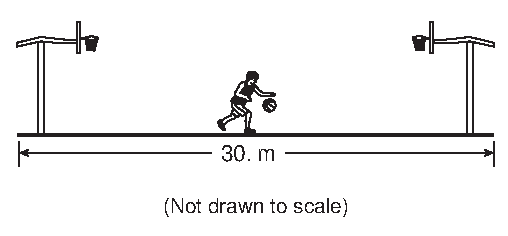
\includegraphics[keepaspectratio,scale=0.75]{June2012-Q01}
    \end{center}
    The magnitude of the player's total displacement after running the drill is:
    \begin{multicols}{2}
    \begin{choices}
      \correctchoice{\SI{0.0}{\meter}}
        \wrongchoice{\SI{30}{\meter}}
        \wrongchoice{\SI{60}{\meter}}
        \wrongchoice{\SI{180}{\meter}}
    \end{choices}
    \end{multicols}
\end{question}
}

\element{nysed}{
\begin{question}{June2012-Q02}
    In a drill during basketball practice,
        a player runs the length of the \SI{30}{\meter} court and back.
    The player does this three times in \SI{60}{\second}.
    \begin{center}
        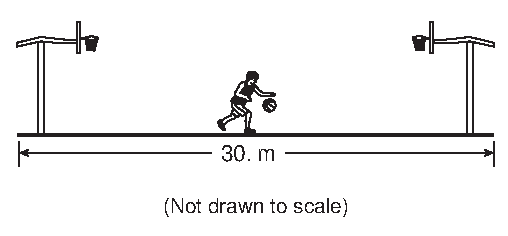
\includegraphics[keepaspectratio,scale=0.75]{June2012-Q01}
    \end{center}
    The average speed of the player during the drill is:
    \begin{multicols}{2}
    \begin{choices}
        \wrongchoice{\SI{0.0}{\meter\per\second}}
        \wrongchoice{\SI{0.50}{\meter\per\second}}
      \correctchoice{\SI{3.0}{\meter\per\second}}
        \wrongchoice{\SI{30}{\meter\per\second}}
    \end{choices}
    \end{multicols}
\end{question}
}


%% Section June2011
%%--------------------


%% Section June2010
%%--------------------
\element{nysed}{
\begin{question}{June2010-Q01}
    A baseball player runs \SI{27.4}{\meter} from the batter's box to first base,
        overruns first base by \SI{3.0}{\meter},
        and then returns to first base.
    Compared to the total distance traveled by the player,
        the magnitude of the player's total displacement from the batter's box is?
    \begin{multicols}{2}
    \begin{choices}
        \wrongchoice{\SI{3.0}{\meter} shorter}
      \correctchoice{\SI{6.0}{\meter} shorter}
        \wrongchoice{\SI{3.0}{\meter} longer}
        \wrongchoice{\SI{6.0}{\meter} longer}
    \end{choices}
    \end{multicols}
\end{question}
}


%% Section June2009
%%--------------------
\element{nysed}{
\begin{question}{June2009-Q01}
    On a highway, a car is driven \SI{80}{\kilo\meter} during the first \SI{1.00}{\hour} of travel,
        \SI{50}{\kilo\meter} during the next \SI{0.50}{\hour},
        and \SI{40}{\kilo\meter} in the final \SI{0.50}{\hour}.
    What is the car's average speed for the entire trip?
    \begin{multicols}{2}
    \begin{choices}
        \wrongchoice{\SI{45}{\kilo\meter\per\hour}}
        \wrongchoice{\SI{60}{\kilo\meter\per\hour}}
      \correctchoice{\SI{85}{\kilo\meter\per\hour}}
        \wrongchoice{\SI{170}{\kilo\meter\per\hour}}
    \end{choices}
    \end{multicols}
\end{question}
}

\element{nysed}{
\begin{question}{June2009-Q04}
    A high-speed train in Japan travels a distance of \SI{300}{\kilo\meter} in \SI{3.60e3}{\second}.
    What is the average speed of this train?
    \begin{multicols}{2}
    \begin{choices}
        \wrongchoice{\SI{1.20e-2}{\meter\per\second}}
        \wrongchoice{\SI{8.33e-2}{\meter\per\second}}
        \wrongchoice{\SI{12.0}{\meter\per\second}}
      \correctchoice{\SI{83.3}{\meter\per\second}}
    \end{choices}
    \end{multicols}
\end{question}
}


%% Section Jan2009
%%--------------------


%% Section June2008
%%--------------------
\element{nysed}{
\begin{question}{June2008-Q04}
    Approximately how much time does it take light to travel from Sun to Earth?
    \begin{multicols}{2}
    \begin{choices}
        \wrongchoice{\SI{2.00e-3}{\second}}
        \wrongchoice{\SI[retain-zero-exponent]{1.28e0}{\second}}
      \correctchoice{\SI{5.00e2}{\second}}
        \wrongchoice{\SI{4.50e19}{\second}}
    \end{choices}
    \end{multicols}
\end{question}
}


%% Section Jan2008
%%--------------------


%% Section June2007
%%--------------------


%% Section Jan2007
%%--------------------


%% Section June2006
%%--------------------


%% Section Jan2006
%%--------------------


%% Section June2005
%%--------------------


%% Section Jan2005
%%--------------------
\element{nysed}{
\begin{question}{Jan2005-Q02}
    In a \SI{4.0}{\kilo\meter} race, a runner completes the first kilometer in \SI{5.9}{\minute},
        the second kilometer in \SI{6.2}{\minute}, and the third kilometer in \SI{6.3}{\minute},
        and the final kilometer in \SI{6.0}{\minute}.
    The average speed of the runner for the race is approximately:
    \begin{multicols}{2}
    \begin{choices}
      \correctchoice{\SI{0.16}{\kilo\meter\per\minute}}
        \wrongchoice{\SI{0.33}{\kilo\meter\per\minute}}
        \wrongchoice{\SI{12}{\kilo\meter\per\minute}}
        \wrongchoice{\SI{24}{\kilo\meter\per\minute}}
    \end{choices}
    \end{multicols}
\end{question}
}


%% Section June2004
%%--------------------


%% Section Jan2004
%%--------------------


%% Section June2003
%%--------------------


%% Section Jan2003
%%--------------------


%% Section Aug2002
%%--------------------


%% Section June2002
%%--------------------


%% Section Jan2002
%%--------------------
\element{nysed}{
\begin{question}{Jan2002-Q03}
    A group of bike riders took a \SI{4.0}{\hour} trip.
    During the first \SI{3.0}{\hour},
        they traveled a total of \SI{50}{\kilo\meter},
        but during the last hour they traveled only \SI{10}{\kilo\meter}.
    What was the group's average speed for the entire trip?
    \begin{multicols}{2}
    \begin{choices}
      \correctchoice{\SI{15}{\kilo\meter\per\hour}}
        \wrongchoice{\SI{30}{\kilo\meter\per\hour}}
        \wrongchoice{\SI{40}{\kilo\meter\per\hour}}
        \wrongchoice{\SI{60}{\kilo\meter\per\hour}}
    \end{choices}
    \end{multicols}
\end{question}
}


%% Section June2001
%%--------------------
\element{nysed}{
\begin{question}{June2001-Q09}
    Two cars, $A$ and $B$, are \SI{400}{\meter} apart.
    Car $A$ travels due east at \SI{30}{\meter\per\second} on a collision course with car $B$,
        which travels due west at \SI{20}{\meter\per\second}.
    How much time elapses before the two cars collide?
    \begin{multicols}{2}
    \begin{choices}
      \correctchoice{\SI{8.0}{\second}}
        \wrongchoice{\SI{20}{\second}}
        \wrongchoice{\SI{13}{\second}}
        \wrongchoice{\SI{40}{\second}}
    \end{choices}
    \end{multicols}
\end{question}
}

\element{nysed}{
\begin{question}{June2001-Q53}
    A softball player leaves the batter's box,
        overruns first base by \SI{3.0}{\meter},
        and then returns to first base.
    Compared to the total distance traveled by the player,
        the magnitude of the player's total displacement from the batter's box is:
    \begin{multicols}{3}
    \begin{choices}
      \correctchoice{smaller}
        \wrongchoice{larger}
        \wrongchoice{the same}
    \end{choices}
    \end{multicols}
\end{question}
}


%% Section Jan2001
%%--------------------


%% Section June2000
%%--------------------


%% Section June1999
%%--------------------


%% Section June1998
%%--------------------
\element{nysed}{
\begin{question}{June1998-Q05}
    What is the average velocity of a car that travels \SI{30}{\kilo\meter} due west in \SI{0.50}{\hour}?
    \begin{multicols}{2}
    \begin{choices}
        \wrongchoice{\SI{15}{\kilo\meter\per\hour}}
        \wrongchoice{\SI{60}{\kilo\meter\per\hour}}
        \wrongchoice{\SI{15}{\kilo\meter\per\hour} west}
      \correctchoice{\SI{60}{\kilo\meter\per\hour} west}
    \end{choices}
    \end{multicols}
\end{question}
}


%% Section June1997
%%--------------------
\element{nysed}{
\begin{question}{June1997-Q02}
    A baseball pitcher throws a fastball at \SI{42}{\meter\per\second}.
    If the batter is \SI{18}{\meter} from the pitcher,
        approximately how much time does it take for the ball to reach the batter?
    \begin{multicols}{2}
    \begin{choices}
        \wrongchoice{\SI{1.0}{\second}}
        \wrongchoice{\SI{2.3}{\second}}
        \wrongchoice{\SI{0.86}{\second}}
      \correctchoice{\SI{0.43}{\second}}
    \end{choices}
    \end{multicols}
\end{question}
}


%% Section June1996
%%--------------------
\element{nysed}{
\begin{question}{June1996-Q01}
    A car travels between the \SI{100}{\meter} and \SI{250}{\meter} highway markers in \SI{10}{\second}.
    The average speed of the car during this interval is:
    \begin{multicols}{2}
    \begin{choices}
        \wrongchoice{\SI{10}{\meter\per\second}}
      \correctchoice{\SI{15}{\meter\per\second}}
        \wrongchoice{\SI{25}{\meter\per\second}}
        \wrongchoice{\SI{35}{\meter\per\second}}
    \end{choices}
    \end{multicols}
\end{question}
}


%% Section June1994
%%--------------------
\element{nysed}{
\begin{question}{June1994-Q44}
    The distance from the Moon to Earth is \SI{3.9e8}{\meter}.
    What is the time required for a light ray to travel from the Moon to Earth?
    \begin{multicols}{2}
    \begin{choices}
        \wrongchoice{\SI{0.65}{\second}}
      \correctchoice{\SI{1.3}{\second}}
        \wrongchoice{\SI{2.6}{\second}}
        \wrongchoice{\SI{3.9}{\second}}
    \end{choices}
    \end{multicols}
\end{question}
}


%% Section June1986
%%--------------------
\element{nysed}{
\begin{question}{June1986-Q02}
    The average speed of a plane was \SI{600}{\kilo\meter\per\hour}.
    How long did it take the plane to travel \SI{120}{\kilo\meter}?
    \begin{multicols}{2}
    \begin{choices}
      \correctchoice{\SI{0.2}{\hour}}
        \wrongchoice{\SI{0.5}{\hour}}
        \wrongchoice{\SI{0.7}{\hour}}
        \wrongchoice{\SI{5}{\hour}}
    \end{choices}
    \end{multicols}
\end{question}
}

\element{nysed}{
\begin{question}{June1986-Q19}
    It takes \SI{1}{\second} for a sound wave to travel from a source to observer $A$.
    How long does it take the same sound wave to travel in the same medium to observer $B$,
        who is located twice as far from the source as observer $A$?
    \begin{multicols}{4}
    \begin{choices}
        \wrongchoice{\SI{1/4}{\second}}
      \correctchoice{\SI{2}{\second}}
        \wrongchoice{\SI{1/2}{\second}}
        \wrongchoice{\SI{4}{\second}}
    \end{choices}
    \end{multicols}
\end{question}
}


%% Section June1985
%%--------------------
\element{nysed}{
\begin{question}{June1985-Q02}
    The distance-time graph below represents the position of an object moving in a straight line.
    \begin{center}
    \begin{tikzpicture}
        \begin{axis}[
            axis y line=left,
            axis x line=bottom,
            axis line style={->},
            xlabel={time},
            x unit=\si{\second},
            xtick={0,1,2,3,4,5,6},
            minor x tick num=1,
            ylabel={distance},
            y unit=\si{\meter},
            ytick={0,10,20,30},
            minor y tick num=1,
            xmin=0,xmax=6.3,
            ymin=0,ymax=31.5,
            width=0.8\columnwidth,
            height=0.5\columnwidth,
            grid=major,
            very thin,
        ]
        \addplot[line width=1pt,mark=\empty] plot coordinates { (0,0) (2,10) (4,30) (6,30)};
        \end{axis}
    \end{tikzpicture}
    \end{center}
    What is the speed of the object during the time interval $t=\SI{2.0}{\second}$ to $t=\SI{4.0}{\second}$?
    \begin{multicols}{2}
    \begin{choices}
        \wrongchoice{\SI{0.0}{\meter\per\second}}
        \wrongchoice{\SI{5.0}{\meter\per\second}}
        \wrongchoice{\SI{7.5}{\meter\per\second}}
      \correctchoice{\SI{10.}{\meter\per\second}}
    \end{choices}
    \end{multicols}
\end{question}
}



\endinput



%
%% Constant Accleration Questions
%% NYSED Physics Regents Examination
%%--------------------------------------------------

%% this section contains 59 problems


%% Section June2015
%%--------------------
\element{nysed}{
\begin{question}{June2015-Q40}
    A car, initially traveling at \SI{15}{\meter\per\second} north,
        accelerates to \SI{25}{\meter\per\second} north in \SI{4.0}{\second}.
    The magnitude of the average acceleration is:
    \begin{multicols}{2}
    \begin{choices}
      \correctchoice{\SI{2.5}{\meter\per\second\squared}}
        \wrongchoice{\SI{6.3}{\meter\per\second\squared}}
        \wrongchoice{\SI{10.}{\meter\per\second\squared}}
        \wrongchoice{\SI{20.}{\meter\per\second\squared}}
    \end{choices}
    \end{multicols}
\end{question}
}


%% Section June2014
%%--------------------
\element{nysed}{
\begin{question}{June2014-Q02}
    What is the final speed of an object that starts from rest and accelerates uniformly at \SI{4.0}{\meter\per\second\squared} over a distance of \SI{8.0}{\meter}?
    \begin{multicols}{2}
    \begin{choices}
      \correctchoice{\SI{8.0}{\meter\per\second}}
        \wrongchoice{\SI{16}{\meter\per\second}}
        \wrongchoice{\SI{32}{\meter\per\second}}
        \wrongchoice{\SI{64}{\meter\per\second}}
    \end{choices}
    \end{multicols}
\end{question}
}

\element{nysed}{
\begin{question}{June2014-Q07}
    A truck, initially traveling at a speed of \SI{22}{\meter\per\second},
        increases speed at a constant rate of \SI{2.4}{\meter\per\second\squared} for \SI{3.2}{\second}.
    What is the total distance traveled by the truck during this \SI{3.2}{\second} time interval?
    \begin{multicols}{2}
    \begin{choices}
      \correctchoice{\SI{83}{\meter}}
        \wrongchoice{\SI{70.}{\meter}}
        \wrongchoice{\SI{12}{\meter}}
        \wrongchoice{\SI{58}{\meter}}
    \end{choices}
    \end{multicols}
\end{question}
}


%% Section June2013
%%--------------------
\element{nysed}{
\begin{question}{June2013-Q03}
    A car traveling west in a straight line on a highway decreases its speed from \SI{30.0}{\meter\per\second} to \SI{23.0}{\meter\per\second} in \SI{2.00}{\second}.
    The car's average acceleration during this time interval is:
    \begin{multicols}{2}
    \begin{choices}
      \correctchoice{\SI{3.5}{\meter\per\second\squared} east}
        \wrongchoice{\SI{3.5}{\meter\per\second\squared} west}
        \wrongchoice{\SI{13}{\meter\per\second\squared} east}
        \wrongchoice{\SI{13}{\meter\per\second\squared} west}
    \end{choices}
    \end{multicols}
\end{question}
}

\element{nysed}{
\begin{question}{June2013-Q04}
    In a race, a runner traveled \SI{12}{\meter} in \SI{4.0}{\second} as she accelerated uniformly from rest.
    The magnitude of the acceleration of the runner was:
    \begin{multicols}{2}
    \begin{choices}
        \wrongchoice{\SI{0.25}{\meter\per\second\squared}}
      \correctchoice{\SI{1.5}{\meter\per\second\squared}}
        \wrongchoice{\SI{3.0}{\meter\per\second\squared}}
        \wrongchoice{\SI{48}{\meter\per\second\squared}}
    \end{choices}
    \end{multicols}
\end{question}
}


%% Section June2012
%%--------------------
\element{nysed}{
\begin{question}{June2012-Q06}
    A car, initially traveling east with a speed of \SI{5.0}{\meter\per\second},
        is accelerated uniformly at \SI{2.0}{\meter\per\second\squared} east for \SI{10}{\second} along a straight line.
    During this \SI{10}{\second} interval the car travels a total distance of:
    \begin{multicols}{2}
    \begin{choices}
        \wrongchoice{\SI{50}{\meter}}
        \wrongchoice{\SI{60}{\meter}}
        \wrongchoice{\SI{1.0e2}{\meter}}
      \correctchoice{\SI{1.5e2}{\meter}}
    \end{choices}
    \end{multicols}
\end{question}
}

\element{nysed}{
\begin{question}{June2012-Q08}
    A child riding a bicycle at \SI{15}{\meter\per\second} accelerates at \SI{-3.0}{\meter\per\second\squared} for \SI{4.0}{\second}.
    What is the child's speed at the end of this \SI{4.0}{\second} interval?
    \begin{multicols}{2}
    \begin{choices}
        \wrongchoice{\SI{12}{\meter\per\second}}
        \wrongchoice{\SI{27}{\meter\per\second}}
      \correctchoice{\SI{3.0}{\meter\per\second}}
        \wrongchoice{\SI{7.0}{\meter\per\second}}
    \end{choices}
    \end{multicols}
\end{question}
}


%% Section June2011
%%--------------------
\element{nysed}{
\begin{question}{June2011-Q02}
    If a car accelerates uniformly from rest to \SI{15}{\meter\per\second} over a distance of \SI{100}{\meter},
        the magnitude of a car's acceleration is:
    \begin{multicols}{2}
    \begin{choices}
        \wrongchoice{\SI{0.15}{\meter\per\second\squared}}
      \correctchoice{\SI{1.1}{\meter\per\second\squared}}
        \wrongchoice{\SI{2.3}{\meter\per\second\squared}}
        \wrongchoice{\SI{6.7}{\meter\per\second\squared}}
    \end{choices}
    \end{multicols}
\end{question}
}

\element{nysed}{
\begin{question}{June2011-Q03}
    An object accelerates uniformly from \SI{3.0}{\meter\per\second} east to \SI{8.0}{\meter\per\second} east in \SI{2.0}{\second}.
    What is the magnitude of the acceleration of the object?
    \begin{multicols}{2}
    \begin{choices}
      \correctchoice{\SI{2.5}{\meter\per\second\squared}}
        \wrongchoice{\SI{5.0}{\meter\per\second\squared}}
        \wrongchoice{\SI{5.5}{\meter\per\second\squared}}
        \wrongchoice{\SI{11}{\meter\per\second\squared}}
    \end{choices}
    \end{multicols}
\end{question}
}

\element{nysed}{
\begin{question}{June2011-Q04}
    A rock is dropped from a bridge.
    What happens to the magnitude of the acceleration and the speed of the rock as it falls?
    [Neglect friction.]
    \begin{choices}
        \wrongchoice{Both acceleration and speed increase.}
        \wrongchoice{Both acceleration and speed remain the same.}
        \wrongchoice{Acceleration increases and speed decreases.}
      \correctchoice{Acceleration remains the same and speed increases.}
    \end{choices}
\end{question}
}

\element{nysed}{
\begin{question}{June2011-Q05}
    A soccer ball is kicked on a level field has an initial vertical velocity component of \SI{15.0}{\meter\per\second}.
    Assuming the ball lands at the same height from which it was kicked,
        what is the total time the ball is in the air?
    [Neglect friction.]
    \begin{multicols}{2}
    \begin{choices}
        \wrongchoice{\SI{0.654}{\second}}
        \wrongchoice{\SI{1.53}{\second}}
      \correctchoice{\SI{3.06}{\second}}
        \wrongchoice{\SI{6.12}{\second}}
    \end{choices}
    \end{multicols}
\end{question}
}

\element{nysed}{
\begin{question}{June2011-Q37}
    The graph below shows the relationship between the speed and elapsed time for an object falling freely from rest near the surface of a planet.
    \begin{center}
    \begin{tikzpicture}
        \begin{axis}[
            axis y line=left,
            axis x line=bottom,
            axis line style={->},
            xlabel={Time},
            x unit=\si{\second},
            xtick={0.0,1.0,2.0,3.0,4.0},
            ylabel={Speed},
            y unit=\si{\meter\per\second},
            ytick={0.0,2.0,4.0,6.0,8.0,10.0},
            xmin=0,xmax=4,
            ymin=0,ymax=10,
            grid=major,
            width=0.8\columnwidth,
            height=0.5\columnwidth,
            very thin,
        ]
        \addplot[line width=1pt,domain=0:4]{8*x/3};
        \end{axis}
    \end{tikzpicture}
    \end{center}
    What is the total distance the object falls during
        the first \SI{3.0}{\second}?
    \begin{multicols}{2}
    \begin{choices}
      \correctchoice{\SI{12}{\meter}}
        \wrongchoice{\SI{24}{\meter}}
        \wrongchoice{\SI{44}{\meter}}
        \wrongchoice{\SI{72}{\meter}}
    \end{choices}
    \end{multicols}
\end{question}
}


%% Section June2010
%%--------------------
\element{nysed}{
\begin{question}{June2010-Q03}
    A car traveling on a straight road at \SI{15.0}{\meter\per\second} accelerates uniformly to a speed of \SI{21.0}{\meter\per\second} in \SI{12.0}{\second}.
    The total distance traveled by the car in this \SI{12.0}{\second} time interval is:
    \begin{multicols}{2}
    \begin{choices}
        \wrongchoice{\SI{36.0}{\meter}}
        \wrongchoice{\SI{180}{\meter}}
      \correctchoice{\SI{216}{\meter}}
        \wrongchoice{\SI{252}{\meter}}
    \end{choices}
    \end{multicols}
\end{question}
}


%% Section June2009
%%--------------------
\newcommand{\myJuneZeroNineQthirtySevenTikz}{
    \begin{tikzpicture}
        \begin{axis}[
            axis y line=left,
            axis x line=bottom,
            axis line style={->},
            xlabel={time},
            x unit=\si{\second},
            xtick={0,2,4,6},
            ylabel={velocity},
            y unit=\si{\meter\per\second},
            ytick={0,5,10,15},
            xmin=0,xmax=6.5,
            ymin=0,ymax=16,
            grid=major,
            width=0.8\columnwidth,
            height=0.5\columnwidth,
            very thin,
        ]
        \addplot[line width=1pt,domain=0:4]{2.5*x};
        \addplot[line width=1pt,domain=4:6]{10};
        \end{axis}
    \end{tikzpicture}
}

\element{nysed}{
\begin{question}{June2009-Q37}
    The diagram below represents the motion of a car during a \SI{6.0}{\second} time interval.
    \begin{center}
        \myJuneZeroNineQthirtySevenTikz
    \end{center}
    What is the acceleration of the car at $t=\SI{5.0}{\second}$?
    \begin{multicols}{2}
    \begin{choices}
      \correctchoice{\SI{0.0}{\meter\per\second\squared}}
        \wrongchoice{\SI{2.0}{\meter\per\second\squared}}
        \wrongchoice{\SI{2.5}{\meter\per\second\squared}}
        \wrongchoice{\SI{10.0}{\meter\per\second\squared}}
    \end{choices}
    \end{multicols}
\end{question}
}

\element{nysed}{
\begin{question}{June2009-Q38}
    The diagram below represents the motion of a car during a \SI{6.0}{\second} time interval.
    \begin{center}
        \myJuneZeroNineQthirtySevenTikz
    \end{center}
    What is the total distance traveled by the car during this \SI{6.0}{\second} interval?
    \begin{multicols}{2}
    \begin{choices}
        \wrongchoice{\SI{10.}{\meter}}
        \wrongchoice{\SI{20.}{\meter}}
      \correctchoice{\SI{40.}{\meter}}
        \wrongchoice{\SI{60.}{\meter}}
    \end{choices}
    \end{multicols}
\end{question}
}


%% Section Jan2009
%%--------------------
\element{nysed}{
\begin{question}{Jan2009-Q04}
    As a car driven south in a straight line with \emph{decreasing} speed,
        the acceleration of the car must be:
    \begin{choices}
      \correctchoice{directed northward}
        \wrongchoice{directed southward}
        \wrongchoice{zero}
        \wrongchoice{constant, but not zero}
    \end{choices}
\end{question}
}


%% Section June2008
%%--------------------
\element{nysed}{
\begin{question}{June2008-Q07}
    The speed of an object undergoing constant acceleration increases from \SI{8.0}{\meter\per\second} to \SI{16.0}{\meter\per\second} in \SI{10}{\second}.
    How far does the object travel during the \SI{10}{\second}?
    \begin{multicols}{2}
    \begin{choices}
        \wrongchoice{\SI{3.6e2}{\meter}}
        \wrongchoice{\SI{1.6e2}{\meter}}
      \correctchoice{\SI{1.2e2}{\meter}}
        \wrongchoice{\SI{8.0e1}{\meter}}
    \end{choices}
    \end{multicols}
\end{question}
}

\element{nysed}{
\begin{question}{June2008-Q37}
    The graph below represents the displacement of an object moving in a straight line as a function of time.
    \begin{center}
    \begin{tikzpicture}
        \begin{axis}[
            axis y line=left,
            axis x line=bottom,
            axis line style={->},
            xlabel={Time},
            x unit=\si{\second},
            xtick={0.0,2.0,4.0,6.0,8.0,10,0},
            ylabel={displacement},
            y unit=\si{\meter},
            ytick={0,4,8,12,16},
            xmin=0,xmax=10,
            ymin=0,ymax=16,
            grid=major,
            width=0.8\columnwidth,
            height=0.5\columnwidth,
            very thin,
        ]
        \addplot[line width=1pt,domain=0:4]{2*x};
        \addplot[line width=1pt,domain=4:6]{8};
        \addplot[line width=1pt,domain=6:10]{ 8 - 2*( (x-6) * (x-10) )};
        \end{axis}
    \end{tikzpicture}
    \end{center}
    What was the total distance traveled by the object during the \SI{10}{\second} time interval?
    \begin{multicols}{2}
    \begin{choices}
        \wrongchoice{\SI{0}{\meter}}
        \wrongchoice{\SI{8}{\meter}}
        \wrongchoice{\SI{16}{\meter}}
      \correctchoice{\SI{24}{\meter}}
    \end{choices}
    \end{multicols}
\end{question}
}


%% Section Jan2008
%%--------------------
\element{nysed}{
\begin{question}{Jan2008-Q02}
    A race car starting from rest accelerates uniformly at a rate of \SI{4.9}{\meter\per\second\squared}.
    What is the car's speed after it has traveled \SI{200}{\meter}.
    \begin{multicols}{2}
    \begin{choices}
      \correctchoice{\SI{44.3}{\meter\per\second}}
        \wrongchoice{\SI{62.6}{\meter\per\second}}
        \wrongchoice{\SI{1960}{\meter\per\second}}
        \wrongchoice{\SI{31.3}{\meter\per\second}}
    \end{choices}
    \end{multicols}
\end{question}
}


%% Section June2007
%%--------------------
\element{nysed}{
\begin{question}{June2007-Q02}
    An astronaut standing on a platform on the Moon drops a hammer.
    If the hammer falls \SI{6.0}{\meter} vertically in \SI{2.7}{\second},
        what is the acceleration?
    \begin{multicols}{2}
    \begin{choices}
      \correctchoice{\SI{1.6}{\meter\per\second\squared}}
        \wrongchoice{\SI{2.2}{\meter\per\second\squared}}
        \wrongchoice{\SI{4.4}{\meter\per\second\squared}}
        \wrongchoice{\SI{9.8}{\meter\per\second\squared}}
    \end{choices}
    \end{multicols}
\end{question}
}

\element{nysed}{
\begin{question}{June2007-Q40}
    An observer recorded the following data for the motion of a car undergoing constant acceleration.
    \begin{center}
    \begin{tabu}{cc}
        Time (\si{\second}) & Speed (\si{\meter\per\second}) \\
        \midrule
        3.0 & 4.0 \\
        5.0 & 7.0 \\
        6.0 & 8.5 \\
    \end{tabu}
    \end{center}
    What was the magnitude of the acceleration of the car?
    \begin{multicols}{2}
    \begin{choices}
        \wrongchoice{\SI{1.3}{\meter\per\second\squared}}
        \wrongchoice{\SI{2.0}{\meter\per\second\squared}}
      \correctchoice{\SI{1.5}{\meter\per\second\squared}}
        \wrongchoice{\SI{4.5}{\meter\per\second\squared}}
    \end{choices}
    \end{multicols}
\end{question}
}


%% Section Jan2007
%%--------------------
\element{nysed}{
\begin{question}{Jan2007-Q03}
    A car increases its speed from \SI{9.6}{\meter\per\second} to \SI{11.2}{\meter\per\second} in \SI{4.0}{\second}.
    The average acceleration of the car during this \SI{4.0}{\second} interval is:
    \begin{multicols}{2}
    \begin{choices}
      \correctchoice{\SI{0.40}{\meter\per\second\squared}}
        \wrongchoice{\SI{2.4}{\meter\per\second\squared}}
        \wrongchoice{\SI{2.8}{\meter\per\second\squared}}
        \wrongchoice{\SI{5.2}{\meter\per\second\squared}}
    \end{choices}
    \end{multicols}
\end{question}
}

\element{nysed}{
\begin{question}{Jan2007-Q36}
    A cart travels with a constant nonzero acceleration along a straight line.
    Which graph best represents the relationship between the distance the cart travels and the time of travel?
    \begin{multicols}{2}
    \begin{choices}
        \AMCboxDimensions{down=-2.5em}
        \correctchoice{
            \begin{tikzpicture}
                \begin{axis}[
                    axis y line=left,
                    axis x line=bottom,
                    axis line style={->},
                    xlabel={time},
                    xtick=\empty,
                    ylabel={distance},
                    ytick=\empty,
                    xmin=0,xmax=11,
                    ymin=0,ymax=11,
                    width=\columnwidth,
                    very thin,
                ]
                \addplot[line width=1pt,domain=0:10]{0.1 * x*x};
                \end{axis}
            \end{tikzpicture}
        }
        \wrongchoice{
            \begin{tikzpicture}
                \begin{axis}[
                    axis y line=left,
                    axis x line=bottom,
                    axis line style={->},
                    xlabel={time},
                    xtick=\empty,
                    ylabel={distance},
                    ytick=\empty,
                    xmin=0,xmax=11,
                    ymin=0,ymax=11,
                    width=\columnwidth,
                    very thin,
                ]
                \addplot[line width=1pt,domain=0:10]{10-x};
                \end{axis}
            \end{tikzpicture}
        }
        \wrongchoice{
            \begin{tikzpicture}
                \begin{axis}[
                    axis y line=left,
                    axis x line=bottom,
                    axis line style={->},
                    xlabel={time},
                    xtick=\empty,
                    ylabel={distance},
                    ytick=\empty,
                    xmin=0,xmax=185,
                    ymin=0,ymax=10,
                    width=\columnwidth,
                    very thin,
                ]
                \addplot[line width=1pt,domain=0:180]{8*sin(x)};
                \end{axis}
            \end{tikzpicture}
        }
        \wrongchoice{
            \begin{tikzpicture}
                \begin{axis}[
                    axis y line=left,
                    axis x line=bottom,
                    axis line style={->},
                    xlabel={time},
                    xtick=\empty,
                    ylabel={distance},
                    ytick=\empty,
                    xmin=0,xmax=11,
                    ymin=0,ymax=11,
                    width=\columnwidth,
                    very thin,
                ]
                \addplot[line width=1pt,domain=0:10]{x};
                \end{axis}
            \end{tikzpicture}
        }
    \end{choices}
    \end{multicols}
\end{question}
}


%% Section June2006
%%--------------------
\element{nysed}{
\begin{question}{June2006-Q02}
    A rocket initially at rest on the ground lifts off vertically with a constant acceleration of \SI{2.0e1}{\meter\per\second\squared}.
    How long will it take the rocket to reach an altitude of \SI{9.0e3}{\meter}?
    \begin{multicols}{2}
    \begin{choices}
      \correctchoice{\SI{3.0e1}{\second}}
        \wrongchoice{\SI{4.3e1}{\second}}
        \wrongchoice{\SI{4.5e2}{\second}}
        \wrongchoice{\SI{9.0e2}{\second}}
    \end{choices}
    \end{multicols}
\end{question}
}


%% Section Jan2006
%%--------------------
\element{nysed}{
\begin{question}{Jan2006-Q01}
    The speed of a wagon increases from \SI{2.5}{\meter\per\second} to \SI{9.0}{\meter\per\second} in \SI{3.0}{\second} as it accelerates uniformly down a hill.
    what is the magnitude of the acceleration of the wagon during this \SI{3.0}{\second} interval?
    \begin{multicols}{2}
    \begin{choices}
        \wrongchoice{\SI{0.83}{\meter\per\second\squared}}
      \correctchoice{\SI{2.2}{\meter\per\second\squared}}
        \wrongchoice{\SI{3.0}{\meter\per\second\squared}}
        \wrongchoice{\SI{3.8}{\meter\per\second\squared}}
    \end{choices}
    \end{multicols}
\end{question}
}

\element{nysed}{
\begin{question}{Jan2006-Q38}
    The graph below represents the relationship between speed and time for an object moving along a straight line.
    \begin{center}
    \begin{tikzpicture}
        \begin{axis}[
            axis y line=left,
            axis x line=bottom,
            axis line style={->},
            title={Speed vs. Time},
            xlabel={time},
            xtick={0,1,2,3,4,5},
            x unit=\si{\second},
            ylabel={speed},
            y unit=\si{\meter\per\second},
            ytick={0,5,10,15,20,25},
            xmin=0,xmax=5,
            ymin=0,ymax=25,
            grid=major,
            width=0.8\columnwidth,
            height=0.5\columnwidth,
            very thin,
        ]
        \addplot[line width=1pt,domain=0:5]{5*x};
        \end{axis}
    \end{tikzpicture}
    \end{center}
    What is the total distance traveled by the object during the first \SI{4}{\second}?
    \begin{multicols}{2}
    \begin{choices}
        \wrongchoice{\SI{5}{\meter}}
        \wrongchoice{\SI{20}{\meter}}
      \correctchoice{\SI{40}{\meter}}
        \wrongchoice{\SI{80}{\meter}}
    \end{choices}
    \end{multicols}
\end{question}
}


%% Section Jan2005
%%--------------------
\element{nysed}{
\begin{question}{Jan2005-Q36}
    Which pair of graphs represents the same motion of an object?
    \begin{choices}
        \AMCboxDimensions{down=-2.5em}
        \correctchoice{
            \begin{tikzpicture}
                \begin{groupplot}[
                        axis y line=left,
                        axis x line=bottom,
                        axis line style={->},
                        group style={group size=2 by 1},
                        xtick=\empty,
                        ytick=\empty,
                        width=0.5\columnwidth,
                    ]
                    \nextgroupplot[
                        xlabel={time},
                        ylabel={displacement},
                        xmin=0,xmax=11,
                        ymin=0,ymax=11,
                    ] \addplot[line width=1pt,domain=0:10] {0.1*x*x};
                    \nextgroupplot[
                        xlabel={time},
                        ylabel={velocity},
                        xmin=0,xmax=11,
                        ymin=0,ymax=11,
                    ] \addplot[line width=1pt,domain=0:10] {x};
                \end{groupplot}
            \end{tikzpicture}
        }
        \wrongchoice{
            \begin{tikzpicture}
                \begin{groupplot}[
                        axis y line=left,
                        axis x line=middle,
                        axis line style={->},
                        group style={group size=2 by 1},
                        xtick=\empty,
                        ytick=\empty,
                        width=0.5\columnwidth,
                    ]
                    \nextgroupplot[
                        xlabel={time},
                        ylabel={displacement},
                        x label style={anchor=north east},
                        xmin=0,xmax=11,
                        ymin=-5.5,ymax=5.5,
                    ] \addplot[line width=1pt,domain=0:10] {-5+x};
                    \nextgroupplot[
                        xlabel={time},
                        ylabel={velocity},
                        xmin=0,xmax=11,
                        ymin=-5.5,ymax=5.5,
                    ] \addplot[line width=1pt,domain=0:10] {-3};
                \end{groupplot}
            \end{tikzpicture}
        }
        \wrongchoice{
            \begin{tikzpicture}
                \begin{groupplot}[
                        axis y line=left,
                        axis x line=middle,
                        axis line style={->},
                        group style={group size=2 by 1},
                        xtick=\empty,
                        ytick=\empty,
                        width=0.5\columnwidth,
                    ]
                    \nextgroupplot[
                        xlabel={time},
                        ylabel={displacement},
                        xmin=0,xmax=11,
                        ymin=-5.5,ymax=5.5,
                    ] \addplot[line width=1pt,domain=0:10] {5-x};
                    \nextgroupplot[
                        xlabel={time},
                        ylabel={velocity},
                        x label style={anchor=north east},
                        xmin=0,xmax=11,
                        ymin=-5.5,ymax=5.5,
                    ] \addplot[line width=1pt,domain=0:10] {-5+x};
                \end{groupplot}
            \end{tikzpicture}
        }
        \wrongchoice{
            \begin{tikzpicture}
                \begin{groupplot}[
                        axis y line=left,
                        axis x line=bottom,
                        axis line style={->},
                        group style={group size=2 by 1},
                        xtick=\empty,
                        ytick=\empty,
                        width=0.5\columnwidth,
                    ]
                    \nextgroupplot[
                        xlabel={time},
                        ylabel={displacement},
                        xmin=0,xmax=11,
                        ymin=0,ymax=11,
                    ] \addplot[line width=1pt,domain=0:10] {-0.4 *x * (x-10)};
                    \nextgroupplot[
                        xlabel={time},
                        ylabel={velocity},
                        xmin=0,xmax=11,
                        ymin=0,ymax=11,
                    ] \addplot[line width=1pt,domain=0:10] {8};
                \end{groupplot}
            \end{tikzpicture}
        }
    \end{choices}
\end{question}
}



%% Section Jan2004
%%--------------------
\element{nysed}{
\begin{question}{Jan2004-Q03}
    A skater increases her speed uniformly from \SI{2.0}{\meter\per\second}
        to \SI{7.0}{\meter\per\second} over a distance of \SI{12}{\meter}.
    The magnitude of her acceleration as she travels this \SI{12}{\meter} is:
    \begin{multicols}{2}
    \begin{choices}
      \correctchoice{\SI{1.9}{\meter\per\second\squared}}
        \wrongchoice{\SI{2.2}{\meter\per\second\squared}}
        \wrongchoice{\SI{2.4}{\meter\per\second\squared}}
        \wrongchoice{\SI{3.8}{\meter\per\second\squared}}
    \end{choices}
    \end{multicols}
\end{question}
}


%% Section June2003
%%--------------------
\element{nysed}{
\begin{question}{June2003-Q03}
    A car initially traveling at a speed of \SI{16}{\meter\per\second} accelerates uniformly to a speed of \SI{20}{\meter\per\second} over a distance of \SI{36}{\meter}.
    What is the magnitude of the car's acceleration?
    \begin{multicols}{2}
    \begin{choices}
      \correctchoice{\SI{2.0}{\meter\per\second\squared}}
        \wrongchoice{\SI{0.22}{\meter\per\second\squared}}
        \wrongchoice{\SI{9.0}{\meter\per\second\squared}}
        \wrongchoice{\SI{0.11}{\meter\per\second\squared}}
    \end{choices}
    \end{multicols}
\end{question}
}


%% Section Jan2003
%%--------------------

\element{nysed}{
\begin{question}{Jan2003-Q45}
    Which graph best represents the motion of a block accelerating uniformly down an inclined plane?
    \begin{multicols}{2}
    \begin{choices}
        \AMCboxDimensions{down=-2.5em}
        \correctchoice{
            \begin{tikzpicture}
                \begin{axis}[
                    axis y line=left,
                    axis x line=bottom,
                    axis line style={->},
                    xlabel={time},
                    xtick=\empty,
                    ylabel={distance},
                    ytick=\empty,
                    xmin=0,xmax=11,
                    ymin=0,ymax=11,
                    width=\columnwidth,
                    very thin,
                ]
                \addplot[line width=1pt,domain=0:10]{0.1*x*x};
                \end{axis}
            \end{tikzpicture}
        }
        \wrongchoice{
            \begin{tikzpicture}
                \begin{axis}[
                    axis y line=left,
                    axis x line=bottom,
                    axis line style={->},
                    xlabel={time},
                    xtick=\empty,
                    ylabel={distance},
                    ytick=\empty,
                    xmin=0,xmax=11,
                    ymin=0,ymax=11,
                    width=\columnwidth,
                    very thin,
                ]
                \addplot[line width=1pt,domain=0:10]{x};
                \end{axis}
            \end{tikzpicture}
        }
        \wrongchoice{
            \begin{tikzpicture}
                \begin{axis}[
                    axis y line=left,
                    axis x line=bottom,
                    axis line style={->},
                    xlabel={time},
                    xtick=\empty,
                    ylabel={distance},
                    ytick=\empty,
                    xmin=0,xmax=11,
                    ymin=0,ymax=11,
                    width=\columnwidth,
                    very thin,
                ]
                \addplot[line width=1pt,domain=0:10]{7};
                \end{axis}
            \end{tikzpicture}
        }
        \wrongchoice{
            \begin{tikzpicture}
                \begin{axis}[
                    axis y line=left,
                    axis x line=bottom,
                    axis line style={->},
                    xlabel={time},
                    xtick=\empty,
                    ylabel={distance},
                    ytick=\empty,
                    xmin=0,xmax=11,
                    ymin=0,ymax=11,
                    width=\columnwidth,
                    very thin,
                ]
                \addplot[line width=1pt,domain=0:5]{1+1.2*x};
                \addplot[line width=1pt,domain=5:10]{7};
                \end{axis}
            \end{tikzpicture}
        }
    \end{choices}
    \end{multicols}
\end{question}
}


%% Section Aug2002
%%--------------------
\element{nysed}{
\begin{question}{Aug2002-Q02}
    The speed of a car is increased uniformly from \SI{20}{\meter\per\second} to \SI{30}{\meter\per\second} in \SI{4.0}{\second}.
    The magnitude of the car's average acceleration in this \SI{4.0}{\second} interval is:
    \begin{multicols}{2}
    \begin{choices}
        \wrongchoice{\SI{0.40}{\meter\per\second\squared}}
      \correctchoice{\SI{2.5}{\meter\per\second\squared}}
        \wrongchoice{\SI{10}{\meter\per\second\squared}}
        \wrongchoice{\SI{13}{\meter\per\second\squared}}
    \end{choices}
    \end{multicols}
\end{question}
}

\element{nysed}{
\begin{question}{Aug2002-Q03}
    A roller coaster, traveling with an initial speed of \SI{15}{\meter\per\second},
        decelerates uniformly at \SI{-7.0}{\meter\per\second\squared} to a full stop.
    Approximately how far does the roller coaster travel during its deceleration?
    \begin{multicols}{2}
    \begin{choices}
        \wrongchoice{\SI{1.0}{\meter}}
        \wrongchoice{\SI{2.0}{\meter}}
      \correctchoice{\SI{16}{\meter}}
        \wrongchoice{\SI{32}{\meter}}
    \end{choices}
    \end{multicols}
\end{question}
}

\element{nysed}{
\begin{question}{Aug2002-Q39}
    The graph below shows the velocity of a race car moving along a straight line as a function of time.
    \begin{center}
    \begin{tikzpicture}
        \begin{axis}[
            clip=false,
            axis y line=left,
            axis x line=bottom,
            axis line style={->},
            xlabel={time},
            x unit=\si{\second},
            xtick={0,1,2,3,4},
            ylabel={velocity},
            y unit=\si{\meter\per\second},
            ytick={0,10,20,30,40},
            xmin=0,xmax=4.1,
            ymin=0,ymax=42,
            grid=major,
            width=0.8\columnwidth,
            height=0.5\columnwidth,
            very thin,
        ]
        \addplot[line width=1pt,domain=0:4]{10*x};
        \end{axis}
    \end{tikzpicture}
    \end{center}
    What is the magnitude of the displacement of the car from $t=\SI{2.0}{\second}$ to $t=\SI{4.0}{\second}$?
    \begin{multicols}{2}
    \begin{choices}
        \wrongchoice{\SI{20}{\meter}}
        \wrongchoice{\SI{40}{\meter}}
      \correctchoice{\SI{60}{\meter}}
        \wrongchoice{\SI{80}{\meter}}
    \end{choices}
    \end{multicols}
\end{question}
}


%% Section June2002
%%--------------------
\element{nysed}{
\begin{question}{June2002-Q03}
    An object with an initial speed of \SI{4.0}{\meter\per\second} accelerates uniformly at \SI{2.0}{\meter\per\second\squared} in the direction of its motion for a distance of \SI{5.0}{\meter}.
    What is the final speed of the object?
    \begin{multicols}{2}
    \begin{choices}
      \correctchoice{\SI{6.0}{\meter\per\second}}
        \wrongchoice{\SI{10}{\meter\per\second}}
        \wrongchoice{\SI{14}{\meter\per\second}}
        \wrongchoice{\SI{36}{\meter\per\second}}
    \end{choices}
    \end{multicols}
\end{question}
}

\element{nysed}{
\begin{question}{June2002-Q04}
    After a model rocket reached its maximum height, it then took \SI{5.0}{\second} to return to the launch site.
    What is the approximate maximum height reached by the rocket?
    [Neglect air resistance]
    \begin{multicols}{2}
    \begin{choices}
        \wrongchoice{\SI{49}{\meter}}
        \wrongchoice{\SI{98}{\meter}}
      \correctchoice{\SI{120}{\meter}}
        \wrongchoice{\SI{250}{\meter}}
    \end{choices}
    \end{multicols}
\end{question}
}

\element{nysed}{
\begin{question}{June2002-Q36}
    The displacement-time graph below represents the motion of a cart initially moving in a straight line.
    \begin{center}
    \begin{tikzpicture}
        \begin{axis}[
            clip=false,
            axis y line=left,
            axis x line=bottom,
            axis line style={->},
            xlabel={time},
            xtick=\empty,
            ylabel={displacement},
            ytick=\empty,
            xmin=0,xmax=26,
            ymin=0,ymax=12,
            width=0.8\columnwidth,
            height=0.5\columnwidth,
            very thin,
        ]
        \addplot[line width=1pt,domain=0:5]{0.24*x*x}
            node[black,pos=0,anchor=north] {$A$};
        \addplot[line width=1pt,domain=5:14]{6 + (x-5)/3}
            node[black,pos=0,anchor=south] {$B$};
        \addplot[line width=1pt,domain=14:20]{9}
            node[black,pos=0,anchor=south] {$C$};
        \addplot[line width=1pt,domain=20:24]{9 - 1.25*(x-20)}
            node[black,pos=0,anchor=south west] {$D$}
            node[black,pos=1,anchor=west] {$E$};
        \addplot[only marks,mark=*,mark size=2pt] coordinates
            { (0,0) (5,6) (14,9) (20,9) (24,4) };
        \end{axis}
    \end{tikzpicture}
    \end{center}
    During which interval is the cart moving forward at constant speed?
    \begin{multicols}{2}
    \begin{choices}
        \wrongchoice{$AB$}
      \correctchoice{$BC$}
        \wrongchoice{$CD$}
        \wrongchoice{$DE$}
    \end{choices}
    \end{multicols}
\end{question}
}


%% Section Jan2002
%%--------------------
\element{nysed}{
\begin{question}{Jan2002-Q04}
    A skier starting from rest skis straight down a slope \SI{50}{\meter} long in \SI{5.0}{\second}.
    What is the magnitude of the acceleration of the skier?
    \begin{multicols}{2}
    \begin{choices}
        \wrongchoice{\SI{20}{\meter\per\second\squared}}
        \wrongchoice{\SI{9.8}{\meter\per\second\squared}}
        \wrongchoice{\SI{5.0}{\meter\per\second\squared}}
      \correctchoice{\SI{4.0}{\meter\per\second\squared}}
    \end{choices}
    \end{multicols}
\end{question}
}


%% Section June2001
%%--------------------
\element{nysed}{
\begin{question}{June2001-Q03}
    Which graph best represents the motion of an object whose speed is increasing?
    \begin{multicols}{2}
    \begin{choices}
        \AMCboxDimensions{down=-2.5em}
        \correctchoice{
            \begin{tikzpicture}
                \begin{axis}[
                    axis y line=left,
                    axis x line=bottom,
                    axis line style={->},
                    xlabel={time},
                    xtick=\empty,
                    ylabel={distance},
                    ytick=\empty,
                    xmin=0,xmax=11,
                    ymin=0,ymax=11,
                    width=\columnwidth,
                    very thin,
                ]
                \addplot[line width=1pt,domain=0:10]{0.1*x*x};
                \end{axis}
            \end{tikzpicture}
        }
        \wrongchoice{
            \begin{tikzpicture}
                \begin{axis}[
                    axis y line=left,
                    axis x line=bottom,
                    axis line style={->},
                    xlabel={time},
                    xtick=\empty,
                    ylabel={distance},
                    ytick=\empty,
                    xmin=0,xmax=11,
                    ymin=0,ymax=11,
                    width=\columnwidth,
                    very thin,
                ]
                \addplot[line width=1pt,domain=0:10]{x};
                \end{axis}
            \end{tikzpicture}
        }
        \wrongchoice{
            \begin{tikzpicture}
                \begin{axis}[
                    axis y line=left,
                    axis x line=bottom,
                    axis line style={->},
                    xlabel={time},
                    xtick=\empty,
                    ylabel={distance},
                    ytick=\empty,
                    xmin=0,xmax=11,
                    ymin=0,ymax=11,
                    width=\columnwidth,
                    very thin,
                ]
                \addplot[line width=1pt,domain=0:10]{10-x};
                \end{axis}
            \end{tikzpicture}
        }
        \wrongchoice{
            \begin{tikzpicture}
                \begin{axis}[
                    axis y line=left,
                    axis x line=bottom,
                    axis line style={->},
                    xlabel={time},
                    xtick=\empty,
                    ylabel={distance},
                    ytick=\empty,
                    xmin=0,xmax=11,
                    ymin=0,ymax=11,
                    width=\columnwidth,
                    very thin,
                ]
                \addplot[line width=1pt,domain=0:10]{10/x};
                \end{axis}
            \end{tikzpicture}
        }
    \end{choices}
    \end{multicols}
\end{question}
}

\element{nysed}{
\begin{question}{June2001-Q05}
    A car having an initial velocity of \SI{12}{\meter\per\second} east slows uniformly to \SI{2}{\meter\per\second} east in \SI{4.0}{\second}.
    The acceleration of the car during this \SI{4.0}{\second} interval is:
    \begin{multicols}{2}
    \begin{choices}
      \correctchoice{\SI{2.5}{\meter\per\second\squared} west}
        \wrongchoice{\SI{2.5}{\meter\per\second\squared} east}
        \wrongchoice{\SI{6.0}{\meter\per\second\squared} west}
        \wrongchoice{\SI{6.0}{\meter\per\second\squared} east}
    \end{choices}
    \end{multicols}
\end{question}
}

\element{nysed}{
\begin{question}{June2001-Q14}
    An airplane originally at rest on a runway accelerates uniformly at \SI{6.0}{\meter\per\second\squared} for \SI{12}{\second}.
    During this \SI{12}{\second} interval,
        the airplane travels a distance of approximately:
    \begin{multicols}{2}
    \begin{choices}
        \wrongchoice{\SI{72}{\meter}}
        \wrongchoice{\SI{220}{\meter}}
      \correctchoice{\SI{430}{\meter}}
        \wrongchoice{\SI{860}{\meter}}
    \end{choices}
    \end{multicols}
\end{question}
}


%% Section Jan2001
%%--------------------
\element{nysed}{
\begin{question}{Jan2001-Q02}
    The diagram below represents the relationship between velocity and time for four cars,
        $A$, $B$, $C$, and $D$, in straight-line motion.
    \begin{center}
    \begin{tikzpicture}
        \begin{axis}[
            axis y line=left,
            axis x line=bottom,
            axis line style={->},
            xlabel={time},
            x unit=\si{\second},
            xtick={0,5,10,15,20},
            ylabel={velocity},
            ytick=\empty,
            xmin=0,xmax=21,
            ymin=0,ymax=10,
            width=0.98\columnwidth,
            height=0.618\columnwidth,
            very thin,
        ]
        \addplot[line width=0.7pt,domain=0:20]{8}
            node[pos=0.1,anchor=south east] {$A$};
        \addplot[line width=1pt,domain=0:20]{4 + 4*x/15}
            node[pos=0.1,anchor=south east] {$B$};
        \addplot[line width=1.25pt,domain=0:20]{8*x/15}
            node[pos=0.1,anchor=south east] {$C$};
        \addplot[line width=1.5pt,domain=10:20]{8*(x-10)/5}
            node[pos=0.0,anchor=south east] {$D$};
        \end{axis}
    \end{tikzpicture}
    \end{center}
    Which car has the greatest acceleration during the time interval \SI{10}{\second} to \SI{15}{\second}?
    \begin{multicols}{4}
    \begin{choices}[o]
        \wrongchoice{$A$}
        \wrongchoice{$B$}
        \wrongchoice{$C$}
      \correctchoice{$D$}
    \end{choices}
    \end{multicols}
\end{question}
}

\element{nysed}{
\begin{question}{Jan2001-Q14}
    %% NOTE: Reword
    %The graph below represents the displacment ($x$)
    %    of an object with respect to time ($t$).
    The graph below represents the motion of an object.
    \begin{center}
    \begin{tikzpicture}
        \begin{axis}[
            axis y line=left,
            axis x line=bottom,
            axis line style={->},
            xlabel={time},
            xtick=\empty,
            ylabel={displacement},
            ytick=\empty,
            xmin=0,xmax=10,
            ymin=0,ymax=10,
            width=0.8\columnwidth,
            height=0.5\columnwidth,
            very thin,
        ]
        \addplot[line width=1pt,domain=0:10]{x};
        \end{axis}
    \end{tikzpicture}
    \end{center}
    According the the graph, as time increases,
        the velocity of the object:
    \begin{choices}
        \wrongchoice{decreases}
        \wrongchoice{increases}
      \correctchoice{remains the same}
    \end{choices}
\end{question}
}


%% Section June2000
%%--------------------
\element{nysed}{
\begin{question}{June2000-Q02}
    Which pair of graphs represents the same motion?
    \begin{choices}
        \AMCboxDimensions{down=-2.5em}
        \correctchoice{
            \begin{tikzpicture}
                \begin{groupplot}[
                        axis y line=left,
                        axis x line=bottom,
                        axis line style={->},
                        group style={group size=2 by 1},
                        xtick=\empty,
                        ytick=\empty,
                        width=0.5\columnwidth,
                    ]
                    \nextgroupplot[
                        xlabel={time},
                        ylabel={displacement},
                        xmin=0,xmax=11,
                        ymin=0,ymax=11,
                    ] \addplot[line width=1pt,domain=0:10] {x};
                    \nextgroupplot[
                        xlabel={time},
                        ylabel={velocity},
                        xmin=0,xmax=11,
                        ymin=0,ymax=11,
                    ] \addplot[line width=1pt,domain=0:10] {5};
                \end{groupplot}
            \end{tikzpicture}
        }
        \wrongchoice{
            \begin{tikzpicture}
                \begin{groupplot}[
                        axis y line=left,
                        axis x line=bottom,
                        axis line style={->},
                        group style={group size=2 by 1},
                        xtick=\empty,
                        ytick=\empty,
                        width=0.5\columnwidth,
                    ]
                    \nextgroupplot[
                        xlabel={time},
                        ylabel={displacement},
                        xmin=0,xmax=11,
                        ymin=0,ymax=11,
                    ] \addplot[line width=1pt,domain=0:10] {5};
                    \nextgroupplot[
                        xlabel={time},
                        ylabel={velocity},
                        xmin=0,xmax=11,
                        ymin=0,ymax=11,
                    ] \addplot[line width=1pt,domain=0:10] {x};
                \end{groupplot}
            \end{tikzpicture}
        }
        \wrongchoice{
            \begin{tikzpicture}
                \begin{groupplot}[
                        axis y line=left,
                        axis x line=bottom,
                        axis line style={->},
                        group style={group size=2 by 1},
                        xtick=\empty,
                        ytick=\empty,
                        width=0.5\columnwidth,
                    ]
                    \nextgroupplot[
                        xlabel={time},
                        ylabel={displacement},
                        xmin=0,xmax=11,
                        ymin=0,ymax=11,
                    ] \addplot[line width=1pt,domain=0:10] {10-x};
                    \nextgroupplot[
                        xlabel={time},
                        ylabel={velocity},
                        xmin=0,xmax=11,
                        ymin=0,ymax=11,
                    ] \addplot[line width=1pt,domain=0:10] {x};
                \end{groupplot}
            \end{tikzpicture}
        }
        \wrongchoice{
            \begin{tikzpicture}
                \begin{groupplot}[
                        axis y line=left,
                        axis x line=bottom,
                        axis line style={->},
                        group style={group size=2 by 1},
                        xtick=\empty,
                        ytick=\empty,
                        width=0.5\columnwidth,
                    ]
                    \nextgroupplot[
                        xlabel={time},
                        ylabel={displacement},
                        xmin=0,xmax=11,
                        ymin=0,ymax=11,
                    ] \addplot[line width=1pt,domain=0:10] {x};
                    \nextgroupplot[
                        xlabel={time},
                        ylabel={velocity},
                        xmin=0,xmax=11,
                        ymin=0,ymax=11,
                    ] \addplot[line width=1pt,domain=0:10] {x};
                \end{groupplot}
            \end{tikzpicture}
        }
    \end{choices}
\end{question}
}

\element{nysed}{
\begin{question}{June2000-Q03}
    A runner starts from rest and accelerates uniformly to a speed of \SI{8.0}{\meter\per\second} in \SI{4.0}{\second}.
    The magnitude of the acceleration of the runner is:
    \begin{multicols}{2}
    \begin{choices}
        \wrongchoice{\SI{0.50}{\meter\per\second\squared}}
      \correctchoice{\SI{2.0}{\meter\per\second\squared}}
        \wrongchoice{\SI{9.8}{\meter\per\second\squared}}
        \wrongchoice{\SI{32}{\meter\per\second\squared}}
    \end{choices}
    \end{multicols}
\end{question}
}


%% Section June1999
%%--------------------
\element{nysed}{
\begin{question}{June1999-Q02}
    A truck with an initial speed of \SI{12}{\meter\per\second} accelerates uniformly at \SI{2.0}{\meter\per\second\squared} for \SI{3.0}{\second}.
    What is the total distance traveled by the truck during this \SI{3.0}{\second} interval?
    \begin{multicols}{2}
    \begin{choices}
        \wrongchoice{\SI{9.0}{\meter}}
        \wrongchoice{\SI{25}{\meter}}
        \wrongchoice{\SI{36}{\meter}}
      \correctchoice{\SI{45}{\meter}}
    \end{choices}
    \end{multicols}
\end{question}
}

\element{nysed}{
\begin{question}{June1999-Q05}
    The graph below represents the relationship between the displacement of an object and its time of travel along a straight line.
    \begin{center}
    \begin{tikzpicture}
        \begin{axis}[
            axis line style={->},
            axis y line=left,
            axis x line=bottom,
            label={displacement vs. time},
            xlabel={time},
            x unit=\si{\second},
            xtick={0,1,2,3,4,5,6,7,8},
            ylabel={displacement},
            y unit=\si{\meter},
            ytick={0,2,4,6,8,10},
            xmin=0,xmax=8.1,
            ymin=0,ymax=10.1,
            grid=major,
            width=0.8\columnwidth,
            height=0.5\columnwidth,
            very thin,
        ]
        \addplot[line width=1pt,domain=0:2]{4*x};
        \addplot[line width=1pt,domain=2:4]{8};
        \addplot[line width=1pt,domain=4:8]{16-2*x};
        \end{axis}
    \end{tikzpicture}
    \end{center}
    What is the magnitude of the object's total displacement after \SI{8.0}{\second}?
    \begin{multicols}{2}
    \begin{choices}
      \correctchoice{\SI{0}{\meter}}
        \wrongchoice{\SI{2}{\meter}}
        \wrongchoice{\SI{8}{\meter}}
        \wrongchoice{\SI{16}{\meter}}
    \end{choices}
    \end{multicols}
\end{question}
}

\element{nysed}{
\begin{question}{June1999-Q06}
    The graph below represents the relationship between the displacement of an object and its time of travel along a straight line.
    \begin{center}
    \begin{tikzpicture}
        \begin{axis}[
            axis line style={->},
            label={displacement vs. time},
            xlabel={time},
            x unit=\si{\second},
            xtick={0,1,2,3,4,5,6,7,8},
            ylabel={displacement},
            y unit=\si{\meter},
            ytick={0,2,4,6,8,10},
            xmin=0,xmax=8,
            ymin=0,ymax=10,
            grid=major,
            width=0.8\columnwidth,
            height=0.5\columnwidth,
            very thin,
        ]
        \addplot[line width=1pt,domain=0:2]{4*x};
        \addplot[line width=1pt,domain=2:4]{8};
        \addplot[line width=1pt,domain=4:8]{16-2*x};
        \end{axis}
    \end{tikzpicture}
    \end{center}
    What is the average speed of the object during the first \SI{4.0}{\second}?
    \begin{multicols}{2}
    \begin{choices}
        \wrongchoice{\SI{0}{\meter\per\second}}
      \correctchoice{\SI{2}{\meter\per\second}}
        \wrongchoice{\SI{8}{\meter\per\second}}
        \wrongchoice{\SI{4}{\meter\per\second}}
    \end{choices}
    \end{multicols}
\end{question}
}

%% Section June1998
%%--------------------
\element{nysed}{
\begin{question}{June1998-Q07}
    A car having an initial speed of \SI{16}{\meter\per\second} is uniformly brought to rest in \SI{4.0}{\second}.
    How far does the car travel during this \SI{4.0}{\second} interval?
    \begin{multicols}{2}
    \begin{choices}
      \correctchoice{\SI{32}{\meter}}
        \wrongchoice{\SI{82}{\meter}}
        \wrongchoice{\SI{96}{\meter}}
        \wrongchoice{\SI{4.0}{\meter}}
    \end{choices}
    \end{multicols}
\end{question}
}


%% Section June1997
%%--------------------
\element{nysed}{
\begin{question}{June1997-Q06}
    The displacement-time graph below represents the motion of a cart along a straight line.
    \begin{center}
    \begin{tikzpicture}
        \begin{axis}[
            clip=false,
            axis y line=left,
            axis x line=bottom,
            axis line style={->},
            xlabel={time},
            xtick=\empty,
            ylabel={displacement},
            ytick=\empty,
            xmin=0,xmax=26,
            ymin=0,ymax=12,
            width=0.8\columnwidth,
            height=0.5\columnwidth,
            very thin,
        ]
        \addplot[line width=1pt,domain=0:5]{0.24*x*x}
            node[black,pos=0,anchor=north west] {$A$};
        \addplot[line width=1pt,domain=5:14]{6 + (x-5)/3}
            node[black,pos=0,anchor=south] {$B$};
        \addplot[line width=1pt,domain=14:20]{9}
            node[black,pos=0,anchor=south] {$C$};
        \addplot[line width=1pt,domain=20:24]{9 - 1.25*(x-20)}
            node[black,pos=0,anchor=south west] {$D$}
            node[black,pos=1,anchor=west] {$E$};
        \addplot[only marks,mark=*,mark size=2pt] coordinates
            { (0,0) (5,6) (14,9) (20,9) (24,4) };
        \end{axis}
    \end{tikzpicture}
    \end{center}
    During which interval was the cart accelerating?
    \begin{multicols}{2}
    \begin{choices}
      \correctchoice{$AB$}
        \wrongchoice{$BC$}
        \wrongchoice{$CD$}
        \wrongchoice{$DE$}
    \end{choices}
    \end{multicols}
\end{question}
}

\element{nysed}{
\begin{question}{June1997-Q09}
    A \SI{1000}{\kilo\gram} car traveling with a velocity of \SI[retain-explicit-plus]{+20}{\meter\per\second} decelerates at \SI{-5.0}{\meter\per\second\squared} until it comes to rest.
    What is the total distance the car travels as it decelerates to rest?
    \begin{multicols}{2}
    \begin{choices}
        \wrongchoice{\SI{10}{\meter}}
        \wrongchoice{\SI{20}{\meter}}
      \correctchoice{\SI{40}{\meter}}
        \wrongchoice{\SI{80}{\meter}}
    \end{choices}
    \end{multicols}
\end{question}
}

\element{nysed}{
\begin{question}{June1997-Q54}
    A bicyclist accelerates from rest to a speed of \SI{5.0}{\meter\per\second} in \SI{10}{\second}.
    During the same \SI{10}{\second},
        a car accelerates from a speed of \SI{22}{\meter\per\second} to a speed of \SI{27}{\meter\per\second}.
    Compared to the acceleration of the bicycle,
        the acceleration of the car is:
    %% NOTE: bike=0.5 m/s/s, car=0.5 m/s/s
    \begin{multicols}{3}
    \begin{choices}
        \wrongchoice{less}
        \wrongchoice{greater}
      \correctchoice{the same}
    \end{choices}
    \end{multicols}
\end{question}
}


%% Section June1996
%%--------------------
\element{nysed}{
\begin{question}{June1996-Q03}
    The graph below represents the relationship between speed and time for a car moving in a straight line.
    \begin{center}
    \begin{tikzpicture}
        \begin{axis}[
            axis y line=left,
            axis x line=bottom,
            axis line style={->},
            xlabel={Time},
            x unit=\si{\second},
            xtick={0.0,1.0,2.0,3.0},
            ylabel={Speed},
            y unit=\si{\meter\per\second},
            ytick={0,10,20,30},
            xmin=0,xmax=3,
            ymin=0,ymax=30,
            grid=major,
            width=0.8\columnwidth,
            height=0.5\columnwidth,
            very thin,
        ]
        \addplot[line width=1pt,domain=0:4]{10*x};
        \end{axis}
    \end{tikzpicture}
    \end{center}
    The magnitude of the car's acceleration is:
    \begin{multicols}{2}
    \begin{choices}
      \correctchoice{\SI{1.0}{\meter\per\second\squared}}
        \wrongchoice{\SI{0.10}{\meter\per\second\squared}}
        \wrongchoice{\SI{10}{\meter\per\second\squared}}
        \wrongchoice{\SI{0.0}{\meter\per\second\squared}}
    \end{choices}
    \end{multicols}
\end{question}
}

\element{nysed}{
\begin{question}{June1996-Q04}
    Oil drips at \SI{0.4}{\second} intervals from a car that has an oil leak.
    Which pattern best represents the spacing of oil drops as the car accelerates uniformly from rest?
    \begin{choices}
        \AMCboxDimensions{down=-0.5em}
        \wrongchoice{
            \begin{tikzpicture}
                \draw[dashed,white!80!black] (-0.2,-1em) rectangle (6.2,1em);
                \foreach \x in {0,15,...,60} \fill (\x mm,0) circle (2pt);
            \end{tikzpicture}
        }
        \correctchoice{
            \begin{tikzpicture}
                \draw[dashed,white!80!black] (-0.2,-1em) rectangle (6.2,1em);
                \foreach \x in {0,1,...,4} \fill ({0.375*\x*\x},0) circle (2pt);
            \end{tikzpicture}
        }
        \wrongchoice{
            \begin{tikzpicture}
                \draw[dashed,white!80!black] (-0.2,-1em) rectangle (6.2,1em);
                \foreach \x in {0,10,20} \fill (\x mm,0) circle (2pt);
                \foreach \x in {40,60} \fill (\x mm,0) circle (2pt);
            \end{tikzpicture}
        }
        \wrongchoice{
            \begin{tikzpicture}
                \draw[dashed,white!80!black] (-0.2,-1em) rectangle (6.2,1em);
                \foreach \x in {0,1,...,5} \fill ({6*rnd},0) circle (2pt);
            \end{tikzpicture}
        }
    \end{choices}
\end{question}
}

\element{nysed}{
\begin{question}{June1996-Q05}
    In an experiment that measures how fast a student reacts,
        a meter stick dropped from rest falls \SI{0.20}{\meter} before the student catches it.
    The reaction time of the student is approximately:
    \begin{multicols}{2}
    \begin{choices}
        \wrongchoice{\SI{0.10}{\second}}
      \correctchoice{\SI{0.20}{\second}}
        \wrongchoice{\SI{0.30}{\second}}
        \wrongchoice{\SI{0.40}{\second}}
    \end{choices}
    \end{multicols}
\end{question}
}

\element{nysed}{
\begin{question}{June1996-Q06}
    A race car traveling \SI{10}{\meter\per\second} accelerates at the rate of \SI{1.5}{\meter\per\second\squared} while traveling a distance of \SI{600}{\meter}.
    The final speed of the race car is approximately:
    \begin{multicols}{2}
    \begin{choices}
        \wrongchoice{\SI{1900}{\meter\per\second}}
        \wrongchoice{\SI{910}{\meter\per\second}}
        \wrongchoice{\SI{150}{\meter\per\second}}
      \correctchoice{\SI{44}{\meter\per\second}}
    \end{choices}
    \end{multicols}
\end{question}
}


%% Section June1994
%%--------------------



%% Section June1990
%%--------------------
\element{nysed}{
\begin{question}{June1990-Q01}
    A cart starting from rest travels a distance of \SI{3.6}{\meter} in \SI{1.8}{\second}.
    The average speed of the cart is:
    \begin{multicols}{2}
    \begin{choices}
        \wrongchoice{\SI{0.20}{\meter\per\second}}
      \correctchoice{\SI{2.0}{\meter\per\second}}
        \wrongchoice{\SI{0.50}{\meter\per\second}}
        \wrongchoice{\SI{5.0}{\meter\per\second}}
    \end{choices}
    \end{multicols}
\end{question}
}

\element{nysed}{
\begin{question}{June1990-Q02}
    An object has a constant acceleration of \SI{2.0}{\meter\per\second\squared}.
    The time required for the object to accelerate from \SI{8.0}{\meter\per\second} to \SI{28}{\meter\per\second} is:
    \begin{multicols}{2}
    \begin{choices}
        \wrongchoice{\SI{20}{\second}}
        \wrongchoice{\SI{16}{\second}}
      \correctchoice{\SI{10}{\second}}
        \wrongchoice{\SI{4.0}{\second}}
    \end{choices}
    \end{multicols}
\end{question}
}

\element{nysed}{
\begin{question}{June1990-Q04}
    A car moving at a speed of \SI{8.0}{\meter\per\second} enters a highway and accelerates at \SI{3.0}{\meter\per\second\squared}.
    How fast will the car be moving after it has accelerated for \SI{56}{\meter}?
    \begin{multicols}{2}
    \begin{choices}
        \wrongchoice{\SI{24}{\meter\per\second}}
      \correctchoice{\SI{20}{\meter\per\second}}
        \wrongchoice{\SI{18}{\meter\per\second}}
        \wrongchoice{\SI{4.0}{\meter\per\second}}
    \end{choices}
    \end{multicols}
\end{question}
}

\element{nysed}{
\begin{question}{June1990-Q06}
    The graph at the right represents the relationship between distance and time for an object in motion.
    \begin{center}
    \begin{tikzpicture}
        \begin{axis}[
            axis y line=left,
            axis x line=bottom,
            axis line style={->},
            xlabel={time},
            xtick=\empty,
            ylabel={distance},
            ytick=\empty,
            xmin=0,xmax=11,
            ymin=0,ymax=11,
            width=0.8\columnwidth,
            height=0.5\columnwidth,
            clip=false,
            very thin,
        ]
        \draw[very thick] (axis cs:0,0) -- (axis cs:2,0) -- (axis cs:4,4) -- (axis cs:7,4) to[out=0,in=220] (axis cs:10,8);
        %% labels
        \node[anchor=north west] at (axis cs:0,0) {$A$};
        \node[anchor=north] at (axis cs:2,0) {$B$};
        \node[anchor=south] at (axis cs:4,4) {$C$};
        \node[anchor=south] at (axis cs:7,4) {$D$};
        \node[anchor=south] at (axis cs:10,8) {$E$};
        \end{axis}
    \end{tikzpicture}
    \end{center}
    During which interval is the speed of the object changing?
    \begin{multicols}{2}
    \begin{choices}
        \wrongchoice{$AB$}
        \wrongchoice{$BC$}
        \wrongchoice{$CD$}
      \correctchoice{$DE$}
    \end{choices}
    \end{multicols}
\end{question}
}


%% Section June1989
%%--------------------
\element{nysed}{
\begin{question}{June1989-Q06}
    If an object's velocity changes from \SI{25}{\meter\per\second} to \SI{15}{\meter\per\second} in \SI{2.0}{\second},
        the magnitude of the object's acceleration Is:
    \begin{multicols}{2}
    \begin{choices}
      \correctchoice{\SI{5.0}{\meter\per\second\squared}}
        \wrongchoice{\SI{7.5}{\meter\per\second\squared}}
        \wrongchoice{\SI{13}{\meter\per\second\squared}}
        \wrongchoice{\SI{20}{\meter\per\second\squared}}
    \end{choices}
    \end{multicols}
\end{question}
}

\element{nysed}{
\begin{question}{June1989-Q07}
    An object initially traveling in a straight line with a speed of \SI{5.0}{\meter\per\second} is accelerated at \SI{2.0}{\meter\per\second\squared} for \SI{4.0}{\second}.
    The total distance traveled by the object in the \SI{4.0}{\second} is:
    \begin{multicols}{2}
    \begin{choices}
      \correctchoice{\SI{36}{\meter}}
        \wrongchoice{\SI{24}{\meter}}
        \wrongchoice{\SI{16}{\meter}}
        \wrongchoice{\SI{4.0}{\meter}}
    \end{choices}
    \end{multicols}
\end{question}
}


%% Section June1986
%%--------------------
\element{nysed}{
\begin{question}{June1986-Q01}
    The graph below represents the motion of a body that is moving with:
    \begin{center}
    \begin{tikzpicture}
        \begin{axis}[
            axis y line=left,
            axis x line=bottom,
            axis line style={->},
            xlabel={time},
            xtick=\empty,
            ylabel={distance},
            ytick=\empty,
            xmin=0,xmax=11,
            ymin=0,ymax=11,
            width=0.8\columnwidth,
            height=0.5\columnwidth,
            very thin,
        ]
        \addplot[line width=1pt,domain=0:10]{x};
        \end{axis}
    \end{tikzpicture}
    \end{center}
    \begin{choices}
        \wrongchoice{increasing acceleration}
        \wrongchoice{decreasing acceleration}
        \wrongchoice{increasing speed}
      \correctchoice{constant speed}
    \end{choices}
\end{question}
}

\element{nysed}{
\begin{question}{June1986-Q03}
    An object initially at rest accelerates at \SI{5}{\meter\per\second\squared} until it attains a speed of \SI{30}{\meter\per\second}.
    What distance does the object move while accelerating?
    \begin{multicols}{2}
    \begin{choices}
        \wrongchoice{\SI{30}{\meter}}
      \correctchoice{\SI{90}{\meter}}
        \wrongchoice{\SI{3}{\meter}}
        \wrongchoice{\SI{600}{\meter}}
    \end{choices}
    \end{multicols}
\end{question}
}

\newcommand{\nysedJuneNineteenEightySixQSixtyOne}{
\begin{tikzpicture}
    \begin{axis}[
        axis y line=left,
        axis x line=bottom,
        axis line style={->},
        xlabel={time},
        x unit=\si{\second},
        xtick={0,1,2,3,4,5,6},
        ylabel={displacement},
        y unit=\si{\meter},
        ytick={0,1,2,3,4},
        xmin=0,xmax=6.33,
        ymin=0,ymax=4,
        width=0.8\columnwidth,
        height=0.5\columnwidth,
        very thin,
    ]
    \addplot[line width=1pt,mark=\empty] plot coordinates {(0,0) (2,3) (3,3) (4,2) (6,0)};
    \draw[dashed] (axis cs:0,2) -- (axis cs:4,2);
    \draw[dashed] (axis cs:0,3) -- (axis cs:2,3);
    \draw[dashed] (axis cs:2,0) -- (axis cs:2,3);
    \draw[dashed] (axis cs:3,0) -- (axis cs:3,3);
    \draw[dashed] (axis cs:4,0) -- (axis cs:4,2);
    \end{axis}
\end{tikzpicture}
}

\element{nysed}{
\begin{question}{June1986-Q61}
    The graph below represents the displacement of an object as a function of time.
    \begin{center}
        \nysedJuneNineteenEightySixQSixtyOne
    \end{center}
    How far is the object from the starting point at the end of \SI{3}{\second}?
    \begin{multicols}{2}
    \begin{choices}
        \wrongchoice{\SI{0}{\meter}}
        \wrongchoice{\SI{2.0}{\meter}}
      \correctchoice{\SI{3.0}{\meter}}
        \wrongchoice{\SI{9.0}{\meter}}
    \end{choices}
    \end{multicols}
\end{question}
}

\element{nysed}{
\begin{question}{June1986-Q62}
    The graph below represents the displacement of an object as a function of time.
    \begin{center}
        \nysedJuneNineteenEightySixQSixtyOne
    \end{center}
    What is the velocity of the object at $t=\SI{1}{\second}$?
    \begin{multicols}{2}
    \begin{choices}
        \wrongchoice{\SI{1.0}{\meter\per\second}}
        \wrongchoice{\SI{2.0}{\meter\per\second}}
        \wrongchoice{\SI{3.0}{\meter\per\second}}
      \correctchoice{\SI{1.5}{\meter\per\second}}
    \end{choices}
    \end{multicols}
\end{question}
}

\element{nysed}{
\begin{question}{June1986-Q63}
    The graph below represents the displacement of an object as a function of time.
    \begin{center}
        \nysedJuneNineteenEightySixQSixtyOne
    \end{center}
    During which time interval is the object at rest?
    \begin{multicols}{2}
    \begin{choices}
        \wrongchoice{\SIrange{0}{2}{\second}}
      \correctchoice{\SIrange{2}{3}{\second}}
        \wrongchoice{\SIrange{3}{4}{\second}}
        \wrongchoice{\SIrange{4}{6}{\second}}
    \end{choices}
    \end{multicols}
\end{question}
}

\element{nysed}{
\begin{question}{June1986-Q64}
    The graph below represents the displacement of an object as a function of time.
    \begin{center}
        \nysedJuneNineteenEightySixQSixtyOne
    \end{center}
    What is the average velocity of the object from $t=\SI{0}{\second}$ to $t=\SI{3}{\second}$?
    \begin{multicols}{2}
    \begin{choices}
      \correctchoice{\SI{1.0}{\meter\per\second}}
        \wrongchoice{\SI{2.0}{\meter\per\second}}
        \wrongchoice{\SI{3.0}{\meter\per\second}}
        \wrongchoice{\SI{0}{\meter\per\second}}
    \end{choices}
    \end{multicols}
\end{question}
}

\element{nysed}{
\begin{question}{June1986-Q65}
    The graph below represents the displacement of an object as a function of time.
    \begin{center}
        \nysedJuneNineteenEightySixQSixtyOne
    \end{center}
    During which time interval is the object accelerating?
    \begin{multicols}{2}
    \begin{choices}
        \wrongchoice{\SIrange{0}{2}{\second}}
        \wrongchoice{\SIrange{2}{3}{\second}}
      \correctchoice{\SIrange{3}{4}{\second}}
        \wrongchoice{\SIrange{4}{6}{\second}}
    \end{choices}
    \end{multicols}
\end{question}
}


\endinput


%
%% Newton Questions used on the
%% NYSED Physics Regents Examination
%%--------------------------------------------------

%% this section contains 105 problems


%% Section June2015
%%--------------------
\element{nysed}{
\begin{question}{June2015-Q04}
    A \SI{160}{\kilo\gram} space vehicle is traveling along a straight line at a constant speed of \SI{800}{\meter\per\second}. 
    The magnitude of the net force on the space vehicle is:
    \begin{multicols}{2}
    \begin{choices}
      \correctchoice{\SI{0}{\newton}}
        \wrongchoice{\SI{1.60e2}{\newton}}
        \wrongchoice{\SI{8.00e2}{\newton}}
        \wrongchoice{\SI{1.28e5}{\newton}}
    \end{choices}
    \end{multicols}
\end{question}
}

\element{nysed}{
\begin{question}{June2015-Q05}
    A student throws a \SI{5.0}{\newton} ball straight up.
    What is the net force on the ball at its maximum height?
    \begin{multicols}{2}
    \begin{choices}
        \wrongchoice{\SI{0.0}{\newton}}
        \wrongchoice{\SI{5.0}{\newton}, up}
      \correctchoice{\SI{5.0}{\newton}, down}
        \wrongchoice{\SI{9.8}{\newton}, down}
    \end{choices}
    \end{multicols}
\end{question}
}

\element{nysed}{
\begin{question}{June2015-Q07}
    A \SI{1.5}{\kilo\gram} cart initially moves at \SI{2.0}{\meter\per\second}.
    It is brought to rest by a constant net force in \SI{0.30}{\second}.
    What is the magnitude of the net force?
    \begin{multicols}{2}
    \begin{choices}
        \wrongchoice{\SI{0.40}{\newton}}
        \wrongchoice{\SI{0.90}{\newton}}
      \correctchoice{\SI{10}{\newton}}
        \wrongchoice{\SI{15}{\newton}}
    \end{choices}
    \end{multicols}
\end{question}
}

\element{nysed}{
\begin{question}{June2015-Q09}
    As a \SI{5.0e2}{\newton} basketball player jumps from the floor up toward the basket,
        the magnitude of the force of her feet on the floor is \SI{1.0e3}{\newton}.
    As she jumps, the magnitude of the force of the floor on her feet is:
    \begin{multicols}{2}
    \begin{choices}
        \wrongchoice{\SI{5.0e2}{\newton}}
      \correctchoice{\SI{1.0e3}{\newton}}
        \wrongchoice{\SI{1.5e3}{\newton}}
        \wrongchoice{\SI{5.0e5}{\newton}}
    \end{choices}
    \end{multicols}
\end{question}
}

\element{nysed}{
\begin{question}{June2015-Q33}
    A different force is applied to each of four different blocks on a frictionless, horizontal surface. 
    In which diagram does the block have the greatest inertia \SI{2.0}{\second} after starting from rest?
    \begin{multicols}{2}
    \begin{choices}
        \AMCboxDimensions{down=-0.20cm}
        \correctchoice{
            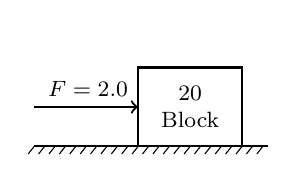
\begin{tikzpicture}[font=\footnotesize,xscale=0.66]
                \draw[white] (-2.0,1.5) -- (2.0,1.5);
                %% Force
                \draw[thick,->] (-2,0.5) -- (0,0.5)
                    node[pos=1.0,anchor=south east] {$F=\SI{2.0}{\newton}$};
                %% Block
                \draw[thick] (0,0) rectangle (2,1);
                \node[anchor=center,text width=3em,text centered]
                    at (1,0.5) {\SI{20}{\kilo\gram} Block};
                %% Floor
                \draw[thick] (-2,0) -- (2.5,0);
                \foreach \x in {-20,-18,...,25}
                    \draw[thin] (\x mm,0cm) -- ++ (220:0.15cm);
            \end{tikzpicture}
        }
        \wrongchoice{
            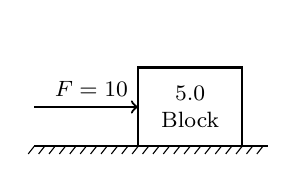
\begin{tikzpicture}[font=\footnotesize,xscale=0.66]
                \draw[white] (-2.0,1.5) -- (2.0,1.5);
                %% Force
                \draw[thick,->] (-2,0.5) -- (0,0.5)
                    node[pos=1.0,anchor=south east] {$F=\SI{10}{\newton}$};
                %% Block
                \draw[thick] (0,0) rectangle (2,1);
                \node[anchor=center,text width=3em,text centered]
                    at (1,0.5) {\SI{5.0}{\kilo\gram} Block};
                %% Floor
                \draw[thick] (-2,0) -- (2.5,0);
                \foreach \x in {-20,-18,...,25}
                    \draw[thin] (\x mm,0cm) -- ++ (220:0.15cm);
            \end{tikzpicture}
        }
        \wrongchoice{
            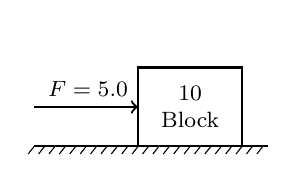
\begin{tikzpicture}[font=\footnotesize,xscale=0.66]
                \draw[white] (-2.0,1.5) -- (2.0,1.5);
                %% Force
                \draw[thick,->] (-2,0.5) -- (0,0.5)
                    node[pos=1.0,anchor=south east] {$F=\SI{5.0}{\newton}$};
                %% Block
                \draw[thick] (0,0) rectangle (2,1);
                \draw[thick] (0,0) rectangle (2,1);
                \node[anchor=center,text width=3em,text centered]
                    at (1,0.5) {\SI{10}{\kilo\gram} Block};
                %% Floor
                \draw[thick] (-2,0) -- (2.5,0);
                \foreach \x in {-20,-18,...,25}
                    \draw[thin] (\x mm,0cm) -- ++ (220:0.15cm);
            \end{tikzpicture}
        }
        \wrongchoice{
            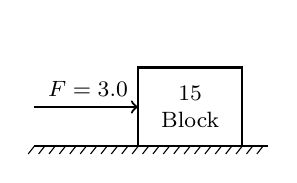
\begin{tikzpicture}[font=\footnotesize,xscale=0.66]
                \draw[white] (-2.0,1.5) -- (2.0,1.5);
                %% Force
                \draw[thick,->] (-2,0.5) -- (0,0.5)
                    node[pos=1.0,anchor=south east] {$F=\SI{3.0}{\newton}$};
                %% Block
                \draw[thick] (0,0) rectangle (2,1);
                \node[anchor=center,text width=3em,text centered]
                    at (1,0.5) {\SI{15}{\kilo\gram} Block};
                %% Floor
                \draw[thick] (-2,0) -- (2.5,0);
                \foreach \x in {-20,-18,...,25}
                    \draw[thin] (\x mm,0cm) -- ++ (220:0.15cm);
            \end{tikzpicture}
        }
    \end{choices}
    \end{multicols}
\end{question}
}

\element{nysed}{
\begin{question}{June2015-Q41}
    An object is in equilibrium. 
    Which force vector diagram could represent the force(s) acting on the object?
    \begin{multicols}{2}
    \begin{choices}
        \AMCboxDimensions{down=-1.3cm}
        \wrongchoice{
            \begin{tikzpicture}
                \draw[white] (-1.00,-1.5) rectangle (1.00,1.0);
                \node[draw,fill=white!90!black,circle,inner sep=0pt,minimum size=8pt] (A) at (0,0) {};
                \draw[thick,->] (A) -- ++ (270:1.414cm);
            \end{tikzpicture}
        }
        \wrongchoice{
            \begin{tikzpicture}
                \draw[white] (-1.00,-1.5) rectangle (1.00,1.0);
                \node[draw,fill=white!90!black,circle,inner sep=0pt,minimum size=8pt] (A) at (0,0) {};
                \draw[thick,->] (A) -- ++ (270:1.414cm);
                \draw[thick,->] (A) -- ++ (90:0.707cm);
            \end{tikzpicture}
        }
        \wrongchoice{
            \begin{tikzpicture}
                \draw[white] (-1.00,-1.5) rectangle (1.00,1.0);
                \node[draw,fill=white!90!black,circle,inner sep=0pt,minimum size=8pt] (A) at (0,0) {};
                \draw[thick,->] (A) -- ++ (0:0.707cm);
                \draw[thick,->] (A) -- ++ (180:0.707cm);
                \draw[thick,->] (A) -- ++ (270:1.414cm);
            \end{tikzpicture}
        }
        \correctchoice{
            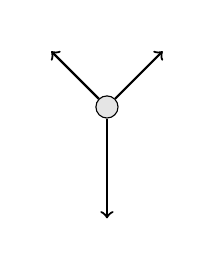
\begin{tikzpicture}
                \draw[white] (-1.00,-1.5) rectangle (1.00,1.0);
                \node[draw,fill=white!90!black,circle,inner sep=0pt,minimum size=8pt] (A) at (0,0) {};
                \draw[thick,->] (A) -- ++ (45:1.00cm);
                \draw[thick,->] (A) -- ++ (135:1.00cm);
                \draw[thick,->] (A) -- ++ (270:1.414cm);
            \end{tikzpicture}
        }
    \end{choices}
    \end{multicols}
\end{question}
}


%% Section June2014
%%--------------------
\element{nysed}{
\begin{question}{June2014-Q05}
    A baseball bat exerts a force of magnitude $F$ on a ball.
    If the mass of the bat is three times the mass of the ball,
        the magnitude of the force of the ball on the bat is:
    \begin{multicols}{2}
    \begin{choices}
      \correctchoice{$F$}
        \wrongchoice{$2F$}
        \wrongchoice{$3F$}
        \wrongchoice{$F/3$}
    \end{choices}
    \end{multicols}
\end{question}
}

\element{nysed}{
\begin{question}{June2014-Q08}
    A \SI{750}{\newton} person stands in an elevator that is accelerating downward.
    The upward force of the elevator floor on the person must be:
    \begin{choices}
      \correctchoice{less than \SI{750}{\newton}}
        \wrongchoice{equal to \SI{0}{\newton}}
        \wrongchoice{equal to \SI{750}{\newton}}
        \wrongchoice{greater than \SI{750}{\newton}}
    \end{choices}
\end{question}
}


%% Section June2013
%%--------------------
\element{nysed}{
\begin{question}{June2013-Q09}
    Which situation represents a person in equilibrium?
    \begin{choices}
        \wrongchoice{a child gaining speed while sliding a slide}
        \wrongchoice{a woman accelerating upward in an elevator}
      \correctchoice{a man standing on a bathroom scale}
        \wrongchoice{a teenager driving around a corner in his car}
    \end{choices}
\end{question}
}

\element{nysed}{
\begin{question}{June2013-Q10}
    A rock is thrown straight up into the air.
    At the highest point of the rock's path,
        the magnitude of the net force acting on the rock is:
    \begin{choices}
        \wrongchoice{less than the magnitude of the rock's weight, but greater than zero}
        \wrongchoice{greater than the magnitude of the rock's weight}
      \correctchoice{the same as the magnitude of the rock's weight}
        \wrongchoice{zero}
    \end{choices}
\end{question}
}

\element{nysed}{
\begin{question}{June2013-Q11}
    The diagram below shows a compressed spring between two carts initially at rest on a horizontal frictionless surface.
    Cart $A$ has a mass of \SI{2.0}{\kilo\gram} and cart $B$ has a mass of \SI{1.0}{\kilo\gram}.
    A string holds the carts together.
    \begin{center}
    \begin{tikzpicture}
        %% Ground
        \node[anchor=north,fill,pattern=north east lines,minimum width=8cm, minimum height=0.05cm] at (0,0) {};
        \draw (-4,0) -- (4,0);
        %% carts
        \node[draw,minimum width=2cm,minimum height=2em,anchor=south] (A) at (-2,0.3) {\SI{2}{\kilo\gram}};
        \node[draw,minimum width=1cm,minimum height=2em,anchor=south] (B) at (2,0.3) {\SI{1}{\kilo\gram}};
        \node[anchor=south] at (A.north) {$A$};
        \node[anchor=south] at (B.north) {$B$};
        %% wheels
        \draw[fill=white!90!black] (A.south west) ++(0:0.2cm) arc(90:-270:0.15);
        \draw[fill=white!90!black] (A.south east) ++(180:0.2cm) arc(90:-270:0.15);
        \draw[fill=white!90!black] (B.south west) ++(0:0.2cm) arc(90:-270:0.15);
        \draw[fill=white!90!black] (B.south east) ++(180:0.2cm) arc(90:-270:0.15);
        %% Spring
        \draw[decoration={aspect=0.2,segment length=1.5mm,amplitude=2mm,coil},decorate] (A.east) -- (B.west);
        \draw[thick] (A.north east) -- (B.north west);
    \end{tikzpicture}
    \end{center}
    The string is cut and the carts move apart.
    Compared to the magnitude of the force the spring exerts on cart $A$,
        the magnitude of the force the spring exerts on cart $B$ is:
    \begin{choices}
      \correctchoice{the same}
        \wrongchoice{half as great}
        \wrongchoice{twice as great}
        \wrongchoice{four times as great}
    \end{choices}
\end{question}
}

\element{nysed}{
\begin{question}{June2013-Q38}
    Four forces act concurrently on a block on a horizontal surface as shown in the diagram below.
    \begin{center}
    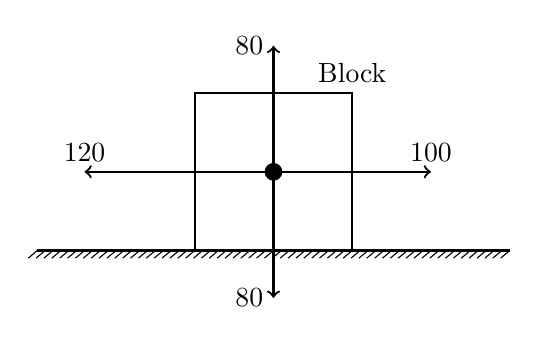
\begin{tikzpicture}
        \draw[fill] (0,0) circle (3pt);
        \draw[thick,->] (0,0) -- (0:2cm)
            node[anchor=south] {\SI{100}{\newton}};
        \draw[thick,->] (0,0) -- (90:1.6cm)
            node[anchor=east] {\SI{80}{\newton}};
        \draw[thick,->] (0,0) -- (180:2.4cm)
            node[anchor=south] {\SI{120}{\newton}};
        \draw[thick,->] (0,0) -- (270:1.6cm)
            node[anchor=east] {\SI{80}{\newton}};
        \draw[thick] (-1,-1) rectangle (1,1)
            node[anchor=south] {Block};
        \draw[thick] (-3,-1) -- (3,-1);
        \foreach \x in {-30,-29,...,30}
            \draw[thin] (\x mm,-1cm) -- ++ (220:0.15cm);
    \end{tikzpicture}
    \end{center}
    As a result of these forces, the block:
    \begin{choices}
        \wrongchoice{moves at constant speed to the right}
        \wrongchoice{moves at constant speed to the left}
        \wrongchoice{accelerates to the right}
      \correctchoice{accelerates to the left}
    \end{choices}
\end{question}
}

\element{nysed}{
\begin{question}{June2013-Q40}
    A \SI{4.0}{\kilo\gram} object is accelerated at \SI{3.0}{\meter\per\second\squared} north by an unbalanced force.
    The same unbalanced force acting on a \SI{2.0}{\kilo\gram} object will accelerate this object toward the north at:
    \begin{multicols}{2}
    \begin{choices}
        \wrongchoice{\SI{12}{\meter\per\second\squared}}
      \correctchoice{\SI{6.0}{\meter\per\second\squared}}
        \wrongchoice{\SI{3.0}{\meter\per\second\squared}}
        \wrongchoice{\SI{1.5}{\meter\per\second\squared}}
    \end{choices}
    \end{multicols}
\end{question}
}


%% Section June2012
%%--------------------
\element{nysed}{
\begin{question}{June2012-Q07}
    Which situation describes an object that has \emph{no} unbalanced force acting on it?
    \begin{choices}
        \wrongchoice{an apple in free fall}
        \wrongchoice{a satellite orbiting Earth}
      \correctchoice{a hockey puck moving at constant velocity}
        \wrongchoice{a laboratory cart moving down a frictionless \ang{30} incline}
    \end{choices}
\end{question}
}

\element{nysed}{
\begin{question}{June2012-Q12}
    A number of \SI{1.0}{\newton} horizontal forces are exerted on a block on a frictionless, horizontal surface.
    Which top-view diagram shows the forces producing the greatest magnitude of acceleration of the block?
    \begin{multicols}{2}
    \begin{choices}
        \AMCboxDimensions{down=-1.0cm}
        \correctchoice{
            \begin{tikzpicture}[font=\footnotesize]
                \draw[white] (-1.6,-1.6) rectangle (1.6,1.6);
                \node[draw,rectangle,minimum size=1cm,text centered,text width=1cm]
                    (B) at (0,0) {Top of Block};
                \draw[thick,->] (B.east) -- ++(0:1cm)
                    node[pos=0.5,anchor=south] {\SI{1.0}{\newton}};
                \draw[thick,->] (B.south) -- ++(270:1cm)
                    node[pos=0.5,anchor=east] {\SI{1.0}{\newton}};
            \end{tikzpicture}
        }
        \wrongchoice{
            \begin{tikzpicture}[font=\footnotesize]
                \draw[white] (-1.6,-1.6) rectangle (1.6,1.6);
                \node[draw,rectangle,minimum size=1cm,text centered,text width=1cm]
                    (B) at (0,0) {Top of Block};
                \draw[thick,->] (B.north) -- ++(90:1cm)
                    node[pos=0.5,anchor=east] {\SI{1.0}{\newton}};
                \draw[thick,->] (B.east) -- ++(0:1cm)
                    node[pos=0.5,anchor=south] {\SI{1.0}{\newton}};
                \draw[thick,->] (B.south) -- ++(270:1cm)
                    node[pos=0.5,anchor=east] {\SI{1.0}{\newton}};
                \draw[thick,->] (B.west) -- ++(180:1cm)
                    node[pos=0.5,anchor=south] {\SI{1.0}{\newton}};
            \end{tikzpicture}
        }
        \wrongchoice{
            \begin{tikzpicture}[font=\footnotesize]
                \draw[white] (-1.6,-1.6) rectangle (1.6,1.6);
                \node[draw,rectangle,minimum size=1cm,text centered,text width=1cm]
                    (B) at (0,0) {Top of Block};
                \draw[thick,->] (B.north) -- ++(90:1cm)
                    node[pos=0.5,anchor=east] {\SI{1.0}{\newton}};
                \draw[thick,->] (B.east) -- ++(0:1cm)
                    node[pos=0.5,anchor=south] {\SI{1.0}{\newton}};
                \draw[thick,->] (B.south) -- ++(270:1cm)
                    node[pos=0.5,anchor=east] {\SI{1.0}{\newton}};
            \end{tikzpicture}
        }
        \wrongchoice{
            \begin{tikzpicture}[font=\footnotesize]
                \draw[white] (-1.6,-1.6) rectangle (1.6,1.6);
                \node[draw,rectangle,minimum size=1cm,text centered,text width=1cm]
                    (B) at (0,0) {Top of Block};
                \draw[thick,->] (B.north) -- ++(90:1cm)
                    node[pos=0.5,anchor=east] {\SI{1.0}{\newton}};
                \draw[thick,->] (B.south) -- ++(270:1cm)
                    node[pos=0.5,anchor=east] {\SI{1.0}{\newton}};
            \end{tikzpicture}
        }
    \end{choices}
    \end{multicols}
\end{question}
}

%% NOTE: June2012-Q47 is too big


%% Section June2011
%%--------------------
\element{nysed}{
\begin{question}{June2011-Q06}
    A student is standing in an elevator that is accelerating downward.
    The force that the student exerts on the floor of the elevator must be:
    \begin{choices}
      \correctchoice{less than the weight of the student when at rest}
        \wrongchoice{greater than the weight of the student when at rest}
        \wrongchoice{less than the force of the floor on the student}
        \wrongchoice{greater than the force of the floor on the student}
    \end{choices}
\end{question}
}

\element{nysed}{
\begin{question}{June2011-Q12}
    Two forces act concurrently on an object on a horizontal,
        frictionless surface, as shown in the diagram below.
    \begin{center}
    \begin{tikzpicture}
        %% Ground
        \node[anchor=north,fill,pattern=north east lines,minimum width=8cm, minimum height=0.05cm] at (0,0) {};
        \draw (-4,0) -- (4,0);
        \node at (0,-0.5) {Horizontal, frictionless surface.};
        %% Object
        \node[draw,minimum size=1.6cm,anchor=south] (A) at (0,0) {Object};
        %% Forces
        \draw[thick,->] (A.west) -- ++(180:2) node[pos=0.5,anchor=south] {\SI{10}{\newton}};
        \draw[thick,->] (A.east) -- ++(0:1.2) node[pos=0.5,anchor=south] {\SI{6}{\newton}};
    \end{tikzpicture}
    \end{center}
    What additional force, when applied to the object,
        will establish equilibrium?
    \begin{choices}
        \wrongchoice{\SI{16}{\newton} toward the right}
        \wrongchoice{\SI{16}{\newton} toward the left}
        \wrongchoice{\SI{4}{\newton} toward the right}
      \correctchoice{\SI{4}{\newton} toward the left}
    \end{choices}
\end{question}
}

\element{nysed}{
\begin{question}{June2011-Q38}
    A \SI{75}{\kilo\gram} hockey player is skating across the ice at a speed of \SI{6.0}{\meter\per\second}.
    What is the magnitude of the average force required to stop the player in \SI{0.65}{\second}?
    \begin{multicols}{2}
    \begin{choices}
        \wrongchoice{\SI{120}{\newton}}
        \wrongchoice{\SI{290}{\newton}}
      \correctchoice{\SI{690}{\newton}}
        \wrongchoice{\SI{920}{\newton}}
    \end{choices}
    \end{multicols}
\end{question}
}


%% Section June2010
%%--------------------
\element{nysed}{
\begin{question}{June2010-Q04}
    A \SI{0.149}{\kilo\gram} baseball,
        initially moving at \SI{15}{\meter\per\second},
        is brought to rest in \SI{0.040}{\second} by a baseball glove on a catcher's hand.
    The magnitude of the average force exerted on the ball by the glove is:
    \begin{multicols}{2}
    \begin{choices}
        \wrongchoice{\SI{2.2}{\newton}}
        \wrongchoice{\SI{2.9}{\newton}}
        \wrongchoice{\SI{17}{\newton}}
      \correctchoice{\SI{56}{\newton}}
    \end{choices}
    \end{multicols}
\end{question}
}

\element{nysed}{
\begin{question}{June2010-Q05}
    Which body is in equilibrium?
    \begin{choices}
        \wrongchoice{A satellite moving around Earth in a circular orbit.}
        \wrongchoice{A cart rolling down a frictionless incline.}
        \wrongchoice{An apple falling freely toward the surface of Earth.}
      \correctchoice{A block sliding at constant velocity across a tabletop.}
    \end{choices}
\end{question}
}

\element{nysed}{
\begin{question}{June2010-Q08}
    A student pulls a \SI{60}{\newton} sled with a force having a magnitude of \SI{20}{\newton}.
    What is the magnitude of the force that the sled exerts on the student?
    \begin{multicols}{2}
    \begin{choices}
      \correctchoice{\SI{20}{\newton}}
        \wrongchoice{\SI{40}{\newton}}
        \wrongchoice{\SI{60}{\newton}}
        \wrongchoice{\SI{80}{\newton}}
    \end{choices}
    \end{multicols}
\end{question}
}

\element{nysed}{
\begin{question}{June2010-Q10}
    The diagram below shows a horizontal \SI{12}{\newton} force being applied to two blocks, $A$ and $B$, initially at rest on a horizontal, frictionless surface.
    Block $A$ has a mass of \SI{1.0}{\kilo\gram} and block $B$ has a mass of \SI{2.0}{\kilo\gram}.
    \begin{center}
    \begin{tikzpicture}[font=\footnotesize]
        %% Force
        \draw[thick,->] (-2,0.5) -- (0,0.5)
            node[above left] {$F=\SI{12}{\newton}$};
        %% Block A
        \draw[thick] (0,0) rectangle (1,1);
        \node[anchor=south] at (0.5,0.5) {$A$};
        \node[anchor=north] at (0.5,0.5) {\SI{1.0}{\kilo\gram}};
        %% Block B
        \draw[thick] (1,0) rectangle (2,2);
        \node[anchor=south] at (1.5,1) {$B$};
        \node[anchor=north] at (1.5,1) {\SI{2.0}{\kilo\gram}};
        %% Floor
        \draw[thick] (-3,0) -- (3,0);
        \foreach \x in {-30,-29,...,30}
            \draw[thin] (\x mm,0cm) -- ++ (220:0.15cm);
        \node[anchor=north] at (0,-0.15) {Frictionless surface};
    \end{tikzpicture}
    \end{center}
    The magnitude of the acceleration of block $B$ is:
    \begin{multicols}{2}
    \begin{choices}
        \wrongchoice{\SI{6.0}{\meter\per\second\squared}}
        \wrongchoice{\SI{2.0}{\meter\per\second\squared}}
        \wrongchoice{\SI{3.0}{\meter\per\second\squared}}
      \correctchoice{\SI{4.0}{\meter\per\second\squared}}
    \end{choices}
    \end{multicols}
\end{question}
}


%% Section June2009
%%--------------------
\element{nysed}{
\begin{question}{June2009-Q05}
    A \SI{25}{\newton} weight falls freely from rest from the roof of a building.
    What is the total distance the weight falls in the first \SI{1.0}{\second}?
    \begin{multicols}{2}
    \begin{choices}
        \wrongchoice{\SI{19.6}{\meter}}
        \wrongchoice{\SI{9.8}{\meter}}
      \correctchoice{\SI{4.9}{\meter}}
        \wrongchoice{\SI{2.5}{\meter}}
    \end{choices}
    \end{multicols}
\end{question}
}

\element{nysed}{
\begin{question}{June2009-Q09}
    A \SI{0.50}{\kilo\gram} cart is rolling at a speed of \SI{0.40}{\meter\per\second}.
    If the speed of the cart is doubled, the inertia of the cart is:
    \begin{multicols}{2}
    \begin{choices}
        \wrongchoice{halved}
        \wrongchoice{doubled}
        \wrongchoice{quadrupled}
      \correctchoice{unchanged}
    \end{choices}
    \end{multicols}
\end{question}
}

\element{nysed}{
\begin{question}{June2009-Q10}
    Two forces, $F_1$ and $F_2$, are applied to a block on a frictionless,
        horizontal surface as shown below.
    \begin{center}
    \begin{tikzpicture}[xscale=0.95]
        %% Force 1
        \draw[thick,->] (0,0.5) -- (-4,0.5)
            node[above right] {$F_1=\SI{12}{\newton}$};
        %% Force 2
        \draw[thick,->] (2,0.5) -- (2.667,0.5);
        \node[anchor=south west] at (2,0.5) {$F_2=\SI{2}{\newton}$};
        %% Block
        \draw[thick] (0,0) rectangle (2,1);
        \node[anchor=center] at (1,0.5) {Block};
        %% Floor
        \draw[thick] (-3,0) -- (3,0);
        \foreach \x in {-30,-29,...,30}
            \draw[thin] (\x mm,0cm) -- ++ (220:0.15cm);
        \node[anchor=north] at (0,-0.15) {Frictionless surface};
    \end{tikzpicture}
    \end{center}
    If the magnitude of the block's acceleration is \SI{2.0}{\meter\per\second\squared},
        what is the mass of the block?
    \begin{multicols}{2}
    \begin{choices}
        \wrongchoice{\SI{1}{\kilo\gram}}
      \correctchoice{\SI{5}{\kilo\gram}}
        \wrongchoice{\SI{6}{\kilo\gram}}
        \wrongchoice{\SI{7}{\kilo\gram}}
    \end{choices}
    \end{multicols}
\end{question}
}

\element{nysed}{
\begin{question}{June2009-Q12}
    What is the weight of a \SI{2.00}{\kilo\gram} object on the surface of Earth?
    \begin{multicols}{2}
    \begin{choices}
        \wrongchoice{\SI{4.91}{\newton}}
        \wrongchoice{\SI{2.00}{\newton}}
        \wrongchoice{\SI{9.81}{\newton}}
      \correctchoice{\SI{19.6}{\newton}}
    \end{choices}
    \end{multicols}
\end{question}
}

\element{nysed}{
\begin{question}{June2009-Q40}
    A motorcycle being driven on a dirt path hits a rock.
    Its \SI{60}{\kilo\gram} cyclist is project over the handlebars at \SI{20}{\meter\per\second} into a haystack.
    If the cyclist is brought to rest in \SI{0.50}{\second},
        the magnitude of the average force exerted on the cyclist by haystack is:
    \begin{multicols}{2}
    \begin{choices}
        \wrongchoice{\SI{6.0e1}{\newton}}
        \wrongchoice{\SI{5.9e2}{\newton}}
        \wrongchoice{\SI{1.2e3}{\newton}}
      \correctchoice{\SI{2.4e3}{\newton}}
    \end{choices}
    \end{multicols}
\end{question}
}


%% Section Jan2009
%%--------------------
\element{nysed}{
\begin{question}{Jan2009-Q01}
    A force of \SI{25}{\newton} east and a force of \SI{25}{\newton} west act concurrently on a \SI{5.0}{\kilo\gram} cart.
    What is the acceleration of the cart?
    \begin{multicols}{2}
    \begin{choices}
        \wrongchoice{\SI{1.0}{\meter\per\second\squared} west}
        \wrongchoice{\SI{0.20}{\meter\per\second\squared} east}
        \wrongchoice{\SI{5.0}{\meter\per\second\squared} east}
      \correctchoice{\SI{0}{\meter\per\second\squared}}
    \end{choices}
    \end{multicols}
\end{question}
}

\element{nysed}{
\begin{question}{Jan2009-Q03}
    What is the acceleration due to gravity at a location where a \SI{15.0}{\kilo\gram} mass weighs \SI{45.0}{\newton}?
    \begin{multicols}{2}
    \begin{choices}
        \wrongchoice{\SI{675}{\meter\per\second\squared}}
        \wrongchoice{\SI{9.81}{\meter\per\second\squared}}
      \correctchoice{\SI{3.0}{\meter\per\second\squared}}
        \wrongchoice{\SI{0.333}{\meter\per\second\squared}}
    \end{choices}
    \end{multicols}
\end{question}
}

\element{nysed}{
\begin{question}{Jan2009-Q38}
    Which graph best represents the motion of an object in equilibrium?
    \begin{multicols}{2}
    \begin{choices}
        \AMCboxDimensions{down=-2.5em}
        \correctchoice{
            \begin{tikzpicture}
                \begin{axis}[
                    axis y line=left,
                    axis x line=bottom,
                    axis line style={->},
                    xlabel={time},
                    xtick=\empty,
                    ylabel={displacement},
                    ytick=\empty,
                    xmin=0,xmax=11,
                    ymin=0,ymax=11,
                    width=1.0\columnwidth,
                ]
                \addplot[line width=1pt,domain=0:10]{x};
                \end{axis}
            \end{tikzpicture}
        }
        \wrongchoice{
            \begin{tikzpicture}
                \begin{axis}[
                    axis y line=left,
                    axis x line=bottom,
                    axis line style={->},
                    xlabel={time},
                    xtick=\empty,
                    ylabel={velocity},
                    ytick=\empty,
                    xmin=0,xmax=11,
                    ymin=0,ymax=11,
                    width=1.0\columnwidth,
                ]
                \addplot[line width=1pt,domain=0:10]{x};
                \end{axis}
            \end{tikzpicture}
        }
        \wrongchoice{
            \begin{tikzpicture}
                \begin{axis}[
                    axis y line=left,
                    axis x line=bottom,
                    axis line style={->},
                    xlabel={time},
                    xtick=\empty,
                    ylabel={displacement},
                    ytick=\empty,
                    xmin=0,xmax=11,
                    ymin=0,ymax=11,
                    width=1.0\columnwidth,
                ]
                \addplot[line width=1pt,domain=0:10]{0.1*x*x};
                \end{axis}
            \end{tikzpicture}
        }
        \wrongchoice{
            \begin{tikzpicture}
                \begin{axis}[
                    axis y line=left,
                    axis x line=bottom,
                    axis line style={->},
                    xlabel={time},
                    xtick=\empty,
                    ylabel={velocity},
                    ytick=\empty,
                    xmin=0,xmax=11,
                    ymin=0,ymax=11,
                    width=1.0\columnwidth,
                ]
                \addplot[line width=1pt,domain=0:10]{0.1*x*x};
                \end{axis}
            \end{tikzpicture}
        }
    \end{choices}
    \end{multicols}
\end{question}
}


%% Section Aug2008
%%--------------------
\element{nysed}{
\begin{question}{Aug2008-Q01}
    A net force of \SI{25}{\newton} is applied horizontally to a \SI{10}{\kilo\gram} block resting on a table.
    What is the magnitude of the acceleration of the block?
    \begin{multicols}{2}
    \begin{choices}
        \wrongchoice{\SI{0.0}{\meter\per\second\squared}}
        \wrongchoice{\SI{0.26}{\meter\per\second\squared}}
        \wrongchoice{\SI{0.40}{\meter\per\second\squared}}
      \correctchoice{\SI{2.5}{\meter\per\second\squared}}
    \end{choices}
    \end{multicols}
\end{question}
}

\element{nysed}{
\begin{question}{Aug2008-Q06}
    If the magnitude of the gravitational force of Earth on the Moon is $F$,
        the magnitude of the gravitational force of the Moon on Earth is:
    \begin{choices}
        \wrongchoice{smaller than $F$}
        \wrongchoice{larger than $F$}
      \correctchoice{equal to $F$}
    \end{choices}
\end{question}
}

\element{nysed}{
\begin{question}{Aug2008-Q07}
    Which term represents a scalar quantity?
    \begin{multicols}{2}
    \begin{choices}
      \correctchoice{distance}
        \wrongchoice{displacement}
        \wrongchoice{force}
        \wrongchoice{weight}
    \end{choices}
    \end{multicols}
\end{question}
}


%% Section June2008
%%--------------------
\element{nysed}{
\begin{question}{June2008-Q09}
    Which diagram represents a box in equilibrium?
    \begin{multicols}{2}
    \begin{choices}
        \AMCboxDimensions{down=-1.5cm}
        \wrongchoice{
            \begin{tikzpicture}
                \draw[draw=white] (-1.6,-1.6) rectangle (1.6,1.6);
                \node[draw,rectangle,minimum size=2em] (B) at (0,0) {Box};
                \draw[thick,<-] (B.east) -- ++(0:1.15cm) node[pos=0.5,anchor=south] {\SI{5}{\newton}};
                \draw[thick,<-] (B.west) -- ++(180:1.15cm) node[pos=0.5,anchor=south] {\SI{5}{\newton}};
                \draw[thick,->] (B.south) -- ++(270:1.15cm) node[pos=0.5,anchor=west] {\SI{5}{\newton}};
            \end{tikzpicture}
        }
        \correctchoice{
            \begin{tikzpicture}
                \draw[draw=white] (-1.6,-1.6) rectangle (1.6,1.6);
                \node[draw,rectangle,minimum size=2em] (B) at (0,0) {Box};
                \draw[thick,->] (B.north) -- ++(90:0.5cm) node[pos=1.0,anchor=south] {\SI{2}{\newton}};
                \draw[thick,->] (B.south) -- ++(270:0.5cm) node[pos=1.0,anchor=north] {\SI{2}{\newton}};
                \draw[thick,<-] (B.west) -- ++(180:1.15cm) node[pos=0.5,anchor=south] {\SI{5}{\newton}};
                \draw[thick,<-] (B.east) -- ++(0:1.15cm) node[pos=0.5,anchor=south] {\SI{5}{\newton}};
            \end{tikzpicture}
        }
        \wrongchoice{
            \begin{tikzpicture}
                \draw[draw=white] (-1.6,-1.6) rectangle (1.6,1.6);
                \node[draw,rectangle,minimum size=2em] (B) at (0,0) {Box};
                \draw[thick,<-] (B.west) -- ++(180:0.5cm) node[pos=1.0,anchor=east] {\SI{2}{\newton}};
                \draw[thick,<-] (B.east) -- ++(0:0.5cm) node[pos=1.0,anchor=west] {\SI{2}{\newton}};
                \draw[thick,->] (B.north) -- ++(90:0.5cm) node[pos=1.0,anchor=south] {\SI{2}{\newton}};
                \draw[thick,->] (B.south) -- ++(270:1.15cm) node[pos=0.5,anchor=west] {\SI{5}{\newton}};
            \end{tikzpicture}
        }
        \wrongchoice{
            \begin{tikzpicture}
                \draw[draw=white] (-1.6,-1.6) rectangle (1.6,1.6);
                \node[draw,rectangle,minimum size=2em] (B) at (0,0) {Box};
                \draw[thick,<-] (B.east) -- ++(0:0.72cm) node[pos=0.5,anchor=south west] {\SI{3}{\newton}};
                \draw[thick,<-] (B.south) -- ++(270:0.5cm) node[pos=1.0,anchor=north] {\SI{2}{\newton}};
                \draw[thick,<-] (B.west) -- ++(180:1.15cm) node[pos=0.5,anchor=south] {\SI{5}{\newton}};
            \end{tikzpicture}
        }
    \end{choices}
    \end{multicols}
\end{question}
}

\element{nysed}{
\begin{question}{June2008-Q15}
    A carpenter hits a nail with a hammer.
    Compared to the magnitude of the force the hammer exerts on the nail,
        the magnitude of the force the nail exerts on the hammer during contact is:
    \begin{choices}
        \wrongchoice{less}
        \wrongchoice{greater}
      \correctchoice{the same}
    \end{choices}
\end{question}
}

\element{nysed}{
\begin{question}{June2008-Q40}
    A \SI{25}{\newton} horizontal force northward and a \SI{35}{\newton} horizontal force southward act concurrently on a \SI{15}{\kilo\gram} object on a frictionless surface.
    What is the magnitude of the object's acceleration?
    \begin{multicols}{2}
    \begin{choices}
      \correctchoice{\SI{0.67}{\meter\per\second\squared}}
        \wrongchoice{\SI{1.7}{\meter\per\second\squared}}
        \wrongchoice{\SI{2.3}{\meter\per\second\squared}}
        \wrongchoice{\SI{4.0}{\meter\per\second\squared}}
    \end{choices}
    \end{multicols}
\end{question}
}


%% Section Jan2008
%%--------------------
\element{nysed}{
\begin{question}{Jan2008-Q12}
    If a \SI{65}{\kilo\gram} astronaut exerts a force with a magnitude of \SI{50}{\newton} on a satellite that she is repairing,
        the magnitude of the force that the satellite exerts on her is:
    \begin{choices}
        \wrongchoice{\SI{0}{\newton}}
        \wrongchoice{\SI{50}{\newton} less than her weight}
        \wrongchoice{\SI{50}{\newton} more than her weight}
      \correctchoice{\SI{50}{\newton}}
    \end{choices}
\end{question}
}

\element{nysed}{
\begin{question}{Jan2008-Q39}
    A bicycle and its rider have a combined mass of \SI{80}{\kilo\gram} and a speed of \SI{6.0}{\meter\per\second}.
    What is the magnitude of the average force needed to bring the bicycle and its rider to a stop in \SI{4.0}{\second}?
    \begin{multicols}{2}
    \begin{choices}
      \correctchoice{\SI{1.2e2}{\newton}}
        \wrongchoice{\SI{3.2e2}{\newton}}
        \wrongchoice{\SI{4.8e2}{\newton}}
        \wrongchoice{\SI{1.9e3}{\newton}}
    \end{choices}
    \end{multicols}
\end{question}
}


%% Section June2007
%%--------------------
\element{nysed}{
\begin{question}{June2007-Q03}
    A \SI{2.00}{\kilo\gram} object weighs \SI{19.6}{\newton} on Earth.
    If the acceleration due to gravity on Mars is \SI{3.71}{\meter\per\second\squared},
        what is the object's mass on Mars?
    \begin{multicols}{2}
    \begin{choices}
        \wrongchoice{\SI{2.64}{\kilo\gram}}
        \wrongchoice{\SI{19.6}{\newton}}
      \correctchoice{\SI{2.00}{\kilo\gram}}
        \wrongchoice{\SI{7.42}{\newton}}
    \end{choices}
    \end{multicols}
\end{question}
}

\element{nysed}{
\begin{question}{June2007-Q37}
    A force of \SI{1}{\newton} is equivalent to:
    \begin{multicols}{2}
    \begin{choices}
      \correctchoice{\SI{1}{\kilo\gram\meter\per\second\squared}}
        \wrongchoice{\SI{1}{\kilo\gram\meter\per\second}}
        \wrongchoice{\SI{1}{\kilo\gram\meter\squared\per\second}}
        \wrongchoice{\SI{1}{\kilo\gram\squared\meter\squared\per\second\squared}}
    \end{choices}
    \end{multicols}
\end{question}
}


%% Section Jan2007
%%--------------------
\element{nysed}{
\begin{question}{Jan2007-Q11}
    A \SI{0.15}{\kilo\gram} baseball moving at \SI{20}{\meter\per\second} is stopped by a catcher in \SI{0.010}{\second}.
    The average force stopping the ball is:
    \begin{multicols}{2}
    \begin{choices}
      \correctchoice{\SI{3.0e1}{\newton}}
        \wrongchoice{\SI{3.0e0}{\newton}}
        \wrongchoice{\SI{3.0e-2}{\newton}}
        \wrongchoice{\SI{3.0e2}{\newton}}
    \end{choices}
    \end{multicols}
\end{question}
}


%% Section June2006
%%--------------------
\element{nysed}{
\begin{question}{June2006-Q09}
    A \SI{60}{\kilo\gram} student jumps down from a laboratory counter.
    At the instant he lands on the floor his speed is \SI{3}{\meter\per\second}.
    If the student stops in \SI{0.2}{\second},
        what is the average force on the student?
    \begin{multicols}{2}
    \begin{choices}
      \correctchoice{\SI{9e2}{\newton}}
        \wrongchoice{\SI{1e-2}{\newton}}
        \wrongchoice{\SI{1e2}{\newton}}
        \wrongchoice{\SI{4}{\newton}}
    \end{choices}
    \end{multicols}
\end{question}
}

\element{nysed}{
\begin{question}{June2006-Q37}
    A \SI{2.0}{\kilo\gram} object is falling freely near Earth's surface.
    %% What is the magnitude of the gravitational force that Earth exerts on the object?
    %% NOTE: I prefer this wording
    What is the magnitude of the gravitational force that the \SI{2.0}{\kilo\gram} object exerts on Earth?
    \begin{multicols}{2}
    \begin{choices}
      \correctchoice{\SI{20.}{\newton}}
        \wrongchoice{\SI{2.0}{\newton}}
        \wrongchoice{\SI{0.20}{\newton}}
        \wrongchoice{\SI{0.0}{\newton}}
    \end{choices}
    \end{multicols}
\end{question}
}


%% Section Jan2006
%%--------------------
\element{nysed}{
\begin{question}{Jan2006-Q05}
    A \SI{2.0}{\kilo\gram} laboratory cart is sliding across a horizontal frictionless surface at a constant velocity of \SI{4.0}{\meter\per\second} east.
    What will be the cart's velocity after a \SI{6.0}{\newton} westward force acts on it for \SI{2.0}{\second}?
    \begin{multicols}{2}
    \begin{choices}
      \correctchoice{\SI{2.0}{\meter\per\second} west}
        \wrongchoice{\SI{2.0}{\meter\per\second} east}
        \wrongchoice{\SI{10.}{\meter\per\second} west}
        \wrongchoice{\SI{10.}{\meter\per\second} east}
    \end{choices}
    \end{multicols}
\end{question}
}

\newcommand{\nysedJanTwentyZeroSixQSeven}{
\begin{tikzpicture}[scale=0.75]
    %% glass and index card
    \draw (-3.2,0) -- (3.2,0);
    \draw (-2.8,0) -- (-2,-4) -- (2,-4) -- (2.8,0);
    %% megal disk
    \draw[fill=white!90!black] (-1,0) rectangle (1,0.2);
    %% labels
    \node[pin={30:Metal disk}] at (0,0.2) {};
    \node[pin={240:Index card}] at (-3,0) {};
    \node[pin={340:Glass}] at (2.0,-2) {};
\end{tikzpicture}
}

\element{nysed}{
\begin{question}{Jan2006-Q07}
    The diagram below shows a \SI{1.0}{\newton} metal disk resting on an index card that is balanced on top of a glass.
    \begin{center}
        \nysedJanTwentyZeroSixQSeven
    \end{center}
    What is the net force acting on the disk?
    \begin{multicols}{2}
    \begin{choices}
      \correctchoice{\SI{0}{\newton}}
        \wrongchoice{\SI{1.0}{\newton}}
        \wrongchoice{\SI{2.0}{\newton}}
        \wrongchoice{\SI{9.8}{\newton}}
    \end{choices}
    \end{multicols}
\end{question}
}

\element{nysed}{
\begin{question}{Jan2006-Q08}
    The diagram below shows a \SI{1.0}{\newton} metal disk resting on an index card that is balanced on top of a glass.
    \begin{center}
        \nysedJanTwentyZeroSixQSeven
    \end{center}
    When the index card is quickly pulled away from the glass in a horizontal direction,
        the disk falls straight down into the glass.
    This action is a result of the disk's
    \begin{multicols}{2}
    \begin{choices}
        \wrongchoice{inertia}
        \wrongchoice{charge}
        \wrongchoice{shape}
        \wrongchoice{temperature}
    \end{choices}
    \end{multicols}
\end{question}
}

\element{nysed}{
\begin{question}{Jan2006-Q11}
    A \SI{400}{\newton} girl standing on a dock exerts a force of \SI{100}{\newton} on a \SI{10000}{\newton} sailboat as she pushes is away from the dock.
    How much force does the sailboat exert on the girl?
    \begin{multicols}{2}
    \begin{choices}
      \correctchoice{\SI{100}{\newton}}
        \wrongchoice{\SI{25}{\newton}}
        \wrongchoice{\SI{400}{\newton}}
        \wrongchoice{\SI{10000}{\newton}}
    \end{choices}
    \end{multicols}
\end{question}
}


%% Section June2005
%%--------------------
\element{nysed}{
\begin{question}{June2005-Q01}
    A \SI{2.0}{\kilo\gram} body is initially traveling at a velocity of \SI{40}{\meter\per\second} east.
    If a constant force of \SI{10}{\newton} due east is applied to the body for \SI{5.0}{\second},
        the final speed of the body is:
    \begin{multicols}{2}
    \begin{choices}
      \correctchoice{\SI{65}{\meter\per\second}}
        \wrongchoice{\SI{130}{\meter\per\second}}
        \wrongchoice{\SI{15}{\meter\per\second}}
        \wrongchoice{\SI{25}{\meter\per\second}}
    \end{choices}
    \end{multicols}
\end{question}
}

\element{nysed}{
\begin{question}{June2005-Q09}
    A container of rocks with a mass of \SI{65.0}{\kilo\gram} is brought back from the moon's surface where the acceleration of gravity is \SI{1.62}{\meter\per\second\squared}.
    What is the weight of the container of rocks on Earth's surface?
    \begin{multicols}{2}
    \begin{choices}
      \correctchoice{\SI{638}{\newton}}
        \wrongchoice{\SI{394}{\newton}}
        \wrongchoice{\SI{105}{\newton}}
        \wrongchoice{\SI{65.0}{\newton}}
    \end{choices}
    \end{multicols}
\end{question}
}


%% Section Jan2005
%%--------------------
\element{nysed}{
\begin{question}{Jan2005-Q07}
    Two carts are pushed apart by an expanding spring,
        as shown in the diagram below.
    \begin{center}
    \begin{tikzpicture}
        %% Ground
        \node[anchor=north,fill,pattern=north east lines,minimum width=8cm, minimum height=0.05cm] at (0,0) {};
        \draw (-4,0) -- (4,0);
        %% Carts
        \node[draw,minimum height=0.8cm,minimum width=1.2cm,anchor=south] (L) at (-1.8,0.2) {\SI{1}{\kilo\gram}};
        \node[draw,minimum height=0.8cm,minimum width=1.8cm,anchor=south] (R) at (+1.8,0.2) {\SI{2}{\kilo\gram}};
        \draw[fill=white] (L.south west) ++(0:0.3) circle (0.2);
        \draw[fill=white] (L.south east) ++(180:0.3) circle (0.2);
        \draw[fill=white] (R.south west) ++(0:0.4) circle (0.2);
        \draw[fill=white] (R.south east) ++(180:0.4) circle (0.2);
        %% Spring
        \draw[decoration={aspect=0.2,segment length=1.5mm,amplitude=2mm,coil},decorate] (L.east) -- (R.west);
        %% Forces
        \draw[very thick,->] (L.west) -- ++(180:1cm);
        \draw[very thick,->] (R.east) -- ++(0:1cm);
    \end{tikzpicture}
    \end{center}
    If the average force on the \SI{1}{\kilo\gram} cart is \SI{1}{\newton},
        what is the average force on the \SI{2}{\kilo\gram} cart?
    \begin{multicols}{2}
    \begin{choices}
      \correctchoice{\SI{1}{\newton}}
        \wrongchoice{\SI{0.0}{\newton}}
        \wrongchoice{\SI{0.5}{\newton}}
        \wrongchoice{\SI{4}{\newton}}
    \end{choices}
    \end{multicols}
\end{question}
}


%% Section June2004
%%--------------------
\element{nysed}{
\begin{question}{June2004-Q03}
    A person is standing on a bathroom scale in an elevator car.
    If the scale reads a value greater than the weight of the person at rest,
        the elevator car could be moving:
    \begin{choices}
      \correctchoice{upward at increasing speed}
        \wrongchoice{upward at constant speed}
        \wrongchoice{downward at increasing speed}
        \wrongchoice{downward at constant speed}
    \end{choices}
\end{question}
}

\element{nysed}{
\begin{question}{June2004-Q10}
    A man is pushing a baby stroller.
    Compared to the magnitude of the force exerted on the stroller by a the man,
        the magnitude of the force exerted on the man by the stroller is:
    \begin{choices}
        \wrongchoice{zero}
        \wrongchoice{smaller, but greater than zero}
        \wrongchoice{larger}
      \correctchoice{the same}
    \end{choices}
\end{question}
}

\element{nysed}{
\begin{question}{June2004-Q36}
    A constant unbalanced force is applied to an object for a period of time.
    Which graph best represents the acceleration of the object as a function of elapsed time?
    \begin{multicols}{2}
    \begin{choices}
        \AMCboxDimensions{down=-2.5em}
        \correctchoice{
            \begin{tikzpicture}
                \begin{axis}[
                    axis y line=left,
                    axis x line=bottom,
                    axis line style={->},
                    xlabel={time},
                    xtick=\empty,
                    ylabel={acceleration},
                    ytick=\empty,
                    xmin=0,xmax=11,
                    ymin=0,ymax=11,
                    width=1.0\columnwidth,
                ]
                \addplot[line width=1pt,domain=0:10]{8};
                \end{axis}
            \end{tikzpicture}
        }
        \wrongchoice{
            \begin{tikzpicture}
                \begin{axis}[
                    axis y line=left,
                    axis x line=bottom,
                    axis line style={->},
                    xlabel={time},
                    xtick=\empty,
                    ylabel={acceleration},
                    ytick=\empty,
                    xmin=0,xmax=11,
                    ymin=0,ymax=11,
                    width=1.0\columnwidth,
                ]
                \addplot[line width=1pt,domain=0:10]{10-x};
                \end{axis}
            \end{tikzpicture}
        }
        \wrongchoice{
            \begin{tikzpicture}
                \begin{axis}[
                    axis y line=left,
                    axis x line=bottom,
                    axis line style={->},
                    xlabel={time},
                    xtick=\empty,
                    ylabel={acceleration},
                    ytick=\empty,
                    xmin=0,xmax=11,
                    ymin=0,ymax=11,
                    width=1.0\columnwidth,
                ]
                \addplot[line width=1pt,domain=0:10]{x};
                \end{axis}
            \end{tikzpicture}
        }
        \wrongchoice{
            \begin{tikzpicture}
                \begin{axis}[
                    axis y line=left,
                    axis x line=bottom,
                    axis line style={->},
                    xlabel={time},
                    xtick=\empty,
                    ylabel={acceleration},
                    ytick=\empty,
                    xmin=0,xmax=11,
                    ymin=0,ymax=11,
                    width=1.0\columnwidth,
                ]
                \addplot[line width=1pt,domain=0:10]{0.1*x*x};
                \end{axis}
            \end{tikzpicture}
        }
    \end{choices}
    \end{multicols}
\end{question}
}


%% Section Jan2004
%%--------------------
\element{nysed}{
\begin{question}{Jan2004-Q11}
    A \SI{40.}{\kilo\gram} mass is moving across a horizontal surface at \SI{4.0}{\meter\per\second}.
    What is the magnitude of the net force required to bring the mass to a stop in \SI{8.0}{\second}?
    \begin{multicols}{2}
    \begin{choices}
      \correctchoice{\SI{25}{\newton}}
        \wrongchoice{\SI{1.0}{\newton}}
        \wrongchoice{\SI{5.0}{\newton}}
        \wrongchoice{\SI{40.}{\newton}}
    \end{choices}
    \end{multicols}
\end{question}
}

\element{nysed}{
\begin{question}{Jan2004-Q38}
    A high school physics student is sitting in a seat reading this question.
        The magnitude of the force with which the seat is pushing up on the student to support him is closest to
    \begin{multicols}{2}
    \begin{choices}
      \correctchoice{\SI{600}{\newton}}
        \wrongchoice{\SI{0}{\newton}}
        \wrongchoice{\SI{60}{\newton}}
        \wrongchoice{\SI{6000}{\newton}}
        %% Added by jphafner
        %\wrongchoice{\SI{60000}{\newton}}
        %\wrongchoice{\SI{600000}{\newton}}
    \end{choices}
    \end{multicols}
\end{question}
}


%% Section June2003
%%--------------------
\element{nysed}{
\begin{question}{June2003-Q05}
    A man standing on a scale in an elevator notices that the scale reads \SI{30}{\newton} greater than his normal weight.
    Which type of movement of the elevator could cause this greater-than-normal reading?
    \begin{choices}
      \correctchoice{accelerating upward}
        \wrongchoice{accelerating downward}
        \wrongchoice{moving upward at constant speed}
        \wrongchoice{moving downward at constant speed}
    \end{choices}
\end{question}
}

\element{nysed}{
\begin{question}{June2003-Q08}
    A \SI{60}{\kilo\gram} skydiver is falling at a constant speed near the surface of Earth.
    The magnitude of the force of air friction acting on the skydiver is approximately:
    \begin{multicols}{2}
    \begin{choices}
      \correctchoice{\SI{600}{\newton}}
        \wrongchoice{\SI{60}{\newton}}
        \wrongchoice{\SI{6}{\newton}}
        \wrongchoice{\SI{0}{\newton}}
    \end{choices}
    \end{multicols}
\end{question}
}

\element{nysed}{
\begin{question}{June2003-Q11}
    When a \SI{12}{\newton} horizontal force is applied to a box on a horizontal tabletop, the box remains at rest.
    The force of static friction acting on the box is:
    \begin{choices}
        \wrongchoice{\SI{0}{\newton}}
        \wrongchoice{between \SI{0}{\newton} and \SI{12}{\newton}}
      \correctchoice{\SI{12}{\newton}}
        \wrongchoice{greater than \SI{12}{\newton}}
    \end{choices}
\end{question}
}

\element{nysed}{
\begin{question}{June2003-Q13}
    A \SI{1.5}{\kilo\gram} lab cart is accelerated uniformly from rest to a speed of \SI{2.0}{\meter\per\second} in \SI{0.5}{\second}.
    What is the magnitude of the force producing this acceleration?
    \begin{multicols}{2}
    \begin{choices}
      \correctchoice{\SI{6.0}{\newton}}
        \wrongchoice{\SI{3.0}{\newton}}
        \wrongchoice{\SI{0.70}{\newton}}
        \wrongchoice{\SI{1.5}{\newton}}
    \end{choices}
    \end{multicols}
\end{question}
}

\element{nysed}{
\begin{question}{June2003-Q46}
    Which graph best represents the motion of an object that is \emph{not} in equilibrium as it travels along a straight line?
    \begin{multicols}{2}
    \begin{choices}
        \AMCboxDimensions{down=-2.5em}
        \correctchoice{
            \begin{tikzpicture}
                \begin{axis}[
                    axis y line=left,
                    axis x line=bottom,
                    axis line style={->},
                    xlabel={time},
                    xtick=\empty,
                    ylabel={speed},
                    ytick=\empty,
                    xmin=0,xmax=11,
                    ymin=0,ymax=11,
                    width=1.0\columnwidth,
                ]
                \addplot[line width=1pt,domain=0:10]{x};
                \end{axis}
            \end{tikzpicture}
        }
        \wrongchoice{
            \begin{tikzpicture}
                \begin{axis}[
                    axis y line=left,
                    axis x line=bottom,
                    axis line style={->},
                    xlabel={time},
                    xtick=\empty,
                    ylabel={distance},
                    ytick=\empty,
                    xmin=0,xmax=11,
                    ymin=0,ymax=11,
                    width=1.0\columnwidth,
                ]
                \addplot[line width=1pt,domain=0:10]{x};
                \end{axis}
            \end{tikzpicture}
        }
        \wrongchoice{
            \begin{tikzpicture}
                \begin{axis}[
                    axis y line=left,
                    axis x line=bottom,
                    axis line style={->},
                    xlabel={time},
                    xtick=\empty,
                    ylabel={speed},
                    ytick=\empty,
                    xmin=0,xmax=11,
                    ymin=0,ymax=11,
                    width=1.0\columnwidth,
                ]
                \addplot[line width=1pt,domain=0:10]{8};
                \end{axis}
            \end{tikzpicture}
        }
        \wrongchoice{
            \begin{tikzpicture}
                \begin{axis}[
                    axis y line=left,
                    axis x line=bottom,
                    axis line style={->},
                    xlabel={time},
                    xtick=\empty,
                    ylabel={distance},
                    ytick=\empty,
                    xmin=0,xmax=11,
                    ymin=0,ymax=11,
                    width=1.0\columnwidth,
                ]
                \addplot[line width=1pt,domain=0:10]{8};
                \end{axis}
            \end{tikzpicture}
        }
    \end{choices}
    \end{multicols}
\end{question}
}


%% Section Jan2003
%%--------------------
\element{nysed}{
\begin{question}{Jan2003-Q01}
    The diagram below shows a worker using a rope to pull a car.
    \begin{center}
        %% too complex to tikz
        
\includegraphics[keepaspectratio,scale=0.75]{Jan2003-Q01}
    \end{center}
    The worker's pull on the handle of the cart can best be described as a force having:
    \begin{choices}
      \correctchoice{both magnitude and direction}
        \wrongchoice{magnitude, only}
        \wrongchoice{direction, only}
        \wrongchoice{neither magnitude nor direction}
    \end{choices}
\end{question}
}

\element{nysed}{
\begin{question}{Jan2003-Q04}
    The sum of all forces acting on a moving object is zero,
        the object will:
    \begin{choices}
      \correctchoice{continue moving with constant velocity}
        \wrongchoice{slow down and stop}
        \wrongchoice{change the direction of its motion}
        \wrongchoice{accelerate uniformly}
    \end{choices}
\end{question}
}

\element{nysed}{
\begin{question}{Jan2003-Q05}
    A net force of \SI{10}{\newton} accelerates an object at \SI{5.0}{\meter\per\second\squared}.
    What net force would be required to accelerate the same object at \SI{1.0}{\meter\per\second\squared}?
    \begin{multicols}{2}
    \begin{choices}
      \correctchoice{\SI{2.0}{\newton}}
        \wrongchoice{\SI{1.0}{\newton}}
        \wrongchoice{\SI{5.0}{\newton}}
        \wrongchoice{\SI{50}{\newton}}
    \end{choices}
    \end{multicols}
\end{question}
}

\element{nysed}{
\begin{question}{Jan2003-Q07}
    A \SI{1200}{\kilo\gram} car traveling at \SI{10}{\meter\per\second} hits a tree and is brought to rest in \SI{0.10}{\second}.
    What is the magnitude of the average force acting on the car to bring it to rest?
    \begin{multicols}{2}
    \begin{choices}
      \correctchoice{\SI{1.2e5}{\newton}}
        \wrongchoice{\SI{1.2e4}{\newton}}
        \wrongchoice{\SI{1.2e3}{\newton}}
        \wrongchoice{\SI{1.2e2}{\newton}}
    \end{choices}
    \end{multicols}
\end{question}
}

\element{nysed}{
\begin{question}{Jan2003-Q08}
    A spring scale reads \SI{20}{\newton} as it pulls a \SI{5.0}{\kilo\gram} mass across a table.
    What is the magnitude of the force exerted by the mass on the spring scale?
    \begin{multicols}{2}
    \begin{choices}
      \correctchoice{\SI{20}{\newton}}
        \wrongchoice{\SI{49}{\newton}}
        \wrongchoice{\SI{3.0}{\newton}}
        \wrongchoice{\SI{4.0}{\newton}}
    \end{choices}
    \end{multicols}
\end{question}
}

\element{nysed}{
\begin{question}{Jan2003-Q37}
    The diagram below shows a force of magnitude $F$ applied to a mass at angle $\theta$ relative to a horizontal frictionless surface.
    \begin{center}
    \begin{tikzpicture}[font=\footnotesize]
        %% Block
        \draw[thick] (-2,0) rectangle (0,1);
        \node[anchor=center] at (-1.0,0.5) {mass};
        %% Force 1
        \draw[dashed,thick] (0,0.5) -- (2.00,0.5)
            node[pos=0.5,anchor=north] {horizontal};
        \draw[thick,->] (0,0.5) -- ++(30:2)
            node[pos=0.5,anchor=south] {$F$};
        \draw[thick,dashed,<->] (1.0,0.5) arc (0:30:1.0)
            node[pos=0.5,anchor=west] {$\theta$};
        %% Floor
        \draw[thick] (-3,0) -- (3,0);
        \foreach \x in {-30,-29,...,30}
            \draw[thin] (\x mm,0cm) -- ++ (220:0.20cm);
        \node[anchor=north] at (0,-0.20) {Frictionless surface};
    \end{tikzpicture}
    \end{center}
    As angle $\theta$ is increased, the horizontal acceleration of the mass:
    \begin{choices}
      \correctchoice{decreases}
        \wrongchoice{increases}
        \wrongchoice{remains the same}
    \end{choices}
\end{question}
}


%% Section Aug2002
%%--------------------
\element{nysed}{
\begin{question}{Aug2002-Q01}
    A net force of \SI{25}{\newton} is applied horizontally to a \SI{10}{\kilo\gram} block resting on a table.
    What is the magnitude of the acceleration of the block?
    \begin{multicols}{2}
    \begin{choices}
        \wrongchoice{\SI{0.0}{\meter\per\second\squared}}
        \wrongchoice{\SI{0.26}{\meter\per\second\squared}}
        \wrongchoice{\SI{0.40}{\meter\per\second\squared}}
      \correctchoice{\SI{2.5}{\meter\per\second\squared}}
    \end{choices}
    \end{multicols}
\end{question}
}

\element{nysed}{
\begin{question}{Aug2002-Q06}
    If the magnitude of the gravitational force of Earth on the Moon is $F$,
        the magnitude of the gravitational force of the Moon on Earth is:
    \begin{choices}
        \wrongchoice{smaller than $F$}
        \wrongchoice{larger than $F$}
      \correctchoice{equal to $F$}
    \end{choices}
\end{question}
}

\element{nysed}{
\begin{question}{Aug2002-Q27}
    During a collision, an \SI{84}{\kilo\gram} driver of a car moving at \SI{24}{\meter\per\second} is brought to rest by an inflating air bag in \SI{1.2}{\second}.
    The magnitude of the force exerted on the driver by the air bag is approximately:
    \begin{multicols}{2}
    \begin{choices}
        \wrongchoice{\SI{7.0e1}{\newton}}
        \wrongchoice{\SI{8.2e2}{\newton}}
      \correctchoice{\SI{1.7e3}{\newton}}
        \wrongchoice{\SI{2.0e3}{\newton}}
    \end{choices}
    \end{multicols}
\end{question}
}

\element{nysed}{
\begin{question}{Aug2002-Q28}
    An apple weighing \SI{1}{\newton} on the surface of Earth has a mass of approximately:
    \begin{multicols}{2}
    \begin{choices}
      \correctchoice{\SI{e-1}{\kilo\gram}}
        \wrongchoice{\SI{e0}{\kilo\gram}}
        \wrongchoice{\SI{e1}{\kilo\gram}}
        \wrongchoice{\SI{e2}{\kilo\gram}}
    \end{choices}
    \end{multicols}
\end{question}
}

\element{nysed}{
\begin{question}{Aug2002-Q31}
    In which situation is the net force on the object equal to zero?
    \begin{choices}
        \wrongchoice{a satellite moving at constant speed around Earth in a circular orbit}
        \wrongchoice{an automobile braking to a stop}
      \correctchoice{a bicycle moving at constant speed on a straight, level road}
        \wrongchoice{a pitched baseball being hit by a bat}
    \end{choices}
\end{question}
}


%% Section June2002
%%--------------------
\element{nysed}{
\begin{question}{June2002-Q07}
    A \SI{70}{\kilo\gram} astronaut has a weight of \SI{560}{\newton} on the surface of planet Alpha.
    What is the acceleration due to gravity on planet Alpha?
    \begin{multicols}{2}
    \begin{choices}
        \wrongchoice{\SI{0.0}{\meter\per\second\squared}}
        \wrongchoice{\SI{8.0}{\meter\per\second\squared}}
        \wrongchoice{\SI{9.8}{\meter\per\second\squared}}
      \correctchoice{\SI{80}{\meter\per\second\squared}}
    \end{choices}
    \end{multicols}
\end{question}
}

\element{nysed}{
\begin{question}{June2002-Q10}
    The diagram below shows a horizontal \SI{8.0}{\newton} force applied to a \SI{4.0}{\kilo\gram} block on a frictionless table.
    \begin{center}
    \begin{tikzpicture}
        %% Block
        \draw[thick] (-2,0) rectangle (0,1);
        \node[anchor=center] at (-1.0,0.5) {\SI{4.0}{\kilo\gram}};
        %% Force 1
        \draw[thick,->] (0,0.5) -- (2.00,0.5)
            node[pos=1.0,anchor=south east] {$F=\SI{8.0}{\newton}$};
        %% Floor
        \draw[thick] (-3,0) -- (3,0);
        \foreach \x in {-30,-29,...,30}
            \draw[thin] (\x mm,0cm) -- ++ (220:0.20cm);
        \node[anchor=north] at (0,-0.20) {Frictionless surface};
    \end{tikzpicture}
    \end{center}
    What is the magnitude of the block's acceleration?
    \begin{multicols}{2}
    \begin{choices}
        \wrongchoice{\SI{0.50}{\meter\per\second\squared}}
      \correctchoice{\SI{2.0}{\meter\per\second\squared}}
        \wrongchoice{\SI{9.8}{\meter\per\second\squared}}
        \wrongchoice{\SI{32}{\meter\per\second\squared}}
    \end{choices}
    \end{multicols}
\end{question}
}

\newcommand{\nysedJuneTwentyZeroTwoQTwelve}{
\begin{tikzpicture}
    %% Ground
    \node[anchor=north,fill,pattern=north east lines,minimum width=8cm, minimum height=0.05cm] at (0,0) {};
    \draw (-4,0) -- (4,0);
    %% carts
    \node[draw,minimum width=2cm,minimum height=2em,anchor=south] (A) at (-2,0.3) {\SI{2}{\kilo\gram}};
    \node[draw,minimum width=1cm,minimum height=2em,anchor=south] (B) at (2,0.3) {\SI{1}{\kilo\gram}};
    \node[anchor=south] at (A.north) {$A$};
    \node[anchor=south] at (B.north) {$B$};
    %% wheels
    \draw[fill=white!90!black] (A.south west) ++(0:0.2cm) arc(90:-270:0.15);
    \draw[fill=white!90!black] (A.south east) ++(180:0.2cm) arc(90:-270:0.15);
    \draw[fill=white!90!black] (B.south west) ++(0:0.2cm) arc(90:-270:0.15);
    \draw[fill=white!90!black] (B.south east) ++(180:0.2cm) arc(90:-270:0.15);
    %% Spring
    \draw[decoration={aspect=0.2,segment length=1.5mm,amplitude=2mm,coil},decorate] (A.east) -- (B.west);
    \draw[thick] (A.north east) -- (B.north west);
\end{tikzpicture}
}

\element{nysed}{
\begin{question}{June2002-Q12}
    The diagram shows a compressed spring between two carts initially at rest on a horizontal frictionless surface.
    Cart $A$ has a mass of 2 kilograms and cart $B$ has a mass of \SI{1}{\kilo\gram}.
    A string holds the carts together.
    \begin{center}
        \nysedJuneTwentyZeroTwoQTwelve
    \end{center}
    What occurs when the string is cut and the carts move apart?
    \begin{choices}
      \correctchoice{The magnitude of the acceleration of cart $A$ is one-half the magnitude of the acceleration of cart $B$.}
        \wrongchoice{The length of time that the force acts on cart $A$ is twice the length of time the force acts on cart $B$.}
        \wrongchoice{The magnitude of the force exerted on cart $A$ is one-half the magnitude of the force exerted on cart $B$.}
        \wrongchoice{The magnitude of the impulse applied to cart $A$ is twice the magnitude of the impulse applied to cart $B$.}
    \end{choices}
\end{question}
}

\element{nysed}{
\begin{question}{June2002-Q13}
    The diagram shows a compressed spring between two carts initially at rest on a horizontal frictionless surface.
    Cart $A$ has a mass of 2 kilograms and cart $B$ has a mass of \SI{1}{\kilo\gram}.
    A string holds the carts together.
    \begin{center}
        \nysedJuneTwentyZeroTwoQTwelve
    \end{center}
    After the string is cut and the two carts move apart,
        the magnitude of which quantity is the same for both carts?
    \begin{multicols}{2}
    \begin{choices}
      \correctchoice{momentum}
        \wrongchoice{inertia}
        \wrongchoice{velocity}
        \wrongchoice{kinetic energy}
    \end{choices}
    \end{multicols}
\end{question}
}


%% Section Jan2002
%%--------------------
\element{nysed}{
\begin{question}{Jan2002-Q07}
    A \SI{4.0}{\kilo\gram} rock and a \SI{1.0}{\kilo\gram} stone fall freely from rest from a height of \SI{100}{\meter}.
    After they fall for \SI{2.0}{\second},
        the ratio of the rock's speed to the stone's speed is:
    \begin{multicols}{2}
    \begin{choices}
      \correctchoice{$1:1$}
        \wrongchoice{$1:2$}
        \wrongchoice{$2:1$}
        \wrongchoice{$4:1$}
    \end{choices}
    \end{multicols}
\end{question}
}

\element{nysed}{
\begin{question}{Jan2002-Q09}
    In the diagram below,
        a box is on a frictionless horizontal surface with forces $F_1$ and $F_2$ acting as shown.
    \begin{center}
    \begin{tikzpicture}
        %% Block
        \draw[thick] (-1,0) rectangle (1,1);
        \node[anchor=center] at (0,0.5) {Box};
        %% Force 1
        \draw[thick,->] (1,0.5) -- (3.00,0.5)
            node[pos=1.0,anchor=south east] {$F_1$};
        %% Force 2
        \draw[thick,->] (-1,0.5) -- (-3.00,0.5)
            node[pos=1.0,anchor=south west] {$F_2$};
        %% Floor
        \draw[thick] (-3,0) -- (3,0);
        \foreach \x in {-30,-28,...,30}
            \draw[thin] (\x mm,0cm) -- ++ (220:0.20cm);
        \node[anchor=north] at (0,-0.20) {Frictionless surface};
    \end{tikzpicture}
    \end{center}
    If the magnitude of $F_1$ is greater than the magnitude of $F_2$,
        then the box is:
    \begin{choices}
        \wrongchoice{moving at constant speed in the direction of $F_1$}
        \wrongchoice{moving at constant speed in the direction of $F_2$}
      \correctchoice{accelerating in the direction of $F_1$}
        \wrongchoice{accelerating in the direction of $F_2$}
    \end{choices}
\end{question}
}

\element{nysed}{
\begin{question}{Jan2002-Q11}
    Which pair of displacement ($d$) and velocity ($v$) graphs best represent the motion of an object on which the net force is zero?
    \begin{choices}
        \AMCboxDimensions{down=-2.5em}
        \correctchoice{
            \begin{tikzpicture}
                \begin{groupplot}[
                    axis lines=middle,
                    axis line style={->},
                    group style={group size=2 by 1},
                    xtick=\empty,
                    x label style={
                        at={(current axis.right of origin)},
                        anchor=west,
                        font=\normalsize,
                    },
                    xmin=0,xmax=10,
                    ytick=\empty,
                    y label style={
                        at={(current axis.above origin)},
                        anchor=south,
                        font=\normalsize,
                    },
                    ymin=0,ymax=10,
                    width=0.5\columnwidth,
                    ]
                    \nextgroupplot[
                        xlabel={$t$},
                        ylabel={$d$},
                    ] \addplot[line width=1pt,domain=0:10] {x};
                    \nextgroupplot[
                        xlabel={$t$},
                        ylabel={$v$},
                    ] \addplot[line width=1pt,domain=0:10] {8};
                \end{groupplot}
            \end{tikzpicture}
        }
        \wrongchoice{
            \begin{tikzpicture}
                \begin{groupplot}[
                    axis lines=middle,
                    axis line style={->},
                    group style={group size=2 by 1},
                    xtick=\empty,
                    x label style={
                        at={(current axis.right of origin)},
                        anchor=west,
                        font=\normalsize,
                    },
                    xmin=0,xmax=10,
                    ytick=\empty,
                    y label style={
                        at={(current axis.above origin)},
                        anchor=south,
                        font=\normalsize,
                    },
                    ymin=0,ymax=10,
                    width=0.5\columnwidth,
                    ]
                    \nextgroupplot[
                        xlabel={$t$},
                        ylabel={$d$},
                    ] \addplot[line width=1pt,domain=0:10] {0.1 * x * x};
                    \nextgroupplot[
                        xlabel={$t$},
                        ylabel={$v$},
                    ] \addplot[line width=1pt,domain=0:10] {x};
                \end{groupplot}
            \end{tikzpicture}
        }
        \wrongchoice{
            \begin{tikzpicture}
                \begin{groupplot}[
                    axis lines=middle,
                    axis line style={->},
                    group style={group size=2 by 1},
                    xtick=\empty,
                    x label style={
                        at={(current axis.right of origin)},
                        anchor=west,
                        font=\normalsize,
                    },
                    xmin=0,xmax=10,
                    ytick=\empty,
                    y label style={
                        at={(current axis.above origin)},
                        anchor=south,
                        font=\normalsize,
                    },
                    ymin=0,ymax=10,
                    width=0.5\columnwidth,
                    ]
                    \nextgroupplot[
                        xlabel={$t$},
                        ylabel={$d$},
                    ] \addplot[line width=1pt,domain=0:10] {x};
                    \nextgroupplot[
                        xlabel={$t$},
                        ylabel={$v$},
                    ] \addplot[line width=1pt,domain=0:10] {0.5*x};
                \end{groupplot}
            \end{tikzpicture}
        }
        \wrongchoice{
            \begin{tikzpicture}
                \begin{groupplot}[
                    axis lines=middle,
                    axis line style={->},
                    group style={group size=2 by 1},
                    xtick=\empty,
                    x label style={
                        at={(current axis.right of origin)},
                        anchor=west,
                        font=\normalsize,
                    },
                    xmin=0,xmax=10,
                    ytick=\empty,
                    y label style={
                        at={(current axis.above origin)},
                        anchor=south,
                        font=\normalsize,
                    },
                    ymin=0,ymax=10,
                    width=0.5\columnwidth,
                    ]
                    \nextgroupplot[
                        xlabel={$t$},
                        ylabel={$d$},
                    ] \addplot[line width=1pt,domain=0:10] {0.1 * x * x};
                    \nextgroupplot[
                        xlabel={$t$},
                        ylabel={$v$},
                    ] \addplot[line width=1pt,domain=0:10] {8};
                \end{groupplot}
            \end{tikzpicture}
        }
    \end{choices}
\end{question}
}

\element{nysed}{
\begin{question}{Jan2002-Q13}
    The magnitude of the force that a baseball bat exerts on a ball is \SI{50}{\newton}.
    The magnitude of the force that the ball exerts on the bat is:
    \begin{multicols}{2}
    \begin{choices}
        \wrongchoice{\SI{5.0}{\newton}}
        \wrongchoice{\SI{10}{\newton}}
      \correctchoice{\SI{50}{\newton}}
        \wrongchoice{\SI{250}{\newton}}
    \end{choices}
    \end{multicols}
\end{question}
}

\element{nysed}{
\begin{question}{Jan2002-Q16}
    What is an essential characteristic of an object in equilibrium?
    \begin{choices}
        \wrongchoice{zero velocity}
      \correctchoice{zero acceleration}
        \wrongchoice{zero potential energy}
        \wrongchoice{zero kinetic energy}
    \end{choices}
\end{question}
}


%% Section June2001
%%--------------------
\element{nysed}{
\begin{question}{June2001-Q07}
    In an automobile collision, a \SI{44}{\kilo\gram} passenger moving at \SI{15}{\meter\per\second} is brought to rest by an air bag during a \SI{0.10}{\second} time interval.
    What is the magnitude of the average force exerted on the passenger during this time?
    \begin{multicols}{2}
    \begin{choices}
        \wrongchoice{\SI{440}{\newton}}
        \wrongchoice{\SI{660}{\newton}}
        \wrongchoice{\SI{4400}{\newton}}
      \correctchoice{\SI{6600}{\newton}}
    \end{choices}
    \end{multicols}
\end{question}
}

\element{nysed}{
\begin{question}{June2001-Q08}
    A series of unbalanced forces was applied to each of two blocks, $A$ and $B$.
    The graphs below show the relationship between unbalanced force and acceleration for each block.
    \begin{center}
    \begin{tikzpicture}
        \begin{groupplot}[
            axis y line=left,
            axis x line=bottom,
            axis line style={->},
            group style={group size=2 by 1},
            xtick={0,1,2,3,4},
            xlabel={acceleration},
            x unit=\si{\meter\per\second\squared},
            xmin=0,xmax=4.5,
            ytick={0,1,2,3},
            ylabel={force},
            y unit=\si{\newton},
            ymin=0,ymax=3.5,
            width=0.5\columnwidth,
            ]
            \nextgroupplot[title={Block $A$}]
            \addplot[line width=1pt,domain=0:3.5] {x};
            \addplot[mark=*] coordinates {(1,1) (2,2) (3,3)};
            \nextgroupplot[title={Block $B$}]
            \addplot[line width=1pt,domain=0:2] {2*x};
            \addplot[mark=*] coordinates {(0.5,1) (1,2) (1.5,3)};
        \end{groupplot}
    \end{tikzpicture}
    \end{center}
    Compared to the mass of block $A$,
        the mass of block $B$ is:
    \begin{multicols}{2}
    \begin{choices}
        \wrongchoice{the same}
      \correctchoice{twice as great}
        \wrongchoice{half as great}
        \wrongchoice{four times as great}
    \end{choices}
    \end{multicols}
\end{question}
}

\element{nysed}{
\begin{question}{June2001-Q55}
    A mosquito flying over a highway strikes the windshield of a moving truck.
    Compared to the magnitude of the force of the truck on the mosquito during the collision,
        the magnitude of the force of the mosquito on the truck is:
    \begin{multicols}{3}
    \begin{choices}
        \wrongchoice{smaller}
        \wrongchoice{larger}
      \correctchoice{the same}
    \end{choices}
    \end{multicols}
\end{question}
}


%% Section Jan2001
%%--------------------
\element{nysed}{
\begin{question}{Jan2001-Q08}
    Which is a derived unit?
    \begin{multicols}{2}
    \begin{choices}
        \wrongchoice{meter (\si{\meter})}
        \wrongchoice{kilogram (\si{\kilo\gram})}
        \wrongchoice{second (\si{\kilo\gram})}
      \correctchoice{newton (\si{\newton})}
    \end{choices}
    \end{multicols}
\end{question}
}

\element{nysed}{
\begin{question}{Jan2001-Q13}
    A \SI{2.0}{\kilo\gram} mass weights \SI{10}{\newton} on planet $X$.
    The acceleration due to gravity on planet $X$ is approximately:
    \begin{multicols}{2}
    \begin{choices}
        \wrongchoice{\SI{0.20}{\meter\per\second\squared}}
      \correctchoice{\SI{5.0}{\meter\per\second\squared}}
        \wrongchoice{\SI{9.8}{\meter\per\second\squared}}
        \wrongchoice{\SI{20}{\meter\per\second\squared}}
    \end{choices}
    \end{multicols}
\end{question}
}


%% Section June2000
%%--------------------
\element{nysed}{
\begin{question}{June2000-Q12}
    Two forces are applied to a \SI{2.0}{\kilo\gram} block on a frictionless horizontal surface,
        as shown in the diagram below.
    [Vectors are drawn to scale]
    \begin{center}
    \begin{tikzpicture}
        %% Force 1
        \draw[thick,->] (-0,0.5) -- (-2.66,0.5)
            node[pos=1.0,anchor=south west] {$F_1=\SI{8}{\newton}$};
        %% Force 2
        \draw[thick,->] (2,0.5) -- (3.00,0.5)
            node[pos=0.0,anchor=south west] {$F_2=\SI{3}{\newton}$};
        %% Block
        \draw[thick] (0,0) rectangle (2,1);
        \node[anchor=center] at (1,0.5) {\SI{2.0}{\kilo\gram}};
        %% Floor
        \draw[thick] (-3,0) -- (3,0);
        \foreach \x in {-30,-29,...,30}
            \draw[thin] (\x mm,0cm) -- ++ (220:0.15cm);
        \node[anchor=north] at (0,-0.15) {Frictionless surface};
    \end{tikzpicture}
    \end{center}
    The acceleration of the block is:
    \begin{choices}
        \wrongchoice{\SI{1.5}{\meter\per\second\squared} to the right}
      \correctchoice{\SI{2.5}{\meter\per\second\squared} to the left}
        \wrongchoice{\SI{2.5}{\meter\per\second\squared} to the right}
        \wrongchoice{\SI{4.0}{\meter\per\second\squared} to the left}
    \end{choices}
\end{question}
}

\element{nysed}{
\begin{question}{June2000-Q13}
    A \SI{15}{\kilo\gram} mass weighs \SI{60}{\newton} on planet $X$.
    The mass is allowed to fall freely from rest near the surface of the planet.
    After falling for \SI{6.0}{\second},
        the acceleration of the mass is:
    \begin{multicols}{2}
    \begin{choices}
        \wrongchoice{\SI{0.25}{\meter\per\second\squared}}
        \wrongchoice{\SI{10}{\meter\per\second\squared}}
        \wrongchoice{\SI{24}{\meter\per\second\squared}}
      \correctchoice{\SI{4.0}{\meter\per\second\squared}}
    \end{choices}
    \end{multicols}
\end{question}
}

\element{nysed}{
\begin{question}{June2000-Q17}
    A \SI{2 400}{\kilo\gram} car is traveling at a speed of \SI{20}{\meter\per\second}.
    Compared to the magnitude of the force required to stop the car in \SI{12}{\second},
        the magnitude of the force required to stop the car in \SI{6}{\second} is:
    \begin{choices}
        \wrongchoice{half as great}
      \correctchoice{twice as great}
        \wrongchoice{the same}
        \wrongchoice{four times as great}
    \end{choices}
\end{question}
}


%% Section June1999
%%--------------------
\element{nysed}{
\begin{question}{June1999-Q04}
    A \SI{1.2e3}{\kilo\gram} car is accelerated uniformly from \SI{10}{\meter\per\second} to \SI{20}{\meter\per\second} in \SI{5.0}{\second}.
    What is the magnitude of the net force acting on the car during this \SI{5.0}{\second} interval?
    \begin{multicols}{2}
    \begin{choices}
      \correctchoice{\SI{2.4e3}{\newton}}
        \wrongchoice{\SI{4.8e3}{\newton}}
        \wrongchoice{\SI{7.2e3}{\newton}}
        \wrongchoice{\SI{1.2e4}{\newton}}
    \end{choices}
    \end{multicols}
\end{question}
}

\element{nysed}{
\begin{question}{June1999-Q09}
    The diagram below shows a student applying a \SI{10}{\newton} force to slide a piece of wood at constant speed across a horizontal surface.
    After the wood is cut in half,
        one piece is placed on top of the other, as shown.
    \begin{center}
    \begin{tikzpicture}
        %% NOTE: add picture
    \end{tikzpicture}
    \end{center}
    What is the magnitude of the force, $F$,
        required to slide the stacked wood at constant speed across the surface?
    \begin{multicols}{2}
    \begin{choices}
        \wrongchoice{\SI{40}{\newton}}
        \wrongchoice{\SI{20}{\newton}}
      \correctchoice{\SI{10}{\newton}}
        \wrongchoice{\SI{5.0}{\newton}}
    \end{choices}
    \end{multicols}
\end{question}
}

\element{nysed}{
\begin{question}{June1999-Q11}
    Which combination of fundamental units can be used to express the weight of an object?
    \begin{choices}
        \wrongchoice{kilogram per second (\si{\kilo\gram\per\second})}
        \wrongchoice{kilogram meter (\si{\kilo\gram\meter})}
        \wrongchoice{kilogram meter per second (\si{\kilo\gram\meter\per\second})}
      \correctchoice{kilogram meter per second squared (\si{\kilo\gram\meter\per\second\squared})}
    \end{choices}
\end{question}
}

\element{nysed}{
\begin{question}{June1999-Q15}
    The diagram below shows a child pulling a \SI{50}{\kilo\gram} friend on a sled by applying a \SI{300}{\newton} force on the sled rope at an angle of \ang{40} with the horizontal.
    \begin{center}
        %% NOTE: too complex for tikz
        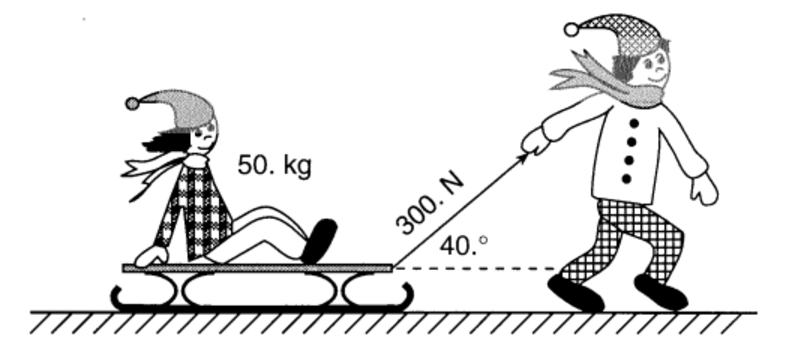
\includegraphics[keepaspectratio,scale=0.5]{June1999-Q15}
    \end{center}
    The vertical component of the \SI{300}{\newton} force is approximately:
    \begin{multicols}{2}
    \begin{choices}
        \wrongchoice{\SI{510}{\newton}}
        \wrongchoice{\SI{230}{\newton}}
      \correctchoice{\SI{190}{\newton}}
        \wrongchoice{\SI{32}{\newton}}
    \end{choices}
    \end{multicols}
\end{question}
}

\element{nysed}{
\begin{question}{June1999-Q17}
    A \SI{6.0}{\newton} force and a \SI{8}{\newton} force act concurrently on a box located on a frictionless horizontal surface.
    Which top-view diagram shows the forces producing the \emph{smallest} magnitude of acceleration of the box?
    \begin{multicols}{2}
    \begin{choices}[o]
        \footnotesize
        \AMCboxDimensions{down=-1.1cm}
        \correctchoice{
            \begin{tikzpicture}[scale=0.8]
                \draw[white!60!black,dashed] (-1.8,-2.0) rectangle (2.10,1.5);
                %% Block
                \node[draw,rectangle,minimum size=1cm,text centered,text width=1cm]
                    (B) at (0,0) {Top of Block};
                %% 8 Newton
                \draw[thick,->] (B.east) -- ++(0:1.33cm)
                    node[pos=1.0,anchor=south east] {\SI{8.0}{\newton}};
                %% 6 Newton
                \draw[thick,->] (B.west) -- ++(180:1.00cm)
                    node[pos=1.0,anchor=south west] {\SI{6.0}{\newton}};
            \end{tikzpicture}
        }
        \wrongchoice{
            \begin{tikzpicture}[scale=0.8]
                \draw[white!60!black,dashed] (-1.8,-2.0) rectangle (2.10,1.5);
                %% Block
                \node[draw,rectangle,minimum size=1cm,text centered,text width=1cm]
                    (B) at (0,0) {Top of Block};
                %% 8 Newton
                \draw[thick,->] (B.east) -- ++(0:1.33cm)
                    node[pos=1.0,anchor=south east] {\SI{8.0}{\newton}};
                %% 6 Newton
                \draw[thick,->] (B.south) -- ++(270:1.00cm)
                    node[pos=1.0,anchor=south west] {\SI{6.0}{\newton}};
            \end{tikzpicture}
        }
        \wrongchoice{
            \begin{tikzpicture}[scale=0.8]
                \draw[white!60!black,dashed] (-1.8,-2.0) rectangle (2.10,1.5);
                %% Block
                \node[draw,rectangle,minimum size=1cm,text centered,text width=1cm]
                    (B) at (0,0) {Top of Block};
                %% 8 Newton
                \draw[thick,->] (B.south) -- ++(270:1.33cm)
                    node[pos=1.0,anchor=south west] {\SI{8.0}{\newton}};
                %% 6 Newton
                \draw[thick,->] (B.west) -- ++(200:1.00cm)
                    node[pos=1.0,anchor=south west,rotate=20] {\SI{6.0}{\newton}};
            \end{tikzpicture}
        }
        \wrongchoice{
            \begin{tikzpicture}[scale=0.8]
                \draw[white!60!black,dashed] (-1.8,-2.0) rectangle (2.10,1.5);
                %% Block
                \node[draw,rectangle,minimum size=1cm,text centered,text width=1cm]
                    (B) at (0,0) {Top of Block};
                %% 8 Newton
                \draw[thick,->] (B.south)++(10pt,0) -- ++(270:1.33cm)
                    node[pos=0.5,anchor=west] {\SI{8.0}{\newton}};
                %% 6 Newton
                \draw[thick,->] (B.south)++(-10pt,0) -- ++(270:1.00cm)
                    node[pos=0.5,anchor=east] {\SI{6.0}{\newton}};
            \end{tikzpicture}
        }
    \end{choices}
    \end{multicols}
\end{question}
}


%% Section June1998
%%--------------------
\element{nysed}{
\begin{question}{June1998-Q08}
    A man weighs \SI{900}{\newton} standing on a scale in a stationary elevator.
    If some time later the reading on the scale is \SI{1200}{\newton},
        the elevator must be moving with:
    \begin{choices}
        \wrongchoice{constant acceleration downward}
        \wrongchoice{constant speed downward}
      \correctchoice{constant acceleration upward}
        \wrongchoice{constant speed upward}
    \end{choices}
\end{question}
}

\element{nysed}{
\begin{question}{June1998-Q09}
    Net force $F$ causes $m_1$ to accelerate at rate $a$.
    A net force of $3F$ causes mass $m_2$ to accelerate at rate $2a$.
    What is the ratio of mass $m_1$ to mass $m_2$?
    \begin{multicols}{2}
    \begin{choices}
        \wrongchoice{$1:3$}
      \correctchoice{$2:3$}
        \wrongchoice{$1:2$}
        \wrongchoice{$1:6$}
    \end{choices}
    \end{multicols}
\end{question}
}

\element{nysed}{
\begin{question}{June1998-Q13}
    A \SI{0.60}{\kilo\gram} softball initially at rest is hit with a bat.
    The ball is in contact with the bat for \SI{0.20}{\second} and leaves the bat with a speed of \SI{25}{\meter\per\second}.
    What is the magnitude of the average force exerted by the ball on the bat?
    \begin{multicols}{2}
    \begin{choices}
        \wrongchoice{\SI{8.3}{\newton}}
        \wrongchoice{\SI{15}{\newton}}
        \wrongchoice{\SI{3.0}{\newton}}
      \correctchoice{\SI{75}{\newton}}
    \end{choices}
    \end{multicols}
\end{question}
}

\element{nysed}{
\begin{question}{June1998-Q16}
    A person kicks a \SI{4.0}{\kilo\gram} door with a \SI{48}{\newton} force causing the door to accelerate at \SI{12}{\meter\per\second\squared}.
    What is the magnitude of the force exerted by the door on the person?
    \begin{multicols}{2}
    \begin{choices}
      \correctchoice{\SI{48}{\newton}}
        \wrongchoice{\SI{24}{\newton}}
        \wrongchoice{\SI{12}{\newton}}
        \wrongchoice{\SI{4.0}{\newton}}
    \end{choices}
    \end{multicols}
\end{question}
}


%% Section June1997
%%--------------------
\element{nysed}{
\begin{question}{June1997-Q05}
    A \SI{150}{\newton} force, $F_1$, and a \SI{200}{\newton} force,
        $F_2$, are applied simultaneously to the same point on a large crate resting on a frictionless, horizontal surface.
    Which diagram shows the forces positioned to give the crate the greatest acceleration?
    [Vectors are drawn to scale]
    \begin{multicols}{2}
    \begin{choices}
        \AMCboxDimensions{down=-0.25cm}
        \correctchoice{
            \begin{tikzpicture}[scale=0.75]
                \draw[white] (-2,-0.5) rectangle (2,2.33);
                %% Block
                \node[draw,rectangle,minimum size=0.8cm,anchor=south] (B) at (-0.5,0) {};
                %% F_1
                \draw[thick,->] (B.north east) -- ++(0:1.25)
                    node[pos=1.0,anchor=south east] {$F_1$};
                %% F_2
                \draw[thick,->] (B.east) -- ++(0:1.66)
                    node[pos=1.0,anchor=south] {$F_2$};
                %% Floor
                \draw[thick] (-2,0) -- (2,0);
                \node[anchor=north,pattern=north east lines,minimum width=3cm] at (0,0) {};
            \end{tikzpicture}
        }
        \wrongchoice{
            \begin{tikzpicture}[scale=0.75]
                \draw[white] (-2,-0.5) rectangle (2,2.33);
                %% Block
                \node[draw,rectangle,minimum size=0.8cm,anchor=south] (B) at (-0.5,0) {};
                %% F_1
                \draw[thick,<-] (B.north) -- ++(90:1.25)
                    node[pos=0.0,anchor=south east] {$F_1$};
                %% F_2
                \draw[thick,->] (B.east) -- ++(0:1.66)
                    node[pos=1.0,anchor=south east] {$F_2$};
                %% Floor
                \draw[thick] (-2,0) -- (2,0);
                \node[anchor=north,pattern=north east lines,minimum width=3cm] at (0,0) {};
            \end{tikzpicture}
        }
        \wrongchoice{
            \begin{tikzpicture}[scale=0.75]
                \draw[white] (-2,-0.5) rectangle (2,2.33);
                %% Block
                \node[draw,rectangle,minimum size=0.8cm,anchor=south] (B) at (-0.5,0) {};
                %% F_1
                \draw[thick,->] (B.north) -- ++(90:1.25)
                    node[pos=1.0,anchor=north east] {$F_1$};
                %% F_2
                \draw[thick,->] (B.east) -- ++(0:1.66)
                    node[pos=1.0,anchor=south east] {$F_2$};
                %% Floor
                \draw[thick] (-2,0) -- (2,0);
                \node[anchor=north,pattern=north east lines,minimum width=3cm] at (0,0) {};
            \end{tikzpicture}
        }
        \wrongchoice{
            \begin{tikzpicture}[scale=0.75]
                \draw[white] (-2,-0.5) rectangle (2,2.33);
                %% Block
                \node[draw,rectangle,minimum size=0.8cm,anchor=south] (B) at (-0.5,0) {};
                %% F_1
                \draw[thick,->] (B.west) -- ++(180:1.25)
                    node[pos=1.0,anchor=south west] {$F_1$};
                %% F_2
                \draw[thick,->] (B.east) -- ++(0:1.66)
                    node[pos=1.0,anchor=south east] {$F_2$};
                %% Floor
                \draw[thick] (-2,0) -- (2,0);
                \node[anchor=north,pattern=north east lines,minimum width=3cm] at (0,0) {};
            \end{tikzpicture}
        }
    \end{choices}
    \end{multicols}
\end{question}
}

\element{nysed}{
\begin{question}{June1997-Q11}
    The graph below shows the weight of three objects on planet $X$ as a function of their mass.
    \begin{center}
    \begin{tikzpicture}
        \begin{axis}[
            axis y line=left,
            axis x line=bottom,
            axis line style={->},
            ylabel={Weight},
            y unit=\si{\newton},
            ytick={0,100,200,300,400,500},
            xlabel={Mass},
            x unit=\si{\kilo\gram},
            xtick={0,25,50,75},
            xmin=0,xmax=77,
            ymin=0,ymax=510,
            grid=major,
            width=0.8\columnwidth,
            height=0.5\columnwidth,
            very thin,
        ]
        \addplot[line width=1pt,domain=0:75]{6.0* x};
        \addplot[mark=*] coordinates {(25,150) (50,300) (75,450)};
        \end{axis}
    \end{tikzpicture}
    \end{center}
    The acceleration due to gravity on planet $X$ is approximately:
    \begin{multicols}{2}
    \begin{choices}
        \wrongchoice{\SI{0.17}{\meter\per\second\squared}}
      \correctchoice{\SI{6.0}{\meter\per\second\squared}}
        \wrongchoice{\SI{9.8}{\meter\per\second\squared}}
        \wrongchoice{\SI{50}{\meter\per\second\squared}}
    \end{choices}
    \end{multicols}
\end{question}
}

\element{nysed}{
\begin{question}{June1997-Q12}
    What is the magnitude of the net force acting on a \SI{2.0e3}{\kilo\gram} car as it accelerates from rest to a speed of \SI{15}{\meter\per\second} in \SI{5.0}{\second}?
    \begin{multicols}{2}
    \begin{choices}
      \correctchoice{\SI{6.0e3}{\newton}}
        \wrongchoice{\SI{2.0e4}{\newton}}
        \wrongchoice{\SI{3.0e4}{\newton}}
        \wrongchoice{\SI{6.0e4}{\newton}}
    \end{choices}
    \end{multicols}
\end{question}
}


%% Section June1996
%%--------------------
\element{nysed}{
\begin{question}{June1996-Q07}
    A \SI{0.4}{\kilo\gram} rock and a \SI{1.0}{\kilo\gram} stone fall freely from rest from a height of \SI{100}{\meter}.
    After they fall for \SI{2.0}{\second},
        the ratio of the rock's speed to the stone's speed is:
    \begin{multicols}{2}
    \begin{choices}
      \correctchoice{$1:1$}
        \wrongchoice{$2:1$}
        \wrongchoice{$1:2$}
        \wrongchoice{$4:1$}
    \end{choices}
    \end{multicols}
\end{question}
}

%\element{nysed}{
%\begin{question}{June1996-Q09}
%    The diagram below shows a person exerting a \SI{300}{\newton} force on the handle of a shovel that makes an angle of \ang{60} with the horizontal ground.
%    \begin{center}
%        %% NOTE: picture of a person holding a shovel
%    \end{center}
%    The component of the \SI{300}{\newton} force that acts perpendicular to the ground is approximately:
%    \begin{multicols}{2}
%    \begin{choices}
%        \wrongchoice{\SI{150}{\newton}}
%      \correctchoice{\SI{260}{\newton}}
%        \wrongchoice{\SI{300}{\newton}}
%        \wrongchoice{\SI{350}{\newton}}
%    \end{choices}
%    \end{multicols}
%\end{question}
%}

\element{nysed}{
\begin{question}{June1996-Q10}
    Which graph best represents the motion of an object that has \emph{no} unbalanced force acting on it?
    \begin{multicols}{2}
    \begin{choices}
        \AMCboxDimensions{down=-2.5em}
        \correctchoice{
            \begin{tikzpicture}
                \begin{axis}[
                    axis y line=left,
                    axis x line=bottom,
                    axis line style={->},
                    xlabel={time},
                    xtick=\empty,
                    ylabel={displacement},
                    ytick=\empty,
                    xmin=0,xmax=11,
                    ymin=0,ymax=11,
                    width=1.0\columnwidth,
                ]
                \addplot[line width=1pt,domain=0:10]{0.1*x*x};
                \end{axis}
            \end{tikzpicture}
        }
        \wrongchoice{
            \begin{tikzpicture}
                \begin{axis}[
                    axis y line=left,
                    axis x line=bottom,
                    axis line style={->},
                    xlabel={time},
                    xtick=\empty,
                    ylabel={acceleration},
                    ytick=\empty,
                    xmin=0,xmax=11,
                    ymin=0,ymax=11,
                    width=1.0\columnwidth,
                ]
                \addplot[line width=1pt,domain=0:10]{x};
                \end{axis}
            \end{tikzpicture}
        }
        \wrongchoice{
            \begin{tikzpicture}
                \begin{axis}[
                    axis y line=left,
                    axis x line=bottom,
                    axis line style={->},
                    xlabel={time},
                    xtick=\empty,
                    ylabel={momentum},
                    ytick=\empty,
                    xmin=0,xmax=11,
                    ymin=0,ymax=11,
                    width=1.0\columnwidth,
                ]
                \addplot[line width=1pt,domain=0:10]{x};
                \end{axis}
            \end{tikzpicture}
        }
        \wrongchoice{
            \begin{tikzpicture}
                \begin{axis}[
                    axis y line=left,
                    axis x line=bottom,
                    axis line style={->},
                    xlabel={time},
                    xtick=\empty,
                    ylabel={velocity},
                    ytick=\empty,
                    xmin=0,xmax=11,
                    ymin=0,ymax=11,
                    width=1.0\columnwidth,
                ]
                \addplot[line width=1pt,domain=0:10]{0.1*x*x};
                \end{axis}
            \end{tikzpicture}
        }
    \end{choices}
    \end{multicols}
\end{question}
}

\element{nysed}{
\begin{question}{June1996-Q12}
    Two forces are applied to a \SI{2.0}{\kilo\gram} block on a frictionless,
        horizontal surface, as shown in the diagram below.
    \begin{center}
    \begin{tikzpicture}
        %% Force 1
        \draw[thick,->] (-2.0,0.5) -- (-2.75,0.5)
            node[pos=0.0,anchor=south east] {$F_1=\SI{2}{\newton}$};
        %% Force 2
        \draw[thick,->] (0,0.5) -- (3.0,0.5)
            node[pos=1.0,anchor=south east] at (2,0.5) {$F_2=\SI{8}{\newton}$};
        %% Block
        \draw[thick] (0,0) rectangle (-2,1);
        \node[anchor=center] at (-1,0.5) {\SI{2.0}{\kilo\gram}};
        %% Floor
        \draw[thick] (-3,0) -- (3,0);
        \node[anchor=north,minimum width=6cm,pattern=north east lines] at (0,0) {};
        \node[anchor=north,yshift=-1em] at (0,0) {Frictionless surface};
    \end{tikzpicture}
    \end{center}
    The acceleration of the block is:
    \begin{choices}
        \wrongchoice{\SI{5.0}{\meter\per\second\squared} to the right}
        \wrongchoice{\SI{5.0}{\meter\per\second\squared} to the left}
      \correctchoice{\SI{3.0}{\meter\per\second\squared} to the right}
        \wrongchoice{\SI{3.0}{\meter\per\second\squared} to the left}
    \end{choices}
\end{question}
}

\element{nysed}{
\begin{question}{June1996-Q13}
    Compared to the inertia of a \SI{0.10}{\kilo\gram} steel ball,
        the inertia of a \SI{0.20}{\kilo\gram} styrofoam ball is:
    \begin{multicols}{2}
    \begin{choices}
        \wrongchoice{one-half as great}
      \correctchoice{twice as great}
        \wrongchoice{the same}
        \wrongchoice{four times as great}
    \end{choices}
    \end{multicols}
\end{question}
}

\element{nysed}{
\begin{question}{June1996-Q15}
    As shown in the diagram below,
        an inflated balloon released from rest move horizontally with velocity $v$.
    \begin{center}
    \begin{tikzpicture}
        %% balloon
        \draw (0,1ex) to[out=0,in=180] (2,1) arc (90:-90:1) to[out=180,in=0] (0,-1ex);
        \draw[thick] (0,0) circle (0.25ex and 1ex);
        \node[anchor=center] at (2,0) {Balloon};
        \draw[thick,->] (1.5,1.25) -- ++(0:1) node[pos=0.5,anchor=south] {$v$};
        %% Air
        \foreach \x in {1,2,...,50} \fill ({-0.5 - 1*rnd},{0.25*rand}) circle (0.5pt);
        \node[anchor=south] at (-1,0.5) {air};
        \draw[thick,->] (-0.25,0) -- (180:2);
    \end{tikzpicture}
    \end{center}
    The velocity of the balloon is most likely cause by:
    \begin{choices}
      \correctchoice{action-reaction}
        \wrongchoice{centripetal force}
        \wrongchoice{gravitational attraction}
        \wrongchoice{rolling friction}
    \end{choices}
\end{question}
}


%% Section June1995
%%--------------------
\element{nysed}{
\begin{question}{June1995-Q07}
    Which combination of concurrent forces could \emph{not} produce equilibrium?
    \begin{choices}
      \correctchoice{\SI{10}{\newton}, \SI{20}{\newton}, and \SI{50}{\newton}}
        \wrongchoice{\SI{20}{\newton}, \SI{30}{\newton}, and \SI{50}{\newton}}
        \wrongchoice{\SI{30}{\newton}, \SI{40}{\newton}, and \SI{50}{\newton}}
        \wrongchoice{\SI{40}{\newton}, \SI{40}{\newton}, and \SI{50}{\newton}}
    \end{choices}
\end{question}
}

\element{nysed}{
\begin{question}{June1995-Q08}
    A \SI{60}{\kilo\gram} astronaut weighs \SI{96}{\newton} on the surface of the Moon.
    The acceleration due to gravity on the Moon is:
    \begin{multicols}{2}
    \begin{choices}
        \wrongchoice{\SI{0.0}{\meter\per\second\squared}}
      \correctchoice{\SI{1.6}{\meter\per\second\squared}}
        \wrongchoice{\SI{4.9}{\meter\per\second\squared}}
        \wrongchoice{\SI{9.8}{\meter\per\second\squared}}
    \end{choices}
    \end{multicols}
\end{question}
}

\element{nysed}{
\begin{question}{June1995-Q11}
    A student weighing \SI{500}{\newton} stands on a spring scale in an elevator.
    If the scale reads \SI{520}{\newton}, the elevator must be:
    \begin{choices}
      \correctchoice{accelerating upward}
        \wrongchoice{accelerating downward}
        \wrongchoice{moving upward at constant speed}
        \wrongchoice{moving downward at constant speed}
    \end{choices}
\end{question}
}

\element{nysed}{
\begin{question}{June1995-Q52}
    As the angle between a force and level ground decreases from \ang{60} to \ang{30},
        the vertical component of the force:
    \begin{choices}
      \correctchoice{decreases}
        \wrongchoice{increases}
        \wrongchoice{remains the same}
    \end{choices}
\end{question}
}

\element{nysed}{
\begin{question}{June1995-Q53}
    In a baseball game,
        a batter hits a ball for a home run.
    Compared to the magnitude of the impulse imparted to the ball,
        the magnitude of the impulse imparted to the bat is:
    \begin{multicols}{3}
    \begin{choices}
        \wrongchoice{less}
        \wrongchoice{greater}
      \correctchoice{the same}
    \end{choices}
    \end{multicols}
\end{question}
}


%% Section June1994
%%--------------------
\element{nysed}{
\begin{question}{June1994-Q02}
    Which two graphs represent the motion of an object on which the net force is zero?
    \begin{choices}
        \AMCboxDimensions{down=-2.5em}
        \wrongchoice{
            \begin{tikzpicture}
                \begin{groupplot}[
                        axis y line=left,
                        axis x line=bottom,
                        axis line style={->},
                        group style={group size=2 by 1},
                        xtick=\empty,
                        ytick=\empty,
                        width=0.5\columnwidth,
                    ]
                    \nextgroupplot[
                        xlabel={time},
                        ylabel={distance},
                        xmin=0,xmax=11,
                        ymin=0,ymax=11,
                    ] \addplot[line width=1pt,domain=0:10] {x};
                    \nextgroupplot[
                        xlabel={time},
                        ylabel={speed},
                        xmin=0,xmax=11,
                        ymin=0,ymax=11,
                    ] \addplot[line width=1pt,domain=0:10] {0.5*x};
                \end{groupplot}
            \end{tikzpicture}
        }
        %% ANS is 2
        \correctchoice{
            \begin{tikzpicture}
                \begin{groupplot}[
                        axis y line=left,
                        axis x line=bottom,
                        axis line style={->},
                        group style={group size=2 by 1},
                        xtick=\empty,
                        ytick=\empty,
                        width=0.5\columnwidth,
                    ]
                    \nextgroupplot[
                        xlabel={time},
                        ylabel={distance},
                        xmin=0,xmax=11,
                        ymin=0,ymax=11,
                    ] \addplot[line width=1pt,domain=0:10] {x};
                    \nextgroupplot[
                        xlabel={time},
                        ylabel={speed},
                        xmin=0,xmax=11,
                        ymin=0,ymax=11,
                    ] \addplot[line width=1pt,domain=0:10] {7};
                \end{groupplot}
            \end{tikzpicture}
        }
        \wrongchoice{
            \begin{tikzpicture}
                \begin{groupplot}[
                        axis y line=left,
                        axis x line=bottom,
                        axis line style={->},
                        group style={group size=2 by 1},
                        xtick=\empty,
                        ytick=\empty,
                        width=0.5\columnwidth,
                    ]
                    \nextgroupplot[
                        xlabel={time},
                        ylabel={distance},
                        xmin=0,xmax=11,
                        ymin=0,ymax=11,
                    ] \addplot[line width=1pt,domain=0:10] {0.1*x*x};
                    \nextgroupplot[
                        xlabel={time},
                        ylabel={speed},
                        xmin=0,xmax=11,
                        ymin=0,ymax=11,
                    ] \addplot[line width=1pt,domain=0:10] {0.5*x};
                \end{groupplot}
            \end{tikzpicture}
        }
        \wrongchoice{
            \begin{tikzpicture}
                \begin{groupplot}[
                        axis y line=left,
                        axis x line=bottom,
                        axis line style={->},
                        group style={group size=2 by 1},
                        xtick=\empty,
                        ytick=\empty,
                        width=0.5\columnwidth,
                    ]
                    \nextgroupplot[
                        xlabel={time},
                        ylabel={distance},
                        xmin=0,xmax=11,
                        ymin=0,ymax=11,
                    ] \addplot[line width=1pt,domain=0:10] {0.1*x*x};
                    \nextgroupplot[
                        xlabel={time},
                        ylabel={speed},
                        xmin=0,xmax=11,
                        ymin=0,ymax=11,
                    ] \addplot[line width=1pt,domain=0:10] {7};
                \end{groupplot}
            \end{tikzpicture}
        }
    \end{choices}
\end{question}
}

\element{nysed}{
\begin{question}{June1994-Q12}
    A net force of \SI{5.0e2}{\newton} causes an object to accelerated at a rate of \SI{5.0}{\meter\per\second\squared}.
    What is the mass of the object?
    \begin{multicols}{2}
    \begin{choices}
      \correctchoice{\SI{1.0e2}{\kilo\gram}}
        \wrongchoice{\SI{2.0e-1}{\kilo\gram}}
        \wrongchoice{\SI{6.0e2}{\kilo\gram}}
        \wrongchoice{\SI{2.5e3}{\kilo\gram}}
    \end{choices}
    \end{multicols}
\end{question}
}

\element{nysed}{
\begin{question}{June1994-Q14}
    The mass of a space shuttle is approximately \SI{2.0e6}{\kilo\gram}.
    During lift-off, the net force on the shuttle is \SI{1.0e7}{\newton} directed upward.
    What is the speed of the shuttle \SI{10}{\second} after lift-off?
    [Neglect air resistance and the mass change of the shuttle.]
    \begin{multicols}{2}
    \begin{choices}
        \wrongchoice{\SI{5.0e0}{\meter\per\second}}
      \correctchoice{\SI{5.0e1}{\meter\per\second}}
        \wrongchoice{\SI{5.0e2}{\meter\per\second}}
        \wrongchoice{\SI{5.0e3}{\meter\per\second}}
    \end{choices}
    \end{multicols}
\end{question}
}


%% Section June1990
%%--------------------
\element{nysed}{
\begin{question}{June1990-Q08}
    A force of \SI{6.0}{\newton} north and a force of \SI{8.0}{\newton} east act concurrently on an object.
    The magnitude of the resultant of the two forces is:
    \begin{multicols}{2}
    \begin{choices}
        \wrongchoice{\SI{1.3}{\newton}}
        \wrongchoice{\SI{2.0}{\newton}}
      \correctchoice{\SI{10}{\newton}}
        \wrongchoice{\SI{14}{\newton}}
    \end{choices}
    \end{multicols}
\end{question}
}

\element{nysed}{
\begin{question}{June1990-Q10}
    A \SI{50.0}{\kilo\gram} object in outer space is attracted to a nearby planet with a net force of \SI{400}{\newton}.
    What is the magnitude of the object's acceleration?
    \begin{multicols}{2}
    \begin{choices}
      \correctchoice{\SI{8.00}{\meter\per\second\squared}}
        \wrongchoice{\SI{9.81}{\meter\per\second\squared}}
        \wrongchoice{\SI{78.4}{\meter\per\second\squared}}
        \wrongchoice{\SI{2 000}{\meter\per\second\squared}}
    \end{choices}
    \end{multicols}
\end{question}
}


%% Section June1989
%%--------------------
\element{nysed}{
\begin{question}{June1989-Q05}
    The diagram below shows a graph of distance as a function of time for an object in straight-line motion.
    \begin{center}
    \begin{tikzpicture}
        \begin{axis}[
            axis y line=left,
            axis x line=bottom,
            axis line style={->},
            xlabel={time},
            xtick=\empty,
            ylabel={distance},
            ytick=\empty,
            xmin=0,xmax=11,
            ymin=0,ymax=11,
            width=0.8\columnwidth,
            height=0.5\columnwidth,
            very thin,
        ]
        \addplot[line width=1pt,domain=0:10] {0.1*x*x};
        \end{axis}
    \end{tikzpicture}
    \end{center}
    According to the graph, the object most likely has:
    \begin{choices}
        \wrongchoice{constant momentum}
        \wrongchoice{constant acceleration}
        \wrongchoice{a decreasing mass}
      \correctchoice{an increasing speed}
    \end{choices}
\end{question}
}

\element{nysed}{
\begin{question}{June1989-Q09}
    An unbalanced \SI{6.0}{\newton} force acts eastward on an object for \SI{3.0}{\second}.
    The impulse produced by the force is:
    \begin{multicols}{2}
    \begin{choices}
      \correctchoice{\SI{18}{\newton\second} east}
        \wrongchoice{\SI{2.0}{\newton\second} east}
        \wrongchoice{\SI{18}{\newton\second} west}
        \wrongchoice{\SI{2.0}{\newton\second} west}
    \end{choices}
    \end{multicols}
\end{question}
}

\element{nysed}{
\begin{question}{June1989-Q11}
    Four forces are acting on an object as shown in the diagram.
    \begin{center}
    \begin{tikzpicture}
        \node[minimum size=1cm,anchor=center,draw,fill=white!90!black] (A) at (0,0) {};
        \draw[thick,->] (A.east) -- ++(0:1) node[anchor=west] {$F$};
        \draw[thick,->] (A.north) -- ++(90:1) node[anchor=north east] {\SI{30}{\newton}};
        \draw[thick,->] (A.west) -- ++(180:1) node[anchor=east] {\SI{40}{\newton}};
        \draw[thick,->] (A.south) -- ++(270:1) node[anchor=south west] {\SI{30}{\newton}};
    \end{tikzpicture}
    \end{center}
    If the object is moving with a constant velocity, the magnitude of force $F$ must be:
    \begin{multicols}{2}
    \begin{choices}
        \wrongchoice{\SI{0}{\newton}}
        \wrongchoice{\SI{20}{\newton}}
        \wrongchoice{\SI{100}{\newton}}
      \correctchoice{\SI{40}{\newton}}
    \end{choices}
    \end{multicols}
\end{question}
}

\element{nysed}{
\begin{question}{June1989-Q12}
    A force of \SI{50}{\newton} causes an object to accelerate at \SI{10}{\meter\per\second\squared}.
    What is the mass of the object?
    \begin{multicols}{2}
    \begin{choices}
        \wrongchoice{\SI{500}{\kilo\gram}}
        \wrongchoice{\SI{60}{\kilo\gram}}
      \correctchoice{\SI{5.0}{\kilo\gram}}
        \wrongchoice{\SI{0.20}{\kilo\gram}}
    \end{choices}
    \end{multicols}
\end{question}
}

\element{nysed}{
\begin{question}{June1989-Q15}
    A \SI{50}{\kilo\gram} student stands on the surface of the Earth.
    What is the magnitude of the gravitational force of the Earth on the student?
    \begin{multicols}{2}
    \begin{choices}
      \correctchoice{\SI{490}{\newton}}
        \wrongchoice{\SI{50}{\newton}}
        \wrongchoice{\SI{9.8}{\newton}}
        \wrongchoice{\SI{6.7e-11}{\newton}}
    \end{choices}
    \end{multicols}
\end{question}
}

\element{nysed}{
\begin{question}{June1989-Q18}
    The diagram below shows spheres $A$ and $B$ with masses of $M$ and $3M$, respectively.
    \begin{center}
    \begin{tikzpicture}
        \node[draw,circle,minimum size=1em] (A) at (-2.5,0) {$A$};
        \node[draw,circle,minimum size=1em] (B) at (+2.5,0) {$B$};
        \node[anchor=north] at (A.south) {Mass $M$};
        \node[anchor=north] at (B.south) {Mass $3M$};
    \end{tikzpicture}
    \end{center}
    If the gravitational force of attraction of sphere $A$ on sphere $B$ is \SI{2}{\newton},
        then  the force of attraction of sphere $B$ on sphere $A$ is:
    \begin{multicols}{4}
    \begin{choices}
        \wrongchoice{\SI{9}{\newton}}
      \correctchoice{\SI{2}{\newton}}
        \wrongchoice{\SI{3}{\newton}}
        \wrongchoice{\SI{4}{\newton}}
    \end{choices}
    \end{multicols}
\end{question}
}


%% Section June1986
%%--------------------
\element{nysed}{
\begin{question}{June1986-Q07}
    On the planet Gamma, a \SI{4.0}{\kilo\gram} mass experiences a gravitational force of \SI{24}{\newton}.
    What is the acceleration due to gravity on planet Gamma?
    \begin{multicols}{2}
    \begin{choices}
        \wrongchoice{\SI{0.17}{\meter\per\second\squared}}
      \correctchoice{\SI{6.0}{\meter\per\second\squared}}
        \wrongchoice{\SI{9.8}{\meter\per\second\squared}}
        \wrongchoice{\SI{96}{\meter\per\second\squared}}
    \end{choices}
    \end{multicols}
\end{question}
}

\element{nysed}{
\begin{question}{June1986-Q08}
    A cart is uniformly accelerating from rest.
    The net force acting on the cart is:
    \begin{multicols}{2}
    \begin{choices}
        \wrongchoice{decreasing}
        \wrongchoice{zero}
      \correctchoice{constant}
        \wrongchoice{increasing}
    \end{choices}
    \end{multicols}
\end{question}
}

\element{nysed}{
\begin{question}{June1986-Q54}
    As the mass of an object decreases,
        its inertia will:
    \begin{choices}
      \correctchoice{decrease}
        \wrongchoice{increase}
        \wrongchoice{remain the same}
    \end{choices}
\end{question}
}


%% Section June1985
%%--------------------
\element{nysed}{
\begin{question}{June1985-Q05}
    If the mass of a moving object could be doubled,
        the inertia of the object would be:
    \begin{multicols}{2}
    \begin{choices}
        \wrongchoice{halved}
      \correctchoice{doubled}
        \wrongchoice{unchanged}
        \wrongchoice{quadrupled}
    \end{choices}
    \end{multicols}
\end{question}
}

\element{nysed}{
\begin{question}{June1985-Q09}
    The product of an object's mass and velocity is equal to:
    \begin{multicols}{2}
    \begin{choices}
        \wrongchoice{force}
        \wrongchoice{weight}
        \wrongchoice{kinetic energy}
      \correctchoice{momentum}
    \end{choices}
    \end{multicols}
\end{question}
}

\element{nysed}{
\begin{question}{June1985-Q56}
    A baseball bat moving at high velocity strikes a feather.
    If air resistance is neglected,
        compared to the force exerted by the bat on the feather,
        the force exerted by the feather on the bat will be:
    \begin{multicols}{3}
    \begin{choices}
        \wrongchoice{smaller}
        \wrongchoice{larger}
      \correctchoice{the same}
    \end{choices}
    \end{multicols}
\end{question}
}



\endinput



%
%% Impulse and Momentum Questions used on the
%% NYSED Physics Regents Examination
%%--------------------------------------------------

%% this section contains 58 problems


%% Section June2015
%%--------------------
\element{nysed}{
\begin{question}{June2015-Q10}
    A \SI{0.0600}{\kilo\gram} ball traveling at \SI{60.0}{\meter\per\second} hits a concrete wall. 
    What speed must a \SI{0.0100}{\kilo\gram} bullet have in order to hit the wall with the same magnitude of momentum as the ball?
    \begin{multicols}{2}
    \begin{choices}
        \wrongchoice{\SI{3.60}{\meter\per\second}}
        \wrongchoice{\SI{6.00}{\meter\per\second}}
      \correctchoice{\SI{360.}{\meter\per\second}}
        \wrongchoice{\SI{600.}{\meter\per\second}}
    \end{choices}
    \end{multicols}
\end{question}
}


%% Section June2014
%%--------------------
\element{nysed}{
\begin{question}{June2014-Q09}
    A \SI{3.0}{\kilo\gram} object is acted upon by an impulse having a magnitude of \SI{15}{\newton\second}.
    What is the magnitude of the object's change in momentum due to this impulse?
    \begin{multicols}{2}
    \begin{choices}
        %% NOTE: Newton seconds?
      \correctchoice{\SI{15}{\kilo\gram\meter\per\second}}
        \wrongchoice{\SI{5.0}{\kilo\gram\meter\per\second}}
        \wrongchoice{\SI{3.0}{\kilo\gram\meter\per\second}}
        \wrongchoice{\SI{45}{\kilo\gram\meter\per\second}}
    \end{choices}
    \end{multicols}
\end{question}
}

\element{nysed}{
\begin{question}{June2014-Q10}
    An air bag is used to safely decrease the momentum of a driver in a car accident.
    The air bag reduces the magnitude of the force acting on the driver by:
    \begin{choices}
      \correctchoice{increasing the length of time the force acts on the driver}
        \wrongchoice{decreasing the distance over which the force acts on the driver}
        \wrongchoice{increasing the rate of acceleration of the driver}
        \wrongchoice{decreasing the mass of the driver}
    \end{choices}
\end{question}
}

\element{nysed}{
\begin{question}{June2014-Q16}
    A \SI{15}{\kilo\gram} cart is at rest on a horizontal surface.
    A \SI{5}{\kilo\gram} box is placed in the cart.
    Compared to the mass and inertia of the cart,
        the cart-box system has:
    \begin{choices}
      \correctchoice{more mass and more inertia}
        \wrongchoice{more mass and the same inertia}
        \wrongchoice{the same mass and more inertia}
        \wrongchoice{less mass and more inertia}
    \end{choices}
\end{question}
}


%% Section June2013
%%--------------------
\element{nysed}{
\begin{question}{June2013-Q01}
    Which term identifies a scalar quantity?
    \begin{multicols}{2}
    \begin{choices}
        \wrongchoice{displacement}
        \wrongchoice{momentum}
        \wrongchoice{velocity}
      \correctchoice{time}
    \end{choices}
    \end{multicols}
\end{question}
}

\element{nysed}{
\begin{question}{June2013-Q07}
    Which object has the greatest inertia?
    \begin{choices}
        \wrongchoice{a \SI{0.010}{\kilo\gram} bullet traveling at \SI{90}{\meter\per\second}}
        \wrongchoice{a \SI{30}{\kilo\gram} child traveling at \SI{10}{\meter\per\second} on her bike}
        \wrongchoice{a \SI{490}{\kilo\gram} elephant walking with a speed of \SI{1.0}{\meter\per\second}}
      \correctchoice{a \SI{1500}{\kilo\gram} car at rest in a parking lot}
    \end{choices}
\end{question}
}

\element{nysed}{
\begin{question}{June2013-Q37}
    The diagram below shows an \SI{8.0}{\kilo\gram} cart moving to the right at \SI{4.0}{\meter\per\second} about to make a head-on collision with a \SI{4.0}{\kilo\gram} cart moving to the left at \SI{6.0}{\meter\per\second}.
    \begin{center}
    \begin{tikzpicture}
        %% Ground
        \node[anchor=north,fill,pattern=north east lines,minimum width=8cm, minimum height=0.05cm] at (0,0) {};
        \draw (-4,0) -- (4,0);
        %% left Cart
        \node[draw,minimum height=1.1cm,minimum width=1.7cm,anchor=south] (L) at (-2.5,0.2) {\SI{8.0}{\kilo\gram}};
        \draw[fill=white] (L.south west) ++(0:0.4) circle (0.2);
        \draw[fill=black] (L.south west) ++(0:0.4) circle (1pt);
        \draw[fill=white] (L.south east) ++(180:0.4) circle (0.2);
        \draw[fill=black] (L.south east) ++(180:0.4) circle (1pt);
        \draw[thick,->] (L.east) -- ++(0:1) node[pos=0,anchor=south west] {\SI{4.0}{\meter\per\second}};
        %% right Cart
        \node[draw,minimum height=0.8cm,minimum width=1.2cm,anchor=south] (R) at (+2.5,0.2) {\SI{4.0}{\kilo\gram}};
        \draw[fill=white] (R.south west) ++(0:0.3) circle (0.2);
        \draw[fill=black] (R.south west) ++(0:0.3) circle (1pt);
        \draw[fill=white] (R.south east) ++(180:0.3) circle (0.2);
        \draw[fill=black] (R.south east) ++(180:0.3) circle (1pt);
        \draw[thick,->] (R.west) -- ++(180:1.5) node[pos=0.5,anchor=south] {\SI{6.0}{\meter\per\second}};
    \end{tikzpicture}
    \end{center}
    After the collision, the \SI{4.0}{\kilo\gram} cart moves to the right at \SI{3.0}{\meter\per\second}.
    What is the velocity of the \SI{8.0}{\kilo\gram} cart after the collision?
    \begin{multicols}{2}
    \begin{choices}
      \correctchoice{\SI{0.50}{\meter\per\second} left}
        \wrongchoice{\SI{0.50}{\meter\per\second} right}
        \wrongchoice{\SI{5.5}{\meter\per\second} left}
        \wrongchoice{\SI{5.5}{\meter\per\second} right}
    \end{choices}
    \end{multicols}
\end{question}
}


%% Section June2012
%%--------------------
\element{nysed}{
\begin{question}{June2012-Q05}
    Which object has the greatest inertia?
    \begin{choices}
      \correctchoice{a \SI{15}{\kilo\gram} mass traveling at \SI{5.0}{\meter\per\second}}
        \wrongchoice{a \SI{10}{\kilo\gram} mass traveling at \SI{10}{\meter\per\second}}
        \wrongchoice{a \SI{10}{\kilo\gram} mass traveling at \SI{5.0}{\meter\per\second}}
        \wrongchoice{a \SI{5.0}{\kilo\gram} mass traveling at \SI{15}{\meter\per\second}}
    \end{choices}
\end{question}
}

\element{nysed}{
\begin{question}{June2012-Q10}
    A \SI{5.00}{\kilo\gram} block slides along a horizontal frictionless surface at \SI{10.0}{\meter\per\second} for \SI{4.00}{\second}.
    The magnitude of the block's momentum is:
    \begin{multicols}{2}
    \begin{choices}
        \wrongchoice{\SI{200}{\kilo\gram\meter\per\second}}
      \correctchoice{\SI{50.0}{\kilo\gram\meter\per\second}}
        \wrongchoice{\SI{20.0}{\kilo\gram\meter\per\second}}
        \wrongchoice{\SI{12.5}{\kilo\gram\meter\per\second}}
    \end{choices}
    \end{multicols}
\end{question}
}

\element{nysed}{
\begin{question}{June2012-Q38}
    When a \SI{1.0}{\kilo\gram} cart moving with a speed of \SI{0.50}{\meter\per\second} on a horizontal surface collides with a second \SI{1.0}{\kilo\gram} cart initially at rest, the carts lock together.
    What is the speed of the combined carts after the collision?
    [Neglect friction.]
    \begin{multicols}{2}
    \begin{choices}
        \wrongchoice{\SI{1.0}{\meter\per\second}}
        \wrongchoice{\SI{0.50}{\meter\per\second}}
      \correctchoice{\SI{0.25}{\meter\per\second}}
        \wrongchoice{\SI{0}{\meter\per\second}}
    \end{choices}
    \end{multicols}
\end{question}
}


%% Section June2011
%%--------------------
\element{nysed}{
\begin{question}{June2011-Q13}
    As shown in the diagram below,
        an open box and its contents have a combined mass of \SI{5.0}{\kilo\gram}.
    A horizontal force of \SI{15}{\newton} is required to push the box at a constant speed of \SI{1.5}{\meter\per\second} across a level surface.
    \begin{center}
    \begin{tikzpicture}
        %% Ground
        \node[anchor=north,fill,pattern=north east lines,minimum width=8cm, minimum height=0.05cm] at (0,0) {};
        \draw (-4,0) -- (4,0);
        \node[anchor=north,yshift=-1em] at (0,0) {level surface};
        %% box
        \node[draw,anchor=south,minimum size=2cm] (A) at (0,0) {\SI{5.0}{\kilo\gram}};
        \node[anchor=south] at (A.north) {Box};
        \draw[thick,<-] (A.west) -- ++(180:2) node[pos=0.5,anchor=south] {$F=\SI{15}{\newton}$};
        \draw[thick,->] (A.north east) ++ (0.1,0.1) -- ++(0:2) node[pos=0.5,anchor=south] {$v=\SI{1.5}{\meter\per\second}$};
    \end{tikzpicture}
    \end{center}
    The inertia of the box and its contents increases if there is an increase in the:
    \begin{choices}
        \wrongchoice{speed of the box}
      \correctchoice{mass of the contents of the box}
        \wrongchoice{magnitude of the horizontal force applied to the box}
        \wrongchoice{coefficient of kinetic friction between the box and the level surface}
    \end{choices}
\end{question}
}


%% Section June2010
%%--------------------
\element{nysed}{
\begin{question}{June2010-Q09}
    The data table below lists the mass and speed of four different objects.
    Which object has the greatest inertia?
    \begin{center}
    \begin{tabu}{cX[c]X[c]}
        \toprule
        \makebox[1.5em][c]{\textnumero}
        & Mass/(\si{\kilo\gram}) & Speed/(\si{\meter\per\second}) \\
        \bottomrule
    \end{tabu}
    \end{center}
    \begin{choices}
        \wrongchoice{\begin{tabu}{X[c]X[c]}   4.0 & 6.0 \\ \end{tabu}}
        \wrongchoice{\begin{tabu}{X[c]X[c]}   6.0 & 5.0 \\ \end{tabu}}
        \wrongchoice{\begin{tabu}{X[c]X[c]}   8.0 & 3.0 \\ \end{tabu}}
      \correctchoice{\begin{tabu}{X[c]X[c]}  16.0 & 1.5 \\ \end{tabu}}
    \end{choices}
\end{question}
}

\element{nysed}{
\begin{question}{June2010-Q13}
    A \SI{3.1}{\kilo\gram} gun initially at rest is free to move.
    When a \SI{0.015}{\kilo\gram} bullet leaves the gun with a speed of \SI{500}{\meter\per\second},
        what is the speed of the gun?
    \begin{multicols}{2}
    \begin{choices}
        \wrongchoice{\SI{0.0}{\meter\per\second}}
      \correctchoice{\SI{2.4}{\meter\per\second}}
        \wrongchoice{\SI{7.5}{\meter\per\second}}
        \wrongchoice{\SI{500}{\meter\per\second}}
    \end{choices}
    \end{multicols}
\end{question}
}


%% Section June2009
%%--------------------
\element{nysed}{
\begin{question}{June2009-Q03}
    Which quantity is a vector?
    \begin{multicols}{2}
    \begin{choices}
      \correctchoice{impulse}
        \wrongchoice{power}
        \wrongchoice{speed}
        \wrongchoice{time}
    \end{choices}
    \end{multicols}
\end{question}
}


%% Section Jan2009
%%--------------------
\element{nysed}{
\begin{question}{Jan2009-Q06}
    Which object has the greatest inertia?
    \begin{choices}
        \wrongchoice{a falling leaf}
        \wrongchoice{a softball in flight}
      \correctchoice{a seated high school student}
        \wrongchoice{a rising helium-filled toy balloon}
    \end{choices}
\end{question}
}


%% Section June2008
%%--------------------
\element{nysed}{
\begin{question}{June2008-Q03}
    Cart $A$ has a mass of \SI{2}{\kilo\gram} and a speed of \SI{3}{\meter\per\second}.
    Cart $B$ has a mass of \SI{3}{\kilo\gram} and a speed of \SI{2}{\meter\per\second}.
    Compared to the inertia and magnitude of momentum of cart $A$, cart $B$ has:
    \begin{choices}
        \wrongchoice{the same inertia and a smaller magnitude of momentum}
        \wrongchoice{the same inertia and the same magnitude of momentum}
        \wrongchoice{greater inertia and a smaller magnitude of momentum}
      \correctchoice{greater inertia and the same magnitude of momentum}
    \end{choices}
\end{question}
}

\element{nysed}{
\begin{question}{June2008-Q14}
    A \SI{0.45}{\kilo\gram} football traveling at a speed of \SI{22}{\meter\per\second} is caught by an \SI{84}{\kilo\gram} stationary receiver.
    If the football comes to rest in the receiver's arms,
        the magnitude of the impulse imparted to the receiver by the ball is:
    \begin{multicols}{2}
    \begin{choices}
        \wrongchoice{\SI{1800}{\newton\second}}
      \correctchoice{\SI{9.9}{\newton\second}}
        \wrongchoice{\SI{4.4}{\newton\second}}
        \wrongchoice{\SI{3.8}{\newton\second}}
    \end{choices}
    \end{multicols}
\end{question}
}

\element{nysed}{
\begin{question}{June2008-Q43}
    The diagram below represents two masses before and after they collide.
    Before the collision, mass $m_A$ is moving to the right with speed $v$,
        and mass $m_B$ is at rest.
    Upon collision the two masses stick together.
    \begin{center}
        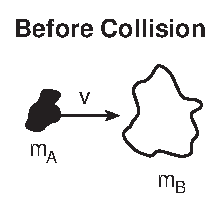
\includegraphics[keepaspectratio,scale=0.75]{June2008-Q43-left}
        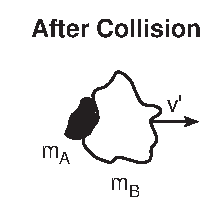
\includegraphics[keepaspectratio,scale=0.75]{June2008-Q43-right}
    \end{center}
    Which expression represents the speed, $v'$, of the masses after collision?
    Assume no outside forces are acting on $m_A$ or $m_B$.
    \begin{multicols}{2}
    \begin{choices}
        \wrongchoice{$\dfrac{m_A + m_B}{v}$}
        \wrongchoice{$\dfrac{m_A + m_B}{m_A v}$}
        \wrongchoice{$\dfrac{m_B v}{m_A + m_B}$}
      \correctchoice{$\dfrac{m_A v}{m_a + m_B}$}
    \end{choices}
    \end{multicols}
\end{question}
}


%% Section Jan2008
%%--------------------
\element{nysed}{
\begin{question}{Jan2008-Q05}
    Which object has the greatest inertia?
    \begin{choices}
        \wrongchoice{a \SI{5.00}{\kilo\gram} mass moving at \SI{10.0}{\meter\per\second}}
        \wrongchoice{a \SI{10.0}{\kilo\gram} mass moving at \SI{1.00}{\meter\per\second}}
        \wrongchoice{a \SI{15.0}{\kilo\gram} mass moving at \SI{10.0}{\meter\per\second}}
      \correctchoice{a \SI{20.0}{\kilo\gram} mass moving at \SI{1.00}{\meter\per\second}}
    \end{choices}
\end{question}
}

\element{nysed}{
\begin{question}{Jan2008-Q11}
    A \SI{6.0}{\kilo\gram} block, sliding to the east across a horizontal,
        frictionless surface with a momentum of \SI{30}{\kilo\gram\meter\per\second}, strikes an obstacle.
    The obstacle exerts an impulse of \SI{10}{\newton\second} to the west on the block.
    The speed of the block after the collision is:
    \begin{multicols}{2}
    \begin{choices}
        \wrongchoice{\SI{1.7}{\meter\per\second}}
      \correctchoice{\SI{3.3}{\meter\per\second}}
        \wrongchoice{\SI{5.0}{\meter\per\second}}
        \wrongchoice{\SI{20}{\meter\per\second}}
    \end{choices}
    \end{multicols}
\end{question}
}

\element{nysed}{
\begin{question}{Jan2008-Q13}
    A \SI{1.0}{\kilo\gram} laboratory car moving with a velocity of \SI{0.5}{\meter\per\second} due east collides with and sticks to a similar cart initially at rest.
    After the collision, the two carts move off together with a velocity of \SI{0.25}{\meter\per\second} due east.
    The total momentum of this frictionless system is:
    \begin{choices}
        \wrongchoice{zero before the collision}
        \wrongchoice{zero after the collision}
      \correctchoice{the same before and after the collision}
        \wrongchoice{greater before the collision than after the collision}
    \end{choices}
\end{question}
}


%% Section June2007
%%--------------------
\element{nysed}{
\begin{question}{June2007-Q09}
    Which situation will produce the greatest change of momentum for a \SI{1.0}{\kilo\gram} cart?
    \begin{choices}
      \correctchoice{applying a net force of \SI{5.0}{\newton} for \SI{2.0}{\second}}
        \wrongchoice{accelerating it from rest to \SI{3.0}{\meter\per\second}}
        \wrongchoice{accelerating it from \SI{2.0}{\meter\per\second} to \SI{4.0}{\meter\per\second}}
        \wrongchoice{applying a net force of \SI{10.0}{\newton} for \SI{0.5}{\second}}
    \end{choices}
\end{question}
}

\element{nysed}{
\begin{question}{June2007-Q42}
    In the diagram below, scaled vectors represent the momentum of each of two masses,
        $A$ and $B$, sliding toward each other on a frictionless, horizontal surface.
    \begin{center}
    %% NOTE: TODO: draw tikz
    \begin{tikzpicture}
        %% Block A 2cm
        \draw[thick] (-3,0) rectangle (-2,1);
        \node[anchor=center] at (-2.5,0.5) {$A$};
        \draw[thick,->] (-2,0.5) -- (0.0,0.5);
        %% Block B 0.66cm
        \draw[thick] (3,0) rectangle (2,1);
        \node[anchor=center] at (2.5,0.5) {$B$};
        \draw[thick,->] (2,0.5) -- (1.33,0.5);
        %% Floor
        \draw[thick] (-3,0) -- (3,0);
        \foreach \x in {-30,-29,...,30}
            \draw[thin] (\x mm,0cm) -- ++ (220:0.15cm);
        \node[anchor=north] at (0,-0.15) {Frictionless surface};
    \end{tikzpicture}
    \end{center}
    What scaled vector best represents the momentum of the system after the masses collide?
    [Vectors are drawn to scale]
    \begin{multicols}{2}
    \begin{choices}
        \AMCboxDimensions{down=-0.25cm}
        \correctchoice{
            \begin{tikzpicture}
                \draw[white] (-0.5,-0.5) rectangle (2,0.5);
                \draw[thick,->] (0,0) -- (1.33,0);
            \end{tikzpicture}
        }
        \wrongchoice{
            \begin{tikzpicture}
                \draw[white] (-0.5,-0.5) rectangle (2,0.5);
                \draw[thick,->] (0,0) -- (2,0);
            \end{tikzpicture}
        }
        \wrongchoice{
            \begin{tikzpicture}
                \draw[white] (-0.5,-0.5) rectangle (2,0.5);
                \draw[thick,<-] (0,0) -- (0.66,0);
            \end{tikzpicture}
        }
        \wrongchoice{
            \begin{tikzpicture}
                \draw[white] (-0.5,-0.5) rectangle (2,0.5);
                \draw[thick,<-] (0,0) -- (1.33,0);
            \end{tikzpicture}
        }
    \end{choices}
    \end{multicols}
\end{question}
}


%% Section Jan2007
%%--------------------
\element{nysed}{
\begin{question}{Jan2007-Q08}
    A woman with horizontal velocity $v_1$ jumps off a dock into a stationary boat.
    After landing in the boat,
        the woman and the boat move with velocity $v_2$.
    Compared to velocity $v_1$, velocity $v_2$ has:
    \begin{choices}
      \correctchoice{smaller magnitude and the same direction}
        \wrongchoice{larger magnitude and the same direction}
        \wrongchoice{the same magnitude and the same direction}
        \wrongchoice{the same magnitude and opposite direction}
    \end{choices}
\end{question}
}

\element{nysed}{
\begin{question}{Jan2007-Q09}
    Which object has the greatest inertia?
    \begin{choices}
        \wrongchoice{a \SI{5.0}{\kilo\gram} object moving at a speed of \SI{5.0}{\meter\per\second}}
        \wrongchoice{a \SI{10}{\kilo\gram} object moving at a speed of \SI{3.0}{\meter\per\second}}
        \wrongchoice{a \SI{15}{\kilo\gram} object moving at a speed of \SI{1.0}{\meter\per\second}}
      \correctchoice{a \SI{20}{\kilo\gram} object at rest}
    \end{choices}
\end{question}
}


%% Section June2006
%%--------------------
\element{nysed}{
\begin{question}{June2006-Q05}
    Which object has the greatest inertia?
    \begin{choices}
        \wrongchoice{a \SI{1.0}{\kilo\gram} object moving at \SI{15}{\meter\per\second}}
        \wrongchoice{a \SI{5.0}{\kilo\gram} object at rest}
        \wrongchoice{a \SI{10}{\kilo\gram} object moving at \SI{2.0}{\meter\per\second}}
      \correctchoice{a \SI{15}{\kilo\gram} object at rest}
    \end{choices}
\end{question}
}

\element{nysed}{
\begin{question}{June2006-Q40}
    A \SI{3.0}{\kilo\gram} steel block is at rest on a friction-less horizontal surface.
    A \SI{1.0}{\kilo\gram} lump of clay is propelled horizontally at \SI{6.0}{\meter\per\second} toward the block as shown in the diagram below.
    \begin{center}
        %% NOTE: TODO: priority for tikz
        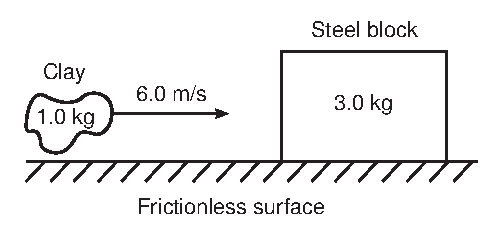
\includegraphics[keepaspectratio,scale=0.8]{June2006-Q40}
    \end{center}
    Upon collision,
        the clay and steel block stick together and move to the right with a speed of:
    \begin{multicols}{2}
    \begin{choices}
      \correctchoice{\SI{1.5}{\meter\per\second}}
        \wrongchoice{\SI{2.0}{\meter\per\second}}
        \wrongchoice{\SI{3.0}{\meter\per\second}}
        \wrongchoice{\SI{6.0}{\meter\per\second}}
    \end{choices}
    \end{multicols}
\end{question}
}


%% Section Jan2006
%%--------------------
\element{nysed}{
\begin{question}{Jan2006-Q45}
    In the diagram below, a block of mass $M$ initially at rest on a frictionless horizontal surface is struck by a bullet of mass $m$ moving with horizontal velocity $v$.
    \begin{center}
        %% NOTE: tikz would be easy
        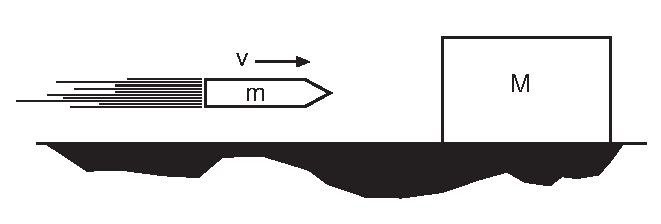
\includegraphics[keepaspectratio,scale=0.75]{Jan2006-Q45}
    \end{center}
    What is the velocity of the bullet-block system after the bullet embeds itself into the block?
    \begin{multicols}{2}
    \begin{choices}
        \wrongchoice{$\dfrac{M+v}{M}m$}
        \wrongchoice{$\dfrac{m+M}{m}v$}
        \wrongchoice{$\dfrac{m+v}{M}m$}
      \correctchoice{$\dfrac{m}{m+M}v$}
    \end{choices}
    \end{multicols}
\end{question}
}


%% Section June2005
%%--------------------
\element{nysed}{
\begin{question}{June2005-Q06}
    At the circus, a \SI{100}{\kilo\gram} clown is fired at \SI{15}{\meter\per\second} from a \SI{500}{\kilo\gram} cannon.
    What is the recoil speed of the cannon?
    \begin{multicols}{2}
    \begin{choices}
      \correctchoice{\SI{3.0}{\meter\per\second}}
        \wrongchoice{\SI{5.0}{\meter\per\second}}
        \wrongchoice{\SI{75}{\meter\per\second}}
        \wrongchoice{\SI{15}{\meter\per\second}}
    \end{choices}
    \end{multicols}
\end{question}
}

\element{nysed}{
\begin{question}{June2006-Q38}
    A force of \SI{6.0}{\newton} changes the momentum of a moving object by \SI{3.0}{\kilo\gram\meter\per\second}.
    How long did the force act on the mass?
    \begin{multicols}{2}
    \begin{choices}
      \correctchoice{\SI{0.5}{\second}}
        \wrongchoice{\SI{0.25}{\second}}
        \wrongchoice{\SI{1.0}{\second}}
        \wrongchoice{\SI{2.0}{\second}}
    \end{choices}
    \end{multicols}
\end{question}
}


%% Section Jan2005
%%--------------------
\element{nysed}{
\begin{question}{Jan2005-Q04}
    In the diagram below,
        a \SI{60}{\kilo\gram} roller-skater exerts a \SI{10}{\newton} force on a \SI{30}{\kilo\gram} roller-skater for \SI{0.20}{\second}.
    \begin{center}
        %% NOTE: cannot tikz
        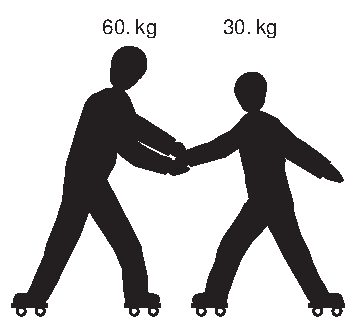
\includegraphics[keepaspectratio,scale=0.80]{Jan2005-Q04}
    \end{center}
    What is the magnitude of the impulse applied to the \SI{30}{\kilo\gram} roller-skater?
    \begin{multicols}{2}
    \begin{choices}
      \correctchoice{\SI{2.0}{\newton\second}}
        \wrongchoice{\SI{50}{\newton\second}}
        \wrongchoice{\SI{6.0}{\newton\second}}
        \wrongchoice{\SI{12}{\newton\second}}
    \end{choices}
    \end{multicols}
\end{question}
}

\element{nysed}{
\begin{question}{Jan2005-Q08}
    A lab cart is loaded with different masses and moved at various velocities.
    Which diagram shows the cart-mass system with the greatest inertia?
    \begin{multicols}{2}
    \begin{choices}
        %% NOTE: TODO: draw tikz
        \wrongchoice{
            \begin{tikzpicture}[scale=0.80]
                %% Cart
                \draw[fill=black!25!white] (-2,0.5) rectangle (2,1.5);
                \draw[thick,fill=white] (-1.0,0.5) circle (0.5cm);
                \draw[thick,fill=white] (+1.0,0.5) circle (0.5cm);
                %% Mass
                \draw (-1.0,1.5) rectangle (1,3.5);
                \draw[thick,->] (-1,4) -- (1,4)
                    node[pos=0.5,anchor=south] {\SI{4}{\meter\per\second}};
                %% Ground
                \draw[thick] (-2.5,0) -- (2.5,0);
                \foreach \x in {-25,-23,...,25}
                    \draw[thin] (\x mm,0cm) -- ++ (220:0.15cm);
                %\node[anchor=north] at (0,-0.15) {Frictionless surface};
            \end{tikzpicture}
        }
        %\wrongchoice{\includegraphics[keepaspectratio,scale=0.66]{June2005-Q08-A}}
        %\wrongchoice{\includegraphics[keepaspectratio,scale=0.66]{June2005-Q08-B}}
        %\wrongchoice{\includegraphics[keepaspectratio,scale=0.66]{June2005-Q08-C}}
        %\correctchoice{\includegraphics[keepaspectratio,scale=0.66]{June2005-Q08-D}}
    \end{choices}
    \end{multicols}
\end{question}
}


%% Section June2004
%%--------------------
\element{nysed}{
\begin{question}{June2004-Q09}
    A \SI{50}{\kilo\gram} student threw a \SI{0.40}{\kilo\gram} ball with a speed of \SI{20}{\meter\per\second}.
    What was the magnitude of the impulse that the student exerted on the ball?
    \begin{multicols}{2}
    \begin{choices}
      \correctchoice{\SI{8.0}{\newton\second}}
        \wrongchoice{\SI{78}{\newton\second}}
        \wrongchoice{\SI{4.0e2}{\newton\second}}
        \wrongchoice{\SI{1.0e3}{\newton\second}}
    \end{choices}
    \end{multicols}
\end{question}
}

%% Section Jan2004
%%--------------------
\element{nysed}{
\begin{question}{Jan2004-Q05}
    Which object has the most inertia?
    \begin{choices}
        \wrongchoice{a \SI{0.001}{\kilo\gram} bumblebee traveling at \SI{2}{\meter\per\second}}
        \wrongchoice{a \SI{0.1}{\kilo\gram} baseball traveling at \SI{20}{\meter\per\second}}
        \wrongchoice{a \SI{5}{\kilo\gram} bowling ball traveling at \SI{3}{\meter\per\second}}
      \correctchoice{a \SI{10}{\kilo\gram} sled at rest}
    \end{choices}
\end{question}
}

\element{nysed}{
\begin{question}{Jan2004-Q12}
    What is the speed of a \SI{1.0e3}{\kilo\gram} car that has a momentum of \SI{2.0e4}{\kilo\gram\meter\per\second} east?
    \begin{multicols}{2}
    \begin{choices}
      \correctchoice{\SI{2.0e1}{\meter\per\second}}
        \wrongchoice{\SI{5.0e-2}{\meter\per\second}}
        \wrongchoice{\SI{1.0e4}{\meter\per\second}}
        \wrongchoice{\SI{2.0e7}{\meter\per\second}}
    \end{choices}
    \end{multicols}
\end{question}
}


%% Section June2003
%%--------------------
\element{nysed}{
\begin{question}{June2003-Q12}
    Ball $A$ of mass \SI{5.0}{\kilo\gram} moving at \SI{20}{\meter\per\second} collides with ball $B$ of unknown mass moving at \SI{10}{\meter\per\second} in the same direction.
    After the collision,
        ball $A$ moves at \SI{10}{\meter\per\second} and ball $B$ at \SI{15}{\meter\per\second},
        both still in the same direction.
    What is the mass of ball $B$?
    \begin{multicols}{2}
    \begin{choices}
      \correctchoice{\SI{10.}{\kilo\gram}}
        \wrongchoice{\SI{6.0}{\kilo\gram}}
        \wrongchoice{\SI{12.}{\kilo\gram}}
        \wrongchoice{\SI{2.0}{\kilo\gram}}
    \end{choices}
    \end{multicols}
\end{question}
}

\element{nysed}{
\begin{question}{June2003-Q15}
    Which person has the greatest inertia?
    \begin{choices}
      \correctchoice{a \SI{110}{\kilo\gram} wrestler resting on a mat}
        \wrongchoice{a \SI{90}{\kilo\gram} man walking at \SI{2}{\meter\per\second}}
        \wrongchoice{a \SI{70}{\kilo\gram} long-distance runner traveling at \SI{5}{\meter\per\second}}
        \wrongchoice{a \SI{50}{\kilo\gram} girl sprinting at \SI{10}{\meter\per\second}}
    \end{choices}
\end{question}
}

%% Section Aug2002
%%--------------------
\element{nysed}{
\begin{question}{Aug2002-Q25}
    Which is an acceptable unit for impulse?
    \begin{choices}
        \wrongchoice{newton meter (\si{\newton\meter})}
        \wrongchoice{joule per second (\si{\joule\per\second})}
        \wrongchoice{joule second (\si{\joule\second})}
      \correctchoice{kilogram meter per second (\si{\kilo\gram\meter\second})}
    \end{choices}
\end{question}
}

\element{nysed}{
\begin{question}{Aug2002-Q36}
    The diagram below shows a \SI{4.0}{\kilo\gram} cart moving to the right and a \SI{6.0}{\kilo\gram} cart moving to the left on a horizontal frictionless surface.
    \begin{center}
    \begin{tikzpicture}
        %% Ground
        \node[anchor=north,fill,pattern=north east lines,minimum width=8cm, minimum height=0.05cm] at (0,0) {};
        \draw (-4,0) -- (4,0);
        %% left Cart
        \node[draw,minimum height=1.0cm,minimum width=1.5cm,anchor=south] (L) at (-2.5,0.2) {\SI{4.0}{\kilo\gram}};
        \draw[fill=white] (L.south west) ++(0:0.4) circle (0.2);
        \draw[fill=black] (L.south west) ++(0:0.4) circle (1pt);
        \draw[fill=white] (L.south east) ++(180:0.4) circle (0.2);
        \draw[fill=black] (L.south east) ++(180:0.4) circle (1pt);
        \draw[thick,->] (L.north west) ++(90:0.5) -- ++(0:1.5) node[pos=0.5,anchor=south] {\SI{3.0}{\meter\per\second}};
        %% right Cart
        \node[draw,minimum height=1.2cm,minimum width=1.8cm,anchor=south] (R) at (+2.5,0.2) {\SI{6.0}{\kilo\gram}};
        \draw[fill=white] (R.south west) ++(0:0.3) circle (0.2);
        \draw[fill=black] (R.south west) ++(0:0.3) circle (1pt);
        \draw[fill=white] (R.south east) ++(180:0.3) circle (0.2);
        \draw[fill=black] (R.south east) ++(180:0.3) circle (1pt);
        \draw[thick,->] (R.north east) ++(90:0.5) -- ++(180:1.5) node[pos=0.5,anchor=south] {\SI{3.0}{\meter\per\second}};
    \end{tikzpicture}
    \end{center}
    When the two carts collide they lock together.
    The magnitude of the total momentum of the two-cart system after the collision is:
    \begin{multicols}{2}
    \begin{choices}
        \wrongchoice{\SI{0.0}{\kilo\gram\meter\per\second}}
      \correctchoice{\SI{6.0}{\kilo\gram\meter\per\second}}
        \wrongchoice{\SI{15}{\kilo\gram\meter\per\second}}
        \wrongchoice{\SI{30}{\kilo\gram\meter\per\second}}
    \end{choices}
    \end{multicols}
\end{question}
}


%% Section June2002
%%--------------------
\element{nysed}{
\begin{question}{June2002-Q11}
    A \SI{0.10}{\kilo\gram} model rocket's engine is designed to deliver an impulse of \SI{6.0}{\newton\second}.
    If the rocket engine burns for \SI{0.75}{\second},
        what average force does it produce?
    \begin{multicols}{2}
    \begin{choices}
        \wrongchoice{\SI{4.5}{\newton}}
      \correctchoice{\SI{8.0}{\newton}}
        \wrongchoice{\SI{45}{\newton}}
        \wrongchoice{\SI{80}{\newton}}
    \end{choices}
    \end{multicols}
\end{question}
}


%% Section Jan2002
%%--------------------
\element{nysed}{
\begin{question}{Jan2002-Q14}
    A bullet traveling at \SI{5.0e2}{\meter\per\second} is brought to rest by an impulse of \SI{50}{\newton\second}.
    What is the mass of the bullet?
    \begin{multicols}{2}
    \begin{choices}
        \wrongchoice{\SI{1.0e-2}{\kilo\gram}}
      \correctchoice{\SI{1.0e-1}{\kilo\gram}}
        \wrongchoice{\SI{1.0e1}{\kilo\gram}}
        \wrongchoice{\SI{2.5e4}{\kilo\gram}}
    \end{choices}
    \end{multicols}
\end{question}
}

%% NOTE: This might be cool to ask what the spring constant is
%% given the amount of compression, or give two values and state the difference
\element{nysed}{
\begin{question}{Jan2002-Q17}
    The diagram below shows two carts that were initially at rest on a horizontal,
        frictionless surface being pushed apart when a compressed spring attached to one of the carts is released.
    Cart $A$ has a mass of \SI{3.0}{\kilo\gram} and cart $B$ has a mass of \SI{5.0}{\kilo\gram}.
    \begin{center}
    \begin{tikzpicture}
        %% Ground
        \node[anchor=north,fill,pattern=north east lines,minimum width=8cm, minimum height=0.05cm] at (0,0) {};
        \draw (-4,0) -- (4,0);
        %% left Cart
        \node[draw,minimum height=1.0cm,minimum width=1.5cm,anchor=south] (L) at (-1.5,0.2) {\SI{3.0}{\kilo\gram}};
        \node[anchor=south] at (L.north) {$A$};
        \draw[fill=white] (L.south west) ++(0:0.4) circle (0.2);
        \draw[fill=black] (L.south west) ++(0:0.4) circle (1pt);
        \draw[fill=white] (L.south east) ++(180:0.4) circle (0.2);
        \draw[fill=black] (L.south east) ++(180:0.4) circle (1pt);
        \draw[thick,->] (L.west) -- ++(180:1.5) node[pos=0.5,anchor=south] {\SI{0.33}{\meter\per\second}};
        %% right Cart
        \node[draw,minimum height=1.3cm,minimum width=1.95cm,anchor=south] (R) at (+1.5,0.2) {\SI{5.0}{\kilo\gram}};
        \node[anchor=south] at (R.north) {$B$};
        \draw[fill=white] (R.south west) ++(0:0.3) circle (0.2);
        \draw[fill=black] (R.south west) ++(0:0.3) circle (1pt);
        \draw[fill=white] (R.south east) ++(180:0.3) circle (0.2);
        \draw[fill=black] (R.south east) ++(180:0.3) circle (1pt);
        \draw[thick,->] (R.east) -- ++(0:1.5);
        \draw[decoration={aspect=0.2,segment length=1.5mm,amplitude=3mm,coil},decorate] (R.west) -- ++(180:1);
    \end{tikzpicture}
    \end{center}
    If the speed of cart $A$ is \SI{0.33}{\meter\per\second} after the spring is released,
        what is the approximate speed of cart $B$ after the spring is released?
    \begin{multicols}{2}
    \begin{choices}
        \wrongchoice{\SI{0.12}{\meter\per\second}}
        \wrongchoice{\SI{0.33}{\meter\per\second}}
      \correctchoice{\SI{0.20}{\meter\per\second}}
        \wrongchoice{\SI{0.55}{\meter\per\second}}
    \end{choices}
    \end{multicols}
\end{question}
}


%% Section June2001
%%--------------------
\element{nysed}{
\begin{question}{June2001-Q13}
    The magnitude of the momentum of an object is \SI{64.0}{\kilo\gram\meter\per\second}.
    If the velocity of the object is doubled,
        the magnitude of the momentum of the object will be:
    \begin{multicols}{2}
    \begin{choices}
        \wrongchoice{\SI{32.0}{\kilo\gram\meter\per\second}}
        \wrongchoice{\SI{64.0}{\kilo\gram\meter\per\second}}
      \correctchoice{\SI{128}{\kilo\gram\meter\per\second}}
        \wrongchoice{\SI{256}{\kilo\gram\meter\per\second}}
    \end{choices}
    \end{multicols}
\end{question}
}

\element{nysed}{
\begin{question}{June2001-Q15}
    Satellite $A$ has a mass of \SI{1.5e3}{\kilo\gram} and is traveling east at \SI{8.0e3}{\meter\per\second}.
    Satellite $B$ is traveling west at \SI{6.0e3}{\meter\per\second}.
    The satellites collide head-on and come to rest.
    What is the mass of satellite $B$?
    \begin{multicols}{2}
    \begin{choices}
        \wrongchoice{\SI{2.7e3}{\kilo\gram}}
      \correctchoice{\SI{2.0e3}{\kilo\gram}}
        \wrongchoice{\SI{1.5e3}{\kilo\gram}}
        \wrongchoice{\SI{1.1e3}{\kilo\gram}}
    \end{choices}
    \end{multicols}
\end{question}
}


%% Section Jan2001
%%--------------------
\element{nysed}{
\begin{question}{Jan2001-Q11}
    Two cars having different weights are traveling on a level surface at difference constant velocities.
    Within the same time interval,
        greater force will always be required to stop the car that has the greater
    \begin{multicols}{2}
    \begin{choices}
        \wrongchoice{weight}
        \wrongchoice{kinetic energy}
        \wrongchoice{velocity}
      \correctchoice{momentum}
    \end{choices}
    \end{multicols}
\end{question}
}

\element{nysed}{
\begin{question}{Jan2001-Q12}
    A \SI{0.050}{\kilo\gram} bullet is fired from a \SI{4.0}{\kilo\gram} rifle that is initially at rest.
    If the bullet leaves the rifle with momentum having a magnitude of \SI{20}{\kilo\gram\meter\per\second},
        the rifle will recoil with a momentum having a magnitude of:
    \begin{multicols}{2}
    \begin{choices}
        \wrongchoice{\SI{1600}{\kilo\gram\meter\per\second}}
        \wrongchoice{\SI{80}{\kilo\gram\meter\per\second}}
      \correctchoice{\SI{20}{\kilo\gram\meter\per\second}}
        \wrongchoice{\SI{0.25}{\kilo\gram\meter\per\second}}
    \end{choices}
    \end{multicols}
\end{question}
}


%% Section June2000
%%--------------------
\element{nysed}{
\begin{question}{June2000-Q11}
    Compared to \SI{8}{\kilo\gram} of feathers,
        \SI{6}{\kilo\gram} grams of lead has:
    \begin{choices}
      \correctchoice{less mass and less inertia.}
        \wrongchoice{less mass and more inertia.}
        \wrongchoice{more mass and less inertia.}
        \wrongchoice{more mass and more inertia.}
    \end{choices}
\end{question}
}

\element{nysed}{
\begin{question}{June2000-Q15}
    A \SI{2.0}{\kilo\gram} cart moving due east at \SI{6.0}{\meter\per\second} collides with a \SI{3.0}{\kilo\gram} cart moving due west.
    The carts stick together and come to rest after the collision.
    What was the initial speed of the \SI{3.0}{\kilo\gram} cart?
    \begin{multicols}{2}
    \begin{choices}
        \wrongchoice{\SI{1.0}{\meter\per\second}}
        \wrongchoice{\SI{6.0}{\meter\per\second}}
        \wrongchoice{\SI{9.0}{\meter\per\second}}
      \correctchoice{\SI{4.0}{\meter\per\second}}
    \end{choices}
    \end{multicols}
\end{question}
}

\element{nysed}{
\begin{question}{June2000-Q16}
    What is the momentum of a \SI{1 200}{\kilo\gram} car traveling at \SI{15}{\meter\per\second} due east?
    \begin{choices}
        \wrongchoice{\SI{80}{\kilo\gram\meter\per\second} due east}
        \wrongchoice{\SI{80}{\kilo\gram\meter\per\second} due west}
      \correctchoice{\SI{1.8e4}{\kilo\gram\meter\per\second} due east}
        \wrongchoice{\SI{1.8e4}{\kilo\gram\meter\per\second} due west}
    \end{choices}
\end{question}
}


%% Section June1999
%%--------------------
\element{nysed}{
\begin{question}{June1999-Q12}
    What is the momentum of a \SI{1.5e3}{\kilo\gram} car as it travels at \SI{30}{\meter\per\second} due east for \SI{60}{\second}?
    \begin{choices}
      \correctchoice{\SI{4.5e4}{\kilo\gram\meter\per\second} east}
        \wrongchoice{\SI{4.5e4}{\kilo\gram\meter\per\second} west}
        \wrongchoice{\SI{2.7e6}{\kilo\gram\meter} east}
        \wrongchoice{\SI{2.7e6}{\kilo\gram\meter} west}
    \end{choices}
\end{question}
}

\element{nysed}{
\begin{question}{June1999-Q14}
    A \SI{2.0e3}{\kilo\gram} car collides with a tree and is brought to rest in \SI{0.50}{\second} by an average force of \SI{6.0e4}{\newton}.
    What is the magnitude of the impulse on the car during this \SI{0.50}{\second} interval?
    \begin{multicols}{2}
    \begin{choices}
        \wrongchoice{\SI{1.0e3}{\kilo\gram\second}}
      \correctchoice{\SI{3.0e4}{\newton\second}}
        \wrongchoice{\SI{1.2e5}{\newton\per\second}}
        \wrongchoice{\SI{6.0e7}{\newton\kilo\gram\second}}
    \end{choices}
    \end{multicols}
\end{question}
}

\element{nysed}{
\begin{question}{June1998-Q15}
    The velocity-time graph below represents the motion of a \SI{3}{\kilo\gram} cart along a straight line.
    The cart starts at $t=0$ and initially moves north.
    \begin{center}
    \begin{tikzpicture}
        \begin{axis}[
            axis y line=left,
            axis x line=middle,
            axis line style={->},
            ylabel={velocity},
            y unit=\si{\meter\per\second},
            ytick={-20,-10,0,10,20},
            xlabel={time},
            x unit=\si{\second},
            xtick={0,1,2,3,4,5,6,7},
            xmin=0,xmax=7.4,
            ymin=-22,ymax=22,
            grid=major,
            width=0.8\columnwidth,
            height=0.5\columnwidth,
            very thin,
        ]
        \addplot[line width=1pt,mark=\empty] plot coordinates {(0,0) (3,20) (7,-20)};
        \end{axis}
    \end{tikzpicture}
    \end{center}
    What is the magnitude of the change in momentum of the cart between $t=0$ and $t=3$ seconds?
    \begin{multicols}{2}
    \begin{choices}
        \wrongchoice{\SI{20}{\kilo\gram\meter\per\second}}
        \wrongchoice{\SI{30}{\kilo\gram\meter\per\second}}
      \correctchoice{\SI{60}{\kilo\gram\meter\per\second}}
        \wrongchoice{\SI{80}{\kilo\gram\meter\per\second}}
    \end{choices}
    \end{multicols}
\end{question}
}

\element{nysed}{
\begin{question}{June1999-Q18}
    In the diagram below, a \SI{100}{\kilo\gram} clown is fired from a \SI{500}{\kilo\gram} cannon.
    \begin{center}
        %% NOTE: too complex to bother
        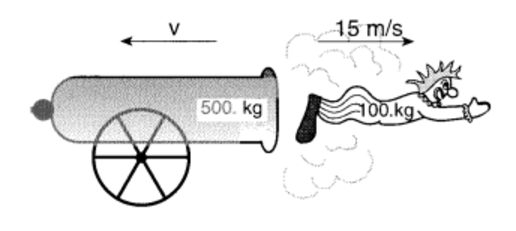
\includegraphics[keepaspectratio,scale=0.8]{June1999-Q18}
    \end{center}
    If the clown's speed is \SI{15}{\meter\per\second} after the firing,
        then the recoil speed ($v$) of the cannon is:
    \begin{multicols}{2}
    \begin{choices}
        \wrongchoice{\SI{75}{\meter\per\second}}
        \wrongchoice{\SI{15}{\meter\per\second}}
      \correctchoice{\SI{3.0}{\meter\per\second}}
        \wrongchoice{\SI{0}{\meter\per\second}}
    \end{choices}
    \end{multicols}
\end{question}
}


%% Section June1998
%%--------------------
\element{nysed}{
\begin{question}{June1998-Q51}
    During a collision between a photon and an electron,
        there is conservation of:
    \begin{choices}
        \wrongchoice{energy, only}
        \wrongchoice{momentum, only}
      \correctchoice{both energy and momentum}
        \wrongchoice{neither energy nor momentum}
    \end{choices}
\end{question}
}

\element{nysed}{
\begin{question}{June1998-Q54}
    As shown in the diagram below,
        a lump of clay travels horizontally to the right toward a block at rest on a frictionless surface.
    Upon collision, the clay and the block stick together and move to the right.
    \begin{center}
    \begin{tikzpicture}
        \begin{scope}[xshift=-2cm]
            %% Ground
            \node[anchor=north,fill,pattern=north east lines,minimum width=3.5cm, minimum height=0.05cm] at (0.25,0) {};
            \draw (-1.5,0) -- (2,0);
            %% block
            \node[draw,anchor=south,minimum size=0.75cm] (A) at (0.75,0) {};
            \node[anchor=south] at (A.north) {Block};
            %% clay
            \node[draw,circle,fill=white!60!black,minimum size=0.50cm] (B) at (-1,0.5) {};
            \node[anchor=south] at (B.north) {Clay};
            \draw[thick,->] (B.east) -- ++(0:0.5cm);
            %% label
            \node[anchor=north,yshift=-1em] at (0.25,0) {Before Collision};
        \end{scope}
        \begin{scope}[xshift=+2cm]
            %% Ground
            \node[anchor=north,fill,pattern=north east lines,minimum width=3.5cm, minimum height=0.05cm] at (0.25,0) {};
            \draw (-1.5,0) -- (2,0);
            %% clay
            \node[draw,circle,fill=white!60!black,minimum size=0.50cm] (B) at (0.5,0.5) {};
            \node[anchor=south east] at (B.north west) {Clay};
            %% block
            \node[draw,anchor=south,fill=white,minimum size=0.75cm] (A) at (1,0) {};
            \node[anchor=south] at (A.north) {Block};
            \draw[thick,->] (A.east) -- ++(0:0.5cm);
            %% label
            \node[anchor=north,yshift=-1em] at (0.25,0) {After Collision};
        \end{scope}
    \end{tikzpicture}
    \end{center}
    Compared to the total momentum of the clay and the block before the collision,
        the momentum of the clay-block system after the collisions is:
    \begin{multicols}{3}
    \begin{choices}
        \wrongchoice{less}
        \wrongchoice{greater}
      \correctchoice{the same}
    \end{choices}
    \end{multicols}
\end{question}
}


%% Section June1997
%%--------------------
\element{nysed}{
\begin{question}{June1997-Q10}
    A \SI{1000}{\kilo\gram} car traveling with a velocity of \SI[retain-explicit-plus]{+20}{\meter\per\second} decelerates at \SI{-5.0}{\meter\per\second\squared} until it comes to rest.
    What is the magnitude of the impulse applied to the car to bring it to rest?
    \begin{multicols}{2}
    \begin{choices}
        %% NOTE: kilogram meter per second?
        \wrongchoice{\SI{1.0e4}{\newton\second}}
      \correctchoice{\SI{2.0e4}{\newton\second}}
        \wrongchoice{\SI{3.9e4}{\newton\second}}
        \wrongchoice{\SI{4.3e4}{\newton\second}}
    \end{choices}
    \end{multicols}
\end{question}
}

%% NOTE: June1997-Q14 is dup of Jan2002-Q17

\element{nysed}{
\begin{question}{June1997-Q55}
    A student drops two eggs of equal mass simultaneously from the same height.
    Egg $A$ lands on the tile floor and breaks.
    Egg $B$ lands intact, without bouncing, on a foam pad lying on the floor.
    Compared to the magnitude of the impulse on egg $A$ as it lands, the magnitude of the impulse on egg $B$ as it lands is:
    \begin{multicols}{3}
    \begin{choices}
        \wrongchoice{less}
        \wrongchoice{greater}
      \correctchoice{the same}
    \end{choices}
    \end{multicols}
\end{question}
}


%% Section June1996
%%--------------------
\element{nysed}{
\begin{question}{June1996-Q17}
    A bullet traveling at \SI{5.0e2}{\meter\per\second} is brought to rest by an impulse of \SI{50}{\newton}.
    What is the mass of the bullet?
    \begin{multicols}{2}
    \begin{choices}
        \wrongchoice{\SI{2.5e4}{\kilo\gram}}
        \wrongchoice{\SI{1.0e1}{\kilo\gram}}
      \correctchoice{\SI{1.0e-1}{\kilo\gram}}
        \wrongchoice{\SI{1.0e-2}{\kilo\gram}}
    \end{choices}
    \end{multicols}
\end{question}
}

%% Section June1995
%%--------------------
\element{nysed}{
\begin{question}{June1995-Q13}
    If a net force of \SI{10}{\newton} acts on a \SI{6.0}{\kilo\gram} mass for \SI{8.0}{\second},
        the total change of momentum of the mass is:
    \begin{multicols}{2}
    \begin{choices}
        \wrongchoice{\SI{48}{\kilo\gram\meter\per\second}}
        \wrongchoice{\SI{60}{\kilo\gram\meter\per\second}}
      \correctchoice{\SI{80}{\kilo\gram\meter\per\second}}
        \wrongchoice{\SI{480}{\kilo\gram\meter\per\second}}
    \end{choices}
    \end{multicols}
\end{question}
}

\element{nysed}{
\begin{question}{June1995-Q14}
    In the diagram below, a \SI{0.4}{\kilo\gram} steel sphere and a \SI{0.1}{\kilo\gram} wooden sphere are located \SI{2.0}{\meter} above the ground.
    Both sphere are allowed to fall from rest.
    \begin{center}
    \begin{tikzpicture}
        %% ground
        \draw (-3,0) -- (3,0);
        \node[anchor=north,minimum width=6cm,pattern=north east lines] at (0,0) {};
        \node[anchor=north] at (0,-1em) {Ground};
        %% Labels
        \draw[dashed] (-3,2) -- (3,2);
        \draw[dashed] (-3,4) -- (3,4);
        \draw[latex-latex] (-2.5,0) -- (-2.5,4) node[pos=0.33,anchor=center,fill=white] {\SI{2.0}{\meter}};
        \draw[latex-latex] (-1.5,2) -- (-1.5,4) node[pos=0.5,anchor=center,fill=white] {\SI{1.0}{\meter}};
        %% Wood
        \draw[fill=black] (+2,4.15) circle (0.15cm) node[anchor=south,yshift=0.15cm] {Wood};
        %% Steel
        \draw[fill=white!90!black] (0,4.15) circle (0.15cm) node[anchor=south,yshift=0.15cm] {Steel};
    \end{tikzpicture}
    \end{center}
    Which statement best describes the spheres after they have fallen \SI{1.0}{\meter}?
    [Neglect air resistance.]
    \begin{choices}
        \wrongchoice{both spheres have the same speed and momentum}
      \correctchoice{both spheres have the same speed and the steel sphere has more momentum than the wooden sphere.}
        \wrongchoice{the steel sphere has greater speed and has less momentum than the wooden sphere.}
        \wrongchoice{the steel sphere has greater speed than the wooden sphere and both spheres have the same momentum.}
    \end{choices}
\end{question}
}


%% Section June1994
%%--------------------
\element{nysed}{
\begin{question}{June1994-Q15}
    A \SI{2.0}{\kilo\gram} toy cannon is at rest on a frictionless surface.
    A remote triggering device causes a \SI{0.005}{\kilo\gram} projectile to be fired from the cannon.
    Which equation describes this system after the cannon is fired?
    \begin{choices}
        \wrongchoice{mass of cannon + mass of projectile = 0}
        \wrongchoice{speed of cannon + speed of projectile = 0}
      \correctchoice{momentum of cannon + momentum of projectile = 0}
        \wrongchoice{velocity of cannon + velocity of projectile = 0}
    \end{choices}
\end{question}
}


%% Section June1990
%%--------------------
\element{nysed}{
\begin{question}{June1990-Q07}
    Which pair of terms are vector quantities?
    \begin{choices}
        \wrongchoice{force and mass}
        \wrongchoice{distance and displacement}
      \correctchoice{momentum and acceleration}
        \wrongchoice{speed and velocity}
    \end{choices}
\end{question}
}

\element{nysed}{
\begin{question}{June1990-Q11}
    A spring is compressed between two stationary blocks as shown in the diagram below.
    Block $A$ has mass of \SI{6.0}{\kilo\gram}.
    After the spring is released, block $A$ moves west at \SI{8.0}{\meter\per\second} and block $B$ moves east at \SI{16}{\meter\per\second}.
    \begin{center}
    \begin{tikzpicture}
        %% block A and B
        \node[draw,minimum size=1.5cm,anchor=center,text centered,text width=2em] (A) at (-2,0) {$A$ \SI{6.0}{\kilo\gram}};
        \node[draw,minimum size=1.5cm,anchor=center,text centered,text width=2em] (B) at (+2,0) {$B$};
        %% spring
        \draw[decoration={aspect=0.2,segment length=2.0mm,amplitude=2mm,coil},decorate] (A.east) -- (B.west);
    \end{tikzpicture}
    \end{center}
    What is the mass of block $B$?
    [Assume no frictional effects.]
    \begin{multicols}{2}
    \begin{choices}
        \wrongchoice{\SI{16}{\kilo\gram}}
        \wrongchoice{\SI{12}{\kilo\gram}}
      \correctchoice{\SI{3.0}{\kilo\gram}}
        \wrongchoice{\SI{6.0}{\kilo\gram}}
    \end{choices}
    \end{multicols}
\end{question}
}

\element{nysed}{
\begin{question}{June1990-Q14}
    A \SI{25}{\kilo\gram} mass travels east with a constant velocity of \SI{40}{\meter\per\second}.
    The momentum of this mass is:
    \begin{multicols}{2}
    \begin{choices}
      \correctchoice{\SI{1.0e3}{\kilo\gram\meter\per\second} east}
        \wrongchoice{\SI{9.8e3}{\kilo\gram\meter\per\second} east}
        \wrongchoice{\SI{1.0e3}{\kilo\gram\meter\per\second} west}
        \wrongchoice{\SI{9.8e3}{\kilo\gram\meter\per\second} west}
    \end{choices}
    \end{multicols}
\end{question}
}

\element{nysed}{
\begin{question}{June1990-Q16}
    A constant braking force of \SI{10}{\newton} applied for \SI{5}{\second} is used to stop a \SI{2.5}{\kilo\gram} cart traveling at \SI{20}{\meter\per\second}.
    The magnitude of the impulse applied to stop the cart is:
    \begin{multicols}{2}
    \begin{choices}
        \wrongchoice{\SI{10}{\newton\second}}
        \wrongchoice{\SI{30}{\newton\second}}
      \correctchoice{\SI{50}{\newton\second}}
        \wrongchoice{\SI{100}{\newton\second}}
    \end{choices}
    \end{multicols}
\end{question}
}


%% Section June1989
%%--------------------
\element{nysed}{
\begin{question}{June1989-Q17}
    What is the magnitude of the velocity of a \SI{25}{\kilo\gram} mass that is moving with a momentum of \SI{100}{\kilo\gram\meter\per\second}?
    \begin{multicols}{2}
    \begin{choices}
        \wrongchoice{\SI{0.25}{\meter\per\second}}
        \wrongchoice{\SI{2500}{\meter\per\second}}
        \wrongchoice{\SI{40}{\meter\per\second}}
      \correctchoice{\SI{4.0}{\meter\per\second}}
    \end{choices}
    \end{multicols}
\end{question}
}


%% Section June1986
%%--------------------
\element{nysed}{
\begin{question}{June1986-Q10}
    If the direction of the momentum of an object is west,
        the direction of the velocity of the object is:
    \begin{multicols}{2}
    \begin{choices}
        \wrongchoice{north}
        \wrongchoice{south}
        \wrongchoice{east}
      \correctchoice{west}
    \end{choices}
    \end{multicols}
\end{question}
}

\element{nysed}{
\begin{question}{June1986-Q11}
    An impulse $I$ is applied to an object.
    The change in the momentum of the object is:
    \begin{multicols}{4}
    \begin{choices}
      \correctchoice{$I$}
        \wrongchoice{$2I$}
        \wrongchoice{$\dfrac{I}{2}$}
        \wrongchoice{$4I$}
    \end{choices}
    \end{multicols}
\end{question}
}

\element{nysed}{
\begin{question}{June1986-Q12}
    An \SI{80}{\kilo\gram} skater and a \SI{60}{\kilo\gram} skater stand at rest in the center of a skating rink.
    The two skaters push each other apart.
    The \SI{60}{\kilo\gram} skater moves with a velocity of \SI{10}{\meter\per\second} east.
    What is the velocity of the \SI{80}{\kilo\gram} skater?
    [Neglect any frictional effects.]
    \begin{multicols}{2}
    \begin{choices}
        \wrongchoice{\SI{0.13}{\meter\per\second} west}
      \correctchoice{\SI{7.5}{\meter\per\second} west}
        \wrongchoice{\SI{10}{\meter\per\second} east}
        \wrongchoice{\SI{13}{\meter\per\second} east}
    \end{choices}
    \end{multicols}
\end{question}
}





\endinput



%
%% Energy Questions used on the
%% NYSED Physics Regents Examination
%%--------------------------------------------------

%% this section contains 42 problems


%% Section June2015
%%--------------------
\element{nysed}{
\begin{question}{June2015-Q15}
    A block slides across a rough, horizontal tabletop.
    As the block comes to rest,
        there is an increase in the block-tabletop system's:
    \begin{choices}
        \wrongchoice{gravitational potential energy}
        \wrongchoice{kinetic energy}
        \wrongchoice{elastic potential energy}
      \correctchoice{internal (thermal) energy}
    \end{choices}
\end{question}
}

\element{nysed}{
\begin{question}{June2015-Q45}
    A compressed spring in a toy is used to launch a \SI{5.00}{\gram} ball. 
    If the ball leaves the toy with an initial horizontal speed of \SI{5.00}{\meter\per\second},
        the minimum amount of potential energy stored in the compressed spring was:
    \begin{multicols}{2}
    \begin{choices}
        \wrongchoice{\SI{0.0125}{\joule}}
        \wrongchoice{\SI{0.0250}{\joule}}
      \correctchoice{\SI{0.0625}{\joule}}
        \wrongchoice{\SI{0.125}{\joule}}
    \end{choices}
    \end{multicols}
\end{question}
}


%% Section June2014
%%--------------------
\element{nysed}{
\begin{question}{June2014-Q31}
    A shopping cart slows as it moves along a level floor.
    Which statement describes the energies of the cart?
    \begin{choices}
      \correctchoice{the kinetic energy decreases and the gravitational potential energy decreases}
        \wrongchoice{the kinetic energy increases and the gravitational potential energy remains the same}
        \wrongchoice{the kinetic energy increases and the gravitational potential energy decreases}
        \wrongchoice{the kinetic energy decreases and the gravitational potential energy remains the same}
    \end{choices}
\end{question}
}

\element{nysed}{
\begin{question}{June2014-Q42}
    A \SI{25}{\gram} paper cup falls from rest off the edge of a tabletop \SI{0.90}{\meter} above the floor.
    If the cup has \SI{0.20}{\joule} of kinetic energy when it hits the floor,
        what is the total amount of energy converted into internal thermal energy during the cups fall?
    \begin{multicols}{2}
    \begin{choices}
      \correctchoice{\SI{0.02}{\joule}}
        \wrongchoice{\SI{2.2}{\joule}}
        \wrongchoice{\SI{0.22}{\joule}}
        \wrongchoice{\SI{2.20}{\joule}}
    \end{choices}
    \end{multicols}
\end{question}
}

\element{nysed}{
\begin{question}{June2014-Q44}
    Which graph best represents an object in equilibrium moving in a straight line?
    \begin{multicols}{2}
    \begin{choices}
        \AMCboxDimensions{down=-2.5em}
        \correctchoice{
            \begin{tikzpicture}
                \begin{axis}[
                    axis y line=left,
                    axis x line=bottom,
                    axis line style={->},
                    xlabel={time},
                    xtick=\empty,
                    ylabel={kinetic energy},
                    ytick=\empty,
                    xmin=0,xmax=11,
                    ymin=0,ymax=11,
                    width=\columnwidth,
                ]
                \addplot[line width=1pt,domain=0:10]{8};
                \end{axis}
            \end{tikzpicture}
        }
        \wrongchoice{
            \begin{tikzpicture}
                \begin{axis}[
                    axis y line=left,
                    axis x line=bottom,
                    axis line style={->},
                    xlabel={time},
                    xtick=\empty,
                    ylabel={distance},
                    ytick=\empty,
                    xmin=0,xmax=11,
                    ymin=0,ymax=11,
                    width=\columnwidth,
                ]
                \addplot[line width=1pt,domain=0:10]{0.1*x*x};
                \end{axis}
            \end{tikzpicture}
        }
        \wrongchoice{
            \begin{tikzpicture}
                \begin{axis}[
                    axis y line=left,
                    axis x line=bottom,
                    axis line style={->},
                    xlabel={time},
                    xtick=\empty,
                    ylabel={momentum},
                    ytick=\empty,
                    xmin=0,xmax=11,
                    ymin=0,ymax=11,
                    width=\columnwidth,
                ]
                \addplot[line width=1pt,domain=0:10]{x};
                \end{axis}
            \end{tikzpicture}
        }
        \wrongchoice{
            \begin{tikzpicture}
                \begin{axis}[
                    axis y line=left,
                    axis x line=bottom,
                    axis line style={->},
                    xlabel={time},
                    xtick=\empty,
                    ylabel={velocity},
                    ytick=\empty,
                    xmin=0,xmax=11,
                    ymin=0,ymax=11,
                    width=\columnwidth,
                ]
                \addplot[line width=1pt,domain=0:10]{10-x};
                \end{axis}
            \end{tikzpicture}
        }
    \end{choices}
    \end{multicols}
\end{question}
}

%% Section June2013
%%--------------------
\element{nysed}{
\begin{question}{June2013-Q21}
    In the diagram below, an ideal pendulum released from position
        $A$ swings freely to position $B$.
    \begin{center}
    \begin{tikzpicture}
        %% Ceiling
        \draw[thick] (-2,0) -- (2,0);
        \node[anchor=south,pattern=north east lines,minimum width=4cm] at (0,0) {};
        %% Pendulum
        \draw (0,0) -- (250:3cm);
        \draw[fill] (250:3cm) circle (3pt)
            node[below=1ex] {$A$};
        \draw (0,0) -- (290:3cm);
        \draw[fill] (290:3cm) circle (3pt)
            node[below=1ex] {$B$};
        \draw[dotted,->] (250:3cm) arc (250:270:3cm);
        \draw[dotted] (270:3cm) arc (270:290:3cm);
    \end{tikzpicture}
    \end{center}
    As the pendulum swings from $A$ to $B$, its total mechanical energy
    \begin{choices}
        \wrongchoice{decreases, then increases}
        \wrongchoice{increases, only}
        \wrongchoice{increases, then decreases}
      \correctchoice{remains the same}
    \end{choices}
\end{question}
}

\element{nysed}{
\begin{question}{June2013-Q45}
    Which graph best represents the relationship between the kinetic energy
        and the speed of a freely falling object?
    \begin{multicols}{2}
    \begin{choices}
        \AMCboxDimensions{down=-2.0em}
        \correctchoice{
            \begin{tikzpicture}
                \begin{axis}[
                    axis y line=left,
                    axis x line=bottom,
                    axis line style={->},
                    xlabel={speed},
                    xtick=\empty,
                    ylabel={kinetic energy},
                    ytick=\empty,
                    xmin=0,xmax=11,
                    ymin=0,ymax=11,
                    width=\columnwidth,
                    very thin,
                ]
                \addplot[line width=1pt,domain=0:10]{0.1*x*x};
                \end{axis}
            \end{tikzpicture}
        }
        \wrongchoice{
            \begin{tikzpicture}
                \begin{axis}[
                    axis y line=left,
                    axis x line=bottom,
                    axis line style={->},
                    xlabel={speed},
                    xtick=\empty,
                    ylabel={kinetic energy},
                    ytick=\empty,
                    xmin=0,xmax=11,
                    ymin=0,ymax=11,
                    width=\columnwidth,
                    very thin,
                ]
                \addplot[line width=1pt,domain=0:10]{x};
                \end{axis}
            \end{tikzpicture}
        }
        \wrongchoice{
            \begin{tikzpicture}
                \begin{axis}[
                    axis y line=left,
                    axis x line=bottom,
                    axis line style={->},
                    xlabel={speed},
                    xtick=\empty,
                    ylabel={kinetic energy},
                    ytick=\empty,
                    xmin=0,xmax=11,
                    ymin=0,ymax=11,
                    width=\columnwidth,
                    very thin,
                ]
                \addplot[line width=1pt,domain=0:10]{10-x};
                \end{axis}
            \end{tikzpicture}
        }
        \wrongchoice{
            \begin{tikzpicture}
                \begin{axis}[
                    axis y line=left,
                    axis x line=bottom,
                    axis line style={->},
                    xlabel={speed},
                    xtick=\empty,
                    ylabel={kinetic energy},
                    ytick=\empty,
                    xmin=0,xmax=11,
                    ymin=0,ymax=11,
                    width=\columnwidth,
                    very thin,
                ]
                \addplot[line width=1pt,domain=0:10]{5/x};
                \end{axis}
            \end{tikzpicture}
        }
    \end{choices}
    \end{multicols}
\end{question}
}


%% Section June2012
%%--------------------
\element{nysed}{
\begin{question}{June2012-Q14}
    A car uses its brakes to stop on a level road.
    During this process, there must be a conversion of kinetic energy into:
    \begin{choices}
        \wrongchoice{light energy}
        \wrongchoice{nuclear energy}
        \wrongchoice{gravitational potential energy}
      \correctchoice{internal energy}
    \end{choices}
\end{question}
}

\element{nysed}{
\begin{question}{June2012-Q50}
    A pendulum is made from a \SI{7.50}{\kilo\gram} mass attached to a rope connected to the ceiling of a gymnasium.
    The mass is pushed to the side until its position $A$,
        \SI{1.5}{\meter} higher than its equilibrium position.
    After it is released from rest at position $A$, the pendulum moved freely back and forth between positions $A$ and $B$,
        as shown in the diagram below.
    \begin{center}
    \begin{tikzpicture}
        %% Ceiling
        \draw (-2,0) -- (2,0);
        \node[anchor=south,fill,pattern=north east lines,minimum width=4cm] at (0,0) {};
        \node[anchor=south] at (0,1em) {Ceiling};
        %% height
        \draw[dashed] (-3,-4.33) -- (3,-4.33);
        \draw[dashed] (-3,-5) -- (3,-5);
        \draw[<->] (1,-4.33) -- (1,-5) node[pos=0.5,anchor=west] {\SI{1.5}{\meter}};
        %% pendulums
        \draw[dashed] (0,0) -- (240:5);
        \draw[thick] (0,0) -- (270:5);
        %% options
        \foreach \x/\y in {240/A,300/B}
            \draw[fill=white!90!black] (\x:5) circle (5pt) node[anchor=north west] {$\y$};
        \draw[fill=white!90!black] (270:5) circle (5pt) node[anchor=north,yshift=-5pt,text width=5em,text centered] {Equilibrium Position};
        \node[pin={120:\SI{7.5}{\kilo\gram}}] at (240:5) {};
    \end{tikzpicture}
    \end{center}
    What is the total amount of kinetic energy that the mass has as it swings freely through its equilibrium position?
    \begin{multicols}{2}
    \begin{choices}
        \wrongchoice{\SI{11}{\joule}}
        \wrongchoice{\SI{94}{\joule}}
      \correctchoice{\SI{110}{\joule}}
        \wrongchoice{\SI{920}{\joule}}
    \end{choices}
    \end{multicols}
\end{question}
}


%% Section June2011
%%--------------------
\element{nysed}{
\begin{question}{June2011-Q09}
    As a box pushes \SI{30}{\meter} across a horizontal floor by a constant horizontal force of \SI{25}{\newton},
        the kinetic energy of the box increases by \SI{300}{\joule}.
    How much total internal energy is produced during this process?
    \begin{multicols}{2}
    \begin{choices}
        \wrongchoice{\SI{150}{\joule}}
        \wrongchoice{\SI{250}{\joule}}
      \correctchoice{\SI{450}{\joule}}
        \wrongchoice{\SI{750}{\joule}}
    \end{choices}
    \end{multicols}
\end{question}
}

\element{nysed}{
\begin{question}{June2011-Q14}
    Which statement describes the kinetic energy and total mechanical energy of a block as it is pulled at constant speed up an incline?
    \begin{choices}
        \wrongchoice{Kinetic energy decreases and total mechanical energy increases}
        \wrongchoice{Kinetic energy decreases and total mechanical energy remains the same}
      \correctchoice{Kinetic energy remains the same and total mechanical energy increases}
        \wrongchoice{Kinetic energy remains the same and total mechanical energy remains the same}
    \end{choices}
\end{question}
}


%% Section June2010
%%--------------------
\element{nysed}{
\begin{question}{June2010-Q15}
    A wound spring provides the energy to propel a toy car across a level floor.
    At time $t_1$, the car is moving at speed $v_1$ across the floor and the spring is unwinding, as shown below.
    At time $t_f$, the spring has fully unwound and the car has coasted to a stop.
    \begin{center}
        %% NOTE: keep
        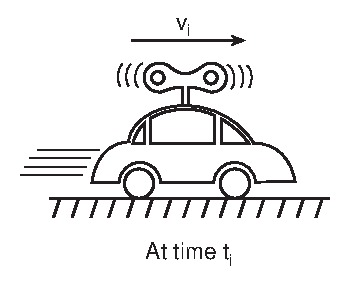
\includegraphics[keepaspectratio,scale=0.55]{June2010-Q15-left}
        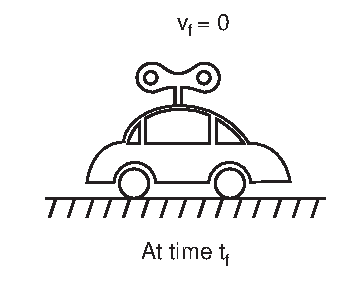
\includegraphics[keepaspectratio,scale=0.55]{June2010-Q15-right}
    \end{center}
    Which statement best describes the transformation of energy that occurs between times $t_1$ and $t_f$?
    \begin{choices}
        \wrongchoice{Gravitational potential energy at $t_1$ is converted to internal energy at $t_f$.}
        \wrongchoice{Elastic potential energy at $t_1$ is converted to kinetic energy at $t_f$.}
      \correctchoice{Both elastic potential energy and kinetic energy at $t_1$ are converted to internal energy at $t_f$.}
        \wrongchoice{Both kinetic energy and internal energy at $t_1$ are converted to elastic potential energy at $t_f$.}
    \end{choices}
\end{question}
}

\element{nysed}{
\begin{question}{June2010-Q39}
    A ball is dropped from the top of a cliff.
    Which graph best represents the relationship between the ball's total energy and elapsed time as the ball falls to the ground?
    [Neglect friction.]
    \begin{multicols}{2}
    \begin{choices}
        \AMCboxDimensions{down=-2.5em}
        \correctchoice{
            \begin{tikzpicture}
                \begin{axis}[
                    axis y line=left,
                    axis x line=bottom,
                    axis line style={->},
                    xlabel={time},
                    xtick=\empty,
                    ylabel={total energy},
                    ytick=\empty,
                    xmin=0,xmax=11,
                    ymin=0,ymax=11,
                    width=\columnwidth,
                    very thin,
                ]
                \addplot[line width=1pt,domain=0:10]{8};
                \end{axis}
            \end{tikzpicture}
        }
        \wrongchoice{
            \begin{tikzpicture}
                \begin{axis}[
                    axis y line=left,
                    axis x line=bottom,
                    axis line style={->},
                    xlabel={time},
                    xtick=\empty,
                    ylabel={total energy},
                    ytick=\empty,
                    xmin=0,xmax=11,
                    ymin=0,ymax=11,
                    width=\columnwidth,
                    very thin,
                ]
                \addplot[line width=1pt,domain=0:10]{x};
                \end{axis}
            \end{tikzpicture}
        }
        \wrongchoice{
            \begin{tikzpicture}
                \begin{axis}[
                    axis y line=left,
                    axis x line=bottom,
                    axis line style={->},
                    xlabel={time},
                    xtick=\empty,
                    ylabel={total energy},
                    ytick=\empty,
                    xmin=0,xmax=11,
                    ymin=0,ymax=11,
                    width=\columnwidth,
                    very thin,
                ]
                \addplot[line width=1pt,domain=0:10]{0.1*x*x};
                \end{axis}
            \end{tikzpicture}
        }
        \wrongchoice{
            \begin{tikzpicture}
                \begin{axis}[
                    axis y line=left,
                    axis x line=bottom,
                    axis line style={->},
                    xlabel={time},
                    xtick=\empty,
                    ylabel={total energy},
                    ytick=\empty,
                    xmin=0,xmax=11,
                    ymin=0,ymax=11,
                    width=\columnwidth,
                    very thin,
                ]
                \addplot[line width=1pt,domain=0:10]{10-x};
                \end{axis}
            \end{tikzpicture}
        }
    \end{choices}
    \end{multicols}
\end{question}
}

\element{nysed}{
\begin{question}{June2010-Q40}
    A child, starting from rest at the top of a playground slide,
        reaches a speed of \SI{7.0}{\meter\per\second} at the bottom of the slide.
    What is the vertical height of the slide?
    [Neglect friction.]
    \begin{multicols}{2}
    \begin{choices}
        \wrongchoice{\SI{0.71}{\meter}}
        \wrongchoice{\SI{1.4}{\meter}}
      \correctchoice{\SI{2.5}{\meter}}
        \wrongchoice{\SI{3.5}{\meter}}
    \end{choices}
    \end{multicols}
\end{question}
}


%% Section June2009
%%--------------------
\element{nysed}{
\begin{question}{June2009-Q15}
    As a ball falls freely toward the ground,
        its total mechanical energy:
    \begin{choices}
        \wrongchoice{decreases}
        \wrongchoice{increases}
      \correctchoice{remains the same}
    \end{choices}
\end{question}
}


%% Section Jan2009
%%--------------------
\element{nysed}{
\begin{question}{Jan2009-Q39}
    A wooden crate is pushed at constant speed across a level wooden floor.
    Which graph best represents the relationship between the total mechanical energy of the crate and the duration of time the crate is pushed?
    \begin{multicols}{2}
    \begin{choices}
        \AMCboxDimensions{down=-2.5em}
        \correctchoice{
            \begin{tikzpicture}
                \begin{axis}[
                    axis y line=left,
                    axis x line=bottom,
                    axis line style={->},
                    xlabel={time},
                    xtick=\empty,
                    ylabel={total energy},
                    ytick=\empty,
                    xmin=0,xmax=11,
                    ymin=0,ymax=11,
                    width=\columnwidth,
                    very thin,
                ]
                \addplot[line width=1pt,domain=0:10]{8};
                \end{axis}
            \end{tikzpicture}
        }
        \wrongchoice{
            \begin{tikzpicture}
                \begin{axis}[
                    axis y line=left,
                    axis x line=bottom,
                    axis line style={->},
                    xlabel={time},
                    xtick=\empty,
                    ylabel={total energy},
                    ytick=\empty,
                    xmin=0,xmax=11,
                    ymin=0,ymax=11,
                    width=\columnwidth,
                    very thin,
                ]
                \addplot[line width=1pt,domain=0:10]{0.1*x*x};
                \end{axis}
            \end{tikzpicture}
        }
        \wrongchoice{
            \begin{tikzpicture}
                \begin{axis}[
                    axis y line=left,
                    axis x line=bottom,
                    axis line style={->},
                    xlabel={time},
                    xtick=\empty,
                    ylabel={total energy},
                    ytick=\empty,
                    xmin=0,xmax=11,
                    ymin=0,ymax=11,
                    width=\columnwidth,
                    very thin,
                ]
                \addplot[line width=1pt,domain=0:10]{x};
                \end{axis}
            \end{tikzpicture}
        }
        \wrongchoice{
            \begin{tikzpicture}
                \begin{axis}[
                    axis y line=left,
                    axis x line=bottom,
                    axis line style={->},
                    xlabel={time},
                    xtick=\empty,
                    ylabel={total energy},
                    ytick=\empty,
                    xmin=0,xmax=11,
                    ymin=0,ymax=11,
                    width=\columnwidth,
                    very thin,
                ]
                \addplot[line width=1pt,domain=0:10]{10 - 0.1*(x-10)*(x-10)};
                \end{axis}
            \end{tikzpicture}
        }
    \end{choices}
    \end{multicols}
\end{question}
}

\element{nysed}{
\begin{question}{Jan2009-Q41}
    A book of mass $m$ falls freely from rest to the floor from the top of a desk of height $h$.
    what is the speed of the book upon striking the floor?
    \begin{multicols}{2}
    \begin{choices}
      \correctchoice{$\sqrt{2gh}$}
        \wrongchoice{$2gh$}
        \wrongchoice{$mgh$}
        \wrongchoice{$mh$}
    \end{choices}
    \end{multicols}
\end{question}
}


%% Section June2008
%%--------------------
\element{nysed}{
\begin{question}{June2008-Q18}
    A car travels at constant speed $v$ up a hill from point $A$ to point $B$, as shown in the diagram below.
    \begin{center}
    \begin{tikzpicture}
        %% Ground
        \draw (0,0) -- (6,0);
        \node[anchor=north,fill,pattern=north east lines,minimum width=6cm] at (3,0) {};
        \node[anchor=north] at (3,-1em) {Horizontal};
        \draw (0,0) -- (15:{6/cos(15)});
        %% points A and B
        \fill (15:1) circle (1.5pt) node[anchor=south] {$A$};
        \fill (15:6) circle (1.5pt) node[anchor=south] {$B$};
        %% car
        \path (15:3) ++(110:0.2)  node[draw,minimum height=0.5cm,minimum width=1.5cm,anchor=south,rotate=15] (C) {};
        \draw[fill=white] (C.south west) ++(15:0.4) circle (0.2);
        \draw[fill=black] (C.south west) ++(15:0.4) circle (1pt);
        \draw[fill=white] (C.south east) ++(195:0.4) circle (0.2);
        \draw[fill=black] (C.south east) ++(195:0.4) circle (1pt);
        %% velocity
        \draw[thick,->] (C.east) -- ++(15:1) node[pos=0.5,anchor=south,rotate=15] {$v$};
    \end{tikzpicture}
    \end{center}
    As the car travels from $A$ to $B$, its gravitational potential energy:
    \begin{choices}
        \wrongchoice{increases and its kinetic energy decreases}
      \correctchoice{increases and its kinetic energy remains the same}
        \wrongchoice{remains the same and its kinetic energy decreases}
        \wrongchoice{remains the same and its kinetic remains the same}
    \end{choices}
\end{question}
}

\element{nysed}{
\begin{question}{June2008-Q45}
    An object is thrown vertically upward, which pair of graphs best represents the object's kinetic energy and gravitational potential energy as functions of its displacement while it rises?
    \begin{choices}
        \AMCboxDimensions{down=-2.5em}
        \correctchoice{
            \begin{tikzpicture}
                \begin{groupplot}[
                        axis y line=left,
                        axis x line=bottom,
                        axis line style={->},
                        group style={group size=2 by 1},
                        xlabel={displacement},
                        xtick=\empty,
                        ytick=\empty,
                        xmin=0,xmax=11,
                        ymin=0,ymax=11,
                        width=0.5\columnwidth,
                    ]
                    \nextgroupplot[
                        ylabel={kinetic energy},
                    ] \addplot[line width=1pt,domain=0:10] {10-x};
                    \nextgroupplot[
                        ylabel={potential energy},
                    ] \addplot[line width=1pt,domain=0:10] {x};
                \end{groupplot}
            \end{tikzpicture}
        }
        \wrongchoice{
            \begin{tikzpicture}
                \begin{groupplot}[
                        axis y line=left,
                        axis x line=bottom,
                        axis line style={->},
                        group style={group size=2 by 1},
                        xlabel={displacement},
                        xtick=\empty,
                        ytick=\empty,
                        xmin=0,xmax=11,
                        ymin=0,ymax=11,
                        width=0.5\columnwidth,
                    ]
                    \nextgroupplot[
                        ylabel={kinetic energy},
                    ] \addplot[line width=1pt,domain=0:10] {x};
                    \nextgroupplot[
                        ylabel={potential energy},
                    ] \addplot[line width=1pt,domain=0:10] {x};
                \end{groupplot}
            \end{tikzpicture}
        }
        \wrongchoice{
            \begin{tikzpicture}
                \begin{groupplot}[
                        axis y line=left,
                        axis x line=bottom,
                        axis line style={->},
                        group style={group size=2 by 1},
                        xlabel={displacement},
                        xtick=\empty,
                        ytick=\empty,
                        xmin=0,xmax=11,
                        ymin=0,ymax=11,
                        width=0.5\columnwidth,
                    ]
                    \nextgroupplot[
                        ylabel={kinetic energy},
                    ] \addplot[line width=1pt,domain=0:10] {8};
                    \nextgroupplot[
                        ylabel={potential energy},
                    ] \addplot[line width=1pt,domain=0:10] {10-x};
                \end{groupplot}
            \end{tikzpicture}
        }
        \wrongchoice{
            \begin{tikzpicture}
                \begin{groupplot}[
                        axis y line=left,
                        axis x line=bottom,
                        axis line style={->},
                        group style={group size=2 by 1},
                        xlabel={displacement},
                        xtick=\empty,
                        ytick=\empty,
                        xmin=0,xmax=11,
                        ymin=0,ymax=11,
                        width=0.5\columnwidth,
                    ]
                    \nextgroupplot[
                        ylabel={kinetic energy},
                    ] \addplot[line width=1pt,domain=0:10] {10-x};
                    \nextgroupplot[
                        ylabel={potential energy},
                    ] \addplot[line width=1pt,domain=0:10] {8};
                \end{groupplot}
            \end{tikzpicture}
        }
    \end{choices}
\end{question}
}


%% Section Jan2008
%%--------------------
\element{nysed}{
\begin{question}{Jan2008-Q42}
    A car with mass $m$ possesses momentum of magnitude $p$.
    Which expression correctly represents the kinetic energy, $KE$,
        of the car in terms of $m$ and $p$?
    \begin{multicols}{2}
    \begin{choices}
        \wrongchoice{$KE = \dfrac{p}{2m}$}
        \wrongchoice{$KE = \dfrac{mp^2}{2}$}
        \wrongchoice{$KE = \dfrac{mp}{2}$}
      \correctchoice{$KE = \dfrac{p^2}{2m}$}
    \end{choices}
    \end{multicols}
\end{question}
}


%% Section June2007
%%--------------------
\element{nysed}{
\begin{question}{June2007-Q12}
    A horizontal force of \SI{5.0}{\newton} acts on a \SI{3.0}{\kilo\gram} mass over a distance of \SI{6.0}{\meter} along a horizontal,
        frictionless surface.
    What is the change in kinetic energy of the mass during its movement over the \SI{6.0}{\meter} distance?
    \begin{multicols}{2}
    \begin{choices}
      \correctchoice{\SI{30}{\joule}}
        \wrongchoice{\SI{90}{\joule}}
        \wrongchoice{\SI{6.0}{\joule}}
        \wrongchoice{\SI{15}{\joule}}
    \end{choices}
    \end{multicols}
\end{question}
}


%% Section Jan2007
%%--------------------
\element{nysed}{
\begin{question}{Jan2007-Q44}
    A \SI{1.00}{\kilo\gram} ball is dropped from the top of a building.
    Just before striking the ground, the ball's speed is \SI{12.0}{\meter\per\second}.
    What was the ball's gravitational potential energy,
        relative to the ground, at the instant it was dropped?
    [Neglect friction.]
    \begin{multicols}{2}
    \begin{choices}
      \correctchoice{\SI{72.0}{\joule}}
        \wrongchoice{\SI{144}{\joule}}
        \wrongchoice{\SI{6.00}{\joule}}
        \wrongchoice{\SI{24.0}{\joule}}
    \end{choices}
    \end{multicols}
\end{question}
}


%% Section June2006
%%--------------------
\element{nysed}{
\begin{question}{June2006-Q14}
    The potential energy storied in a compressed spring is to the change in the spring's length as the kinetic energy of a moving body is to the body's
    \begin{multicols}{2}
    \begin{choices}
      \correctchoice{speed}
        \wrongchoice{mass}
        \wrongchoice{radius}
        \wrongchoice{acceleration}
    \end{choices}
    \end{multicols}
\end{question}
}

\element{nysed}{
\begin{question}{June2006-Q15}
    The diagram below shows an ideal simple pendulum.
    \begin{center}
    \begin{tikzpicture}
        \draw (-2,0) -- (2,0);
        \node[anchor=south,fill,pattern=north east lines,minimum width=4cm, minimum height=0.05cm] at (0,0) {};
        %\foreach \x in {-20,-18,...,20}
        %    \draw[thin] (\x mm,0) -- ++ (40:0.15cm);
        %% Pendulums
        %\node[fill=white,draw,circle,minimum size=8pt] (B) at (240:3cm) {};
        \node[fill=white,draw,circle,fill=white!90!black,minimum size=8pt] (B) at (225:3cm) {};
        \node[fill=white,draw,circle,fill=white!90!black,minimum size=8pt] (A) at (270:3cm) {};
        %% Draw string
        \draw (0,0) -- (B);
        \draw (0,0) -- (A);
        \draw[thick,->] (265:3cm) arc (265:230:3cm);
        %% Labels
        \node[below=1em] at (A) {$A$};
        \node[below=1em] at (B) {$B$};
    \end{tikzpicture}
    \end{center}
    As the pendulum swings from position $A$ to position $B$,
        what happens to its total mechanical energy?
    [Neglect friction.]
    \begin{choices}
      \correctchoice{It remains the same}
        \wrongchoice{It decreases}
        \wrongchoice{It increases}
    \end{choices}
\end{question}
}


%% Section Jan2006
%%--------------------
\element{nysed}{
\begin{question}{Jan2006-Q19}
    A \SI{55.0}{\kilo\gram} diver falls freely from a diving platform that is \SI{3.00}{\meter} above the surface of the water in a pool.
    When she is \SI{1.00}{\meter} above the water,
        what are her gravitational potential energy and kinetic energy with respect to the water's surface?
    %% total energy 1617 J
    \begin{choices}
      \correctchoice{$PE=\SI{540}{\joule}$ and $KE=\SI{1080}{\joule}$}
        \wrongchoice{$PE=\SI{810}{\joule}$ and $KE=\SI{810}{\joule}$}
        \wrongchoice{$PE=\SI{1620}{\joule}$ and $KE=\SI{0}{\joule}$}
        \wrongchoice{$PE=\SI{1080}{\joule}$ and $KE=\SI{540}{\joule}$}
    \end{choices}
\end{question}
}


%% Section June2005
%%--------------------
\element{nysed}{
\begin{question}{June2005-Q39}
    When a \SI{1.53}{\kilo\gram} mass is placed on a spring with a spring constant of \SI{30.0}{\newton\per\meter},
        the spring is compressed \SI{0.500}{\meter}.
    How much energy is stored in the spring?
    \begin{multicols}{2}
    \begin{choices}
      \correctchoice{\SI{3.75}{\joule}}
        \wrongchoice{\SI{7.50}{\joule}}
        \wrongchoice{\SI{15.0}{\joule}}
        \wrongchoice{\SI{30.0}{\joule}}
    \end{choices}
    \end{multicols}
\end{question}
}


%% Section Jan2005
%%--------------------
\element{nysed}{
\begin{question}{Jan2005-Q05}
    In the diagram below, a \SI{10}{\kilo\gram} block is at rest on a plane inclined at \ang{15} to the horizontal.
    \begin{center}
    \begin{tikzpicture}
        %% 15 degree incline
        \draw (0,0) --  (15:5) -- ++(270:1.29) --cycle;
        \draw[<->] (2,0) arc (0:15:2) node[pos=0.5,anchor=west] {\ang{15}};
        %% 1.0 kg block
        \node[draw,anchor=south,minimum size=1.2cm,rotate=15,fill=white!90!black] at (15:4) {\SI{1.0}{\kilo\gram}};
    \end{tikzpicture}
    \end{center}
    As the angle of the incline is increased to \ang{30},
        the mass of the block will:
    \begin{choices}
      \correctchoice{remain the same}
        \wrongchoice{decrease}
        \wrongchoice{increase}
    \end{choices}
\end{question}
}

\element{nysed}{
\begin{question}{Jan2005-Q06}
    If the direction of a moving car changes and its speed remains constant,
        which quantity must remain the same?
    \begin{multicols}{2}
    \begin{choices}
        \wrongchoice{velocity}
        \wrongchoice{displacement}
        \wrongchoice{momentum}
      \correctchoice{kinetic energy}
    \end{choices}
    \end{multicols}
\end{question}
}

\element{nysed}{
\begin{question}{Jan2005-Q46}
    As shown in the diagram below, a \SI{0.5}{\meter} long spring is stretched from its equilibrium position to a length of \SI{1.00}{\meter} by a weight.
    \begin{center}
    \begin{tikzpicture}
        \begin{scope}[xshift=-2cm]
            %% Title
            \node[anchor=south,text centered] at (0.5,0.2cm) {Unstretched};
            %% Celiing
            \draw (-1,0) --  (2,0);
            \node[anchor=south,fill,pattern=north east lines,minimum width=3cm, minimum height=0.05cm] at (0.5,0) {};
            %% Spring
            \draw[thick,decoration={aspect=0.2,segment length=1.5mm,amplitude=4mm,coil},decorate] (0,0) -- (0,-1.5);
            \draw[dashed]  (0,-1.5) -- ++(0:1cm);
            %% Ruler
            \draw[<->] (1.5,0) -- (1.5,-1.5) node[pos=0.5,anchor=center,fill=white] {\SI{0.50}{\meter}};
        \end{scope}
        \begin{scope}[xshift=+2cm]
            %% Title
            \node[anchor=south,text centered] at (0.5,0.2cm) {Stretched};
            %% Celiing
            \draw (-1,0) --  (2,0);
            \node[anchor=south,fill,pattern=north east lines,minimum width=3cm, minimum height=0.05cm] at (0.5,0) {};
            %% Weight
            \node[anchor=north,draw,minimum size=1cm] (M) at (0,-3) {Weight};
            %% Spring
            \draw[thick,decoration={aspect=0.2,segment length=3mm,amplitude=4mm,coil},decorate] (0,0) -- (0,-3);
            \draw[dashed]  (0,-3) -- ++(0:1cm);
            %% Ruler
            \draw[<->] (1.5,0) -- (1.5,-3) node[pos=0.5,anchor=center,fill=white] {\SI{1.00}{\meter}};
        \end{scope}
    \end{tikzpicture}
    \end{center}
    If \SI{15}{\joule} of energy are stored in the stretched spring,
        what is the value of the spring constant?
    \begin{multicols}{2}
    \begin{choices}
      \correctchoice{\SI{120}{\newton\per\meter}}
        \wrongchoice{\SI{240}{\newton\per\meter}}
        \wrongchoice{\SI{30}{\newton\per\meter}}
        \wrongchoice{\SI{60}{\newton\per\meter}}
    \end{choices}
    \end{multicols}
\end{question}
}


%% Section June2004
%%--------------------
\element{nysed}{
\begin{question}{June2004-Q14}
    A \SI{5}{\newton} force causes a spring to stretch \SI{0.2}{\meter}.
    What is the potential energy stored in the stretched spring?
    \begin{multicols}{2}
    \begin{choices}
      \correctchoice{\SI{0.5}{\joule}}
        \wrongchoice{\SI{1.}{\joule}}
        \wrongchoice{\SI{0.2}{\joule}}
        \wrongchoice{\SI{0.1}{\joule}}
    \end{choices}
    \end{multicols}
\end{question}
}

\element{nysed}{
\begin{question}{June2004-Q37}
    The graph below represents the kinetic energy (KE),
        gravitational potential energy (PE),
        and the total mechanical energy (TME) of a moving block.
    \begin{center}
    \begin{tikzpicture}
        \begin{axis}[
            clip=false,
            axis y line=left,
            axis x line=bottom,
            axis line style={->},
            xlabel={distance moved},
            xtick=\empty,
            ylabel={energy},
            ytick=\empty,
            xmin=0,xmax=10,
            ymin=0,ymax=11,
            width=0.98\columnwidth,
            height=0.618\columnwidth,
            very thin,
            legend style={
                at={(0.95,0.5)},
                anchor=center,
            },
        ]
        \addplot[thick,dotted,domain=0:10]{10-x};
        \addplot[thick,dashed,domain=0:10]{x};
        \addplot[thick,black,domain=0:10]{10};
        \legend{KE,PE,TME};
        \end{axis}
    \end{tikzpicture}
    \end{center}
    Which best describes the motion of the block?
    \begin{choices}
      \correctchoice{falling freely}
        \wrongchoice{being lifted at constant velocity}
        \wrongchoice{acceleration on a flat horizontal surface}
        \wrongchoice{sliding up a frictionless incline}
    \end{choices}
\end{question}
}


%% Section Jan2004
%%--------------------
\element{nysed}{
\begin{question}{Jan2004-Q14}
    If the speed of a car is doubled, the kinetic energy of the car is:
    \begin{multicols}{2}
    \begin{choices}
      \correctchoice{quadrupled}
        \wrongchoice{quartered}
        \wrongchoice{doubled}
        \wrongchoice{halved}
    \end{choices}
    \end{multicols}
\end{question}
}

\element{nysed}{
\begin{question}{Jan2004-Q16}
    The diagram below shows a \SI{0.1}{\kilo\gram} apple attached to a branch of a tree \SI{2}{\meter} above a spring on the ground below.
    \begin{center}
        %% NOTE: keep graphic
        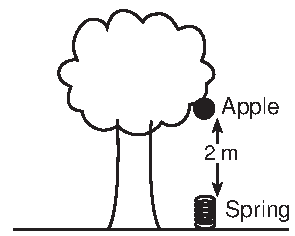
\includegraphics[keepaspectratio]{Jan2004-Q16}
    \end{center}
    The apple falls and hits the spring compressing it \SI{0.1}{\meter} from its rest position.
    If all of the gravitational potential energy of the apple on the tree is transferred to the spring when it is compressed,
        what is the spring constant of the spring?
    \begin{multicols}{2}
    \begin{choices}
      \correctchoice{\SI{400}{\newton\per\meter}}
        \wrongchoice{\SI{10}{\newton\per\meter}}
        \wrongchoice{\SI{100}{\newton\per\meter}}
        \wrongchoice{\SI{40}{\newton\per\meter}}
    \end{choices}
    \end{multicols}
\end{question}
}

\element{nysed}{
\begin{question}{Jan2004-Q17}
    A \SI{1}{\kilo\gram} rock is dropped from a cliff \SI{90}{\meter} high.
    After falling \SI{20}{\meter},
        the kinetic energy of the rock is approximately:
    \begin{multicols}{2}
    \begin{choices}
      \correctchoice{\SI{200}{\joule}}
        \wrongchoice{\SI{20}{\joule}}
        \wrongchoice{\SI{700}{\joule}}
        \wrongchoice{\SI{900}{\joule}}
    \end{choices}
    \end{multicols}
\end{question}
}


%% Section June2003
%%--------------------
\element{nysed}{
\begin{question}{June2003-Q18}
    As a ball falls freely (without friction) toward the ground,
        its total mechanical energy:
    \begin{choices}
      \correctchoice{remains the same}
        \wrongchoice{decreases}
        \wrongchoice{increases}
    \end{choices}
\end{question}
}

\element{nysed}{
\begin{question}{June2003-Q19}
    A \SI{0.50}{\kilo\gram} ball is thrown vertically upward with an initial kinetic energy of \SI{25}{\joule}.
    Approximately how high will the ball rise?
    [Neglect air resistance.]
    \begin{multicols}{2}
    \begin{choices}
      \correctchoice{\SI{5.1}{\meter}}
        \wrongchoice{\SI{2.6}{\meter}}
        \wrongchoice{\SI{13}{\meter}}
        \wrongchoice{\SI{25}{\meter}}
    \end{choices}
    \end{multicols}
\end{question}
}

\element{nysed}{
\begin{question}{June2003-Q42}
    Which graph best represents the relationship between kinetic energy and the velocity of an object accelerating in a straight line?
    \begin{multicols}{2}
    \begin{choices}
        \AMCboxDimensions{down=-2.5em}
        \correctchoice{
            \begin{tikzpicture}
                \begin{axis}[
                    axis y line=left,
                    axis x line=bottom,
                    axis line style={->},
                    xlabel={velocity},
                    xtick=\empty,
                    ylabel={kinetic energy},
                    ytick=\empty,
                    xmin=0,xmax=11,
                    ymin=0,ymax=11,
                    width=\columnwidth,
                    very thin,
                ]
                \addplot[line width=1pt,domain=0:10]{7};
                \end{axis}
            \end{tikzpicture}
        }
        \wrongchoice{
            \begin{tikzpicture}
                \begin{axis}[
                    axis y line=left,
                    axis x line=bottom,
                    axis line style={->},
                    xlabel={velocity},
                    xtick=\empty,
                    ylabel={kinetic energy},
                    ytick=\empty,
                    xmin=0,xmax=11,
                    ymin=0,ymax=11,
                    width=\columnwidth,
                    very thin,
                ]
                \addplot[line width=1pt,domain=0:10]{x};
                \end{axis}
            \end{tikzpicture}
        }
        \wrongchoice{
            \begin{tikzpicture}
                \begin{axis}[
                    axis y line=left,
                    axis x line=bottom,
                    axis line style={->},
                    xlabel={velocity},
                    xtick=\empty,
                    ylabel={kinetic energy},
                    ytick=\empty,
                    xmin=0,xmax=11,
                    ymin=0,ymax=11,
                    width=\columnwidth,
                    very thin,
                ]
                \addplot[line width=1pt,domain=0:10]{5/x};
                \end{axis}
            \end{tikzpicture}
        }
        \wrongchoice{
            \begin{tikzpicture}
                \begin{axis}[
                    axis y line=left,
                    axis x line=bottom,
                    axis line style={->},
                    xlabel={velocity},
                    xtick=\empty,
                    ylabel={kinetic energy},
                    ytick=\empty,
                    xmin=0,xmax=11,
                    ymin=0,ymax=11,
                    width=\columnwidth,
                    very thin,
                ]
                \addplot[line width=1pt,domain=0:10]{0.1*x*x};
                \end{axis}
            \end{tikzpicture}
        }
    \end{choices}
    \end{multicols}
\end{question}
}


%% Section Jan2003
%%--------------------
\element{nysed}{
\begin{question}{Jan2003-Q16}
    As an object falls freely,
        the kinetic energy of the object:
    \begin{choices}
      \correctchoice{increases}
        \wrongchoice{decreases}
        \wrongchoice{remains the same}
    \end{choices}
\end{question}
}

\element{nysed}{
\begin{question}{Jan2003-Q39}
    A constant force is used to keep a block sliding at constant velocity along a rough horizontal track.
    As the block slides, there could be an increase in its:
    \begin{choices}
      \correctchoice{internal energy, only}
        \wrongchoice{gravitational potential energy, only}
        \wrongchoice{gravitational potential energy and kinetic energy}
        \wrongchoice{internal energy and kinetic energy}
    \end{choices}
\end{question}
}


%% Section June2002
%%--------------------
\element{nysed}{
\begin{question}{Jan2002-Q16}
    What is an essential characteristic of an object in equilibrium?
    \begin{choices}
        \wrongchoice{zero velocity}
      \correctchoice{zero acceleration}
        \wrongchoice{zero potential energy}
        \wrongchoice{zero kinetic energy}
    \end{choices}
\end{question}
}

\element{nysed}{
\begin{question}{June2002-Q43}
    Which graph best represents the relationship between the gravitational potential energy of a freely falling object and the object's height above the ground near the surface of Earth.
    \begin{multicols}{2}
    \begin{choices}
        \AMCboxDimensions{down=-2.5em}
        \wrongchoice{
            \begin{tikzpicture}
                \begin{axis}[
                    axis y line=left,
                    axis x line=bottom,
                    axis line style={->},
                    xlabel={height},
                    xtick=\empty,
                    ylabel={energy},
                    ytick=\empty,
                    xmin=0,xmax=11,
                    ymin=0,ymax=11,
                    width=\columnwidth,
                    very thin,
                ]
                \addplot[line width=1pt,domain=0:10]{x};
                \end{axis}
            \end{tikzpicture}
        }
        \correctchoice{
            \begin{tikzpicture}
                \begin{axis}[
                    axis y line=left,
                    axis x line=bottom,
                    axis line style={->},
                    xlabel={height},
                    xtick=\empty,
                    ylabel={energy},
                    ytick=\empty,
                    xmin=0,xmax=11,
                    ymin=0,ymax=11,
                    width=\columnwidth,
                    very thin,
                ]
                \addplot[line width=1pt,domain=0:10]{10-x};
                \end{axis}
            \end{tikzpicture}
        }
        \wrongchoice{
            \begin{tikzpicture}
                \begin{axis}[
                    axis y line=left,
                    axis x line=bottom,
                    axis line style={->},
                    xlabel={height},
                    xtick=\empty,
                    ylabel={energy},
                    ytick=\empty,
                    xmin=0,xmax=11,
                    ymin=0,ymax=11,
                    width=\columnwidth,
                    very thin,
                ]
                \addplot[line width=1pt,domain=0:10]{8};
                \end{axis}
            \end{tikzpicture}
        }
        \wrongchoice{
            \begin{tikzpicture}
                \begin{axis}[
                    axis y line=left,
                    axis x line=bottom,
                    axis line style={->},
                    xlabel={height},
                    xtick=\empty,
                    ylabel={energy},
                    ytick=\empty,
                    xmin=0,xmax=11,
                    ymin=0,ymax=11,
                    width=\columnwidth,
                    very thin,
                ]
                \addplot[line width=1pt,domain=0:10]{0.1*x*x};
                \end{axis}
            \end{tikzpicture}
        }
    \end{choices}
    \end{multicols}
\end{question}
}


%% Section June1998
%%--------------------
\element{nysed}{
\begin{question}{June1998-Q19}
    The diagram below shows a \SI{1.5}{\kilo\gram} kitten jumping from the top of a \SI{1.80}{\meter} high refrigerator to a \SI{0.90}{\meter} high counter.
    \begin{center}
        %% NOTE: keep graphic
        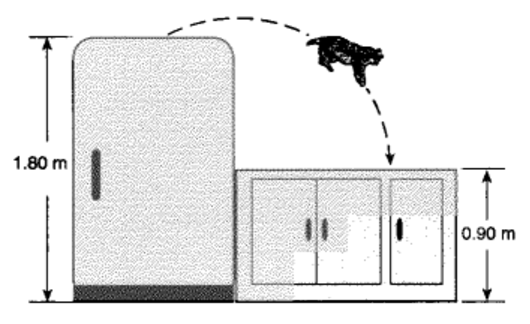
\includegraphics[keepaspectratio,scale=0.95]{June1998-Q19}
    \end{center}
    Compared to the kitten's gravitational potential energy on top of the refrigerator,
        the kitten's gravitational potential energy on top of the counter is:
    \begin{choices}
      \correctchoice{half as great}
        \wrongchoice{twice as great}
        \wrongchoice{one-fourth as great}
        \wrongchoice{four times as great}
    \end{choices}
\end{question}
}


%% Section June1997
%%--------------------


%% Section June1994
%%--------------------
\element{nysed}{
\begin{question}{June1994-Q22}
    In the diagram below, an ideal pendulum released from point $A$ swings freely through point $B$.
    \begin{center}
    \begin{tikzpicture}
        %% strings
        \draw[thick] (0,0) -- (300:4);
        \draw[dashed] (0,0) -- (270:4);
        \draw[dashed] (0,0) -- (240:4);
        %% path
        \draw[dashed] (300:4) arc (300:240:4);
        \draw[thick,->] (300:4) arc (300:285:4);
        \draw[thick,->] (270:4) arc (270:255:4);
        %% options
        \foreach \x/\y in {300/A,270/B,240/} {
            \draw[very thick,fill=white] (\x:4) circle (1ex);
            \node[anchor=center,shift={(\x:1em)}] at (\x:4) {$\y$};
        }
    \end{tikzpicture}
    \end{center}
    Compared to the pendulum's kinetic energy at $A$,
        its potential energy at $B$ is:
    \begin{multicols}{2}
    \begin{choices}
        \wrongchoice{half as great}
        \wrongchoice{twice as great}
      \correctchoice{the same}
        \wrongchoice{four times as great}
    \end{choices}
    \end{multicols}
\end{question}
}



\endinput



%
%% Work and Energy Questions used on the
%% NYSED Physics Regents Examination
%%--------------------------------------------------

%% this section contains 109 problems


%% Section June2016
%%--------------------
\element{nysed}{
\begin{question}{June2016-Q12}
    A horizontal force of \SI{20}{\newton} eastward causes a \SI{10}{\kilo\gram} box to have a displacement of \SI{5}{\meter} eastward. 
    The total work done on the box by the \SI{20}{\newton} force is:
    \begin{multicols}{2}
    \begin{choices}
        \wrongchoice{\SI{40}{\joule}}
      \correctchoice{\SI{100}{\joule}}
        \wrongchoice{\SI{200}{\joule}}
        \wrongchoice{\SI{1000}{\joule}}
    \end{choices}
    \end{multicols}
\end{question}
}

\element{nysed}{
\begin{question}{June2016-Q13}
    A block initially at rest on a horizontal,
        frictionless surface is accelerated by a constant horizontal force of \SI{5.0}{\newton}.
    If \SI{15}{\joule} of work is done on the block by this force while accelerating it,
        the kinetic energy of the block increases by:
    \begin{multicols}{2}
    \begin{choices}
        \wrongchoice{\SI{3.0}{\joule}}
      \correctchoice{\SI{15}{\joule}}
        \wrongchoice{\SI{20.}{\joule}}
        \wrongchoice{\SI{75}{\joule}}
    \end{choices}
    \end{multicols}
\end{question}
}

\element{nysed}{
\begin{question}{June2016-Q14}
    Two objects, $A$ and $B$, are held one meter above the horizontal ground. 
    The mass of $B$ is twice as great as the mass of $A$. 
    If $PE$ is the gravitational potential energy of $A$ relative to the ground,
        then the gravitational potential energy of $B$ relative to the ground is:
    \begin{multicols}{2}
    \begin{choices}
        \wrongchoice{$PE$}
      \correctchoice{$2PE$}
        \wrongchoice{$\dfrac{PE}{2}$}
        \wrongchoice{$4PE$}
    \end{choices}
    \end{multicols}
\end{question}
}

\element{nysed}{
\begin{question}{June2016-Q15}
    What is the kinetic energy of a \SI{55}{\kilogram} skier traveling at \SI{9.0}{\meter\per\second}?
    \begin{multicols}{2}
    \begin{choices}
        \wrongchoice{\SI{2.5e2}{\joule}}
        \wrongchoice{\SI{5.0e2}{\joule}}
      \correctchoice{\SI{2.2e3}{\joule}}
        \wrongchoice{\SI{4.9e3}{\joule}}
    \end{choices}
    \end{multicols}
\end{question}
}


%% Section June2015
%%--------------------
\element{nysed}{
\begin{question}{June2015-Q42}
    Which combination of fundamental units can be used to express the amount of work done on an object?
    \begin{choices}
        \wrongchoice{kilogram meter per second (\si{\kilo\gram\meter\per\second})}
        \wrongchoice{kilogram meter per second squared (\si{\kilo\gram\meter\per\second\squared})}
      \correctchoice{kilogram meter squared per second squared (\si{\kilo\gram\meter\squared\per\second\squared})}
        \wrongchoice{kilogram meter squared per second cubed (\si{\kilo\gram\meter\squared\per\second\cubed})}
    \end{choices}
\end{question}
}

\element{nysed}{
\begin{question}{June2015-Q48}
    The graph below represents the relationship between the force exerted on an elevator and the distance the elevator is lifted.
    \begin{center}
    \begin{tikzpicture}
        \begin{axis}[
            axis y line=left, 
            axis x line=bottom, 
            axis line style={->},
            xlabel={Distance Lifted},
            x unit=\si{\meter},
            xtick={0,3,6,9},
            xticklabels={$0.0$,$3.0$,$6.0$,$9.0$},
            ylabel={Force Exerted},
            y unit=\SI{e4}{\newton},
            ytick={0,1,2},
            yticklabels={$0.0$,$1.0$,$2.0$},
            xmin=0,xmax=10,
            ymin=0,ymax=2.5,
            width=0.8\columnwidth,
            height=0.5\columnwidth,
            font=\small,
        ]
        \addplot[line width=1pt,domain=0:3]{1.0};
        \addplot[line width=1pt,domain=3:10]{2.0};
        \addplot[dashed] coordinates { (3,1.0) (3,2.0) }; 
        \end{axis}
    \end{tikzpicture}
    \end{center}
    How much total work is done by the force in lifting the elevator from \SI{0.0}{\meter} to \SI{9.0}{\meter}?
    \begin{multicols}{2}
    \begin{choices}
        \wrongchoice{\SI{9.0e4}{\joule}}
        \wrongchoice{\SI{1.2e5}{\joule}}
      \correctchoice{\SI{1.5e5}{\joule}}
        \wrongchoice{\SI{1.8e5}{\joule}}
    \end{choices}
    \end{multicols}
\end{question}
}


%% Section June2014
%%--------------------
\element{nysed}{
\begin{question}{June2014-Q19}
    When a mass is placed on a spring with a spring constant of \SI{60.0}{\newton\per\meter},
        the spring is compressed \SI{0.500}{\meter}.
    How much energy is stored in the spring?
    \begin{multicols}{2}
    \begin{choices}
      \correctchoice{\SI{7.50}{\joule}}
        \wrongchoice{\SI{60.0}{\joule}}
        \wrongchoice{\SI{30.0}{\joule}}
        \wrongchoice{\SI{15.0}{\joule}}
    \end{choices}
    \end{multicols}
\end{question}
}

\element{nysed}{
\begin{question}{June2014-Q48}
    Which graph best represents the greatest amount of work?
    \begin{multicols}{2}
    \begin{choices}
        \AMCboxDimensions{down=-2.5em}
        \correctchoice{
            \begin{tikzpicture}
                \begin{axis}[
                    axis y line=left,
                    axis x line=bottom,
                    axis line style={->},
                    xlabel={distance},
                    xtick={0,0.25,0.5},
                    x unit=\si{\meter},
                    ylabel={force},
                    ytick={0,4,8},
                    y unit=\si{\newton},
                    xmin=0,xmax=0.55,
                    ymin=0.0,ymax=8.2,
                    width=0.85\columnwidth,
                    very thin,
                ]
                \addplot[line width=1pt,domain=0:0.5]{8};
                \end{axis}
            \end{tikzpicture}
        }
        \wrongchoice{
            \begin{tikzpicture}
                \begin{axis}[
                    axis y line=left,
                    axis x line=bottom,
                    axis line style={->},
                    xlabel={distance},
                    xtick={0,0.25,0.5},
                    x unit=\si{\meter},
                    ylabel={force},
                    ytick={0,4,8},
                    y unit=\si{\newton},
                    xmin=0,xmax=0.55,
                    ymin=0.0,ymax=8.2,
                    width=0.85\columnwidth,
                    very thin,
                ]
                \addplot[line width=1pt,domain=0:0.5]{8-(16*x)};
                \end{axis}
            \end{tikzpicture}
        }
        \wrongchoice{
            \begin{tikzpicture}
                \begin{axis}[
                    axis y line=left,
                    axis x line=bottom,
                    axis line style={->},
                    xlabel={distance},
                    xtick={0,0.25,0.5},
                    x unit=\si{\meter},
                    ylabel={force},
                    ytick={0,4,8},
                    y unit=\si{\newton},
                    xmin=0,xmax=0.55,
                    ymin=0.0,ymax=8.2,
                    width=0.85\columnwidth,
                    very thin,
                ]
                \addplot[line width=1pt,domain=0:0.5]{4};
                \end{axis}
            \end{tikzpicture}
        }
        \wrongchoice{
            \begin{tikzpicture}
                \begin{axis}[
                    axis y line=left,
                    axis x line=bottom,
                    axis line style={->},
                    xlabel={distance},
                    xtick={0,0.25,0.5},
                    x unit=\si{\meter},
                    ylabel={force},
                    ytick={0,4,8},
                    y unit=\si{\newton},
                    xmin=0,xmax=0.55,
                    ymin=0.0,ymax=8.2,
                    width=0.85\columnwidth,
                    very thin,
                ]
                \addplot[line width=1pt,domain=0:0.5]{16*x};
                \end{axis}
            \end{tikzpicture}
        }
    \end{choices}
    \end{multicols}
\end{question}
}


%% Section June2013
%%--------------------
\element{nysed}{
\begin{question}{June2013-Q14}
    A spring gains \SI{2.34}{\joule} of elastic potential energy as it is compressed \SI{0.250}{\meter} from its equilibrium position.
    What is the spring constant of this spring?
    \begin{multicols}{2}
    \begin{choices}
        \wrongchoice{\SI{9.36}{\newton\per\meter}}
        \wrongchoice{\SI{18.7}{\newton\per\meter}}
        \wrongchoice{\SI{37.4}{\newton\per\meter}}
      \correctchoice{\SI{74.9}{\newton\per\meter}}
    \end{choices}
    \end{multicols}
\end{question}
}


%% Section June2012
%%--------------------
\element{nysed}{
\begin{question}{June2012-Q13}
    On a small planet, an astronaut uses a vertical force of \SI{175}{\newton} to lift a \SI{87.5}{\kilo\gram} boulder at constant velocity to a height of \SI{0.350}{\meter} above the planet's surface.
    What is the magnitude of the gravitational field strength on the surface of the planet?
    \begin{multicols}{2}
    \begin{choices}
        \wrongchoice{\SI{0.500}{\newton\per\kilo\gram}}
      \correctchoice{\SI{2.00}{\newton\per\kilo\gram}}
        \wrongchoice{\SI{9.81}{\newton\per\kilo\gram}}
        \wrongchoice{\SI{61.3}{\newton\per\kilo\gram}}
    \end{choices}
    \end{multicols}
\end{question}
}

\element{nysed}{
\begin{question}{June2012-Q17}
    How much work is done by the force lifting a \SI{0.1}{\kilo\gram} hamburger vertically upward at constant velocity \SI{0.3}{\meter} from a table?
    \begin{multicols}{2}
    \begin{choices}
        \wrongchoice{\SI{0.03}{\joule}}
        \wrongchoice{\SI{0.1}{\joule}}
      \correctchoice{\SI{0.3}{\joule}}
        \wrongchoice{\SI{0.4}{\joule}}
    \end{choices}
    \end{multicols}
\end{question}
}


%% Section June2011
%%--------------------


%% Section June2010
%%--------------------
\element{nysed}{
\begin{question}{June2010-Q16}
    A \SI{75}{\kilo\gram} bicyclist coasts down a hill at constant speed of \SI{12}{\meter\per\second}.
    What is the kinetic energy of the bicyclist?
    \begin{multicols}{2}
    \begin{choices}
        \wrongchoice{\SI{4.5e2}{\joule}}
        \wrongchoice{\SI{9.0e2}{\joule}}
      \correctchoice{\SI{5.4e3}{\joule}}
        \wrongchoice{\SI{1.1e4}{\joule}}
    \end{choices}
    \end{multicols}
\end{question}
}

\element{nysed}{
\begin{question}{June2010-Q17}
    The diagram below represents a \SI{155}{\newton} box on a ramp.
    Applied force $F$ causes the box to slide from point $A$ to point $B$.
    \begin{center}
    \begin{tikzpicture}
        %% Plane with 18.75865 degree slope
        \draw[thick] (0,0) -- (18.75:7);
        %% Dashes
        \draw[dashed] (18.75:7) -- ++(0:0.5);
        \draw[dashed] (18.75:2) -- ++(270:0.5);
        \draw[dashed] (18.75:2) ++(0:4.65) --++(270:0.5);
        \draw[dashed] (18.75:2) ++(0:4.65) --++(0:0.5);
        %% distance labels
        \draw[<->] (18.75:7) ++(0:0.25) -- ++(270:1.61) node[pos=0.5,anchor=center,fill=white] {\SI{1.8}{\meter}};
        \draw[<->] (18.75:2) ++(270:0.25) -- ++(0:4.65) node[pos=0.5,anchor=center,fill=white] {\SI{5.3}{\meter}};
        \draw[<->] (18.75:2) ++(108.75:0.75) -- ++(18.75:5) node[pos=0.5,anchor=center,fill=white,rotate=18.75] {\SI{5.6}{\meter}};
        %% point A and B
        \draw[fill] (18.75:2) circle (1.5pt) node[anchor=south west,rotate=18.75] {$A$};
        \draw[fill] (18.75:7) circle (1.5pt) node[anchor=south west,rotate=18.75] {$B$};
        %% Box
        \node[draw,fill=white!90!black,anchor=south,rotate=18.75,minimum size=1.5cm] (A) at (18.75:1.25) {\SI{155}{\newton}};
        \draw[very thick,<-] (A.west) -- ++(198.75:1.25) node[pos=0.5,anchor=south,rotate=18.75] {$F$};
    \end{tikzpicture}
    \end{center}
    What is the total amount of gravitational potential energy gained by the box?
    \begin{multicols}{2}
    \begin{choices}
        \wrongchoice{\SI{28.4}{\joule}}
      \correctchoice{\SI{279}{\joule}}
        \wrongchoice{\SI{868}{\joule}}
        \wrongchoice{\SI{2740}{\joule}}
    \end{choices}
    \end{multicols}
\end{question}
}

\element{nysed}{
\begin{question}{June2010-Q36}
    The total work done in lifting a typical high school physics textbook a vertical distance of \SI{0.10}{\meter} is approximately:
    \begin{multicols}{2}
    \begin{choices}
        \wrongchoice{\SI{0.15}{\joule}}
      \correctchoice{\SI{1.5}{\joule}}
        \wrongchoice{\SI{15}{\joule}}
        \wrongchoice{\SI{150}{\joule}}
    \end{choices}
    \end{multicols}
\end{question}
}

\element{nysed}{
\begin{question}{June2010-Q44}
    A \SI{15.0}{\kilo\gram} mass is moving at \SI{7.50}{\meter\per\second} on a horizontal, frictionless surface.
    What is the total work that must be done on the mass to increase its speed to \SI{11.5}{\meter\per\second}?
    \begin{multicols}{2}
    \begin{choices}
        \wrongchoice{\SI{120}{\joule}}
        \wrongchoice{\SI{422}{\joule}}
      \correctchoice{\SI{570}{\joule}}
        \wrongchoice{\SI{992}{\joule}}
    \end{choices}
    \end{multicols}
\end{question}
}


%% Section June2009
%%--------------------
\element{nysed}{
\begin{question}{June2009-Q14}
    The gravitational potential energy, with respect to Earth,
        that is possessed by an object is dependent on the object's:
    \begin{multicols}{2}
    \begin{choices}
        \wrongchoice{acceleration}
        \wrongchoice{momentum}
      \correctchoice{position}
        \wrongchoice{speed}
    \end{choices}
    \end{multicols}
\end{question}
}

\element{nysed}{
\begin{question}{June2009-Q16}
    A spring with a spring constant of \SI{4.0}{\newton\per\meter} is compressed by a force of \SI{1.2}{\newton}.
    What is the total elastic potential energy stored in this compressed spring?
    \begin{multicols}{2}
    \begin{choices}
      \correctchoice{\SI{0.18}{\joule}}
        \wrongchoice{\SI{0.36}{\joule}}
        \wrongchoice{\SI{0.60}{\joule}}
        \wrongchoice{\SI{4.8}{\joule}}
    \end{choices}
    \end{multicols}
\end{question}
}

\element{nysed}{
\begin{question}{June2009-Q36}
    The work done in lifting an apple one meter near Earth's surface is approximately:
    \begin{multicols}{2}
    \begin{choices}
      \correctchoice{\SI{1}{\joule}}
        \wrongchoice{\SI{0.01}{\joule}}
        \wrongchoice{\SI{100}{\joule}}
        \wrongchoice{\SI{1000}{\joule}}
    \end{choices}
    \end{multicols}
\end{question}
}

\newcommand{\myJuneZeroNineQfortyOneTikz}{
\begin{tikzpicture}
    \begin{axis}[
        axis y line=left,
        axis x line=bottom,
        axis line style={->},
        xlabel={distance},
        x unit=\si{\meter},
        xtick={0.0,1.0,2.0,3.0,4.0,5.0,6.0},
        ylabel={force},
        y unit=\si{\newton},
        ytick={0.0,10,20,30,40},
        xmin=0,xmax=6.5,
        ymin=0,ymax=45,
        width=0.8\columnwidth,
        height=0.5\columnwidth,
        very thin,
    ]
    \addplot[line width=1pt,domain=0:6.5]{30};
    \end{axis}
\end{tikzpicture}
}

\element{nysed}{
\begin{question}{June2009-Q41}
    A boy pushes his wagon at constant speed along a level sidewalk.
    The graph below represents the relationship between horizontal force exerted by the boy and the distance the wagon moves.
    \begin{center}
        \myJuneZeroNineQfortyOneTikz
    \end{center}
    What is the total work done by the boy in pushing the wagon \SI{4.0}{\meter}?
    \begin{multicols}{2}
    \begin{choices}
        \wrongchoice{\SI{5.0}{\joule}}
        \wrongchoice{\SI{7.5}{\joule}}
      \correctchoice{\SI{120}{\joule}}
        \wrongchoice{\SI{180}{\joule}}
    \end{choices}
    \end{multicols}
\end{question}
}

\element{nysed}{
\begin{question}{June2009-Q42}
    A boy pushes his wagon at constant speed along a level sidewalk.
    The graph below represents the relationship between horizontal force exerted by the boy and the distance the wagon moves.
    \begin{center}
        \myJuneZeroNineQfortyOneTikz
    \end{center}
    As the boy pushes the wagon, what happens to the wagon's energy?
    \begin{choices}
        \wrongchoice{Gravitational potential energy increases.}
        \wrongchoice{Gravitational potential energy decreases.}
      \correctchoice{Internal energy increases.}
        \wrongchoice{Internal energy decreases.}
    \end{choices}
\end{question}
}

\element{nysed}{
\begin{question}{June2009-Q43}
    Which is an SI unit for work done on an object?
    \begin{multicols}{2}
    \begin{choices}
      \correctchoice{\si{\kilo\gram\meter\squared\per\second\squared}}
        \wrongchoice{\si{\kilo\gram\meter\squared\per\second}}
        \wrongchoice{\si{\kilo\gram\meter\per\second}}
        \wrongchoice{\si{\kilo\gram\meter\per\second\squared}}
    \end{choices}
    \end{multicols}
\end{question}
}


%% Section Jan2009
%%--------------------
\element{nysed}{
\begin{question}{Jan2009-Q10}
    If the speed of a moving object is doubled,
        the kinetic energy of the object is:
    \begin{multicols}{2}
    \begin{choices}
        \wrongchoice{halved}
        \wrongchoice{doubled}
        \wrongchoice{unchanged}
      \correctchoice{quadrupled}
    \end{choices}
    \end{multicols}
\end{question}
}

\element{nysed}{
\begin{question}{Jan2009-Q12}
    The diagram below shows a toy cart possessing \SI{16}{\joule} of kinetic energy traveling on a frictionless,
        horizontal surface toward a horizontal spring.
    \begin{center}
    \begin{tikzpicture}
        %% floor and wall
        \draw (0,2) -- (0,0) -- (8,0);
        \node[anchor=north,fill,pattern=north east lines,minimum width=8cm, minimum height=0.05cm] at (4,0) {};
        \node[anchor=east,fill,pattern=north east lines,minimum width=0.1cm, minimum height=2.2cm] at (0,0.9) {};
        %% cart
        \node[fill=white!90!black,draw,rectangle,minimum width=1.4cm,minimum height=1cm,anchor=south] (M) at (6,0.3) {};
        \node[anchor=south] at (M.north) {$KE=\SI{16}{\joule}$};
        \draw[fill=white!80!black] (M.south west) ++(0:0.2) arc(90:-270:0.15);
        \draw[fill=white!80!black] (M.south east) ++(180:0.2) arc(90:-270:0.15);
        \draw[thick,->] (M.west) -- ++ (180:1);
        %% spring
        \draw[decoration={aspect=0.2,segment length=2.0mm,amplitude=3mm,coil},decorate] (0,0.75) -- (2.5,0.75) node[pos=0.5,anchor=south,yshift=3mm] {coil spring};
        \draw[fill=white!50!black,black,rounded corners=0.5ex] (2.5,0.25) rectangle (2.6,1.25);
    \end{tikzpicture}
    \end{center}
    If the cart comes to rest after compressing the spring a distance of \SI{1.0}{\meter},
        what is the spring constant of the spring?
    \begin{multicols}{2}
    \begin{choices}
      \correctchoice{\SI{32}{\newton\per\meter}}
        \wrongchoice{\SI{16}{\newton\per\meter}}
        \wrongchoice{\SI{8.0}{\newton\per\meter}}
        \wrongchoice{\SI{4.0}{\newton\per\meter}}
    \end{choices}
    \end{multicols}
\end{question}
}

\element{nysed}{
\begin{question}{Jan2009-Q13}
    How much work is required to lift a \SI{10}{\newton} weight from \SI{4.0}{\meter} to \SI{40}{\meter} above the surface of Earth?
    \begin{multicols}{2}
    \begin{choices}
        \wrongchoice{\SI{2.5}{\joule}}
        \wrongchoice{\SI{3.6}{\joule}}
      \correctchoice{\SI{3.6e2}{\joule}}
        \wrongchoice{\SI{4.0e2}{\joule}}
    \end{choices}
    \end{multicols}
\end{question}
}

\element{nysed}{
\begin{question}{Jan2009-Q14}
    Which situation describes a system with \emph{decreasing} gravitational potential energy?
    \begin{choices}
        \wrongchoice{a girl stretching a horizontal spring}
        \wrongchoice{a bicyclist riding up a steep hill}
        \wrongchoice{a rocket rising vertically from Earth}
      \correctchoice{a boy jumping down from a tree limb}
    \end{choices}
\end{question}
}

\element{nysed}{
\begin{question}{Jan2009-Q40}
    A child does \SI{0.20}{\joule} of work to compress the spring in a pop-up toy.
    If the mass of the toy is \SI{0.010}{\kilo\gram},
        what is the maximum vertical height that the toy can reach after the spring is released?
    \begin{multicols}{2}
    \begin{choices}
        \wrongchoice{\SI{20}{\meter}}
      \correctchoice{\SI{2.0}{\meter}}
        \wrongchoice{\SI{0.20}{\meter}}
        \wrongchoice{\SI{0.020}{\meter}}
    \end{choices}
    \end{multicols}
\end{question}
}


%% Section June2008
%%--------------------
\element{nysed}{
\begin{question}{June2008-Q44}
    Which combination of fundamental units can be used to express energy?
    \begin{choices}
        \wrongchoice{kilogram meter per second (\si{\kilo\gram\meter\per\second})}
        \wrongchoice{kilogram meter squared per second (\si{\kilo\gram\meter\squared\per\second})}
        \wrongchoice{kilogram meter per second squared (\si{\kilo\gram\meter\per\second\squared})}
      \correctchoice{kilogram meter squared per second squared (\si{\kilo\gram\meter\squared\per\second\squared})}
    \end{choices}
\end{question}
}


%% Section Jan2008
%%--------------------
\element{nysed}{
\begin{question}{Jan2008-Q15}
    While riding a chairlift, a \SI{55}{\kilo\gram} skier is raised a vertical distance of \SI{370}{\meter}.
    What is the total change in the skier's gravitational potential energy?
    \begin{multicols}{2}
    \begin{choices}
        \wrongchoice{\SI{5.4e1}{\joule}}
        \wrongchoice{\SI{5.4e2}{\joule}}
        \wrongchoice{\SI{2.0e4}{\joule}}
      \correctchoice{\SI{2.0e5}{\joule}}
    \end{choices}
    \end{multicols}
\end{question}
}

\element{nysed}{
\begin{question}{Jan2008-Q16}
    The work done on a slingshot is \SI{40}{\joule} to pull back a \SI{0.10}{\kilo\gram} stone.
    If the slingshot projects the stone straight up in the air,
        what is the maximum height to which the stone will rise?
    [Neglect friction.]
    \begin{multicols}{2}
    \begin{choices}
        \wrongchoice{\SI{0.41}{\meter}}
      \correctchoice{\SI{41}{\meter}}
        \wrongchoice{\SI{410}{\meter}}
        \wrongchoice{\SI{4.1}{\meter}}
    \end{choices}
    \end{multicols}
\end{question}
}

\element{nysed}{
\begin{question}{Jan2008-Q18}
    A block weighing \SI{40}{\newton} is released from rest on an incline \SI{8.0}{\meter} above the horizontal,
        as show in the diagram below.
    \begin{center}
    \begin{tikzpicture}
        %% Plane
        \draw[thick] (0,0) -- (30:8);
        %\draw[thick] (0,0) -- (5.20,0);
        \draw[thick] (0,0) -- (6.93,0);
        \node[anchor=north] at (3,0) {Horizontal};
        %% Mass
        \node[anchor=south,fill=white!90!black,rotate=30,draw,minimum size=1cm] at (30:6) {\SI{40}{\newton}};
        %% distance
        \draw[<->] (30:5.5) -- ++(270:2.75) node[pos=0.5,anchor=center,fill=white] {\SI{8.0}{\meter}};
    \end{tikzpicture}
    \end{center}
    If \SI{50}{\joule} of heat is generated as the block slides down the incline,
        the maximum kinetic energy of the block at the bottom of the incline is:
    \begin{multicols}{2}
    \begin{choices}
        \wrongchoice{\SI{50}{\joule}}
      \correctchoice{\SI{270}{\joule}}
        \wrongchoice{\SI{320}{\joule}}
        \wrongchoice{\SI{3100}{\joule}}
    \end{choices}
    \end{multicols}
\end{question}
}

\element{nysed}{
\begin{question}{Jan2008-Q36}
    A joule (\si{\joule}) is equivalent to a:
    \begin{choices}
      \correctchoice{newton meter (\si{\newton\meter})}
        \wrongchoice{newton second (\si{\newton\second})}
        \wrongchoice{newton per meter (\si{\newton\per\meter})}
        \wrongchoice{newton per second (\si{\newton\per\second})}
    \end{choices}
\end{question}
}

\element{nysed}{
\begin{question}{Jan2008-Q41}
    Which graph best represents the relationship between the elastic potential energy stored in a spring and its elongation from equilibrium?
    \begin{multicols}{2}
    \begin{choices}
        \AMCboxDimensions{down=-2.5em}
        \correctchoice{
            \begin{tikzpicture}
                \begin{axis}[
                    axis y line=left,
                    axis x line=bottom,
                    axis line style={->},
                    xlabel={elongation},
                    xtick=\empty,
                    ylabel={potential energy},
                    ytick=\empty,
                    xmin=0,xmax=11,
                    ymin=0,ymax=11,
                    width=\columnwidth,
                    very thin,
                ]
                \addplot[line width=1pt,domain=0:10]{0.1*x*x};
                \end{axis}
            \end{tikzpicture}
        }
        \wrongchoice{
            \begin{tikzpicture}
                \begin{axis}[
                    axis y line=left,
                    axis x line=bottom,
                    axis line style={->},
                    xlabel={elongation},
                    xtick=\empty,
                    ylabel={potential energy},
                    ytick=\empty,
                    xmin=0,xmax=11,
                    ymin=0,ymax=11,
                    width=\columnwidth,
                    very thin,
                ]
                \addplot[line width=1pt,domain=0:10]{8};
                \end{axis}
            \end{tikzpicture}
        }
        \wrongchoice{
            \begin{tikzpicture}
                \begin{axis}[
                    axis y line=left,
                    axis x line=bottom,
                    axis line style={->},
                    xlabel={elongation},
                    xtick=\empty,
                    ylabel={potential energy},
                    ytick=\empty,
                    xmin=0,xmax=11,
                    ymin=0,ymax=11,
                    width=\columnwidth,
                    very thin,
                ]
                \addplot[line width=1pt,domain=0:10]{10/x};
                \end{axis}
            \end{tikzpicture}
        }
        \wrongchoice{
            \begin{tikzpicture}
                \begin{axis}[
                    axis y line=left,
                    axis x line=bottom,
                    axis line style={->},
                    xlabel={elongation},
                    xtick=\empty,
                    ylabel={potential energy},
                    ytick=\empty,
                    xmin=0,xmax=11,
                    ymin=0,ymax=11,
                    width=\columnwidth,
                    very thin,
                ]
                \addplot[line width=1pt,domain=0:10]{x};
                \end{axis}
            \end{tikzpicture}
        }
    \end{choices}
    \end{multicols}
\end{question}
}


%% Section June2007
%%--------------------
\element{nysed}{
\begin{question}{June2007-Q11}
    The table below lists the mass and speed of each of four objects.
    \begin{center}
    \begin{tabular}{ccc}
        \toprule
        Objects & Mass (\si{\kilo\gram}) & Speed (\si{\meter\per\second}) \\
        \midrule
        A   & 1.0   & 4.0 \\
        B   & 2.0   & 2.0 \\
        C   & 0.5   & 4.0 \\
        D   & 4.0   & 1.0 \\
        \bottomrule
    \end{tabular}
    \end{center}
    %% NOTE: TODO: questionmult and table in options ??
    Which two objects have the same kinetic energy?
    \begin{multicols}{2}
    \begin{choices}
      \correctchoice{$B$ and $C$}
        \wrongchoice{$A$ and $D$}
        \wrongchoice{$B$ and $D$}
        \wrongchoice{$A$ and $C$}
    \end{choices}
    \end{multicols}
\end{question}
}

\element{nysed}{
\begin{question}{June2007-Q43}
    A pendulum is pulled to the side and released from rest.
    Which graph best represents the relationship between the gravitational potential energy of the pendulum and its displacement from its point of release?
    \begin{multicols}{2}
    \begin{choices}
        \AMCboxDimensions{down=-2.5em}
        \correctchoice{
            \begin{tikzpicture}
                \begin{axis}[
                    axis y line=left,
                    axis x line=bottom,
                    axis line style={->},
                    xlabel={displacement},
                    xtick=\empty,
                    ylabel={potential energy},
                    ytick=\empty,
                    xmin=0,xmax=11,
                    ymin=0,ymax=11,
                    width=\columnwidth,
                    very thin,
                ]
                \addplot[line width=1pt,domain=0:10]{0.4 * (x-5)*(x-5)};
                \end{axis}
            \end{tikzpicture}
        }
        \wrongchoice{
            \begin{tikzpicture}
                \begin{axis}[
                    axis y line=left,
                    axis x line=bottom,
                    axis line style={->},
                    xlabel={displacement},
                    xtick=\empty,
                    ylabel={potential energy},
                    ytick=\empty,
                    xmin=0,xmax=11,
                    ymin=0,ymax=11,
                    width=\columnwidth,
                    very thin,
                ]
                \addplot[line width=1pt,domain=0:10]{10 - 0.4*(x-5)*(x-5)};
                \end{axis}
            \end{tikzpicture}
        }
        \wrongchoice{
            \begin{tikzpicture}
                \begin{axis}[
                    axis y line=left,
                    axis x line=bottom,
                    axis line style={->},
                    xlabel={displacement},
                    xtick=\empty,
                    ylabel={potential energy},
                    ytick=\empty,
                    xmin=0,xmax=11,
                    ymin=0,ymax=11,
                    width=\columnwidth,
                    very thin,
                ]
                \addplot[line width=1pt,domain=0:10]{8};
                \end{axis}
            \end{tikzpicture}
        }
        \wrongchoice{
            \begin{tikzpicture}
                \begin{axis}[
                    axis y line=left,
                    axis x line=bottom,
                    axis line style={->},
                    xlabel={displacement},
                    xtick=\empty,
                    ylabel={potential energy},
                    ytick=\empty,
                    xmin=0,xmax=11,
                    ymin=0,ymax=11,
                    width=\columnwidth,
                    very thin,
                ]
                \addplot[line width=1pt,domain=0:10]{x};
                \end{axis}
            \end{tikzpicture}
        }
    \end{choices}
    \end{multicols}
\end{question}
}


%% Section Jan2007
%%--------------------
\element{nysed}{
\begin{question}{Jan2007-Q12}
    A spring with spring constant of \SI{80}{\newton\per\meter} is displaced \SI{0.30}{\meter} from its equilibrium position.
    The potential energy stored in the spring is:
    \begin{multicols}{2}
    \begin{choices}
      \correctchoice{\SI{3.6}{\joule}}
        \wrongchoice{\SI{7.2}{\joule}}
        \wrongchoice{\SI{12}{\joule}}
        \wrongchoice{\SI{24}{\joule}}
    \end{choices}
    \end{multicols}
\end{question}
}

\element{nysed}{
\begin{question}{Jan2007-Q13}
    The work done in accelerating an object along a frictionless horizontal surface is equal to the change in the object's:
    \begin{multicols}{2}
    \begin{choices}
      \correctchoice{kinetic energy}
        \wrongchoice{potential energy}
        \wrongchoice{momentum}
        \wrongchoice{velocity}
    \end{choices}
    \end{multicols}
\end{question}
}

\element{nysed}{
\begin{question}{Jan2007-Q14}
    As a block slides across a table, its speed decreases while its temperature increases.
    Which two changes occur in the block's energy as it slides?
    \begin{choices}
      \correctchoice{a decrease in kinetic energy and an increase in internal energy}
        \wrongchoice{a increase in kinetic energy and an decrease in internal energy}
        \wrongchoice{a decrease in both kinetic energy and internal energy}
        \wrongchoice{a increase in both kinetic energy and internal energy}
    \end{choices}
\end{question}
}

%% NOTE: possible duplicate?
\element{nysed}{
\begin{question}{Jan2007-Q40}
    Which graph best represents the relationship between the gravitational potential energy of an object near the surface of Earth and its height above Earth's surface?
    \begin{multicols}{2}
    \begin{choices}
        \AMCboxDimensions{down=-2.5em}
        \correctchoice{
            \begin{tikzpicture}
                \begin{axis}[
                    axis y line=left,
                    axis x line=bottom,
                    axis line style={->},
                    xlabel={height},
                    xtick=\empty,
                    ylabel={potential energy},
                    ytick=\empty,
                    xmin=0,xmax=10.5,
                    ymin=0.0,ymax=10.5,
                    width=0.98\columnwidth,
                    very thin,
                ]
                \addplot[line width=1pt,domain=0:10]{x};
                \end{axis}
            \end{tikzpicture}
        }
        \wrongchoice{
            \begin{tikzpicture}
                \begin{axis}[
                    axis y line=left,
                    axis x line=bottom,
                    axis line style={->},
                    xlabel={height},
                    xtick=\empty,
                    ylabel={potential energy},
                    ytick=\empty,
                    xmin=0,xmax=10.5,
                    ymin=0.0,ymax=10.5,
                    width=0.98\columnwidth,
                    very thin,
                ]
                \addplot[line width=1pt,domain=0:10]{8};
                \end{axis}
            \end{tikzpicture}
        }
        \wrongchoice{
            \begin{tikzpicture}
                \begin{axis}[
                    axis y line=left,
                    axis x line=bottom,
                    axis line style={->},
                    xlabel={height},
                    xtick=\empty,
                    ylabel={potential energy},
                    ytick=\empty,
                    xmin=0,xmax=10.5,
                    ymin=0.0,ymax=10.5,
                    width=0.98\columnwidth,
                    very thin,
                ]
                \addplot[line width=1pt,domain=0:10]{10/x};
                \end{axis}
            \end{tikzpicture}
        }
        \wrongchoice{
            \begin{tikzpicture}
                \begin{axis}[
                    axis y line=left,
                    axis x line=bottom,
                    axis line style={->},
                    xlabel={height},
                    xtick=\empty,
                    ylabel={potential energy},
                    ytick=\empty,
                    xmin=0,xmax=10.5,
                    ymin=0.0,ymax=10.5,
                    width=0.98\columnwidth,
                    very thin,
                ]
                \addplot[line width=1pt,domain=0:10]{10-x};
                \end{axis}
            \end{tikzpicture}
        }
    \end{choices}
    \end{multicols}
\end{question}
}

\element{nysed}{
\begin{question}{Jan2007-Q44}
    A \SI{1.00}{\kilo\gram} ball is dropped from the top of a building.
    Just before striking the ground, the ball's speed is \SI{12.0}{\meter\per\second}.
    What was the ball's gravitational potential energy,
        relative to the ground,
        at the instant it was dropped?
    [Neglect friction.]
    \begin{multicols}{2}
    \begin{choices}
        \wrongchoice{\SI{6.00}{\joule}}
        \wrongchoice{\SI{24.0}{\joule}}
      \correctchoice{\SI{72.0}{\joule}}
        \wrongchoice{\SI{144}{\joule}}
    \end{choices}
    \end{multicols}
\end{question}
}


\element{nysed}{
\begin{question}{Jan2007-Q45}
    As shown in the diagram below, a child applies a constant \SI{20}{\newton} force along the handle of a wagon which makes a \ang{25} angle with the horizontal.
    \begin{center}
        %% NOTE: TODO: draw tikz, borrow from halliday pulley
        %% NOTE: human is not necessary, just arbitray vector
        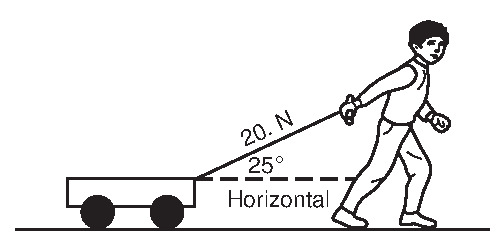
\includegraphics[keepaspectratio,scale=1.0]{Jan2007-Q45}
    \end{center}
    How much work does the child do in moving the wagon a horizontal distance of \SI{4.0}{\meter}?
    \begin{multicols}{2}
    \begin{choices}
      \correctchoice{\SI{73}{\joule}}
        \wrongchoice{\SI{5.0}{\joule}}
        \wrongchoice{\SI{80}{\joule}}
        \wrongchoice{\SI{34}{\joule}}
    \end{choices}
    \end{multicols}
\end{question}
}


%% Section June2006
%%--------------------
\element{nysed}{
\begin{question}{June2006-Q12}
    A \SI{2.0}{\kilo\gram} block sliding down a ramp from a height of \SI{3.0}{\meter} above the ground reaches the ground with a kinetic energy of \SI{50}{\joule}.
    The total work done by friction on the blocks as it slides down the ramp is approximately:
    \begin{multicols}{2}
    \begin{choices}
      \correctchoice{\SI{9}{\joule}}
        \wrongchoice{\SI{6}{\joule}}
        \wrongchoice{\SI{18}{\joule}}
        \wrongchoice{\SI{44}{\joule}}
    \end{choices}
    \end{multicols}
\end{question}
}

\element{nysed}{
\begin{question}{June2006-Q13}
    A person weighing \SI{6.0e2}{\newton} rides an elevator upward at an average speed of \SI{3.0}{\meter\per\second} for \SI{5.0}{\second}.
    How much does this person's gravitational potential energy increase as a result of this ride?
    \begin{multicols}{2}
    \begin{choices}
      \correctchoice{\SI{9e3}{\joule}}
        \wrongchoice{\SI{3e3}{\joule}}
        \wrongchoice{\SI{3.6e2}{\joule}}
        \wrongchoice{\SI{1.8e3}{\joule}}
    \end{choices}
    \end{multicols}
\end{question}
}

\element{nysed}{
\begin{question}{June2006-Q16}
    During an emergency stop, a \SI{1.5e3}{\kilo\gram} car lost a total of \SI{2.0e5}{\joule} of kinetic energy.
    What was the speed of the car at the moment the brakes were applied?
    \begin{multicols}{2}
    \begin{choices}
      \correctchoice{\SI{20}{\meter\per\second}}
        \wrongchoice{\SI{25}{\meter\per\second}}
        \wrongchoice{\SI{10.}{\meter\per\second}}
        \wrongchoice{\SI{14}{\meter\per\second}}
    \end{choices}
    \end{multicols}
\end{question}
}

\element{nysed}{
\begin{question}{June2006-Q41}
    Which two quantities can be expressed using same units?
    \begin{choices}
      \correctchoice{impulse and momentum}
        \wrongchoice{energy and force}
        \wrongchoice{impulse and force}
        \wrongchoice{momentum and energy}
    \end{choices}
\end{question}
}

\element{nysed}{
\begin{question}{June2006-Q45}
    A box is pushed to the right with a varying horizontal force.
    The graph below represents the relationship between the applied force and the distance the box moves.
    \begin{center}
    \begin{tikzpicture}
        \begin{axis}[
            axis y line=left,
            axis x line=bottom,
            axis line style={->},
            xlabel={distance},
            x unit=\si{\meter},
            xtick={0,3,6},
            ylabel={force},
            y unit=\si{\newton},
            ytick={0,3,6,9},
            xmin=0,xmax=6.5,
            ymin=0,ymax=6.5,
            grid=major,
            width=0.8\columnwidth,
            height=0.5\columnwidth,
            very thin,
        ]
        \addplot[line width=1pt,domain=0:3]{6};
        \addplot[line width=1pt,domain=3:6]{6 - 2*(x-3)};
        \end{axis}
    \end{tikzpicture}
    \end{center}
    What is the total work done in moving the box \SI{6.0}{\meter}?
    \begin{multicols}{2}
    \begin{choices}
      \correctchoice{\SI{27}{\joule}}
        \wrongchoice{\SI{36}{\joule}}
        \wrongchoice{\SI{9.0}{\joule}}
        \wrongchoice{\SI{18}{\joule}}
    \end{choices}
    \end{multicols}
\end{question}
}


%% Section Jan2006
%%--------------------
\element{nysed}{
\begin{question}{Jan2006-Q15}
    A \SI{6.8}{\kilo\gram} block is sliding down a horizontal,
        frictionless surface at a constant speed of \SI{6.0}{\meter\per\second}.
    The kinetic energy of the block is approximately:
    \begin{multicols}{2}
    \begin{choices}
      \correctchoice{\SI{120}{\joule}}
        \wrongchoice{\SI{20}{\joule}}
        \wrongchoice{\SI{41}{\joule}}
        \wrongchoice{\SI{240}{\joule}}
    \end{choices}
    \end{multicols}
\end{question}
}

\element{nysed}{
\begin{question}{Jan2006-Q16}
    Through what vertical distance is a \SI{50}{\newton} object moved if \SI{250}{\joule} of work is done against the gravitational field of Earth?
    \begin{multicols}{2}
    \begin{choices}
      \correctchoice{\SI{5.0}{\meter}}
        \wrongchoice{\SI{2.5}{\meter}}
        \wrongchoice{\SI{9.8}{\meter}}
        \wrongchoice{\SI{25}{\meter}}
    \end{choices}
    \end{multicols}
\end{question}
}

\element{nysed}{
\begin{question}{Jan2006-Q17}
    When a mass is placed on a spring with a spring constant of \SI{15}{\newton\per\meter},
        the spring is compressed \SI{0.25}{\meter}.
    How much elastic potential energy is stored in the spring?
    \begin{multicols}{2}
    \begin{choices}
      \correctchoice{\SI{0.47}{\joule}}
        \wrongchoice{\SI{0.94}{\joule}}
        \wrongchoice{\SI{1.9}{\joule}}
        \wrongchoice{\SI{3.8}{\joule}}
    \end{choices}
    \end{multicols}
\end{question}
}

\element{nysed}{
\begin{question}{Jan2006-Q18}
    Two students of equal weight go from the first floor to the second floor.
    The first student uses an elevator and the second student walks up a flight of stairs.
    compared to the gravitational potential energy gained by the first student,
        the gravitational potential energy gained by the second student is:
    \begin{multicols}{3}
    \begin{choices}
      \correctchoice{the same}
        \wrongchoice{less}
        \wrongchoice{greater}
    \end{choices}
    \end{multicols}
\end{question}
}

\element{nysed}{
\begin{question}{Jan2006-Q44}
    An object falls freely near Earth's surface.
    Which graph best represents the relationship between the object's kinetic energy and its time of fall?
    \begin{multicols}{2}
    \begin{choices}
        \AMCboxDimensions{down=-2.5em}
        \correctchoice{
            \begin{tikzpicture}
                \begin{axis}[
                    axis y line=left,
                    axis x line=bottom,
                    axis line style={->},
                    xlabel={time},
                    xtick=\empty,
                    ylabel={kinetic energy},
                    ytick=\empty,
                    xmin=0,xmax=10.5,
                    ymin=0.0,ymax=10.5,
                    width=0.98\columnwidth,
                    very thin,
                ]
                \addplot[line width=1pt,domain=0:10]{0.1*x*x};
                \end{axis}
            \end{tikzpicture}
        }
        \wrongchoice{
            \begin{tikzpicture}
                \begin{axis}[
                    axis y line=left,
                    axis x line=bottom,
                    axis line style={->},
                    xlabel={time},
                    xtick=\empty,
                    ylabel={kinetic energy},
                    ytick=\empty,
                    xmin=0,xmax=10.5,
                    ymin=0.0,ymax=10.5,
                    width=0.98\columnwidth,
                    very thin,
                ]
                \addplot[line width=1pt,domain=0:10]{x};
                \end{axis}
            \end{tikzpicture}
        }
        \wrongchoice{
            \begin{tikzpicture}
                \begin{axis}[
                    axis y line=left,
                    axis x line=bottom,
                    axis line style={->},
                    xlabel={time},
                    xtick=\empty,
                    ylabel={kinetic energy},
                    ytick=\empty,
                    xmin=0,xmax=10.5,
                    ymin=0.0,ymax=10.5,
                    width=0.98\columnwidth,
                    very thin,
                ]
                \addplot[line width=1pt,domain=0:10]{10-x};
                \end{axis}
            \end{tikzpicture}
        }
        \wrongchoice{
            \begin{tikzpicture}
                \begin{axis}[
                    axis y line=left,
                    axis x line=bottom,
                    axis line style={->},
                    xlabel={time},
                    xtick=\empty,
                    ylabel={kinetic energy},
                    ytick=\empty,
                    xmin=0,xmax=10.5,
                    ymin=0.0,ymax=10.5,
                    width=0.98\columnwidth,
                    very thin,
                ]
                \addplot[line width=1pt,domain=0:10]{10-0.1*x*x};
                \end{axis}
            \end{tikzpicture}
        }
    \end{choices}
    \end{multicols}
\end{question}
}


%% Section June2005
%%--------------------
\element{nysed}{
\begin{question}{June2005-Q16}
    As shown in the diagram below,
        a student exerts an average force of \SI{600}{\newton} on a rope to lift a \SI{50}{\kilo\gram} crate a vertical distance of \SI{3.00}{\meter}.
    \begin{center}
        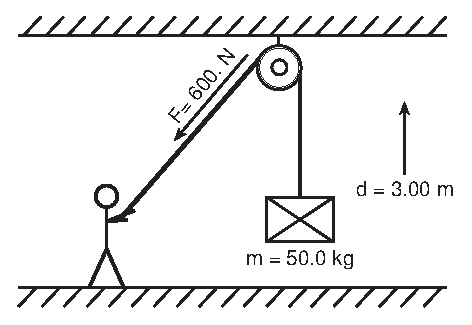
\includegraphics[keepaspectratio,scale=0.75]{June2005-Q16}
    \end{center}
    Compared to the work done by the student,
        the gravitational potential energy gained by the crate is:
    \begin{choices}
      \correctchoice{exactly the same}
        \wrongchoice{\SI{330}{\joule} less}
        \wrongchoice{\SI{330}{\joule} more}
        \wrongchoice{\SI{150}{\joule} more}
    \end{choices}
\end{question}
}

\element{nysed}{
\begin{question}{June2005-Q17}
    A \SI{1.0}{\kilo\gram} book resting on the ground is moved \SI{1.0}{\meter} at various angles relative to the horizontal.
    In which direction does the \SI{1.0}{\meter} displacement produce the greatest increase in the book's gravitational potential energy?
    \begin{multicols}{2}
    \begin{choices}\footnotesize
        \AMCboxDimensions{down=-0.7cm}
        \correctchoice{
            \begin{tikzpicture}
                %% Book
                \draw[white] (-1.5,0) rectangle (1.5,2);
                \node[draw,rectangle,minimum size=1.00cm,anchor=center]
                    (B) at (-0.5,0.5) {Book};
                %% Vector
                \draw[thick,->] (B.north) -- ++(90:1) node[pos=0.0,anchor=south west] {\ang{90}};
                %% Floor
                \draw[thick] (-1.5,0) -- (1.5,0);
                \node[anchor=north,pattern=north east lines,minimum width=3cm] at (0,0) {};
                \node[anchor=north] at (-0.5,-1em) {Ground};
            \end{tikzpicture}
        }
        \wrongchoice{
            \begin{tikzpicture}
                %% Book
                \draw[white] (-1.5,0) rectangle (1.5,2);
                \node[draw,rectangle,minimum size=1.00cm,anchor=center]
                    (B) at (-0.5,0.5) {Book};
                %% Vector
                \draw[thick,->] (B.north east) -- ++(45:1);
                \draw[thick,dotted,<->] (1.0,0) arc (0:45:2.0) node[pos=0.5,anchor=west] {\ang{45}};
                %% Floor
                \draw[thick] (-1.5,0) -- (1.5,0);
                \node[anchor=north,pattern=north east lines,minimum width=3cm] at (0,0) {};
                \node[anchor=north] at (-0.5,-1em) {Ground};
            \end{tikzpicture}
        }
        \wrongchoice{
            \begin{tikzpicture}
                %% Book
                \draw[white] (-1.5,0) rectangle (1.5,2);
                \node[draw,rectangle,minimum size=1.00cm,anchor=center]
                    (B) at (-0.5,0.5) {Book};
                %% Vector
                \draw[thick,->] (B.east) -- ++(20:1);
                \draw[thick,dotted,<->] (0.66,0) arc (0:20:2.04) node[pos=0.5,anchor=west] {\ang{20}};
                %% Floor
                \draw[thick] (-1.5,0) -- (1.5,0);
                \node[anchor=north,pattern=north east lines,minimum width=3cm] at (0,0) {};
                \node[anchor=north] at (-0.5,-1em) {Ground};
            \end{tikzpicture}
        }
        \wrongchoice{
            \begin{tikzpicture}
                %% Book
                \draw[white] (-1.5,0) rectangle (1.5,2);
                \node[draw,rectangle,minimum size=1.00cm,anchor=center]
                    (B) at (-0.5,0.5) {Book};
                %% Vector
                \draw[->] (B.east) -- ++(0:1) node[pos=0.0,anchor=south west] {\ang{0}};
                %% Floor
                \draw[thick] (-1.5,0) -- (1.5,0);
                \node[anchor=north,pattern=north east lines,minimum width=3cm] at (0,0) {};
                \node[anchor=north] at (-0.5,-1em) {Ground};
            \end{tikzpicture}
        }
    \end{choices}
    \end{multicols}
\end{question}
}


%% Section Jan2005
%%--------------------
\element{nysed}{
\begin{question}{Jan2005-Q20}
    What is the gravitational energy with respect to the surface of the water of a \SI{75.0}{\kilo\gram} diver located \SI{3.00}{\meter} above the water?
    \begin{multicols}{2}
    \begin{choices}
      \correctchoice{\SI{2.21e3}{\joule}}
        \wrongchoice{\SI{2.17e4}{\joule}}
        \wrongchoice{\SI{2.25e2}{\joule}}
        \wrongchoice{\SI{2.29e1}{\joule}}
    \end{choices}
    \end{multicols}
\end{question}
}

\element{nysed}{
\begin{question}{Jan2005-Q21}
    A \SI{60.0}{\kilo\gram} runner has \SI{1920}{\joule} of kinetic energy.
    At what speed is she running?
    \begin{multicols}{2}
    \begin{choices}
      \correctchoice{\SI{8.00}{\meter\per\second}}
        \wrongchoice{\SI{5.66}{\meter\per\second}}
        \wrongchoice{\SI{32.0}{\meter\per\second}}
        \wrongchoice{\SI{64.0}{\meter\per\second}}
    \end{choices}
    \end{multicols}
\end{question}
}

\element{nysed}{
\begin{question}{Jan2005-Q22}
    The diagram below shows points $A$, $B$, and $C$ at or near the Earth's surface.
    As a mass is moved from $A$ to $B$, \SI{100}{\joule} of work are done against gravity.
    \begin{center}
    \begin{tikzpicture}
        %% Earth's surface
        \draw[thick] (-4,0) -- (4,0) node[pos=0.5,anchor=north] {Earth's surface};
        %% Point A, B, C
        \draw[fill] (-3,0) circle (1.5pt) node[anchor=north] {$A$};
        \draw[fill] (-3,3) circle (1.5pt) node[anchor=south] {$B$};
        \draw[fill] (+3,3) circle (1.5pt) node[anchor=south] {$C$};
        %% 10 meter labels
        \draw[thick,<->] (-3,0) -- (-3,3) node[pos=0.5,anchor=center,rotate=90,fill=white] {\SI{10}{\meter}};
        \draw[thick,<->] (+3,0) -- (+3,3) node[pos=0.5,anchor=center,rotate=90,fill=white] {\SI{10}{\meter}};
        %% 20 meter labels
        \draw[thick,<->] (-3,0) -- (+3,3) node[pos=0.5,anchor=center,rotate=26.6,fill=white] {\SI{20}{\meter}};
    \end{tikzpicture}
    \end{center}
    What is the amount of work done against gravity as an identical mass is moved from $A$ to $C$?
    \begin{multicols}{2}
    \begin{choices}
      \correctchoice{\SI{100}{\joule}}
        \wrongchoice{\SI{200}{\joule}}
        \wrongchoice{\SI{173}{\joule}}
        \wrongchoice{\SI{273}{\joule}}
    \end{choices}
    \end{multicols}
\end{question}
}

\element{nysed}{
\begin{question}{Jan2005-Q23}
    When a force moves an object over a rough,
        horizontal surface at constant velocity,
        the work done against friction produces an increase in the object's:
    \begin{multicols}{2}
    \begin{choices}
      \correctchoice{internal energy}
        \wrongchoice{weight}
        \wrongchoice{potential energy}
        \wrongchoice{internal energy}
    \end{choices}
    \end{multicols}
\end{question}
}


%% Section June2004
%%--------------------
\element{nysed}{
\begin{question}{June2004-Q11}
    The work done in moving a block across a rough surface and the heat energy gained by the block can both be measured in:
    \begin{multicols}{2}
    \begin{choices}
      \correctchoice{joules}
        \wrongchoice{degrees}
        \wrongchoice{newtons}
        \wrongchoice{watts}
    \end{choices}
    \end{multicols}
\end{question}
}

\element{nysed}{
\begin{question}{June2004-Q12}
    Two weightlifters, one \SI{1.5}{\meter} tall and one \SI{2.0}{\meter} tall,
        raise identical \SI{50}{\kilo\gram} masses above their heads.
    Compared to the work done by the weightlifter who is \SI{1.5}{\meter} tall,
        the work done by the weightlifter who is \SI{2.0}{\meter} tall is:
    \begin{multicols}{3}
    \begin{choices}
      \correctchoice{greater}
        \wrongchoice{less}
        \wrongchoice{the same}
    \end{choices}
    \end{multicols}
\end{question}
}

\element{nysed}{
\begin{question}{June2004-Q13}
    A \SI{45}{\kilo\gram} boy is riding a \SI{15}{\kilo\gram} bicycle with a speed of \SI{8.00}{\meter\per\second}.
    What is the combined kinetic energy of the boy and the bicycle?
    \begin{multicols}{2}
    \begin{choices}
      \correctchoice{\SI{1920}{\joule}}
        \wrongchoice{\SI{1440}{\joule}}
        \wrongchoice{\SI{480}{\joule}}
        \wrongchoice{\SI{240}{\joule}}
    \end{choices}
    \end{multicols}
\end{question}
}


%% Section Jan2004
%%--------------------
\element{nysed}{
\begin{question}{Jan2004-Q18}
    A student does \SI{60}{\joule} of work pushing a \SI{3.0}{\kilo\gram} box up the full length of a ramp that is \SI{5.0}{\meter} long.
    What is the magnitude of the force applied to the box to do this work?
    \begin{multicols}{2}
    \begin{choices}
      \correctchoice{\SI{12}{\newton}}
        \wrongchoice{\SI{15}{\newton}}
        \wrongchoice{\SI{4.0}{\newton}}
        \wrongchoice{\SI{20.}{\newton}}
    \end{choices}
    \end{multicols}
\end{question}
}


%% Section June2003
%%--------------------
\element{nysed}{
\begin{question}{June2003-Q01}
    The diagram below shows a \SI{40}{\kilo\gram} crate on a frictionless plane at angle $\theta$ to the horizontal.
    The crate is pushed at constant speed up the incline from point $A$ to point $B$ by force $F$.
    \begin{center}
    \begin{tikzpicture}
        %% Ramp
        \draw[thick] (0,0) -- (20:6);
        %% A and B Label
        \draw[fill] (20:0) circle  (1.5pt)
            node[anchor=north] {$A$};
        \draw[fill] (20:5) circle  (1.5pt)
            node[anchor=north] {$B$};
        %% Theta label
        \draw[thick,<->,dashed] (0:2) arc (0:20:2)
            node[pos=0.5,anchor=west] {$\theta$};
        %% Block
        \node[draw,rectangle,minimum size=0.75cm,rotate=20,anchor=south west]
            (B) at (20:0) {\SI{50}{\kilo\gram}};
        \draw[thick,<-] (B.west) -- ++ (200:1)
            node[pos=0.66,anchor=south] {$F$};
        %% Horizontal
        \draw[thick] (0:0) -- (0:5.7)
            node[pos=0.5,anchor=north] {horizontal};
    \end{tikzpicture}
    \end{center}
    If angle $\theta$ were increased, what would be the effect on the magnitude of force $F$ and the total work $W$ done on the create as it is moved from $A$ to $B$.
    The worker's pull on the handle of the cart can best be described as a force having:
    \begin{choices}
      \correctchoice{$W$ would increase and the magnitude of $F$ would increase.}
        \wrongchoice{$W$ would remain the same and the magnitude of $F$ would decrease.}
        \wrongchoice{$W$ would remain the same and the magnitude of $F$ would increase.}
        \wrongchoice{$W$ would increase and the magnitude of $F$ would decrease.}
    \end{choices}
\end{question}
}

\element{nysed}{
\begin{question}{June2003-Q10}
    A \SI{10}{\newton} force is required to hold a stretched spring \SI{0.20}{\meter} from its rest position.
    What is the potential energy stored in the stretched spring?
    \begin{multicols}{2}
    \begin{choices}
      \correctchoice{\SI{1.0}{\joule}}
        \wrongchoice{\SI{2.0}{\joule}}
        \wrongchoice{\SI{5.0}{\joule}}
        \wrongchoice{\SI{50}{\joule}}
    \end{choices}
    \end{multicols}
\end{question}
}


%% Section Jan2003
%%--------------------
\element{nysed}{
\begin{question}{Jan2003-Q12}
    The amount of work done against friction to slide a box in a straight line across a uniform,
        horizontal floor depends most on the:
    \begin{choices}
      \correctchoice{distance taken to move the box}
        \wrongchoice{time taken to move the box}
        \wrongchoice{speed of the box}
        \wrongchoice{direction of the box's motion}
    \end{choices}
\end{question}
}

\element{nysed}{
\begin{question}{Jan2003-Q13}
    A \SI{1.2}{\kilo\gram} block and a \SI{1.8}{\kilo\gram} block are initially at rest on a frictionless, horizontal surface.
    When a compressed spring between the blocks is released,
        the \SI{1.8}{\kilo\gram} block moves to the right at \SI{2.0}{\meter\per\second} as shown.
    \begin{center}
    \begin{tikzpicture}
        %% Floor
        \draw (-4,0) -- (4,0);
        \node[anchor=north,fill,pattern=north east lines,minimum width=8cm, minimum height=0.05cm] at (0,0) {};
        \node[anchor=north] at (0,-0.25) {Frictionless horizontal surface};
        %% blocks
        \node[anchor=south,draw,minimum size=1.5cm,fill=white!90!black] (L) at (-2,0) {\SI{1.2}{\kilo\gram}};
        \node[anchor=south,draw,minimum size=1.5cm,fill=white!90!black] (R) at (+2,0) {\SI{1.8}{\kilo\gram}};
        %% velocity
        \draw[thick,->] (L.north east) ++(90:0.5) -- ++(180:1.5cm) node[pos=0.5,anchor=south] {?};
        \draw[thick,->] (R.north west) ++(90:0.5) -- ++(0:1.5cm) node[pos=0.5,anchor=south] {\SI{2.0}{\meter\per\second}};
        %% Spring
        \draw[thick,decoration={aspect=0.2,segment length=2mm,amplitude=4mm,coil},decorate] (L.east) -- (R.west);
    \end{tikzpicture}
    \end{center}
    What is the speed of the \SI{1.2}{\kilo\gram} block after the spring is released?
    \begin{multicols}{2}
    \begin{choices}
      \correctchoice{\SI{3.0}{\meter\per\second}}
        \wrongchoice{\SI{1.4}{\meter\per\second}}
        \wrongchoice{\SI{2.0}{\meter\per\second}}
        \wrongchoice{\SI{3.6}{\meter\per\second}}
    \end{choices}
    \end{multicols}
\end{question}
}

\element{nysed}{
\begin{question}{Jan2003-Q15}
    An object weighs \SI{15}{\newton} is listed from the ground of \SI{0.22}{\meter}.
    The increase in the object's gravitational potential energy is approximately:
    \begin{multicols}{2}
    \begin{choices}
      \correctchoice{\SI{3.3}{\joule}}
        \wrongchoice{\SI{33}{\joule}}
        \wrongchoice{\SI{310}{\joule}}
        \wrongchoice{\SI{0.34}{\joule}}
    \end{choices}
    \end{multicols}
\end{question}
}

\element{nysed}{
\begin{question}{Jan2003-Q41}
    The spring of a toy car is wound by pushing the car backward with an average force of \SI{15}{\newton} through a distance of \SI{0.50}{\meter}.
    How much elastic potential energy is stored in the car's spring during this process?
    \begin{multicols}{2}
    \begin{choices}
      \correctchoice{\SI{7.5}{\joule}}
        \wrongchoice{\SI{1.9}{\joule}}
        \wrongchoice{\SI{30}{\joule}}
        \wrongchoice{\SI{56}{\joule}}
    \end{choices}
    \end{multicols}
\end{question}
}


%% Section Aug2002
%%--------------------
\element{nysed}{
\begin{question}{Aug2002-Q08}
    A block weighing \SI{15}{\newton} is pulled to the top of an incline that is \SI{0.20}{\meter} above the ground, as shown below.
    \begin{center}
    \begin{tikzpicture}
        %% plane
        \draw (0,0) -- (30:6) --++(270:3) -- cycle;
        %% block
        \node[anchor=south,rotate=30,draw,minimum size=1cm] (A) at (30:1) {\SI{15}{\newton}};
        %% force
        \draw[thick,->] (A.east) -- ++(30:1.5);
        %% height
        \draw[<->] (30:6) ++(0:1) -- ++(270:3) node[pos=0.5,anchor=center,fill=white] {\SI{0.20}{\meter}};
    \end{tikzpicture}
    \end{center}
    If \SI{4.0}{\joule} of work are needed to pull the block the full length of the incline,
        how much work is done against friction?
    \begin{multicols}{2}
    \begin{choices}
      \correctchoice{\SI{1.0}{\joule}}
        \wrongchoice{\SI{0.0}{\joule}}
        \wrongchoice{\SI{3.0}{\joule}}
        \wrongchoice{\SI{7.0}{\joule}}
    \end{choices}
    \end{multicols}
\end{question}
}

\element{nysed}{
\begin{question}{Aug2002-Q09}
    A \SI{1.0}{\kilo\gram} rubber ball traveling east at \SI{4.0}{\meter\per\second} hits a wall and bounces back toward the west at \SI{2.0}{\meter\per\second}.
    Compared to the kinetic energy of the ball before it hits the wall,
        the kinetic energy of the ball after it bounces off the wall is:
    \begin{choices}
      \correctchoice{one-fourth as great}
        \wrongchoice{one-half as great}
        \wrongchoice{the same}
        \wrongchoice{four times as great}
    \end{choices}
\end{question}
}

\element{nysed}{
\begin{question}{Aug2002-Q10}
    As a spring is stretched,
        its elastic potential energy:
    \begin{choices}
        \wrongchoice{decreases}
      \correctchoice{increases}
        \wrongchoice{remains the same}
    \end{choices}
\end{question}
}

\element{nysed}{
\begin{question}{Aug2002-Q12}
    A catapult with a spring constant of \SI{1.0e4}{\newton\per\meter} is required to launch an airplane from the deck of an aircraft carrier.
    The plane is released when it has been displaced \SI{0.50}{\meter} from its equilibrium position by the catapult.
    The energy acquired by the airplane from the catapult during takeoff is approximately:
    \begin{multicols}{2}
    \begin{choices}
      \correctchoice{\SI{1.3e3}{\joule}}
        \wrongchoice{\SI{2.0e4}{\joule}}
        \wrongchoice{\SI{2.5e3}{\joule}}
        \wrongchoice{\SI{1.0e4}{\joule}}
    \end{choices}
    \end{multicols}
\end{question}
}


%% Section June2002
%%--------------------
\element{nysed}{
\begin{question}{June2002-Q20}
    In the diagram below, \SI{400}{\joule} of work is done raising a \SI{72}{\newton} weight a vertical distance of \SI{5.0}{\meter}.
    \begin{center}
        %% NOTE: TODO: draw tikz
        %% NOTE: check cpo for pulley
        %% NOTE: this pulley is more involved.
        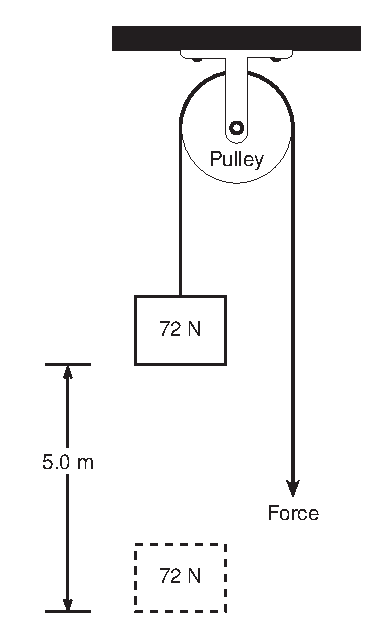
\includegraphics[keepaspectratio,scale=0.75]{June2002-Q20}
    \end{center}
    How much work is done to overcome friction as the weight is raised?
    \begin{multicols}{2}
    \begin{choices}
      \correctchoice{\SI{40}{\joule}}
        \wrongchoice{\SI{400}{\joule}}
        \wrongchoice{\SI{360}{\joule}}
        \wrongchoice{\SI{760}{\joule}}
    \end{choices}
    \end{multicols}
\end{question}
}

\element{nysed}{
\begin{question}{June2002-Q14}
    An object moving at a constant speed of \SI{25}{\meter\per\second} possesses \SI{450}{\joule} of kinetic energy.
    What is the object's mass?
    \begin{multicols}{2}
    \begin{choices}
        \wrongchoice{\SI{0.72}{\kilo\gram}}
      \correctchoice{\SI{1.4}{\kilo\gram}}
        \wrongchoice{\SI{18}{\kilo\gram}}
        \wrongchoice{\SI{36}{\kilo\gram}}
    \end{choices}
    \end{multicols}
\end{question}
}

\element{nysed}{
\begin{question}{June2002-Q15}
    The diagram below shows a moving,
        \SI{5.0}{\kilo\gram} cart at the foot of a hill, \SI{10.0}{\meter} high.
    \begin{center}
    \begin{tikzpicture}
        %% Ground
        \draw[dashed] (-2,0) -- (4,0);
        \draw[very thick] (-4,0) -- (-2,0) to[out=0,in=180] (2,2) -- (4,2);
        \draw[<->] (3.5,0) -- (3.5,2) node[pos=0.5,anchor=center,fill=white] {\SI{10.0}{\meter}};
        %% Cart
        \node[draw,fill=white!90!black,minimum height=1.00cm,minimum width=2.00cm,anchor=south] (A) at (-3,0.2) {\SI{5.00}{\kilo\gram}};
        \draw[very thick,->] (A.north west) ++(90:0.5) -- ++(0:2cm) node[pos=0.5,anchor=south] {$v$};
        %% wheels
        \draw[fill=white] (A.south west) ++(0:0.3) circle (0.2);
        \draw[fill=black] (A.south west) ++(0:0.3) circle (1pt);
        \draw[fill=white] (A.south east) ++(180:0.3) circle (0.2);
        \draw[fill=black] (A.south east) ++(180:0.3) circle (1pt);
    \end{tikzpicture}
    \end{center}
    For the cart to reach the top of the hill,
        what is the minimum kinetic energy of the cart in the position shown?
    [Neglect energy loss due to friction]
    \begin{multicols}{2}
    \begin{choices}
        \wrongchoice{\SI{4.91}{\joule}}
        \wrongchoice{\SI{50.0}{\joule}}
      \correctchoice{\SI{250}{\joule}}
        \wrongchoice{\SI{491}{\joule}}
    \end{choices}
    \end{multicols}
\end{question}
}

\element{nysed}{
\begin{question}{June2002-Q16}
    A constant force of \SI{1900}{\newton} is required to keep an automobile having a mass of \SI{1.0e3}{\kilo\gram} moving at a constant speed of \SI{20}{\meter\per\second}.
    The work done in moving the automobile a distance of \SI{2.0e3}{\meter} is:
    \begin{multicols}{2}
    \begin{choices}
        \wrongchoice{\SI{2.0e4}{\joule}}
        \wrongchoice{\SI{3.8e4}{\joule}}
        \wrongchoice{\SI{2.0e6}{\joule}}
      \correctchoice{\SI{3.8e6}{\joule}}
    \end{choices}
    \end{multicols}
\end{question}
}

\element{nysed}{
\begin{question}{June2002-Q33}
    A spring of negligible mass has a spring constant of \SI{50}{\newton\per\meter}.
    If the spring is stretched \SI{0.40}{\meter} from its equilibrium position,
        how much potential energy is stored in the spring?
    \begin{multicols}{2}
    \begin{choices}
        \wrongchoice{\SI{20}{\joule}}
        \wrongchoice{\SI{10}{\joule}}
        \wrongchoice{\SI{8.0}{\joule}}
      \correctchoice{\SI{4.0}{\joule}}
    \end{choices}
    \end{multicols}
\end{question}
}

\element{nysed}{
\begin{question}{June2002-Q42}
    Which graph best represents the elastic potential energy stored in a spring as a function of its elongation?
    \begin{multicols}{2}
    \begin{choices}
        \AMCboxDimensions{down=-2.5em}
        \correctchoice{
            \begin{tikzpicture}
                \begin{axis}[
                    axis y line=left,
                    axis x line=bottom,
                    axis line style={->},
                    xlabel={elongation},
                    xtick=\empty,
                    ylabel={energy},
                    ytick=\empty,
                    xmin=0,xmax=11,
                    ymin=0,ymax=11,
                    width=0.98\columnwidth,
                    very thin,
                ]
                \addplot[line width=1pt,domain=0:10]{0.1*x*x};
                \end{axis}
            \end{tikzpicture}
        }
        \wrongchoice{
            \begin{tikzpicture}
                \begin{axis}[
                    axis y line=left,
                    axis x line=bottom,
                    axis line style={->},
                    xlabel={elongation},
                    xtick=\empty,
                    ylabel={energy},
                    ytick=\empty,
                    xmin=0,xmax=10.5,
                    ymin=0,ymax=10.5,
                    width=0.98\columnwidth,
                    very thin,
                ]
                \addplot[line width=1pt,domain=0:10]{x};
                \end{axis}
            \end{tikzpicture}
        }
        \wrongchoice{
            \begin{tikzpicture}
                \begin{axis}[
                    axis y line=left,
                    axis x line=bottom,
                    axis line style={->},
                    xlabel={elongation},
                    xtick=\empty,
                    ylabel={energy},
                    ytick=\empty,
                    xmin=0,xmax=11,
                    ymin=0,ymax=11,
                    width=0.98\columnwidth,
                    very thin,
                ]
                \addplot[line width=1pt,domain=0:10]{10-x};
                \end{axis}
            \end{tikzpicture}
        }
        \wrongchoice{
            \begin{tikzpicture}
                \begin{axis}[
                    axis y line=left,
                    axis x line=bottom,
                    axis line style={->},
                    xlabel={elongation},
                    xtick=\empty,
                    ylabel={energy},
                    ytick=\empty,
                    xmin=0,xmax=11,
                    ymin=0,ymax=11,
                    width=0.98\columnwidth,
                    very thin,
                ]
                \addplot[line width=1pt,domain=0:10]{10/x};
                \end{axis}
            \end{tikzpicture}
        }
    \end{choices}
    \end{multicols}
\end{question}
}

\element{nysed}{
\begin{question}{June2002-Q43}
    Which graph best represents the relationship between the gravitational potential energy of a freely falling object and the object's height above the ground near the surface of Earth?
    \begin{multicols}{2}
    \begin{choices}
        \AMCboxDimensions{down=-2.5em}
        \correctchoice{
            \begin{tikzpicture}
                \begin{axis}[
                    axis y line=left,
                    axis x line=bottom,
                    axis line style={->},
                    xlabel={height},
                    xtick=\empty,
                    ylabel={energy},
                    ytick=\empty,
                    xmin=0,xmax=10.5,
                    ymin=0,ymax=10.5,
                    width=0.98\columnwidth,
                    very thin,
                ]
                \addplot[line width=1pt,domain=0:10]{x};
                \end{axis}
            \end{tikzpicture}
        }
        \wrongchoice{
            \begin{tikzpicture}
                \begin{axis}[
                    axis y line=left,
                    axis x line=bottom,
                    axis line style={->},
                    xlabel={height},
                    xtick=\empty,
                    ylabel={energy},
                    ytick=\empty,
                    xmin=0,xmax=11,
                    ymin=0,ymax=11,
                    width=0.98\columnwidth,
                    very thin,
                ]
                \addplot[line width=1pt,domain=0:10]{0.1*x*x};
                \end{axis}
            \end{tikzpicture}
        }
        \wrongchoice{
            \begin{tikzpicture}
                \begin{axis}[
                    axis y line=left,
                    axis x line=bottom,
                    axis line style={->},
                    xlabel={height},
                    xtick=\empty,
                    ylabel={energy},
                    ytick=\empty,
                    xmin=0,xmax=11,
                    ymin=0,ymax=11,
                    width=0.98\columnwidth,
                    very thin,
                ]
                \addplot[line width=1pt,domain=0:10]{10-x};
                \end{axis}
            \end{tikzpicture}
        }
        \wrongchoice{
            \begin{tikzpicture}
                \begin{axis}[
                    axis y line=left,
                    axis x line=bottom,
                    axis line style={->},
                    xlabel={height},
                    xtick=\empty,
                    ylabel={energy},
                    ytick=\empty,
                    xmin=0,xmax=11,
                    ymin=0,ymax=11,
                    width=0.98\columnwidth,
                    very thin,
                ]
                \addplot[line width=1pt,domain=0:10]{8};
                \end{axis}
            \end{tikzpicture}
        }
    \end{choices}
    \end{multicols}
\end{question}
}


%% Section Jan2002
%%--------------------
\element{nysed}{
\begin{question}{Jan2002-Q18}
    Which graph best represents the relationship between the kinetic energy of a moving object and its velocity?
    \begin{multicols}{2}
    \begin{choices}
        \AMCboxDimensions{down=-2.5em}
        \correctchoice{
            \begin{tikzpicture}
                \begin{axis}[
                    axis y line=left,
                    axis x line=bottom,
                    axis line style={->},
                    xlabel={velocity},
                    xtick=\empty,
                    ylabel={kinetic energy},
                    ytick=\empty,
                    xmin=0,xmax=10.5,
                    ymin=0.0,ymax=10.5,
                    width=0.98\columnwidth,
                    very thin,
                ]
                \addplot[line width=1pt,domain=0:10]{0.1 *x*x};
                \end{axis}
            \end{tikzpicture}
        }
        \wrongchoice{
            \begin{tikzpicture}
                \begin{axis}[
                    axis y line=left,
                    axis x line=bottom,
                    axis line style={->},
                    xlabel={velocity},
                    xtick=\empty,
                    ylabel={kinetic energy},
                    ytick=\empty,
                    xmin=0,xmax=10.5,
                    ymin=0.0,ymax=10.5,
                    width=0.98\columnwidth,
                    very thin,
                ]
                \addplot[line width=1pt,domain=0:10]{8};
                \end{axis}
            \end{tikzpicture}
        }
        \wrongchoice{
            \begin{tikzpicture}
                \begin{axis}[
                    axis y line=left,
                    axis x line=bottom,
                    axis line style={->},
                    xlabel={velocity},
                    xtick=\empty,
                    ylabel={kinetic energy},
                    ytick=\empty,
                    xmin=0,xmax=10.5,
                    ymin=0.0,ymax=10.5,
                    width=0.98\columnwidth,
                    very thin,
                ]
                \addplot[line width=1pt,domain=0:10]{x};
                \end{axis}
            \end{tikzpicture}
        }
        \wrongchoice{
            \begin{tikzpicture}
                \begin{axis}[
                    axis y line=left,
                    axis x line=bottom,
                    axis line style={->},
                    xlabel={velocity},
                    xtick=\empty,
                    ylabel={kinetic energy},
                    ytick=\empty,
                    xmin=0,xmax=10.5,
                    ymin=0.0,ymax=10.5,
                    width=0.98\columnwidth,
                    very thin,
                ]
                \addplot[line width=1pt,domain=0:10]{10/x};
                \end{axis}
            \end{tikzpicture}
        }
    \end{choices}
    \end{multicols}
\end{question}
}

\element{nysed}{
\begin{question}{Jan2002-Q19}
    How much work is done on a downhill skier by an average braking force of \SI{9.8e2}{\newton} to stop her in a distance of \SI{10}{\meter}?
    \begin{multicols}{2}
    \begin{choices}
        \wrongchoice{\SI{1.0e1}{\joule}}
        \wrongchoice{\SI{9.8e1}{\joule}}
        \wrongchoice{\SI{1.0e3}{\joule}}
      \correctchoice{\SI{9.8e3}{\joule}}
    \end{choices}
    \end{multicols}
\end{question}
}

\element{nysed}{
\begin{question}{Jan2002-Q20}
    A spring has a spring constant of \SI{120}{\newton\per\meter}.
    How much potential energy is stored in the spring as it is stretched \SI{0.20}{\meter}?
    \begin{multicols}{2}
    \begin{choices}
      \correctchoice{\SI{2.4}{\joule}}
        \wrongchoice{\SI{4.8}{\joule}}
        \wrongchoice{\SI{12}{\joule}}
        \wrongchoice{\SI{24}{\joule}}
    \end{choices}
    \end{multicols}
\end{question}
}

\element{nysed}{
\begin{question}{Jan2002-Q22}
    Which quantity and unit are correctly paired?
    \begin{choices}
        \wrongchoice{velocity---\si{\meter\per\second\squared}}
        \wrongchoice{momentum---\si{\kilo\gram\meter\per\second\squared}}
      \correctchoice{energy---\si{\kilo\gram\meter\squared\per\second\squared}}
        \wrongchoice{work---\si{\kilo\gram\per\meter}}
    \end{choices}
\end{question}
}

\element{nysed}{
\begin{question}{Jan2002-Q24}
    A \SI{0.10}{\kilo\gram} ball dropped vertically from a height of \SI{1.00}{\meter} above the floor bounces back to a height of \SI{0.80}{\meter}.
    The mechanical energy lost by the ball as it bounces is:
    \begin{multicols}{2}
    \begin{choices}
        \wrongchoice{\SI{0.080}{\joule}}
      \correctchoice{\SI{0.20}{\joule}}
        \wrongchoice{\SI{0.30}{\joule}}
        \wrongchoice{\SI{0.78}{\joule}}
    \end{choices}
    \end{multicols}
\end{question}
}


%% Section June2001
%%--------------------
\element{nysed}{
\begin{question}{June2001-Q16}
    Which combination of units can be used to express work?
    \begin{choices}
        \wrongchoice{newton second per meter (\si{\newton\second\per\meter})}
        \wrongchoice{newton meter per second (\si{\newton\meter\per\second})}
        \wrongchoice{newton per meter (\si{\newton\per\meter})}
      \correctchoice{newton meter (\si{\newton\meter})}
    \end{choices}
\end{question}
}

\element{nysed}{
\begin{question}{June2001-Q18}
    Which graph best represents the relationship between gravitational potential energy and height above the ground for an object near the surface of Earth?
    \begin{multicols}{2}
    \begin{choices}
        \AMCboxDimensions{down=-2.5em}
        \correctchoice{
            \begin{tikzpicture}
                \begin{axis}[
                    axis y line=left,
                    axis x line=bottom,
                    axis line style={->},
                    xlabel={height},
                    xtick=\empty,
                    ylabel={potential energy},
                    ytick=\empty,
                    xmin=0,xmax=10.5,
                    ymin=0.0,ymax=10.5,
                    width=0.98\columnwidth,
                    very thin,
                ]
                \addplot[line width=1pt,domain=0:10]{x};
                \end{axis}
            \end{tikzpicture}
        }
        \wrongchoice{
            \begin{tikzpicture}
                \begin{axis}[
                    axis y line=left,
                    axis x line=bottom,
                    axis line style={->},
                    xlabel={height},
                    xtick=\empty,
                    ylabel={potential energy},
                    ytick=\empty,
                    xmin=0,xmax=10.5,
                    ymin=0.0,ymax=10.5,
                    width=0.98\columnwidth,
                    very thin,
                ]
                \addplot[line width=1pt,domain=0:10]{8};
                \end{axis}
            \end{tikzpicture}
        }
        \wrongchoice{
            \begin{tikzpicture}
                \begin{axis}[
                    axis y line=left,
                    axis x line=bottom,
                    axis line style={->},
                    xlabel={height},
                    xtick=\empty,
                    ylabel={potential energy},
                    ytick=\empty,
                    xmin=0,xmax=10.5,
                    ymin=0.0,ymax=10.5,
                    width=0.98\columnwidth,
                    very thin,
                ]
                \addplot[line width=1pt,domain=0:10]{0.1 *x*x};
                \end{axis}
            \end{tikzpicture}
        }
        \wrongchoice{
            \begin{tikzpicture}
                \begin{axis}[
                    axis y line=left,
                    axis x line=bottom,
                    axis line style={->},
                    xlabel={height},
                    xtick=\empty,
                    ylabel={potential energy},
                    ytick=\empty,
                    xmin=0,xmax=10.5,
                    ymin=0.0,ymax=10.5,
                    width=0.98\columnwidth,
                    very thin,
                ]
                \addplot[line width=1pt,domain=0:10]{10/x};
                \end{axis}
            \end{tikzpicture}
        }
    \end{choices}
    \end{multicols}
\end{question}
}

\element{nysed}{
\begin{question}{June2001-Q20}
    A \SI{3.0}{\newton} mass is attached to a spring having a spring constant of \SI{30}{\newton\per\meter}.
    The mass is pulled \SI{0.20}{\meter} from the spring's equilibrium position and released.
    What is the maximum kinetic energy achieved by the mass-spring system?
    \begin{multicols}{2}
    \begin{choices}
        \wrongchoice{\SI{2.4}{\joule}}
        \wrongchoice{\SI{1.5}{\joule}}
      \correctchoice{\SI{1.2}{\joule}}
        \wrongchoice{\SI{0.60}{\joule}}
    \end{choices}
    \end{multicols}
\end{question}
}

\element{nysed}{
\begin{question}{June2001-Q21}
    The diagram below shows block $A$,
        having mass $2m$ and speed $v$,
        and block $B$ having mass $m$ and speed $2v$.
    \begin{center}
    \begin{tikzpicture}
        %% Block A
        \draw (-3,0) rectangle (-2,1);
        \node[anchor=center] at (-2.5,0.5) {$A$};
        \node[anchor=south] at (-2.5,1.0) {$2m$};
        \draw[thick,->] (-2,0.5) -- (-1,0.5)
            node[pos=0.5,anchor=south] {$v$};
        %% Block B
        \draw (0,0) rectangle (0.707,0.707);
        \node[anchor=center] at (0.353,0.353) {$B$};
        \node[anchor=south] at (0.353,0.707) {$m$};
        \draw[thick,->] (0.707,0.353) -- (2.707,0.353)
            node[pos=0.5,anchor=south] {$2v$};
        %% Floor
        \draw[thick] (-4,0) -- (4,0);
        \node[pattern=north east lines,minimum width=8cm,anchor=north] at (0,0) {};
        \node[anchor=north] at (0,-1em) {Frictionless surface};
    \end{tikzpicture}
    \end{center}
    Compared to the kinetic energy of block $A$,
        the kinetic energy of block $B$ is:
    \begin{choices}
        \wrongchoice{the same}
      \correctchoice{twice as great}
        \wrongchoice{one-half as great}
        \wrongchoice{four times as great}
    \end{choices}
\end{question}
}

\element{nysed}{
\begin{question}{June2001-Q57}
    A student throws a stone upward at an angle of \ang{45}.
    Which statement best described the stone at the highest point that it reaches?
    \begin{choices}
        \wrongchoice{Its acceleration is zero.}
        \wrongchoice{Its acceleration is at a maximum.}
      \correctchoice{Its potential energy is at a minimum.}
        \wrongchoice{Its kinetic energy is at a minimum.}
    \end{choices}
\end{question}
}

%% Section Jan2001
%%--------------------
\element{nysed}{
\begin{question}{Jan2001-Q07}
    The graph below represents the relationship between the forces applied to an object and the corresponding accelerations produced.
    \begin{center}
    \begin{tikzpicture}
        \begin{axis}[
            axis y line=left,
            axis x line=bottom,
            axis line style={->},
            xlabel={acceleration},
            xtick={0,1.0,2.0,3.0,4.0},
            x unit=\si{\meter\per\second\squared},
            ylabel={force},
            y unit=\si{\newton},
            ytick={0,0.5,1.0,1.5,2.0},
            xmin=0,xmax=4.1,
            ymin=0,ymax=2.05,
            grid=major,
            width=0.8\columnwidth,
            height=0.5\columnwidth,
            very thin,
        ]
        \addplot[line width=1pt,domain=0:3.2]{0.5*x};
        \addplot[only marks,mark=*,mark size=2pt] coordinates {(1,0.5) (2,1) (3,1.5)};
        \end{axis}
    \end{tikzpicture}
    \end{center}
    What is the inertial mass of the object?
    \begin{multicols}{2}
    \begin{choices}
        \wrongchoice{\SI{1.0}{\kilo\gram}}
        \wrongchoice{\SI{2.0}{\kilo\gram}}
      \correctchoice{\SI{0.5}{\kilo\gram}}
        \wrongchoice{\SI{1.5}{\kilo\gram}}
    \end{choices}
    \end{multicols}
\end{question}
}

\element{nysed}{
\begin{question}{Jan2001-Q16}
    In the diagram below,
        a \SI{20.0}{\newton} force is used to push a \SI{2.00}{\kilo\gram} cart a distance of \SI{5.00}{\meter}.
    \begin{center}
    \begin{tikzpicture}
        %% Cart
        \node[draw,fill=white!90!black,minimum height=1.00cm,minimum width=2.00cm,anchor=south] (A) at (1,0.2) {\SI{2.00}{\kilo\gram}};
        %% wheels
        \draw[fill=white] (A.south west) ++(0:0.3) circle (0.2);
        \draw[fill=black] (A.south west) ++(0:0.3) circle (1pt);
        \draw[fill=white] (A.south east) ++(180:0.3) circle (0.2);
        \draw[fill=black] (A.south east) ++(180:0.3) circle (1pt);
        %% Force
        \draw[thick,latex-] (A.west) -- ++(180:2) node[pos=0.5,anchor=south] {\SI{20.0}{\newton}};
        %% Floor
        \draw[thick] (-3,0) -- (3,0);
        \node[anchor=north,minimum width=6cm,pattern=north east lines] at (0,0) {};
    \end{tikzpicture} 
    \end{center}
    The work done on the cart is:
    \begin{multicols}{2}
    \begin{choices}
      \correctchoice{\SI{100}{\joule}}
        \wrongchoice{\SI{150}{\joule}}
        \wrongchoice{\SI{200}{\joule}}
        \wrongchoice{\SI{40.0}{\joule}}
    \end{choices}
    \end{multicols}
\end{question}
}

\element{nysed}{
\begin{question}{Jan2001-Q17}
    The diagram below shows two identical wooden planks,    
        $A$ and $B$, at different incline angles,
        used to slide concrete blocks from a truck.
    \begin{center}
        %% NOTE: very complex, keep
        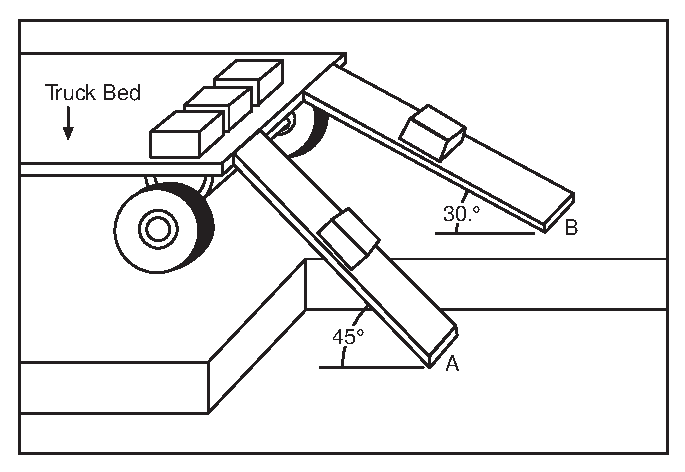
\includegraphics[keepaspectratio,scale=0.66]{Jan2001-Q17}
    \end{center}
    Compared to the amount of work done against friction by a block sliding down plank $A$,
        the work done against friction by a block sliding down plank $B$ is:
    \begin{multicols}{2}
    \begin{choices}
        \wrongchoice{less}
      \correctchoice{more}
        \wrongchoice{the same}
    \end{choices}
    \end{multicols}
\end{question}
}

\element{nysed}{
\begin{question}{Jan2001-Q18}
    Two vacationers walk out on a horizontal pier as shown in the diagram below.
    \begin{center}
        %% NOTE: very complex, keep
        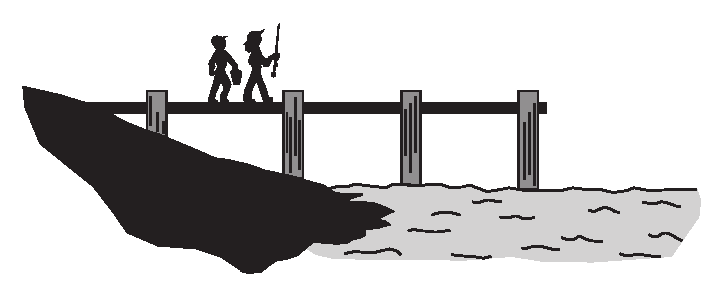
\includegraphics[keepaspectratio,scale=0.66]{Jan2001-Q18}
    \end{center}
    As they approach the end of the pier,
        their gravitational potential energy will
    \begin{multicols}{2}
    \begin{choices}
        \wrongchoice{decrease}
        \wrongchoice{increase}
      \correctchoice{remain the same}
    \end{choices}
    \end{multicols}
\end{question}
}

\element{nysed}{
\begin{question}{Jan2001-Q20}
    The graph below represents the elongation of a spring as a function of the applied force.
    \begin{center}
    \begin{tikzpicture}
        \begin{axis}[
            axis y line=left,
            axis x line=bottom,
            axis line style={->},
            xlabel={elongation},
            xtick={0,0.1,0.2,0.3,0.4},
            x unit=\si{\meter},
            ylabel={force},
            y unit=\si{\newton},
            ytick={0,6,12,18,24},
            xmin=0,xmax=0.45,
            ymin=0,ymax=27,
            grid=major,
            width=0.8\columnwidth,
            height=0.5\columnwidth,
            very thin,
        ]
        \addplot[line width=1pt,domain=0:0.41]{60*x};
        \end{axis}
    \end{tikzpicture}
    \end{center}
    How much work must be done to stretch the spring \SI{0.40}{\meter}?
    \begin{multicols}{2}
    \begin{choices}
      \correctchoice{\SI{4.8}{\joule}}
        \wrongchoice{\SI{6.0}{\joule}}
        \wrongchoice{\SI{9.8}{\joule}}
        \wrongchoice{\SI{24}{\joule}}
    \end{choices}
    \end{multicols}
\end{question}
}


%% Section June2000
%%--------------------
\element{nysed}{
\begin{question}{June2000-Q18}
    A student applies a \SI{20}{\newton} force to move a crate at a constant speed of \SI{4.0}{\meter\per\second} across a rough floor.
    How much work is done by the student on the crate in \SI{6.0}{\second}?
    \begin{multicols}{2}
    \begin{choices}
        \wrongchoice{\SI{80}{\joule}}
        \wrongchoice{\SI{120}{\joule}}
        \wrongchoice{\SI{240}{\joule}}
      \correctchoice{\SI{480}{\joule}}
    \end{choices}
    \end{multicols}
\end{question}
}

\element{nysed}{
\begin{question}{June2000-Q21}
    The kinetic energy of a \SI{980}{\kilo\gram} race car traveling at \SI{90}{\meter\per\second} is approximately:
    \begin{multicols}{2}
    \begin{choices}
        \wrongchoice{\SI{4.4e4}{\joule}}
        \wrongchoice{\SI{8.8e4}{\joule}}
      \correctchoice{\SI{4.0e6}{\joule}}
        \wrongchoice{\SI{7.9e6}{\joule}}
    \end{choices}
    \end{multicols}
\end{question}
}

\element{nysed}{
\begin{question}{June2000-Q29}
    In the diagram below, a student compressed the spring in a pop-up toy \SI{0.020}{\meter}.
    %% I changed the graph as the original did not make sense
    \begin{center}
    \begin{tikzpicture}
        \begin{axis}[
            axis y line=left,
            axis x line=bottom,
            axis line style={->},
            xlabel={compression},
            xtick=\empty,
            ylabel={force},
            ytick=\empty,
            xmin=0,xmax=10,
            ymin=0,ymax=10,
            grid=major,
            width=0.90\columnwidth,
            height=0.40\columnwidth,
            very thin,
        ]
        \addplot[line width=1pt,domain=0:10]{x};
        \end{axis}
    \end{tikzpicture}
    \end{center}
    If the spring has a spring constant of \SI{340}{\newton\per\meter},
        how much energy is being stored in the spring?
    \begin{multicols}{2}
    \begin{choices}
      \correctchoice{\SI{0.068}{\joule}}
        \wrongchoice{\SI{0.14}{\joule}}
        \wrongchoice{\SI{3.4}{\joule}}
        \wrongchoice{\SI{6.8}{\joule}}
    \end{choices}
    \end{multicols}
\end{question}
}


%% Section June1999
%%--------------------
\element{nysed}{
\begin{question}{June1999-Q19}
    A girl rides an escalator that moves her upward at constant speed.
    As the girl rises,
        how does her gravitational potential energy and kinetic energy change?
    \begin{choices}
        \wrongchoice{Gravitational potential energy decreases and kinetic energy decreases.}
        \wrongchoice{Gravitational potential energy decreases and kinetic energy remains the same.}
        \wrongchoice{Gravitational potential energy increases and kinetic energy decreases.}
      \correctchoice{Gravitational potential energy increases and kinetic energy remains the same.}
    \end{choices}
\end{question}
}

\element{nysed}{
\begin{question}{June1999-Q20}
    A student does \SI{300}{\joule} of work pushing a cart \SI{3.0}{\meter} due east and then does \SI{400}{\joule} of work pushing the cart \SI{4.0}{\meter} due north.
    The total amount of work done by the student is:
    \begin{multicols}{2}
    \begin{choices}
        \wrongchoice{\SI{100}{\joule}}
        \wrongchoice{\SI{500}{\joule}}
      \correctchoice{\SI{700}{\joule}}
        \wrongchoice{\SI{2500}{\joule}}
    \end{choices}
    \end{multicols}
\end{question}
}

\element{nysed}{
\begin{question}{June1999-Q21}
    The unstretched spring in the diagram below has a length of \SI{0.40}{\meter} and spring constant $k$.
    A weight is hung from the spring, causing it to stretch to a length of \SI{0.60}{\meter}.
    \begin{center}
    \begin{tikzpicture}
        \begin{scope}[xshift=-2cm]
            %% Title
            \node[anchor=south,text centered] at (0.5,0.2cm) {Unstretched};
            %% Celiing
            \draw (-1,0) --  (2,0);
            \node[anchor=south,fill,pattern=north east lines,minimum width=3cm, minimum height=0.05cm] at (0.5,0) {};
            %% Spring
            \draw[thick,decoration={aspect=0.2,segment length=2mm,amplitude=4mm,coil},decorate] (0,0) -- (0,-2);
            \draw[dashed]  (0,-2) -- ++(0:1cm);
            %% Ruler
            \draw[<->] (1.5,0) -- (1.5,-2) node[pos=0.5,anchor=center,fill=white] {\SI{0.40}{\meter}};
        \end{scope}
        \begin{scope}[xshift=+2cm]
            %% Title
            \node[anchor=south,text centered] at (0.5,0.2cm) {Stretched};
            %% Celiing
            \draw (-1,0) --  (2,0);
            \node[anchor=south,fill,pattern=north east lines,minimum width=3cm, minimum height=0.05cm] at (0.5,0) {};
            %% Weight
            \node[anchor=north,draw,minimum size=1cm] (M) at (0,-3) {Weight};
            %% Spring
            \draw[thick,decoration={aspect=0.2,segment length=3mm,amplitude=4mm,coil},decorate] (0,0) -- (0,-3);
            \draw[dashed]  (0,-3) -- ++(0:1cm);
            %% Ruler
            \draw[<->] (1.5,0) -- (1.5,-3) node[pos=0.5,anchor=center,fill=white] {\SI{0.60}{\meter}};
        \end{scope}
    \end{tikzpicture}
    \end{center}
    How many joules of elastic potential energy are stored in this stretched spring?
    \begin{multicols}{2}
    \begin{choices}
      \correctchoice{$0.020\times k$}
        \wrongchoice{$0.080\times k$}
        \wrongchoice{$0.18\times k$}
        \wrongchoice{$2.0\times k$}
        %% NOTE: 0.2 would be better distrator
    \end{choices}
    \end{multicols}
\end{question}
}

\element{nysed}{
\begin{question}{June1999-Q22}
    A spring has a spring constant of \SI{25}{\newton\per\meter}.
    The minimum force required to stretch the spring \SI{0.25}{\meter} from its equilibrium position is approximately:
    \begin{multicols}{2}
    \begin{choices}
        \wrongchoice{\SI{1.0e-4}{\newton}}
        \wrongchoice{\SI{0.78}{\newton}}
      \correctchoice{\SI{6.3}{\newton}}
        \wrongchoice{\SI{1.0e2}{\newton}}
    \end{choices}
    \end{multicols}
\end{question}
}

%% NOTE: June1999-Q24 requires graphics
%% NOTE: cannot extract vector graphic
%\element{nysed}{
%\begin{question}{June1999-Q24}
%    In the diagram below, an average force of \SI{20}{\newton}
%        is used to pull back the string of a bow \SI{0.60}{\meter}.
%    \begin{center}
%        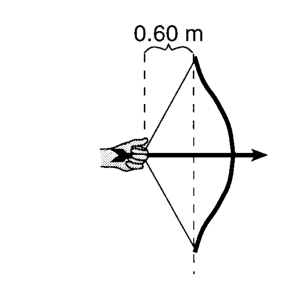
\includegraphics[keepaspectratio,scale=0.75]{June1999-Q24}
%    \end{center}
%    The arrow leaves the bow, its kinetic energy is:
%    \begin{multicols}{2}
%    \begin{choices}
%        \wrongchoice{\SI{3.4}{\joule}}
%        \wrongchoice{\SI{6.0}{\joule}}
%        \wrongchoice{\SI{12}{\joule}}
%        \wrongchoice{\SI{33}{\joule}}
%    \end{choices}
%    \end{multicols}
%\end{question}
%}


%% Section June1998
%%--------------------
\element{nysed}{
\begin{question}{June1998-Q14}
    If the speed of a moving object is doubled,
        which quantity associated with the object must also double?
    \begin{choices}
      \correctchoice{its momentum}
        \wrongchoice{its kinetic energy}
        \wrongchoice{its acceleration}
        \wrongchoice{its gravitational potential energy}
    \end{choices}
\end{question}
}

\element{nysed}{
\begin{question}{June1998-Q18}
    Which action would require no work to be done on an object?
    \begin{choices}
        \wrongchoice{lifting the object from the floor to the ceiling}
        \wrongchoice{pushing the object along a horizontal floor against a frictional force}
        \wrongchoice{decreasing the speed of the object until it comes to rest}
      \correctchoice{holding the object stationary above the ground}
    \end{choices}
\end{question}
}

\element{nysed}{
\begin{question}{June1998-Q20}
    A \SI{60}{\kilo\gram} student running at \SI{3.0}{\meter\per\second} has a kinetic energy of:
    \begin{multicols}{2}
    \begin{choices}
        \wrongchoice{\SI{180}{\joule}}
      \correctchoice{\SI{270}{\joule}}
        \wrongchoice{\SI{540}{\joule}}
        \wrongchoice{\SI{8100}{\joule}}
    \end{choices}
    \end{multicols}
\end{question}
}

\element{nysed}{
\begin{question}{June1998-Q21}
    A student pulls a box across a horizontal floor at a constant speed of \SI{4.0}{\meter\per\second} by exerting a constant horizontal force of \SI{45}{\newton}.
    Approximately how much work does the student do against friction in moving the box \SI{5.5}{\meter} across the floor?
    \begin{multicols}{2}
    \begin{choices}
        \wrongchoice{\SI{45}{\joule}}
        \wrongchoice{\SI{180}{\joule}}
      \correctchoice{\SI{250}{\joule}}
        \wrongchoice{\SI{740}{\joule}}
    \end{choices}
    \end{multicols}
\end{question}
}


%% Section June1997
%%--------------------
\element{nysed}{
\begin{question}{June1997-Q16}
    How much work is done on a downhill skier by an average braking force of \SI{9.8e2}{\newton} to stop her in a distance of \SI{10}{\meter}?
    \begin{multicols}{2}
    \begin{choices}
        \wrongchoice{\SI{1.0e1}{\joule}}
        \wrongchoice{\SI{9.8e1}{\joule}}
        \wrongchoice{\SI{1.0e3}{\joule}}
      \correctchoice{\SI{9.8e3}{\joule}}
    \end{choices}
    \end{multicols}
\end{question}
}

\element{nysed}{
\begin{question}{June1997-Q18}
    A spring has a spring constant of \SI{120}{\newton\per\meter}.
    How much potential energy is stored in the spring as it is stretched \SI{0.20}{\meter}?
    \begin{multicols}{2}
    \begin{choices}
      \correctchoice{\SI{2.4}{\joule}}
        \wrongchoice{\SI{4.8}{\joule}}
        \wrongchoice{\SI{12}{\joule}}
        \wrongchoice{\SI{24}{\joule}}
    \end{choices}
    \end{multicols}
\end{question}
}

\element{nysed}{
\begin{question}{June1997-Q21}
    A cart of mass $M$ on a frictionless track starts from rest at the top of the hill having height $h_1$,
        as shown in the diagram below.
    \begin{center}
    \begin{tikzpicture}[font=\small]
        %% Ground
        \draw[dashed] (-1,0) -- (7,0);
        %% Path
        \draw[thick] (-1,3) -- (0,3) to[out=0,in=180] (2,0) to[out=0,in=180] (4,2) to [out=0,in=180] (5.5,0.75) -- (7,0.75);
        %% Mass
        \node[draw,fill=white!90!black,minimum size=0.5cm,anchor=south] (M) at (0,3.1) {$M$};
        \draw (M.south west) ++(0:0.1) arc (90:-270:0.05);
        \draw (M.south east) ++(180:0.1) arc (90:-270:0.05);
        %% Labels
        \draw[<->] (0,0) -- (0,3) node[pos=0.5,fill=white,anchor=center] {$h_1$};
        \draw[<->] (4,0) -- (4,2) node[pos=0.5,fill=white,anchor=center] {$h_2$};
        \draw[<->] (6,0) -- (6,0.75) node[pos=0.5,anchor=west] {$h_3$};
    \end{tikzpicture}
    \end{center}
    What is the kinetic energy of the cart when it reaches the top of the next hill,
        having height $h_2$?
    \begin{multicols}{2}
    \begin{choices}
        \wrongchoice{$Mgh_1$}
      \correctchoice{$Mg\left(h_1-h_2\right)$}
        \wrongchoice{$Mg\left(h_2-h_3\right)$}
        \wrongchoice{zero}
    \end{choices}
    \end{multicols}
\end{question}
}


%% Section June1996
%%--------------------
\element{nysed}{
\begin{question}{June1996-Q18}
    A box weighing \SI{1.0e2}{\newton} is dragged to the top of an incline,
        as shown in the diagram below.
    \begin{center}
    \begin{tikzpicture}[scale=0.66,font=\small]
        %% Triangle
        \draw[thick] (0,0) -- (8,0) -- (8,6) -- cycle;
        %% Labels
        \draw[<->,thick] (0,-2em) -- (8,-2em) node[pos=0.5,anchor=center,fill=white] {\SI{8}{\meter}};
        \draw[<->,thick] (8cm+3em,0) -- (8cm+3em,6) node[pos=0.5,anchor=center,fill=white] {\SI{6}{\meter}};
        \draw[<->,thick] (126.87:2.5) -- ++(36.87:10) node[pos=0.5,anchor=center,rotate=36.87,fill=white] {\SI{10}{\meter}};
        %% block
        \node[draw,thick,minimum size=1cm,fill=white!90!black,rounded corners=0.5ex,rotate=36.87,anchor=south west] (A) at (36.87:0.01cm) {\SI{e2}{\newton}};
        \draw[thick,->] (A.east) -- ++(36.87:2);
    \end{tikzpicture}
    \end{center}
    The gravitational potential energy of the box at the top of the incline is approximately:
    \begin{multicols}{2}
    \begin{choices}
        \wrongchoice{\SI{1.0e2}{\joule}}
      \correctchoice{\SI{6.0e2}{\joule}}
        \wrongchoice{\SI{8.0e2}{\joule}}
        \wrongchoice{\SI{1.0e3}{\joule}}
    \end{choices}
    \end{multicols}
\end{question}
}

\element{nysed}{
\begin{question}{June1996-Q21}
    Spring $A$ has a spring constant of \SI{140}{\newton\per\meter},
        and spring $B$ has spring constant of \SI{280}{\newton\per\meter}.
    Both springs are stretched at the same distance.
    Compared to the potential energy stored in spring $A$,
        the potential energy stored in spring $B$ is:
    \begin{choices}
        \wrongchoice{the same}
      \correctchoice{twice as great}
        \wrongchoice{half as great}
        \wrongchoice{four times as great}
    \end{choices}
\end{question}
}

\element{nysed}{
\begin{question}{June1996-Q22}
    A cart of mass $m$ traveling at speed $v$ has kinetic energy $KE$.
    If the mass of the cart is doubled and its speed is halved,
        the kinetic energy of the cart will be:
    \begin{choices}
      \correctchoice{half as great}
        \wrongchoice{twice as great}
        \wrongchoice{one-fourth as great}
        \wrongchoice{four times as great}
    \end{choices}
\end{question}
}


%% Section June1996
%%--------------------
\element{nysed}{
\begin{question}{June1995-Q15}
    A constant force of \SI{2.0}{\newton} is used to push a \SI{3.0}{\kilo\gram} mass \SI{4.0}{\meter} across the floor.
    How much work is done on the mass?
    \begin{multicols}{2}
    \begin{choices}
        \wrongchoice{\SI{6.0}{\joule}}
      \correctchoice{\SI{8.0}{\joule}}
        \wrongchoice{\SI{12}{\joule}}
        \wrongchoice{\SI{24}{\joule}}
    \end{choices}
    \end{multicols}
\end{question}
}

\element{nysed}{
\begin{question}{June1995-Q17}
    When a spring is stretched \SI{0.200}{\meter} from its equilibrium position,
        it possesses a potential energy of \SI{10.0}{\joule}.
    What is the spring constant for this spring?
    \begin{multicols}{2}
    \begin{choices}
        \wrongchoice{\SI{100}{\newton\per\meter}}
        \wrongchoice{\SI{125}{\newton\per\meter}}
        \wrongchoice{\SI{250}{\newton\per\meter}}
      \correctchoice{\SI{500}{\newton\per\meter}}
    \end{choices}
    \end{multicols}
\end{question}
}

\element{nysed}{
\begin{question}{June1995-Q18}
    A \SI{1.0e3}{\kilo\gram} car is moving at a constant speed of \SI{4.0}{\meter\per\second}.
    What is the kinetic energy of the car?
    \begin{multicols}{2}
    \begin{choices}
        \wrongchoice{\SI{1.6e3}{\joule}}
        \wrongchoice{\SI{2.0e4}{\joule}}
      \correctchoice{\SI{8.0e3}{\joule}}
        \wrongchoice{\SI{4.0e3}{\joule}}
    \end{choices}
    \end{multicols}
\end{question}
}

\element{nysed}{
\begin{question}{June1995-Q19}
    A force is applied to a block, causing it to accelerate along a horizontal, frictionless surface.
    The energy gained by the block is equal to the:
    \begin{choices}
      \correctchoice{work done on the block}
        \wrongchoice{power applied to the block}
        \wrongchoice{impulse applied to the block}
        \wrongchoice{momentum given to the block}
    \end{choices}
\end{question}
}

\element{nysed}{
\begin{question}{June1995-Q20}
    A \SI{1.0}{\kilo\gram} mass gains kinetic energy as it falls freely from rest a vertical distance, $d$.
    How far would a \SI{2.0}{\kilo\gram} mass have to fall freely from rest to gain the same amount of kinetic energy?
    \begin{multicols}{4}
    \begin{choices}
        \wrongchoice{$d$}
        \wrongchoice{$2d$}
      \correctchoice{$\dfrac{d}{2}$}
        \wrongchoice{$\dfrac{d}{4}$}
    \end{choices}
    \end{multicols}
\end{question}
}


%% Section June1994
%%--------------------
\element{nysed}{
\begin{question}{June1994-Q19}
    Graphs $A$ and $B$ below represent the result of applying an increasing force to stretch a spring which did not exceed its elastic limit.
    \begin{center}
    \begin{tikzpicture}
        \begin{groupplot}[
                axis y line=left,
                axis x line=bottom,
                axis line style={->},
                group style={group size=2 by 1},
                xtick=\empty,
                ytick=\empty,
                xmin=0,xmax=11,
                ymin=0,ymax=11,
                ylabel={Force Applied},
                width=0.5\columnwidth,
            ]
            \nextgroupplot[
                title=$A$,
                xlabel={Spring Displacement},
            ] \addplot[line width=1pt,domain=0:10] {x};
            \nextgroupplot[
                title=$B$,
                xlabel={Work Done on Spring},
            ] \addplot[line width=1pt,domain=0:10] {sqrt(10)*sqrt(x)};
        \end{groupplot}
    \end{tikzpicture}
    \end{center}
    The spring constant can be represented by the:
    \begin{choices}
      \correctchoice{slope of graph $A$}
        \wrongchoice{slope of graph $B$}
        \wrongchoice{reciprocal of the slope of graph $A$}
        \wrongchoice{reciprocal of the slope of graph $B$}
    \end{choices}
\end{question}
}

\element{nysed}{
\begin{question}{June1994-Q20}
    A force of \SI{0.2}{\newton} is needed to compress a spring a distance of \SI{0.02}{\meter}.
    The potential energy stored in this compressed spring is:
    \begin{multicols}{2}
    \begin{choices}
        \wrongchoice{\SI{8e-5}{\joule}}
      \correctchoice{\SI{2e-3}{\joule}}
        \wrongchoice{\SI{2e-5}{\joule}}
        \wrongchoice{\SI{4e-5}{\joule}}
    \end{choices}
    \end{multicols}
\end{question}
}

\element{nysed}{
\begin{question}{June1994-Q21}
    An object with a speed of \SI{20}{\meter\per\second} has a kinetic energy of \SI{400}{\joule}.
    The mass of the object is:
    \begin{multicols}{2}
    \begin{choices}
        \wrongchoice{\SI{1.0}{\kilo\gram}}
      \correctchoice{\SI{2.0}{\kilo\gram}}
        \wrongchoice{\SI{0.50}{\kilo\gram}}
        \wrongchoice{\SI{40}{\kilo\gram}}
    \end{choices}
    \end{multicols}
\end{question}
}



%% Section June1990
%%--------------------
\element{nysed}{
\begin{question}{June1990-Q18}
    The graph below shows the force exerted on a block as a function of the block's displacement in the direction of the force.
    \begin{center}
    \begin{tikzpicture}
        \begin{axis}[
            axis y line=left,
            axis x line=bottom,
            axis line style={->},
            xlabel={displacement},
            x unit=\si{\meter},
            xtick={0,1,2,3,4,5,6,7},
            ylabel={force},
            y unit=\si{\newton},
            ytick={0,2,4,6,8},
            xmin=0,xmax=7.2,
            ymin=0,ymax=8.2,
            width=0.8\columnwidth,
            height=0.5\columnwidth,
            very thin,
        ]
        \addplot[line width=1pt,domain=0:10]{4};
        \end{axis}
    \end{tikzpicture}
    \end{center}
    How much work did the force do in displacing the block \SI{5.0}{\meter}?
    \begin{multicols}{2}
    \begin{choices}
        \wrongchoice{\SI{0}{\joule}}
      \correctchoice{\SI{20}{\joule}}
        \wrongchoice{\SI{0.80}{\joule}}
        \wrongchoice{\SI{4.0}{\joule}}
    \end{choices}
    \end{multicols}
\end{question}
}

\element{nysed}{
\begin{question}{June1990-Q20}
    When a \SI{5}{\kilo\gram} mass is lifted from ground to a height of \SI{10}{\meter},
        the gravitational potential energy of the mass is increased by approximately:
    \begin{multicols}{2}
    \begin{choices}
        \wrongchoice{\SI{0.5}{\joule}}
        \wrongchoice{\SI{2}{\joule}}
        \wrongchoice{\SI{50}{\joule}}
      \correctchoice{\SI{500}{\joule}}
    \end{choices}
    \end{multicols}
\end{question}
}

\element{nysed}{
\begin{question}{June1990-Q21}
    If the speed of an object is doubled,
        its kinetic energy will be:
    \begin{multicols}{2}
    \begin{choices}
        \wrongchoice{halved}
        \wrongchoice{doubled}
        \wrongchoice{quartered}
      \correctchoice{quadrupled}
    \end{choices}
    \end{multicols}
\end{question}
}

\element{nysed}{
\begin{question}{June1990-Q23}
    An object \SI{10}{\meter} above the ground has $Z$ joules of potential energy.
    If the object falls freely,
        how many joules of kinetic energy will it have gained when it is \SI{5}{\meter} above the ground?
    \begin{multicols}{2}
    \begin{choices}
        \wrongchoice{$Z$}
        \wrongchoice{$2Z$}
      \correctchoice{$\dfrac{Z}{2}$}
        \wrongchoice{zero}
    \end{choices}
    \end{multicols}
\end{question}
}


%% Section June1989
%%--------------------
\element{nysed}{
\begin{question}{June1989-Q23}
    An object gains \SI{10}{\joule} of potential energy as it is lifted vertically \SI{2.0}{\meter}.
    If a second object with one-half the mass is lifted vertically \SI{2.0}{\meter},
        the potential energy gained by the second object will be:
    \begin{multicols}{2}
    \begin{choices}
        \wrongchoice{\SI{10}{\joule}}
        \wrongchoice{\SI{20}{\joule}}
      \correctchoice{\SI{5.0}{\joule}}
        \wrongchoice{\SI{2.5}{\joule}}
    \end{choices}
    \end{multicols}
\end{question}
}

\element{nysed}{
\begin{question}{June1989-Q24}
    A spring of negligible mass with a spring constant of \SI{200}{\newton\per\meter} is stretched \SI{0.2}{\meter}.
    How much potential energy is stored in the spring?
    \begin{multicols}{2}
    \begin{choices}
        \wrongchoice{\SI{40}{\joule}}
        \wrongchoice{\SI{20}{\joule}}
        \wrongchoice{\SI{8}{\joule}}
      \correctchoice{\SI{4}{\joule}}
    \end{choices}
    \end{multicols}
\end{question}
}

\element{nysed}{
\begin{question}{June1989-Q25}
    Which graph best represents the relationship between the kinetic energy (KE) of a moving object as a function of its velocity?
    \begin{multicols}{2}
    \begin{choices}
        \AMCboxDimensions{down=-2.5em}
        \wrongchoice{
            \begin{tikzpicture}
                \begin{axis}[
                    axis y line=left,
                    axis x line=bottom,
                    axis line style={->},
                    xlabel={KE},
                    xtick=\empty,
                    ylabel={velocity},
                    ytick=\empty,
                    xmin=0,xmax=11,
                    ymin=0,ymax=11,
                    width=\columnwidth,
                    very thin,
                ]
                \addplot[line width=1pt,domain=0:10]{8};
                \end{axis}
            \end{tikzpicture}
        }
        \wrongchoice{
            \begin{tikzpicture}
                \begin{axis}[
                    axis y line=left,
                    axis x line=bottom,
                    axis line style={->},
                    xlabel={KE},
                    xtick=\empty,
                    ylabel={velocity},
                    ytick=\empty,
                    xmin=0,xmax=11,
                    ymin=0,ymax=11,
                    width=\columnwidth,
                    very thin,
                ]
                \addplot[line width=1pt,domain=0:10]{x};
                \end{axis}
            \end{tikzpicture}
        }
        %% ANS is 3
        \correctchoice{
            \begin{tikzpicture}
                \begin{axis}[
                    axis y line=left,
                    axis x line=bottom,
                    axis line style={->},
                    xlabel={KE},
                    xtick=\empty,
                    ylabel={velocity},
                    ytick=\empty,
                    xmin=0,xmax=11,
                    ymin=0,ymax=11,
                    width=\columnwidth,
                    very thin,
                ]
                \addplot[line width=1pt,domain=0:10]{0.1*x*x};
                \end{axis}
            \end{tikzpicture}
        }
        \wrongchoice{
            \begin{tikzpicture}
                \begin{axis}[
                    axis y line=left,
                    axis x line=bottom,
                    axis line style={->},
                    xlabel={KE},
                    xtick=\empty,
                    ylabel={velocity},
                    ytick=\empty,
                    xmin=0,xmax=11,
                    ymin=0,ymax=11,
                    width=\columnwidth,
                    very thin,
                ]
                \addplot[line width=1pt,domain=0:10]{10/x};
                \end{axis}
            \end{tikzpicture}
        }
    \end{choices}
    \end{multicols}
\end{question}
}

\element{nysed}{
\begin{question}{June1989-Q26}
    A basketball player who weighs \SI{600}{\newton} jumps \SI{0.5}{\meter} vertically off the floor.
    What is her kinetic energy just before hitting the floor?
    \begin{multicols}{2}
    \begin{choices}
        \wrongchoice{\SI{30}{\joule}}
        \wrongchoice{\SI{60}{\joule}}
      \correctchoice{\SI{300}{\joule}}
        \wrongchoice{\SI{600}{\joule}}
    \end{choices}
    \end{multicols}
\end{question}
}


%% Section June1986
%%--------------------
\element{nysed}{
\begin{question}{June1986-Q13}
    A \SI{2.2}{\kilo\gram} mass is pulled by a \SI{30}{\newton} force through a distance of \SI{5.0}{\meter} as shown in the diagram below.
    \begin{center}
    \begin{tikzpicture}
        %% ground
        \draw (-3.5,0) -- (3.5,0);
        \node[anchor=north,minimum width=7cm,pattern=north east lines] at (0,0) {};
        %% box
        \node[anchor=south,draw,minimum size=1cm] (A) at (-1,0) {\SI{2.2}{\kilo\gram}};
        \draw[thick,-latex] (A.east) -- ++(0:2) node[pos=0.5,anchor=south] {\SI{30}{\newton}};
        %% distance
        \draw[dashed] (A.north east) -- ++(90:1);
        \draw[<->] (A.north east) ++(90:0.75) -- ++(0:3) node[pos=0.5,anchor=center,fill=white] {\SI{50}{\meter}};
        \draw[dashed] (A.north east) ++ (90:1) ++ (0:3) -- ++(270:1);
    \end{tikzpicture}
    \end{center}
    What amount of work is done?
    \begin{multicols}{2}
    \begin{choices}
        \wrongchoice{\SI{11}{\joule}}
        \wrongchoice{\SI{66}{\joule}}
      \correctchoice{\SI{150}{\joule}}
        \wrongchoice{\SI{330}{\joule}}
    \end{choices}
    \end{multicols}
\end{question}
}

\element{nysed}{
\begin{question}{June1986-Q14}
    A mass resting on a shelf \SI{10.0}{\meter} above the floor has a gravitational potential energy of \SI{980}{\joule} with respect to the floor.
    The mass is moved to a shelf \SI{8.00}{\meter} above the floor.
    What is the new gravitational potential energy?
    \begin{multicols}{2}
    \begin{choices}
        \wrongchoice{\SI{960}{\joule}}
      \correctchoice{\SI{784}{\joule}}
        \wrongchoice{\SI{490}{\joule}}
        \wrongchoice{\SI{196}{\joule}}
    \end{choices}
    \end{multicols}
\end{question}
}

\element{nysed}{
\begin{question}{June1986-Q16}
    Which cart shown below has the greatest kinetic energy?
    \begin{multicols}{2}
    \begin{choices}
        \AMCboxDimensions{down=-0.4cm}
        %% NOTE: ANS is 2
        \wrongchoice{
            \begin{tikzpicture}
                \draw[dashed,white!60!black] (-1.5,-0.5) rectangle (1.5,2.5);
                %% ground
                \draw (-1.5,0) -- (1.5,0);
                \node[anchor=north,minimum width=3cm,pattern=north east lines] at (0,0) {};
                %% Cart
                \node[draw,minimum height=1.0cm,minimum width=2.0cm,anchor=south] (L) at (0,0.2) {\SI{1}{\kilo\gram}};
                \draw[fill=white] (L.south west) ++(0:0.3) circle (0.2);
                \draw[fill=black] (L.south west) ++(0:0.3) circle (1pt);
                \draw[fill=white] (L.south east) ++(180:0.3) circle (0.2);
                \draw[fill=black] (L.south east) ++(180:0.3) circle (1pt);
                \draw[thick,->] (L.north west) ++(90:1em) -- ++(0:2cm) node[pos=0.5,anchor=south] {\SI{4}{\meter\per\second}};
            \end{tikzpicture}
        }
        \wrongchoice{
            \begin{tikzpicture}
                \draw[dashed,white!60!black] (-1.5,-0.5) rectangle (1.5,2.5);
                %% ground
                \draw (-1.5,0) -- (1.5,0);
                \node[anchor=north,minimum width=3cm,pattern=north east lines] at (0,0) {};
                %% Cart
                \node[draw,minimum height=1.0cm,minimum width=2.0cm,anchor=south] (L) at (0,0.2) {\SI{2}{\kilo\gram}};
                \draw[fill=white] (L.south west) ++(0:0.3) circle (0.2);
                \draw[fill=black] (L.south west) ++(0:0.3) circle (1pt);
                \draw[fill=white] (L.south east) ++(180:0.3) circle (0.2);
                \draw[fill=black] (L.south east) ++(180:0.3) circle (1pt);
                \draw[thick,->] (L.north west) ++(90:1em) -- ++(0:2cm) node[pos=0.5,anchor=south] {\SI{3}{\meter\per\second}};
            \end{tikzpicture}
        }
        \wrongchoice{
            \begin{tikzpicture}
                \draw[dashed,white!60!black] (-1.5,-0.5) rectangle (1.5,2.5);
                %% ground
                \draw (-1.5,0) -- (1.5,0);
                \node[anchor=north,minimum width=3cm,pattern=north east lines] at (0,0) {};
                %% Cart
                \node[draw,minimum height=1.0cm,minimum width=2.0cm,anchor=south] (L) at (0,0.2) {\SI{3}{\kilo\gram}};
                \draw[fill=white] (L.south west) ++(0:0.3) circle (0.2);
                \draw[fill=black] (L.south west) ++(0:0.3) circle (1pt);
                \draw[fill=white] (L.south east) ++(180:0.3) circle (0.2);
                \draw[fill=black] (L.south east) ++(180:0.3) circle (1pt);
                \draw[thick,->] (L.north east) ++(90:1em) -- ++(180:2cm) node[pos=0.5,anchor=south] {\SI{2}{\meter\per\second}};
            \end{tikzpicture}
        }
        \wrongchoice{
            \begin{tikzpicture}
                \draw[dashed,white!60!black] (-1.5,-0.5) rectangle (1.5,2.5);
                %% ground
                \draw (-1.5,0) -- (1.5,0);
                \node[anchor=north,minimum width=3cm,pattern=north east lines] at (0,0) {};
                %% Cart
                \node[draw,minimum height=1.0cm,minimum width=2.0cm,anchor=south] (L) at (0,0.2) {\SI{4}{\kilo\gram}};
                \draw[fill=white] (L.south west) ++(0:0.3) circle (0.2);
                \draw[fill=black] (L.south west) ++(0:0.3) circle (1pt);
                \draw[fill=white] (L.south east) ++(180:0.3) circle (0.2);
                \draw[fill=black] (L.south east) ++(180:0.3) circle (1pt);
                \draw[thick,->] (L.north east) ++(90:1em) -- ++(180:2cm) node[pos=0.5,anchor=south] {\SI{1}{\meter\per\second}};
            \end{tikzpicture}
        }
    \end{choices}
    \end{multicols}
\end{question}
}


%% Section June1985
%%--------------------
\element{nysed}{
\begin{question}{June1985-Q11}
    A \SI{1.0}{\kilo\gram} mass falls a distance of \SI{0.50}{\meter},
        causing a \SI{2.0}{\kilo\gram} mass to slide the same distance along a table top,
        as represented in the diagram below.
    \begin{center}
    \begin{tikzpicture}
        %% Floor
        \draw[thick] (-4,0) -- (0,0) -- (0,-2);
        \node[anchor=north,minimum width=4cm,pattern=north east lines] at (-2,0) {};
        %% Mass
        \node[draw,fill=white!90!black,rectangle,rounded corners=1ex,minimum size=1.22cm,anchor=south] (A) at (-3,0) {\SI{2.0}{\kilo\gram}};
        \node[draw,fill=white!90!black,rectangle,rounded corners=1ex,minimum size=1.00cm,anchor=north] (B) at (1,-0.5) {\SI{1.0}{\kilo\gram}};
        %% Rope and Pulley
        \draw[thick] (A.south east) ++(90:0.5) -- (0.75,0.5) arc(90:0:0.25) -- (B.north);
        \draw[thick,fill=white!90!black] (0.75,0.25) circle (0.25);
        \draw[thick,fill=white] (0,0) -- (0.75,0.35) arc (90:-60:0.1) -- (0,-0.5) -- cycle;
        \draw[fill] (0.75,0.25) circle (1pt);
        %% distance
        \draw[<->] (B.south) -- ++(270:2) node[pos=0.5,anchor=center,fill=white] {\SI{0.50}{\meter}};
        \draw (B.south) ++ (270:2) -- ++(0:1) -- ++(180:2);
        \path (B.south) ++ (270:2) node[anchor=north,minimum width=2cm,pattern=north east lines] {};
    \end{tikzpicture}
    \end{center}
    How much work is done by the falling mass?
    \begin{multicols}{2}
    \begin{choices}
        \wrongchoice{\SI{1.5}{\joule}}
      \correctchoice{\SI{4.9}{\joule}}
        \wrongchoice{\SI{9.8}{\joule}}
        \wrongchoice{\SI{14.7}{\joule}}
    \end{choices}
    \end{multicols}
\end{question}
}

\element{nysed}{
\begin{question}{June1985-Q12}
    Which quantities are measured in the same units?
    \begin{multicols}{2}
    \begin{choices}
        \wrongchoice{mass and weight}
        \wrongchoice{heat and temperature}
        \wrongchoice{power and work}
      \correctchoice{work and energy}
    \end{choices}
    \end{multicols}
\end{question}
}

\element{nysed}{
\begin{question}{June1985-Q13}
    The diagram below represents a cart traveling from left to right along a frictionless surface with an initial speed of $v$.
    \begin{center}
    \begin{tikzpicture}[font=\small]
        %% Path
        \draw[very thick] (-4,3) -- (-2,3) to[out=0,in=180] (0,1) to[out=0,in=180] (2,2) -- (4,2);
        \node[anchor=south east] at (4,2) {Earth's Surface};
        %% Cart
        \node[draw,fill=white!90!black,minimum width=1.25cm,minimum height=0.75cm,anchor=south] (M) at (-3,3.2) {};
        \draw[fill=white] (M.south west) ++(+0.3,0) circle (0.2);
        \draw[fill=black] (M.south west) ++(+0.3,0) circle (1pt);
        \draw[fill=white] (M.south east) ++(-0.3,0) circle (0.2);
        \draw[fill=black] (M.south east) ++(-0.3,0) circle (1pt);
        \draw[thick,-latex] (M.north west) ++(90:2ex) -- ++(0:1.25cm) node[pos=0.5,anchor=south] {$v$};
        %% Labels
        \fill (-2,3) circle (2pt) node[anchor=north] {$A$};
        \fill (0,1) circle (2pt) node[anchor=north] {$B$};
        \fill (1,1.5) circle (2pt) node[anchor=north west] {$C$};
        \fill (2,2) circle (2pt) node[anchor=north] {$D$};
    \end{tikzpicture}
    \end{center}
    At which point is the gravitational potential energy of the car \emph{least}?
    \begin{multicols}{4}
    \begin{choices}[o]
        \wrongchoice{$A$}
      \correctchoice{$B$}
        \wrongchoice{$C$}
        \wrongchoice{$D$}
    \end{choices}
    \end{multicols}
\end{question}
}

\element{nysed}{
\begin{question}{June1985-Q14}
    If the velocity of an automobile is doubled,
        its kinetic energy:
    \begin{choices}
        \wrongchoice{decrease to one-half}
        \wrongchoice{doubles}
        \wrongchoice{decrease to one-fourth}
      \correctchoice{quadruples}
    \end{choices}
\end{question}
}

\element{nysed}{
\begin{question}{June1985-Q57}
    As an object falls freely in a vacuum,
        its total energy:
    \begin{choices}
        \wrongchoice{decreases}
        \wrongchoice{increases}
      \correctchoice{remains the same}
    \end{choices}
\end{question}
}


\endinput



%
%% Power Questions used on the
%% NYSED Physics Regents Examination
%%--------------------------------------------------

%% this section contains 42 problems


%% Section June2016
%%--------------------
\element{nysed}{
\begin{question}{June2016-Q01}
	Which quantity is a vector?
    \begin{multicols}{2}
    \begin{choices}
        \wrongchoice{power}
        \wrongchoice{kinetic energy}
        \wrongchoice{speed}
      \correctchoice{weight}
    \end{choices}
    \end{multicols}
\end{question}
}

\element{nysed}{
\begin{question}{June2016-Q17}
    A motor does a total of \SI{480}{\joule} of work in \SI{5.0}{\second} to lift a \SI{12}{\kilo\gram} block to the top of a ramp. 
    The average power developed by the motor is:
    \begin{multicols}{2}
    \begin{choices}
        \wrongchoice{\SI{8.0}{\watt}}
        \wrongchoice{\SI{40.}{\watt}}
      \correctchoice{\SI{96}{\watt}}
        \wrongchoice{\SI{2400}{\watt}}
    \end{choices}
    \end{multicols}
\end{question}
}

\element{nysed}{
\begin{question}{June2016-Q18}
    A \SI{5.8e4}{\watt} elevator motor can lift a total weight of \SI{2.1e4}{\newton} with a maximum constant speed of:
    \begin{multicols}{2}
    \begin{choices}
        \wrongchoice{\SI{0.28}{\meter\per\second}}
        \wrongchoice{\SI{0.36}{\meter\per\second}}
      \correctchoice{\SI{2.8}{\meter\per\second}}
        \wrongchoice{\SI{3.6}{\meter\per\second}}
    \end{choices}
    \end{multicols}
\end{question}
}


%% Section June2015
%%--------------------
\element{nysed}{
\begin{question}{June2015-Q44}
    An electric motor has a rating of \SI{4.0e2}{\watt}.
    How much time will it take for this motor to lift a \SI{50}{\kilo\gram} mass a vertical distance of \SI{8.0}{\meter}?
    [Assume \SI{100}{\percent} efficiency.]
    \begin{multicols}{2}
    \begin{choices}
        \wrongchoice{\SI{0.98}{\second}}
        \wrongchoice{\SI{9.8}{\second}}
      \correctchoice{\SI{98}{\second}}
        \wrongchoice{\SI{980}{\second}}
    \end{choices}
    \end{multicols}
\end{question}
}


%% Section June2014
%%--------------------
\element{nysed}{
\begin{question}{June2014-Q50}
    The graph below represents the work done against gravity by a student as she walks up a flight of stairs at constant speed.
    \begin{center}
    \begin{tikzpicture}
        \begin{axis}[
            axis y line=left,
            axis x line=bottom,
            axis line style={->},
            xlabel={time},
            x unit=\si{\second},
            xtick={0,1,2,3,4,5,6,7},
            ylabel={work},
            y unit=\si{\joule},
            ytick={0,400,800,1200,1600},
            xmin=0,xmax=7.2,
            ymin=0,ymax=1650,
            grid=major,
            width=0.8\columnwidth,
            height=0.5\columnwidth,
            very thin,
        ]
        \addplot[line width=1pt,domain=0:7]{800*x/3};
        \end{axis}
    \end{tikzpicture}
    \end{center}
    Compared to the power generated by the student after \SI{2.0}{\second} the power generated by the student after \SI{4.0}{\second} is:
    \begin{choices}
      \correctchoice{twice as great}
        \wrongchoice{the same}
        \wrongchoice{half as great}
        \wrongchoice{four times as great}
    \end{choices}
\end{question}
}


%% Section June2013
%%--------------------
\element{nysed}{
\begin{question}{June2013-Q39}
    If a motor lifts a \SI{400}{\kilo\gram} mass a vertical distance of \SI{10}{\meter} in \SI{8.0}{\second},
        the \emph{minimum} power generated by the motor is:
    \begin{multicols}{2}
    \begin{choices}
        \wrongchoice{\SI{3.2e2}{\watt}}
        \wrongchoice{\SI{5.0e2}{\watt}}
      \correctchoice{\SI{4.9e3}{\watt}}
        \wrongchoice{\SI{3.2e4}{\watt}}
    \end{choices}
    \end{multicols}
\end{question}
}


%% Section June2012
%%--------------------
\element{nysed}{
\begin{question}{June2012-Q22}
    The Watt second (\si{\watt\second}) is a unit of:
    \begin{choices}
        \wrongchoice{power}
      \correctchoice{energy}
        \wrongchoice{potential difference}
        \wrongchoice{electric field strength}
    \end{choices}
\end{question}
}

\element{nysed}{
\begin{question}{June2012-Q23}
    Which quantity has both a magnitude and a direction?
    \begin{multicols}{2}
    \begin{choices}
        \wrongchoice{energy}
      \correctchoice{impulse}
        \wrongchoice{power}
        \wrongchoice{work}
    \end{choices}
    \end{multicols}
\end{question}
}

\element{nysed}{
\begin{question}{June2012-Q39}
    Two elevators, $A$ and $B$, move at constant speed.
    Elevator $B$ moves with twice the speed of elevator $A$.
    Elevator $B$ weighs twice as much as elevator $A$.
    Compared to the power needed to lift elevator $A$,
        the power needed to lift elevator $B$ is:
    \begin{choices}
        \wrongchoice{the same}
        \wrongchoice{twice as great}
        \wrongchoice{half as great}
      \correctchoice{four times as great}
    \end{choices}
\end{question}
}

\element{nysed}{
\begin{question}{June2012-Q40}
    What is the maximum height to which a motor having a power rating of \SI{20.4}{\watt} can lift a \SI{5.00}{\kilo\gram} stone vertically in \SI{10.0}{\second}?
    \begin{multicols}{2}
    \begin{choices}
        \wrongchoice{\SI{0.0416}{\meter}}
        \wrongchoice{\SI{0.408}{\meter}}
      \correctchoice{\SI{4.16}{\meter}}
        \wrongchoice{\SI{40.8}{\meter}}
    \end{choices}
    \end{multicols}
\end{question}
}


%% Section June2011
%%--------------------
\element{nysed}{
\begin{question}{June2011-Q10}
    What is the power output of an electric motor that lifts a \SI{2.0}{\kilo\gram} block \SI{15}{\meter} vertically in \SI{6.0}{\second}?
    \begin{multicols}{2}
    \begin{choices}
        \wrongchoice{\SI{5.0}{\joule}}
        \wrongchoice{\SI{5.0}{\watt}}
        \wrongchoice{\SI{49}{\joule}}
      \correctchoice{\SI{49}{\watt}}
    \end{choices}
    \end{multicols}
\end{question}
}


%% Section June2010
%%--------------------
\element{nysed}{
\begin{question}{June2010-Q38}
    A small electric motor is used to lift a \SI{0.50}{\kilo\gram} mass at constant speed.
    If the mass is lifted a vertical distance of \SI{1.5}{\meter} in \SI{5.0}{\second},
        the average power developed by the motor is:
    \begin{multicols}{2}
    \begin{choices}
        \wrongchoice{\SI{0.15}{\watt}}
      \correctchoice{\SI{1.5}{\watt}}
        \wrongchoice{\SI{3.8}{\watt}}
        \wrongchoice{\SI{7.5}{\watt}}
    \end{choices}
    \end{multicols}
\end{question}
}


%% Section June2009
%%--------------------
\element{nysed}{
\begin{question}{June2009-Q13}
    A \SI{70}{\kilo\gram} cyclist develops \SI{210}{\watt} of power while pedaling at a constant velocity of \SI{7.0}{\meter\per\second} east.
    What average force is exerted eastward on the bicycle to maintain this constant speed?
    \begin{multicols}{2}
    \begin{choices}
        \wrongchoice{\SI{490}{\newton}}
      \correctchoice{\SI{30}{\newton}}
        \wrongchoice{\SI{3.0}{\newton}}
        \wrongchoice{\SI{0}{\newton}}
    \end{choices}
    \end{multicols}
\end{question}
}


%% Section Jan2009
%%--------------------
\element{nysed}{
\begin{question}{Jan2009-Q09}
    What is the average power required to raise a \SI{1.81e4}{\newton} elevator \SI{12.0}{\meter} in \SI{22.5}{\second}?
    \begin{multicols}{2}
    \begin{choices}
        \wrongchoice{\SI{8.04e2}{\watt}}
      \correctchoice{\SI{9.65e3}{\watt}}
        \wrongchoice{\SI{2.17e5}{\watt}}
        \wrongchoice{\SI{4.89e6}{\watt}}
    \end{choices}
    \end{multicols}
\end{question}
}


%% Section June2008
%%--------------------
\element{nysed}{
\begin{question}{June2008-Q17}
    A \SI{60}{\kilo\gram} student climbs a ladder a vertical distance of \SI{4.0}{\meter} in \SI{8.0}{\second}.
    Approximately how much total work is done against gravity by the student during the climb?
    \begin{multicols}{2}
    \begin{choices}
      \correctchoice{\SI{2.4e3}{\joule}}
        \wrongchoice{\SI{2.9e2}{\joule}}
        \wrongchoice{\SI{2.4e2}{\joule}}
        \wrongchoice{\SI{3.0e1}{\joule}}
    \end{choices}
    \end{multicols}
\end{question}
}

\element{nysed}{
\begin{question}{June2008-Q19}
    What is the maximum amount of work that a \SI{6000}{\watt} motor can do in \SI{10}{\second}?
    \begin{multicols}{2}
    \begin{choices}
        \wrongchoice{\SI{6.0e1}{\joule}}
        \wrongchoice{\SI{6.0e2}{\joule}}
        \wrongchoice{\SI{6.0e3}{\joule}}
      \correctchoice{\SI{6.0e4}{\joule}}
    \end{choices}
    \end{multicols}
\end{question}
}


%% Section Jan2008
%%--------------------
\element{nysed}{
\begin{question}{Jan2008-Q14}
    Student $A$ lifts a \SI{50}{\newton} box from the floor to a height of \SI{0.40}{\meter} in \SI{2.0}{\second}.
    Student $B$ lifts a \SI{40}{\newton} box from the floor to a height of \SI{0.5}{\meter} in \SI{1.0}{\second}.
    Compared to student $A$, student $B$ does:
    \begin{choices}
        \wrongchoice{the same work but develops more power}
      \correctchoice{the same work but develops less power}
        \wrongchoice{more work but develops less power}
        \wrongchoice{less work but develops more power}
    \end{choices}
\end{question}
}


%% Section June2007
%%--------------------
\element{nysed}{
\begin{question}{June2007-Q13}
    Which quantity is a measure of the rate at which work is done?
    \begin{multicols}{2}
    \begin{choices}
      \correctchoice{power}
        \wrongchoice{momentum}
        \wrongchoice{velocity}
        \wrongchoice{energy}
    \end{choices}
    \end{multicols}
\end{question}
}

\element{nysed}{
\begin{question}{June2007-Q44}
    Which graph best represents the relationship between the power required to raise an elevator and the speed at which the elevator rises?
    \begin{multicols}{2}
    \begin{choices}
        \AMCboxDimensions{down=-2.5em}
        \correctchoice{
            \begin{tikzpicture}
                \begin{axis}[
                    axis y line=left,
                    axis x line=bottom,
                    axis line style={->},
                    xlabel={speed},
                    xtick=\empty,
                    ylabel={power},
                    ytick=\empty,
                    xmin=0,xmax=11,
                    ymin=0,ymax=11,
                    width=0.95\columnwidth,
                    height=\columnwidth,
                    very thin,
                ]
                \addplot[line width=1pt,domain=0:10]{x};
                \end{axis}
            \end{tikzpicture}
        }
        \wrongchoice{
            \begin{tikzpicture}
                \begin{axis}[
                    axis y line=left,
                    axis x line=bottom,
                    axis line style={->},
                    xlabel={speed},
                    xtick=\empty,
                    ylabel={power},
                    ytick=\empty,
                    xmin=0,xmax=11,
                    ymin=0,ymax=11,
                    width=0.95\columnwidth,
                    height=\columnwidth,
                    very thin,
                ]
                \addplot[line width=1pt,domain=0:10]{10/x};
                \end{axis}
            \end{tikzpicture}
        }
        \wrongchoice{
            \begin{tikzpicture}
                \begin{axis}[
                    axis y line=left,
                    axis x line=bottom,
                    axis line style={->},
                    xlabel={speed},
                    xtick=\empty,
                    ylabel={power},
                    ytick=\empty,
                    xmin=0,xmax=11,
                    ymin=0,ymax=11,
                    width=0.95\columnwidth,
                    height=\columnwidth,
                    very thin,
                ]
                \addplot[line width=1pt,domain=0:10]{8};
                \end{axis}
            \end{tikzpicture}
        }
        \wrongchoice{
            \begin{tikzpicture}
                \begin{axis}[
                    axis y line=left,
                    axis x line=bottom,
                    axis line style={->},
                    xlabel={speed},
                    xtick=\empty,
                    ylabel={power},
                    ytick=\empty,
                    xmin=0,xmax=11,
                    ymin=0,ymax=11,
                    width=0.95\columnwidth,
                    height=\columnwidth,
                    very thin,
                ]
                \addplot[line width=1pt,domain=0:10]{10-x};
                \end{axis}
            \end{tikzpicture}
        }
    \end{choices}
    \end{multicols}
\end{question}
}


%% Section Jan2007
%%--------------------
\element{nysed}{
\begin{question}{Jan2007-Q46}
    A \SI{110}{\kilo\gram} bodybuilder and his \SI{55}{\kilo\gram} friend run up identical flights of stairs.
    The body building reaches the top in \SI{4.0}{\second} while his friend takes \SI{2.0}{\second}.
    Compared to the power developed by the bodybuilder while running up the stairs,
        the power developed by his friend is:
    \begin{choices}
      \correctchoice{the same}
        \wrongchoice{twice as much}
        \wrongchoice{four times as much}
        \wrongchoice{half as much}
    \end{choices}
\end{question}
}


%% Section June2006
%%--------------------


%% Section Jan2006
%%--------------------
\element{nysed}{
\begin{question}{Jan2006-Q21}
    A truck weighing \SI{3.0e4}{\newton} was driven up a hill that is \SI{1.6e3}{\meter} long to a level area that is \SI{8.0e2}{\meter} above the starting point.
    If the trip took \SI{480}{\second},
        what was the \emph{minimum} power required?
    \begin{multicols}{2}
    \begin{choices}
      \correctchoice{\SI{5.0e4}{\watt}}
        \wrongchoice{\SI{1.0e5}{\watt}}
        \wrongchoice{\SI{1.2e10}{\watt}}
        \wrongchoice{\SI{2.3e10}{\watt}}
    \end{choices}
    \end{multicols}
\end{question}
}

\element{nysed}{
\begin{question}{Jan2006-Q37}
    Which pair of quantities can be expressed using the same units:
    \begin{choices}
      \correctchoice{work and kinetic energy}
        \wrongchoice{power and momentum}
        \wrongchoice{impulse and potential energy}
        \wrongchoice{acceleration and weight}
    \end{choices}
\end{question}
}


%% Section June2005
%%--------------------
\element{nysed}{
\begin{question}{June2005-Q18}
    A \SI{95}{\kilo\gram} student climbs \SI{4.0}{\meter} up a rope in \SI{3.0}{\second}.
    What is the power output of the student?
    \begin{multicols}{2}
    \begin{choices}
      \correctchoice{\SI{1.2e3}{\watt}}
        \wrongchoice{\SI{3.7e3}{\watt}}
        \wrongchoice{\SI{1.3e2}{\watt}}
        \wrongchoice{\SI{3.8e2}{\watt}}
    \end{choices}
    \end{multicols}
\end{question}
}


%% Section Jan2005
%%--------------------
\element{nysed}{
\begin{question}{Jan2005-Q24}
    A motor used \SI{120}{\watt} of power to raise a \SI{15}{\newton} object in \SI{4.0}{\second}.
    Through what vertical distance was the object raised?
    \begin{multicols}{2}
    \begin{choices}
      \correctchoice{\SI{40}{\meter}}
        \wrongchoice{\SI{1.6}{\meter}}
        \wrongchoice{\SI{8.0}{\meter}}
        \wrongchoice{\SI{360}{\meter}}
    \end{choices}
    \end{multicols}
\end{question}
}

\element{nysed}{
\begin{question}{Jan2005-Q39}
    Which unit is equivalent to a newton per kilogram (\si{\newton\per\kilo\gram})?
    \begin{choices}
      \correctchoice{meter per second squared (\si{\meter\per\second\squared})}
        \wrongchoice{watt per meter (\si{\watt\per\meter})}
        \wrongchoice{joule second (\si{\joule\second})}
        \wrongchoice{kilogram meter per second (\si{\kilo\gram\meter\per\second})}
    \end{choices}
\end{question}
}


%% Section June2004
%%--------------------
\element{nysed}{
\begin{question}{June2004-Q15}
    A \SI{40}{\newton} student runs up a staircase to a floor that is \SI{5.0}{\meter} higher than her starting point in \SI{7.0}{\second}.
    The students power output is:
    \begin{multicols}{2}
    \begin{choices}
      \correctchoice{\SI{280}{\watt}}
        \wrongchoice{\SI{1.4e3}{\watt}}
        \wrongchoice{\SI{1.4e4}{\watt}}
        \wrongchoice{\SI{29}{\watt}}
    \end{choices}
    \end{multicols}
\end{question}
}


%% Section Jan2004
%%--------------------
\element{nysed}{
\begin{question}{Jan2004-Q19}
    A boat weighing \SI{9.0e2}{\newton} requires a horizontal force of \SI{6.0e2}{\newton} to move it across the water at \SI{1.5e1}{\meter\per\second}.
    The boat's engine must provide energy at the rate of:
    \begin{multicols}{2}
    \begin{choices}
      \correctchoice{\SI{9.0e3}{\watt}}
        \wrongchoice{\SI{4.0e1}{\watt}}
        \wrongchoice{\SI{2.5e-2}{\joule}}
        \wrongchoice{\SI{7.5e3}{\joule}}
    \end{choices}
    \end{multicols}
\end{question}
}

\element{nysed}{
\begin{question}{Jan2004-Q40}
    The graph below represents the relationship between work done by a student running up a flight and the time of ascent.
    \begin{center}
    \begin{tikzpicture}
        \begin{axis}[
            axis y line=left,
            axis x line=bottom,
            axis line style={->},
            xlabel={time},
            x unit=\si{\second},
            xtick=\empty,
            ylabel={work},
            y unit=\si{\joule},
            ytick=\empty,
            xmin=0,xmax=10,
            ymin=0,ymax=10,
            grid=major,
            width=0.8\columnwidth,
            height=0.5\columnwidth,
            very thin,
        ]
        \addplot[line width=1pt,domain=0:10]{x};
        \end{axis}
    \end{tikzpicture}
    \end{center}
    What does the slope of this graph represent?
    \begin{multicols}{2}
    \begin{choices}
      \correctchoice{power}
        \wrongchoice{impulse}
        \wrongchoice{speed}
        \wrongchoice{momentum}
    \end{choices}
    \end{multicols}
\end{question}
}


%% Section June2003
%%--------------------
\element{nysed}{
\begin{question}{June2003-Q20}
    What is the average power developed by a motor as it lifts a \SI{400}{\kilo\gram} mass at constant speed through a vertical distance of \SI{10.0}{\meter} in \SI{8.0}{\second}?
    \begin{multicols}{2}
    \begin{choices}
      \correctchoice{\SI{4900}{\watt}}
        \wrongchoice{\SI{32000}{\watt}}
        \wrongchoice{\SI{320}{\watt}}
        \wrongchoice{\SI{500}{\watt}}
    \end{choices}
    \end{multicols}
\end{question}
}

\element{nysed}{
\begin{question}{June2003-Q40}
    The graph below shows the relationship between the work done by a student and the time of ascent as the student runs up a flight of stairs.
    \begin{center}
    \begin{tikzpicture}
        \begin{axis}[
            axis y line=left,
            axis x line=bottom,
            axis line style={->},
            xlabel={time},
            x unit=\si{\second},
            xtick=\empty,
            ylabel={work},
            y unit=\si{\joule},
            ytick=\empty,
            xmin=0,xmax=10,
            ymin=0,ymax=10,
            grid=major,
            width=0.8\columnwidth,
            height=0.5\columnwidth,
            very thin,
        ]
        \addplot[line width=1pt,domain=0:10]{x};
        \end{axis}
    \end{tikzpicture}
    \end{center}
    The slope of the graph would have units of:
    \begin{multicols}{2}
    \begin{choices}
      \correctchoice{watts}
        \wrongchoice{joules}
        \wrongchoice{seconds}
        \wrongchoice{newtons}
    \end{choices}
    \end{multicols}
\end{question}
}


%% Section Jan2003
%%--------------------
\element{nysed}{
\begin{question}{Jan2003-Q18}
    A \SI{3.0}{\kilo\gram} block is initially at rest on a frictionless, horizontal surface.
    The block is moved \SI{8.0}{\meter} in \SI{2.0}{\second} by the application of a \SI{12}{\newton} horizontal force,
        as shown in the diagram below.
    \begin{center}
    \begin{tikzpicture}[font=\small]
        %% Frictionless surface
        \draw (-4,0) -- (4,0);
        \node[anchor=north,fill,pattern=north east lines,minimum width=8cm, minimum height=0.01cm] at (0,0) {};
        \node[text centered,anchor=north] at (0,-0.25) {Frictionless Surface}; 
        %% 3 kg block
        \node[draw,anchor=south,fill=white!90!black,minimum size=1cm] (A) at (-3.25,0) {\SI{3.0}{\kilo\gram}};
        \draw[thick,->] (A.east) -- ++(0:2) node[pos=0.5,anchor=south] {\SI{12}{\newton}};
        %% distance
        \draw[thick,<->] (-2.75,1.5) -- (4,1.5) node[pos=0.5,anchor=center,fill=white] {\SI{8.0}{\meter}};
        \draw (-2.75,1.25) -- (-2.75,1.75);
        \draw (4,1.25) -- (4,1.75);
    \end{tikzpicture}
    \end{center}
    What is the average power developed while moving the block?
    \begin{multicols}{2}
    \begin{choices}
      \correctchoice{\SI{48}{\watt}}
        \wrongchoice{\SI{96}{\watt}}
        \wrongchoice{\SI{24}{\watt}}
        \wrongchoice{\SI{32}{\watt}}
    \end{choices}
    \end{multicols}
\end{question}
}

\element{nysed}{
\begin{question}{Jan2003-Q35}
    One watt (\si{\watt}) is equivalent to one:
    \begin{choices}
      \correctchoice{joule per second (\si{\joule\per\second})}
        \wrongchoice{joule second (\si{\joule\second})}
        \wrongchoice{newton per meter (\si{\newton\per\meter})}
        \wrongchoice{newton meter (\si{\newton\meter})}
    \end{choices}
\end{question}
}


%% Section Aug2002
%%--------------------
\element{nysed}{
\begin{question}{Aug2002-Q29}
    In raising an object vertically at a constant speed of \SI{2.0}{\meter\per\second},
        \SI{10}{\watt} of power is developed.
    %% altered wording
    The weight of the object is one watt is equivalent to:
    \begin{multicols}{2}
    \begin{choices}
      \correctchoice{\SI{5.0}{\newton}}
        \wrongchoice{\SI{20}{\newton}}
        \wrongchoice{\SI{40}{\newton}}
        \wrongchoice{\SI{50}{\newton}}
    \end{choices}
    \end{multicols}
\end{question}
}


%% Section June2002
%%--------------------
\element{nysed}{
\begin{question}{June2002-Q01}
    Which is a vector quantity?
    \begin{multicols}{2}
    \begin{choices}
        \wrongchoice{distance}
        \wrongchoice{speed}
        \wrongchoice{power}
      \correctchoice{force}
    \end{choices}
    \end{multicols}
\end{question}
}

\element{nysed}{
\begin{question}{June2002-Q32}
    What is the maximum height to which a \SI{1200}{\watt} motor could lift an object weighing \SI{200}{\newton} in \SI{4.0}{\second}?
    \begin{multicols}{2}
    \begin{choices}
        \wrongchoice{\SI{0.67}{\meter}}
        \wrongchoice{\SI{1.5}{\meter}}
        \wrongchoice{\SI{6.0}{\meter}}
      \correctchoice{\SI{24}{\meter}}
    \end{choices}
    \end{multicols}
\end{question}
}


%% Section Jan2002
%%--------------------
\element{nysed}{
\begin{question}{Jan2002-Q23}
    A \SI{10}{\newton} force is required to move a \SI{3.0}{\kilo\gram} box at constant speed.
    How much power is required to move the box \SI{8.0}{\meter} in \SI{2.0}{\second}?
    \begin{multicols}{2}
    \begin{choices}
      \correctchoice{\SI{40}{\watt}}
        \wrongchoice{\SI{20}{\watt}}
        \wrongchoice{\SI{15}{\watt}}
        \wrongchoice{\SI{12}{\watt}}
    \end{choices}
    \end{multicols}
\end{question}
}


%% Section June2001
%%--------------------
\element{nysed}{
\begin{question}{June2001-Q17}
    A \SI{2000}{\watt} motor working at full capacity can vertically lift a \SI{400}{\newton} weight at a constant speed of:
    \begin{multicols}{2}
    \begin{choices}
        \wrongchoice{\SI{2e3}{\meter\per\second}}
        \wrongchoice{\SI{50}{\meter\per\second}}
      \correctchoice{\SI{5}{\meter\per\second}}
        \wrongchoice{\SI{0.2}{\meter\per\second}}
    \end{choices}
    \end{multicols}
\end{question}
}


%% Section Jan2001
%%--------------------
\element{nysed}{
\begin{question}{Jan2001-Q19}
    A girl weighing \SI{500}{\newton} takes \SI{50}{\second} to climb a flight of stairs \SI{18}{\meter} high.
    Her power output vertically is:
    \begin{multicols}{2}
    \begin{choices}
        \wrongchoice{\SI{9000}{\watt}}
        \wrongchoice{\SI{4000}{\watt}}
        \wrongchoice{\SI{1400}{\watt}}
      \correctchoice{\SI{180}{\watt}}
    \end{choices}
    \end{multicols}
\end{question}
}

\element{nysed}{
\begin{question}{Jan2001-Q36}
    How much time is required for an operating \SI{100}{\watt} light bulb to dissipate \SI{10}{\joule} of electrical energy?
    \begin{multicols}{2}
    \begin{choices}
        \wrongchoice{\SI{1}{\second}}
      \correctchoice{\SI{0.1}{\second}}
        \wrongchoice{\SI{10}{\second}}
        \wrongchoice{\SI{1000}{\second}}
    \end{choices}
    \end{multicols}
\end{question}
}


%% Section June2000
%%--------------------
\element{nysed}{
\begin{question}{June2000-Q20}
    A \SI{5.0e2}{\newton} girl takes \SI{10}{\second} to run up two flights of stairs to a landing,
        a total of \SI{5.0}{\meter} vertically above her starting point.
    What power does the girl develop during her run?
    \begin{multicols}{2}
    \begin{choices}
        \wrongchoice{\SI{25}{\watt}}
        \wrongchoice{\SI{50}{\watt}}
      \correctchoice{\SI{250}{\watt}}
        \wrongchoice{\SI{2500}{\watt}}
    \end{choices}
    \end{multicols}
\end{question}
}


%% Section June1999
%%--------------------
\element{nysed}{
\begin{question}{June1999-Q23}
    If the time required for a student to swim \SI{500}{\meter} is doubled,
        the power developed by the student will be:
    \begin{multicols}{2}
    \begin{choices}
      \correctchoice{halved}
        \wrongchoice{doubled}
        \wrongchoice{quartered}
        \wrongchoice{quadrupled}
    \end{choices}
    \end{multicols}
\end{question}
}


%% Section June1998
%%--------------------
\element{nysed}{
\begin{question}{June1998-Q17}
    A \SI{45}{\kilo\gram} bicyclist climbs a hill at a constant speed of \SI{2.5}{\meter\per\second} by applying an average force of \SI{85}{\newton}.
    Approximately how much power does the bicyclist develop?
    \begin{multicols}{2}
    \begin{choices}
        \wrongchoice{\SI{110}{\watt}}
      \correctchoice{\SI{210}{\watt}}
        \wrongchoice{\SI{1100}{\watt}}
        \wrongchoice{\SI{1400}{\watt}}
    \end{choices}
    \end{multicols}
\end{question}
}


%% Section June1997
%%--------------------
\element{nysed}{
\begin{question}{June1997-Q17}
    %% this question was altered
    Which combination of base SI units is correctly paired with its corresponding derived SI unit?
    \begin{choices}
        \wrongchoice{\si{\kilo\gram\meter\per\second} and watt}
        \wrongchoice{\si{\kilo\gram\meter\squared\per\second} and watt}
      \correctchoice{\si{\kilo\gram\meter\squared\per\second\squared} and joule}
        \wrongchoice{\si{\kilo\gram\meter\per\second\cubed} and joule}
    \end{choices}
\end{question}
}

\element{nysed}{
\begin{question}{June1997-Q20}
    A motor having a maximum power rating of \SI{8.1e4}{\watt} is used to operate an elevator with a weight of \SI{1.8e4}{\newton}.
    What is the maximum weight this motor can lift at an average speed of \SI{3.0}{\meter\per\second}?
    \begin{multicols}{2}
    \begin{choices}
        \wrongchoice{\SI{6.0e3}{\newton}}
        \wrongchoice{\SI{1.8e4}{\newton}}
        \wrongchoice{\SI{2.4e4}{\newton}}
      \correctchoice{\SI{2.7e4}{\newton}}
    \end{choices}
    \end{multicols}
\end{question}
}


%% Section June1996
%%--------------------
\element{nysed}{
\begin{question}{June1996-Q19}
    A \SI{10}{\newton} force is required to move a \SI{3.0}{\kilo\gram} box at constant speed.
    How much power is required to move the box \SI{8.0}{\meter} in \SI{2.0}{\second}?
    \begin{multicols}{2}
    \begin{choices}
      \correctchoice{\SI{40}{\watt}}
        \wrongchoice{\SI{20}{\watt}}
        \wrongchoice{\SI{15}{\watt}}
        \wrongchoice{\SI{12}{\watt}}
    \end{choices}
    \end{multicols}
\end{question}
}


%% Section June1995
%%--------------------
\element{nysed}{
\begin{question}{June1995-Q05}
    Which term represents a vector quantity?
    \begin{multicols}{2}
    \begin{choices}
        \wrongchoice{work}
        \wrongchoice{power}
      \correctchoice{force}
        \wrongchoice{distance}
    \end{choices}
    \end{multicols}
\end{question}
}

\element{nysed}{
\begin{question}{June1995-Q16}
    A \SI{4.0e3}{\watt} motor applies a force of \SI{8.0e2}{\newton} to move a boat at constant speed.
    How far does the boat move in \SI{16}{\second}?
    \begin{multicols}{2}
    \begin{choices}
        \wrongchoice{\SI{3.2}{\meter}}
        \wrongchoice{\SI{5.0}{\meter}}
        \wrongchoice{\SI{32}{\meter}}
      \correctchoice{\SI{80}{\meter}}
    \end{choices}
    \end{multicols}
\end{question}
}


%% Section June1994
%%--------------------


%% Section June1990
%%--------------------
\element{nysed}{
\begin{question}{June1990-Q19}
    A motor has an output of \SI{1 000}{\watt}.
    When the motor is working at full capacity,
        how much time will it require to lift a \SI{50}{\newton} weight \SI{100}{\meter}?
    \begin{multicols}{2}
    \begin{choices}
      \correctchoice{\SI{5}{\second}}
        \wrongchoice{\SI{10}{\second}}
        \wrongchoice{\SI{50}{\second}}
        \wrongchoice{\SI{100}{\second}}
    \end{choices}
    \end{multicols}
\end{question}
}


%% Section June1989
%%--------------------
\element{nysed}{
\begin{question}{June1989-Q21}
    Which terms represent scalar quantities?
    \begin{choices}
        \wrongchoice{power and force}
        \wrongchoice{work and displacement}
      \correctchoice{time and energy}
        \wrongchoice{distance and velocity}
    \end{choices}
\end{question}
}

\element{nysed}{
\begin{question}{June1989-Q22}
    What is the maximum distance that a \SI{60}{\watt} motor may vertically lift a \SI{90}{\newton} weight in \SI{7.5}{\second}?
    \begin{multicols}{2}
    \begin{choices}
        \wrongchoice{\SI{2.3}{\meter}}
      \correctchoice{\SI{5.0}{\meter}}
        \wrongchoice{\SI{140}{\meter}}
        \wrongchoice{\SI{1100}{\meter}}
    \end{choices}
    \end{multicols}
\end{question}
}


%% Section June1986
%%--------------------
\element{nysed}{
\begin{question}{June1986-Q15}
    A weightlifter lifts a \SI{2 000}{\newton} weight a vertical distance of \SI{0.5}{\meter} in \SI{0.1}{\second}.
    What is the power output?
    \begin{multicols}{2}
    \begin{choices}
        \wrongchoice{\SI{1e-4}{\watt}}
        \wrongchoice{\SI{4e-4}{\watt}}
      \correctchoice{\SI{1e4}{\watt}}
        \wrongchoice{\SI{4e4}{\watt}}
    \end{choices}
    \end{multicols}
\end{question}
}


%% Section June1985
%%--------------------
\element{nysed}{
\begin{question}{June1985-Q15}
    If an engine rated at \SI{5.0e4}{\watt} exerts a constant force of \SI{2.5e3}{\newton} on a vehicle,
        the velocity of the vehicle is:
    \begin{multicols}{2}
    \begin{choices}
        \wrongchoice{\SI{0.050}{\meter\per\second}}
        \wrongchoice{\SI[parse-numbers=false]{2\sqrt{10}}{\meter\per\second}}
      \correctchoice{\SI{20}{\meter\per\second}}
        \wrongchoice{\SI{1.25e8}{\meter\per\second}}
    \end{choices}
    \end{multicols}
\end{question}
}


\endinput



%
%% Hooke Questions used on the
%% NYSED Physics Regents Examination
%%--------------------------------------------------

%% this section contains 13 problems


%% Section June2015
%%--------------------
\element{nysed}{
\begin{question}{June2015-Q06}
    A vertical spring has a spring constant of \SI{100}{\newton\per\meter}.
    When an object is attached to the bottom of the spring,
        the spring changes from its unstretched length of \SI{0.50}{\meter} to a length of \SI{0.65}{\meter}. 
    The magnitude of the weight of the attached object is:
    \begin{multicols}{2}
    \begin{choices}
        \wrongchoice{\SI{1.1}{\newton}}
      \correctchoice{\SI{15}{\newton}}
        \wrongchoice{\SI{50}{\newton}}
        \wrongchoice{\SI{65}{\newton}}
    \end{choices}
    \end{multicols}
\end{question}
}

\element{nysed}{
\begin{question}{June2015-Q43}
    Which graph best represents the relationship between the potential energy stored in a spring and the change in the spring's length from its equilibrium position?
    \begin{multicols}{2}
    \begin{choices}
        \AMCboxDimensions{down=-2.5em}
        \correctchoice{
            \begin{tikzpicture}
                \begin{axis}[
                    axis y line=left,
                    axis x line=bottom,
                    axis line style={->},
                    xlabel={change in length},
                    xtick=\empty,
                    ylabel={potential energy},
                    ytick=\empty,
                    xmin=0,xmax=11,
                    ymin=0,ymax=11,
                    width=1.00\columnwidth,
                    very thin,
                    font=\small,
                ]
                \addplot[line width=1pt,domain=0:10]{0.1*x*x};
                \end{axis}
            \end{tikzpicture}
        }
        \wrongchoice{
            \begin{tikzpicture}
                \begin{axis}[
                    axis y line=left,
                    axis x line=bottom,
                    axis line style={->},
                    xlabel={change in length},
                    xtick=\empty,
                    ylabel={potential energy},
                    ytick=\empty,
                    xmin=0,xmax=11,
                    ymin=0,ymax=11,
                    width=1.00\columnwidth,
                    very thin,
                    font=\small,
                ]
                \addplot[line width=1pt,domain=0:10]{x};
                \end{axis}
            \end{tikzpicture}
        }
        \wrongchoice{
            \begin{tikzpicture}
                \begin{axis}[
                    axis y line=left,
                    axis x line=bottom,
                    axis line style={->},
                    xlabel={change in length},
                    xtick=\empty,
                    ylabel={potential energy},
                    ytick=\empty,
                    xmin=0,xmax=11,
                    ymin=0,ymax=11,
                    width=1.00\columnwidth,
                    very thin,
                    font=\small,
                ]
                \addplot[line width=1pt,domain=0:10]{10-x};
                \end{axis}
            \end{tikzpicture}
        }
        \wrongchoice{
            \begin{tikzpicture}
                \begin{axis}[
                    axis y line=left,
                    axis x line=bottom,
                    axis line style={->},
                    xlabel={change in length},
                    xtick=\empty,
                    ylabel={potential energy},
                    ytick=\empty,
                    xmin=0,xmax=11,
                    ymin=0,ymax=11,
                    width=1.00\columnwidth,
                    very thin,
                    font=\small,
                ]
                \addplot[line width=1pt,domain=0:10]{10/x};
                \end{axis}
            \end{tikzpicture}
        }
    \end{choices}
    \end{multicols}
\end{question}
}


%% Section June2007
%%--------------------
\element{nysed}{
\begin{question}{Jan2009-Q02}
    An unstretched spring has a length of \SI{10}{\centi\meter}.
    When the spring is stretched by a force of \SI{16}{\newton},
        its length is increased to \SI{18}{\centi\meter}.
    What is the spring constant of the spring?
    \begin{multicols}{2}
    \begin{choices}
        \wrongchoice{\SI{0.86}{\newton\per\centi\meter}}
      \correctchoice{\SI{2.0}{\newton\per\centi\meter}}
        \wrongchoice{\SI{1.6}{\newton\per\centi\meter}}
        \wrongchoice{\SI{1.8}{\newton\per\centi\meter}}
    \end{choices}
    \end{multicols}
\end{question}
}


%% Section June2007
%%--------------------
\element{nysed}{
\begin{question}{June2007-Q07}
    The diagram below represents a spring hanging vertically that stretches \SI{0.075}{\meter} when a \SI{5.0}{\newton} block is attached.
    The spring-block system is at rest in the position shown.
    \begin{center}
    \begin{tikzpicture}
        \begin{scope}[xshift=-2cm]
            %% Title
            \node[anchor=south,text centered] at (0.5,0.2cm) {Unstretched};
            %% Celiing
            \draw (-1,0) --  (2,0);
            \node[anchor=south,fill,pattern=north east lines,minimum width=3cm, minimum height=0.05cm] at (0.5,0) {};
            %% Spring
            \draw[thick,decoration={aspect=0.2,segment length=2mm,amplitude=4mm,coil},decorate] (0,0) -- (0,-1.5);
            \draw[dashed]  (0,-1.5) -- ++(0:2.5cm);
        \end{scope}
        \begin{scope}
            \draw[<->,thick] (0,-3) -- (0,-1.5) node[pos=0.5,anchor=center,fill=white] {\SI{0.075}{\meter}};
        \end{scope}
        \begin{scope}[xshift=+2cm]
            %% Title
            \node[anchor=south,text centered] at (0.5,0.2cm) {Stretched};
            %% Celiing
            \draw (-1,0) --  (2,0);
            \node[anchor=south,fill,pattern=north east lines,minimum width=3cm, minimum height=0.05cm] at (0.5,0) {};
            %% Weight
            \node[anchor=north,draw,minimum size=1cm] (M) at (0,-3) {\SI{5}{\newton}};
            %% Spring
            \draw[thick,decoration={aspect=0.2,segment length=3mm,amplitude=4mm,coil},decorate] (0,0) -- (0,-3);
            \draw[dashed]  (0,-3) -- ++(180:2.5cm);
        \end{scope}
    \end{tikzpicture}
    \end{center}
    The value of the spring constant is:
    \begin{multicols}{2}
    \begin{choices}
      \correctchoice{\SI{67}{\newton\per\meter}}
        \wrongchoice{\SI{38}{\newton\per\meter}}
        \wrongchoice{\SI{130}{\newton\per\meter}}
        \wrongchoice{\SI{650}{\newton\per\meter}}
    \end{choices}
    \end{multicols}
\end{question}
}


%% Section June2006
%%--------------------
\element{nysed}{
\begin{question}{June2006-Q39}
    The graph below represents the relationship between the force applied to a spring and spring elongation for four different springs?
    \begin{center}
    \begin{tikzpicture}
        \draw[thick] (0,0) -- (0,3) node[anchor=south east,rotate=90] {Force};
        \draw[thick] (0,0) -- (3,0) node[anchor=north east] {Elongation};
        \draw[thick] (0,0) -- (72:2.8) node[anchor=south] {$A$};
        \draw[thick] (0,0) -- (54:2.8) node[anchor=south] {$B$};
        \draw[thick] (0,0) -- (36:2.8) node[anchor=west] {$C$};
        \draw[thick] (0,0) -- (18:2.8) node[anchor=west] {$D$};
    \end{tikzpicture}
    \end{center}
    Which spring has the greatest spring constant?
    \begin{multicols}{4}
    \begin{choices}
      \correctchoice{$A$}
        \wrongchoice{$B$}
        \wrongchoice{$C$}
        \wrongchoice{$D$}
    \end{choices}
    \end{multicols}
\end{question}
}


%% Section Jan2006
%%--------------------
\element{nysed}{
\begin{question}{Jan2006-Q09}
    A vertical spring \SI{0.100}{\meter} long is elongated to a length of \SI{0.119}{\meter} when a \SI{1.00}{\kilo\gram} mass is attached to the bottom of the spring.
    The spring constant of this spring is:
    \begin{multicols}{2}
    \begin{choices}
      \correctchoice{\SI{520}{\newton\per\meter}}
        \wrongchoice{\SI{98}{\newton\per\meter}}
        \wrongchoice{\SI{82}{\newton\per\meter}}
        \wrongchoice{\SI{9.8}{\newton\per\meter}}
    \end{choices}
    \end{multicols}
\end{question}
}


%% Section Jan2005
%%--------------------


%% Section June2005
%%--------------------
\element{nysed}{
\begin{question}{June2005-Q11}
    The spring in a scale in the produce department of a supermarket stretches \SI{0.025}{\meter} when a watermelon weighing \SI{1.0e2}{\newton} is placed on the scale.
    The spring constant for this spring is:
    \begin{multicols}{2}
    \begin{choices}
      \correctchoice{\SI{4.0e3}{\newton\per\meter}}
        \wrongchoice{\SI{3.2e5}{\newton\per\meter}}
        \wrongchoice{\SI{2.5}{\newton\per\meter}}
        \wrongchoice{\SI{3.1e-2}{\newton\per\meter}}
    \end{choices}
    \end{multicols}
\end{question}
}


%% Section Jan2003
%%--------------------
\element{nysed}{
\begin{question}{Jan2003-Q46}
    The graph below shows elongation as a function of the applied force for two springs, $A$ and $B$.
    \begin{center}
    \begin{tikzpicture}
        \begin{axis}[
            axis y line=left,
            axis x line=bottom,
            axis line style={->},
            ylabel={elongation},
            y unit=\si{\meter},
            ytick={0,0.10,0.20,0.30},
            xlabel={Force},
            x unit=\si{\newton},
            xtick={0,1.0,2.0,3.0,4.0},
            xmin=0,xmax=4,
            ymin=0,ymax=0.30,
            grid=major,
            width=0.8\columnwidth,
            height=0.5\columnwidth,
            very thin,
        ]
        \addplot[line width=1pt,domain=0:4]{0.1071 * x}
            node[anchor=south east,pos=0.5] {$A$};
        \addplot[line width=1pt,domain=0:4]{0.065 * x}
             node[anchor=south east,pos=0.75] {$B$};
        \end{axis}
    \end{tikzpicture}
    \end{center}
    Compared to the spring constant for spring $A$,
        the spring constant for spring $B$ is:
    \begin{multicols}{3}
    \begin{choices}
        \wrongchoice{smaller}
      \correctchoice{larger}
        \wrongchoice{the same}
    \end{choices}
    \end{multicols}
\end{question}
}


%% Section Jan2002
%%--------------------
\element{nysed}{
\begin{question}{Jan2002-Q21}
    The graph below shows the relationship between the elongation of a spring and the force applied to the spring causing it to stretch.
    \begin{center}
    \begin{tikzpicture}
        \begin{axis}[
            axis y line=left,
            axis x line=bottom,
            axis line style={->},
            ylabel={elongation},
            y unit=\si{\meter},
            ytick={0,0.10,0.20,0.30,0.40,0.50},
            xlabel={Force},
            x unit=\si{\newton},
            xtick={0,5,10,15,20},
            xmin=0,xmax=25,
            ymin=0,ymax=0.52,
            grid=major,
            width=0.8\columnwidth,
            height=0.5\columnwidth,
            very thin,
        ]
        \addplot[line width=1pt,domain=0:25]{0.02*x};
        \end{axis}
    \end{tikzpicture}
    \end{center}
    What is the spring constant for this spring?
    \begin{multicols}{2}
    \begin{choices}
        \wrongchoice{\SI{0.020}{\newton\per\meter}}
        \wrongchoice{\SI{2.0}{\newton\per\meter}}
        \wrongchoice{\SI{25}{\newton\per\meter}}
      \correctchoice{\SI{50}{\newton\per\meter}}
    \end{choices}
    \end{multicols}
\end{question}
}


%% Section Jan2002
%%--------------------
\element{nysed}{
\begin{question}{June2000-Q25}
    The graph below represents the relationship between the force applied to a spring and the compression (displacement) of the spring.
    \begin{center}
    \begin{tikzpicture}
        \begin{axis}[
            axis y line=left,
            axis x line=bottom,
            axis line style={->},
            ylabel={force},
            y unit=\si{\newton},
            ytick={0,0.20,0.40,0.60,0.80,1.00},
            xlabel={compression},
            x unit=\si{\meter},
            xtick={0,0.10,0.20,0.30,0.40},
            xmin=0,xmax=0.45,
            ymin=0,ymax=1.05,
            grid=major,
            width=0.8\columnwidth,
            height=0.5\columnwidth,
            very thin,
        ]
        \addplot[line width=1pt,domain=0:0.45]{2.5*x};
        \end{axis}
    \end{tikzpicture}
    \end{center}
    What is the spring constant for this spring?
    \begin{multicols}{2}
    \begin{choices}
        \wrongchoice{\SI{1.0}{\newton\per\meter}}
      \correctchoice{\SI{2.5}{\newton\per\meter}}
        \wrongchoice{\SI{0.20}{\newton\per\meter}}
        \wrongchoice{\SI{0.40}{\newton\per\meter}}
    \end{choices}
    \end{multicols}
\end{question}
}


%% Section Jan2001
%%--------------------
\element{nysed}{
\begin{question}{Jan2001-Q10}
    %% NOTE: this is a measurement problem
    What is the displacement of the mass hanger ($H$) shown in the diagram after a \SI{0.20}{\kilo\gram} mass is loaded on it?
    [Assume the hanger is at rest in both positions.]
    \begin{center}
        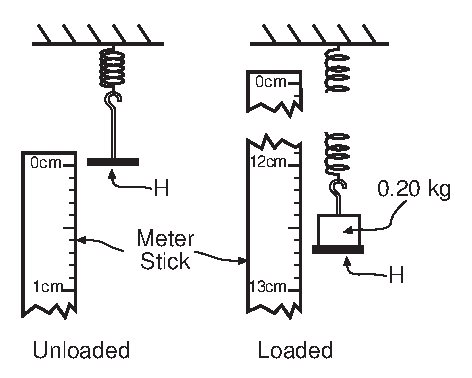
\includegraphics[keepaspectratio,scale=0.75]{Jan2001-Q10}
    \end{center}
    \begin{multicols}{2}
    \begin{choices}
        \wrongchoice{\SI{12.30}{\centi\meter}}
        \wrongchoice{\SI{12.50}{\centi\meter}}
      \correctchoice{\SI{12.70}{\centi\meter}}
        \wrongchoice{\SI{13.30}{\centi\meter}}
    \end{choices}
    \end{multicols}
\end{question}
}


%% Section June1999
%%--------------------

%% NOTE: June1999-Q21 utilizes a possible duplicate (I can change numbers),
%%  or tikz, they are just ovals after all?


%% Section June1997
%%--------------------
\element{nysed}{
\begin{question}{June1997-Q19}
    The graph below shows the relationship between the elongation of a spring and the force applied to the spring causing it to stretch.
    \begin{center}
    \begin{tikzpicture}
        \begin{axis}[
            axis y line=left,
            axis x line=bottom,
            axis line style={->},
            ylabel={elongation},
            y unit=\si{\meter},
            ytick={0,0.10,0.20,0.30,0.40,0.50,0.60},
            ymin=0,ymax=0.62,
            xlabel={Force},
            x unit=\si{\newton},
            xtick={0,10,20,30},
            xmin=0,xmax=30,
            grid=major,
            width=0.8\columnwidth,
            height=0.5\columnwidth,
            very thin,
        ]
        \addplot[line width=1pt,domain=0:30]{0.02*x};
        \end{axis}
    \end{tikzpicture}
    \end{center}
    What is the spring constant for this spring?
    \begin{multicols}{2}
    \begin{choices}
        \wrongchoice{\SI{0.020}{\newton\per\meter}}
        \wrongchoice{\SI{2.0}{\newton\per\meter}}
        \wrongchoice{\SI{25}{\newton\per\meter}}
      \correctchoice{\SI{50}{\newton\per\meter}}
    \end{choices}
    \end{multicols}
\end{question}
}


%% Section June1996
%%--------------------
\element{nysed}{
\begin{question}{June1996-Q20}
    A \SI{20}{\newton} weight is attached to a spring,
        causing it to stretch, as shown in the diagram below.
    \begin{center}
    \begin{tikzpicture}
        \begin{scope}[xshift=-2cm]
            %% Title
            \node[anchor=south,text centered] at (0.5,0.2cm) {Unstretched};
            %% Celiing
            \draw (-1,0) --  (2,0);
            \node[anchor=south,fill,pattern=north east lines,minimum width=3cm, minimum height=0.05cm] at (0.5,0) {};
            %% Spring
            \draw[thick,decoration={aspect=0.2,segment length=1.5mm,amplitude=4mm,coil},decorate] (0,0) -- (0,-1.5);
            \draw[dashed]  (0,-1.5) -- ++(0:1cm);
            %% Ruler
            \draw[<->] (1.5,0) -- (1.5,-1.5) node[pos=0.5,anchor=center,fill=white] {\SI{0.50}{\meter}};
        \end{scope}
        \begin{scope}[xshift=+2cm]
            %% Title
            \node[anchor=south,text centered] at (0.5,0.2cm) {Stretched};
            %% Celiing
            \draw (-1,0) --  (2,0);
            \node[anchor=south,fill,pattern=north east lines,minimum width=3cm, minimum height=0.05cm] at (0.5,0) {};
            %% Weight
            \node[anchor=north,draw,minimum size=1cm] (M) at (0,-3) {\SI{20}{\newton}};
            %% Spring
            \draw[thick,decoration={aspect=0.2,segment length=3mm,amplitude=4mm,coil},decorate] (0,0) -- (0,-3);
            \draw[dashed]  (0,-3) -- ++(0:1cm);
            %% Ruler
            \draw[<->] (1.5,0) -- (1.5,-3) node[pos=0.5,anchor=center,fill=white] {\SI{1.00}{\meter}};
        \end{scope}
    \end{tikzpicture}
    \end{center}
    What is the spring constant of this spring?
    \begin{multicols}{2}
    \begin{choices}
        \wrongchoice{\SI{0.050}{\newton\per\meter}}
        \wrongchoice{\SI{0.25}{\newton\per\meter}}
        \wrongchoice{\SI{20}{\newton\per\meter}}
      \correctchoice{\SI{40}{\newton\per\meter}}
    \end{choices}
    \end{multicols}
\end{question}
}


%% Section June1990
%%--------------------
\element{nysed}{
\begin{question}{June1990-Q22}
    The graph below represents the relationship between the force applied to a spring and the elongation of the spring.
    \begin{center}
    \begin{tikzpicture}
        \begin{axis}[
            axis y line=left,
            axis x line=bottom,
            axis line style={->},
            xlabel={elongation},
            x unit=\si{\meter},
            xtick={0,0.2,0.4,0.6,0.8},
            ylabel={force},
            y unit=\si{\newton},
            ytick={0,4,8,12,16},
            xmin=0,xmax=0.82,
            ymin=0,ymax=16.5,
            grid=major,
            width=0.8\columnwidth,
            height=0.5\columnwidth,
            very thin,
        ]
        \addplot[line width=1pt,domain=0:0.8]{20*x};
        \end{axis}
    \end{tikzpicture}
    \end{center}
    What is the spring constant?
    \begin{multicols}{2}
    \begin{choices}
      \correctchoice{\SI{20}{\newton\per\meter}}
        \wrongchoice{\SI{9.8}{\newton\per\meter}}
        \wrongchoice{\SI{0.80}{\newton\per\meter}}
        \wrongchoice{\SI{0.050}{\newton\per\meter}}
    \end{choices}
    \end{multicols}
\end{question}
}


\endinput



%
%% Vectors and Motion Questions used on the
%% NYSED Physics Regents Examination
%%--------------------------------------------------

%% this section contains 68 problems


%% Section June2015
%%--------------------
\element{nysed}{
\begin{question}{June2015-Q01}
    Which quantities are scalar?
    \begin{choices}
      \correctchoice{speed and work}
        \wrongchoice{velocity and force}
        \wrongchoice{distance and acceleration}
        \wrongchoice{momentum and power}
    \end{choices}
\end{question}
}

\element{nysed}{
\begin{question}{June2015-Q03}
    An airplane traveling north at \SI{220}{\meter\per\second} encounters a \SI{50.0}{\meter\per\second} crosswind from west to east,
        as represented in the diagram below.
    \begin{center}
        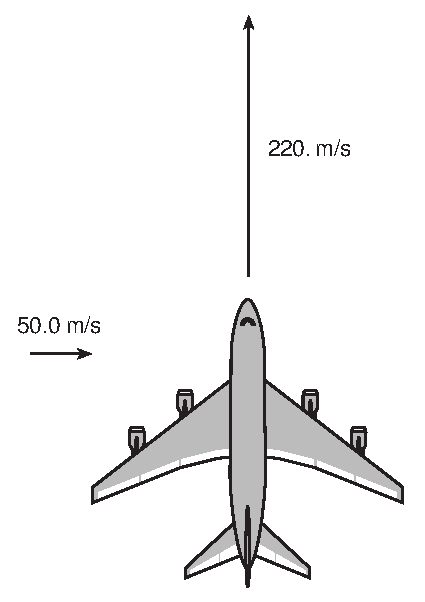
\includegraphics[keepaspectratio,scale=0.95]{June2015-Q03}
    \end{center}
    What is the resultant speed of the plane?
    \begin{multicols}{2}
    \begin{choices}
        \wrongchoice{\SI{170}{\meter\per\second}}
        \wrongchoice{\SI{214}{\meter\per\second}}
      \correctchoice{\SI{226}{\meter\per\second}}
        \wrongchoice{\SI{270}{\meter\per\second}}
    \end{choices}
    \end{multicols}
\end{question}
}

\element{nysed}{
\begin{question}{June2015-Q37}
    The vector diagram below represents the velocity of a car traveling \SI{24}{\meter\per\second} \ang{35} east of north.
    \begin{center}
    \begin{tikzpicture}
        \draw[dashed] (-1,0) -- (2,0) node[pos=0,anchor=east] {W} node[pos=1,anchor=west] {E};
        \draw[dashed] (0,-1) -- (0,2) node[pos=0,anchor=north] {S} node[pos=1,anchor=south] {N};
        \draw[thick,->] (0,0) -- ++(55:2.0cm);
        \draw[] (55:1.0cm) arc (55:90:1.0cm) node[pos=0.5,anchor=south,font=\small] {\ang{35}};
    \end{tikzpicture}
    \end{center}
    What is the magnitude of the component of the car's velocity that is directed eastward?
    \begin{multicols}{2}
    \begin{choices}
      \correctchoice{\SI{14}{\meter\per\second}}
        \wrongchoice{\SI{20}{\meter\per\second}}
        \wrongchoice{\SI{29}{\meter\per\second}}
        \wrongchoice{\SI{42}{\meter\per\second}}
    \end{choices}
    \end{multicols}
\end{question}
}


%% Section June2014
%%--------------------
\element{nysed}{
\begin{question}{June2014-Q01}
    Which quantity is scalar?
    \begin{multicols}{2}
    \begin{choices}
      \correctchoice{mass}
        \wrongchoice{force}
        \wrongchoice{momentum}
        \wrongchoice{acceleration}
    \end{choices}
    \end{multicols}
\end{question}
}

\element{nysed}{
\begin{question}{June2014-Q03}
    The components of a \SI{15}{\meter\per\second} velocity at an angle of \ang{60} above the horizontal are:
    \begin{choices}
      \correctchoice{\SI{13}{\meter\per\second} vertical and \SI{7.5}{\meter\per\second} horizontal}
        \wrongchoice{\SI{7.5}{\meter\per\second} vertical and \SI{13}{\meter\per\second} horizontal}
        \wrongchoice{\SI{6.0}{\meter\per\second} vertical and \SI{9.0}{\meter\per\second} horizontal}
        \wrongchoice{\SI{9.0}{\meter\per\second} vertical and \SI{6.0}{\meter\per\second} horizontal}
    \end{choices}
\end{question}
}


%% Section June2013
%%--------------------
\element{nysed}{
\begin{question}{June2013-Q02}
    Two \SI{20}{\newton} forces act concurrently on an object.
    What angle between these forces will produce a resultant force with the greatest magnitude?
    \begin{multicols}{4}
    \begin{choices}
      \correctchoice{\ang{0}}
        \wrongchoice{\ang{45}}
        \wrongchoice{\ang{90}}
        \wrongchoice{\ang{180}}
    \end{choices}
    \end{multicols}
\end{question}
}


%% Section June2012
%%--------------------
\element{nysed}{
\begin{question}{June2012-Q03}
    A baseball is thrown at an angle of \SI{40.0} above the horizontal.
    The horizontal component of the baseball's initial velocity is \SI{12.0}{\meter\per\second}.
    What is the magnitude of the ball's initial velocity?
    \begin{multicols}{2}
    \begin{choices}
        \wrongchoice{\SI{7.71}{\meter\per\second}}
        \wrongchoice{\SI{9.20}{\meter\per\second}}
      \correctchoice{\SI{15.7}{\meter\per\second}}
        \wrongchoice{\SI{18.7}{\meter\per\second}}
    \end{choices}
    \end{multicols}
\end{question}
}


%% Section June2011
%%--------------------
\element{nysed}{
\begin{question}{June2011-Q01}
    Scalar is to vector as:
    \begin{choices}
      \correctchoice{speed is to velocity}
        \wrongchoice{displacement is to distance}
        \wrongchoice{displacement is to velocity}
        \wrongchoice{speed is to distance}
    \end{choices}
\end{question}
}


%% Section June2010
%%--------------------
\element{nysed}{
\begin{question}{June2010-Q02}
    A motorboat, which has a speed of \SI{5.0}{\meter\per\second} in still water,
        is headed east as it crosses a river flowing south at \SI{3.3}{\meter\per\second}.
    What is the magnitude of the boat's resultant velocity with respect to the starting point?
    \begin{multicols}{2}
    \begin{choices}
        \wrongchoice{\SI{3.3}{\meter\per\second}}
        \wrongchoice{\SI{6.0}{\meter\per\second}}
      \correctchoice{\SI{5.0}{\meter\per\second}}
        \wrongchoice{\SI{8.3}{\meter\per\second}}
    \end{choices}
    \end{multicols}
\end{question}
}


%% Section June2009
%%--------------------
\element{nysed}{
\begin{question}{June2009-Q02}
    The vector diagram below represents the horizontal component, $F_H$,
        and the vertical component, $F_V$, of a \SI{24}{\newton} force acting at \ang{35} above the horizontal.
    \begin{center}
    \begin{tikzpicture}[scale=1.5]
        \draw[thick,->] (0,0) -- (0,1.38) node[pos=0.5,anchor=east] {$F_V$};
        \draw[thick,->] (0,0) -- (1.97,0) node[pos=0.5,anchor=north] {$F_H$} node[pos=0.25,anchor=south west] {\ang{35}};
        \draw[thick,dashed] (0,1.38) -- (1.97,1.38);
        \draw[thick,dashed] (1.97,0) -- (1.97,1.38);
        \draw[thick,->] (0,0) -- (1.97,1.38) node[pos=0.5,anchor=south,rotate=35] {\SI{24}{\newton}};
    \end{tikzpicture}
    \end{center}
    What are the magnitudes of the horizontal and vertical components?
    \begin{choices}
        \wrongchoice{$F_H=\SI{3.5}{\newton}$ and $F_V=\SI{4.9}{\newton}$}
        \wrongchoice{$F_H=\SI{4.9}{\newton}$ and $F_V=\SI{3.5}{\newton}$}
        \wrongchoice{$F_H=\SI{14}{\newton}$ and $F_V=\SI{20.}{\newton}$}
      \correctchoice{$F_H=\SI{20.}{\newton}$ and $F_V=\SI{14}{\newton}$}
    \end{choices}
\end{question}
}


%% Section June2008
%%--------------------
\element{nysed}{
\begin{question}{June2008-Q01}
    The speedometer in a car does \emph{not} measure the car's velocity because velocity is a:
    \begin{choices}
      \correctchoice{vector quantity and has a direction associated with it}
        \wrongchoice{vector quantity and does not have a direction associated with it}
        \wrongchoice{scalar quantity and has a direction associated with it}
        \wrongchoice{scalar quantity and does not has a direction associated with it}
    \end{choices}
\end{question}
}

\element{nysed}{
\begin{question}{June2008-Q11}
    An airplane flies with a velocity of \SI{750}{\kilo\meter\per\hour},
        \ang{30} south of east.
    What is the magnitude of the eastward component of the plane's velocity?
    \begin{multicols}{2}
    \begin{choices}
        \wrongchoice{\SI{866}{\kilo\meter\per\hour}}
      \correctchoice{\SI{650}{\kilo\meter\per\hour}}
        \wrongchoice{\SI{433}{\kilo\meter\per\hour}}
        \wrongchoice{\SI{375}{\kilo\meter\per\hour}}
    \end{choices}
    \end{multicols}
\end{question}
}

\element{nysed}{
\begin{question}{June2008-Q41}
    The diagram below represents two concurrent forces.
    \begin{center}
    \begin{tikzpicture}[scale=0.60]
        \draw[very thick,->] (0,0) -- (0,3);
        \draw[very thick,->] (0,0) -- (-4,0);
    \end{tikzpicture}
    \end{center}
    Which vector represents the force that will produce equilibrium with these two forces?
    \begin{multicols}{2}
    \begin{choices}
        \AMCboxDimensions{down=-0.9cm}
        \wrongchoice{
            \begin{tikzpicture}[scale=0.60]
                \draw[dashed,white!90!black] (0.5,0) rectangle (-4.5,3);
                \draw[very thick,->] (0,0) -- (-4,3);
            \end{tikzpicture}
        }
        \wrongchoice{
            \begin{tikzpicture}[scale=0.60]
                \draw[dashed,white!90!black] (-0.5,0) rectangle (4.5,3);
                \draw[very thick,->] (0,0) -- (4,3);
            \end{tikzpicture}
        }
        %% ANS is 3
        \correctchoice{
            \begin{tikzpicture}[scale=0.60]
                \draw[dashed,white!90!black] (-0.5,0) rectangle (4.5,-3);
                \draw[very thick,->] (0,0) -- (4,-3);
            \end{tikzpicture}
        }
        \wrongchoice{
            \begin{tikzpicture}[scale=0.60]
                \draw[dashed,white!90!black] (0,-1.5) rectangle (-5,1.5);
                \draw[very thick,->] (0,0) -- (-5,0);
            \end{tikzpicture}
        }
    \end{choices}
    \end{multicols}
\end{question}
}


%% Section Jan2008
%%--------------------
\element{nysed}{
\begin{question}{Jan2008-Q01}
    Which is a vector quantity?
    \begin{multicols}{2}
    \begin{choices}
        \wrongchoice{speed}
        \wrongchoice{mass}
        \wrongchoice{work}
      \correctchoice{displacement}
    \end{choices}
    \end{multicols}
\end{question}
}

\element{nysed}{
\begin{question}{Jan2008-Q04}
    A soccer player kicks a ball with an initial velocity
        of \SI{10}{\meter\per\second} at an angle of
        \ang{30} above the horizontal.
    The magnitude of the horizontal component of the ball's
        initial velocity is:
    \begin{multicols}{2}
    \begin{choices}
      \correctchoice{\SI{8.7}{\meter\per\second}}
        \wrongchoice{\SI{5.0}{\meter\per\second}}
        \wrongchoice{\SI{9.8}{\meter\per\second}}
        \wrongchoice{\SI{10}{\meter\per\second}}
    \end{choices}
    \end{multicols}
\end{question}
}

\element{nysed}{
\begin{question}{Jan2008-Q38}
    Two forces act concurrently on an object.
    Their resultant force has the largest magnitude when
        the angle between the forces is:
    \begin{multicols}{2}
    \begin{choices}
      \correctchoice{\ang{0}}
        \wrongchoice{\ang{90}}
        \wrongchoice{\ang{30}}
        \wrongchoice{\ang{180}}
    \end{choices}
    \end{multicols}
\end{question}
}


%% Section June2007
%%--------------------
\element{nysed}{
\begin{question}{June2007-Q05}
    As the angle between two concurrent forces decreases,
        the magnitude of the force required to produce equilibrium
    \begin{multicols}{2}
    \begin{choices}
        \wrongchoice{decreases}
      \correctchoice{increases}
        \wrongchoice{remains the same}
    \end{choices}
    \end{multicols}
\end{question}
}

\element{nysed}{
\begin{question}{June2007-Q06}
    A child walks \SI{5.0}{\meter} north, then \SI{4.0}{\meter} east,
        and finally \SI{2.0}{\meter} south.
    What is the magnitude of the resultant displacement of the child after
        the entire walk?
    \begin{multicols}{2}
    \begin{choices}
      \correctchoice{\SI{5.0}{\meter}}
        \wrongchoice{\SI{1.0}{\meter}}
        \wrongchoice{\SI{3.0}{\meter}}
        \wrongchoice{\SI{11.0}{\meter}}
    \end{choices}
    \end{multicols}
\end{question}
}

\element{nysed}{
\begin{question}{June2007-Q38}
    A stream is \SI{30}{\meter} wide and it current flows southward at
        \SI{1.5}{\meter\per\second}.
    A toy boat is launched with a velocity of
        \SI{2.0}{\meter\per\second} eastward from the west bank of the stream.
    What is the magnitude of the boat's resultant velocity as it crossed the stream?
    \begin{multicols}{2}
    \begin{choices}
        \wrongchoice{\SI{0.5}{\meter\per\second}}
      \correctchoice{\SI{2.5}{\meter\per\second}}
        \wrongchoice{\SI{3.0}{\meter\per\second}}
        \wrongchoice{\SI{3.5}{\meter\per\second}}
    \end{choices}
    \end{multicols}
\end{question}
}

\element{nysed}{
\begin{question}{June2007-Q39}
    A stream is \SI{30}{\meter} wide and it current flows southward at
        \SI{1.5}{\meter\per\second}.
    A toy boat is launched with a velocity of \SI{2.0}{\meter\per\second}
        eastward from the west bank of the stream.
    How much time is required for the boat to reach the opposite
        bank of the stream?
    \begin{multicols}{2}
    \begin{choices}
        \wrongchoice{\SI{8.6}{\second}}
        \wrongchoice{\SI{12}{\second}}
      \correctchoice{\SI{15}{\second}}
        \wrongchoice{\SI{60}{\second}}
    \end{choices}
    \end{multicols}
\end{question}
}

%% Section Jan2007
%%--------------------
\element{nysed}{
\begin{question}{Jan2007-Q02}
    A \SI{6.0}{\newton} force and an \SI{8.0}{\newton} force act
        concurrently on a point.
    As the angle between these forces increases from \ang{0} to \ang{90},
        the magnitude of their resultant:
    \begin{choices}
      \correctchoice{decreases}
        \wrongchoice{increases}
        \wrongchoice{remains the same}
    \end{choices}
\end{question}
}


%% Section June2006
%%--------------------
\element{nysed}{
\begin{question}{June2006-Q03}
    The diagram below represents a force vector, $A$, and a
        resultant vector, $R$.
    \begin{center}
        \begin{tikzpicture}
            \draw[thick,->] (0,0) -- (0,2cm);
            \node[thick,anchor=west] at (0,1cm) {$A$};
        \end{tikzpicture}
        \begin{tikzpicture}
            \draw[thick,->] (0,0) -- (55:3.28cm);
            \node[thick,anchor=north,xshift=2pt] at (55:1.64cm) {$R$};
        \end{tikzpicture}
    \end{center}
    Which force vector $B$ below could be added to force vector
        $A$ to produce resultant vector $R$?
    \begin{multicols}{2}
    \begin{choices}
        \AMCboxDimensions{down=-1.0em}
        \correctchoice{
            \begin{tikzpicture}
                \draw[thick,->] (0,0) -- (20:2cm);
                \node[thick,anchor=north] at (20:1cm) {$B$};
            \end{tikzpicture}
        }
        \wrongchoice{
            \begin{tikzpicture}
                \draw[thick,->] (0,0) -- (160:2cm);
                \node[thick,anchor=north] at (160:1cm) {$B$};
            \end{tikzpicture}
        }
        \wrongchoice{
            \begin{tikzpicture}
                \draw[thick,->] (0,0) -- (-20:2cm);
                \node[thick,anchor=north] at (-20:1cm) {$B$};
            \end{tikzpicture}
        }
        \wrongchoice{
            \begin{tikzpicture}
                \draw[thick,->] (0,0) -- (200:2cm);
                \node[thick,anchor=north] at (200:1cm) {$B$};
            \end{tikzpicture}
        }
    \end{choices}
    \end{multicols}
\end{question}
}

\element{nysed}{
\begin{question}{June2006-Q04}
    A golf ball is propelled with an initial velocity of
        \SI{60}{\meter\per\second} at \ang{37} above the horizontal.
    The horizontal component of the golf ball's initial velocity is:
    \begin{multicols}{2}
    \begin{choices}
      \correctchoice{\SI{48}{\meter\per\second}}
        \wrongchoice{\SI{40}{\meter\per\second}}
        \wrongchoice{\SI{30}{\meter\per\second}}
        \wrongchoice{\SI{36}{\meter\per\second}}
    \end{choices}
    \end{multicols}
\end{question}
}

\element{nysed}{
\begin{question}{June2006-Q06}
    A \SI{3}{\newton} force and a \SI{4}{\newton} force are acting concurrently on a point.
    Which force could not produce equilibrium with these two forces?
    \begin{multicols}{2}
    \begin{choices}
        \wrongchoice{\SI{1}{\newton}}
        \wrongchoice{\SI{7}{\newton}}
      \correctchoice{\SI{9}{\newton}}
        \wrongchoice{\SI{4}{\newton}}
    \end{choices}
    \end{multicols}
\end{question}
}


%% Section Jan2006
%%--------------------
\element{nysed}{
\begin{question}{Jan2006-Q04}
    A projectile is fired with an initial velocity of
        \SI{120}{\meter\per\second}
        at an angle, $\theta$, above the horizontal.
    If the projectile's initial horizontal speed is
        \SI{55}{\meter\per\second}, then angle $\theta$
        measures approximately:
    \begin{multicols}{4}
    \begin{choices}
      \correctchoice{\ang{63}}
        \wrongchoice{\ang{75}}
        \wrongchoice{\ang{27}}
        \wrongchoice{\ang{13}}
    \end{choices}
    \end{multicols}
\end{question}
}

\element{nysed}{
\begin{question}{Jan2006-Q03}
    Which is a scalar quantity?
    \begin{multicols}{2}
    \begin{choices}
      \correctchoice{speed}
        \wrongchoice{acceleration}
        \wrongchoice{displacement}
        \wrongchoice{momentum}
    \end{choices}
    \end{multicols}
\end{question}
}

\element{nysed}{
\begin{question}{Jan2006-Q12}
    A student on her way to school walks four blocks east,
        three block north, and another four blocks east,
        as shown in the diagram.
    \begin{center}
        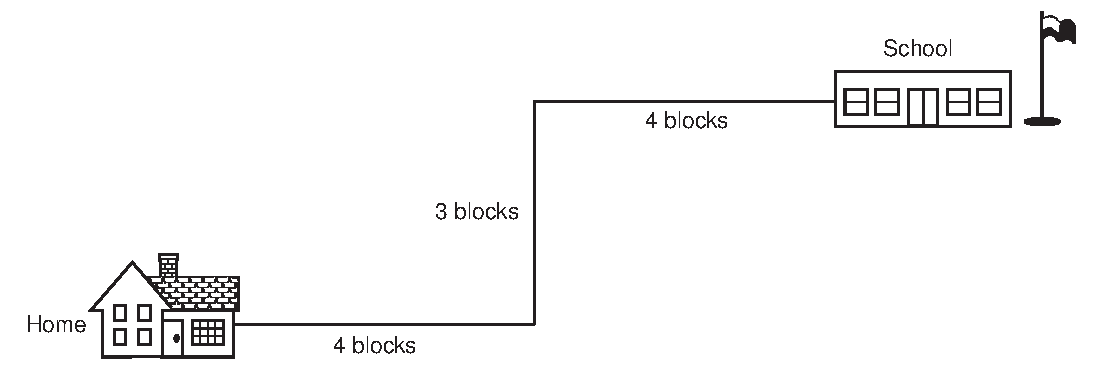
\includegraphics[keepaspectratio,width=\linewidth]{Jan2006-Q12}
    \end{center}
    Compared to the distance she walks,
        the magnitude of her displacement home to school is:
    \begin{multicols}{3}
    \begin{choices}
      \correctchoice{less}
        \wrongchoice{more}
        \wrongchoice{the same}
    \end{choices}
    \end{multicols}
\end{question}
}

\element{nysed}{
\begin{question}{Jan2006-Q46}
    Two \SI{30}{\newton} forces act concurrently on an object.
    In which diagram would the forces produce a
        resultant with a magnitude of \SI{30}{\newton}?
    \begin{multicols}{2}
    \begin{choices}
        \AMCboxDimensions{down=-1.0em}
        \correctchoice{
            \begin{tikzpicture}[scale=0.9]
                \draw[dashed,white!90!black] (-1.5cm,-2em) rectangle (1.5cm,1.5cm);
                \draw[fill] (0,0) circle [radius=0.5em];
                \node[anchor=south west] at (15:0.1cm) {\ang{120}};
                \draw[thick,->] (0,0) -- (0:1.5cm);
                \node[anchor=north] at (0:0.8cm) {\SI{30}{\newton}};
                \draw[thick,->] (0,0) -- (120:1.5cm);
                \node[anchor=north east] at (120:0.8cm) {\SI{30}{\newton}};
            \end{tikzpicture}
        }
        \wrongchoice{
            \begin{tikzpicture}[scale=0.9]
                \draw[dashed,white!90!black] (-1.5cm,-2em) rectangle (1.5cm,1.5cm);
                \draw[fill] (0,0) circle [radius=0.5em];
                \node[anchor=south west] at (15:0.2cm) {\ang{60}};
                \draw[thick,->] (0,0) -- (0:1.5cm);
                \node[anchor=north] at (0:0.8cm) {\SI{30}{\newton}};
                \draw[thick,->] (0,0) -- (60:1.5cm);
                \node[anchor=south east] at (60:0.8cm) {\SI{30}{\newton}};
            \end{tikzpicture}
        }
        \wrongchoice{
            \begin{tikzpicture}[scale=0.9]
                \draw[dashed,white!90!black] (-1.5cm,-2em) rectangle (1.5cm,1.5cm);
                \draw[fill] (0,0) circle [radius=0.5em];
                \node[anchor=south west] at (4:0.75cm) {\ang{30}};
                \draw[thick,->] (0,0) -- (0:1.5cm);
                \node[anchor=north] at (0:0.8cm) {\SI{30}{\newton}};
                \draw[thick,->] (0,0) -- (30:1.5cm);
                \node[anchor=south east] at (30:0.8cm) {\SI{30}{\newton}};
            \end{tikzpicture}
        }
        \wrongchoice{
            \begin{tikzpicture}[scale=0.9]
                \draw[dashed,white!90!black] (-1.5cm,-2em) rectangle (1.5cm,1.5cm);
                \draw[fill] (0,0) circle [radius=0.5em];
                \node[anchor=south] at (90:0.2cm) {\ang{180}};
                \draw[thick,->] (0,0) -- (0:1.5cm);
                \node[anchor=north] at (0:0.8cm) {\SI{30}{\newton}};
                \draw[thick,->] (0,0) -- (180:1.5cm);
                \node[anchor=north] at (180:0.8cm) {\SI{30}{\newton}};
            \end{tikzpicture}
        }
    \end{choices}
    \end{multicols}
\end{question}
}


%% Section June2005
%%--------------------
\element{nysed}{
\begin{question}{June2005-Q03}
    A \SI{5.0}{\newton} force and a \SI{7.0}{\newton} force act concurrently on a point.
    As the angle between the forces is increased from \ang{0} to \ang{180},
        the magnitude of the resultant of the two forces changes from:
    \begin{multicols}{2}
    \begin{choices}
      \correctchoice{\SI{12.0}{\newton} to \SI{2.0}{\newton}}
        \wrongchoice{\SI{0.0}{\newton} to \SI{12.0}{\newton}}
        \wrongchoice{\SI{2.0}{\newton} to \SI{12.0}{\newton}}
        \wrongchoice{\SI{12.0}{\newton} to \SI{0.0}{\newton}}
    \end{choices}
    \end{multicols}
\end{question}
}

\element{nysed}{
\begin{question}{June2005-Q04}
    A \SI{5.0}{\newton} force could have perpendicular components of:
    \begin{multicols}{2}
    \begin{choices}
      \correctchoice{\SI{3.0}{\newton} and \SI{4.0}{\newton}}
        \wrongchoice{\SI{1.0}{\newton} and \SI{4.0}{\newton}}
        \wrongchoice{\SI{2.0}{\newton} and \SI{3.0}{\newton}}
        \wrongchoice{\SI{5.0}{\newton} and \SI{5.0}{\newton}}
    \end{choices}
    \end{multicols}
\end{question}
}


%% Section Jan2005
%%--------------------
\element{nysed}{
\begin{question}{Jan2005-Q03}
    A golf ball is hit with an initial velocity of \SI{15}{\meter\per\second} at an angle of \ang{35} above the horizontal.
    What is the vertical component of the gold ball's initial velocity?
    \begin{multicols}{2}
    \begin{choices}
      \correctchoice{\SI{8.6}{\meter\per\second}}
        \wrongchoice{\SI{9.8}{\meter\per\second}}
        \wrongchoice{\SI{12}{\meter\per\second}}
        \wrongchoice{\SI{15}{\meter\per\second}}
    \end{choices}
    \end{multicols}
\end{question}
}

\element{nysed}{
\begin{question}{Jan2005-Q37}
    The vector below represents two forces, $F_1$ and $F_2$, simultaneously acting on an object.
    \begin{center}
    \begin{tikzpicture}[scale=0.75]
        \draw[thick,->] (0,0) -- (230:2cm)
            node[pos=0.5,anchor=south east] {$F_1$};
        \draw[thick,->] (0,0) -- (320:3cm)
            node[pos=0.5,anchor=south west] {$F_2$};
    \end{tikzpicture}
    \end{center}
    Which vector best represents the resultant of the two forces?
    \begin{multicols}{2}
    \begin{choices}
        \AMCboxDimensions{down=-1.5em}
        \correctchoice{
            \begin{tikzpicture}[scale=0.75]
                \draw[dashed,white!90!black] (-1.00,-3.5) rectangle (2.50,0);
                \draw[thick,->] (0,0) -- (286:3.6cm)
                    node[pos=0.5,anchor=east] {$R$};
            \end{tikzpicture}
        }
        \wrongchoice{
            \begin{tikzpicture}[scale=0.75]
                \draw[dashed,white!90!black] (+1.00,+3.5) rectangle (-2.50,-0);
                \draw[thick,->] (0,0) -- (106:3.6cm)
                    node[pos=0.5,anchor=east] {$R$};
            \end{tikzpicture}
        }
        \wrongchoice{
            \begin{tikzpicture}[scale=0.75]
                \draw[dashed,white!90!black] (+0.25,+2) rectangle (-3.75,-1.5);
                \draw[thick,->] (0,0) -- (176:3.6cm)
                    node[pos=0.5,anchor=south west] {$R$};
            \end{tikzpicture}
        }
        \wrongchoice{
            \begin{tikzpicture}[scale=0.75]
                \draw[dashed,white!90!black] (-0.25,-2) rectangle (3.75,1.5);
                \draw[thick,->] (0,0) -- (356:3.6cm)
                    node[pos=0.5,anchor=south west] {$R$};
            \end{tikzpicture}
        }
    \end{choices}
    \end{multicols}
\end{question}
}


%% Section June2004
%%--------------------
\element{nysed}{
\begin{question}{June2004-Q01}
    Velocity is to speed as displacement is to:
    \begin{multicols}{2}
    \begin{choices}
      \correctchoice{distance}
        \wrongchoice{acceleration}
        \wrongchoice{time}
        \wrongchoice{momentum}
    \end{choices}
    \end{multicols}
\end{question}
}

\element{nysed}{
\begin{question}{June2004-Q02}
    The diagram below shows a resultant vector, $R$.
    \begin{center}
    \begin{tikzpicture}[scale=0.9]
        \draw[thick,->] (0,0) -- (135:2cm)
            node[pos=0.5,anchor=south west] {$R$};
    \end{tikzpicture}
    \end{center}
    Which diagram best represents a pair of component vectors, $A$ and $B$,
        that would combine to form resultant vector $R$?
    \begin{multicols}{2}
    \begin{choices}
        \AMCboxDimensions{down=-0.5cm}
        \correctchoice{
            \begin{tikzpicture}[scale=0.9]
                \draw[dashed,white!90!black] (-1.5cm,-1em) rectangle (1.5cm,1.5cm);
                \draw[thick,->] (0,0) -- (90:1.5cm)
                    node[pos=0.5,anchor=east] {$A$};
                \draw[thick,->] (0,0) -- (180:1.5cm)
                    node[pos=0.5,anchor=north west] {$B$};
            \end{tikzpicture}
        }
        \wrongchoice{
            \begin{tikzpicture}[scale=0.9]
                \draw[dashed,white!90!black] (-1.5cm,-1em) rectangle (1.5cm,1.5cm);
                \draw[thick,->] (0,0) -- (90:1.5cm)
                    node[pos=0.5,anchor=east] {$A$};
                \draw[thick,->] (0,0) -- (45:1.5cm)
                    node[pos=0.5,anchor=north west] {$B$};
            \end{tikzpicture}
        }
        \wrongchoice{
            \begin{tikzpicture}[scale=0.9]
                \draw[dashed,white!90!black] (-1.5cm,-1em) rectangle (1.5cm,1.5cm);
                \draw[thick,->] (0,0) -- (90:1.5cm)
                    node[pos=0.5,anchor=west] {$A$};
                \draw[thick,->] (0,0) -- (0:1.5cm)
                    node[pos=0.5,anchor=north] {$B$};
            \end{tikzpicture}
        }
        \wrongchoice{
            \begin{tikzpicture}[scale=0.9]
                \draw[dashed,white!90!black] (-1.5cm,-1em-0.50cm) rectangle (1.5cm,1.00cm);
                \draw[thick,->] (-0.1cm,0) -- (180:1.5cm)
                    node[pos=0.5,anchor=north] {$A$};
                \draw[thick,->] (0.1cm,0) -- (0:1.5cm)
                    node[pos=0.5,anchor=north] {$B$};
            \end{tikzpicture}
        }
    \end{choices}
    \end{multicols}
\end{question}
}


%% Section Jan2004
%%--------------------
\element{nysed}{
\begin{question}{Jan2004-Q01}
    A girl leaves a history classroom and walks \SI{10}{\meter} north to a drinking fountain.
    Then she turns and walks \SI{30}{\meter} south to an art classroom.
    What is the girl's total displacement from the history classroom to the art classroom?
    \begin{multicols}{2}
    \begin{choices}
      \correctchoice{\SI{20.}{\meter} south}
        \wrongchoice{\SI{20.}{\meter} north}
        \wrongchoice{\SI{40.}{\meter} south}
        \wrongchoice{\SI{40.}{\meter} north}
    \end{choices}
    \end{multicols}
\end{question}
}

\element{nysed}{
\begin{question}{Jan2004-Q02}
    One car travels \SI{40}{\meter} due east in \SI{5.0}{\second},
        and a second car travels \SI{64}{\meter} due west in \SI{8.0}{\second}.
    During their periods of travel, the cars definitely had the same
    \begin{choices}
      \correctchoice{average speed}
        \wrongchoice{average velocity}
        \wrongchoice{total displacement}
        \wrongchoice{change in momentum}
    \end{choices}
\end{question}
}

\element{nysed}{
\begin{question}{Jan2004-Q39}
    The diagram below represents a \SI{5.0}{\newton} force and a \SI{12}{\newton} force acting on point $P$.
    \begin{center}
    \begin{tikzpicture}
        \node[anchor=north east] at (0:0) {$P$};
        \draw[fill] (0,0) circle [radius=2pt];
        \draw[thick,->] (0,0) -- (90:2cm);
        \node[anchor=south,rotate=90] at (90:1cm) {\SI{5}{\newton}};
        \draw[thick,->] (0,0) -- (0:4.8cm);
        \node[anchor=north] at (0:2.4cm) {\SI{12}{\newton}};
    \end{tikzpicture}
    \end{center}
    The resultant of the two forces has magnitude of:
    \begin{multicols}{2}
    \begin{choices}
      \correctchoice{\SI{13}{\newton}}
        \wrongchoice{\SI{12}{\newton}}
        \wrongchoice{\SI{5.0}{\newton}}
        \wrongchoice{\SI{7.0}{\newton}}
    \end{choices}
    \end{multicols}
\end{question}
}


%% Section June2003
%%--------------------
\element{nysed}{
\begin{question}{June2003-Q02}
    A vector makes an angle $\theta$ with the horizontal.
    The horizontal and vertical components of the vector will be equal in magnitude if angle $\theta$ is:
    \begin{multicols}{4}
    \begin{choices}
      \correctchoice{\ang{45}}
        \wrongchoice{\ang{30}}
        \wrongchoice{\ang{60}}
        \wrongchoice{\ang{90}}
    \end{choices}
    \end{multicols}
\end{question}
}

\element{nysed}{
\begin{question}{June2003-Q36}
    Force $A$ and $B$ have a resultant $R$. 
    Force $A$ and resultant $R$ are represented in the diagram below.
    \begin{center}
    \begin{tikzpicture}
        \draw[thick,->] (0,0) -- (14.47:2cm);
        \node[anchor=south east] at (14.47:1cm) {$R$};
        \draw[thick,->] (0,0) -- (-30:2cm);
        \node[anchor=north east] at (-30:1cm) {$A$};
    \end{tikzpicture}
    \end{center}
    Which vector best represents force $B$?
    \begin{multicols}{2}
    \begin{choices}
        \AMCboxDimensions{down=-0.5cm}
        \correctchoice{
            \begin{tikzpicture}
                \draw[draw=white] (-0.75,0) rectangle (0.75,1);
                \draw[thick,->] (0,0) -- (90:1cm)
                    node[pos=0.5,anchor=east] {$B$};
            \end{tikzpicture}
        }
        \wrongchoice{
            \begin{tikzpicture}
                \draw[draw=white] (-0.25,-0.5) rectangle (-1.25,0.5);
                \draw[thick,->] (0,0) -- (180:1cm)
                    node[pos=0.5,anchor=south] {$B$};
            \end{tikzpicture}
        }
        \wrongchoice{
            \begin{tikzpicture}
                \draw[draw=white] (-0.75,0) rectangle (0.75,-1);
                \draw[thick,->] (0,0) -- (270:1cm)
                    node[pos=0.5,anchor=east] {$B$};
            \end{tikzpicture}
        }
        \wrongchoice{
            \begin{tikzpicture}
                \draw[draw=white] (-0.25,-0.5) rectangle (1.25,0.5);
                \draw[thick,->] (0,0) -- (0:1cm)
                    node[pos=0.5,anchor=south] {$B$};
            \end{tikzpicture}
        }
    \end{choices}
    \end{multicols}
\end{question}
}


%% Section Jan2003
%%--------------------
\element{nysed}{
\begin{question}{Jan2003-Q02}
    A car travels \SI{90}{\meter} due north in \SI{15}{\second}.
    Then the car turns around and travels \SI{40}{\meter} due south in \SI{5.0}{\second}.
    What is the magnitude of the average velocity of the car during this \SI{20}{\second} interval?
    \begin{multicols}{2}
    \begin{choices}
      \correctchoice{\SI{2.5}{\meter\per\second}}
        \wrongchoice{\SI{5.0}{\meter\per\second}}
        \wrongchoice{\SI{6.5}{\meter\per\second}}
        \wrongchoice{\SI{7.0}{\meter\per\second}}
    \end{choices}
    \end{multicols}
\end{question}
}

\element{nysed}{
\begin{question}{Jan2003-Q36}
    Which pair of forces acting concurrently on an object will produce the resultant of greatest magnitude?
    \begin{multicols}{2}
    \begin{choices}
        \AMCboxDimensions{down=-0.5em}
        \correctchoice{
            \begin{tikzpicture}
                \draw[thick,->] (0,0) -- (90:1.25cm);
                \node[anchor=west] at (90:0.625cm) {\SI{4.0}{\newton}};
            \end{tikzpicture}
            \begin{tikzpicture}
                \draw[thick,->] (0,0) -- (135:1.875cm);
                \node[anchor=north east] at (135:0.9375cm) {\SI{6.0}{\newton}};
            \end{tikzpicture}
        }
        \wrongchoice{
            \begin{tikzpicture}
                \draw[thick,->] (0,0) -- (180:1.25cm);
                \node[anchor=south] at (180:0.625cm) {\SI{4.0}{\newton}};
            \end{tikzpicture}
            \begin{tikzpicture}
                \draw[thick,->] (0,0) -- (-45:1.875cm);
                \node[anchor=north east] at (-45:0.9375cm) {\SI{6.0}{\newton}};
            \end{tikzpicture}
        }
        \wrongchoice{
            \begin{tikzpicture}
                \draw[thick,->] (0,0) -- (0:1.25cm);
                \node[anchor=south] at (0:0.625cm) {\SI{4.0}{\newton}};
            \end{tikzpicture}
            \begin{tikzpicture}
                \draw[thick,->] (0,0) -- (180:1.875cm);
                \node[anchor=south] at (180:0.9375cm) {\SI{6.0}{\newton}};
            \end{tikzpicture}
        }
        \wrongchoice{
            \begin{tikzpicture}
                \draw[thick,->] (0,0) -- (270:1.25cm);
                \node[anchor=west] at (270:0.625cm) {\SI{4.0}{\newton}};
            \end{tikzpicture}
            \begin{tikzpicture}
                \draw[thick,->] (0,0) -- (0:1.875cm);
                \node[anchor=south] at (0:0.9375cm) {\SI{6.0}{\newton}};
            \end{tikzpicture}
        }
    \end{choices}
    \end{multicols}
\end{question}
}


%% Section Aug2002
%%--------------------
\element{nysed}{
\begin{question}{Aug2002-Q07}
    Which term represents a scalar quantity?
    \begin{multicols}{2}
    \begin{choices}
      \correctchoice{distance}
        \wrongchoice{displacement}
        \wrongchoice{force}
        \wrongchoice{weight}
    \end{choices}
    \end{multicols}
\end{question}
}

\element{nysed}{
\begin{question}{Aug2002-Q40}
    Which vector diagram represents the greatest magnitude of displacement for an object?
    \begin{multicols}{2}
    \begin{choices}
        \AMCboxDimensions{down=-1.3cm}
        \wrongchoice{
            \begin{tikzpicture}[scale=2]
                \draw[dashed,white!90!black] (-1.3,-0.4) rectangle (0.3,1.3);
                \draw[very thick,->] (0,0) -- (0,1) node[pos=0.5,anchor=south,rotate=-90] {\SI{1}{\meter}};
            \end{tikzpicture}
        }
        \correctchoice{
            \begin{tikzpicture}[scale=2]
                \draw[dashed,white!90!black] (-1.3,-0.4) rectangle (0.3,1.3);
                \draw[very thick,->] (0,0) -- (0,1) node[pos=0.5,anchor=south,rotate=-90] {\SI{1}{\meter}};
                \draw[very thick,->] (0,1) -- (-1,1) node[pos=0.5,anchor=south] {\SI{1}{\meter}};
            \end{tikzpicture}
        }
        \wrongchoice{
            \begin{tikzpicture}[scale=2]
                \draw[dashed,white!90!black] (-1.3,-0.4) rectangle (0.3,1.3);
                \draw[very thick,->] (0,0) -- (0,1) node[pos=0.5,anchor=south,rotate=-90] {\SI{1}{\meter}};
                \draw[very thick,->] (0,1) -- (-1,1) node[pos=0.5,anchor=south] {\SI{1}{\meter}};
                \draw[very thick,->] (-1,1) -- (-1,0) node[pos=0.5,rotate=90,anchor=south] {\SI{1}{\meter}};
            \end{tikzpicture}
        }
        \wrongchoice{
            \begin{tikzpicture}[scale=2]
                \draw[dashed,white!90!black] (-1.3,-0.4) rectangle (0.3,1.3);
                \draw[very thick,->] (0,0) -- (0,1) node[pos=0.5,anchor=south,rotate=-90] {\SI{1}{\meter}};
                \draw[very thick,->] (0,1) -- (-1,1) node[pos=0.5,anchor=south] {\SI{1}{\meter}};
                \draw[very thick,->] (-1,1) -- (-1,0) node[pos=0.5,rotate=90,anchor=south] {\SI{1}{\meter}};
                \draw[very thick,->] (-1,0) -- (0,0) node[pos=0.5,anchor=south] {\SI{1}{\meter}};
            \end{tikzpicture}
        }
    \end{choices}
    \end{multicols}
\end{question}
}


%% Section June2002
%%--------------------
\element{nysed}{
\begin{question}{June2002-Q44}
    A force vector was resolved into two perpendicular components,
        $F_1$ and $F_2$, as shown in the diagram below.
    \begin{center}
    \begin{tikzpicture}
        \draw[thick,->] (0,0) -- (180:1.00cm);
        \node[anchor=south] at (180:0.5cm) {$F_1$};
        \draw[thick,->] (0,0) -- (270:1.50cm);
        \node[anchor=west] at (270:0.75cm) {$F_2$};
    \end{tikzpicture}
    \end{center}
    Which vector best represents the original force?
    \begin{multicols}{2}
    \begin{choices}
        \AMCboxDimensions{down=-1.0cm}
        \correctchoice{
            \begin{tikzpicture}
                \draw[dashed,white!90!black] (0.3,0.3) rectangle (-1.8,-1.8);
                \draw[thick,->] (0,0) -- (236:1.8cm)
                    node[pos=0.5,anchor=south east] {$R$};
            \end{tikzpicture}
        }
        \wrongchoice{
            \begin{tikzpicture}
                \draw[dashed,white!90!black] (-0.3,-0.3) rectangle (1.8,1.8);
                \draw[thick,->] (0,0) -- (56:1.8cm)
                    node[pos=0.5,anchor=north west] {$R$};
            \end{tikzpicture}
        }
        \wrongchoice{
            \begin{tikzpicture}
                \draw[dashed,white!90!black] (0.3,-0.3) rectangle (-1.8,1.8);
                \draw[thick,->] (0,0) -- (126:1.8cm)
                    node[pos=0.5,anchor=south west] {$R$};
            \end{tikzpicture}
        }
        \wrongchoice{
            \begin{tikzpicture}
                \draw[dashed,white!90!black] (-0.3,0.3) rectangle (1.8,-1.8);
                \draw[thick,->] (0,0) -- (306:1.8cm)
                    node[pos=0.5,anchor=north east] {$R$};
            \end{tikzpicture}
        }
    \end{choices}
    \end{multicols}
\end{question}
}


%% Section Jan2002
%%--------------------
\element{nysed}{
\begin{question}{Jan2002-Q01}
    What is the total displacement of a student who walks \num{3} blocks east,
        \num{2} blocks north, \num{1} block west,
        and then \num{2} blocks south?
    \begin{multicols}{2}
    \begin{choices}
        \wrongchoice{\num{0}}
      \correctchoice{\num{2} blocks east}
        \wrongchoice{\num{2} blocks west}
        \wrongchoice{\num{8} blocks}
    \end{choices}
    \end{multicols}
\end{question}
}

\element{nysed}{
\begin{question}{Jan2002-Q08}
    Two concurrent forces have a maximum resultant of \SI{45}{\newton} and a minimum resultant of \SI{5}{\newton}.
    What is the magnitude of each of these forces?
    \begin{multicols}{2}
    \begin{choices}
        \wrongchoice{\SI{0}{\newton} and \SI{45}{\newton}}
        \wrongchoice{\SI{5}{\newton} and \SI{9}{\newton}}
      \correctchoice{\SI{20}{\newton} and \SI{25}{\newton}}
        \wrongchoice{\SI{0}{\newton} and \SI{50}{\newton}}
    \end{choices}
    \end{multicols}
\end{question}
}


%% Section June2001
%%-------------------
\element{nysed}{
\begin{question}{June2001-Q01}
    Which terms both represents scalar quantities?
    \begin{choices}
        \wrongchoice{displacement and velocity}
      \correctchoice{distance and speed}
        \wrongchoice{displacement and speed}
        \wrongchoice{distance and velocity}
    \end{choices}
\end{question}
}

\element{nysed}{
\begin{question}{June2001-Q06}
    Two students push on a sled.
    One pushes with a force of \SI{30}{\newton} east and the other exerts a force of \SI{40}{\newton} south,
        as shown in the topview diagram below.
    \begin{center}
    \begin{tikzpicture}
        \draw (0,0) rectangle (1.5cm,1.0cm);
        \node[anchor=south,yshift=-3pt] at (0.75cm,0.50cm) {Top of};
        \node[anchor=north,yshift=3pt] at (0.75cm,0.50cm) {sled};
        \draw[thick,->] (0.75cm,0) -- (0.75cm,-1.2cm);
        \node[anchor=south west] at (0.75cm,-1.2cm) {\SI{40}{\newton} south};
        \draw[thick,->] (1.5cm,0.50cm) -- (2.4cm,0.50cm);
        \node[anchor=west] at (2.4cm,0.50cm) {\SI{30}{\newton} east};
    \end{tikzpicture}
    \end{center}
    Which vector best represents the resultant of these two forces?
    %% NOTE: I think the wrong direction should be 180 from correct
    \begin{multicols}{2}
    \begin{choices}
        \AMCboxDimensions{down=-0.5cm}
        \correctchoice{
            \begin{tikzpicture}
                \draw[draw=white] (0,0.3) rectangle (1.5,-1.2);
                \draw[thick,->] (0,0) -- (-45:1.5cm);
                \node[thick,anchor=south west] at (-45:0.75cm) {\SI{50}{\newton}};
            \end{tikzpicture}
        }
        \wrongchoice{
            \begin{tikzpicture}
                \draw[draw=white] (0,-0.3) rectangle (1.5,1.2);
                \draw[thick,->] (0,0) -- (45:1.5cm);
                \node[thick,anchor=north west] at (45:0.75cm) {\SI{50}{\newton}};
            \end{tikzpicture}
        }
        \wrongchoice{
            \begin{tikzpicture}
                \draw[draw=white] (0,0) rectangle (1.5,-1.5);
                \draw[thick,->] (0,0) -- (-45:2.1cm);
                \node[thick,anchor=south west] at (-45:1.05cm) {\SI{70}{\newton}};
            \end{tikzpicture}
        }
        \wrongchoice{
            \begin{tikzpicture}
                \draw[draw=white] (0,0) rectangle (1.5,1.5);
                \draw[thick,->] (0,0) -- (45:2.1cm);
                \node[thick,anchor=north west] at (45:1.05cm) {\SI{70}{\newton}};
            \end{tikzpicture}
        }
    \end{choices}
    \end{multicols}
\end{question}
}

\element{nysed}{
\begin{question}{June2001-Q56}
    A football player kicks a ball with an initial velocity of \SI{25}{\meter\per\second} at an angle of \ang{53} above the horizontal.
    The vertical component of the initial velocity of the ball is:
    \begin{multicols}{2}
    \begin{choices}
        \wrongchoice{\SI{25}{\meter\per\second}}
      \correctchoice{\SI{20}{\meter\per\second}}
        \wrongchoice{\SI{15}{\meter\per\second}}
        \wrongchoice{\SI{10}{\meter\per\second}}
    \end{choices}
    \end{multicols}
\end{question}
}


%% Section Jan2001
%%--------------------
\element{nysed}{
\begin{question}{Jan2001-Q03}
    The diagram below shows a block on a horizontal frictionless surface.
    A \SI{100}{\newton} force acts on the block at an angle of \ang{30} above the horizontal.
    \begin{center}
    \begin{tikzpicture}
        %% Unknown Force
        \draw[thick,->] (-1,0.5) -- (-3,0.5)
            node[pos=0.66,anchor=south] {$F$};
        %% Known Force
        \draw[dashed,thick,->] (1,0.5) -- (2.667,0.5)
            node[pos=0.5,anchor=south west] {\ang{30}};
        \draw[thick,->] (1,0.5) -- ++(30:3)
            node[pos=0.5,anchor=south,rotate=30] {\SI{100}{\newton}};
        %% Block
        \draw[thick] (-1,0) rectangle (1,1);
        \node[anchor=center] at (0,0.5) {Block};
        %% Floor
        \draw[thick] (-3.0,0) -- (3.0,0);
        \foreach \x in {-30,-29,...,30}
            \draw[thin] (\x mm,0cm) -- ++ (220:0.15cm);
        \node[anchor=north] at (0,-0.15) {Frictionless surface};
    \end{tikzpicture}
    \end{center}
    What is the magnitude of force $F$ if it establishes equilibrium?
    \begin{multicols}{2}
    \begin{choices}
        \wrongchoice{\SI{50.0}{\newton}}
        \wrongchoice{\SI{100}{\newton}}
      \correctchoice{\SI{86.6}{\newton}}
        \wrongchoice{\SI{187}{\newton}}
    \end{choices}
    \end{multicols}
\end{question}
}

\element{nysed}{
\begin{question}{Jan2001-Q05}
    A \SI{5}{\newton} force directed east and a \SI{5}{\newton} force directed north act concurrently on a point.
    The resultant of the two forces is:
    \begin{multicols}{2}
    \begin{choices}
        \wrongchoice{\SI{5.0}{\newton} northeast}
        \wrongchoice{\SI{10}{\newton} southwest}
      \correctchoice{\SI{7}{\newton} northeast}
        \wrongchoice{\SI{7}{\newton} southwest}
    \end{choices}
    \end{multicols}
\end{question}
}

\element{nysed}{
\begin{question}{Jan2001-Q06}
    Into how many possible components can a single force be resolved?
    \begin{choices}
        \wrongchoice{an unlimited number}
        \wrongchoice{two components}
      \correctchoice{three components}
        \wrongchoice{four components at right angles to each other}
    \end{choices}
\end{question}
}

\element{nysed}{
\begin{question}{Jan2001-Q63}
    A projectile is launched with an initial velocity of \SI{200}{\meter\per\second} at \ang{30} above the horizontal.
    What is the magnitude of the vertical component of the projectile's initial velocity?
    \begin{multicols}{2}
    \begin{choices}
        \wrongchoice{$\SI{200}{\meter\per\second} \times \cos{\ang{30}}$}
      \correctchoice{$\SI{200}{\meter\per\second} \times \sin{\ang{30}}$}
        \wrongchoice{$\dfrac{\SI{200}{\meter\per\second}}{\sin{\ang{30}}}$}
        \wrongchoice{$\dfrac{\SI{200}{\meter\per\second}}{\cos{\ang{30}}}$}
    \end{choices}
    \end{multicols}
\end{question}
}


%% Section June2000
%%--------------------
\element{nysed}{
\begin{question}{June2000-Q01}
    The map below shows the route traveled by a school bus.
    \begin{center}
        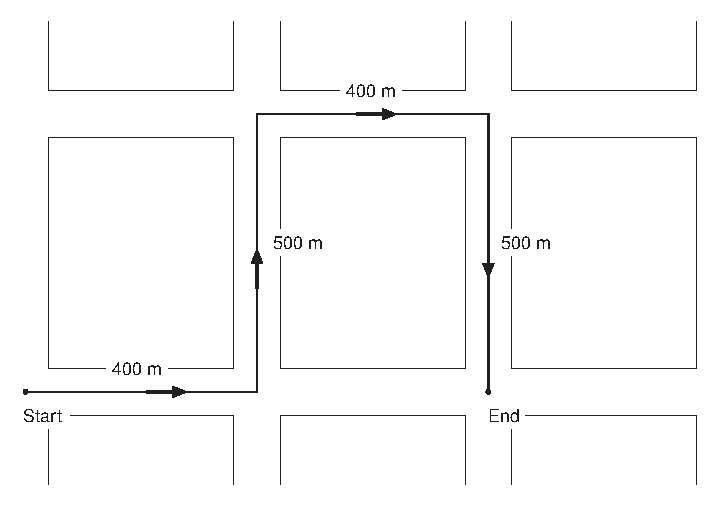
\includegraphics[keepaspectratio,width=\linewidth]{June2000-Q01}
    \end{center}
    What is the magnitude of the total displacement of the school bus from the start to the end of its trip?
    \begin{multicols}{2}
    \begin{choices}
        \wrongchoice{\SI{400}{\meter}}
        \wrongchoice{\SI{500}{\meter}}
      \correctchoice{\SI{800}{\meter}}
        \wrongchoice{\SI{1800}{\meter}}
    \end{choices}
    \end{multicols}
\end{question}
}

\element{nysed}{
\begin{question}{June2000-Q05}
    In the diagram below, a force, $F$, is applied to the handle of a lawnmower inclined at angle $\theta$ to the ground.
    \begin{center}
        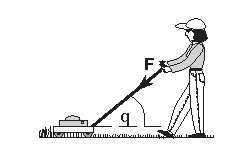
\includegraphics[keepaspectratio,scale=1.0]{June2000-Q05}
    \end{center}
    The magnitude of the horizontal component of force $F$ depends on:
    \begin{choices}
        \wrongchoice{the magnitude of the force $F$, only}
        \wrongchoice{the measure of angle $\theta$, only}
      \correctchoice{both the magnitude of force $F$ and the measure of angle $\theta$.}
        \wrongchoice{neither the magnitude of force $F$ nor the measure of angle $\theta$.}
    \end{choices}
\end{question}
}


\element{nysed}{
\begin{question}{June2000-Q06}
    Equilibrium exists in a system where three forces are acting concurrently on an object.
    If the system includes a \SI{5.0}{\newton} force due north and a \SI{2.0}{\newton} force due south, the third force must be:
    \begin{multicols}{2}
    \begin{choices}
        \wrongchoice{\SI{7.0}{\newton} south}
        \wrongchoice{\SI{7.0}{\newton} north}
      \correctchoice{\SI{3.0}{\newton} south}
        \wrongchoice{\SI{3.0}{\newton} north}
    \end{choices}
    \end{multicols}
\end{question}
}

\element{nysed}{
\begin{question}{June2000-Q09}
    Which term represents a vector quantity and its respective unit?
    \begin{multicols}{2}
    \begin{choices}
        \wrongchoice{weight (\si{\kilo\gram})}
        \wrongchoice{mass (\si{\kilo\gram})}
      \correctchoice{force (\si{\newton})}
        \wrongchoice{momentum (\si{\newton})}
    \end{choices}
    \end{multicols}
\end{question}
}

\element{nysed}{
\begin{question}{June2000-Q10}
    The vector below represents the resultant of two forces acting concurrently on an object at point $P$.
    \begin{center}
    \begin{tikzpicture}
        \draw[fill] (0,0) circle [radius=2pt];
        \node[anchor=west] at (0,0) {$P$};
        \draw[thick,->] (0,0) -- (150:3.00cm);
        \node[anchor=south,rotate=-30] at (150:1.5cm) {Resultant};
    \end{tikzpicture}
    \end{center}
    Which pair of vectors best represents two concurrent forces that combine to produce this resultant force vector?
    \begin{multicols}{2}
    \begin{choices}
        \AMCboxDimensions{down=-1.0cm}
        \correctchoice{
            \begin{tikzpicture}[scale=0.75]
                \draw[draw=white] (-2cm,-1cm) rectangle (2cm,1cm);
                \draw[fill] (0,0) circle [radius=2pt];
                \node[anchor=north] at (0,0) {$P$};
                \draw[thick,->] (0,0) -- (0:1.5cm);
                \draw[thick,->] (0,0) -- (120:1.5cm);
            \end{tikzpicture}
        }
        \wrongchoice{
            \begin{tikzpicture}[scale=0.75]
                \draw[draw=white] (-2cm,-1cm) rectangle (2cm,1.3cm);
                \draw[fill] (0,0) circle [radius=2pt];
                \node[anchor=east] at (0,0) {$P$};
                \draw[thick,->] (0,0) -- (0:2cm);
                \draw[thick,->] (0,0) -- (90:1cm);
            \end{tikzpicture}
        }
        \wrongchoice{
            \begin{tikzpicture}[scale=0.75]
                \draw[draw=white] (-2cm,-1cm) rectangle (2cm,1cm);
                \draw[fill] (0,0) circle [radius=2pt];
                \node[anchor=south] at (0,0) {$P$};
                \draw[thick,->] (0,0) -- (180:2cm);
                \draw[thick,->] (0,0) -- (270:1cm);
            \end{tikzpicture}
        }
        \wrongchoice{
            \begin{tikzpicture}[scale=0.75]
                \draw[draw=white] (-2cm,-1cm) rectangle (2cm,1cm);
                \draw[fill] (0,0) circle [radius=2pt];
                \node[anchor=west] at (0,0) {$P$};
                \draw[thick,->] (0,0) -- (180:1.5cm);
                \draw[thick,->] (0,0) -- (120:1.5cm);
            \end{tikzpicture}
        }
    \end{choices}
    \end{multicols}
\end{question}
}


%% Section June1999
%%--------------------
\element{nysed}{
\begin{question}{June1999-Q01}
    A shown in the diagram below,
        a painter climbs \SI{7.3}{\meter} up a vertical scaffold from $A$ to $B$ and then walks \SI{11}{\meter} from $B$ to $C$ along a level platform.
    \begin{center}
        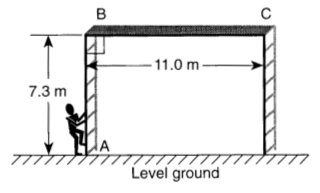
\includegraphics[keepaspectratio,scale=0.80]{June1999-Q01}
    \end{center}
    The magnitude of the painter's total displacement while moving from $A$ to $C$ is:
    \begin{multicols}{2}
    \begin{choices}
        \wrongchoice{\SI{3.7}{\meter}}
      \correctchoice{\SI{13.2}{\meter}}
        \wrongchoice{\SI{18.3}{\meter}}
        \wrongchoice{\SI{25.6}{\meter}}
    \end{choices}
    \end{multicols}
\end{question}
}

\element{nysed}{
\begin{question}{June1999-Q07}
    Which combination of three concurrent forces acting on a body could \emph{not} produce equilibrium?
    \begin{multicols}{2}
    \begin{choices}
      \correctchoice{\SI{1}{\newton},\SI{3}{\newton},\SI{5}{\newton}}
        \wrongchoice{\SI{2}{\newton},\SI{2}{\newton},\SI{2}{\newton}}
        \wrongchoice{\SI{3}{\newton},\SI{4}{\newton},\SI{5}{\newton}}
        \wrongchoice{\SI{4}{\newton},\SI{4}{\newton},\SI{5}{\newton}}
    \end{choices}
    \end{multicols}
\end{question}
}


%% Section June1998
%%--------------------
\element{nysed}{
\begin{question}{June1998-Q01}
    A car travels \SI{12}{\kilo\meter} due north and then \SI{8}{\kilo\meter} due west going from town $A$ to town $B$.
    What is the magnitude of the displacement of a helicopter that flies in a straight line from town $A$ to town $B$?
    \begin{multicols}{2}
    \begin{choices}
        \wrongchoice{\SI{20}{\kilo\meter}}
      \correctchoice{\SI{14}{\kilo\meter}}
        \wrongchoice{\SI{10}{\kilo\meter}}
        \wrongchoice{\SI{4}{\kilo\meter}}
    \end{choices}
    \end{multicols}
\end{question}
}

\element{nysed}{
\begin{question}{June1998-Q04}
    Forces $F_1$ and $F_2$ act concurrently on point $P$,
        as shown in the diagram below.
    \begin{center}
    \begin{tikzpicture}
        \draw[fill] (0,0) circle [radius=2pt];
        \node[anchor=north east] at (0,0) {$P$};

        \draw[thick,->] (0,0) -- (0:3.00cm);
        \node[anchor=north] at (0:1.50cm) {$F_2=\SI{10}{\newton}$ east};

        \draw[thick,->] (0,0) -- (90:3.00cm);
        \node[anchor=south,rotate=90] at (90:1.50cm) {$F_1=\SI{10}{\newton}$ north};
    \end{tikzpicture}
    \end{center}
    The equilibrant of $F_1$ and $F_2$ is:
    \begin{multicols}{2}
    \begin{choices}
      \correctchoice{\SI{14}{\newton} southwest}
        \wrongchoice{\SI{14}{\newton} southeast}
        \wrongchoice{\SI{20}{\newton} southwest}
        \wrongchoice{\SI{20}{\newton} southeast}
    \end{choices}
    \end{multicols}
\end{question}
}

\element{nysed}{
\begin{question}{June1998-Q61}
    An artillery shell is fired at an angle to the horizontal.
    Its initial velocity has a vertical component of \SI{150}{\meter\per\second} and a horizontal component of \SI{260}{\meter\per\second}.
    What is the magnitude of the initial velocity of the shell?
    \begin{multicols}{2}
    \begin{choices}
        \wrongchoice{\SI{9.0e4}{\meter\per\second}}
        \wrongchoice{\SI{4.1e2}{\meter\per\second}}
      \correctchoice{\SI{3.0e2}{\meter\per\second}}
        \wrongchoice{\SI{1.1e2}{\meter\per\second}}
    \end{choices}
    \end{multicols}
\end{question}
}


%% Section June1997
%%--------------------
\element{nysed}{
\begin{question}{June1997-Q01}
    What is the total displacement of a student who walks \num{3} blocks east,
        \num{2} blocks north, and \num{1} block west, and then \num{2} blocks south?
    \begin{multicols}{2}
    \begin{choices}
        \wrongchoice{\num{0}}
      \correctchoice{\num{2} blocks east}
        \wrongchoice{\num{2} blocks west}
        \wrongchoice{\num{8} blocks}
    \end{choices}
    \end{multicols}
\end{question}
}

\element{nysed}{
\begin{question}{June1997-Q08}
    A \SI{100}{\newton} force acts on point $P$,
        as shown in the diagram below.
    \begin{center}
    \begin{tikzpicture}
        \draw[fill] (0,0) circle [radius=2pt];
        \node[anchor=east] at (0,0) {$P$};
        \draw[thick,->] (0,0) -- (0:4.00cm);
        \node[anchor=north] at (0:2.00cm) {Horizontal};
        \draw[thick,->] (0,0) -- (30:4cm);
        \node[anchor=south,rotate=30] at (30:2cm) {\SI{100}{\newton}};
        \draw[thick,->] (0:2cm) arc (0:30:2cm);
        \node[anchor=south west] at (10:2cm) {\ang{30}};
    \end{tikzpicture}
    \end{center}
    The magnitude of the vertical component of this force is approximately:
    \begin{multicols}{2}
    \begin{choices}
        \wrongchoice{\SI{30}{\newton}}
      \correctchoice{\SI{50}{\newton}}
        \wrongchoice{\SI{71}{\newton}}
        \wrongchoice{\SI{87}{\newton}}
    \end{choices}
    \end{multicols}
\end{question}
}

\element{nysed}{
\begin{question}{June1997-Q61}
    A baseball player throws a baseball at a speed of
        \SI{40}{\meter\per\second} at an angle of
        \ang{30} to the ground.
    The horizontal component of the baseball's speed
        is approximately
    \begin{multicols}{2}
    \begin{choices}
        \wrongchoice{\SI{15}{\meter\per\second}}
        \wrongchoice{\SI{20}{\meter\per\second}}
        \wrongchoice{\SI{30}{\meter\per\second}}
      \correctchoice{\SI{35}{\meter\per\second}}
    \end{choices}
    \end{multicols}
\end{question}
}


%% Section June1996
%%--------------------
\element{nysed}{
\begin{question}{June1996-Q02}
    A student walks \SI{40}{\meter} along a hallway that heads due north,
        then turns and walks \SI{30}{\meter} along another hallway that heads due east.
    What is the magnitude of the student's resultant displacement?
    \begin{multicols}{2}
    \begin{choices}
        \wrongchoice{\SI{10}{\meter}}
        \wrongchoice{\SI{35}{\meter}}
      \correctchoice{\SI{50}{\meter}}
        \wrongchoice{\SI{70}{\meter}}
    \end{choices}
    \end{multicols}
\end{question}
}

\element{nysed}{
\begin{question}{June1996-Q08}
    Which pair of concurrent forces could produce a resultant force having a magnitude of \SI{10}{\newton}?
    \begin{multicols}{2}
    \begin{choices}
      \correctchoice{\SI{10}{\newton}, \SI{10}{\newton}}
        \wrongchoice{\SI{10}{\newton}, \SI{30}{\newton}}
        \wrongchoice{\SI{4.7}{\newton}, \SI{4.7}{\newton}}
        \wrongchoice{\SI{4.7}{\newton}, \SI{5.0}{\newton}}
    \end{choices}
    \end{multicols}
\end{question}
}


%% Section June1995
%%--------------------
\element{nysed}{
\begin{question}{June1995-Q06}
    A river flows due east at \SI{1.5}{\meter\per\second}.
    A motorboat leaves the north short of the river and heads due south at \SI{2.0}{\meter\per\second},
        as shown in the diagram below.
    \begin{center}
    \begin{tikzpicture}
        %% Banks
        \draw[ultra thick] (-3,+2) -- (+3,+2);
        \draw[ultra thick] (-3,-2) -- (+3,-2);
        %% Compass
        \node[circle,minimum size=4ex] (C) at (-3,0) {};
        \fill (C.west) to[out=20,in=160] (C.east) to[out=200,in=340] (C.west) -- cycle;
        \fill (C.north) to[out=290,in=70] (C.south) to[out=110,in=250] (C.north) -- cycle;
        %% Compass labels
        \node[anchor=west] at (C.east) {E};
        \node[anchor=east] at (C.west) {W};
        \node[anchor=south] at (C.north) {N};
        \node[anchor=north] at (C.south) {S};
        %% Boat
        \node[minimum size=0.5cm] (B) at (-1.5,1) {};
        \draw[fill=white!90!black] (B.south east) -- ++(225:0.3535) -- (B.south west) -- (B.north west) -- (B.north east) -- cycle;
        \draw[thick,->] (B.south) ++(270:0.25) -- ++(270:1.33)
            node[pos=0.5,anchor=west,text centered,text width=4em] {Boat \SI{2.0}{\meter\per\second}};
        %% Current
        \draw[thick,->] (1.5,0) -- ++(0:1) 
            node[pos=0.5,anchor=south,text centered,text width=4em] {River \SI{1.5}{\meter\per\second}};
    \end{tikzpicture}
    \end{center}
    Which vector best represents the resultant velocity of the boat relative to the riverbank?
    \begin{multicols}{2}
    \begin{choices}
        \AMCboxDimensions{down=-1cm}
        \wrongchoice{
            \begin{tikzpicture}
                \draw[dashed,white!60!black] (-1,0.5) rectangle (2,-2);
                \node[anchor=center] (A) at (0,0) {\SI{2.0}{\meter\per\second}};
                \draw[thick,->] (A.south) -- ++(270:1);
            \end{tikzpicture}
        }
        \wrongchoice{
            \begin{tikzpicture}
                \draw[dashed,white!60!black] (-1,0.5) rectangle (2,-2);
                \node[anchor=center] (A) at (0,0) {\SI{2.0}{\meter\per\second}};
                \draw[thick,->] (A.south) -- ++(315:1);
            \end{tikzpicture}
        }
        \wrongchoice{
            \begin{tikzpicture}
                \draw[dashed,white!60!black] (-1,0.5) rectangle (2,-2);
                \node[anchor=center] (A) at (0,0) {\SI{3.5}{\meter\per\second}};
                \draw[thick,->] (A.south) -- ++(270:1.75);
            \end{tikzpicture}
        }
        \correctchoice{
            \begin{tikzpicture}
                \draw[dashed,white!60!black] (-1,0.5) rectangle (2,-2);
                \node[anchor=center] (A) at (0,0) {\SI{2.5}{\meter\per\second}};
                \draw[thick,->] (A.south) -- ++(315:1.25);
            \end{tikzpicture}
        }
    \end{choices}
    \end{multicols}
\end{question}
}


%% Section June1994
%%--------------------
\element{nysed}{
\begin{question}{June1994-Q01}
    A car travels \SI{20}{\meter} east in \SI{1.0}{\second}.
    The displacement of the car at the end of this \SI{1.0}{\second} interval is:
    \begin{multicols}{2}
    \begin{choices}
        \wrongchoice{\SI{20}{\meter}}
        \wrongchoice{\SI{20}{\meter\per\second}}
      \correctchoice{\SI{20}{\meter} east}
        \wrongchoice{\SI{20}{\meter\per\second} east}
    \end{choices}
    \end{multicols}
\end{question}
}

\element{nysed}{
\begin{question}{June1994-Q04}
    Which is a vector quantity?
    \begin{multicols}{2}
    \begin{choices}
        \wrongchoice{distance}
        \wrongchoice{time}
        \wrongchoice{speed}
      \correctchoice{acceleration}
    \end{choices}
    \end{multicols}
\end{question}
}



%% Section June1990
%%--------------------
\element{nysed}{
\begin{question}{June1990-Q05}
    A student walks 3 blocks south, 4 blocks west, and 3 blocks north.
    What is the displacement of the student?
    \begin{multicols}{2}
    \begin{choices}
        \wrongchoice{10 blocks east}
        \wrongchoice{10 blocks west}
        \wrongchoice{4 blocks east}
      \correctchoice{4 blocks west}
    \end{choices}
    \end{multicols}
\end{question}
}

\element{nysed}{
\begin{question}{June1989-Q08}
    Which vector below represents the resultant of the concurrent vectors $A$ and $B$ in the diagram.
    \begin{center}
    \begin{tikzpicture}
        \draw[thick,-latex] (0,0) -- (1,2) node[pos=0.5,anchor=south east] {$A$};
        \draw[thick,-latex] (0,0) -- (3,1) node[pos=0.5,anchor=north west] {$B$};
    \end{tikzpicture}
    \end{center}
    \begin{multicols}{2}
    \begin{choices}
        \AMCboxDimensions{down=-1.2cm}
        \wrongchoice{
            \begin{tikzpicture}
                \draw[dashed,white!60!black] (-3,-3) rectangle (0,0);
                \draw[thick,-latex] (0,0) -- (-3,-3);
            \end{tikzpicture}
        }
        \wrongchoice{
            \begin{tikzpicture}
                \draw[dashed,white!60!black] (-0.5,1) rectangle (2.5,-2);
                \draw[thick,-latex] (0,0) -- (2,-1);
                %% original was a weak distractor
                %\draw[thick,->] (0,0) -- (0,-3);
            \end{tikzpicture}
        }
        %% ANS is 3
        \correctchoice{
            \begin{tikzpicture}
                \draw[dashed,white!60!black] (0,0) rectangle (3,3);
                \draw[thick,-latex] (0,0) -- (3,3);
            \end{tikzpicture}
        }
        \wrongchoice{
            \begin{tikzpicture}
                \draw[dashed,white!60!black] (-2.5,-1) rectangle (0.5,2);
                \draw[thick,-latex] (0,0) -- (-2,1);
                %% original was a weak distractor
                %\draw[thick,->] (0,0) -- (-0.5,2.5);
            \end{tikzpicture}
        }
    \end{choices}
    \end{multicols}
\end{question}
}


%% Section June1986
%%--------------------
\element{nysed}{
\begin{question}{June1986-Q04}
    A ball is fired with a velocity of \SI{12}{\meter\per\second} from a cannon pointing north,
        while the cannon is moving eastward at a velocity of \SI{24}{\meter\per\second}.
    Which vector best represents the resultant velocity of the ball as it leaves the cannon?
    \begin{multicols}{2}
    \begin{choices}
        %\AMCboxDimensions{down=-1.2cm}
        \AMCboxDimensions{down=-0.8cm}
        \wrongchoice{
            \begin{tikzpicture}
                \draw[dashed,white!60!black] (-1.5,-1.0) rectangle (1.5,1.5);
                \draw[thick,->] (-1.00,0) -- (1.00,0) node[anchor=west] {E};
                \draw[thick,->] (0,-1.00) -- (0,1.00) node[anchor=south] {N};
                \draw[very thick,-latex] (0,0) -- (153:1.5);
            \end{tikzpicture}
        }
        \wrongchoice{
            \begin{tikzpicture}
                \draw[dashed,white!60!black] (-1.5,-1.0) rectangle (1.5,1.5);
                \draw[thick,->] (-1.00,0) -- (1.00,0) node[anchor=west] {E};
                \draw[thick,->] (0,-1.00) -- (0,1.00) node[anchor=south] {N};
                \draw[very thick,-latex] (0,0) -- (116:1.5);
            \end{tikzpicture}
        }
        %% ANS is 3
        \correctchoice{
            \begin{tikzpicture}
                \draw[dashed,white!60!black] (-1.5,-1.0) rectangle (1.5,1.5);
                \draw[thick,->] (-1.00,0) -- (1.00,0) node[anchor=west] {E};
                \draw[thick,->] (0,-1.00) -- (0,1.00) node[anchor=south] {N};
                \draw[very thick,-latex] (0,0) -- (26:1.5);
            \end{tikzpicture}
        }
        \wrongchoice{
            \begin{tikzpicture}
                \draw[dashed,white!60!black] (-1.5,-1.0) rectangle (1.5,1.5);
                \draw[thick,->] (-1.00,0) -- (1.00,0) node[anchor=west] {E};
                \draw[thick,->] (0,-1.00) -- (0,1.00) node[anchor=south] {N};
                \draw[very thick,-latex] (0,0) -- (63:1.5);
            \end{tikzpicture}
        }
    \end{choices}
    \end{multicols}
\end{question}
}



\endinput



%
%% Friction Questions used on the
%% NYSED Physics Regents Examination
%%--------------------------------------------------

%% this section contains 39 problems


%% Section June2014
%%--------------------


%% Section June2013
%%--------------------
\element{nysed}{
\begin{question}{June2013-Q08}
    An \SI{8.0}{\newton} wooden block slides across a horizontal wooden floor at constant velocity.
    What is the magnitude of the force of kinetic friction between the block and the floor?
    %% NOTE: Requies reference to NYSED reference sheet
    \begin{multicols}{2}
    \begin{choices}
      \correctchoice{\SI{2.4}{\newton}}
        \wrongchoice{\SI{3.4}{\newton}}
        \wrongchoice{\SI{8.0}{\newton}}
        \wrongchoice{\SI{27}{\newton}}
    \end{choices}
    \end{multicols}
\end{question}
}

\element{nysed}{
\begin{question}{June2013-Q12}
    An \SI{8.0}{\newton} block is accelerating down a frictionless ramp inclined at \ang{15} to the horizontal,
        as shown in the diagram below.
    \begin{center}\small
    \begin{tikzpicture}
        %% Ramp
        \draw[thick] (0,0) -- (15:6)
            node[pos=0.80,anchor=north,rotate=15] {frictionless ramp};
        \draw[thick,<->,dashed] (0:2) arc (0:15:2)
            node[pos=0.5,anchor=west] {\ang{15}};
        %% Block
        \node[draw,rectangle,minimum size=0.75cm,rotate=15,anchor=south]
            (B) at (15:5) {\SI{8.0}{\newton}};
        \draw[thick,->] (B.west) -- ++ (195:1) node[pos=0.66,anchor=south,rotate=15] {$a$};
        %% Horizontal
        \draw[thick] (0:0) -- (0:5.8)
            node[pos=0.5,anchor=north] {horizontal};
    \end{tikzpicture}
    \end{center}
    What is the magnitude of the net force causing the block's acceleration?
    \begin{multicols}{2}
    \begin{choices}
        \wrongchoice{\SI{0}{\newton}}
      \correctchoice{\SI{2.1}{\newton}}
        \wrongchoice{\SI{7.7}{\newton}}
        \wrongchoice{\SI{8.0}{\newton}}
    \end{choices}
    \end{multicols}
\end{question}
}


%% Section June2012
%%--------------------
\element{nysed}{
\begin{question}{June2012-Q11}
    A \SI{0.50}{\kilo\gram} puck sliding on a horizontal shuffleboard court is slowed to rest by a frictional force of \SI{1.2}{\newton}.
    What is the coefficient of kinetic friction between the puck and the surface of the shuffleboard court?
    \begin{multicols}{2}
    \begin{choices}
      \correctchoice{\num{0.24}}
        \wrongchoice{\num{0.42}}
        \wrongchoice{\num{0.60}}
        \wrongchoice{\num{4.1}}
    \end{choices}
    \end{multicols}
\end{question}
}


%% Section June2011
%%--------------------
\element{nysed}{
\begin{question}{June2011-Q39}
    A child pulls a wagon at a constant velocity along a level sidewalk.
    The child does this by applying a \SI{22}{\newton} force to the wagon handle,
        which is inclined at \ang{35} to the sidewalk as shown below.
    \begin{center}
    \begin{tikzpicture}
        %% ground
        \draw (-4,0) -- (4,0);
        \node[anchor=north,minimum width=8cm,pattern=north east lines] at (0,0) {};
        \node[anchor=north] at (0,-1em) {Level sidewalk};
        %% Cart
        \node[draw,fill=white!90!black,minimum height=1.33cm,minimum width=2cm,anchor=south] (L) at (-1,0.33) {};
        \draw[fill=white] (L.south west) ++(0:0.5) circle (0.33);
        \draw[fill=black] (L.south west) ++(0:0.5) circle (1pt);
        \draw[fill=white] (L.south east) ++(180:0.5) circle (0.33);
        \draw[fill=black] (L.south east) ++(180:0.5) circle (1pt);
        %% vector
        \draw[thick,->] (L.east) -- ++(35:3) node[pos=0.5,anchor=south,rotate=35] {\SI{22}{\newton}};
        \draw[dashed] (L.east) -- ++(0:{3*cos(35)});
        \draw (L.east) ++ (0:1.5) arc(0:35:1.5) node[pos=0.5,anchor=west] {\ang{35}};
    \end{tikzpicture}
    \end{center}
    What is the magnitude of the force of friction on the wagon?
    \begin{multicols}{2}
    \begin{choices}
        \wrongchoice{\SI{11}{\newton}}
        \wrongchoice{\SI{13}{\newton}}
      \correctchoice{\SI{18}{\newton}}
        \wrongchoice{\SI{22}{\newton}}
    \end{choices}
    \end{multicols}
\end{question}
}


%% Section June2010
%%--------------------


%% Section June2009
%%--------------------


%% Section Jan2009
%%--------------------
\element{nysed}{
\begin{question}{Jan2009-Q11}
    Which statement best explains why a ``wet saw'' used to cut through fine optical crystals is constantly lubricated with oil?
    \begin{choices}
      \correctchoice{Lubrication decreases friction and minimizes the increase of internal energy.}
        \wrongchoice{Lubrication decreases friction and maximizes the increase of internal energy.}
        \wrongchoice{Lubrication increases friction and minimizes the increase of internal energy.}
        \wrongchoice{Lubrication increases friction and maximizes the increase of internal energy.}
    \end{choices}
\end{question}
}

\element{nysed}{
\begin{question}{Jan2009-Q37}
    The diagram below shows a \SI{1.0e5}{\newton} truck at rest on a hill that makes an angle of \ang{8.0} with the horizontal.
    \begin{center}
    \pgfdeclarelayer{bg}
    \pgfsetlayers{bg,main}
    \begin{tikzpicture}
        %% incline
        \draw[thick] ({8*cos(8)},0) -- (0,0) -- (8:8);
        \node[anchor=north] at (4,0)  {Horizontal};
        \draw[<->] (6,0) arc (0:8:6) node[pos=0.5,anchor=west] {\ang{8.0}};
        %% Truck
        \begin{pgfonlayer}{main}
            \node[draw,fill=white,minimum size=0.1cm,circle,rotate=8,anchor=south] (W1) at (8:2.5) {};
            \node[draw,fill=white,minimum size=0.1cm,circle,rotate=8,anchor=south] (W2) at (8:3.05) {};
            \node[draw,fill=white,minimum size=0.1cm,circle,rotate=8,anchor=south] (W3) at (8:4.1) {};
            \draw[fill=white!60!black] (W1) circle (1pt);
            \draw[fill=white!60!black] (W2) circle (1pt);
            \draw[fill=white!60!black] (W3) circle (1pt);
        \end{pgfonlayer}
        \begin{pgfonlayer}{bg}
            \node[draw,minimum size=0.5cm,anchor=south,rotate=8,shift={(105:-0.2)}] (R) at (W1.north) {};
            \node[draw,minimum width=1.5cm,minimum height=0.8cm,anchor=south west,rotate=8] at (R.south east) {\SI{e5}{\newton}};
        \end{pgfonlayer}
    \end{tikzpicture}
    \end{center}
    What is the component of the truck’s weight parallel to the hill?
    \begin{multicols}{2}
    \begin{choices}
        \wrongchoice{\SI{1.4e3}{\newton}}
        \wrongchoice{\SI{1.0e4}{\newton}}
      \correctchoice{\SI{1.4e4}{\newton}}
        \wrongchoice{\SI{9.9e4}{\newton}}
    \end{choices}
    \end{multicols}
\end{question}
}


%% Section June2008
%%--------------------
\element{nysed}{
\begin{question}{June2008-Q08}
    A \SI{1200}{\kilo\gram} space vehicle travels at \SI{4.8}{\meter\per\second} along the level surface of Mars.
    If the magnitude of the gravitational field strength on the surface of Mars is \SI{3.7}{\newton\per\kilo\gram},
        the magnitude of the normal force acting on the vehicle is:
    \begin{multicols}{2}
    \begin{choices}
        \wrongchoice{\SI{320}{\newton}}
        \wrongchoice{\SI{930}{\newton}}
      \correctchoice{\SI{4440}{\newton}}
        \wrongchoice{\SI{5800}{\newton}}
    \end{choices}
    \end{multicols}
\end{question}
}

\element{nysed}{
\begin{question}{June2008-Q12}
    An \SI{80}{\kilo\gram} skier slides on waxed skis along a horizontal surface of snow at constant velocity while pushing with his poles.
    What is the horizontal component of the force pushing him forward?
    \begin{multicols}{2}
    \begin{choices}
        \wrongchoice{\SI{0.05}{\newton}}
        \wrongchoice{\SI{0.4}{\newton}}
        \wrongchoice{\SI{40}{\newton}}
      \correctchoice{\SI{4}{\newton}}
    \end{choices}
    \end{multicols}
\end{question}
}

\element{nysed}{
\begin{question}{June2008-Q39}
    A block weighing \SI{10.0}{\newton} is on a ramp inclined at \ang{30.0} to the horizontal.
    A \SI{3.0}{\newton} force of friction, $F_f$,
        acts on the block as it is pulled up the ramp at constant velocity with force $F$,
        which is parallel to the ramp, as shown in the diagram below.
    \begin{center}
    \begin{tikzpicture}
        %% Ground
        \node[anchor=north,fill,pattern=north east lines,minimum width=8cm, minimum height=0.05cm] at (3,0) {};
        \draw (-1,0) -- (7,0);
        %% Incline plane
        \draw[thick] (0,0) -- (30:6);
        \draw[<->] (1.5,0) arc (0:30:1.5) node[pos=0.5,anchor=west] {\ang{30}};
        %% 10 N block
        \node[draw,anchor=south,rotate=30,minimum size=1cm] (A) at (30:3) {\SI{10}{\newton}};
        %% Forces
        \draw[thick,->] (A.west) -- ++(210:1.5) node[pos=0.8,anchor=south,rotate=30] {$F_1=\SI{3.0}{\newton}$};
        \draw[thick,->] (A.east) -- ++(30:3) node[pos=0.5,anchor=south,rotate=30] {$F$};
        %% velocity
        \draw[thick,->] (A.north west) ++(150:1.0) -- ++(30:2) node[pos=0.5,anchor=south,rotate=30] {$v$ (constant)};
    \end{tikzpicture}
    \end{center}
    What is the magnitude of force $F$?
    \begin{multicols}{2}
    \begin{choices}
        \wrongchoice{\SI{7}{\second}}
      \correctchoice{\SI{8}{\second}}
        \wrongchoice{\SI{10}{\second}}
        \wrongchoice{\SI{13}{\second}}
    \end{choices}
    \end{multicols}
\end{question}
}


%% Section Jan2008
%%--------------------
\element{nysed}{
\begin{question}{Jan2008-Q09}
    A car's performance is tested on various horizontal road surfaces.
    The brakes are applied, causing the rubber tires of the car to slide along the road without rolling.
    The tires encounter the greatest force of friction to stop the car on:
    \begin{multicols}{2}
    \begin{choices}
        \wrongchoice{dry concrete}
      \correctchoice{dry asphalt}
        \wrongchoice{wet concrete}
        \wrongchoice{wet asphalt}
    \end{choices}
    \end{multicols}
\end{question}
}


%% Section June2007
%%--------------------


%% Section Jan2007
%%--------------------
\element{nysed}{
\begin{question}{Jan2007-Q38}
    The diagram below shows a \SI{4.0}{\kilo\gram} object accelerating at \SI{10}{\meter\per\second\squared} on a rough horizontal surface.
    \begin{center}
    \begin{tikzpicture}
        %% Block
        \draw[thick] (-1.00,0) rectangle (1.00,1);
        \node[anchor=center] at (0.0,0.5) {$m=\SI{4.0}{\kilo\gram}$};
        %% Floor
        \draw[thick] (-3,0) -- (3,0);
        \foreach \x in {-30,-28,...,30}
            \draw[thin] (\x mm,0cm) -- ++ (220:0.15cm);
        \node[anchor=north] at (0,-0.15) {Frictionless surface};
        %% Force
        \draw[thick,->] (-1.00,0.5) -- (-1.8,0.5)
            node[anchor=south west] {$F_f$};
        \draw[thick,->] (1.00,0.5) -- (5.0,0.5)
            node[above left] {$F=\SI{50}{\newton}$};
        %% Acceleration
        \draw[thick,->] (-2.0,1.5) -- (2.0,1.5)
            node[above left] {Acceleration = \SI{10}{\meter\per\second\squared}};
    \end{tikzpicture}
    \end{center}
    What is the magnitude of the frictional force, $F_f$, acting on the object?
    \begin{multicols}{2}
    \begin{choices}
      \correctchoice{\SI{10}{\newton}}
        \wrongchoice{\SI{5.0}{\newton}}
        \wrongchoice{\SI{20}{\newton}}
        \wrongchoice{\SI{40}{\newton}}
    \end{choices}
    \end{multicols}
\end{question}
}

\element{nysed}{
\begin{question}{Jan2007-Q39}
    What is the magnitude of the force needed to keep a \SI{60}{\newton} rubber block moving across level,
        dry asphalt in a straight line at constant speed of \SI{2.0}{\meter\per\second}?
    \begin{multicols}{2}
    \begin{choices}
      \correctchoice{\SI{40}{\newton}}
        \wrongchoice{\SI{51}{\newton}}
        \wrongchoice{\SI{60}{\newton}}
        \wrongchoice{\SI{120}{\newton}}
    \end{choices}
    \end{multicols}
\end{question}
}


%% Section June2006
%%--------------------


%% Section Jan2006
%%--------------------
\element{nysed}{
\begin{question}{Jan2006-Q10}
    Compared to the force needed to start sliding a crate across a rough level floor,
        the force needed to keep it sliding once it is moving is:
    \begin{multicols}{3}
    \begin{choices}
      \correctchoice{less}
        \wrongchoice{greater}
        \wrongchoice{the same}
    \end{choices}
    \end{multicols}
\end{question}
}

\element{nysed}{
\begin{question}{Jan2006-Q43}
    Which vector diagram best represents a cart slowing down as its travels to the right on a horizontal surface?
    \begin{multicols}{2}
    \begin{choices}
        \AMCboxDimensions{down=-1.3cm}
        \wrongchoice{
            \begin{tikzpicture}
                \draw[dashed,white!90!black] (-1.6,-1.4) rectangle (1.6,1.8);
                %% ground
                \draw[thick] (-1.5,0) -- (1.5,0);
                \node[anchor=north,pattern=north east lines,minimum width=3cm] at (0,0) {};
                %% Cart
                \node[draw,fill=white!90!black,minimum height=0.5cm,minimum width=0.8cm,anchor=south] (L) at (0,0.10) {};
                \draw[fill=white] (L.south west) ++(0:0.15) circle (0.10);
                \draw[fill=black] (L.south west) ++(0:0.15) circle (0.5pt);
                \draw[fill=white] (L.south east) ++(180:0.15) circle (0.10);
                \draw[fill=black] (L.south east) ++(180:0.15) circle (0.5pt);
                %% vectors
                \draw[fill] (L.center) circle (1pt);
                \draw[thick,->] (L.center) -- ++(90:1.5) node[anchor=north east] {$F_N$};
                \draw[thick,->] (L.center) -- ++(0:1.5) node[anchor=south east] {$F$};
                \draw[thick,->] (L.center) -- ++(180:1) node[anchor=south west] {$F_f$};
                \draw[thick,->] (L.center) -- ++(270:1.5) node[anchor=south east] {$F_g$};
            \end{tikzpicture}
        }
        \correctchoice{
            \begin{tikzpicture}
                \draw[dashed,white!90!black] (-1.6,-1.4) rectangle (1.6,1.8);
                %% ground
                \draw[thick] (-1.5,0) -- (1.5,0);
                \node[anchor=north,pattern=north east lines,minimum width=3cm] at (0,0) {};
                %% Cart
                \node[draw,fill=white!90!black,minimum height=0.5cm,minimum width=0.8cm,anchor=south] (L) at (0,0.10) {};
                \draw[fill=white] (L.south west) ++(0:0.15) circle (0.10);
                \draw[fill=black] (L.south west) ++(0:0.15) circle (0.5pt);
                \draw[fill=white] (L.south east) ++(180:0.15) circle (0.10);
                \draw[fill=black] (L.south east) ++(180:0.15) circle (0.5pt);
                %% vectors
                \draw[fill] (L.center) circle (1pt);
                \draw[thick,->] (L.center) -- ++(90:1.5) node[anchor=north east] {$F_N$};
                \draw[thick,->] (L.center) -- ++(0:1) node[anchor=south east] {$F$};
                \draw[thick,->] (L.center) -- ++(180:1.5) node[anchor=south west] {$F_f$};
                \draw[thick,->] (L.center) -- ++(270:1.5) node[anchor=south east] {$F_g$};
            \end{tikzpicture}
        }
        \wrongchoice{
            \begin{tikzpicture}
                \draw[dashed,white!90!black] (-1.6,-1.4) rectangle (1.6,1.8);
                %% ground
                \draw[thick] (-1.5,0) -- (1.5,0);
                \node[anchor=north,pattern=north east lines,minimum width=3cm] at (0,0) {};
                %% Cart
                \node[draw,fill=white!90!black,minimum height=0.5cm,minimum width=0.8cm,anchor=south] (L) at (0,0.10) {};
                \draw[fill=white] (L.south west) ++(0:0.15) circle (0.10);
                \draw[fill=black] (L.south west) ++(0:0.15) circle (0.5pt);
                \draw[fill=white] (L.south east) ++(180:0.15) circle (0.10);
                \draw[fill=black] (L.south east) ++(180:0.15) circle (0.5pt);
                %% vectors
                \draw[fill] (L.center) circle (1pt);
                \draw[thick,->] (L.center) -- ++(90:1.5) node[anchor=north east] {$F_N$};
                \draw[thick,->] (L.center) -- ++(0:1) node[anchor=south east] {$F$};
                \draw[thick,->] (L.center) -- ++(180:1) node[anchor=south west] {$F_f$};
                \draw[thick,->] (L.center) -- ++(270:1.5) node[anchor=south east] {$F_g$};
            \end{tikzpicture}
        }
        \wrongchoice{
            \begin{tikzpicture}
                \draw[dashed,white!90!black] (-1.6,-1.4) rectangle (1.6,1.8);
                %% ground
                \draw[thick] (-1.5,0) -- (1.5,0);
                \node[anchor=north,pattern=north east lines,minimum width=3cm] at (0,0) {};
                %% Cart
                \node[draw,fill=white!90!black,minimum height=0.5cm,minimum width=0.8cm,anchor=south] (L) at (0,0.10) {};
                \draw[fill=white] (L.south west) ++(0:0.15) circle (0.10);
                \draw[fill=black] (L.south west) ++(0:0.15) circle (0.5pt);
                \draw[fill=white] (L.south east) ++(180:0.15) circle (0.10);
                \draw[fill=black] (L.south east) ++(180:0.15) circle (0.5pt);
                %% vectors
                \draw[fill] (L.center) circle (1pt);
                \draw[thick,->] (L.center) -- ++(90:1.5) node[anchor=north east] {$F_N$};
                \draw[thick,->] (L.center) -- ++(0:1.5) node[anchor=south east] {$F$};
                \draw[thick,->] (L.center) -- ++(180:1.5) node[anchor=south west] {$F_f$};
                \draw[thick,->] (L.center) -- ++(270:1.5) node[anchor=south east] {$F_g$};
            \end{tikzpicture}
        }
    \end{choices}
    \end{multicols}
\end{question}
}


%% Section June2005
%%--------------------
\element{nysed}{
\begin{question}{June2005-Q13}
    The diagram below shows a \SI{5.00}{\kilo\gram} block at rest on a horizontal, frictionless table.
    \begin{center}
    \begin{tikzpicture}
        %% legs
        \draw (-2,-0.2,-4) rectangle (-1.8,-2,-4);
        \draw (+2,-0.2,-4) rectangle (+1.8,-2,-4);
        \draw (-2,-0.2,+2) rectangle (-1.8,-2,+2);
        \draw (+2,-0.2,+2) rectangle (+1.8,-2,+2);
        %% table
        \draw[fill=white] (-2,0,2) -- (-2,0,-4) -- (2,0,-4) -- (2,0,2) -- cycle;
        \draw (-2,0,2) -- (-2,-0.2,2) -- (2,-0.2,2) -- (2,0,2) -- cycle;
        \draw[fill=white!90!black] (2,0,2) -- (2,0,-4) -- (2,-0.2,-4) -- (2,-0.2,2) -- cycle;
        \node[anchor=north] at (0,-0.2,2) {Table};
        %% 5 kg block
        \draw[fill=white] (-1,0,0) -- (1,0,0) -- (1,2,0) -- (-1,2,0) -- cycle;
        \node[anchor=center,text centered,text width=3em] at (0,1,0) {\SI{5.00}{\kilo\gram} block};
        \draw[fill=white] (-1,2,0) -- (-1,2,-2) -- (1,2,-2) -- (1,2,0)  -- cycle;
        \draw[fill=white!90!black] (1,0,0) -- (1,0,-2) -- (1,2,-2) -- (1,2,0) -- cycle; 
    \end{tikzpicture}
    \end{center}
    Which diagram best represents the force exerted on the block by the table?
    \begin{multicols}{2}
    \begin{choices}\small
        \AMCboxDimensions{down=-1.2cm}
        \correctchoice{
            \begin{tikzpicture}
                \draw[dashed,white!60!black] (-1.5,-1.5) rectangle (1,1.5);
                \node[draw,thick,rectangle,anchor=center,minimum size=2em] (B) at (0,0) {Block};
                \draw[thick,->] (B.north) -- ++(90:1)
                    node[pos=0.5,anchor=east] {\SI{49.1}{\newton}};
            \end{tikzpicture}
        }
        \wrongchoice{
            \begin{tikzpicture}
                \draw[dashed,white!60!black] (-1.5,-1.5) rectangle (1,1.5);
                \node[draw,thick,rectangle,anchor=center,minimum size=2em] (B) at (0,0) {Block};
                \draw[thick,->] (B.south) -- ++(270:1)
                    node[pos=0.5,anchor=east] {\SI{5.00}{\newton}};
            \end{tikzpicture}
        }
        \wrongchoice{
            \begin{tikzpicture}
                \draw[dashed,white!60!black] (-1.5,-1.5) rectangle (1,1.5);
                \node[draw,thick,rectangle,anchor=center,minimum size=2em] (B) at (0,0) {Block};
                \draw[thick,->] (B.north) -- ++(90:1)
                    node[pos=0.5,anchor=east] {\SI{5.00}{\kilo\gram}};
            \end{tikzpicture}
        }
        \wrongchoice{
            \begin{tikzpicture}
                \draw[dashed,white!60!black] (-1.5,-1.5) rectangle (1,1.5);
                \node[draw,thick,rectangle,anchor=center,minimum size=2em] (B) at (0,0) {Block};
                \draw[thick,->] (B.south) -- ++(270:1)
                    node[pos=0.5,anchor=east] {\SI{49.1}{\kilo\gram}};
            \end{tikzpicture}
        }
    \end{choices}
    \end{multicols}
\end{question}
}

\element{nysed}{
\begin{question}{June2005-Q45}
    The diagram below represents a block at rest on an incline.
    \begin{center}
    \begin{tikzpicture}[scale=1.33]
        \node[draw,minimum size=1cm,rotate=30,anchor=south] at (30:3) {Block};
        \draw[thick] (0,0) -- (30:4) -- ++(270:{4*sin(30)});
        %% Floor
        \draw[thick] (-1,0) -- (4,0) node[pos=0.5,anchor=north,yshift=-1em] {Horizontal};
        \node[anchor=north,pattern=north east lines,minimum width=6.65cm] at (1.5,0) {};
    \end{tikzpicture}
    \end{center}
    Which diagram best represents the forces acting on the block?
    ($F_f =\text{frictional force}$, $F_N=\text{normal force}$, and $F_w=\text{weight}$.)
    \begin{multicols}{2}
    \begin{choices}
        \AMCboxDimensions{down=-1.25cm}
        \correctchoice{
            \begin{tikzpicture}
                \draw[dashed,white!60!black] (-1.5,-1.5) rectangle (1.5,1.5);
                \draw[thick,->] (0,0) -- (120:1) node[anchor=south east] {$F_N$};
                \draw[thick,->] (0,0) -- (30:1)  node[anchor=south west] {$F_f$};
                \draw[thick,->] (0,0) -- (270:1) node[anchor=north] {$F_w$};
            \end{tikzpicture}
        }
        \wrongchoice{
            \begin{tikzpicture}
                \draw[dashed,white!60!black] (-1.5,-1.5) rectangle (1.5,1.5);
                \draw[thick,->] (0,0) -- (210:1) node[anchor=north east] {$F_N$};
                \draw[thick,->] (0,0) -- (30:1)  node[anchor=south west] {$F_f$};
                \draw[thick,->] (0,0) -- (300:1) node[anchor=north west] {$F_w$};
            \end{tikzpicture}
        }
        \wrongchoice{
            \begin{tikzpicture}
                \draw[dashed,white!60!black] (-1.5,-1.5) rectangle (1.5,1.5);
                \draw[thick,->] (0,0) -- (90:1)  node[anchor=south] {$F_N$};
                \draw[thick,->] (0,0) -- (210:1) node[anchor=north east] {$F_f$};
                \draw[thick,->] (0,0) -- (330:1) node[anchor=north west] {$F_w$};
            \end{tikzpicture}
        }
        \wrongchoice{
            \begin{tikzpicture}
                \draw[dashed,white!60!black] (-1.5,-1.5) rectangle (1.5,1.5);
                \draw[thick,->] (0,0) -- (30:1)  node[anchor=south west] {$F_N$};
                \draw[thick,->] (0,0) -- (210:1) node[anchor=north east] {$F_f$};
                \draw[thick,->] (0,0) -- (270:1) node[anchor=north] {$F_w$};
            \end{tikzpicture}
        }
    \end{choices}
    \end{multicols}
\end{question}
}


%% Section Jan2005
%%--------------------
\element{nysed}{
\begin{question}{Jan2005-Q09}
    The diagram below shows a sled and rider sliding down a snow covered hill that makes an angle of \ang{30} with the horizontal.
    \begin{center}
    \begin{tikzpicture}[scale=1.33]
        \draw[thick] (0,0) -- (4,0) node[anchor=north,pos=0.5] {Horizontal};
        \node[draw,minimum size=1em,rotate=30,anchor=south] at (30:3) {Sled};
        \draw[thick] (0,0) -- (30:4);
        \draw[thick,->] (0:2) arc(0:30:2) node[pos=0.5,anchor=west] {\ang{30}};
    \end{tikzpicture}
    \end{center}
    Which vector best represents the direction of the normal force, $F_N$, exerted by the hill on the sled?
    \begin{multicols}{2}
    \begin{choices}\small
        \AMCboxDimensions{down=-1.40cm}
        \correctchoice{
            \begin{tikzpicture}[scale=0.75]
                \draw[dashed,white!60!black] (1em,-2em) rectangle (-3cm-1em,3cm);
                \draw (0,0) -- (-3,0)
                    node[pos=0.5,anchor=north] {horizontal};
                \draw[thick,->] (0,0) -- ++(120:3)
                    node[pos=0.5,anchor=south west] {$F_N$};
                \draw[dashed,thick,<->] (120:1.5) arc (120:180:1.5)
                    node[pos=0.5,anchor=east] {\ang{60}};
            \end{tikzpicture}
        }
        \wrongchoice{
            \begin{tikzpicture}[scale=0.75]
                \draw[dashed,white!60!black] (-1em,2em) rectangle (3cm+1em,-3cm);
                \draw (0,0) -- (3,0)
                    node[pos=0.5,anchor=south] {horizontal};
                \draw[thick,->] (0,0) -- ++(300:3)
                    node[pos=0.5,anchor=north east] {$F_N$};
                \draw[dashed,thick,<->] (300:1.5) arc (300:360:1.5)
                    node[pos=0.5,anchor=north west] {\ang{60}};
            \end{tikzpicture}
        }
        \wrongchoice{
            \begin{tikzpicture}[scale=0.75]
                \draw[dashed,white!60!black] (1em,+2em) rectangle (-3cm-1em,-3cm);
                \draw (0,0) -- (-3,0)
                    node[pos=0.5,anchor=south] {horizontal};
                \draw[thick,->] (0,0) -- ++(210:3)
                    node[pos=0.5,anchor=north west] {$F_N$};
                \draw[dashed,thick,<->] (180:1.5) arc (180:210:1.5)
                    node[pos=0.5,anchor=east] {\ang{30}};
            \end{tikzpicture}
        }
        \wrongchoice{
            \begin{tikzpicture}[scale=0.75]
                \draw[dashed,white!60!black] (-1em,-2em) rectangle (3cm+1em,3cm);
                \draw (0,0) -- (3,0)
                    node[pos=0.5,anchor=north] {horizontal};
                \draw[thick,->] (0,0) -- ++(30:3)
                    node[pos=0.5,anchor=south east] {$F_N$};
                \draw[dashed,thick,<->] (0:1.5) arc (0:30:1.5)
                    node[pos=0.5,anchor=west] {\ang{30}};
            \end{tikzpicture}
        }
    \end{choices}
    \end{multicols}
\end{question}
}


%% Section June2004
%%--------------------
\element{nysed}{
\begin{question}{June2004-Q08}
    The force required to start an object sliding across a uniform horizontal surface is larger than the force required to keep the object sliding at a constant velocity.
    The magnitudes of the required forces are different in these situations because the force of kinetic friction:
    \begin{choices}
      \correctchoice{is less than the force of static friction}
        \wrongchoice{is greater than the force of static friction}
        \wrongchoice{increases as the speed of the object relative to the surface increases}
        \wrongchoice{decreases as the speed of the object relative to the surface increases}
    \end{choices}
\end{question}
}


%% Section Jan2004
%%--------------------
\element{nysed}{
\begin{question}{Jan2004-Q10}
    A box is pushed toward the right across a classroom floor.
    The force of friction on the box is directed toward the:
    \begin{multicols}{2}
    \begin{choices}
      \correctchoice{left}
        \wrongchoice{right}
        \wrongchoice{ceiling}
        \wrongchoice{floor}
    \end{choices}
    \end{multicols}
\end{question}
}


%% Section June2003
%%--------------------
\element{nysed}{
\begin{question}{June2003-Q47}
    Three forces act on a box on an inclined plane as shown in the diagram below.
    Vectors are not drawn to scale.
    \begin{center}
    \begin{tikzpicture}
        %% Ramp and floor
        \draw[thick] (0,0) -- (20:6);
        \draw[thick] (0:0) -- (0:5.7)
            node[pos=1.0,anchor=north east] {horizontal};
        %% Block
        \node[draw,rectangle,minimum size=0.75cm,rotate=20,anchor=south west]
            (B) at (20:3) {};
        %% Three Forces
        \draw[thick,->] (B.north) -- ++(110:1)
            node[pos=1.0,anchor=south] {normal force};
        \draw[thick,->] (B.center) -- ++(270:1)
            node[pos=1.0,anchor=north] {weight};
        \draw[thick,->] (B.east) -- ++(20:1)
            node[pos=1.0,anchor=south] {friction};
    \end{tikzpicture}
    \end{center}
    If the box is at rest,
        the net force acting on it is equal to:
    \begin{multicols}{2}
    \begin{choices}
      \correctchoice{zero}
        \wrongchoice{the weight}
        \wrongchoice{friction}
        \wrongchoice{the normal force}
    \end{choices}
    \end{multicols}
\end{question}
}


%% Section Jan2003
%%--------------------
\element{nysed}{
\begin{question}{Jan2003-Q11}
    The diagram below shows a block sliding down a plane inclined at angle $\theta$ with the horizontal.
    \begin{center}
    \begin{tikzpicture}
        %% Plane with Box
        \node[draw,minimum size=1cm,rotate=30,anchor=south] at (30:3) {};
        \draw[thick] (0,0) -- (30:4);
        \draw[dashed,thick,<->] (0:2) arc(0:30:2) node[pos=0.5,anchor=west] {$\theta$};
        %% Floor
        \draw[thick] (0,0) -- (4,0);
        \node[pattern=north east lines,anchor=north,minimum width=4cm] at (2,0) {};
    \end{tikzpicture}
    \end{center}
    As angle $\theta$ is increased,
        the coefficient of kinetic friction between the bottom surface of the block and the surface of the incline will:
    \begin{choices}
      \correctchoice{decrease}
        \wrongchoice{increase}
        \wrongchoice{remain the same}
    \end{choices}
\end{question}
}


%% Section Aug2002
%%--------------------
\element{nysed}{
\begin{question}{Aug2002-Q05}
    In the diagram below, a box is at rest on an inclined plane.
    \begin{center}
    \begin{tikzpicture}
        %% Ramp
        \draw[thick] (0,0) -- (30:5cm);
        \draw[dashed] (0,0) -- (4.3,0)
            node[pos=0.5,anchor=north] {Horizontal};
        %% Block
        \node[thick,draw,rectangle,minimum size=0.66cm,rotate=30,anchor=south] 
            (B) at (30:3cm) {};
        \draw[thick,->] (B) -- ++ (210:1.5cm)
            node[anchor=south west,rotate=30] {$A$};
        \draw[thick,->] (B) -- ++ (30:1.5cm)
            node[anchor=south east,rotate=30] {$B$};
        \draw[thick,->] (30:3cm) +(120:0.33cm) -- ++ (270:0.75cm)
            node[anchor=north] {$C$};
        \draw[thick,->] (30:3cm) +(120:0.33cm) -- ++ (120:1.25cm)
            node[anchor=south,rotate=30] {$D$};
    \end{tikzpicture}
    \end{center}
    Which vector best represents the direction of the normal force acting on the box?
    \begin{multicols}{4}
    \begin{choices}[o]
        \wrongchoice{$A$}
        \wrongchoice{$B$}
      \correctchoice{$C$}
        \wrongchoice{$D$}
    \end{choices}
    \end{multicols}
\end{question}
}

\element{nysed}{
\begin{question}{Aug2002-Q08}
    A block weighing \SI{15}{\newton} is pulled to the top of an incline that is \SI{0.20}{\meter} above the ground, as shown below.
    \begin{center}
    \begin{tikzpicture}
        %% Ramp 5cm wide
        \draw[thick] (0,0) -- (30:5cm);
        \draw[dashed] (-1,0) -- (5,0);
        \draw[thick] (4.4,0.0) -- (4.6,0.0);
        \draw[thick] (4.4,2.5) -- (4.6,2.5);
        \draw[thick,<->] (4.5,0) -- (4.5,2.5)
            node[fill=white,pos=0.5,anchor=center] {\SI{0.20}{\meter}};
        %% Block
        \node[thick,draw,rectangle,minimum width=1cm,minimum height=0.5cm,rotate=30,anchor=south] 
            (B) at (30:3cm) {\SI{15}{\newton}};
        \draw[thick,->] (B) -- ++ (30:1cm);
    \end{tikzpicture}
    \end{center}
    If \SI{4.0}{\joule} of work are needed to pull the block the full length of the incline,
        how much work is done against friction?
    \begin{multicols}{2}
    \begin{choices}
      \correctchoice{\SI{1.0}{\joule}}
        \wrongchoice{\SI{0.0}{\joule}}
        \wrongchoice{\SI{3.0}{\joule}}
        \wrongchoice{\SI{7.0}{\joule}}
    \end{choices}
    \end{multicols}
\end{question}
}

\element{nysed}{
\begin{question}{Aug2002-Q37}
    The diagram below shows a \SI{10.0}{\kilo\gram} mass held at rest on a frictionless \ang{30.0} incline by force $F$.
    \begin{center}
    \begin{tikzpicture}
        %% Ramp
        \draw[thick] (0,0) -- (5.00,2.89) -- (5.00,0.0) -- cycle;
        \draw[thick,dashed,<->] (0:2.0) arc (0:30:2.0)
            node[pos=0.5,anchor=west] {\ang{30}};
        %% Block
        \node[thick,draw,rectangle,minimum size=0.75cm,rotate=30,anchor=south] 
            (B) at (30:2cm) {\SI{10}{\kilo\gram}};
        \draw[thick,->] (B) -- ++ (30:2cm)
            node[pos=0.5,anchor=south,rotate=30] {$F$};
    \end{tikzpicture}
    \end{center}
    What is the approximate magnitude of force $F$?
    \begin{multicols}{2}
    \begin{choices}
        \wrongchoice{\SI{9.81}{\newton}}
      \correctchoice{\SI{49.1}{\newton}}
        \wrongchoice{\SI{85.0}{\newton}}
        \wrongchoice{\SI{98.1}{\newton}}
    \end{choices}
    \end{multicols}
\end{question}
}


%% Section June2002
%%--------------------
\element{nysed}{
\begin{question}{June2002-Q02}
    The diagram below shows a granite block being slide at constant speed across a horizontal concrete floor by a force parallel to the floor.
    \begin{center}
        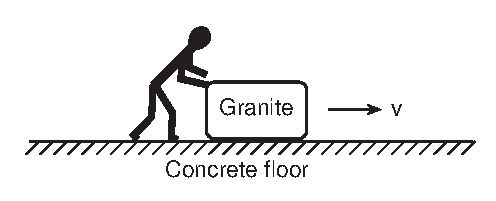
\includegraphics[keepaspectratio,scale=0.9]{June2002-Q02}
    \end{center}
    Which pair of quantities could be used to determine the coefficient of friction for the granite on the concrete?
    \begin{choices}
        \wrongchoice{mass and speed of the block}
        \wrongchoice{mass and normal force on the block}
        \wrongchoice{frictional force and speed of the block}
      \correctchoice{frictional force and normal force on the block}
    \end{choices}
\end{question}
}

%% Section Jan2002
%%--------------------
\element{nysed}{
\begin{question}{Jan2002-Q12}
    The table below lists the coefficients of kinetic friction for four materials sliding over steel.
    \begin{center}
    \begin{tabu}{X[c]X[c]}
        \toprule
        Material & Coefficient of Kinetic Friction \\
        \midrule
        aluminum    & 0.47 \\
        brass       & 0.44 \\
        copper      & 0.36 \\
        steel       & 0.57 \\
        \bottomrule
    \end{tabu}
    \end{center}
    A \SI{10}{\kilo\gram} block of each of these materials is pulled horizontally across a steel floor at constant velocity.
    Which block requires the \emph{smallest} applied force to keep it moving at constant velocity?
    \begin{multicols}{2}
    \begin{choices}
        \wrongchoice{aluminum}
        \wrongchoice{brass}
      \correctchoice{copper}
        \wrongchoice{steel}
    \end{choices}
    \end{multicols}
\end{question}
}


%% Section June2001
%%--------------------
\element{nysed}{
\begin{question}{June2001-Q10}
    A \SI{50}{\newton} horizontal force is needed to keep an object weighing \SI{500}{\newton} moving at a constant velocity of \SI{2.0}{\meter\per\second} across a horizontal surface.
    The magnitude of the frictional force acting on the object is:
    \begin{multicols}{2}
    \begin{choices}
      \correctchoice{\SI{500}{\newton}}
        \wrongchoice{\SI{450}{\newton}}
        \wrongchoice{\SI{50}{\newton}}
        \wrongchoice{\SI{0}{\newton}}
    \end{choices}
    \end{multicols}
\end{question}
}

\element{nysed}{
\begin{question}{June2001-Q11}
    The diagram below represents a block sliding down an incline.
    \begin{center}
    \begin{tikzpicture}[scale=0.8]
        %% Ramp
        \draw[thick] (0,0) -- (30:5cm);
        \draw[dashed] (0,0) -- (4.3,0)
            node[pos=0.5,anchor=north] {Horizontal};
        %% Block
        \node[thick,draw,rectangle,minimum size=1.00cm,rotate=30,anchor=south] (B) at (30:3cm) {};
        %% Vectors
        \draw[thick,->] (B) --++ (120:1.5cm)
            node[anchor=south] {$A$};
        \draw[thick,->] (B) --++ (30:1.5cm)
            node[anchor=west] {$B$};
        \draw[thick,->] (B) --++ (-60:1.5cm)
            node[anchor=north] {$C$};
        \draw[thick,->] (B) --++ (210:1.5cm)
            node[anchor=east] {$D$};
    \end{tikzpicture}
    \end{center}
    Which vector best represents the frictional force acting on the block?
    \begin{multicols}{4}
    \begin{choices}[o]
        \wrongchoice{$A$}
      \correctchoice{$B$}
        \wrongchoice{$C$}
        \wrongchoice{$D$}
    \end{choices}
    \end{multicols}
\end{question}
}

\element{nysed}{
\begin{question}{June2001-Q12}
    A different force is applied to each of four \SI{1}{\kilo\gram} blocks to slide them across a uniform steel surface at constant speed as shown below.
    In which diagram is the coefficient of friction between the block and steel \emph{smallest}?
    \begin{multicols}{2}
    \begin{choices}
        \AMCboxDimensions{down=-0.50cm}
        \correctchoice{
            \begin{tikzpicture}[font=\footnotesize,xscale=0.66]
                %% Force
                \draw[thick,->] (-2,0.5) -- (0,0.5)
                    node[pos=1.0,anchor=south east] {$F=\SI{2}{\newton}$};
                %% Block
                \draw[thick] (0,0) rectangle (2,1);
                \node[anchor=center,text width=3em,text centered]
                    at (1,0.5) {\SI{1}{\kilo\gram} Block};
                %% Floor
                \draw[thick] (-2,0) -- (2.5,0);
                \node[anchor=north,minimum width=3cm,pattern=north east lines] at (0.25,0) {};
                \node[anchor=north] at (0,-0.2) {Steel};
            \end{tikzpicture}
        }
        \wrongchoice{
            \begin{tikzpicture}[font=\footnotesize,xscale=0.66]
                %% Force
                \draw[thick,->] (-2,0.5) -- (0,0.5)
                    node[pos=1.0,anchor=south east] {$F=\SI{5}{\newton}$};
                %% Block
                \draw[thick] (0,0) rectangle (2,1);
                \draw[thick] (0,0) rectangle (2,1);
                \node[anchor=center,text width=3em,text centered]
                    at (1,0.5) {\SI{1}{\kilo\gram} Block};
                %% Floor
                \draw[thick] (-2,0) -- (2.5,0);
                \node[anchor=north,minimum width=3cm,pattern=north east lines] at (0.25,0) {};
                \node[anchor=north] at (0,-0.2) {Steel};
            \end{tikzpicture}
        }
        \wrongchoice{
            \begin{tikzpicture}[font=\footnotesize,xscale=0.66]
                %% Force
                \draw[thick,->] (-2,0.5) -- (0,0.5)
                    node[pos=1.0,anchor=south east] {$F=\SI{3}{\newton}$};
                %% Block
                \draw[thick] (0,0) rectangle (2,1);
                \node[anchor=center,text width=3em,text centered]
                    at (1,0.5) {\SI{1}{\kilo\gram} Block};
                %% Floor
                \draw[thick] (-2,0) -- (2.5,0);
                \node[anchor=north,minimum width=3cm,pattern=north east lines] at (0.25,0) {};
                \node[anchor=north] at (0,-0.2) {Steel};
            \end{tikzpicture}
        }
        \wrongchoice{
            \begin{tikzpicture}[font=\footnotesize,xscale=0.66]
                %% Force
                \draw[thick,->] (-2,0.5) -- (0,0.5)
                    node[pos=1.0,anchor=south east] {$F=\SI{4}{\newton}$};
                %% Block
                \draw[thick] (0,0) rectangle (2,1);
                \node[anchor=center,text width=3em,text centered]
                    at (1,0.5) {\SI{1}{\kilo\gram} Block};
                %% Floor
                \draw[thick] (-2,0) -- (2.5,0);
                \node[anchor=north,minimum width=3cm,pattern=north east lines] at (0.25,0) {};
                \node[anchor=north] at (0,-0.2) {Steel};
            \end{tikzpicture}
        }
    \end{choices}
    \end{multicols}
\end{question}
}


%% Section Jan2001
%%--------------------
\element{nysed}{
\begin{question}{Jan2001-Q15}
    A wooden block is at rest on a horizontal steel surface.
    If a \SI{10}{\newton} force applied parallel to the surface is required to set the block in motion,
        how much force is required to keep the block moving at constant velocity?
    \begin{choices}
        \wrongchoice{less than \SI{10}{\newton}}
        \wrongchoice{greater than \SI{10}{\newton}}
      \correctchoice{\SI{10}{\newton}}
    \end{choices}
\end{question}
}


%% Section June2000
%%--------------------
\element{nysed}{
\begin{question}{June2000-Q04}
    A cart moving across a level surface accelerates uniformly at \SI{1.0}{\meter\per\second\squared}.
    What additional information is required to determine the distance traveled by the cart during this \SI{2.0}{\second} interval?
    \begin{choices}
        \wrongchoice{coefficient of friction between the cart and the surface}
        \wrongchoice{mass of the cart}
        \wrongchoice{net force acting on the cart}
      \correctchoice{initial velocity of the cart}
    \end{choices}
\end{question}
}

\element{nysed}{
\begin{question}{June2000-Q14}
    Sand is often placed on an icy road because the sand:
    \begin{choices}
        \wrongchoice{decreases the coefficient of friction between the tire and the road}
      \correctchoice{increases the coefficient of friction between the tire and the road}
        \wrongchoice{decreases the gravitational force on the car}
        \wrongchoice{increases the normal force of a car on the road}
    \end{choices}
\end{question}
}



%% Section June1999
%%--------------------
\element{nysed}{
\begin{question}{June1999-Q08}
    If a \SI{30}{\newton} force is required to accelerate a \SI{2}{\kilo\gram} object at \SI{10}{\meter\per\second},
        over a level floor, then the magnitude of the frictional force acting on the object is:
    \begin{multicols}{2}
    \begin{choices}
        \wrongchoice{\SI{0}{\newton}}
      \correctchoice{\SI{10}{\newton}}
        \wrongchoice{\SI{20}{\newton}}
        \wrongchoice{\SI{30}{\newton}}
    \end{choices}
    \end{multicols}
\end{question}
}

\element{nysed}{
\begin{question}{June1999-Q09}
    The diagram below shows a stuent applying a \SI{10}{\newton} force to slide a piece of wood at constant speed across a horizontal surface.
    After the wood is cut in half, one piece is placed on top of the other, as shown.
    \begin{center}
    \begin{tikzpicture}
        %% NOTE: TODO: draw tikz
        %% 3d cube??
        %% rectangle object and make 3d??
        \begin{scope}[xshift=-2cm]
        \end{scope}
    \end{tikzpicture}
    \end{center}
    What is the magnitude of the force, $F$,
        required to slide the stacked wood at constant speed across the surface?
    \begin{multicols}{2}
    \begin{choices}
        \wrongchoice{\SI{40}{\newton}}
        \wrongchoice{\SI{20}{\newton}}
      \correctchoice{\SI{10}{\newton}}
        \wrongchoice{\SI{5.0}{\newton}}
    \end{choices}
    \end{multicols}
\end{question}
}

\element{nysed}{
\begin{question}{June1999-Q10}
    In the diagram below, a block rests on a ramp,
        making an angle $\theta$ with the horizontal.
    \begin{center}
    \begin{tikzpicture}
        %% ramp
        \draw ({5*cos(30)},0) -- (0,0) -- (30:5);
        \draw (1,0) arc (0:30:1) node[pos=0.5,anchor=west] {$\theta$};
        %% block
        \node[draw,anchor=south,rotate=30,minimum size=1cm] at (30:3) {Block};
    \end{tikzpicture}
    \end{center}
    If angle $\theta$ is increased, what will occur?
    \begin{choices}
        \wrongchoice{The block's mass will decrease.}
        \wrongchoice{The block's weight will increase.}
        \wrongchoice{The block's component of weight parallel to the ramp will decrease.}
      \correctchoice{The block's component of weight parallel to the ramp will increase.}
    \end{choices}
\end{question}
}


%% Section June1998
%%--------------------
\element{nysed}{
\begin{question}{June1998-Q06}
    A \SI{1.0}{\kilo\gram} block is placed on each of four frictionless planes inclined at different angles.
    On which inclined plane will the acceleration of the block be greatest?
    \begin{multicols}{2}
    \begin{choices} \small
        \AMCboxDimensions{down=-0.5cm}
        \wrongchoice{
            \begin{tikzpicture}[scale=0.9]
                \draw[dashed] (-0.2,-0.5) rectangle (3.2,2.5);
                \draw (0,0) -- (0,1) -- (3,0) -- cycle;
                \node[anchor=north] at (1.5,0) {\SI{3.0}{\meter}};
                \node[anchor=west] at (0,0.25) {\SI{1.0}{\meter}};
                \node[draw,anchor=south,rotate=-18.43,minimum size=1cm] at (1,0.66) {\SI{1.0}{\kilo\gram}};
            \end{tikzpicture}
        }
        \wrongchoice{
            \begin{tikzpicture}[scale=0.9]
                \draw[dashed] (-1.2,-0.5) rectangle (2.2,2.5);
                \draw (0,0) -- (0,1) -- (2,0) -- cycle;
                \node[anchor=north] at (1,0) {\SI{2.0}{\meter}};
                \node[anchor=east] at (0,0.5) {\SI{1.0}{\meter}};
                \node[draw,anchor=south,rotate=-26.56,minimum size=1cm] at (1,0.5) {\SI{1.0}{\kilo\gram}};
            \end{tikzpicture}
        }
        \wrongchoice{
            \begin{tikzpicture}[scale=0.9]
                \draw[dashed] (-0.2,-0.5) rectangle (3.2,2.5);
                \draw (0,0) -- (0,2) -- (3,0) -- cycle;
                \node[anchor=north] at (1.5,0) {\SI{3.0}{\meter}};
                \node[anchor=west] at (0,0.5) {\SI{2.0}{\meter}};
                \node[draw,anchor=south,rotate=-33.69,minimum size=1cm] at (1.5,1) {\SI{1.0}{\kilo\gram}};
            \end{tikzpicture}
        }
        \correctchoice{
            \begin{tikzpicture}[scale=0.9]
                \draw[dashed] (-1.2,-0.5) rectangle (2.2,2.5);
                \draw (0,0) -- (0,1) -- (1,0) -- cycle;
                \node[anchor=north] at (0.5,0) {\SI{1.0}{\meter}};
                \node[anchor=east] at (0,0.5) {\SI{1.0}{\meter}};
                \node[draw,anchor=south,rotate=-45,minimum size=1cm] at (0.5,0.5) {\SI{1.0}{\kilo\gram}};
            \end{tikzpicture}
        }
    \end{choices}
    \end{multicols}
\end{question}
}

\element{nysed}{
\begin{question}{June1998-Q12}
    A book weighing \SI{20}{\newton} slides at constant velocity down a ramp inclined \ang{30} to the horizontal as shown in the diagram below.
    \begin{center}
    \begin{tikzpicture}
        %% incline
        \draw (0,0) -- (30:5);
        \draw[dashed] (0,0) -- ({5*cos(30)},0);
        \draw[<->] (1,0) arc (0:30:1) node[pos=0.5,anchor=west] {\ang{30}};
        %% book
        \node[draw,fill=white!60!black,minimum width=1cm,minimum height=0.25cm,anchor=south,rotate=30] (B) at (30:4) {};
        \node[anchor=south,rotate=30] at (B.north) {\SI{20}{\newton}};
        \draw[thick,->] (B.west) -- ++(210:1) node[pos=0.5,anchor=south,rotate=30] {$v$};
    \end{tikzpicture}
    \end{center}
    What is the force of friction between the book and the ramp?
    \begin{choices}
        \wrongchoice{\SI{10}{\newton} up the ramp}
        \wrongchoice{\SI{17}{\newton} up the ramp}
        \wrongchoice{\SI{10}{\newton} down the ramp}
      \correctchoice{\SI{17}{\newton} down the ramp}
    \end{choices}
\end{question}
}


%% Section June1997
%%--------------------
\element{nysed}{
\begin{question}{June1997-Q13}
    In the diagram below, surface $B$ of the wooden block has the same texture of surface $A$,
        but twice the area of surface $A$.
    \begin{center}
    \begin{tikzpicture}
        %\pgfsetxvec{\pgfpoint{.866cm}{.5cm}}
        %\pgfsetyvec{\pgfpoint{.866cm}{-.5cm}}
        \pgfsetzvec{\pgfpoint{-0.414cm}{-0.414cm}}
        %% legs
        \draw (-2,-0.2,-3) rectangle (-1.8,-1,-3);
        \draw (+2,-0.2,-3) rectangle (+1.8,-1,-3);
        \draw (-2,-0.2,+2) rectangle (-1.8,-1,+2);
        \draw (+2,-0.2,+2) rectangle (+1.8,-1,+2);
        %% table
        \draw[fill=white] (-2,0,2) -- (-2,0,-3) -- (2,0,-3) -- (2,0,2) -- cycle;
        \draw[fill=white] (-2,0,2) -- (-2,-0.2,2) -- (2,-0.2,2) -- (2,0,2) -- cycle;
        \draw[fill=white!90!black] (2,0,2) -- (2,0,-3) -- (2,-0.2,-3) -- (2,-0.2,2) -- cycle;
        \node[anchor=north] at (0,-0.2,2) {Table};
        %% 5 kg block
        \draw[fill=white] (-1,0,0) -- (1,0,0) -- (1,2,0) -- (-1,2,0) -- cycle;
        \node[anchor=center] at (0,1,0) {$A$};
        \draw[fill=white] (-1,2,0) -- (-1,2,-1) -- (1,2,-1) -- (1,2,0)  -- cycle;
        \draw[fill=white!90!black] (1,0,0) -- (1,0,-1) -- (1,2,-1) -- (1,2,0) -- cycle; 
        \node[anchor=center,rotate=30,xslant=0.414] at (1,1,-0.5) {$B$};
        \node[pin={[text centered,text width=3em,pin edge={latex-,shorten <=1pt}]200:Wood block}] at (-1,1.5,0) {};
    \end{tikzpicture}
    \end{center}
    If force $F$ is required to slide the block at constant speed across the table on surface $A$,
        approximately what force is required to slide the block at constant speed across the table on surface $B$?
    \begin{multicols}{4}
    \begin{choices}
      \correctchoice{$F$}
        \wrongchoice{$2F$}
        \wrongchoice{$\dfrac{F}{2}$}
        \wrongchoice{$4F$}
    \end{choices}
    \end{multicols}
\end{question}
}

\element{nysed}{
\begin{question}{June1997-Q57}
    A soccer ball travels the path shown in the diagram below.
    \begin{center}
    \begin{tikzpicture}
        %% Ground
        \node[anchor=north,fill,pattern=north east lines,minimum width=8cm, minimum height=0.05cm] at (3,0) {};
        \draw (-1,0) -- (7,0);
        %% path
        \draw[dashed] (0,0) parabola bend (3,2) (6,0);
        %% label
        \draw[very thick,-latex] (0.75,0.875) -- ++(45:1);
        \draw[very thick,fill=white] (0.75,0.875) circle (2.5pt) node[anchor=south east] {$P$};
    \end{tikzpicture}
    \end{center}
    Which vector best represents the direction of the force of air friction on the ball at point $P$?
    \begin{multicols}{2}
    \begin{choices}
        \AMCboxDimensions{down=-0.8cm}
        \wrongchoice{
            \begin{tikzpicture}[scale=2]
                \draw[dashed,white!90!black] (0,0) rectangle (1,1);
                \draw[very thick,->] (0.15,0.15) -- (0.85,0.85);
            \end{tikzpicture}
        }
        \correctchoice{
            \begin{tikzpicture}[scale=2]
                \draw[dashed,white!90!black] (0,0) rectangle (1,1);
                \draw[very thick,->] (0.85,0.85) -- (0.15,0.15);
            \end{tikzpicture}
        }
        \wrongchoice{
            \begin{tikzpicture}[scale=2]
                \draw[dashed,white!90!black] (0,0) rectangle (1,1);
                \draw[very thick,->] (0.5,0) -- (0.5,1);
            \end{tikzpicture}
        }
        \wrongchoice{
            \begin{tikzpicture}[scale=2]
                \draw[dashed,white!90!black] (0,0) rectangle (1,1);
                \draw[very thick,->] (0.5,1) -- (0.5,0);
            \end{tikzpicture}
        }
    \end{choices}
    \end{multicols}
\end{question}
}


%% Section June1996
%%--------------------
\element{nysed}{
\begin{question}{June1995-Q10}
    A \SI{1.0e2}{\kilo\gram} box rests on the bed of a truck that is accelerating at \SI{2.0}{\meter\per\second\squared}.
    What is the magnitude of the force of friction on the box as it moves with the truck without slipping?
    \begin{multicols}{2}
    \begin{choices}
        \wrongchoice{\SI{1.0e3}{\newton}}
      \correctchoice{\SI{2.0e2}{\newton}}
        \wrongchoice{\SI{5.0e2}{\newton}}
        \wrongchoice{\SI{0.0}{\newton}}
    \end{choices}
    \end{multicols}
\end{question}
}

\element{nysed}{
\begin{question}{June1996-Q16}
    A horizontal force is used to pull a \SI{5.0}{\kilo\gram} cart at a constant speed of \SI{5.0}{\meter\per\second} across the floor,
        as shown in the diagram below.
    \begin{center}
    \begin{tikzpicture}
        %% Force 1
        \draw[thick,->] (0,0.5) -- (-4,0.5)
            node[above right] {$F_1=\SI{12}{\newton}$};
        %% Force 2
        \draw[thick,->] (2,0.5) -- (2.667,0.5);
        \node[anchor=south west] at (2,0.5) {$F_2=\SI{2}{\newton}$};
        %% Block
        \draw[thick] (0,0) rectangle (2,1);
        \node[anchor=center] at (1,0.5) {Block};
        %% Floor
        \draw[thick] (-3,0) -- (3,0);
        \node[anchor=north,minimum width=6cm,pattern=north east lines] at (0,0) {};
        \node[anchor=north] at (0,-0.15) {Frictionless surface};
    \end{tikzpicture}
    \end{center}
    If the force of friction that the cart and the floor is \SI{10}{\newton},
        the magnitude of the horizontal force along the handle of the cart is:
    \begin{multicols}{2}
    \begin{choices}
        \wrongchoice{\SI{5.0}{\newton}}
      \correctchoice{\SI{10}{\newton}}
        \wrongchoice{\SI{25}{\newton}}
        \wrongchoice{\SI{50}{\newton}}
    \end{choices}
    \end{multicols}
\end{question}
}


%% Section June1995
%%--------------------
\element{nysed}{
\begin{question}{June1995-Q12}
    A box decelerates as it moves to the right along a horizontal surface,
        as shown in the diagram.
    \begin{center}
    \begin{tikzpicture}
        %% ground
        \draw (-2,0) -- (4,0);
        \node[anchor=north,pattern=north east lines,minimum width=6cm] at (1,0) {};
        %% box
        \node[anchor=south,draw,fill=white!90!black,minimum width=2cm,minimum height=1cm] (A) at (0,0) {};
        \draw[thick,->] (A.east) -- ++(0:2) node[pos=0.5,anchor=south] {$v$};
    \end{tikzpicture}
    \end{center}
    Which vector best represents the force of friction on the box?
    \begin{multicols}{2}
    \begin{choices}
        \AMCboxDimensions{down=-0.8cm}
        \wrongchoice{
            \begin{tikzpicture}[scale=2]
                \draw[dashed,white!60!black] (0,0) rectangle (1,1);
                \draw[thick,->] (0.5,1) -- (0.5,0);
            \end{tikzpicture}
        }
        \wrongchoice{
            \begin{tikzpicture}[scale=2]
                \draw[dashed,white!60!black] (0,0) rectangle (1,1);
                \draw[thick,->] (0.5,0) -- (0.5,1);
            \end{tikzpicture}
        }
        \wrongchoice{
            \begin{tikzpicture}[scale=2]
                \draw[dashed,white!60!black] (0,0) rectangle (1,1);
                \draw[thick,->] (0,0.5) -- (1,0.5);
            \end{tikzpicture}
        }
        \correctchoice{
            \begin{tikzpicture}[scale=2]
                \draw[dashed,white!60!black] (0,0) rectangle (1,1);
                \draw[thick,->] (1,0.5) -- (0,0.5);
            \end{tikzpicture}
        }
    \end{choices}
    \end{multicols}
\end{question}
}


%% Section June1994
%%--------------------
\element{nysed}{
\begin{question}{June1994-Q05}
    A \SI{3.0}{\newton} force and a \SI{4.0}{\newton} force act concurrently on a point.
    In which diagram below would the orientation of these forces produce the greatest net force on the point?
    \begin{multicols}{2}
    \begin{choices}
        \AMCboxDimensions{down=-1cm}
        %% ANS is 1
        \correctchoice{
            \begin{tikzpicture}
                \draw[dashed,white!60!black] (-1.5,-1.5) rectangle (1.5,1.5);
                \draw[thick,->] (-1,-0.66) -- ++(0:2) node[pos=0.5,anchor=north] {\SI{4.0}{\newton}};
                \draw[thick,->] (-1,-0.66) -- ++(60:1.66) node[pos=1.0,anchor=south] {\SI{3.0}{\newton}};
            \end{tikzpicture}
        }
        \wrongchoice{
            \begin{tikzpicture}
                \draw[dashed,white!60!black] (-1.5,-1.5) rectangle (1.5,1.5);
                \draw[thick,->] (-1,-0.66) -- ++(0:2) node[pos=0.5,anchor=north] {\SI{4.0}{\newton}};
                \draw[thick,->] (-1,-0.66) -- ++(90:1.66) node[pos=0.5,anchor=west] {\SI{3.0}{\newton}};
            \end{tikzpicture}
        }
        \wrongchoice{
            \begin{tikzpicture}
                \draw[dashed,white!60!black] (-1.5,-1.5) rectangle (1.5,1.5);
                \draw[thick,->] (-0.66,-0.66) -- ++(0:2) node[pos=0.5,anchor=north] {\SI{4.0}{\newton}};
                \draw[thick,->] (-0.66,-0.66) -- ++(120:1.66) node[pos=0.5,anchor=south west] {\SI{3.0}{\newton}};
            \end{tikzpicture}
        }
        \wrongchoice{
            \begin{tikzpicture}
                \draw[dashed,white!60!black] (-1.5,-1.5) rectangle (1.5,1.5);
                \draw[thick,->] (-1,+0.66) -- ++(0:2) node[pos=0.5,anchor=south] {\SI{4.0}{\newton}};
                \draw[thick,->] (-1,+0.66) -- ++(270:1.66) node[pos=0.5,anchor=west] {\SI{3.0}{\newton}};
            \end{tikzpicture}
        }
    \end{choices}
    \end{multicols}
\end{question}
}

\element{nysed}{
\begin{question}{June1994-Q07}
    The diagram below represents a \SI{10}{\newton} block sliding down a \ang{30} incline at a constant speed.
    \begin{center}
    \begin{tikzpicture}
        %% ground
        \draw[thick] (-6,0) -- (1,0);
        %% incline
        \draw (0,0) -- (150:6) -- ++(270:{6*sin(30)}) -- cycle;
        \draw[<->,shorten >=1pt,shorten <=1pt] (180:1.33) arc (180:150:1.33) node[pos=0.5,anchor=east] {\ang{30}};
        %% block
        \node[draw,minimum size=1cm,anchor=south,rotate=-30] at (150:4) {\SI{10}{\newton}};
    \end{tikzpicture}
    \end{center}
    The force of friction on the block is approximately:
    \begin{multicols}{2}
    \begin{choices}
      \correctchoice{\SI{5.0}{\newton}}
        \wrongchoice{\SI{10}{\newton}}
        \wrongchoice{\SI{48}{\newton}}
        \wrongchoice{\SI{98}{\newton}}
    \end{choices}
    \end{multicols}
\end{question}
}

\element{nysed}{
\begin{question}{June1994-Q16}
    Which statement explains why a book resting on a table is in equilibrium?
    \begin{choices}
        \wrongchoice{There is a net force acting downward on the book}
        \wrongchoice{The weight of the book equals the weight of the table}
        \wrongchoice{The acceleration due to gravity is \SI{9.8}{\meter\per\second\squared} for both the book and the table.}
      \correctchoice{The weight of the book and the table's upward force on the book are equal in magnitude, but opposite in direction}
    \end{choices}
\end{question}
}



%% Section June1990
%%--------------------
\element{nysed}{
\begin{question}{June1990-Q13}
    The table below lists the coefficients of kinetic friction for four materials sliding over steel.
    \begin{center}
    \begin{tabular}{rc}
        \toprule
        Material & $\mu_k$ \\
        \midrule
        aluminum & 0.47 \\
        brass    & 0.44 \\
        copper   & 0.36 \\
        steel    & 0.57 \\
        \bottomrule
    \end{tabular}
    \end{center}
    A \SI{10}{\kilo\gram} block of each of the materials in the table is pulled horizontally across a steel floor at constant velocity.
    Which block would require the \emph{smallest} applied force to keep it moving at constant velocity?
    \begin{multicols}{2}
    \begin{choices}
        \wrongchoice{aluminum}
        \wrongchoice{brass}
      \correctchoice{copper}
        \wrongchoice{steel}
    \end{choices}
    \end{multicols}
\end{question}
}


%% Section June1989
%%--------------------
\element{nysed}{
\begin{question}{June1989-Q16}
    A cart rolls down an incline plane with constant speed as shown in the diagram.
    \begin{center}
    \begin{tikzpicture}
        %% ground and plane
        \draw (-6,0) -- (1,0);
        \node[minimum width=7cm,anchor=north,pattern=north east lines] at (-2.5,0) {};
        \draw (0,0) -- (150:{6/cos(30)});
        %% left Cart
        \path (60:0.2) ++ (150:{3/cos(30)}) node[draw,fill=white!90!black,minimum height=1cm,minimum width=1.5cm,anchor=south,rotate=-30] (L) {};
        %% options
        \draw[thick,->] (L) -- ++(-30:1.5) node[anchor=west] {$A$};
        \draw[thick,->] (L) -- ++(150:1.5) node[anchor=east] {$D$};
        \draw[thick,->] (L) -- ++(240:1.5) node[anchor=north east] {$C$};
        \draw[thick,->] (L) -- ++(270:1.5) node[anchor=north] {$B$};
        \draw[thick,->] (L.north west) ++ (60:1em) -- ++(330:1.5) node[pos=0.5,anchor=south,rotate=-30] {motion};
        %% wheels
        \draw[fill=white] (L.south west) ++(330:0.3) circle (0.2);
        \draw[fill=black] (L.south west) ++(330:0.3) circle (1pt);
        \draw[fill=white] (L.south east) ++(150:0.3) circle (0.2);
        \draw[fill=black] (L.south east) ++(150:0.3) circle (1pt);
    \end{tikzpicture}
    \end{center}
    Which arrow represents the direction of the frictional force?
    \begin{multicols}{4}
    \begin{choices}[o]
        \wrongchoice{$A$}
        \wrongchoice{$B$}
        \wrongchoice{$C$}
      \correctchoice{$D$}
    \end{choices}
    \end{multicols}
\end{question}
}


%% Section June1986
%%--------------------
\element{nysed}{
\begin{question}{June1986-Q06}
    A force of \SI{100}{\newton} is applied to an object at an angle of \ang{30} from the horizontal as shown in the diagram below.
    \begin{center}
    \begin{tikzpicture}
        %% ground
        \draw (-3,0) -- (3,0);
        \node[anchor=north,minimum width=6cm,pattern=north east lines] at (0,0) {};
        %% object
        \node[anchor=south,draw,minimum size=1.5cm] (A) at (-1.5,0) {Object};
        \draw[dashed] (A.east) -- ++(0:2);
        \draw[thick,-latex] (A.east) -- ++(30:3) node[anchor=south east,rotate=30] {\SI{100}{\newton}};
        \draw[<->,shorten >=1pt,shorten <=1pt] (A.east) ++(0:1) arc(0:30:1) node[pos=0.5,anchor=west] {\ang{30}};
    \end{tikzpicture}
    \end{center}
    What is the magnitude of the vertical component of this force?
    \begin{multicols}{2}
    \begin{choices}
        \wrongchoice{\SI{0.0}{\newton}}
      \correctchoice{\SI{50.0}{\newton}}
        \wrongchoice{\SI{87.7}{\newton}}
        \wrongchoice{\SI{100}{\newton}}
    \end{choices}
    \end{multicols}
\end{question}
}

\element{nysed}{
\begin{question}{June1986-Q17}
    Block $A$ is pulled with constant velocity up an incline as shown in the diagram below.
    \begin{center}
    \begin{tikzpicture}
        %% Floor
        \draw (6,0) -- (-1,0);
        \node[anchor=north,minimum width=7cm,pattern=north east lines] at (+2.5,0) {};
        \draw (5,0) -- (0,0) -- (30:{5/cos(30)}) -- cycle;
        %% Mass
        \node[draw,fill=white!90!black,rectangle,rounded corners=1ex,minimum size=1cm,rotate=30,anchor=south] (A) at (30:3) {$A$};
        \node[draw,fill=white!90!black,rectangle,rounded corners=1ex,minimum size=1cm,anchor=north] (B) at (5.66,2) {};
        \draw[thick,-latex] (A.north east) ++(30:1ex) -- ++(30:1) node[pos=0.5,anchor=south,rotate=30] {$v$};
        %% Rope and Pully
        \draw[thick,fill=white!90!black] (5.33,{5.67*tan(30)}) circle (0.33);
        \draw[thick] (A.east) -- ++(30:{(5/cos(30))-3});
        \draw[thick] (B.north) -- ++(90:{(5.67*tan(30))-2});
        \draw[thick,fill=white] (5,{5*tan(30)}) -- ++(64:0.52) arc(154:-26:0.12) -- (5,2.33) -- cycle;
        \fill (5.33,{5.67*tan(30)}) circle (1.25pt);
    \end{tikzpicture}
    \end{center}
    Which arrow best represents the direction of the force of friction acting on block $A$?
    \begin{multicols}{2}
    \begin{choices}
        \AMCboxDimensions{down=-0.4cm}
        \wrongchoice{
            \begin{tikzpicture}[scale=0.5]
                \draw[dashed] (-1.5,-1.5) rectangle (1.5,1.5);
                \draw[thick,-latex] (0,0) -- (210:1.5) -- ++(30:3);
            \end{tikzpicture}
        }
        %% ANS is 2
        \correctchoice{
            \begin{tikzpicture}[scale=0.5]
                \draw[dashed] (-1.5,-1.5) rectangle (1.5,1.5);
                \draw[thick,-latex] (0,0) -- (30:1.5) -- ++(210:3);
            \end{tikzpicture}
        }
        \wrongchoice{
            \begin{tikzpicture}[scale=0.5]
                \draw[dashed] (-1.5,-1.5) rectangle (1.5,1.5);
                \draw[thick,-latex] (0,0) -- (120:1.5) -- ++(300:3);
            \end{tikzpicture}
        }
        \wrongchoice{
            \begin{tikzpicture}[scale=0.5]
                \draw[dashed] (-1.5,-1.5) rectangle (1.5,1.5);
                \draw[thick,-latex] (0,0) -- (300:1.5) -- ++(120:3);
            \end{tikzpicture}
        }
    \end{choices}
    \end{multicols}
\end{question}
}



\endinput



%
%% Motion in 2d Questions used on the
%% NYSED Physics Regents Examination
%%--------------------------------------------------

%% this section contains 56 problems


%% Section June2015
%%--------------------
\element{nysed}{
\begin{question}{June2015-Q02}
    A \SI{3.00}{\kilo\gram} mass is thrown vertically upward with an initial speed of \SI{9.80}{\meter\per\second}.
    What is the maximum height this object will reach?
    [Neglect friction.]
    \begin{multicols}{2}
    \begin{choices}
        \wrongchoice{\SI{1.00}{\meter}}
      \correctchoice{\SI{4.90}{\meter}}
        \wrongchoice{\SI{9.80}{\meter}}
        \wrongchoice{\SI{19.6}{\meter}}
    \end{choices}
    \end{multicols}
\end{question}
}

\element{nysed}{
\begin{question}{June2015-Q38}
    Without air resistance, a kicked ball would reach a maximum height of \SI{6.7}{\meter} and land \SI{38}{\meter} away. 
    With air resistance, the ball would travel:
    \begin{choices}
        \wrongchoice{\SI{6.7}{\meter} vertically and more than \SI{38}{\meter} horizontally.}
        \wrongchoice{\SI{38}{\meter} horizontally and less than \SI{6.7}{\meter} vertically.}
        \wrongchoice{more than \SI{6.7}{\meter} vertically and less than \SI{38}{\meter} horizontally.}
      \correctchoice{less than \SI{38}{\meter} horizontally and less than \SI{6.7}{\meter} vertically.}
    \end{choices}
\end{question}
}


%% Section June2014
%%--------------------
\element{nysed}{
\begin{question}{June2014-Q47}
    Which combination of initial horizontal velocity, ($v_h$),
        and initial vertical velocity, ($v_v$), results in the greatest horizontal range for a projectile over level ground?
    [Neglect friction.]
    \begin{multicols}{2}
    \begin{choices}
        \AMCboxDimensions{down=-1.5em}
        \correctchoice{
            \begin{tikzpicture}
                \draw[white] (-0.5,-0.5) rectangle (2.1,2.1);
                \draw[thick,->] (0,0) -- (90:2cm);
                \node[anchor=south,rotate=90] at (90:1cm) {$v_v=\SI{8}{\meter\per\second}$};
                \draw[thick,->] (0,0) -- (0:2cm);
                \node[anchor=north] at (0:1cm) {$v_h=\SI{8}{\meter\per\second}$};
            \end{tikzpicture}
        }
        \wrongchoice{
            \begin{tikzpicture}
                \draw[white] (-0.5,-0.5) rectangle (2.1,2.1);
                \draw[thick,->] (0,0) -- (90:1.5cm);
                \node[anchor=south,rotate=90] at (90:0.75cm) {$v_v=\SI{6}{\meter\per\second}$};
                \draw[thick,->] (0,0) -- (0:2cm);
                \node[anchor=north] at (0:1cm) {$v_h=\SI{8}{\meter\per\second}$};
            \end{tikzpicture}
        }
        \wrongchoice{
            \begin{tikzpicture}
                \draw[white] (-0.5,-0.5) rectangle (2.1,2.1);
                \draw[thick,->] (0,0) -- (90:2cm);
                \node[anchor=south,rotate=90] at (90:1cm) {$v_v=\SI{8}{\meter\per\second}$};
                \draw[thick,->] (0,0) -- (0:1.5cm);
                \node[anchor=north] at (0:0.75cm) {$v_h=\SI{6}{\meter\per\second}$};
            \end{tikzpicture}
        }
        \wrongchoice{
            \begin{tikzpicture}
                \draw[white] (-0.5,-0.5) rectangle (2.1,2.1);
                \draw[thick,->] (0,0) -- (90:1.5cm);
                \node[anchor=south,rotate=90] at (90:0.75cm) {$v_v=\SI{6}{\meter\per\second}$};
                \draw[thick,->] (0,0) -- (0:1.5cm);
                \node[anchor=north] at (0:0.75cm) {$v_h=\SI{6}{\meter\per\second}$};
            \end{tikzpicture}
        }
    \end{choices}
    \end{multicols}
\end{question}
}


%% Section June2013
%%--------------------
\element{nysed}{
\begin{question}{June2013-Q05}
    A projectile is launched at an angle above the ground.
    The horizontal component of the projectile's velocity, $v_x$, is initially \SI{40}{\meter\per\second}.
    The vertical component of the projectile's velocity, $v_y$, is initially \SI{30}{\meter\per\second}.
    What are the components of the projectile's velocity after \SI{2.0}{\second} of flight?
    [Neglect friction.]
    \begin{choices}
      \correctchoice{$v_x=\SI{40}{\meter\per\second}$ and $v_y=\SI{10}{\meter\per\second}$}
        \wrongchoice{$v_x=\SI{40}{\meter\per\second}$ and $v_y=\SI{30}{\meter\per\second}$}
        \wrongchoice{$v_x=\SI{20}{\meter\per\second}$ and $v_y=\SI{10}{\meter\per\second}$}
        \wrongchoice{$v_x=\SI{20}{\meter\per\second}$ and $v_y=\SI{30}{\meter\per\second}$}
    \end{choices}
\end{question}
}

\element{nysed}{
\begin{question}{June2013-Q06}
    A ball is thrown with an initial speed of \SI{10}{\meter\per\second}.
    At what angle above the horizontal should the ball be thrown to reach the greatest height?
    \begin{multicols}{4}
    \begin{choices}
        \wrongchoice{\ang{0}}
        \wrongchoice{\ang{30}}
        \wrongchoice{\ang{45}}
      \correctchoice{\ang{90}}
    \end{choices}
    \end{multicols}
\end{question}
}


%% Section June2012
%%--------------------
\element{nysed}{
\begin{question}{June2012-Q45}
    The diagram below represents a setup for demonstrating motion.
    \begin{center}
        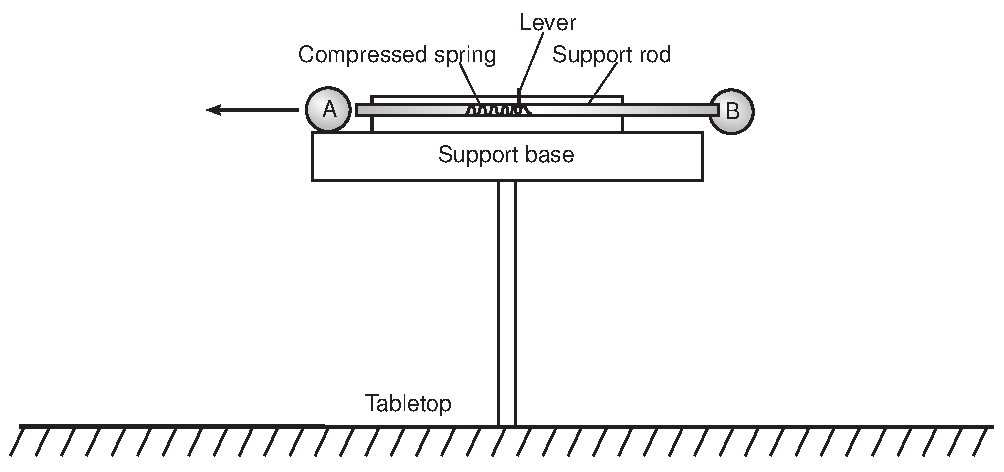
\includegraphics[keepaspectratio,width=0.95\linewidth]{June2012-Q45}
    \end{center}
    When the lever is released, the support rod withdraws from ball $A$, allowing it to fall.
    At the same instant, the rod contacts ball $A$, propelling it horizontally to the left.
    Which statement describes the motion that is observed after the lever is released and the balls fall?
    [Neglect friction.]
    \begin{choices}
        \wrongchoice{Ball $A$ travels at constant velocity.}
      \correctchoice{Ball $A$ hits the tabletop at the same times as ball $B$.}
        \wrongchoice{Ball $B$ hits the tabletop before ball $A$.}
        \wrongchoice{Ball $B$ travels with an increasing acceleration.}
    \end{choices}
\end{question}
}


%% Section June2011
%%--------------------
\element{nysed}{
\begin{question}{June2011-Q11}
    Four identical projectiles are launched with the same initial speed, $v$,
        but at various angles above the level ground.
    Which diagram represents the initial velocity of the projectile that will have the largest total horizontal displacement?
    [Neglect air resistance.]
    \begin{multicols}{2}
    \begin{choices}
        \AMCboxDimensions{down=-1.5em}
        \wrongchoice{
            \begin{tikzpicture}
                \draw[white] (-1.5em,-1.5em) rectangle (2,1.75);
                \draw[dashed] (0,0) -- (2,0) node[pos=0.5,anchor=north] {Level Ground};
                \draw[thick,->] (0,0) -- (30:2) node[pos=0.5,anchor=south east] {$v$};
                \draw[<->] (1,0) arc (0:30:1) node[pos=0.5,anchor=west] {\ang{30}};
            \end{tikzpicture}
        }
        \correctchoice{
            \begin{tikzpicture}
                \draw[white] (-1.5em,-1.5em) rectangle (2,2);
                \draw[dashed] (0,0) -- (2,0) node[pos=0.5,anchor=north] {Level Ground};
                \draw[thick,->] (0,0) -- (45:2) node[pos=0.5,anchor=south east] {$v$};
                \draw[<->] (1,0) arc (0:45:1) node[pos=0.5,anchor=west] {\ang{45}};
            \end{tikzpicture}
        }
        \wrongchoice{
            \begin{tikzpicture}
                \draw[white] (-1.5em,-1.5em) rectangle (2,2);
                \draw[dashed] (0,0) -- (2,0) node[pos=0.5,anchor=north] {Level Ground};
                \draw[thick,->] (0,0) -- (60:2) node[pos=0.5,anchor=south east] {$v$};
                \draw[<->] (1,0) arc (0:60:1) node[pos=0.5,anchor=west] {\ang{60}};
            \end{tikzpicture}
        }
        \wrongchoice{
            \begin{tikzpicture}
                \draw[white] (-1.5em,-1.5em) rectangle (2,2);
                \draw[dashed] (0,0) -- (2,0) node[pos=0.5,anchor=north] {Level Ground};
                \draw[thick,->] (0,0) -- (70:2) node[pos=0.5,anchor=south east] {$v$};
                \draw[<->] (1,0) arc (0:70:1) node[pos=0.5,anchor=west] {\ang{70}};
            \end{tikzpicture}
        }
    \end{choices}
    \end{multicols}
\end{question}
}


%% Section June2010
%%--------------------
\element{nysed}{
\begin{question}{June2010-Q06}
    As shown in the diagram below,
        a student standing on the roof of a \SI{50.0}{\meter} high building kicks a stone at a horizontal speed of \SI{4.00}{\meter\per\second}.
    \begin{center}
    \begin{tikzpicture}[yscale=0.75]
        \draw[very thick] (-2,0) -- (0,0) -- (0,-4) -- (3,-4);
        \draw[fill] (0.2,0.0) circle [radius=2pt];
        \draw[thick,->] (0.2,0.0) -- ++ (0:1)
            node[anchor=south] at ++ (0:-0.5) {$v=\SI{4.00}{\meter\per\second}$};
        \draw[very thick,dashed] (-2,-4) -- (0,-4);
        \node (A) at (-1,-2.0) {\SI{50}{\meter}};
        \draw[very thick,->] (A) -- (-1,0);
        \draw[very thick,->] (A) -- (-1,-4);
    \end{tikzpicture}
    \end{center}
    How much time is required for the stone to reach the level ground below?
    [Neglect friction.]
    \begin{multicols}{2}
    \begin{choices}
      \correctchoice{\SI{3.19}{\second}}
        \wrongchoice{\SI{5.10}{\second}}
        \wrongchoice{\SI{10.2}{\second}}
        \wrongchoice{\SI{12.5}{\second}}
    \end{choices}
    \end{multicols}
\end{question}
}

\element{nysed}{
\begin{question}{June2010-Q14}
    Four projectiles, $I$, $J$, $K$, and $L$,
        were launched from, and returned to, level ground.
    The data table below shows the initial horizontal speed,
        initial vertical speed, and time of flights for each projectile.
    Which projectile traveled the greatest horizontal distance?
    [Neglect friction.]
    \begin{center}
    \begin{tabu}{cX[c]X[c]X[c]}
        \toprule
        \makebox[1.5em][c]{\textnumero} &
        Initial Horizontal Speed [\si{\meter\per\second}] &
        Initial Vertical Speed [\si{\meter\per\second}] &
        Time of Flight [\si{\second}] \\
        \bottomrule
    \end{tabu}
    \end{center}
    \begin{choices}
        \wrongchoice{\begin{tabu}{X[c]X[c]X[c]} 40.0 & 29.4 & 6.00 \\ \end{tabu}}
        \wrongchoice{\begin{tabu}{X[c]X[c]X[c]} 60.0 & 19.6 & 4.00 \\ \end{tabu}}
        \wrongchoice{\begin{tabu}{X[c]X[c]X[c]} 50.0 & 24.5 & 5.00 \\ \end{tabu}}
      \correctchoice{\begin{tabu}{X[c]X[c]X[c]} 80.0 & 19.6 & 4.00 \\ \end{tabu}}
    \end{choices}
\end{question}
}


\element{nysed}{
\begin{question}{June2010-Q42}
    A student throws a baseball vertically upward and then catches it.
    If vertically upward is considered to be the positive direction,
        which graph best represents the relationship between velocity and time for the baseball?
    [Neglect friction.]
    \begin{multicols}{2}
    \begin{choices}
        \AMCboxDimensions{down=-1.5em}
        \correctchoice{
            \begin{tikzpicture}
                \begin{axis}[
                    axis y line=left,
                    axis x line=middle,
                    axis line style={->},
                    xlabel={time},
                    xtick=\empty,
                    ylabel={velocity},
                    ytick=\empty,
                    xmin=0,xmax=11,
                    ymin=-5,ymax=6,
                    width=0.95\columnwidth,
                    very thin,
                ]
                \addplot[line width=1pt,domain=0:10]{5-x};
                \end{axis}
            \end{tikzpicture}
        }
        \wrongchoice{
            \begin{tikzpicture}
                \begin{axis}[
                    axis y line=left,
                    axis x line=middle,
                    axis line style={->},
                    xlabel={time},
                    xtick=\empty,
                    x label style={anchor=north east},
                    ylabel={velocity},
                    ytick=\empty,
                    xmin=0,xmax=11,
                    ymin=-5,ymax=6,
                    width=0.95\columnwidth,
                    very thin,
                ]
                \addplot[line width=1pt,domain=0:5]{x};
                \addplot[line width=1pt,domain=5:10]{10-x};
                \end{axis}
            \end{tikzpicture}
        }
        \wrongchoice{
            \begin{tikzpicture}
                \begin{axis}[
                    axis y line=left,
                    axis x line=middle,
                    axis line style={->},
                    xlabel={time},
                    xtick=\empty,
                    x label style={anchor=north east},
                    ylabel={velocity},
                    ytick=\empty,
                    xmin=0,xmax=11,
                    ymin=-5,ymax=6,
                    width=0.95\columnwidth,
                    very thin,
                ]
                \addplot[line width=1pt,domain=0:10]{-0.20*x*(x-10)};
                \end{axis}
            \end{tikzpicture}
        }
        \wrongchoice{
            \begin{tikzpicture}
                \begin{axis}[
                    axis y line=left,
                    axis x line=middle,
                    axis line style={->},
                    xlabel={time},
                    xtick=\empty,
                    x label style={anchor=north east},
                    ylabel={velocity},
                    ytick=\empty,
                    xmin=0,xmax=11,
                    ymin=-5,ymax=6,
                    width=0.95\columnwidth,
                    very thin,
                ]
                \addplot[line width=1pt,domain=0:5]{5-x};
                \addplot[line width=1pt,domain=5:10]{-5+x};
                \end{axis}
            \end{tikzpicture}
        }
    \end{choices}
    \end{multicols}
\end{question}
}


%% Section June2009
%%--------------------
\element{nysed}{
\begin{question}{June2009-Q06}
    A golf ball is given an initial speed of \SI{20}{\meter\per\second} and returns to level ground.
    Which launch angle above level ground results in the ball traveling the greatest distance?
    [Neglect friction.]
    \begin{multicols}{4}
    \begin{choices}
        \wrongchoice{\ang{60}}
      \correctchoice{\ang{45}}
        \wrongchoice{\ang{30}}
        \wrongchoice{\ang{15}}
    \end{choices}
    \end{multicols}
\end{question}
}


%% Section Jan2009
%%--------------------
\element{nysed}{
\begin{question}{Jan2009-Q08}
    The diagram below represents the path of a stunt car that is driven off a cliff,
        neglecting friction.
    \begin{center}
    \begin{tikzpicture}[font=\small,scale=1.2]
        %% Surface
        \draw[thick] (-1,0) -- (0,0) -- (0,-2) -- (4,-2);
        %% Labels: 0 m 
        \node[anchor=north] at (0,-2) {\SI{0}{\meter}};
        \draw[fill] (1,-0.1) circle (1.5pt) node[anchor=south] {$A$};
        %% Labels: A at 10 m 
        \draw[dashed] (1,-2) -- (1,-0.1);
        \node[anchor=north] at (1,-2) {\SI{10}{\meter}};
        %% Labels: B at 20 m 
        \draw[fill] (2,-0.85) circle (1.5pt) node[anchor=south] {$B$};
        \draw[dashed] (2,-2) -- (2,-0.85);
        \node[anchor=north] at (2,-2) {\SI{20}{\meter}};
        %% Path
        \node[thick,draw,fill=white!80!black,anchor=south,circle,minimum size=1em] (Car) at (-0.5em,0) {};
        %\draw[->] (Car.east) -- ++ (0:0.75cm) node[pos=0.5,anchor=south] {$v$};
        \draw[thick,dashed] (0,0.5em) parabola bend (0,0.5em) (3,-2);
    \end{tikzpicture}
    \end{center}
    Compared to the horizontal component of the car's velocity at point $A$,
        the horizontal component of the car's velocity at point $B$ is:
    \begin{multicols}{3}
    \begin{choices}
        \wrongchoice{smaller}
        \wrongchoice{greater}
      \correctchoice{the same}
    \end{choices}
    \end{multicols}
\end{question}
}


%% Section June2008
%%--------------------
\element{nysed}{
\begin{question}{June2008-Q02}
    A projectile launched at an angle of \ang{45} above the horizontal travels through the air.
    Compared to the projectile's theoretical path with no air friction,
        the actual trajectory of the projectile with air friction is:
    \begin{choices}
      \correctchoice{lower and shorter}
        \wrongchoice{lower and longer}
        \wrongchoice{higher and shorter}
        \wrongchoice{higher and longer}
    \end{choices}
\end{question}
}

\element{nysed}{
\begin{question}{June2008-Q06}
    Two stones, $A$ and $B$, are thrown horizontally from the top of a cliff.
    Stone $A$ has an initial speed of \SI{15}{\meter\per\second} and stone $B$ has an initial speed of \SI{30}{\meter\per\second}.
    Compared to the time it takes stone $A$ to reach the ground,
        the time it takes stone $B$ to reach the ground is:
    \begin{choices}
      \correctchoice{the same}
        \wrongchoice{twice as great}
        \wrongchoice{half as great}
        \wrongchoice{four times as great}
    \end{choices}
\end{question}
}


%% Section Jan2008
%%--------------------
\element{nysed}{
\begin{question}{Jan2008-Q07}
    Two spheres, $A$ and $B$, are simultaneously projected horizontally from the top of a tower.
    Sphere $A$ has a horizontal speed of \SI{40}{\meter\per\second} and sphere $B$ has a horizontal speed of \SI{20}{\meter\per\second}.
    Which statement best describes the time required for the spheres to reach the ground and the horizontal distance they travel?
    [Neglect friction and assume the ground is level.]
    \begin{choices}
        \wrongchoice{Both spheres hit the ground at the same time and at the same distance from the base of the tower}
      \correctchoice{Both spheres hit the ground at the same time, but sphere $A$ lands twice as far as sphere $B$ from the base of the tower.}
        \wrongchoice{Both spheres hit the ground at the same time, but sphere $B$ lands twice as far as sphere $A$ from the base of the tower.}
        \wrongchoice{Sphere $A$ hits the ground before sphere $B$, and sphere $A$ lands twice as far as sphere $B$ from the base of the tower.}
    \end{choices}
\end{question}
}


%% Section June2007
%%--------------------


%% Section Jan2007
%%--------------------
\element{nysed}{
\begin{question}{Jan2007-Q05}
    A machine launches a tennis ball at an angle of \ang{25} above the horizontal at a speed of \SI{14}{\meter\per\second}.
    The ball returns to level ground.
    Which combination of changes \emph{must} produce an increase in time of flight of a second launch?
    \begin{choices}
      \correctchoice{increase the launch angle and increase the ball's initial speed}
        \wrongchoice{increase the launch angle and decrease the ball's initial speed}
        \wrongchoice{decrease the launch angle and increase the ball's initial speed}
        \wrongchoice{decrease the launch angle and decrease the ball's initial speed}
    \end{choices}
\end{question}
}

\element{nysed}{
\begin{question}{Jan2007-Q07}
    A plane flying horizontally above Earth's surface at \SI{100}{\meter\per\second} drops a crate.
    The crate strikes the ground \SI{30.0}{\second} later.
    What is the magnitude of the horizontal component of the crate's velocity just before it strikes the ground?
    [Neglect friction.]
    \begin{multicols}{2}
    \begin{choices}
      \correctchoice{\SI{100}{\meter\per\second}}
        \wrongchoice{\SI{0}{\meter\per\second}}
        \wrongchoice{\SI{294}{\meter\per\second}}
        \wrongchoice{\SI{394}{\meter\per\second}}
    \end{choices}
    \end{multicols}
\end{question}
}


%% Section June2006
%%--------------------
\element{nysed}{
\begin{question}{June2006-Q44}
    A volleyball hit into the air has an initial speed of \SI{10.}{\meter\per\second}.
    Which vector best represents the angle above the horizontal that the ball should be hit to remain in the air for the greatest amount of time?
    \begin{multicols}{2}
    \begin{choices}
        \AMCboxDimensions{down=-1.5em}
        \correctchoice{
            \begin{tikzpicture}
                \draw[white] (-0.5,-0.5) rectangle (2.1,2.1);
                \draw[thick,->] (0,0) -- (90:2cm);
                \draw[thick,dashed] (0,0) -- (0:2cm);
                \node[anchor=north] at (0:1cm) {Horizontal};
                \node[anchor=south west] at (0:0) {\ang{90}};
            \end{tikzpicture}
        }
        \wrongchoice{
            \begin{tikzpicture}
                \draw[white] (-0.5,-0.5) rectangle (2.1,2.1);
                \draw[thick,->] (0,0) -- (60:2cm);
                \draw[thick,dashed] (0,0) -- (0:2cm);
                \node[anchor=north] at (0:1cm) {Horizontal};
                \node[anchor=south east] at (0:1cm) {\ang{60}};
            \end{tikzpicture}
        }
        \wrongchoice{
            \begin{tikzpicture}
                \draw[white] (-0.5,-0.5) rectangle (2.1,2.1);
                \draw[thick,->] (0,0) -- (45:2cm);
                \draw[thick,dashed] (0,0) -- (0:2cm);
                \node[anchor=north] at (0:1cm) {Horizontal};
                \node[anchor=south] at (0:1cm) {\ang{45}};
            \end{tikzpicture}
        }
        \wrongchoice{
            \begin{tikzpicture}
                \draw[white] (-0.5,-0.5) rectangle (2.1,2.1);
                \draw[thick,->] (0,0) -- (30:2cm);
                \draw[thick,dashed] (0,0) -- (0:2cm);
                \node[anchor=north] at (0:1cm) {Horizontal};
                \node[anchor=south west] at (0:1cm) {\ang{30}};
            \end{tikzpicture}
        }
    \end{choices}
    \end{multicols}
\end{question}
}


%% Section Jan2006
%%--------------------


%% Section June2005
%%--------------------
\element{nysed}{
\begin{question}{June2005-Q05}
    A golf ball is hit at an angle of \ang{45} above the horizontal.
    What is the acceleration of the gold ball at the highest point in its trajectory?
    [Neglect friction.]
    \begin{choices}
      \correctchoice{\SI{9.8}{\meter\per\second\squared} downward}
        \wrongchoice{\SI{9.8}{\meter\per\second\squared} upward}
        \wrongchoice{\SI{6.9}{\meter\per\second\squared} horizontal}
        \wrongchoice{\SI{0.0}{\meter\per\second\squared}}
    \end{choices}
\end{question}
}

\element{nysed}{
\begin{question}{June2005-Q07}
    A ball is thrown horizontally at a speed of \SI{24}{\meter\per\second} from the top of a cliff.
    If the ball hits the ground \SI{4.0}{\second} later,
        approximately how high is the cliff?
    \begin{multicols}{2}
    \begin{choices}
      \correctchoice{\SI{78}{\meter}}
        \wrongchoice{\SI{96}{\meter}}
        \wrongchoice{\SI{6.0}{\meter}}
        \wrongchoice{\SI{39}{\meter}}
    \end{choices}
    \end{multicols}
\end{question}
}


%% Section Jan2005
%%--------------------


%% Section June2004
%%--------------------
\element{nysed}{
\begin{question}{June2004-Q04}
    The diagram below represents the path of an object after it was thrown.
    \begin{center}
    \begin{tikzpicture}
        \draw [very thick,domain=-2:2, samples=50] plot (\x, {2 - 0.20*\x*\x});
        \node [anchor=south] at (0,2) {$A$};
        \draw[fill] (0,2) circle (2pt);
        \node [anchor=south] at (1,1.80) {$B$};
        \draw[fill] (1,1.80) circle (2pt);
    \end{tikzpicture}
    \end{center}
    What happens to the object's acceleration as it travels from $A$ to $B$?
    [Neglect friction.]
    \begin{choices}
      \correctchoice{It remains the same}
        \wrongchoice{It increases}
        \wrongchoice{It decreases}
    \end{choices}
\end{question}
}

\element{nysed}{
\begin{question}{June2004-Q05}
    A \SI{0.2}{\kilo\gram} red ball is thrown horizontally at a speed of \SI{4}{\meter\per\second} from a height of \SI{3}{\meter}.
    A \SI{0.4}{\kilo\gram} green ball is thrown horizontally from the same height at a speed of \SI{8}{\meter\per\second}.
    Compared to the time it takes the red ball to reach the ground,
        the time it takes the green ball to reach the ground is:
    \begin{choices}
      \correctchoice{the same}
        \wrongchoice{one-half as great}
        \wrongchoice{twice as great}
        \wrongchoice{four times as great}
    \end{choices}
\end{question}
}


%% Section Jan2004
%%--------------------
\element{nysed}{
\begin{question}{Jan2004-Q06}
    A child kicks a ball with an initial velocity of \SI{8.5}{\meter\per\second} at an angle of \ang{35} with the horizontal,
        as shown.
    The ball has an initial velocity of \SI{4.9}{\meter\per\second} and a total time of flight of \SI{1.0}{\second}.
    [Neglect air resistance.]
    \begin{center}
        %% Part I of two part question
        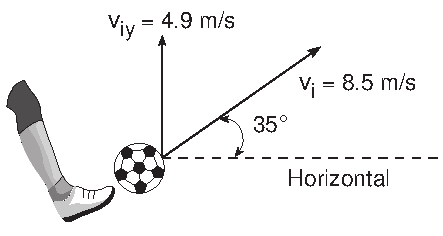
\includegraphics[keepaspectratio,width=0.80\linewidth]{Jan2004-Q06}
    \end{center}
    The horizontal component of the ball's initial velocity is approximately
    \begin{multicols}{2}
    \begin{choices}
      \correctchoice{\SI{7.0}{\meter\per\second}}
        \wrongchoice{\SI{13}{\meter\per\second}}
        \wrongchoice{\SI{3.6}{\meter\per\second}}
        \wrongchoice{\SI{4.9}{\meter\per\second}}
    \end{choices}
    \end{multicols}
\end{question}
}

\element{nysed}{
\begin{question}{Jan2004-Q07}
    A child kicks a ball with an initial velocity of \SI{8.5}{\meter\per\second} at an angle of \ang{35} with the horizontal,
        as shown.
    The ball has an initial velocity of \SI{4.9}{\meter\per\second} and a total time of flight of \SI{1.0}{\second}.
    [Neglect air resistance.]
    \begin{center}
        %% Part II of two part question
        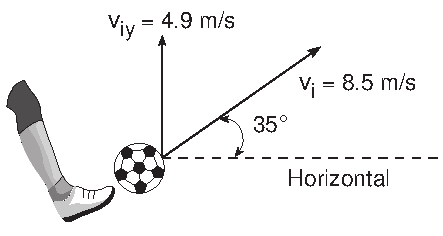
\includegraphics[keepaspectratio,width=0.80\linewidth]{Jan2004-Q06}
    \end{center}
    The maximum height reached by the ball is approximately:
    \begin{multicols}{2}
    \begin{choices}
      \correctchoice{\SI{1.2}{\meter}}
        \wrongchoice{\SI{2.5}{\meter}}
        \wrongchoice{\SI{4.9}{\meter}}
        \wrongchoice{\SI{8.5}{\meter}}
    \end{choices}
    \end{multicols}
\end{question}
}


%% Section June2003
%%--------------------
\element{nysed}{
\begin{question}{June2003-Q04}
    A ball is thrown at an angle of \ang{33} to the horizontal.
    What happens to the magnitude of the ball's vertical acceleration during the total time interval that the ball is in the air?
    \begin{choices}
        \wrongchoice{It decreases, then increases}
        \wrongchoice{It decreases, then remains the same}
        \wrongchoice{It increases, then decreases}
      \correctchoice{It remains the same}
    \end{choices}
\end{question}
}

\element{nysed}{
\begin{question}{June2003-Q06}
    Projectile A is launched horizontally at a speed of \SI{20}{\meter\per\second} from the top of a cliff and strikes a level surface below,
        \SI{3.0}{\second} later.
    Projectile B is launched horizontally from the same location at a speed of \SI{30}{\meter\per\second}.
    The time it takes projectile B to reach the level surface is:
    \begin{multicols}{2}
    \begin{choices}
      \correctchoice{\SI{3.0}{\second}}
        \wrongchoice{\SI{4.5}{\second}}
        \wrongchoice{\SI{2.0}{\second}}
        \wrongchoice{\SI{10}{\second}}
    \end{choices}
    \end{multicols}
\end{question}
}

\element{nysed}{
\begin{question}{June2003-Q07}
    Projectile A is launched horizontally at a speed of \SI{20}{\meter\per\second} from the top of a cliff and strikes a level surface below,
        \SI{3.0}{\second} later.
    Projectile B is launched horizontally from the same location at a speed of \SI{30}{\meter\per\second}.
    Approximately how high is the cliff?
    \begin{multicols}{2}
    \begin{choices}
      \correctchoice{\SI{44}{\meter}}
        \wrongchoice{\SI{29}{\meter}}
        \wrongchoice{\SI{60}{\meter}}
        \wrongchoice{\SI{104}{\meter}}
    \end{choices}
    \end{multicols}
\end{question}
}


%% Section Jan2003
%%--------------------


%% Section Aug2002
%%--------------------
\element{nysed}{
\begin{question}{Aug2002-Q38}
    An archer uses a bow to fire two similar arrows with the same string force.
    One arrow is fired at an angle of \ang{60} with the horizontal,
        and the other is fired at an angle of \ang{45} with the horizontal.
    Compared to the arrow fired at \ang{60},
        the arrow fired at \ang{45} has a:
    \begin{choices}
        \wrongchoice{longer flight time and longer horizontal range}
        \wrongchoice{longer flight time and shorter horizontal range}
      \correctchoice{shorter flight time and longer horizontal range}
        \wrongchoice{shorter flight time and shorter horizontal range}
    \end{choices}
\end{question}
}



%% Section June2002
%%--------------------
\element{nysed}{
\begin{question}{June2002-Q05}
    The diagram below shows a student throwing a baseball horizontally at \SI{25}{\meter\per\second} from a cliff \SI{45}{\meter} above the level ground.
    \begin{center}
    \begin{tikzpicture}[yscale=0.75]
        \draw[very thick] (-2,0) -- (0,0) -- (0,-4) -- (3,-4);
        \draw[fill] (0.2,0.0) circle [radius=2pt];
        \draw[thick,->] (0.2,0.0) -- ++ (0:1)
            node[anchor=south] at ++ (0:-0.5) {$v=\SI{25}{\meter\per\second}$};
        \draw[very thick,dashed] (-2,-4) -- (0,-4);
        \node (A) at (-1,-2.0) {\SI{45}{\meter}};
        \draw[very thick,->] (A) -- (-1,0);
        \draw[very thick,->] (A) -- (-1,-4);
    \end{tikzpicture}
    \end{center}
    Approximately how far from the base of the cliff does the ball hit the ground?
    [Neglect air resistance]
    \begin{multicols}{2}
    \begin{choices}
        \wrongchoice{\SI{45}{\meter}}
      \correctchoice{\SI{75}{\meter}}
        \wrongchoice{\SI{140}{\meter}}
        \wrongchoice{\SI{230}{\meter}}
    \end{choices}
    \end{multicols}
\end{question}
}

\element{nysed}{
\begin{question}{June2002-Q06}
    A projectile is fired from a gun near the surface of Earth.
    The initial velocity of the projectile has a vertical component of \SI{98}{\meter\per\second} and a horizontal component of \SI{49}{\meter\per\second}.
    How long will it take the projectile to reach the highest point in its path?
    \begin{multicols}{2}
    \begin{choices}
        \wrongchoice{\SI{5.0}{\second}}
        \wrongchoice{\SI{10}{\second}}
        \wrongchoice{\SI{20}{\second}}
      \correctchoice{\SI{100}{\second}}
    \end{choices}
    \end{multicols}
\end{question}
}


%% Section Jan2002
%%--------------------
\element{nysed}{
\begin{question}{Jan2002-Q06}
    Which two terms represent a vector quantity and the scalar quantity of the vector's magnitude respectively?
    \begin{choices}
        \wrongchoice{acceleration and velocity}
        \wrongchoice{weight and force}
        \wrongchoice{speed and time}
      \correctchoice{displacement and distance}
    \end{choices}
\end{question}
}
 
\element{nysed}{
\begin{question}{Jan2002-Q07}
    A \SI{4.0}{\kilo\gram} rock and a \SI{1.0}{\kilo\gram} stone fall freely from rest from a height of \SI{100}{\meter}.
    After they fall for \SI{2.0}{\second},
        the ratio of the rock's speed to the stone's speed is:
    \begin{multicols}{2}
    \begin{choices}
      \correctchoice{$1:1$}
        \wrongchoice{$1:2$}
        \wrongchoice{$2:1$}
        \wrongchoice{$4:1$}
    \end{choices}
    \end{multicols}
\end{question}
}

\element{nysed}{
\begin{question}{Jan2002-Q56}
    A ball is thrown horizontally with an initial velocity of \SI{20.0}{\meter\per\second} from the top of a tower \SI{60.0}{\meter} high.
    \begin{center}
        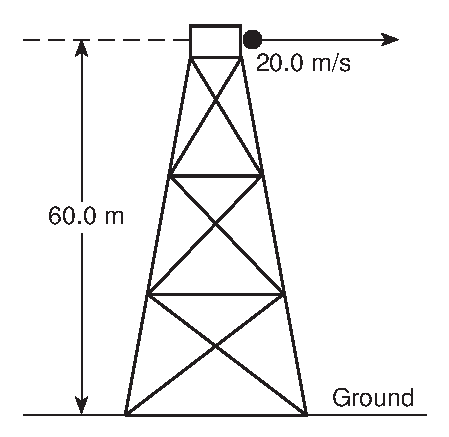
\includegraphics[keepaspectratio,scale=0.95]{Jan2002-Q56}
    \end{center}
    What is the initial vertical velocity of the ball?
    \begin{multicols}{2}
    \begin{choices}
      \correctchoice{\SI{0}{\meter\per\second}}
        \wrongchoice{\SI{9.81}{\meter\per\second}}
        \wrongchoice{\SI{20.0}{\meter\per\second}}
        \wrongchoice{\SI{60.0}{\meter\per\second}}
    \end{choices}
    \end{multicols}
\end{question}
}

\element{nysed}{
\begin{question}{Jan2002-Q57}
    A ball is thrown horizontally with an initial velocity of \SI{20.0}{\meter\per\second} from the top of a tower \SI{60.0}{\meter} high.
    \begin{center}
        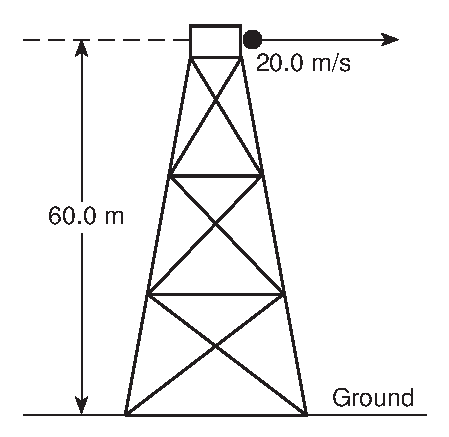
\includegraphics[keepaspectratio,scale=0.95]{Jan2002-Q56}
    \end{center}
    What is the approximate total time required for the ball to reach the ground?
    [Neglect air resistance]
    \begin{multicols}{2}
    \begin{choices}
        \wrongchoice{\SI{12.2}{\second}}
        \wrongchoice{\SI{2.04}{\second}}
        \wrongchoice{\SI{3.00}{\second}}
      \correctchoice{\SI{3.50}{\second}}
    \end{choices}
    \end{multicols}
\end{question}
}

\element{nysed}{
\begin{question}{Jan2002-Q58}
    A ball is thrown horizontally with an initial velocity of \SI{20.0}{\meter\per\second} from the top of a tower \SI{60.0}{\meter} high.
    \begin{center}
        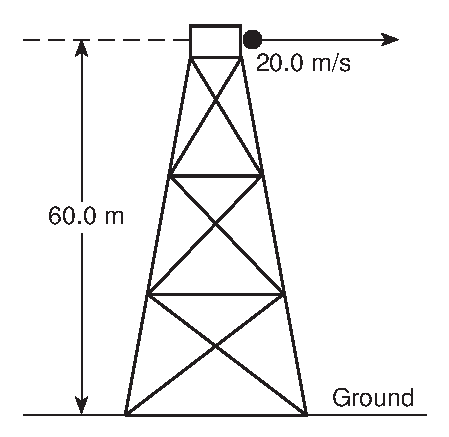
\includegraphics[keepaspectratio,scale=0.95]{Jan2002-Q56}
    \end{center}
    What is the horizontal velocity of the ball just before it reaches the ground?
    [Neglect air resistance.]
    \begin{multicols}{2}
    \begin{choices}
        \wrongchoice{\SI{9.81}{\meter\per\second}}
      \correctchoice{\SI{20.0}{\meter\per\second}}
        \wrongchoice{\SI{34.3}{\meter\per\second}}
        \wrongchoice{\SI{68.6}{\meter\per\second}}
    \end{choices}
    \end{multicols}
\end{question}
}

\element{nysed}{
\begin{question}{Jan2002-Q62}
    A golf ball leaves a golf club with an initial velocity of \SI{40}{\meter\per\second} at an angle of \ang{40} with respect to the horizontal.
    \begin{center}
        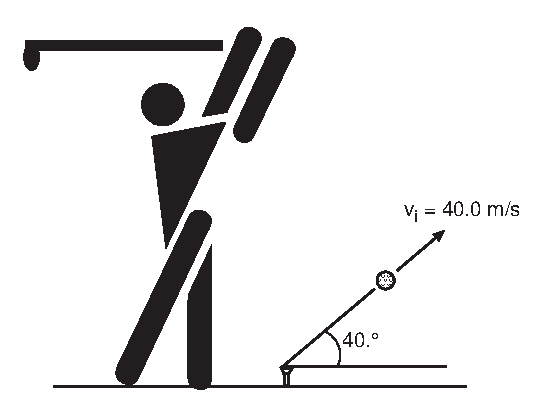
\includegraphics[keepaspectratio,scale=0.90]{Jan2002-Q62}
    \end{center}
    What is the vertical component of the golf ball's initial velocity?
    \begin{multicols}{2}
    \begin{choices}
      \correctchoice{\SI{25.7}{\meter\per\second}}
        \wrongchoice{\SI{30.6}{\meter\per\second}}
        \wrongchoice{\SI{40.0}{\meter\per\second}}
        \wrongchoice{\SI{61.3}{\meter\per\second}}
    \end{choices}
    \end{multicols}
\end{question}
}

\element{nysed}{
\begin{question}{Jan2002-Q63}
    A golf ball leaves a golf club with an initial velocity of \SI{40}{\meter\per\second} at an angle of \ang{40} with respect to the horizontal.
    \begin{center}
        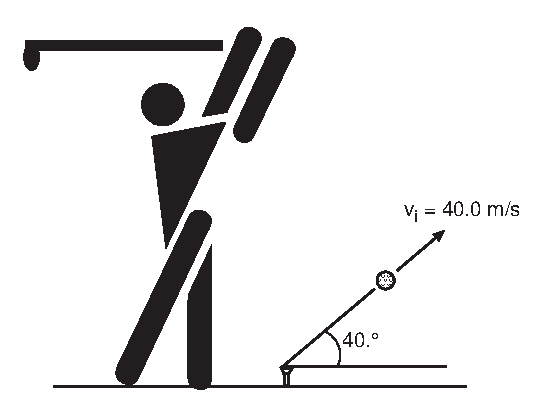
\includegraphics[keepaspectratio,scale=0.90]{Jan2002-Q62}
    \end{center}
    What is the total horizontal distance traveled by the golf ball during the first \SI{2.5}{\second} of its flight?
    \begin{multicols}{2}
    \begin{choices}
        \wrongchoice{\SI{100}{\meter}}
      \correctchoice{\SI{76.6}{\meter}}
        \wrongchoice{\SI{64.3}{\meter}}
        \wrongchoice{\SI{40.0}{\meter}}
    \end{choices}
    \end{multicols}
\end{question}
}


%% Section June2001
%%--------------------
\element{nysed}{
\begin{question}{June2001-Q58}
    A red ball and a green ball are simultaneously thrown horizontally from the same height.
    The red ball has an initial speed of \SI{40}{\meter\per\second} and the green ball has an initial speed of \SI{20}{\meter\per\second}.
    Compared to the time it takes the red ball to reach the ground,
        the time it takes the green ball to reach the ground will be:
    \begin{choices}
      \correctchoice{the same}
        \wrongchoice{half as much}
        \wrongchoice{twice as much}
        \wrongchoice{four times as much}
    \end{choices}
\end{question}
}

\element{nysed}{
\begin{question}{June2001-Q59}
    A baseball player throws a ball horizontally.
    Which statement best describes the ball's motion after it is thrown?
    [Neglect the effect of friction.]
    \begin{choices}
        \wrongchoice{Its vertical speed remains the same, and its horizontal speed increases.}
        \wrongchoice{Its vertical speed remains the same, and its horizontal speed remains the same.}
        \wrongchoice{Its vertical speed increases, and its horizontal speed increases.}
      \correctchoice{Its vertical speed increases, and its horizontal speed remains the same.}
    \end{choices}
\end{question}
}


%% Section Jan2001
%%--------------------
\element{nysed}{
\begin{question}{Jan2001-Q58}
    A red ball and a green ball are simultaneously thrown horizontally from the same height.
    the red ball has an initial speed of \SI{40}{\meter\per\second} and the green ball has an initial speed of \SI{20}{\meter\per\second}.
    Compared to the the time it takes the red ball to reach the ground,
        the time it takes the green ball to reach the ground will be:
    \begin{choices}
      \correctchoice{the same}
        \wrongchoice{twice as much}
        \wrongchoice{half as much}
        \wrongchoice{four times as much}
    \end{choices}
\end{question}
}

\element{nysed}{
\begin{question}{Jan2001-Q62}
    The path of a projectile fired at a \ang{30} to the horizontal is best described as:
    \begin{multicols}{2}
    \begin{choices}
      \correctchoice{parabolic}
        \wrongchoice{linear}
        \wrongchoice{circular}
        \wrongchoice{hyperbolic}
    \end{choices}
    \end{multicols}
\end{question}
}


%% Section June2000
%%--------------------
\element{nysed}{
\begin{question}{June2000-Q56}
    A machine launches a tennis ball at an angle of \ang{45} with the horizontal,
        as shown.
    The ball has an initial vertical velocity of \SI{9.0}{\meter\per\second} and an initial horizontal velocity of \SI{9.0}{\meter\per\second}.
    The ball reaches its maximum height \SI{0.92}{\second} after its launch.
    [Neglect air resistance and assume the ball lands at the same height above the ground from which it was launched.]
    \begin{center}
        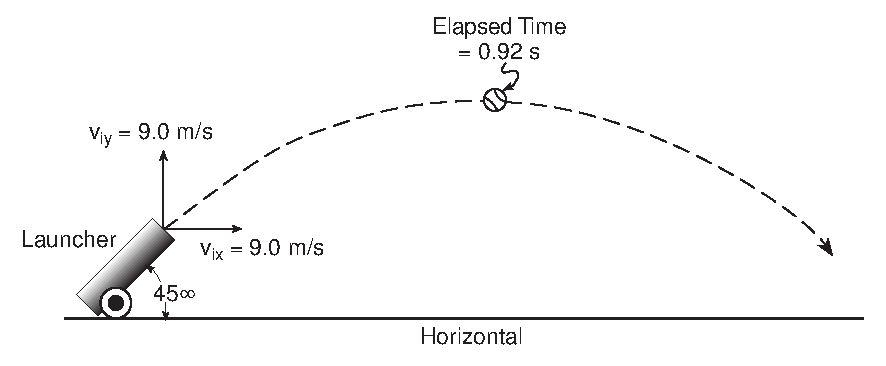
\includegraphics[keepaspectratio,width=\columnwidth]{June2000-Q56}
    \end{center}
    The speed of the tennis ball as it leaves the launcher is approximately:
    \begin{multicols}{2}
    \begin{choices}
        \wrongchoice{\SI{4.5}{\meter\per\second}}
      \correctchoice{\SI{13}{\meter\per\second}}
        \wrongchoice{\SI{8.3}{\meter\per\second}}
        \wrongchoice{\SI{18}{\meter\per\second}}
    \end{choices}
    \end{multicols}
\end{question}
}

\element{nysed}{
\begin{question}{June2000-Q57}
    A machine launches a tennis ball at an angle of \ang{45} with the horizontal,
        as shown.
    The ball has an initial vertical velocity of \SI{9.0}{\meter\per\second} and an initial horizontal velocity of \SI{9.0}{\meter\per\second}.
    The ball reaches its maximum height \SI{0.92}{\second} after its launch.
    [Neglect air resistance and assume the ball lands at the same height above the ground from which it was launched.]
    \begin{center}
        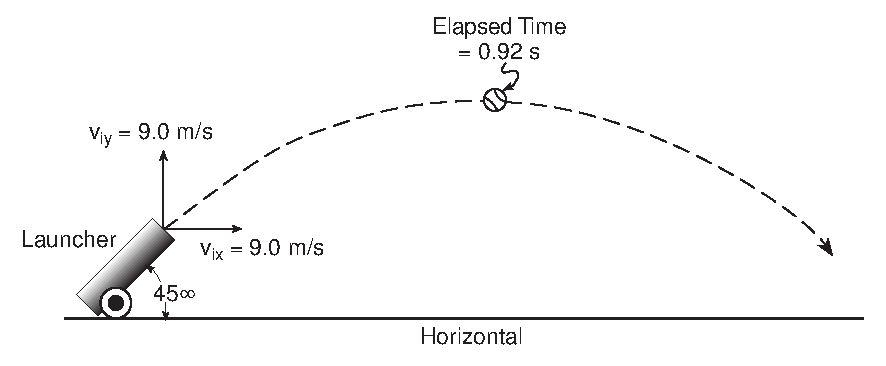
\includegraphics[keepaspectratio,width=\columnwidth]{June2000-Q56}
    \end{center}
    The total horizontal distance traveled by the tennis ball during the entire time it is in the air is approximately:
    \begin{multicols}{2}
    \begin{choices}
        \wrongchoice{\SI{23}{\meter}}
        \wrongchoice{\SI{17}{\meter}}
      \correctchoice{\SI{8.3}{\meter}}
        \wrongchoice{\SI{4.1}{\meter}}
    \end{choices}
    \end{multicols}
\end{question}
}

\element{nysed}{
\begin{question}{June2000-Q58}
    A machine launches a tennis ball at an angle of \ang{45} with the horizontal,
        as shown.
    The ball has an initial vertical velocity of \SI{9.0}{\meter\per\second} and an initial horizontal velocity of \SI{9.0}{\meter\per\second}.
    The ball reaches its maximum height \SI{0.92}{\second} after its launch.
    [Neglect air resistance and assume the ball lands at the same height above the ground from which it was launched.]
    \begin{center}
        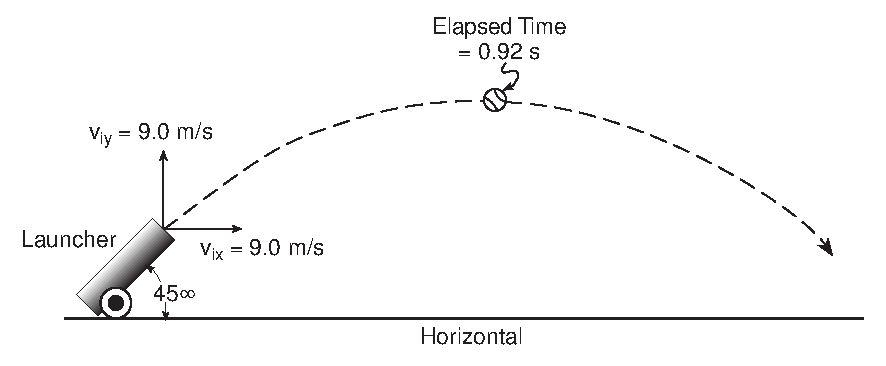
\includegraphics[keepaspectratio,width=\columnwidth]{June2000-Q56}
    \end{center}
    The speed at which the launcher fires tennis balls is constant,
        but the angle between the launcher and the horizontal can be varied.
    As the angle is decreased from \ang{45} to \ang{30},
        the range of the tennis balls:
    \begin{choices}
      \correctchoice{decreases}
        \wrongchoice{increases}
        \wrongchoice{remains the same}
    \end{choices}
\end{question}
}

\element{nysed}{
\begin{question}{June2000-Q59}
    A \SI{2}{\kilo\gram} block is dropped from the roof of a tall building at the same time a \SI{6}{\kilo\gram} ball is thrown horizontally from the same height.
    Which statement best describes the motion of the block and the motion of the ball? [Neglect air resistance]
    \begin{choices}
        \wrongchoice{The \SI{2}{\kilo\gram} block hits the ground first because it has no horizontal velocity.}
        \wrongchoice{The \SI{6}{\kilo\gram} block hits the ground first because it has more mass.}
        \wrongchoice{The \SI{6}{\kilo\gram} block hits the ground first because it is round.}
      \correctchoice{The block and the ball hit the ground at the same time because they have the same vertical acceleration}
    \end{choices}
\end{question}
}


%% Section June1999
%%--------------------
\element{nysed}{
\begin{question}{June1999-Q58}
    The diagram below shows the muzzle of a cannon located \SI{50}{\meter} above the ground.
    When the cannon is fired, a ball leaves the muzzle with an initial speed of \SI{250}{\meter\per\second}.
    [Neglect air resistance]
    \begin{center}
    \begin{tikzpicture}[yscale=0.75]
        \draw[very thick] (-2,0) -- (0,0) -- (0,-4) -- (3,-4);
        \draw[fill] (0.2,0.0) circle [radius=2pt];
        \draw[thick,->] (0.2,0.0) -- ++ (0:1)
            node[anchor=south] at ++ (0:-0.5) {$v=\SI{250}{\meter\per\second}$};
        \draw[very thick,dashed] (-2,-4) -- (0,-4);
        \node (A) at (-1,-2.0) {\SI{50}{\meter}};
        \draw[very thick,->] (A) -- (-1,0);
        \draw[very thick,->] (A) -- (-1,-4);
    \end{tikzpicture}
    \end{center}
    Which action would most likely increase the time of flight of the ball fired by the cannon?
    \begin{choices}
        \wrongchoice{pointing the muzzle of the cannon toward the ground}
        \wrongchoice{moving the cannon closer to the edge of the cliff}
      \correctchoice{positioning the cannon higher above the ground}
        \wrongchoice{giving the ball a greater initial horizontal velocity}
    \end{choices}
\end{question}
}

\element{nysed}{
\begin{question}{June1999-Q62}
    In the diagram below,
        a stationary observer on the ground watches as a seagull flying horizontally to the right drops a clamshell.
    \begin{center}
        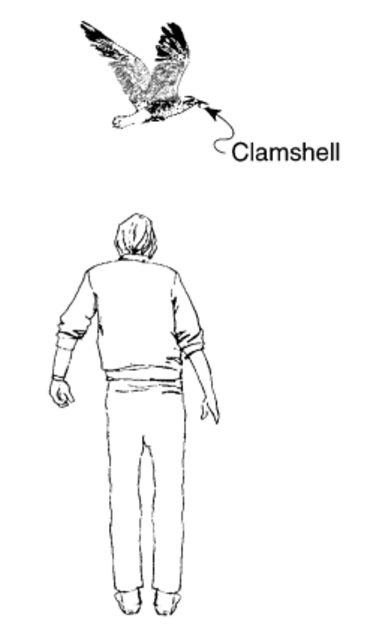
\includegraphics[keepaspectratio,scale=0.66]{June1999-Q62}
    \end{center}
    Which diagram best represents the path of the falling clamshell as seen by the observer?
    [Neglect air resistance]
    \begin{multicols}{2}
    \begin{choices}
        \AMCboxDimensions{down=-0.40cm}
        \wrongchoice{
            \begin{tikzpicture}
                \draw[white] (-0.5,0) rectangle (0.5,-1);
                \draw[thick,->] (0,0) -- (0,-1);
            \end{tikzpicture}
        }
        \wrongchoice{
            \begin{tikzpicture}
                \draw[white] (-0.15,+0.15) rectangle (+0.85,-0.85);
                \draw[thick,->] (0,0) -- (0.707,-0.707);
            \end{tikzpicture}
        }
        \wrongchoice{
            \begin{tikzpicture}
                \draw[white] (-0.25,0) rectangle (0.75,-1);
                \draw[thick,->] (0,0) arc (90:-90:0.50);
            \end{tikzpicture}
        }
        \correctchoice{
            \begin{tikzpicture}
                \draw[white] (0,1) rectangle (1,0);
                \draw[thick,->] (0,1) parabola (1,0);
            \end{tikzpicture}
        }
    \end{choices}
    \end{multicols}
\end{question}
}


%% Section June1998
%%--------------------
\element{nysed}{
\begin{question}{June1998-Q56}
    A student standing on a knoll throws a snowball horizontally \SI{4.5}{\meter} above the level ground towards a smokestack \SI{15}{\meter} away.
    The snowball hits the smokestack \SI{0.65}{\second} after being released. 
    [Neglect air resistance]
    \begin{center}
        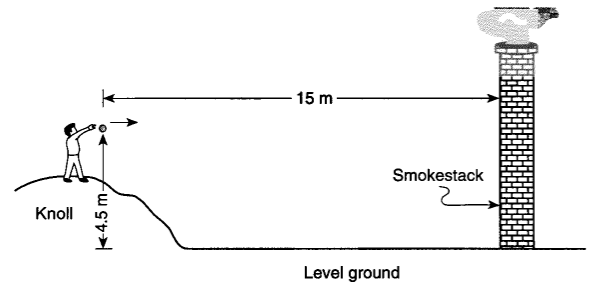
\includegraphics[keepaspectratio,width=\linewidth]{June1998-Q56}
    \end{center}
    Approximately how far above the level ground does the snowball hit the smokestack?
    \begin{multicols}{2}
    \begin{choices}
        \wrongchoice{\SI{0.0}{\meter}}
        \wrongchoice{\SI{0.4}{\meter}}
      \correctchoice{\SI{2.4}{\meter}}
        \wrongchoice{\SI{4.5}{\meter}}
    \end{choices}
    \end{multicols}
\end{question}
}

\element{nysed}{
\begin{question}{June1998-Q57}
    A student standing on a knoll throws a snowball horizontally \SI{4.5}{\meter} above the level ground towards a smokestack \SI{15}{\meter} away.
    The snowball hits the smokestack \SI{0.65}{\second} after being released. 
    [Neglect air resistance]
    \begin{center}
        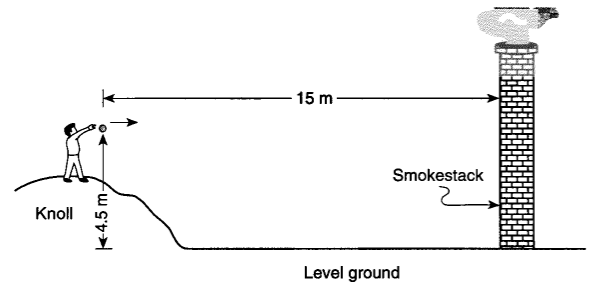
\includegraphics[keepaspectratio,width=0.95\linewidth]{June1998-Q56}
    \end{center}
    At the instant the snowball is released,
        the horizontal component of its velocity is approximately:
    \begin{multicols}{2}
    \begin{choices}
        \wrongchoice{\SI{6.9}{\meter\per\second}}
        \wrongchoice{\SI{9.8}{\meter\per\second}}
        \wrongchoice{\SI{17}{\meter\per\second}}
      \correctchoice{\SI{23}{\meter\per\second}}
    \end{choices}
    \end{multicols}
\end{question}
}

\element{nysed}{
\begin{question}{June1998-Q62}
    The diagram below shows a projectile moving with speed $v$ at the top of its trajectory.
    \begin{center}
    \begin{tikzpicture}
        %% Ground
        \draw[thick] (-3.5,0) -- (3.5,0);
        \node[anchor=north,fill,pattern=north east lines,minimum width=7cm, minimum height=0.05cm] at (0,0) {};
        \node[anchor=north] at (0,-1em) {Ground};
        %% Path: y = 2/9 x^2, y' = 4/9 x, dy/dx (2) = 12/9, atan(12/9) = 53
        \draw[thick,dashed] (-3,0) parabola bend (0,2) (3,0);
        \draw[thick,->] (-3,0) -- ++(53:1);
        %% Projectile
        \draw[fill] (0,2) circle (3pt) node[anchor=north,yshift=-3pt,font=\small] {Projectile};
        \draw[thick,->] (-0.5,2.4) -- (0.5,2.4) node[pos=0.5,anchor=south] {$v$};
    \end{tikzpicture}
    \end{center}
    Which vector best represents the acceleration of the projectile in the position shown?
    \begin{multicols}{4}
    \begin{choices}
        \AMCboxDimensions{down=-0.2cm}
        \correctchoice{
            \begin{tikzpicture}[scale=0.4]
                \draw[dashed,white!90!black] (0,0) rectangle (2,2);
                \draw[very thick,->] (1,2) -- (1,0);
            \end{tikzpicture}
        }
        \wrongchoice{
            \begin{tikzpicture}[scale=0.4]
                \draw[dashed,white!90!black] (0,0) rectangle (2,2);
                \draw[very thick,->] (2,1) -- (0,1);
            \end{tikzpicture}
        }
        \wrongchoice{
            \begin{tikzpicture}[scale=0.4]
                \draw[dashed,white!90!black] (0,0) rectangle (2,2);
                \draw[very thick,->] (1,0) -- (1,2);
            \end{tikzpicture}
        }
        \wrongchoice{
            \begin{tikzpicture}[scale=0.4]
                \draw[dashed,white!90!black] (0,0) rectangle (2,2);
                \draw[very thick,->] (1,2) -- (1,0);
            \end{tikzpicture}
        }
    \end{choices}
    \end{multicols}
\end{question}
}


%% Section June1997
%%--------------------
\element{nysed}{
\begin{question}{June1997-Q62}
    Projectiles are fired from different angles with the same speed of \SI{14}{\meter\per\second}.
    The graph below shows the range of the projectiles as a function of the original angle of inclination to the ground, neglecting air resistance.
    \begin{center}
    \begin{tikzpicture}
        \begin{axis}[
            axis y line=left, 
            axis x line=bottom, 
            axis line style={->},
            xlabel={Angle},
            x unit=\si{\degree},
            xtick={0,10,20,30,40,50,60,70,80,90},
            ylabel={Range},
            y unit=\si{\meter},
            ytick={0,5,10,15,20},
            grid=major,
            xmin=0,xmax=90,
            ymin=0,ymax=21,
            width=0.8\columnwidth,
            height=0.5\columnwidth,
        ]
        \addplot[line width=1pt,domain=0:90]{20*sin(2*x)};
        \end{axis}
    \end{tikzpicture}
    \end{center}
    The graph shows that the range of the projectile is:
    \begin{choices}
        \wrongchoice{the same for all angles.}
        \wrongchoice{the same for angles of \ang{20} and \ang{80}.}
      \correctchoice{greatest for an angle of \ang{45}.}
        \wrongchoice{greatest for an angle of \ang{90}.}
    \end{choices}
\end{question}
}

\element{nysed}{
\begin{question}{June1997-Q64}
    Four different balls are thrown horizontally off the top of four cliffs.
    In which diagram does the ball have the shortest time of flight?
    \begin{multicols}{2}
    \begin{choices}
        \AMCboxDimensions{down=-1cm}
        \correctchoice{
            \begin{tikzpicture}[font=\footnotesize]
                \draw[dashed,white!90!black] (-1.5,-1.2em) rectangle (1.5,4.3);
                %% Cliff
                \draw[thick] (-1,1) -- (0,1) -- (0,0) -- (1,0);
                \node[anchor=south,rotate=270] at (0,0.5) {Cliff};
                \node[anchor=north,rotate=0.0] at (0.5,0) {Ground};
                %% Height
                \draw[<->] (-0.9,1) -- (-0.9,0) node[pos=0.5,anchor=center,fill=white] {\SI{125}{\meter}};
                %% Mass
                \draw[fill] (0,1.33) circle (1.5pt) node[anchor=east] {\SI{1.0}{\kilo\gram}};
                %% velocity
                \draw[thick,->] (0,1.33) -- ++ (0:1) node[pos=0.5,anchor=south] {\SI{50}{\meter\per\second}};
            \end{tikzpicture}
        }
        \wrongchoice{
            \begin{tikzpicture}[font=\footnotesize]
                \draw[dashed,white!90!black] (-1.5,-1.2em) rectangle (1.5,4.3);
                %% Cliff
                \draw[thick] (-1,2) -- (0,2) -- (0,0) -- (1,0);
                \node[anchor=south,rotate=270] at (0,1.0) {Cliff};
                \node[anchor=north,rotate=0.0] at (0.5,0) {Ground};
                %% Height
                \draw[<->] (-0.9,2) -- (-0.9,0) node[pos=0.5,anchor=center,fill=white] {\SI{250}{\meter}};
                %% Mass
                \draw[fill] (0,2.33) circle (1.5pt) node[anchor=east] {\SI{0.5}{\kilo\gram}};
                %% velocity
                \draw[thick,->] (0,2.33) -- ++ (0:1) node[pos=0.5,anchor=south] {\SI{40}{\meter\per\second}};
            \end{tikzpicture}
        }
        \wrongchoice{
            \begin{tikzpicture}[font=\footnotesize]
                \draw[dashed,white!90!black] (-1.5,-1.2em) rectangle (1.5,4.3);
                %% Cliff
                \draw[thick] (-1,3) -- (0,3) -- (0,0) -- (1,0);
                \node[anchor=south,rotate=270] at (0,1.5) {Cliff};
                \node[anchor=north,rotate=0.0] at (0.5,0) {Ground};
                %% Height
                \draw[<->] (-0.9,3) -- (-0.9,0) node[pos=0.5,anchor=center,fill=white] {\SI{375}{\meter}};
                %% Mass
                \draw[fill] (0,3.33) circle (1.5pt) node[anchor=east] {\SI{0.25}{\kilo\gram}};
                %% velocity
                \draw[thick,->] (0,3.33) -- ++ (0:1) node[pos=0.5,anchor=south] {\SI{35}{\meter\per\second}};
            \end{tikzpicture}
        }
        \wrongchoice{
            \begin{tikzpicture}[font=\footnotesize]
                \draw[dashed,white!90!black] (-1.5,-1.2em) rectangle (1.5,4.3);
                %% Cliff
                \draw[thick] (-1,3.6) -- (0,3.6) -- (0,0) -- (1,0);
                \node[anchor=south,rotate=270] at (0,1.5) {Cliff};
                \node[anchor=north,rotate=0.0] at (0.5,0) {Ground};
                %% Height
                \draw[<->] (-0.9,3.6) -- (-0.9,0) node[pos=0.5,anchor=center,fill=white] {\SI{450}{\meter}};
                %% Mass
                \draw[fill] (0,3.9) circle (1.5pt) node[anchor=east] {\SI{0.1}{\kilo\gram}};
                %% velocity
                \draw[thick,->] (0,3.9) -- ++ (0:1) node[pos=0.5,anchor=south] {\SI{35}{\meter\per\second}};
            \end{tikzpicture}
        }
    \end{choices}
    \end{multicols}
\end{question}
}


%% Section June1996
%%--------------------
\newcommand{\JuneNineteenNinetySixQFiftySix}{
\begin{tikzpicture}
    %% NOTE: useful reference
    %% \frac{h}{R} = \frac{\tan\theta}{4}
    \draw[thick] (-3.5,0) -- (3.5,0);
    \draw[thick,dashed] (-3,0) parabola bend (0,1.05) (3,0);
    \draw[very thick,->] (-3,0) -- ++ (35:2.0cm) node[pos=1.0,anchor=south] {$v_i$};
    \draw[thick,<->] (-2,0) arc (0:35:1cm) node[pos=0.5,anchor=west] {\ang{35}};
\end{tikzpicture}
}

\element{nysed}{
\begin{question}{June1996-Q56}
    A cannon elevated at an angle of \ang{35} to the horizontal fires a cannonball,
        which travels the path shown in the diagram below.
    [Neglect air resistance and assume the ball lands at the same height above the ground from which it was launched.]
    \begin{center}
        \JuneNineteenNinetySixQFiftySix
    \end{center}
    If the ball lands \SI{7.0e2}{\meter} from the cannon \SI{10}{\second} after it was fired,
        what is the horizontal component of its initial velocity?
    \begin{multicols}{2}
    \begin{choices}
      \correctchoice{\SI{70}{\meter\per\second}}
        \wrongchoice{\SI{49}{\meter\per\second}}
        \wrongchoice{\SI{35}{\meter\per\second}}
        \wrongchoice{\SI{7.0}{\meter\per\second}}
    \end{choices}
    \end{multicols}
\end{question}
}

\element{nysed}{
\begin{question}{June1996-Q57}
    A cannon elevated at an angle of \ang{35} to the horizontal fires a cannonball,
        which travels the path shown in the diagram below.
    [Neglect air resistance and assume the ball lands at the same height above the ground from which it was launched.]
    \begin{center}
        \JuneNineteenNinetySixQFiftySix
    \end{center}
    If the ball's time of flight is \SI{10}{\second},
        what is the vertical component of its initial velocity?
    \begin{multicols}{2}
    \begin{choices}
        \wrongchoice{\SI{9.8}{\meter\per\second}}
      \correctchoice{\SI{49}{\meter\per\second}}
        \wrongchoice{\SI{70}{\meter\per\second}}
        \wrongchoice{\SI{98}{\meter\per\second}}
    \end{choices}
    \end{multicols}
\end{question}
}

\element{nysed}{
\begin{question}{June1996-Q58}
    A cannon elevated at an angle of \ang{35} to the horizontal fires a cannonball,
        which travels the path shown in the diagram below.
    [Neglect air resistance and assume the ball lands at the same height above the ground from which it was launched.]
    \begin{center}
        \JuneNineteenNinetySixQFiftySix
    \end{center}
    If the angle of elevation of the cannon is decreased from \ang{35} to \ang{30},
        the vertical component of the ball's initial velocity will:
    \begin{choices}
        \wrongchoice{decrease and its horizontal will decrease.}
      \correctchoice{decrease and its horizontal will increase.}
        \wrongchoice{increase and its horizontal will decrease.}
        \wrongchoice{increase and its horizontal will increase.}
    \end{choices}
\end{question}
}

\element{nysed}{
\begin{question}{June1996-Q65}
    A ball is projected horizontally to the right from a height of \SI{50}{\meter},
        as shown in the diagram below.
    \begin{center}
    \begin{tikzpicture}[yscale=0.75]
        \draw[very thick] (-2,0) -- (0,0) -- (0,-4) -- (3,-4);
        \draw[fill] (0.2,0.0) circle [radius=2pt];
        \draw[thick,->] (0.2,0.0) -- ++ (0:1)
            node[anchor=south] at ++ (0:-0.5) {$v$};
        \draw[very thick,dashed] (-2,-4) -- (0,-4);
        \node (A) at (-1,-2.0) {\SI{50}{\meter}};
        \draw[very thick,->] (A) -- (-1,0);
        \draw[very thick,->] (A) -- (-1,-4);
    \end{tikzpicture}
    \end{center}
    Which diagram best represents the position of the ball at \SI{1.0}{\second} intervals?
    [Neglect air resistance.]
    \begin{multicols}{2}
    \begin{choices}
        \AMCboxDimensions{down=-1.5em}
        \correctchoice{
            \begin{tikzpicture}[yscale=0.75]
                \draw[very thick] (0,0) -- (0,-4) -- (2,-4);
                \draw[domain=0:3.8,samples=4,mark=*,only marks] plot ({0.2+0.4*\x}, {-0.25*\x*\x});
            \end{tikzpicture}
        }
        \wrongchoice{
            \begin{tikzpicture}[yscale=0.75]
                \draw[very thick] (0,0) -- (0,-4) -- (2,-4);
                \draw[domain=0:3.8,samples=4,mark=*,only marks] plot (0.2, {-0.25*\x*\x});
            \end{tikzpicture}
        }
        \wrongchoice{
            \begin{tikzpicture}[yscale=0.75]
                \draw[very thick] (0,0) -- (0,-4) -- (2,-4);
                \draw[domain=0:3.8,samples=4,mark=*,only marks] plot ({0.2+0.10*\x*\x}, {-0.25*\x*\x});
            \end{tikzpicture}
        }
        \wrongchoice{
            \begin{tikzpicture}[yscale=0.75]
                \draw[very thick] (0,0) -- (0,-4) -- (2,-4);
                \draw[domain=0:3.8,samples=4,mark=*,only marks] plot ({0.2+0.3*\x}, {-1.0*\x});
            \end{tikzpicture}
        }
    \end{choices}
    \end{multicols}
\end{question}
}

\endinput



%
%% Circular Motion Questions used on the
%% NYSED Physics Regents Examination
%%--------------------------------------------------

%% this section contains 45 problems


%% Section June2014
%%--------------------
\element{nysed}{
\begin{question}{June2014-Q38}
    A \SI{1.0e3}{\kilo\gram} car travels at a constant speed of \SI{20}{\meter\per\second}.
    The diameter of the track is \SI{1.0e2}{\meter}.
    The magnitude of the car's centripetal acceleration is:
    \begin{multicols}{2}
    \begin{choices}
      \correctchoice{\SI{4.0}{\meter\per\second\squared}}
        \wrongchoice{\SI{0.20}{\meter\per\second\squared}}
        \wrongchoice{\SI{8.0}{\meter\per\second\squared}}
        \wrongchoice{\SI{2.0}{\meter\per\second\squared}}
    \end{choices}
    \end{multicols}
\end{question}
}

\element{nysed}{
\begin{question}{June2014-Q45}
    A body, $B$, is moving at constant speed in a horizontal circular path around point $P$.
    Which diagram shows the direction of the velocity ($v$) and the direction of the centripetal force ($F_c$) acting on the body?
    \begin{multicols}{2}
    \begin{choices}
        \AMCboxDimensions{down=-0.80cm}
        \wrongchoice{
            \begin{tikzpicture}[scale=1.2]
                \draw (0,0) circle (1cm);
                \draw[fill] (0,0) circle (1.5pt) node[anchor=west] {$P$};
                \draw[fill] (-1,0) circle (1.5pt) node[anchor=east] {$B$};
                \draw[thick,->] (-1,0) -- ++(0:0.9cm) node[pos=0.5,anchor=south] {$v$};
                \draw[thick,->] (-1,0) -- ++(90:0.9cm) node[pos=0.5,anchor=east] {$F_c$};
            \end{tikzpicture}
        }
        \wrongchoice{
            \begin{tikzpicture}[scale=1.2]
                \draw (0,0) circle (1cm);
                \draw[fill] (0,0) circle (1.5pt) node[anchor=west] {$P$};
                \draw[fill] (-1,0) circle (1.5pt) node[anchor=east] {$B$};
                \draw[thick,->] (-1,0) ++(90:0.1cm) -- ++(0:0.9cm) node[pos=0.5,anchor=south] {$F_c$};
                \draw[thick,->] (-1,0) ++(270:0.1cm) -- ++(0:0.9cm) node[pos=0.5,anchor=north] {$v$};
            \end{tikzpicture}
        }
        \correctchoice{
            \begin{tikzpicture}[scale=1.2]
                \draw (0,0) circle (1cm);
                \draw[fill] (0,0) circle (1.5pt) node[anchor=west] {$P$};
                \draw[fill] (-1,0) circle (1.5pt) node[anchor=east] {$B$};
                \draw[thick,->] (-1,0) -- ++(0:0.9cm) node[pos=0.5,anchor=south] {$F_c$};
                \draw[thick,->] (-1,0) -- ++(270:0.9cm) node[pos=0.5,anchor=east] {$v$};
            \end{tikzpicture}
        }
        \wrongchoice{
            \begin{tikzpicture}[scale=1.2]
                \draw (0,0) circle (1cm);
                \draw[fill] (0,0) circle (1.5pt) node[anchor=west] {$P$};
                \draw[fill] (-1,0) circle (1.5pt) node[anchor=east] {$B$};
                \draw[thick,<-] (-1,0) -- ++(0:0.9cm) node[pos=0.5,anchor=south] {$F_c$};
                \draw[thick,->] (-1,0) -- ++(270:0.9cm) node[pos=0.5,anchor=east] {$v$};
            \end{tikzpicture}
        }
    \end{choices}
    \end{multicols}
\end{question}
}

%% Section June2013
%%--------------------


%% Section June2012
%%--------------------
\element{nysed}{
\begin{question}{June2012-Q09}
    An unbalanced force of \SI{40}{\newton} keeps a \SI{5.0}{\kilo\gram} object traveling in a circle of radius \SI{2.0}{\meter}.
    What is the speed of the object?
    \begin{multicols}{2}
    \begin{choices}
        \wrongchoice{\SI{8.0}{\meter\per\second}}
        \wrongchoice{\SI{2.0}{\meter\per\second}}
        \wrongchoice{\SI{16}{\meter\per\second}}
      \correctchoice{\SI{4.0}{\meter\per\second}}
    \end{choices}
    \end{multicols}
\end{question}
}

\element{nysed}{
\begin{question}{June2012-Q16}
    A stone on the end of a string is whirled clockwise at constant speed in a horizontal circle as shown in the diagram below.
    \begin{center}
    \begin{tikzpicture}
        %% Loop
        \draw (0,0) circle (2cm);
        \draw[fill] (0,0) circle (2pt);
        \draw[fill] (2,0) circle (4pt) node[anchor=west,xshift=4pt] {Stone};
        \draw (0,0) -- (2,0) node[pos=0.5,anchor=south] {String};
        %% Direction
        \draw[thick,->] (330:2.4) arc(330:270:2.4);
        \draw[thick,->] (150:2.4) arc(150:90:2.4);
        %% Label
        \node[anchor=south] at (0,2.5) {Top view};
    \end{tikzpicture}
    \end{center}
    Which pair of arrows best represents the directions of the stone's velocity, $v$,
        and acceleration, $a$, at the position shown?
    \begin{multicols}{2}
    \begin{choices}[o]
        \AMCboxDimensions{down=-1.4cm}
        \wrongchoice{
            \begin{tikzpicture}
                \draw[thin,dotted] (-1.5,-1.5) rectangle (1.5,1.5);
                \draw[very thick,->] (-0.5,1) -- (-0.5,-1)
                    node[pos=0.5,anchor=west] {$\vec{v}$};
                \draw[very thick,->] (0.5,1) -- (0.5,-1)
                    node[pos=0.5,anchor=west] {$\vec{a}$};
            \end{tikzpicture}
        }
        \wrongchoice{
            \begin{tikzpicture}
                \draw[thin,dotted] (-1.5,-1.5) rectangle (1.5,1.5);
                \draw[very thick,->] (0.5,0) -- (-1.5,0)
                    node[pos=0.5,anchor=south] {$\vec{v}$};
                \draw[very thick,->] (1,1) -- (1,-1)
                    node[pos=0.5,anchor=west] {$\vec{a}$};
            \end{tikzpicture}
        }
        \wrongchoice{
            \begin{tikzpicture}
                \draw[thin,dotted] (-1.5,-1.5) rectangle (1.5,1.5);
                \draw[very thick,->] (-1,1) -- (-1,-1)
                    node[pos=0.5,anchor=east] {$\vec{v}$};
                \draw[very thick,->] (-0.5,0) -- (1.5,0)
                    node[pos=0.5,anchor=south] {$\vec{a}$};
            \end{tikzpicture}
        }
        \correctchoice{
            \begin{tikzpicture}
                \draw[thin,dotted] (-1.5,-1.5) rectangle (1.5,1.5);
                \draw[very thick,->] (-1,1) -- (-1,-1)
                    node[pos=0.5,anchor=east] {$\vec{v}$};
                \draw[very thick,->] (1.5,0) -- (-0.5,0)
                    node[pos=0.5,anchor=south] {$\vec{a}$};
            \end{tikzpicture}
        }
    \end{choices}
    \end{multicols}
\end{question}
}

\element{nysed}{
\begin{question}{June2012-Q37}
    A student on an amusement park ride moves in a circular path with radius \SI{3.5}{\meter} once every \SI{8.9}{\second}.
    The student moves at an average speed of:
    \begin{multicols}{2}
    \begin{choices}
        \wrongchoice{\SI{0.39}{\meter\per\second}}
        \wrongchoice{\SI{1.2}{\meter\per\second}}
      \correctchoice{\SI{2.5}{\meter\per\second}}
        \wrongchoice{\SI{4.3}{\meter\per\second}}
    \end{choices}
    \end{multicols}
\end{question}
}


%% Section June2011
%%--------------------
\element{nysed}{
\begin{question}{June2011-Q07}
    The magnitude of the centripetal force acting on an object traveling in a horizontal,
        circular path will \emph{decrease} if the:
    \begin{choices}
      \correctchoice{radius of the path is increased.}
        \wrongchoice{mass of the object is increased.}
        \wrongchoice{direction of motion of the object is reversed.}
        \wrongchoice{speed of the object is increased.}
    \end{choices}
\end{question}
}


%% Section June2010
%%--------------------
\element{nysed}{
\begin{question}{June2010-Q12}
    The diagram below represents a mass, $m$, being swung clockwise at constant speed in a horizontal circle.
    \begin{center}
    \begin{tikzpicture}
        %% Path
        \draw[thick,->] (90:2) arc (90:-30:2);
        \draw[thick,->] (-30:2) arc (-30:-150:2);
        \draw[thick,->] (-150:2) arc (-150:-270:2);
        %% Block
        \node[minimum size=0.25cm,draw,fill,rotate=45] at (-45:2) {};
        \node[anchor=north west] at (-45:2.2) {$m$};
        \draw (0,0) -- (-45:2);
        %% Points
        \draw[fill] (0,0) circle (1.5pt) node[anchor=south east] {$C$};
        \draw[fill] (-45:2) ++(45:2) circle (1.5pt) node[anchor=south west] {$B$};
        \draw[fill] (-45:2) ++(225:2) circle (1.5pt) node[anchor=north east] {$D$};
        \draw[fill] (-45:2) ++(315:2) circle (1.5pt) node[anchor=north west] {$A$};
    \end{tikzpicture}
    \end{center}
    At the instance shown, the centripetal force acting on mass $m$ is directed toward point:
    \begin{multicols}{4}
    \begin{choices}[o]
        \wrongchoice{$A$}
        \wrongchoice{$B$}
      \correctchoice{$C$}
        \wrongchoice{$D$}
    \end{choices}
    \end{multicols}
\end{question}
}


%% Section June2009
%%--------------------
\element{nysed}{
\begin{question}{June2009-Q07}
    A go-cart travels around a flat, horizontal circular track with radius of \SI{25}{\meter}.
    The mass of the go-cart with the rider is \SI{200}{\kilo\gram}.
    The magnitude of the maximum centripetal force exerted by the track on the go-cart is \SI{1200}{\newton}.
    What is the maximum speed the \SI{200}{\kilo\gram} go-cart can travel without sliding off the track?
    \begin{multicols}{2}
    \begin{choices}
        \wrongchoice{\SI{8.0}{\meter\per\second}}
      \correctchoice{\SI{12}{\meter\per\second}}
        \wrongchoice{\SI{150}{\meter\per\second}}
        \wrongchoice{\SI{170}{\meter\per\second}}
    \end{choices}
    \end{multicols}
\end{question}
}

\element{nysed}{
\begin{question}{June2009-Q08}
    A go-cart travels around a flat, horizontal circular track with radius of \SI{25}{\meter}.
    The mass of the go-cart with the rider is \SI{200}{\kilo\gram}.
    The magnitude of the maximum centripetal force exerted by the track on the go-cart is \SI{1200}{\newton}.
    Which change would increase the maximum speed at which the go-cart could travel without sliding off this track?
    \begin{choices}
        \wrongchoice{Decrease the coefficient of friction between the go-cart and the track.}
        \wrongchoice{Decrease the radius of the track.}
      \correctchoice{Increase the radius of the track.}
        \wrongchoice{Increase the mass of the go-cart.}
    \end{choices}
\end{question}
}


%% Section Jan2009
%%--------------------
\element{nysed}{
\begin{question}{Jan2009-Q07}
    Centripetal force $F_c$ acts on a car going around a curve.
    If the speed of the car were twice as great,
        the magnitude of the centripetal force necessary to keep the car moving in the same path would be:
    \begin{multicols}{4}
    \begin{choices}
        \wrongchoice{$F_c$}
        \wrongchoice{$2 F_c$}
        \wrongchoice{$\dfrac{F_c}{2}$}
      \correctchoice{$4 F_c$}
    \end{choices}
    \end{multicols}
\end{question}
}


%% Section June2008
%%--------------------
\element{nysed}{
\begin{question}{June2008-Q10}
    The diagram below shows an object moving counterclockwise around a horizontal,
        circular track.
    \begin{center}
    \begin{tikzpicture}
        \draw[thick,->] (0,2) arc (90:270:2cm);
        \draw[thick,->] (0,-2) arc (-90:90:2cm);
        \draw[fill=white] (2,0) circle (0.33cm) node[anchor=west,xshift=0.33cm] {Object};
        \node[anchor=north] at (0,-2) {Horizontal Track};
    \end{tikzpicture}
    \end{center}
    Which diagram represents the direction of both the object's velocity and the centripetal force acting on the object when it is in the position shown?
    \begin{multicols}{2}
    \begin{choices}
        \AMCboxDimensions{down=-0.75cm}
        \small
        \wrongchoice{
            \begin{tikzpicture}
                \draw[white!90!black,dashed] (-2em,-3em) rectangle (2.6,1.6);
                \draw[thick,->] (0,0) -- (0,1.5) node[pos=0.5,rotate=90,anchor=south] {Velocity};
                \draw[thick,->] (0,0) -- (2.5,0) node[pos=0.5,anchor=north,text width=6em,text centered] {Centripetal Force};
            \end{tikzpicture}
        }
        \correctchoice{
            \begin{tikzpicture}
                \draw[white!90!black,dashed] (+2em,-3em) rectangle (-2.6,1.6);
                \draw[thick,->] (0,0) -- (0,1.5) node[pos=0.5,rotate=90,anchor=north] {Velocity};
                \draw[thick,->] (0,0) -- (-2.5,0) node[pos=0.5,anchor=north,text width=6em,text centered] {Centripetal Force};
            \end{tikzpicture}
        }
        \wrongchoice{
            \begin{tikzpicture}
                \draw[white!90!black,dashed] (-2em,+3em) rectangle (+2.6,-1.6);
                \draw[thick,->] (0,0) -- (0,-1.5) node[pos=0.5,rotate=-90,anchor=north] {Velocity};
                \draw[thick,->] (0,0) -- (2.5,0) node[pos=0.5,anchor=south,text width=6em,text centered] {Centripetal Force};
            \end{tikzpicture}
        }
        \wrongchoice{
            \begin{tikzpicture}
                \draw[white!90!black,dashed] (+2em,+3em) rectangle (-2.6,-1.6);
                \draw[thick,->] (0,0) -- (0,-1.5) node[pos=0.5,rotate=-90,anchor=south] {Velocity};
                \draw[thick,->] (0,0) -- (-2.5,0) node[pos=0.5,anchor=south,text width=6em,text centered] {Centripetal Force};
            \end{tikzpicture}
        }
    \end{choices}
    \end{multicols}
\end{question}
}

\element{nysed}{
\begin{question}{June2008-Q13}
    A \SI{1750}{\kilo\gram} car travels at a constant speed of \SI{15.0}{\meter\per\second} around a horizontal,
        circular track with radius of \SI{45}{\meter}.
    The magnitude of the centripetal force acting on the car is:
    \begin{multicols}{2}
    \begin{choices}
        \wrongchoice{\SI{5.00}{\newton}}
        \wrongchoice{\SI{583}{\newton}}
      \correctchoice{\SI{48750}{\newton}}
        \wrongchoice{\SI{3.94e5}{\newton}}
    \end{choices}
    \end{multicols}
\end{question}
}

\element{nysed}{
\begin{question}{June2008-Q42}
    Which graph best represents the relationship between the magnitude of the centripetal acceleration and the speed of an object moving in a circle of constant radius?
    \begin{multicols}{2}
    \begin{choices}
        \AMCboxDimensions{down=-2.5em}
        \correctchoice{
            \begin{tikzpicture}
                \begin{axis}[
                    axis y line=left,
                    axis x line=bottom,
                    axis line style={->},
                    xlabel={speed},
                    xtick=\empty,
                    ylabel={acceleration},
                    ytick=\empty,
                    xmin=0,xmax=11,
                    ymin=0,ymax=11,
                    width=\columnwidth,
                    very thin,
                ]
                \addplot[line width=1pt,domain=0:10]{0.1*x*x};
                \end{axis}
            \end{tikzpicture}
        }
        \wrongchoice{
            \begin{tikzpicture}
                \begin{axis}[
                    axis y line=left,
                    axis x line=bottom,
                    axis line style={->},
                    xlabel={speed},
                    xtick=\empty,
                    ylabel={acceleration},
                    ytick=\empty,
                    xmin=0,xmax=11,
                    ymin=0,ymax=11,
                    width=\columnwidth,
                    very thin,
                ]
                \addplot[line width=1pt,domain=0:10]{x};
                \end{axis}
            \end{tikzpicture}
        }
        \wrongchoice{
            \begin{tikzpicture}
                \begin{axis}[
                    axis y line=left,
                    axis x line=bottom,
                    axis line style={->},
                    xlabel={speed},
                    xtick=\empty,
                    ylabel={acceleration},
                    ytick=\empty,
                    xmin=0,xmax=11,
                    ymin=0,ymax=11,
                    width=\columnwidth,
                    very thin,
                ]
                \addplot[line width=1pt,domain=0:10]{10/x};
                \end{axis}
            \end{tikzpicture}
        }
        \wrongchoice{
            \begin{tikzpicture}
                \begin{axis}[
                    axis y line=left,
                    axis x line=bottom,
                    axis line style={->},
                    xlabel={speed},
                    xtick=\empty,
                    ylabel={acceleration},
                    ytick=\empty,
                    xmin=0,xmax=11,
                    ymin=0,ymax=11,
                    width=\columnwidth,
                    very thin,
                ]
                \addplot[line width=1pt,domain=0:10]{8};
                \end{axis}
            \end{tikzpicture}
        }
    \end{choices}
    \end{multicols}
\end{question}
}


%% Section Jan2008
%%--------------------
\element{nysed}{
\begin{question}{Jan2008-Q10}
    A car rounds a horizontal curve of constant radius at a constant speed.
    Which diagram best represents the directions of both the car's velocity, $v$, and acceleration, $a$?
    \begin{multicols}{2}
    \begin{choices}
        \AMCboxDimensions{down=-1cm}
        \wrongchoice{
            \begin{tikzpicture}
                \draw[dashed,white!90!black] (-1ex,-1ex) rectangle (2.3,2.3);
                \draw[thick] (0:2) arc (0:90:2);
                \node[minimum width=0.25,minimum height=0.15,draw,fill,rotate=-45] (A) at (45:2) {};
                \draw[thick,->] (A.east) -- ++(315:0.8) node[pos=0.66,anchor=south,rotate=-45] {$a$};
                \draw[thick,->] (A.south) -- ++(225:0.8) node[pos=0.66,anchor=south,rotate=45] {$v$};
            \end{tikzpicture}
        }
        \wrongchoice{
            \begin{tikzpicture}
                \draw[dashed,white!90!black] (-1ex,-1ex) rectangle (2.3,2.3);
                \draw[thick] (0:2) arc (0:90:2);
                \node[minimum width=0.25,minimum height=0.15,draw,fill,rotate=-45] (A) at (45:2) {};
                \draw[thick,->] (A.south) -- ++(225:0.8) node[pos=0.66,anchor=south,rotate=45] {$a$};
                \draw[thick,->] (A.north) -- ++(45:0.8) node[pos=0.66,anchor=south,rotate=45] {$v$};
            \end{tikzpicture}
        }
        \correctchoice{
            \begin{tikzpicture}
                \draw[dashed,white!90!black] (-1ex,-1ex) rectangle (2.3,2.3);
                \draw[thick] (0:2) arc (0:90:2);
                \node[minimum width=0.25,minimum height=0.15,draw,fill,rotate=-45] (A) at (45:2) {};
                \draw[thick,->] (A.south) -- ++(225:0.8) node[pos=0.66,anchor=south,rotate=45] {$a$};
                \draw[thick,->] (A.east) -- ++(315:0.8) node[pos=0.66,anchor=south,rotate=-45] {$v$};
            \end{tikzpicture}
        }
        \wrongchoice{
            \begin{tikzpicture}
                \draw[dashed,white!90!black] (-1ex,-1ex) rectangle (2.3,2.3);
                \draw[thick] (0:2) arc (0:90:2);
                \node[minimum width=0.25,minimum height=0.15,draw,fill,rotate=-45] (A) at (45:2) {};
                \draw[thick,->] (A.north) -- ++(45:0.8) node[pos=0.66,anchor=south,rotate=45] {$a$};
                \draw[thick,->] (A.east) -- ++(315:0.8) node[pos=0.66,anchor=south,rotate=-45] {$v$};
            \end{tikzpicture}
        }
    \end{choices}
    \end{multicols}
\end{question}
}


%% Section June2007
%%--------------------
\element{nysed}{
\begin{question}{June2007-Q04}
    A car moves with constant speed in a clockwise direction around a circular path of radius $r$,
        as represented in the diagram below.
    \begin{center}
    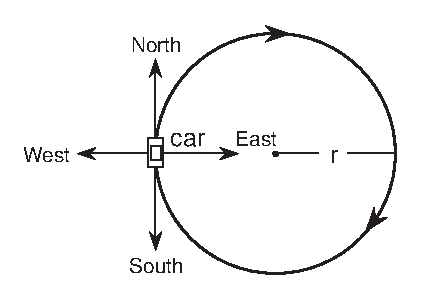
\includegraphics[keepaspectratio,scale=0.66]{June2007-Q04}
    %\begin{tikzpicture}
    %% NOTE: tikz
    %\end{tikzpicture}
    \end{center}
    When the car is in the position shown,
        its acceleration is directed toward the:
    \begin{multicols}{2}
    \begin{choices}
      \correctchoice{east}
        \wrongchoice{west}
        \wrongchoice{south}
        \wrongchoice{north}
    \end{choices}
    \end{multicols}
\end{question}
}

\element{nysed}{
\begin{question}{Jan2007-Q06}
    A ball attached to a string is moved at constant speed in a horizontal circular path.
    A target is located near the path of the ball as shown in the diagram.
    \begin{center}
    \begin{tikzpicture}
        %% Circle
        \draw (0,0) circle (2cm);
        %% Ball and string
        \draw[] (0:0cm) -- (120:2cm) node[anchor=south east] {ball};
        \draw[fill=white] (120:2cm) circle (3pt);
        %% Labels
        \draw[fill] (90:2cm) circle (2pt) node[anchor=south] {$A$};
        \draw[fill] (60:2cm) circle (2pt) node[anchor=south west] {$B$};
        \draw[fill] (-30:2cm) circle (2pt) node[anchor=north west] {$C$};
        \draw[fill] (270:2cm) circle (2pt) node[anchor=north] {$D$};
        %% Target
        %% NOTE: TODO: TARGET NOT finished
        \node[] at (-30:3cm) {target};
        %\draw rectangle
    \end{tikzpicture}
    \end{center}
    At which point along the ball's path should the string be released,
        if the ball is to hit the target?
    \begin{multicols}{4}
    \begin{choices}[o]
        \wrongchoice{$A$}
      \correctchoice{$B$}
        \wrongchoice{$C$}
        \wrongchoice{$D$}
    \end{choices}
    \end{multicols}
\end{question}
}

\element{nysed}{
\begin{question}{June2007-Q08}
    A \SI{0.50}{\kilo\gram} object moves in a horizontal circular path with a radius of \SI{0.25}{\meter} at a constant speed of \SI{4.0}{\meter\per\second}.
    What is the magnitude of the object's acceleration?
    \begin{multicols}{2}
    \begin{choices}
      \correctchoice{\SI{64}{\meter\per\second}}
        \wrongchoice{\SI{8.0}{\meter\per\second}}
        \wrongchoice{\SI{32}{\meter\per\second}}
        \wrongchoice{\SI{16}{\meter\per\second}}
    \end{choices}
    \end{multicols}
\end{question}
}


%% Section Jan2007
%%--------------------


%% Section June2006
%%--------------------
\element{nysed}{
\begin{question}{June2006-Q07}
    The diagram below shows the top view of a \SI{65}{\kilo\gram} student at point $A$ on an amusement park ride.
    The ride spins the student in a horizontal circle of radius \SI{2.5}{\meter}, at a constant speed of \SI{8.6}{\meter\per\second}.
    The floor is lowered and the student remains against the wall without falling to the floor.
    \begin{center}
        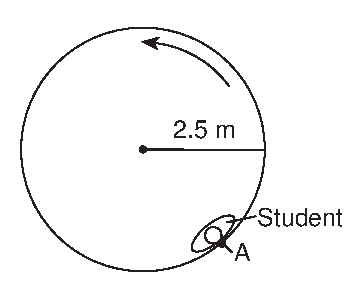
\includegraphics[keepaspectratio,scale=0.8]{June2006-Q07}
    \end{center}
    Which vector best represents the direction of the centripetal acceleration of the student at point $A$?
    \begin{multicols}{2}
    \begin{choices}
        \AMCboxDimensions{down=-0.4cm}
        \correctchoice{
            \begin{tikzpicture}
                \draw[dashed,white!90!black] (0,0) -- (1,1);
                \draw[thick,->] (0.85,0.15) -- (0.15,0.85);
            \end{tikzpicture}
        }
        \wrongchoice{
            \begin{tikzpicture}
                \draw[dashed,white!90!black] (0,0) -- (1,1);
                \draw[thick,->] (0.85,0.85) -- (0.15,0.15);
            \end{tikzpicture}
        }
        \wrongchoice{
            \begin{tikzpicture}
                \draw[dashed,white!90!black] (0,0) -- (1,1);
                \draw[thick,->] (0.15,0.85) -- (0.85,0.15);
            \end{tikzpicture}
        }
        \wrongchoice{
            \begin{tikzpicture}
                \draw[dashed,white!90!black] (0,0) -- (1,1);
                \draw[thick,->] (0.15,0.15) -- (0.85,0.85);
            \end{tikzpicture}
        }
    \end{choices}
    \end{multicols}
\end{question}
}

\element{nysed}{
\begin{question}{June2006-Q08}
    The diagram below shows the top view of a \SI{65}{\kilo\gram} student at point $A$ on an amusement park ride.
    The ride spins the student in a horizontal circle of radius \SI{2.5}{\meter}, at a constant speed of \SI{8.6}{\meter\per\second}.
    The floor is lowered and the student remains against the wall without falling to the floor.
    \begin{center}
        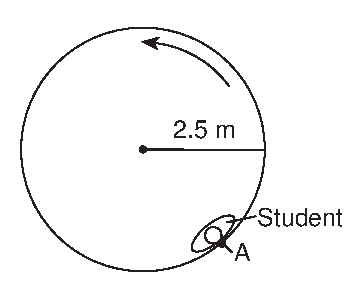
\includegraphics[keepaspectratio,scale=0.8]{June2006-Q07}
    \end{center}
    The magnitude of the centripetal force acting on the student at point $A$ is approximately:
    \begin{multicols}{2}
    \begin{choices}
      \correctchoice{\SI{1.9e3}{\newton}}
        \wrongchoice{\SI{1.2e4}{\newton}}
        \wrongchoice{\SI{2.2e2}{\newton}}
        \wrongchoice{\SI{3.0e1}{\newton}}
    \end{choices}
    \end{multicols}
\end{question}
}


%% Section Jan2006
%%--------------------
\element{nysed}{
\begin{question}{Jan2006-Q14}
    The diagram below shows a \SI{5.0}{\kilo\gram} bucket of water being swung in a horizontal circle of \SI{0.70}{\meter} radius at a constant speed of \SI{2.0}{\meter\per\second}
    \begin{center}
        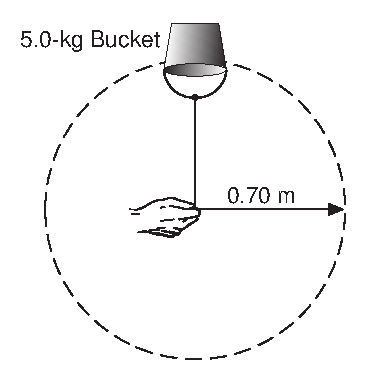
\includegraphics[keepaspectratio,scale=0.75]{Jan2006-Q14}
    \end{center}
    The magnitude of the centripetal force on the buck of water is approximately:
    \begin{multicols}{2}
    \begin{choices}
      \correctchoice{\SI{29}{\newton}}
        \wrongchoice{\SI{14}{\newton}}
        \wrongchoice{\SI{5.7}{\newton}}
        \wrongchoice{\SI{200}{\newton}}
    \end{choices}
    \end{multicols}
\end{question}
}

\element{nysed}{
\begin{question}{Jan2006-Q40}
    In the diagram below, a cart travels clockwise at constant speed in a horizontal circle.
    \begin{center}
        %% NOTE: tikzpicture
        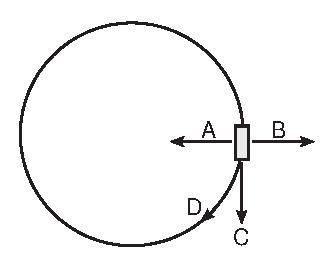
\includegraphics[keepaspectratio,scale=0.8]{Jan2006-Q40}
    \end{center}
    At the position shown in the diagram,
        which arrow indicates the direction of the centripetal acceleration?
    \begin{multicols}{2}
    \begin{choices}
      \correctchoice{$A$}
        \wrongchoice{$B$}
        \wrongchoice{$C$}
        \wrongchoice{$D$}
    \end{choices}
    \end{multicols}
\end{question}
}


%% Section June2005
%%--------------------
\element{nysed}{
\begin{question}{June2005-Q38}
    In the diagram below, $S$ is a point on a car tire rotating at a constant rate.
    \begin{center}
        \includegraphics[keepaspectratio,scale=0.8]{June2005-Q38}
    \end{center}
    Which graph best represents the magnitude of the centripetal acceleration of point $S$ as a function of time?
    \begin{multicols}{2}
    \begin{choices}
        \AMCboxDimensions{down=-2.5em}
        \correctchoice{
            \begin{tikzpicture}
                \begin{axis}[
                    axis y line=left,
                    axis x line=bottom,
                    axis line style={->},
                    xlabel={time},
                    xtick=\empty,
                    ylabel={acceleration},
                    ytick=\empty,
                    xmin=0,xmax=11,
                    ymin=0,ymax=11,
                    width=\columnwidth,
                    very thin,
                ]
                \addplot[line width=1pt,domain=0:10]{8};
                \end{axis}
            \end{tikzpicture}
        }
        \wrongchoice{
            \begin{tikzpicture}
                \begin{axis}[
                    axis y line=left,
                    axis x line=bottom,
                    axis line style={->},
                    xlabel={time},
                    xtick=\empty,
                    ylabel={acceleration},
                    ytick=\empty,
                    xmin=0,xmax=11,
                    ymin=0,ymax=11,
                    width=\columnwidth,
                    very thin,
                ]
                \addplot[line width=1pt,domain=0:10]{x};
                \end{axis}
            \end{tikzpicture}
        }
        \wrongchoice{
            \begin{tikzpicture}
                \begin{axis}[
                    axis y line=left,
                    axis x line=bottom,
                    axis line style={->},
                    xlabel={time},
                    xtick=\empty,
                    ylabel={acceleration},
                    ytick=\empty,
                    xmin=0,xmax=11,
                    ymin=0,ymax=11,
                    width=\columnwidth,
                    very thin,
                ]
                \addplot[line width=1pt,domain=0:10]{5/x};
                \end{axis}
            \end{tikzpicture}
        }
        \wrongchoice{
            \begin{tikzpicture}
                \begin{axis}[
                    axis y line=left,
                    axis x line=bottom,
                    axis line style={->},
                    xlabel={time},
                    xtick=\empty,
                    ylabel={acceleration},
                    ytick=\empty,
                    xmin=0,xmax=11,
                    ymin=0,ymax=11,
                    width=\columnwidth,
                    very thin,
                ]
                \addplot[line width=1pt,domain=0:10]{10 - 0.1*(10-x)*(10-x)};
                \end{axis}
            \end{tikzpicture}
        }
    \end{choices}
    \end{multicols}
\end{question}
}

\element{nysed}{
\begin{question}{June2005-Q46}
    A \SI{1.0e3}{\kilo\gram} car travels at a constant speed of \SI{20}{\meter\per\second} around a horizontal circular track.
    Which diagram correctly represents the direction of the car's velocity ($v$) and the direction of the centripetal force ($F_e$) acting on the car at one particular moment?
    \begin{multicols}{2}
    \begin{choices}
        %% NOTE: tikzpicture
      \correctchoice{\includegraphics[keepaspectratio,scale=0.66]{June2005-Q46-A}}
        \wrongchoice{\includegraphics[keepaspectratio,scale=0.66]{June2005-Q46-B}}
        \wrongchoice{\includegraphics[keepaspectratio,scale=0.66]{June2005-Q46-C}}
        \wrongchoice{\includegraphics[keepaspectratio,scale=0.66]{June2005-Q46-D}}
    \end{choices}
    \end{multicols}
\end{question}
}


%% Section Jan2005
%%--------------------


%% Section June2004
%%--------------------


%% Section Jan2004
%%--------------------
\element{nysed}{
\begin{question}{Jan2004-Q08}
    $A$ ball of mass $M$ at the end of a string is swung in a horizontal circular path of radius $R$ at constant speed $V$.
    Which combination of changes would require the greatest increase in the centripetal force acting on the ball?
    \begin{choices}
        \wrongchoice{doubling $V$ and doubling $R$}
      \correctchoice{doubling $V$ and halving $R$}
        \wrongchoice{halving $V$ and doubling $R$}
        \wrongchoice{halving $V$ and halving $R$}
    \end{choices}
\end{question}
}


%% Section June2003
%%--------------------
\element{nysed}{
\begin{question}{June2003-Q16}
    A child is riding on merry-go-round.
    As the speed of the merry-go-round is doubled,
        the magnitude of the centripetal force acting on the child:
    \begin{multicols}{2}
    \begin{choices}
      \correctchoice{remains the same}
        \wrongchoice{is doubled}
        \wrongchoice{is halved}
        \wrongchoice{is quadrupled}
    \end{choices}
    \end{multicols}
\end{question}
}


%% Section Jan2003
%%--------------------
\element{nysed}{
\begin{question}{Jan2003-Q09}
    A \SI{2.0e3}{\kilo\gram} car travels at a constant speed of \SI{12}{\meter\per\second} around a circular curve of radius \SI{30}{\meter}.
    What is the magnitude of the centripetal acceleration of the car as it goes around the curve?
    \begin{multicols}{2}
    \begin{choices}
      \correctchoice{\SI{4.8}{\meter\per\second\squared}}
        \wrongchoice{\SI{0.40}{\meter\per\second\squared}}
        \wrongchoice{\SI{800}{\meter\per\second\squared}}
        \wrongchoice{\SI{9600}{\meter\per\second\squared}}
    \end{choices}
    \end{multicols}
\end{question}
}

\element{nysed}{
\begin{question}{Jan2003-Q10}
    A \SI{2.0e3}{\kilo\gram} car travels at a constant speed of \SI{12}{\meter\per\second} around a circular curve of radius \SI{30}{\meter}.
    As the car goes around the curve, the centripetal force is directed:
    \begin{choices}
      \correctchoice{toward the center of the circular curve}
        \wrongchoice{away from the center of the circular curve}
        \wrongchoice{tangent to the curve in the direction of motion}
        \wrongchoice{tangent to the curve opposite the direction of motion}
    \end{choices}
\end{question}
}


%% Section Aug2002
%%--------------------
\element{nysed}{
\begin{question}{Aug2002-Q04}
    The diagram below represents a \SI{0.4}{\kilo\gram} stone attached to a string.
    The stone is moving at a constant speed of \SI{4.0}{\meter\per\second} in a horizontal circle having a radius of \SI{0.8}{\meter}.
    \begin{center}
    %% TODO: NOTE: insert graphic
    \begin{tikzpicture}
        \draw[thick,dashed] (0,0) circle (2cm);
        %\draw[thick,->] (170:2cm) arc (170:170:2cm);
        \draw[thick] (0,0) -- (160:2cm)
            node[pos=0.5,anchor=south west] {$r=\SI{0.80}{\meter}$};
        \draw[fill] (160:2cm) circle (4pt);
        \draw[thick,->] (160:2cm) -- ++(250:0.75cm);
        \node[anchor=south] at (-3.2,0.7) {$m=\SI{0.40}{\kilo\gram}$};
        \node[anchor=north] at (-3.2,0.7) {$v=\SI{4.0}{\meter\per\second}$};
    \end{tikzpicture}
    \end{center}
    The magnitude of the centripetal acceleration of the stone is:
    \begin{multicols}{2}
    \begin{choices}
        \wrongchoice{\SI{0.0}{\meter\per\second\squared}}
        \wrongchoice{\SI{2.0}{\meter\per\second\squared}}
        \wrongchoice{\SI{5.0}{\meter\per\second\squared}}
      \correctchoice{\SI{20}{\meter\per\second\squared}}
    \end{choices}
    \end{multicols}
\end{question}
}


%% Section June2002
%%--------------------
\element{nysed}{
\begin{question}{June2002-Q08}
    The diagram shows a student seated on a rotating circular platform,
    holding a \SI{2.0}{\kilo\gram} block with a spring scale.
    The block is \SI{1.2}{\meter} from the center of the platform.
    The block has a constant speed of \SI{8.0}{\meter\per\second}.
    [Frictional forces on the block are negligible.]
    \begin{center}
        \includegraphics[keepaspectratio,scale=1.0]{June2002-Q08}
    \end{center}
    Which statement best describes the block's movement as the platform rotates?
    \begin{choices}
      \correctchoice{Its velocity is directed tangent to the circular path, with an inward acceleration.}
        \wrongchoice{Its velocity is directed tangent to the circular path, with an outward acceleration.}
        \wrongchoice{Its velocity is directed perpendicular to the circular path, with an inward acceleration.}
        \wrongchoice{Its velocity is directed perpendicular to the circular path, with an outward acceleration.}
    \end{choices}
\end{question}
}

\element{nysed}{
\begin{question}{June2002-Q09}
    The diagram shows a student seated on a rotating circular platform,
    holding a \SI{2.0}{\kilo\gram} block with a spring scale.
    The block is \SI{1.2}{\meter} from the center of the platform.
    The block has a constant speed of \SI{8.0}{\meter\per\second}.
    [Frictional forces on the block are negligible.]
    \begin{center}
        \includegraphics[keepaspectratio,scale=1.0]{June2002-Q08}
    \end{center}
    The reading on the spring scale is approximately:
    \begin{multicols}{2}
    \begin{choices}
        \wrongchoice{\SI{20}{\newton}}
      \correctchoice{\SI{110}{\newton}}
        \wrongchoice{\SI{53}{\newton}}
        \wrongchoice{\SI{130}{\newton}}
    \end{choices}
    \end{multicols}
\end{question}
}


%% Section Jan2002
%%--------------------
\element{nysed}{
\begin{question}{Jan2002-Q59}
    A \SI{60}{\kilo\gram} car travels clockwise in a horizontal circle of radius \SI{10}{\meter} at \SI{5.0}{\meter\per\second}.
    \begin{center}
        \includegraphics[keepaspectratio,scale=0.8]{Jan2002-Q59}
    \end{center}
    The centripetal acceleration of the car at the position shown is directed toward point:
    \begin{multicols}{2}
    \begin{choices}[o]
        \wrongchoice{$A$}
        \wrongchoice{$B$}
      \correctchoice{$C$}
        \wrongchoice{$D$}
    \end{choices}
    \end{multicols}
\end{question}
}

\element{nysed}{
\begin{question}{Jan2002-Q60}
    A \SI{60}{\kilo\gram} car travels clockwise in a horizontal circle of radius \SI{10}{\meter} at \SI{5.0}{\meter\per\second}.
    \begin{center}
        \includegraphics[keepaspectratio,scale=0.8]{Jan2002-Q59}
    \end{center}
    The magnitude of the centripetal force acting on the car is:
    \begin{multicols}{2}
    \begin{choices}
        \wrongchoice{\SI{590}{\newton}}
      \correctchoice{\SI{150}{\newton}}
        \wrongchoice{\SI{30}{\newton}}
        \wrongchoice{\SI{2.5}{\newton}}
    \end{choices}
    \end{multicols}
\end{question}
}


%% Section June2001
%%--------------------
\element{nysed}{
\begin{question}{June2001-Q60}
    A \SI{1200}{\kilo\gram} car traveling at a constant speed of \SI{9.0}{\meter\per\second} turns at an intersection.
    The car follows a horizontal circular path with a radius of \SI{25}{\meter} to point $P$.
    \begin{center}
        \includegraphics[keepaspectratio,scale=0.9]{June2001-Q60}
    \end{center}
    The magnitude of the centripetal force acting on the car as it travels around the circular path is approximately:
    \begin{multicols}{2}
    \begin{choices}
        \wrongchoice{\SI{1.1e4}{\newton}}
        \wrongchoice{\SI{1.2e4}{\newton}}
      \correctchoice{\SI{3.9e3}{\newton}}
        \wrongchoice{\SI{4.3e2}{\newton}}
    \end{choices}
    \end{multicols}
\end{question}
}

\element{nysed}{
\begin{question}{June2001-Q61}
    A \SI{1200}{\kilo\gram} car traveling at a constant speed of \SI{9.0}{\meter\per\second} turns at an intersection.
    The car follows a horizontal circular path with a radius of \SI{25}{\meter} to point $P$.
    \begin{center}
        \includegraphics[keepaspectratio,scale=0.9]{June2001-Q60}
    \end{center}
    At point $P$, the car hits an area of ice and loses all frictional force on its tires.
    Which path does the car follow on the ice?
    \begin{multicols}{4}
    \begin{choices}[o]
        \wrongchoice{$A$}
      \correctchoice{$B$}
        \wrongchoice{$C$}
        \wrongchoice{$D$}
    \end{choices}
    \end{multicols}
\end{question}
}

\element{nysed}{
\begin{question}{June2001-Q62}
    An amusement park ride moves a rider at a constant speed of \SI{14}{\meter\per\second} in a horizontal circular path of radius \SI{10}{\meter}.
    What is the rider's centripetal acceleration in terms of $g$,
        the acceleration due to gravity?
    \begin{multicols}{4}
    \begin{choices}
        \wrongchoice{$1g$}
      \correctchoice{$2g$}
        \wrongchoice{$3g$}
        \wrongchoice{$0g$}
    \end{choices}
    \end{multicols}
\end{question}
}


%% Section Jan2001
%%--------------------
\element{nysed}{
\begin{question}{Jan2001-Q56}
    A \SI{1.00e3}{\kilo\gram} car is driven clockwise around a flat circular track of radius \SI{25.0}{\meter}.
    The speed of the car is a constant \SI{5.00}{\meter\per\second}.
    \begin{center}
        \includegraphics[keepaspectratio,scale=0.8]{Jan2001-Q56}
    \end{center}
    What minimum friction force must exist between the tires and the road to prevent the car from skidding as it rounds the curve?
    \begin{multicols}{2}
    \begin{choices}
        \wrongchoice{\SI{1.25e5}{\newton}}
        \wrongchoice{\SI{9.80e4}{\newton}}
        \wrongchoice{\SI{5.00e3}{\newton}}
      \correctchoice{\SI{1.00e3}{\newton}}
    \end{choices}
    \end{multicols}
\end{question}
}

\element{nysed}{
\begin{question}{Jan2001-Q57}
    A \SI{1.00e3}{\kilo\gram} car is driven clockwise around a flat circular track of radius \SI{25.0}{\meter}.
    The speed of the car is a constant \SI{5.00}{\meter\per\second}.
    \begin{center}
        \includegraphics[keepaspectratio,scale=0.8]{Jan2001-Q56}
    \end{center}
    If the circular track were to suddenly become frictionless at the instant shown in the diagram,
        the car's direction of travel would be:
    \begin{multicols}{2}
    \begin{choices}
        \wrongchoice{toward E}
      \correctchoice{toward N}
        \wrongchoice{toward W}
        \wrongchoice{a clockwise spiral}
    \end{choices}
    \end{multicols}
\end{question}
}

\element{nysed}{
\begin{question}{Jan2001-Q57}
    A \SI{1.00e3}{\kilo\gram} car is driven clockwise around a flat circular track of radius \SI{25.0}{\meter}.
    The speed of the car is a constant \SI{5.00}{\meter\per\second}.
    \begin{center}
        \includegraphics[keepaspectratio,scale=0.8]{Jan2001-Q56}
    \end{center}
    If the circular track were to suddenly become frictionless at the instant shown in the diagram,
        the car's direction of travel would be:
    \begin{multicols}{2}
    \begin{choices}
        \wrongchoice{toward E}
      \correctchoice{toward N}
        \wrongchoice{toward W}
        \wrongchoice{a clockwise spiral}
    \end{choices}
    \end{multicols}
\end{question}
}

\element{nysed}{
\begin{question}{Jan2001-Q58}
    A \SI{1.00e3}{\kilo\gram} car is driven clockwise around a flat circular track of radius \SI{25.0}{\meter}.
    The speed of the car is a constant \SI{5.00}{\meter\per\second}.
    \begin{center}
        \includegraphics[keepaspectratio,scale=0.8]{Jan2001-Q56}
    \end{center}
    At the instant shown in the diagram,
        the car's centripetal acceleration is directed:
    \begin{multicols}{2}
    \begin{choices}
      \correctchoice{toward E}
        \wrongchoice{toward N}
        \wrongchoice{toward W}
        \wrongchoice{clockwise}
    \end{choices}
    \end{multicols}
\end{question}
}

\element{nysed}{
\begin{question}{Jan2001-Q59}
    A \SI{1.00e3}{\kilo\gram} car is driven clockwise around a flat circular track of radius \SI{25.0}{\meter}.
    The speed of the car is a constant \SI{5.00}{\meter\per\second}.
    \begin{center}
        \includegraphics[keepaspectratio,scale=0.8]{Jan2001-Q56}
    \end{center}
    Which factor, when doubled, would produce the greatest change in the centripetal force acting on the car?
    \begin{multicols}{2}
    \begin{choices}
        \wrongchoice{mass of the car}
        \wrongchoice{radius of the track}
      \correctchoice{velocity of the car}
        \wrongchoice{weight of the car}
    \end{choices}
    \end{multicols}
\end{question}
}


%% Section June2000
%%--------------------
\element{nysed}{
\begin{question}{June2000-Q60}
    As a cart travels around a horizontal circular track,
        the cart \emph{must} undergo a change in:
    \begin{multicols}{2}
    \begin{choices}
      \correctchoice{velocity}
        \wrongchoice{inertia}
        \wrongchoice{speed}
        \wrongchoice{weight}
    \end{choices}
    \end{multicols}
\end{question}
}

\element{nysed}{
\begin{question}{June2000-Q64}
    A ball attached to a string is whirled at a constant speed of \SI{2.0}{\meter\per\second} in a horizontal circle of radius \SI{0.50}{\meter}.
    What is the magnitude of the ball's centripetal acceleration?
    \begin{multicols}{2}
    \begin{choices}
        \wrongchoice{\SI{1.0}{\meter\per\second\squared}}
        \wrongchoice{\SI{2.0}{\meter\per\second\squared}}
      \correctchoice{\SI{8.0}{\meter\per\second\squared}}
        \wrongchoice{\SI{4.0}{\meter\per\second\squared}}
    \end{choices}
    \end{multicols}
\end{question}
}


%% Section June1999
%%--------------------
\newcommand{\JuneNineteenNinetyNineQSixtyThree}{
\begin{tikzpicture}
    %% Circle
    \draw[dashed] (0,0) circle (2cm);
    %% Arrows
    \foreach \x in {45,135,225,315} \draw[black,thick,->] (\x:2) arc(\x:{\x-5}:2);
    \draw[thick,-latex] (0,0) -- (30:2) node[pos=0.4,anchor=north west] {\SI{2.0}{\meter}};
    \node[anchor=north] at (0,-2) {top view};
    %% options
    \fill (-2,0) ++(90:1.5) circle (2pt) node[anchor=south] {$B$};
    \fill (-2,0) ++(180:1) circle (2pt) node[anchor=south] {$C$};
    \fill (-2,0) ++(270:1.5) circle (2pt) node[anchor=north] {$D$};
    \fill (-2,0) ++(0:1) circle (2pt) node[anchor=south] {$A$};
    %% Rock and directions
    \fill (180:2) circle (1ex);
    \node[pin={[text width=4em,pin edge={latex-,shorten <=1mm}]225:{\SI{7.0}{\kilo\gram} hammer}}] at (180:2) {};
    \draw[very thick,->] (0,0) -- (180:2);
\end{tikzpicture}
}

\element{nysed}{
\begin{question}{June1999-Q63}
    An athlete in a hammer-throw event swings a \SI{7.0}{\kilo\gram} hammer in a horizontal circle at a constant speed of \SI{12}{\meter\per\second}.
    The radius of the hammer's path is \SI{2.0}{\meter}.
    \begin{center}
        \JuneNineteenNinetyNineQSixtyThree
    \end{center}
    At the position shown,
        the centripetal force acting on the hammer is directed toward point:
    \begin{multicols}{4}
    \begin{choices}[o]
      \correctchoice{$A$}
        \wrongchoice{$B$}
        \wrongchoice{$C$}
        \wrongchoice{$D$}
    \end{choices}
    \end{multicols}
\end{question}
}

\element{nysed}{
\begin{question}{June1999-Q64}
    An athlete in a hammer-throw event swings a \SI{7.0}{\kilo\gram} hammer in a horizontal circle at a constant speed of \SI{12}{\meter\per\second}.
    The radius of the hammer's path is \SI{2.0}{\meter}.
    \begin{center}
        \JuneNineteenNinetyNineQSixtyThree
    \end{center}
    What is the magnitude of the centripetal acceleration of the hammer?
    \begin{multicols}{2}
    \begin{choices}
        \wrongchoice{\SI{6.0}{\meter\per\second\squared}}
        \wrongchoice{\SI{24}{\meter\per\second\squared}}
      \correctchoice{\SI{72}{\meter\per\second\squared}}
        \wrongchoice{\SI{500}{\meter\per\second\squared}}
    \end{choices}
    \end{multicols}
\end{question}
}

\element{nysed}{
\begin{question}{June1999-Q66}
    An athlete in a hammer-throw event swings a \SI{7.0}{\kilo\gram} hammer in a horizontal circle at a constant speed of \SI{12}{\meter\per\second}.
    The radius of the hammer's path is \SI{2.0}{\meter}.
    \begin{center}
        \JuneNineteenNinetyNineQSixtyThree
    \end{center}
    If the hammer is released at the position shown,
        it will travel toward point:
    \begin{multicols}{4}
    \begin{choices}[o]
        \wrongchoice{$A$}
      \correctchoice{$B$}
        \wrongchoice{$C$}
        \wrongchoice{$D$}
    \end{choices}
    \end{multicols}
\end{question}
}


%% Section June1998
%%--------------------

%% NOTE: June1998-Q58 requires graphic, tikz?
%% NOTE: June1998-Q59 same as Q58
%% NOTE: June1998-Q60 same as Q58
\newcommand{\JuneNineteenNinetyNineQFiftyEight}{
\begin{tikzpicture}
    %% path
\end{tikzpicture}
}

\element{nysed}{
\begin{question}{June1998-Q59}
    The diagram below shows a \SI{2.0}{\kilo\gram} cart traveling at a constant speed in a horizontal circle of radius \SI{3.0}{\meter}.
    The magnitude of the centripetal force of the cart is \SI{24}{\newton}.
    \begin{center}
        \JuneNineteenNinetyNineQFiftyEight
    \end{center}
    In the position shown, the acceleration of the cart is:
    \begin{choices}
        \wrongchoice{\SI{8.0}{\meter\per\second\squared} directed toward point $A$}
        \wrongchoice{\SI{8.0}{\meter\per\second\squared} directed toward point $D$}
        \wrongchoice{\SI{12.0}{\meter\per\second\squared} directed toward point $A$}
        \wrongchoice{\SI{12.0}{\meter\per\second\squared} directed toward point $D$}
    \end{choices}
\end{question}
}

\element{nysed}{
\begin{question}{June1998-Q60}
    The diagram below shows a \SI{2.0}{\kilo\gram} cart traveling at a constant speed in a horizontal circle of radius \SI{3.0}{\meter}.
    The magnitude of the centripetal force of the cart is \SI{24}{\newton}.
    \begin{center}
        \JuneNineteenNinetyNineQFiftyEight
    \end{center}
    Which statement correctly describes the direction of the cart's velocity and centripetal force in the position shown?
    \begin{choices}
        \wrongchoice{velocity is directed toward point $B$, and the centripetal force is directed toward point $A$}
        \wrongchoice{velocity is directed toward point $B$, and the centripetal force is directed toward point $D$}
        \wrongchoice{velocity is directed toward point $C$, and the centripetal force is directed toward point $A$}
        \wrongchoice{velocity is directed toward point $C$, and the centripetal force is directed toward point $D$}
    \end{choices}
\end{question}
}

\element{nysed}{
\begin{question}{June1998-Q61}
    The diagram below shows a \SI{2.0}{\kilo\gram} cart traveling at a constant speed in a horizontal circle of radius \SI{3.0}{\meter}.
    The magnitude of the centripetal force of the cart is \SI{24}{\newton}.
    \begin{center}
        \JuneNineteenNinetyNineQFiftyEight
    \end{center}
    What is the speed of the cart?
    \begin{multicols}{2}
    \begin{choices}
        \wrongchoice{\SI{6.0}{\meter\per\second}}
        \wrongchoice{\SI{16}{\meter\per\second}}
        \wrongchoice{\SI{36}{\meter\per\second}}
        \wrongchoice{\SI{4.0}{\meter\per\second}}
    \end{choices}
    \end{multicols}
\end{question}
}


%% Section June1997
%%--------------------
\element{nysed}{
\begin{question}{June1997-Q07}
    A ball rolls through a hollow semicircular tube lying flat on a horizontal tabletop.
    Which diagram shows the path of the ball after emerging from the tube,
        as viewed from above?
    \begin{multicols}{2}
    \begin{choices}
        \AMCboxDimensions{down=-1cm}
        \wrongchoice{
            \begin{tikzpicture}
                %% table top
                \draw[dashed,white!60!black] (-1.5,-2.5) rectangle (1.5,1.5);
                \node[anchor=south] at (0,-2.5) {Tabletop};
                %% loop
                \draw (0,1.2) arc (90:270:1.2) arc(270:90:0.05 and 0.1) arc(270:90:1.0) arc(270:90:0.05 and 0.1) -- cycle;
                \draw (0,-1.1) circle (0.05 and 0.1);
                \draw (0,+1.1) circle (0.05 and 0.1);
                %% ball and vector
                \fill (0.05,-1.1) circle (0.04 and 0.08);
                \draw[thick,->] (0,-1.1) arc(270:360:1.1);
            \end{tikzpicture}
        }
        \wrongchoice{
            \begin{tikzpicture}
                %% table top
                \draw[dashed,white!60!black] (-1.5,-2.5) rectangle (1.5,1.5);
                \node[anchor=south] at (0,-2.5) {Tabletop};
                %% loop
                \draw (0,1.2) arc (90:270:1.2) arc(270:90:0.05 and 0.1) arc(270:90:1.0) arc(270:90:0.05 and 0.1) -- cycle;
                \draw (0,-1.1) circle (0.05 and 0.1);
                \draw (0,+1.1) circle (0.05 and 0.1);
                %% ball and vector
                \fill (0.05,-1.1) circle (0.04 and 0.08);
                \draw[thick,->] (0,-1.1) arc(90:0:1.1);
            \end{tikzpicture}
        }
        \wrongchoice{
            \begin{tikzpicture}
                %% table top
                \draw[dashed,white!60!black] (-1.5,-2.5) rectangle (1.5,1.5);
                \node[anchor=south] at (0,-2.5) {Tabletop};
                %% loop
                \draw (0,1.2) arc (90:270:1.2) arc(270:90:0.05 and 0.1) arc(270:90:1.0) arc(270:90:0.05 and 0.1) -- cycle;
                \draw (0,-1.1) circle (0.05 and 0.1);
                \draw (0,+1.1) circle (0.05 and 0.1);
                %% ball and vector
                \fill (0.05,-1.1) circle (0.04 and 0.08);
                \draw[thick,->] (0,-1.1) -- ++(270:0.8);
            \end{tikzpicture}
        }
        %% Newton's first law
        \correctchoice{
            \begin{tikzpicture}
                %% table top
                \draw[dashed,white!60!black] (-1.5,-2.5) rectangle (1.5,1.5);
                \node[anchor=south] at (0,-2.5) {Tabletop};
                %% loop
                \draw (0,1.2) arc (90:270:1.2) arc(270:90:0.05 and 0.1) arc(270:90:1.0) arc(270:90:0.05 and 0.1) -- cycle;
                \draw (0,-1.1) circle (0.05 and 0.1);
                \draw (0,+1.1) circle (0.05 and 0.1);
                %% ball and vector
                \fill (0.05,-1.1) circle (0.04 and 0.08);
                \draw[thick,->] (0,-1.1) -- ++(0:1);
            \end{tikzpicture}
        }
    \end{choices}
    \end{multicols}
\end{question}
}

%% NOTE: Q58 to Q60 uses common graphic
%% NOTE: June1997-Q58 requires graphics
%% NOTE: June1997-Q59 requires graphics
%% NOTE: June1997-Q60 requires graphics


%% Section June1996
%%--------------------
\newcommand{\JuneOneNineNineSixQFiftyNine}{
\begin{tikzpicture}
    %% path
    \draw[dashed] (0,0) circle (3cm and 0.75cm);
    \draw[thick,->] (0,0) -- (180:3) node[pos=0.5,anchor=south] {string};
    %% arrows
    \foreach \x in {45,135,225,315}
        \draw[thick,-latex] ({3*cos(\x)},{0.75*sin(\x)}) arc(\x:{\x-10}:3 and 0.75);
    %% ball
    \fill (180:3) circle (2pt) node[anchor=east,xshift=-2pt] {ball};
    %% hand
    \draw[thick,->] (0,-1) -- (0,0) node[pos=0,anchor=north] {hand};
\end{tikzpicture}
}

\element{nysed}{
\begin{question}{June1996-Q59}
    The diagram shows a student spinning a \SI{0.10}{\kilo\gram} ball at the end of a \SI{0.50}{\meter} string in a horizontal circle at a constant speed of \SI{10}{\meter\per\second}.
    [Neglect air resistance.]
    \begin{center}
        %% NOTE: tikz?
        \JuneOneNineNineSixQFiftyNine
    \end{center}
    If the magnitude of the force applied to the string by the student's hand is increased,
        the magnitude of the acceleration of the ball in its circular path will:
    \begin{choices}
        \wrongchoice{decrease}
      \correctchoice{increase}
        \wrongchoice{remain the same}
    \end{choices}
\end{question}
}

\element{nysed}{
\begin{question}{June1996-Q60}
    The diagram shows a student spinning a \SI{0.10}{\kilo\gram} ball at the end of a \SI{0.50}{\meter} string in a horizontal circle at a constant speed of \SI{10}{\meter\per\second}.
    [Neglect air resistance.]
    \begin{center}
        \JuneOneNineNineSixQFiftyNine
    \end{center}
    The magnitude of the centripetal force required to keep the ball in this circular path is:
    \begin{multicols}{2}
    \begin{choices}
        \wrongchoice{\SI{5.0}{\newton}}
        \wrongchoice{\SI{10}{\newton}}
      \correctchoice{\SI{20}{\newton}}
        \wrongchoice{\SI{200}{\newton}}
    \end{choices}
    \end{multicols}
\end{question}
}

\element{nysed}{
\begin{question}{June1996-Q61}
    The diagram shows a student spinning a \SI{0.10}{\kilo\gram} ball at the end of a \SI{0.50}{\meter} string in a horizontal circle at a constant speed of \SI{10}{\meter\per\second}.
    [Neglect air resistance.]
    \begin{center}
        \JuneOneNineNineSixQFiftyNine
    \end{center}
    Which is the best description of the force keeping the ball in the circular path?
    \begin{choices}
      \correctchoice{perpendicular to the circle and directed toward the center of the circle}
        \wrongchoice{perpendicular to the circle and directed away from the center of the circle}
        \wrongchoice{tangent to the circle and directed in the same direction that the ball is moving}
        \wrongchoice{tangent to the circle and directed opposite to the direction that the ball is moving}
    \end{choices}
\end{question}
}

\element{nysed}{
\begin{question}{June1996-Q62}
    A convertible car with its top down is traveling at constant speed around a circular track,
        as shown in the diagram below.
    \begin{center}
    \begin{tikzpicture}
        %% track
        \draw (0,0) circle (2cm);
        %% car
        \draw[very thick,->] (0,-2) arc (270:300:2);
        \draw[fill=white!90!black] (-0.25,-1.9) rectangle (0.25,-2.1);
        \node[anchor=south] at (0,-1.9) {car};
        %% Options
        \fill (2,0) circle (2pt) node[anchor=west] {$A$};
        \fill (2,2) circle (2pt) node[anchor=west] {$C$};
        \fill (0,2) circle (2pt) node[anchor=north] {$B$};
        \fill (3,0) circle (2pt) node[anchor=south] {$D$};
    \end{tikzpicture}
    \end{center}
    When the car is at point $I$, if a passenger in the car throws a ball straight up,
        the ball could land at point:
    \begin{multicols}{4}
    \begin{choices}[o]
        \wrongchoice{$A$}
        \wrongchoice{$B$}
      \correctchoice{$C$}
        \wrongchoice{$D$}
    \end{choices}
    \end{multicols}
\end{question}
}


%% Section June1995
%%--------------------
\newcommand{\nysedJuneNineteenNinetyFiveQFiftyNine}{
\begin{tikzpicture}
    %% clockwise path
    \draw[dashed] (0,0) circle (2cm);
    \draw[thick,-latex] (0,0) -- (135:2) node[pos=0.5,anchor=south,rotate=-45] {\SI{2.0}{\meter}};
    \foreach \x in {100,220,340}
        \draw[thick,-latex] (\x:2) arc(\x:{\x-2}:2);
    %% Cart
    \node[minimum height=1ex,minimum width=0.66ex,draw,fill] (C) at (2,0) {};
    \node[anchor=west] at (C.east) {Cart};
    %% options
    \fill (0,0) circle (2pt) node[anchor=south west] {$Q$};
    \fill (4,0) circle (2pt) node[anchor=south west] {$R$};
    \fill (2,-2) circle (2pt) node[anchor=south west] {$S$};
    \fill (0,-2) circle (2pt) node[anchor=north west] {$P$};
\end{tikzpicture}
}

\element{nysed}{
\begin{question}{June1995-Q59}
    The diagram shows a \SI{5.0}{\kilo\gram} cart traveling clockwise in a horizontal circle of radius \SI{2.0}{\meter} at a constant speed of \SI{4.0}{\meter\per\second}.
    \begin{center}
        \nysedJuneNineteenNinetyFiveQFiftyNine
    \end{center}
    %% start question
    At the position show, the velocity of the cart is directed toward point?
    \begin{multicols}{4}
    \begin{choices}
        \wrongchoice{$P$}
        \wrongchoice{$Q$}
        \wrongchoice{$R$}
      \correctchoice{$S$}
    \end{choices}
    \end{multicols}
\end{question}
}

\element{nysed}{
\begin{question}{June1995-Q60}
    The diagram shows a \SI{5.0}{\kilo\gram} cart traveling clockwise in a horizontal circle of radius \SI{2.0}{\meter} at a constant speed of \SI{4.0}{\meter\per\second}.
    \begin{center}
        \nysedJuneNineteenNinetyFiveQFiftyNine
    \end{center}
    %% start question
    At the position show, the centripetal acceleration of the cart is directed toward point:
    \begin{multicols}{4}
    \begin{choices}
        \wrongchoice{$P$}
      \correctchoice{$Q$}
        \wrongchoice{$R$}
        \wrongchoice{$S$}
    \end{choices}
    \end{multicols}
\end{question}
}

\element{nysed}{
\begin{question}{June1995-Q61}
    The diagram shows a \SI{5.0}{\kilo\gram} cart traveling clockwise in a horizontal circle of radius \SI{2.0}{\meter} at a constant speed of \SI{4.0}{\meter\per\second}.
    \begin{center}
        \nysedJuneNineteenNinetyFiveQFiftyNine
    \end{center}
    %% start question
    If the mass of the cart was doubled,
        the magnitude of the centripetal acceleration of the cart would be:
    \begin{multicols}{2}
    \begin{choices}
      \correctchoice{unchanged}
        \wrongchoice{doubled}
        \wrongchoice{halved}
        \wrongchoice{quadrupled}
    \end{choices}
    \end{multicols}
\end{question}
}

\element{nysed}{
\begin{question}{June1995-Q62}
    The diagram shows a \SI{5.0}{\kilo\gram} cart traveling clockwise in a horizontal circle of radius \SI{2.0}{\meter} at a constant speed of \SI{4.0}{\meter\per\second}.
    \begin{center}
        \nysedJuneNineteenNinetyFiveQFiftyNine
    \end{center}
    %% start question
    What is the magnitude of the centripetal force acting on the cart?
    \begin{multicols}{2}
    \begin{choices}
        \wrongchoice{\SI{8.0}{\newton}}
        \wrongchoice{\SI{20}{\newton}}
      \correctchoice{\SI{40}{\newton}}
        \wrongchoice{\SI{50}{\newton}}
    \end{choices}
    \end{multicols}
\end{question}
}


%% Section June1994
%%--------------------


%% Section June1989
%%--------------------
\element{nysed}{
\begin{question}{June1989-Q62}
    Two masses, $A$ and $B$, move in circular path as shown in the diagram.
    \begin{center}
    \begin{tikzpicture}[scale=1.33]
        \fill (0,0) circle (2pt);
        %% A loop
        \fill (90:1.5) circle (2pt) node[anchor=south] {$A$};
        \draw[thick,-latex] (0,0) -- (45:1.5) node[pos=0.5,anchor=center,fill=white,rotate=-45] {\SI{1}{\meter}};
        \draw[very thick,-latex] (1.5,0) arc(0:120:1.5) node[pos=0.375,anchor=south,rotate=-45] {$v=\SI{2}{\meter\per\second}$};
        %% B loop
        \fill (140:3) circle (2pt) node[anchor=south east] {$B$};
        \draw[thick,-latex] (0,0) -- (135:3) node[pos=0.75,anchor=center,fill=white,rotate=45] {\SI{2}{\meter}};
        \draw[very thick,-latex] (45:3) arc(45:160:3);
        \node[anchor=south] at (0,3) {$v=\SI{2}{\meter\per\second}$};
    \end{tikzpicture}
    \end{center}
    The centripetal acceleration of mass $A$,
        compared to that of mass $B$, is:
    \begin{choices}
        \wrongchoice{the same}
      \correctchoice{twice as great}
        \wrongchoice{one-half as great}
        \wrongchoice{four times as great}
    \end{choices}
\end{question}
}

\element{nysed}{
\begin{question}{June1989-Q65}
    The diagram below shows an object traveling clockwise in a horizontal,
        circular path at constant speed.
    \begin{center}
    \begin{tikzpicture}
        \fill (0,0) circle (1.5pt);
        %% path
        \draw (0,0) circle (2cm);
        \draw[thick,->] (135:2.5) arc(135:80:2.5);
        \path[postaction={decoration={text along path, text={clockwise},text align=center},decorate}] (135:2.7) arc(135:80:2.7);
        \path[postaction={decoration={text along path, text={motion},text align=center},decorate}] (135:2.1) arc(135:80:2.1);
        %% object
        \draw[fill=white!60!black] (2,0) circle (5pt) node[anchor=west,xshift=5pt] {object};
    \end{tikzpicture}
    \end{center}
    Which arrow best shows the direction of the centripetal acceleration of the object at the instant shown?
    \begin{multicols}{2}
    \begin{choices}
        \AMCboxDimensions{down=-0.8cm}
        \correctchoice{
            \begin{tikzpicture}[scale=2]
                \draw[dashed,white!60!black] (0,0) rectangle (1,1);
                \draw[thick,->] (1,0.5) -- (0,0.5);
            \end{tikzpicture}
        }
        \wrongchoice{
            \begin{tikzpicture}[scale=2]
                \draw[dashed,white!60!black] (0,0) rectangle (1,1);
                \draw[thick,->] (0,0.5) -- (1,0.5);
            \end{tikzpicture}
        }
        \wrongchoice{
            \begin{tikzpicture}[scale=2]
                \draw[dashed,white!60!black] (0,0) rectangle (1,1);
                \draw[thick,->] (0.5,1) -- (0.5,0);
            \end{tikzpicture}
        }
        \wrongchoice{
            \begin{tikzpicture}[scale=2]
                \draw[dashed,white!60!black] (0,0) rectangle (1,1);
                \draw[thick,->] (0.5,0) -- (0.5,1);
            \end{tikzpicture}
        }
    \end{choices}
    \end{multicols}
\end{question}
}


\endinput



%
%% Internal Energy Questions used on the
%% NYSED Physics Regents Examination
%%--------------------------------------------------

%% this section contains 120 problems


%% NOTE: Jan2002 is the last exam to include Thermodynamics


%% Section Jan2002
%%--------------------
\element{nysed}{
\begin{question}{Jan2002-Q66}
    The diagram below represents an experiment in which a student placed a \SI{0.030}{\kilo\gram} lead cube in a beaker of water at \SI{20}{\degreeCelsius} and then heated the beaker until the water began to boil.
    \begin{center}
        \includegraphics[keepaspectratio,scale=0.75]{Jan2002-Q66}
    \end{center}
    The maximum amount of heat absorbed by the lead cube during the experiment was approximately:
    \begin{multicols}{2}
    \begin{choices}
      \correctchoice{\SI{0.31}{\kilo\joule}}
        \wrongchoice{\SI{10}{\kilo\joule}}
        \wrongchoice{\SI{60}{\kilo\joule}}
        \wrongchoice{\SI{790}{\kilo\joule}}
    \end{choices}
    \end{multicols}
\end{question}
}

\element{nysed}{
\begin{question}{Jan2002-Q67}
    Absolute zero is best described as the temperature at which:
    \begin{choices}
        \wrongchoice{water freezes at standard pressure}
        \wrongchoice{water is at its triple point}
        \wrongchoice{the molecules of a substance have maximum kinetic energy}
      \correctchoice{the molecules of a substance have minimum kinetic energy}
    \end{choices}
\end{question}
}

\element{nysed}{
\begin{question}{Jan2002-Q68}
    A temperature change of \SI{20}{\degreeCelsius} is equal to a temperature change of:
    \begin{multicols}{2}
    \begin{choices}
      \correctchoice{\SI{20}{\kelvin}}
        \wrongchoice{\SI{120}{\kelvin}}
        \wrongchoice{\SI{253}{\kelvin}}
        \wrongchoice{\SI{293}{\kelvin}}
    \end{choices}
    \end{multicols}
\end{question}
}

\element{nysed}{
\begin{question}{Jan2002-Q69}
    Heat will always flow from object $A$ to object $B$ if object $B$ has a lower:
    \begin{multicols}{2}
    \begin{choices}
        \wrongchoice{mass}
        \wrongchoice{total energy}
      \correctchoice{temperature}
        \wrongchoice{specific heat}
    \end{choices}
    \end{multicols}
\end{question}
}

\element{nysed}{
\begin{question}{Jan2002-Q70}
    Equal amounts of heat energy are given off by \SI{1.0}{\kilo\gram} samples of aluminum,
        iron, platinum, and zinc, all initially at \SI{100}{\degreeCelsius}.
    Which sample has the greatest decrease in temperature?
    %% TODO: add specific heats to ref.tex
    %% Specific Heats
    %% Al 0.91 kJ per kg per K
    %% Fe 0.45 kJ per kg per K
    %% Pa 0.13 kJ per kg per K
    %% Zn 0.39 kJ per kg per K
    \begin{multicols}{2}
    \begin{choices}
        \wrongchoice{aluminum}
        \wrongchoice{iron}
      \correctchoice{platinum}
        \wrongchoice{zinc}
    \end{choices}
    \end{multicols}
\end{question}
}

\element{nysed}{
\begin{question}{Jan2002-Q71}
    The graph below shows the temperature of \SI{3.0}{\kilo\gram} of a pure substance initially in the solid phase as heat is added to it at a constant rate.
    \begin{center}
    \begin{tikzpicture}
        \begin{axis}[
            axis y line=left, 
            axis x line=bottom, 
            axis line style={->},
            ylabel={temperature},
            y unit=\si{\degreeCelsius},
            ytick=\empty,
            xlabel={heat added},
            x unit=\si{\kilo\joule},
            xtick={0,75,150},
            ymin=0,ymax=400,
            xmin=0,xmax=225,
            width=0.8\columnwidth,
            height=0.5\columnwidth,
        ]
        \addplot[line width=1pt,mark=\empty] plot coordinates { (0,0) (75,200) (150,200) (225,400) };
        \draw[dashed] (axis cs:75,0) -- (axis cs:75,200);
        \draw[dashed] (axis cs:150,0) -- (axis cs:150,200);
        \end{axis}
    \end{tikzpicture}
    \end{center}
    The substance is most likely:
    \begin{multicols}{2}
    \begin{choices}
        \wrongchoice{alcohol}
        \wrongchoice{silver}
        \wrongchoice{copper}
      \correctchoice{lead}
    \end{choices}
    \end{multicols}
\end{question}
}

\element{nysed}{
\begin{question}{Jan2002-Q72}
    As a large quantity of salt is added to a container of boiling water, the water:
    \begin{choices}
        \wrongchoice{stops boiling because the boiling point decreases}
      \correctchoice{stops boiling because the boiling point increases}
        \wrongchoice{boils faster because the boiling point decreases}
        \wrongchoice{boils faster because the boiling point increases}
    \end{choices}
\end{question}
}

\element{nysed}{
\begin{question}{Jan2002-Q73}
    The total effect of all the processes that occur in the universe is an increase in:
    \begin{multicols}{2}
    \begin{choices}
      \correctchoice{entropy}
        \wrongchoice{temperature}
        \wrongchoice{order}
        \wrongchoice{energy}
    \end{choices}
    \end{multicols}
\end{question}
}

\element{nysed}{
\begin{question}{Jan2002-Q74}
    Which graph best represents the relationship between volume and absolute temperature for a fixed mass of an ideal gas at constant pressure?
    \begin{multicols}{2}
    \begin{choices}
        \AMCboxDimensions{down=-2.5em}
        \correctchoice{
            \begin{tikzpicture}
                \begin{axis}[
                    axis y line=left, 
                    axis x line=bottom, 
                    axis line style={->},
                    xlabel={temperature},
                    xtick=\empty,
                    ylabel={volume},
                    ytick=\empty,
                    xmin=0,xmax=11,
                    ymin=0,ymax=11,
                    width=\columnwidth,
                ]
                \addplot[line width=1pt,domain=0:10]{x};
                \end{axis}
            \end{tikzpicture}
        }
        \wrongchoice{
            \begin{tikzpicture}
                \begin{axis}[
                    axis y line=left, 
                    axis x line=bottom, 
                    axis line style={->},
                    xlabel={temperature},
                    xtick=\empty,
                    ylabel={volume},
                    ytick=\empty,
                    xmin=0,xmax=11,
                    ymin=0,ymax=11,
                    width=\columnwidth,
                ]
                \addplot[line width=1pt,domain=0:10]{10-x};
                \end{axis}
            \end{tikzpicture}
        }
        \wrongchoice{
            \begin{tikzpicture}
                \begin{axis}[
                    axis y line=left, 
                    axis x line=bottom, 
                    axis line style={->},
                    xlabel={temperature},
                    xtick=\empty,
                    ylabel={volume},
                    ytick=\empty,
                    xmin=0,xmax=11,
                    ymin=0,ymax=11,
                    width=\columnwidth,
                ]
                \addplot[line width=1pt,domain=0:10]{0.1*x*x};
                \end{axis}
            \end{tikzpicture}
        }
        \wrongchoice{
            \begin{tikzpicture}
                \begin{axis}[
                    axis y line=left, 
                    axis x line=bottom, 
                    axis line style={->},
                    xlabel={temperature},
                    xtick=\empty,
                    ylabel={volume},
                    ytick=\empty,
                    xmin=0,xmax=11,
                    ymin=0,ymax=11,
                    width=\columnwidth,
                ]
                \addplot[line width=1pt,domain=0:10]{10/x};
                \end{axis}
            \end{tikzpicture}
        }
    \end{choices}
    \end{multicols}
\end{question}
}

\element{nysed}{
\begin{question}{Jan2002-Q75}
    As the pressure of a fixed mass of gas is increased at constant temperature,
        the density of that gas:
    \begin{choices}
        \wrongchoice{decreases}
      \correctchoice{increases}
        \wrongchoice{remains the same}
    \end{choices}
\end{question}
}


%% Section June2001
%%--------------------
\newcommand{\myJuneZeroOneQsixtySixTikz}{
    \begin{tikzpicture}
        \begin{axis}[
            axis y line=left, 
            axis x line=bottom, 
            axis line style={->},
            ylabel={temperature},
            y unit=\si{\degreeCelsius},
            ytick={0,20,40,60,80,100,120,140,160},
            xlabel={time},
            x unit=\si{\minute},
            xtick={0,2,4,6,8,10,12,14,16,18,20,22,24},
            ymin=0,ymax=170,
            xmin=0,xmax=25.5,
            grid=major,
            width=\columnwidth,
            height=0.618\columnwidth,
        ]
        \addplot[line width=1pt,domain=0:2] {160-20*x};
        \addplot[line width=1pt,domain=2:9] {120};
        \addplot[line width=1pt,domain=9:17] {120-6.25*(x-9)};
        \addplot[line width=1pt,domain=17:20] {70};
        \addplot[line width=1pt,domain=20:25] {70-10*(x-20)};
        \end{axis}
    \end{tikzpicture}
}
\element{nysed}{
\begin{question}{June2001-Q66}
    The graph below represents a cooling curve for \SI{10}{\kilo\gram} of a substance as it cools from a vapor at \SI{160}{\degreeCelsius} to a solid at \SI{20}{\degreeCelsius}.
    Energy is removed from the sample at a constant rate.
    \begin{center}
        \myJuneZeroOneQsixtySixTikz
    \end{center}
    While the substance is cooling during the liquid phase,
        the average kinetic energy of the molecules of the substance:
    \begin{choices}
      \correctchoice{decreases}
        \wrongchoice{increases}
        \wrongchoice{remains the same}
    \end{choices}
\end{question}
}

\element{nysed}{
\begin{question}{June2001-Q67}
    The graph below represents a cooling curve for \SI{10}{\kilo\gram} of a substance as it cools from a vapor at \SI{160}{\degreeCelsius} to a solid at \SI{20}{\degreeCelsius}.
    Energy is removed from the sample at a constant rate.
    \begin{center}
        \myJuneZeroOneQsixtySixTikz
    \end{center}
    The melting point of the substance is:
    \begin{multicols}{2}
    \begin{choices}
        \wrongchoice{\SI{0}{\degreeCelsius}}
      \correctchoice{\SI{70}{\degreeCelsius}}
        \wrongchoice{\SI{100}{\degreeCelsius}}
        \wrongchoice{\SI{120}{\degreeCelsius}}
    \end{choices}
    \end{multicols}
\end{question}
}


\element{nysed}{
\begin{question}{June2001-Q68}
    What is the change in temperature of a sample of water as it is heated from its freezing point to its boiling point at standard pressure?
    \begin{multicols}{2}
    \begin{choices}
        \wrongchoice{\SI{373}{\kelvin}}
        \wrongchoice{\SI{273}{\kelvin}}
        \wrongchoice{\SI{212}{\kelvin}}
      \correctchoice{\SI{100}{\kelvin}}
    \end{choices}
    \end{multicols}
\end{question}
}

\element{nysed}{
\begin{question}{June2001-Q69}
    Equal amounts of heat are applied to equal masses of four different substances initially at \SI{-10}{\degreeCelsius}.
    Which substance has the largest change in temperature?
    %% Al    0.91 kJ per kg per K
    %% H20  4.186 kJ per kg per K
    %% ice   2.05 kJ per kg per K
    %% Fe    0.45 kJ per kg per K
    %% ethyl  2.4 kJ per kg per K
    \begin{multicols}{2}
    \begin{choices}
        \wrongchoice{aluminum}
        \wrongchoice{ice}
      \correctchoice{iron}
        \wrongchoice{alcohol}
    \end{choices}
    \end{multicols}
\end{question}
}

\element{nysed}{
\begin{question}{June2001-Q70}
    Why do some transportation agencies spread a mixture of sand and salt on icy roads in winter?
    \begin{choices}
        \wrongchoice{Sand decreases the frictional force between vehicle tires and the road, and salt lowers the melting point of ice.}
        \wrongchoice{Sand decreases the frictional force between vehicle tires and the road, and salt raises the melting point of ice.}
        \wrongchoice{Sand increases the frictional force between vehicle tires and the road, and salt raises the melting point of ice.}
      \correctchoice{Sand increases the frictional force between vehicle tires and the road, and salt lowers the melting point of ice.}
    \end{choices}
\end{question}
}

\element{nysed}{
\begin{question}{June2001-Q71}
    The air pressure inside an automobile tire is lower during cold weather than during warm weather.
    The lower air pressure is most likely due to:
    \begin{choices}
        \wrongchoice{an increase in molecular potential energy of the air molecules in the tire}
      \correctchoice{a decrease in the speed of the air molecules in the tire}
        \wrongchoice{salt on the roads producing a decrease in tire volume}
        \wrongchoice{cold air in the tire producing an increase in tire volume}
    \end{choices}
\end{question}
}

\element{nysed}{
\begin{question}{June2001-Q72}
    Which graph best represents the relationship between volume and absolute temperature for a fixed mass of an ideal gas at constant pressure?
    %% NOTE: duplicate of Jan2002-Q74
    \begin{multicols}{2}
    \begin{choices}
        \AMCboxDimensions{down=-2.5em}
        \wrongchoice{
            \begin{tikzpicture}
                \begin{axis}[
                    axis y line=left, 
                    axis x line=bottom, 
                    axis line style={->},
                    xlabel={temperature},
                    xtick=\empty,
                    ylabel={volume},
                    ytick=\empty,
                    xmin=0,xmax=11,
                    ymin=0,ymax=11,
                    width=\columnwidth,
                ]
                \addplot[line width=1pt,domain=0:10]{10/x};
                \end{axis}
            \end{tikzpicture}
        }
        \wrongchoice{
            \begin{tikzpicture}
                \begin{axis}[
                    axis y line=left, 
                    axis x line=bottom, 
                    axis line style={->},
                    xlabel={temperature},
                    xtick=\empty,
                    ylabel={volume},
                    ytick=\empty,
                    xmin=0,xmax=11,
                    ymin=0,ymax=11,
                    width=\columnwidth,
                ]
                \addplot[line width=1pt,domain=0:10]{0.1*x*x};
                \end{axis}
            \end{tikzpicture}
        }
        \wrongchoice{
            \begin{tikzpicture}
                \begin{axis}[
                    axis y line=left, 
                    axis x line=bottom, 
                    axis line style={->},
                    xlabel={temperature},
                    xtick=\empty,
                    ylabel={volume},
                    ytick=\empty,
                    xmin=0,xmax=11,
                    ymin=0,ymax=11,
                    width=\columnwidth,
                ]
                \addplot[line width=1pt,domain=0:10]{10-x};
                \end{axis}
            \end{tikzpicture}
        }
        \correctchoice{
            \begin{tikzpicture}
                \begin{axis}[
                    axis y line=left, 
                    axis x line=bottom, 
                    axis line style={->},
                    xlabel={temperature},
                    xtick=\empty,
                    ylabel={volume},
                    ytick=\empty,
                    xmin=0,xmax=11,
                    ymin=0,ymax=11,
                    width=\columnwidth,
                ]
                \addplot[line width=1pt,domain=0:10]{x};
                \end{axis}
            \end{tikzpicture}
        }
    \end{choices}
    \end{multicols}
\end{question}
}

\element{nysed}{
\begin{question}{June2001-Q73}
    Heat will flow from a region of low temperature to a region of higher temperature if:
    \begin{choices}
        \wrongchoice{the specific heat of the cooler region is greater than the specific heat of the warmer region}
        \wrongchoice{the temperature of the cooler region is near absolute zero}
      \correctchoice{work is done to produce the flow}
        \wrongchoice{the cooler region is liquid and the warmer region is solid}
    \end{choices}
\end{question}
}

\element{nysed}{
\begin{question}{June2001-Q74}
    What is the minimum heat required to change \SI{5.0}{\kilo\gram} of copper at \SI{1083}{\degreeCelsius} from a solid to a liquid?
    %% Cu meltin temp  1084 C
    %% Cu specific heat 0.39 KJ per Kg per K
    %% Cu latent heat   205 KJ per Kg
    \begin{multicols}{2}
    \begin{choices}
        \wrongchoice{\SI{0.20}{\kilo\joule}}
        \wrongchoice{\SI{0.39}{\kilo\joule}}
        \wrongchoice{\SI{41}{\kilo\joule}}
      \correctchoice{\SI{1.0e3}{\kilo\joule}}
    \end{choices}
    \end{multicols}
\end{question}
}

\element{nysed}{
\begin{question}{June2001-Q75}
    When a box of beakers was dropped, the beakers broke into many pieces.
    Dropping the box a second time could \emph{not} cause the pieces to reform into the original beakers because this would require entropy to:
    \begin{choices}
      \correctchoice{decrease}
        \wrongchoice{increase}
        \wrongchoice{remain the same}
    \end{choices}
\end{question}
}


%% Section Jan2001
%%--------------------
\newcommand{\myJanZeroOneQsixtySixTikz}{
    \begin{tikzpicture}
        \begin{axis}[
            clip=false,
            axis y line=left, 
            axis x line=bottom, 
            axis line style={->},
            ylabel={temperature},
            y unit=\si{\degreeCelsius},
            ytick={0,25,50,75,100,125,150,175,200},
            xlabel={time},
            x unit=\si{\minute},
            xtick={0,5,10,15,20,25,30,35,40},
            ymin=0,ymax=225,
            xmin=0,xmax=45,
            grid=major,
            width=\columnwidth,
            height=0.618\columnwidth,
        ]
        \addplot[line width=1pt,domain=0:5,font=\small] {25+5*x}
            node[pos=0,anchor=north west] {$A$}
            node[pos=1,anchor=south] {$B$};
        \addplot[line width=1pt,domain=5:10,font=\small] {50}
            node[pos=1,anchor=south] {$C$};
        \addplot[line width=1pt,domain=10:15,font=\small] {50 + 15*(x-10)}
            node[pos=1,anchor=south] {$D$};
        \addplot[line width=1pt,domain=15:30,font=\small] {125}
            node[pos=1,anchor=south] {$E$};
        \addplot[line width=1pt,domain=30:40,font=\small] {125 + 7.5*(x-30)}
            node[pos=1,anchor=south] {$F$};
        \end{axis}
    \end{tikzpicture}
}

\element{nysed}{
\begin{question}{Jan2001-Q66}
    The graph below represents changes in a \SI{5.00}{\kilo\gram} sample of a substance as it absorbs heat at a constant rate of \SI{41.9}{\kilo\joule\per\minute}.
    \begin{center}
        \myJanZeroOneQsixtySixTikz
    \end{center}
    %What is the minimum amount of heat absorbed
    %    by \SI{1.00}{\kilo\gram} of the substance
    %    during interval $BE$?
    Which best represents the amount of heat absorbed by \SI{1.00}{\kilo\gram} of the substance during interval $BE$?
    \begin{multicols}{2}
    \begin{choices}
        \wrongchoice{\SI{105}{\kilo\joule}}
      \correctchoice{\SI{210}{\kilo\joule}}
        \wrongchoice{\SI{419}{\kilo\joule}}
        \wrongchoice{\SI{1050}{\kilo\joule}}
    \end{choices}
    \end{multicols}
\end{question}
}

\element{nysed}{
\begin{question}{Jan2001-Q67}
    The graph below represents changes in a \SI{5.00}{\kilo\gram} sample of a substance as it absorbs heat at a constant rate of \SI{41.9}{\kilo\joule\per\minute}.
    \begin{center}
        \myJanZeroOneQsixtySixTikz
    \end{center}
    The heat of vaporization of the substance is:
    \begin{multicols}{2}
    \begin{choices}
        \wrongchoice{\SI{210}{\kilo\joule\per\kilo\gram}}
      \correctchoice{\SI{125}{\kilo\joule\per\kilo\gram}}
        \wrongchoice{\SI{12.6}{\kilo\joule\per\kilo\gram}}
        \wrongchoice{\SI{629}{\kilo\joule\per\kilo\gram}}
    \end{choices}
    \end{multicols}
\end{question}
}

\element{nysed}{
\begin{question}{Jan2001-Q68}
    The graph below represents changes in a \SI{5.00}{\kilo\gram} sample of a substance as it absorbs heat at a constant rate of \SI{41.9}{\kilo\joule\per\minute}.
    \begin{center}
        \myJanZeroOneQsixtySixTikz
    \end{center}
    The boiling points of the substance is:
    \begin{multicols}{2}
    \begin{choices}
        \wrongchoice{\SI{25}{\degreeCelsius}}
        \wrongchoice{\SI{50}{\degreeCelsius}}
      \correctchoice{\SI{125}{\degreeCelsius}}
        \wrongchoice{\SI{150}{\degreeCelsius}}
    \end{choices}
    \end{multicols}
\end{question}
}

\element{nysed}{
\begin{question}{Jan2001-Q69}
    Gas molecules at the same temperature are always assumed to have:
    \begin{choices}
        \wrongchoice{uniform velocity}
        \wrongchoice{uniform acceleration}
        \wrongchoice{straight-line motion}
      \correctchoice{random motion}
    \end{choices}
\end{question}
}

\element{nysed}{
\begin{question}{Jan2001-Q70}
    A \SI{1.0e3}{\kilo\gram} block absorbs \SI{2.4e3}{\kilo\joule} of heat as its temperature rises from \SI{710}{\degreeCelsius} to \SI{720}{\degreeCelsius}.
    What is the specific heat of the block?
    \begin{multicols}{2}
    \begin{choices}
        \wrongchoice{\SI{2.4e5}{\kilo\joule\per\kilo\gram\per\degreeCelsius}}
      \correctchoice{\SI{0.24}{\kilo\joule\per\kilo\gram\per\degreeCelsius}}
        \wrongchoice{\SI{4.2e-7}{\kilo\joule\per\kilo\gram\per\degreeCelsius}}
        \wrongchoice{\SI{4.2e-8}{\kilo\joule\per\kilo\gram\per\degreeCelsius}}
    \end{choices}
    \end{multicols}
\end{question}
}

\element{nysed}{
\begin{question}{Jan2001-Q71}
    Which property determines the direction of the exchange of internal energy between two objects?
    \begin{multicols}{2}
    \begin{choices}
      \correctchoice{temperature}
        \wrongchoice{specific heat}
        \wrongchoice{mass}
        \wrongchoice{density}
    \end{choices}
    \end{multicols}
\end{question}
}

\element{nysed}{
\begin{question}{Jan2001-Q72}
    Which two quantities are measured in the same units?
    \begin{choices}
      \correctchoice{mechanical energy and heat}
        \wrongchoice{energy and power}
        \wrongchoice{momentum and work}
        \wrongchoice{work and power}
    \end{choices}
\end{question}
}

\element{nysed}{
\begin{question}{Jan2001-Q73}
    Which graph best represents the relationship between the average molecular kinetic energy ($\overline{KE}$) of an ideal gas and its absolute temperature?
    \begin{multicols}{2}
    \begin{choices}
        \AMCboxDimensions{down=-2.5em}
        \correctchoice{
            \begin{tikzpicture}
                \begin{axis}[
                    axis y line=left, 
                    axis x line=bottom, 
                    axis line style={->},
                    xlabel={temperature},
                    xtick=\empty,
                    ylabel={$\overline{KE}$},
                    ytick=\empty,
                    xmin=0,xmax=11,
                    ymin=0,ymax=11,
                    width=\columnwidth,
                ]
                \addplot[line width=1pt,domain=0:10]{x};
                \end{axis}
            \end{tikzpicture}
        }
        \wrongchoice{
            \begin{tikzpicture}
                \begin{axis}[
                    axis y line=left, 
                    axis x line=bottom, 
                    axis line style={->},
                    xlabel={temperature},
                    xtick=\empty,
                    ylabel={$\overline{KE}$},
                    ytick=\empty,
                    xmin=0,xmax=11,
                    ymin=0,ymax=11,
                    width=\columnwidth,
                ]
                \addplot[line width=1pt,domain=0:10]{10-x};
                \end{axis}
            \end{tikzpicture}
        }
        \wrongchoice{
            \begin{tikzpicture}
                \begin{axis}[
                    axis y line=left, 
                    axis x line=bottom, 
                    axis line style={->},
                    xlabel={temperature},
                    xtick=\empty,
                    ylabel={$\overline{KE}$},
                    ytick=\empty,
                    xmin=0,xmax=11,
                    ymin=0,ymax=11,
                    width=\columnwidth,
                ]
                \addplot[line width=1pt,domain=0:10]{10 - 0.1*x*x};
                \end{axis}
            \end{tikzpicture}
        }
        \wrongchoice{
            \begin{tikzpicture}
                \begin{axis}[
                    axis y line=left, 
                    axis x line=bottom, 
                    axis line style={->},
                    xlabel={temperature},
                    xtick=\empty,
                    ylabel={$\overline{KE}$},
                    ytick=\empty,
                    xmin=0,xmax=11,
                    ymin=0,ymax=11,
                    width=\columnwidth,
                ]
                \addplot[line width=1pt,domain=0:10]{10/x};
                \end{axis}
            \end{tikzpicture}
        }
    \end{choices}
    \end{multicols}
\end{question}
}

\element{nysed}{
\begin{question}{Jan2001-Q74}
    Equal masses of zinc and copper at room temperature are placed in an oven that supplies heat energy at a rate of \SI{1}{\kilo\joule\per\minute}.
    Compared to the time needed for the zinc sample to reach its melting point,
        the time needed for the copper sample to reach its melting point will be:
    %% Zn 0.39 kJ per kg per K
    %% Cu 419 C
    %% Cu 0.39 kJ per kg per K
    %% Cu 1084 C
    \begin{choices}
        \wrongchoice{less}
      \correctchoice{greater}
        \wrongchoice{the same}
    \end{choices}
\end{question}
}

\element{nysed}{
\begin{question}{Jan2001-Q75}
    As the volume of a fixed mass of an ideal gas increases at constant temperature,
        the product of the pressure and volume of the gas:
    \begin{choices}
        \wrongchoice{decreases}
        \wrongchoice{increases}
      \correctchoice{remains the same}
    \end{choices}
\end{question}
}


%% Section June2000
%%--------------------
\element{nysed}{
\begin{question}{June2000-Q66}
    Which substance remains a liquid over the \emph{smallest} temperature range?
    %% Cu  1084   4667  range 3583
    %% Ag   879   4013  range 3132
    %% Pb  327.5  3182  range 2854.5
    %% Fe  1149   5198  range 40049
    \begin{multicols}{2}
    \begin{choices}
        \wrongchoice{copper}
        \wrongchoice{silver}
      \correctchoice{lead}
        \wrongchoice{iron}
    \end{choices}
    \end{multicols}
\end{question}
}

\element{nysed}{
\begin{question}{June2000-Q67}
    While orbiting Earth, the space shuttle has recorded temperature ranging from \SIrange{398}{118}{\kelvin}.
    These temperatures correspond to Celsius ranging from:
    \begin{choices}
        \wrongchoice{\SIrange{125}{-391}{\degreeCelsius}}
      \correctchoice{\SIrange{125}{-155}{\degreeCelsius}}
        \wrongchoice{\SIrange{671}{391}{\degreeCelsius}}
        \wrongchoice{\SIrange{671}{155}{\degreeCelsius}}
    \end{choices}
\end{question}
}

\element{nysed}{
\begin{question}{June2000-Q68}
    What is the total amount of energy needed to change the temperature of \SI{0.20}{\kilo\gram} of lead from \SI{20}{\degreeCelsius} to \SI{30}{\degreeCelsius}?
    %% Pb 0.13  kJ per kg per K
    %% Pb 327.5 K
    \begin{multicols}{2}
    \begin{choices}
      \correctchoice{\SI{0.26}{\kilo\joule}}
        \wrongchoice{\SI{0.65}{\kilo\joule}}
        \wrongchoice{\SI{0.84}{\kilo\joule}}
        \wrongchoice{\SI{1.3}{\kilo\joule}}
    \end{choices}
    \end{multicols}
\end{question}
}

\element{nysed}{
\begin{question}{June2000-Q69}
    When a solid sample was heated, its temperature increased but it did not melt.
    Which statement best describes the changes in the average kinetic and potential energies of the molecules of the sample?
    \begin{choices}
        \wrongchoice{Potential energy decreased and kinetic energy remained the same.}
        \wrongchoice{Potential energy increased and kinetic energy remained the same.}
        \wrongchoice{Kinetic energy decreased and potential energy remained the same.}
      \correctchoice{Kinetic energy increased and potential energy remained the same.}
    \end{choices}
\end{question}
}

\element{nysed}{
\begin{question}{June2000-Q70}
    How are the boiling point of water and the melting points of ice affected by a decrease in pressure?
    \begin{choices}
        \wrongchoice{The boiling point of water increases, and the melting point of ice increases}
        \wrongchoice{The boiling point of water increases, and the melting point of ice decreases}
      \correctchoice{The boiling point of water decreases, and the melting point of ice increases}
        \wrongchoice{The boiling point of water decreases, and the melting point of ice decreases}
    \end{choices}
\end{question}
}

\element{nysed}{
\begin{question}{June2000-Q71}
    A \SI{1.0}{\kilo\gram} sample of water is boiling at \SI{100}{\degreeCelsius} in an open container.
    If a \SI{0.50}{\kilo\gram} piece of lead at \SI{300}{\degreeCelsius} is placed in the boiling water, how will the temperature of the two substances be affected?
    \begin{choices}
        \wrongchoice{The temperature of the water will decrease, and the temperature of the lead will remain the same.}
        \wrongchoice{The temperature of the water will increase, and the temperature of the lead will remain the same.}
      \correctchoice{The temperature of the water will remain the same, and the temperature of the lead will decrease.}
        \wrongchoice{The temperature of the water will remain the same, and the temperature of the lead will remain the same.}
    \end{choices}
\end{question}
}

\element{nysed}{
\begin{question}{June2000-Q72}
    Which graph best represents the relationship between pressure and volume for a fixed mass of an ideal gas at constant temperature?
    \begin{multicols}{2}
    \begin{choices}
        \AMCboxDimensions{down=-2.5em}
        \correctchoice{
            \begin{tikzpicture}
                \begin{axis}[
                    axis y line=left, 
                    axis x line=bottom, 
                    axis line style={->},
                    xlabel={volume},
                    xtick=\empty,
                    ylabel={pressure},
                    ytick=\empty,
                    xmin=0,xmax=11,
                    ymin=0,ymax=11,
                    width=\columnwidth,
                ]
                \addplot[line width=1pt,domain=0:10]{10/x};
                \end{axis}
            \end{tikzpicture}
        }
        \wrongchoice{
            \begin{tikzpicture}
                \begin{axis}[
                    axis y line=left, 
                    axis x line=bottom, 
                    axis line style={->},
                    xlabel={volume},
                    xtick=\empty,
                    ylabel={pressure},
                    ytick=\empty,
                    xmin=0,xmax=11,
                    ymin=0,ymax=11,
                    width=\columnwidth,
                ]
                \addplot[line width=1pt,domain=0:10]{0.1*x*x};
                \end{axis}
            \end{tikzpicture}
        }
        \wrongchoice{
            \begin{tikzpicture}
                \begin{axis}[
                    axis y line=left, 
                    axis x line=bottom, 
                    axis line style={->},
                    xlabel={volume},
                    xtick=\empty,
                    ylabel={pressure},
                    ytick=\empty,
                    xmin=0,xmax=11,
                    ymin=0,ymax=11,
                    width=\columnwidth,
                ]
                \addplot[line width=1pt,domain=0:10]{8};
                \end{axis}
            \end{tikzpicture}
        }
        \wrongchoice{
            \begin{tikzpicture}
                \begin{axis}[
                    axis y line=left, 
                    axis x line=bottom, 
                    axis line style={->},
                    xlabel={volume},
                    xtick=\empty,
                    ylabel={pressure},
                    ytick=\empty,
                    xmin=0,xmax=11,
                    ymin=0,ymax=11,
                    width=\columnwidth,
                ]
                \addplot[line width=1pt,domain=0:10]{x};
                \end{axis}
            \end{tikzpicture}
        }
    \end{choices}
    \end{multicols}
\end{question}
}


\element{nysed}{
\begin{question}{June2000-Q73}
    A given mass of an ideal gas is enclosed in a rigid walled container.
    If the Kelvin temperature of the gas is doubled,
        its pressure will be:
    \begin{multicols}{2}
    \begin{choices}
        \wrongchoice{halved}
      \correctchoice{doubled}
        \wrongchoice{quartered}
        \wrongchoice{quadrupled}
    \end{choices}
    \end{multicols}
\end{question}
}

\element{nysed}{
\begin{question}{June2000-Q74}
    In a diesel engine, the piston compresses gases in a cylinder.
    Why does the temperature of the gases rise during this process?
    \begin{choices}
        \wrongchoice{Heat enters the cylinder from the surroundings.}
        \wrongchoice{Heat is expelled through the exhaust system.}
        \wrongchoice{Work is done on the surroundings by the gases.}
      \correctchoice{Work is done by the piston on the gases.}
    \end{choices}
\end{question}
}

\element{nysed}{
\begin{question}{June2000-Q75}
    A commercial freezer vaporized ammonia in its cooling coils to remove heat from an ice machine.
    How much ammonia at \SI{-33}{\degreeCelsius} must be vaporized to remove \SI{6 850}{\kilo\joule} of heat from the ice machine?
    %% heat of fusion 331.37 kJ/kg
    \begin{multicols}{2}
    \begin{choices}
        \wrongchoice{\SI{0.200}{\kilo\gram}}
        \wrongchoice{\SI{5.00}{\kilo\gram}}
      \correctchoice{\SI{20.6}{\kilo\gram}}
        \wrongchoice{\SI{1370}{\kilo\gram}}
    \end{choices}
    \end{multicols}
\end{question}
}


%% Section June1999
%%--------------------
\newcommand{\myJuneNineNineQsixtySixTikz}{
\begin{tikzpicture}
    \begin{axis}[
        axis y line=left, 
        axis x line=bottom, 
        axis line style={->},
        ylabel={temperature},
        y unit=\si{\degreeCelsius},
        ytick={20,40,60,80,100,120,140,160,180},
        xlabel={time},
        clip=false,
        x unit=\si{\minute},
        xtick={0,2,4,6,8,10,12},
        ymin=20,ymax=180,
        xmin=0,xmax=12,
        width=\columnwidth,
        height=0.618\columnwidth,
        grid=major,
    ]
    \addplot[line width=1pt,domain=0:2,font=\small]{20 + 25*x}
        node[pos=0,anchor=west] {$A$}
        node[pos=1,anchor=north] {$B$}
        node[pos=0.5,anchor=south,rotate=45] {solid};
    \addplot[line width=1pt,domain=2:4,font=\small]{70}
        node[pos=1,anchor=north] {$C$};
    \addplot[line width=1pt,domain=4:7,font=\small]{70 + 50*(x-4)/3}
        node[pos=1,anchor=north] {$D$}
        node[pos=0.5,anchor=south,rotate=35,font=\small] {liquid};
    \addplot[line width=1pt,domain=7:11]{120}
        node[pos=1,anchor=north] {$E$};
    \addplot[line width=1pt,domain=11:12,font=\small]{120+40*(x-11)}
        node[pos=1,anchor=south] {$F$}
        node[pos=0.5,anchor=south,rotate=50] {gas};
    \end{axis}
\end{tikzpicture}
}

\element{nysed}{
\begin{question}{June1999-Q66}
    The graph below, which represents the changes in a \SI{2.0}{\kilo\gram} sample of a substance as it absorbs heat at a constant rate of \SI{15}{\kilo\joule\per\minute}.
    \begin{center}
        \myJuneNineNineQsixtySixTikz
    \end{center}
    %% start question
    During which two intervals on the graph is the average kinetic energy of the molecules in the sample increasing?
    \begin{multicols}{2}
    \begin{choices}
      \correctchoice{$AB$ and $CD$}
        \wrongchoice{$BC$ and $DE$}
        \wrongchoice{$BC$ and $EF$}
        \wrongchoice{$DE$ and $EF$}
    \end{choices}
    \end{multicols}
\end{question}
}

\element{nysed}{
\begin{question}{June1999-Q67}
    The graph below, which represents the changes in a \SI{2.0}{\kilo\gram} sample of a substance as it absorbs heat at a constant rate of \SI{15}{\kilo\joule\per\minute}.
    \begin{center}
        \myJuneNineNineQsixtySixTikz
    \end{center}
    %% start question
    What is the specific heat of the substance in the solid phase?
    \begin{multicols}{2}
    \begin{choices}
      \correctchoice{\SI{0.21}{\kilo\joule\per\kilo\gram\per\degreeCelsius}}
        \wrongchoice{\SI{0.30}{\kilo\joule\per\kilo\gram\per\degreeCelsius}}
        \wrongchoice{\SI{0.43}{\kilo\joule\per\kilo\gram\per\degreeCelsius}}
        \wrongchoice{\SI{0.60}{\kilo\joule\per\kilo\gram\per\degreeCelsius}}
    \end{choices}
    \end{multicols}
\end{question}
}

\element{nysed}{
\begin{question}{June1999-Q68}
    What is the ratio of a temperature change of \SI{1}{\kelvin} to a temperature change of \SI{1}{\degreeCelsius}?
    \begin{multicols}{2}
    \begin{choices}
      \correctchoice{$1:1$}
        \wrongchoice{$2:1$}
        \wrongchoice{$273:1$}
        \wrongchoice{$1:273$}
    \end{choices}
    \end{multicols}
\end{question}
}

\element{nysed}{
\begin{question}{June1999-Q69}
    The amount of heat energy liberated by a sample of water depends upon its:
    \begin{choices}
        \wrongchoice{temperature change, only}
        \wrongchoice{temperature change and mass, only}
        \wrongchoice{temperature change and phase, only}
      \correctchoice{temperature change, mass, and phase}
    \end{choices}
\end{question}
}

\element{nysed}{
\begin{question}{June1999-Q70}
    Approximately how much heat is required to vaporize \SI{2.0e-3}{\kilo\gram} of tungsten at its boiling point?
    %% NOTE: provide info in question
    %% Heat of Vaporization: 824 kJ/mol 
    %% molar mass: 0.183 kg/mol
    %% Heat of Vaporization: 4502 kJ/kg
    \begin{multicols}{2}
    \begin{choices}
        \wrongchoice{\SI{0.38}{\kilo\joule}}
        \wrongchoice{\SI{4.5}{\kilo\joule}}
      \correctchoice{\SI{8.7}{\kilo\joule}}
        \wrongchoice{\SI{11}{\kilo\joule}}
    \end{choices}
    \end{multicols}
\end{question}
}

\element{nysed}{
\begin{question}{June1999-Q71}
    The temperature at which no thermal energy can be transferred from object to another is:
    \begin{multicols}{2}
    \begin{choices}
        \wrongchoice{\SI{-273}{\kelvin}}
      \correctchoice{\SI{0}{\kelvin}}
        \wrongchoice{\SI{0}{\degreeCelsius}}
        \wrongchoice{\SI{273}{\degreeCelsius}}
    \end{choices}
    \end{multicols}
\end{question}
}

\element{nysed}{
\begin{question}{June1999-Q72}
    A covered Styrofoam cup contains \SI{0.30}{\kilo\gram} of water at \SI{100}{\degreeCelsius}.
    If \SI{0.10}{\kilo\gram} of water at \SI{20}{\degreeCelsius} is added to the Styrofoam cup,
        the temperature of the mixture will be:
    \begin{multicols}{2}
    \begin{choices}
        \wrongchoice{\SI{40}{\degreeCelsius}}
        \wrongchoice{\SI{60}{\degreeCelsius}}
      \correctchoice{\SI{80}{\degreeCelsius}}
        \wrongchoice{\SI{100}{\degreeCelsius}}
    \end{choices}
    \end{multicols}
\end{question}
}

\element{nysed}{
\begin{question}{June1999-Q73}
    A pot of water is boiling.
    When a cook throws salt into the water,
        it stops boiling because the salt:
    \begin{choices}
        \wrongchoice{lowers the water's specific heat}
        \wrongchoice{raises the water's specific heat}
        \wrongchoice{lowers the water's boiling point}
      \correctchoice{raises the water's boiling point}
    \end{choices}
\end{question}
}

\element{nysed}{
\begin{question}{June1999-Q74}
    What do the laws of thermodynamics indicate about the energy and entropy of the universe?
    \begin{choices}
        \wrongchoice{Energy is decreasing and entropy is increasing.}
        \wrongchoice{Energy is increasing and entropy is decreasing.}
        \wrongchoice{Energy is constant and entropy is decreasing.}
      \correctchoice{Energy is constant and entropy is increasing.}
    \end{choices}
\end{question}
}

\element{nysed}{
\begin{question}{June1999-Q75}
    Friction between a moving automobile's tires and the pavement causes air inside the tires to heat up.
    As the temperature of this air increases,
        the pressure in the tires:
    \begin{choices}
        \wrongchoice{decreases}
      \correctchoice{increases}
        \wrongchoice{remains the same}
    \end{choices}
\end{question}
}


%% Section June1998
%%--------------------
\element{nysed}{
\begin{question}{June1998-Q66}
    Which graph best represents the relationship between the average molecular kinetic energy ($\overline{KE}$) of an ideal gas and its absolute temperature?
    \begin{multicols}{2}
    \begin{choices}
        %% NOTE: near duplicate of Jan2001-Q73
        \AMCboxDimensions{down=-2.5em}
        \wrongchoice{
            \begin{tikzpicture}
                \begin{axis}[
                    axis y line=left, 
                    axis x line=bottom, 
                    axis line style={->},
                    xlabel={temperature},
                    xtick=\empty,
                    ylabel={$\overline{KE}$},
                    ytick=\empty,
                    xmin=0,xmax=11,
                    ymin=0,ymax=11,
                    width=\columnwidth,
                ]
                \addplot[line width=1pt,domain=0:10]{10 - 0.1*x*x};
                \end{axis}
            \end{tikzpicture}
        }
        \correctchoice{
            \begin{tikzpicture}
                \begin{axis}[
                    axis y line=left, 
                    axis x line=bottom, 
                    axis line style={->},
                    xlabel={temperature},
                    xtick=\empty,
                    ylabel={$\overline{KE}$},
                    ytick=\empty,
                    xmin=0,xmax=11,
                    ymin=0,ymax=11,
                    width=\columnwidth,
                ]
                \addplot[line width=1pt,domain=0:10]{x};
                \end{axis}
            \end{tikzpicture}
        }
        \wrongchoice{
            \begin{tikzpicture}
                \begin{axis}[
                    axis y line=left, 
                    axis x line=bottom, 
                    axis line style={->},
                    xlabel={temperature},
                    xtick=\empty,
                    ylabel={$\overline{KE}$},
                    ytick=\empty,
                    xmin=0,xmax=11,
                    ymin=0,ymax=11,
                    width=\columnwidth,
                ]
                \addplot[line width=1pt,domain=0:10]{10/x};
                \end{axis}
            \end{tikzpicture}
        }
        \wrongchoice{
            \begin{tikzpicture}
                \begin{axis}[
                    axis y line=left, 
                    axis x line=bottom, 
                    axis line style={->},
                    xlabel={temperature},
                    xtick=\empty,
                    ylabel={$\overline{KE}$},
                    ytick=\empty,
                    xmin=0,xmax=11,
                    ymin=0,ymax=11,
                    width=\columnwidth,
                ]
                \addplot[line width=1pt,domain=0:10]{8};
                \end{axis}
            \end{tikzpicture}
        }
    \end{choices}
    \end{multicols}
\end{question}
}

\element{nysed}{
\begin{question}{June1998-Q67}
    Normal human body temperature is \SI{37}{\degreeCelsius}.
    This temperature is equivalent to:
    \begin{multicols}{2}
    \begin{choices}
        \wrongchoice{\SI{63}{\kelvin}}
        \wrongchoice{\SI{137}{\kelvin}}
        \wrongchoice{\SI{236}{\kelvin}}
      \correctchoice{\SI{310}{\kelvin}}
    \end{choices}
    \end{multicols}
\end{question}
}

\element{nysed}{
\begin{question}{June1998-Q68}
    If only respective temperatures of two objects are known,
        what additional information can be determined?
    \begin{choices}
        \wrongchoice{how much heat the objects contain}
        \wrongchoice{how much heat the warmer object can supply to the colder object}
      \correctchoice{whether a heat exchange would take place if the objects were in contact}
        \wrongchoice{the total amount of energy the objects contain}
    \end{choices}
\end{question}
}

\element{nysed}{
\begin{question}{June1998-Q69}
    Equal masses of platinum, iron, aluminum, and copper are at their respective boiling points.
    Which of these metals requires the greatest amount of heat to change from liquid to the gaseous phase?
    %% Pt 22.2 kJ per kg
    %% Fe 247  kJ per kg
    %% Al 397  kJ per kg
    %% Zn 112  kJ per kg
    \begin{multicols}{2}
    \begin{choices}
      \correctchoice{aluminum}
        \wrongchoice{iron}
        \wrongchoice{platinum}
        \wrongchoice{copper}
    \end{choices}
    \end{multicols}
\end{question}
}

\element{nysed}{
\begin{question}{June1998-Q70}
    A mixture of ice and water is heated at a constant rate.
    Which graph best represents the relationship between the temperature of the mixture ($T$) and the heat added ($Q$)?
    \begin{multicols}{2}
    \begin{choices}
        \AMCboxDimensions{down=-2.5em}
        \wrongchoice{
            \begin{tikzpicture}
                \begin{axis}[
                    axis y line=left, 
                    axis x line=bottom, 
                    axis line style={->},
                    xlabel={$Q$},
                    x label style={
                        at={(current axis.right of origin)},
                        anchor=north west,
                    },
                    xtick=\empty,
                    ylabel={$T$},
                    y unit=\si{\degreeCelsius},
                    y label style={
                        at={(current axis.above origin)},
                        anchor=south east,
                    },
                    ytick={0},
                    xmin=0,xmax=11,
                    ymin=-2,ymax=11,
                    width=\columnwidth,
                ]
                \addplot[line width=1pt,domain=0:8]{0.156*x*x};
                \addplot[mark=\empty,line width=1pt] plot coordinates { (8,10) (10,10) };
                \end{axis}
            \end{tikzpicture}
        }
        \wrongchoice{
            \begin{tikzpicture}
                \begin{axis}[
                    axis y line=left, 
                    axis x line=bottom, 
                    axis line style={->},
                    xlabel={$Q$},
                    x label style={
                        at={(current axis.right of origin)},
                        anchor=north west,
                    },
                    xtick=\empty,
                    ylabel={$T$},
                    y unit=\si{\degreeCelsius},
                    y label style={
                        at={(current axis.above origin)},
                        anchor=south east,
                    },
                    ytick={0},
                    xmin=0,xmax=11,
                    ymin=-2,ymax=11,
                    width=\columnwidth,
                ]
                \addplot[mark=\empty,line width=1pt] plot coordinates { (0,0) (10,10) };
                \end{axis}
            \end{tikzpicture}
        }
        \correctchoice{
            \begin{tikzpicture}
                \begin{axis}[
                    axis y line=left, 
                    axis x line=bottom, 
                    axis line style={->},
                    xlabel={$Q$},
                    x label style={
                        at={(current axis.right of origin)},
                        anchor=north west,
                    },
                    xtick=\empty,
                    ylabel={$T$},
                    y unit=\si{\degreeCelsius},
                    y label style={
                        at={(current axis.above origin)},
                        anchor=south east,
                    },
                    ytick={0},
                    xmin=0,xmax=11,
                    ymin=-2,ymax=11,
                    width=\columnwidth,
                ]
                \addplot[mark=\empty,line width=1pt] plot coordinates { (0,0) (2,0) (8,10) (10,10) };
                \end{axis}
            \end{tikzpicture}
        }
        \wrongchoice{
            \begin{tikzpicture}
                \begin{axis}[
                    axis y line=left, 
                    axis x line=bottom, 
                    axis line style={->},
                    xlabel={$Q$},
                    x label style={
                        at={(current axis.right of origin)},
                        anchor=north west,
                    },
                    xtick=\empty,
                    ylabel={$T$},
                    y unit=\si{\degreeCelsius},
                    y label style={
                        at={(current axis.above origin)},
                        anchor=south east,
                    },
                    ytick={0},
                    xmin=0,xmax=11,
                    ymin=-2,ymax=11,
                    width=\columnwidth,
                ]
                \addplot[line width=1pt,domain=0:10] { 0.1*x*x };
                \end{axis}
            \end{tikzpicture}
        }
    \end{choices}
    \end{multicols}
\end{question}
}

\element{nysed}{
\begin{question}{June1998-Q71}
    A \SI{0.060}{\kilo\gram} ice cube at \SI{0.0}{\degreeCelsius} is placed in a glass containing \SI{0.250}{\kilo\gram} of water at \SI{25}{\degreeCelsius}.
    Which statement describes this system when equilibrium is reached? 
    [Assume no external exchange of heat.]
    \begin{choices}
      \correctchoice{The ice is completely melted and the water temperature is above \SI{0}{\degreeCelsius}}
        \wrongchoice{The ice is completely melted and the water temperature is \SI{0}{\degreeCelsius}}
        \wrongchoice{Part of the ice remains frozen and the water temperature is above \SI{0}{\degreeCelsius}}
        \wrongchoice{Part of the ice remains frozen and the water temperature is \SI{0}{\degreeCelsius}}
    \end{choices}
\end{question}
}

\element{nysed}{
\begin{question}{June1998-Q72}
    As \SI{6.00}{\kilo\gram} of liquid substance at its freezing point completely freezes,
        it gives off enough heat to melt \SI{3.00}{\kilo\gram} of ice at \SI{0}{\degreeCelsius}.
    The heat of fusion of the substance is:
    %% Enthalpy of fusion = 334 J/g
    %% Specific heat = 4.186 J/g/K
    \begin{multicols}{2}
    \begin{choices}
        \wrongchoice{\SI{2.05}{\kilo\joule\per\kilo\gram}}
        \wrongchoice{\SI{4.19}{\kilo\joule\per\kilo\gram}}
      \correctchoice{\SI{167}{\kilo\joule\per\kilo\gram}}
        \wrongchoice{\SI{668}{\kilo\joule\per\kilo\gram}}
    \end{choices}
    \end{multicols}
\end{question}
}

\element{nysed}{
\begin{question}{June1998-Q73}
    As lead melts, there is a change in its:
    \begin{choices}
        \wrongchoice{temperature}
        \wrongchoice{heat of fusion}
      \correctchoice{average molecular kinetic energy}
        \wrongchoice{average molecular kinetic energy}
    \end{choices}
\end{question}
}

\element{nysed}{
\begin{question}{June1998-Q74}
    How do the freezing point and boiling point of ocean water compare to those of distilled water?
    \begin{choices}
        \wrongchoice{Ocean water freezes at a lower temperature and boils at a lower temperature.}
      \correctchoice{Ocean water freezes at a lower temperature and boils at a higher temperature.}
        \wrongchoice{Ocean water freezes at a higher temperature and boils at a lower temperature.}
        \wrongchoice{Ocean water freezes at a higher temperature and boils at a higher temperature.}
    \end{choices}
\end{question}
}

\element{nysed}{
\begin{question}{June1998-Q75}
    A cylinder fitted with a piston contains a fixed mass of an ideal gas.
    Heat is added to the gas, causing it to expand and raise the piston.
    If all the added heat is converted to work done in raising the piston,
        the internal energy of the gas will:
    \begin{choices}
        \wrongchoice{decrease}
        \wrongchoice{increase}
      \correctchoice{remain the same}
    \end{choices}
\end{question}
}


%% Section June1997
%%--------------------
\element{nysed}{
\begin{question}{June1997-Q66}
    What is the boiling point of water at standard pressure on the Kelvin scale?
    \begin{multicols}{2}
    \begin{choices}
        \wrongchoice{\SI{100}{\kelvin}}
        \wrongchoice{\SI{212}{\kelvin}}
        \wrongchoice{\SI{273}{\kelvin}}
      \correctchoice{\SI{373}{\kelvin}}
    \end{choices}
    \end{multicols}
\end{question}
}

\element{nysed}{
\begin{question}{June1997-Q67}
    Two solid metal blocks are placed in an insulated container.
    If there is a net flow of heat between the blocks,
        they must have different:
    \begin{choices}
      \correctchoice{initial temperatures}
        \wrongchoice{melting points}
        \wrongchoice{specific heats}
        \wrongchoice{heats of fusion}
    \end{choices}
\end{question}
}

\element{nysed}{
\begin{question}{June1997-Q68}
    Samples of lead, platinum, silver and tungsten each have a mass of \SI{1.0}{\kilo\gram} and an initial temperature of \SI{20}{\degreeCelsius}.
    If \SI{10}{\kilo\joule} of heat is added to each sample,
        which sample will experience the smallest increase in temperature?
    %% NOTE: do not need specific heat values because of wording
    \begin{choices}
        \wrongchoice{lead, because it has the lowest heat of fusion}
        \wrongchoice{platinum, because it has the lowest heat of vaporization}
      \correctchoice{silver, because it has the highest specific heat}
        \wrongchoice{tungsten, because it has the highest melting point}
    \end{choices}
\end{question}
}

\element{nysed}{
\begin{question}{June1997-Q69}
    When Julianne drinks cold water,
        her body warms the water until thermal equilibrium is reached.
    If she drinks \num{6} glasses (\SI{2.5}{\kilo\gram}) of water at \SI{0}{\degreeCelsius} in a day,
        approximately how much energy must her body expend to raise the temperature of this water to her body's temperature of \SI{37}{\degreeCelsius}?
    %% Q = mc \delta T
    %% c_water = 4186 J / kg
    \begin{multicols}{2}
    \begin{choices}
        \wrongchoice{\SI{190}{\kilo\joule}}
      \correctchoice{\SI{390}{\kilo\joule}}
        \wrongchoice{\SI{840}{\kilo\joule}}
        \wrongchoice{\SI{2300}{\kilo\joule}}
    \end{choices}
    \end{multicols}
\end{question}
}

\element{nysed}{
\begin{question}{June1997-Q70}
    Which statement is consistent with the kinetic theory of ideal gases?
    \begin{choices}
        \wrongchoice{Molecules are always stationary}
        \wrongchoice{The force of attraction between molecules is large}
      \correctchoice{Molecules transfer energy through collisions}
        \wrongchoice{The size of molecules is large compared to the distance that separates them.}
    \end{choices}
\end{question}
}

\element{nysed}{
\begin{question}{June1997-Q71}
    The graph below shows temperature versus time for \SI{1.0}{\kilo\gram} of unknown material as heat is added at a constant rate.
    \begin{center}
    \begin{tikzpicture}
        \begin{axis}[
            axis y line=left, 
            axis x line=bottom, 
            axis line style={->},
            ylabel={temperature},
            ytick=\empty,
            xlabel={time},
            xtick=\empty,
            ymin=0,ymax=100,
            xmin=0,xmax=100,
            width=\columnwidth,
            height=0.618\columnwidth,
        ]
        \addplot[line width=1pt,domain=0:20]{2*x};
        \addplot[line width=1pt,domain=20:40]{40};
        \addplot[line width=1pt,domain=40:60]{40+2*(x-40)};
        \addplot[line width=1pt,domain=60:80]{80}
            node[pos=0,anchor=south] {$x$}
            node[pos=1,anchor=south] {$y$};
        \addplot[line width=1pt,domain=80:100]{80+(x-80)};
        \end{axis}
    \end{tikzpicture}
    \end{center}
    During interval $xy$, the material experiences:
    \begin{choices}
        \wrongchoice{a decrease in internal energy and a phase change}
      \correctchoice{an increase in internal energy and a phase change}
        \wrongchoice{no change in internal energy and a phase change}
        \wrongchoice{no change in internal energy and no phase change}
    \end{choices}
\end{question}
}

\element{nysed}{
\begin{question}{June1997-Q72}
    Which graph best represents the relationship between volume and absolute temperature for a fixed mass of an ideal gas at constant pressure?
    \begin{multicols}{2}
    \begin{choices}
        \AMCboxDimensions{down=-2.5em}
        \correctchoice{
            \begin{tikzpicture}
                \begin{axis}[
                    axis y line=left, 
                    axis x line=bottom, 
                    axis line style={->},
                    xlabel={temperature},
                    xtick=\empty,
                    ylabel={volume},
                    ytick=\empty,
                    xmin=0,xmax=11,
                    ymin=0,ymax=11,
                    width=\columnwidth,
                ]
                \addplot[line width=1pt,domain=0:10]{x};
                \end{axis}
            \end{tikzpicture}
        }
        \wrongchoice{
            \begin{tikzpicture}
                \begin{axis}[
                    axis y line=left, 
                    axis x line=bottom, 
                    axis line style={->},
                    xlabel={temperature},
                    xtick=\empty,
                    ylabel={volume},
                    ytick=\empty,
                    xmin=0,xmax=11,
                    ymin=0,ymax=11,
                    width=\columnwidth,
                ]
                \addplot[line width=1pt,domain=0:10]{10-x};
                \end{axis}
            \end{tikzpicture}
        }
        \wrongchoice{
            \begin{tikzpicture}
                \begin{axis}[
                    axis y line=left, 
                    axis x line=bottom, 
                    axis line style={->},
                    xlabel={temperature},
                    xtick=\empty,
                    ylabel={volume},
                    ytick=\empty,
                    xmin=0,xmax=11,
                    ymin=0,ymax=11,
                    width=\columnwidth,
                ]
                \addplot[line width=1pt,domain=0:10]{8};
                \end{axis}
            \end{tikzpicture}
        }
        \wrongchoice{
            \begin{tikzpicture}
                \begin{axis}[
                    axis y line=left, 
                    axis x line=bottom, 
                    axis line style={->},
                    xlabel={temperature},
                    xtick=\empty,
                    ylabel={volume},
                    ytick=\empty,
                    xmin=0,xmax=11,
                    ymin=0,ymax=11,
                    width=\columnwidth,
                ]
                \addplot[line width=1pt,domain=0:10]{10/x};
                \end{axis}
            \end{tikzpicture}
        }
    \end{choices}
    \end{multicols}
\end{question}
}

\element{nysed}{
\begin{question}{June1997-Q73}
    How much heat must be removed from \SI{0.50}{\kilo\gram} of mercury at \SI{-39}{\degreeCelsius} to change it from liquid to a solid?
    %% Hg -38.86 C
    %% Hg 11.3 kJ per kg
    \begin{multicols}{2}
    \begin{choices}
        \wrongchoice{\SI{1.1}{\kilo\joule}}
      \correctchoice{\SI{5.6}{\kilo\joule}}
        \wrongchoice{\SI{150}{\kilo\joule}}
        \wrongchoice{\SI{180}{\kilo\joule}}
    \end{choices}
    \end{multicols}
\end{question}
}

\element{nysed}{
\begin{question}{June1997-Q74}
    Which phase change represents a decrease in entropy?
    \begin{multicols}{2}
    \begin{choices}
        \wrongchoice{solid to gas}
        \wrongchoice{solid to liquid}
      \correctchoice{gas to liquid}
        \wrongchoice{liquid to gas}
    \end{choices}
    \end{multicols}
\end{question}
}

\element{nysed}{
\begin{question}{June1997-Q75}
    In an operating automobile,
        the pressure of the coolant in the radiator is greater than \num{1.0} atmosphere and its temperature is above \SI{100}{\degreeCelsius}.
    If the radiator's pressure cap is removed,
        the pressure of the coolant is lowered to \num{1.0} atmospheres,
        causing the boiling point of the coolant to:
    \begin{choices}
      \correctchoice{decrease}
        \wrongchoice{increase}
        \wrongchoice{remain the same}
    \end{choices}
\end{question}
}


%% Section June1996
%%--------------------
\element{nysed}{
\begin{question}{June1996-Q66}
    If the temperature of \SI{1}{\liter} of an ideal gas is increased from \SI{4}{\kelvin} to \SI{16}{\kelvin},
        the average kinetic energy of the molecules of the gas will be:
    \begin{choices}
        \wrongchoice{half as great}
        \wrongchoice{twice as great}
        \wrongchoice{one-fourth as great}
      \correctchoice{four times as great}
    \end{choices}
\end{question}
}

\newcommand{\myJuneNineSixQsixtySevenTikz}{
    \begin{tikzpicture}
        \begin{axis}[
            axis y line=left, 
            axis x line=bottom, 
            axis line style={->},
            clip=false,
            ylabel={Temperature},
            y unit=\si{\degreeCelsius},
            ytick={100,200,300,400,500},
            ymin=100,ymax=500,
            xlabel={Heat added to substance},
            x unit=\si{\kilo\joule},
            xtick={0,40,80,120,160,200},
            xmin=0,xmax=200,
            grid=major,
            width=\columnwidth,
            height=0.618\columnwidth,
        ]
        \addplot[line width=1pt,domain=0:40]{100+2.5*x}
            node[pos=0.5,anchor=south,rotate=35] {solid};
        \addplot[line width=1pt,domain=40:80]{200};
        \addplot[line width=1pt,domain=80:120]{200+5*(x-80)}
            node[pos=0.5,anchor=south,rotate=54] {liquid};
        \addplot[line width=1pt,domain=120:160]{400};
        \addplot[line width=1pt,domain=160:200]{400+2.5*(x-160)}
            node[pos=0.5,anchor=south,rotate=35] {gas};
        \end{axis}
    \end{tikzpicture}
}

\element{nysed}{
\begin{question}{June1996-Q67}
    The graph below shows the relationship between the temperature of \SI{1.0}{\kilo\gram} of pure substance and the heat energy added to the substance.
    \begin{center}
        \myJuneNineSixQsixtySevenTikz
    \end{center}
    What is the heat of fusion of the substance?
    \begin{multicols}{2}
    \begin{choices}
      \correctchoice{\SI{40}{\kilo\joule\per\kilo\gram}}
        \wrongchoice{\SI{80}{\kilo\joule\per\kilo\gram}}
        \wrongchoice{\SI{120}{\kilo\joule\per\kilo\gram}}
        \wrongchoice{\SI{160}{\kilo\joule\per\kilo\gram}}
    \end{choices}
    \end{multicols}
\end{question}
}

\element{nysed}{
\begin{question}{June1996-Q68}
    The graph below shows the relationship between the temperature of \SI{1.0}{\kilo\gram} of pure substance and the heat energy added to the substance.
    \begin{center}
        \myJuneNineSixQsixtySevenTikz
    \end{center}
    The freezing point of the substance is?
    \begin{multicols}{2}
    \begin{choices}
        \wrongchoice{\SI{400}{\degreeCelsius}}
        \wrongchoice{\SI{300}{\degreeCelsius}}
      \correctchoice{\SI{200}{\degreeCelsius}}
        \wrongchoice{\SI{100}{\degreeCelsius}}
    \end{choices}
    \end{multicols}
\end{question}
}

\element{nysed}{
\begin{question}{June1996-Q69}
    The graph below shows the relationship between the temperature of \SI{1.0}{\kilo\gram} of pure substance and the heat energy added to the substance.
    \begin{center}
        \myJuneNineSixQsixtySevenTikz
    \end{center}
    What is the specific heat of the substance as a gas?
    \begin{multicols}{2}
    \begin{choices}
      \correctchoice{\SI{0.4}{\kilo\joule\per\kilo\gram\per\degreeCelsius}}
        \wrongchoice{\SI{0.04}{\kilo\joule\per\kilo\gram\per\degreeCelsius}}
        \wrongchoice{\SI{40}{\kilo\joule\per\kilo\gram\per\degreeCelsius}}
        \wrongchoice{\SI{4}{\kilo\joule\per\kilo\gram\per\degreeCelsius}}
    \end{choices}
    \end{multicols}
\end{question}
}

\element{nysed}{
\begin{question}{June1996-Q70}
    The graph below shows the relationship between the temperature of \SI{1.0}{\kilo\gram} of pure substance and the heat energy added to the substance.
    \begin{center}
        \myJuneNineSixQsixtySevenTikz
    \end{center}
    If the initial temperature is \SI{100}{\degreeCelsius},
        the total amount of heat required to convert all of the substance to a gas is:
    \begin{multicols}{2}
    \begin{choices}
        \wrongchoice{\SI{40}{\kilo\joule}}
        \wrongchoice{\SI{80}{\kilo\joule}}
        \wrongchoice{\SI{120}{\kilo\joule}}
      \correctchoice{\SI{160}{\kilo\joule}}
    \end{choices}
    \end{multicols}
\end{question}
}

\element{nysed}{
\begin{question}{June1996-Q71}
    When a car is driven over snow,
        the snow under the tires may melt because the:
    \begin{choices}
      \correctchoice{pressure of the tires lowers the melting point of the snow}
        \wrongchoice{pressure of the tires raises the melting point of the snow}
        \wrongchoice{snow loses heat energy to the tires}
        \wrongchoice{specific heat of the snow is decreased}
    \end{choices}
\end{question}
}

\element{nysed}{
\begin{question}{June1996-Q72}
    The temperature of a water sample increased \SI{5}{\degreeCelsius} from its freezing point.
    The sample's rise in temperature on the Kelvin scale was:
    \begin{multicols}{2}
    \begin{choices}
      \correctchoice{\SI{5}{\kelvin}}
        \wrongchoice{\SI{9}{\kelvin}}
        \wrongchoice{\SI{278}{\kelvin}}
        \wrongchoice{\SI{378}{\kelvin}}
    \end{choices}
    \end{multicols}
\end{question}
}

\element{nysed}{
\begin{question}{June1996-Q73}
    Which graph best represents the relationship between pressure and absolute temperature for a fixed mass of an ideal gas in a rigid container?
    \begin{multicols}{2}
    \begin{choices}
        \AMCboxDimensions{down=-2.5em}
        \correctchoice{
            \begin{tikzpicture}
                \begin{axis}[
                    axis y line=left, 
                    axis x line=bottom, 
                    axis line style={->},
                    xlabel={temperature},
                    xtick=\empty,
                    ylabel={pressure},
                    ytick=\empty,
                    xmin=0,xmax=11,
                    ymin=0,ymax=11,
                    width=\columnwidth,
                ]
                \addplot[line width=1pt,domain=0:10]{x};
                \end{axis}
            \end{tikzpicture}
        }
        \wrongchoice{
            \begin{tikzpicture}
                \begin{axis}[
                    axis y line=left, 
                    axis x line=bottom, 
                    axis line style={->},
                    xlabel={temperature},
                    xtick=\empty,
                    ylabel={pressure},
                    ytick=\empty,
                    xmin=0,xmax=11,
                    ymin=0,ymax=11,
                    width=\columnwidth,
                ]
                \addplot[line width=1pt,domain=0:10]{0.1*x*x};
                \end{axis}
            \end{tikzpicture}
        }
        \wrongchoice{
            \begin{tikzpicture}
                \begin{axis}[
                    axis y line=left, 
                    axis x line=bottom, 
                    axis line style={->},
                    xlabel={temperature},
                    xtick=\empty,
                    ylabel={pressure},
                    ytick=\empty,
                    xmin=0,xmax=11,
                    ymin=0,ymax=11,
                    width=\columnwidth,
                ]
                \addplot[line width=1pt,domain=0:10]{10/x};
                \end{axis}
            \end{tikzpicture}
        }
        \wrongchoice{
            \begin{tikzpicture}
                \begin{axis}[
                    axis y line=left, 
                    axis x line=bottom, 
                    axis line style={->},
                    xlabel={temperature},
                    xtick=\empty,
                    ylabel={pressure},
                    ytick=\empty,
                    xmin=0,xmax=11,
                    ymin=0,ymax=11,
                    width=\columnwidth,
                ]
                \addplot[line width=1pt,domain=0:10]{10-x};
                \end{axis}
            \end{tikzpicture}
        }
    \end{choices}
    \end{multicols}
\end{question}
}

\element{nysed}{
\begin{question}{June1996-Q74}
    Which characteristic of a gas sample results from the collision of gas molecules with the walls of its container?
    \begin{choices}
        \wrongchoice{specific heat}
        \wrongchoice{condensation point}
        \wrongchoice{temperature}
      \correctchoice{pressure}
    \end{choices}
\end{question}
}

\element{nysed}{
\begin{question}{June1996-Q75}
    As the absolute temperature of a fixed mass of an ideal gas is increased at constant pressure,
        the volume occupied by the gas:
    \begin{choices}
        \wrongchoice{decreases}
      \correctchoice{increases}
        \wrongchoice{remains the same}
    \end{choices}
\end{question}
}


%% Section June1995
%%--------------------
\element{nysed}{
\begin{question}{June1995-Q66}
    Absolute zero represents a substance's minimum:
    \begin{choices}
      \correctchoice{internal molecular energy}
        \wrongchoice{gravitational potential energy}
        \wrongchoice{specific heat}
        \wrongchoice{heat of fusion}
    \end{choices}
\end{question}
}

\element{nysed}{
\begin{question}{June1995-Q67}
    At \SI{1.0}{\atm} of pressure, which substance is a solid at \SI{-51}{\degreeCelsius} and a liquid at \SI{-33}{\degreeCelsius}?
    \begin{multicols}{2}
    \begin{choices}
        \wrongchoice{ammonia}
        \wrongchoice{ethyl alcohol}
      \correctchoice{mercury}
        \wrongchoice{lead}
    \end{choices}
    \end{multicols}
\end{question}
}

\element{nysed}{
\begin{question}{June1995-Q68}
    Equal masses of four different solids, $A$, $B$, $C$, and $D$,
        are heated at a constant rate.
    The graph below represents the temperature of each solid as a function of the heat added to the solid.
    \begin{center}
    \begin{tikzpicture}
        \begin{axis}[
            axis y line=left,
            axis x line=bottom,
            axis line style={->},
            xlabel={heat added},
            xtick=\empty,
            ylabel={temperature},
            ytick=\empty,
            xmin=0,xmax=9,
            ymin=0,ymax=9,
            width=0.8\columnwidth,
            height=0.5\columnwidth,
            very thin,
        ]
        \draw[thick] (axis cs:0,5) -- (axis cs:9,6) node[pos=0,anchor=south west] {$A$};
        \draw[thick,dashed] (axis cs:0,0) -- (axis cs:9,4) node[pos=0,anchor=south west] {$B$};
        \draw[very thick] (axis cs:4,0) -- (axis cs:6,9) node[pos=0,anchor=south east] {$C$};
        \draw[very thick,dashed] (axis cs:7,0) -- (axis cs:9,6) node[pos=0,anchor=south east] {$D$};
        \end{axis}
    \end{tikzpicture}
    \end{center}
    Which solid has the greatest specific heat?
    \begin{multicols}{4}
    \begin{choices}
      \correctchoice{$A$}
        \wrongchoice{$B$}
        \wrongchoice{$C$}
        \wrongchoice{$D$}
    \end{choices}
    \end{multicols}
\end{question}
}

\element{nysed}{
\begin{question}{June1995-Q69}
    A change of \SI{10}{\degreeCelsius} is produced by adding \SI{2.4}{\kilo\joule} of heat to \SI{1.0}{\kilo\gram} of a substance.
    The substance could be:
    \begin{multicols}{2}
    \begin{choices}
      \correctchoice{silver}
        \wrongchoice{lead}
        \wrongchoice{platinum}
        \wrongchoice{aluminum}
    \end{choices}
    \end{multicols}
\end{question}
}

\element{nysed}{
\begin{question}{June1995-Q70}
    The amount of heat required to melt \SI{0.50}{\kilo\gram} of iron at its melting point is approximately:
    \begin{multicols}{2}
    \begin{choices}
        \wrongchoice{\SI{0.23}{\kilo\joule}}
        \wrongchoice{\SI{0.90}{\kilo\joule}}
        \wrongchoice{\SI{13}{\kilo\joule}}
      \correctchoice{\SI{130}{\kilo\joule}}
    \end{choices}
    \end{multicols}
\end{question}
}

\element{nysed}{
\begin{question}{June1995-Q71}
    Increasing the external pressure on a sample of water will:
    \begin{choices}
        \wrongchoice{increase its boiling point and increase its freezing point}
      \correctchoice{increase its boiling point and decrease its freezing point}
        \wrongchoice{decrease its boiling point and increase its freezing point}
        \wrongchoice{decrease its boiling point and decrease its freezing point}
    \end{choices}
\end{question}
}

\element{nysed}{
\begin{question}{June1995-Q72}
    According to the kinetic theory of gases, an ideal gas of low density has relatively large:
    \begin{choices}
        \wrongchoice{molecules}
        \wrongchoice{energy loss in molecular collisions}
        \wrongchoice{forces between molecules}
      \correctchoice{distances between molecules}
    \end{choices}
\end{question}
}

\element{nysed}{
\begin{question}{June1995-Q73}
    If the pressure on a fixed mass of an ideal gas is doubled at a constant temperature,
        the  volume of this gas sample will be:
    \begin{multicols}{2}
    \begin{choices}
        \wrongchoice{the same}
        \wrongchoice{doubled}
      \correctchoice{halved}
        \wrongchoice{quartered}
    \end{choices}
    \end{multicols}
\end{question}
}

\element{nysed}{
\begin{question}{June1995-Q74}
    According to the second law of thermodynamics,
        which phenomenon will most likely occur?
    \begin{choices}
        \wrongchoice{The entropy of the universe will steadily decrease.}
      \correctchoice{The universe will steadily become more disordered.}
        \wrongchoice{The universe will eventually reach equilibrium at absolute zero.}
        \wrongchoice{Within the universe, more heat will flow from colder to warmer regions than from warmer to colder regions.}
    \end{choices}
\end{question}
}

\element{nysed}{
\begin{question}{June1995-Q75}
    A samples of liquid ethyl alcohol is boiling.
    As more heat is added,
    the temperature of the liquid alcohol will:
    \begin{choices}
        \wrongchoice{decrease}
        \wrongchoice{increase}
      \correctchoice{remain the same}
    \end{choices}
\end{question}
}


%% Section June1994
%%--------------------
\element{nysed}{
\begin{question}{June1994-Q66}
    Which line on the graph below represents the relationship between the average kinetic energy of the molecules on an ideal gas and absolute temperature?
    \begin{center}
    \begin{tikzpicture}
        \begin{axis}[
            axis y line=left,
            axis x line=bottom,
            axis line style={->},
            xlabel={temperature},
            xtick=\empty,
            ylabel={KE\textsubscript{ave}},
            ytick=\empty,
            xmin=0,xmax=11,
            ymin=0,ymax=11,
            width=0.8\columnwidth,
            height=0.8\columnwidth,
            clip=false,
            very thin,
        ]
        \addplot[dashed,line width=1pt,mark=\empty] plot coordinates {(0,6) (4,10)} node[anchor=south east] {$A$};
        \addplot[line width=1pt,mark=\empty] plot coordinates {(0,0) (10,10)} node[anchor=south east] {$B$};
        \addplot[dotted,line width=1pt,mark=\empty] plot coordinates {(4,0) (10,6)} node[anchor=south east] {$C$};
        \addplot[line width=1pt,mark=\empty] plot coordinates {(0,4) (10,4)} node[anchor=north east] {$D$};
        \end{axis}
    \end{tikzpicture}
    \end{center}
    \begin{multicols}{4}
    \begin{choices}[o]
        \wrongchoice{$A$}
      \correctchoice{$B$}
        \wrongchoice{$C$}
        \wrongchoice{$D$}
    \end{choices}
    \end{multicols}
\end{question}
}

\element{nysed}{
\begin{question}{June1994-Q67}
    The difference between the boiling point of lead and the freezing point of lead is:
    \begin{multicols}{2}
    \begin{choices}
        \wrongchoice{\SI{328}{\kelvin}}
      \correctchoice{\SI{1412}{\kelvin}}
        \wrongchoice{\SI{1658}{\kelvin}}
        \wrongchoice{\SI{1740}{\kelvin}}
    \end{choices}
    \end{multicols}
\end{question}
}

\element{nysed}{
\begin{question}{June1994-Q68}
    Equal masses of aluminum and copper,
        both at \SI{0}{\degreeCelsius}, are placed in the same insulated can of hot water.
    Which statement describes this system at equilibrium (the net exchange of internal energy is zero)?
    \begin{choices}
        \wrongchoice{The water has a higher temperature than the aluminum and copper.}
        \wrongchoice{The aluminum has a higher temperature than the copper and water.}
        \wrongchoice{The copper has a higher temperature than the aluminum and water.}
      \correctchoice{The aluminum, copper and water have the same temperature.}
    \end{choices}
\end{question}
}

\element{nysed}{
\begin{question}{June1994-Q69}
    An unknown liquid with a mass of \SI{0.010}{\kilo\gram} absorbs \SI{0.032}{\kilo\joule} of heat.
    Its temperature rises \SI{8.0}{\degreeCelsius},
        with no change in phase.
    What is the specific heat of the unknown liquid?
    \begin{multicols}{2}
    \begin{choices}
        \wrongchoice{\SI{0.0040}{\kilo\joule\per\kilo\gram\per\degreeCelsius}}
      \correctchoice{\SI{0.40}{\kilo\joule\per\kilo\gram\per\degreeCelsius}}
        \wrongchoice{\SI{26}{\kilo\joule\per\kilo\gram\per\degreeCelsius}}
        \wrongchoice{\SI{260}{\kilo\joule\per\kilo\gram\per\degreeCelsius}}
    \end{choices}
    \end{multicols}
\end{question}
}

\element{nysed}{
\begin{question}{June1994-Q70}
    On the graph below, the four lines show the relationship between temperature and heat added to equal masses of aluminum, copper, iron and platinum in the solid phase.
    \begin{center}
    \begin{tikzpicture}
        \begin{axis}[
            axis y line=left,
            axis x line=bottom,
            axis line style={->},
            xlabel={heat added},
            xtick=\empty,
            ylabel={temperature},
            ytick=\empty,
            xmin=0,xmax=11,
            ymin=0,ymax=11,
            width=0.8\columnwidth,
            height=0.5\columnwidth,
            clip=false,
            very thin,
        ]
        \addplot[line width=1pt,mark=\empty] plot coordinates {(0,0) (4,10)} node[anchor=south east] {$L$};
        \addplot[line width=1pt,mark=\empty] plot coordinates {(0,0) (6,10)};
        \addplot[line width=1pt,mark=\empty] plot coordinates {(0,0) (8,10)};
        \addplot[line width=1pt,mark=\empty] plot coordinates {(0,0) (10,10)};
        \end{axis}
    \end{tikzpicture}
    \end{center}
    Which metal is represented by line $L$?
    \begin{multicols}{2}
    \begin{choices}
        \wrongchoice{aluminum}
        \wrongchoice{copper}
        \wrongchoice{iron}
      \correctchoice{platinum}
    \end{choices}
    \end{multicols}
\end{question}
}

\element{nysed}{
\begin{question}{June1994-Q71}
    How much heat is required to change \SI{3.0}{\kilo\gram} of ice at \SI{0.0}{\degreeCelsius} to water at \SI{0.0}{\degreeCelsius}?
    \begin{multicols}{2}
    \begin{choices}
      \correctchoice{\SI{1.0e3}{\degreeCelsius}}
        \wrongchoice{\SI{3.3e2}{\degreeCelsius}}
        \wrongchoice{\SI{2.3e3}{\degreeCelsius}}
        \wrongchoice{\SI{6.8e3}{\degreeCelsius}}
    \end{choices}
    \end{multicols}
\end{question}
}

\element{nysed}{
\begin{question}{June1994-Q72}
    According to the second law of thermodynamics,  
        as time passes, the total entropy in the universe:
    \begin{choices}
        \wrongchoice{decreases, only}
      \correctchoice{increases, only}
        \wrongchoice{remains the same}
        \wrongchoice{cyclically increases and decreases}
    \end{choices}
\end{question}
}

\element{nysed}{
\begin{question}{June1994-Q73}
    As the number of gas molecules in a rigid container at constant temperature is increased,
        the pressure on the walls of the container:
    \begin{choices}
        \wrongchoice{decreases}
      \correctchoice{increases}
        \wrongchoice{remains the same}
    \end{choices}
\end{question}
}

\element{nysed}{
\begin{question}{June1994-Q74}
    In which diagram below does the water have the highest boiling point?
    \begin{multicols}{2}
    \begin{choices}
        \AMCboxDimensions{down=-1cm}
        \wrongchoice{
            \begin{tikzpicture}
                \draw[white] (-1.5,-0.5) rectangle (1.5,3.5);
                \draw[thick] (-1,2) -- (-1,0) -- (1,0) -- (1,2);
                \draw[thin] (-1,0) rectangle (1,1.66);
                \node[anchor=south] at (0,0) {Pure Water};
                \node[pin={[pin distance=2ex,pin edge={latex-,shorten <=1pt}]80:no cover}] at (-0.5,1.66) {};
            \end{tikzpicture}
        }
        \wrongchoice{
            \begin{tikzpicture}
                \draw[white] (-1.5,-0.5) rectangle (1.5,3.5);
                \draw[thick] (-1,2) -- (-1,0) -- (1,0) -- (1,2);
                \draw[thin,fill=white!90!black] (-1,0) rectangle (1,1.66);
                \node[anchor=south] at (0,0) {Salt Water};
                \node[pin={[pin distance=2ex,pin edge={latex-,shorten <=1pt}]80:no cover}] at (-0.5,1.66) {};
            \end{tikzpicture}
        }
        \wrongchoice{
            \begin{tikzpicture}
                \draw[white] (-1.5,-0.5) rectangle (1.5,3.5);
                \draw[thick] (-1,2) -- (-1,0) -- (1,0) -- (1,2);
                \draw[thin] (-1,0) rectangle (1,1.66);
                \node[anchor=south] at (0,0) {Pure Water};
                \fill (-1.1,2.0) rectangle (1.1,2.1);
                \fill (-0.2,2.1) rectangle (0.2,2.2);
                \node[pin={[pin distance=2ex,pin edge={latex-,shorten >=1pt}]80:tight cover}] at (-0.5,2.0) {};
            \end{tikzpicture}
        }
        %% ANS is 4
        \correctchoice{
            \begin{tikzpicture}
                \draw[white] (-1.5,-0.5) rectangle (1.5,3.5);
                \draw[thick] (-1,2) -- (-1,0) -- (1,0) -- (1,2);
                \draw[thin,fill=white!90!black] (-1,0) rectangle (1,1.66);
                \node[anchor=south] at (0,0) {Salt Water};
                \fill (-1.1,2.0) rectangle (1.1,2.1);
                \fill (-0.2,2.1) rectangle (0.2,2.2);
                \node[pin={[pin distance=2ex,pin edge={latex-,shorten >=1pt}]80:tight cover}] at (-0.5,2.0) {};
            \end{tikzpicture}
        }
    \end{choices}
    \end{multicols}
\end{question}
}

\element{nysed}{
\begin{question}{June1994-Q75}
    A crystalline solid at a temperature below its melting point is heated at a constant rate to a temperature above its melting point.
    Which graph best represents the average internal kinetic energy (KE\textsubscript{ave}) of the substance as a function of heat added?
    \begin{multicols}{2}
    \begin{choices}
        \AMCboxDimensions{down=-1cm}
        \wrongchoice{
            \begin{tikzpicture}
                \begin{axis}[
                    axis y line=left,
                    axis x line=bottom,
                    axis line style={->},
                    xlabel={heat added},
                    xtick=\empty,
                    ylabel={KE\textsubscript{ave}},
                    ytick=\empty,
                    xmin=0,xmax=11,
                    ymin=0,ymax=11,
                    width=0.90\columnwidth,
                    clip=false,
                    very thin,
                ]
                \addplot[line width=1pt,domain=0:10] {7};
                \end{axis}
            \end{tikzpicture}
        }
        \wrongchoice{
            \begin{tikzpicture}
                \begin{axis}[
                    axis y line=left,
                    axis x line=bottom,
                    axis line style={->},
                    xlabel={heat added},
                    xtick=\empty,
                    ylabel={KE\textsubscript{ave}},
                    ytick=\empty,
                    xmin=0,xmax=11,
                    ymin=0,ymax=11,
                    width=0.90\columnwidth,
                    clip=false,
                    very thin,
                ]
                \addplot[line width=1pt,domain=0:10] {x};
                \end{axis}
            \end{tikzpicture}
        }
        %% ANS is 3
        \correctchoice{
            \begin{tikzpicture}
                \begin{axis}[
                    axis y line=left,
                    axis x line=bottom,
                    axis line style={->},
                    xlabel={heat added},
                    xtick=\empty,
                    ylabel={KE\textsubscript{ave}},
                    ytick=\empty,
                    xmin=0,xmax=11,
                    ymin=0,ymax=11,
                    width=0.90\columnwidth,
                    clip=false,
                    very thin,
                ]
                \addplot[line width=1pt,mark=\empty] plot coordinates { (0,0) (3,4) (6,4) (9,8)};
                \end{axis}
            \end{tikzpicture}
        }
        \wrongchoice{
            \begin{tikzpicture}
                \begin{axis}[
                    axis y line=left,
                    axis x line=bottom,
                    axis line style={->},
                    xlabel={heat added},
                    xtick=\empty,
                    ylabel={KE\textsubscript{ave}},
                    ytick=\empty,
                    xmin=0,xmax=11,
                    ymin=0,ymax=11,
                    width=0.90\columnwidth,
                    clip=false,
                    very thin,
                ]
                \addplot[line width=1pt,mark=\empty] plot coordinates { (0,4) (4,4) (10,6)};
                \end{axis}
            \end{tikzpicture}
        }
    \end{choices}
    \end{multicols}
\end{question}
}


%% Section June1990
%%--------------------
\element{nysed}{
\begin{question}{June1990-Q71}
    The minimum average kinetic energy of the molecules in a substance occurs at a temperature of
    \begin{multicols}{2}
    \begin{choices}
        \wrongchoice{\SI{-273}{\kelvin}}
        \wrongchoice{\SI{273}{\degreeCelsius}}
        \wrongchoice{\SI{0}{\degreeCelsius}}
      \correctchoice{\SI{0}{\kelvin}}
    \end{choices}
    \end{multicols}
\end{question}
}

\element{nysed}{
\begin{question}{June1990-Q72}
    How much heat is required to raise the temperature of \SI{1.00}{\kilo\gram} of liquid alcohol from its melting point to \SI{0}{\degreeCelsius}?
    \begin{multicols}{2}
    \begin{choices}
        \wrongchoice{\SI{2.43}{\kilo\joule}}
        \wrongchoice{\SI{196}{\kilo\joule}}
      \correctchoice{\SI{284}{\kilo\joule}}
        \wrongchoice{\SI{476}{\kilo\joule}}
    \end{choices}
    \end{multicols}
\end{question}
}

\newcommand{\nysedJuneNineteenNinetyQSeventyThree}{
\begin{tikzpicture}
    \begin{axis}[
        axis y line=left,
        axis x line=bottom,
        axis line style={->},
        xlabel={time},
        x unit=\si{\minute},
        xtick={0,4,8,12,16,20,24,28,32,36},
        minor x tick num=1,
        ylabel={temperature},
        y unit=\si{\degreeCelsius},
        ytick={0,40,80,120,160,200},
        minor y tick num=1,
        grid=major,
        xmin=0,xmax=36,
        ymin=0,ymax=200,
        width=0.8\columnwidth,
        height=0.5\columnwidth,
        very thin,
    ]
    \addplot[line width=1pt,mark=\empty] plot coordinates { (0,200) (6,140) (14,140) (30,60) (34,60) (36,20) };
    \end{axis}
\end{tikzpicture}
}

\element{nysed}{
\begin{question}{June1990-Q73}
    The graph below represents the variation in temperature as \SI{1.0}{\kilo\gram} of a gas,
        originally at \SI{200}{\degreeCelsius}, loses heat at a constant rate of \SI{2.0}{\kilo\joule\per\minute} and eventually becomes a solid at room temperature.
    \begin{center}
        \nysedJuneNineteenNinetyQSeventyThree
    \end{center}
    What is the heat of fusion of this substance?
    \begin{multicols}{2}
    \begin{choices}
        \wrongchoice{\SI{18}{\kilo\joule\per\kilo\gram}}
        \wrongchoice{\SI{9}{\kilo\joule\per\kilo\gram}}
      \correctchoice{\SI{8}{\kilo\joule\per\kilo\gram}}
        \wrongchoice{\SI{4}{\kilo\joule\per\kilo\gram}}
    \end{choices}
    \end{multicols}
\end{question}
}

\element{nysed}{
\begin{question}{June1990-Q74}
    The graph below represents the variation in temperature as \SI{1.0}{\kilo\gram} of a gas,
        originally at \SI{200}{\degreeCelsius}, loses heat at a constant rate of \SI{2.0}{\kilo\joule\per\minute} and eventually becomes a solid at room temperature.
    \begin{center}
        \nysedJuneNineteenNinetyQSeventyThree
    \end{center}
    What is the boiling temperature of this substance?
    \begin{multicols}{2}
    \begin{choices}
        \wrongchoice{\SI{200}{\degreeCelsius}}
      \correctchoice{\SI{140}{\degreeCelsius}}
        \wrongchoice{\SI{90}{\degreeCelsius}}
        \wrongchoice{\SI{60}{\degreeCelsius}}
    \end{choices}
    \end{multicols}
\end{question}
}

\element{nysed}{
\begin{question}{June1990-Q75}
    The graph below represents the variation in temperature as \SI{1.0}{\kilo\gram} of a gas,
        originally at \SI{200}{\degreeCelsius}, loses heat at a constant rate of \SI{2.0}{\kilo\joule\per\minute} and eventually becomes a solid at room temperature.
    \begin{center}
        \nysedJuneNineteenNinetyQSeventyThree
    \end{center}
    Which phase has the highest specific heat?
    \begin{multicols}{3}
    \begin{choices}
        \wrongchoice{solid}
      \correctchoice{liquid}
        \wrongchoice{gas}
    \end{choices}
    \end{multicols}
\end{question}
}

\element{nysed}{
\begin{question}{June1990-Q76}
    Which graph best represents the relationship between volume and absolute temperature for an ideal gas at constant pressure?
    \begin{multicols}{2}
    \begin{choices}
        \AMCboxDimensions{down=-2.5em}
        %% ANS is 1
        \correctchoice{
            \begin{tikzpicture}
                \begin{axis}[
                    axis y line=left,
                    axis x line=bottom,
                    axis line style={->},
                    xlabel={temperature},
                    xtick=\empty,
                    ylabel={volume},
                    ytick=\empty,
                    xmin=0,xmax=11,
                    ymin=0,ymax=11,
                    width=\columnwidth,
                    very thin,
                ]
                \addplot[line width=1pt,domain=0:10]{x};
                \end{axis}
            \end{tikzpicture}
        }
        \wrongchoice{
            \begin{tikzpicture}
                \begin{axis}[
                    axis y line=left,
                    axis x line=bottom,
                    axis line style={->},
                    xlabel={temperature},
                    xtick=\empty,
                    ylabel={volume},
                    ytick=\empty,
                    xmin=0,xmax=11,
                    ymin=0,ymax=11,
                    width=\columnwidth,
                    very thin,
                ]
                \addplot[line width=1pt,domain=0:10]{6};
                \end{axis}
            \end{tikzpicture}
        }
        \wrongchoice{
            \begin{tikzpicture}
                \begin{axis}[
                    axis y line=left,
                    axis x line=bottom,
                    axis line style={->},
                    xlabel={temperature},
                    xtick=\empty,
                    ylabel={volume},
                    ytick=\empty,
                    xmin=0,xmax=11,
                    ymin=0,ymax=11,
                    width=\columnwidth,
                    very thin,
                ]
                %% changed function
                \addplot[line width=1pt,domain=0:10]{0.1*x*x};
                \end{axis}
            \end{tikzpicture}
        }
        \wrongchoice{
            \begin{tikzpicture}
                \begin{axis}[
                    axis y line=left,
                    axis x line=bottom,
                    axis line style={->},
                    xlabel={temperature},
                    xtick=\empty,
                    ylabel={volume},
                    ytick=\empty,
                    xmin=0,xmax=11,
                    ymin=0,ymax=11,
                    width=\columnwidth,
                    very thin,
                ]
                \addplot[line width=1pt,domain=0:10]{10/x};
                \end{axis}
            \end{tikzpicture}
        }
    \end{choices}
    \end{multicols}
\end{question}
}

\element{nysed}{
\begin{question}{June1990-Q77}
    In an ideal gas, entropy is a measure of the:
    \begin{choices}
        \wrongchoice{volume of the molecules}
        \wrongchoice{mass of the molecules}
        \wrongchoice{forces of attraction between the molecules}
      \correctchoice{disorder of the molecules}
    \end{choices}
\end{question}
}

\element{nysed}{
\begin{question}{June1990-Q78}
    As the pressure of a fixed mass of gas is increased at constant temperature,
        the density of that gas:
    \begin{choices}
        \wrongchoice{decreases}
      \correctchoice{increases}
        \wrongchoice{remains the same}
    \end{choices}
\end{question}
}

\element{nysed}{
\begin{question}{June1990-Q79}
    After a hot object is placed in an insulated container with a cold object,
        the hot object changes temperature and the cold object changes phase.
    The total amount of internal energy in the system will
    \begin{choices}
        \wrongchoice{decreases}
        \wrongchoice{increases}
      \correctchoice{remains the same}
    \end{choices}
\end{question}
}

\element{nysed}{
\begin{question}{June1990-Q80}
    Compared to the freezing point of pure water,
        the freezing point of a salt-water solution is:
    \begin{multicols}{3}
    \begin{choices}
      \correctchoice{lower}
        \wrongchoice{highers}
        \wrongchoice{the same}
    \end{choices}
    \end{multicols}
\end{question}
}


%% Section June1989
%%--------------------
\element{nysed}{
\begin{question}{June1989-Q71}
    A temperature change of \SI{51}{\degreeCelsius} would be equivalent to a temperature change of:
    \begin{multicols}{2}
    \begin{choices}
      \correctchoice{\SI{51}{\kelvin}}
        \wrongchoice{\SI{324}{\kelvin}}
        \wrongchoice{\SI{222}{\kelvin}}
        \wrongchoice{\SI{-222}{\kelvin}}
    \end{choices}
    \end{multicols}
\end{question}
}

\element{nysed}{
\begin{question}{June1989-Q72}
    For object $A$ to have a higher absolute temperature than object $B$,
        object $A$ must have a:
    \begin{choices}
        \wrongchoice{higher average internal potential energy}
      \correctchoice{higher average internal kinetic energy}
        \wrongchoice{greater mass}
        \wrongchoice{greater specific heat}
    \end{choices}
\end{question}
}

\element{nysed}{
\begin{question}{June1989-Q73}
    The graph below represents the relationship between the temperature of a gas and the average kinetic energy (KE) of the molecules of the gas.
    \begin{center}
    \begin{tikzpicture}
        \begin{axis}[
            axis y line=middle,
            axis x line=bottom,
            axis line style={->},
            xlabel={temperature},
            xtick=\empty,
            ylabel={kinetic energy},
            ytick=\empty,
            y label style={
                at={(current axis.above origin)},
                anchor=south east,
                rotate=90,
            },
            xmin=-300,xmax=300,
            ymin=0,ymax=150,
            width=1.0\columnwidth,
            height=0.618\columnwidth,
            clip=false,
            very thin,
        ]
        \addplot[line width=1pt,domain=-273:300]{0.2*(x+273)};
        \fill (axis cs:-273,0) circle (2pt) node[anchor=north] {$X$};
        \end{axis}
    \end{tikzpicture}
    \end{center}
    The temperature represented at point $X$ is approximately:
    \begin{multicols}{2}
    \begin{choices}
        \wrongchoice{\SI{273}{\degreeCelsius}}
        \wrongchoice{\SI{0}{\degreeCelsius}}
      \correctchoice{\SI{-273}{\degreeCelsius}}
        \wrongchoice{\SI{-373}{\degreeCelsius}}
    \end{choices}
    \end{multicols}
\end{question}
}

\element{nysed}{
\begin{question}{June1989-Q74}
    If \SI{73}{\kilo\joule} of heat energy is added to \SI{1.50}{\kilo\gram} of ethyl alcohol initially at \SI{20}{\degreeCelsius},
        what will be the final temperature of the liquid?
    \begin{multicols}{2}
    \begin{choices}
        \wrongchoice{\SI{20}{\degreeCelsius}}
        \wrongchoice{\SI{22}{\degreeCelsius}}
      \correctchoice{\SI{40}{\degreeCelsius}}
        \wrongchoice{\SI{60}{\degreeCelsius}}
    \end{choices}
    \end{multicols}
\end{question}
}

\element{nysed}{
\begin{question}{June1989-Q75}
    Equal masses of copper, iron, lead, and silver are heated from \SI{20}{\degreeCelsius} to \SI{100}{\degreeCelsius}.
    Which substance absorbs the \emph{least} amount of heat?
    \begin{multicols}{2}
    \begin{choices}
      \correctchoice{lead}
        \wrongchoice{iron}
        \wrongchoice{copper}
        \wrongchoice{silver}
    \end{choices}
    \end{multicols}
\end{question}
}

\element{nysed}{
\begin{question}{June1989-Q76}
    Block $A$, at \SI{100}{\degreeCelsius}, and block $B$, at \SI{50}{\degreeCelsius},
        are brought together in a well-insulated container.
    The internal energy of block $A$ will:
    \begin{choices}
        \wrongchoice{decrease and the internal energy of block $B$ will decrease.}
      \correctchoice{decrease and the internal energy of block $B$ will increase.}
        \wrongchoice{increase and the internal energy of block $B$ will decrease.}
        \wrongchoice{increase and the internal energy of block $B$ will increase.}
    \end{choices}
\end{question}
}

\element{nysed}{
\begin{question}{June1989-Q77}
    Which graph best represents the relationship between the heat absorbed ($Q$) by a solid and its temperature ($T$)?
    [Assume the specific heat of the solid to be constant.]
    \begin{multicols}{2}
    \begin{choices}
        \AMCboxDimensions{down=-2.5em}
        \wrongchoice{
            \begin{tikzpicture}
                \begin{axis}[
                    axis y line=left,
                    axis x line=bottom,
                    axis line style={->},
                    xlabel={heat},
                    y unit=\si{\joule},
                    xtick=\empty,
                    ylabel={temperature},
                    y unit=\si{\degreeCelsius},
                    ytick=\empty,
                    xmin=0,xmax=11,
                    ymin=0,ymax=11,
                    width=\columnwidth,
                    very thin,
                ]
                \addplot[line width=1pt,domain=0:10]{0.1*x*x};
                \end{axis}
            \end{tikzpicture}
        }
        \wrongchoice{
            \begin{tikzpicture}
                \begin{axis}[
                    axis y line=left,
                    axis x line=bottom,
                    axis line style={->},
                    xlabel={heat},
                    y unit=\si{\joule},
                    xtick=\empty,
                    ylabel={temperature},
                    y unit=\si{\degreeCelsius},
                    ytick=\empty,
                    xmin=0,xmax=11,
                    ymin=0,ymax=11,
                    width=\columnwidth,
                    very thin,
                ]
                \addplot[line width=1pt,domain=0:10]{sqrt(10)*sqrt(x)};
                \end{axis}
            \end{tikzpicture}
        }
        \wrongchoice{
            \begin{tikzpicture}
                \begin{axis}[
                    axis y line=left,
                    axis x line=bottom,
                    axis line style={->},
                    xlabel={heat},
                    y unit=\si{\joule},
                    xtick=\empty,
                    ylabel={temperature},
                    y unit=\si{\degreeCelsius},
                    ytick=\empty,
                    xmin=0,xmax=11,
                    ymin=0,ymax=11,
                    width=\columnwidth,
                    very thin,
                ]
                \addplot[line width=1pt,domain=0:10]{6};
                \end{axis}
            \end{tikzpicture}
        }
        %% ANS is 4
        \correctchoice{
            \begin{tikzpicture}
                \begin{axis}[
                    axis y line=left,
                    axis x line=bottom,
                    axis line style={->},
                    xlabel={heat},
                    y unit=\si{\joule},
                    xtick=\empty,
                    ylabel={temperature},
                    y unit=\si{\degreeCelsius},
                    ytick=\empty,
                    xmin=0,xmax=11,
                    ymin=0,ymax=11,
                    width=\columnwidth,
                    very thin,
                ]
                \addplot[line width=1pt,domain=0:10]{x};
                \end{axis}
            \end{tikzpicture}
        }
    \end{choices}
    \end{multicols}
\end{question}
}

\element{nysed}{
\begin{question}{June1989-Q78}
    A given mass of gas is enclosed in a rigid container.
    If the velocity of the gas molecules colliding with the sides of the container increases,
        the:
    \begin{choices}
        \wrongchoice{density of the gas will increase.}
      \correctchoice{pressure of the gas will increase.}
        \wrongchoice{density of the gas will decrease.}
        \wrongchoice{pressure of the gas will decrease.}
    \end{choices}
\end{question}
}

\element{nysed}{
\begin{question}{June1989-Q79}
    The absolute temperature of a fixed mass of ideal gas is tripled while its volume remains constant.
    The ratio of the final pressure of the gas to its initial pressure is:
    \begin{multicols}{2}
    \begin{choices}
        \wrongchoice{1 to 1}
        \wrongchoice{1.5 to 1}
      \correctchoice{3 to 1}
        \wrongchoice{9 to 1}
    \end{choices}
    \end{multicols}
\end{question}
}

\element{nysed}{
\begin{question}{June1989-Q80}
    Compared to the boiling point of pure water,
        the boiling point of a salt-water solution is:
    \begin{multicols}{3}
    \begin{choices}
        \wrongchoice{lower}
      \correctchoice{higher}
        \wrongchoice{the same}
    \end{choices}
    \end{multicols}
\end{question}
}


%% Section June1986
%%--------------------
\element{nysed}{
\begin{question}{June1986-Q18}
    Which quantity is the equivalent to \SI{840}{\joule}?
    \begin{multicols}{2}
    \begin{choices}
      \correctchoice{\SI{0.20}{\kilo\calorie}}
        \wrongchoice{\SI{8.4}{\kilo\calorie}}
        \wrongchoice{\SI{42}{\kilo\calorie}}
        \wrongchoice{\SI{64}{\kilo\calorie}}
    \end{choices}
    \end{multicols}
\end{question}
}

\element{nysed}{
\begin{question}{June1986-Q20}
    Which graph best represents the relationship between the absolute temperature ($T_K$) of an ideal gas and the average kinetic energy ($\bar{E}_k$) of its molecules?
    \begin{multicols}{2}
    \begin{choices}
        \AMCboxDimensions{down=-2.5em}
        \wrongchoice{
            \begin{tikzpicture}
                \begin{axis}[
                    axis y line=left,
                    axis x line=bottom,
                    axis line style={->},
                    xlabel={$T_k$},
                    xtick=\empty,
                    ylabel={$\bar{E}_k$},
                    ytick=\empty,
                    xmin=0,xmax=11,
                    ymin=0,ymax=11,
                    width=\columnwidth,
                    very thin,
                ]
                \addplot[line width=1pt,domain=0:10]{10-x};
                \end{axis}
            \end{tikzpicture}
        }
        \wrongchoice{
            \begin{tikzpicture}
                \begin{axis}[
                    axis y line=left,
                    axis x line=bottom,
                    axis line style={->},
                    xlabel={$T_k$},
                    xtick=\empty,
                    ylabel={$\bar{E}_k$},
                    ytick=\empty,
                    xmin=0,xmax=11,
                    ymin=0,ymax=11,
                    width=\columnwidth,
                    very thin,
                ]
                \addplot[line width=1pt,domain=0:10]{10/x};
                \end{axis}
            \end{tikzpicture}
        }
        \wrongchoice{
            \begin{tikzpicture}
                \begin{axis}[
                    axis y line=left,
                    axis x line=bottom,
                    axis line style={->},
                    xlabel={$T_k$},
                    xtick=\empty,
                    ylabel={$\bar{E}_k$},
                    ytick=\empty,
                    xmin=0,xmax=11,
                    ymin=0,ymax=11,
                    width=\columnwidth,
                    very thin,
                ]
                \addplot[line width=1pt,domain=0:10]{0.1*x*x};
                \end{axis}
            \end{tikzpicture}
        }
        %% ANS is 4
        \correctchoice{
            \begin{tikzpicture}
                \begin{axis}[
                    axis y line=left,
                    axis x line=bottom,
                    axis line style={->},
                    xlabel={$T_k$},
                    xtick=\empty,
                    ylabel={$\bar{E}_k$},
                    ytick=\empty,
                    xmin=0,xmax=11,
                    ymin=0,ymax=11,
                    width=\columnwidth,
                    very thin,
                ]
                \addplot[line width=1pt,domain=0:10]{x};
                \end{axis}
            \end{tikzpicture}
        }
    \end{choices}
    \end{multicols}
\end{question}
}

\element{nysed}{
\begin{question}{June1986-Q21}
    What is the normal melting point of lead?
    \begin{multicols}{2}
    \begin{choices}
        \wrongchoice{\SI{600}{\degreeCelsius}}
      \correctchoice{\SI{327}{\degreeCelsius}}
        \wrongchoice{\SI{273}{\degreeCelsius}}
        \wrongchoice{\SI{0}{\degreeCelsius}}
    \end{choices}
    \end{multicols}
\end{question}
}

\element{nysed}{
\begin{question}{June1986-Q66}
    A \SI{0.20}{\kilo\gram} sample of lead at \SI{120}{\degreeCelsius} is put into a calorimeter containing \SI{0.30}{\kilo\gram} of water at \SI{18}{\degreeCelsius}.
    The equilibrium temperature of the mixture is \SI{20}{\degreeCelsius}.
    [Assume that the calorimeter does not absorb heat.]
    %% start question
    How much heat is lost by the lead sample?
    \begin{multicols}{2}
    \begin{choices}
      \correctchoice{\SI{0.60}{\kilo\calorie}}
        \wrongchoice{\SI{20}{\kilo\calorie}}
        \wrongchoice{\SI{3.0}{\kilo\calorie}}
        \wrongchoice{\SI{100}{\kilo\calorie}}
    \end{choices}
    \end{multicols}
\end{question}
}

\element{nysed}{
\begin{question}{June1986-Q67}
    A \SI{0.20}{\kilo\gram} sample of lead at \SI{120}{\degreeCelsius} is put into a calorimeter containing \SI{0.30}{\kilo\gram} of water at \SI{18}{\degreeCelsius}.
    The equilibrium temperature of the mixture is \SI{20}{\degreeCelsius}.
    [Assume that the calorimeter does not absorb heat.]
    %% start question
    Compared to the heat lost by the lead,
        the heat gained by the water is:
    \begin{multicols}{3}
    \begin{choices}
        \wrongchoice{less}
        \wrongchoice{more}
      \correctchoice{the same}
    \end{choices}
    \end{multicols}
\end{question}
}

\element{nysed}{
\begin{question}{June1986-Q68}
    A \SI{0.20}{\kilo\gram} sample of lead at \SI{120}{\degreeCelsius} is put into a calorimeter containing \SI{0.30}{\kilo\gram} of water at \SI{18}{\degreeCelsius}.
    The equilibrium temperature of the mixture is \SI{20}{\degreeCelsius}.
    [Assume that the calorimeter does not absorb heat.]
    %% start question
    The problem above is repeated using \SI{0.20}{\kilo\gram} of zinc instead of lead.
    All other initial conditions remain the same.
    Compared to the water temperature change when lead was used,
        the water temperature change when zinc is used is:
    \begin{multicols}{3}
    \begin{choices}
        \wrongchoice{smaller}
      \correctchoice{larger}
        \wrongchoice{the same}
    \end{choices}
    \end{multicols}
\end{question}
}






\endinput



%
%% Nuclear Energy Questions used on the
%% NYSED Physics Regents Examination
%%--------------------------------------------------


%% this section contains 110 problems


%% Section June2014
%%--------------------
\element{nysed}{
\begin{question}{June2014-Q29}
    Which force is responsible for producing a stable nucleus by opposing the electrostatic force of repulsion between protons?
    \begin{multicols}{2}
    \begin{choices}
      \correctchoice{strong}
        \wrongchoice{frictional}
        \wrongchoice{weak}
        \wrongchoice{gravitational}
    \end{choices}
    \end{multicols}
\end{question}
}


%% NOTE: Jan2002 is the last exam to include Nuclear Energy


%% Section Jan2002
%%--------------------
\element{nysed}{
\begin{question}{Jan2002-Q106}
    If nitrogen nuclei are bombarded with alpha particles they can be changed into oxygen nuclei.
    This phenomenon is known as:
    \begin{choices}
        \wrongchoice{nuclear fission}
        \wrongchoice{nuclear fusion}
      \correctchoice{artificial transmutation}
        \wrongchoice{particle scattering}
    \end{choices}
\end{question}
}

\element{nysed}{
\begin{question}{Jan2002-Q107}
    One atomic mass unit is defined as:
    \begin{choices}
        \wrongchoice{the mass of an electron}
        \wrongchoice{the mass of an alpha particle}
        \wrongchoice{the mass of an atom of carbon-12}
      \correctchoice{\num{1/12} the mass of an atom of carbon-12}
    \end{choices}
\end{question}
}

\element{nysed}{
\begin{question}{Jan2002-Q108}
    According to the Uranium Disintegration Series,
        which nuclide is an isotope of lead (Pb)?
    \begin{multicols}{2}
    \begin{choices}
      \correctchoice{\ce{^{206}_{82}Pb}}
        \wrongchoice{\ce{^{214}_{88}Pb}}
        \wrongchoice{\ce{^{214}_{84}Pb}}
        \wrongchoice{\ce{^{222}_{86}Pb}}
    \end{choices}
    \end{multicols}
\end{question}
}

\element{nysed}{
\begin{question}{Jan2002-Q109}
    The nuclei of all the atoms in a single nuclide have:
    \begin{choices}
      \correctchoice{the same number of neutrons and the same number of protons}
        \wrongchoice{the same number of neutrons, but different numbers of protons}
        \wrongchoice{different numbers of neutrons, but the same number of protons}
        \wrongchoice{different numbers of neutrons and different numbers of protons}
    \end{choices}
\end{question}
}

\element{nysed}{
\begin{question}{Jan2002-Q110}
    What occurs when an atom emits gamma radiation?
    \begin{choices}
        \wrongchoice{The excited nucleus changes to a more stable state by absorbing a photon.}
      \correctchoice{The excited nucleus changes to a more stable state by emitting a photon.}
        \wrongchoice{The stable nucleus changes to an excited state by emitting a photon.}
        \wrongchoice{The stable nucleus changes to an excited state by absorbing a photon.}
    \end{choices}
\end{question}
}

\element{nysed}{
\begin{question}{Jan2002-Q111}
    What particle is represented by $X$ in the nuclear reaction
        \ce{^{9}_{4}Be + ^{4}_{2}He -> ^{12}_{6}C + $X$}?
    \begin{multicols}{4}
    \begin{choices}
        \wrongchoice{\ce{^{0}_{-1}e}}
        \wrongchoice{\ce{^{1}_{1}H}}
      \correctchoice{\ce{^{1}_{0}H}}
        \wrongchoice{\ce{^{2}_{1}H}}
    \end{choices}
    \end{multicols}
\end{question}
}

\element{nysed}{
\begin{question}{Jan2002-Q112}
    The half-life of a particular radioactive material is \SI{6.0}{\hour}.
    What fraction of a sample of the material would remain after \SI{1}{\day}?
    \begin{multicols}{4}
    \begin{choices}
        \wrongchoice{$\dfrac{1}{4}$}
        \wrongchoice{$\dfrac{2}{3}$}
        \wrongchoice{$\dfrac{3}{8}$}
      \correctchoice{$\dfrac{1}{16}$}
    \end{choices}
    \end{multicols}
\end{question}
}

\element{nysed}{
\begin{question}{Jan2002-Q113}
    Which device can be used to detect subatomic particles that exit nuclei?
    \begin{choices}
        \wrongchoice{Van de Graaff generator}
      \correctchoice{Geiger counter}
        \wrongchoice{linear accelerator}
        \wrongchoice{cyclotron}
    \end{choices}
\end{question}
}

\element{nysed}{
\begin{question}{Jan2002-Q114}
    In a nuclear reactor,
        which substance can be used as both the moderator and the coolant?
    \begin{multicols}{2}
    \begin{choices}
        \wrongchoice{cadmium}
        \wrongchoice{boron}
      \correctchoice{water}
        \wrongchoice{uranium}
    \end{choices}
    \end{multicols}
\end{question}
}

\element{nysed}{
\begin{question}{Jan2002-Q115}
    If the nucleus of an atom emits a positron,
        the atomic number of the atom will:
    \begin{multicols}{2}
    \begin{choices}
      \correctchoice{decrease by one}
        \wrongchoice{increase by one}
        \wrongchoice{remain unchanged}
        \wrongchoice{decrease by two}
    \end{choices}
    \end{multicols}
\end{question}
}


%% Section June2001
%%--------------------
\element{nysed}{
\begin{question}{June2001-Q106}
    Which nuclide has a mass number of 8?
    \begin{multicols}{4}
    \begin{choices}
        \wrongchoice{\ce{^{6}_{2}He}}
      \correctchoice{\ce{^{8}_{4}Be}}
        \wrongchoice{\ce{^{15}_{7}N}}
        \wrongchoice{\ce{^{16}_{8}O}}
    \end{choices}
    \end{multicols}
\end{question}
}

\element{nysed}{
\begin{question}{June2001-Q107}
    The binding energy of a uranium-235 nucleus is the energy equivalent of its:
    \begin{multicols}{2}
    \begin{choices}
        \wrongchoice{total mass}
        \wrongchoice{mass number}
        \wrongchoice{critical mass}
      \correctchoice{mass defect}
    \end{choices}
    \end{multicols}
\end{question}
}

\element{nysed}{
\begin{question}{June2001-Q108}
    Which device is used to detect nuclear radiation?
    \begin{choices}
        \wrongchoice{cyclotron}
      \correctchoice{Geiger counter}
        \wrongchoice{linear accelerator}
        \wrongchoice{Van de Graaff generator}
    \end{choices}
\end{question}
}

\element{nysed}{
\begin{question}{June2001-Q109}
    When an atom of \ce{^{238}_{92}U} decays to an atom of \ce{^{206}_{82}Pb},
        the total number of alpha particles emitted is Which device is used to detect nuclear radiation?
    \begin{multicols}{4}
    \begin{choices}
        \wrongchoice{5}
        \wrongchoice{6}
      \correctchoice{8}
        \wrongchoice{14}
    \end{choices}
    \end{multicols}
\end{question}
}

\element{nysed}{
\begin{question}{June2001-Q110}
    A medical lab has a \SI{16}{\gram} sample of a radioactive isotope.
    After \SI{6.0}{\hour},
        it is found that \SI{12}{\gram} of the sample have decayed.
    What is the half-life of the isotope?
    \begin{multicols}{2}
    \begin{choices}
        \wrongchoice{\SI{6.0}{\hour}}
        \wrongchoice{\SI{2.0}{\hour}}
      \correctchoice{\SI{3.0}{\hour}}
        \wrongchoice{\SI{12.0}{\hour}}
    \end{choices}
    \end{multicols}
\end{question}
}

\element{nysed}{
\begin{question}{June2001-Q111}
    The nuclear equation \ce{^{30}_{15}P -> ^{30}_{14}Si + ^{0}_{+1}e} represents:
    \begin{multicols}{2}
    \begin{choices}
        \wrongchoice{alpha bombardment}
        \wrongchoice{electron capture}
        \wrongchoice{neutron emission}
      \correctchoice{positron emission}
    \end{choices}
    \end{multicols}
\end{question}
}

\element{nysed}{
\begin{question}{June2001-Q112}
    In a nuclear reactor,
        one of the primary functions of the coolant is to:
    \begin{choices}
        \wrongchoice{promote overheating in the reactor core}
      \correctchoice{transfer thermal energy to a heat exchanger}
        \wrongchoice{adjust the number of neutrons}
        \wrongchoice{protect the reactor operators from radiation}
    \end{choices}
\end{question}
}

\element{nysed}{
\begin{question}{June2001-Q113}
    Protons and neutrons are composed of smaller particles called:
    \begin{multicols}{2}
    \begin{choices}
      \correctchoice{quarks}
        \wrongchoice{baryons}
        \wrongchoice{alpha particles}
        \wrongchoice{bosons}
    \end{choices}
    \end{multicols}
\end{question}
}

\element{nysed}{
\begin{question}{June2001-Q114}
    The equation below represents a fission reaction in a nuclear reactor.
    \begin{equation*}
        \ce{^{1}_{0}n + ^{235}_{92}U -> ^{141}_{56}Ba + ^{92}_{36}Kr + 3^{1}_{0}n + \text{energy}}
    \end{equation*}
    Which product of this reaction must be absorbed by other \ce{^{235}_{92}U} nuclei to sustain a chain reaction?
    \begin{multicols}{2}
    \begin{choices}
        \wrongchoice{\ce{^{141}_{56}Ba}}
        \wrongchoice{\ce{^{92}_{36}Kr}}
      \correctchoice{\ce{^{1}_{0}n}}
        \wrongchoice{energy}
    \end{choices}
    \end{multicols}
\end{question}
}

\element{nysed}{
\begin{question}{June2001-Q115}
    Which equation represents the process by which the Sun produces energy?
    \begin{choices}
      \correctchoice{\ce{^{3}_{1}H + ^{1}_{1}H -> ^{4}_{2}He + Q}}
        \wrongchoice{\ce{^{235}_{92}U + ^{1}_{0}n -> ^{138}_{56}Ba + ^{95}_{36}Kr + 3^{1}_{0}n + Q}}
        \wrongchoice{\ce{^{14}_{6}C -> ^{14}_{7}N + ^{0}_{-1}e + Q}}
        \wrongchoice{\ce{^{40}_{19}K + ^{0}_{-1}e -> ^{40}_{18}Ar + Q}}
    \end{choices}
\end{question}
}


%% Section Jan2000
%%--------------------
\element{nysed}{
\begin{question}{June2000-Q106}
    The diagram below shows a nuclear reactor designed
        to obtain energy in the form of heat from a nuclear fission reaction.
    \begin{center}
        \includegraphics[keepaspectratio,scale=0.75]{Jan2001-Q106}
    \end{center}
    In the fission reaction
    \begin{equation*}
        ^{235}_{92}\mathrm{U}+^1_0\mathrm{n}\rightarrow F_1 + F_2 + 3^2_0\mathrm{n} + \mathrm{heat}
    \end{equation*}
    the fission fragments $F_1$ and $F_2$ might be:
    \begin{multicols}{2}
    \begin{choices}
      \correctchoice{$^{141}_{56}\mathrm{Ba}$ and $^{92}_{36}\mathrm{Kr}$}
        \wrongchoice{$^{141}_{56}\mathrm{Ba}$ and $^{93}_{36}\mathrm{Kr}$}
        \wrongchoice{$^{131}_{51}\mathrm{Sb}$ and $^{99}_{41}\mathrm{Nb}$}
        \wrongchoice{$^{132}_{51}\mathrm{Sb}$ and $^{99}_{41}\mathrm{Nb}$}
    \end{choices}
    \end{multicols}
\end{question}
}

\element{nysed}{
\begin{question}{June2000-Q107}
    The diagram below shows a nuclear reactor designed
        to obtain energy in the form of heat from a nuclear fission reaction.
    \begin{center}
        \includegraphics[keepaspectratio,scale=0.75]{Jan2001-Q106}
    \end{center}
    What is the total energy produced by converting
    \SI{1.0}{\kilo\gram} of $^{235}_{92}\mathrm{U}$ to energy in the reactor.
    \begin{multicols}{2}
    \begin{choices}
      \correctchoice{\SI{9.0e16}{\joule}}
        \wrongchoice{\SI{2.4e16}{\joule}}
        \wrongchoice{\SI{9.0e8}{\joule}}
        \wrongchoice{\SI{3.0e8}{\joule}}
    \end{choices}
    \end{multicols}
\end{question}
}

\element{nysed}{
\begin{question}{June2000-Q108}
    The diagram below shows a nuclear reactor designed
        to obtain energy in the form of heat from a nuclear fission reaction.
    \begin{center}
        \includegraphics[keepaspectratio,scale=0.75]{Jan2001-Q106}
    \end{center}
    One of the radioactive waste products of the reactor has a half-life of \num{250} years.
    What fraction of a given sample of this product will remain after \num{1 000} years?
    \begin{multicols}{4}
    \begin{choices}
        \wrongchoice{$\dfrac{1}{2}$}
        \wrongchoice{$\dfrac{1}{4}$}
        \wrongchoice{$\dfrac{1}{8}$}
      \correctchoice{$\dfrac{1}{16}$}
    \end{choices}
    \end{multicols}
\end{question}
}

\element{nysed}{
\begin{question}{June2000-Q109}
    The diagram below shows a nuclear reactor designed
        to obtain energy in the form of heat from a nuclear fission reaction.
    \begin{center}
        \includegraphics[keepaspectratio,scale=0.75]{Jan2001-Q106}
    \end{center}
    The water in the reactor acts both as a heat transfer agent and a moderator.
    In its capacity as a moderator, the water:
    \begin{choices}
        \wrongchoice{accelerates the neutrons to higher speeds so that they can interact with nuclei more energetically}
      \correctchoice{slows the neutrons to increase the probability of nuclear interaction}
        \wrongchoice{prevents a chain reaction from occurring}
        \wrongchoice{absorbs neutrons and slows the nuclear reaction}
    \end{choices}
\end{question}
}

\element{nysed}{
\begin{question}{June2000-Q110}
    The number of nucleons in a $^{206}_{82}\mathrm{Pb}$ nucleus is:
    \begin{multicols}{4}
    \begin{choices}
        \wrongchoice{\num{0}}
        \wrongchoice{\num{82}}
        \wrongchoice{\num{124}}
      \correctchoice{\num{206}}
    \end{choices}
    \end{multicols}
\end{question}
}

\element{nysed}{
\begin{question}{June2000-Q111}
    An atomic nucleus emits energy as it decays from an excited state
        to a more stable state without a change in its atomic number.
    This energy is emitted in the form of:
    \begin{multicols}{2}
    \begin{choices}
        \wrongchoice{an alpha particle}
      \correctchoice{an electron}
        \wrongchoice{a gamma ray}
        \wrongchoice{a beta particle}
    \end{choices}
    \end{multicols}
\end{question}
}

\element{nysed}{
\begin{question}{June2000-Q112}
    Which process occurs as nitrogen nuclei are bombarded by alpha particles to produce an isotope of oxygen?
    \begin{choices}
        \wrongchoice{photoelectric emission}
        \wrongchoice{thermionic emission}
        \wrongchoice{fission}
      \correctchoice{transmutation}
    \end{choices}
\end{question}
}

\element{nysed}{
\begin{question}{June2000-Q113}
    The particle $^{0}_{+1}\mathrm{e}$ is called a:
    \begin{multicols}{2}
    \begin{choices}
      \correctchoice{positron}
        \wrongchoice{proton}
        \wrongchoice{neutron}
        \wrongchoice{photon}
    \end{choices}
    \end{multicols}
\end{question}
}

\element{nysed}{
\begin{question}{June2000-Q114}
    High temperatures are required for controlled nuclear fusion because nuclei must overcome the forces of:
    \begin{choices}
        \wrongchoice{electrostatic attraction}
      \correctchoice{electrostatic repulsion}
        \wrongchoice{magnetic attraction}
        \wrongchoice{magnetic repulsion}
    \end{choices}
\end{question}
}

\element{nysed}{
\begin{question}{June2000-Q115}
    The nuclear force that holds nucleons together is:
    \begin{choices}
        \wrongchoice{weak and short range}
        \wrongchoice{weak and long range}
      \correctchoice{strong and short range}
        \wrongchoice{strong and long range}
    \end{choices}
\end{question}
}


%% Section June2000
%%--------------------
\element{nysed}{
\begin{question}{June2000-Q106}
    How much energy would be generated if a \SI{1.0e-3}{\kilo\gram} mass were completely converted to energy?
    \begin{multicols}{2}
    \begin{choices}
        \wrongchoice{\SI{9.3e-1}{\mega\eV}}
        \wrongchoice{\SI{9.3e2}{\mega\eV}}
      \correctchoice{\SI{9.0e13}{\joule}}
        \wrongchoice{\SI{9.0e16}{\joule}}
    \end{choices}
    \end{multicols}
\end{question}
}

\element{nysed}{
\begin{question}{June2000-Q107}
    One isotope of uranium is \ce{^{238}_{92}U}.
    Any other isotope of uranium must have:
    \begin{multicols}{2}
    \begin{choices}
      \correctchoice{92 protons}
        \wrongchoice{92 neutrons}
        \wrongchoice{146 protons}
        \wrongchoice{146 neutrons}
    \end{choices}
    \end{multicols}
\end{question}
}

\element{nysed}{
\begin{question}{June2000-Q108}
    A cyclotron is used in medical research to make radioisotopes.
    The primary function of a cyclotron is to
    \begin{choices}
        \wrongchoice{determine the mass of an atom}
        \wrongchoice{determine the half-life of a nuclide}
        \wrongchoice{accelerate neutrons}
      \correctchoice{accelerate charged particles}
    \end{choices}
\end{question}
}

\element{nysed}{
\begin{question}{June2000-Q109}
    As the nucleus of an unstable atom emits only gamma radiation,
        the nucleus must
    \begin{multicols}{2}
    \begin{choices}
        \wrongchoice{gain energy}
        \wrongchoice{lose protons}
      \correctchoice{lose energy}
        \wrongchoice{gain protons}
    \end{choices}
    \end{multicols}
\end{question}
}

\element{nysed}{
\begin{question}{June2000-Q110}
    In the reaction \ce{^{24}_{11}Na -> ^{24}_{12}Mg + $X$},
        the particle $X$ is a
    \begin{choices}
        \wrongchoice{positive electron}
      \correctchoice{negative electron}
        \wrongchoice{proton}
        \wrongchoice{neutron}
    \end{choices}
\end{question}
}

\element{nysed}{
\begin{question}{June2000-Q111}
    A \SI{24}{\gram} sample of a radioactive nuclide decayed
        to \SI{3.0}{\gram} of the nuclide in \SI{36}{\minute}.
    How much of the original nuclide sample remained
        after the first \SI{12}{\minute}?
    \begin{multicols}{2}
    \begin{choices}
      \correctchoice{\SI{12}{\gram}}
        \wrongchoice{\SI{6.0}{\gram}}
        \wrongchoice{\SI{2.0}{\gram}}
        \wrongchoice{\SI{8.0}{\gram}}
    \end{choices}
    \end{multicols}
\end{question}
}

\element{nysed}{
\begin{question}{June2000-Q112}
    A fusion reactor for commercial production of energy has not yet been developed.
    The best explanation for this situation is that fusion reactions
    \begin{choices}
        \wrongchoice{occur at extremely low temperatures}
        \wrongchoice{form highly radioactive products}
      \correctchoice{require very high energies}
        \wrongchoice{need fuels unavailable on Earth}
    \end{choices}
\end{question}
}

\element{nysed}{
\begin{question}{June2000-Q113}
    According to the Uranium Disintegration Series,
        how many beta particles are emitted when an
        \textsuperscript{206}\textsubscript{84}Po decays to
        \textsuperscript{206}\textsubscript{82}Pb.
    \begin{multicols}{4}
    \begin{choices}
        \wrongchoice{\num{7}}
        \wrongchoice{\num{6}}
        \wrongchoice{\num{3}}
      \correctchoice{\num{4}}
    \end{choices}
    \end{multicols}
\end{question}
}

\element{nysed}{
\begin{question}{June2000-Q114}
    In which nuclear equation does $X$ represent a neutron?
    \begin{choices}
        \wrongchoice{\ce{^{3}_{1}H + ^{1}_{1}H -> ^{4}_{2}H + $X$}}
        \wrongchoice{\ce{^{2}_{1}H + ^{2}_{1}H -> ^{3}_{1}H + ^{1}_{1}H + $X$}}
      \correctchoice{\ce{^{2}_{1}H + ^{3}_{1}H -> ^{4}_{2}He + $X$}}
        \wrongchoice{\ce{^{12}_{6}C + ^{1}_{0}n -> ^{13}_{7}N + $X$}}
    \end{choices}
\end{question}
}

\element{nysed}{
\begin{question}{June2000-Q115}
    Which statement best describes what occurs when the
        control rods are inserted into a nuclear reactor?
    \begin{choices}
      \correctchoice{The number of fission reactions decreases because the control rods absorb neutrons.}
        \wrongchoice{The number of fission reactions decreases because the control rods absorb electrons.}
        \wrongchoice{The number of fission reactions increases because the control rods release neutrons.}
        \wrongchoice{The number of fission reactions increases because the control rods release electrons.}
    \end{choices}
\end{question}
}


%% Section June1999
%%--------------------
\element{nysed}{
\begin{question}{June1999-Q106}
    Which type of force overcomes the repulsive electrostatic force
        between protons in the nucleus of an atom?
    \begin{multicols}{2}
    \begin{choices}
        \wrongchoice{magnetic}
      \correctchoice{nuclear}
        \wrongchoice{gravitational}
        \wrongchoice{centrifugal}
    \end{choices}
    \end{multicols}
\end{question}
}

\element{nysed}{
\begin{question}{June1999-Q107}
    The graph below represents the relationship between
        mass and its energy equivalent.
    \begin{center}
        \begin{tikzpicture}
            \begin{axis}[
                axis y line=left,
                axis x line=bottom,
                axis line style={->},
                xlabel={Mass},
                x unit=\si{\kilo\gram},
                xtick=\empty,
                ylabel={Energy},
                y unit=\si{\joule},
                ytick=\empty,
                xmin=0,xmax=11,
                ymin=0,ymax=11,
                grid=major,
                width=0.90\columnwidth,
                height=0.618\columnwidth,
                very thin,
            ]
            \addplot[line width=1pt,domain=0:10]{x};
            \end{axis}
        \end{tikzpicture}
    \end{center}
    The slope of the graph represents:
    \begin{choices}
        \wrongchoice{the electrostatic constant}
        \wrongchoice{gravitational field strength}
      \correctchoice{the speed of light squared}
        \wrongchoice{Planck's constant}
    \end{choices}
\end{question}
}

\element{nysed}{
\begin{question}{June1999-Q108}
    According to the Uranium Disintegration Series,
        an atom of uranium-238 changes to an atom of uranium-234 by the emission of:
    \begin{choices}
        \wrongchoice{one alpha particle followed by one beta particle}
        \wrongchoice{one beta particle followed by one alpha particle}
      \correctchoice{one alpha particle followed by two beta particle}
        \wrongchoice{one beta particle followed by two alpha particle}
    \end{choices}
\end{question}
}

\element{nysed}{
\begin{question}{June1999-Q109}
    An atom of \ce{^{131}_{53}I} and an atom of \ce{^{127}_{53}I} contain the same number of:
    \begin{multicols}{2}
    \begin{choices}
        \wrongchoice{quarks}
        \wrongchoice{neutrons}
        \wrongchoice{nucleons}
      \correctchoice{protons}
    \end{choices}
    \end{multicols}
\end{question}
}

\element{nysed}{
\begin{question}{June1999-Q110}
    The charge below lists the rest masses of two particles
        and a nucleus in atomic mass units.
    \begin{center}
    \begin{tabu}{X[r]X[l]}
        \toprule
        proton          & 1.0073u \\
        neutron         & 1.0087u \\
        \ce{^{6}_{3}Li} nucleus & 6.0135u \\
        \bottomrule
    \end{tabu}
    \end{center}
    What is the mass defect of a \ce{^{5}_{3}Li} nucleus?
    \begin{multicols}{2}
    \begin{choices}
      \correctchoice{\num{0.0345}u}
        \wrongchoice{\num{0.0615}u}
        \wrongchoice{\num{3.0606}u}
        \wrongchoice{\num{3.9975}u}
    \end{choices}
    \end{multicols}
\end{question}
}

\element{nysed}{
\begin{question}{June1999-Q111}
    The half-life of a radioactive nuclide is \SI{6}{\hour}.
    After one day (\SI{24}{\hour}), approximately how much of an original \SI{2.4e-2}{\kilo\gram} sample of this nuclide remains?
    \begin{multicols}{2}
    \begin{choices}
      \correctchoice{\SI{1.5e-3}{\kilo\gram}}
        \wrongchoice{\SI{2.4e-3}{\kilo\gram}}
        \wrongchoice{\SI{4.0e-3}{\kilo\gram}}
        \wrongchoice{\SI{6.0e-3}{\kilo\gram}}
    \end{choices}
    \end{multicols}
\end{question}
}

\element{nysed}{
\begin{question}{June1999-Q112}
    In the nuclear equation \ce{^{7}_{4}Be + $X$ -> ^{7}_{3}Li},
        $X$ represents:
    \begin{multicols}{2}
    \begin{choices}
        \wrongchoice{a proton}
        \wrongchoice{a positron}
        \wrongchoice{a neutron}
      \correctchoice{an electron}
    \end{choices}
    \end{multicols}
\end{question}
}

\element{nysed}{
\begin{question}{June1999-Q113}
    High-energy neutrons are released in all nuclear fission reactions.
    What material is used in a reactor to reduce the energy of these neutrons to thermal levels?
    \begin{multicols}{2}
    \begin{choices}
        \wrongchoice{shielding}
      \correctchoice{moderators}
        \wrongchoice{fissionable isotopes}
        \wrongchoice{thin metal foil}
    \end{choices}
    \end{multicols}
\end{question}
}

\element{nysed}{
\begin{question}{June1999-Q114}
    Which stable nucleus is formed when an unstable nucleus of \ce{^{137}_{56}Ba} emits a gamma ray?
    \begin{multicols}{2}
    \begin{choices}
      \correctchoice{\ce{^{137}_{56}Ba}}
        \wrongchoice{\ce{^{137}_{57}La}}
        \wrongchoice{\ce{^{138}_{55}Cs}}
        \wrongchoice{\ce{^{133}_{54}Xe}}
    \end{choices}
    \end{multicols}
\end{question}
}

\element{nysed}{
\begin{question}{June1999-Q115}
    The atomic mass unit is defined as \num{1/12} the mass of an atom of:
    \begin{multicols}{2}
    \begin{choices}
        \wrongchoice{\ce{^{8}_{4}Be}}
      \correctchoice{\ce{^{12}_{6}C}}
        \wrongchoice{\ce{^{22}_{11}Na}}
        \wrongchoice{\ce{^{24}_{12}Mg}}
    \end{choices}
    \end{multicols}
\end{question}
}


%% Section June1998
%%--------------------
\element{nysed}{
\begin{question}{June1998-Q106}
    The following is a nuclear decay path.
    \begin{equation*}
        \ce{^{32}_{16}S + ^{1}_{0}n -> ^{32}_{15}P + $X$}
    \end{equation*}
    How many neutrons are in an atom of \ce{^{32}_{15}P}?
    \begin{multicols}{4}
    \begin{choices}
        \wrongchoice{\num{15}}
        \wrongchoice{\num{16}}
      \correctchoice{\num{17}}
        \wrongchoice{\num{32}}
    \end{choices}
    \end{multicols}
\end{question}
}

\element{nysed}{
\begin{question}{June1998-Q107}
    The following is a nuclear decay path.
    \begin{equation*}
        \ce{^{32}_{16}S + ^{1}_{0}n -> ^{32}_{15}P + $X$}
    \end{equation*}
    What is particle $X$?
    \begin{multicols}{2}
    \begin{choices}
      \correctchoice{a proton}
        \wrongchoice{a neutron}
        \wrongchoice{an alpha particle}
        \wrongchoice{a beta particle}
    \end{choices}
    \end{multicols}
\end{question}
}

\element{nysed}{
\begin{question}{June1998-Q108}
    Compared to the gravitational force between two nucleons in an atom of helium,
        the nuclear force between the nucleons is:
    \begin{choices}
        \wrongchoice{weaker and has a shorter range}
        \wrongchoice{weaker and has a longer range}
      \correctchoice{stronger and has a shorter range}
        \wrongchoice{stronger and has a longer range}
    \end{choices}
\end{question}
}

\element{nysed}{
\begin{question}{June1998-Q109}
    The subatomic particles that make up protons are called:
    \begin{multicols}{2}
    \begin{choices}
        \wrongchoice{hyperons}
        \wrongchoice{baryons}
        \wrongchoice{positrons}
      \correctchoice{quarks}
    \end{choices}
    \end{multicols}
\end{question}
}

\element{nysed}{
\begin{question}{June1998-Q110}
    Which nuclear phenomenon produces a change in the mass number of a nucleus?
    \begin{multicols}{2}
    \begin{choices}
      \correctchoice{alpha decay}
        \wrongchoice{electron capture}
        \wrongchoice{gamma ray emission}
        \wrongchoice{positron emission}
    \end{choices}
    \end{multicols}
\end{question}
}

\element{nysed}{
\begin{question}{June1998-Q111}
    According to the Uranium Disintegration Series,
        how many different isotopes of polonium (Po) are formed as \ce{^{238}_{92}U} decays to \ce{^{206}_{82}Pb}?
    \begin{multicols}{4}
    \begin{choices}
        \wrongchoice{\num{1}}
        \wrongchoice{\num{2}}
        \wrongchoice{\num{3}}
        \wrongchoice{\num{0}}
    \end{choices}
    \end{multicols}
\end{question}
}

\element{nysed}{
\begin{question}{June1998-Q112}
    Gamma radiation consists of a stream of high-energy:
    \begin{multicols}{2}
    \begin{choices}
      \correctchoice{photons}
        \wrongchoice{protons}
        \wrongchoice{neutrons}
        \wrongchoice{electrons}
    \end{choices}
    \end{multicols}
\end{question}
}

\element{nysed}{
\begin{question}{June1998-Q113}
    A radioactive nuclide sample has a half-life of \SI{3.0}{\day}.
    If \SI{2.0}{\kilo\gram} of the sample remains unchanged after \SI{9.0}{\day},
        what was the initial mass of the sample?
    \begin{multicols}{2}
    \begin{choices}
        \wrongchoice{\SI{18}{\kilo\gram}}
      \correctchoice{\SI{16}{\kilo\gram}}
        \wrongchoice{\SI{8.0}{\kilo\gram}}
        \wrongchoice{\SI{6.0}{\kilo\gram}}
    \end{choices}
    \end{multicols}
\end{question}
}

\element{nysed}{
\begin{question}{June1998-Q114}
    Uranium-235 and plutonium-239 are used as fuels in nuclear reactors because of their:
    \begin{choices}
      \correctchoice{ability to undergo fission}
        \wrongchoice{ability to undergo fusion}
        \wrongchoice{inability to absorb neutrons}
        \wrongchoice{inability to release neutrons}
    \end{choices}
\end{question}
}

\element{nysed}{
\begin{question}{June1998-Q115}
    What is represented by the nuclear reaction below?
    \begin{equation*}
        \ce{^{2}_{1}H + ^{2}_{1}H -> ^{3}_{2}He + ^{1}_{0}n + energy}
    \end{equation*}
    \begin{multicols}{2}
    \begin{choices}
      \correctchoice{fusion}
        \wrongchoice{fission}
        \wrongchoice{alpha decay}
        \wrongchoice{beta decay}
    \end{choices}
    \end{multicols}
\end{question}
}


%% Section June1997
%%--------------------
\element{nysed}{
\begin{question}{June1997-Q106}
    In the transmutation reaction \ce{^{30}_{15}P -> $X$ + ^{0}_{+1}e},
        the $X$ represents:
    \begin{multicols}{2}
    \begin{choices}
        \wrongchoice{\ce{^{30}_{16}S}}
      \correctchoice{\ce{^{30}_{14}Si}}
        \wrongchoice{\ce{^{31}_{14}Si}}
        \wrongchoice{\ce{^{31}_{16}S}}
    \end{choices}
    \end{multicols}
\end{question}
}

\element{nysed}{
\begin{question}{June1997-Q107}
    What is the approximate binding energy of a helium nucleus that has a mass defect of \SI{5.2e-29}{\kilo\gram}?
    \begin{multicols}{2}
    \begin{choices}
        \wrongchoice{\SI{1.6e-21}{\joule}}
        \wrongchoice{\SI{1.6e-20}{\joule}}
        \wrongchoice{\SI{4.7e-13}{\joule}}
      \correctchoice{\SI{4.7e-12}{\joule}}
    \end{choices}
    \end{multicols}
\end{question}
}

\element{nysed}{
\begin{question}{June1997-Q108}
    Which pair correctly represents isotopes of the same element?
    \begin{multicols}{2}
    \begin{choices}
        \wrongchoice{\ce{^{210}_{82}Pb} and \ce{^{210}_{84}Po}}
        \wrongchoice{\ce{^{210}_{82}Pb} and \ce{^{210}_{84}Pb}}
      \correctchoice{\ce{^{210}_{82}Pb} and \ce{^{210}_{82}Pb}}
        \wrongchoice{\ce{^{210}_{84}Pb} and \ce{^{210}_{84}Po}}
    \end{choices}
    \end{multicols}
\end{question}
}

\element{nysed}{
\begin{question}{June1997-Q109}
    Which particle can \emph{not} be accelerated by a cyclotron?
    \begin{multicols}{2}
    \begin{choices}
        \wrongchoice{a proton}
      \correctchoice{a neutron}
        \wrongchoice{an alpha particle}
        \wrongchoice{an electron}
    \end{choices}
    \end{multicols}
\end{question}
}

\element{nysed}{
\begin{question}{June1997-Q110}
    According to the Uranium Disintegration Series,
        \ce{^{222}_{86}Rn} undergoes:
    \begin{choices}
      \correctchoice{an alpha decay, forming \ce{^{218}_{84}Po}}
        \wrongchoice{a beta decay, forming \ce{^{218}_{84}Po}}
        \wrongchoice{an alpha decay, forming \ce{^{226}_{88}Ra}}
        \wrongchoice{a beta decay, forming \ce{^{226}_{88}Ra}}
    \end{choices}
\end{question}
}

\element{nysed}{
\begin{question}{June1997-Q111}
    In the nuclear reaction represented below, what is particle $X$?
    \begin{equation*}
        \ce{^{238}_{93}Np -> ^{238}_{94}Pu + $X$}
    \end{equation*}
    \begin{multicols}{2}
    \begin{choices}
        \wrongchoice{a proton}
        \wrongchoice{a neutron}
      \correctchoice{an electron}
        \wrongchoice{a positron}
    \end{choices}
    \end{multicols}
\end{question}
}

\element{nysed}{
\begin{question}{June1997-Q112}
    A \SI{96}{\gram} sample of a radioactive nuclide is placed in a container.
    After \SI{12}{\minute},
        only \SI{6}{\gram} of the sample has not yet decayed.
    What is the half-life of the nuclide?
    \begin{multicols}{2}
    \begin{choices}
        \wrongchoice{\SI{6}{\minute}}
        \wrongchoice{\SI{2}{\minute}}
      \correctchoice{\SI{3}{\minute}}
        \wrongchoice{\SI{8}{\minute}}
    \end{choices}
    \end{multicols}
\end{question}
}

\element{nysed}{
\begin{question}{June1997-Q113}
    Which process is demonstrated by the reaction
    \begin{equation*}
        \ce{^{235}_{92}U + ^{1}_{0}n -> ^{141}_{56}Ba + ^{92}_{36}Kr + 3^{1}_{0}n + $Q$}\, ?
    \end{equation*}
    \begin{multicols}{2}
    \begin{choices}
      \correctchoice{nuclear fission}
        \wrongchoice{nuclear fusion}
        \wrongchoice{alpha decay}
        \wrongchoice{beta decay}
    \end{choices}
    \end{multicols}
\end{question}
}

\element{nysed}{
\begin{question}{June1997-Q114}
    The principle reason for using neutrons to bombard
        a nucleus is that neutrons:
    \begin{choices}
        \wrongchoice{have a relatively low atomic mass}
        \wrongchoice{have a very high kinetic energy}
        \wrongchoice{can be easily accelerated}
      \correctchoice{are not repelled by the nucleus}
    \end{choices}
\end{question}
}

\element{nysed}{
\begin{question}{June1997-Q115}
    Which process is the source of the Sun's energy?
    \begin{choices}
        \wrongchoice{natural radioactive decay}
        \wrongchoice{electron capture}
        \wrongchoice{fission}
      \correctchoice{fusion}
    \end{choices}
\end{question}
}


%% Section June1996
%%--------------------
\newcommand{\JuneOneNineNineSixQOneHundredSix}{
\begin{tabu}{X[r]X[l]}
    \toprule
    Particle & Rest Mass \\
    \midrule
    proton  & \SI{1.0073}{u} \\
    neutron & \SI{1.0087}{u} \\
    \bottomrule
\end{tabu}
}

\element{nysed}{
\begin{question}{June1996-Q106}
    The energy equivalent of the rest mass of a proton is approximately:
    \begin{center}
        \JuneOneNineNineSixQOneHundredSix
    \end{center}
    \begin{multicols}{2}
    \begin{choices}
        \wrongchoice{\SI{9.4e2}{\mega\eV}}
        \wrongchoice{\SI{1.9e3}{\mega\eV}}
        \wrongchoice{\SI{9.1e16}{\mega\eV}}
        \wrongchoice{\SI{6.4e18}{\mega\eV}}
    \end{choices}
    \end{multicols}
\end{question}
}

\element{nysed}{
\begin{question}{June1996-Q107}
    A tritium nucleus consists of one proton and two neutrons and has a total mass of \num{3.0170} atomic mass units.
    \begin{center}
        \JuneOneNineNineSixQOneHundredSix
    \end{center}
    What is the mass defect of the tritium nucleus?
    \begin{multicols}{2}
    \begin{choices}
        \wrongchoice{\SI{0.0014}{u}}
      \correctchoice{\SI{0.0077}{u}}
        \wrongchoice{\SI{1.0010}{u}}
        \wrongchoice{\SI{2.0160}{u}}
    \end{choices}
    \end{multicols}
\end{question}
}

\element{nysed}{
\begin{question}{June1996-Q108}
    Which force between the proton and neutrons in a tritium atom has the greatest magnitude?
    \begin{multicols}{2}
    \begin{choices}
        \wrongchoice{electrostatic force}
        \wrongchoice{gravitational force}
        \wrongchoice{magnetic force}
      \correctchoice{nuclear force}
    \end{choices}
    \end{multicols}
\end{question}
}

\element{nysed}{
\begin{question}{June1996-Q109}
    Tritium would most likely be used as a:
    \begin{choices}
        \wrongchoice{fuel in a fusion reaction}
      \correctchoice{fuel in a fission reaction}
        \wrongchoice{coolant in a nuclear reactor}
        \wrongchoice{moderator in a nuclear reactor}
    \end{choices}
\end{question}
}

\element{nysed}{
\begin{question}{June1996-Q110}
    A nuclear having an odd number of protons and an odd number of neutrons is likely to be radioactive.
    Which nuclide matches this description?
    \begin{multicols}{2}
    \begin{choices}
        \wrongchoice{\ce{^{29}_{14}Si}}
      \correctchoice{\ce{^{32}_{15}P}}
        \wrongchoice{\ce{^{32}_{16}S}}
        \wrongchoice{\ce{^{35}_{17}Cl}}
    \end{choices}
    \end{multicols}
\end{question}
}

\element{nysed}{
\begin{question}{June1996-Q111}
    How do cloud chambers, spark chambers,
        and Geiger counters aid in the study of the nucleus?
    \begin{choices}
      \correctchoice{They detect subatomic particles that exit the nucleus}
        \wrongchoice{They detect the presence of a magnetic field around the nucleus}
        \wrongchoice{They accelerate the nucleus before it collides with the particle beam}
        \wrongchoice{They accelerate subatomic particles that exit the nucleus}
    \end{choices}
\end{question}
}

\element{nysed}{
\begin{question}{June1996-Q112}
    Which nuclear particle is emitted as an atom of of \ce{^{238}_{92}U} decays to \ce{^{234}_{90}Th}?
    \begin{multicols}{2}
    \begin{choices}
        \wrongchoice{neutron}
        \wrongchoice{positron}
      \correctchoice{alpha particle}
        \wrongchoice{beta particle}
    \end{choices}
    \end{multicols}
\end{question}
}

\element{nysed}{
\begin{question}{June1996-Q113}
    In the equation below, what is particle $X$?
    \begin{equation*}
        \ce{^{9}_{4}Be + ^{4}_{2}He -> ^{12}_{6}C + X}
    \end{equation*}
    \begin{multicols}{2}
    \begin{choices}
        \wrongchoice{an electron}
        \wrongchoice{a proton}
        \wrongchoice{a positron}
      \correctchoice{a neutron}
    \end{choices}
    \end{multicols}
\end{question}
}

\element{nysed}{
\begin{question}{June1996-Q114}
    In a nuclear reactor,
        the function of a control rod is to:
    \begin{choices}
        \wrongchoice{slow down neutrons}
      \correctchoice{speed up neutrons}
        \wrongchoice{absorb neutrons}
        \wrongchoice{produce neutrons}
    \end{choices}
\end{question}
}

\element{nysed}{
\begin{question}{June1996-Q115}
    The radioactive waste strontium-90 has a half-life of 28 years.
    How long must a sample of strontium-90 be stored to insure that only $\frac{1}{16}$ of the original sample remains as radioactive strontium-90?
    \begin{multicols}{2}
    \begin{choices}
        \wrongchoice{28 years}
        \wrongchoice{56 years}
        \wrongchoice{84 years}
      \correctchoice{112 years}
    \end{choices}
    \end{multicols}
\end{question}
}


%% Section June1995
%%--------------------
\element{nysed}{
\begin{question}{June1995-Q49}
    Which observation was made by Rutherford when he bombarded gold foil with alpha particles?
    \begin{choices}
        \wrongchoice{Alpha particles were deflected toward a positive electrode}
      \correctchoice{Some alpha particles were deflected by the gold foil}
        \wrongchoice{Most alpha particles were scattered \ang{180} by the gold foil}
        \wrongchoice{Gold foil had no effect on the path of alpha particles}
    \end{choices}
\end{question}
}

\element{nysed}{
\begin{question}{June1995-Q106}
    Which atom has the same number of neutrons as \ce{^{16}_{8}O}?
    \begin{multicols}{2}
    \begin{choices}
        \wrongchoice{\ce{^{16}_{7}N}}
        \wrongchoice{\ce{^{17}_{8}O}}
      \correctchoice{\ce{^{15}_{7}N}}
        \wrongchoice{\ce{^{15}_{8}O}}
    \end{choices}
    \end{multicols}
\end{question}
}

\element{nysed}{
\begin{question}{June1995-Q107}
    The force that holds the nucleons of an atom together is:
    \begin{choices}
        \wrongchoice{weak and short-ranged}
        \wrongchoice{weak and long-ranged}
      \correctchoice{strong and short-ranged}
        \wrongchoice{strong and long-ranged}
    \end{choices}
\end{question}
}

\element{nysed}{
\begin{question}{June1995-Q108}
    Approximately how much energy is produced when 0.50 atomic mass unit of matter is completely converted into energy?
    \begin{multicols}{2}
    \begin{choices}
        \wrongchoice{\SI{9.3}{\mega\eV}}
        \wrongchoice{\SI{9.3e2}{\mega\eV}}
        \wrongchoice{\SI{4.7}{\mega\eV}}
      \correctchoice{\SI{4.7e2}{\mega\eV}}
    \end{choices}
    \end{multicols}
\end{question}
}

\element{nysed}{
\begin{question}{June1995-Q109}
    Atoms of different isotopes of the same element contain the same number of:
    \begin{choices}
        \wrongchoice{neutrons, but a different number of protons}
        \wrongchoice{neutrons, but a different number of electrons}
        \wrongchoice{electrons, but a different number of proton}
      \correctchoice{protons, but a different number of neutrons}
    \end{choices}
\end{question}
}

\element{nysed}{
\begin{question}{June1995-Q110}
    The disintegration of the nucleus of an atom of a naturally occurring radioactive element may produce more:
    \begin{choices}
        \wrongchoice{neutrons in the nucleus}
        \wrongchoice{electrons in the nucleus}
      \correctchoice{protons in the nucleus}
        \wrongchoice{atomic mass}
    \end{choices}
\end{question}
}

\element{nysed}{
\begin{question}{June1995-Q111}
    In the nuclear equation \ce{^{14}_{6}C -> ^{14}_{7}N + $X$}, the $X$ represents a:
    \begin{multicols}{2}
    \begin{choices}
      \correctchoice{beta particle}
        \wrongchoice{gamma ray}
        \wrongchoice{neutron}
        \wrongchoice{positron}
    \end{choices}
    \end{multicols}
\end{question}
}

\element{nysed}{
\begin{question}{June1995-Q112}
    The half-lift of a radium isotope is \num{1 600} years.
    After \num{4 800} years, approximately how much of the original \SI{10.0}{\kilo\gram} sample of the isotope will remain?
    \begin{multicols}{2}
    \begin{choices}
        \wrongchoice{\SI{0.125}{\kilo\gram}}
      \correctchoice{\SI{1.25}{\kilo\gram}}
        \wrongchoice{\SI{1.67}{\kilo\gram}}
        \wrongchoice{\SI{3.33}{\kilo\gram}}
    \end{choices}
    \end{multicols}
\end{question}
}

\element{nysed}{
\begin{question}{June1995-Q113}
    In nuclear reactors, neutrons are slowed down by:
    \begin{multicols}{2}
    \begin{choices}
      \correctchoice{moderators}
        \wrongchoice{control rods}
        \wrongchoice{fuel rods}
        \wrongchoice{accelerators}
    \end{choices}
    \end{multicols}
\end{question}
}

\element{nysed}{
\begin{question}{June1995-Q114}
    For nuclear fusion to occur,
        the reacting nucleus must:
    \begin{choices}
        \wrongchoice{absorb thermal neutrons}
      \correctchoice{have large kinetic energies}
        \wrongchoice{be fissionable}
        \wrongchoice{have a critical mass}
    \end{choices}
\end{question}
}

\element{nysed}{
\begin{question}{June1995-Q115}
    If the mass defect for nucleus $X$ is larger than the mass defect for nucleus $Y$,
        then nucleus $X$ has:
    \begin{choices}
        \wrongchoice{a smaller binding energy than nucleus $Y$}
      \correctchoice{a larger binding energy than nucleus $Y$}
        \wrongchoice{the same binding energy than nucleus $Y$}
    \end{choices}
\end{question}
}


%% Section June1994
%%--------------------
\element{nysed}{
\begin{question}{June1994-Q51}
    After Rutherford bombarded gold foil with alpha particles,
        he concluded that the volume of an atom is mostly empty space.
    Which observation led Rutherford to this conclusion?
    \begin{choices}
        \wrongchoice{Some of the alpha particles were deflected \ang{180}}
        \wrongchoice{The paths of the deflected alpha particles were hyperbolic}
        \wrongchoice{Many alpha particles were absorbed by gold nuclei}
      \correctchoice{Most of the alpha particles were not deflected}
    \end{choices}
\end{question}
}

\element{nysed}{
\begin{question}{June1994-Q106}
    How many neutrons are in an atom of \ce{^{222}_{86}Rn}?
    \begin{multicols}{4}
    \begin{choices}
        \wrongchoice{84}
        \wrongchoice{86}
      \correctchoice{136}
        \wrongchoice{222}
    \end{choices}
    \end{multicols}
\end{question}
}

\element{nysed}{
\begin{question}{June1994-Q107}
    The chart below shows the masses of selected particles.
    \begin{center}
    \renewcommand{\arraystretch}{1.5}
    \begin{tabu}{X[c]X[c]}
        \toprule
        Particle & Mass \\
        \midrule
        \ce{^{235}_{92}U} & 235.0 u \\
        \ce{^{138}_{56}Ba} & 137.9 u \\
        \ce{^{95}_{36}Kr} & 94.9 u \\
        \ce{^{1}_{0}n} & 1.0 u \\
        \bottomrule
    \end{tabu}
    \end{center}
    In the equation \ce{^{235}_{92}U + ^{1}_{0}n -> ^{138}_{56}Ba + ^{95}_{36}Kr + 3^{1}_{0}n + $E$},
        the energy $E$ is equivalent to a mass of:
    \begin{multicols}{2}
    \begin{choices}
      \correctchoice{0.2 u}
        \wrongchoice{2.0 u}
        \wrongchoice{2.2 u}
        \wrongchoice{0.0 u}
    \end{choices}
    \end{multicols}
\end{question}
}

\element{nysed}{
\begin{question}{June1994-Q108}
    Isotopes of the same element have nuclei with identical:
    \begin{choices}
        \wrongchoice{mass numbers}
        \wrongchoice{binding energies}
        \wrongchoice{number of neutrons}
      \correctchoice{number of protons}
    \end{choices}
\end{question}
}

\element{nysed}{
\begin{question}{June1994-Q109}
    Which subatomic particle can \emph{not} be accelerated by an electromagnetic field?
    \begin{multicols}{2}
    \begin{choices}
        \wrongchoice{alpha particle}
      \correctchoice{neutron}
        \wrongchoice{electron}
        \wrongchoice{positron}
    \end{choices}
    \end{multicols}
\end{question}
}

\element{nysed}{
\begin{question}{June1994-Q110}
    According to the Uranium Disintegration Series,
        the immediate decay produce of \ce{^{234}_{90}Th} is:
    \begin{multicols}{2}
    \begin{choices}
        \wrongchoice{\ce{^{230}_{92}U}}
        \wrongchoice{\ce{^{230}_{89}Ac}}
        \wrongchoice{\ce{^{238}_{92}U}}
      \correctchoice{\ce{^{234}_{91}Pa}}
    \end{choices}
    \end{multicols}
\end{question}
}

\element{nysed}{
\begin{question}{June1994-Q111}
    In the reaction \ce{^{27}_{13}Al + ^{4}_{2}He -> ^{30}_{15}P + ^{1}_{0}N + $X$},
        what could $X$ represent?
    \begin{multicols}{2}
    \begin{choices}
        \wrongchoice{proton}
      \correctchoice{gamma radiation}
        \wrongchoice{alpha particle}
        \wrongchoice{beta particle}
    \end{choices}
    \end{multicols}
\end{question}
}

\element{nysed}{
\begin{question}{June1994-Q112}
    A radioactive isotope has a half-life of 3 minutes.
    If \SI{19}{\kilo\gram} of this isotope remain after 15 minutes,
        the original mass of the isotope must have been:
    \begin{multicols}{2}
    \begin{choices}
        \wrongchoice{\SI{50}{\kilo\gram}}
        \wrongchoice{\SI{160}{\kilo\gram}}
        \wrongchoice{\SI{250}{\kilo\gram}}
      \correctchoice{\SI{320}{\kilo\gram}}
    \end{choices}
    \end{multicols}
\end{question}
}

\element{nysed}{
\begin{question}{June1994-Q113}
    When an atomic nucleus captures an electron,
        the atomic number of that nucleus:
    \begin{multicols}{2}
    \begin{choices}
      \correctchoice{decreases by 1}
        \wrongchoice{decreases by 2}
        \wrongchoice{increases by 1}
        \wrongchoice{increases by 1}
    \end{choices}
    \end{multicols}
\end{question}
}

\element{nysed}{
\begin{question}{June1994-Q114}
    The equation \ce{^{3}_{1}H + ^{1}_{1}H -> ^{4}_{2}He + energy} is an example of:
    \begin{multicols}{2}
    \begin{choices}
        \wrongchoice{alpha decay}
        \wrongchoice{positron capture}
      \correctchoice{fusion}
        \wrongchoice{fission}
    \end{choices}
    \end{multicols}
\end{question}
}

\element{nysed}{
\begin{question}{June1994-Q115}
    Which equation represents nuclear fission?
    \begin{choices}
        \wrongchoice{\ce{^{214}_{82}Pb -> ^{214}_{83}Bi + ^{0}_{-1}e}}
        \wrongchoice{\ce{4^{1}_{1}H -> ^{4}_{2}He + 2^{0}_{+1}e}}
      \correctchoice{\ce{^{235}_{92}U + ^{1}_{0}n -> ^{138}_{56}Ba + ^{95}_{36}Kr + 3^{1}_{0}n}}
        \wrongchoice{\ce{^{238}_{92}U -> ^{234}_{90}Th + ^{4}_{2}He}}
    \end{choices}
\end{question}
}


%% Section June1990
%%--------------------
\element{nysed}{
\begin{question}{June1990-Q111}
    Which nucleus has the greatest nuclear charge?
    \begin{multicols}{4}
    \begin{choices}
        \wrongchoice{\ce{^{2}_{1}W}}
      \correctchoice{\ce{^{8}_{5}X}}
        \wrongchoice{\ce{^{7}_{3}Y}}
        \wrongchoice{\ce{^{4}_{2}Z}}
    \end{choices}
    \end{multicols}
\end{question}
}

\element{nysed}{
\begin{question}{June1990-Q112}
    How much energy is released when \SI{1e-3}{\kilo\gram} of matter is converted to energy?
    \begin{multicols}{2}
    \begin{choices}
        \wrongchoice{\SI{3e5}{\joule}}
        \wrongchoice{\SI{3e8}{\joule}}
      \correctchoice{\SI{9e13}{\joule}}
        \wrongchoice{\SI{9e16}{\joule}}
    \end{choices}
    \end{multicols}
\end{question}
}

\element{nysed}{
\begin{question}{June1990-Q113}
    Which is an isotope of \ce{^{237}_{93}Np}?
    \begin{multicols}{2}
    \begin{choices}
        \wrongchoice{\ce{^{237}_{92}U}}
        \wrongchoice{\ce{^{237}_{94}Np}}
        \wrongchoice{\ce{^{235}_{92}U}}
      \correctchoice{\ce{^{235}_{93}Np}}
    \end{choices}
    \end{multicols}
\end{question}
}

\element{nysed}{
\begin{question}{June1990-Q114}
    Which force between the protons in a helium atom will have the greatest magnitude?
    \begin{choices}
        \wrongchoice{gravitational force}
        \wrongchoice{electrostatic force}
        %% also color force
      \correctchoice{nuclear force}
        \wrongchoice{magnetic force}
    \end{choices}
\end{question}
}

\element{nysed}{
\begin{question}{June1990-Q115}
    In the nuclear reaction \ce{^{218}_{84}Po -> ^{214}_{82}Pb + $X$}, the $X$ represents?
    \begin{multicols}{2}
    \begin{choices}
      \correctchoice{\ce{^{4}_{2}He}}
        \wrongchoice{\ce{^{0}_{-1}e}}
        \wrongchoice{\ce{^{0}_{+1}e}}
        \wrongchoice{\ce{^{1}_{0}n}}
    \end{choices}
    \end{multicols}
\end{question}
}

\element{nysed}{
\begin{question}{June1990-Q116}
    If a certain radioactive isotope has a half-life of 2 days,
        how much of a \SI{64}{\kilo\gram} sample of the isotope will remain after 10 days?
    \begin{multicols}{2}
    \begin{choices}
        \wrongchoice{\SI{1}{\kilo\gram}}
      \correctchoice{\SI{2}{\kilo\gram}}
        \wrongchoice{\SI{32}{\kilo\gram}}
        \wrongchoice{\SI{4}{\kilo\gram}}
    \end{choices}
    \end{multicols}
\end{question}
}

\element{nysed}{
\begin{question}{June1990-Q117}
    In the Uranium Disintegration Series,
        when an atom of \ce{^{238}_{92}U} decays to \ce{^{206}_{82}Pb},
        the total number of beta particles emitted is:
    \begin{multicols}{4}
    \begin{choices}
      \correctchoice{6}
        \wrongchoice{2}
        \wrongchoice{8}
        \wrongchoice{14}
    \end{choices}
    \end{multicols}
\end{question}
}

\element{nysed}{
\begin{question}{June1990-Q118}
    The equatoin \ce{^{27}_{13}Al + ^{4}_{2}He -> ^{30}_{15} + ^{1}_{0}n} is an example of:
    \begin{choices}
      \correctchoice{artificial transmutation}
        \wrongchoice{natural transmutation}
        \wrongchoice{alpha decay}
        \wrongchoice{beta decay}
    \end{choices}
\end{question}
}

\element{nysed}{
\begin{question}{June1990-Q119}
    Which part of a nuclear reactor would most likely contain plutonium?
    \begin{multicols}{2}
    \begin{choices}
        \wrongchoice{control rod}
      \correctchoice{fuel rod}
        \wrongchoice{moderator}
        \wrongchoice{shielding}
    \end{choices}
    \end{multicols}
\end{question}
}

\element{nysed}{
\begin{question}{June1990-Q120}
    Which statement best describes the fission products from nuclear reactors?
    \begin{choices}
        \wrongchoice{They are nonradioactive and may be safely discarded}
        \wrongchoice{They are nonradioactive and must be treated and/or stored}
        \wrongchoice{They are intensely radioactive and may be safely discarded}
      \correctchoice{They are intensely racioactive and must be treated and/or stored}
    \end{choices}
\end{question}
}


%% Section June1989
%%--------------------
\element{nysed}{
\begin{question}{June1989-Q111}
    What is the mass number of an atom with 9 protons, 11 neutrons, and 9 electrons?
    \begin{multicols}{4}
    \begin{choices}
        \wrongchoice{9}
        \wrongchoice{18}
      \correctchoice{20}
        \wrongchoice{29}
    \end{choices}
    \end{multicols}
\end{question}
}

\element{nysed}{
\begin{question}{June1989-Q112}
    If the mass of one proton is totally converted into energy,
        it will yield a total energy of:
    \begin{multicols}{2}
    \begin{choices}
        \wrongchoice{\SI{5.1e-19}{\joule}}
      \correctchoice{\SI{1.5e-10}{\joule}}
        \wrongchoice{\SI{9.3e8}{\joule}}
        \wrongchoice{\SI{9.0e16}{\joule}}
    \end{choices}
    \end{multicols}
\end{question}
}

\element{nysed}{
\begin{question}{June1989-Q113}
    The diagram below represents an inverted test tube over a sample of a radioactive material.
    Helium has collected in the test tube.
    \begin{center}
    \begin{tikzpicture}[font=\small]
        %% ground
        \draw (-1.5,0) -- (1.5,0);
        \node[anchor=north,minimum width=3cm,pattern=north east lines] at (0,0) {};
        %% test tube
        \draw (-0.5,0) -- (-0.5,2) arc (180:0:0.5) -- (0.5,0);
        \node[pin={[pin edge={latex-}]30:Helium}] at (0,2) {};
        \node[pin={[pin edge={latex-}]30:test tube}] at (0.5,1.25) {};
        %% sample
        \node[pin={[pin edge={latex-}]30:radioactive sample}] at (0.15,0.25) {};
        \draw[fill=white!60!black,domain=-0.5:0.5,smooth,samples=15] (-0.5,0) plot (\x, {0.33*exp(-6*\x*\x)*rnd}) -- (0.5,0) -- (-0.5,0);
    \end{tikzpicture}
    \end{center}
    The presence of helium indicates that the sample is most probably undergoing the process of:
    \begin{multicols}{2}
    \begin{choices}
      \correctchoice{alpha decay}
        \wrongchoice{beta decay}
        \wrongchoice{neutron decay}
        \wrongchoice{gamma emission}
    \end{choices}
    \end{multicols}
\end{question}
}

\element{nysed}{
\begin{question}{June1989-Q114}
    In the reaction \ce{^{24}_{11}Na -> ^{24}_{12}Mg + $x$}, what does $x$ represent?
    \begin{multicols}{2}
    \begin{choices}
        \wrongchoice{an alpha particle}
      \correctchoice{a beta particle}
        \wrongchoice{a neutron}
        \wrongchoice{a positron}
    \end{choices}
    \end{multicols}
\end{question}
}

\element{nysed}{
\begin{question}{June1989-Q115}
    The half-life of an isotope is 14 days.
    How many days will it take 8 grams of this isotope to decay to 1 gram?
    \begin{multicols}{4}
    \begin{choices}
        \wrongchoice{14}
        \wrongchoice{21}
        \wrongchoice{28}
      \correctchoice{42}
    \end{choices}
    \end{multicols}
\end{question}
}

\element{nysed}{
\begin{question}{June1989-Q116}
    The uranium isotope \ce{^{238}_{92}U} is used to produce:
    \begin{choices}
        \wrongchoice{shielding}
      \correctchoice{fissionable plutonium}
        \wrongchoice{control rods}
        \wrongchoice{heavy water}
    \end{choices}
\end{question}
}

\element{nysed}{
\begin{question}{June1989-Q117}
    Which reaction is an example of nuclear fission?
    \begin{choices}
        \wrongchoice{\ce{^{226}_{88}Ra -> ^{222}_{86}Rn + ^{4}_{2}He + Q}}
        \wrongchoice{\ce{^{214}_{83}Bi -> ^{214}_{84}Po + ^{0}_{-1}e + Q}}
        \wrongchoice{\ce{^{235}_{92}U + ^{1}_{0}n  -> ^{92}_{36}Kr + ^{141}_{56}Ba + 3^{1}_{0}n + Q}}
      \correctchoice{\ce{^{3}_{1}H + ^{1}_{1}H  -> ^{4}_{2}He + Q}}
    \end{choices}
\end{question}
}

\element{nysed}{
\begin{question}{June1989-Q118}
    The function of a moderator in a nuclear reactor is to:
    \begin{choices}
      \correctchoice{decrease the speed of the neutrons}
        \wrongchoice{increase the speed of the neutrons}
        \wrongchoice{decrease the number of the neutrons}
        \wrongchoice{increase the number of the neutrons}
    \end{choices}
\end{question}
}

\element{nysed}{
\begin{question}{June1989-Q119}
    Neutrons are used in some nuclear reactions as bombarding particles because they are:
    \begin{choices}
        \wrongchoice{positively charged and are repelled by the nucleus}
      \correctchoice{uncharged and are not repelled by the nucleus}
        \wrongchoice{negatively charged and are attracted by the nucleus}
        \wrongchoice{uncharged and have negligible mass}
    \end{choices}
\end{question}
}

\element{nysed}{
\begin{question}{June1989-Q120}
    When a nucleus captures an electron,
        the mass number of the nucleus:
    \begin{choices}
        \wrongchoice{decreases}
        \wrongchoice{increases}
      \correctchoice{remains the same}
    \end{choices}
\end{question}
}


%% Section June1986
%%--------------------
\element{nysed}{
\begin{question}{June1986-Q49}
    Rutherford observed that most of the alpha particles directed at a metallic foil appear to pass through unhindered,
        with only a few deflected at large angles.
    What did he conclude?
    \begin{choices}
        \wrongchoice{Alpha particles behave like waves when they interact with atoms.}
        \wrongchoice{Atoms have most of their mass distributed loosely in an electron cloud.}
        \wrongchoice{Atoms can easily absorb and reemit alpha particles.}
      \correctchoice{Atoms consist mainly of empty space and have small, dense nuclei.}
    \end{choices}
\end{question}
}

\element{nysed}{
\begin{question}{June1986-Q50}
    After the decay of a radioactive sample,
        helium gas was on the products.
    This suggests that the nuclear disintegration consisted of:
    \begin{multicols}{2}
    \begin{choices}
      \correctchoice{alpha particles}
        \wrongchoice{positron emissions}
        \wrongchoice{gamma emissions}
        \wrongchoice{beta decays}
    \end{choices}
    \end{multicols}
\end{question}
}

\element{nysed}{
\begin{question}{June1986-Q53}
    Isotopes of the same element must have different:
    \begin{multicols}{2}
    \begin{choices}
        \wrongchoice{numbers of protons}
        \wrongchoice{numbers of electrons}
        \wrongchoice{atomic numbers}
      \correctchoice{mass numbers}
    \end{choices}
    \end{multicols}
\end{question}
}

\element{nysed}{
\begin{question}{June1986-Q111}
    The equations represent a two-stage nuclear reaction.
    \begin{gather*}
        \ce{^{27}_{13}Al + ^{4}_{2}He -> ^{30}_{15}P + $X$} \\
        \ce{^{30}_{15}P -> ^{30}_{14}Si + $Y$ + energy}
    \end{gather*}
    Which nucleus in the two equations has the greatest number of neutrons?
    \begin{multicols}{2}
    \begin{choices}
        \wrongchoice{\ce{^{27}_{13}Al}}
        \wrongchoice{\ce{^{4}_{2}He}}
        \wrongchoice{\ce{^{30}_{15}P}}
      \correctchoice{\ce{^{30}_{14}Si}}
    \end{choices}
    \end{multicols}
\end{question}
}

\element{nysed}{
\begin{question}{June1986-Q112}
    The equations represent a two-stage nuclear reaction.
    \begin{gather*}
        \ce{^{27}_{13}Al + ^{4}_{2}He -> ^{30}_{15}P + $X$} \\
        \ce{^{30}_{15}P -> ^{30}_{14}Si + $Y$ + energy}
    \end{gather*}
    What is particle $X$?
    \begin{multicols}{2}
    \begin{choices}
        \wrongchoice{a positron}
        \wrongchoice{an electron}
        \wrongchoice{a proton}
      \correctchoice{a neutron}
    \end{choices}
    \end{multicols}
\end{question}
}

\element{nysed}{
\begin{question}{June1986-Q113}
    The equations represent a two-stage nuclear reaction.
    \begin{gather*}
        \ce{^{27}_{13}Al + ^{4}_{2}He -> ^{30}_{15}P + $X$} \\
        \ce{^{30}_{15}P -> ^{30}_{14}Si + $Y$ + energy}
    \end{gather*}
    Particle $Y$ represents?
    \begin{multicols}{2}
    \begin{choices}
        \wrongchoice{\ce{^{1}_{0}n}}
        \wrongchoice{\ce{^{1}_{1}H}}
      \correctchoice{\ce{^{0}_{+1}e}}
        \wrongchoice{\ce{^{0}_{-1}e}}
    \end{choices}
    \end{multicols}
\end{question}
}

\element{nysed}{
\begin{question}{June1986-Q114}
    Which graph best represents the relationship between energy and mass in the mass-energy equation?
    \begin{multicols}{2}
    \begin{choices}
        \AMCboxDimensions{down=-2.5em}
        %% ANS is 1
        \correctchoice{
            \begin{tikzpicture}
                \begin{axis}[
                    axis y line=left,
                    axis x line=bottom,
                    axis line style={->},
                    xlabel={mass},
                    xtick=\empty,
                    ylabel={energy},
                    ytick=\empty,
                    xmin=0,xmax=11,
                    ymin=0,ymax=11,
                    width=\columnwidth,
                    very thin,
                ]
                \addplot[line width=1pt,domain=0:10] {x};
                \end{axis}
            \end{tikzpicture}
        }
        \wrongchoice{
            \begin{tikzpicture}
                \begin{axis}[
                    axis y line=left,
                    axis x line=bottom,
                    axis line style={->},
                    xlabel={mass},
                    xtick=\empty,
                    ylabel={energy},
                    ytick=\empty,
                    xmin=0,xmax=11,
                    ymin=0,ymax=11,
                    width=\columnwidth,
                    very thin,
                ]
                \addplot[line width=1pt,domain=0:10] {0.1*x*x};
                \end{axis}
            \end{tikzpicture}
        }
        \wrongchoice{
            \begin{tikzpicture}
                \begin{axis}[
                    axis y line=left,
                    axis x line=bottom,
                    axis line style={->},
                    xlabel={mass},
                    xtick=\empty,
                    ylabel={energy},
                    ytick=\empty,
                    xmin=0,xmax=11,
                    ymin=0,ymax=11,
                    width=\columnwidth,
                    very thin,
                ]
                \addplot[line width=1pt,domain=0:10] {7};
                \end{axis}
            \end{tikzpicture}
        }
        \wrongchoice{
            \begin{tikzpicture}
                \begin{axis}[
                    axis y line=left,
                    axis x line=bottom,
                    axis line style={->},
                    xlabel={mass},
                    xtick=\empty,
                    ylabel={energy},
                    ytick=\empty,
                    xmin=0,xmax=11,
                    ymin=0,ymax=11,
                    width=\columnwidth,
                    very thin,
                ]
                \addplot[line width=1pt,domain=0:10] {10/x};
                \end{axis}
            \end{tikzpicture}
        }
    \end{choices}
    \end{multicols}
\end{question}
}

\element{nysed}{
\begin{question}{June1986-Q115}
    After two hours, \num{1/16} of the initial amount of radioactive isotope remains undecayed.
    What is the half-life of the isotope?
    \begin{multicols}{2}
    \begin{choices}
        \wrongchoice{\SI{15}{\minute}}
      \correctchoice{\SI{30}{\minute}}
        \wrongchoice{\SI{45}{\minute}}
        \wrongchoice{\SI{60}{\minute}}
    \end{choices}
    \end{multicols}
\end{question}
}

\element{nysed}{
\begin{question}{June1986-Q116}
    Neutrons are often used as bombarding particles in nuclear reactions because neutrons are:
    \begin{multicols}{2}
    \begin{choices}
        \wrongchoice{without mass}
        \wrongchoice{easy to accelerate}
      \correctchoice{electrically neutral}
        \wrongchoice{negatively charged}
    \end{choices}
    \end{multicols}
\end{question}
}

\element{nysed}{
\begin{question}{June1986-Q117}
    The functions of a moderator in a nuclear reactor is to:
    \begin{choices}
      \correctchoice{slow down neutrons}
        \wrongchoice{speed up neutrons}
        \wrongchoice{produce more neutrons}
        \wrongchoice{absorb neutrons}
    \end{choices}
\end{question}
}

\element{nysed}{
\begin{question}{June1986-Q118}
    During nuclear fusion,
        energy is released as a result of the:
    \begin{choices}
        \wrongchoice{splitting of heavy nuclei}
        \wrongchoice{combining of heavy nuclei}
      \correctchoice{combining of light nuclei}
        \wrongchoice{splitting of light nuclei}
    \end{choices}
\end{question}
}

\element{nysed}{
\begin{question}{June1986-Q119}
    When gamma radiation is emitted from a nucleus,
        the stability of the nucleus:
    \begin{choices}
        \wrongchoice{decreases}
      \correctchoice{increases}
        \wrongchoice{remains the same}
    \end{choices}
\end{question}
}

\element{nysed}{
\begin{question}{June1986-Q120}
    As metal foils of increasingly larger atomic number are bombarded by alpha particles,
        the number of alpha particles scatter beyond a given angle:
    \begin{choices}
        \wrongchoice{decreases}
      \correctchoice{increases}
        \wrongchoice{remains the same}
    \end{choices}
\end{question}
}


%% Section June1985
%%--------------------
\element{nysed}{
\begin{question}{June1985-Q31}
    Electromagnetic radiations are produced by:
    \begin{choices}
      \correctchoice{an accelerating alpha particle}
        \wrongchoice{an accelerating neutron}
        \wrongchoice{a proton at a constant velocity}
        \wrongchoice{an electron at a constant velocity}
    \end{choices}
\end{question}
}

\element{nysed}{
\begin{question}{June1985-Q32}
    Which particle has no charge?
    \begin{multicols}{2}
    \begin{choices}
        \wrongchoice{electron}
      \correctchoice{neutron}
        \wrongchoice{proton}
        \wrongchoice{alpha particle}
    \end{choices}
    \end{multicols}
\end{question}
}

\element{nysed}{
\begin{question}{June1985-Q52}
    A lithium nucleus contains three protons and four neutrons.
    What is its atomic mass number?
    \begin{multicols}{4}
    \begin{choices}
        \wrongchoice{1}
      \correctchoice{7}
        \wrongchoice{3}
        \wrongchoice{4}
    \end{choices}
    \end{multicols}
\end{question}
}

\element{nysed}{
\begin{question}{June1985-Q53}
    Which is an isotope of \ce{^{214}_{83}X}?
    \begin{multicols}{2}
    \begin{choices}
        \wrongchoice{\ce{^{214}_{82}X}}
        \wrongchoice{\ce{^{214}_{84}X}}
      \correctchoice{\ce{^{210}_{83}X}}
        \wrongchoice{\ce{^{210}_{82}X}}
    \end{choices}
    \end{multicols}
\end{question}
}

\element{nysed}{
\begin{question}{June1985-Q112}
    Which equation represents a fission reaction?
    The variables $x$ and $y$ represent unknown quantities.
    \begin{choices}
        \wrongchoice{\ce{^{230}_{90}Th ->  ^{214}_{82}Pb + $x$^{4}_{2}He}}
        \wrongchoice{\ce{^{14}_{7}N  ^{4}_{2}He  ->  ^{17}_{8}O + $y$}}
      \correctchoice{\ce{^{235}_{92}U + ^{1}_{0}n  ->  ^{90}_{38}Sr + ^{140}_{54}Xe + 6^{1}_{0}n }}
        \wrongchoice{\ce{^{3}_{1}H ^{1}_{1}H  ->  ^{4}_{2}He + energy}}
    \end{choices}
\end{question}
}

\element{nysed}{
\begin{question}{June1985-Q113}
    Which equation represents a part of the Uranium Disintegration Series?
    The variables $x$ and $y$ represent unknown quantities.
    \begin{choices}
      \correctchoice{\ce{^{230}_{90}Th ->  ^{214}_{82}Pb + $x$^{4}_{2}He}}
        \wrongchoice{\ce{^{14}_{7}N  ^{4}_{2}He  ->  ^{17}_{8}O + $y$}}
        \wrongchoice{\ce{^{235}_{92}U + ^{1}_{0}n  ->  ^{90}_{38}Sr + ^{140}_{54}Xe + 6^{1}_{0}n }}
        \wrongchoice{\ce{^{3}_{1}H ^{1}_{1}H  ->  ^{4}_{2}He + energy}}
    \end{choices}
\end{question}
}

\element{nysed}{
\begin{question}{June1985-Q114}
    In the following nuclear equation,
    \begin{displaymath}
        \ce{^{230}_{90}Th ->  ^{214}_{82}Pb + $x$^{4}_{2}He}
    \end{displaymath}
        what is the number of \ce{^{4}{2}He} particles represented by the coefficient $x$?
    \begin{multicols}{4}
    \begin{choices}
        \wrongchoice{1}
        \wrongchoice{2}
        \wrongchoice{3}
      \correctchoice{4}
    \end{choices}
    \end{multicols}
\end{question}
}

\element{nysed}{
\begin{question}{June1985-Q115}
    In the following nuclear equation,
    \begin{displaymath}
        \ce{^{14}_{7}N  ^{4}_{2}He  ->  ^{17}_{8}O + $y$}
    \end{displaymath}
        $y$ represents?
    \begin{multicols}{2}
    \begin{choices}
        \wrongchoice{a neutron}
        \wrongchoice{an electron}
      \correctchoice{a proton}
        \wrongchoice{an alpha particle}
    \end{choices}
    \end{multicols}
\end{question}
}

\element{nysed}{
\begin{question}{June1985-Q116}
    The number of neutrons in an atom of \ce{^{235}_{92}U} is:
    \begin{multicols}{4}
    \begin{choices}
        \wrongchoice{92}
      \correctchoice{143}
        \wrongchoice{235}
        \wrongchoice{327}
    \end{choices}
    \end{multicols}
\end{question}
}

\element{nysed}{
\begin{question}{June1985-Q117}
    In the following nuclear equation,
    \begin{displaymath}
        \ce{^{3}_{1}H ^{1}_{1}H  ->  ^{4}_{2}He + energy}
    \end{displaymath}
    compared to the nuclear mass of \ce{^{4}_{2}He},
        the sum of the nuclear masses of \ce{^{3}_{1}H} and \ce{^{1}_{1}H} is:
    \begin{multicols}{3}
    \begin{choices}
        \wrongchoice{less}
      \correctchoice{greater}
        \wrongchoice{the same}
    \end{choices}
    \end{multicols}
\end{question}
}

\element{nysed}{
\begin{question}{June1985-Q118}
    A pure sample of radon (Rn) gas is sealed inside a glass tube.
    The half-life of radon is 4 days.
    %% start question
    If the pressure inside the tube were decreased to one-half,
        the half-life of the radon would be:
    \begin{choices}
      \correctchoice{unchanged}
        \wrongchoice{doubled}
        \wrongchoice{decreased to one-half}
        \wrongchoice{decreased to one-quarter}
    \end{choices}
\end{question}
}

\element{nysed}{
\begin{question}{June1985-Q119}
    A pure sample of radon (Rn) gas is sealed inside a glass tube.
    The half-life of radon is 4 days.
    %% start question
    Twenty days after the radon was sealed inside the tube,
        the fraction of radon gas remaining would be:
    \begin{multicols}{4}
    \begin{choices}
        \wrongchoice{\num{1/2}}
        \wrongchoice{\num{1/8}}
        \wrongchoice{\num{1/16}}
      \correctchoice{\num{1/32}}
    \end{choices}
    \end{multicols}
\end{question}
}

\element{nysed}{
\begin{question}{June1985-Q120}
    A pure sample of radon (Rn) gas is sealed inside a glass tube.
    The half-life of radon is 4 days.
    %% start questoin
    The contents of the tube were analyzed after twenty days and another gas was found in addition to radon.
    This new gas is most likely:
    \begin{multicols}{2}
    \begin{choices}
      \correctchoice{helium}
        \wrongchoice{hydrogen}
        \wrongchoice{nitrogen}
        \wrongchoice{oxygen}
    \end{choices}
    \end{multicols}
\end{question}
}


\endinput



%
%% Modern Physics Questions used on the
%% NYSED Physics Regents Examination
%%--------------------------------------------------


%% this section contains 95 problems


%% Section June2016
%%--------------------
\element{nysed}{
\begin{question}{June2016-Q28}
    According to the Standard Model of Particle Physics,
        a neutrino is a type of:
    \begin{multicols}{2}
    \begin{choices}
      \correctchoice{lepton}
        \wrongchoice{photon}
        \wrongchoice{meson}
        \wrongchoice{baryon}
    \end{choices}
    \end{multicols}
\end{question}
}

\element{nysed}{
\begin{question}{June2016-Q29}
    Which combination of quarks produces a neutral baryon?
    \begin{multicols}{2}
    \begin{choices}
        \wrongchoice{cts}
        \wrongchoice{dsb}
      \correctchoice{uds}
        \wrongchoice{uct}
    \end{choices}
    \end{multicols}
\end{question}
}

\element{nysed}{
\begin{question}{June2016-Q30}
    When \SI{2.0e-16}{\kilo\gram} of matter is converted into energy,
        how much energy is released?
    \begin{multicols}{2}
    \begin{choices}
        \wrongchoice{\SI{1.8e-1}{\joule}}
      \correctchoice{\SI{1.8e1}{\joule}}
        \wrongchoice{\SI{6.0e-32}{\joule}}
        \wrongchoice{\SI{6.0e-8}{\joule}}
    \end{choices}
    \end{multicols}
\end{question}
}


%% Section June2015
%%--------------------
\element{nysed}{
\begin{question}{June2015-Q50}
    What is the quark composition of a proton?
    \begin{multicols}{2}
    \begin{choices}
      \correctchoice{uud}
        \wrongchoice{udd}
        \wrongchoice{csb}
        \wrongchoice{uds}
    \end{choices}
    \end{multicols}
\end{question}
}


%% Section June2014
%%--------------------
\element{nysed}{
\begin{question}{June2014-Q15}
    Two pieces of flint rock produce a visible spark when they are struck together.
    During this process,
        mechanical energy is converted into:
    \begin{choices}
        \wrongchoice{nuclear energy and electromagnetic energy}
        \wrongchoice{internal energy and nuclear energy}
      \correctchoice{electromagnetic energy and internal energy}
        \wrongchoice{elastic potential energy and nuclear energy}
    \end{choices}
\end{question}
}

\element{nysed}{
\begin{question}{June2014-Q28}
    An antibaryon composed of two antiup quarks and one antidown quark would have a charge of:
    \begin{multicols}{4}
    \begin{choices}
        \wrongchoice{$+1e$}
        \wrongchoice{$0e$}
      \correctchoice{$-1e$}
        \wrongchoice{$-3e$}
    \end{choices}
    \end{multicols}
\end{question}
}

\element{nysed}{
\begin{question}{June2014-Q30}
    What is the total energy released when \SI{9.11e-31}{\kilo\gram} of mass is converted into energy?
    \begin{multicols}{2}
    \begin{choices}
        \wrongchoice{\SI{2.73e-22}{\joule}}
        \wrongchoice{\SI{9.11e-31}{\joule}}
      \correctchoice{\SI{8.20e-14}{\joule}}
        \wrongchoice{\SI{1.01e-47}{\joule}}
    \end{choices}
    \end{multicols}
\end{question}
}


%% Section June2013
%%--------------------
\element{nysed}{
\begin{question}{June2013-Q15}
    When a teacher shines light on a photocell attached to a fan,
        the blades of the fan turn.
    The brighter the light shone on the photocell,
        the faster the blades turn.
    Which energy conversion is illustrated by this demonstration?
    \begin{choices}
        \wrongchoice{light$\rightarrow$thermal$\rightarrow$mechanical}
        \wrongchoice{light$\rightarrow$nuclear$\rightarrow$thermal}
      \correctchoice{light$\rightarrow$electrical$\rightarrow$mechanical}
        \wrongchoice{light$\rightarrow$mechanical$\rightarrow$chemical}
    \end{choices}
\end{question}
}

\element{nysed}{
\begin{question}{June2013-Q35}
    In a process called pair production,
        an energetic gamma ray is converted into an electron and a positron.
    It is not possible for a gamma ray to be converted into two electrons because:
    \begin{choices}
      \correctchoice{charge must be conserved}
        \wrongchoice{momentum must be conserved}
        \wrongchoice{mass-energy must be conserved}
        \wrongchoice{baryon number must be conserved}
    \end{choices}
\end{question}
}

\element{nysed}{
\begin{question}{June2013-Q44}
    The composition of a meson with a charge of $-1$ elementary charge could be:
    \begin{multicols}{2}
    \begin{choices}
        \wrongchoice{$s\bar{c}$}
        \wrongchoice{$dss$}
        \wrongchoice{$u\bar{b}$}
        \wrongchoice{$\bar{u}\bar{c}d$}
    \end{choices}
    \end{multicols}
\end{question}
}

\element{nysed}{
\begin{question}{June2013-Q50}
    The graph below represents the relationship between energy and the equivalent mass from which it can be converted.
    \begin{center}
    \begin{tikzpicture}
        \begin{axis}[
            axis y line=left,
            axis x line=bottom,
            axis line style={->},
            xlabel={Mass},
            xtick=\empty,
            ylabel={Energy},
            ytick=\empty,
            xmin=0,xmax=11,
            ymin=0,ymax=11,
            grid=major,
            width=0.8\columnwidth,
            height=0.5\columnwidth,
            very thin,
        ]
        \addplot[line width=1pt,domain=0:10]{x};
        \end{axis}
    \end{tikzpicture}
    \end{center}
    The slope of this graph represents
    \begin{multicols}{4}
    \begin{choices}
        \wrongchoice{$c$}
      \correctchoice{$c^2$}
        \wrongchoice{$g$}
        \wrongchoice{$g^2$}
    \end{choices}
    \end{multicols}
\end{question}
}


%% Section June2012
%%--------------------


%% Section June2011
%%--------------------
\element{nysed}{
\begin{question}{June2011-Q30}
    What is the minimum total energy released when an electron and its antiparticle (positron) annihilate each other?
    \begin{multicols}{2}
    \begin{choices}
      \correctchoice{\SI{1.64e-13}{\joule}}
        \wrongchoice{\SI{8.20e-14}{\joule}}
        \wrongchoice{\SI{5.47e-22}{\joule}}
        \wrongchoice{\SI{2.73e-22}{\joule}}
    \end{choices}
    \end{multicols}
\end{question}
}

\element{nysed}{
\begin{question}{June2011-Q34}
    On the atomic level,
        energy and matter exhibit the characteristics of:
    \begin{multicols}{2}
    \begin{choices}
        \wrongchoice{particles, only}
        \wrongchoice{waves, only}
        \wrongchoice{neither particles nor waves}
      \correctchoice{both particles and waves}
    \end{choices}
    \end{multicols}
\end{question}
}

\element{nysed}{
\begin{question}{June2011-Q35}
    Which particles are not affected by the strong force?
    \begin{multicols}{2}
    \begin{choices}
        \wrongchoice{hadrons}
        \wrongchoice{protons}
        \wrongchoice{neutrons}
      \correctchoice{electrons}
    \end{choices}
    \end{multicols}
\end{question}
}

\element{nysed}{
\begin{question}{June2011-Q49}
    A deuterium nucleus consists of one proton and one neutron.
    The quart composition of a deuterium nucleus is:
    \begin{choices}
        \wrongchoice{2 up quarks and 2 down quarks}
        \wrongchoice{2 up quarks and 4 down quarks}
      \correctchoice{3 up quarks and 3 down quarks}
        \wrongchoice{4 up quarks and 2 down quarks}
    \end{choices}
\end{question}
}


%% Section June2010
%%--------------------
\element{nysed}{
\begin{question}{June2010-Q31}
    A particle that is composed of two up quarks and one down quark is a:
    \begin{multicols}{2}
    \begin{choices}
        \wrongchoice{meson}
      \correctchoice{proton}
        \wrongchoice{neutron}
        \wrongchoice{positron}
    \end{choices}
    \end{multicols}
\end{question}
}

\element{nysed}{
\begin{question}{June2010-Q32}
    A helium atom consists of two protons,
        two electrons, and two neutrons.
    In the helium atom,
        the strong force is a fundamental interaction between the:
    \begin{choices}
        \wrongchoice{electrons, only}
        \wrongchoice{electrons and protons}
        \wrongchoice{neutrons and electrons}
      \correctchoice{neutrons and protons}
    \end{choices}
\end{question}
}

\element{nysed}{
\begin{question}{June2010-Q33}
    What total mass must be converted into energy to produce a gamma photon with an energy of \SI{1.03e-13}{\joule}?
    \begin{multicols}{2}
    \begin{choices}
      \correctchoice{\SI{1.14e-30}{\kilo\gram}}
        \wrongchoice{\SI{3.43e-22}{\kilo\gram}}
        \wrongchoice{\SI{3.09e-5}{\kilo\gram}}
        \wrongchoice{\SI{8.75e29}{\kilo\gram}}
    \end{choices}
    \end{multicols}
\end{question}
}

\element{nysed}{
\begin{question}{June2010-Q34}
    Compared to the mass and charge of a proton,
        an antiproton has:
    \begin{choices}
        \wrongchoice{the same mass and the same charge}
        \wrongchoice{greater mass and the same charge}
      \correctchoice{the same mass and the opposite charge}
        \wrongchoice{greater mass and the opposite charge}
    \end{choices}
\end{question}
}


%% Section June2009
%%--------------------
\element{nysed}{
\begin{question}{June2009-Q31}
    An alpha particle consists of two protons and two neutrons.
    What is the charge of an alpha particle?
    \begin{multicols}{2}
    \begin{choices}
        \wrongchoice{\SI{1.25e19}{\coulomb}}
        \wrongchoice{\SI{2.00}{\coulomb}}
        \wrongchoice{\SI{6.40e-19}{\coulomb}}
      \correctchoice{\SI{3.20e-19}{\coulomb}}
    \end{choices}
    \end{multicols}
\end{question}
}

\element{nysed}{
\begin{question}{June2009-Q32}
    An electron in the $c$ level of a mercury atom returns to the ground state.
    Which photon energy could \emph{not} be emitted by the atom during this process?
    \begin{multicols}{2}
    \begin{choices}
        \wrongchoice{\SI{0.22}{\eV}}
        \wrongchoice{\SI{4.86}{\eV}}
        \wrongchoice{\SI{4.64}{\eV}}
        %% NOTE: d level
      \correctchoice{\SI{5.43}{\eV}}
    \end{choices}
    \end{multicols}
\end{question}
}

\element{nysed}{
\begin{question}{June2009-Q35}
    The particles in a nucleus are held together primarily by the:
    \begin{multicols}{2}
    \begin{choices}
      \correctchoice{strong force}
        \wrongchoice{electrostatic force}
        \wrongchoice{gravitational force}
        \wrongchoice{magnetic force}
    \end{choices}
    \end{multicols}
\end{question}
}


%% Section Jan2009
%%--------------------
\element{nysed}{
\begin{question}{Jan2009-Q33}
    An electron in a mercury atom drops from energy level $f$ to energy level $c$ by emitting a photon having an energy of:
    \begin{multicols}{2}
    \begin{choices}
        \wrongchoice{\SI{8.20}{\eV}}
        \wrongchoice{\SI{5.52}{\eV}}
      \correctchoice{\SI{2.84}{\eV}}
        \wrongchoice{\SI{2.68}{\eV}}
    \end{choices}
    \end{multicols}
\end{question}
}

\element{nysed}{
\begin{question}{Jan2009-Q35}
    Moving electrons are found to exhibit properties of:
    \begin{choices}
        \wrongchoice{particles, only}
        \wrongchoice{waves, only}
      \correctchoice{both particles and waves}
        \wrongchoice{neither particles nor waves}
    \end{choices}
\end{question}
}

\element{nysed}{
\begin{question}{June2009-Q44}
    The momentum of a photon, $p$, is given by the equation $p=h/\lambda$ where $h$ is Planck's constant and $\lambda$ is the photon's wavelength.
    Which equation correctly represents the energy of a photon in terms of its momentum?
    \begin{multicols}{2}
    \begin{choices}
        \wrongchoice{$E_{photon} = p h c$}
        \wrongchoice{$E_{photon} = \dfrac{hp}{c}$}
        \wrongchoice{$E_{photon} = \dfrac{p}{c}$}
      \correctchoice{$E_{photon} = p c$}
    \end{choices}
    \end{multicols}
\end{question}
}


%% Section June2008
%%--------------------
\element{nysed}{
\begin{question}{June2008-Q33}
    A mercury atom in the ground state absorbs \SI{20.00}{\eV} of energy and is ionized by losing an electron.
    How much kinetic energy does this electron have after the ionization?
    \begin{multicols}{2}
    \begin{choices}
        \wrongchoice{\SI{6.40}{\eV}}
        \wrongchoice{\SI{10.38}{\eV}}
      \correctchoice{\SI{9.62}{\eV}}
        \wrongchoice{\SI{13.60}{\eV}}
    \end{choices}
    \end{multicols}
\end{question}
}

\element{nysed}{
\begin{question}{June2008-Q34}
    Which fundamental force is primarily responsible for the attraction between protons and electrons?
    \begin{multicols}{2}
    \begin{choices}
        \wrongchoice{strong}
        \wrongchoice{gravitational}
        \wrongchoice{weak}
      \correctchoice{electromagnetic}
    \end{choices}
    \end{multicols}
\end{question}
}

\element{nysed}{
\begin{question}{June2008-Q35}
    The total conversion of \SI{1.00}{\kilo\gram} of the Sun's mass into energy yields:
    \begin{multicols}{2}
    \begin{choices}
        \wrongchoice{\SI{9.31e2}{\mega\eV}}
        \wrongchoice{\SI{8.38e19}{\mega\eV}}
        \wrongchoice{\SI{3.00e8}{\joule}}
      \correctchoice{\SI{9.00e16}{\joule}}
    \end{choices}
    \end{multicols}
\end{question}
}

\element{nysed}{
\begin{question}{June2008-Q49}
    Which graph best represents the relationship between photon energy and photon frequency?
    \begin{multicols}{2}
    \begin{choices}
        \AMCboxDimensions{down=-2.5em}
        \correctchoice{
            \begin{tikzpicture}
                \begin{axis}[
                    axis y line=left,
                    axis x line=bottom,
                    axis line style={->},
                    xlabel={frequency},
                    xtick=\empty,
                    ylabel={energy},
                    ytick=\empty,
                    xmin=0,xmax=11,
                    ymin=0,ymax=11,
                    width=\columnwidth,
                    very thin,
                ]
                \addplot[line width=1pt,domain=0:10]{x};
                \end{axis}
            \end{tikzpicture}
        }
        \wrongchoice{
            \begin{tikzpicture}
                \begin{axis}[
                    axis y line=left,
                    axis x line=bottom,
                    axis line style={->},
                    xlabel={frequency},
                    xtick=\empty,
                    ylabel={energy},
                    ytick=\empty,
                    xmin=0,xmax=11,
                    ymin=0,ymax=11,
                    width=\columnwidth,
                    very thin,
                ]
                \addplot[line width=1pt,domain=0:10]{10/x};
                \end{axis}
            \end{tikzpicture}
        }
        \wrongchoice{
            \begin{tikzpicture}
                \begin{axis}[
                    axis y line=left,
                    axis x line=bottom,
                    axis line style={->},
                    xlabel={frequency},
                    xtick=\empty,
                    ylabel={energy},
                    ytick=\empty,
                    xmin=0,xmax=11,
                    ymin=0,ymax=11,
                    width=\columnwidth,
                    very thin,
                ]
                \addplot[line width=1pt,domain=0:10]{10-x};
                \end{axis}
            \end{tikzpicture}
        }
        \wrongchoice{
            \begin{tikzpicture}
                \begin{axis}[
                    axis y line=left,
                    axis x line=bottom,
                    axis line style={->},
                    xlabel={frequency},
                    xtick=\empty,
                    ylabel={energy},
                    ytick=\empty,
                    xmin=0,xmax=11,
                    ymin=0,ymax=11,
                    width=\columnwidth,
                    very thin,
                ]
                \addplot[line width=1pt,domain=0:10]{8};
                \end{axis}
            \end{tikzpicture}
        }
    \end{choices}
    \end{multicols}
\end{question}
}

\newcommand{\nysedJuneTwentyZeroEightQfifty}{
\begin{tabu}{X[c]X[c]X[c]X[c]X[c]}
    \toprule
    Symbol & Name & Quark Content & Electric Charge & Mass [\si{\giga\eV\per\clight\squared}] \\
    \midrule
    $p$         & proton    & $uud$             & \num{+1}  & \num{0.938} \\
    $\bar{p}$   & antiproton& $\bar{u}\bar{u}d$ & \num{+1}  & \num{0.938} \\
    $n$         & neutron   & $udd$             & \num{0}   & \num{0.940} \\
    $\lambda$   & lambda    & $uds$             & \num{0}   & \num{1.116} \\
    $\Omega^-$  & omega     & $sss$             & \num{-1}  & \num{1.672} \\
    \bottomrule
\end{tabu}
}

\element{nysed}{
\begin{question}{June2008-Q50}
    The table below shows data about various subatomic particles.
    \begin{center}
        \nysedJuneTwentyZeroEightQfifty
    \end{center}
    Which particle listed on the table has the opposite charge of,
        and is more massive than, a proton?
    \begin{multicols}{2}
    \begin{choices}
        \wrongchoice{antiproton}
        \wrongchoice{neutron}
        \wrongchoice{lambda}
      \correctchoice{omega}
    \end{choices}
    \end{multicols}
\end{question}
}

\element{nysed}{
\begin{question}{June2008-Q51}
    The table below shows data about various subatomic particles.
    \begin{center}
        \nysedJuneTwentyZeroEightQfifty
    \end{center}
    All the particles listed on the table are classified as:
    \begin{multicols}{2}
    \begin{choices}
        \wrongchoice{mesons}
      \correctchoice{hadrons}
        \wrongchoice{antimatter}
        \wrongchoice{leptons}
    \end{choices}
    \end{multicols}
\end{question}
}


%% Section Jan2008
%%--------------------
\element{nysed}{
\begin{question}{Jan2008-Q35}
    The diagram below represents the sequence of events (steps 1 through 10) resulting in the production of a $D^-$ meson and a $D^+$ meson.
    An electron and a positron (antielectron) collide (step 1),
        annihilate each other (step 2), and become energy (step 3).
    This energy produces an anticharm quark and a charm quark (step 4),
        which then split apart (steps 5 through 7).
    As they split, a down quark and an antidown quark are formed,
        leading to the final production of a $D^-$ meson and a $D^+$ meson (steps 8 through 10).
    \begin{center}
        %% large complex graphic
        \includegraphics[width=0.95\columnwidth,keepaspectratio]{Jan2008-Q35}
    \end{center}
    Which statement best describes the changes that occur in this sequence of events?
    \begin{choices}
      \correctchoice{Energy is converted into matter and then matter is converted into energy.}
        \wrongchoice{Matter is converted into energy and then energy is converted into matter.}
        \wrongchoice{Isolated quarks are being formed from baryons.}
        \wrongchoice{Hadrons are being converted into leptons.}
    \end{choices}
\end{question}
}

\element{nysed}{
\begin{question}{Jan2008-Q45}
    A particle unaffected by an electric field could have a quark composition of:
    \begin{multicols}{2}
    \begin{choices}
      \correctchoice{$css$}
        \wrongchoice{$bbb$}
        \wrongchoice{$udc$}
        \wrongchoice{$uud$}
    \end{choices}
    \end{multicols}
\end{question}
}


%% Section June2007
%%--------------------
\element{nysed}{
\begin{question}{June2007-Q35}
    The energy produced by the complete conversion of \SI{2.0e-5}{\kilo\gram} of mass into energy is:
    \begin{multicols}{2}
    \begin{choices}
      \correctchoice{\SI{1.8}{\tera\joule}}
        \wrongchoice{\SI{6.0}{\giga\joule}}
        \wrongchoice{\SI{1.8}{\mega\joule}}
        \wrongchoice{\SI{6.0}{\kilo\joule}}
    \end{choices}
    \end{multicols}
\end{question}
}

\element{nysed}{
\begin{question}{June2007-Q45}
    Baryons may have charges of:
    \begin{multicols}{2}
    \begin{choices}
        \wrongchoice{$+1e$ and $+\frac{4}{3}e$}
        \wrongchoice{$+2e$ and $+3e$}
      \correctchoice{$-1e$ and $+1e$}
        \wrongchoice{$-2e$ and $-\frac{2}{3}e$}
    \end{choices}
    \end{multicols}
\end{question}
}


%% Section Jan2007
%%--------------------
\element{nysed}{
\begin{question}{Jan2007-Q16}
    Which statement best describes a proton that is being accelerated?
    \begin{choices}
      \correctchoice{It produces electromagnetic radiation.}
        \wrongchoice{The magnitude of its charge increases.}
        \wrongchoice{It absorbs a neutron to become an electron.}
        \wrongchoice{It is attracted to other protons.}
    \end{choices}
\end{question}
}

\element{nysed}{
\begin{question}{Jan2007-Q30}
    A photon having an energy of \SI{9.40}{\eV} strikes a hydrogen atom in the ground state.
    Why is the photon not absorbed by the hydrogen atom?
    \begin{choices}
        \wrongchoice{The atom's orbital electron is moving too fast.}
        \wrongchoice{The photon striking the atom is moving too fast.}
      \correctchoice{The photon's energy is too small.}
        \wrongchoice{The photon is being repelled by electrostatic force}
    \end{choices}
\end{question}
}

\element{nysed}{
\begin{question}{Jan2007-Q34}
    The charge of an antistrange quark is approximately:
    \begin{multicols}{2}
    \begin{choices}
      \correctchoice{\SI[retain-explicit-plus]{+5.33e-20}{\coulomb}}
        \wrongchoice{\SI[retain-explicit-plus]{-5.33e-20}{\coulomb}}
        \wrongchoice{\SI[retain-explicit-plus]{+5.33e20}{\coulomb}}
        \wrongchoice{\SI[retain-explicit-plus]{-5.33e20}{\coulomb}}
    \end{choices}
    \end{multicols}
\end{question}
}

\element{nysed}{
\begin{question}{Jan2007-Q35}
    What fundamental force holds quarks together to form particles such as protons and neutrons?
    \begin{choices}
        \wrongchoice{electromagnetic force}
        \wrongchoice{gravitational force}
      \correctchoice{strong force}
        \wrongchoice{weak force}
    \end{choices}
\end{question}
}

\element{nysed}{
\begin{question}{Jan2007-Q51}
    What is the total number of quarks in a helium nucleus consisting of 2 protons and 2 neutrons?
    \begin{multicols}{4}
    \begin{choices}
        \wrongchoice{16}
      \correctchoice{12}
        \wrongchoice{8}
        \wrongchoice{4}
    \end{choices}
    \end{multicols}
\end{question}
}


%% Section June2006
%%--------------------
\element{nysed}{
\begin{question}{June2006-Q34}
    A top quark has an approximate charge of:
    \begin{multicols}{2}
    \begin{choices}
        \wrongchoice{\SI{-1.07e-19}{\coulomb}}
        \wrongchoice{\SI{-2.40e-19}{\coulomb}}
      \correctchoice{\SI{+1.07e-19}{\coulomb}}
        \wrongchoice{\SI{+2.40e-19}{\coulomb}}
    \end{choices}
    \end{multicols}
\end{question}
}

\element{nysed}{
\begin{question}{June2006-Q35}
    A tritium nucleus is formed by combining two neutrons and a proton.
    The mass of this nucleus is \num{9.106e-3} universal mass unit less than the combined mass of the particles from which it is formed.
    Approximately how much energy is released when this nucleus is formed?
    \begin{multicols}{2}
    \begin{choices}
        \wrongchoice{\SI{8.48e-2}{\mega\eV}}
        \wrongchoice{\SI{2.73}{\mega\eV}}
      \correctchoice{\SI{8.48}{\mega\eV}}
        \wrongchoice{\SI{273}{\mega\eV}}
    \end{choices}
    \end{multicols}
\end{question}
}

\element{nysed}{
\begin{question}{June2006-Q50}
    Which type of photon is emitted when an electron in a hydrogen atom drops from the $n=2$ to the $n=1$ energy level?
    \begin{multicols}{2}
    \begin{choices}
      \correctchoice{ultraviolet}
        \wrongchoice{infrared}
        \wrongchoice{visible light}
        \wrongchoice{radio wave}
    \end{choices}
    \end{multicols}
\end{question}
}

\element{nysed}{
\begin{question}{June2006-Q51}
    A lithium atom consists of 3 protons,
        4 neutrons, and 3 electrons.
    This atom contains a total of:
    \begin{choices}
        \wrongchoice{9 quarks and 7 leptons}
        \wrongchoice{12 quarks and 6 leptons}
        \wrongchoice{14 quarks and 3 leptons}
      \correctchoice{21 quarks and 3 leptons}
    \end{choices}
\end{question}
}


%% Section Jan2006
%%--------------------
\element{nysed}{
\begin{question}{Jan2006-Q35}
    Which phenomenon best supports the theory that matter has a wave nature?
    \begin{choices}
        \wrongchoice{electron momentum}
      \correctchoice{electron diffraction}
        \wrongchoice{photon momentum}
        \wrongchoice{photon diffraction}
    \end{choices}
\end{question}
}

\element{nysed}{
\begin{question}{Jan2006-Q42}
    According to the Standard Model of Particle Physics,
        a meson is composed of:
    \begin{choices}
        \wrongchoice{a quark and a muon neutrino}
      \correctchoice{a quark and an antiquark}
        \wrongchoice{three quarks}
        \wrongchoice{a lepton and an antilepton}
    \end{choices}
\end{question}
}

\element{nysed}{
\begin{question}{Jan2006-Q47}
    The diagram below represents the bright-line spectra of four elements,
        $A$, $B$, $C$, and $D$, and the spectrum of an unknown gaseous sample.
    \begin{center}
        %% NOTE: tikz possible
        \includegraphics[width=0.95\columnwidth,keepaspectratio]{Jan2006-Q47}
    \end{center}
    Based on comparisons of these spectra,
        which two elements are found in the unknown sample?
    \begin{multicols}{2}
    \begin{choices}
        \wrongchoice{$A$ and $B$}
        \wrongchoice{$B$ and $C$}
        \wrongchoice{$A$ and $D$}
        \wrongchoice{$C$ and $D$}
    \end{choices}
    \end{multicols}
\end{question}
}


%% Section June2005
%%--------------------
\element{nysed}{
\begin{question}{June2005-Q32}
    Light of wavelength \SI{5.0e-7}{\meter} consists of photons having an energy of:
    \begin{multicols}{2}
    \begin{choices}
        \wrongchoice{\SI{1.1e-48}{\joule}}
        \wrongchoice{\SI{1.3e-27}{\joule}}
      \correctchoice{\SI{4.0e-19}{\joule}}
        \wrongchoice{\SI{1.7e-5}{\joule}}
    \end{choices}
    \end{multicols}
\end{question}
}

\element{nysed}{
\begin{question}{June2005-Q33}
    Wave-particle duality is most apparent in analyzing the motion of:
    \begin{multicols}{2}
    \begin{choices}
        \wrongchoice{a baseball}
        \wrongchoice{a galaxy}
        \wrongchoice{a space shuttle}
      \correctchoice{an electron}
    \end{choices}
    \end{multicols}
\end{question}
}

\element{nysed}{
\begin{question}{June2005-Q34}
    The tau neutrino, the muon neutrino,
        and the electron neutrino are all:
    \begin{multicols}{2}
    \begin{choices}
      \correctchoice{leptons}
        \wrongchoice{baryons}
        \wrongchoice{hadrons}
        \wrongchoice{mesons}
    \end{choices}
    \end{multicols}
\end{question}
}

\element{nysed}{
\begin{question}{June2005-Q35}
    Which statement is true of the strong nuclear force?
    \begin{choices}
        \wrongchoice{It acts over very great distances.}
        \wrongchoice{It holds protons and neutrons together.}
        \wrongchoice{It is much weaker than gravitational forces.}
        \wrongchoice{It repels neutral charges}
    \end{choices}
\end{question}
}

\element{nysed}{
\begin{question}{June2005-Q43}
    A hydrogen atom with an electron initially in the $n=2$ level is excited further until the electron is in the $n=4$ level.
    This energy level change occurs because the atom has:
    \begin{choices}
        \wrongchoice{absorbed a \SI{0.85}{\eV} photon}
      \correctchoice{absorbed a \SI{2.55}{\eV} photon}
        \wrongchoice{emitted a \SI{0.85}{\eV} photon}
        \wrongchoice{emitted a \SI{2.55}{\eV} photon}
    \end{choices}
\end{question}
}


%% Section Jan2005
%%--------------------
\element{nysed}{
\begin{question}{Jan2005-Q34}
    A meson may not have a charge of:
    \begin{multicols}{4}
    \begin{choices}
        \wrongchoice{$+1e$}
      \correctchoice{$+2e$}
        \wrongchoice{$0e$}
        \wrongchoice{$-1e$}
    \end{choices}
    \end{multicols}
\end{question}
}

\element{nysed}{
\begin{question}{Jan2005-Q43}
    According to the Standard Model,
        a proton is constructed of two up quarks and one down quark ($uud$) and a neutron is constructed of one up quark and two down quarks ($udd$).
    During beta decay,
        a neutron decays into a proton,
        an electron, and an electron antineutrino.
    During this process there is a conversion of a:
    \begin{choices}
      \correctchoice{$u$ quark to a $d$ quark}
        \wrongchoice{$d$ quark to a meson}
        \wrongchoice{baryon to another baryon}
        \wrongchoice{lepton to another lepton}
    \end{choices}
\end{question}
}

\element{nysed}{
\begin{question}{Jan2005-Q44}
    The bright-line emission spectrum of an element can best be explained by:
    \begin{choices}
        \wrongchoice{electrons transitioning between discrete energy levels in the atoms of that element.}
        \wrongchoice{protons acting as both particles and waves.}
        \wrongchoice{electrons being located in the nucleus.}
        \wrongchoice{protons being dispersed uniformly throughout the atoms of that element.}
    \end{choices}
\end{question}
}

\element{nysed}{
\begin{question}{Jan2005-Q45}
    How much energy is required to move an electron in a mercury atom from the ground state to energy level $h$?
    \begin{multicols}{2}
    \begin{choices}
        \wrongchoice{\SI{1.57}{\eV}}
      \correctchoice{\SI{8.81}{\eV}}
        \wrongchoice{\SI{10.38}{\eV}}
        \wrongchoice{\SI{11.95}{\eV}}
    \end{choices}
    \end{multicols}
\end{question}
}


%% Section June2004
%%--------------------
\element{nysed}{
\begin{question}{June2004-Q41}
    Which combination of quarks could produce a neutral baryon?
    \begin{multicols}{2}
    \begin{choices}
        \wrongchoice{$cdt$}
      \correctchoice{$cdb$}
        \wrongchoice{$cts$}
        \wrongchoice{$cdu$}
    \end{choices}
    \end{multicols}
\end{question}
}


%% Section Jan2004
%%--------------------
\element{nysed}{
\begin{question}{Jan2004-Q33}
    The charge-to-mass ratio of an electron is:
    \begin{multicols}{2}
    \begin{choices}
        \wrongchoice{\SI{5.69e-12}{\coulomb\per\kilo\gram}}
        \wrongchoice{\SI{1.76e-11}{\coulomb\per\kilo\gram}}
      \correctchoice{\SI{1.76e11}{\coulomb\per\kilo\gram}}
        \wrongchoice{\SI{5.69e12}{\coulomb\per\kilo\gram}}
    \end{choices}
    \end{multicols}
\end{question}
}

\element{nysed}{
\begin{question}{Jan2004-Q34}
    The force that holds protons and neutrons together is known as the:
    \begin{choices}
        \wrongchoice{gravitational force}
      \correctchoice{strong force}
        \wrongchoice{magnetic force}
        \wrongchoice{electrostatic force}
    \end{choices}
\end{question}
}

\element{nysed}{
\begin{question}{Jan2004-Q35}
    The energy equivalent of \SI{5.0e-3}{\kilo\gram} is:
    \begin{multicols}{2}
    \begin{choices}
        \wrongchoice{\SI{8.0e5}{\joule}}
        \wrongchoice{\SI{1.5e6}{\joule}}
      \correctchoice{\SI{4.5e14}{\joule}}
        \wrongchoice{\SI{3.0e19}{\joule}}
    \end{choices}
    \end{multicols}
\end{question}
}

\element{nysed}{
\begin{question}{Jan2004-Q47}
    An electron in a mercury atom drops from energy level $i$ to the ground state by emitting a single photon.
    This photon has an energy of:
    \begin{multicols}{2}
    \begin{choices}
        \wrongchoice{\SI{1.56}{\eV}}
      \correctchoice{\SI{8.82}{\eV}}
        \wrongchoice{\SI{10.38}{\eV}}
        \wrongchoice{\SI{11.94}{\eV}}
    \end{choices}
    \end{multicols}
\end{question}
}

\element{nysed}{
\begin{question}{Jan2004-Q48}
    Excited hydrogen atoms are all in the $n=3$ state.
    How many different photon energies could possibly be emitted as these atoms return to the ground state?
    \begin{multicols}{4}
    \begin{choices}
        \wrongchoice{\num{1}}
        \wrongchoice{\num{2}}
      \correctchoice{\num{3}}
        \wrongchoice{\num{4}}
    \end{choices}
    \end{multicols}
\end{question}
}


%% Section June2003
%%--------------------
\element{nysed}{
\begin{question}{June2003-Q31}
    White light is passed through a cloud of cool hydrogen gas and then examined with a spectroscope.
    The dark lines observed on a bright background are caused by:
    \begin{choices}
        \wrongchoice{the hydrogen emitting all frequencies in white light.}
      \correctchoice{the hydrogen absorbing certain frequencies of the white light.}
        \wrongchoice{diffraction of the white light.}
        \wrongchoice{constructive interference.}
    \end{choices}
\end{question}
}

\element{nysed}{
\begin{question}{June2003-Q33}
    Protons and neutrons are examples of:
    \begin{multicols}{2}
    \begin{choices}
        \wrongchoice{positrons}
        \wrongchoice{mesons}
      \correctchoice{baryons}
        \wrongchoice{quarks}
    \end{choices}
    \end{multicols}
\end{question}
}

\element{nysed}{
\begin{question}{June2003-Q34}
    The strong force is the force of:
    \begin{choices}
        \wrongchoice{repulsion between protons}
        \wrongchoice{attraction between protons and electrons}
        \wrongchoice{repulsion between nucleons}
        \wrongchoice{attraction between nucleons}
    \end{choices}
\end{question}
}

\element{nysed}{
\begin{question}{June2003-Q35}
    If a deuterium nucleus has a mass of \num{1.53e-3} universal mass units less than its components,
        this mass represents an energy of:
    \begin{multicols}{2}
    \begin{choices}
        \wrongchoice{\SI{1.38}{\mega\eV}}
        \wrongchoice{\SI{1.53}{\mega\eV}}
      \correctchoice{\SI{1.42}{\mega\eV}}
        \wrongchoice{\SI{3.16}{\mega\eV}}
    \end{choices}
    \end{multicols}
\end{question}
}

\element{nysed}{
\begin{question}{June2003-Q41}
    Which combination of quarks could produce a neutral baryon?
    \begin{multicols}{2}
    \begin{choices}
        \wrongchoice{$cdt$}
      \correctchoice{$cdb$}
        \wrongchoice{$cts$}
        \wrongchoice{$cdu$}
    \end{choices}
    \end{multicols}
\end{question}
}


%% Section Jan2003
%%--------------------


%% Section Aug2002
%%--------------------
\element{nysed}{
\begin{question}{Aug2002-Q23}
    After electrons in hydrogen atoms are excited to the $n=3$ energy state,
        how many different frequencies of radiation can be emitted as the electrons return to the ground state?
    \begin{multicols}{4}
    \begin{choices}
        \wrongchoice{\num{1}}
        \wrongchoice{\num{2}}
      \correctchoice{\num{3}}
        \wrongchoice{\num{4}}
    \end{choices}
    \end{multicols}
\end{question}
}

\element{nysed}{
\begin{question}{Aug2002-Q24}
    What type of nuclear force holds the protons and neutrons in an atom together?
    \begin{choices}
      \correctchoice{a strong force that acts over a short range}
        \wrongchoice{a strong force that acts over a long range}
        \wrongchoice{a weak force that acts over a short range}
        \wrongchoice{a weak force that acts over a long range}
    \end{choices}
\end{question}
}

\element{nysed}{
\begin{question}{Aug2002-Q44}
    Which combination of quarks would produce a neutral baryon?
    \begin{multicols}{2}
    \begin{choices}
        %% NOTE: Change formatting and check answer
        \wrongchoice{$uud$}
        \wrongchoice{$udd$}
        \wrongchoice{$\bar{u}\bar{u}d$}
        \wrongchoice{$\bar{u}dd$}
    \end{choices}
    \end{multicols}
\end{question}
}

%\element{nysed}{
%\begin{question}{Aug2002-Q47}
%    In the cartoon,
%    %% NOTE: graphic cannot be tikz
%        Einstein is contemplating the equation for the principle that:
%    \begin{choices}
%        \wrongchoice{the fundamental source of all energy is the conversion of mass into energy.}
%        \wrongchoice{energy is emitted or absorbed in discrete packets called photons.}
%        \wrongchoice{mass always travels at the speed of light in a vacuum.}
%        \wrongchoice{the energy of a photon is proportional to its frequency.}
%    \end{choices}
%\end{question}
%}


%% Section June2002
%%--------------------
\element{nysed}{
\begin{question}{June2002-Q40}
    What is the minimum energy needed to ionize a hydrogen atom in the $n=2$ energy state?
    \begin{multicols}{2}
    \begin{choices}
        \wrongchoice{\SI{13.6}{\eV}}
      \correctchoice{\SI{3.40}{\eV}}
        \wrongchoice{\SI{10.2}{\eV}}
        \wrongchoice{\SI{1.89}{\eV}}
    \end{choices}
    \end{multicols}
\end{question}
}


%% Section Jan2002
%%--------------------
\element{nysed}{
\begin{question}{Jan2002-Q51}
    An electron in a hydrogen atom drops from the $n=3$ energy level to the $n=2$ energy level.
    The energy of the emitted photon is:
    \begin{multicols}{2}
    \begin{choices}
        \wrongchoice{\SI{1.51}{\eV}}
      \correctchoice{\SI{1.89}{\eV}}
        \wrongchoice{\SI{3.40}{\eV}}
        \wrongchoice{\SI{4.91}{\eV}}
    \end{choices}
    \end{multicols}
\end{question}
}


%% Section June2001
%%--------------------
\element{nysed}{
\begin{question}{June2001-Q48}
    Alpha particles were directed at a thin metal foil.
    Some particles were deflected into hyperbolic paths due to:
    \begin{choices}
        \wrongchoice{gravitational attraction}
      \correctchoice{electrostatic repulsion}
        \wrongchoice{electrostatic attraction}
        \wrongchoice{magnetic repulsion}
    \end{choices}
\end{question}
}

\element{nysed}{
\begin{question}{June2001-Q49}
    The threshold frequency in a photoelectric experiment is most closely related to the:
    \begin{choices}
        \wrongchoice{brightness of the incident light}
        \wrongchoice{thickness of the photoemissive metal}
        \wrongchoice{area of the photoemissive metal}
      \correctchoice{work function of the photoemissive metal}
    \end{choices}
\end{question}
}

\element{nysed}{
\begin{question}{June2001-Q50}
    The momentum of a photon is inversely proportional to the photon's:
    \begin{multicols}{2}
    \begin{choices}
        \wrongchoice{frequency}
        \wrongchoice{weight}
        \wrongchoice{mass}
        \wrongchoice{wavelength}
    \end{choices}
    \end{multicols}
\end{question}
}

\element{nysed}{
\begin{question}{June2001-Q51}
    The electron in a hydrogen atom drops from energy level $n=2$ to energy level $n=1$ by emitting a photon having an energy of approximately:
    \begin{multicols}{2}
    \begin{choices}
      \correctchoice{\SI{5.4e-19}{\joule}}
        \wrongchoice{\SI{1.6e-18}{\joule}}
        \wrongchoice{\SI{2.2e-18}{\joule}}
        \wrongchoice{\SI{7.4e-18}{\joule}}
    \end{choices}
    \end{multicols}
\end{question}
}

\element{nysed}{
\begin{question}{June2001-Q52}
    In the currently accepted model of the atom,
        a fuzzy cloud around a hydrogen nucleus is used to represent the:
    \begin{choices}
        \wrongchoice{electron's actual path, which is not a circular orbit.}
        \wrongchoice{general region where the atom's proton is most probably located.}
        \wrongchoice{general region where the atom's electron is most probably located.}
        \wrongchoice{presence of water vapor in the atom.}
    \end{choices}
\end{question}
}

\element{nysed}{
\begin{question}{June2001-Q81}
    The diagram below shows a proton moving with velocity $v$ about to enter a uniform magnetic field directed into the page.
    As the proton moves into the magnetic field,
        the magnitude of the magnetic force on the proton is $F$.
    \begin{center}
    \begin{tikzpicture}
        %% B field into page
        \foreach \x in {0,1,2,3}
            \foreach \y in {0,1,2,3} {
                \draw (\x,\y) circle (1ex);
                \foreach \z in {45,135,225,315}
                    \draw (\x,\y) -- ++(\z:0.5ex);
            }
        %% proton with velocity
        \node[font=\small,anchor=center,circle,draw] (A) at (-2,1.5) {$+$};
        \draw[thick,-latex] (A.east) -- ++(0:1) node[pos=0.5,anchor=south] {$v$};
    \end{tikzpicture}
    \end{center}
    If the proton were replaced by an alpha particle under the same conditions,
        the magnitude of the magnetic force on the alpha particle would be:
    \begin{multicols}{4}
    \begin{choices}
        \wrongchoice{$F$}
      \correctchoice{$2 F$}
        \wrongchoice{$\dfrac{F}{2}$}
        \wrongchoice{$4 F$}
    \end{choices}
    \end{multicols}
\end{question}
}

\element{nysed}{
\begin{question}{June2001-Q82}
    The isotopes of an element can be separated using a:
    \begin{multicols}{2}
    \begin{choices}
        \wrongchoice{cathode ray tube}
        \wrongchoice{diffraction grating}
        \wrongchoice{Geiger counter}
      \correctchoice{mass spectrometer}
    \end{choices}
    \end{multicols}
\end{question}
}

\element{nysed}{
\begin{question}{June2001-Q85}
    What is the origin of the light emitted by a laser?
    \begin{choices}
        \wrongchoice{thermionic emission from an incandescent filament}
        \wrongchoice{emission of mechanical waves from vibrating matter}
        \wrongchoice{emission of photoelectrons from a photosensitive surface}
      \correctchoice{emission of photons from excited atoms}
    \end{choices}
\end{question}
}


%% Section Jan2001
%%--------------------
\element{nysed}{
\begin{question}{Jan2001-Q55}
    Photons with an energy of \SI{7.9}{\eV} strike a zinc plate,
        causing the emission of photoelectrons with a maximum kinetic energy of \SI{4.0}{\eV}.
    The work function of the zinc plate is:
    \begin{multicols}{2}
    \begin{choices}
        \wrongchoice{\SI{11.9}{\eV}}
        \wrongchoice{\SI{7.9}{\eV}}
      \correctchoice{\SI{3.9}{\eV}}
        \wrongchoice{\SI{4.0}{\eV}}
    \end{choices}
    \end{multicols}
\end{question}
}


%% Section June2000
%%--------------------
\element{nysed}{
\begin{question}{June2000-Q53}
    A beam of monochromatic light incident on a metal surface causes the emission of photoelectrons.
    The length of time that the surface is illuminated by this beam is varied,
        but the intensity of the beam is kept constant.
    Which graph best represents the relationship between the total number of photoelectrons emitted and the length of time of illumination?
    \begin{multicols}{2}
    \begin{choices}
        \AMCboxDimensions{down=-2.5em}
        \correctchoice{
            \begin{tikzpicture}
                \begin{axis}[
                    axis y line=left,
                    axis x line=bottom,
                    axis line style={->},
                    xlabel={photoelectrons},
                    xtick=\empty,
                    ylabel={time},
                    ytick=\empty,
                    xmin=0,xmax=11,
                    ymin=0,ymax=11,
                    width=\columnwidth,
                    very thin,
                ]
                \addplot[line width=1pt,domain=0:10]{x};
                \end{axis}
            \end{tikzpicture}
        }
        \wrongchoice{
            \begin{tikzpicture}
                \begin{axis}[
                    axis y line=left,
                    axis x line=bottom,
                    axis line style={->},
                    xlabel={photoelectrons},
                    xtick=\empty,
                    ylabel={time},
                    ytick=\empty,
                    xmin=0,xmax=11,
                    ymin=0,ymax=11,
                    width=\columnwidth,
                    very thin,
                ]
                \addplot[line width=1pt,domain=0:10]{8};
                \end{axis}
            \end{tikzpicture}
        }
        \wrongchoice{
            \begin{tikzpicture}
                \begin{axis}[
                    axis y line=left,
                    axis x line=bottom,
                    axis line style={->},
                    xlabel={photoelectrons},
                    xtick=\empty,
                    ylabel={time},
                    ytick=\empty,
                    xmin=0,xmax=11,
                    ymin=0,ymax=11,
                    width=\columnwidth,
                    very thin,
                ]
                \addplot[line width=1pt,domain=0:10]{10-x};
                \end{axis}
            \end{tikzpicture}
        }
        \wrongchoice{
            \begin{tikzpicture}
                \begin{axis}[
                    axis y line=left,
                    axis x line=bottom,
                    axis line style={->},
                    xlabel={photoelectrons},
                    xtick=\empty,
                    ylabel={time},
                    ytick=\empty,
                    xmin=0,xmax=11,
                    ymin=0,ymax=11,
                    width=\columnwidth,
                    very thin,
                ]
                \addplot[line width=1pt,domain=0:10]{10/x};
                \end{axis}
            \end{tikzpicture}
        }
    \end{choices}
    \end{multicols}
\end{question}
}

\element{nysed}{
\begin{question}{June2000-Q54}
    What is the minimum energy required to excite a mercury atom initially in the ground state?
    \begin{multicols}{2}
    \begin{choices}
      \correctchoice{\SI{4.64}{\eV}}
        \wrongchoice{\SI{10.20}{\eV}}
        \wrongchoice{\SI{5.74}{\eV}}
        \wrongchoice{\SI{10.38}{\eV}}
    \end{choices}
    \end{multicols}
\end{question}
}

\element{nysed}{
\begin{question}{June2000-Q55}
    The diagram below represents the hyperbolic path of an alpha particle as it passes very near the nucleus of a gold atom.
    \begin{center}
    \begin{tikzpicture}
        \def\a{0.5}
        %% personal
        \draw[dashed] (-4.5,-1em) rectangle (3,2);
        \node[anchor=south west] at (-4,\a) {alpha particle path};
        \draw[thick,->] (-4,\a) -- (0,\a)  plot[domain=0:2] (\x,{\a*cosh(\x)});
        \fill (1.5,\a) circle (2pt) node[anchor=north] {gold nucleus};
    \end{tikzpicture}
    \end{center}
    The shape of the path is caused by the force between the:
    \begin{choices}
        \wrongchoice{positively charged alpha particle and the neutral nucleus.}
      \correctchoice{positively charged alpha particle and the positively charged nucleus.}
        \wrongchoice{negatively charged alpha particle and the neutral nucleus.}
        \wrongchoice{negatively charged alpha particle and the positively charged nucleus.}
    \end{choices}
\end{question}
}


%% Section June1999
%%--------------------


%% Section June1998
%%--------------------

%% NOTE: June1998-Q47: tikz?


%% Section June1997
%%--------------------
\element{nysed}{
\begin{question}{June1997-Q49}
    When \SI{8.0}{\eV} photons strike a photoemissive surface,
        the maximum kinetic energy of ejected photoelectrons is \SI{6.0}{\eV}.
    The work function of the photoemissive surface is:
    \begin{multicols}{2}
    \begin{choices}
        \wrongchoice{\SI{0.0}{\eV}}
      \correctchoice{\SI{2.0}{\eV}}
        \wrongchoice{\SI{7.0}{\eV}}
        \wrongchoice{\SI{14.0}{\eV}}
    \end{choices}
    \end{multicols}
\end{question}
}

\element{nysed}{
\begin{question}{June1997-Q50}
    If the momentum of a particle is \SI{1.8e-22}{\kilo\meter\per\second},
        its matter wavelength is approximately:
    \begin{multicols}{2}
    \begin{choices}
        \wrongchoice{\SI{1.2e-55}{\meter}}
        \wrongchoice{\SI{2.7e11}{\meter}}
      \correctchoice{\SI{3.7e-12}{\meter}}
        \wrongchoice{\SI{5.0e-7}{\meter}}
    \end{choices}
    \end{multicols}
\end{question}
}

\element{nysed}{
\begin{question}{June1997-Q51}
    The threshold frequency of a photoemissive surface is \SI{7.1e14}{\hertz}.
    Which electromagnetic radiation, incident upon the surface,
        will produce the greatest amount of current?
    \begin{choices}
        \wrongchoice{low intensity infrared radiation}
        \wrongchoice{high intensity infrared radiation}
        \wrongchoice{low intensity ultraviolet radiation}
      \correctchoice{high intensity ultraviolet radiation}
    \end{choices}
\end{question}
}

\element{nysed}{
\begin{question}{June1997-Q52}
    Which diagram shows a possible path of an alpha particle as it passes very near the nucleus of a gold atom?
    \begin{choices}
        \AMCboxDimensions{down=-0.8cm}
        \correctchoice{
            \begin{tikzpicture}
                \draw[dashed] (-4.5,-0.25) rectangle (3,1.75);
                \node[anchor=south west] at (-4,0.5) {alpha particle path};
                \draw[thick,->] (-4,0.5) -- (0.5,0.5)  plot[domain=0:1.75] ({\x +0.5},{0.5*cosh(\x)});
                \fill (1.5,0.25) circle (2pt) node[anchor=east] {gold nucleus};
            \end{tikzpicture}
        }
        \wrongchoice{
            \begin{tikzpicture}
                \draw[dashed] (-4.5,-0.25) rectangle (3,1.75);
                \node[anchor=south west] at (-4,1) {alpha particle path};
                \draw[thick,->] (-4,1) -- (1,1)  plot[domain=0:1.75] ({\x + 1.0},{1.5-0.5*cosh(\x)});
                \fill (1.5,0.55) circle (2pt) node[anchor=east] {gold nucleus};
            \end{tikzpicture}
        }
        \wrongchoice{
            \begin{tikzpicture}
                \draw[dashed] (-4.5,-0.5) rectangle (3,1.5);
                \node[anchor=south west] at (-4,0.75) {alpha particle path};
                \draw[thick,->] (-4,0.75) -- (1.5,0.75) arc(90:-90:0.5) -- ++(180:2);
                \fill (1.5,0.25) circle (2pt) node[anchor=east] {gold nucleus};
            \end{tikzpicture}
        }
        \wrongchoice{
            \begin{tikzpicture}
                \draw[dashed] (-4.5,-1em) rectangle (3,2);
                \node[anchor=south west] at (-4,0.75) {alpha particle path};
                \draw[thick,->] (-4,0.75) -- (0,0.75) parabola (1.5,0.25);
                \fill (1.5,0.25) circle (2pt) node[anchor=north] {gold nucleus};
            \end{tikzpicture}
        }
    \end{choices}
\end{question}
}

\element{nysed}{
\begin{question}{June1997-Q53}
    A hydrogen atom could have an electron energy-level transition from $n=2$ to $n=3$ by absorbing a photon having an energy of:
    \begin{multicols}{2}
    \begin{choices}
        \wrongchoice{\SI{1.51}{\eV}}
      \correctchoice{\SI{1.89}{\eV}}
        \wrongchoice{\SI{4.91}{\eV}}
        \wrongchoice{\SI{10.20}{\eV}}
    \end{choices}
    \end{multicols}
\end{question}
}


%% Section June1996
%%--------------------
\element{nysed}{
\begin{question}{June1996-Q48}
    Which phenomenon is most easily explained by the particle theory of light?
    \begin{choices}
        \wrongchoice{photoelectric effect}
        \wrongchoice{constructive interference}
        \wrongchoice{polarization}
        \wrongchoice{diffraction}
    \end{choices}
\end{question}
}

\element{nysed}{
\begin{question}{June1996-Q49}
    The work function for a copper surface is \SI{7.3e-12}{\joule}.
    If photons with an energy of \SI{9.9e-19}{\joule} are incident on the copper surface,
        the maximum kinetic energy of the ejected photoelectrons is:
    \begin{multicols}{2}
    \begin{choices}
      \correctchoice{\SI{2.6e-19}{\joule}}
        \wrongchoice{\SI{7.3e-19}{\joule}}
        \wrongchoice{\SI{9.9e-19}{\joule}}
        \wrongchoice{\SI{1.7e-19}{\joule}}
    \end{choices}
    \end{multicols}
\end{question}
}

\element{nysed}{
\begin{question}{June1996-Q51}
    What is the minimum energy required to ionize a hydrogen atom in the $n=3$ state?
    \begin{multicols}{2}
    \begin{choices}
        \wrongchoice{\SI{13.60}{\eV}}
        \wrongchoice{\SI{12.09}{\eV}}
        \wrongchoice{\SI{5.52}{\eV}}
      \correctchoice{\SI{1.51}{\eV}}
    \end{choices}
    \end{multicols}
\end{question}
}

\element{nysed}{
\begin{question}{June1996-Q52}
    When a source of dim orange light shines on a photosensitive metal,
        no photoelectrons are ejected from it surface.
    What could be done to increase the likelihood of producing photoelectrons?
    \begin{choices}
        \wrongchoice{Replace the orange light source with a red light source.}
      \correctchoice{Replace the orange light source with a higher frequency light source.}
        \wrongchoice{Increase the brightness of the orange light source.}
        \wrongchoice{Increase the angle at which the photons of orange light strike the metal.}
    \end{choices}
\end{question}
}

\element{nysed}{
\begin{question}{June1996-Q53}
    In Rutherford's model of the atom, the positive charge:
    \begin{choices}
        \wrongchoice{is distributed throughout the atom's volume.}
        \wrongchoice{revolves about the nucleus in specific orbits.}
      \correctchoice{is concentrated at the center of the atom.}
        \wrongchoice{occupies most of the space in the atom.}
    \end{choices}
\end{question}
}


%% Section June1990
%%--------------------
\element{nysed}{
\begin{question}{June1990-Q54}
    Which graph best represents the relationship between the photocurrent in a photoelectric cell and the intensity of the incident light?
    \begin{multicols}{2}
    \begin{choices}
        \AMCboxDimensions{down=-2.5em}
        %% ANS is 1
        \correctchoice{
            \begin{tikzpicture}
                \begin{axis}[
                    axis y line=left,
                    axis x line=bottom,
                    axis line style={->},
                    xlabel={intensity},
                    xtick=\empty,
                    ylabel={photocurrent},
                    ytick=\empty,
                    xmin=0,xmax=11,
                    ymin=0,ymax=11,
                    width=\columnwidth,
                    very thin,
                ]
                \addplot[line width=1pt,domain=0:10]{x};
                \end{axis}
            \end{tikzpicture}
        }
        \wrongchoice{
            \begin{tikzpicture}
                \begin{axis}[
                    axis y line=left,
                    axis x line=bottom,
                    axis line style={->},
                    xlabel={intensity},
                    xtick=\empty,
                    ylabel={photocurrent},
                    ytick=\empty,
                    xmin=0,xmax=11,
                    ymin=0,ymax=11,
                    width=\columnwidth,
                    very thin,
                ]
                \addplot[line width=1pt,domain=0:10]{10-x};
                \end{axis}
            \end{tikzpicture}
        }
        \wrongchoice{
            \begin{tikzpicture}
                \begin{axis}[
                    axis y line=left,
                    axis x line=bottom,
                    axis line style={->},
                    xlabel={intensity},
                    xtick=\empty,
                    ylabel={photocurrent},
                    ytick=\empty,
                    xmin=0,xmax=11,
                    ymin=0,ymax=11,
                    width=\columnwidth,
                    very thin,
                ]
                \addplot[line width=1pt,domain=0:10]{6};
                \end{axis}
            \end{tikzpicture}
        }
        \wrongchoice{
            \begin{tikzpicture}
                \begin{axis}[
                    axis y line=left,
                    axis x line=bottom,
                    axis line style={->},
                    xlabel={intensity},
                    xtick=\empty,
                    ylabel={photocurrent},
                    ytick=\empty,
                    xmin=0,xmax=11,
                    ymin=0,ymax=11,
                    width=\columnwidth,
                    very thin,
                ]
                \addplot[line width=1pt,domain=0:10]{10/x};
                \end{axis}
            \end{tikzpicture}
        }
    \end{choices}
    \end{multicols}
\end{question}
}

\element{nysed}{
\begin{question}{June1990-Q55}
    The threshold frequency for a photoemissive surface is \SI{4.0e14}{\hertz}.
    What is the work function of this surface?
    \begin{multicols}{2}
    \begin{choices}
        \wrongchoice{\SI{1.2e-19}{\joule}}
      \correctchoice{\SI{2.6e-19}{\joule}}
        \wrongchoice{\SI{6.0e14}{\joule}}
        \wrongchoice{\SI{6.1e47}{\joule}}
    \end{choices}
    \end{multicols}
\end{question}
}

\element{nysed}{
\begin{question}{June1990-Q56}
    The concept that electrons exhibit wave properties can best be demonstrated by the:
    \begin{choices}
        \wrongchoice{emission of photoelectrons}
        \wrongchoice{scattering of alpha particles by electrons}
        \wrongchoice{collisions between photons and electrons}
      \correctchoice{production of electron interference patterns}
    \end{choices}
\end{question}
}

\element{nysed}{
\begin{question}{June1990-Q57}
    According to the Rutherford model of the atom,
        an atomic nucleus contains:
    \begin{choices}
        \wrongchoice{all of the atom's electric charge, but none of the atom's mass}
        \wrongchoice{all of the atom's mass, but none of the atom's electric charge}
        \wrongchoice{most of the atom's mass and all of the atom's negative charge}
      \correctchoice{most of the atom's mass and all of the atom's positive charge}
    \end{choices}
\end{question}
}


%% Section June1989
%%--------------------


\endinput



%
%% DC Circuit and Kirchoff's Laws Questions for the
%% NYSED Physics Regents Examination
%%--------------------------------------------------

%% this section contains 85 problems


%% Section June2016
%%--------------------
\element{nysed}{
\begin{question}{June2016-Q33}
    Which circuit has the largest equivalent resistance?
    \begin{choices}
        \AMCboxDimensions{down=-0.75cm}
        \ctikzset{bipoles/length=0.75cm}
        \wrongchoice{
            \begin{circuitikz}
                \draw (0,0) to [battery,l=\SI{12}{\volt}] (0,2)
                            to [R,l_=\SI{2}{\ohm}] (4,2)
                            to [R,l=\SI{2}{\ohm}] (4,0)
                            to [R,l_=\SI{4}{\ohm}] (0,0);
            \end{circuitikz}
        }
        \wrongchoice{
            \begin{circuitikz}
                \draw (0,0) to [battery,l=\SI{12}{\volt}] (0,2) to (1.3,2)
                            to [R,l=\SI{2}{\ohm}] (1.3,0) to (0,0);
                \draw (1.3,2) to (2.6,2)
                            to [R,l=\SI{2}{\ohm}] (2.6,0) to (1.3,0);
                \draw (2.6,2) to (4,2)
                            to [R,l=\SI{4}{\ohm}] (4,0) to (2.6,0);
            \end{circuitikz}
        }
        %% ANS is 3
        \correctchoice{
            \begin{circuitikz}
                \draw (0,0) to [battery,l=\SI{12}{\volt}] (0,2)
                            to [R,l_=\SI{2}{\ohm}] (4,2)
                            to [R,l=\SI{2}{\ohm}] (4,0)
                            to [R,l_=\SI{6}{\ohm}] (0,0);
            \end{circuitikz}
        }
        \wrongchoice{
            \begin{circuitikz}
                \draw (0,0) to [battery,l=\SI{12}{\volt}] (0,2) to (1.3,2)
                            to [R,l=\SI{2}{\ohm}] (1.3,0) to (0,0);
                \draw (1.3,2) to (2.6,2)
                            to [R,l=\SI{2}{\ohm}] (2.6,0) to (1.3,0);
                \draw (2.6,2) to (4,2)
                            to [R,l=\SI{6}{\ohm}] (4,0) to (2.6,0);
            \end{circuitikz}
        }
    \end{choices}
\end{question}
}


%% Section June2015
%%--------------------
\element{nysed}{
\begin{question}{June2015-Q19}
    If several resistors are connected in series in an electric circuit,
        the potential difference across each resistor:
    \begin{choices}
      \correctchoice{varies directly with its resistance.}
        \wrongchoice{varies inversely with its resistance.}
        \wrongchoice{varies inversely with the square of its resistance.}
        \wrongchoice{is independent of its resistance.}
    \end{choices}
\end{question}
}


%% Section June2014
%%--------------------


%% Section June2013
%%--------------------
\element{nysed}{
\begin{question}{June2013-Q31}
    The diagram below shows currents in a segment of an electric circuit.
    \begin{center}
    \ctikzset{bipoles/length=0.75cm}
    \begin{circuitikz}[scale=0.8]
        %% NOTE: this is a good reference
        \draw[thick] (-3,0) to [short,i^>=\SI{5}{\ampere}] (0,0)
                            to [short,i^>=\SI{3}{\ampere}] (3,0);
        \draw[thick] (0,2)  to [short,i^>=\SI{7}{\ampere}] (0,0)
                            to [ammeter] (0,-2);
    \end{circuitikz}
    \end{center}
    What is the reading of the ammeter?
    \begin{multicols}{2}
    \begin{choices}
        \wrongchoice{\SI{1}{\ampere}}
        \wrongchoice{\SI{5}{\ampere}}
      \correctchoice{\SI{9}{\ampere}}
        \wrongchoice{\SI{15}{\ampere}}
    \end{choices}
    \end{multicols}
\end{question}
}


%% Section June2012
%%--------------------
\element{nysed}{
\begin{question}{June2012-Q25}
    A \SI{3.0}{\ohm} resistor and a \SI{6.0}{\ohm} resistor are connected in parallel across a \SI{9}{\volt} battery.
    Which statement best compares the potential difference across each resistor?
    \begin{choices}
      \correctchoice{The potential difference across the \SI{6.0}{\ohm} resistor is the same as the potential difference across the \SI{3.0}{\ohm} resistor}
        \wrongchoice{The potential difference across the \SI{6.0}{\ohm} resistor is twice as great as the potential difference across the \SI{3.0}{\ohm} resistor}
        \wrongchoice{The potential difference across the \SI{6.0}{\ohm} resistor is half as great as the potential difference across the \SI{3.0}{\ohm} resistor}
        \wrongchoice{The potential difference across the \SI{6.0}{\ohm} resistor is four times as great as the potential difference across the \SI{3.0}{\ohm} resistor}
    \end{choices}
\end{question}
}



%% Section June2011
%%--------------------
\element{nysed}{
\begin{question}{June2011-Q22}
    Circuit $A$ has four \SI{3.0}{\ohm} resistors connected in series with a \SI{24}{\volt} battery,
        and circuit $B$ has two \SI{3.0}{\ohm} resistors connected in series with a \SI{24}{\volt} battery.
    Compared to the total potential drop across circuit $A$,
        the total potential drop across circuit $B$ is:
    \begin{choices}
        \wrongchoice{one-half as great}
        \wrongchoice{twice as great}
      \correctchoice{the same}
        \wrongchoice{four times as great}
    \end{choices}
\end{question}
}

\element{nysed}{
\begin{question}{June2011-Q44}
    The diagram below represents a circuit consisting of two resistors connected to a source of potential difference.
    \begin{center}
    \ctikzset{bipoles/length=0.75cm}
    \begin{circuitikz}[xscale=1.25]
        \draw (0,0) to [battery,l=$\SI{120}{\volt}$] (0,2)
                    to [R,l=$\SI{10}{\ohm}$] (2,2)
                    to [R,l=$\SI{20}{\ohm}$] (2,0)
                    to (0,0);
    \end{circuitikz}
    \end{center}
    What is the current through the \SI{20}{\ohm} resistor?
    \begin{multicols}{2}
    \begin{choices}
        \wrongchoice{\SI{0.25}{\ampere}}
        \wrongchoice{\SI{6.0}{\ampere}}
        \wrongchoice{\SI{12}{\ampere}}
      \correctchoice{\SI{4.0}{\ampere}}
    \end{choices}
    \end{multicols}
\end{question}
}


%% Section June2010
%%--------------------
\element{nysed}{
\begin{question}{June2010-Q23}
    Which circuit has the \emph{smallest} equivalent resistance?
    \begin{choices}
        \AMCboxDimensions{down=-0.6cm}
        \wrongchoice{
            \ctikzset{bipoles/length=0.75cm}
            \begin{circuitikz}[xscale=1.33]
                \draw[white] (-0.3cm,-0.3cm) rectangle (4.3cm,1.3cm);
                %% Parallel Two
                \draw (0,0) to [battery] (0,1)
                            to (4,1)
                            to [R,l=\SI{2}{\ohm}] (4,0)
                            to (0,0);
                \draw (2,1) to [R,l=\SI{2}{\ohm}] (2,0);
            \end{circuitikz}
        }
        \wrongchoice{
            \ctikzset{bipoles/length=0.75cm}
            \begin{circuitikz}[xscale=1.33]
                \draw[white] (-0.3cm,-0.3cm) rectangle (4.3cm,1.3cm);
                %% Series Two
                \draw (0,0) to [battery] (0,1)
                            to [R,l_=\SI{2}{\ohm}] (2,1) to (4,1) to (4,0)
                            to [R,l_=\SI{2}{\ohm}] (2,0) to (0,0);
            \end{circuitikz}
        }
        \correctchoice{
            \ctikzset{bipoles/length=0.75cm}
            \begin{circuitikz}[xscale=1.33]
                %% Parallel Four
                \draw[white] (-0.3cm,-0.3cm) rectangle (4.3cm,1.3cm);
                \draw (0,0) to [battery] (0,1)
                            to (4,1)
                            to [R,l=\SI{2}{\ohm}] (4,0)
                            to (0,0);
                \draw (1,1) to [R,l=\SI{2}{\ohm}] (1,0);
                \draw (2,1) to [R,l=\SI{2}{\ohm}] (2,0);
                \draw (3,1) to [R,l=\SI{2}{\ohm}] (3,0);
            \end{circuitikz}
        }
        \wrongchoice{
            \ctikzset{bipoles/length=0.75cm}
            \begin{circuitikz}[xscale=1.33]
                \draw[white] (-0.3cm,-0.3cm) rectangle (4.3cm,1.3cm);
                %% Series Four
                \draw (0,0) to [battery] (0,1)
                            to [R,l_=\SI{2}{\ohm}] (1,1) to (2,1)
                            to [R,l_=\SI{2}{\ohm}] (3,1) to (4,1) to (4,0)
                            to [R,l_=\SI{2}{\ohm}] (3,0) to (2,0)
                            to [R,l_=\SI{2}{\ohm}] (1,0) to (0,0);
            \end{circuitikz}
        }
    \end{choices}
\end{question}
}

\element{nysed}{
\begin{question}{June2010-Q45}
    The circuit diagram below represents four resistors connected to a \SI{12}{\volt} source.
    \begin{center}
    \ctikzset{bipoles/length=0.75cm}
    \begin{circuitikz}[scale=1.0]
        \draw (0,0) to [battery,l=$\SI{12}{\volt}$] (0,2)
                    to [R,l=$\SI{4.0}{\ohm}$] (2,2)
                    to [R,l=$\SI{6.0}{\ohm}$] (4,2)
                    to [R,l=$\SI{8.0}{\ohm}$] (4,0)
                    to [R,l_=$\SI{6.0}{\ohm}$] (0,0);
    \end{circuitikz}
    \end{center}
    What is the total current in the circuit?
    \begin{multicols}{2}
    \begin{choices}
      \correctchoice{\SI{0.50}{\ampere}}
        \wrongchoice{\SI{2.0}{\ampere}}
        \wrongchoice{\SI{8.6}{\ampere}}
        \wrongchoice{\SI{24}{\ampere}}
    \end{choices}
    \end{multicols}
\end{question}
}


%% Section June2009
%%--------------------
\element{nysed}{
\begin{question}{June2009-Q46}
    A \SI{3.0}{\ohm} resistor and a \SI{6.0}{\ohm} resistor are connected in series in an operating electric circuit.
    If the current through the \SI{3.0}{\ohm} resistor is \SI{4.0}{\ampere},
        what is the potential difference across the \SI{6.0}{\ohm} resistor?
    \begin{multicols}{2}
    \begin{choices}
        \wrongchoice{\SI{8.0}{\volt}}
        \wrongchoice{\SI{2.0}{\volt}}
        \wrongchoice{\SI{12}{\volt}}
      \correctchoice{\SI{24}{\volt}}
    \end{choices}
    \end{multicols}
\end{question}
}

\element{nysed}{
\begin{question}{June2009-Q47}
    Which combination of resistors has the \emph{smallest} equivalent resistance?
    \begin{multicols}{2}
    \begin{choices}
        \AMCboxDimensions{down=-0.80cm}
        \ctikzset{bipoles/length=0.75cm}
        \correctchoice{
            \begin{circuitikz}[scale=0.75]
                \draw[draw=white] (-2,-1.5) rectangle (2,1.5);
                \draw node[circ] (A) at (-2,0) {}
                      node[circ] (B) at ( 2,0) {}
                      (A) to (-1,0)
                          to (-1,0.5)
                          to [R,l=\SI{1}{\ohm}] (1,0.5)
                          to (1,0)
                      (B) to (1,0)
                          to (1,-0.5)
                          to [R,l=\SI{1}{\ohm}] (-1,-0.5)
                          to (-1,0);
            \end{circuitikz}
        }
        \wrongchoice{
            \begin{circuitikz}[scale=0.75]
                \draw[draw=white] (-2,-1.5) rectangle (2,1.5);
                \draw node[circ] (A) at (-2,0) {}
                      node[circ] (B) at ( 2,0) {}
                      (A) to (-1,0)
                          to (-1,0.5)
                          to [R,l=\SI{2}{\ohm}] (1,0.5)
                          to (1,0)
                      (B) to (1,0)
                          to (1,-0.5)
                          to [R,l=\SI{2}{\ohm}] (-1,-0.5)
                          to (-1,0);
            \end{circuitikz}
        }
        \wrongchoice{
            \begin{circuitikz}[scale=0.75]
                \draw[draw=white] (-2,-1.5) rectangle (2,1.5);
                \draw node[circ] (A) at (-2,0) {}
                      node[circ] (B) at ( 2,0) {}
                      (A) to [R,l=\SI{2}{\ohm}] (0,0)
                          to [R,l=\SI{2}{\ohm}] (B);
            \end{circuitikz}
        }
        \wrongchoice{
            \begin{circuitikz}[scale=0.75]
                \draw[draw=white] (-2,-1.5) rectangle (2,1.5);
                \draw node[circ] (A) at (-2,0) {}
                      node[circ] (B) at ( 2,0) {}
                      (A) to [R,l=\SI{1}{\ohm}] (0,0)
                          to [R,l=\SI{1}{\ohm}] (B);
            \end{circuitikz}
        }
    \end{choices}
    \end{multicols}
\end{question}
}


%% Section Jan2009
%%--------------------
\element{nysed}{
\begin{question}{Jan2009-Q17}
    Three identical lamps are connected in parallel with each other.
    If the resistance of each lamp is $X$ ohms,
        what is the equivalent resistance of this parallel combination?
    \begin{multicols}{2}
    \begin{choices}
        \wrongchoice{$X\si{\ohm}$}
      \correctchoice{$\dfrac{X}{3}\si{\ohm}$}
        \wrongchoice{$3X\si{\ohm}$}
        \wrongchoice{$\dfrac{3}{X}\si{\ohm}$}
    \end{choices}
    \end{multicols}
\end{question}
}

\element{nysed}{
\begin{question}{Jan2009-Q18}
    A \SI{2.0}{\ohm} resistor and a \SI{4.0}{\ohm} resistor are connected in series with a \SI{12}{\volt} battery.
    If the current through the \SI{2.0}{ohm} resistor is \SI{2.0}{\ampere},
        the current through the \SI{4.0}{\ohm} resistor is:
    \begin{multicols}{2}
    \begin{choices}
        \wrongchoice{\SI{1.0}{\ampere}}
      \correctchoice{\SI{2.0}{\ampere}}
        \wrongchoice{\SI{3.0}{\ampere}}
        \wrongchoice{\SI{4.0}{\ampere}}
    \end{choices}
    \end{multicols}
\end{question}
}

\element{nysed}{
\begin{question}{Jan2009-Q20}
    In which circuit would current flow through resistor $R_1$,
        but \emph{not} through $R_2$ while switch $S$ is open?
    \begin{multicols}{2}
    \begin{choices}
        \AMCboxDimensions{down=-2.5em}
        \ctikzset{bipoles/length=0.75cm}
        \correctchoice{
            \begin{circuitikz}[scale=1.0]
                \draw (0,0) to [battery] (0,2)
                            to (2,2)
                            to [R,l_=$R_2$] (2,0)
                            to [ospst=$S$,mirror] (1,0)
                            to (0,0);
                \draw (1,2) to [R,l_=$R_1$] (1,0);
            \end{circuitikz}
        }
        \wrongchoice{
            \begin{circuitikz}[scale=1.0]
                \draw (0,0) to [battery] (0,2)
                            to [R,l_=$R_1$] (2,2)
                            to [ospst=$S$,mirror] (2,0)
                            to [R,l_=$R_2$] (0,0);
            \end{circuitikz}
        }
        \wrongchoice{
            \begin{circuitikz}[scale=1.0]
                \draw (0,0) to [battery] (0,2)
                            to (2,2)
                            to [R,l_=$R_2$] (2,0)
                            to (1,0)
                            to [ospst=$S$,mirror] (0,0);
                \draw (1,2) to [R,l_=$R_1$] (1,0);
            \end{circuitikz}
        }
        \wrongchoice{
            \begin{circuitikz}[scale=1.0]
                \draw (0,0) to [battery] (0,2)
                            to (2,2)
                            to [R,l_=$R_2$] (2,0)
                            to (0,0);
                \draw (1,2) to [R,l_=$R_1$] (1,1)
                            to [ospst=$S$,mirror] (1,0);
            \end{circuitikz}
        }
    \end{choices}
    \end{multicols}
\end{question}
}

\element{nysed}{
\begin{question}{Jan2009-Q42}
    In the electric circuit diagram below,
        possible locations of an ammeter and a voltmeter are indicated by circles 1, 2, 3, and 4.
    \begin{center}
    \ctikzset{bipoles/length=1.00cm}
    \begin{circuitikz}[font=\small]
        %% jphafner
        \draw (0,0) to [battery] (0,3) to (2,3) to [R] (2,1.5) to (2,0);
        \draw (2,3) to (4,3) to [R] (4,0) to (0,0);
        %% 1,2,3,4
        \node[draw,circle,fill=white,anchor=center] at (1,3) {$1$};
        \node[draw,circle,fill=white,anchor=center] at (2,0.75) {$2$};
        \draw (0,0.5) -- (-1,0.5) -- (-1,2.5) node[pos=0.5,anchor=center,draw,circle,fill=white] {$4$} -- (0,2.5) ;
        \draw (4,0.5) -- (5,0.5) -- (5,2.5) node[pos=0.5,anchor=center,draw,circle,fill=white] {$3$} -- (4,2.5);
    \end{circuitikz}
    \end{center}
    Where should an ammeter be located to correctly measure the total current and where should a voltmeter be located to correctly measure the total voltage?
    \begin{choices}
      \correctchoice{ammeter at 1 and voltmeter at 4}
        \wrongchoice{ammeter at 2 and voltmeter at 3}
        \wrongchoice{ammeter at 3 and voltmeter at 4}
        \wrongchoice{ammeter at 1 and voltmeter at 2}
    \end{choices}
\end{question}
}

\element{nysed}{
\begin{question}{Jan2009-Q44}
    A \SI{150}{\watt} lightbulb is brighter than a \SI{60}{\watt} lightbulb when both are operating at a potential difference of \SI{110}{\volt}.
    Compared to the resistance of and the current drawn by the \SI{150}{\watt} lightbulb,
        the \SI{60}{\watt} lightbulb has:
    \begin{choices}
        \wrongchoice{less resistance and draws more current.}
        \wrongchoice{less resistance and draws less current.}
        \wrongchoice{more resistance and draws more current.}
      \correctchoice{more resistance and draws less current.}
    \end{choices}
\end{question}
}

\element{nysed}{
\begin{question}{Jan2009-Q45}
    What is the minimum equipment needed to determine the power dissipated in a resistor of unknown value?
    \begin{choices}
        \wrongchoice{a voltmeter, only}
        \wrongchoice{an ammeter, only}
      \correctchoice{a voltmeter and an ammeter, only}
        \wrongchoice{a voltmeter, an ammeter, and a stopwatch}
    \end{choices}
\end{question}
}


%% Section June2008
%%--------------------
\element{nysed}{
\begin{question}{June2008-Q20}
    Three resistors, \SI{4}{\ohm}, \SI{6}{\ohm}, and \SI{8}{\ohm},
        are connected in parallel in an electric circuit.
    The equivalent resistance of the circuit is:
    \begin{choices}
      \correctchoice{less than \SI{4}{\ohm}}
        \wrongchoice{between \SI{4}{\ohm} and \SI{8}{\ohm}}
        \wrongchoice{between \SI{10}{\ohm} and \SI{18}{\ohm}}
        \wrongchoice{\SI{18}{\ohm}}
    \end{choices}
\end{question}
}



%% Section Jan2008
%%--------------------
\element{nysed}{
\begin{question}{Jan2008-Q20}
    A circuit consists of a \SI{10.0}{\ohm} resistor,
        a \SI{15.0}{\ohm} resistor, and a \SI{20.0}{\ohm} resistor connected in parallel across a \SI{9.00}{\volt} battery.
    What is the equivalent resistance of this circuit?
    \begin{multicols}{2}
    \begin{choices}
        \wrongchoice{\SI{0.200}{\ohm}}
        \wrongchoice{\SI{1.95}{\ohm}}
      \correctchoice{\SI{4.62}{\ohm}}
        \wrongchoice{\SI{45.0}{\ohm}}
    \end{choices}
    \end{multicols}
\end{question}
}

\element{nysed}{
\begin{question}{Jan2008-Q22}
    In the circuit diagram below, two \SI{4.0}{\ohm} resistors are connected to a \SI{16}{\volt} battery as shown.
    \begin{center}
    \ctikzset{bipoles/length=0.75cm}
    \begin{circuitikz}[xscale=1.25]
        \draw (0,0) to [battery,l=$\SI{16}{\volt}$] (0,2)
                    to [R,l_=$\SI{4.0}{\ohm}$] (2,2)
                    to (2,0)
                    to [R,l_=$\SI{4.0}{\ohm}$] (0,0);
    \end{circuitikz}
    \end{center}
    The rate at which electrical energy is expended in this circuit is:
    \begin{multicols}{2}
    \begin{choices}
        \wrongchoice{\SI{8.0}{\watt}}
        \wrongchoice{\SI{16}{\watt}}
      \correctchoice{\SI{32}{\watt}}
        \wrongchoice{\SI{64}{\watt}}
    \end{choices}
    \end{multicols}
\end{question}
}



%% Section June2007
%%--------------------
\element{nysed}{
\begin{question}{June2007-Q18}
    A \SI{6.0}{\ohm} lamp requires \SI{0.25}{\ampere} of current to operate.
    In which circuit below would the lamp operate correctly when switch $S$ is closed?
    \begin{choices}
        \AMCboxDimensions{down=-0.75cm}
        \ctikzset{bipoles/length=0.75cm}
        \correctchoice{
            \begin{circuitikz}
                \draw[draw=white] (-0.5,0) rectangle (5.0,2);
                \draw (0,0) to [battery,l_=$\SI{1.5}{\volt}$] (0,2)
                            to (4,2)
                            to [ospst,mirror,l=$S$] (4,0)
                            to [R,l_=$\SI{6.0}{\ohm}$] (0,0);
            \end{circuitikz}
        }
        \wrongchoice{
            \begin{circuitikz}
                \draw[draw=white] (-0.5,0) rectangle (5.0,2);
                \draw (0,0) to (0,2)
                            to (2,2)
                            to [ospst,l=$S$] (2,1);
                \draw (0,0) to (2,0)
                            to [battery,l=$\SI{1.5}{\volt}$] (2,1);
                \draw (2,2) to (4,2)
                            to [R,l^=$\SI{6.0}{\ohm}$] (4,0)
                            to (2,0);
            \end{circuitikz}
        }
        \wrongchoice{
            \begin{circuitikz}
                \draw[draw=white] (-0.5,0) rectangle (5.0,2);
                \draw (0,0) to [ospst,mirror,l=$S$] (0,2)
                            to (2,2)
                            to [battery,l=$\SI{1.5}{\volt}$] (2,0)
                            to (0,0);
                \draw (2,2) to (4,2)
                            to [R,l=$\SI{6.0}{\ohm}$] (4,0)
                            to (2,0);
            \end{circuitikz}
        }
        \wrongchoice{
            \begin{circuitikz}
                \draw[draw=white] (-0.5,0) rectangle (5.0,2);
                \draw (0,0) to [battery,l_=$\SI{1.5}{\volt}$] (0,2)
                            to (4,2)
                            to [ospst,l=$S$] (4,0)
                            to (0,0);
                \draw (2,2) to [R,l=$\SI{6.0}{\ohm}$] (2,0);
            \end{circuitikz}
        }
    \end{choices}
\end{question}
}

\element{nysed}{
\begin{question}{June2007-Q19}
    What is the total current in a circuit consisting of six operating \SI{100}{\watt} lamps connected in parallel to a \SI{120}{\volt} source?
    \begin{multicols}{2}
    \begin{choices}
      \correctchoice{\SI{5}{\ampere}}
        \wrongchoice{\SI{600}{\ampere}}
        \wrongchoice{\SI{12000}{\ampere}}
        \wrongchoice{\SI{20}{\ampere}}
    \end{choices}
    \end{multicols}
\end{question}
}



%% Section Jan2007
%%--------------------
\element{nysed}{
\begin{question}{Jan2007-Q17}
    The diagram below represents a simple circuit consisting of a variable resistor, a battery, an ammeter, and a voltmeter.
    \begin{center}
    \ctikzset{bipoles/length=0.75cm}
    \begin{circuitikz}[yscale=-0.80,xscale=1.5]
        \draw (0,0) to [battery] (2,0)
                    to [ammeter](2,2)
                    to [vR,l_=$R_2$] (0,2)
                    to (0,0);
        \draw (0.5,2) to (0.5,3.0)
                    to [voltmeter] (1.5,3.0)
                    to (1.5,2);
    \end{circuitikz}
    \end{center}
    What is the effect of increasing the resistance of the variable resistor from \SI{1000}{\ohm} to \SI{10000}{\ohm}?
    Assume constant temperature.
    \begin{choices}
      \correctchoice{The ammeter reading decreases.}
        \wrongchoice{The ammeter reading increases.}
        \wrongchoice{The voltmeter reading decreases.}
        \wrongchoice{The voltmeter reading increases.}
    \end{choices}
\end{question}
}

\newcommand{\myJuneZeroSevenQfortyOneTikz}{
    \ctikzset{bipoles/length=0.75cm}
    \begin{circuitikz}[xscale=1.40,font=\small]
        \draw (0,0) to [battery,l_=\SI{12}{\volt}] (0,2)
                    to (1,2)
                    to [R=\SI{6.0}{\ohm}](1,1)
                    to [ammeter](1,0)
                    to (0,0);
        \draw (1,2) to (2,2)
                    to [R,l=$\SI{12}{\ohm}$] (2,0)
                    to (1,0);
        \draw (2,2) to (3,2)
                    to [R,l=$\SI{36}{\ohm}$] (3,0)
                    to (2,0);
        \draw (3,2) to (4,2)
                    to [R,l=$\SI{18}{\ohm}$] (4,0)
                    to (3,0);
    \end{circuitikz}
    %\begin{circuitikz}[xscale=0.75,yscale=0.60]
    %    %\draw (0,0) to [battery,l=$\SI{12}{\volt}$] (0,4)
    %    \draw (-1,4) to [battery,l=$\SI{12}{\volt}$] (-1,0);
    %    \draw (-1,4)to (1,4)
    %                to [R,l=$\SI{6.0}{\ohm}$] (1,2)
    %                to [ammeter,l=$A$] (1,0)
    %                to (-1,0);
    %    \draw (1,4) to (3,4)
    %                to [R,l=$\SI{12}{\ohm}$] (3,0)
    %                to (1,0);
    %    \draw (3,4) to (5,4)
    %                to [R,l=$\SI{36}{\ohm}$] (5,0)
    %                to (3,0);
    %    \draw (5,4) to (7,4)
    %                to [R,l=$\SI{18}{\ohm}$] (7,0)
    %                to (5,0);
    %\end{circuitikz}
}

\element{nysed}{
\begin{question}{Jan2007-Q41}
    The diagram below represents an electric circuit consisting of four resistors and a \SI{12}{\volt} battery.
    \begin{center}
        \myJuneZeroSevenQfortyOneTikz
    \end{center}
    What is the current measured by ammeter $A$?
    \begin{multicols}{2}
    \begin{choices}
      \correctchoice{\SI{2.0}{\ampere}}
        \wrongchoice{\SI{72}{\ampere}}
        \wrongchoice{\SI{4.0}{\ampere}}
        \wrongchoice{\SI{0.50}{\ampere}}
    \end{choices}
    \end{multicols}
\end{question}
}

\element{nysed}{
\begin{question}{Jan2007-Q42}
    The diagram below represents an electric circuit consisting of four resistors and a \SI{12}{\volt} battery.
    \begin{center}
        \myJuneZeroSevenQfortyOneTikz
    \end{center}
    What is the equivalent resistance of this circuit?
    \begin{multicols}{2}
    \begin{choices}
      \correctchoice{\SI{3.0}{\ohm}}
        \wrongchoice{\SI{0.33}{\ohm}}
        \wrongchoice{\SI{72}{\ohm}}
        \wrongchoice{\SI{18}{\ohm}}
    \end{choices}
    \end{multicols}
\end{question}
}

\element{nysed}{
\begin{question}{Jan2007-Q43}
    The diagram below represents an electric circuit consisting of four resistors and a \SI{12}{\volt} battery.
    \begin{center}
    \ctikzset{bipoles/length=0.75cm}
    \begin{circuitikz}[xscale=0.75,yscale=0.60]
        %\draw (0,0) to [battery,l=$\SI{12}{\volt}$] (0,4)
        \draw (-1,4) to [battery,l=$\SI{12}{\volt}$] (-1,0);
        \draw (-1,4)to (1,4)
                    to [R,l=$\SI{6.0}{\ohm}$] (1,2)
                    to [ammeter,l=$A$] (1,0)
                    to (-1,0);
        \draw (1,4) to (3,4)
                    to [R,l=$\SI{12}{\ohm}$] (3,0)
                    to (1,0);
        \draw (3,4) to (5,4)
                    to [R,l=$\SI{36}{\ohm}$] (5,0)
                    to (3,0);
        \draw (5,4) to (7,4)
                    to [R,l=$\SI{18}{\ohm}$] (7,0)
                    to (5,0);
    \end{circuitikz}
    \end{center}
    How much power is dissipated in the \SI{36}{\ohm} resistor?
    \begin{multicols}{2}
    \begin{choices}
      \correctchoice{\SI{4.0}{\watt}}
        \wrongchoice{\SI{3.0}{\watt}}
        \wrongchoice{\SI{110}{\watt}}
        \wrongchoice{\SI{48}{\watt}}
    \end{choices}
    \end{multicols}
\end{question}
}


%% Section June2006
%%--------------------
\element{nysed}{
\begin{question}{June2006-Q20}
    In which circuit represented below are meters properly connected to measure the current through resistor $R_1$ and the potential difference across resistor $R_2$?
    \begin{multicols}{2}
    \begin{choices}
        \AMCboxDimensions{down=-1.5cm}
        \ctikzset{bipoles/length=0.75cm}
        \wrongchoice{
            \begin{circuitikz}
                \draw (0,0) to [R,l=$R_1$] (1,0) to [ammeter] (2,0) to [R,l=$R_2$] (3,0)
                            to [voltmeter] (3,3) to [battery] (0,3) to (0,0);
            \end{circuitikz}
        }
        \wrongchoice{
            \begin{circuitikz}
                \draw (0,0) to [R,l=$R_1$] (1.5,0) to [R,l=$R_2$] (3,0)
                            to (3,2) to [battery] (0,2) to (0,0);
                \draw (0.25,0) to (0.25,-1) to [ammeter] (1.25,-1) to (1.25,0);
                \draw (1.75,0) to (1.75,-1) to [voltmeter] (2.75,-1) to (2.75,0);
            \end{circuitikz}
        }
        \wrongchoice{
            \begin{circuitikz}
                \draw (0,0) to [R,l=$R_2$] (1.5,0) to (3,0)
                            to (3,2) to [battery] (0,2) to (0,0);
                \draw (0,1.25) to (1.5,1.25) to [R,l=$R_1$] (3,1.25);
                \draw (1.75,1.25) to (1.75,0.5) to [ammeter] (2.75,0.5) to (2.74,1.25);
                \draw (0.25,0) to (0.25,-1) to [voltmeter] (1.25,-1) to (1.25,0);
            \end{circuitikz}
        }
        \correctchoice{
            \begin{circuitikz}
                \draw (0,0) to [R,l=$R_2$] (3,0)
                            to (3,2) to [battery] (0,2) to (0,0);
                \draw (0,1) to [R,l=$R_1$] (1.5,1) to [ammeter] (3,1);
                \draw (1,0) to (1,-1) to [voltmeter] (2,-1) to (2,0);
            \end{circuitikz}
        }
    \end{choices}
    \end{multicols}
\end{question}
}

\element{nysed}{
\begin{question}{June2006-Q21}
    Two identical resistors connected in series have an equivalent resistance of \SI{4}{\ohm}.
    The same two resistors, when connected in parallel,
        have an equivalent resistance of:
    \begin{multicols}{2}
    \begin{choices}
      \correctchoice{\SI{1}{\ohm}}
        \wrongchoice{\SI{2}{\ohm}}
        \wrongchoice{\SI{8}{\ohm}}
        \wrongchoice{\SI{4}{\ohm}}
    \end{choices}
    \end{multicols}
\end{question}
}

\element{nysed}{
\begin{question}{June2006-Q24}
    As the number of resistors in a parallel circuit is increased,
        what happens to the equivalent resistance of the circuit and total current in the circuit?
    \begin{choices}
      \correctchoice{Equivalent resistance decreases and total current increases.}
        \wrongchoice{Equivalent resistance decreases and total current decreases.}
        \wrongchoice{Both equivalent resistance and total current increases.}
        \wrongchoice{Both equivalent resistance and total current decreases.}
    \end{choices}
\end{question}
}



%% Section Jan2006
%%--------------------
\element{nysed}{
\begin{question}{Jan2006-Q25}
    What must be inserted between points $A$ and $B$ to establish a steady electrical current in the incomplete circuit represented in the diagram below?
    \begin{center}
    \ctikzset{bipoles/length=1.00cm}
    \begin{circuitikz}[scale=1.5]
        \draw node[circ,label=above:{$A$}] at (-.5,1) {};
        \draw node[circ,label=above:{$B$}] at (.5,1) {} ;
        \draw (-.5,1) to (-1,1)
                    to (-1,0)
                    to [R,l=$R$] (1,0)
                    to (1,1)
                    to (0.5,1);
    \end{circuitikz}
    \end{center}
    \begin{choices}
      \correctchoice{source of potential difference}
        \wrongchoice{switch}
        \wrongchoice{voltmeter}
        \wrongchoice{magnetic field source}
    \end{choices}
\end{question}
}

\element{nysed}{
\begin{question}{Jan2006-Q26}
    In a series of circuit containing two lamps,
        the battery supplies a potential difference of \SI{1.5}{\volt}.
    If the current in the circuit is \SI{0.10}{\ampere},
        at what rate does the circuit use energy?
    \begin{multicols}{2}
    \begin{choices}
      \correctchoice{\SI{0.15}{\watt}}
        \wrongchoice{\SI{0.015}{\watt}}
        \wrongchoice{\SI{1.5}{\watt}}
        \wrongchoice{\SI{15}{\watt}}
    \end{choices}
    \end{multicols}
\end{question}
}



%% Section June2005
%%--------------------
\element{nysed}{
\begin{question}{June2005-Q22}
    The diagram below represents part of an electric circuit containing three resistors.
    \begin{center}
    \ctikzset{bipoles/length=0.75cm}
    \begin{circuitikz}[scale=1.25]
        \draw (0,0) to [R,l=$\SI{4}{\ohm}$,*-*] (4,0);
        \draw (1,0) to (1,1)
                    to [R,l=$\SI{3}{\ohm}$] (3,1)
                    to (3,0);
        \draw (1,0) to (1,-1)
                    to [R,l=$\SI{12}{\ohm}$] (3,-1)
                    to (3,0);
    \end{circuitikz}
    \end{center}
    What is the equivalent resistance of this part of the circuit?
    \begin{multicols}{2}
    \begin{choices}
      \correctchoice{\SI{1.5}{\ohm}}
        \wrongchoice{\SI{0.67}{\ohm}}
        \wrongchoice{\SI{6.3}{\ohm}}
        \wrongchoice{\SI{19}{\ohm}}
    \end{choices}
    \end{multicols}
\end{question}
}

\element{nysed}{
\begin{question}{June2005-Q23}
    %In the circuit represented by the diagram below, what is the reading of voltmeter $V$?
    In the circuit diagram below,
        two resistors are connected in series to a \SI{60}{\volt} battery.
    \begin{center}
    \ctikzset{bipoles/length=0.75cm}
    \begin{circuitikz}[scale=1.25]
        \draw (0,0) to [battery,l=$\SI{60}{\volt}$] (0,2)
                    to [R,l_=$\SI{20}{\ohm}$] (2,2)
                    to [R,l=$\SI{10}{\ohm}$] (2,0)
                    to (0,0);
        \draw (0.5,2) to (0.5,2.5)
                    to [voltmeter] (1.5,2.5)
                    to (1.5,2);
    \end{circuitikz}
    \end{center}
    What is the reading of the voltmeter?
    \begin{multicols}{2}
    \begin{choices}
      \correctchoice{\SI{40}{\volt}}
        \wrongchoice{\SI{30}{\volt}}
        \wrongchoice{\SI{20}{\volt}}
        \wrongchoice{\SI{2.0}{\volt}}
    \end{choices}
    \end{multicols}
\end{question}
}


%% Section Jan2005
%%--------------------
\element{nysed}{
\begin{question}{Jan2005-Q29}
    A \SI{9.0}{\volt} battery is connected to a \SI{4.0}{\ohm} resistor and a \SI{5.0}{\ohm} resistor as shown in the diagram below.
    \begin{center}
    \ctikzset{bipoles/length=0.75cm}
    \begin{circuitikz}[scale=1.0]
        \draw (0,0) to [battery,l=$\SI{9}{\volt}$] (0,2)
                    to [R,l=$\SI{4.0}{\ohm}$] (2,2)
                    to [R,l=$\SI{5.0}{\ohm}$] (2,0)
                    to (0,0);
    \end{circuitikz}
    \end{center}
    What is the current in the \SI{5.0}{\ohm} resistor?
    \begin{multicols}{2}
    \begin{choices}
      \correctchoice{\SI{1.0}{\ampere}}
        \wrongchoice{\SI{1.8}{\ampere}}
        \wrongchoice{\SI{2.3}{\ampere}}
        \wrongchoice{\SI{4.0}{\ampere}}
    \end{choices}
    \end{multicols}
\end{question}
}

\element{nysed}{
\begin{question}{Jan2005-Q30}
    A \SI{100}{\ohm} resistor and an unknown resistor are connected in series to a \SI{10.0}{\volt} battery.
    If the potential drop across the \SI{100}{\ohm} resistor is \SI{4.00}{\volt},
        the resistance of the unknown resistor is:
    \begin{multicols}{2}
    \begin{choices}
      \correctchoice{\SI{150}{\ohm}}
        \wrongchoice{\SI{100}{\ohm}}
        \wrongchoice{\SI{200}{\ohm}}
        \wrongchoice{\SI{50.0}{\ohm}}
    \end{choices}
    \end{multicols}
\end{question}
}

\element{nysed}{
\begin{question}{Jan2005-Q42}
    In the circuit diagram shown below,
        ammeter $A_1$ reads \SI{10.}{\ampere}.
    \begin{center}
    \ctikzset{bipoles/length=0.75cm}
    \begin{circuitikz}[scale=1.25]
        \draw (0,0) to [battery,l=$\SI{12}{\volt}$] (0,2)
                    to [ammeter,i=$\SI{10}{\ampere}$,l=$A_1$] (2,2)
                    to [ammeter,l=$A_{2}$](2,1)
                    to [R,l=$\SI{20}{\ohm}$](2,0)
                    to (0,0);
        \draw (2,2) to (4,2)
                    to [ammeter,l=$A_{3}$](4,1)
                    to [R,l=$\SI{30}{\ohm}$] (4,0)
                    to (2,0);
    \end{circuitikz}
    \end{center}
    What is the reading of ammeter $A_2$?
    \begin{multicols}{2}
    \begin{choices}
      \correctchoice{\SI{6.0}{\ampere}}
        \wrongchoice{\SI{10.}{\ampere}}
        \wrongchoice{\SI{20}{\ampere}}
        \wrongchoice{\SI{4.0}{\ampere}}
    \end{choices}
    \end{multicols}
\end{question}
}


%% Section June2004
%%--------------------
\element{nysed}{
\begin{question}{June2004-Q23}
    The diagram below represents an electric circuit consisting of a \SI{12}{\volt} battery, a \SI{3.0}{\ohm} resistor,
        $R_1$, and a variable resistor, $R_2$.
    \begin{center}
    \ctikzset{bipoles/length=1.00cm}
    \begin{circuitikz}
        \draw (0,0) to [battery,l=$\SI{12}{\volt}$] (0,2)
                    to [R=$R_1$] (3,2)
                    to [vR=$R_2$] (3,0)
                    to (0,0);
        \node[anchor=north] at (1.5,1.8) {\SI{3.0}{\ohm}};
    \end{circuitikz}
    \end{center}
    At what value must the variable resistor be set to produce a current of \SI{1.0}{\ampere} through $R_1$?
    \begin{multicols}{2}
    \begin{choices}
      \correctchoice{\SI{9.0}{\ohm}}
        \wrongchoice{\SI{6.0}{\ohm}}
        \wrongchoice{\SI{3.0}{\ohm}}
        \wrongchoice{\SI{12}{\ohm}}
    \end{choices}
    \end{multicols}
\end{question}
}

\element{nysed}{
\begin{question}{June2004-Q42}
    A \SI{20}{\ohm} resistor and a \SI{30}{\ohm} resistor are connected in parallel to a \SI{12}{\volt} battery as shown.
    An ammeter is connected as shown.
    \begin{center}
    \ctikzset{bipoles/length=0.75cm}
    \begin{circuitikz}[scale=1.0]
        \draw (0,0) to [battery,l=$\SI{12}{\volt}$] (0,2)
                    to (2,2)
                    to [ammeter](2,1)
                    to [R,l=$\SI{20}{\ohm}$](2,0)
                    to (0,0);
        \draw (2,2) to (4,2)
                    to [R,l=$\SI{30}{\ohm}$] (4,0)
                    to (2,0);
    \end{circuitikz}
    \end{center}
    What is the equivalent resistance of the circuit?
    \begin{multicols}{2}
    \begin{choices}
      \correctchoice{\SI{12}{\ohm}}
        \wrongchoice{\SI{10}{\ohm}}
        \wrongchoice{\SI{25}{\ohm}}
        \wrongchoice{\SI{50}{\ohm}}
    \end{choices}
    \end{multicols}
\end{question}
}

\element{nysed}{
\begin{question}{June2004-Q43}
    A \SI{20}{\ohm} resistor and a \SI{30}{\ohm} resistor are connected in parallel to a \SI{12}{\volt} battery as shown.
    An ammeter is connected as shown.
    \begin{center}
    \ctikzset{bipoles/length=0.75cm}
    \begin{circuitikz}[scale=1.0]
        \draw (0,0) to [battery,l=$\SI{12}{\volt}$] (0,2)
                    to (2,2)
                    to [ammeter](2,1)
                    to [R,l=$\SI{20}{\ohm}$](2,0)
                    to (0,0);
        \draw (2,2) to (4,2)
                    to [R,l=$\SI{30}{\ohm}$] (4,0)
                    to (2,0);
    \end{circuitikz}
    \end{center}
    What is the current reading of the ammeter?
    \begin{multicols}{2}
    \begin{choices}
      \correctchoice{\SI{0.60}{\ampere}}
        \wrongchoice{\SI{1.0}{\ampere}}
        \wrongchoice{\SI{0.40}{\ampere}}
        \wrongchoice{\SI{0.20}{\ampere}}
    \end{choices}
    \end{multicols}
\end{question}
}

\element{nysed}{
\begin{question}{June2004-Q44}
    A \SI{20}{\ohm} resistor and a \SI{30}{\ohm} resistor are connected in parallel to a \SI{12}{\volt} battery as shown.
    An ammeter is connected as shown.
    \begin{center}
    \ctikzset{bipoles/length=0.75cm}
    \begin{circuitikz}[scale=1.0]
        \draw (0,0) to [battery,l=$\SI{12}{\volt}$] (0,2)
                    to (2,2)
                    to [ammeter](2,1)
                    to [R,l=$\SI{20}{\ohm}$](2,0)
                    to (0,0);
        \draw (2,2) to (4,2)
                    to [R,l=$\SI{30}{\ohm}$] (4,0)
                    to (2,0);
    \end{circuitikz}
    \end{center}
    What is the power of the \SI{30}{\ohm} resistor?
    \begin{multicols}{2}
    \begin{choices}
      \correctchoice{\SI{4.8}{\watt}}
        \wrongchoice{\SI{30}{\watt}}
        \wrongchoice{\SI{12}{\watt}}
        \wrongchoice{\SI{75}{\watt}}
    \end{choices}
    \end{multicols}
\end{question}
}


%% Section Jan2004
%%--------------------
\element{nysed}{
\begin{question}{Jan2004-Q15}
    %In which circuit would ammeter $A$ show the greatest current?
    In which circuit would the ammeter show the greatest current?
    \begin{choices}
        \AMCboxDimensions{down=-0.75cm}
        \ctikzset{bipoles/length=0.75cm}
        \correctchoice{
            \begin{circuitikz}[xscale=1.25]
                \draw (0,0) to [ammeter] (0,1)
                            to [battery,l=$\SI{1.5}{\volt}$] (0,2)
                            to (1,2)
                            to [R,l=$\SI{5}{\ohm}$] (1,0)
                            to (0,0);
                \draw (1,2) to (2,2)
                            to [R,l=$\SI{5}{\ohm}$] (2,0)
                            to (1,0);
                \draw (2,2) to (3,2)
                            to [R,l=$\SI{5}{\ohm}$] (3,0)
                            to (2,0);
            \end{circuitikz}
        }
        \wrongchoice{
            \begin{circuitikz}[xscale=1.25]
                \draw (0,0) to [ammeter] (0,1)
                            to [battery,l=$\SI{1.5}{\volt}$] (0,2)
                            to [R,l=$\SI{5}{\ohm}$] (2,2)
                            to [R,l=$\SI{5}{\ohm}$] (2,0)
                            to (0,0);
            \end{circuitikz}
        }
        \wrongchoice{
            \begin{circuitikz}[xscale=1.25]
                \draw (0,0) to [ammeter] (0,1)
                            to [battery,l=$\SI{1.5}{\volt}$] (0,2)
                            to (1,2)
                            to [R,l=$\SI{5}{\ohm}$] (1,0)
                            to (0,0);
                \draw (1,2) to (2,2)
                            to [R,l=$\SI{5}{\ohm}$] (2,0)
                            to (1,0);
            \end{circuitikz}
        }
        \wrongchoice{
            \begin{circuitikz}[xscale=1.25]
                \draw (0,0) to [ammeter] (0,1)
                            to [battery,l=$\SI{1.5}{\volt}$] (0,2)
                            to (2,2)
                            to [R,l=$\SI{5}{\ohm}$] (2,0)
                            to (0,0);
            \end{circuitikz}
        }
    \end{choices}
\end{question}
}

\element{nysed}{
\begin{question}{Jan2004-Q44}
    The diagram below represents a lamp, a \SI{10}{\volt} battery,
        and a length of nichrome wire connected in series.
    \begin{center}
    \ctikzset{bipoles/length=0.75cm}
    \begin{circuitikz}[scale=1.0]
        \draw (0,0) to [battery,l=$\SI{10}{\volt}$] (0,2)
                    to [R,l={Lamp}] (2,2)
                    to [european resistor,l={Nichrome}] (2,0)
                    to (0,0);
    \end{circuitikz}
    \end{center}
    As the temperature of the nichrome is decreased,
        the brightness of lamp will:
    \begin{choices}
      \correctchoice{increase}
        \wrongchoice{decrease}
        \wrongchoice{remain the same}
    \end{choices}
\end{question}
}

\newcommand{\myJanZeroFourQfortyFiveTikz}{
    \ctikzset{bipoles/length=0.75cm}
    \begin{circuitikz}%[xscale=1.40,font=\small]
        \draw (0,0) to [battery,l_=\SI{24}{\volt}] (0,2)
                    to [ammeter] (2,2)
                    to [R,l=\SI{4.0}{\ohm}] (2,1)
                    to [cspst,l=$S$] (2,0)
                    to (0,0);
        \draw (2,2) to (4,2)
                    to [R,l=$\SI{12}{\ohm}$] (4,0)
                    to (2,0);
    \end{circuitikz}
}

\element{nysed}{
\begin{question}{Jan2004-Q45}
    The diagram below shows two resistors connected in parallel to a \SI{24}{\volt} battery.
    \begin{center}
        \myJanZeroFourQfortyFiveTikz
    \end{center}
    If switch $S$ is open, the reading of ammeter $A$ is:
    %If the switch is open, the ammeter reading is
    \begin{multicols}{2}
    \begin{choices}
      \correctchoice{\SI{2.0}{\ampere}}
        \wrongchoice{\SI{0.50}{\ampere}}
        \wrongchoice{\SI{1.5}{\ampere}}
        \wrongchoice{\SI{6.0}{\ampere}}
    \end{choices}
    \end{multicols}
\end{question}
}

\element{nysed}{
\begin{question}{Jan2004-Q46}
    The diagram below shows two resistors connected in parallel to a \SI{24}{\volt} battery.
    \begin{center}
        \myJanZeroFourQfortyFiveTikz
    \end{center}
    %If the switch is closed, the equivalent resistance of the circuit is
    If switch $S$ is closed, the equivalent resistance of the circuit is:
    \begin{multicols}{2}
    \begin{choices}
      \correctchoice{\SI{3.0}{\ohm}}
        \wrongchoice{\SI{16}{\ohm}}
        \wrongchoice{\SI{8.0}{\ohm}}
        \wrongchoice{\SI{2.0}{\ohm}}
    \end{choices}
    \end{multicols}
\end{question}
}


%% Section June2003
%%--------------------
\element{nysed}{
\begin{question}{June2003-Q24}
    Two identical resistors connected in parallel have an equivalent resistance of \SI{40}{\ohm}.
    What is the resistance of each resistor?
    \begin{multicols}{2}
    \begin{choices}
      \correctchoice{\SI{20}{\ohm}}
        \wrongchoice{\SI{40}{\ohm}}
        \wrongchoice{\SI{80}{\ohm}}
        \wrongchoice{\SI{160}{\ohm}}
    \end{choices}
    \end{multicols}
\end{question}
}

\element{nysed}{
\begin{question}{June2003-Q43}
    %Which circuit diagram correctly shows the connection of ammeter $A$ and voltmeter $V$ to measure the current through and potential differences across resistor $R$?
    Which circuit diagram correctly shows the connection of an ammeter and a voltmeter to measure the current through and potential differences across resistor $R$?
    \begin{choices}
        \AMCboxDimensions{down=-1.0cm}
        \ctikzset{bipoles/length=0.75cm}
        \correctchoice{
            \begin{circuitikz}[scale=1.0]
                \draw[draw=white] (-0.5,0) rectangle (5.0,2);
                \draw (0,0) to [battery] (0,2)
                            to [ammeter,l_=$A$] (2,2)
                            to [R,l=$R$] (2,0)
                            to (0,0);
                \draw (2,2) to (4,2)
                            to [voltmeter,l=$V$] (4,0)
                            to (2,0);
            \end{circuitikz}
        }
        \wrongchoice{
            \begin{circuitikz}[scale=1.0]
                \draw[draw=white] (-0.5,0) rectangle (5.0,2);
                \draw (0,0) to [battery] (0,2)
                            to [ammeter,l_=$A$] (4,2)
                            to [voltmeter,l=$V$] (4,0)
                            to [R,l_=$R$] (0,0);
            \end{circuitikz}
        }
        \wrongchoice{
            \begin{circuitikz}[scale=1.0]
                \draw[draw=white] (-0.5,0) rectangle (5.0,2);
                \draw (0,0) to [battery] (0,2)
                            to (1.33,2)
                            to [R,l=$R$] (1.33,0)
                            to (0,0);
                \draw (1.33,2) to (2.66,2)
                            to [ammeter,l=$A$] (2.66,0)
                            to (1.33,0);
                \draw (2.66,2) to (4,2)
                            to [voltmeter,l=$V$] (4,0)
                            to (2.66,0);
            \end{circuitikz}
        }
        \wrongchoice{
            \begin{circuitikz}[scale=1.0]
                \draw[draw=white] (-0.5,0) rectangle (5.0,2);
                \draw (0,0) to [battery] (0,2)
                            to (2,2)
                            to [R,l=$R$] (2,0)
                            to (0,0);
                \draw (2,2) to [ammeter,l_=$A$] (4,2)
                            to [voltmeter,l=$V$] (4,0)
                            to (2,0);
            \end{circuitikz}
        }
    \end{choices}
\end{question}
}

\element{nysed}{
\begin{question}{June2003-Q44}
    Identical resistors ($R$) are connected across the same \SI{12}{\volt} battery.
    Which circuit uses the greatest power?
    \begin{choices}
        \AMCboxDimensions{down=-0.5em}
        \ctikzset{bipoles/length=0.75cm}
        \correctchoice{
            \begin{circuitikz}[scale=1.0]
                \draw (0,0) to [battery,l=$\SI{12}{\volt}$] (0,1)
                            to (4,1)
                            to [R,l=$R$] (4,0)
                            to (0,0);
                \draw (1,1) to [R,l=$R$] (1,0);
                \draw (2,1) to [R,l=$R$] (2,0);
                \draw (3,1) to [R,l=$R$] (3,0);
            \end{circuitikz}
        }
        \wrongchoice{
            \begin{circuitikz}[scale=1.0]
                \draw (0,0) to [battery,l=$\SI{12}{\volt}$] (0,1)
                            to (4,1)
                            to [R,l=$R$] (4,0)
                            to (0,0);
            \end{circuitikz}
        }
        \wrongchoice{
            \begin{circuitikz}[scale=1.0]
                \draw (0,0) to [battery,l=$\SI{12}{\volt}$] (0,1)
                            to [R,l_=$R$] (2,1)
                            to (4,1)
                            to [R,l=$R$] (4,0)
                            to [R,l_=$R$] (2,0)
                            to (0,0);
            \end{circuitikz}
        }
        \wrongchoice{
            \begin{circuitikz}[scale=1.0]
                \draw (0,0) to [battery,l=$\SI{12}{\volt}$] (0,1)
                            to (4,1)
                            to [R,l=$R$] (4,0)
                            to (0,0);
                \draw (2,1) to [R,l=$R$] (2,0);
            \end{circuitikz}
        }
    \end{choices}
\end{question}
}


%% Section Jan2003
%%--------------------
\element{nysed}{
\begin{question}{Jan2003-Q43}
    The diagram below shows a circuit with two resistors.
    \begin{center}
    \ctikzset{bipoles/length=0.75cm}
    \begin{circuitikz}[scale=1.2]
        \draw (0,0) to [battery,l=\SI{12}{\volt}] (2,0)
                    to [ammeter] (4,0)
                    to (4,2)
                    to [R,l_=\SI{8.0}{\ohm}](2,2)
                    to [R,l_=\SI{8.0}{\ohm}](0,2)
                    to (0,0);
    \end{circuitikz}
    \end{center}
    What is the reading of the ammeter?
    \begin{multicols}{2}
        \begin{choices}
            \wrongchoice{\SI{1.3}{\ampere}}
            \wrongchoice{\SI{1.5}{\ampere}}
            \wrongchoice{\SI{3.0}{\ampere}}
          \correctchoice{\SI{0.75}{\ampere}}
        \end{choices}
    \end{multicols}
\end{question}
}

\element{nysed}{
\begin{question}{Jan2003-Q47}
    The diagram below represents currents in a segment of an electric circuit.
    \begin{center}
    \ctikzset{bipoles/length=0.75cm}
    \begin{circuitikz}[scale=0.8]
        \draw[thick] (-3,0) to [short,i=\SI{2}{\ampere}] (0,0);
        \draw[thick] (0,0) to [short,i=\SI{1}{\ampere}] (3,0);
        \draw[thick] (120:3) to [short,i=\SI{3}{\ampere}] (120:1) to (0,0);
        \draw[thick] (0,0) to [short,i=\SI{4}{\ampere}] (60:2) to (60:3);
        \draw[thick] (0,0) to [short,i=\SI{2}{\ampere}] (-60:3);
        \draw[thick] (240:3) to [ammeter] (0,0);
    \end{circuitikz}
    \end{center}
    %% removed $A$
    What is the reading of the ammeter?
    \begin{multicols}{2}
    \begin{choices}
      \correctchoice{\SI{1.0}{\ampere}}
        \wrongchoice{\SI{2.0}{\ampere}}
        \wrongchoice{\SI{3.0}{\ampere}}
        \wrongchoice{\SI{4.0}{\ampere}}
    \end{choices}
    \end{multicols}
\end{question}
}


%% Section Aug2002
%%--------------------
\element{nysed}{
\begin{question}{Aug2002-Q13}
    A \SI{10}{\ohm} resistor and a \SI{20}{\ohm} resistor are connected in series to a voltage source.
    When the current through the \SI{10}{\ohm} resistor is \SI{2.0}{\ampere},
        what is the current through the \SI{20}{\ohm} resistor?
    \begin{multicols}{2}
    \begin{choices}
        \wrongchoice{\SI{1.0}{\ampere}}
      \correctchoice{\SI{2.0}{\ampere}}
        \wrongchoice{\SI{0.50}{\ampere}}
        \wrongchoice{\SI{4.0}{\ampere}}
    \end{choices}
    \end{multicols}
\end{question}
}

\element{nysed}{
\begin{question}{Aug2002-Q14}
    In the circuit diagram below, what are the correct readings of voltmeters $V_1$ and $V_2$?
    \begin{center}
    \ctikzset{bipoles/length=0.75cm}
    \begin{circuitikz}
        \draw (0,0) to [battery,l=\SI{6}{\volt}] (0,2) to (2,2) to [R,l_=\SI{10}{\ohm}] (2,0);
        \draw (2,2) to (5,2) to [R,l_=\SI{5}{\ohm}] (5,0) to (0,0);
        \draw (2,0.25) to (3,0.25) to [voltmeter,l_=$V_1$] (3,1.75) to (2,1.75);
        \draw (5,0.25) to (6,0.25) to [voltmeter,l_=$V_2$] (6,1.75) to (5,1.75);
    \end{circuitikz}
    \end{center}
    \begin{choices}
        \wrongchoice{$V_1$ reads \SI{2.0}{\volt} and $V_2$ reads \SI{4.0}{\volt}}
        \wrongchoice{$V_1$ reads \SI{4.0}{\volt} and $V_2$ reads \SI{2.0}{\volt}}
        \wrongchoice{$V_1$ reads \SI{3.0}{\volt} and $V_2$ reads \SI{3.0}{\volt}}
      \correctchoice{$V_1$ reads \SI{6.0}{\volt} and $V_2$ reads \SI{6.0}{\volt}}
    \end{choices}
\end{question}
}

\element{nysed}{
\begin{question}{Aug2002-Q34}
    What is the total resistance of the circuit segment shown in the diagram below?
    \begin{center}
    \ctikzset{bipoles/length=0.75cm}
    \begin{circuitikz}[yscale=0.50]
        \draw (0,0) to [R,l=$\SI{3.0}{\ohm}$,*-*] (4,0);
        \draw (1,0) to (1,2) to [R,l=$\SI{3.0}{\ohm}$] (3,2) to (3,0);
        \draw (1,0) to (1,-2) to [R,l=$\SI{3.0}{\ohm}$] (3,-2) to (3,0);
    \end{circuitikz}
    \end{center}
    \begin{multicols}{2}
    \begin{choices}
      \correctchoice{\SI{1.0}{\ohm}}
        \wrongchoice{\SI{9.0}{\ohm}}
        \wrongchoice{\SI{3.0}{\ohm}}
        \wrongchoice{\SI{27}{\ohm}}
    \end{choices}
    \end{multicols}
\end{question}
}

\element{nysed}{
\begin{question}{Aug2002-Q41}
    %% removed $V$ and $A$
    Which circuit diagram shows a voltmeter and ammeter correctly positioned to measure the total potential difference of the circuit and the current through each resistor?
    \begin{multicols}{2}
    \begin{choices}
        \AMCboxDimensions{down=-1.5em}
        \ctikzset{bipoles/length=0.75cm}
        \correctchoice{
            \hspace{-1ex}
            \begin{circuitikz}
                \draw[white] (1,-0.5) -- (1,2.5);
                \draw (0,0) to [battery] (0,2)
                            to [R] (1.5,2) to [R] (3,2)
                            to (3,1) to [ammeter] (3,0) to (0,0);
                \draw (0.25,2) to (0.25,1.25) to [voltmeter] (2.75,1.25) to (2.75,2);
            \end{circuitikz}
        }
        \wrongchoice{
            \hspace{-1ex}
            \begin{circuitikz}
                \draw[white] (1,-0.5) -- (1,2.5);
                \draw (0,0) to [battery] (0,2)
                            to [R] (1.5,2) to [R] (3,2)
                            to [voltmeter] (3,0) to (0,0);
                \draw (0.25,2) to (0.25,1.25) to [ammeter] (1.5,1.25) to (1.5,2);
            \end{circuitikz}
        }
        \wrongchoice{
            \hspace{-1ex}
            \begin{circuitikz}
                \draw[white] (1,-0.5) -- (1,2.5);
                \draw (0,0) to [battery] (0,2)
                            to [voltmeter] (1,2) to [R] (1,0);
                \draw (1,2) to (2,2) to [R] (2,0);
                \draw (2,2) to (3,2) to [ammeter] (3,0) to (0,0);
            \end{circuitikz}
        }
        \wrongchoice{
            \hspace{-1ex}
            \begin{circuitikz}
                \draw[white] (1,-0.5) -- (1,2.5);
                \draw (0,0) to [battery] (0,2)
                            to [ammeter] (1.5,2) to [R] (1.5,0);
                \draw (1.5,2) to [voltmeter] (3,2) to [R] (3,0) to (0,0);
            \end{circuitikz}
        }
    \end{choices}
    \end{multicols}
\end{question}
}


%% Section June2002
%%--------------------
\element{nysed}{
\begin{question}{June2002-Q23}
    A \SI{30}{\ohm} resistor and a \SI{60}{\ohm} resistor are connected in an electric circuit as shown below.
    \begin{center}
    \ctikzset{bipoles/length=0.75cm}
    \begin{circuitikz}[scale=0.8]
        \draw (2,0) to [battery,l_=$\SI{12}{\volt}$] (-2,0)
                    to (-2,2)
                    to [R,l=$\SI{30}{\ohm}$] (0,2)
                    to [R,l=$\SI{60}{\ohm}$] (2,2)
                    to (2,0);
    \end{circuitikz}
    \end{center}
    Compared to the electric current through the \SI{30}{\ohm} resistor,
        the electric current through the \SI{60}{\ohm} resistor is:
    \begin{choices}
        \wrongchoice{smaller}
        \wrongchoice{larger}
      \correctchoice{the same}
    \end{choices}
\end{question}
}

\element{nysed}{
\begin{question}{June2002-Q38}
    In the diagram below, lamps $L_1$ and $L_2$ are connected to a constant voltage power supply.
    \begin{center}
    \ctikzset{bipoles/length=0.75cm}
    \begin{circuitikz}[scale=1.0]
            \draw (0,0) to [battery] (0,2)
                        to (4,2)
                        to [R,l=$L_2$] (4,0)
                        to (0,0);
            \draw (2,2) to [R,l=$L_2$] (2,0);
    %\begin{circuitikz}[scale=1.0]
    %    \draw (2,0) to [battery,l=$\SI{12}{\volt}$] (-2,0)
    %                to (-2,1)
    %                to [R,l=$\SI{60}{\ohm}$] (0,1)
    %                to [R,l=$\SI{30}{\ohm}$](2,1)
    %                to (2,0);
    \end{circuitikz}
    \end{center}
    If lamp $L_1$ burns out, the brightness of $L_2$ will
    \begin{choices}
        \wrongchoice{decrease}
        \wrongchoice{increase}
      \correctchoice{remain the same}
    \end{choices}
\end{question}
}


%% Section Jan2002
%%--------------------
\element{nysed}{
\begin{question}{Jan2002-Q34}
    Which diagram shows correct current direction in a segment of an electric circuit?
    \begin{multicols}{2}
    \begin{choices}
        \AMCboxDimensions{down=-1cm}
        \ctikzset{bipoles/length=0.75cm}
        \wrongchoice{
            \begin{circuitikz}[yscale=0.8]
                \draw[white] (0,-1.5) -- (0,1.5);
                \draw (-1.5,0) to [short,i=\SI{2}{\ampere}] (0,0)
                               to (0,1) to [short,i=\SI{5}{\ampere}] (1.5,1);
                \draw (0,1) to (0,-1) to [short,i=\SI{3}{\ampere}] (1.5,-1);
            \end{circuitikz}
        }
        \correctchoice{
            \begin{circuitikz}[yscale=0.8]
                \draw[white] (0,-1.5) -- (0,1.5);
                \draw (-1.5,0) to [short,i=\SI{2}{\ampere}] (0,0)
                               to (0,1) to [short,i=\SI{5}{\ampere}] (1.5,1);
                \draw (1.5,-1) to [short,i=\SI{3}{\ampere}] (0,-1) to (0,0);
            \end{circuitikz}
        }
        \wrongchoice{
            \begin{circuitikz}[yscale=0.8]
                \draw[white] (0,-1.5) -- (0,1.5);
                \draw (-1.5,0) to [short,i=\SI{2}{\ampere}] (0,0);
                \draw (+1.5,+1) to [short,i=\SI{5}{\ampere}] (0,+1) to (0,0);
                \draw (+1.5,-1) to [short,i=\SI{3}{\ampere}] (0,-1) to (0,0);
            \end{circuitikz}
        }
        \wrongchoice{
            \begin{circuitikz}[yscale=0.8]
                \draw[white] (0,-1.5) -- (0,1.5);
                \draw (-1.5,0) to [short,i=\SI{2}{\ampere}] (0,0);
                \draw (+1.5,+1) to [short,i=\SI{5}{\ampere}] (0,+1) to (0,0);
                \draw (0,0) to (0,-1) to [short,i=\SI{3}{\ampere}] (1.5,-1);
            \end{circuitikz}
        }
    \end{choices}
    \end{multicols}
\end{question}
}

\element{nysed}{
\begin{question}{Jan2002-Q36}
    In the circuit shown below, voltmeter $V_2$ reads \SI{80}{\volt}.
    \begin{center}
    \ctikzset{bipoles/length=0.75cm}
    \begin{circuitikz}
        \draw (0,0) to [battery] (4,0) to (4,2) to [R,l=\SI{20}{\ohm}] (2,2) to [R,l=\SI{40}{\ohm}] (0,2) to (0,0);
        \draw (0.25,2) to (0.25,3) to [voltmeter,l=$V_1$] (1.75,3) to (1.75,2);
        \draw (2.25,2) to (2.25,3) to [voltmeter,l=$V_2$] (3.75,3) to (3.75,2);
    \end{circuitikz}
    \end{center}
    What is the reading of voltmeter $V_1$?
    \begin{multicols}{2}
    \begin{choices}
      \correctchoice{\SI{160}{\volt}}
        \wrongchoice{\SI{80}{\volt}}
        \wrongchoice{\SI{40}{\volt}}
        \wrongchoice{\SI{20}{\volt}}
    \end{choices}
    \end{multicols}
\end{question}
}

\element{nysed}{
\begin{question}{Jan2002-Q37}
    A physics student is given three \SI{12}{\ohm} resistors with instructions to create the circuit that would have the lowest possible resistance.
    The correct circuit would be a:
    \begin{choices}
        \wrongchoice{series circuit with an equivalent resistance of \SI{36}{\ohm}}
        \wrongchoice{series circuit with an equivalent resistance of \SI{4}{\ohm}}
        \wrongchoice{parallel circuit with an equivalent resistance of \SI{36}{\ohm}}
      \correctchoice{parallel circuit with an equivalent resistance of \SI{4}{\ohm}}
    \end{choices}
\end{question}
}

\element{nysed}{
\begin{question}{Jan2002-Q38}
    Two resistors are connected to a source of voltage as shown in the diagram below.
    \begin{center}
    \ctikzset{bipoles/length=0.75cm}
    \begin{circuitikz}[scale=1.0]
        \draw (0,0) to [battery,l=$V$] (0,2)
                    to [R,l=$R_1$] (2,2)
                    to [ammeter,l=$A_3$] (2,0)
                    to [ammeter,l_=$A_4$] (0,0);
        \draw (2,2) to [ammeter,l=$A_2$] (4,2)
                    to [R,l=$R_2$] (4,0)
                    to (2,0);
        \draw (4,2) to (6,2)
                    to [ammeter,l=$A_1$] (6,0)
                    to (4,0);
    \end{circuitikz}
    \end{center}
    At which position should an ammeter be placed to measure the current passing only through resistor $R_1$?
    \begin{multicols}{2}
    \begin{choices}
        \wrongchoice{$A_1$}
        \wrongchoice{$A_2$}
      \correctchoice{$A_3$}
        \wrongchoice{$A_4$}
    \end{choices}
    \end{multicols}
\end{question}
}


%% Section June2001
%%--------------------
\element{nysed}{
\begin{question}{June2001-Q29}
    Which diagram below correctly shows currents traveling near junction $P$ in an electric circuit?
    \begin{multicols}{2}
    \begin{choices}
        \AMCboxDimensions{down=-1.2cm}
        \ctikzset{bipoles/length=0.75cm}
        \wrongchoice{
            \begin{circuitikz}[yscale=0.8]
                \draw[white] (0,-1.5) -- (0,1.5);
                \draw[fill] (0,0) circle (1.5pt) node[anchor=west] {$P$};
                \draw (-2,0) to [short,i=\SI{3}{\ampere}] (0,0);
                \draw (0,0) to [short,i=\SI{4}{\ampere}] (0,2);
                \draw (0,-2) to [short,i=\SI{7}{\ampere}] (0,0);
            \end{circuitikz}
        }
        \wrongchoice{
            \begin{circuitikz}[yscale=0.8]
                \draw[white] (0,-1.5) -- (0,1.5);
                \draw[fill] (0,0) circle (1.5pt) node[anchor=west] {$P$};
                \draw (-2,0) to [short,i=\SI{3}{\ampere}] (0,0);
                \draw (0,2) to [short,i=\SI{4}{\ampere}] (0,0);
                \draw (0,-2) to [short,i=\SI{7}{\ampere}] (0,0);
            \end{circuitikz}
        }
        \wrongchoice{
            \begin{circuitikz}[yscale=0.8]
                \draw[white] (0,-1.5) -- (0,1.5);
                \draw[fill] (0,0) circle (1.5pt) node[anchor=west] {$P$};
                \draw (0,0) to [short,i=\SI{3}{\ampere}] (-2,0);
                \draw (0,2) to [short,i=\SI{4}{\ampere}] (0,0);
                \draw (0,-2) to [short,i=\SI{7}{\ampere}] (0,0);
            \end{circuitikz}
        }
        \correctchoice{
            \begin{circuitikz}[yscale=0.8]
                \draw[white] (0,-1.5) -- (0,1.5);
                \draw[fill] (0,0) circle (1.5pt) node[anchor=west] {$P$};
                \draw (0,0) to [short,i=\SI{3}{\ampere}] (-2,0);
                \draw (0,0) to [short,i=\SI{4}{\ampere}] (0,2);
                \draw (0,-2) to [short,i=\SI{7}{\ampere}] (0,0);
            \end{circuitikz}
        }
    \end{choices}
    \end{multicols}
\end{question}
}

\element{nysed}{
\begin{question}{June2001-Q30}
    The diagram below shows three resistors, $R_1$, $R_2$,
        and $R_3$, connected to a \SI{12}{\volt} battery.
    \begin{center}
    \ctikzset{bipoles/length=0.75cm}
    \begin{circuitikz}[xscale=1.5]
        \draw (0,0) to [battery,l=\SI{12}{\volt}] (0,2)
                    to [R,l_=$R_1$](2,2)
                    to [R,l_=$R_2$](2,0)
                    to [R,l=$R_3$](0,0);
        \draw (0.5,2) to (0.5,2.5) to [voltmeter,l=$V_1$] (1.5,2.5) to (1.5,2);
        \draw (2,1.5) to (2.5,1.5) to [voltmeter,l=$V_2$] (2.5,0.5) to (2,0.5);
    \end{circuitikz}
    \end{center}
    If voltmeter $V_1$ reads \SI{3}{\volt} and voltmeter $V_2$ reads \SI{4}{\volt},
        what is the potential drop across resistor $R_3$?
    \begin{multicols}{2}
    \begin{choices}
        \wrongchoice{\SI{12}{\volt}}
      \correctchoice{\SI{5}{\volt}}
        \wrongchoice{\SI{0}{\volt}}
        \wrongchoice{\SI{4}{\volt}}
    \end{choices}
    \end{multicols}
\end{question}
}

\newcommand{\myJuneZeroOneQthirtyTwoTikz}{
    \ctikzset{bipoles/length=0.75cm}
    \begin{circuitikz}[yscale=0.66]
        \draw (2,0)to [battery,l_=$\SI{6.0}{\volt}$] (-2,0)
                    to (-2,2)
                    to [R,l=$\SI{3.0}{\ohm}$] (2,2)
                    to (2,0);
        \draw (-2,2)to [ammeter,l=$A$] (-2,4)
                    to [R,l=$\SI{1.0}{\ohm}$] (2,4)
                    to (2,2);
    \end{circuitikz}
}

\element{nysed}{
\begin{question}{June2001-Q32}
    The diagram below shows two resistors connected in parallel across a \SI{6}{\volt} source.
    \begin{center}
        \myJuneZeroOneQthirtyTwoTikz
    \end{center}
    The equivalent resistance of the two resistors is:
    \begin{multicols}{2}
    \begin{choices}
      \correctchoice{\SI{0.75}{\ohm}}
        \wrongchoice{\SI{2.0}{\ohm}}
        \wrongchoice{\SI{1.3}{\ohm}}
        \wrongchoice{\SI{4.0}{\ohm}}
    \end{choices}
    \end{multicols}
\end{question}
}

\element{nysed}{
\begin{question}{June2001-Q33}
    The diagram below shows two resistors connected in parallel across a \SI{6}{\volt} source.
    \begin{center}
        \myJuneZeroOneQthirtyTwoTikz
    \end{center}
    Compared to the power dissipated in the \SI{1.0}{\ohm} resistor,
        the power dissipated in the \SI{3.0}{\ohm} resistor is:
    \begin{multicols}{2}
    \begin{choices}
      \correctchoice{less}
        \wrongchoice{greater}
        \wrongchoice{the same}
    \end{choices}
    \end{multicols}
\end{question}
}


%% Section Jan2001
%%--------------------
\element{nysed}{
\begin{question}{Jan2001-Q27}
    If a \SI{15}{\ohm} resistor is connected in parallel with a \SI{30}{\ohm} resistor,
        the equivalent resistance is:
    \begin{multicols}{2}
    \begin{choices}
        \wrongchoice{\SI{15}{\ohm}}
        \wrongchoice{\SI{2.0}{\ohm}}
      \correctchoice{\SI{10}{\ohm}}
        \wrongchoice{\SI{45}{\ohm}}
    \end{choices}
    \end{multicols}
\end{question}
}

\element{nysed}{
\begin{question}{Jan2001-Q30}
    The diagram below shows electric currents in conductors that meet at junction $P$.
    \begin{center}
    \begin{circuitikz}
        \draw[fill] (0,0) circle (2pt) node[anchor=north west] {$P$};
        \draw[fill] (2,0) circle (2pt) node[anchor=west] {$Q$};
        \draw (0,0) -- (2,0);
        \draw (-2,0) to [short,i=\SI{3}{\ampere}] (0,0);
        \draw (0,0) to [short,i=\SI{2}{\ampere}] (0,2);
        \draw (0,-2) to [short,i=\SI{4}{\ampere}] (0,0);
    \end{circuitikz}
    \end{center}
    What are the magnitude and direction of the current in conductor $PQ$?
    \begin{multicols}{2}
    \begin{choices}
        \wrongchoice{\SI{9}{\ampere} toward $P$}
        \wrongchoice{\SI{9}{\ampere} toward $Q$}
        \wrongchoice{\SI{5}{\ampere} toward $P$}
      \correctchoice{\SI{5}{\ampere} toward $Q$}
    \end{choices}
    \end{multicols}
\end{question}
}

%% completely reworded these questions
\newcommand{\myJanZeroOneQthirtyTwoTikz}{
    \ctikzset{bipoles/length=0.75cm}
    \begin{circuitikz}[xscale=1.40,font=\small]
        \draw (0,0) to [battery] (0,2)
                    to [ammeter,i^>=\SI{10}{\ampere}] (2,2)
                    to [R,l=\SI{6.0}{\ohm}](2,1)
                    to [ammeter,l=$A_1$] (2,0)
                    to (0,0);
        \draw (2,2) to (4,2)
                    to [R,l=$\SI{30}{\ohm}$] (4,1)
                    to [ammeter,i^>=\SI{4}{\ampere}] (4,0)
                    to (2,0);
    \end{circuitikz}
}

\element{nysed}{
\begin{question}{Jan2001-Q32}
    The diagram below shows two resistors and three ammeters connected to a voltage source.
    \begin{center}
        \myJanZeroOneQthirtyTwoTikz
    \end{center}
    What is the potential difference across the source?
    \begin{multicols}{2}
    \begin{choices}
        \wrongchoice{\SI{440}{\volt}}
        \wrongchoice{\SI{240}{\volt}}
      \correctchoice{\SI{120}{\volt}}
        \wrongchoice{\SI{60}{\volt}}
    \end{choices}
    \end{multicols}
\end{question}
}

\element{nysed}{
\begin{question}{Jan2001-Q33}
    The diagram below shows two resistors and three ammeters connected to a voltage source.
    \begin{center}
        \myJanZeroOneQthirtyTwoTikz
    \end{center}
    What is the current reading of ammeter $A_1$?
    \begin{multicols}{2}
    \begin{choices}
        \wrongchoice{\SI{10}{\ampere}}
      \correctchoice{\SI{6.0}{\ampere}}
        \wrongchoice{\SI{3.0}{\ampere}}
        \wrongchoice{\SI{4.0}{\ampere}}
    \end{choices}
    \end{multicols}
\end{question}
}

\element{nysed}{
\begin{question}{Jan2001-Q80}
    In order to measure the current through an electrical device,
        an ammeter is placed in series with the device.
    Compared to the electrical device,
        the ammeter should have a much:
    \begin{choices}
        \wrongchoice{lower permeability}
        \wrongchoice{higher permeability}
      \correctchoice{lower resistance}
        \wrongchoice{higher resistance}
    \end{choices}
\end{question}
}


%% Section June2000
%%--------------------
\element{nysed}{
\begin{question}{June2000-Q35}
    The diagram below shows two resistors connected in series to a \SI{20}{\volt} battery.
    \begin{center}
    \ctikzset{bipoles/length=0.75cm}
    \begin{circuitikz}
        \draw (0,0) to [battery,l=\SI{20}{\volt}] (0,2)
                    to [R,l=\SI{5.0}{\ohm}] (2,2)
                    to [R,l=\SI{15.0}{\ohm}] (2,0)
                    to (0,0);
    \end{circuitikz}
    \end{center}
    If the current through the \SI{5.0}{\ohm} resistor is \SI{1.0}{\ampere},
        then current through the \SI{15}{\ohm} resistor is:
    \begin{multicols}{2}
    \begin{choices}
      \correctchoice{\SI{1.0}{\ampere}}
        \wrongchoice{\SI{0.33}{\ampere}}
        \wrongchoice{\SI{3.0}{\ampere}}
        \wrongchoice{\SI{1.3}{\ampere}}
    \end{choices}
    \end{multicols}
\end{question}
}

\element{nysed}{
\begin{question}{June2000-Q36}
    Resistors $R_1$ and $R_2$ have an equivalent resistance of \SI{6}{\ohm} when connected in the circuit shown below.
    \begin{center}
    \ctikzset{bipoles/length=0.75cm}
    \begin{circuitikz}
        \draw (0,0) to [battery] (0,2)
                    to (2,2)
                    to [R,l=$R_1$] (2,0)
                    to (0,0);
        \draw (2,2) to (4,2)
                    to [R,l=$R_2$] (4,0)
                    to (2,0);
    \end{circuitikz}
    \end{center}
    The resistance of $R_1$ could be:
    \begin{multicols}{2}
    \begin{choices}
        \wrongchoice{\SI{1}{\ohm}}
        \wrongchoice{\SI{5}{\ohm}}
      \correctchoice{\SI{8}{\ohm}}
        \wrongchoice{\SI{4}{\ohm}}
    \end{choices}
    \end{multicols}
\end{question}
}

\element{nysed}{
\begin{question}{June2000-Q37}
    The diagram below represents an electric circuit.
    \begin{center}
    \ctikzset{bipoles/length=0.75cm}
    \begin{circuitikz}
        \draw (0,0) to [battery] (0,2)
                    to (2,2)
                    to [R,l_=\SI{8}{\ohm}] (2,0)
                    to (0,0);
        \draw (2,1.5) to (3,1.5)
                    to [voltmeter,l=\SI{4}{\volt}] (3,0.5)
                    to (2,0.5);
    \end{circuitikz}
    \end{center}
    The total amount of energy delivered to the resistor in \SI{10}{\second} is:
    \begin{multicols}{2}
    \begin{choices}
        \wrongchoice{\SI{3.2}{\joule}}
        \wrongchoice{\SI{5.0}{\joule}}
      \correctchoice{\SI{20}{\joule}}
        \wrongchoice{\SI{320}{\joule}}
    \end{choices}
    \end{multicols}
\end{question}
}

\element{nysed}{
\begin{question}{June2000-Q39}
    A copper wire is part of a complete circuit through which current flows.
    Which graph best represents the relationship between the wire's length and its resistance?
    \begin{multicols}{2}
    \begin{choices}
        \AMCboxDimensions{down=-2.5em}
        \correctchoice{
            \begin{tikzpicture}
                \begin{axis}[
                    axis y line=left,
                    axis x line=bottom,
                    axis line style={->},
                    ylabel={length},
                    ytick=\empty,
                    xlabel={resistance},
                    xtick=\empty,
                    xmin=0,xmax=11,
                    ymin=0,ymax=11,
                    width=\columnwidth,
                    very thin,
                ]
                \addplot[line width=1pt,domain=0:10]{x};
                \end{axis}
            \end{tikzpicture}
        }
        \wrongchoice{
            \begin{tikzpicture}
                \begin{axis}[
                    axis y line=left,
                    axis x line=bottom,
                    axis line style={->},
                    ylabel={length},
                    ytick=\empty,
                    xlabel={resistance},
                    xtick=\empty,
                    xmin=0,xmax=11,
                    ymin=0,ymax=11,
                    width=\columnwidth,
                    very thin,
                ]
                \addplot[line width=1pt,domain=0:10]{5};
                \end{axis}
            \end{tikzpicture}
        }
        \wrongchoice{
            \begin{tikzpicture}
                \begin{axis}[
                    axis y line=left,
                    axis x line=bottom,
                    axis line style={->},
                    ylabel={length},
                    ytick=\empty,
                    xlabel={resistance},
                    xtick=\empty,
                    xmin=0,xmax=11,
                    ymin=0,ymax=11,
                    width=\columnwidth,
                    very thin,
                ]
                \addplot[line width=1pt,domain=0:10]{10-x};
                \end{axis}
            \end{tikzpicture}
        }
        \wrongchoice{
            \begin{tikzpicture}
                \begin{axis}[
                    axis y line=left,
                    axis x line=bottom,
                    axis line style={->},
                    ylabel={length},
                    ytick=\empty,
                    xlabel={resistance},
                    xtick=\empty,
                    xmin=0,xmax=11,
                    ymin=0,ymax=11,
                    width=\columnwidth,
                    very thin,
                ]
                \addplot[line width=1pt,domain=0:10]{10/x};
                \end{axis}
            \end{tikzpicture}
        }
    \end{choices}
    \end{multicols}
\end{question}
}


%% Section June1999
%%--------------------
\element{nysed}{
\begin{question}{June1999-Q33}
    In the diagram below of a parallel circuit,
        ammeter $A$ measures the current supplied by the \SI{110}{\volt} source.
    \begin{center}
    \ctikzset{bipoles/length=0.75cm}
    \begin{circuitikz}[xscale=1.75]
        \draw (0,0) to [battery,l=\SI{110}{\volt}] (0,2)
                    to (3,2) 
                    to (3,1) to [R,l_=\SI{60}{\ohm}] (3,0)
                    to (1,0) to [ammeter,l_=$A$] (0,0);
        \draw (2,2) to [R,l_=\SI{30}{\ohm}] (2,0);
        \draw (1,2) to [R,l_=\SI{20}{\ohm}] (1,1) to (1,0);
    \end{circuitikz}
    \end{center}
    The current measured by ammeter $A$ is:
    \begin{multicols}{2}
    \begin{choices}
        \wrongchoice{\SI{1.0}{\ampere}}
        \wrongchoice{\SI{0.10}{\ampere}}
        \wrongchoice{\SI{5.5}{\ampere}}
      \correctchoice{\SI{11}{\ampere}}
    \end{choices}
    \end{multicols}
\end{question}
}

\element{nysed}{
\begin{question}{June1999-Q35}
    The diagram below represents a simple electric circuit.
    \begin{center}
    \ctikzset{bipoles/length=0.75cm}
    \begin{circuitikz}[xscale=1.75,yscale=0.9]
        \draw (0,0) to [battery,l=\SI{12}{\volt}] (0,2)
                    to [R,l=\SI{3.0}{\ohm}] (2,2)
                    to (2,0)
                    to [ammeter,i>=\SI{4.0}{\ampere}] (0,0);
    \end{circuitikz}
    \end{center}
    How much charge passes through the resistor in \SI{2.0}{\second}?
    \begin{multicols}{2}
    \begin{choices}
        \wrongchoice{\SI{6.0}{\coulomb}}
        \wrongchoice{\SI{2.0}{\coulomb}}
      \correctchoice{\SI{8.0}{\coulomb}}
        \wrongchoice{\SI{4.0}{\coulomb}}
    \end{choices}
    \end{multicols}
\end{question}
}


%% Section June1998
%%--------------------
\element{nysed}{
\begin{question}{June1998-Q28}
    The diagram below shows a circuit with three resistors.
    \begin{center}
    \ctikzset{bipoles/length=0.75cm}
    \begin{circuitikz}[xscale=1.50]
        \draw (0,0) to [battery,l=\SI{24}{\volt}] (1,0)
                    to [ammeter,i>=\SI{2.0}{\ampere}] (3,0)
                    to (3,2)
                    to [R,l=$R$] (2,2)
                    to [R,l=\SI{6.0}{\ohm}] (1,2)
                    to [R,l=\SI{4.0}{\ohm}] (0,2)
                    to (0,0);
    \end{circuitikz}
    \end{center}
    What is the resistance of resistor $R$?
    \begin{multicols}{2}
    \begin{choices}
        \wrongchoice{\SI{6.0}{\ohm}}
      \correctchoice{\SI{2.0}{\ohm}}
        \wrongchoice{\SI{12}{\ohm}}
        \wrongchoice{\SI{4.0}{\ohm}}
    \end{choices}
    \end{multicols}
\end{question}
}

\element{nysed}{
\begin{question}{June1998-Q29}
    Three ammeters are placed in a circuit as shown below.
    \begin{center}
    \ctikzset{bipoles/length=0.75cm}
    \begin{circuitikz}[xscale=1.33]
        \draw (0,0) to [battery] (0,2)
                    to [ammeter,l_=$A_1$] (2,2)
                    to [ammeter,l=$A_2$] (2,1)
                    to [R] (2,0)
                    to (0,0);
        \draw (2,2) to (4,2)
                    to [ammeter,l=$A_3$] (4,1)
                    to [R] (4,0)
                    to (2,0);
    \end{circuitikz}
    \end{center}
    If $A_1$ reads \SI{5}{\ampere} and $A_2$ reads \SI{2.0}{\ampere},
        what does $A_3$ read?
    \begin{multicols}{2}
    \begin{choices}
        \wrongchoice{\SI{1.0}{\ampere}}
        \wrongchoice{\SI{2.0}{\ampere}}
      \correctchoice{\SI{3.0}{\ampere}}
        \wrongchoice{\SI{7.0}{\ampere}}
    \end{choices}
    \end{multicols}
\end{question}
}

\element{nysed}{
\begin{questionmult}{June1998-Q32}
    In which pair of circuits shown below could the readings
        of the two voltmeters and one ammeter be correct?
        %of voltmeters $V_1$ and $V_2$ and ammeter $A$ be correct?
    \begin{choices}
        \ctikzset{bipoles/length=0.75cm}
        \AMCboxDimensions{down=-2.5em}
        \correctchoice{
            \begin{circuitikz}
                %% series A
                \draw (0,0) to [battery,l_=\SI{100}{\volt}] (0,2) to [ammeter,i=\SI{10}{\ampere}] (2,2) to [R] (4,2) to [R] (4,0) to (0,0);
                \draw (4,2) to (4,3) to [voltmeter,v=\SI{50}{\volt}] (2,3) to (2,2);
                \draw (4,0) to (5,0) to [voltmeter,v=\SI{50}{\volt}] (5,2) to (4,2);
            \end{circuitikz}
        }
        \wrongchoice{
            \begin{circuitikz}
                %% series B
                \draw (0,0) to [battery,l_=\SI{50}{\volt}] (0,2) to [ammeter,i=\SI{5}{\ampere}] (2,2) to [R] (4,2) to [R] (4,0) to (0,0);
                \draw (4,2) to (4,3) to [voltmeter,v=\SI{50}{\volt}] (2,3) to (2,2);
                \draw (4,0) to (5,0) to [voltmeter,v=\SI{50}{\volt}] (5,2) to (4,2);
            \end{circuitikz}
        }
        \wrongchoice{
            \begin{circuitikz}
                %% parallel C
                \draw (0,0) to [battery,l_=\SI{100}{\volt}] (0,3) to [ammeter,i=\SI{10}{\ampere}] (2,3) to [R] (2,0) to (0,0);
                \draw (2,3) to (5,3) to [R] (5,0) to (2,0);
                \draw (2,0.5) to (3,0.5) to [voltmeter,v=\SI{50}{\volt}] (3,2.5) to (2,2.5);
                \draw (5,0.5) to (6,0.5) to [voltmeter,v=\SI{50}{\volt}] (6,2.5) to (5,2.5);
            \end{circuitikz}
        }
        \correctchoice{
            \begin{circuitikz}
                %% parallel D
                \draw (0,0) to [battery,l_=\SI{50}{\volt}] (0,3) to [ammeter,i=\SI{5}{\ampere}] (2,3) to [R] (2,0) to (0,0);
                \draw (2,3) to (5,3) to [R] (5,0) to (2,0);
                \draw (2,0.5) to (3,0.5) to [voltmeter,v=\SI{50}{\volt}] (3,2.5) to (2,2.5);
                \draw (5,0.5) to (6,0.5) to [voltmeter,v=\SI{50}{\volt}] (6,2.5) to (5,2.5);
            \end{circuitikz}
        }
    \end{choices}
\end{questionmult}
}

\element{nysed}{
\begin{question}{June1998-Q53}
    When an incandescent light bulb is turned on,
        its thin wire filament heats up quickly.
    As the temperature of this wire filament increases,
        its electrical resistance:
    \begin{choices}
        \wrongchoice{decreases}
      \correctchoice{increases}
        \wrongchoice{remains the same}
    \end{choices}
\end{question}
}

\element{nysed}{
\begin{question}{June1998-Q79}
    Which device consists of a galvanometer with a low-resistance shunt placed in parallel across its terminals?
    \begin{choices}
        \wrongchoice{mass spectrometer}
        \wrongchoice{transformer}
      \correctchoice{voltmeter}
        \wrongchoice{ammeter}
    \end{choices}
\end{question}
}


%% Section June1997
%%--------------------
\element{nysed}{
\begin{question}{June1997-Q27}
    The diagram below shows currents in a segment of an electric circuit.
    \begin{center}
    \ctikzset{bipoles/length=0.75cm}
    \begin{circuitikz}[scale=0.8]
        \draw[thick] (3,0) to [short,i^>=\SI{2}{\ampere}] (0,0)
                           to [short,i^>=\SI{5}{\ampere}] (-3,0);
        \draw[thick] (0,2) to [short,i^>=\SI{6}{\ampere}] (0,0)
                           to [ammeter,l=$A$] (0,-2);
    \end{circuitikz}
    \end{center}
    What is the reading on ammeter $A$?
    \begin{multicols}{4}
    \begin{choices}
        \wrongchoice{\SI{8}{\ampere}}
        \wrongchoice{\SI{2}{\ampere}}
      \correctchoice{\SI{3}{\ampere}}
        \wrongchoice{\SI{13}{\ampere}}
    \end{choices}
    \end{multicols}
\end{question}
}


%% Section June1996
%%--------------------
\element{nysed}{
\begin{question}{June1996-Q30}
    In the circuit shown below, voltmeter $V_2$ reads \SI{80}{\volt}.
    \begin{center}
    \ctikzset{bipoles/length=0.75cm}
    \begin{circuitikz}
        \draw (0,0) to [battery] (5,0) to (5,2) to [R,l=\SI{20}{\ohm}] (3,2) to (2,2)  to [R,l=\SI{40}{\ohm}] (0,2) to (0,0);
        \draw (0,2) to (0,3) to [voltmeter,l_=$V_1$] (2,3) to (2,2);
        \draw (3,2) to (3,3) to [voltmeter,l_=$V_2$,v^=\SI{80}{\volt}] (5,3) to (5,2);
    \end{circuitikz}
    \end{center}
    What is the reading of voltmeter $V_1$?
    \begin{multicols}{2}
    \begin{choices}
      \correctchoice{\SI{160}{\volt}}
        \wrongchoice{\SI{80}{\volt}}
        \wrongchoice{\SI{40}{\volt}}
        \wrongchoice{\SI{20}{\volt}}
    \end{choices}
    \end{multicols}
\end{question}
}

\element{nysed}{
\begin{question}{June1996-Q32}
    The diagram below shows the current in a segment of a direct current circuit.
    \begin{center}
    \ctikzset{bipoles/length=0.75cm}
    \begin{circuitikz}[scale=0.8]
        \draw[thick] (-3,0) to [short,i^>=\SI{4}{\ampere}] (0,0)
                            to [short,i^>=\SI{8}{\ampere}] (3,0);
        \draw[thick] (0,2)  to [short,i^>=\SI{3}{\ampere}] (0,0)
                            to [ammeter,l=$A$] (0,-2);
    \end{circuitikz}
    \end{center}
    What is the reading of ammeter $A$?
    \begin{multicols}{4}
    \begin{choices}
        \wrongchoice{\SI{1}{\ampere}}
      \correctchoice{\SI{5}{\ampere}}
        \wrongchoice{\SI{7}{\ampere}}
        \wrongchoice{\SI{8}{\ampere}}
    \end{choices}
    \end{multicols}
\end{question}
}


%% Section June1995
%%--------------------
\element{nysed}{
\begin{question}{June1995-Q28}
    In the circuit diagram below, the ammeter measured the current supplied by the \SI{10}{\volt} battery.
    \begin{center}
    \ctikzset{bipoles/length=1.00cm}
    \begin{circuitikz}
        \draw (0,0) to [battery,l=\SI{10}{\volt}] (0,1.5) to [ammeter] (0,3) to (2,3) to (2,1.5) to [R,l=\SI{40}{\ohm}] (2,0) to (0,0);
        \draw (2,3) to (4,3) to (4,1.5) to [R,l=\SI{40}{\ohm}] (4,0) to (2,0);
    \end{circuitikz}
    \end{center}
    The current measured by the ammeter is:
    \begin{multicols}{2}
    \begin{choices}
        \wrongchoice{\SI{0.13}{\ampere}}
        \wrongchoice{\SI{2.0}{\ampere}}
      \correctchoice{\SI{0.50}{\ampere}}
        \wrongchoice{\SI{4.0}{\ampere}}
    \end{choices}
    \end{multicols}
\end{question}
}


%% Section June1994
%%--------------------
\element{nysed}{
\begin{question}{June1994-Q28}
    A series circuit has a total resistance of \SI{1.00e2}{\ohm} and an applied potential difference of \SI{2.00e2}{\volt}.
    The amount of charge passing any point in the circuit in \SI{2.00}{\second} is:
    \begin{multicols}{2}
    \begin{choices}
        \wrongchoice{\SI{1.26e19}{\coulomb}}
        \wrongchoice{\SI{2.00}{\coulomb}}
        \wrongchoice{\SI{2.52e19}{\coulomb}}
      \correctchoice{\SI{4.00}{\coulomb}}
    \end{choices}
    \end{multicols}
\end{question}
}

\element{nysed}{
\begin{questionmult}{June1994-Q30}
    Which two of the resistor arrangements shown below have equivalent resistance?
    \begin{multicols}{2}
    \begin{choices}
        \AMCboxDimensions{down=-1.2cm}
        \ctikzset{bipoles/length=0.75cm}
        \wrongchoice{
            \begin{circuitikz}
                \draw[dashed,white!60!black] (-1.5,-1.5) rectangle (1.5,1.5);
                \draw (-1.5,0) to [R,l=\SI{1}{\ohm}] (0,0) to [R,l=\SI{1}{\ohm}] (1.5,0);
            \end{circuitikz}
        }
        %% ANS is 2: B and C
        \correctchoice{
            \begin{circuitikz}
                \draw[dashed,white!60!black] (-1.5,-1.5) rectangle (1.5,1.5);
                \draw (-1.5,0) to (-1,0) to (-1,1) to [R,l_=\SI{8}{\ohm}] (1,1) to (1,0) to (1.5,0);
                \draw (-1,0) to (-1,-1) to [R,l=\SI{8}{\ohm}] (1,-1) to (1,0);
            \end{circuitikz}
        }
        \correctchoice{
            \begin{circuitikz}
                \draw[dashed,white!60!black] (-1.5,-1.5) rectangle (1.5,1.5);
                \draw (-1.5,0) to [R,l=\SI{2}{\ohm}] (0,0) to [R,l=\SI{2}{\ohm}] (1.5,0);
            \end{circuitikz}
        }
        \wrongchoice{
           \begin{circuitikz}
                \draw[dashed,white!60!black] (-1.5,-1.5) rectangle (1.5,1.5);
                \draw (-1.5,0) to (-1,0) to (-1,1) to [R,l_=\SI{2}{\ohm}] (1,1) to (1,0) to (1.5,0);
                \draw (-1,0) to (-1,-1) to [R,l=\SI{2}{\ohm}] (1,-1) to (1,0);
           \end{circuitikz}
        }
    \end{choices}
    \end{multicols}
\end{questionmult}
}

\element{nysed}{
\begin{question}{June1994-Q33}
    The diagram below shows a circuit with two resistors.
    \begin{center}
    \ctikzset{bipoles/length=0.75cm}
    \begin{circuitikz}
        \draw (0,0) to [R,l=\SI{4}{\ohm}] (2,0) to [R,l=\SI{8}{\ohm}] (4,0) to (4,2) to [battery,l=\SI{6}{\volt}] (0,2) to (0,0);
    \end{circuitikz}
    \end{center}
    Compared to the potential drop across the \SI{8}{\ohm} resistor,
        the potential drop across the \SI{4}{\ohm} resistor is:
    \begin{multicols}{2}
    \begin{choices}
        \wrongchoice{the same}
        \wrongchoice{twice as great}
      \correctchoice{one-half as great}
        \wrongchoice{four times as great}
    \end{choices}
    \end{multicols}
\end{question}
}


%% Section June1990
%%--------------------
\element{nysed}{
\begin{question}{June1990-Q35}
    In the circuit shown below, what is the potential difference of the source?
    \begin{center}
    \ctikzset{bipoles/length=0.75cm}
    \begin{circuitikz}[american voltages]
        \draw (6,0) to (6,2) to [R,l=$R_1$] (4,2) to [R,l=$R_2$] (2,2) to [R,l=$R_3$] (0,2) to (0,0);
        \draw (6,0) to [battery] (0,0);
        \draw (0.25,2) to (0.25,3) to [voltmeter,v^=\SI{10}{\volt}] (1.75,3) to (1.75,2);
        \draw (2.25,2) to (2.25,3) to [voltmeter,v^=\SI{10}{\volt}] (3.75,3) to (3.75,2);
        \draw (4.25,2) to (4.25,3) to [voltmeter,v^=\SI{10}{\volt}] (5.75,3) to (5.75,2);
    \end{circuitikz}
    \end{center}
    \begin{multicols}{2}
    \begin{choices}
        \wrongchoice{\SI{3.3}{\volt}}
        \wrongchoice{\SI{10}{\volt}}
      \correctchoice{\SI{30}{\volt}}
        \wrongchoice{\SI{1 000}{\volt}}
    \end{choices}
    \end{multicols}
\end{question}
}

\element{nysed}{
\begin{question}{June1990-Q36}
    The diagram below shows the current in three of the branches of a direct current electric circuit.
    \begin{center}
    \ctikzset{bipoles/length=0.75cm}
    \begin{circuitikz}
        %% node labels
        \fill (0,-2) circle (2.0pt) node[anchor=north] {$W$};
        \fill (+3,0) circle (2.0pt) node[anchor=north] {$X$};
        \fill (0,+2) circle (2.0pt) node[anchor=south] {$Y$};
        \fill (-3,0) circle (2.0pt) node[anchor=north] {$Z$};
        \fill (0,0) circle (2.0pt) node[anchor=north west] {$P$};
        %% wires
        \draw[thick] (-3,0) to [short,i^>=\SI{3}{\ampere}] (0,0)
                            to [short,i^>=\SI{6}{\ampere}] (3,0);
        \draw[thick] (0,2)  to [short,i^>=\SI{4}{\ampere}] (0,0) to (0,-2);
    \end{circuitikz}
    \end{center}
    The current in the fourth branch,
        between junction $P$ and point $W$, must be:
    \begin{multicols}{2}
    \begin{choices}
      \correctchoice{\SI{1}{\ampere} toward point $W$}
        \wrongchoice{\SI{1}{\ampere} toward point $P$}
        \wrongchoice{\SI{7}{\ampere} toward point $W$}
        \wrongchoice{\SI{7}{\ampere} toward point $P$}
    \end{choices}
    \end{multicols}
\end{question}
}

\element{nysed}{
\begin{question}{June1990-Q37}
    A \SI{5}{\ohm} and a \SI{10}{\ohm} resistor are connected in series.
    The current in the \SI{5}{\ohm} resistor is \SI{2}{\ampere}.
    The current in the \SI{10}{\ohm} resistor is:
    \begin{multicols}{2}
    \begin{choices}
        \wrongchoice{\SI{1}{\ampere}}
      \correctchoice{\SI{2}{\ampere}}
        \wrongchoice{\SI{0.5}{\ampere}}
        \wrongchoice{\SI{8}{\ampere}}
    \end{choices}
    \end{multicols}
\end{question}
}

\element{nysed}{
\begin{question}{June1990-Q38}
    A lamp and an ammeter are connected to a source as shown.
    \begin{center}
    \ctikzset{bipoles/length=1.00cm}
    \begin{circuitikz}
        \draw (0,0) to [battery,l=\SI{10}{\volt}] (0,2)  to [ammeter,i=\SI{5.0}{\ampere}] (3,2) to [R,l={lamp}] (3,0) to (0,0);
    \end{circuitikz}
    \end{center}
    What is the electrical energy expended in the lamp in 3.0 seconds?
    \begin{multicols}{2}
    \begin{choices}
        \wrongchoice{\SI{50}{\joule}}
      \correctchoice{\SI{150}{\joule}}
        \wrongchoice{\SI{50}{\joule}}
        \wrongchoice{\SI{150}{\joule}}
    \end{choices}
    \end{multicols}
\end{question}
}


%% Section June1989
%%--------------------
\element{nysed}{
\begin{question}{June1989-Q34}
    Which diagram below shows correct current direction in a circuit segment?
    \begin{multicols}{2}
    \begin{choices}
        \ctikzset{bipoles/length=0.75cm}
        \AMCboxDimensions{down=-1.2cm}
        \wrongchoice{
            \begin{circuitikz}
                \draw[dashed,white!60!black] (-1.5,-1.5) rectangle (1.5,1.5);
                \draw[thick] (-1.5,0) to [short,i=\SI{2}{\ampere}] (0,0);
                \draw (0,0) to (0,+1) to [short,i=\SI{5}{\ampere}] (1.5,+1);
                \draw (0,0) to (0,-1) to [short,i=\SI{3}{\ampere}] (1.5,-1);
            \end{circuitikz}
        }
        %% ANS is 2
        \correctchoice{
            \begin{circuitikz}
                \draw[dashed,white!60!black] (-1.5,-1.5) rectangle (1.5,1.5);
                \draw[thick] (-1.5,0) to [short,i=\SI{2}{\ampere}] (0,0);
                \draw (0,0) to (0,+1) to [short,i=\SI{5}{\ampere}] (1.5,+1);
                \draw (1.5,-1) to [short,i=\SI{3}{\ampere}] (0,-1) to (0,0);
            \end{circuitikz}
        }
        \wrongchoice{
            \begin{circuitikz}
                \draw[dashed,white!60!black] (-1.5,-1.5) rectangle (1.5,1.5);
                \draw[thick] (-1.5,0) to [short,i=\SI{2}{\ampere}] (0,0);
                \draw (1.5,+1) to [short,i=\SI{5}{\ampere}] (0,+1) to (0,0);
                \draw (1.5,-1) to [short,i=\SI{3}{\ampere}] (0,-1) to (0,0);
            \end{circuitikz}
        }
        \wrongchoice{
            \begin{circuitikz}
                \draw[dashed,white!60!black] (-1.5,-1.5) rectangle (1.5,1.5);
                \draw[thick] (-1.5,0) to [short,i=\SI{2}{\ampere}] (0,0);
                \draw (1.5,+1) to [short,i=\SI{5}{\ampere}] (0,+1) to (0,0);
                \draw (0,0) to (0,-1) to [short,i=\SI{3}{\ampere}] (1.5,-1);
            \end{circuitikz}
        }
    \end{choices}
    \end{multicols}
\end{question}
}


%% Section June1986
%%--------------------
\newcommand{\nysedJuneNineteenEightySixQOneHundredOne}{
\ctikzset{bipoles/length=1.00cm}
\begin{circuitikz}
    \draw (0,0) to [battery,l=\SI{30}{\volt}] (0,3) to (3,3) to [R,l=$R_1$] (3,0) to [ammeter] (0,0);
    \node[anchor=east,xshift=-1ex] at (3,1.5) {\SI{10}{\ohm}};
    \draw (3,3) to (5,3) to [R,l=$R_2$] (5,0) to (3,0);
\end{circuitikz}
}

\element{nysed}{
\begin{question}{June1986-Q101}
    The circuit diagram below shows to resistors ($R_1$ and $R_2$) and an ammeter connected to a constant \SI{30}{\volt} source.
    The combined resistance of the circuit is \SI{6.0}{\ohm}.
    \begin{center}
        \nysedJuneNineteenEightySixQOneHundredOne
    \end{center}
    The resistance of $R_2$ is equal to:
    \begin{multicols}{2}
    \begin{choices}
        \wrongchoice{\SI{6.0}{\ohm}}
        \wrongchoice{\SI{2.0}{\ohm}}
      \correctchoice{\SI{15}{\ohm}}
        \wrongchoice{\SI{4.0}{\ohm}}
    \end{choices}
    \end{multicols}
\end{question}
}

\element{nysed}{
\begin{question}{June1986-Q102}
    The circuit diagram below shows to resistors ($R_1$ and $R_2$) and an ammeter connected to a constant \SI{30}{\volt} source.
    The combined resistance of the circuit is \SI{6.0}{\ohm}.
    \begin{center}
        \nysedJuneNineteenEightySixQOneHundredOne
    \end{center}
    The ammeter read:
    \begin{multicols}{2}
    \begin{choices}
        \wrongchoice{\SI{7.5}{\ampere}}
      \correctchoice{\SI{5.0}{\ampere}}
        \wrongchoice{\SI{3.0}{\ampere}}
        \wrongchoice{\SI{1.2}{\ampere}}
    \end{choices}
    \end{multicols}
\end{question}
}

\element{nysed}{
\begin{question}{June1986-Q103}
    The circuit diagram below shows to resistors ($R_1$ and $R_2$) and an ammeter connected to a constant \SI{30}{\volt} source.
    The combined resistance of the circuit is \SI{6.0}{\ohm}.
    \begin{center}
        \nysedJuneNineteenEightySixQOneHundredOne
    \end{center}
    What power is developed in resistor $R_1$ along?
    \begin{multicols}{2}
    \begin{choices}
        \wrongchoice{\SI{60}{\watt}}
      \correctchoice{\SI{90}{\watt}}
        \wrongchoice{\SI{150}{\watt}}
        \wrongchoice{\SI{250}{\watt}}
    \end{choices}
    \end{multicols}
\end{question}
}

\element{nysed}{
\begin{question}{June1986-Q104}
    The circuit diagram below shows to resistors ($R_1$ and $R_2$) and an ammeter connected to a constant \SI{30}{\volt} source.
    The combined resistance of the circuit is \SI{6.0}{\ohm}.
    \begin{center}
        \nysedJuneNineteenEightySixQOneHundredOne
    \end{center}
    Compared to the potential difference across the source,
        the potential difference across $R_2$ is:
    \begin{multicols}{3}
    \begin{choices}
        \wrongchoice{less}
        \wrongchoice{greater}
      \correctchoice{the same}
    \end{choices}
    \end{multicols}
\end{question}
}

\element{nysed}{
\begin{question}{June1986-Q105}
    The circuit diagram below shows to resistors ($R_1$ and $R_2$) and an ammeter connected to a constant \SI{30}{\volt} source.
    The combined resistance of the circuit is \SI{6.0}{\ohm}.
    \begin{center}
        \nysedJuneNineteenEightySixQOneHundredOne
    \end{center}
    If the resistance of $R_2$ were increased,
        the current through $R_2$ would:
    \begin{choices}
      \correctchoice{decrease}
        \wrongchoice{increase}
        \wrongchoice{remain the same}
    \end{choices}
\end{question}
}


%% Section June1985
%%--------------------
\element{nysed}{
\begin{question}{June1985-Q40}
    Three resistors of \SI{2}{\ohm}, \SI{4}{\ohm}, and \SI{6}{\ohm} are connected in parallel.
    The equivalent resistance of the three resistors is:
    \begin{choices}
      \correctchoice{less than \SI{2}{\ohm}}
        \wrongchoice{between \SI{2}{\ohm} and \SI{4}{\ohm}}
        \wrongchoice{between \SI{4}{\ohm} and \SI{6}{\ohm}}
        \wrongchoice{greater than \SI{6}{\ohm}}
    \end{choices}
\end{question}
}

\element{nysed}{
\begin{question}{June1985-Q41}
    The circuit represented in the diagram below is a series circuit.
    \begin{center}
    \ctikzset{bipoles/length=0.75cm}
    \begin{circuitikz}
        \draw (0,0) to [battery,v=\SI{8}{\volt}] (0,2) to [ammeter,i=\SI{5}{\ampere}] (4,2) to [R,l=$R$] (4,0) to (0,0);
    \end{circuitikz}
    \end{center}
    The electrical energy expended in resistor $R$ in \SI{2.0}{\second} is:
    \begin{multicols}{2}
    \begin{choices}
        \wrongchoice{\SI{20}{\joule}}
        \wrongchoice{\SI{40}{\joule}}
      \correctchoice{\SI{80}{\joule}}
        \wrongchoice{\SI{120}{\joule}}
    \end{choices}
    \end{multicols}
\end{question}
}

\element{nysed}{
\begin{question}{June1985-Q54}
    In the diagram below, which of the switches must be closed in order for the lamp to light?
    \begin{center}
    \ctikzset{bipoles/length=0.75cm}
    \begin{circuitikz}
        \draw (0,0) to [cspst,l=$A$] (0,2) to [battery,v=$ $] (4,2) to [cspst,l=$B$] (4,0) to [european resistor,l=lamp] (0,0);
    \end{circuitikz}
    \end{center}
    \begin{multicols}{2}
    \begin{choices}
        \wrongchoice{$A$, only}
        \wrongchoice{$B$, only}
      \correctchoice{both $A$ and $B$}
    \end{choices}
    \end{multicols}
\end{question}
}

\element{nysed}{
\begin{question}{June1985-Q100}
    An electric heater rated at \SI{4 800}{\watt} is operated on \SI{120}{\volt}.
    %% start question
    If another heater is connected in parallel with the first one and both operate at \SI{120}{\volt},
        the current in the first heater will:
    \begin{choices}
        \wrongchoice{decrease}
        \wrongchoice{increase}
      \correctchoice{remain the same}
    \end{choices}
\end{question}
}


\endinput



%
%% electrostatics Questions used on the
%% NYSED Physics Regents Examination
%%--------------------------------------------------

%% this section contains 136 problems


%% Section June2015
%%--------------------
\element{nysed}{
\begin{question}{June2015-Q12}
    When two point charges are a distance $d$ apart,
        the magnitude of the electrostatic force between them is $F$.
    If the distance between the point charges is increased to $3d$,
        the magnitude of the electrostatic force between the two charges will be:
    \begin{multicols}{4}
    \begin{choices}
      \correctchoice{$\dfrac{1}{9} F$}
        \wrongchoice{$\dfrac{1}{3} F$}
        \wrongchoice{$2F$}
        \wrongchoice{$4F$}
    \end{choices}
    \end{multicols}
\end{question}
}

\element{nysed}{
\begin{question}{June2015-Q16}
    How much work is required to move an electron through a potential difference of \SI{3.00}{\volt}?
    \begin{multicols}{2}
    \begin{choices}
        \wrongchoice{\SI{5.33e-20}{\joule}}
      \correctchoice{\SI{4.8e-19}{\joule}}
        \wrongchoice{\SI{3.00}{\joule}}
        \wrongchoice{\SI{1.88e19}{\joule}}
    \end{choices}
    \end{multicols}
\end{question}
}

\newcommand{\JuneTwentyFifteenQThirty}{
\begin{tikzpicture}
    %% nodes
    \node[draw,circle,anchor=center] (A) at (-3,0) {$A$};
    \node[draw,circle,anchor=center] (B) at (+3,0) {$B$};
    %% labels
    \node[anchor=north] at (A.south) {\SI{-1.6e-6}{\coulomb}};
    \node[anchor=north] at (B.south) {\SI{+1.0e-6}{\coulomb}};
    %% distance
    \draw[dashed] (A.north) -- ++(90:1);
    \draw[dashed] (B.north) -- ++(90:1);
    \draw[thick,<->] (A.north) ++ (90:0.5) -- ++(0:6)
        node[pos=0.5,anchor=center,fill=white] {\SI{2.0}{\meter}};
\end{tikzpicture}
}

\element{nysed}{
\begin{question}{June2015-Q30}
    %Base your answers to questions 30 and 31 on the diagram below and on your knowledge of physics. 
    The diagram represents two small, charged,
        identical metal spheres, $A$ and $B$ that are separated by a distance of \SI{2.0}{\meter}.
    \begin{center}
        \JuneTwentyFifteenQThirty
    \end{center}
    What is the magnitude of the electrostatic force exerted by sphere $A$ on sphere $B$?
    \begin{multicols}{2}
    \begin{choices}
        \wrongchoice{\SI{7.2e-3}{\newton}}
        \wrongchoice{\SI{3.6e-3}{\newton}}
        \wrongchoice{\SI{8.0e-13}{\newton}}
        \wrongchoice{\SI{4.0e-13}{\newton}}
    \end{choices}
    \end{multicols}
\end{question}
}

\element{nysed}{
\begin{question}{June2015-Q31}
    The diagram represents two small, charged,
        identical metal spheres, $A$ and $B$ that are separated by a distance of \SI{2.0}{\meter}.
    \begin{center}
        \JuneTwentyFifteenQThirty
    \end{center}
    If the two spheres were touched together and then separated,
        the charge on sphere $A$ would be:
    \begin{multicols}{2}
    \begin{choices}
        \wrongchoice{\SI{-3.0e-7}{\coulomb}}
        \wrongchoice{\SI{-6.0e-6}{\coulomb}}
        \wrongchoice{\SI{-1.3e-6}{\coulomb}}
        \wrongchoice{\SI{-2.6e-6}{\coulomb}}
    \end{choices}
    \end{multicols}
\end{question}
}


%% Section June2014
%%--------------------
\element{nysed}{
\begin{question}{June2014-Q12}
    A beam of electrons passes through an electric field where the magnitude of the electric field strength is \SI{3.00e3}{\newton\per\coulomb}.
    What is the magnitude of the electrostatic force exerted by the electric field on each electron in the beam?
    \begin{multicols}{2}
    \begin{choices}
      \correctchoice{\SI{4.8e-16}{\newton}}
        \wrongchoice{\SI{5.33e-23}{\newton}}
        \wrongchoice{\SI{3.00e3}{\newton}}
        \wrongchoice{\SI{1.88e22}{\newton}}
    \end{choices}
    \end{multicols}
\end{question}
}

\element{nysed}{
\begin{question}{June2014-Q13}
    How much work is required to move \SI{3.0}{\coulomb} of electric charge a distance of \SI{0.010}{\meter} through a potential difference of \SI{9.0}{\volt}
    \begin{multicols}{2}
    \begin{choices}
      \correctchoice{\SI{27}{\joule}}
        \wrongchoice{\SI{2.7e3}{\joule}}
        \wrongchoice{\SI{3.0}{\joule}}
        \wrongchoice{\SI{3.0e-2}{\joule}}
    \end{choices}
    \end{multicols}
\end{question}
}

\element{nysed}{
\begin{question}{June2014-Q32}
    Two identically-sized metal spheres, $A$ and $B$, are on insulating stands,
        as shown in the diagram below.
    Sphere $A$ possesses an excess of \num{6.3e10} electrons and sphere $B$ is neutral.
    \begin{center}
    \begin{tikzpicture}
        \begin{scope}[xshift=-1.5cm]
            \draw (0,0) circle (1cm);
            \node[anchor=center] at (0,0) {$A$};
            \draw[fill=white!60!black] (-0.1,-1) rectangle (0.1,-2);
            \draw[fill=white!60!black] (-1,-2) rectangle (1,-2.2);
        \end{scope}
        \begin{scope}[xshift=+1.5cm]
            \draw (0,0) circle (1cm);
            \node[anchor=center] at (0,0) {$B$};
            \draw[fill=white!60!black] (-0.1,-1) rectangle (0.1,-2);
            \draw[fill=white!60!black] (-1,-2) rectangle (1,-2.2);
        \end{scope}
        \node[anchor=north] at (0,-2.4) {Insulating stands};
    \end{tikzpicture}
    \end{center}
    Which diagram best represents the charge distribution on sphere $B$?
    \begin{multicols}{2}
    \begin{choices}[o]
        \AMCboxDimensions{down=-1.5cm}
        \wrongchoice{
            \begin{tikzpicture}
                \draw[dashed,white!60!black] (-1.5,-2.5) rectangle (1.5,1.5);
                \draw (0,0) circle (1cm);
                \node[anchor=center] at (0,0) {$B$};
                \draw[fill=white!60!black] (-0.1,-1) rectangle (0.1,-2);
                \draw[fill=white!60!black] (-1,-2) rectangle (1,-2.2);
                %% left and right positive
                \foreach \x in {-45,0,45,135,180,225}
                    \foreach \y in {0,90,180,270} {
                        \draw[thick] (\x:0.66) -- ++(\y:0.5ex);
                        \draw[thick] (\x:0.66) -- ++(\y:0.5ex);
                    }
            \end{tikzpicture}
        }
        \wrongchoice{
            \begin{tikzpicture}
                \draw[dashed,white!60!black] (-1.5,-2.5) rectangle (1.5,1.5);
                \draw (0,0) circle (1cm);
                \node[anchor=center] at (0,0) {$B$};
                \draw[fill=white!60!black] (-0.1,-1) rectangle (0.1,-2);
                \draw[fill=white!60!black] (-1,-2) rectangle (1,-2.2);
                %% left negative
                \foreach \x in {135,180,225}
                    \foreach \y in {0,180} {
                        \draw[thick] (\x:0.66) -- ++(\y:0.5ex);
                        \draw[thick] (\x:0.66) -- ++(\y:0.5ex);
                    }
                %% right positive
                \foreach \x in {-45,0,45}
                    \foreach \y in {0,90,180,270} {
                        \draw[thick] (\x:0.66) -- ++(\y:0.5ex);
                        \draw[thick] (\x:0.66) -- ++(\y:0.5ex);
                    }
            \end{tikzpicture}
        }
        \wrongchoice{
            \begin{tikzpicture}
                \draw[dashed,white!60!black] (-1.5,-2.5) rectangle (1.5,1.5);
                \draw (0,0) circle (1cm);
                \node[anchor=center] at (0,0) {$B$};
                \draw[fill=white!60!black] (-0.1,-1) rectangle (0.1,-2);
                \draw[fill=white!60!black] (-1,-2) rectangle (1,-2.2);
                %% left and right negative
                \foreach \x in {-45,0,45,135,180,225}
                    \foreach \y in {0,180} {
                        \draw[thick] (\x:0.66) -- ++(\y:0.5ex);
                        \draw[thick] (\x:0.66) -- ++(\y:0.5ex);
                    }
            \end{tikzpicture}
        }
        \correctchoice{
            \begin{tikzpicture}
                \draw[dashed,white!60!black] (-1.5,-2.5) rectangle (1.5,1.5);
                \draw (0,0) circle (1cm);
                \node[anchor=center] at (0,0) {$B$};
                \draw[fill=white!60!black] (-0.1,-1) rectangle (0.1,-2);
                \draw[fill=white!60!black] (-1,-2) rectangle (1,-2.2);
                %% left positive
                \foreach \x in {135,180,225}
                    \foreach \y in {0,90,180,270} {
                        \draw[thick] (\x:0.66) -- ++(\y:0.5ex);
                        \draw[thick] (\x:0.66) -- ++(\y:0.5ex);
                    }
                %% right negative
                \foreach \x in {-45,0,45}
                    \foreach \y in {0,180} {
                        \draw[thick] (\x:0.66) -- ++(\y:0.5ex);
                        \draw[thick] (\x:0.66) -- ++(\y:0.5ex);
                    }
            \end{tikzpicture}
        }
    \end{choices}
    \end{multicols}
\end{question}
}

\element{nysed}{
\begin{question}{June2014-Q33}
    Two points, $A$ and $B$, are located within the electric field produced by a \SI{-3.0}{\nano\coulomb} charge.
    Point $A$ is \SI{0.10}{\meter} to the left of the charge and point $B$ is \SI{0.20}{\meter} to the right of the charge,
        as shown in the diagram below.
    \begin{center}
    \begin{tikzpicture}[scale=1.25]
        %% points
        \fill (-2,0) circle (2pt) node[anchor=north,yshift=-2pt] {$A$};
        \fill (+4,0) circle (2pt) node[anchor=north,yshift=-2pt] {$B$};
        %% distances
        \draw[dashed] (-2,0) -- (-2,1);
        \draw[dashed] (+4,0) -- (+4,1);
        \draw[dashed] (0,1ex) -- (0,1);
        \draw[thick,<->] (-2,0.5) -- (0,0.5) node[pos=0.5,anchor=center,fill=white] {\SI{0.10}{\meter}};
        \draw[thick,<->] (+4,0.5) -- (0,0.5) node[pos=0.5,anchor=center,fill=white] {\SI{0.20}{\meter}};
        %% charge
        \draw (0,0) circle (1ex);
        \draw[thick] (0,0) -- (0:0.5ex);
        \draw[thick] (0,0) -- (180:0.5ex);
        \node[anchor=north] at (0,-1ex) {\SI{-3.0}{\nano\coulomb}};
    \end{tikzpicture}
    \end{center}
    Compared to the magnitude of the electric field strength at points $A$,
        the magnitude of the electric field strength at point $B$ is:
    \begin{choices}
      \correctchoice{one-fourth as great}
        \wrongchoice{four times as great}
        \wrongchoice{half as great}
        \wrongchoice{twice as great}
    \end{choices}
\end{question}
}

\element{nysed}{
\begin{question}{June2014-Q37}
    Two identically-sized metal spheres on insulating stands are positioned as shown below.
    The charge on sphere $A$ is \SI{-4.0e-6}{\coulomb} and the charge on sphere $B$ is \SI{-8.0e-6}{\coulomb}.
    \begin{center}
    \begin{tikzpicture}
        \begin{scope}[xshift=-1.5cm]
            \draw (0,0) circle (1cm);
            \node[anchor=center] at (0,0) {$A$};
            \draw[fill=white!60!black] (-0.1,-1) rectangle (0.1,-2);
            \draw[fill=white!60!black] (-1,-2) rectangle (1,-2.2);
            \node[anchor=south] at (0,1) {\SI{-4.0e-6}{\coulomb}};
        \end{scope}
        \begin{scope}[xshift=+1.5cm]
            \draw (0,0) circle (1cm);
            \node[anchor=center] at (0,0) {$B$};
            \draw[fill=white!60!black] (-0.1,-1) rectangle (0.1,-2);
            \draw[fill=white!60!black] (-1,-2) rectangle (1,-2.2);
            \node[anchor=south] at (0,1) {\SI{-8.0e-6}{\coulomb}};
        \end{scope}
    \end{tikzpicture}
    \end{center}
    The two spheres are touched together and then separated.
    The total number of excess electrons on sphere $A$ after the separation is:
    \begin{multicols}{2}
    \begin{choices}
      \correctchoice{\num{3.8e13}}
        \wrongchoice{\num{2.5e13}}
        \wrongchoice{\num{5.0e13}}
        \wrongchoice{\num{7.5e13}}
    \end{choices}
    \end{multicols}
\end{question}
}

\element{nysed}{
\begin{question}{June2014-Q39}
    Which combination of units can be used to express electrical energy?
    \begin{choices}
        \wrongchoice{volt per coulomb (\si{\volt\per\coulomb})}
        \wrongchoice{coulomb per volt (\si{\coulomb\per\volt})}
      \correctchoice{volt coulomb (\si{\volt\coulomb})}
        \wrongchoice{volt coulomb second (\si{\volt\coulomb\second})}
    \end{choices}
\end{question}
}


%% Section June2013
%%--------------------
\element{nysed}{
\begin{question}{June2013-Q23}
    A dry plastic rod is rubbed with cool cloth and then held near a thin stream of water from a faucet.
    The path of the stream of water is changed,
        as represented in the diagram below.
    \begin{center}
        \includegraphics[keepaspectratio,scale=0.75]{June2013-Q23}
    \end{center}
    Which force causes the path of the stream of water to change due to the plastic rod?
    \begin{multicols}{2}
    \begin{choices}
        \wrongchoice{nuclear}
        \wrongchoice{magnetic}
      \correctchoice{electrostatic}
        \wrongchoice{gravitational}
    \end{choices}
    \end{multicols}
\end{question}
}

\element{nysed}{
\begin{question}{June2013-Q27}
    The electronvolt (\si{\eV}) is a unit of:
    \begin{choices}
      \correctchoice{energy}
        \wrongchoice{charge}
        \wrongchoice{electric field strength}
        \wrongchoice{electric potential difference}
    \end{choices}
\end{question}
}

\element{nysed}{
\begin{question}{June2013-Q33}
    Which net charge could be found on an object?
    \begin{multicols}{2}
    \begin{choices}
      \correctchoice{\SI[retain-explicit-plus]{+4.80e-19}{\coulomb}}
        \wrongchoice{\SI[retain-explicit-plus]{+2.40e-19}{\coulomb}}
        \wrongchoice{\SI{-2.40e-19}{\coulomb}}
        \wrongchoice{\SI{-5.60e-19}{\coulomb}}
    \end{choices}
    \end{multicols}
\end{question}
}

\element{nysed}{
\begin{question}{June2013-Q41}
    An electron is located in an electric field of magnitude \SI{600}{\newton\per\coulomb}.
    What is the magnitude of the electrostatic force acting on the electron?
    \begin{multicols}{2}
    \begin{choices}
        \wrongchoice{\SI{3.75e21}{\newton}}
        \wrongchoice{\SI{6.00e2}{\newton}}
      \correctchoice{\SI{9.6e-17}{\newton}}
        \wrongchoice{\SI{2.67e-22}{\newton}}
    \end{choices}
    \end{multicols}
\end{question}
}

\element{nysed}{
\begin{question}{June2013-Q43}
    When two point charges of magnitude of $q_1$ and $q_2$ are separated by a distance, $r$, the magnitude of the electrostatic force between them is $F$.
    What would be the magnitude of the electrostatic force between point charges $2q_1$ and $4q_2$ when separated by a distance of $2r$?
    \begin{multicols}{4}
    \begin{choices}
        \wrongchoice{$F$}
      \correctchoice{$2F$}
        \wrongchoice{$16F$}
        \wrongchoice{$4F$}
    \end{choices}
    \end{multicols}
\end{question}
}

\element{nysed}{
\begin{question}{June2013-Q46}
    Which diagram best represents the electric field between two oppositely charged conducting spheres?
    \begin{multicols}{2}
    \begin{choices}
        \AMCboxDimensions{down=-1.5em}
        \wrongchoice{\includegraphics[keepaspectratio,scale=0.75]{June2013-Q46-A}}
        \wrongchoice{\includegraphics[keepaspectratio,scale=0.75]{June2013-Q46-B}}
      \correctchoice{\includegraphics[keepaspectratio,scale=0.75]{June2013-Q46-C}}
        \wrongchoice{\includegraphics[keepaspectratio,scale=0.75]{June2013-Q46-D}}
    \end{choices}
    \end{multicols}
\end{question}
}


%% Section June2012
%%--------------------
\element{nysed}{
\begin{question}{June2012-Q04}
    A particle could have a charge of:
    \begin{multicols}{2}
    \begin{choices}
        \wrongchoice{\SI{0.80e-19}{\coulomb}}
        \wrongchoice{\SI{1.2e-19}{\coulomb}}
      \correctchoice{\SI{3.2e-19}{\coulomb}}
        \wrongchoice{\SI{4.1e-19}{\coulomb}}
    \end{choices}
    \end{multicols}
\end{question}
}

\element{nysed}{
\begin{question}{June2012-Q18}
    Two electrons are separated by a distance of \SI{3.00e-6}{\meter}.
    What are the magnitudes and direction of the electrostatic forces each exerts on the other?
    \begin{choices}
      \correctchoice{\SI{2.56e-17}{\newton} away from each other}
        \wrongchoice{\SI{2.56e-17}{\newton} toward each other}
        \wrongchoice{\SI{7.67e-23}{\newton} away from each other}
        \wrongchoice{\SI{7.67e-23}{\newton} toward each other}
    \end{choices}
\end{question}
}

\element{nysed}{
\begin{question}{June2012-Q19}
    Which object will have the greatest change in electrical energy?
    \begin{choices}
        \wrongchoice{an electron moved through a potential difference of \SI{2.0}{\volt}}
        \wrongchoice{a metal sphere with charge of \SI{1.0e-9}{\coulomb} moved through a potential difference of \SI{2.0}{\volt}}
        \wrongchoice{an electron moved through a potential difference of \SI{4.0}{\volt}}
      \correctchoice{a metal sphere with charge of \SI{1.0e-9}{\coulomb} moved through a potential difference of \SI{4.0}{\volt}}
    \end{choices}
\end{question}
}

\element{nysed}{
\begin{question}{June2012-Q28}
    A \SI{3.00e-9}{\coulomb} test charge is placed near a negatively charged metal sphere.
    The sphere exerts an electrostatic force of magnitude \SI{6.00e-5}{\newton} on the test charge.
    What is the magnitude and direction of the electric field strength at this location?
    \begin{choices}
        \wrongchoice{\SI{2.00e4}{\newton\per\coulomb} directed away from the sphere}
      \correctchoice{\SI{2.00e4}{\newton\per\coulomb} directed toward the sphere}
        \wrongchoice{\SI{5.00e-5}{\newton\per\coulomb} directed away from the sphere}
        \wrongchoice{\SI{5.00e-5}{\newton\per\coulomb} directed toward the sphere}
    \end{choices}
\end{question}
}


%% Section June2011
%%--------------------
\element{nysed}{
\begin{question}{June2011-Q15}
    Which diagram represents the electric field lines between two small
        electrically charged spheres?
    \begin{multicols}{2}
    \begin{choices}
        \AMCboxDimensions{down=-1.5em}
        \wrongchoice{\includegraphics[keepaspectratio,scale=0.60]{June2011-Q15-A}}
      \correctchoice{\includegraphics[keepaspectratio,scale=0.60]{June2011-Q15-B}}
        \wrongchoice{\includegraphics[keepaspectratio,scale=0.60]{June2011-Q15-C}}
        \wrongchoice{\includegraphics[keepaspectratio,scale=0.60]{June2011-Q15-D}}
    \end{choices}
    \end{multicols}
\end{question}
}

\element{nysed}{
\begin{question}{June2011-Q17}
    Two metal spheres, $A$ and $B$, posses charges of \SI{1.0}{\micro\coulomb} and \SI{2.0}{\micro\coulomb}, respectively.
    In the diagram below, arrow $F$ represents the electrostatic force exerted on sphere $B$ by sphere $A$.
    \begin{center}
    \begin{tikzpicture}[font=\footnotesize]
        \node[draw,circle,minimum size=0.50cm,anchor=center] (A) at (-2,0) {$A$};
        \node[draw,circle,minimum size=0.50cm,anchor=center] (B) at (+2,0) {$B$};
        \node[anchor=north] at (A.south) {\SI{1.0}{\micro\coulomb}};
        \node[anchor=north] at (B.south) {\SI{2.0}{\micro\coulomb}};
        \draw[->] (B.east) -- ++(0:1cm) node[pos=0.5,anchor=south] {$F$};
    \end{tikzpicture}
    \end{center}
    Which arrow represents the magnitude and direction of the electrostatic force exerted on sphere $A$ by sphere $B$?
    \begin{multicols}{2}
    \begin{choices}\small
        \AMCboxDimensions{down=-0.25cm}
        \correctchoice{
            \begin{tikzpicture}
                \draw[dashed,white!60!black] (-0.5,-0.5) rectangle (2.50,0.5);
                \draw[<-] (0,0) -- (1.00,0) node[pos=0.5,anchor=south] {$F$};
            \end{tikzpicture}
        }
        \wrongchoice{
            \begin{tikzpicture}
                \draw[dashed,white!60!black] (-0.5,-0.5) rectangle (2.50,0.5);
                \draw[->] (0,0) -- (1.00,0) node[pos=0.5,anchor=south] {$F$};
            \end{tikzpicture}
        }
        \wrongchoice{
            \begin{tikzpicture}
                \draw[dashed,white!60!black] (-0.5,-0.5) rectangle (2.50,0.5);
                \draw[<-] (0,0) -- (2.00,0) node[pos=0.5,anchor=south] {$2F$};
            \end{tikzpicture}
        }
        \wrongchoice{
            \begin{tikzpicture}
                \draw[dashed,white!60!black] (-0.5,-0.5) rectangle (2.50,0.5);
                \draw[->] (0,0) -- (2.00,0) node[pos=0.5,anchor=south] {$2F$};
            \end{tikzpicture}
        }
    \end{choices}
    \end{multicols}
\end{question}
}

\element{nysed}{
\begin{question}{June2011-Q18}
    The diagram below represents a positively charged particle about to enter the electric field between two oppositely charged parallel plates.
    \begin{center}
    \begin{tikzpicture}
        %% charged particle
        \foreach \y in {0,90,180,270} \draw[thick] (7,1.5) -- ++ (\y:0.1);
        \draw (7,1.5) circle (0.2);
        \draw[thick,->] (6.8,1.5) -- (5.5,1.5) node[pos=0.5,anchor=south] {$v$};
        %% Bottom negative
        \draw (0,0) rectangle (6,-1em);
        \foreach \x in {2,6,...,58}
            \foreach \y in {0,180} {
                \draw (\x mm,-0.5em) -- ++(\y:0.5ex);
            }
        %% Top positive
        \draw (0,3) rectangle (6,3cm+1em);
        \foreach \x in {2,6,...,58}
            \foreach \y in {0,90,180,270} {
                \draw (\x mm,3cm+0.5em) -- ++(\y:0.5ex);
            }
    \end{tikzpicture}
    \end{center}
    The electric field will deflect the particle:
    \begin{choices}
        \wrongchoice{into the page}
        \wrongchoice{out of the page}
        \wrongchoice{toward the top of the page}
      \correctchoice{toward the bottom of the page}
    \end{choices}
\end{question}
}

\element{nysed}{
\begin{question}{June2011-Q19}
    What is the total amount of work required to move a proton through a potential difference of \SI{100}{\volt}?
    \begin{multicols}{2}
    \begin{choices}
        \wrongchoice{\SI{1.60e-21}{\joule}}
      \correctchoice{\SI{1.60e-17}{\joule}}
        \wrongchoice{\SI{1.00e2}{\joule}}
        \wrongchoice{\SI{6.25e20}{\joule}}
    \end{choices}
    \end{multicols}
\end{question}
}

\element{nysed}{
\begin{question}{June2011-Q40}
    The diagram below shows the arrangement of three small spheres,
        $A$, $B$, and $C$, having charges of $3q$, $q$, and $q$, respectively.
    Spheres $A$ and $C$ are located distance $r$ from sphere $B$.
    \begin{center}
        %% NOTE: tikz, easy
        %\includegraphics[keepaspectratio,scale=0.75]{June2011-Q40}
    \end{center}
    Compared to the magnitude of the electrostatic force exerted by sphere $B$ on sphere $C$,
        the magnitude of the electrostatic force by sphere $A$ on sphere $C$ is:
    \begin{multicols}{2}
    \begin{choices}
        \wrongchoice{the same}
        \wrongchoice{twice as great}
      \correctchoice{\num{3/4} as great}
        \wrongchoice{\num{3/2} as great}
    \end{choices}
    \end{multicols}
\end{question}
}

\element{nysed}{
\begin{question}{June2011-Q43}
    Two parallel metal plates are connected to a variable source of potential difference.
    When the potential difference of the source is increased,
        the magnitude of the field strength between the plates increases.
    The diagram below shows an electron located between the plates.
    \begin{center}
        \includegraphics[keepaspectratio,scale=0.70]{June2011-Q43}
    \end{center}
    Which graph represents the relationship between the magnitude of the electrostatic force on the electron and the magnitude of the electric field strength between the plate?
    \begin{multicols}{2}
    \begin{choices}
        \AMCboxDimensions{down=-2.5em}
        \correctchoice{
            \begin{tikzpicture}
                \begin{axis}[
                    axis y line=left,
                    axis x line=bottom,
                    axis line style={->},
                    xlabel={electric field},
                    xtick=\empty,
                    ylabel={force},
                    ytick=\empty,
                    xmin=0,xmax=11,
                    ymin=0,ymax=11,
                    width=\columnwidth,
                    very thin,
                ]
                \addplot[line width=1pt,domain=0:10]{x};
                \end{axis}
            \end{tikzpicture}
        }
        \wrongchoice{
            \begin{tikzpicture}
                \begin{axis}[
                    axis y line=left,
                    axis x line=bottom,
                    axis line style={->},
                    xlabel={electric field},
                    xtick=\empty,
                    ylabel={force},
                    ytick=\empty,
                    xmin=0,xmax=11,
                    ymin=0,ymax=11,
                    width=\columnwidth,
                    very thin,
                ]
                \addplot[line width=1pt,domain=0:10]{10/x^2};
                \end{axis}
            \end{tikzpicture}
        }
        \wrongchoice{
            \begin{tikzpicture}
                \begin{axis}[
                    axis y line=left,
                    axis x line=bottom,
                    axis line style={->},
                    xlabel={electric field},
                    xtick=\empty,
                    ylabel={force},
                    ytick=\empty,
                    xmin=0,xmax=11,
                    ymin=0,ymax=11,
                    width=\columnwidth,
                    very thin,
                ]
                \addplot[line width=1pt,domain=0:10]{8};
                \end{axis}
            \end{tikzpicture}
        }
        \wrongchoice{
            \begin{tikzpicture}
                \begin{axis}[
                    axis y line=left,
                    axis x line=bottom,
                    axis line style={->},
                    xlabel={electric field},
                    xtick=\empty,
                    ylabel={force},
                    ytick=\empty,
                    xmin=0,xmax=11,
                    ymin=0,ymax=11,
                    width=\columnwidth,
                    very thin,
                ]
                \addplot[line width=1pt,domain=0:10]{0.1*x*x};
                \end{axis}
            \end{tikzpicture}
        }
    \end{choices}
    \end{multicols}
\end{question}
}


%% Section June2010
%%--------------------
\element{nysed}{
\begin{question}{June2010-Q21}
    What is the magnitude of the electrostatic force between two electrons separated by a distance of \SI{1.00e-8}{\meter}?
    \begin{multicols}{2}
    \begin{choices}
        \wrongchoice{\SI{2.56e-22}{\newton}}
        \wrongchoice{\SI{2.30e-20}{\newton}}
      \correctchoice{\SI{2.30e-12}{\newton}}
        \wrongchoice{\SI{1.44e-1}{\newton}}
    \end{choices}
    \end{multicols}
\end{question}
}

\element{nysed}{
\begin{question}{June2010-Q22}
    The diagram below represents the electric field surrounding two charged spheres, $A$ and $B$.
    \begin{center}
        \includegraphics[keepaspectratio,scale=0.75]{June2010-Q22}
    \end{center}
    What is the sign of the charge of each sphere?
    \begin{choices}
        \wrongchoice{Sphere $A$ is positive and sphere $B$ is negative.}
      \correctchoice{Sphere $A$ is negative and sphere $B$ is positive.}
        \wrongchoice{Both spheres are positive.}
        \wrongchoice{Both spheres are negative.}
    \end{choices}
\end{question}
}

\element{nysed}{
\begin{question}{June2010-Q37}
    Which electrical unit is equivalent to one joule?
    \begin{choices}
        \wrongchoice{volt per meter (\si{\volt\per\meter})}
        \wrongchoice{ampere volt (\si{\ampere\volt})}
        \wrongchoice{volt per coulomb (\si{\volt\per\coulomb})}
      \correctchoice{coulomb volt (\si{\coulomb\volt})}
    \end{choices}
\end{question}
}


\element{nysed}{
\begin{question}{June2010-Q47}
    The distance between an electron and a proton is varied.
    Which pair of graphs best represents the relationship between gravitational force, $F_g$,
        and distance, $r$, and the relationship between electrostatic force, $F_e$, and distance, $r$, for these particles?
    %% NOTE: consider ylabel={electrostatic} or {gravitaitonal}
    \begin{choices}
        \AMCboxDimensions{down=-2.5em}
        \correctchoice{
            \begin{tikzpicture}
                \begin{groupplot}[
                        axis y line=left,
                        axis x line=bottom,
                        axis line style={->},
                        y label style={rotate=270},
                        group style={group size=2 by 1},
                        xtick=\empty,
                        ytick=\empty,
                        xmin=0,xmax=11,
                        ymin=0,ymax=11,
                        width=0.5\columnwidth,
                    ]
                    \nextgroupplot[
                        xlabel={$r$},
                        ylabel={$F_g$},
                    ] \addplot[line width=1pt,domain=0:10] {10/x};
                    \nextgroupplot[
                        xlabel={$r$},
                        ylabel={$F_e$},
                    ] \addplot[line width=1pt,domain=0:10] {10/x};
                \end{groupplot}
            \end{tikzpicture}
        }
        \wrongchoice{
            \begin{tikzpicture}
                \begin{groupplot}[
                        axis y line=left,
                        axis x line=bottom,
                        axis line style={->},
                        y label style={rotate=270},
                        group style={group size=2 by 1},
                        xtick=\empty,
                        ytick=\empty,
                        xmin=0,xmax=11,
                        ymin=0,ymax=11,
                        width=0.5\columnwidth,
                    ]
                    \nextgroupplot[
                        xlabel={$r$},
                        ylabel={$F_g$},
                    ] \addplot[line width=1pt,domain=0:10] {10/x};
                    \nextgroupplot[
                        xlabel={$r$},
                        ylabel={$F_e$},
                    ] \addplot[line width=1pt,domain=0:10] {0.1*x*x};
                \end{groupplot}
            \end{tikzpicture}
        }
        \wrongchoice{
            \begin{tikzpicture}
                \begin{groupplot}[
                        axis y line=left,
                        axis x line=bottom,
                        axis line style={->},
                        y label style={rotate=270},
                        group style={group size=2 by 1},
                        xtick=\empty,
                        ytick=\empty,
                        xmin=0,xmax=11,
                        ymin=0,ymax=11,
                        width=0.5\columnwidth,
                    ]
                    \nextgroupplot[
                        xlabel={$r$},
                        ylabel={$F_g$},
                    ] \addplot[line width=1pt,domain=0:10] {0.1*x*x};
                    \nextgroupplot[
                        xlabel={$r$},
                        ylabel={$F_e$},
                    ] \addplot[line width=1pt,domain=0:10] {0.1*x*x};
                \end{groupplot}
            \end{tikzpicture}
        }
        \wrongchoice{
            \begin{tikzpicture}
                \begin{groupplot}[
                        axis y line=left,
                        axis x line=bottom,
                        axis line style={->},
                        y label style={rotate=270},
                        group style={group size=2 by 1},
                        xtick=\empty,
                        ytick=\empty,
                        xmin=0,xmax=11,
                        ymin=0,ymax=11,
                        width=0.5\columnwidth,
                    ]
                    \nextgroupplot[
                        xlabel={$r$},
                        ylabel={$F_g$},
                    ] \addplot[line width=1pt,domain=0:10] {0.1*x*x};
                    \nextgroupplot[
                        xlabel={$r$},
                        ylabel={$F_e$},
                    ] \addplot[line width=1pt,domain=0:10] {10/x};
                \end{groupplot}
            \end{tikzpicture}
        }
    \end{choices}
\end{question}
}


%% Section June2009
%%--------------------
\element{nysed}{
\begin{question}{June2009-Q17}
    A distance of \SI{1.0}{\meter} separates the centers of two small charged spheres.
    The spheres exert gravitational force $F_g$ and electrostatic force $F_e$ on each other.
    If the distance between the spheres centers is increases to \SI{3.0}{\meter},
        the gravitational force and the electrostatic force, respectively, may be represented as:
    \begin{multicols}{2}
    \begin{choices}
      \correctchoice{$\dfrac{F_g}{9}$ and $\dfrac{F_e}{9}$}
        \wrongchoice{$\dfrac{F_g}{3}$ and $\dfrac{F_e}{3}$}
        \wrongchoice{$3 F_g$ and $3 F_e$}
        \wrongchoice{$9 F_g$ and $9 F_e$}
    \end{choices}
    \end{multicols}
\end{question}
}

\element{nysed}{
\begin{question}{June2009-Q21}
    A beam of electrons is directed into the electric field between two oppositely charged parallel plates,
        as shown in the diagram below.
    \begin{center}
    \begin{tikzpicture}
        %% Electron Vector
        \draw[thick,->] (-1,1.5) -- ++(0:3) node[pos=0.5,anchor=south] {Electron beam};
        %% Bottom
        \draw (0,0) rectangle (6,-1em);
        \foreach \x in {2,6,...,58}
            \foreach \y in {0,90,180,270} {
                \draw (\x mm,3cm+0.5em) -- ++(\y:0.5ex);
            }
        %% Top
        \draw (0,3) rectangle (6,3cm+1em);
        \foreach \x in {2,6,...,58}
            \foreach \y in {0,180} {
                \draw (\x mm,-0.5em) -- ++(\y:0.5ex);
            }
    \end{tikzpicture}
    \end{center}
    The electrostatic force exerted on the electrons by the electric field is directed:
    \begin{choices}
        \wrongchoice{into the page}
        \wrongchoice{out of the page}
        \wrongchoice{toward the bottom of the page}
      \correctchoice{toward the top of the page}
    \end{choices}
\end{question}
}


%% Section Jan2009
%%--------------------
\element{nysed}{
\begin{question}{Jan2009-Q19}
    The diagram below shows a beam of electrons fired through the region between two oppositely charged parallel plates in a cathode ray tube.
    \begin{center}
        \includegraphics[keepaspectratio,width=0.95\linewidth]{Jan2009-Q19}
    \end{center}
    After passing between the charged plates,
        the electrons will most likely travel path:
    \begin{multicols}{4}
    \begin{choices}[o]
      \correctchoice{$A$}
        \wrongchoice{$B$}
        \wrongchoice{$C$}
        \wrongchoice{$D$}
    \end{choices}
    \end{multicols}
\end{question}
}

\element{nysed}{
\begin{question}{Jan2009-Q34}
    If an object has a net negative charge of \SI{4.0}{\coulomb},
        the object possesses:
    \begin{choices}
        \wrongchoice{\num{6.3e19} more electrons than protons}
      \correctchoice{\num{2.5e19} more electrons than protons}
        \wrongchoice{\num{6.3e18} more protons than electrons}
        \wrongchoice{\num{2.5e18} more protons than electrons}
    \end{choices}
\end{question}
}


%% Section June2008
%%--------------------
\element{nysed}{
\begin{question}{June2008-Q22}
    An electron is located in the electric field between two parallel metal plates as shown in the diagram below.
    \begin{center}
    \ctikzset{bipoles/length=0.75cm}
    \begin{circuitikz}
        \draw (1,-1) to [battery,l=\SI{40.0}{\volt}] (1,1);
    \end{circuitikz}
    \includegraphics[keepaspectratio,scale=0.75]{June2008-Q22}
    \end{center}
    If the electron is attracted to plate $A$, then plate $A$ is charged:
    \begin{choices}
      \correctchoice{positively, and the electric field is directed from plate $A$ toward plate $B$}
        \wrongchoice{positively, and the electric field is directed from plate $B$ toward plate $A$}
        \wrongchoice{negatively, and the electric field is directed from plate $A$ toward plate $B$}
        \wrongchoice{negatively, and the electric field is directed from plate $B$ toward plate $A$}
    \end{choices}
\end{question}
}


%% Section Jan2008
%%--------------------
\element{nysed}{
\begin{question}{Jan2008-Q19}
    The diagram below represents an electron within an electric field between two parallel plates that are charged with a potential difference of \SI{40.0}{\volt}.
    \begin{center}
    \ctikzset{bipoles/length=0.75cm}
    \begin{circuitikz}
        %% voltage
        \draw (1,1) to [battery,l=\SI{40.0}{\volt}] (1,-1);
        %% plates
        \draw (-4,1.05) rectangle (0,0.95);
        \draw (0,1) -- (1,1);
        \draw (-4,-1.05) rectangle (0,-0.95);
        \draw (0,-1) -- (1,-1);
        %% charge
        \draw[thick,xshift=-2cm] (-0.5ex,0) -- (0.5ex,0);
        \draw[xshift=-2cm] (0,0) circle (1ex);
    \end{circuitikz}
    \end{center}
    If the magnitude of the electric force on the electron is \SI{2.00e-15}{\newton},
        the magnitude of the electric field strength between the charged plates is:
    \begin{multicols}{2}
    \begin{choices}
        \wrongchoice{\SI{3.20e-34}{\newton\per\coulomb}}
        \wrongchoice{\SI{2.00e-14}{\newton\per\coulomb}}
      \correctchoice{\SI{1.24e4}{\newton\per\coulomb}}
        \wrongchoice{\SI{2.00e16}{\newton\per\coulomb}}
    \end{choices}
    \end{multicols}
\end{question}
}

\element{nysed}{
\begin{question}{Jan2008-Q30}
    A subatomic particle could have a charge of:
    \begin{multicols}{2}
    \begin{choices}
        \wrongchoice{\SI{5.0e-20}{\coulomb}}
        \wrongchoice{\SI{8.0e-20}{\coulomb}}
      \correctchoice{\SI{3.2e-19}{\coulomb}}
        \wrongchoice{\SI{5.0e-19}{\coulomb}}
    \end{choices}
    \end{multicols}
\end{question}
}

\element{nysed}{
\begin{question}{Jan2008-Q40}
    Gravitational forces differ from electrostatic forces in that gravitational forces are:
    \begin{choices}
      \correctchoice{attractive, only}
        \wrongchoice{repulsive, only}
        \wrongchoice{neither attractive nor repulsive}
        \wrongchoice{both attractive and repulsive}
    \end{choices}
\end{question}
}

\newcommand{\JanTwoThousandEightQFortyThree}{
    \begin{tikzpicture}[scale=0.8]
        %% Point P
        \draw[fill] (0,2) circle (2.0pt)
            node[anchor=north,yshift=-4pt] {$P$};
        %% Spheres A and B
        \draw[thick] (+3,-1.2) -- (+3,-0.8);
        \node[draw,circle,minimum size=1cm] at (-3,0) {$A$};
        \node[draw,circle,minimum size=1cm] at (+3,0) {$B$};
        \node[anchor=south] at (-3,0.66) {\SI[retain-explicit-plus]{+1.0e-6}{\coulomb}};
        \node[anchor=south] at (+3,0.66) {\SI[retain-explicit-plus]{+1.0e-6}{\coulomb}};
        %% Distance Label
        \draw[thick,<->] (-3,-1) -- (+3,-1)
            node[fill=white,pos=0.5,anchor=center] {\SI{4.0e-1}{\meter}};
        \draw[thick] (-3,-1.2) -- (-3,-0.8);
        \draw[thick] (+3,-1.2) -- (+3,-0.8);
    \end{tikzpicture}
}

\element{nysed}{
\begin{question}{Jan2008-Q43}
    Two small metallic spheres, $A$, and $B$, are separated by a distance \SI{4.0e-1}{\meter}, as shown.
    The charge on each sphere is \SI[retain-explicit-plus]{+1.0e-6}{\coulomb}.
    Point $P$ is located near the spheres.
    \begin{center}
        \JanTwoThousandEightQFortyThree
    \end{center}
    What is the magnitude of the electrostatic force between the two charges spheres?
    \begin{multicols}{2}
    \begin{choices}
        \wrongchoice{\SI{2.2e-2}{\newton}}
      \correctchoice{\SI{3.5e-2}{\newton}}
        \wrongchoice{\SI{2.2e4}{\newton}}
        \wrongchoice{\SI{5.6e4}{\newton}}
    \end{choices}
    \end{multicols}
\end{question}
}

\element{nysed}{
\begin{question}{Jan2008-Q44}
    Two small metallic spheres, $A$, and $B$, are separated by a distance \SI{4.0e-1}{\meter}, as shown.
    The charge on each sphere is \SI[retain-explicit-plus]{+1.0e-6}{\coulomb}.
    Point $P$ is located near the spheres.
    \begin{center}
        \JanTwoThousandEightQFortyThree
    \end{center}
    Which arrow best represents the direction of the resultant electric field at point $P$ due to the charges on spheres $A$ and $B$?
    \begin{multicols}{2}
    \begin{choices}
        \AMCboxDimensions{down=-0.8cm}
        \correctchoice{
            \begin{tikzpicture}[scale=2]
                \draw[dashed,white!60!black] (0,0) rectangle (1,1);
                \draw[thick,->] (0.5,0) -- (0.5,1);
            \end{tikzpicture}
        }
        \wrongchoice{
            \begin{tikzpicture}[scale=2]
                \draw[dashed,white!60!black] (0,0) rectangle (1,1);
                \draw[thick,->] (0,0.5) -- (1,0.5);
            \end{tikzpicture}
        }
        \wrongchoice{
            \begin{tikzpicture}[scale=2]
                \draw[dashed,white!60!black] (0,0) rectangle (1,1);
                \draw[thick,->] (0.85,0.85) -- (0.15,0.15);
            \end{tikzpicture}
        }
        \wrongchoice{
            \begin{tikzpicture}[scale=2]
                \draw[dashed,white!60!black] (0,0) rectangle (1,1);
                \draw[thick,->] (0.5,1) -- (0.5,0);
            \end{tikzpicture}
        }
    \end{choices}
    \end{multicols}
\end{question}
}


%% Section June2007
%%--------------------
\element{nysed}{
\begin{question}{June2007-Q15}
    If \SI{1}{\joule} of work is required to move \SI{1.0}{\coulomb} of charge between two points in an electric field,
        what is the potential difference between these points?
    \begin{multicols}{2}
    \begin{choices}
      \correctchoice{\SI{1.0e0}{\volt}}
        \wrongchoice{\SI{9.0e9}{\volt}}
        \wrongchoice{\SI{6.3e18}{\volt}}
        \wrongchoice{\SI{1.6e-19}{\volt}}
    \end{choices}
    \end{multicols}
\end{question}
}

\element{nysed}{
\begin{question}{June2007-Q32}
    Which quantity of excess electric charge could be found on an object?
    \begin{choices}
      \correctchoice{\SI{4.80e-19}{\coulomb}}
        \wrongchoice{\SI{6.25e-40}{\coulomb}}
        \wrongchoice{\num{6.25} elementary charges}
        \wrongchoice{\num{1.60} elementary charges}
    \end{choices}
\end{question}
}

\element{nysed}{
\begin{question}{June2007-Q33}
    The diagram below represents two electrically charged identical-sized metal spheres, $A$ and $B$.
    \begin{center}
    \begin{tikzpicture}
        \node[draw,circle,minimum size=0.5cm,anchor=center] (A) at (-2,0) {$A$};
        \node[anchor=north] at (A.south) {\SI[retain-explicit-plus]{+2.0e-7}{\coulomb}};
        \node[draw,circle,minimum size=0.5cm] (B) at (+2,0) {$B$};
        \node[anchor=north] at (B.south) {\SI[retain-explicit-plus]{+1.0e-7}{\coulomb}};
    \end{tikzpicture}
    \end{center}
    If the spheres are brought into contact,
        which sphere will have a net gain of electrons?
    \begin{multicols}{2}
    \begin{choices}
      \correctchoice{$A$, only}
        \wrongchoice{$B$, only}
        \wrongchoice{both $A$ and $B$}
        \wrongchoice{neither $A$ nor $B$}
    \end{choices}
    \end{multicols}
\end{question}
}


%% Section Jan2007
%%--------------------
\element{nysed}{
\begin{question}{Jan2007-Q01}
    Which is a vector quantity?
    \begin{choices}
        \wrongchoice{electric charge}
      \correctchoice{electric field strength}
        \wrongchoice{electric potential difference}
        \wrongchoice{electric resistance}
    \end{choices}
\end{question}
}

\element{nysed}{
\begin{question}{Jan2007-Q15}
    If \SI{60}{\joule} of work is required to move \SI{5.0}{\coulomb} of charge between two points in an electric field, what is the potential difference between these points?
    \begin{multicols}{2}
    \begin{choices}
      \correctchoice{\SI{12}{\volt}}
        \wrongchoice{\SI{5.0}{\volt}}
        \wrongchoice{\SI{60}{\volt}}
        \wrongchoice{\SI{300}{\volt}}
    \end{choices}
    \end{multicols}
\end{question}
}

\element{nysed}{
\begin{question}{Jan2007-Q18}
    If the distance separating an electron and a proton is halved,
        the magnitude of the electrostatic force, between these charged particles will be:
    \begin{multicols}{2}
    \begin{choices}
      \correctchoice{quadrupled}
        \wrongchoice{doubled}
        \wrongchoice{unchanged}
        \wrongchoice{quartered}
    \end{choices}
    \end{multicols}
\end{question}
}

\element{nysed}{
\begin{question}{Jan2007-Q19}
    Two similar metal spheres, $A$ and $B$, have charges of \SI[retain-explicit-plus]{+2.0e-6}{\coulomb} and \SI[retain-explicit-plus]{+1.0e-6}{\coulomb},
        respectively, as shown in the diagram below.
    \begin{center}
    \begin{tikzpicture}
        \begin{scope}[xshift=-1.5cm]
            \draw (0,0) circle (1cm);
            \node[anchor=center] at (0,0) {$A$};
            \node[anchor=south] at (0,1) {\SI{+2.0e-6}{\coulomb}};
            \draw[fill=white!60!black] (-0.1,-1) rectangle (0.1,-2);
            \draw[fill=white!60!black] (-1,-2) rectangle (1,-2.2);
        \end{scope}
        \begin{scope}[xshift=+1.5cm]
            \draw (0,0) circle (1cm);
            \node[anchor=center] at (0,0) {$B$};
            \node[anchor=south] at (0,1) {\SI{+1.0e-6}{\coulomb}};
            \draw[fill=white!60!black] (-0.1,-1) rectangle (0.1,-2);
            \draw[fill=white!60!black] (-1,-2) rectangle (1,-2.2);
        \end{scope}
    \end{tikzpicture}
    \end{center}
    The magnitude of the electrostatic force on $A$ due to $B$ is \SI{2.4}{\newton}.
    What is the magnitude of the electrostatic force on $B$ due to $A$?
    \begin{multicols}{2}
    \begin{choices}
      \correctchoice{\SI{2.4}{\newton}}
        \wrongchoice{\SI{1.2}{\newton}}
        \wrongchoice{\SI{4.8}{\newton}}
        \wrongchoice{\SI{9.6}{\newton}}
    \end{choices}
    \end{multicols}
\end{question}
}

\element{nysed}{
\begin{question}{Jan2007-Q20}
    In the diagram below, $P$ is a point near a negatively charged sphere.
    \begin{center}
    \begin{tikzpicture}
        %% charge
        \draw[thick] (-0.5ex,0) -- (0.5ex,0);
        \draw (0,0) circle (1ex);
        %% point P
        \fill (2,0) circle (2pt) node[anchor=west] {$P$};
    \end{tikzpicture}
    \end{center}
    Which vector best represent the direction of the electric field at point $P$?
    \begin{multicols}{2}
    \begin{choices}
        \AMCboxDimensions{down=-0.8cm}
        \correctchoice{
            \begin{tikzpicture}[scale=2]
                \draw[dashed,white!60!black] (0,0) rectangle (1,1);
                \draw[thick,->] (1,0.5) -- (0,0.5);
            \end{tikzpicture}
        }
        \wrongchoice{
            \begin{tikzpicture}[scale=2]
                \draw[dashed,white!60!black] (0,0) rectangle (1,1);
                \draw[thick,->] (0,0.5) -- (1,0.5);
            \end{tikzpicture}
        }
        \wrongchoice{
            \begin{tikzpicture}[scale=2]
                \draw[dashed,white!60!black] (0,0) rectangle (1,1);
                \draw[thick,->] (0.5,0) -- (0.5,1);
            \end{tikzpicture}
        }
        \wrongchoice{
            \begin{tikzpicture}[scale=2]
                \draw[dashed,white!60!black] (0,0) rectangle (1,1);
                \draw[thick,->] (0.5,1) -- (0.5,0);
            \end{tikzpicture}
        }
    \end{choices}
    \end{multicols}
\end{question}
}

\element{nysed}{
\begin{question}{Jan2007-Q31}
    Metal sphere $A$ has a charge of \num{-2} units and an identical metal sphere, $B$, has a charge of \num{-4} units.
    If the spheres are brought into contact with each other and then separated, the charge on sphere $B$ will be
    \begin{multicols}{2}
    \begin{choices}
      \correctchoice{\num{-3} units}
        \wrongchoice{\num{0} units}
        \wrongchoice{\num[retain-explicit-plus]{+4} units}
        \wrongchoice{\num{-3} units}
    \end{choices}
    \end{multicols}
\end{question}
}

\element{nysed}{
\begin{question}{Jan2007-Q33}
    What is the net electrical charge on a magnesium ion that is formed when a neutral magnesium atom loses two electrons?
    \begin{multicols}{2}
    \begin{choices}
        \wrongchoice{\SI[retain-explicit-plus]{-3.2e-19}{\coulomb}}
        \wrongchoice{\SI[retain-explicit-plus]{-1.6e-19}{\coulomb}}
        \wrongchoice{\SI[retain-explicit-plus]{+1.6e-19}{\coulomb}}
      \correctchoice{\SI[retain-explicit-plus]{+3.2e-19}{\coulomb}}
    \end{choices}
    \end{multicols}
\end{question}
}

\element{nysed}{
\begin{question}{Jan2007-Q47}
    Which quantity and unit are correctly paired?
    \begin{choices}
      \correctchoice{electric field strength and \si{\newton\per\coulomb}}
        \wrongchoice{current and \si{\coulomb\second}}
        \wrongchoice{potential difference and \si{\eV}}
        \wrongchoice{resistivity and \si{\ohm\per\meter}}
    \end{choices}
\end{question}
}


%% Section June2006
%%--------------------
\element{nysed}{
\begin{question}{June2006-Q10}
    A positively charged glass rod attracts object $X$.
    The net charge of object $X$
    \begin{choices}
      \correctchoice{may be zero or negative}
        \wrongchoice{may be zero or positive}
        \wrongchoice{must be positive}
        \wrongchoice{must be negative}
    \end{choices}
\end{question}
}

\element{nysed}{
\begin{question}{June2006-Q42}
    What is the magnitude of the electric field intensity at a point where a proton experiences an electrostatic force of magnitude \SI{2.3e-25}{\newton}?
    \begin{multicols}{2}
    \begin{choices}
      \correctchoice{\SI{1.44e-6}{\newton\per\coulomb}}
        \wrongchoice{\SI{1.44e44}{\newton\per\coulomb}}
        \wrongchoice{\SI{3.68e-44}{\newton\per\coulomb}}
        \wrongchoice{\SI{3.68e6}{\newton\per\coulomb}}
    \end{choices}
    \end{multicols}
\end{question}
}

\element{nysed}{
\begin{question}{June2006-Q47}
    Which graph best represents the relationship between the strength of an electric field and distance from a point charge?
    \begin{multicols}{2}
    \begin{choices}
        \AMCboxDimensions{down=-2.5em}
        \correctchoice{
            \begin{tikzpicture}
                \begin{axis}[
                    axis y line=left,
                    axis x line=bottom,
                    axis line style={->},
                    xlabel={distance},
                    xtick=\empty,
                    ylabel={electric field},
                    ytick=\empty,
                    xmin=0,xmax=11,
                    ymin=0,ymax=11,
                    width=\columnwidth,
                    very thin,
                ]
                \addplot[line width=1pt,domain=0:10]{10/x^2};
                \end{axis}
            \end{tikzpicture}
        }
        \wrongchoice{
            \begin{tikzpicture}
                \begin{axis}[
                    axis y line=left,
                    axis x line=bottom,
                    axis line style={->},
                    xlabel={distance},
                    xtick=\empty,
                    ylabel={electric field},
                    ytick=\empty,
                    xmin=0,xmax=11,
                    ymin=0,ymax=11,
                    width=\columnwidth,
                    very thin,
                ]
                \addplot[line width=1pt,domain=0:10]{0.1*x*x};
                \end{axis}
            \end{tikzpicture}
        }
        \wrongchoice{
            \begin{tikzpicture}
                \begin{axis}[
                    axis y line=left,
                    axis x line=bottom,
                    axis line style={->},
                    xlabel={distance},
                    xtick=\empty,
                    ylabel={electric field},
                    ytick=\empty,
                    xmin=0,xmax=11,
                    ymin=0,ymax=11,
                    width=\columnwidth,
                    very thin,
                ]
                \addplot[line width=1pt,domain=0:10]{8};
                \end{axis}
            \end{tikzpicture}
        }
        \wrongchoice{
            \begin{tikzpicture}
                \begin{axis}[
                    axis y line=left,
                    axis x line=bottom,
                    axis line style={->},
                    xlabel={distance},
                    xtick=\empty,
                    ylabel={electric field},
                    ytick=\empty,
                    xmin=0,xmax=11,
                    ymin=0,ymax=11,
                    width=\columnwidth,
                    very thin,
                ]
                \addplot[line width=1pt,domain=0:10]{x};
                \end{axis}
            \end{tikzpicture}
        }
    \end{choices}
    \end{multicols}
\end{question}
}


%% Section Jan2006
%%--------------------
\element{nysed}{
\begin{question}{Jan2006-Q24}
    How much electrical energy is required to move a \SI{4.00}{\micro\coulomb} charge through a potential difference of \SI{36.0}{\volt}?
    \begin{multicols}{2}
    \begin{choices}
        \wrongchoice{\SI{9.00e6}{\joule}}
        \wrongchoice{\SI{1.44}{\joule}}
      \correctchoice{\SI{1.44e-4}{\joule}}
        \wrongchoice{\SI{1.11e-7}{\joule}}
    \end{choices}
    \end{multicols}
\end{question}
}

\element{nysed}{
\begin{question}{Jan2006-Q27}
    An electron placed between oppositely charged parallel plates $A$ and $B$ moves toward plate $A$, as represented in the diagram below.
    \begin{center}
    \begin{tikzpicture}
        %% Top A
        \draw (-2,2) rectangle (2,2.2);
        \node[anchor=west] at (2,2.1) {$A$};
        %% Bottom B
        \draw (-2,0) rectangle (2,-0.2);
        \node[anchor=west] at (2,-0.1) {$B$};
        %% Electron
        \draw[fill] (0,1em) circle (1.5pt)
            node[anchor=west] {electron};
        \draw[->] (0,1em) -- ++(90:1cm);
    \end{tikzpicture}
    \end{center}
    What is the direction of the electric field between the plates?
    \begin{multicols}{2}
    \begin{choices}
      \correctchoice{toward plate $B$}
        \wrongchoice{toward plate $A$}
        \wrongchoice{into the page}
        \wrongchoice{out of the page}
    \end{choices}
    \end{multicols}
\end{question}
}

\element{nysed}{
\begin{question}{Jan2006-Q33}
    Oil droplets may gain electrical charges as they are produced through a nozzle.
    Which quantity of charge is \emph{not} possible on an oil droplet?
    \begin{multicols}{2}
    \begin{choices}
      \correctchoice{\SI{4.8e-19}{\coulomb}}
        \wrongchoice{\SI{8.0e-19}{\coulomb}}
        \wrongchoice{\SI{3.2e-19}{\coulomb}}
        \wrongchoice{\SI{2.6e-19}{\coulomb}}
    \end{choices}
    \end{multicols}
\end{question}
}


%% Section June2005
%%--------------------
\element{nysed}{
\begin{question}{June2005-Q14}
    Two positively charged masses are separated by a distance $r$.
    Which statement best describes the gravitational and electrostatic forces between the two masses?
    \begin{choices}
      \correctchoice{the gravitational force is attractive and the electrostatic force is repulsive.}
        \wrongchoice{the gravitational force is attractive and the electrostatic force is attractive.}
        \wrongchoice{Both forces are attractive.}
        \wrongchoice{Both forces are repulsive.}
    \end{choices}
\end{question}
}

\element{nysed}{
\begin{question}{June2005-Q31}
    A metal sphere has a net negative charge of \SI{1.1e-6}{\coulomb}.
    Approximately how many more electrons than protons are on the sphere?
    \begin{multicols}{2}
    \begin{choices}
      \correctchoice{\num{6.9e12}}
        \wrongchoice{\num{1.8e12}}
        \wrongchoice{\num{5.7e12}}
        \wrongchoice{\num{9.9e12}}
    \end{choices}
    \end{multicols}
\end{question}
}

\element{nysed}{
\begin{question}{June2005-Q37}
    Which physical quantity is correctly paired with its unit?
    \begin{choices}
      \correctchoice{electric potential and \si{\joule\per\coulomb}}
        \wrongchoice{power and \si{\watt\second}}
        \wrongchoice{energy and \si{\newton\second}}
        \wrongchoice{electric current and \si{\ampere\per\coulomb}}
    \end{choices}
\end{question}
}

\element{nysed}{
\begin{question}{June2005-Q47}
    Which graph best represents the relationship between the magnitude of the electrostatic force and the distance between two oppositely charged particles?
    \begin{multicols}{2}
    \begin{choices}
        \AMCboxDimensions{down=-2.5em}
        \correctchoice{
            \begin{tikzpicture}
                \begin{axis}[
                    axis y line=left,
                    axis x line=bottom,
                    axis line style={->},
                    xlabel={distance},
                    xtick=\empty,
                    ylabel={force},
                    ytick=\empty,
                    xmin=0,xmax=11,
                    ymin=0,ymax=11,
                    width=\columnwidth,
                    very thin,
                ]
                \addplot[line width=1pt,domain=0:10]{10/x^2};
                \end{axis}
            \end{tikzpicture}
        }
        \wrongchoice{
            \begin{tikzpicture}
                \begin{axis}[
                    axis y line=left,
                    axis x line=bottom,
                    axis line style={->},
                    xlabel={distance},
                    xtick=\empty,
                    ylabel={force},
                    ytick=\empty,
                    xmin=0,xmax=11,
                    ymin=0,ymax=11,
                    width=\columnwidth,
                    very thin,
                ]
                \addplot[line width=1pt,domain=0:10]{0.1*x*x};
                \end{axis}
            \end{tikzpicture}
        }
        \wrongchoice{
            \begin{tikzpicture}
                \begin{axis}[
                    axis y line=left,
                    axis x line=bottom,
                    axis line style={->},
                    xlabel={distance},
                    xtick=\empty,
                    ylabel={force},
                    ytick=\empty,
                    xmin=0,xmax=11,
                    ymin=0,ymax=11,
                    width=\columnwidth,
                    very thin,
                ]
                \addplot[line width=1pt,domain=0:10]{8};
                \end{axis}
            \end{tikzpicture}
        }
        \wrongchoice{
            \begin{tikzpicture}
                \begin{axis}[
                    axis y line=left,
                    axis x line=bottom,
                    axis line style={->},
                    xlabel={distance},
                    xtick=\empty,
                    ylabel={force},
                    ytick=\empty,
                    xmin=0,xmax=11,
                    ymin=0,ymax=11,
                    width=\columnwidth,
                    very thin,
                ]
                \addplot[line width=1pt,domain=0:10]{x};
                \end{axis}
            \end{tikzpicture}
        }
    \end{choices}
    \end{multicols}
\end{question}
}


%% Section Jan2005
%%--------------------
\element{nysed}{
\begin{question}{Jan2005-Q25}
    In an electric field, \SI{0.90}{\joule} of work is required to bring \SI{0.45}{\coulomb} of charge from point $A$ to point $B$.
    What is the electric potential difference between points $A$ and $B$?
    \begin{multicols}{2}
    \begin{choices}
      \correctchoice{\SI{2.0}{\volt}}
        \wrongchoice{\SI{5.0}{\volt}}
        \wrongchoice{\SI{0.50}{\volt}}
        \wrongchoice{\SI{0.41}{\volt}}
    \end{choices}
    \end{multicols}
\end{question}
}

\element{nysed}{
\begin{question}{Jan2005-Q32}
    In the diagram below, proton $p$, neutron $n$, and electron $e$ are located as shown between two oppositely charged plates.
    \begin{center}
    \begin{tikzpicture}
        %% Bottom
        \draw (0,0) rectangle (7,-1em);
        \foreach \x in {3,7,...,69} {
            \draw (\x mm,-0.5em) -- ++(0:0.5ex);
            \draw (\x mm,-0.5em) -- ++(180:0.5ex);
        }
        %% Top
        \draw (0,3) rectangle (7,3cm+1em);
        \foreach \x in {3,7,...,69} {
            \draw (\x mm,3cm+0.5em) -- ++(0:0.5ex);
            \draw (\x mm,3cm+0.5em) -- ++(180:0.5ex);
            \draw (\x mm,3cm+0.5em) -- ++(90:0.5ex);
            \draw (\x mm,3cm+0.5em) -- ++(270:0.5ex);
        }
        %% Proton, Neutron, Electron
        \node[draw,anchor=center,circle] at (1.0,2.33) {$p$};
        \node[draw,anchor=center,circle] at (3.5,1.50) {$n$};
        \node[draw,anchor=center,circle] at (6.0,0.66) {$e$};
    \end{tikzpicture}
    \end{center}
    The magnitude of acceleration will be greatest for the:
    \begin{choices}
      \correctchoice{electron, because it has the smallest mass}
        \wrongchoice{proton, because it is farthest from the negative plate}
        \wrongchoice{neutron, because it is neutral}
        \wrongchoice{neutron, because it has the greatest mass}
    \end{choices}
\end{question}
}

\element{nysed}{
\begin{question}{Jan2005-Q33}
    Two protons are located one meter apart.
    Compared to the gravitational force of attraction between the two protons,
        the electrostatic force between the protons is:
    \begin{choices}
      \correctchoice{stronger and repulsive}
        \wrongchoice{weaker and repulsive}
        \wrongchoice{stronger and attractive}
        \wrongchoice{weaker and attractive}
    \end{choices}
\end{question}
}

\element{nysed}{
\begin{question}{Jan2005-Q35}
    A balloon is rubbed against a student's hair and then touched to a wall.
    The balloon ``sticks'' to the wall due to:
    \begin{choices}
      \correctchoice{electrostatic forces between the particles of the balloon and the particles of the wall}
        \wrongchoice{electrostatic forces between the particles of the balloon}
        \wrongchoice{magnetic forces between the particles of the wall}
        \wrongchoice{magnetic forces between the particles of the balloon and the particles of the wall}
    \end{choices}
\end{question}
}

\element{nysed}{
\begin{question}{Jan2005-Q40}
    In the diagram below, a positive test charge is located between two charged spheres, $A$ and $B$.
    Sphere $A$ has a charge of $+2q$ and is located \SI{0.2}{\meter} from the test charge.
    Sphere $B$ has a charge of $-2q$ and is located \SI{0.1}{\meter} from the test charge.
    \begin{center}
    \begin{tikzpicture}[scale=1.2]
        %% coordinates
        \coordinate (A) at (-4,0);
        \coordinate (T) at (0,0);
        \coordinate (B) at (2,0);
        %% charge A
        \draw[dashed] (A) -- ++(270:2);
        \node[anchor=center,draw,circle,fill=white,circle] at (A) {$+2q$};
        %% charge B
        \draw[dashed] (B) -- ++(270:2);
        \node[anchor=center,draw,circle,fill=white,circle] at (B) {$-2q$};
        %% test charge
        \draw[dashed] (T) -- ++(270:2);
        \draw[fill=white] (T) circle (1ex);
        \foreach \x in {0,90,180,270} \draw[thick] (T) -- ++(\x:0.5ex);
        \node[pin={[pin edge={latex-}]135:Test charge},shift={(135:1ex)}] at (T) {};
        %% distance labels
        \draw[<->] (A) ++ (270:1.33) -- ++(0:4) node[pos=0.5,anchor=center,fill=white] {\SI{0.2}{\meter}};
        \draw[<->] (B) ++ (270:1.33) -- ++(180:2) node[pos=0.5,anchor=center,fill=white] {\SI{0.1}{\meter}};
    \end{tikzpicture}
    \end{center}
    If the magnitude of the force on the test charge due to sphere $B$ is $F$,
        what is the magnitude of the force on the test charge due to sphere $B$?
    \begin{multicols}{4}
    \begin{choices}
      \correctchoice{$4F$}
        \wrongchoice{$2F$}
        \wrongchoice{$\dfrac{F}{4}$}
        \wrongchoice{$\dfrac{F}{2}$}
    \end{choices}
    \end{multicols}
\end{question}
}


%% Section June2004
%%--------------------
\element{nysed}{
\begin{question}{June2004-Q17}
    A negatively charged plastic comb is brought close to,
        but does not touch, a small piece of paper.
    If the comb and the paper are attracted to each other,
        the charge on the paper
    \begin{choices}
      \correctchoice{may be positive or neutral}
        \wrongchoice{may be negative or neutral}
        \wrongchoice{must be negative}
        \wrongchoice{must be positive}
    \end{choices}
\end{question}
}

\element{nysed}{
\begin{question}{June2004-Q18}
    If a \SI{1.5}{\volt} cell is to be completely recharged each electron must be supplied with a minimum energy of
    \begin{multicols}{2}
    \begin{choices}
      \correctchoice{\SI{1.5}{\eV}}
        \wrongchoice{\SI{9.5e18}{\eV}}
        \wrongchoice{\SI{1.5}{\joule}}
        \wrongchoice{\SI{9.5e18}{\joule}}
    \end{choices}
    \end{multicols}
\end{question}
}

\element{nysed}{
\begin{question}{June2004-Q20}
    A moving electron is deflected by two oppositely charged parallel plates,
        as shown in the diagram below.
    \begin{center}
    \begin{tikzpicture}
        %% NOTE: TODO: draw
        %% electron
    \end{tikzpicture}
    \includegraphics[keepaspectratio,width=\linewidth]{June2004-Q20}
    \end{center}
    The electric field between the plates is directed from
    \begin{multicols}{2}
    \begin{choices}
        \wrongchoice{$A$ to $B$}
        \wrongchoice{$B$ to $A$}
      \correctchoice{$C$ to $D$}
        \wrongchoice{$D$ to $C$}
    \end{choices}
    \end{multicols}
\end{question}
}

\element{nysed}{
\begin{question}{June2004-Q21}
    The diagram below shows two identical metal spheres,
        $A$ and $B$, separated by a distance $d$.
    Each sphere has mass $m$ and posses charge $+q$.
    %% NOTE: close duplicate of June2003-Q41
    \begin{center}
    \begin{tikzpicture}
        \node[draw,circle,anchor=center] (A) at (0,0) {$A$};
        \node[draw,circle,anchor=center] (B) at (4,0) {$B$};
        \draw[dashed] (A) -- (0,1.5);
        \draw[dashed] (B) -- (4,1.5);
        \draw[<->] (0,1.0) -- (4,1.0) node[fill=white,pos=0.5,anchor=center] {$d$};
    \end{tikzpicture}
    \end{center}
    Which diagram best represents the electrostatic force $F_e$ and the gravitational force $F_g$ acting on sphere $B$ due to sphere $A$?
    [Vectors are not drawn to scale]
    \begin{multicols}{2}
    \begin{choices}
        \AMCboxDimensions{down=-2.5em}
        \correctchoice{
            \begin{tikzpicture}
                \draw[white] (-1.6,-2.5em) rectangle (1.6,2.5em);
                \node[draw,circle,anchor=center] (A) at (0,0) {$B$};
                \draw[->] (A) -- ++(0:1.5) node[anchor=south east] {$F_e$};
                \draw[->] (A) -- ++(180:1.0) node[anchor=south west] {$F_g$};
            \end{tikzpicture}
        }
        \wrongchoice{
            \begin{tikzpicture}
                \draw[white] (-1.6,-2.5em) rectangle (1.6,2.5em);
                \node[draw,circle,anchor=center] (A) at (0,0) {$B$};
                \draw[->] (A) -- ++(180:1.5) node[anchor=south west] {$F_e$};
                \draw[->] (A) -- ++(0:1.0) node[anchor=south east] {$F_g$};
            \end{tikzpicture}
        }
        \wrongchoice{
            \begin{tikzpicture}
                \draw[white] (-1.6,-2.5em) rectangle (1.6,2.5em);
                \node[draw,circle,anchor=center] (A) at (0,0) {$B$};
                \draw[->] (A.north east) -- ++(0:1.5) node[anchor=south east] {$F_e$};
                \draw[->] (A.south east) -- ++(0:1.0) node[anchor=north east] {$F_g$};
            \end{tikzpicture}
        }
        \wrongchoice{
            \begin{tikzpicture}
                \draw[white] (-1.6,-2.5em) rectangle (1.6,2.5em);
                \node[draw,circle,anchor=center] (A) at (0,0) {$B$};
                \draw[->] (A.north west) -- ++(180:1.5) node[anchor=south west] {$F_e$};
                \draw[->] (A.south west) -- ++(180:1.0) node[anchor=north west] {$F_g$};
            \end{tikzpicture}
        }
    \end{choices}
    \end{multicols}
\end{question}
}

\element{nysed}{
\begin{question}{June2004-Q45}
    Which graph best represents the relationship between the magnitude of the electric field strength around a point charge and the distance from the point charge?
    \begin{multicols}{2}
    \begin{choices}
        \AMCboxDimensions{down=-2.5em}
        \correctchoice{
            \begin{tikzpicture}
                \begin{axis}[
                    axis y line=left,
                    axis x line=bottom,
                    axis line style={->},
                    xlabel={distance},
                    xtick=\empty,
                    ylabel={electric field},
                    ytick=\empty,
                    xmin=0,xmax=11,
                    ymin=0,ymax=11,
                    width=\columnwidth,
                    very thin,
                ]
                \addplot[line width=1pt,domain=0:10]{10/x^2};
                \end{axis}
            \end{tikzpicture}
        }
        \wrongchoice{
            \begin{tikzpicture}
                \begin{axis}[
                    axis y line=left,
                    axis x line=bottom,
                    axis line style={->},
                    xlabel={distance},
                    xtick=\empty,
                    ylabel={electric field},
                    ytick=\empty,
                    xmin=0,xmax=11,
                    ymin=0,ymax=11,
                    width=\columnwidth,
                    very thin,
                ]
                \addplot[line width=1pt,domain=0:10]{0.1*x*x};
                \end{axis}
            \end{tikzpicture}
        }
        \wrongchoice{
            \begin{tikzpicture}
                \begin{axis}[
                    axis y line=left,
                    axis x line=bottom,
                    axis line style={->},
                    xlabel={distance},
                    xtick=\empty,
                    ylabel={electric field},
                    ytick=\empty,
                    xmin=0,xmax=11,
                    ymin=0,ymax=11,
                    width=\columnwidth,
                    very thin,
                ]
                \addplot[line width=1pt,domain=0:10]{10-x};
                \end{axis}
            \end{tikzpicture}
        }
        \wrongchoice{
            \begin{tikzpicture}
                \begin{axis}[
                    axis y line=left,
                    axis x line=bottom,
                    axis line style={->},
                    xlabel={distance},
                    xtick=\empty,
                    ylabel={electric field},
                    ytick=\empty,
                    xmin=0,xmax=11,
                    ymin=0,ymax=11,
                    width=\columnwidth,
                    very thin,
                ]
                \addplot[line width=1pt,domain=0:10]{x};
                \end{axis}
            \end{tikzpicture}
        }
    \end{choices}
    \end{multicols}
\end{question}
}


%% Section Jan2004
%%--------------------
\element{nysed}{
\begin{question}{Jan2004-Q09}
    The diagram below shows two small metal spheres, $A$ and $B$.
    Each sphere possesses a net charge of \SI{4.0e-6}{\coulomb}.
    The spheres are separated by a distance of \SI{1.0}{\meter}.
    \begin{center}
    \begin{tikzpicture}
        \coordinate (A) at (-1.5,0);
        \coordinate (B) at (+1.5,0);
        %% point A
        \fill (A) circle (2pt);
        \node[anchor=south] at (A)  {\SI{4.0e-6}{\coulomb}};
        \node[anchor=north] at (A)  {$A$};
        %% point B
        \fill (B) circle (2pt);
        \node[anchor=south] at (B)  {\SI{4.0e-6}{\coulomb}};
        \node[anchor=north] at (B)  {$B$};
        %% distance
        \draw[thick,<->,shorten <=1mm,shorten >=1mm] (A) -- (B) node[pos=0.5,anchor=north] {\SI{1.0}{\meter}};
    \end{tikzpicture}
    \end{center}
    Which combination of charged spheres and separation distance produces an electrostatic force of the same magnitude as the electrostatic force between spheres $A$ and $B$?
    \begin{choices}
        \AMCboxDimensions{down=-0.4cm}
        \wrongchoice{
            \begin{tikzpicture}
                \draw[dashed,white!60!black] (-3.5,-0.75) rectangle (3.5,0.75);
                \coordinate (A) at (-0.6,0);
                \coordinate (B) at (+0.6,0);
                %% point A
                \fill (A) circle (2pt);
                \node[anchor=east] at (A)  {\SI{2.0e-6}{\coulomb}};
                \node[anchor=north] at (A)  {$A$};
                %% point B
                \fill (B) circle (2pt);
                \node[anchor=west] at (B)  {\SI{2.0e-6}{\coulomb}};
                \node[anchor=north] at (B)  {$B$};
                %% distance
                \draw[thick,<->,shorten <=1mm,shorten >=1mm] (A) -- (B) node[pos=0.5,anchor=south] {\SI{0.40}{\meter}};
            \end{tikzpicture}
        }
        \wrongchoice{
            \begin{tikzpicture}
                \draw[dashed,white!60!black] (-3.5,-0.75) rectangle (3.5,0.75);
                \coordinate (A) at (-1.2,0);
                \coordinate (B) at (+1.2,0);
                %% point A
                \fill (A) circle (2pt);
                \node[anchor=south east] at (A)  {\SI{6.0e-6}{\coulomb}};
                \node[anchor=north] at (A)  {$A$};
                %% point B
                \fill (B) circle (2pt);
                \node[anchor=south west] at (B)  {\SI{4.0e-6}{\coulomb}};
                \node[anchor=north] at (B)  {$B$};
                %% distance
                \draw[thick,<->,shorten <=1mm,shorten >=1mm] (A) -- (B) node[pos=0.5,anchor=center,fill=white] {\SI{0.80}{\meter}};
            \end{tikzpicture}
        }
        \wrongchoice{
            \begin{tikzpicture}
                \draw[dashed,white!60!black] (-3.5,-0.75) rectangle (3.5,0.75);
                \coordinate (A) at (-2.4,0);
                \coordinate (B) at (+2.4,0);
                %% point A
                \fill (A) circle (2pt);
                \node[anchor=south] at (A)  {\SI{8.0e-6}{\coulomb}};
                \node[anchor=north] at (A)  {$A$};
                %% point B
                \fill (B) circle (2pt);
                \node[anchor=south] at (B)  {\SI{4.0e-6}{\coulomb}};
                \node[anchor=north] at (B)  {$B$};
                %% distance
                \draw[thick,<->,shorten <=1mm,shorten >=1mm] (A) -- (B) node[pos=0.5,anchor=center,fill=white] {\SI{1.6}{\meter}};
            \end{tikzpicture}
        }
        \correctchoice{
            \begin{tikzpicture}
                \draw[dashed,white!60!black] (-3.5,-0.75) rectangle (3.5,0.75);
                \coordinate (A) at (-3,0);
                \coordinate (B) at (+3,0);
                %% point A
                \fill (A) circle (2pt);
                \node[anchor=south west] at (A)  {\SI{8.0e-6}{\coulomb}};
                \node[anchor=north] at (A)  {$A$};
                %% point B
                \fill (B) circle (2pt);
                \node[anchor=south east] at (B)  {\SI{8.0e-6}{\coulomb}};
                \node[anchor=north] at (B)  {$B$};
                %% distance
                \draw[thick,<->,shorten <=1mm,shorten >=1mm] (A) -- (B) node[pos=0.5,anchor=center,fill=white] {\SI{2.0}{\meter}};
            \end{tikzpicture}
        }
    \end{choices}
\end{question}
}

\element{nysed}{
\begin{question}{Jan2004-Q13}
    A positive test charge is placed between an electron, $e$,
        and a proton, $p$, as shown in the diagram below.
    \begin{center}
    \begin{tikzpicture}
        %% proton and electron
        \node[anchor=center,circle,draw] (D) at (-2,0) {$e$};
        \node[anchor=center,circle,draw] (B) at (+2,0) {$p$};
        \node[anchor=center] (A) at (0,+1.5) {$A$};
        \node[anchor=center] (C) at (0,-1.5) {$C$};
        \node[anchor=west] at (D.east) {$D$};
        \node[anchor=east] at (B.west) {$B$};
        %% test charge
        \foreach \x in {0,90,180,270}
            \draw[thick] (0,0) -- (\x:0.5ex);
        \draw[thick] (0,0) circle (1ex);
        \node[pin={[pin edge={latex-}]50:Test charge}] at (45:1ex) {};
    \end{tikzpicture}
    \end{center}
    When the test charge is released, it will move toward:
    \begin{multicols}{4}
    \begin{choices}[o]
        \wrongchoice{$A$}
        \wrongchoice{$B$}
        \wrongchoice{$C$}
      \correctchoice{$D$}
    \end{choices}
    \end{multicols}
\end{question}
}


%% Section June2003
%%--------------------
\element{nysed}{
\begin{question}{June2003-Q17}
    The magnitude of the electrostatic force between two point charges is $F$.
    If the distance between the charges is doubled,
        the electrostatic force between the charges will become.
    \begin{multicols}{4}
    \begin{choices}
      \correctchoice{$\dfrac{F}{4}$}
        \wrongchoice{$2F$}
        \wrongchoice{$\dfrac{F}{2}$}
        \wrongchoice{$4F$}
    \end{choices}
    \end{multicols}
\end{question}
}

\element{nysed}{
\begin{question}{June2003-Q21}
    If \SI{4.8e-17}{\joule} of work is required to move an electron between two points in an electric field,
        what is the electric potential difference between these points?
    \begin{multicols}{2}
    \begin{choices}
      \correctchoice{\SI{3.0e2}{\volt}}
        \wrongchoice{\SI{1.6e-19}{\volt}}
        \wrongchoice{\SI{4.8e2}{\volt}}
        \wrongchoice{\SI{4.8e-17}{\volt}}
    \end{choices}
    \end{multicols}
\end{question}
}

\element{nysed}{
\begin{question}{June2003-Q37}
    An object with a net charge of \SI{4.80e-6}{\coulomb} experiences an electrostatic force having a magnitude of \SI{6.00e-2}{\newton} when placed near a negatively charged metal sphere.
    What is the electric field strength at this location?
    \begin{choices}
      \correctchoice{\SI{1.25e4}{\newton\per\coulomb} directed toward the sphere}
        \wrongchoice{\SI{1.25e4}{\newton\per\coulomb} directed away from the sphere}
        \wrongchoice{\SI{2.88e-8}{\newton\per\coulomb} directed away from the sphere}
        \wrongchoice{\SI{2.88e-8}{\newton\per\coulomb} directed toward the sphere}
    \end{choices}
\end{question}
}

\element{nysed}{
\begin{question}{June2003-Q41}
    In the diagram below, two positively charged spheres, $A$ and $B$,
        of masses $m_a$ and $m_b$ are located a distance $d$ apart.
    %% NOTE: close duplicate of June2004-Q21
    \begin{center}
    \begin{tikzpicture}
        \node[draw,circle,anchor=center] (A) at (0,0) {$A$};
        \node[draw,circle,anchor=center,minimum size=1.5cm] (B) at (4,0) {$B$};
        \draw[dashed] (A) -- (0,2);
        \draw[dashed] (B) -- (4,2);
        \draw[<->] (0,1.5) -- (4,1.5)
            node[pos=0.5,anchor=south] {$d$};
    \end{tikzpicture}
    \end{center}
    Which diagram best represents the directions of the gravitational force,
        $F_g$, and the electrostatic force, $F_e$, acting on sphere $A$ due to the mass and charge of sphere $B$?
    Vectors are not drawn to scale.
    \begin{multicols}{2}
    \begin{choices}
        \AMCboxDimensions{down=-1.25em}
        \correctchoice{
            \begin{tikzpicture}
                \draw[white] (-1.6,-2.5em) rectangle (1.6,2.5em);
                \node[draw,circle,anchor=center] (A) at (0,0) {$A$};
                \draw[->] (A) -- ++(180:1.5)
                    node[anchor=south west] {$F_e$};
                \draw[->] (A) -- ++(0:1.0)
                    node[anchor=south east] {$F_g$};
            \end{tikzpicture}
        }
        \wrongchoice{
            \begin{tikzpicture}
                \draw[white] (-1.6,-2.5em) rectangle (1.6,2.5em);
                \node[draw,circle,anchor=center] (A) at (0,0) {$A$};
                \draw[->] (A) -- ++(0:1.5)
                    node[anchor=south east] {$F_e$};
                \draw[->] (A) -- ++(180:1.0)
                    node[anchor=south west] {$F_g$};
            \end{tikzpicture}
        }
        \wrongchoice{
            \begin{tikzpicture}
                \draw[white] (-1.6,-2.5em) rectangle (1.6,2.5em);
                \node[draw,circle,anchor=center] (A) at (0,0) {$A$};
                \draw[->] (A.north east) -- ++(0:1.5)
                    node[anchor=south east] {$F_e$};
                \draw[->] (A.south east) -- ++(0:1.0)
                    node[anchor=north east] {$F_g$};
            \end{tikzpicture}
        }
        \wrongchoice{
            \begin{tikzpicture}
                \draw[white] (-1.6,-2.5em) rectangle (1.6,2.5em);
                \node[draw,circle,anchor=center] (A) at (0,0) {$A$};
                \draw[->] (A.north west) -- ++(180:1.5)
                    node[anchor=south west] {$F_e$};
                \draw[->] (A.south west) -- ++(180:1.0)
                    node[anchor=north west] {$F_g$};
            \end{tikzpicture}
        }
    \end{choices}
    \end{multicols}
\end{question}
}


%% Section Jan2003
%%--------------------
\element{nysed}{
\begin{question}{Jan2003-Q17}
    Moving \SI{2.5e-6}{\coulomb} of charge from points $A$ to point $B$ in an electric field requires \SI{6.3e-4}{\joule} of work.
    The potential difference between points $A$ and $B$ is approximately
    \begin{multicols}{2}
    \begin{choices}
      \correctchoice{\SI{2.5e2}{\volt}}
        \wrongchoice{\SI{1.6e-3}{\volt}}
        \wrongchoice{\SI{1.0e14}{\volt}}
        \wrongchoice{\SI{4.0e-3}{\volt}}
    \end{choices}
    \end{multicols}
\end{question}
}

\element{nysed}{
\begin{question}{Jan2003-Q19}
    The diagram below shows three neutral metal spheres ($x$, $y$, and $z$) in contact and on insulating stands.
    \begin{center}
        \includegraphics[keepaspectratio,scale=0.8]{Jan2003-Q19}
    \end{center}
    Which diagram best represents the charge distribution on the spheres when a positively charged rod is brought near sphere $x$,
        but does not touch it?
    \begin{multicols}{2}
    \begin{choices}
      \correctchoice{\includegraphics[keepaspectratio,scale=0.50]{Jan2003-Q19-D}}
        \wrongchoice{\includegraphics[keepaspectratio,scale=0.50]{Jan2003-Q19-A}}
        \wrongchoice{\includegraphics[keepaspectratio,scale=0.50]{Jan2003-Q19-B}}
        \wrongchoice{\includegraphics[keepaspectratio,scale=0.50]{Jan2003-Q19-C}}
    \end{choices}
    \end{multicols}
\end{question}
}

\element{nysed}{
\begin{question}{Jan2003-Q20}
    Which graph best represents the electrostatic force between an alpha particle with a charge of \num{+2} elementary charges and a positively charge nucleus as a function of their distance of separation?
    \begin{multicols}{2}
    \begin{choices}
        \AMCboxDimensions{down=-2.5em}
        \correctchoice{
            \begin{tikzpicture}
                \begin{axis}[
                    axis y line=left,
                    axis x line=bottom,
                    axis line style={->},
                    xlabel={distance},
                    xtick=\empty,
                    ylabel={force},
                    ytick=\empty,
                    xmin=0,xmax=11,
                    ymin=0,ymax=11,
                    width=\columnwidth,
                    very thin,
                ]
                \addplot[line width=1pt,domain=0:10]{10/x^2};
                \end{axis}
            \end{tikzpicture}
        }
        \wrongchoice{
            \begin{tikzpicture}
                \begin{axis}[
                    axis y line=left,
                    axis x line=bottom,
                    axis line style={->},
                    xlabel={distance},
                    xtick=\empty,
                    ylabel={force},
                    ytick=\empty,
                    xmin=0,xmax=11,
                    ymin=0,ymax=11,
                    width=\columnwidth,
                    very thin,
                ]
                \addplot[line width=1pt,domain=0:10]{0.1*x*x};
                \end{axis}
            \end{tikzpicture}
        }
        \wrongchoice{
            \begin{tikzpicture}
                \begin{axis}[
                    axis y line=left,
                    axis x line=bottom,
                    axis line style={->},
                    xlabel={distance},
                    xtick=\empty,
                    ylabel={force},
                    ytick=\empty,
                    xmin=0,xmax=11,
                    ymin=0,ymax=11,
                    width=\columnwidth,
                    very thin,
                ]
                \addplot[line width=1pt,domain=0:10]{8};
                \end{axis}
            \end{tikzpicture}
        }
        \wrongchoice{
            \begin{tikzpicture}
                \begin{axis}[
                    axis y line=left,
                    axis x line=bottom,
                    axis line style={->},
                    xlabel={distance},
                    xtick=\empty,
                    ylabel={force},
                    ytick=\empty,
                    xmin=0,xmax=11,
                    ymin=0,ymax=11,
                    width=\columnwidth,
                    very thin,
                ]
                \addplot[line width=1pt,domain=0:10]{x};
                \end{axis}
            \end{tikzpicture}
        }
    \end{choices}
    \end{multicols}
\end{question}
}

\element{nysed}{
\begin{question}{Jan2003-Q21}
    When a neutral metal sphere is charged by contact with a positively charged glass rod, the sphere:
    \begin{multicols}{2}
    \begin{choices}
      \correctchoice{loses electrons}
        \wrongchoice{gains electrons}
        \wrongchoice{gains protons}
        \wrongchoice{loses protons}
    \end{choices}
    \end{multicols}
\end{question}
}

\element{nysed}{
\begin{question}{Jan2003-Q23}
    The diagram below represents a source of potential difference connected to two large,
        parallel metal plates separated by a distance of \SI{4e-3}{\meter}.
    \begin{center}
        \includegraphics[keepaspectratio,scale=0.8]{Jan2003-Q23}
    \end{center}
    Which statement best describes the electric field strength between the plates?
    \begin{choices}
      \correctchoice{It is zero at point B}
        \wrongchoice{It is maximum at point B}
        \wrongchoice{It is a maximum at points C}
        \wrongchoice{Is is the same at points A, B, and C}
    \end{choices}
\end{question}
}

\element{nysed}{
\begin{question}{Jan2003-Q34}
    An object possessing an excess of \num{6.0e6} electrons has a net charge of:
    \begin{multicols}{2}
    \begin{choices}
      \correctchoice{\SI{9.6e-13}{\coulomb}}
        \wrongchoice{\SI{3.8e-13}{\coulomb}}
        \wrongchoice{\SI{2.7e-26}{\coulomb}}
        \wrongchoice{\SI{5.5e-24}{\coulomb}}
    \end{choices}
    \end{multicols}
\end{question}
}


%% Section Aug2002
%%--------------------
\element{nysed}{
\begin{question}{Aug2002-Q11}
    An electroscope is a device with a metal knob,
        a metal stem, and freely hanging metal leaves used to detect charges.
    The diagram below shows a positively charged leaf electroscope.
    \begin{center}
        \includegraphics[keepaspectratio,scale=0.80]{Aug2002-Q11}
    \end{center}
    As a positively charged glass rod is brought near the knob of the electroscope, the separation of the electroscope leaves will:
    \begin{choices}
        \wrongchoice{decrease}
      \correctchoice{increase}
        \wrongchoice{remain the same}
    \end{choices}
\end{question}
}

\element{nysed}{
\begin{question}{Aug2002-Q21}
    How much work is required to move a single electron through a potential difference of \SI{100}{\volt}?
    \begin{multicols}{2}
    \begin{choices}
        \wrongchoice{\SI{1.6e-21}{\joule}}
        \wrongchoice{\SI{1.6e-19}{\joule}}
      \correctchoice{\SI{1.6e-17}{\joule}}
        \wrongchoice{\SI{1.0e2}{\joule}}
    \end{choices}
    \end{multicols}
\end{question}
}

\element{nysed}{
\begin{question}{Aug2002-Q22}
    An object can \emph{not} have a charge of:
    \begin{multicols}{2}
    \begin{choices}
        \wrongchoice{\SI{8.0e-19}{\coulomb}}
        \wrongchoice{\SI{3.2e-19}{\coulomb}}
      \correctchoice{\SI{4.5e-19}{\coulomb}}
        \wrongchoice{\SI{9.6e-19}{\coulomb}}
    \end{choices}
    \end{multicols}
\end{question}
}

\element{nysed}{
\begin{question}{Aug2002-Q35}
    What is the approximate electrostatic force between two protons separated by a distance of \SI{1.0e-6}{\meter}?
    \begin{choices}
      \correctchoice{\SI{2.3e-16}{\newton} and repulsive}
        \wrongchoice{\SI{2.3e-16}{\newton} and attractive}
        \wrongchoice{\SI{9.0e21}{\newton} and repulsive}
        \wrongchoice{\SI{9.0e21}{\newton} and attractive}
    \end{choices}
\end{question}
}


%% Section June2002
%%--------------------
\element{nysed}{
\begin{question}{June2002-Q17}
    The energy required to move one elementary charge through a potential difference of \SI{5.0}{\volt} is:
    \begin{multicols}{2}
    \begin{choices}
        \wrongchoice{\SI{8.0}{\joule}}
        \wrongchoice{\SI{5.0}{\joule}}
      \correctchoice{\SI{8.0e-19}{\joule}}
        \wrongchoice{\SI{1.6e-19}{\joule}}
    \end{choices}
    \end{multicols}
\end{question}
}

\element{nysed}{
\begin{question}{June2002-Q18}
    The diagram below shows two identical metal spheres,
        $A$ and $B$, on insulated stands.
    Each sphere possesses a net charge of \SI{-3e-6}{\coulomb}.
    \begin{center}
    \begin{tikzpicture}
        \begin{scope}[xshift=-1.5cm]
            \draw[shading=ball,ball color=white!98!black] (0,0) circle (1cm);
            \node[anchor=center] at (0,0) {$A$};
            \draw[fill=white!60!black] (-0.1,-1) rectangle (0.1,-2);
            \draw[fill=white!60!black] (-1,-2) rectangle (1,-2.2);
            \node[anchor=south] at (0,1) {\SI{-3e-6}{\coulomb}};
        \end{scope}
        \begin{scope}[xshift=+1.5cm]
            \draw[shading=ball,ball color=white!98!black] (0,0) circle (1cm);
            \node[anchor=center] at (0,0) {$B$};
            \draw[fill=white!60!black] (-0.1,-1) rectangle (0.1,-2);
            \draw[fill=white!60!black] (-1,-2) rectangle (1,-2.2);
            \node[anchor=south] at (0,1) {\SI{-3e-6}{\coulomb}};
        \end{scope}
    \end{tikzpicture}
    \end{center}
    If the spheres are brought into contact with each other and then separated,
        the charge on sphere $A$ will be:
    \begin{multicols}{2}
    \begin{choices}
        \wrongchoice{\SI{0}{\coulomb}}
        \wrongchoice{\SI{+3e-6}{\coulomb}}
      \correctchoice{\SI{-3e-6}{\coulomb}}
        \wrongchoice{\SI{-6e-6}{\coulomb}}
    \end{choices}
    \end{multicols}
\end{question}
}

\element{nysed}{
\begin{question}{June2002-Q25}
    If the charge on each of two small charged metal spheres is doubled and the distance between the spheres remains fixed,
        the magnitude of the electric force between the spheres will be:
    \begin{multicols}{2}
    \begin{choices}
        \wrongchoice{the same}
        \wrongchoice{two times as great}
        \wrongchoice{one-half as great}
      \correctchoice{four times as great}
    \end{choices}
    \end{multicols}
\end{question}
}

\element{nysed}{
\begin{question}{June2002-Q30}
    What is the smallest electric charge that can be put on an object?
    \begin{multicols}{2}
    \begin{choices}
        \wrongchoice{\SI{9.11e-31}{\coulomb}}
      \correctchoice{\SI{1.60e-19}{\coulomb}}
        \wrongchoice{\SI{9.00e9}{\coulomb}}
        \wrongchoice{\SI{6.25e18}{\coulomb}}
    \end{choices}
    \end{multicols}
\end{question}
}


%% Section Jan2002
%%--------------------
\element{nysed}{
\begin{question}{Jan2002-Q25}
    The diagram below shows the arrangement of three charged hollow metal spheres, $A$, $B$, and $C$.
    The arrows indicate the direction of the electric forces acting between the spheres.
    At least two of the spheres are positively charged.
    \begin{center}
    \begin{tikzpicture}
        %% coordinates
        \coordinate (A) at (0,3);
        \coordinate (B) at (-1.73,0);
        \coordinate (C) at (+1.73,0);
        %% sphere A
        \node[draw,circle,anchor=center] at (A) {$A$};
        \draw[very thick,->] (A.center) ++(240:1em) -- ++(240:1);
        \draw[very thick,->] (A.center) ++(300:1em) -- ++(300:1);
        %% sphere B
        \node[draw,circle,anchor=center] at (B) {$B$};
        \draw[very thick,->] (B.center) ++(60:1em) -- ++(60:1);
        \draw[very thick,->] (B.center) ++(180:1em) -- ++(180:1);
        %% sphere C
        \node[draw,circle,anchor=center] at (C) {$C$};
        \draw[very thick,->] (C.center) ++(0:1em) -- ++(0:1);
        \draw[very thick,->] (C.center) ++(120:1em) -- ++(120:1);
    \end{tikzpicture}
    \end{center}
    Which sphere, if any, could be negatively charged?
    \begin{multicols}{2}
    \begin{choices}
      \correctchoice{sphere $A$}
        \wrongchoice{sphere $B$}
        \wrongchoice{sphere $C$}
        \wrongchoice{no sphere}
    \end{choices}
    \end{multicols}
\end{question}
}

\element{nysed}{
\begin{question}{Jan2002-Q26}
    The diagram below shows proton $P$ located at point $A$ near a positively charged sphere.
    \begin{center}
    \begin{tikzpicture}
        %% coordinates
        \coordinate (A) at (-3,0);
        \coordinate (B) at (0,0);
        \coordinate (S) at (+3,0.5);
        %% point A
        \fill (A) circle (1.5pt) node[anchor=north] {$A$};
        \node[anchor=south,circle,yshift=1ex,draw] at (A.north) {$P$};
        %% point B
        \fill (B) circle (1.5pt) node[anchor=north] {$B$};
        %% Sphere
        \draw (S) circle (0.5);
        \foreach \a in {1,2,3,4,5} {
            \pgfmathparse{90*rand}\let\x=\pgfmathresult
            \pgfmathparse{0.4*rand}\let\y=\pgfmathresult
            \foreach \b in {0,90,180,270} 
                \draw[thick] (S.center) ++(\x:\y) --++ (\b:0.5ex);
        }
        \node[anchor=north,yshift=-0.5cm] at (S.south) {Sphere};
    \end{tikzpicture}
    \end{center}
    If \SI{6.4e-19}{\joule} of work is required to move the proton from point $A$ to point $B$,
        the potential difference between $A$ and $B$ is:
    \begin{multicols}{2}
    \begin{choices}
        \wrongchoice{\SI{6.4e-19}{\volt}}
        \wrongchoice{\SI{4.0e-19}{\volt}}
        \wrongchoice{\SI{6.4}{\volt}}
      \correctchoice{\SI{4.0}{\volt}}
    \end{choices}
    \end{multicols}
\end{question}
}

\element{nysed}{
\begin{question}{Jan2002-Q27}
    An electrostatic force of magnitude $F$ exists between two metal spheres having identical charge $q$.
    The distance between their centers is $r$.
    Which combination of changes would produce \emph{no} change in the electrostatic force between the spheres?
    \begin{choices}
        \wrongchoice{doubling $q$ on one sphere while doubling $r$}
      \correctchoice{doubling $q$ on both spheres while doubling $r$}
        \wrongchoice{doubling $q$ on one sphere while halving $r$}
        \wrongchoice{doubling $q$ on both spheres while halving $r$}
    \end{choices}
\end{question}
}

\element{nysed}{
\begin{question}{Jan2002-Q28}
    What is the magnitude of the electrostatic force acting on an electron located in an electric field having a strength of \SI{5.0e3}{\newton\per\coulomb}?
    \begin{multicols}{2}
    \begin{choices}
        \wrongchoice{\SI{3.1e22}{\newton}}
        \wrongchoice{\SI{5.0e3}{\newton}}
      \correctchoice{\SI{8.0e-16}{\newton}}
        \wrongchoice{\SI{3.2e-23}{\newton}}
    \end{choices}
    \end{multicols}
\end{question}
}

\element{nysed}{
\begin{question}{Jan2002-Q31}
    What is the net static electric charge on a metal sphere having an excess of \num[retain-explicit-plus]{+3} elementary charges?
    \begin{multicols}{2}
    \begin{choices}
        \wrongchoice{\SI{1.6e-19}{\coulomb}}
      \correctchoice{\SI{4.8e-19}{\coulomb}}
        \wrongchoice{\SI{3.00e0}{\coulomb}}
        \wrongchoice{\SI{4.80e19}{\coulomb}}
    \end{choices}
    \end{multicols}
\end{question}
}

\element{nysed}{
\begin{question}{Jan2002-Q32}
    Which graph best represents the relationship between the potential difference across a conductor and the current through the conductor at constant temperature?
    \begin{multicols}{2}
    \begin{choices}
        \AMCboxDimensions{down=-2.5em}
        \wrongchoice{
            \begin{tikzpicture}
                \begin{axis}[
                    axis y line=left,
                    axis x line=bottom,
                    axis line style={->},
                    xlabel={current},
                    xtick=\empty,
                    ylabel={potential},
                    ytick=\empty,
                    xmin=0,xmax=11,
                    ymin=0,ymax=11,
                    width=\columnwidth,
                    very thin,
                ]
                \addplot[line width=1pt,domain=0:10]{8};
                \end{axis}
            \end{tikzpicture}
        }
        \wrongchoice{
            \begin{tikzpicture}
                \begin{axis}[
                    axis y line=left,
                    axis x line=bottom,
                    axis line style={->},
                    xlabel={current},
                    xtick=\empty,
                    ylabel={potential},
                    ytick=\empty,
                    xmin=0,xmax=11,
                    ymin=0,ymax=11,
                    width=\columnwidth,
                    very thin,
                ]
                \addplot[line width=1pt,domain=0:10]{0.1*x*x};
                \end{axis}
            \end{tikzpicture}
        }
        %% Ohm's Law
        \correctchoice{
            \begin{tikzpicture}
                \begin{axis}[
                    axis y line=left,
                    axis x line=bottom,
                    axis line style={->},
                    xlabel={current},
                    xtick=\empty,
                    ylabel={potential},
                    ytick=\empty,
                    xmin=0,xmax=11,
                    ymin=0,ymax=11,
                    width=\columnwidth,
                    very thin,
                ]
                \addplot[line width=1pt,domain=0:10]{x};
                \end{axis}
            \end{tikzpicture}
        }
        \wrongchoice{
            \begin{tikzpicture}
                \begin{axis}[
                    axis y line=left,
                    axis x line=bottom,
                    axis line style={->},
                    xlabel={current},
                    xtick=\empty,
                    ylabel={potential},
                    ytick=\empty,
                    xmin=0,xmax=11,
                    ymin=0,ymax=11,
                    width=\columnwidth,
                    very thin,
                ]
                \addplot[line width=1pt,domain=0:10]{10-x};
                \end{axis}
            \end{tikzpicture}
        }
    \end{choices}
    \end{multicols}
\end{question}
}


%% Section June2001
%%--------------------
\element{nysed}{
\begin{question}{June2001-Q19}
    An alpha particle consists of two protons and two neutrons.
    The alpha particle's charge of $+2$ elementary charges is equivalent to
    \begin{multicols}{2}
    \begin{choices}
        \wrongchoice{\SI{8.0e-20}{\coulomb}}
        \wrongchoice{\SI{3.2e-19}{\coulomb}}
      \correctchoice{\SI{1.2e19}{\coulomb}}
        \wrongchoice{\SI{3.2e19}{\coulomb}}
    \end{choices}
    \end{multicols}
\end{question}
}

\element{nysed}{
\begin{question}{June2001-Q22}
    Two similar metal spheres possessing \SI[retain-explicit-plus]{+1.0}{\coulomb} of charge and \SI{-1.0}{\coulomb} of,
        charge respectively, are brought toward each other.
    Which graph best represents the relationship between the magnitude of the electric force between the spheres and the distance between them?
    \begin{multicols}{2}
    \begin{choices}
        \AMCboxDimensions{down=-2.5em}
        \correctchoice{
            \begin{tikzpicture}
                \begin{axis}[
                    axis y line=left,
                    axis x line=bottom,
                    axis line style={->},
                    xlabel={distance},
                    xtick=\empty,
                    ylabel={force},
                    ytick=\empty,
                    xmin=0,xmax=11,
                    ymin=0,ymax=11,
                    width=\columnwidth,
                    very thin,
                ]
                \addplot[line width=1pt,domain=0:10]{10/x};
                \end{axis}
            \end{tikzpicture}
        }
        \wrongchoice{
            \begin{tikzpicture}
                \begin{axis}[
                    axis y line=left,
                    axis x line=bottom,
                    axis line style={->},
                    xlabel={distance},
                    xtick=\empty,
                    ylabel={force},
                    ytick=\empty,
                    xmin=0,xmax=11,
                    ymin=0,ymax=11,
                    width=\columnwidth,
                    very thin,
                ]
                \addplot[line width=1pt,domain=0:10]{x};
                \end{axis}
            \end{tikzpicture}
        }
        \wrongchoice{
            \begin{tikzpicture}
                \begin{axis}[
                    axis y line=left,
                    axis x line=bottom,
                    axis line style={->},
                    xlabel={distance},
                    xtick=\empty,
                    ylabel={force},
                    ytick=\empty,
                    xmin=0,xmax=11,
                    ymin=0,ymax=11,
                    width=\columnwidth,
                    very thin,
                ]
                \addplot[line width=1pt,domain=0:10]{8};
                \end{axis}
            \end{tikzpicture}
        }
        \wrongchoice{
            \begin{tikzpicture}
                \begin{axis}[
                    axis y line=left,
                    axis x line=bottom,
                    axis line style={->},
                    xlabel={distance},
                    xtick=\empty,
                    ylabel={force},
                    ytick=\empty,
                    xmin=0,xmax=11,
                    ymin=0,ymax=11,
                    width=\columnwidth,
                    very thin,
                ]
                \addplot[line width=1pt,domain=0:10]{0.1*x*x};
                \end{axis}
            \end{tikzpicture}
        }
    \end{choices}
    \end{multicols}
\end{question}
}

\element{nysed}{
\begin{question}{June2001-Q23}
    The diagram below shows two metal spheres charged to \SI[retain-explicit-plus]{+1.0e-6}{\coulomb} and \SI[retain-explicit-plus]{+3.0e-6}{\coulomb},
        respectively, on insulating stands separated by a distance of \SI{0.10}{\meter}.
    \begin{center}
    \begin{tikzpicture}
        \begin{scope}[xshift=-1.5cm]
            \draw[shading=ball,ball color=white!98!black] (0,0) circle (1cm);
            \draw[fill=white!60!black] (-0.1,-1) rectangle (0.1,-2);
            \draw[fill=white!60!black] (-1,-2) rectangle (1,-2.2);
            \node[anchor=south] at (0,1) {\SI{+1.0e-6}{\coulomb}};
            \draw[dashed] (0,-2.2) -- (0,-3.2);
        \end{scope}
        \begin{scope}[xshift=+1.5cm]
            \draw[shading=ball,ball color=white!98!black] (0,0) circle (1cm);
            \draw[fill=white!60!black] (-0.1,-1) rectangle (0.1,-2);
            \draw[fill=white!60!black] (-1,-2) rectangle (1,-2.2);
            \node[anchor=south] at (0,1) {\SI{+3.0e-6}{\coulomb}};
            \draw[dashed] (0,-2.2) -- (0,-3.2);
        \end{scope}
        \draw[<->] (-1.5,-2.66) -- (1.5,-2.66) node[pos=0.5,anchor=center,fill=white] {\SI{0.10}{\meter}};
    \end{tikzpicture}
    \end{center}
    The spheres are touched together and then returned to their original positions.
    As a result,
        the magnitude of the electrostatic force between the spheres changes from \SI{2.7}{\newton} to:
    \begin{multicols}{2}
    \begin{choices}
        \wrongchoice{\SI{1.4}{\newton}}
        \wrongchoice{\SI{1.8}{\newton}}
      \correctchoice{\SI{3.6}{\newton}}
        \wrongchoice{\SI{14}{\newton}}
    \end{choices}
    \end{multicols}
\end{question}
}

\element{nysed}{
\begin{question}{June2001-Q24}
    An electrostatic force of \SI{20}{\newton} is exerted on a charge of \SI{8.0e-2}{\coulomb} at point $P$ in an electric field.
    The magnitude of the electric field intensity at $P$ is:
    \begin{multicols}{2}
    \begin{choices}
        \wrongchoice{\SI{4.0e-3}{\newton\per\coulomb}}
        \wrongchoice{\SI{1.6}{\newton\per\coulomb}}
        \wrongchoice{\SI{20}{\newton\per\coulomb}}
      \correctchoice{\SI{2.5e2}{\newton\per\coulomb}}
    \end{choices}
    \end{multicols}
\end{question}
}

\element{nysed}{
\begin{question}{June2001-Q25}
    Which diagram best represents the electric field around a negatively charged conducting sphere?
    \begin{multicols}{2}
    \begin{choices}
        \AMCboxDimensions{down=-2.5em}
        \wrongchoice{\includegraphics[keepaspectratio]{June2001-Q25-A}}
        \wrongchoice{\includegraphics[keepaspectratio]{June2001-Q25-B}}
        \wrongchoice{\includegraphics[keepaspectratio]{June2001-Q25-C}}
      \correctchoice{\includegraphics[keepaspectratio]{June2001-Q25-D}}
    \end{choices}
    \end{multicols}
\end{question}
}

\element{nysed}{
\begin{question}{June2001-Q27}
    Which graph best represents the relationship between potential difference across a metallic conductor and the resulting current through the conductor at a constant temperature?
    \begin{multicols}{2}
    \begin{choices}
        \AMCboxDimensions{down=-2.5em}
        \correctchoice{
            \begin{tikzpicture}
                \begin{axis}[
                    axis y line=left,
                    axis x line=bottom,
                    axis line style={->},
                    xlabel={current},
                    xtick=\empty,
                    ylabel={potential},
                    ytick=\empty,
                    xmin=0,xmax=11,
                    ymin=0,ymax=11,
                    width=\columnwidth,
                    very thin,
                ]
                \addplot[line width=1pt,domain=0:10]{x};
                \end{axis}
            \end{tikzpicture}
        }
        \wrongchoice{
            \begin{tikzpicture}
                \begin{axis}[
                    axis y line=left,
                    axis x line=bottom,
                    axis line style={->},
                    xlabel={current},
                    xtick=\empty,
                    ylabel={potential},
                    ytick=\empty,
                    xmin=0,xmax=11,
                    ymin=0,ymax=11,
                    width=\columnwidth,
                    very thin,
                ]
                \addplot[line width=1pt,domain=0:10]{0.1*x*x};
                \end{axis}
            \end{tikzpicture}
        }
        \wrongchoice{
            \begin{tikzpicture}
                \begin{axis}[
                    axis y line=left,
                    axis x line=bottom,
                    axis line style={->},
                    xlabel={current},
                    xtick=\empty,
                    ylabel={potential},
                    ytick=\empty,
                    xmin=0,xmax=11,
                    ymin=0,ymax=11,
                    width=\columnwidth,
                    very thin,
                ]
                \addplot[line width=1pt,domain=0:10]{8};
                \end{axis}
            \end{tikzpicture}
        }
        \wrongchoice{
            \begin{tikzpicture}
                \begin{axis}[
                    axis y line=left,
                    axis x line=bottom,
                    axis line style={->},
                    xlabel={current},
                    xtick=\empty,
                    ylabel={potential},
                    ytick=\empty,
                    xmin=0,xmax=11,
                    ymin=0,ymax=11,
                    width=\columnwidth,
                    very thin,
                ]
                \addplot[line width=1pt,domain=0:10]{10/x};
                \end{axis}
            \end{tikzpicture}
        }
    \end{choices}
    \end{multicols}
\end{question}
}



%% Section Jan2001
%%--------------------
\element{nysed}{
\begin{question}{Jan2001-Q21}
    Metal sphere $A$ has a charge of \num[retain-explicit-plus]{+12} elementary charges and identical sphere $B$ has a charge of \num[retain-explicit-plus]{+16} elementary charges.
    After the two spheres are brought into contact, the charge on sphere $A$ is:
    \begin{choices}
        \wrongchoice{\num{-2} elementary charges}
        \wrongchoice{\num[retain-explicit-plus]{+2} elementary charges}
      \correctchoice{\num[retain-explicit-plus]{+14} elementary charges}
        \wrongchoice{\num[retain-explicit-plus]{+28} elementary charges}
    \end{choices}
\end{question}
}

\element{nysed}{
\begin{question}{Jan2001-Q22}
    Electrostatic force $F$ exists between two point charges.
    If the distance between the charges is tripled,
        the force between the charges will be:
    \begin{multicols}{4}
    \begin{choices}
      \correctchoice{$\dfrac{F}{9}$}
        \wrongchoice{$\dfrac{F}{3}$}
        \wrongchoice{$3 F$}
        \wrongchoice{$9 F$}
    \end{choices}
    \end{multicols}
\end{question}
}

\element{nysed}{
\begin{question}{Jan2001-Q23}
    Which net charge could be found on an object?
    \begin{multicols}{2}
    \begin{choices}
      \correctchoice{\SI[retain-explicit-plus]{+3.2e-18}{\coulomb}}
        \wrongchoice{\SI[retain-explicit-plus]{+2.4e-19}{\coulomb}}
        \wrongchoice{\SI{-1.8e-18}{\coulomb}}
        \wrongchoice{\SI{-0.80e-19}{\coulomb}}
    \end{choices}
    \end{multicols}
\end{question}
}

\element{nysed}{
\begin{question}{Jan2001-Q24}
    In the diagram below, two identical spheres,
        $A$ and $B$, have equal net positive charges.
    \begin{center}
    \begin{tikzpicture}
        \foreach \x in {0,90,180,270} {
            \draw[thick] (-2,0) -- ++(\x:0.5ex);
            \draw[thick] (+2,0) -- ++(\x:0.5ex);
        }
        \draw (-2,0) circle (1ex);
        \draw (+2,0) circle (1ex);
        \node[anchor=south] at (-2,1ex) {$A$};
        \node[anchor=south] at (+2,1ex) {$B$};
        \fill (0,2) circle (2pt) node[anchor=north] {$P$};
    \end{tikzpicture}
    \end{center}
    Which arrow best represents the direction of their electric field at point $P$?
    \begin{multicols}{2}
    \begin{choices}
        \AMCboxDimensions{down=-0.8cm}
        \wrongchoice{
            \begin{tikzpicture}[scale=2]
                \draw[dashed,white!60!black] (0,0) rectangle (1,1);
                \draw[thick,->] (0,0.5) -- (1,0.5);
            \end{tikzpicture}
        }
        \wrongchoice{
            \begin{tikzpicture}[scale=2]
                \draw[dashed,white!60!black] (0,0) rectangle (1,1);
                \draw[thick,->] (0.85,0.15) -- (0.15,0.85);
            \end{tikzpicture}
        }
        \wrongchoice{
            \begin{tikzpicture}[scale=2]
                \draw[dashed,white!60!black] (0,0) rectangle (1,1);
                \draw[thick,->] (0.15,0.15) -- (0.85,0.85);
            \end{tikzpicture}
        }
        \correctchoice{
            \begin{tikzpicture}[scale=2]
                \draw[dashed,white!60!black] (0,0) rectangle (1,1);
                \draw[thick,->] (0.5,0) -- (0.5,1);
            \end{tikzpicture}
        }
    \end{choices}
    \end{multicols}
\end{question}
}

\element{nysed}{
\begin{question}{Jan2001-Q25}
    How much work is done in moving \SI{5.0}{\coulomb} of charge against a potential difference of \SI{12}{\volt}?
    \begin{multicols}{2}
    \begin{choices}
        \wrongchoice{\SI{2.4}{\joule}}
        \wrongchoice{\SI{12}{\joule}}
        \wrongchoice{\SI{30}{\joule}}
      \correctchoice{\SI{60}{\joule}}
    \end{choices}
    \end{multicols}
\end{question}
}

\element{nysed}{
\begin{question}{Jan2001-Q28}
    Identical charges $A$, $B$, and $C$ are located between two oppositely charged parallel plates,
        as shown in the diagram below.
    \begin{center}
    \begin{tikzpicture}
        %% Bottom
        \draw (0,0) rectangle (6,-1em);
        \foreach \x in {2,6,...,58} {
            \draw[thick] (\x mm,-0.5em) -- ++(0:0.5ex);
            \draw[thick] (\x mm,-0.5em) -- ++(180:0.5ex);
        }
        %% Top
        \draw (0,2) rectangle (6,2cm+1em);
        \foreach \x in {2,6,...,58} {
            \draw[thick] (\x mm,2cm+0.5em) -- ++(0:0.5ex);
            \draw[thick] (\x mm,2cm+0.5em) -- ++(180:0.5ex);
            \draw[thick] (\x mm,2cm+0.5em) -- ++(90:0.5ex);
            \draw[thick] (\x mm,2cm+0.5em) -- ++(270:0.5ex);
        }
        %% Identical Charges A, B and C
        \foreach \x/\y/\z in {1/1.33/A,3/1/B,5/0.66/C} {
            \draw[thick] (\x,\y) -- ++(0:0.5ex);
            \draw[thick] (\x,\y) -- ++(90:0.5ex);
            \draw[thick] (\x,\y) -- ++(180:0.5ex);
            \draw[thick] (\x,\y) -- ++(270:0.5ex);
            \draw (\x,\y) circle (1ex);
            \node[anchor=west,xshift=1ex] at (\x,\y) {$\z$};
        }
    \end{tikzpicture}
    \end{center}
    The magnitude of the force exerted on the charges by the electric field between the plates is:
    \begin{choices}
        \wrongchoice{least on $A$ and greatest on $C$}
        \wrongchoice{greatest on $A$ and least on $C$}
        \wrongchoice{the same on $A$ and  $B$, but less on $C$}
      \correctchoice{the same for $A$, $B$, and $C$}
    \end{choices}
\end{question}
}

\element{nysed}{
\begin{question}{Jan2001-Q31}
    A glass rod becomes positively charged when it is rubbed with silk.
    This net positive charge accumulates because the glass rod:
    \begin{multicols}{2}
    \begin{choices}
        \wrongchoice{gains electrons}
        \wrongchoice{gains protons}
      \correctchoice{loses electrons}
        \wrongchoice{loses protons}
    \end{choices}
    \end{multicols}
\end{question}
}


%% Section June2000
%%--------------------
\element{nysed}{
\begin{question}{June2000-Q22}
    Two aluminum spheres of identical mass and identical charge $q$ hang from strings of equal length.
    If the spheres are in equilibrium,
        which diagram best represents the direction of each force acting on the spheres?
    \begin{center}
    \begin{tabu}{X[l]}
        \toprule
        Key \\
        \midrule
        $F_s$ = Force (tension) in string \\
        $F_e$ = Electrostatic force \\
        $F_g$ = Gravitational force \\
        \bottomrule
    \end{tabu}
    \end{center}
    %% NOTE: TODO: look at this
    \begin{multicols}{2}
    \begin{choices}
        \AMCboxDimensions{down=-2.5em}
        \wrongchoice{\includegraphics[keepaspectratio,scale=0.60]{June2000-Q22-A}}
        \wrongchoice{\includegraphics[keepaspectratio,scale=0.60]{June2000-Q22-B}}
        \wrongchoice{\includegraphics[keepaspectratio,scale=0.60]{June2000-Q22-C}}
      \correctchoice{\includegraphics[keepaspectratio,scale=0.60]{June2000-Q22-D}}
    \end{choices}
    \end{multicols}
\end{question}
}

\element{nysed}{
\begin{question}{June2000-Q23}
    Moving \SI{2.0}{\coulomb} of charge a distance of \SI{6.0}{\meter} from point $A$ to point $B$ within an electric field requires a \SI{5.0}{\newton} force.
    What is the electric potential difference between points $A$ and $B$?
    \begin{multicols}{2}
    \begin{choices}
        \wrongchoice{\SI{60}{\volt}}
        \wrongchoice{\SI{30}{\volt}}
      \correctchoice{\SI{15}{\volt}}
        \wrongchoice{\SI{2.5}{\volt}}
    \end{choices}
    \end{multicols}
\end{question}
}

\element{nysed}{
\begin{question}{June2000-Q24}
    A metal sphere having an excess of \num[retain-explicit-plus]{+5} elementary charges has a net electric charge of:
    \begin{multicols}{2}
    \begin{choices}
        \wrongchoice{\SI{1.6e-19}{\coulomb}}
      \correctchoice{\SI{8.0e-19}{\coulomb}}
        \wrongchoice{\SI{5.0e0}{\coulomb}}
        \wrongchoice{\SI{3.2e19}{\coulomb}}
    \end{choices}
    \end{multicols}
\end{question}
}

%% NOTE: alternative: what is the charge on $Y$ or $X$?
\element{nysed}{
\begin{question}{June2000-Q28}
    The diagram below shows the initial charge and position of three metal spheres, $X$, $Y$, and $Z$, on insulating stands.
    \begin{center}
    \begin{tikzpicture}
        \begin{scope}[xshift=-2cm]
            \draw[shading=ball,ball color=white!98!black] (0,0) circle (0.5);
            \node[anchor=center] at (0,0) {$X$};
            \draw[fill=white!60!black] (-0.05,-0.5) rectangle (0.05,-1);
            \draw[fill=white!60!black] (-0.5,-1.2) parabola bend (0,-1) (0.5,-1.2);
            \node[anchor=south] at (0,0.5) {\SI{+4e-6}{\coulomb}};
        \end{scope}
        \begin{scope}
            \draw[shading=ball,ball color=white!98!black] (0,0) circle (0.5);
            \node[anchor=center] at (0,0) {$Y$};
            \draw[fill=white!60!black] (-0.05,-0.5) rectangle (0.05,-1);
            \draw[fill=white!60!black] (-0.5,-1.2) parabola bend (0,-1) (0.5,-1.2);
            \node[anchor=south] at (0,0.5) {\SI{0}{\coulomb}};
        \end{scope}
        \begin{scope}[xshift=+2cm]
            \draw[shading=ball,ball color=white!98!black] (0,0) circle (0.5);
            \node[anchor=center] at (0,0) {$Z$};
            \draw[fill=white!60!black] (-0.05,-0.5) rectangle (0.05,-1);
            \draw[fill=white!60!black] (-0.5,-1.2) parabola bend (0,-1) (0.5,-1.2);
            \node[anchor=south] at (0,0.5) {\SI{0}{\coulomb}};
        \end{scope}
    \end{tikzpicture}
    \end{center}
    Sphere $X$ is brought into contact with sphere $Y$ and then removed.
    Then sphere $Y$ is brought into contact with sphere $Z$ and removed.
    What is the charge on sphere $Z$ after this procedure is completed?
    \begin{multicols}{2}
    \begin{choices}
      \correctchoice{\SI[retain-explicit-plus]{+1e-6}{\coulomb}}
        \wrongchoice{\SI[retain-explicit-plus]{+2e-6}{\coulomb}}
        \wrongchoice{\SI[retain-explicit-plus]{+3e-6}{\coulomb}}
        \wrongchoice{\SI[retain-explicit-plus]{+4e-6}{\coulomb}}
    \end{choices}
    \end{multicols}
\end{question}
}


\element{nysed}{
\begin{question}{June2000-Q30}
    Gravitational field strength is to \si{\newton\per\kilo\gram} as electric field strength is to:
    \begin{multicols}{4}
    \begin{choices}
        \wrongchoice{\si{\coulomb\per\joule}}
        \wrongchoice{\si{\coulomb\per\newton}}
        \wrongchoice{\si{\joule\per\coulomb}}
      \correctchoice{\si{\newton\per\coulomb}}
    \end{choices}
    \end{multicols}
\end{question}
}

\element{nysed}{
\begin{question}{June2000-Q33}
    The graph below shows the relationship between the work done on a charged body in an electric field and the net charge on the body.
    \begin{center}
    \begin{tikzpicture}
        \begin{axis}[
            axis y line=left,
            axis x line=bottom,
            axis line style={->},
            xlabel={Charge},
            xtick=\empty,
            ylabel={Work},
            ytick=\empty,
            xmin=0,xmax=10,
            ymin=0,ymax=10,
            width=0.90\columnwidth,
            height=0.45\columnwidth,
            very thin,
        ]
        \addplot[line width=1pt,domain=0:10]{x};
        \end{axis}
    \end{tikzpicture}
    \end{center}
    What does the slope of this graph represent?
    \begin{choices}
        \wrongchoice{power}
      \correctchoice{potential difference}
        \wrongchoice{force}
        \wrongchoice{electric field intensity}
    \end{choices}
\end{question}
}


%% Section June1999
%%--------------------

%% NOTE: Q25 requires graphics

\element{nysed}{
\begin{question}{June1999-Q26}
    Compared to the charge on a proton,
        the charge on an electron has the:
    \begin{choices}
        \wrongchoice{opposite sign and a smaller magnitude}
      \correctchoice{opposite sign and the same magnitude}
        \wrongchoice{same sign and a smaller magnitude}
        \wrongchoice{same sign and the same magnitude}
    \end{choices}
\end{question}
}

\element{nysed}{
\begin{question}{June1999-Q27}
    A point charge of \SI[retain-explicit-plus]{+3.0e-7}{\coulomb} is placed \SI{2.0e-2}{\meter} from a second point charge of \SI[retain-explicit-plus]{+4.0e-7}{\coulomb}.
    The magnitude of the electrostatic force between the charges is:
    \begin{multicols}{2}
    \begin{choices}
      \correctchoice{\SI{2.7}{\newton}}
        \wrongchoice{\SI{5.4e-2}{\newton}}
        \wrongchoice{\SI{3.0e-10}{\newton}}
        \wrongchoice{\SI{6.0e-12}{\newton}}
    \end{choices}
    \end{multicols}
\end{question}
}

%% NOTE: June1999-Q28 required graphic, tikz?
%% NOTE: June1999-Q29 required graphic

\element{nysed}{
\begin{question}{June1999-Q30}
    If \SI{15}{\joule} of work is required to move \SI{3.0}{\coulomb} of charge between two points,
        the potential difference between these two points is:
    \begin{multicols}{2}
    \begin{choices}
        \wrongchoice{\SI{45}{\volt}}
        \wrongchoice{\SI{15}{\volt}}
        \wrongchoice{\SI{3.0}{\volt}}
      \correctchoice{\SI{5.0}{\volt}}
    \end{choices}
    \end{multicols}
\end{question}
}

\element{nysed}{
\begin{question}{June1999-Q78}
    What did Millikan conclude after performing his oil-drop experiment?
    \begin{choices}
        \wrongchoice{The charge on an electron is \SI{1.0}{\coulomb}}
        \wrongchoice{The mass of an electron is \SI{1.7e-27}{\kilo\gram}}
      \correctchoice{The charge of any oil drop is an integer multiple of the charge on an electron}
        \wrongchoice{The charge on an oil drop may have any value larger than \SI{1.6e-19}{\coulomb}}
    \end{choices}
\end{question}
}


%% Section June1998
%%--------------------
\element{nysed}{
\begin{question}{June1998-Q22}
    Two plastic rods, $A$ and $B$, each posses a net negative charge of \SI{1.0e-3}{\coulomb}.
    The rods and a positively charged sphere are positioned as shown below.
    \begin{center}
    \begin{tikzpicture}
        %% rod A
        \begin{scope}[xshift=-1cm]
            \draw (-2,0.5) -- (-0.5,0.5) -- (0,0) -- (-0.5,-0.5) -- (-2,-0.5);
            \node[anchor=center] at (-2,0) {$A$};
            \foreach \x in {-0.33,-0.66,-1.00,-1.33}
                \foreach \y in {-0.33,0,0.33}
                    \draw[thick] (\x,\y) -- ++(0:1ex);
        \end{scope}
        %% rod B
        \begin{scope}[yshift=-1cm]
            \draw (-0.5,-2) -- (-0.5,-0.5) -- (0,0) -- (0.5,-0.5) -- (0.5,-2);
            \node[anchor=center] at (0,-2) {$B$};
            \foreach \y in {-0.50,-0.75,-1.0,-1.25}
                \foreach \x in {-0.3,+0.20}
                    \draw[thick] (\x,\y) -- ++(0:1ex);
        \end{scope}
        %% sphere +
        \foreach \x in {0,90,180,270}
            \draw[thick] (0,0) -- ++(\x:1ex);
        \draw[thick] (0,0) circle (1em);
    \end{tikzpicture}
    \end{center}
    Which vector best represents the resultant electrostatic force on the sphere?
    \begin{multicols}{2}
    \begin{choices}
        \AMCboxDimensions{down=-0.8cm}
        \correctchoice{
            \begin{tikzpicture}[scale=2]
                \draw[dashed,white!60!black] (0,0) rectangle (1,1);
                \draw[thick,->] (0.15,0.15) -- (0.85,0.85);
            \end{tikzpicture}
        }
        \wrongchoice{
            \begin{tikzpicture}[scale=2]
                \draw[dashed,white!60!black] (0,0) rectangle (1,1);
                \draw[thick,->] (0.5,1) -- (0.5,0);
            \end{tikzpicture}
        }
        \wrongchoice{
            \begin{tikzpicture}[scale=2]
                \draw[dashed,white!60!black] (0,0) rectangle (1,1);
                \draw[thick,->] (0.5,0) -- (0.5,1);
            \end{tikzpicture}
        }
        \wrongchoice{
            \begin{tikzpicture}[scale=2]
                \draw[dashed,white!60!black] (0,0) rectangle (1,1);
                \draw[thick,->] (0.85,0.15) -- (0.15,0.85);
            \end{tikzpicture}
        }
    \end{choices}
    \end{multicols}
\end{question}
}

\element{nysed}{
\begin{question}{June1998-Q23}
    A sphere has a net excess charge of \SI{-4.8e-19}{\coulomb}.
    The sphere must have an excess of:
    \begin{multicols}{2}
    \begin{choices}
        \wrongchoice{1 electron}
        \wrongchoice{1 proton}
      \correctchoice{3 electrons}
        \wrongchoice{3 protons}
    \end{choices}
    \end{multicols}
\end{question}
}

\element{nysed}{
\begin{question}{June1998-Q24}
    The diagram below shows two metal spheres suspended by strings and separated by a distance of \SI{3.0}{\meter}.
    The charge on sphere $A$ is \SI[retain-explicit-plus]{+5.0e-4}{\coulomb} and the charge on sphere $B$ is \SI[retain-explicit-plus]{+3.0e-5}{\coulomb}.
    \begin{center}
    \begin{tikzpicture}
        %% ceiling
        \draw (-3,0) -- (3,0);
        \node[anchor=south,pattern=north east lines,minimum width=6cm] at (0,0) {};
        %% sphere A
        \node[thick,draw,circle,anchor=center] (A) at (-2,-3) {$A$};
        \draw[thick] (-2,0) -- (A.north);
        %% sphere B
        \node[thick,draw,circle,anchor=center] (B) at (+2,-3) {$B$};
        \draw[thick] (+2,0) -- (B.north);
        %% distance
        \draw[<->,shorten <=1pt,shorten >=1pt] (-2,-1) -- (2,-1) node[pos=0.5,anchor=center,fill=white] {\SI{3.0}{\meter}};
    \end{tikzpicture}
    \end{center}
    Which statement best describes the electrical force between the spheres?
    \begin{choices}
      \correctchoice{It has a magnitude of \SI{15}{\newton} and is repulsive.}
        \wrongchoice{It has a magnitude of \SI{45}{\newton} and is repulsive.}
        \wrongchoice{It has a magnitude of \SI{15}{\newton} and is attractive.}
        \wrongchoice{It has a magnitude of \SI{45}{\newton} and is attractive.}
    \end{choices}
\end{question}
}

\element{nysed}{
\begin{question}{June1998-Q25}
    Which diagram best represents the electic field near a positively charged conducting sphere?
    \begin{multicols}{2}
    \begin{choices}
        \AMCboxDimensions{down=-0.8cm}
        \wrongchoice{
            \begin{tikzpicture}[scale=1.33]
                \draw[dashed,white!60!black] (-1,-1) rectangle (1,1);
                \draw (0,0) circle (0.25);
                \foreach \x in {0,90,180,270} \draw[thick] (0,0) -- ++(\x:0.5ex);
                \foreach \y in {0,45,...,315} \draw[thick,latex-] (\y:0.25) -- ++(\y:0.75);
            \end{tikzpicture}
        }
        \correctchoice{
            \begin{tikzpicture}[scale=1.33]
                \draw[dashed,white!60!black] (-1,-1) rectangle (1,1);
                \draw (0,0) circle (0.25);
                \foreach \x in {0,90,180,270} \draw[thick] (0,0) -- ++(\x:0.5ex);
                \foreach \y in {0,45,...,315} \draw[thick,-latex] (\y:0.25) -- ++(\y:0.75);
            \end{tikzpicture}
        }
        \wrongchoice{
            \begin{tikzpicture}[scale=1.33]
                \draw[dashed,white!60!black] (-1,-1) rectangle (1,1);
                \draw (0,0) circle (0.25);
                \foreach \x in {0,90,180,270}\draw[thick] (0,0) -- ++(\x:0.5ex);
                \foreach \x in {0.60,0.90} {
                    \draw[thick,-latex] (-\x,0) arc(180:0:\x);
                    \draw[thick,-latex] (+\x,0) arc(360:180:\x);
                }
            \end{tikzpicture}
        }
        \wrongchoice{
            \begin{tikzpicture}[scale=1.33]
            \begin{scope}[decoration={markings,mark=at position 0.5 with {\arrow{latex}}}]
                \clip (-1,-1) rectangle (1,1);
                \draw[dashed,white!60!black] (-1,-1) rectangle (1,1);
                \draw (0,0) circle (0.25);
                \foreach \x in {0,90,180,270} \draw[thick] (0,0) -- ++(\x:0.5ex);
                %% +/- 30
                \draw[thick,postaction={decorate}] (120:0.25) .. controls ++(120:1) and ++(240:1) .. (240:0.25);
                \draw[thick,postaction={decorate}] (60:0.25) .. controls ++(60:1) and ++(300:1) .. (300:0.25);
                %% +/- 10
                \draw[thick,postaction={decorate}] (100:0.25) .. controls ++(120:2) and ++(240:2) .. (260:0.25);
                \draw[thick,postaction={decorate}] (80:0.25) .. controls ++(60:2) and ++(300:2) .. (280:0.25);
            \end{scope}
            \end{tikzpicture}
        }
    \end{choices}
    \end{multicols}
\end{question}
}

\element{nysed}{
\begin{question}{June1998-Q26}
    Two oppositely charges parallel plates are a fixed distance apart.
    Which graph best represents the relationship between the electric field intensity between the plates and the potential difference across the plates?
    \begin{multicols}{2}
    \begin{choices}
        \AMCboxDimensions{down=-2.5em}
        \correctchoice{
            \begin{tikzpicture}
                \begin{axis}[
                    axis y line=left,
                    axis x line=bottom,
                    axis line style={->},
                    xlabel={electric field},
                    xtick=\empty,
                    ylabel={potential},
                    ytick=\empty,
                    xmin=0,xmax=11,
                    ymin=0,ymax=11,
                    width=\columnwidth,
                    very thin,
                ]
                \addplot[line width=1pt,domain=0:10]{x};
                \end{axis}
            \end{tikzpicture}
        }
        \wrongchoice{
            \begin{tikzpicture}
                \begin{axis}[
                    axis y line=left,
                    axis x line=bottom,
                    axis line style={->},
                    xlabel={electric field},
                    xtick=\empty,
                    ylabel={potential},
                    ytick=\empty,
                    xmin=0,xmax=11,
                    ymin=0,ymax=11,
                    width=\columnwidth,
                    very thin,
                ]
                \addplot[line width=1pt,domain=0:10]{10/x};
                \end{axis}
            \end{tikzpicture}
        }
        \wrongchoice{
            \begin{tikzpicture}
                \begin{axis}[
                    axis y line=left,
                    axis x line=bottom,
                    axis line style={->},
                    xlabel={electric field},
                    xtick=\empty,
                    ylabel={potential},
                    ytick=\empty,
                    xmin=0,xmax=11,
                    ymin=0,ymax=11,
                    width=\columnwidth,
                    very thin,
                ]
                \addplot[line width=1pt,domain=0:10]{8};
                \end{axis}
            \end{tikzpicture}
        }
        \wrongchoice{
            \begin{tikzpicture}
                \begin{axis}[
                    axis y line=left,
                    axis x line=bottom,
                    axis line style={->},
                    xlabel={electric field},
                    xtick=\empty,
                    ylabel={potential},
                    ytick=\empty,
                    xmin=0,xmax=11,
                    ymin=0,ymax=11,
                    width=\columnwidth,
                    very thin,
                ]
                \addplot[line width=1pt,domain=0:10]{0.1*x*x};
                \end{axis}
            \end{tikzpicture}
        }
    \end{choices}
    \end{multicols}
\end{question}
}


%% Section June1997
%%--------------------
\element{nysed}{
\begin{question}{June1997-Q22}
    When a plastic rod is rubbed with wool,
        the wool acquires a positive charge because:
    \begin{choices}
      \correctchoice{electrons are transferred from the wool to the rod.}
        \wrongchoice{protons are transferred from the wool to the rod.}
        \wrongchoice{electrons are transferred from the rod to the wool.}
        \wrongchoice{protons are transferred from the rod to the wool.}
    \end{choices}
\end{question}
}

\element{nysed}{
\begin{question}{June1997-Q23}
    Three identical metal spheres are mounted on insulating stands.
    Initially, sphere $A$ has a net charge of $q$ and spheres $B$ and $C$ are uncharged.
    Sphere $A$ is touched to sphere $B$ and removed.
    Then sphere $A$ is touched to sphere $C$ and removed.
    What is the final charge on sphere $A$?
    \begin{multicols}{4}
    \begin{choices}
        \wrongchoice{$q$}
        \wrongchoice{$\dfrac{q}{2}$}
        \wrongchoice{$\dfrac{q}{3}$}
      \correctchoice{$\dfrac{q}{4}$}
    \end{choices}
    \end{multicols}
\end{question}
}

\element{nysed}{
\begin{question}{June1997-Q24}
    A distance of \SI{1.0e3}{\meter} separates the charge at the bottom of a cloud and the ground.
    The electric field intensity between the bottom of the cloud and the ground is \SI{2.0e4}{\newton\per\coulomb}.
    What is the potential difference between the bottom of the cloud and the ground?
    \begin{multicols}{2}
    \begin{choices}
        \wrongchoice{\SI{1.3e23}{\volt}}
        \wrongchoice{\SI{2.0e1}{\volt}}
      \correctchoice{\SI{2.0e7}{\volt}}
        \wrongchoice{\SI{5.0e-2}{\volt}}
    \end{choices}
    \end{multicols}
\end{question}
}

%% NOTE: June1997-Q25 tikz

\element{nysed}{
\begin{question}{June1997-Q26}
    What is the net static electric charge on a metal sphere having an excess of \num[retain-explicit-plus]{+3} elementary charges?
    \begin{multicols}{2}
    \begin{choices}
        \wrongchoice{\SI{1.6e-19}{\coulomb}}
      \correctchoice{\SI{4.8e-19}{\coulomb}}
        \wrongchoice{\SI{3.0e0}{\coulomb}}
        \wrongchoice{\SI{4.8e19}{\coulomb}}
    \end{choices}
    \end{multicols}
\end{question}
}

\element{nysed}{
\begin{question}{June1997-Q30}
    Which is a vector quantity?
    \begin{choices}
        \wrongchoice{electric charge}
        \wrongchoice{electric resistance}
        \wrongchoice{electric potential difference}
      \correctchoice{electric field intensity}
    \end{choices}
\end{question}
}


%% Section June1996
%%--------------------
\element{nysed}{
\begin{question}{June1996-Q23}
    A repulsive electrostatic force of magnitude $F$ exists between two metal spheres having identical charge $q$.
    The distance between their centers is $r$.
    Which combination of changes would produce \emph{no} change in the electrostatic force between the spheres?
    \begin{choices}
        \wrongchoice{doubling $q$ on one sphere while doubling $r$}
      \correctchoice{doubling $q$ on both spheres while doubling $r$}
        \wrongchoice{doubling $q$ on one sphere while halving $r$}
        \wrongchoice{doubling $q$ on both spheres while halving $r$}
    \end{choices}
\end{question}
}

\element{nysed}{
\begin{question}{June1996-Q24}
    An inflated balloon which has been rubbed against a person's hair is touched to a neutral wall and remains attracted to it.
    Which diagram best represents the charge distribution on the balloon and wall?
    \begin{multicols}{2}
    \begin{choices}
        %% NOTE: TODO: finish drawing Balloon and charges
        \AMCboxDimensions{down=-1cm}
        \wrongchoice{
            \begin{tikzpicture}
                %% balloon
                \draw (-1ex,0) to[out=90,in=270] (-1,2) arc (180:0:1) to[out=270,in=90] (+1ex,0);
                \draw[thick] (0,0) circle (1.0ex and 0.25ex);
                \node[anchor=center] at (0,2) {Balloon};
                %% wall
                \draw[thick] (2,0) -- (1,0) -- (1,3) -- (2,3);
                \node[anchor=north west] at (1,3) {Wall};
            \end{tikzpicture}
        }
    \end{choices}
    \end{multicols}
\end{question}
}

\element{nysed}{
\begin{question}{June1996-Q25}
    Two metal spheres having charges of \SI[retain-explicit-plus]{+4.0e-6}{\coulomb} and \SI[retain-explicit-plus]{+2.0e-5}{\coulomb},
        respectively, are brought into contact and then separated.
    After separation, the charge on each sphere is:
    \begin{multicols}{2}
    \begin{choices}
        \wrongchoice{\SI{8.0e-11}{\coulomb}}
        \wrongchoice{\SI{8.0e-6}{\coulomb}}
        \wrongchoice{\SI{2.1e-6}{\coulomb}}
      \correctchoice{\SI{1.2e-5}{\coulomb}}
    \end{choices}
    \end{multicols}
\end{question}
}


\element{nysed}{
\begin{question}{June1996-Q26}
    Which graph best represents the relationship between the magnitude of the electric field strength around a point charge and the distance from the point charge?
    %% NOTE: dup of June2004-Q45
    \begin{multicols}{2}
    \begin{choices}
        \AMCboxDimensions{down=-2.5em}
        \wrongchoice{
            \begin{tikzpicture}
                \begin{axis}[
                    axis y line=left,
                    axis x line=bottom,
                    axis line style={->},
                    xlabel={distance},
                    xtick=\empty,
                    ylabel={electric field},
                    ytick=\empty,
                    xmin=0,xmax=11,
                    ymin=0,ymax=11,
                    width=\columnwidth,
                    very thin,
                ]
                \addplot[line width=1pt,domain=0:10]{8};
                \end{axis}
            \end{tikzpicture}
        }
        \wrongchoice{
            \begin{tikzpicture}
                \begin{axis}[
                    axis y line=left,
                    axis x line=bottom,
                    axis line style={->},
                    xlabel={distance},
                    xtick=\empty,
                    ylabel={electric field},
                    ytick=\empty,
                    xmin=0,xmax=11,
                    ymin=0,ymax=11,
                    width=\columnwidth,
                    very thin,
                ]
                \addplot[line width=1pt,domain=0:10]{x};
                \end{axis}
            \end{tikzpicture}
        }
        \correctchoice{
            \begin{tikzpicture}
                \begin{axis}[
                    axis y line=left,
                    axis x line=bottom,
                    axis line style={->},
                    xlabel={distance},
                    xtick=\empty,
                    ylabel={electric field},
                    ytick=\empty,
                    xmin=0,xmax=11,
                    ymin=0,ymax=11,
                    width=\columnwidth,
                    very thin,
                ]
                \addplot[line width=1pt,domain=0:10]{10/x/x};
                \end{axis}
            \end{tikzpicture}
        }
        \wrongchoice{
            \begin{tikzpicture}
                \begin{axis}[
                    axis y line=left,
                    axis x line=bottom,
                    axis line style={->},
                    xlabel={distance},
                    xtick=\empty,
                    ylabel={electric field},
                    ytick=\empty,
                    xmin=0,xmax=11,
                    ymin=0,ymax=11,
                    width=\columnwidth,
                    very thin,
                ]
                \addplot[line width=1pt,domain=0:10]{0.1*x*x};
                \end{axis}
            \end{tikzpicture}
        }
    \end{choices}
    \end{multicols}
\end{question}
}

\element{nysed}{
\begin{question}{June1996-Q27}
    Moving \SI[retain-explicit-plus]{+2.0}{\coulomb} of charge from infinity to point $P$ in an electric field requires \SI{8.0}{\joule} of work.
    What is the electric potential at point $P$?
    \begin{multicols}{2}
    \begin{choices}
        \wrongchoice{\SI{0.25}{\volt}}
      \correctchoice{\SI{8.0}{\volt}}
        \wrongchoice{\SI{16}{\volt}}
        \wrongchoice{\SI{4.0}{\volt}}
    \end{choices}
    \end{multicols}
\end{question}
}

\element{nysed}{
\begin{question}{June1996-Q28}
    What is the magnitude of the electrostatic force experienced by one elementary charge at a point in an electric field where the electric field intensity is \SI{3.0e3}{\newton\per\coulomb}?
    \begin{multicols}{2}
    \begin{choices}
        \wrongchoice{\SI{1.0e3}{\newton}}
        \wrongchoice{\SI{1.6e-19}{\newton}}
        \wrongchoice{\SI{3.0e3}{\newton}}
      \correctchoice{\SI{4.8e-16}{\newton}}
    \end{choices}
    \end{multicols}
\end{question}
}


%% Section June1995
%%--------------------
\element{nysed}{
\begin{question}{June1995-Q21}
    The diagram below shows the arrangement of three charged hollow metal spheres, $A$, $B$, and $C$.
    The arrows indicate the direction of the electric forces acting between the spheres.
    At least two of the sphere are positively charged.
    \begin{center}
    \begin{tikzpicture}
        %% NOTE: duplicate graphic from Jan2002-Q25
        %% coordinates
        \coordinate (A) at (0,3);
        \coordinate (B) at (-1.73,0);
        \coordinate (C) at (+1.73,0);
        %% sphere A
        \node[draw,circle,anchor=center] at (A) {$A$};
        \draw[very thick,->] (A.center) ++(240:1em) -- ++(240:1);
        \draw[very thick,->] (A.center) ++(300:1em) -- ++(300:1);
        %% sphere B
        \node[draw,circle,anchor=center] at (B) {$B$};
        \draw[very thick,->] (B.center) ++(60:1em) -- ++(60:1);
        \draw[very thick,->] (B.center) ++(180:1em) -- ++(180:1);
        %% sphere C
        \node[draw,circle,anchor=center] at (C) {$C$};
        \draw[very thick,->] (C.center) ++(0:1em) -- ++(0:1);
        \draw[very thick,->] (C.center) ++(120:1em) -- ++(120:1);
    \end{tikzpicture}
    \end{center}
    Which sphere, if any, could be negatively charged?
    \begin{multicols}{2}
    \begin{choices}
      \correctchoice{sphere $A$}
        \wrongchoice{sphere $B$}
        \wrongchoice{sphere $C$}
        \wrongchoice{no sphere}
    \end{choices}
    \end{multicols}
\end{question}
}

\element{nysed}{
\begin{question}{June1995-Q22}
    The diagram below shows the initial charge and position of three identical metal spheres, $X$, $Y$, and $Z$,
        which have been placed on insulating stands.
    \begin{center}\small
    \begin{tikzpicture}
        \begin{scope}[xshift=-3cm]
            \draw[shading=ball,ball color=white!98!black] (0,0) circle (0.5);
            \node[anchor=center] at (0,0) {$X$};
            \draw[fill=white!60!black] (-0.05,-0.5) rectangle (0.05,-1);
            \draw[fill=white!60!black] (-0.5,-1.2) parabola bend (0,-1) (0.5,-1.2);
            \node[anchor=south] at (0,0.5) {\SI{+2e-6}{\coulomb}};
        \end{scope}
        \begin{scope}
            \draw[shading=ball,ball color=white!98!black] (0,0) circle (0.5);
            \node[anchor=center] at (0,0) {$Y$};
            \draw[fill=white!60!black] (-0.05,-0.5) rectangle (0.05,-1);
            \draw[fill=white!60!black] (-0.5,-1.2) parabola bend (0,-1) (0.5,-1.2);
            \node[anchor=south] at (0,0.5) {\SI{+4e-6}{\coulomb}};
        \end{scope}
        \begin{scope}[xshift=+3cm]
            \draw[shading=ball,ball color=white!98!black] (0,0) circle (0.5);
            \node[anchor=center] at (0,0) {$Z$};
            \draw[fill=white!60!black] (-0.05,-0.5) rectangle (0.05,-1);
            \draw[fill=white!60!black] (-0.5,-1.2) parabola bend (0,-1) (0.5,-1.2);
            \node[anchor=south] at (0,0.5) {\SI{+6e-6}{\coulomb}};
        \end{scope}
    \end{tikzpicture}
    \end{center}
    All three spheres are simultaneously brought into contact with each other and then returned to their original positions.
    Which statement best describes the charge of the spheres after this procedure is completed?
    \begin{choices}
        \wrongchoice{All the spheres are neutral}
      \correctchoice{Each sphere has a net charge of \SI{4e-6}{\coulomb}}
        \wrongchoice{Each sphere retains the same charge they had originally}
        \wrongchoice{Sphere $Y$ has a greater charge than sphere $X$ or $Y$.}
    \end{choices}
\end{question}
}

\element{nysed}{
\begin{question}{June1995-Q23}
    Which diagram best represents the electric field of a point charge?
    \begin{multicols}{2}
    \begin{choices}
        \AMCboxDimensions{down=-1.2cm}
        %% ANS is 1
        \correctchoice{
            \begin{tikzpicture}
                \draw[dashed,white!60!black] (-1.5,-1.5) rectangle (1.5,1.5);
                %% positive charge
                \foreach \x in {0,90,180,270}
                    \draw (0,0) -- ++(\x:0.1cm);
                \draw (0,0) circle (0.15cm);
                %% field lines
                \foreach \x in {0,45,90,...,315} {
                    \draw[thick,-latex] (0,0) ++(\x:0.15cm) -- (\x:1cm);
                    \draw[thick] (\x:1cm) -- (\x:1.5cm);
                }
            \end{tikzpicture}
        }
        \wrongchoice{
            \begin{tikzpicture}
                \draw[dashed,white!60!black] (-1.5,-1.5) rectangle (1.5,1.5);
                %% positive charge
                \foreach \x in {0,90,180,270}
                    \draw (0,0) -- ++(\x:0.1cm);
                \draw (0,0) circle (0.15cm);
                %% field lines
                \foreach \x in {0,45,90,...,315} {
                    \draw[thick] (0,0) ++(\x:0.15cm) -- (\x:0.75cm);
                    \draw[thick,-latex] (\x:1.5cm) -- (\x:0.75cm);
                }
            \end{tikzpicture}
        }
        \wrongchoice{
            \begin{tikzpicture}
                \draw[dashed,white!60!black] (-1.5,-1.5) rectangle (1.5,1.5);
                %% positive charge
                \foreach \x in {0,90,180,270}
                    \draw (0,0) -- ++(\x:0.1cm);
                \draw (0,0) circle (0.15cm);
                %% field lines
                \foreach \x in {0.66,1.33} {
                    \draw[thick,-latex] (0,\x) arc(90:270:\x);
                    \draw[thick,-latex] (0,-\x) arc(270:450:\x);
                }
            \end{tikzpicture}
        }
        \wrongchoice{
            \begin{tikzpicture}
                \draw[dashed,white!60!black] (-1.5,-1.5) rectangle (1.5,1.5);
                %% positive charge
                \foreach \x in {0,90,180,270}
                    \draw (0,0) -- ++(\x:0.1cm);
                \draw (0,0) circle (0.15cm);
                %% field lines
                \foreach \x in {0.66,1.33} {
                    \draw[thick,latex-] (0,\x) arc(90:270:\x);
                    \draw[thick,latex-] (0,-\x) arc(270:450:\x);
                }
            \end{tikzpicture}
        }
    \end{choices}
    \end{multicols}
\end{question}
}

\element{nysed}{
\begin{question}{June1995-Q24}
    If \SI{20}{\joule} of work is done in transferring \SI{5.0}{\coulomb} of charge between two points,
        the potential difference between these two points is:
    \begin{multicols}{2}
    \begin{choices}
        \wrongchoice{\SI{100}{\volt}}
        \wrongchoice{\SI{50}{\volt}}
        \wrongchoice{\SI{0.25}{\volt}}
      \correctchoice{\SI{4.0}{\volt}}
    \end{choices}
    \end{multicols}
\end{question}
}


%% Section June1994
%%--------------------
\element{nysed}{
\begin{question}{June1994-Q23}
    As shown in the diagram below,
        a neutral pith ball suspended on a string is attracted to a positively charged rod.
    \begin{center}
    \begin{tikzpicture}
        %% ceiling
        \draw (-2,0) -- (2,0);
        \node[anchor=south,minimum width=4cm,pattern=north east lines] at (0,0) {};
        %% Pith Ball
        \draw[fill=white!60!black] (0,0) -- (240:3) circle (1ex) node[anchor=west,xshift=1ex] {Pith Ball};
        %% Rod
        \begin{scope}[shift={(240:4)}]
            \draw (-0.3,-1) rectangle (0.3,2);
            \node[anchor=east] at (-0.3,-1) {Rod};
            \foreach \x in {-8,-4,...,16}
                \foreach \y in {0,90,180,270}
                    \draw[thick] (0,\x mm) -- ++(\y:0.1);
        \end{scope}
    \end{tikzpicture}
    \end{center}
    During contact with the rod, the pith ball:
    \begin{multicols}{2}
    \begin{choices}
      \correctchoice{loses electrons}
        \wrongchoice{gains electrons}
        \wrongchoice{loses protons}
        \wrongchoice{gains protons}
    \end{choices}
    \end{multicols}
\end{question}
}

\element{nysed}{
\begin{question}{June1994-Q24}
    The electrostatic force between two positive point charges is $F$ when the charges are 0.1 meter apart.
    When these point charges are placed 0.05 meter apart,
        the electrostatic force between then is:
    \begin{multicols}{2}
    \begin{choices}
        \wrongchoice{$4F$, and attracting}
        \wrongchoice{$\dfrac{F}{4}$, and attracting}
      \correctchoice{$4F$, and repelling}
        \wrongchoice{$\dfrac{F}{4}$, and repelling}
    \end{choices}
    \end{multicols}
\end{question}
}

\element{nysed}{
\begin{question}{June1994-Q25}
    An electron is located \SI{1.0}{\meter} from a \SI{+2.0}{\coulomb} charge,
        as shown in the diagram below.
    \begin{center}
    \begin{tikzpicture}
        %% 2.0 C charge
        \node[draw,circle,anchor=center] (A) at (-2,0) {\small \SI{+2.0}{\coulomb}};
        %% electron
        \node[draw,circle,anchor=center] (B) at (+2,0) {\footnotesize $e^-$};
        %% distance
        \draw[dashed] (A.south) -- (-2,-1.25);
        \draw[dashed] (B.south) -- (+2,-1.25);
        \draw[thick,<->] (-2,-1) -- (2,-1) node[pos=0.5,anchor=center,fill=white] {\SI{1.0}{\meter}};
        %% options
        \foreach \x/\y in {90/A,0/B,180/D,270/C}
            \fill (2,0) ++ (\x:2) circle (1.5pt) node[anchor=south] {$\y$};
    \end{tikzpicture}
    \end{center}
    The electrostatic force acting on the electron is directed toward point:
    \begin{multicols}{4}
    \begin{choices}[o]
        \wrongchoice{$A$}
        \wrongchoice{$B$}
        \wrongchoice{$C$}
      \correctchoice{$D$}
    \end{choices}
    \end{multicols}
\end{question}
}

\element{nysed}{
\begin{question}{June1994-Q26}
    What is the magnitude of the electric force acting on an electron located in an electric field with an intensity of \SI{5.0e3}{\newton\per\coulomb}?
    \begin{multicols}{2}
    \begin{choices}
        \wrongchoice{\SI{3.2e-23}{\newton}}
      \correctchoice{\SI{8.0e-16}{\newton}}
        \wrongchoice{\SI{5.0e3}{\newton}}
        \wrongchoice{\SI{3.2e22}{\newton}}
    \end{choices}
    \end{multicols}
\end{question}
}

\element{nysed}{
\begin{question}{June1994-Q27}
    The unit ``volt per meter (\si{\volt\per\meter})'' measures the same quantity as:
    \begin{choices}
        \wrongchoice{joule per volt (\si{\joule\per\volt})}
        \wrongchoice{newton per ampere-meter (\si{\newton\per\ampere\per\meter})}
        \wrongchoice{newton meter squared per coulomb squared (\si{\newton\meter\squared\per\coulomb\squared})}
      \correctchoice{newton per coulomb (\si{\newton\per\coulomb})}
    \end{choices}
\end{question}
}


%% Section June1990
%%--------------------
\element{nysed}{
\begin{question}{June1990-Q24}
    Sphere $A$ has a charge of \SI{+2e-6}{\coulomb} and is brought into contact with a similar sphere, $B$,
        which has a charge of \SI{-4e-6}{\coulomb}.
    After it is separated from sphere $B$,
        sphere $A$ will have a charge of:
    \begin{multicols}{2}
    \begin{choices}
      \correctchoice{\SI{-1e-6}{\coulomb}}
        \wrongchoice{\SI{-2e-6}{\coulomb}}
        \wrongchoice{\SI{+2e-6}{\coulomb}}
        \wrongchoice{\SI{+6e-6}{\coulomb}}
    \end{choices}
    \end{multicols}
\end{question}
}

\element{nysed}{
\begin{question}{June1990-Q26}
    An alpha particle with a charge of $+2$ elementary charges is accelerated by a potential difference of \SI{1.0e6}{\volt}.
    The energy acquired by the particle is:
    \begin{multicols}{2}
    \begin{choices}
        \wrongchoice{\SI{0.50e6}{\eV}}
      \correctchoice{\SI{2.0e6}{\eV}}
        \wrongchoice{\SI{1.60e-19}{\eV}}
        \wrongchoice{\SI{3.2e-13}{\eV}}
    \end{choices}
    \end{multicols}
\end{question}
}

\element{nysed}{
\begin{question}{June1990-Q28}
    If the charge on each of the two small spheres a fixed distance apart is doubled,
        the force of attraction between the spheres will be:
    \begin{multicols}{2}
    \begin{choices}
        \wrongchoice{quartered}
        \wrongchoice{doubled}
        \wrongchoice{halved}
      \correctchoice{quadrupled}
    \end{choices}
    \end{multicols}
\end{question}
}

\element{nysed}{
\begin{question}{June1990-Q29}
    What is the magnitude of the electric field intensity at a point in the field where an electron experiences a \SI{1.0}{\newton} force?
    \begin{multicols}{2}
    \begin{choices}
        \wrongchoice{\SI{1.0}{\newton\per\coulomb}}
        \wrongchoice{\SI{1.6e-19}{\newton\per\coulomb}}
      \correctchoice{\SI{6.3e18}{\newton\per\coulomb}}
        \wrongchoice{\SI{9.1e-31}{\newton\per\coulomb}}
    \end{choices}
    \end{multicols}
\end{question}
}


%% Section June1989
%%--------------------
\element{nysed}{
\begin{question}{June1989-Q27}
    A negatively charged object is brought near the knob of a negatively charged electroscope.
    The leaves of the electroscope will:
    \begin{choices}
        \wrongchoice{move closer together}
      \correctchoice{move farther apart}
        \wrongchoice{become positively charged}
        \wrongchoice{become neutral}
    \end{choices}
\end{question}
}

\element{nysed}{
\begin{question}{June1989-Q28}
    Sphere $A$ carries a charge of \SI{+2}{\coulomb} and an identical sphere $B$ is neutral.
    If the spheres touch one another and then are separated,
        the charge on sphere $B$ would be:
    \begin{multicols}{2}
    \begin{choices}
      \correctchoice{\SI{+1}{\coulomb}}
        \wrongchoice{\SI{+2}{\coulomb}}
        \wrongchoice{\SI{0}{\coulomb}}
        \wrongchoice{\SI{+4}{\coulomb}}
    \end{choices}
    \end{multicols}
\end{question}
}

\element{nysed}{
\begin{question}{June1989-Q29}
    Which procedure will double the force between two point charges?
    \begin{choices}
        \wrongchoice{doubling the distance between the charges}
      \correctchoice{doubling the magnitude of one charge}
        \wrongchoice{halving the distance between the charges}
        \wrongchoice{halving the magnitude of one charge}
    \end{choices}
\end{question}
}

\element{nysed}{
\begin{question}{June1989-Q30}
    How much energy is required to move \SI{3.2e-19}{\coulomb} of charge through a potential difference of \SI{5}{\volt}?
    \begin{multicols}{2}
    \begin{choices}
        \wrongchoice{\SI{5}{\eV}}
        \wrongchoice{\SI{2}{\eV}}
      \correctchoice{\SI{10}{\eV}}
        \wrongchoice{\SI{20}{\eV}}
    \end{choices}
    \end{multicols}
\end{question}
}

\element{nysed}{
\begin{question}{June1989-Q33}
    A glass rod is given a positive charge by rubbing it with silk.
    The rod has become positive by:
    \begin{multicols}{2}
    \begin{choices}
        \wrongchoice{gaining electrons}
        \wrongchoice{gaining protons}
      \correctchoice{losing electrons}
        \wrongchoice{losing protons}
    \end{choices}
    \end{multicols}
\end{question}
}


%% Section June1986
%%--------------------
\element{nysed}{
\begin{question}{June1986-Q32}
    The diagrams below represent cross sections of negatively charged rods.
    Which diagram best illustrates the electric field around the negatively charged rod?
    \begin{multicols}{2}
    \begin{choices}
        \AMCboxDimensions{down=-2.5em}
        \wrongchoice{
            \begin{tikzpicture}
                \draw[dashed,white!60!black] (-1.5,-1.5) rectangle (1.5,1.5);
                %% charge
                \draw (0,0) circle (1ex);
                \draw[thick] (-0.5ex,0) -- (0.5ex,0);
                %% field
                \foreach \x in {0,60,120}
                    \draw[thick,-latex] (\x:1.25ex) -- (\x:1.5);
                \foreach \x in {180,240,300}
                    \draw[thick,-latex] (\x:1.5) -- (\x:1.25ex);
            \end{tikzpicture}
        }
        \wrongchoice{
            \begin{tikzpicture}
                \draw[dashed,white!60!black] (-1.5,-1.5) rectangle (1.5,1.5);
                %% charge
                \draw (0,0) circle (1ex);
                \draw[thick] (-0.5ex,0) -- (0.5ex,0);
                %% field
                \foreach \x in {0,45,...,315}
                    \draw[thick,-latex] (\x:1.5ex) -- (\x:1.5);
            \end{tikzpicture}
        }
        %% ANS is 3
        \correctchoice{
            \begin{tikzpicture}
                \draw[dashed,white!60!black] (-1.5,-1.5) rectangle (1.5,1.5);
                %% charge
                \draw (0,0) circle (1ex);
                \draw[thick] (-0.5ex,0) -- (0.5ex,0);
                %% field
                \foreach \x in {0,45,...,315}
                    \draw[thick,-latex] (\x:1.5) -- (\x:1.25ex);
            \end{tikzpicture}
        }
        \wrongchoice{
            \begin{tikzpicture}
                \draw[dashed,white!60!black] (-1.5,-1.5) rectangle (1.5,1.5);
                %% charge
                \draw (0,0) circle (1ex);
                \draw[thick] (-0.5ex,0) -- (0.5ex,0);
                %% field
                \foreach \x in {0,120,240}
                    \draw[thick,-latex] (\x:1.25ex) -- (\x:1.5);
                \foreach \x in {60,180,300}
                    \draw[thick,-latex] (\x:1.5) -- (\x:1.25ex);
            \end{tikzpicture}
        }
    \end{choices}
    \end{multicols}
\end{question}
}

\element{nysed}{
\begin{question}{June1986-Q33}
    A neutral rubber rod is rubbed with fur and acquires a charge of \SI{-2e-6}{\coulomb}.
    The charge on the fur is:
    \begin{multicols}{2}
    \begin{choices}
        \wrongchoice{\SI{+1e-6}{\coulomb}}
      \correctchoice{\SI{+2e-6}{\coulomb}}
        \wrongchoice{\SI{-1e-6}{\coulomb}}
        \wrongchoice{\SI{-2e-6}{\coulomb}}
    \end{choices}
    \end{multicols}
\end{question}
}

\element{nysed}{
\begin{question}{June1986-Q34}
    A small, uncharged metal sphere is placed near a larger, negatively charges sphere.
    Which idagram best represents the charge distribution on the \emph{smaller} sphere?
    \begin{multicols}{2}
    \begin{choices}
        \AMCboxDimensions{down=-2.5em}
        \wrongchoice{
            \begin{tikzpicture}
                \draw[dashed,white!60!black] (-1.5,-1.5) rectangle (1.5,1.5);
                \begin{scope}[xshift=-0.75cm]
                    \draw (0,0) circle (0.66cm);
                    \draw[thick] (-0.25,0) -- (0.25,0);
                \end{scope}
                \begin{scope}[xshift=+0.75cm,scale=0.66]
                    \draw (0,0) circle (0.66cm);
                    \foreach \x in {-4,0,4} {
                        \foreach \z in {0,180}
                            \draw[thick] (-2mm, \x mm) -- ++(\z:0.5ex);
                        \foreach \z in {0,90,180,270}
                            \draw[thick] (2mm, \x mm) -- ++(\z:0.5ex);
                    }
                \end{scope}
            \end{tikzpicture}
        }
        \wrongchoice{
            \begin{tikzpicture}
                \draw[dashed,white!60!black] (-1.5,-1.5) rectangle (1.5,1.5);
                \begin{scope}[xshift=-0.75cm]
                    \draw (0,0) circle (0.66cm);
                    \draw[thick] (-0.25,0) -- (0.25,0);
                \end{scope}
                \begin{scope}[xshift=+0.75cm,scale=0.66]
                    \draw (0,0) circle (0.66cm);
                    \foreach \x/\y in {0/3,-2/-1,2/-1} {
                        \foreach \z in {0,90,180,270}
                            \draw[thick] (-\x mm, \y mm) -- ++(\z:0.5ex);
                    }
                    \foreach \x/\y in {-2/1,2/1,0/-3} {
                        \foreach \z in {0,180}
                            \draw[thick] (-\x mm, \y mm) -- ++(\z:0.5ex);
                    }
                \end{scope}
            \end{tikzpicture}
        }
        %% ANS is 3
        \correctchoice{
            \begin{tikzpicture}
                \draw[dashed,white!60!black] (-1.5,-1.5) rectangle (1.5,1.5);
                \begin{scope}[xshift=-0.75cm]
                    \draw (0,0) circle (0.66cm);
                    \draw[thick] (-0.25,0) -- (0.25,0);
                \end{scope}
                \begin{scope}[xshift=+0.75cm,scale=0.66]
                    \draw (0,0) circle (0.66cm);
                    \foreach \x in {-4,0,4} {
                        \foreach \z in {0,180}
                            \draw[thick] (2mm, \x mm) -- ++(\z:0.5ex);
                        \foreach \z in {0,90,180,270}
                            \draw[thick] (-2mm, \x mm) -- ++(\z:0.5ex);
                    }
                \end{scope}
            \end{tikzpicture}
        }
        \wrongchoice{
            \begin{tikzpicture}
                \draw[dashed,white!60!black] (-1.5,-1.5) rectangle (1.5,1.5);
                \begin{scope}[xshift=-0.75cm]
                    \draw (0,0) circle (0.66cm);
                    \draw[thick] (-0.25,0) -- (0.25,0);
                \end{scope}
                \begin{scope}[xshift=+0.75cm,scale=0.66]
                    \draw (0,0) circle (0.66cm);
                    \foreach \x/\y in {0/3,-2/-1,2/-1,-2/1,2/1,0/-3} {
                        \foreach \z in {0,180}
                            \draw[thick] (-\x mm, \y mm) -- ++(\z:0.5ex);
                    }
                \end{scope}
            \end{tikzpicture}
        }
    \end{choices}
    \end{multicols}
\end{question}
}

\element{nysed}{
\begin{question}{June1986-Q35}
    The electrical force of attraction between two point charges if $F$.
    The charge on one of the objects is \emph{quadrupled} and the charge on the other object is \emph{doubled}.
    The new force between the objects is:
    \begin{multicols}{4}
    \begin{choices}
        \wrongchoice{$6F$}
        \wrongchoice{$2F$}
        \wrongchoice{$\dfrac{F}{2}$}
      \correctchoice{$8F$}
    \end{choices}
    \end{multicols}
\end{question}
}

\element{nysed}{
\begin{question}{June1986-Q37}
    It takes \SI{15}{\joule} of work to bring \SI{3.0}{\coulomb} of positive charge from infinity to a point.
    What is the electric potential at this point in an electric field?
    \begin{multicols}{2}
    \begin{choices}
        \wrongchoice{\SI{45}{\volt}}
      \correctchoice{\SI{5.0}{\volt}}
        \wrongchoice{\SI{0.20}{\volt}}
        \wrongchoice{\SI{0}{\volt}}
    \end{choices}
    \end{multicols}
\end{question}
}

\element{nysed}{
\begin{question}{June1986-Q58}
    The diagram below represents a particle of mass $m$ and charge $+q$ located between two charged parallel plates.
    The electric field intensity between the plates is $E$.
    \begin{center}
    \begin{tikzpicture}
        %% particle
        \fill (3,1.5) circle (3pt) node[xshift=3pt,anchor=west] {$+q$};
        %% Bottom positive
        \draw (0,0) rectangle (6,-1em);
        \foreach \x in {2,6,...,58}
            \foreach \y in {0,90,180,270} {
                \draw[thick] (\x mm,-0.5em) -- ++(\y:0.5ex);
            }
        %% Top negative
        \draw (0,3) rectangle (6,3cm+1em);
        \foreach \x in {2,6,...,58}
            \foreach \y in {0,180} {
                \draw[thick] (\x mm,3cm+0.5em) -- ++(\y:0.5ex);
            }
    \end{tikzpicture}
    \end{center}
    The particle will remain stationary when:
    \begin{choices}
        \wrongchoice{$Eq$ is less than $mg$}
        \wrongchoice{$Eq$ is greater than $mg$}
      \correctchoice{$Eq$ equals $mg$}
    \end{choices}
\end{question}
}


\newcommand{\nysedJuneNineteenEightySixQNinetyOne}{
\begin{tikzpicture}
    %% Charge
    \fill (0,0) circle (2pt) node[anchor=center,shift={(202.5:1.5em)}] {$Q$};
    %% field lines
    \foreach \x in {0,45,...,315}
        \draw[thick,-latex] (0,0) -- (\x:2);
    %% point A and B
    \fill (67.5:1) circle (2pt) node[anchor=south west] {$A$};
    \fill (67.5:2) circle (2pt) node[anchor=south west] {$B$};
\end{tikzpicture}
}

\element{nysed}{
\begin{question}{June1986-Q91}
    The diagram below represents an object with a charge of \SI{+3}{\coulomb} located at point $Q$.
    The object produces an electric field as shown in the diagram.
    A small, positive test charge is located at point $A$.
    \begin{center}
        \nysedJuneNineteenEightySixQNinetyOne
    \end{center}
    The electric field intensity at point $A$, \SI{3.0}{\meter} from charge $Q$, is:
    \begin{multicols}{2}
    \begin{choices}
        \wrongchoice{\SI{1.0e9}{\newton\per\coulomb}}
        \wrongchoice{\SI{2.0e9}{\newton\per\coulomb}}
      \correctchoice{\SI{3.0e9}{\newton\per\coulomb}}
        \wrongchoice{\SI{9.0e9}{\newton\per\coulomb}}
    \end{choices}
    \end{multicols}
\end{question}
}

\element{nysed}{
\begin{question}{June1986-Q92}
    The diagram below represents an object with a charge of \SI{+3}{\coulomb} located at point $Q$.
    The object produces an electric field as shown in the diagram.
    A small, positive test charge is located at point $A$.
    \begin{center}
        \nysedJuneNineteenEightySixQNinetyOne
    \end{center}
    A small, positive test charge is moved from point $A$ to point $B$.
    Compared with the potential energy of the test charge at point $A$,
        the potential energy of the test charge at point $B$ is:
    \begin{multicols}{3}
    \begin{choices}
      \correctchoice{less}
        \wrongchoice{greater}
        \wrongchoice{the same}
    \end{choices}
    \end{multicols}
\end{question}
}

\element{nysed}{
\begin{question}{June1986-Q93}
    An electron is accelerated from rest through a potential difference of \SI{200}{\volt}.
    The work done on the electron is:
    \begin{multicols}{2}
    \begin{choices}
        \wrongchoice{\SI{8.00e-3}{\eV}}
        \wrongchoice{\SI{3.20e-17}{\eV}}
        \wrongchoice{\SI{320}{\eV}}
      \correctchoice{\SI{200}{\eV}}
    \end{choices}
    \end{multicols}
\end{question}
}


\endinput



%
%% Electromagnetic Application Questions used
%% on the NYSED Physics Regents Examination
%%--------------------------------------------------

%% this section contains 86 problems


%% Section June2015
%%--------------------
\element{nysed}{
\begin{question}{June2015-Q14}
    Which energy transformation occurs in an
        operating electric motor?
    \begin{choices}
      \correctchoice{electrical$\rightarrow$mechanical}
        \wrongchoice{chemical$\rightarrow$electrical}
        \wrongchoice{mechanical$\rightarrow$electrical}
        \wrongchoice{electrical$\rightarrow$chemical}
    \end{choices}
\end{question}
}


%% NOTE: Jan2002 is the last exam to include Electromagnetic Application


%% Section Jan2002
%%--------------------
\element{nysed}{
\begin{question}{Jan2002-Q76}
    If the current in an ammeter's coil is doubled,
        the resulting torque on the coil will be
    \begin{multicols}{2}
    \begin{choices}
        \wrongchoice{unchanged}
      \correctchoice{doubled}
        \wrongchoice{halved}
        \wrongchoice{quadrupled}
    \end{choices}
    \end{multicols}
\end{question}
}

\element{nysed}{
\begin{question}{Jan2002-Q77}
    An operating electric motor induces an EMF in the armature
        that opposes the applied potential difference.
    This phenomenon is an example of conservation of
    \begin{multicols}{2}
    \begin{choices}
        \wrongchoice{inertia}
        \wrongchoice{electric charge}
        \wrongchoice{momentum}
      \correctchoice{energy}
    \end{choices}
    \end{multicols}
\end{question}
}

\element{nysed}{
\begin{question}{Jan2002-Q78}
    The rate of thermionic emission from a surface increases as the surface's
    \begin{choices}
        \wrongchoice{temperature decreases}
        \wrongchoice{thickness decreases}
      \correctchoice{temperature increases}
        \wrongchoice{thickness increases}
    \end{choices}
\end{question}
}

\element{nysed}{
\begin{question}{Jan2002-Q79}
    An electron moves at \SI{2.0e6}{\meter\per\second}
        perpendicular to a magnetic field having a flux density of \SI{2.0}{\tesla}.
    What is the magnitude of the magnetic force on the electron?
    \begin{multicols}{2}
    \begin{choices}
        \wrongchoice{\SI{1.0e-6}{\newton}}
      \correctchoice{\SI{6.4e-13}{\newton}}
        \wrongchoice{\SI{3.6e-24}{\newton}}
        \wrongchoice{\SI{4.0e6}{\newton}}
    \end{choices}
    \end{multicols}
\end{question}
}

\element{nysed}{
\begin{question}{Jan2002-Q80}
    The Millikan oil drop experiment determined the smallest unit of
    \begin{multicols}{2}
    \begin{choices}
        \wrongchoice{mass}
        \wrongchoice{weight}
      \correctchoice{electric charge}
        \wrongchoice{electric field strength}
    \end{choices}
    \end{multicols}
\end{question}
}

\element{nysed}{
\begin{question}{Jan2002-Q81}
    Which device transforms mechanical energy into electrical energy?
    \begin{multicols}{2}
    \begin{choices}
      \correctchoice{generator}
        \wrongchoice{motor}
        \wrongchoice{transformer}
        \wrongchoice{mass spectrometer}
    \end{choices}
    \end{multicols}
\end{question}
}

\element{nysed}{
\begin{question}{Jan2002-Q82}
    Power would most effectively be supplied to the
        primary coil of a step-up transformer by
    \begin{multicols}{2}
    \begin{choices}
      \correctchoice{an ac generator}
        \wrongchoice{a dc generator}
        \wrongchoice{a battery}
        \wrongchoice{an ac motor}
    \end{choices}
    \end{multicols}
\end{question}
}

\element{nysed}{
\begin{question}{Jan2002-Q83}
    The \num{200} turn primary coil of a transformer is
        connected to a \SI{120}{\volt} line.
    How many turns must the secondary coil of the transformer
        have if it is to provide \SI{240}{\volt}?
    [Assume \SI{100}{\percent} efficiency.]
    \begin{multicols}{2}
    \begin{choices}
        \wrongchoice{\num{100}}
      \correctchoice{\num{400}}
        \wrongchoice{\num{1200}}
        \wrongchoice{\num{2400}}
    \end{choices}
    \end{multicols}
\end{question}
}

\element{nysed}{
\begin{question}{Jan2002-Q84}
    Which device is used in the ignition system of a car
        to induce a time-varying potential difference from the car's battery?
    \begin{multicols}{2}
    \begin{choices}
        \wrongchoice{electric motor}
        \wrongchoice{electromagnet}
        \wrongchoice{transistor}
      \correctchoice{induction coil}
    \end{choices}
    \end{multicols}
\end{question}
}

\element{nysed}{
\begin{question}{Jan2002-Q85}
    A helium-neon laser emits energy in the visible
        red region in the form of
    \begin{multicols}{2}
    \begin{choices}
        \wrongchoice{alpha particles}
        \wrongchoice{gamma rays}
        \wrongchoice{electrons}
      \correctchoice{photons}
    \end{choices}
    \end{multicols}
\end{question}
}


%% Section June2001
%%--------------------
\element{nysed}{
\begin{question}{June2001-Q76}
    An electromagnet with an air core is located within the
        magnetic field between two permanent magnets.
    \begin{center}
        \includegraphics[keepaspectratio,scale=0.66]{June2001-Q76}
    \end{center}
    At the instant the switch is closed and a current begins
        to flow through the coil of the electromagnet,
        the coil will experience
    \begin{choices}
        %% NOTE: Positive terminal with conventional current?
        \wrongchoice{no electromagnetic force}
        \wrongchoice{a force directed out of the page}
        \wrongchoice{a counterclockwise torque}
      \correctchoice{a clockwise torque}
    \end{choices}
\end{question}
}

\element{nysed}{
\begin{question}{June2001-Q77}
    An electromagnet with an air core is located within the
        magnetic field between two permanent magnets.
    \begin{center}
        \includegraphics[keepaspectratio,scale=0.66]{June2001-Q76}
    \end{center}
    The air core of the electromagnet is replaced with an iron core.
    Compared to the strength of the magnetic field in the air core,
        the strength of the magnetic field in the iron core is
    \begin{multicols}{3}
    \begin{choices}
        \wrongchoice{less}
      \correctchoice{greater}
        \wrongchoice{the same}
    \end{choices}
    \end{multicols}
\end{question}
}

\element{nysed}{
\begin{question}{June2001-Q78}
    The two ends of a wire are connected to a galvanometer,
        forming a complete electric circuit.
    The wire is then moved through a magnetic field,
        as shown in the diagram below.
    \begin{center}
        \includegraphics[keepaspectratio,scale=0.75]{June2001-Q78}
    \end{center}
    The galvanometer is being used to measure
    \begin{choices}
      \correctchoice{current}
        \wrongchoice{potential difference}
        \wrongchoice{temperature change}
        \wrongchoice{resistance}
    \end{choices}
\end{question}
}

\element{nysed}{
\begin{question}{June2001-Q79}
    Which device converts electrical energy into mechanical energy?
    \begin{multicols}{2}
    \begin{choices}
      \correctchoice{motor}
        \wrongchoice{source of emf}
        \wrongchoice{generator}
        \wrongchoice{thermocouple}
    \end{choices}
    \end{multicols}
\end{question}
}

\element{nysed}{
\begin{question}{June2001-Q80}
    The diagram below shows a point, $P$,
        located midway between two oppositely charged parallel plates.
    \begin{center}
    \begin{tikzpicture}
        %% Bottom
        \draw (0,0) rectangle (6,-1em);
        \foreach \x in {2,6,...,58}
            \foreach \y in {0,180}
                \draw[thick] (\x mm,2cm+0.5em) -- ++(\y:0.5ex);
        %% Top
        \draw (0,2) rectangle (6,2cm+1em);
        \foreach \x in {2,6,...,58}
            \foreach \y in {0,90,180,270}
                \draw[thick] (\x mm,-0.5em) -- ++(\y:0.5ex);
        %% Point P
        \draw[fill] (3,1.0) circle (2pt)
            node[anchor=west] {$P$};
    \end{tikzpicture}
    \end{center}
    If an electron is introduced at point $P$, the electron will
    \begin{choices}
        \wrongchoice{travel at constant speed toward the positively charged plate}
        \wrongchoice{travel at constant speed toward the negatively charged plate}
      \correctchoice{accelerate toward the positively charged plate}
        \wrongchoice{accelerate toward the negatively charged plate}
    \end{choices}
\end{question}
}

\element{nysed}{
\begin{question}{June2001-Q83}
    A potential difference of \SI{12}{\volt} is induced
        across a \SI{0.20}{\meter} long straight wire as
        it is moved at a constant speed of
        \SI{3.0}{\meter\per\second} perpendicular to a uniform magnetic field.
    What is the strength of the magnetic field?
    \begin{multicols}{2}
    \begin{choices}
        \wrongchoice{\SI{180}{\tesla}}
      \correctchoice{\SI{20}{\tesla}}
        \wrongchoice{\SI{13}{\tesla}}
        \wrongchoice{\SI{7.2}{\tesla}}
    \end{choices}
    \end{multicols}
\end{question}
}

\element{nysed}{
\begin{question}{June2001-Q84}
    A step-down transformer used to run a toy train has an
        input of \SI{120}{\volt} to its primary coil.
    A potential difference of \SI{12}{\volt} is induced in the
        secondary coil, which carries a current of \SI{12}{\ampere}.
    If the transformer operates at \SI{75}{\percent} efficiency,
        what is the current in the primary coil?
    \begin{multicols}{2}
    \begin{choices}
        \wrongchoice{\SI{0.90}{\ampere}}
      \correctchoice{\SI{1.6}{\ampere}}
        \wrongchoice{\SI{90}{\ampere}}
        \wrongchoice{\SI{160}{\ampere}}
    \end{choices}
    \end{multicols}
\end{question}
}


%% Section Jan2001
%%--------------------
\element{nysed}{
\begin{question}{Jan2001-Q76}
    Two coils of wire are wound around the same permeable core.
    Coil I has \num{200} turns and coil II has \num{3000} turns.
    Coil I is supplied with 30.0 amperes of alternating current at \SI{90.0}{\volt}.
    Which expression is a unit of potential difference equivalent to a volt?
    \begin{center}
        \includegraphics[keepaspectratio]{Jan2001-Q76}
    \end{center}
    What does the diagram above represent?
    \begin{choices}
        \wrongchoice{a step-up transformer}
        \wrongchoice{a step-down transformer}
        \wrongchoice{a transistor}
        \wrongchoice{an ammeter}
    \end{choices}
\end{question}
}

\element{nysed}{
\begin{question}{Jan2001-Q77}
    Two coils of wire are wound around the same permeable core.
    Coil I has \num{200} turns and coil II has \num{3000} turns.
    Coil I is supplied with \SI{30.0}{\ampere} of alternating current at \SI{90.0}{\volt}.
    Which expression is a unit of potential difference equivalent to a volt?
    \begin{center}
        \includegraphics[keepaspectratio]{Jan2001-Q76}
    \end{center}
    What potential difference is induced in coil II?
    \begin{multicols}{2}
    \begin{choices}
        \wrongchoice{\SI{6.00}{\volt}}
        \wrongchoice{\SI{90.0}{\volt}}
      \correctchoice{\SI{1350}{\volt}}
        \wrongchoice{\SI{2700}{\volt}}
    \end{choices}
    \end{multicols}
\end{question}
}

\element{nysed}{
\begin{question}{Jan2001-Q78}
    Two coils of wire are wound around the same permeable core.
    Coil I has \num{200} turns and coil II has \num{3000} turns.
    Coil I is supplied with \SI{30.0}{\ampere} of alternating current at \SI{90.0}{\volt}.
    Which expression is a unit of potential difference equivalent to a volt?
    \begin{center}
        \includegraphics[keepaspectratio]{Jan2001-Q76}
    \end{center}
    What is the power developed in coil I?
    \begin{multicols}{2}
    \begin{choices}
        \wrongchoice{\SI{1.80e2}{\watt}}
      \correctchoice{\SI{2.70e3}{\watt}}
        \wrongchoice{\SI{4.05e3}{\watt}}
        \wrongchoice{\SI{4.00e2}{\watt}}
    \end{choices}
    \end{multicols}
\end{question}
}

\element{nysed}{
\begin{question}{Jan2001-Q79}
    A torque exists on the armature of an operating electric motor.
    The magnitude of this torque would decrease if there were an increase in the
    \begin{choices}
        \wrongchoice{current in the armature coil}
        \wrongchoice{magnetic field strength of the field magnet}
        \wrongchoice{potential difference applied to the armature coil}
        \wrongchoice{resistance of the wire in the armature}
    \end{choices}
\end{question}
}

\element{nysed}{
\begin{question}{Jan2001-Q80}
    In order to measure the current through an electrical device,
        an ammeter is placed in series with the device.
    Compared to the electrical device,
        the ammeter should have a much
    \begin{choices}
        \wrongchoice{lower permeability}
        \wrongchoice{higher permeability}
      \correctchoice{lower resistance}
        \wrongchoice{higher resistance}
    \end{choices}
\end{question}
}

\element{nysed}{
\begin{question}{Jan2001-Q81}
    As the armature of an operating electric motor turns,
        a voltage is induced.
    This voltage is opposite in direction to the
        applied voltage and referred to as
    \begin{multicols}{2}
    \begin{choices}
        \wrongchoice{conduction}
        \wrongchoice{reverse current}
        \wrongchoice{magnetic levitation}
        \wrongchoice{back emf}
    \end{choices}
    \end{multicols}
\end{question}
}

\element{nysed}{
\begin{question}{Jan2001-Q82}
    A voltmeter is made by connecting the current
        carrying wire loop of a galvanometer in
    \begin{choices}
        \wrongchoice{series with a high resistance}
        \wrongchoice{series with a low resistance}
        \wrongchoice{parallel with a high resistance}
        \wrongchoice{parallel with a low resistance}
    \end{choices}
\end{question}
}

\element{nysed}{
\begin{question}{Jan2001-Q83}
    The phenomenon by which an incandescent object
        gives off electrons is known as
    \begin{choices}
        \wrongchoice{thermionic emission}
        \wrongchoice{laser emission}
        \wrongchoice{induction}
        \wrongchoice{spectroscopy}
    \end{choices}
\end{question}
}

\element{nysed}{
\begin{question}{Jan2001-Q84}
    A single loop of wire is placed between the poles of permanent magnets,
        as shown in the diagram below.
    \begin{center}
        \includegraphics[width=0.95\columnwidth,keepaspectratio]{Jan2001-Q84}
    \end{center}
    If a potential difference is applied to the ends of loop AB, in which direction will the
    loop move?
    \begin{choices}
        \wrongchoice{up toward $z$}
        \wrongchoice{down toward $z'$}
        \wrongchoice{around the $y$--$y'$-axis}
        \wrongchoice{around the $x$--$x'$-axis}
    \end{choices}
\end{question}
}

\element{nysed}{
\begin{question}{Jan2001-Q85}
    The diagram below shows electron $e$ about to enter the
        region between the poles of two magnets.
    \begin{center}
        \includegraphics[scale=0.75,keepaspectratio]{Jan2001-Q85}
    \end{center}
    Upon entering the region between the poles,
        the moving electron will experience a magnetic force directed
    \begin{choices}
        \wrongchoice{toward the north pole}
        \wrongchoice{toward the south pole}
        \wrongchoice{into the page}
        \wrongchoice{out of the page}
    \end{choices}
\end{question}
}


%% Section June2000
%%--------------------
\element{nysed}{
\begin{question}{June2000-Q78}
    Which expression is a unit of potential difference equivalent to a volt?
    \begin{multicols}{2}
    \begin{choices}
        \wrongchoice{\si{\tesla\meter\per\second}}
        \wrongchoice{\si{\tesla\second\per\meter}}
      \correctchoice{\si{\tesla\meter\squared\per\second}}
        \wrongchoice{\si{\tesla\second\per\meter\squared}}
    \end{choices}
    \end{multicols}
\end{question}
}

\element{nysed}{
\begin{question}{June2000-Q76}
    A student uses identical field magnets and coils of wire,
        as well as additional components,
        to make the electric motors shown in the diagrams below.
    Which combination of core and current through the coil of wire
        will produce the greatest torque on the motor's armature?
    \begin{multicols}{2}
    \begin{choices}
        \AMCboxDimensions{down=-1.5em}
        \wrongchoice{\includegraphics[keepaspectratio,scale=0.75]{June2000-Q76-A}}
        \wrongchoice{\includegraphics[keepaspectratio,scale=0.75]{June2000-Q76-B}}
        \wrongchoice{\includegraphics[keepaspectratio,scale=0.75]{June2000-Q76-C}}
        \wrongchoice{\includegraphics[keepaspectratio,scale=0.75]{June2000-Q76-D}}
    \end{choices}
    \end{multicols}
\end{question}
}

\element{nysed}{
\begin{question}{June2000-Q80}
    In a mass spectrometer,
        the strength of the magnetic field is \SI{1.0e-1}{\tesla}.
    Upon entering the chamber of the spectrometer,
        a positive ion traveling at \SI{2.0e6}{\meter\per\second}
        perpendicular to the magnetic field experiences a
        magnetic force having a magnitude of \SI{3.2e-14}{\newton}.
    The charge on this positive ion is
    \begin{multicols}{2}
    \begin{choices}
        \wrongchoice{\SI{6.4e-21}{\coulomb}}
      \correctchoice{\SI{1.6e-19}{\coulomb}}
        \wrongchoice{\SI{6.4e-9}{\coulomb}}
        \wrongchoice{\SI{1.6e-9}{\coulomb}}
    \end{choices}
    \end{multicols}
\end{question}
}

\element{nysed}{
\begin{question}{June2000-Q81}
    The Millikan oil drop experiment was designed to
        determine the
    \begin{choices}
        \wrongchoice{sign of the charge of an electron}
        \wrongchoice{mass of a proton}
        \wrongchoice{ratio of charge to mass of an electron}
      \correctchoice{magnitude of the charge of an electron}
    \end{choices}
\end{question}
}

\element{nysed}{
\begin{question}{June2000-Q82}
    A transformer plugged into a \SI{120}{\volt} household electrical outlet is used to operate a doorbell at a potential difference of \SI{12}{\volt}.
    What is the ratio of the number of turns in the primary coil to the number of turns in the secondary coil of the transformer?
    %% TODO: Check this
    \begin{multicols}{2}
    \begin{choices}
        \wrongchoice{$10:1$}
        \wrongchoice{$12:1$}
        \wrongchoice{$120:1$}
        \wrongchoice{$1440:1$}
    \end{choices}
    \end{multicols}
\end{question}
}

\element{nysed}{
\begin{question}{June2000-Q83}
    The diagram below shows an evacuated cathode ray tube consisting of a source of electrons at one end,
        a fluorescent screen at the other end,
        and a pair of oppositely charged parallel plates in between.
    \begin{center}
        \includegraphics[keepaspectratio,scale=0.75]{June2000-Q83}
    \end{center}
    Which diagram best represents the motion of the electron beam in the tube as it passes between the oppositely charged plates?
    \begin{multicols}{2}
    \begin{choices}
        \AMCboxDimensions{down=-2.5em}
      \correctchoice{\includegraphics[keepaspectratio,scale=0.85]{June2000-Q83-A}}
        \wrongchoice{\includegraphics[keepaspectratio,scale=0.85]{June2000-Q83-B}}
        \wrongchoice{\includegraphics[keepaspectratio,scale=0.85]{June2000-Q83-C}}
        \wrongchoice{\includegraphics[keepaspectratio,scale=0.85]{June2000-Q83-D}}
    \end{choices}
    \end{multicols}
\end{question}
}

\element{nysed}{
\begin{question}{June2000-Q84}
    In the diagram below, a potential difference is
        induced in a rectangular wire loop as it is rotated
        at constant speed between two magnetic poles.
    \begin{center}
        \includegraphics[keepaspectratio]{June2000-Q84}
    \end{center}
    If the direction of the field is reversed and the speed
        of rotation is doubled, the magnitude of the maximum
        induced potential difference will be
    \begin{multicols}{2}
    \begin{choices}
        \wrongchoice{one-half as great}
        \wrongchoice{the same}
      \correctchoice{twice as great}
        \wrongchoice{four times as great}
    \end{choices}
    \end{multicols}
\end{question}
}

\element{nysed}{
\begin{question}{June2000-Q85}
    A \SI{100}{\percent} efficient transformer has \num{40}
        turns of wire in the primary coil and \num{80}
        turns of wire in the secondary coil.
    If \SI{20}{\watt} of power is supplied to the primary coil,
        the power developed in the secondary coil will be
    \begin{multicols}{2}
    \begin{choices}
        \wrongchoice{\SI{10}{\watt}}
      \correctchoice{\SI{20}{\watt}}
        \wrongchoice{\SI{80}{\watt}}
        \wrongchoice{\SI{160}{\watt}}
    \end{choices}
    \end{multicols}
\end{question}
}

%% Section June1999
%%--------------------
\element{nysed}{
\begin{question}{June1999-Q76}
    Which graph best represents the relationship between the deflection
        of a galvanometer coil and the current passing through the coil?
    \begin{multicols}{2}
    \begin{choices}
        \AMCboxDimensions{down=-2.5em}
        \correctchoice{
            \begin{tikzpicture}
                \begin{axis}[
                    axis y line=left,
                    axis x line=bottom,
                    axis line style={->},
                    xlabel={current},
                    xtick=\empty,
                    ylabel={deflection},
                    ytick=\empty,
                    xmin=0,xmax=11,
                    ymin=0,ymax=11,
                    width=\columnwidth,
                    very thin,
                ]
                \addplot[line width=1pt,domain=0:10]{x};
                \end{axis}
            \end{tikzpicture}
        }
        \wrongchoice{
            \begin{tikzpicture}
                \begin{axis}[
                    axis y line=left,
                    axis x line=bottom,
                    axis line style={->},
                    xlabel={current},
                    xtick=\empty,
                    ylabel={deflection},
                    ytick=\empty,
                    xmin=0,xmax=11,
                    ymin=0,ymax=11,
                    width=\columnwidth,
                    very thin,
                ]
                \addplot[line width=1pt,domain=0:10]{10/x};
                \end{axis}
            \end{tikzpicture}
        }
        \wrongchoice{
            \begin{tikzpicture}
                \begin{axis}[
                    axis y line=left,
                    axis x line=bottom,
                    axis line style={->},
                    xlabel={current},
                    xtick=\empty,
                    ylabel={deflection},
                    ytick=\empty,
                    xmin=0,xmax=11,
                    ymin=0,ymax=11,
                    width=\columnwidth,
                    very thin,
                ]
                \addplot[line width=1pt,domain=0:10]{8};
                \end{axis}
            \end{tikzpicture}
        }
        \wrongchoice{
            \begin{tikzpicture}
                \begin{axis}[
                    axis y line=left,
                    axis x line=bottom,
                    axis line style={->},
                    xlabel={current},
                    xtick=\empty,
                    ylabel={deflection},
                    ytick=\empty,
                    xmin=0,xmax=11,
                    ymin=0,ymax=11,
                    width=\columnwidth,
                    very thin,
                ]
                \addplot[line width=1pt,domain=0:10]{0.1 *x *x};
                \end{axis}
            \end{tikzpicture}
        }
    \end{choices}
    \end{multicols}
\end{question}
}

\element{nysed}{
\begin{question}{June1999-Q77}
    A positively charged particle traveling at \SI{7.5e5}{\meter\per\second}
        enters a uniform magnetic field perpendicular to the lines of force.
    While in the \SI{4.0e-2}{\tesla} magnetic field,
        a net force of \SI{9.6e-15}{\newton} acts on the particle.
    What is the magnitude of the charge on the particle?
    \begin{multicols}{2}
    \begin{choices}
        \wrongchoice{\SI{1.6e-19}{\coulomb}}
      \correctchoice{\SI{3.2e-19}{\coulomb}}
        \wrongchoice{\SI{9.6e-19}{\coulomb}}
        \wrongchoice{\SI{3.2e-19}{\coulomb}}
    \end{choices}
    \end{multicols}
\end{question}
}

\element{nysed}{
\begin{question}{June1999-Q78}
    What did Millikan conclude after performing his oil-drop experiment?
    \begin{choices}
        \wrongchoice{The charge on an electron is \SI{1.0}{\coulomb}}
        \wrongchoice{The mass of an electron is \SI{1.7e-27}{\kilo\gram}}
      \correctchoice{The charge on any oil drop is an integral multiple of the charge on an electron.}
        \wrongchoice{The charge on any oil drop may have any value larger than \SI{1.6e-19}{\coulomb}.}
    \end{choices}
\end{question}
}

\element{nysed}{
\begin{question}{June1999-Q79}
    A high-resistance wire is connected in series with the coil of a galvanometer.
    The function of the high-resistance wire is to:
    \begin{choices}
      \correctchoice{limit the current in the coil}
        \wrongchoice{prevent a potential drop across the coil}
        \wrongchoice{allow the modified meter to get warm.}
        \wrongchoice{decrease the internal temperature of the modified galvanometer}
    \end{choices}
\end{question}
}

\element{nysed}{
\begin{question}{June1999-Q80}
    An electromagnetic device used to determine the masses of individual atoms is:
    \begin{choices}
        \wrongchoice{an induction coil}
        \wrongchoice{an electroscope}
        \wrongchoice{a galvanometer}
      \correctchoice{a mass spectrometer}
    \end{choices}
\end{question}
}

\element{nysed}{
\begin{question}{June1999-Q81}
    In the diagram below, a segment of wire, $RS$, which is \SI{0.20}{\meter} in length,
        is free to slide along a U-shaped wire located in a uniform \SI{0.60}{\tesla} magnetic field directed into the page.
    \begin{center}
    \begin{tikzpicture}
        %% magnetic field into page
        \foreach \x in {0,1,2,3,4,5,6}
            \foreach \y in {-2,-1,0,1,2}
                \foreach \z in {45,135,225,315}
                    \draw[thin]  (\x,\y) -- ++(\z:0.75ex);
        \node[anchor=center] at (6,+0.5)  {magnetic field};
        \node[anchor=center] at (6,-0.5)  {into page};
        %% U-shaped Bar
        \draw[line width=4.5pt,rounded corners=1ex] (5,1.5) -- (0.5,1.5) -- (0.5,-1.5) -- (5,-1.5); 
        \draw[line width=3.0pt,rounded corners=1ex,white!60!black] (4.98,1.5) -- (0.5,1.5) -- (0.5,-1.5) -- (4.98,-1.5); 
        %% Nodes R
        \node[anchor=south] at (4.5,1.6) {$R$};
        \fill (4.35,1.65) rectangle (4.65,1.35);
        %% Nodes S
        \node[anchor=north] at (4.5,-1.6) {$S$};
        \fill (4.35,-1.65) rectangle (4.65,-1.35);
        %% Bar RS
        \fill (4.4,1.4) rectangle (4.6,-1.4);
    \end{tikzpicture}
    \end{center}
    If the wire segment $RS$ is slid to the right at a constant speed of \SI{4.0}{\meter\per\second},
        the potential difference induced across the ends of the wire segment is:
    \begin{multicols}{2}
    \begin{choices}
        \wrongchoice{\SI{0.12}{\volt}}
      \correctchoice{\SI{0.48}{\volt}}
        \wrongchoice{\SI{2.4}{\volt}}
        \wrongchoice{\SI{4.8}{\volt}}
    \end{choices}
    \end{multicols}
\end{question}
}

\element{nysed}{
\begin{question}{June1999-Q82}
    A direct-current source is used to operate an electric motor.
    After each half-rotation of the armature, the split ring commutator
    \begin{choices}
        \wrongchoice{reverses the direction of the field magnet}
        \wrongchoice{increases the strength of the field magnet}
      \correctchoice{reverses the direction of the current in the armature}
        \wrongchoice{increases the current in the armature}
    \end{choices}
\end{question}
}

\element{nysed}{
\begin{question}{June1999-Q83}
    In order for a transformer to function, its primary and secondary coils must
    \begin{choices}
        \wrongchoice{be made of different elements}
        \wrongchoice{be kept at different temperatures}
        \wrongchoice{have the same weight}
      \correctchoice{have continually changing magnetic fields}
    \end{choices}
\end{question}
}

\element{nysed}{
\begin{question}{June1999-Q84}
    A \SI{100}{\percent} efficient transformer has an \num{800} turn
        primary coil connected to a \SI{120}{\volt} alternating current source.
    If the secondary coil has \num{400} turns,
        what is the voltage induced in the secondary coil?
    \begin{multicols}{2}
    \begin{choices}
        \wrongchoice{\SI{30}{\volt}}
      \correctchoice{\SI{60}{\volt}}
        \wrongchoice{\SI{240}{\volt}}
        \wrongchoice{\SI{480}{\volt}}
    \end{choices}
    \end{multicols}
\end{question}
}

\element{nysed}{
\begin{question}{June1999-Q85}
    An electron is located between two oppositively charged parallel plates as shown in the diagram below.
    \begin{center}
    \begin{tikzpicture}
        %% electron
        \draw[thick,->] (3,1) -- (3,2);
        \draw[fill=white] (3,1) circle (1ex) node[anchor=west,xshift=1ex] {electron};
        \draw (3,1) -- ++(180:0.5ex) -- ++(0:1ex);
        %% Bottom negative
        \draw (0,0) rectangle (6,-1em);
        \foreach \x in {2,6,...,58}
            \foreach \y in {0,180} {
                \draw[thick] (\x mm,-0.5em) -- ++(\y:0.5ex);
            }
        %% Top positive
        \draw (0,3) rectangle (6,3cm+1em);
        \foreach \x in {2,6,...,58}
            \foreach \y in {0,90,180,270} {
                \draw[thick] (\x mm,3cm+0.5em) -- ++(\y:0.5ex);
            }
    \end{tikzpicture}
    \end{center}
    As the electron moves toward the positive plate,
        the magnitude of the electric force acting on the electron
    \begin{multicols}{2}
    \begin{choices}
        \wrongchoice{decreases}
        \wrongchoice{increases}
      \correctchoice{remains the same}
    \end{choices}
    \end{multicols}
\end{question}
}


%% Section June1998
%%--------------------
\element{nysed}{
\begin{question}{June1998-Q76}
    In the diagram below,
        a free electron is traveling upward at speed $v$ parallel to a conductor.
    An electron current begins to flow upward in the conductor.
    \begin{center}
    \begin{tikzpicture}
        %% NOTE: TODO:  draw tikz
    \end{tikzpicture}
    \end{center}
    Which diagram best represents the resulting magnetic field, $B$,
        and the direction of the magnetic force, $F$, on the free electron?
    \begin{multicols}{2}
    \begin{choices}
        \wrongchoice{
            \begin{tikzpicture}
            \end{tikzpicture}
        }
    \end{choices}
    \end{multicols}
\end{question}
}

\element{nysed}{
\begin{question}{June1998-Q77}
    A magnetic force acts on a charged particle moving at a constant speed perpendicular to a uniform magnetic field.
    The magnitude of the magnetic force on the particle will increase if the:
    \begin{choices}
      \correctchoice{flux density of the magnetic field increases}
        \wrongchoice{time of travel of the charge increases}
        \wrongchoice{magnitude of the charge decreases}
        \wrongchoice{speed of the charge decreases}
    \end{choices}
\end{question}
}

\element{nysed}{
\begin{question}{June1998-Q78}
    Which statement best describes the torque experiences by a current-carrying loop of wire in an external magnetic field?
    \begin{choices}
        \wrongchoice{It is due to the current in the loop of wire, only}
      \correctchoice{It is due to the interaction of the external magnetic field and the magnetic field produced by current in the loop.}
        \wrongchoice{It is inversely proportional to the length of the conducting loop in the magnetic field.}
        \wrongchoice{It is inversely proportional to the strength of the permanent magnetic field.}
    \end{choices}
\end{question}
}

\element{nysed}{
\begin{question}{June1998-Q79}
    Which device consists of a galvanometer with a low-resistance shunt placed in parallel across its terminals?
    \begin{multicols}{2}
    \begin{choices}
        \wrongchoice{mass spectrometer}
        \wrongchoice{transformer}
        \wrongchoice{voltmeter}
      \correctchoice{ammeter}
    \end{choices}
    \end{multicols}
\end{question}
}

\element{nysed}{
\begin{question}{June1998-Q80}
    An operating electric motor produces a back emf,
        which opposes the applied potential difference.
    As a result, the armature current:
    \begin{choices}
      \correctchoice{decreases}
        \wrongchoice{increases}
        \wrongchoice{changed from d.c. to a.c.}
        \wrongchoice{changed from a.c. to d.c.}
    \end{choices}
\end{question}
}

\element{nysed}{
\begin{question}{June1998-Q81}
    As the temperature of a surface increases,
        how does the rate of thermionic emission change?
    \begin{choices}
        \wrongchoice{Electrons are emitted at a lower rate.}
      \correctchoice{Electrons are emitted at a higher rate.}
        \wrongchoice{Protons are emitted at a lower rate.}
        \wrongchoice{Protons are emitted at a higher rate.}
    \end{choices}
\end{question}
}

\element{nysed}{
\begin{question}{June1998-Q82}
    In an operating mass spectrometer,
        the motion of positive ion beams is influenced by:
    \begin{choices}
        \wrongchoice{electric fields, only}
        \wrongchoice{magnetic fields, only}
      \correctchoice{both electric and magnetic fields}
        \wrongchoice{neither electric nor magnetic fields}
    \end{choices}
\end{question}
}

\element{nysed}{
\begin{question}{June1998-Q83}
    The diagram below, which illustrates the Millikan oil drop experiment,
        shows a \SI{3.2e-14}{\kilo\gram} oil drop with a charge of \SI{-1.6e-18}{\coulomb}.
    The oil drop was in equilibrium when the upward electric force on the drop was equal in magnitude to the gravitational force on the drop.
    \begin{center}
    \begin{tikzpicture}
        \begin{scope}[xshift=-2cm,font=\small]
            \node[circle,draw,text width=3em,text centered] (A) at (0,0) {oil drop};
            \draw[very thick,->] (A.north) -- ++(90:1) node[pos=0.5,anchor=west,text width=4em] {Electric force};
            \draw[very thick,->] (A.south) -- ++(270:1) node[pos=0.5,anchor=west,text width=6em] {Gravitational force};
        \end{scope}
        \begin{scope}[xshift=+2cm]
            \node[anchor=center] at (0,0) {
                \begin{tabular}{rcl}
                    $q$ & = & \SI{-1.6e-19}{\coulomb} \\
                    $m$ & = & \SI{3.2e14}{\kilo\gram} \\
                \end{tabular}
                };
        \end{scope}
    \end{tikzpicture}
    \end{center}
    What was the magnitude of the electric field intensity when this oil drop was in equilibrium?
    \begin{multicols}{2}
    \begin{choices}
        \wrongchoice{\SI{2.0e-5}{\newton\per\coulomb}}
      \correctchoice{\SI{2.0e5}{\newton\per\coulomb}}
        \wrongchoice{\SI{5.0e-5}{\newton\per\coulomb}}
        \wrongchoice{\SI{5.0e5}{\newton\per\coulomb}}
    \end{choices}
    \end{multicols}
\end{question}
}

\element{nysed}{
\begin{question}{June1998-Q84}
    The diagram below shows an end view of a metal rod moving upward perpendicular to a uniform magnetic field having a flux density of \SI{2.0e-2}{\tesla}.
    The \SI{2.0}{\meter} long wire is moving at a constant speed of \SI{3.0}{\meter\per\second}.
    \begin{center}
    \begin{tikzpicture}
        %% magnetic field
        \foreach \y in {-25,-15,...,25} \draw[-latex] (-2,\y mm) -- (2,\y mm);
        \node[anchor=west,text width=5em] at (2,0.5) {Magnetic field};
        %% Rod
        \draw[thick,-latex] (0,0) -- (0,1);
        \fill (0,0) circle (5pt);
        \node[anchor=east] at (-5pt,0) {Rod};
    \end{tikzpicture}
    \end{center}
    What is the emf induced across the rod?
    \begin{multicols}{2}
    \begin{choices}
        \wrongchoice{\SI{0.060}{\volt}}
      \correctchoice{\SI{0.12}{\volt}}
        \wrongchoice{\SI{1.2}{\volt}}
        \wrongchoice{\SI{6.0}{\volt}}
    \end{choices}
    \end{multicols}
\end{question}
}

\element{nysed}{
\begin{question}{June1998-Q85}
    The diagram below shows a step-up transformer having a primary coil with two windings and a secondary coil with four windings.
    \begin{center}
    \begin{tikzpicture}
        %% NOTE: TODO: draw tikz
    \end{tikzpicture}
    \end{center}
    When a potential difference of \SI{12}{\volt} is applied to the primary coil,
        what is the current in an \SI{8.0}{\ohm} resistor connected to the secondary coil as shown?
    \begin{multicols}{2}
    \begin{choices}
        \wrongchoice{\SI{0.33}{\ampere}}
        \wrongchoice{\SI{0.75}{\ampere}}
      \correctchoice{\SI{3.0}{\ampere}}
        \wrongchoice{\SI{4.5}{\ampere}}
    \end{choices}
    \end{multicols}
\end{question}
}


%% Section June1997
%%--------------------
\element{nysed}{
\begin{question}{June1997-Q76}
    A high resistance is connected in series with the internal coil of a galvanometer to make:
    \begin{multicols}{2}
    \begin{choices}
        \wrongchoice{A motor}
        \wrongchoice{an ammeter}
      \correctchoice{a voltmeter}
        \wrongchoice{a generator}
    \end{choices}
    \end{multicols}
\end{question}
}

\element{nysed}{
\begin{question}{June1997-Q77}
    A student uses a voltmeter to measure the potential difference across a circuit resistor.
    To obtain a correct reading,
        the student must connect the voltmeter:
    \begin{choices}
      \correctchoice{in parallel with the circuit resistor}
        \wrongchoice{in series with the circuit resistor}
        \wrongchoice{before connecting the other circuit components}
        \wrongchoice{after connecting the other circuit components}
    \end{choices}
\end{question}
}

\newcommand{\nysedJuneNineteenNinetySevenQSeventyEight}{
\begin{tikzpicture}
    %% B field into page
    \foreach \x in {0,10,...,30}
        \foreach \y in {-10,0,10} {
            \draw[thin] (\x mm,\y mm) circle (1ex);
            \foreach \z in {45,135,225,315}
                \draw[thick] (\x mm,\y mm) -- ++ (\z:0.6ex);
        }
    %% electron
    \draw (-3,0) -- ++(180:0.5ex) -- ++(0:1ex);
    \draw (-3,0) circle (0.2);
    \draw[thick,->] (-2.8,0) -- ++(0:1.5) node[pos=0.5,anchor=south] {$v$};
\end{tikzpicture}
}

\element{nysed}{
\begin{question}{June1997-Q78}
    The diagram below represents an electron moving with speed $v$ to the right and about to enter a uniform magnetic field acting into the page.
    \begin{center}
        \nysedJuneNineteenNinetySevenQSeventyEight
    \end{center}
    Upon entering the magnetic field,
        the electron will be deflected:
    \begin{choices}
        \wrongchoice{into the page}
        \wrongchoice{out the page}
        \wrongchoice{toward the top of the page}
      \correctchoice{toward the bottom of the page}
    \end{choices}
\end{question}
}

\element{nysed}{
\begin{question}{June1997-Q79}
    The diagram below represents an electron moving with speed $v$ to the right and about to enter a uniform magnetic field acting into the page.
    \begin{center}
        \nysedJuneNineteenNinetySevenQSeventyEight
    \end{center}
    If the speed of the electron is \SI{3.0e3}{\meter\per\second} and the magnitude of the magnetic field is \SI{3.0e-5}{\tesla},
        the magnitude of the magnetic force on the electron is approximately:
    \begin{multicols}{2}
    \begin{choices}
        \wrongchoice{\SI{4.8e-24}{\newton}}
      \correctchoice{\SI{1.4e-20}{\newton}}
        \wrongchoice{\SI{4.8e-16}{\newton}}
        \wrongchoice{\SI{9.0e-2}{\newton}}
    \end{choices}
    \end{multicols}
\end{question}
}

\element{nysed}{
\begin{question}{June1997-Q80}
    In a transformer, two coils of wire are wound around a common iron core.
    To operate properly, the transformer requires:
    \begin{choices}
      \correctchoice{an alternating-current source connected to the primary coil}
        \wrongchoice{an direct-current source connected to the primary coil}
        \wrongchoice{more turns in the primary coil than in the secondary coil}
        \wrongchoice{more turns in the secondary coil than in the primary coil}
    \end{choices}
\end{question}
}

\element{nysed}{
\begin{question}{June1997-Q81}
    Two hollow core solenoids, $A$ and $B$, are connected by a wire,
        as shown in the diagram below.
    Two bar magnets, 1 and 2, are suspended just above the solenoids.
    \begin{center}
    \begin{tikzpicture}
        \clip (-4,-3) rectangle (4,3);
        %% solenoid A
        \draw (-3,-2) rectangle (-2,0);
        \node[ anchor=north] at (-2.5,-2) {Solenoid $A$};
        %% solenoid B
        \draw (+3,-2) rectangle (+2,0);
        \node[ anchor=north] at (+2.5,-2) {Solenoid $B$};
        %% Wires
        \draw (-3,-0.5) to[out=170,in=10,tension=0] (3,-0.5);
        \draw (-2,-1.75) -- (2,-1.75);
        \foreach \x in {-0.5,-0.75,-1.0,-1.25,-1.5} {
            \draw (-2,\x) to[out=340,in=160] (-3,{\x-0.2});
            \draw (+2,\x) to[out=200,in=20] (+3,{\x-0.2});
        }
        %% magnet 1
        \node[anchor=south] at (-2.5,2) {Magnet 1};
        \draw (-2.80,2) rectangle (-2.2,1);
        \draw[white,thick] (-3,2) -- (-2,2);
        \draw[dashed,thick] (-2.8,2) -- (-2.2,2);
        \node[anchor=south] at (-2.5,1) {N};
        \draw[thick,->] (-3,1) -- (-3,0.5);
        \draw[thick,->] (-2,1) -- (-2,0.5);
        %% magnet 2
        \node[anchor=south] at (+2.5,2) {Magnet 2};
        \draw (+2.80,2) rectangle (+2.2,1);
        \draw[white,thick] (+3,2) -- (+2,2);
        \draw[dashed,thick] (+2.8,2) -- (+2.2,2);
        \node[anchor=south] at (+2.5,1) {S};
    \end{tikzpicture}
    \end{center}
    If the north pole of magnet 1 is dropped through solenoid $A$,
        the south pole of magnet 2 will simultaneously be:
    \begin{choices}
      \correctchoice{attracted by a magnetic force toward solenoid $B$}
        \wrongchoice{repelled by a magnetic force toward solenoid $B$}
        \wrongchoice{repelled by an electric force away from solenoid $B$}
        \wrongchoice{unaffected by solenoid $B$}
    \end{choices}
\end{question}
}

\element{nysed}{
\begin{question}{June1997-Q82}
    Which device can be used to increase the voltage from a source of direct current?
    \begin{multicols}{2}
    \begin{choices}
        \wrongchoice{electroscope}
        \wrongchoice{mass spectrometer}
      \correctchoice{induction coil}
        \wrongchoice{generator}
    \end{choices}
    \end{multicols}
\end{question}
}

\element{nysed}{
\begin{question}{June1997-Q83}
    The graph below shows induced potential difference
        verses time for the rotating armature of a generator.
    \begin{center}
    \begin{tikzpicture}
        \begin{axis}[
            axis y line=left,
            axis x line=middle,
            axis line style={->},
            xlabel={time},
            x unit=\SI{e-2}{\second},
            xtick={0,0.05,0.10},
            xticklabels={0,5,10},
            ylabel={potential},
            y unit=\si{\volt},
            ytick={-120,0,120},
            xmin=0,xmax=0.11,
            ymin=-130,ymax=130,
            width=0.8\columnwidth,
            height=0.5\columnwidth,
            very thin,
        ]
        \addplot[line width=1pt,domain=0:0.1,samples=50]{120*sin(7200*x)};
        \end{axis}
    \end{tikzpicture}
    \end{center}
    What is the frequency of armature rotation?
    \begin{multicols}{2}
    \begin{choices}
        \wrongchoice{\SI{10}{\hertz}}
      \correctchoice{\SI{20}{\hertz}}
        \wrongchoice{\SI{40}{\hertz}}
        \wrongchoice{\SI{60}{\hertz}}
    \end{choices}
    \end{multicols}
\end{question}
}

\element{nysed}{
\begin{question}{June1997-Q84}
    The transformer on a power pole steps down the voltage from \SI{10 800}{\volt} to \SI{120}{\volt}.
    If the secondary coil contains \num{360} turns,
        how many turns are in the primary coil?
    \begin{multicols}{2}
    \begin{choices}
        \wrongchoice{\num{30}}
        \wrongchoice{\num{90}}
        \wrongchoice{\num{3600}}
      \correctchoice{\num{32 400}}
    \end{choices}
    \end{multicols}
\end{question}
}

\element{nysed}{
\begin{question}{June1997-Q85}
    An electron is located between a pair of oppositely charged parallel plates.
    As the electron approaches the positive plate,
        the kinetic energy of the electron:
    \begin{multicols}{2}
    \begin{choices}
        \wrongchoice{decreases}
      \correctchoice{increases}
        \wrongchoice{remains the same}
    \end{choices}
    \end{multicols}
\end{question}
}


%% Section June1996
%%--------------------
\element{nysed}{
\begin{question}{June1996-Q76}
    Which diagram best represents how galvanometer $G$ can be modified to make it a voltmeter?
    [In the diagrams, $R$ represents resistance.]
    \begin{multicols}{2}
    \begin{choices}\small
        \AMCboxDimensions{down=-1.4cm}
        \ctikzset{bipoles/length=0.75cm}
        \wrongchoice{
            \begin{circuitikz}
                \draw[white] (-0.1,0) -- (3.1,0);
                \fill (0,0) circle (2pt); \fill (3,0) circle (2pt);
                \draw (0,0) to (0,1) to [R,l={High $R$}] (3,1) to (3,0);
                \draw (0,1) to (0,3) to (3,3) to (3,1);
                \node[draw,circle,fill=white,anchor=center] at (1.5,3) {$G$};
            \end{circuitikz}
        }
        \wrongchoice{
            \begin{circuitikz}
                \draw[white] (-0.1,0) -- (3.1,0);
                \fill (0,0) circle (2pt); \fill (3,0) circle (2pt);
                \draw (0,0) to[*-] (0,1) to [R,l={Low $R$}] (3,1) to (3,0);
                \draw (0,1) to (0,3) to (3,3) to (3,1);
                \node[draw,circle,fill=white,anchor=center] at (1.5,3) {$G$};
            \end{circuitikz}
        }
        \correctchoice{
            \begin{circuitikz}
                \draw[white] (-0.1,0) -- (3.1,0);
                \fill (0,0) circle (2pt); \fill (3,0) circle (2pt);
                \draw (0,0) to [R,l_={High $R$}] (0,3) to (3,3) to (3,0);
                \node[draw,circle,fill=white,anchor=center] at (1.5,3) {$G$};
            \end{circuitikz}
        }
        \wrongchoice{
            \begin{circuitikz}
                \draw[white] (-0.1,0) -- (3.1,0);
                \fill (0,0) circle (2pt); \fill (3,0) circle (2pt);
                \draw (0,0) to [R,l_={Low $R$}] (0,3) to (3,3) to (3,0);
                \node[draw,circle,fill=white,anchor=center] at (1.5,3) {$G$};
            \end{circuitikz}
        }
    \end{choices}
    \end{multicols}
\end{question}
}

\element{nysed}{
\begin{question}{June1996-Q77}
    A motor is to rotational mechanical energy as a generator is to:
    \begin{choices}
        \wrongchoice{chemical potential energy}
      \correctchoice{induced electrical energy}
        \wrongchoice{thermal internal energy}
        \wrongchoice{elastic potential energy}
    \end{choices}
\end{question}
}

\element{nysed}{
\begin{question}{June1996-Q78}
    A split-ring commutator is used to:
    \begin{choices}
        \wrongchoice{reduce the voltage in a transformer}
        \wrongchoice{reduce the resistance of a shunt in an ammeter}
        \wrongchoice{make the light waves coherent in a laser}
      \correctchoice{keep the torque acting in the same direction}
    \end{choices}
\end{question}
}

\element{nysed}{
\begin{question}{June1996-Q79}
    A straight conductor \SI{1.0}{\meter} long is moved at a constant speed of \SI{10}{\meter\per\second} perpendicular to a magnetic field.
    If the flux density of the field is \SI{5.0e-3}{\tesla},
        what is the magnitude of the electromotive force induced in the conductor?
    \begin{multicols}{2}
    \begin{choices}
        \wrongchoice{\SI{0.0}{\volt}}
        \wrongchoice{\SI{2.0e3}{\volt}}
      \correctchoice{\SI{5.0e-2}{\volt}}
        \wrongchoice{\SI{5.0e-4}{\volt}}
    \end{choices}
    \end{multicols}
\end{question}
}

\newcommand{\JuneOneNineNineSixQEighty}{
\begin{tikzpicture}
    %% left positive
    \draw (-1em,0) rectangle (0,-3);
    \foreach \x in {2,6,...,28}
        \foreach \y in {0,90,180,270} {
            \draw[thick] (-0.5em,-\x mm) -- ++(\y:0.5ex);
        }
    %% right negative
    \draw (2,0) rectangle (2cm+1em,-3);
    \foreach \x in {2,6,...,28}
        \foreach \y in {0,180} {
            \draw[thick] (2cm+0.5em,-\x mm) -- ++(\y:0.5ex);
        }
    %% electron
    \foreach \y in {0,90,180,270} \draw[thick] (1,1) -- ++(\y:0.5ex);
    \draw (1,1) circle (1ex) node[anchor=west,xshift=1ex] {e};
    \draw[thick,->] (1,1cm-1ex) -- (1,0);
\end{tikzpicture}
}

\element{nysed}{
\begin{question}{June1996-Q80}
    The diagram below represents an electron being projected between two oppositely charged parallel plates.
    \begin{center}
        \JuneOneNineNineSixQEighty
    \end{center}
    In which direction will the electric field deflect the electron?
    \begin{multicols}{2}
    \begin{choices}
        \wrongchoice{into the page}
        \wrongchoice{out of the page}
        \wrongchoice{to the right}
      \correctchoice{to the left}
    \end{choices}
    \end{multicols}
\end{question}
}

\element{nysed}{
\begin{question}{June1996-Q81}
    The diagram below represents an electron being projected between two oppositely charged parallel plates.
    \begin{center}
        \JuneOneNineNineSixQEighty
    \end{center}
    As an electron moves through an electric field,
        the magnitude of the electric force on the electron:
    \begin{choices}
        \wrongchoice{decreases}
        \wrongchoice{increases}
      \correctchoice{remains the same}
    \end{choices}
\end{question}
}

\element{nysed}{
\begin{question}{June1996-Q82}
    The diagram below represents a negatively charged oil drop between two oppositely charged parallel plates.
    The forces acting on the oild drop are in equilibrium.
    \begin{center}
    \begin{circuitikz}
        %% circuit
        \draw (0,0) to [battery,v] (0,3)  to (4,3) to (4,2.6);
        \draw (0,0) to (4,0) to (4,0.4);
        %% charged plates
        \draw[thick] (3,0.4) -- (5,0.4);
        \draw[thick] (3,2.6) -- (5,2.6);
        \foreach \x in {3.3,3.6,4.3,4.6} {
            \foreach \y in {0,90,180,270}
                \draw (\x,2.8) -- ++(\y:0.5ex);
            \foreach \y in {0,180}
                \draw (\x,0.2) -- ++(\y:0.5ex);
        }
        %% negative charge
        \draw[thick] (4,1.5) -- ++(180:0.5ex) -- ++(0:1ex);
        \draw (4,1.5) circle (1ex);
    \end{circuitikz}
    \end{center}
    The oil drop could have a charge of:
    \begin{multicols}{2}
    \begin{choices}
      \correctchoice{\SI{6.4e-19}{\coulomb}}
        \wrongchoice{\SI{2.0e-19}{\coulomb}}
        \wrongchoice{\SI{1.6e-38}{\coulomb}}
        \wrongchoice{\SI{3.2e-50}{\coulomb}}
    \end{choices}
    \end{multicols}
\end{question}
}

\element{nysed}{
\begin{question}{June1996-Q83}
    As a charged particle moves through a magnetic field,
        the particle is deflected.
    The magnitude of the magnetic force acting on the particle is directly proportional to the:
    \begin{choices}
        \wrongchoice{mass of the particle}
      \correctchoice{electric charge on the particle}
        \wrongchoice{polarity of the magnetic field}
        \wrongchoice{work done on the charge by the magnetic field}
    \end{choices}
\end{question}
}

\element{nysed}{
\begin{question}{June1996-Q84}
    The \SI{100}{\percent} efficient transformer in the diagram below has three turns in its primary coil and nine turns in its secondary coil.
    When a \SI{12}{\volt} alternating source is connected to the primary coild, \SI{3.0}{\ampere} of current flows in the primary coil.
    \begin{center}
    \begin{tikzpicture}
        %% NOTE: TODO: draw tikz
    \end{tikzpicture}
    \end{center}
    What potential difference and current are induced in the secondary coil?
    \begin{multicols}{2}
    \begin{choices}
      \correctchoice{\SI{36}{\volt} and \SI{1.0}{\ampere}}
        \wrongchoice{\SI{36}{\volt} and \SI{9.0}{\ampere}}
        \wrongchoice{\SI{4.0}{\volt} and \SI{1.0}{\ampere}}
        \wrongchoice{\SI{4.0}{\volt} and \SI{9.0}{\ampere}}
    \end{choices}
    \end{multicols}
\end{question}
}

\element{nysed}{
\begin{question}{June1996-Q85}
    The diagram below shows particles produced by thermionice emission at the end of a heater element about to enter a magnetic field directed into the page.
    \begin{center}
    \begin{tikzpicture}
        \begin{scope}[xshift=1cm]
            %% magnetic field into page
            \foreach \x in {0,1,2}
                \foreach \y in {-2,-1,0,1,2}
                    \foreach \z in {45,135,225,315} {
                        \draw[thin]  (\x,\y) circle (1ex);
                        \draw[thick] (\x,\y) -- ++(\z:0.5ex);
                    }
        \end{scope}
        \begin{scope}[xshift=-2cm]
            %% heater element
            \draw (-3,0.5) -- (-0.5,0.5) -- (0,0) -- (-0.5,-0.5) -- (-3,-0.5);
            \node[anchor=west,font=\small] at (-3,0) {Heater element};
            %% particles
            \foreach \x in {2,5,8,11,14,17}
                \draw (\x mm,0) circle (0.5ex);
            \draw[thick,->] (0,0.5) -- (2,0.5);
            \node[anchor=north,text width=6em,text centered] at (1,-0.5) {Particles from thermionic emmision};
        \end{scope}
    \end{tikzpicture}
    \end{center}
    Upon entering the magnetic field,
        the particles will be deflected:
    \begin{choices}
        \wrongchoice{toward the top of the page.}
      \correctchoice{toward the bottom of the page.}
        \wrongchoice{into the page.}
        \wrongchoice{out of the page.}
    \end{choices}
\end{question}
}


%% Section June1995
%%--------------------
\element{nysed}{
\begin{question}{June1995-Q76}
    Which graph best represents the relationship between the degree of deflection of a galvanometer needle and the current passing through its coil?
    \begin{multicols}{2}
    \begin{choices}
        \AMCboxDimensions{down=-2.5em}
        \wrongchoice{
            \begin{tikzpicture}
                \begin{axis}[
                    axis y line=left,
                    axis x line=bottom,
                    axis line style={->},
                    xlabel={current},
                    xtick=\empty,
                    ylabel={deflection},
                    ytick=\empty,
                    xmin=0,xmax=11,
                    ymin=0,ymax=11,
                    width=\columnwidth,
                    very thin,
                ]
                \addplot[line width=1pt,mark=\empty] plot coordinates { (0,5) (5,5) (10,10)};
                \end{axis}
            \end{tikzpicture}
        }
        \wrongchoice{
            \begin{tikzpicture}
                \begin{axis}[
                    axis y line=left,
                    axis x line=bottom,
                    axis line style={->},
                    xlabel={current},
                    xtick=\empty,
                    ylabel={deflection},
                    ytick=\empty,
                    xmin=0,xmax=11,
                    ymin=0,ymax=11,
                    width=\columnwidth,
                    very thin,
                ]
                \addplot[line width=1pt,domain=0:10] {0.1*x*x};
                \end{axis}
            \end{tikzpicture}
        }
        \wrongchoice{
            \begin{tikzpicture}
                \begin{axis}[
                    axis y line=left,
                    axis x line=bottom,
                    axis line style={->},
                    xlabel={current},
                    xtick=\empty,
                    ylabel={deflection},
                    ytick=\empty,
                    xmin=0,xmax=11,
                    ymin=0,ymax=11,
                    width=\columnwidth,
                    very thin,
                ]
                \addplot[line width=1pt,domain=0:10] {10/x};
                \end{axis}
            \end{tikzpicture}
        }
        %% ANS is 4
        \correctchoice{
            \begin{tikzpicture}
                \begin{axis}[
                    axis y line=left,
                    axis x line=bottom,
                    axis line style={->},
                    xlabel={current},
                    xtick=\empty,
                    ylabel={deflection},
                    ytick=\empty,
                    xmin=0,xmax=11,
                    ymin=0,ymax=11,
                    width=\columnwidth,
                    very thin,
                ]
                \addplot[line width=1pt,domain=0:10] {x};
                \end{axis}
            \end{tikzpicture}
        }
    \end{choices}
    \end{multicols}
\end{question}
}

\element{nysed}{
\begin{question}{June1995-Q77}
    The torque on the armature of an operating electric motor may be increased by:
    \begin{choices}
        \wrongchoice{decreasing the current in the armature}
        \wrongchoice{decreasing the magnetic field strength of the field poles}
      \correctchoice{increasing the potential difference applied to the armature}
        \wrongchoice{increasing the distance between the armature and the field poles}
    \end{choices}
\end{question}
}

\element{nysed}{
\begin{question}{June1995-Q78}
    In an operating practical motor,
        the magnetic field produced by the current-carrying coil is strengthened and concentrated by the:
    \begin{choices}
        \wrongchoice{split-ring commutator}
        \wrongchoice{back emf}
        \wrongchoice{field pole}
      \correctchoice{iron core}
    \end{choices}
\end{question}
}

\element{nysed}{
\begin{question}{June1995-Q79}
    The diagram below represents an electron beam entering the region between two oppositely charged parallel plates.
    \begin{center}
    \begin{tikzpicture}
        %% electron beam
        \draw[thick,-latex] (-1,1) -- (1,1) node[pos=0,anchor=west,text width=4em] {electron beam};
        %% bottom plate
        \draw (0,0) -- (6,0);
        \foreach \x in {4,8,...,56}
            \foreach \y in {0,180}
                \draw[thick] (\x mm,-0.15) -- ++(\y:0.1);
        %% top plate
        \draw (0,2) -- (6,2);
        \foreach \x in {4,8,...,56}
            \foreach \y in {0,90,180,270}
                \draw[thick] (\x mm,2.15) -- ++(\y:0.1);
    \end{tikzpicture}
    \end{center}
    In which direction will the beam of electrons be deflected?
    \begin{choices}
        \wrongchoice{out of the page}
        \wrongchoice{into the page}
      \correctchoice{toward the top of the page}
        \wrongchoice{toward the bottom of the page}
    \end{choices}
\end{question}
}

\element{nysed}{
\begin{question}{June1995-Q80}
    A proton having a velocity of \SI{1.5e5}{\meter\per\second} to the right is projected into a magnetic field having a flux density of \SI{3.0}{\tesla} directed out of the page,
        as shown in the diagram below.
    \begin{center}
    \begin{tikzpicture}
        %% proton
        \draw[thick,-latex] (-2,2) -- (-0.5,2);
        \draw[fill=white] (-2,2) circle (1ex);
        \foreach \z in {0,90,180,270}
            \draw (-2,2) -- ++(\z:0.5ex);
        %% B field
        \foreach \x in {0,8,...,40}
            \foreach \y in {0,8,...,40} {
                \draw (\x mm,\y mm) circle (1ex);
                \fill (\x mm,\y mm) circle (1pt);
            }
    \end{tikzpicture}
    \end{center}
    What is the magnitude of the magnetic force on the proton?
    \begin{multicols}{2}
    \begin{choices}
        \wrongchoice{\SI{4.1e-24}{\newton}}
      \correctchoice{\SI{7.2e-13}{\newton}}
        \wrongchoice{\SI{4.5e6}{\newton}}
        \wrongchoice{\SI{7.2e6}{\newton}}
    \end{choices}
    \end{multicols}
\end{question}
}

\newcommand{\nysedJuneNineteenNinetyFiveQEightyOne}{
\begin{tikzpicture}
    %% B field
    \foreach \x in {-20,-12,...,20}
        \foreach \y in {-20,-12,...,20} {
            \draw (\x mm,\y mm) circle (1ex);
            \fill (\x mm,\y mm) circle (1pt);
        }
    %% options
    \node[anchor=center] (A) at (-4,0) {$A$};
    \draw[thick,-latex] (A.east) -- ++(0:1) node[pos=0.5,anchor=south] {$e^-$};
    \node[anchor=center] (B) at (0,+4) {$B$};
    \draw[thick,-latex] (B.south) -- ++(270:1) node[pos=0.5,anchor=west] {$e^-$};
    \node[anchor=center] (C) at (+4,0) {$C$};
    \draw[thick,-latex] (C.west) -- ++(180:1) node[pos=0.5,anchor=south] {$e^-$};
    \node[anchor=center] (D) at (0,-4) {$D$};
    \draw[thick,-latex] (D.north) -- ++(90:1) node[pos=0.5,anchor=west] {$e^-$};
\end{tikzpicture}
}

\element{nysed}{
\begin{question}{June1995-Q81}
    Four electron beams, $A$, $B$, $C$, and $D$, are projected into a magnetic field directed out of the page.
    \begin{center}
        \nysedJuneNineteenNinetyFiveQEightyOne
    \end{center}
    Which beam of the electrons will initially be deflected toward the top of the page by the magnetic field?
    \begin{multicols}{4}
    \begin{choices}[o]
      \correctchoice{$A$}
        \wrongchoice{$B$}
        \wrongchoice{$C$}
        \wrongchoice{$D$}
    \end{choices}
    \end{multicols}
\end{question}
}

\element{nysed}{
\begin{question}{June1995-Q82}
    Four electron beams, $A$, $B$, $C$, and $D$, are projected into a magnetic field directed out of the page.
    \begin{center}
        \nysedJuneNineteenNinetyFiveQEightyOne
    \end{center}
    If the speed of the electrons in beam $B$ is doubled and the magnetic field strength is halved,
        the magnitude of the deflecting force on the electrons will be:
    \begin{multicols}{2}
    \begin{choices}
      \correctchoice{unchanged}
        \wrongchoice{doubled}
        \wrongchoice{halved}
        \wrongchoice{quadrupled}
    \end{choices}
    \end{multicols}
\end{question}
}

\element{nysed}{
\begin{question}{June1995-Q83}
    The charge to mass ratio of an electron is:
    \begin{multicols}{2}
    \begin{choices}
        \wrongchoice{\SI{9.1e-31}{\coulomb\per\kilo\gram}}
        \wrongchoice{\SI{1.6e-19}{\coulomb\per\kilo\gram}}
        \wrongchoice{\SI{5.7e-12}{\coulomb\per\kilo\gram}}
      \correctchoice{\SI{1.8e11}{\coulomb\per\kilo\gram}}
    \end{choices}
    \end{multicols}
\end{question}
}

\element{nysed}{
\begin{question}{June1995-Q84}
    A potential difference of \SI{10}{\volt} is induced in a wire as it is moved at a constant speed of \SI{5.0}{\meter\per\second} perpendicular to a magnetic field having a flux density of \SI{4.0}{\newton\per\ampere\per\meter}.
    What is the length of the wire in the field?
    \begin{multicols}{2}
    \begin{choices}
      \correctchoice{\SI{0.50}{\meter}}
        \wrongchoice{\SI{2.0}{\meter}}
        \wrongchoice{\SI{8.0}{\meter}}
        \wrongchoice{\SI{200}{\meter}}
    \end{choices}
    \end{multicols}
\end{question}
}

\element{nysed}{
\begin{question}{June1995-Q85}
    The primary coil of an operating transformer has 200 turns and the secondary coil has 40 turns.
    This transformer is being used to:
    \begin{choices}
        \wrongchoice{decrease voltage and decrease current}
      \correctchoice{decrease voltage and increase current}
        \wrongchoice{increase voltage and decrease current}
        \wrongchoice{increase voltage and increase current}
    \end{choices}
\end{question}
}



%% Section June1994
%%--------------------
\element{nysed}{
\begin{question}{June1994-Q34}
    An electromagnet would have the greatest strength if its wires were wrapped around a core made of:
    \begin{multicols}{2}
    \begin{choices}
        \wrongchoice{wood}
      \correctchoice{iron}
        \wrongchoice{aluminum}
        \wrongchoice{copper}
    \end{choices}
    \end{multicols}
\end{question}
}


%% Section June1986
%%--------------------
\newcommand{\nysedJuneNineteenEightySixQNinetyFour}{
\ctikzset{bipoles/length=1.00cm}
\begin{circuitikz}[font=\small]
    %% Circuit
    \draw (0,1) to (0,1.5) to (4,1.5) to [battery,v=$ $] (4,-1.5) to (0,-1.5) to (0,-1);
    %% parallel plates
    \draw[thick] (-1,+1) -- (1,+1);
    \draw[thick] (-1,-1) -- (1,-1);
    %% distance
    \draw[<->] (1.75,0.75) -- (1.75,-0.75) node[pos=0.5,anchor=center,fill=white] {\SI{0.050}{\meter}};
    %% options
    \fill (0,0) circle (1.5pt) node[anchor=west] {$P$};
    \foreach \x/\y in {90/A,0/B,180/D,270/C}
        \fill (\x:0.8) circle (1.5pt) node[anchor=center,shift={({\x+90}:0.75em)}] {$\y$};
    %% electron
    \node[draw,circle] (E) at (-3,0) {$e$};
    \draw[thick,-latex] (E.east) -- ++(0:1.5) node[pos=0.5,anchor=south] {$v$};
\end{circuitikz}
}

\element{nysed}{
\begin{question}{June1986-Q94}
    The diagram below represents two large parallel conducting plates charged to a potential of \SI{10}{\volt}.
    The plates are separated by a distance of \SI{0.050}{\meter}.
    \begin{center}
        \nysedJuneNineteenEightySixQNinetyFour
    \end{center}
    The direction of the electric field at point $P$ is toward point:
    \begin{multicols}{4}
    \begin{choices}[o]
      \correctchoice{$A$}
        \wrongchoice{$B$}
        \wrongchoice{$C$}
        \wrongchoice{$D$}
    \end{choices}
    \end{multicols}
\end{question}
}

\element{nysed}{
\begin{question}{June1986-Q95}
    The diagram below represents two large parallel conducting plates charged to a potential of \SI{10}{\volt}.
    The plates are separated by a distance of \SI{0.050}{\meter}.
    \begin{center}
        \nysedJuneNineteenEightySixQNinetyFour
    \end{center}
    The magnitude of the electric field intensity at point $P$ is:
    \begin{multicols}{2}
    \begin{choices}
        \wrongchoice{\SI{20}{\newton\per\coulomb}}
        \wrongchoice{\SI{2.0}{\newton\per\coulomb}}
        \wrongchoice{\SI{2.0e3}{\newton\per\coulomb}}
      \correctchoice{\SI{2.0e2}{\newton\per\coulomb}}
    \end{choices}
    \end{multicols}
\end{question}
}

\element{nysed}{
\begin{question}{June1986-Q96}
    The diagram below represents two large parallel conducting plates charged to a potential of \SI{10}{\volt}.
    The plates are separated by a distance of \SI{0.050}{\meter}.
    \begin{center}
        \nysedJuneNineteenEightySixQNinetyFour
    \end{center}
    If an electron were projected into the electric field with a velocity $v$,
        it would experience a deflection:
    \begin{choices}
        \wrongchoice{into the page}
        \wrongchoice{out of the page}
        \wrongchoice{toward the top of the page}
      \correctchoice{toward the bottom of the page}
    \end{choices}
\end{question}
}

\element{nysed}{
\begin{question}{June1986-Q97}
    The diagram below represents two large parallel conducting plates charged to a potential of \SI{10}{\volt}.
    The plates are separated by a distance of \SI{0.050}{\meter}.
    \begin{center}
        \nysedJuneNineteenEightySixQNinetyFour
    \end{center}
    Compared to the magnitude of the electric field intensity at point $P$,
        the magnitude of the electric field intensity at point $A$ is:
    \begin{multicols}{3}
    \begin{choices}
        \wrongchoice{less}
        \wrongchoice{greater}
      \correctchoice{the same}
    \end{choices}
    \end{multicols}
\end{question}
}



\endinput



%
%% Magnetism Questions used on the
%% NYSED Physics Regents Examination
%%--------------------------------------------------

%% this section contains 31 problems


%% Section June2016
%%--------------------
\element{nysed}{
\begin{question}{June2016-Q10}
    A magnetic field would be produced by a beam of:
    \begin{multicols}{2}
    \begin{choices}
        \wrongchoice{x rays}
        \wrongchoice{gamma rays}
      \correctchoice{protons}
        \wrongchoice{neutrons}
    \end{choices}
    \end{multicols}
\end{question}
}

\element{nysed}{
\begin{question}{June2016-Q22}
    A magnetic compass is placed near an insulated copper wire. 
    When the wire is connected to a battery and a current is created,
        the compass needle moves and changes its position. 
    Which is the best explanation for the production of a force that causes the needle to move?
    \begin{choices}
        \wrongchoice{The copper wire magnetizes the compass needle and exerts the force on the compass needle.}
        \wrongchoice{The compass needle magnetizes the copper wire and exerts the force on the compass needle.}
        \wrongchoice{The insulation on the wire becomes charged, which exerts the force on the compass needle.}
      \correctchoice{The current in the wire produces a magnetic field that exerts the force on the compass needle.}
    \end{choices}
\end{question}
}


%% Section June2014
%%--------------------
\element{nysed}{
\begin{question}{June2014-Q11}
    An electron moving at constant speed produces:
    \begin{choices}
      \correctchoice{both a magnetic and an electric field}
        \wrongchoice{an electric field, only}
        \wrongchoice{a magnetic field, only}
        \wrongchoice{neither a magnetic nor an electric field}
    \end{choices}
\end{question}
}

%% Section June2013
%%--------------------
\element{nysed}{
\begin{question}{June2013-Q28}
    Which particle would produce a magnetic field?
    \begin{choices}
        \wrongchoice{a neutral particle moving in a straight line}
        \wrongchoice{a neutral particle moving in a circle}
        \wrongchoice{a stationary charged particle}
      \correctchoice{a moving charged particle}
    \end{choices}
\end{question}
}


%% Section June2012
%%--------------------
\element{nysed}{
\begin{question}{June2012-Q30}
    A small object is dropped through a loop of wire connected to a sensitive ammeter on the edge of a table,
        as shown in the diagram below.
    \begin{center}
        \includegraphics[keepaspectratio,scale=0.75]{June2012-Q30}
    \end{center}
    A reading on the ammeter is most likely produced when the object falling through the loop of wire is a:
    \begin{multicols}{2}
    \begin{choices}
        \wrongchoice{flashlight battery}
      \correctchoice{bar magnet}
        \wrongchoice{brass mass}
        \wrongchoice{plastic ruler}
    \end{choices}
    \end{multicols}
\end{question}
}


%% Section June2011
%%--------------------
\element{nysed}{
\begin{question}{June2011-Q24}
    Moving a length of copper wire through a magnetic field may cause the wire to have a:
    \begin{choices}
      \correctchoice{potential difference across it}
        \wrongchoice{lower temperature}
        \wrongchoice{lower resistivity}
        \wrongchoice{higher resistance}
    \end{choices}
\end{question}
}

\element{nysed}{
\begin{question}{June2011-Q45}
    The diagram below shows the magnetic field lines between two magnetic poles, $A$ and $B$.
    \begin{center}
    \begin{tikzpicture}
        %% magnet A
        \draw[thick] (-3.5,-0.5) rectangle (-1,0.5);
        \node[anchor=east] at (-1,0) {$A$};
        \node[anchor=west] at (-3.5,0) {Magnet};
        %% magnet B
        \draw[thick] (+3.5,-0.5) rectangle (+1,0.5);
        \node[anchor=west] at (+1,0) {$B$};
        \node[anchor=east] at (+3.5,0) {Magnet};
        %% field lines
        \begin{scope}[decoration={markings,mark=at position 0.5 with {\arrow{latex}}}]
            \draw[thick,postaction={decorate}] (-1,0.5) to [out=15,in=165] (+1,0.5);
            \draw[thick,postaction={decorate}] (-1,0.25) to [out=5,in=175] (+1,0.25);
            \draw[thick,postaction={decorate}] (-1,0.0) to [out=0,in=180] (+1,0.0);
            \draw[thick,postaction={decorate}] (-1,-0.25) to [out=355,in=185] (+1,-0.25);
            \draw[thick,postaction={decorate}] (-1,-0.5) to [out=345,in=195] (+1,-0.5);
        \end{scope}
    \end{tikzpicture}
    \end{center}
    Which statement describes the polarity of magnetic poles $A$ and $B$?
    \begin{choices}
      \correctchoice{$A$ is a north pole and $B$ is a south pole.}
        \wrongchoice{$A$ is a south pole and $B$ is a north pole.}
        \wrongchoice{Both $A$ and $B$ are north poles.}
        \wrongchoice{Both $A$ and $B$ are south poles.}
    \end{choices}
\end{question}
}

%% Section June2010
%%--------------------
\element{nysed}{
\begin{question}{June2010-Q19}
    Magnetic fields are produced by particles that are:
    \begin{choices}
      \correctchoice{moving and charged}
        \wrongchoice{moving and neutral}
        \wrongchoice{stationary and charged}
        \wrongchoice{stationary and neutral}
    \end{choices}
\end{question}
}


%% Section June2009
%%--------------------
\element{nysed}{
\begin{question}{June2009-Q22}
    When two ring magnets are placed on a pencil,
        magnet $A$ remains suspended above magnet $B$, as shown below.
    \begin{center}
        \includegraphics[keepaspectratio,scale=0.75]{June2009-Q22}
    \end{center}
    Which statement describes the gravitational force and the magnetic force acting on magnet $A$ due to magnet $B$?
    \begin{choices}
      \correctchoice{The gravitational force is attractive and the magnetic force is repulsive.}
        \wrongchoice{The gravitational force is repulsive and the magnetic force is attractive.}
        \wrongchoice{Both the gravitational force and the magnetic force are attractive.}
        \wrongchoice{Both the gravitational force and the magnetic force are repulsive.}
    \end{choices}
\end{question}
}


%% Section Jan2009
%%--------------------
\element{nysed}{
\begin{question}{Jan2009-Q21}
    The diagram below represents a \SI{0.5}{\kilo\gram} bar magnet and a \SI{0.7}{\kilo\gram} bar magnet with a distance of \SI{0.2}{\meter} between their centers.
    \begin{center}
    \begin{tikzpicture}
        \begin{scope}[xshift=-2cm]
            \draw (-1.5,-0.5) rectangle (1.5,0.5);
            \node[anchor=center] at (0,0) {\SI{0.5}{\kilo\gram}};
            \node[anchor=west] at (-1.5,0) {\bfseries S};
            \node[anchor=east] at (+1.5,0) {\bfseries N};
        \end{scope}
        \begin{scope}[xshift=+2cm]
            \draw (-1.5,-0.66) rectangle (1.5,0.66);
            \node[anchor=center] at (0,0) {\SI{0.7}{\kilo\gram}};
            \node[anchor=west] at (-1.5,0) {\bfseries N};
            \node[anchor=east] at (+1.5,0) {\bfseries S};
        \end{scope}
        \draw[thick,<->] (-2,-1) -- (2,-1) node[pos=0.5,anchor=center,fill=white] {\SI{0.2}{\meter}};
    \end{tikzpicture}
    \end{center}
    Which statement best describes the forces between the bar magnets?
    \begin{choices}
        \wrongchoice{Gravitational force and magnetic force are both repulsive.}
        \wrongchoice{Gravitational force is repulsive and magnetic force is attractive.}
      \correctchoice{Gravitational force is attractive and magnetic force is repulsive.}
        \wrongchoice{Gravitational force and magnetic force are both attractive.}
    \end{choices}
\end{question}
}


%% Section June2008
%%--------------------


%% Section Jan2008
%%--------------------


%% Section June2007
%%--------------------
\element{nysed}{
\begin{question}{June2007-Q01}
    Which is \emph{not} a vector quantity?
    \begin{choices}
      \correctchoice{electric charge}
        \wrongchoice{magnetic field strength}
        \wrongchoice{velocity}
        \wrongchoice{displacement}
    \end{choices}
\end{question}
}


%% Section Jan2007
%%--------------------


%% Section June2006
%%--------------------


%% Section Jan2006
%%--------------------
\element{nysed}{
\begin{question}{Jan2006-Q39}
    An electrical generator in a science classroom makes a lightbulb glow when a student turns a hand crank on the generator.
    During its operation, this generator converts:
    \begin{choices}
        \wrongchoice{chemical energy to electrical energy}
      \correctchoice{mechanical energy to electrical energy}
        \wrongchoice{electrical energy to mechanical energy}
        \wrongchoice{electrical energy to chemical energy}
    \end{choices}
\end{question}
}


%% Section June2005
%%--------------------
\element{nysed}{
\begin{question}{June2005-Q15}
    The diagram below shows the lines of magnetic force between two north magnetic poles.
    \begin{center}
    \begin{tikzpicture}
        %% NOTE: TODO: draw tikz
        %% left magnet
        \draw plot [smooth,tension=0.7,samples=30,domain={-1.5:1.5}] (\x,3 + 0.02*rand);
        %% right magnet
    \end{tikzpicture}
    \includegraphics[keepaspectratio,scale=0.75]{June2005-Q15}
    \end{center}
    At which point is the magnetic field strength greatest?
    \begin{multicols}{4}
    \begin{choices}[o]
        \wrongchoice{$A$}
      \correctchoice{$B$}
        \wrongchoice{$C$}
        \wrongchoice{$D$}
    \end{choices}
    \end{multicols}
\end{question}
}


%% Section Jan2005
%%--------------------


%% Section June2004
%%--------------------
\element{nysed}{
\begin{question}{June2004-Q16}
    Which type of field is present near a moving electric charge?
    \begin{choices}
        \wrongchoice{an electric field, only}
        \wrongchoice{a magnetic field, only}
      \correctchoice{both an electric field and a magnetic field}
        \wrongchoice{neither an electric field nor a magnetic field}
    \end{choices}
\end{question}
}

\element{nysed}{
\begin{question}{June2004-Q25}
    The energy equivalent of the rest mass of an electron is approximately:
    \begin{multicols}{2}
    \begin{choices}
        \wrongchoice{\SI{5.1e5}{\joule}}
      \correctchoice{\SI{8.2e-14}{\joule}}
        \wrongchoice{\SI{2.7e-22}{\joule}}
        \wrongchoice{\SI{8.5e-28}{\joule}}
    \end{choices}
    \end{multicols}
\end{question}
}


%% Section Jan2004
%%--------------------
\element{nysed}{
\begin{question}{Jan2004-Q20}
    In order to produce a magnetic field,
        an electric charge must be
    \begin{multicols}{2}
    \begin{choices}
        \wrongchoice{stationary}
      \correctchoice{moving}
        \wrongchoice{positive}
        \wrongchoice{negative}
    \end{choices}
    \end{multicols}
\end{question}
}


%% Section June2003
%%--------------------
\element{nysed}{
\begin{question}{June2003-Q14}
    The diagram below represents the magnetic field near point $P$.
    \begin{center}
    \begin{tikzpicture}
        %% field lines
        \foreach \x in {0,6,...,32}
            \draw[thick,-latex] (\x mm,0) -- ++(45:-4) -- ++(45:2);
        %% point P
        \fill (16 mm,0) ++ (45:-2.2) circle (1.5pt) node[anchor=north] {$P$};
    \end{tikzpicture}
    \end{center}
    If a compass is placed at point $P$ in the same plane as the magnetic field,
        which arrow represents the direction the north end of the compass needle will point?
    \begin{multicols}{2}
    \begin{choices}
        \AMCboxDimensions{down=-0.4cm}
        \wrongchoice{
            \begin{tikzpicture}
                \draw[dashed,white!50!black] (0,0) rectangle (1,1);
                \draw[thick,->] (0.85,0.85) -- (0.15,0.15);
            \end{tikzpicture}
        }
        %% North will point in the direction of the B field
        \correctchoice{
            \begin{tikzpicture}
                \draw[dashed,white!50!black] (0,0) rectangle (1,1);
                \draw[thick,->] (0.15,0.15) -- (0.85,0.85);
            \end{tikzpicture}
        }
        \wrongchoice{
            \begin{tikzpicture}
                \draw[dashed,white!50!black] (0,0) rectangle (1,1);
                \draw[thick,->] (0.5,1) -- (0.5,0);
            \end{tikzpicture}
        }
        \wrongchoice{
            \begin{tikzpicture}
                \draw[dashed,white!50!black] (0,0) rectangle (1,1);
                \draw[thick,->] (0.5,0) -- (0.5,1);
            \end{tikzpicture}
        }
    \end{choices}
    \end{multicols}
\end{question}
}

\element{nysed}{
\begin{question}{June2003-Q22}
    The diagram below shows a wire moving to the right at speed $v$ through a uniform magnetic field that is directed into the page.
    \begin{center}
    \begin{tikzpicture}
        %% B field into page
        \foreach \x in {0,1,2,3}
            \foreach \y in {0,1,2,3} {
                \draw (\x,\y) circle (1ex);
                \foreach \z in {45,135,225,315} {
                    \draw[thick] (\x,\y) -- ++(\z:-0.5ex);
                } 
            }
        %% wire
        \draw[fill=white!90!black] (0.45,3.2) rectangle (0.55,-0.2);
        \draw[very thick,->] (0.55,1.5) -- ++(0:2) node[pos=0.5,anchor=south] {$v$};
        \node[anchor=south] at (0.5,3.2) {Wire};
    \end{tikzpicture}
    \end{center}
    As the speed of the wire is increased,
        the induced potential difference will:
    \begin{choices}
        \wrongchoice{decrease}
      \correctchoice{increase}
        \wrongchoice{remain the same}
    \end{choices}
\end{question}
}



%% Section Jan2003
%%--------------------
\element{nysed}{
\begin{question}{Jan2003-Q44}
    The diagram below shows a bar magnet.
    \begin{center}
    \begin{tikzpicture}
        \draw (-2,-0.5) rectangle (2,0.5);
        \node[anchor=west] at (-2,0) {N};
        \node[anchor=east] at (+2,0) {S};
        \fill (0,1) circle (2pt) node[anchor=south] {$A$};
    \end{tikzpicture}
    \end{center}
    Which arrow best represents the direction of the
        needle of a compass placed at point $A$?
    \begin{multicols}{2}
    \begin{choices}
        \AMCboxDimensions{down=-0.8cm}
        \wrongchoice{
            \begin{tikzpicture}[scale=2]
                \draw[dashed,white!60!black] (0,0) rectangle (1,1);
                \draw[thick,->] (0.5,0) -- (0.5,1);
            \end{tikzpicture}
        }
        \wrongchoice{
            \begin{tikzpicture}[scale=2]
                \draw[dashed,white!60!black] (0,0) rectangle (1,1);
                \draw[thick,->] (0.5,0) -- (0.5,1);
            \end{tikzpicture}
        }
        \correctchoice{
            \begin{tikzpicture}[scale=2]
                \draw[dashed,white!60!black] (0,0) rectangle (1,1);
                \draw[thick,->] (0,0.5) -- (1,0.5);
            \end{tikzpicture}
        }
        \wrongchoice{
            \begin{tikzpicture}[scale=2]
                \draw[dashed,white!60!black] (0,0) rectangle (1,1);
                \draw[thick,->] (1,0.5) -- (0,0.5);
            \end{tikzpicture}
        }
    \end{choices}
    \end{multicols}
\end{question}
}


%% Section Aug2002
%%--------------------
\element{nysed}{
\begin{question}{Aug2002-Q30}
    Which diagram best represents magnetic flux lines around a bar magnet?
    \begin{multicols}{2}
    \begin{choices}[o]
        \AMCboxDimensions{down=-1.2cm}
        \wrongchoice{
            \begin{tikzpicture}
            \draw[dashed,white!60!black] (-1.5,-1.5) rectangle (+1.5,1.5);
            \clip (-1.5,-1.5) rectangle (+1.5,1.5);
            \begin{scope}[decoration={markings,mark=at position 0.05 with {\arrow{latex}}}]
                %% magnet
                \draw (-1,-0.25) rectangle (1,0.25);
                \node[anchor=west] at (-1,0) {N};
                \node[anchor=east] at (+1,0) {S};
                %% field lines
                %\draw[thick,-latex] (-1,-0.1) arc();
                %\draw[thick,-latex] (-1,+0.1) .. controls ++(225:5) and ++(315:5) .. (1,+0.1);
            \end{scope}
            \end{tikzpicture}
        }
        \wrongchoice{
            \begin{tikzpicture}
            \draw[dashed,white!60!black] (-1.5,-1.5) rectangle (+1.5,1.5);
            \clip (-1.5,-1.5) rectangle (+1.5,1.5);
            \begin{scope}[decoration={markings,mark=at position 0.5 with {\arrow{latex}}}]
                %% magnet
                \draw (-1,-0.25) rectangle (1,0.25);
                \node[anchor=west] at (-1,0) {N};
                \node[anchor=east] at (+1,0) {S};
                %% field lines
                \draw[thick,postaction={decorate}] (-1,-0.12) .. controls ++(135:2) and ++(45:2) .. (1,-0.12);
                \draw[thick,postaction={decorate}] (-1,+0.12) .. controls ++(225:2) and ++(315:2) .. (1,+0.12);
            \end{scope}
            \end{tikzpicture}
        }
        \correctchoice{
            \begin{tikzpicture}
            \draw[dashed,white!60!black] (-1.5,-1.5) rectangle (+1.5,1.5);
            \clip (-1.5,-1.5) rectangle (+1.5,1.5);
            \begin{scope}[decoration={markings,mark=at position 0.5 with {\arrow{latex}}}]
                %% magnet
                \draw (-1,-0.25) rectangle (1,0.25);
                \node[anchor=west] at (-1,0) {N};
                \node[anchor=east] at (+1,0) {S};
                %% field lines
                \draw[thick,postaction={decorate}] (-1,+0.1) .. controls ++(135:1.25) and ++(45:1.25) .. (1,+0.1);
                \draw[thick,postaction={decorate}] (-1,-0.1) .. controls ++(225:1.25) and ++(315:1.25) .. (1,-0.1);
            \end{scope}
            \end{tikzpicture}
        }
    \end{choices}
    \end{multicols}
\end{question}
}


%% Section June2002
%%--------------------


%% Section Jan2002
%%--------------------
\element{nysed}{
\begin{question}{Jan2002-Q33}
    Which diagram below best represents the magnetic field near a bar magnet?
    \begin{multicols}{2}
    \begin{choices}
        \AMCboxDimensions{down=-0.5cm}
        \wrongchoice{
            \begin{tikzpicture}
            \draw[dashed,white!60!black] (-1.5,-1.5) rectangle (+1.5,1.5);
            \clip (-1.5,-1.5) rectangle (+1.5,1.5);
            \begin{scope}[decoration={markings,mark=at position 0.5 with {\arrow{latex}}}]
                %% magnet
                \draw (-1,-0.25) rectangle (1,0.25);
                \node[anchor=west] at (-1,0) {N};
                \node[anchor=east] at (+1,0) {S};
                %% field lines
                %\foreach \x/\y in {
                \draw[thick,postaction={decorate}] (-1,+0.1) .. controls ++(135:1.5) and ++(45:1.5) .. (1,+0.1);
                \draw[thick,postaction={decorate}] (-1,-0.1) .. controls ++(225:1.5) and ++(315:1.5) .. (1,-0.1);
            \end{scope}
            \end{tikzpicture}
        }
        \wrongchoice{\includegraphics[keepaspectratio,scale=0.66]{Jan2002-Q33-A}}
      \correctchoice{\includegraphics[keepaspectratio,scale=0.66]{Jan2002-Q33-B}}
        \wrongchoice{\includegraphics[keepaspectratio,scale=0.66]{Jan2002-Q33-C}}
        \wrongchoice{\includegraphics[keepaspectratio,scale=0.66]{Jan2002-Q33-D}}
    \end{choices}
    \end{multicols}
\end{question}
}


%% Section June2001
%%--------------------
\element{nysed}{
\begin{question}{June2001-Q34}
    The diagram below represents the magnetic lines of force around a bar magnet.
    \begin{center}
    \begin{tikzpicture}
        \begin{scope}[decoration={markings,mark=at position 0.5 with {\arrow{latex}}}]
            \clip (-4,-3) rectangle (4,3);
            %% field lines
            %% NOTE: make controls points not inline with point??
            \foreach \x/\y in {20/8,40/4,60/2} {
                \draw[thick,postaction={decorate}] (-1.7,0) .. controls ++({180-\x}:\y) and ++({360+\x}:\y) .. (1.7,0);
                \draw[thick,postaction={decorate}] (-1.7,0) .. controls ++({180+\x}:\y) and ++({360-\x}:\y) .. (1.7,0);
            }
            %% magnet
            \draw[fill=white] (-2,-0.5) rectangle (+2,+0.5);
            \node[anchor=west] at (-2,0) {N};
            \node[anchor=east] at (+2,0) {S};
            %% options
            \fill (-2.5,0) circle (1.5pt) node[anchor=east] {$A$};
            \fill (-3,1.5) circle (1.5pt) node[anchor=south east] {$B$};
            \fill (0,2) circle (1.5pt) node[anchor=south] {$C$};
            \fill (0,1) circle (1.5pt) node[anchor=south] {$D$};
        \end{scope}
    \end{tikzpicture}
    \includegraphics[keepaspectratio,scale=0.75]{June2001-Q34}
    \end{center}
    At which point is the magnitude of the magnetic field strength of the bar magnet the greatest?
    \begin{multicols}{4}
    \begin{choices}[o]
      \correctchoice{$A$}
        \wrongchoice{$B$}
        \wrongchoice{$C$}
        \wrongchoice{$D$}
    \end{choices}
    \end{multicols}
\end{question}
}

\element{nysed}{
\begin{question}{June2001-Q35}
    The diagram below shows an electromagnet made from a nail,
        a coil of insulated wire, and a battery.
    \begin{center}
        \includegraphics[keepaspectratio,scale=0.75]{June2001-Q35}
    \end{center}
    The south pole of the electromagnet is located closest to point:
    \begin{multicols}{4}
    \begin{choices}[o]
        %% NOTE: positive terminal conventional current
        \wrongchoice{$A$}
        \wrongchoice{$B$}
        \wrongchoice{$C$}
      \correctchoice{$D$}
    \end{choices}
    \end{multicols}
\end{question}
}

%% Section Jan2001
%%--------------------
\element{nysed}{
\begin{question}{Jan2001-Q34}
    In the diagram below, a wire carrying an electron current into the page,
        as denoted by $X$, is placed in a magnetic field.
    \begin{center}
        \includegraphics[keepaspectratio,scale=0.75]{June2001-Q78}
    \end{center}
    The magnetic field exerts a force on the wire toward point:
    \begin{multicols}{4}
    \begin{choices}
      \correctchoice{$A$}
        \wrongchoice{$B$}
        \wrongchoice{$C$}
        \wrongchoice{$D$}
    \end{choices}
    \end{multicols}
\end{question}
}

\element{nysed}{
\begin{question}{Jan2001-Q37}
    A wire conductor is moved at constant speed perpendicularly to a uniform magnetic field.
    If the strength of the magnetic field is increased,
        the induced potential across the ends of the conductor:
    \begin{choices}
        \wrongchoice{decreases}
      \correctchoice{increases}
        \wrongchoice{remains the same}
    \end{choices}
\end{question}
}


%% Section June2000
%%--------------------
\element{nysed}{
\begin{question}{June2000-Q31}
    Which diagram best represents the magnetic field around a straight wire in which electrons are flowing from left to right?
    %% NOTE: TODO: double check current!!
    \begin{multicols}{2}
    \begin{choices}
        \AMCboxDimensions{down=-11mm}
        \correctchoice{
            \begin{tikzpicture}[scale=0.9]
                \draw[dashed,white!60!black] (-1.8,-1.5) rectangle (1.8,1.5);
                %% wire
                \draw[fill=white!90!black] (-1.33,-0.15) rectangle (1.33,0.15);
                \node[anchor=east] at (-1.33,0) {$-$};
                \node[anchor=west] at (+1.33,0) {$+$};
                \draw[very thick,->] (-1.15,0) -- (1.15,0);
                %% field lines
                \foreach \x in {-12,-8,-4,0,4,8,12} {
                    \foreach \y in {4,8,12}
                        \foreach \z in {45,135,225,315}
                            \draw[thick] (\x mm,\y mm) -- ++(\z:0.5ex);
                    \foreach \y in {-4,-8,-12}
                        \draw (\x mm,\y mm) circle (0.5ex);
                }
            \end{tikzpicture}
        }
        \wrongchoice{
            \begin{tikzpicture}[scale=0.9]
                \draw[dashed,white!60!black] (-1.8,-1.5) rectangle (1.8,1.5);
                %% wire
                \draw[fill=white!90!black] (-1.33,-0.15) rectangle (1.33,0.15);
                \node[anchor=east] at (-1.33,0) {$-$};
                \node[anchor=west] at (+1.33,0) {$+$};
                \draw[very thick,->] (-1.15,0) -- (1.15,0);
                %% field lines
                \foreach \x in {-12,-8,-4,0,4,8,12} {
                    \foreach \y in {4,8,12}
                        \draw (\x mm,\y mm) circle (0.5ex);
                    \foreach \y in {-4,-8,-12}
                        \foreach \z in {45,135,225,315}
                            \draw[thick] (\x mm,\y mm) -- ++(\z:0.5ex);
                }
            \end{tikzpicture}
        }
        \wrongchoice{
            \begin{tikzpicture}[scale=0.9]
                \draw[dashed,white!60!black] (-1.8,-1.5) rectangle (1.8,1.5);
                %% wire
                \draw[fill=white!90!black] (-1.33,-0.15) rectangle (1.33,0.15);
                \node[anchor=east] at (-1.33,0) {$-$};
                \node[anchor=west] at (+1.33,0) {$+$};
                \draw[very thick,->] (-1.15,0) -- (1.15,0);
                %% field lines
                \foreach \x in {-12,-8,-4,0,4,8,12} {
                    \foreach \y in {-12,-8,-4,4,8,12}
                        \draw (\x mm,\y mm) circle (0.5ex);
                }
            \end{tikzpicture}
        }
        \wrongchoice{
            \begin{tikzpicture}[scale=0.9]
                \draw[dashed,white!60!black] (-1.8,-1.5) rectangle (1.8,1.5);
                %% wire
                \draw[fill=white!90!black] (-1.33,-0.15) rectangle (1.33,0.15);
                \node[anchor=east] at (-1.33,0) {$-$};
                \node[anchor=west] at (+1.33,0) {$+$};
                \draw[very thick,->] (-1.15,0) -- (1.15,0);
                %% field lines
                \foreach \x in {-12,-8,-4,0,4,8,12} {
                    \foreach \y in {-12,-8,-4,4,8,12}
                        \foreach \z in {45,135,225,315}
                            \draw[thick] (\x mm,\y mm) -- ++(\z:0.5ex);
                }
            \end{tikzpicture}
        }
    \end{choices}
    \end{multicols}
\end{question}
}

\element{nysed}{
\begin{question}{June2000-Q38}
    The diagram below shows an electron, $e$,
        located in a magnetic field
    \begin{center}
        \includegraphics[keepaspectratio,scale=0.75]{June2000-Q38}
    \end{center}
    There is no magnetic force on the electron when it moves
    \begin{choices}
      \correctchoice{toward the right side of the page}
        \wrongchoice{toward the top of the page}
        \wrongchoice{into the page}
        \wrongchoice{out of the page}
    \end{choices}
\end{question}
}

%% Section June1999
%%--------------------


%% Section June1998
%%--------------------

%% NOTE: June1998-Q33: possible duplicate of graphic
%% NOTE: June1998-Q36: needs graphic

\element{nysed}{
\begin{question}{June2000-Q34}
    Two bar magnets of equal strength are positioned as shown.
    \begin{center}
    \begin{tikzpicture}
        %% labels
        \fill (0,0) circle (1.5pt) node[anchor=north] {$B$};
        \fill (1,-1) circle (1.5pt) node[anchor=north] {$A$};
        \fill (3.5,0) circle (1.5pt) node[anchor=north] {$D$};
        \fill (2,1) circle (1.5pt) node[anchor=north] {$C$};
        %% left magnet
        \node[anchor=center,draw,minimum width=2cm,minimum height=2em] (A) at (-2,0) {};
        \node[anchor=west] at (A.west) {S};
        \node[anchor=east] at (A.east) {N};
        %% right magnet
        \node[anchor=center,draw,minimum width=2cm,minimum height=2em] (B) at (2,0) {};
        \node[anchor=west] at (B.west) {S};
        \node[anchor=east] at (B.east) {N};
    \end{tikzpicture}
    \end{center}
    At which point is the magnetic flux density due to the two magnets greatest?
    \begin{multicols}{4}
    \begin{choices}[o]
        \wrongchoice{$A$}
      \correctchoice{$B$}
        \wrongchoice{$C$}
        \wrongchoice{$D$}
    \end{choices}
    \end{multicols}
\end{question}
}

\element{nysed}{
\begin{question}{June2000-Q38}
    The diagram below shows an electron, $e$,
        located in a magnetic field
    \begin{center}
        \includegraphics[keepaspectratio,scale=0.75]{June2000-Q38}
    \end{center}
    There is no magnetic force on the electron when it moves
    \begin{choices}
      \correctchoice{toward the right side of the page}
        \wrongchoice{toward the top of the page}
        \wrongchoice{into the page}
        \wrongchoice{out of the page}
    \end{choices}
\end{question}
}


%% Section June1997
%%--------------------

%% NOTE: June1997-Q33 tikz?
%% NOTE: June1997-Q34 requires graphic
%% NOTE: June1997-Q35 tikz?


%% Section June1996
%%--------------------
%\element{nysed}{
%\begin{question}{June1996-Q33}
%    The diagram below shows an electron current in
%        a wire loop.
%    \begin{center}
%        %% NOTE: include tikz
%    \end{center}
%    What is the direction of the magnetic field at the
%        center of the loop?
%    \begin{choices}
%      \correctchoice{out of the page}
%        \wrongchoice{into the page}
%        \wrongchoice{clockwise}
%        \wrongchoice{counterclockwise}
%    \end{choices}
%\end{question}
%}

\element{nysed}{
\begin{question}{June1996-Q34}
    A charged particle is moving with a constant velocity.
    On entering a uniform magnetic field,
        the particle
    \begin{choices}
        \wrongchoice{must decrease in speed}
        \wrongchoice{must change the magnitude of its momentum}
      \correctchoice{may change its direction of motion}
        \wrongchoice{may increase in kinetic energy}
    \end{choices}
\end{question}
}

%\element{nysed}{
%\begin{question}{June1996-Q37}
%    Which diagram correctly shows a magnetic field configuration?
%    \begin{multicols}{2}
%    \begin{choices}
%        %% NOTE: add graphics
%        \wrongchoice{}
%    \end{choices}
%    \end{multicols}
%\end{question}
%}


%% Section June1994
%%--------------------
\element{nysed}{
\begin{question}{June1994-Q32}
    Electrons are flowing in a conductor as shown in the diagram.
    \begin{center}
    \begin{tikzpicture}
        %% electron flow
        \draw (-0.3,2) -- (-0.3,-2) arc(180:360:0.3 and 0.1) to (0.3,2) arc(0:180:0.3 and 0.1);
        \draw (0.3,2) arc(360:180:0.3 and 0.1);
        \node[anchor=center] (E) at (0,-1) {$e^-$};
        \draw[thick,->] (E.north) -- ++(90:1.5);
        %% point P
        \fill (2,0) circle (2pt) node[anchor=west] {$P$};
    \end{tikzpicture}
    \end{center}
    What is the direction of the magnetic field at point $P$?
    \begin{choices}
        \wrongchoice{toward the top of the page}
        \wrongchoice{toward the bottom of the page}
        \wrongchoice{into the page}
      \correctchoice{out of the page}
    \end{choices}
\end{question}
}

\element{nysed}{
\begin{question}{June1994-Q35}
    An electron moving in a uniform magnetic field experiences the maximum magnetic force when the angle between the direction of the electron's motion and the direction of the magnetic field is:
    \begin{multicols}{4}
    \begin{choices}
        \wrongchoice{\ang{0}}
        \wrongchoice{\ang{45}}
      \correctchoice{\ang{90}}
        \wrongchoice{\ang{180}}
    \end{choices}
    \end{multicols}
\end{question}
}


%% Section June1986
%%--------------------
\element{nysed}{
\begin{question}{June1986-Q45}
    A magnetic force is experienced by an electron moving through a magnetic field.
    If the electron were replaced by a proton traveling at the same velocity,
        the magnitude of the magnetic force experienced by the proton would be:
    \begin{multicols}{2}
    \begin{choices}
      \correctchoice{the same}
        \wrongchoice{twice as great}
        \wrongchoice{half as great}
        \wrongchoice{zero}
    \end{choices}
    \end{multicols}
\end{question}
}

\element{nysed}{
\begin{question}{June1986-Q60}
    A wire conductor moves perpendicularly at constant speed through a magnetic field.
    If the flux density increases,
        the potential difference induced across the ends of the wire will:
    \begin{choices}
        \wrongchoice{decrease}
      \correctchoice{increase}
        \wrongchoice{remain the same}
    \end{choices}
\end{question}
}


%% Section June1985
%%--------------------
\element{nysed}{
\begin{question}{June1985-Q46}
    The magnitude of the electric potential induced across the ends of a conductor moving in a magnetic field may be increased by:
    \begin{choices}
        \wrongchoice{increasing the diameter of the conductor}
      \correctchoice{increasing the speed of the conductor}
        \wrongchoice{decreasing the resistance of the conductor}
        \wrongchoice{decreasing the length of the conductor}
    \end{choices}
\end{question}
}



\endinput



%
%% Gravity Questions used on the
%% NYSED Physics Regents Examination
%%--------------------------------------------------

%% this section contains 72 problems


%% Section June2015
%%--------------------
\element{nysed}{
\begin{question}{June2015-Q11}
    The Hubble telescope's orbit is \SI{5.6e5}{\meter} above Earth's surface. 
    The telescope has a mass of \SI{1.1e4}{\kilo\gram}.
    Earth exerts a gravitational force of \SI{9.1e4}{\newton} on the telescope. 
    The magnitude of Earth's gravitational field strength at this location is:
    \begin{multicols}{2}
    \begin{choices}
        \wrongchoice{\SI{1.5e-20}{\newton\per\kilo\gram}}
        \wrongchoice{\SI{0.12}{\newton\per\kilo\gram}}
      \correctchoice{\SI{8.3}{\newton\per\kilo\gram}}
        \wrongchoice{\SI{9.8}{\newton\per\kilo\gram}}
    \end{choices}
    \end{multicols}
\end{question}
}


%% Section June2014
%%--------------------
\element{nysed}{
\begin{question}{June2014-Q06}
    A \SI{2.0}{\kilo\gram} mass is located \SI{3.0}{\meter} above the surface of Earth.
    What is the magnitude of Earth's gravitational field strength at this location?
    \begin{multicols}{2}
    \begin{choices}
      \correctchoice{\SI{9.8}{\newton\per\kilo\gram}}
        \wrongchoice{\SI{4.9}{\newton\per\kilo\gram}}
        \wrongchoice{\SI{2.0}{\newton\per\kilo\gram}}
        \wrongchoice{\SI{20.}{\newton\per\kilo\gram}}
    \end{choices}
    \end{multicols}
\end{question}
}


%% Section June2013
%%--------------------
\element{nysed}{
\begin{question}{June2013-Q13}
    At a certain location, a gravitational force with a magnitude of \SI{350}{\newton} acts on a \SI{70}{\kilo\gram} astronaut.
    What is the magnitude of the gravitational field strength at this location?
    \begin{multicols}{2}
    \begin{choices}
        \wrongchoice{\SI{0.20}{\kilo\gram\per\newton}}
      \correctchoice{\SI{5.0}{\newton\per\kilo\gram}}
        \wrongchoice{\SI{9.8}{\meter\per\second\squared}}
        \wrongchoice{\SI{25 000}{\newton\kilo\gram}}
    \end{choices}
    \end{multicols}
\end{question}
}

\element{nysed}{
\begin{question}{June2013-Q47}
    Which graph represents the relationship between the magnitude of the gravitational force between two masses and the distance between the centers of the masses?
    \begin{multicols}{2}
    \begin{choices}
        \AMCboxDimensions{down=-2.5em}
        \correctchoice{
            \begin{tikzpicture}
                \begin{axis}[
                    axis y line=left,
                    axis x line=bottom,
                    axis line style={->},
                    xlabel={distance},
                    xtick=\empty,
                    ylabel={force},
                    ytick=\empty,
                    xmin=0,xmax=11,
                    ymin=0,ymax=11,
                    width=\columnwidth,
                    very thin,
                ]
                \addplot[line width=1pt,domain=0:10]{10/x};
                \end{axis}
            \end{tikzpicture}
        }
        \wrongchoice{
            \begin{tikzpicture}
                \begin{axis}[
                    axis y line=left,
                    axis x line=bottom,
                    axis line style={->},
                    xlabel={distance},
                    xtick=\empty,
                    ylabel={force},
                    ytick=\empty,
                    xmin=0,xmax=11,
                    ymin=0,ymax=11,
                    width=\columnwidth,
                    very thin,
                ]
                \addplot[line width=1pt,domain=0:10]{x};
                \end{axis}
            \end{tikzpicture}
        }
        \wrongchoice{
            \begin{tikzpicture}
                \begin{axis}[
                    axis y line=left,
                    axis x line=bottom,
                    axis line style={->},
                    xlabel={distance},
                    xtick=\empty,
                    ylabel={force},
                    ytick=\empty,
                    xmin=0,xmax=11,
                    ymin=0,ymax=11,
                    width=\columnwidth,
                    very thin,
                ]
                \addplot[line width=1pt,domain=0:10]{10-x};
                \end{axis}
            \end{tikzpicture}
        }
        \wrongchoice{
            \begin{tikzpicture}
                \begin{axis}[
                    axis y line=left,
                    axis x line=bottom,
                    axis line style={->},
                    xlabel={distance},
                    xtick=\empty,
                    ylabel={force},
                    ytick=\empty,
                    xmin=0,xmax=11,
                    ymin=0,ymax=11,
                    width=\columnwidth,
                    very thin,
                ]
                \addplot[line width=1pt,domain=0:10]{0.1*x*x};
                \end{axis}
            \end{tikzpicture}
        }
    \end{choices}
    \end{multicols}
\end{question}
}


%% Section June2012
%%--------------------
\element{nysed}{
\begin{question}{June2012-Q42}
    Which graph represents the relationship between the magnitude of the gravitational force exerted by Earth on a spacecraft and the distance between the center of the spacecraft and center of Earth?
    Assume constant mass for the spacecraft.
    \begin{multicols}{2}
    \begin{choices}
        %% NOTE: Same as June2013-Q47
        \AMCboxDimensions{down=-2.5em}
        \correctchoice{
            \begin{tikzpicture}
                \begin{axis}[
                    axis y line=left,
                    axis x line=bottom,
                    axis line style={->},
                    xlabel={distance},
                    xtick=\empty,
                    ylabel={force},
                    ytick=\empty,
                    xmin=0,xmax=11,
                    ymin=0,ymax=11,
                    width=\columnwidth,
                    very thin,
                ]
                \addplot[line width=1pt,domain=0:10]{10/x};
                \end{axis}
            \end{tikzpicture}
        }
        \wrongchoice{
            \begin{tikzpicture}
                \begin{axis}[
                    axis y line=left,
                    axis x line=bottom,
                    axis line style={->},
                    xlabel={distance},
                    xtick=\empty,
                    ylabel={force},
                    ytick=\empty,
                    xmin=0,xmax=11,
                    ymin=0,ymax=11,
                    width=\columnwidth,
                    very thin,
                ]
                \addplot[line width=1pt,domain=0:10]{x};
                \end{axis}
            \end{tikzpicture}
        }
        \wrongchoice{
            \begin{tikzpicture}
                \begin{axis}[
                    axis y line=left,
                    axis x line=bottom,
                    axis line style={->},
                    xlabel={distance},
                    xtick=\empty,
                    ylabel={force},
                    ytick=\empty,
                    xmin=0,xmax=11,
                    ymin=0,ymax=11,
                    width=\columnwidth,
                    very thin,
                ]
                \addplot[line width=1pt,domain=0:10]{10-x};
                \end{axis}
            \end{tikzpicture}
        }
        \wrongchoice{
            \begin{tikzpicture}
                \begin{axis}[
                    axis y line=left,
                    axis x line=bottom,
                    axis line style={->},
                    xlabel={distance},
                    xtick=\empty,
                    ylabel={force},
                    ytick=\empty,
                    xmin=0,xmax=11,
                    ymin=0,ymax=11,
                    width=\columnwidth,
                    very thin,
                ]
                \addplot[line width=1pt,domain=0:10]{0.1*x*x};
                \end{axis}
            \end{tikzpicture}
        }
    \end{choices}
    \end{multicols}
\end{question}
}

\element{nysed}{
\begin{question}{June2012-Q48}
    In which diagram do the field lines best represent the gravitational field around the Earth?
    \begin{multicols}{2}
    \begin{choices}
        \AMCboxDimensions{down=-1.0cm}
        \correctchoice{
            \begin{tikzpicture}
                \draw[dashed,white!60!black] (-1.5,-1.5) rectangle (1.5,1.5);
                \def\r{0.75}
                %% Earth
                \node[anchor=center] at (0,0) {Earth};
                \draw (0,0) circle (\r);
                %% labels
                \foreach \x/\y in {90/N,270/S} \node[anchor=center,shift={(\x:-1ex)}] at (\x:\r) {\y};
                %% field lines
                \foreach \x in {0,30,...,360} \draw[thick,latex-] (\x:\r) -- (\x:1.5);
            \end{tikzpicture}
        }
        \wrongchoice{
            \begin{tikzpicture}
                \draw[dashed,white!60!black] (-1.5,-1.5) rectangle (1.5,1.5);
                \def\r{0.75}
                %% Earth
                \node[anchor=center] at (0,0) {Earth};
                \draw (0,0) circle (\r);
                %% labels
                \foreach \x/\y in {90/N,270/S} \node[anchor=center,shift={(\x:-1ex)}] at (\x:\r) {\y};
                %% field lines
                \foreach \x in {0,30,...,360} \draw[thick,-latex] (\x:\r) -- (\x:1.5);
            \end{tikzpicture}
        }
        \wrongchoice{
            \begin{tikzpicture}
                \draw[dashed,white!60!black] (-1.5,-1.5) rectangle (1.5,1.5);
                \def\r{0.75}
                %% Earth
                \node[anchor=center] at (0,0) {Earth};
                \draw (0,0) circle (\r);
                %% labels
                \foreach \x/\y in {90/N,270/S} \node[anchor=center,shift={(\x:-1ex)}] at (\x:\r) {\y};
                %% field lines
                \begin{scope}[decoration={markings,mark=at position 0.33 with {\arrow{latex}}}]
                    \clip (-1.5,-1.5) rectangle (1.5,1.5);
                    \foreach \x/\y in {20/2,40/1} {
                        \draw[thick,-latex,postaction={decorate}] ({270-\x}:0.75) .. controls ++(240:\y) and ++(130:\y) .. ({90+\x}:0.75);
                        \draw[thick,-latex,postaction={decorate}] ({270+\x}:0.75) .. controls ++(300:\y) and ++(60:\y) .. ({90-\x}:0.75);
                    }
                \end{scope}
            \end{tikzpicture}
        }
        \wrongchoice{
            \begin{tikzpicture}
                \draw[dashed,white!60!black] (-1.5,-1.5) rectangle (1.5,1.5);
                \def\r{0.75}
                %% Earth
                \node[anchor=center] at (0,0) {Earth};
                \draw (0,0) circle (\r);
                %% labels
                \foreach \x/\y in {90/N,270/S} \node[anchor=center,shift={(\x:-1ex)}] at (\x:\r) {\y};
                %% field lines
                \begin{scope}[decoration={markings,mark=at position 0.66 with {\arrow{latex reversed}}}]
                    \clip (-1.5,-1.5) rectangle (1.5,1.5);
                    \foreach \x/\y in {20/2,40/1} {
                        \draw[thick,latex-,postaction={decorate}] ({270-\x}:0.75) .. controls ++(240:\y) and ++(130:\y) .. ({90+\x}:0.75);
                        \draw[thick,latex-,postaction={decorate}] ({270+\x}:0.75) .. controls ++(300:\y) and ++(60:\y) .. ({90-\x}:0.75);
                    }
                \end{scope}
            \end{tikzpicture}
        }
    \end{choices}
    \end{multicols}
\end{question}
}


%% Section June2011
%%--------------------
\element{nysed}{
\begin{question}{June2011-Q08}
    The centripetal force acting on a space shuttle as it orbits Earth is equal to the shuttle's
    \begin{multicols}{2}
    \begin{choices}
        \wrongchoice{inertia}
        \wrongchoice{momentum}
        \wrongchoice{velocity}
      \correctchoice{weight}
    \end{choices}
    \end{multicols}
\end{question}
}

\element{nysed}{
\begin{question}{June2011-Q41}
    A space probe is launched into space from Earth's surface.
    Which graph represents the relationship between the magnitude of the gravitational force exerted on Earth by the space probe and the distance between the space probe and the center of Earth?
    \begin{multicols}{2}
    \begin{choices}
        \AMCboxDimensions{down=-2.5em}
        \wrongchoice{
            \begin{tikzpicture}
                \begin{axis}[
                    axis y line=left,
                    axis x line=bottom,
                    axis line style={->},
                    xlabel={distance},
                    xtick=\empty,
                    ylabel={force},
                    ytick=\empty,
                    xmin=0,xmax=11,
                    ymin=0,ymax=11,
                    width=\columnwidth,
                    very thin,
                ]
                \addplot[line width=1pt,domain=0:10]{8};
                \end{axis}
            \end{tikzpicture}
        }
        \correctchoice{
            \begin{tikzpicture}
                \begin{axis}[
                    axis y line=left,
                    axis x line=bottom,
                    axis line style={->},
                    xlabel={distance},
                    xtick=\empty,
                    ylabel={force},
                    ytick=\empty,
                    xmin=0,xmax=11,
                    ymin=0,ymax=11,
                    width=\columnwidth,
                    very thin,
                ]
                \addplot[line width=1pt,domain=0:10]{10/x};
                \end{axis}
            \end{tikzpicture}
        }
        \wrongchoice{
            \begin{tikzpicture}
                \begin{axis}[
                    axis y line=left,
                    axis x line=bottom,
                    axis line style={->},
                    xlabel={distance},
                    xtick=\empty,
                    ylabel={force},
                    ytick=\empty,
                    xmin=0,xmax=11,
                    ymin=0,ymax=11,
                    width=\columnwidth,
                    very thin,
                ]
                \addplot[line width=1pt,domain=0:10]{10-x};
                \end{axis}
            \end{tikzpicture}
        }
        \wrongchoice{
            \begin{tikzpicture}
                \begin{axis}[
                    axis y line=left,
                    axis x line=bottom,
                    axis line style={->},
                    xlabel={distance},
                    xtick=\empty,
                    ylabel={force},
                    ytick=\empty,
                    xmin=0,xmax=11,
                    ymin=0,ymax=11,
                    width=\columnwidth,
                    very thin,
                ]
                \addplot[line width=1pt,domain=0:10]{0.1*x*x};
                \end{axis}
            \end{tikzpicture}
        }
    \end{choices}
    \end{multicols}
\end{question}
}

\element{nysed}{
\begin{question}{June2011-Q42}
    Which graph best represents the relationship between the gravitational potential energy (GPE) of an object near the surface of Earth and its height above the surface of Earth?
    \begin{multicols}{2}
    \begin{choices}
        \AMCboxDimensions{down=-2.5em}
        \wrongchoice{
            \begin{tikzpicture}
                \begin{axis}[
                    axis y line=left,
                    axis x line=bottom,
                    axis line style={->},
                    xlabel={height},
                    xtick=\empty,
                    ylabel={GPE},
                    ytick=\empty,
                    xmin=0,xmax=11,
                    ymin=0,ymax=11,
                    width=\columnwidth,
                    very thin,
                ]
                \addplot[line width=1pt,domain=0:10]{8};
                \end{axis}
            \end{tikzpicture}
        }
        \wrongchoice{
            \begin{tikzpicture}
                \begin{axis}[
                    axis y line=left,
                    axis x line=bottom,
                    axis line style={->},
                    xlabel={height},
                    xtick=\empty,
                    ylabel={GPE},
                    ytick=\empty,
                    xmin=0,xmax=11,
                    ymin=0,ymax=11,
                    width=\columnwidth,
                    very thin,
                ]
                \addplot[line width=1pt,domain=0:10]{x};
                \end{axis}
            \end{tikzpicture}
        }
        \wrongchoice{
            \begin{tikzpicture}
                \begin{axis}[
                    axis y line=left,
                    axis x line=bottom,
                    axis line style={->},
                    xlabel={height},
                    xtick=\empty,
                    ylabel={GPE},
                    ytick=\empty,
                    xmin=0,xmax=11,
                    ymin=0,ymax=11,
                    width=\columnwidth,
                    very thin,
                ]
                \addplot[line width=1pt,domain=0:10]{0.1*x*x};
                \end{axis}
            \end{tikzpicture}
        }
        \wrongchoice{
            \begin{tikzpicture}
                \begin{axis}[
                    axis y line=left,
                    axis x line=bottom,
                    axis line style={->},
                    xlabel={height},
                    xtick=\empty,
                    ylabel={GPE},
                    ytick=\empty,
                    xmin=0,xmax=11,
                    ymin=0,ymax=11,
                    width=\columnwidth,
                    very thin,
                ]
                \addplot[line width=1pt,domain=0:10]{10/x};
                \end{axis}
            \end{tikzpicture}
        }
    \end{choices}
    \end{multicols}
\end{question}
}


%% Section June2010
%%--------------------
\element{nysed}{
\begin{question}{June2010-Q07}
    On the surface of Earth, a spacecraft has a mass of \SI{2.00e4}{\kilo\gram}.
    What is the mass of the spacecraft at a distance of one Earth radius above Earth's surface?
    \begin{multicols}{2}
    \begin{choices}
        \wrongchoice{\SI{5.00e3}{\kilo\gram}}
      \correctchoice{\SI{2.00e4}{\kilo\gram}}
        \wrongchoice{\SI{4.90e4}{\kilo\gram}}
        \wrongchoice{\SI{1.96e5}{\kilo\gram}}
    \end{choices}
    \end{multicols}
\end{question}
}

\element{nysed}{
\begin{question}{June2010-Q43}
    A \SI{0.50}{\kilo\gram} sphere, starting from rest,
        falls freely \SI{22}{\meter} in \SI{3.0}{\second} near the surface of a planet.
    Compared to the acceleration due to gravity near Earth's surface,
        the acceleration due to gravity near the surface of the planet is approximately:
    \begin{choices}
        \wrongchoice{the same}
        \wrongchoice{twice as great}
      \correctchoice{one-half as great}
        \wrongchoice{four times as great}
    \end{choices}
\end{question}
}


%% Section June2009
%%--------------------
\element{nysed}{
\begin{question}{June2009-Q11}
    Which body is in equilibrium?
    \begin{choices}
        \wrongchoice{A satellite orbiting Earth in a circular orbit.}
        \wrongchoice{A ball falling freely toward the surface of the Earth.}
      \correctchoice{A car moving with a constant speed along a straight, level road.}
        \wrongchoice{A projectile at the highest point in its trajectory.}
    \end{choices}
\end{question}
}

\element{nysed}{
\begin{question}{June2009-Q34}
    When Earth and the Moon are separated by a distance of \SI{3.84e8}{\meter},
        the magnitude of the gravitational force of attraction between then is \SI{2.0e20}{\newton}.
    What would be the magnitude of this gravitational force of attraction if Earth and the moon were separated by a distance of \SI{1.92e8}{\meter}?
    \begin{multicols}{2}
    \begin{choices}
        \wrongchoice{\SI{5.0e19}{\newton}}
        \wrongchoice{\SI{2.0e20}{\newton}}
        \wrongchoice{\SI{4.0e20}{\newton}}
      \correctchoice{\SI{8.0e20}{\newton}}
    \end{choices}
    \end{multicols}
\end{question}
}

\element{nysed}{
\begin{question}{June2009-Q39}
    A person weighing \SI{785}{\newton} on the surface of Earth would weigh \SI{298}{\newton} on the surface of Mars.
    What is the magnitude of the gravitational field strength on the surface of Mars?
    \begin{multicols}{2}
    \begin{choices}
        \wrongchoice{\SI{2.63}{\newton\per\kilo\gram}}
      \correctchoice{\SI{3.72}{\newton\per\kilo\gram}}
        \wrongchoice{\SI{6.09}{\newton\per\kilo\gram}}
        \wrongchoice{\SI{9.81}{\newton\per\kilo\gram}}
    \end{choices}
    \end{multicols}
\end{question}
}

\element{nysed}{
\begin{question}{June2009-Q39-alt}
    A person weighing \SI{785}{\newton} on the surface of Earth would weigh \SI{298}{\newton} on the surface of Mars.
    What is the magnitude of the gravitational field strength on the surface of Mars?
    \begin{multicols}{2}
    \begin{choices}
        \wrongchoice{\SI{2.63}{\meter\per\second\squared}}
      \correctchoice{\SI{3.72}{\meter\per\second\squared}}
        \wrongchoice{\SI{6.09}{\meter\per\second\squared}}
        \wrongchoice{\SI{9.81}{\meter\per\second\squared}}
    \end{choices}
    \end{multicols}
\end{question}
}


%% Section Jan2009
%%--------------------


%% Section June2008
%%--------------------
\element{nysed}{
\begin{question}{June2008-Q16}
    As a meteor moves from a distance of \num{16} Earth radii to a distance of 2 Earth radii from the center of Earth,
        the magnitude of the gravitational force between the meteor and Earth becomes:
    \begin{multicols}{2}
    \begin{choices}
        \wrongchoice{\num{1/8} times as great}
        \wrongchoice{\num{8} times as great}
      \correctchoice{\num{64} times as great}
        \wrongchoice{\num{4} times as great}
    \end{choices}
    \end{multicols}
\end{question}
}

\element{nysed}{
\begin{question}{June2008-Q38}
    Which diagram best represents the gravitational force, $F_g$,
        between a satellite, $S$, and Earth, $E$?
    \begin{multicols}{2}
    \begin{choices}
        \AMCboxDimensions{down=-2cm}
        \correctchoice{
            \begin{tikzpicture}
                \draw[dashed] (-1,-1.5) rectangle (1,4.5);
                %% earth and Satellite
                \node[draw,circle,minimum size=1cm] (E) at (0,0) {$E$};
                \node[draw,circle,minimum size=0.5cm,font=\footnotesize] (S) at (0,3) {$S$};
                %% vectors
                \draw[thick,->] (E.north) -- ++(90:1) node[pos=0.5,anchor=west] {$F_g$};
                \draw[thick,->] (S.south) -- ++(270:1) node[pos=0.5,anchor=west] {$F_g$};
            \end{tikzpicture}
        }
        \wrongchoice{
            \begin{tikzpicture}
                \draw[dashed] (-1,-1.5) rectangle (1,4.5);
                %% earth and Satellite
                \node[draw,circle,minimum size=1cm] (E) at (0,0) {$E$};
                \node[draw,circle,minimum size=0.5cm,font=\footnotesize] (S) at (0,3) {$S$};
                %% vectors
                \draw[thick,->] (E.south) -- ++(270:1) node[pos=0.5,anchor=west] {$F_g$};
                \draw[thick,->] (S.south) -- ++(270:1) node[pos=0.5,anchor=west] {$F_g$};
            \end{tikzpicture}
        }
        \wrongchoice{
            \begin{tikzpicture}
                \draw[dashed] (-1,-1.5) rectangle (1,4.5);
                %% earth and Satellite
                \node[draw,circle,minimum size=1cm] (E) at (0,0) {$E$};
                \node[draw,circle,minimum size=0.5cm,font=\footnotesize] (S) at (0,3) {$S$};
                %% vectors
                \draw[thick,->] (E.north) -- ++(90:1) node[pos=0.5,anchor=west] {$F_g$};
                \draw[thick,->] (S.north) -- ++(90:1) node[pos=0.5,anchor=west] {$F_g$};
            \end{tikzpicture}
        }
        \wrongchoice{
            \begin{tikzpicture}
                \draw[dashed] (-1,-1.5) rectangle (1,4.5);
                %% earth and Satellite
                \node[draw,circle,minimum size=1cm] (E) at (0,0) {$E$};
                \node[draw,circle,minimum size=0.5cm,font=\footnotesize] (S) at (0,3) {$S$};
                %% vectors
                \draw[thick,->] (E.south) -- ++(270:1) node[pos=0.5,anchor=west] {$F_g$};
                \draw[thick,->] (S.north) -- ++(90:1) node[pos=0.5,anchor=west] {$F_g$};
            \end{tikzpicture}
        }
    \end{choices}
    \end{multicols}
\end{question}
}


%% Section Jan2008
%%--------------------
\element{nysed}{
\begin{question}{Jan2008-Q06}
    A \SI{60}{\kilo\gram} physics student would weigh \SI{1560}{\newton} on the surface of planet $X$.
    What is the magnitude of the acceleration due to gravity on the surface of planet $X$?
    \begin{multicols}{2}
    \begin{choices}
      \correctchoice{\SI{26}{\meter\per\second\squared}}
        \wrongchoice{\SI{9.8}{\meter\per\second\squared}}
        \wrongchoice{\SI{0.038}{\meter\per\second\squared}}
        \wrongchoice{\SI{6.1}{\meter\per\second\squared}}
    \end{choices}
    \end{multicols}
\end{question}
}


%% Section June2007
%%--------------------
\element{nysed}{
\begin{question}{June2007-Q10}
    Earth's mass is approximately \num{81} times the mass of the Moon.
    If Earth exerts a gravitational force of magnitude $F$ on the Moon,
        the magnitude of the gravitational force of the Moon on Earth is:
    \begin{multicols}{4}
    \begin{choices}
      \correctchoice{$F$}
        \wrongchoice{$\dfrac{F}{81}$}
        \wrongchoice{$9 F$}
        \wrongchoice{$81 F$}
    \end{choices}
    \end{multicols}
\end{question}
}

\element{nysed}{
\begin{question}{June2007-Q14}
    The diagram shows two bowling ball, $A$ and $B$,
        each having mass of \SI{7.00}{\kilo\gram}, placed \SI{2.0}{\meter} apart.
    \begin{center}
    \begin{tikzpicture}[font=\small]
        %% Bowling ball A
        \node[draw,circle] (A) at (-3,0) {\SI{7.00}{\kilo\gram}};
        \node[anchor=south] at (A.north) {$A$};
        %% Bowling ball B
        \node[draw,circle] (B) at (+3,0) {\SI{7.00}{\kilo\gram}};
        \node[anchor=south] at (B.north) {$B$};
        %% distance
        \draw[<->,thick] (-3,-1) -- (3,-1) node[pos=0.5,anchor=center,fill=white] {\SI{2.00}{\meter}};
    \end{tikzpicture}
    \end{center}
    What is the magnitude of the gravitational force exerted by ball $A$ on ball $B$?
    \begin{multicols}{2}
    \begin{choices}
      \correctchoice{\SI{8.17e-10}{\newton}}
        \wrongchoice{\SI{1.17e-10}{\newton}}
        \wrongchoice{\SI{8.17e-9}{\newton}}
        \wrongchoice{\SI{1.63e-9}{\newton}}
    \end{choices}
    \end{multicols}
\end{question}
}


%% Section Jan2007
%%--------------------
\element{nysed}{
\begin{question}{Jan2007-Q10}
    As an astronaut travels from the surface of Earth to a position that is four times as far away from the center of Earth,
        the astronaut's:
    \begin{choices}
      \correctchoice{mass remains the same}
        \wrongchoice{mass decreases}
        \wrongchoice{weight increases}
        \wrongchoice{weight remains the same}
    \end{choices}
\end{question}
}


%% Section June2006
%%--------------------
\element{nysed}{
\begin{question}{June2006-Q11}
    Which diagram best represents the gravitational field lines surrounding Earth?
    \begin{multicols}{2}
    \begin{choices}
        \AMCboxDimensions{down=-1.2cm}
        \correctchoice{
            \begin{tikzpicture}
                \draw[dashed,white!60!black] (-1.5,-1.5) rectangle (1.5,1.5);
                %% Earth
                \node[anchor=center] at (0,0) {Earth};
                \draw (0,0) circle (1cm);
                %% field lines
                \foreach \x in {0,15,...,360} \draw[thick,latex-] (\x:1) -- (\x:1.5);
            \end{tikzpicture}
        }
        \wrongchoice{
            \begin{tikzpicture}
                \draw[dashed,white!60!black] (-1.5,-1.5) rectangle (1.5,1.5);
                %% Earth
                \node[anchor=center] at (0,0) {Earth};
                \draw (0,0) circle (1cm);
                %% field lines
                \foreach \x in {0,15,...,360} \draw[thick,-latex] (\x:1) -- (\x:1.5);
            \end{tikzpicture}
        }
        \wrongchoice{
            \begin{tikzpicture}
                \draw[dashed,white!60!black] (-1.5,-1.5) rectangle (1.5,1.5);
                %% Earth
                \node[anchor=center] at (0,0) {Earth};
                \draw (0,0) circle (1cm);
                %% field lines
                \draw[thick,-latex] (265:1) to[out=265,in=340,tension=0.7] (250:1.3);
                \draw[thick,-latex] (275:1) to[out=275,in=200,tension=0.7] (290:1.3);
                \foreach \x in {30,60,...,120} {
                    \draw[thick,-latex] ({270+\x}:1.3) arc({270+\x}:{270+\x+20}:1.3);
                    \draw[thick,-latex] ({270-\x}:1.3) arc({270-\x}:{270-\x-20}:1.3);
                }
                \draw[thick,-latex] (60:1.3) to[out=150,in=85] (85:1);
                \draw[thick,-latex] (120:1.3) to[out=30,in=95] (95:1);
            \end{tikzpicture}
        }
        \wrongchoice{
            \begin{tikzpicture}
                \draw[dashed,white!60!black] (-1.5,-1.5) rectangle (1.5,1.5);
                %% Earth
                \node[anchor=center] at (0,0) {Earth};
                \draw (0,0) circle (1cm);
                %% field lines
                \draw[thick,latex-] (265:1) to[out=265,in=340,tension=0.7] (250:1.3);
                \draw[thick,latex-] (275:1) to[out=275,in=200,tension=0.7] (290:1.3);
                \foreach \x in {30,60,...,120} {
                    \draw[thick,latex-] ({270+\x}:1.3) arc({270+\x}:{270+\x+20}:1.3);
                    \draw[thick,latex-] ({270-\x}:1.3) arc({270-\x}:{270-\x-20}:1.3);
                }
                \draw[thick,latex-] (60:1.3) to[out=150,in=85,tension=0.7] (85:1);
                \draw[thick,latex-] (120:1.3) to[out=30,in=95,tension=0.7] (95:1);
            \end{tikzpicture}
        }
    \end{choices}
    \end{multicols}
\end{question}
}

\element{nysed}{
\begin{question}{June2006-Q37}
    A \SI{2.0}{\kilo\gram} object is falling freely near Earth's surface.
    What is the magnitude of the gravitational force that Earth exerts on the object?
    \begin{multicols}{2}
    \begin{choices}
      \correctchoice{\SI{20.}{\newton}}
        \wrongchoice{\SI{2.0}{\newton}}
        \wrongchoice{\SI{0.20}{\newton}}
        \wrongchoice{\SI{0.0}{\newton}}
    \end{choices}
    \end{multicols}
\end{question}
}


%% Section Jan2006
%%--------------------
\element{nysed}{
\begin{question}{Jan2006-Q06}
    A \SI{25.0}{\kilo\gram} space probe fell freely with an acceleration of \SI{2.00}{\meter\per\second\squared} just before it landed on a distant planet.
    What is the weight of the space probe on that planet?
    \begin{multicols}{2}
    \begin{choices}
        \wrongchoice{\SI{12.5}{\newton}}
      \correctchoice{\SI{50.0}{\newton}}
        \wrongchoice{\SI{25.0}{\newton}}
        \wrongchoice{\SI{250}{\newton}}
    \end{choices}
    \end{multicols}
\end{question}
}

\element{nysed}{
\begin{question}{Jan2006-Q13}
    The diagram below represents two satellites of equal mass, $A$ and $B$, in circular orbits around a planet.
    \begin{center}
    \begin{tikzpicture}
        %% Planet
        \draw[fill=white!90!black] (0,0) circle (2ex) node[anchor=north,yshift=-2ex] {Planet};
        %% R radius
        \draw[dashed] (0,0) circle (1.5);
        \draw[thick,->] (0,0) -- (330:1.5) node[pos=0.5,anchor=south,rotate=-30] {$R$};
        \draw[thick,->] (30:1.5) arc (30:60:1.5);
        \node[draw,circle,font=\footnotesize,fill=white] at (30:1.5) {$A$};
        %% 2R radius
        \draw[dashed] (0,0) circle (3);
        \draw[thick,->] (0,0) -- (180:3) node[pos=0.75,anchor=south] {$2R$};
        \draw[thick,->] (300:3) arc (300:315:3);
        \node[draw,circle,font=\footnotesize,fill=white] at (300:3) {$B$};
    \end{tikzpicture}
    \end{center}
    Compared to the magnitude of the gravitational force of attraction between satellite $A$ and the planet,
        the magnitude of the gravitational force of attraction between satellite $B$ and the planet is:
    \begin{choices}
      \correctchoice{one-fourth as great}
        \wrongchoice{four times as great}
        \wrongchoice{half as great}
        \wrongchoice{twice as great}
    \end{choices}
\end{question}
}


%% Section June2005
%%--------------------
\element{nysed}{
\begin{question}{June2005-Q09}
    A container of rocks with a mass of \SI{65.0}{\kilo\gram} is brought back from the moon's surface where the acceleration of gravity is \SI{1.62}{\meter\per\second}.
    What is the weight of the container of rocks on Earth's surface?
    \begin{multicols}{2}
    \begin{choices}
      \correctchoice{\SI{638}{\newton}}
        \wrongchoice{\SI{394}{\newton}}
        \wrongchoice{\SI{105}{\newton}}
        \wrongchoice{\SI{65.0}{\newton}}
    \end{choices}
    \end{multicols}
\end{question}
}

\element{nysed}{
\begin{question}{June2005-Q12}
    A satellite weighs \SI{200}{\newton} on the surface of Earth.
    What is its weight at a distance of one Earth radius above the surface of the Earth?
    \begin{multicols}{2}
    \begin{choices}
      \correctchoice{\SI{50}{\newton}}
        \wrongchoice{\SI{100}{\newton}}
        \wrongchoice{\SI{400}{\newton}}
        \wrongchoice{\SI{800}{\newton}}
    \end{choices}
    \end{multicols}
\end{question}
}


%% Section Jan2005
%%--------------------


%% Section June2004
%%--------------------
\element{nysed}{
\begin{question}{June2004-Q06}
    The acceleration due to gravity on the surface of planet $X$ is \SI{19.6}{\meter\per\second\squared}.
    If an object on the surface of this planet weighs \SI{980}{\newton},
        the mass of the object is:
    \begin{multicols}{2}
    \begin{choices}
      \correctchoice{\SI{50.0}{\kilo\gram}}
        \wrongchoice{\SI{490}{\kilo\gram}}
        \wrongchoice{\SI{908}{\kilo\gram}}
        \wrongchoice{\SI{100}{\kilo\gram}}
    \end{choices}
    \end{multicols}
\end{question}
}


%% Section Jan2004
%%--------------------
\newcommand{\JanTwentyFourQThirtySix}{
\begin{tabu}{X[c]X[3c]X[c]}
    \toprule
    Position & Distance from Earth's Center [\si{\meter}] & Weight [\si{\newton}] \\
    \midrule
    $A$  & \num{6.37e6} & \num{1.0e3} \\
    $B$  & \num{1.27e7} & \num{2.5e2} \\
    $C$  & \num{1.91e7} & \num{1.1e2} \\
    $D$  & \num{2.55e7} & \num{6.3e1} \\
    $E$  & \num{3.19e7} & \num{4.0e1} \\
    \bottomrule
\end{tabu}
}

\element{nysed}{
\begin{question}{Jan2004-Q36}
    The weight of an object was determined at five different distances from the center of Earth.
    The results are shown in the table below.
    Position $A$ represents results for the object at the surface of Earth.
    \begin{center}
        \JanTwentyFourQThirtySix
    \end{center}
    The approximate mass of the object is:
    \begin{multicols}{2}
    \begin{choices}
      \correctchoice{\SI{100}{\kilo\gram}}
        \wrongchoice{\SI{1000}{\kilo\gram}}
        \wrongchoice{\SI{0.01}{\kilo\gram}}
        \wrongchoice{\SI{10}{\kilo\gram}}
    \end{choices}
    \end{multicols}
\end{question}
}

\element{nysed}{
\begin{question}{Jan2004-Q37}
    The weight of an object was determined at five different distances from the center of Earth.
    The results are shown in the table below.
    Position $A$ represents results for the object at the surface of Earth.
    \begin{center}
        \JanTwentyFourQThirtySix
    \end{center}
    At what distance from the center of Earth is the weight of the object approximately \SI{28}{\newton}?
    \begin{multicols}{2}
    \begin{choices}
      \correctchoice{\SI{3.8e7}{\meter}}
        \wrongchoice{\SI{3.5e7}{\meter}}
        \wrongchoice{\SI{4.1e7}{\meter}}
        \wrongchoice{\SI{4.5e7}{\meter}}
    \end{choices}
    \end{multicols}
\end{question}
}

%% Section June2003
%%--------------------
\element{nysed}{
\begin{question}{June2003-Q09}
    An astronaut weighs \SI{8.00e2}{\newton} on the surface of Earth.
    What is the weight of the astronaut \SI{6.37e6}{\meter} above the surface of the Earth?
    \begin{multicols}{2}
    \begin{choices}
      \correctchoice{\SI{600}{\newton}}
        \wrongchoice{\SI{60}{\newton}}
        \wrongchoice{\SI{6}{\newton}}
        \wrongchoice{\SI{0}{\newton}}
    \end{choices}
    \end{multicols}
\end{question}
}


%% Section Jan2003
%%--------------------
\element{nysed}{
\begin{question}{Jan2003-Q06}
    The graph below represents the relationship between gravitational force and mass for objects near the surface of the Earth.
    \begin{center}
    \begin{tikzpicture}
        \begin{axis}[
            axis y line=left,
            axis x line=bottom,
            axis line style={->},
            ylabel={force},
            ytick=\empty,
            xlabel={mass},
            xtick=\empty,
            xmin=0,xmax=11,
            ymin=0,ymax=11,
            width=0.8\columnwidth,
            height=0.5\columnwidth,
        ]
        \addplot[line width=1pt,domain=0:10]{x};
        \end{axis}
    \end{tikzpicture}
    \end{center}
    The slope of the graph represents the:
    \begin{choices}
      \correctchoice{acceleration due to gravity}
        \wrongchoice{universal gravitational constant}
        \wrongchoice{momentum of objects}
        \wrongchoice{weight of objects}
    \end{choices}
\end{question}
}

\element{nysed}{
\begin{question}{Jan2003-Q14}
    An object weighs \SI{100}{\newton} on Earth's surface.
    When it is moved to a point one Earth radius above Earth's surface, it will weigh:
    \begin{multicols}{2}
    \begin{choices}
      \correctchoice{\SI{25.0}{\newton}}
        \wrongchoice{\SI{50.4}{\newton}}
        \wrongchoice{\SI{100}{\newton}}
        \wrongchoice{\SI{400}{\newton}}
    \end{choices}
    \end{multicols}
\end{question}
}


%% Section Aug2002
%%--------------------
\element{nysed}{
\begin{question}{Aug2002-Q26}
    The centers of two \SI{15.0}{\kilo\gram} spheres are separated by \SI{3.00}{\meter}.
    The magnitude of the gravitational force between the two spheres is approximately:
    \begin{multicols}{2}
    \begin{choices}
        \wrongchoice{\SI{1.11e-10}{\newton}}
        \wrongchoice{\SI{3.34e-10}{\newton}}
      \correctchoice{\SI{1.67e-9}{\newton}}
        \wrongchoice{\SI{5.00e-9}{\newton}}
    \end{choices}
    \end{multicols}
\end{question}
}


%% Section June2002
%%--------------------


%% Section Jan2002
%%--------------------
\element{nysed}{
\begin{question}{Jan2002-Q10}
    When a satellite is a distance $R$ from the center of Earth, the force due to gravity on the satellite is $F$.
    What is the force due to gravity on the satellite when its distance from the center of Earth is $3R$?
    \begin{multicols}{4}
    \begin{choices}
      \correctchoice{$\dfrac{F}{9}$}
        \wrongchoice{$\dfrac{F}{3}$}
        \wrongchoice{$F$}
        \wrongchoice{$9F$}
    \end{choices}
    \end{multicols}
\end{question}
}

\element{nysed}{
\begin{question}{Jan2002-Q15}
    Which graph best represents the relationship between acceleration due to gravity and mass for objects near the surface of Earth?
    [Neglect air resistance.]
    \begin{multicols}{2}
    \begin{choices}
        \AMCboxDimensions{down=-2.5em}
        \correctchoice{
            \begin{tikzpicture}
                \begin{axis}[
                    axis y line=left,
                    axis x line=bottom,
                    axis line style={->},
                    xlabel={mass},
                    xtick=\empty,
                    ylabel={acceleration},
                    ytick=\empty,
                    xmin=0,xmax=11,
                    ymin=0,ymax=11,
                    width=\columnwidth,
                    very thin,
                ]
                \addplot[line width=1pt,domain=0:10]{8};
                \end{axis}
            \end{tikzpicture}
        }
        \wrongchoice{
            \begin{tikzpicture}
                \begin{axis}[
                    axis y line=left,
                    axis x line=middle,
                    axis line style={->},
                    xlabel={mass},
                    xtick=\empty,
                    ylabel={acceleration},
                    ytick=\empty,
                    xmin=0,xmax=11,
                    ymin=0,ymax=11,
                    width=\columnwidth,
                    very thin,
                ]
                \addplot[line width=1pt,domain=0:10]{x};
                \end{axis}
            \end{tikzpicture}
        }
        \wrongchoice{
            \begin{tikzpicture}
                \begin{axis}[
                    axis y line=left,
                    axis x line=bottom,
                    axis line style={->},
                    xlabel={mass},
                    xtick=\empty,
                    ylabel={acceleration},
                    ytick=\empty,
                    xmin=0,xmax=11,
                    ymin=0,ymax=11,
                    width=\columnwidth,
                    very thin,
                ]
                \addplot[line width=1pt,domain=0:10]{10/x};
                \end{axis}
            \end{tikzpicture}
        }
        \wrongchoice{
            \begin{tikzpicture}
                \begin{axis}[
                    axis y line=left,
                    axis x line=bottom,
                    axis line style={->},
                    xlabel={mass},
                    xtick=\empty,
                    ylabel={acceleration},
                    ytick=\empty,
                    xmin=0,xmax=11,
                    ymin=0,ymax=11,
                    width=\columnwidth,
                    very thin,
                ]
                \addplot[line width=1pt,domain=0:10]{0.1*x*x};
                \end{axis}
            \end{tikzpicture}
        }
    \end{choices}
    \end{multicols}
\end{question}
}

\element{nysed}{
\begin{question}{Jan2002-Q61}
    The diagram below represents the path of Earth around the Sun.
    \begin{center}
    \begin{tikzpicture}[scale=0.8]
        \def\a{4}
        \def\b{3}
        %% orbit
        \draw (0,0) circle (\a{} and \b);
        %% Sun and Earth
        \draw[fill=white!90!black] ({-sqrt(\a*\a-\b*\b)},0) circle (1em) node[anchor=west,xshift=1em] {Sun};
        \draw[fill=white!90!black] ({\a*cos(60)},{\b*sin(60)}) circle (0.5em) node[anchor=south west,xshift=0.5em] {Earth};
        %% January and July
        \foreach \x/\y in {180/January,0/July}
            \fill ({\a*cos(\x)},{\b*sin(\x)}) circle (2pt) node[anchor=south,yshift=5pt,fill=white] {\y};
        \node[anchor=north,font=\small] at (0,-3) {\emph{not drawn to scale}};
    \end{tikzpicture}
    \end{center}
    As Earth travels in its orbit from its January position to its July position,
        the potential energy of Earth:
    \begin{choices}
        \wrongchoice{decreases and its kinetic energy decreases}
        \wrongchoice{decreases and its kinetic energy increases}
      \correctchoice{increases and its kinetic energy decreases}
        \wrongchoice{increases and its kinetic energy increases}
    \end{choices}
\end{question}
}

\element{nysed}{
\begin{question}{Jan2002-Q64}
    What is the period of orbit of a communications satellite in geosynchronous orbit about Earth?
    \begin{multicols}{2}
    \begin{choices}
        \wrongchoice{\num{1} year}
      \correctchoice{\num{24} hours}
        \wrongchoice{\num{12} hours}
        \wrongchoice{\num{60} minutes}
    \end{choices}
    \end{multicols}
\end{question}
}

\element{nysed}{
\begin{question}{Jan2002-Q65}
    The table below gives information about the Moon and a satellite orbiting Earth.
    \begin{center}\small
    \begin{tabu}{rcX[l]}
        $R_m$ & = & mean radius of orbit of the Moon around Earth \\ 
        $R_s$ & = & mean radius of orbit of satellite around Earth \\ 
        $T_m$ & = & period of orbit of the Moon around Earth \\ 
        $T_s$ & = & period of orbit of satellite around Earth \\ 
    \end{tabu}
    \end{center}
    Which equation correctly relates these quantities?
    \begin{multicols}{2}
    \begin{choices}
        \wrongchoice{$R_m T_m = R_s T_s$}
        \wrongchoice{$R_m T_s = R_s T_m$}
        \wrongchoice{$\dfrac{R_m^2}{T_m} = \dfrac{R_s^2}{T_s}$}
      \correctchoice{$\dfrac{R_m^3}{T_m^2} = \dfrac{R_s^3}{T_s^2}$}
    \end{choices}
    \end{multicols}
\end{question}
}


%% Section June2001
%%--------------------
\element{nysed}{
\begin{question}{June2001-Q04}
    An astronaut weighs \SI{500}{\newton} on Earth and \SI{25}{\newton} on asteroid $X$.
    The acceleration due to gravity on asteroid $X$ is approximately:
    \begin{multicols}{2}
    \begin{choices}
        \wrongchoice{\SI{1}{\meter\per\second\squared}}
        \wrongchoice{\SI{2}{\meter\per\second\squared}}
        \wrongchoice{\SI{0.2}{\meter\per\second\squared}}
      \correctchoice{\SI{0.5}{\meter\per\second\squared}}
    \end{choices}
    \end{multicols}
\end{question}
}

\element{nysed}{
\begin{question}{June2001-Q54}
    The radius of Mars is approximately one-half the radius of Earth, and the mass of Mars is approximately one-tenth the mass of Earth.
    Compared to the acceleration due to gravity on the surface of Earth, the acceleration due to gravity on the surface of Mars is:
    \begin{multicols}{3}
    \begin{choices}
      \correctchoice{smaller}
        \wrongchoice{larger}
        \wrongchoice{the same}
    \end{choices}
    \end{multicols}
\end{question}
}

\element{nysed}{
\begin{question}{June2001-Q63}
    The diagram below shows the elliptical orbit of a comet around the sun.
    The comet's closest approach to the Sun is at point $A$.
    \begin{center}
    \begin{tikzpicture}[scale=0.8]
        \def\a{4}
        \def\b{3}
        %% orbit
        \draw (0,0) circle (\a{} and \b);
        \draw[very thick,-latex] (0,-\b) -- ++(0:1ex);
        \draw[very thick,-latex] (0,+\b) -- ++(180:1ex);
        \node[anchor=north] at (0,-\b) {comet orbit};
        %% Sun
        \draw[fill=white!90!black] ({-sqrt(\a*\a-\b*\b)},0) circle (1em) node[anchor=west,xshift=1em] {Sun};
        %% labels
        \foreach \x/\y in {180/A}
            \fill ({\a*cos(\x)},{\b*sin(\x)}) circle (2pt) node[anchor=center,shift={(\x:1em)}] {$\y$};
    \end{tikzpicture}
    \end{center}
    Which statement best describes the comet's energy as it passes through point $A$?
    \begin{choices}
        \wrongchoice{Its kinetic energy is at a minimum and its potential energy is at a minimum.}
        \wrongchoice{Its kinetic energy is at a minimum and its potential energy is at a maximum.}
      \correctchoice{Its kinetic energy is at a maximum and its potential energy is at a minimum.}
        \wrongchoice{Its kinetic energy is at a maximum and its potential energy is at a maximum.}
    \end{choices}
\end{question}
}

\element{nysed}{
\begin{question}{June2001-Q64}
    %% NOTE: The chart below gives the mass and orbital period of each of four satellites, $A$, $B$, $C$, and $D$, orbiting Earth in circular paths.
    %% NOTE: changed option formatting
    The mass and orbital period for four satellites is provided.
    Which satellite is closest to Earth?
    \begin{center}
    \begin{tabu}{cX[c]X[2c]}
        \toprule
        \makebox[1.5em][c]{\textnumero}
            & Mass [\si{\kilo\gram}] & Orbital Period [\si{\hour}] \\
        \bottomrule
    \end{tabu}
    \end{center}
    \begin{choices}
        \wrongchoice{\begin{tabu}{X[c]X[2c]} 500 & 4 \\ \end{tabu}}
      \correctchoice{\begin{tabu}{X[c]X[2c]} 500 & 2 \\ \end{tabu}}
        \wrongchoice{\begin{tabu}{X[c]X[2c]} 100 & 6 \\ \end{tabu}}
        \wrongchoice{\begin{tabu}{X[c]X[2c]} 100 & 3 \\ \end{tabu}}
    \end{choices}
\end{question}
}

\element{nysed}{
\begin{question}{June2001-Q65}
    The Moon's orbit is \emph{not} classified as geosynchronous because:
    \begin{choices}
      \correctchoice{the Moon's position over Earth's surface varies with time}
        \wrongchoice{the Moon's mass is very large compared to the mass of all other Earth satellites}
        \wrongchoice{the Moon is a natural satellite, rather than an artificial one}
        \wrongchoice{the Moons always has the same half of its surface facing Earth}
    \end{choices}
\end{question}
}


%% Section Jan2001
%%--------------------
\element{nysed}{
\begin{question}{Jan2001-Q09}
    What is the magnitude of the gravitational force between two \SI{5.0}{\kilo\gram} masses separated by a distance of \SI{5.0}{\meter}?
    \begin{multicols}{2}
    \begin{choices}
      \correctchoice{\SI{6.7e-11}{\newton}}
        \wrongchoice{\SI[retain-zero-exponent]{5.0e0}{\newton}}
        \wrongchoice{\SI{3.3e-10}{\newton}}
        \wrongchoice{\SI{1.3e-10}{\newton}}
    \end{choices}
    \end{multicols}
\end{question}
}

\element{nysed}{
\begin{question}{Jan2001-Q60}
    The diagram below shows four different locations of a satellite in its elliptical orbit about Earth.
    \begin{center}
    \begin{tikzpicture}[scale=0.8]
        \def\a{4}
        \def\b{3}
        %% orbit
        \draw (0,0) circle (\a{} and \b);
        %% Earth
        \draw[fill=white!90!black] ({-sqrt(\a*\a-\b*\b)},0) circle (1em) node[anchor=west,xshift=1em] {Earth};
        %% labels
        \foreach \x/\y in {0/A,45/B,180/C,260/D}
            \fill ({\a*cos(\x)},{\b*sin(\x)}) circle (3pt) node[anchor=center,shift={(\x:1em)}] {$\y$};
    \end{tikzpicture}
    \end{center}
    At which location is the magnitude of the satellite's velocity greatest?
    \begin{multicols}{4}
    \begin{choices}[o]
        \wrongchoice{$A$}
        \wrongchoice{$B$}
      \correctchoice{$C$}
        \wrongchoice{$D$}
    \end{choices}
    \end{multicols}
\end{question}
}

\element{nysed}{
\begin{question}{Jan2001-Q61}
    Which statement is consistent with Kepler's laws of planetary motion?
    \begin{choices}
        \wrongchoice{The planets move at a constant speed around the Sun}
        \wrongchoice{The speed of a planet is directly proportional to the radius of the path of motion}
        \wrongchoice{The more massive the planet, the slower the planet moves around the sun}
      \correctchoice{An imaginary line from a planet to the Sun sweeps out equal areas in equal time intervals}
    \end{choices}
\end{question}
}

\element{nysed}{
\begin{question}{Jan2001-Q64}
    The table below gives the mean radius of orbit and orbital period for two moons of a planet.
    \begin{center}
    \begin{tabu}{X[c]X[c]X[c]}
        \toprule
        Moon & Mean Radius of Orbit & Orbital Period \\
        \midrule
        $A$ & $R$  & $T$ \\
        $B$ & $4R$ & $8T$ \\
        \bottomrule
    \end{tabu}
    \end{center}
    Compared to the ratio of the orbital radius cubed to the period squared for Moon $A$, the ratio:
    \begin{multicols}{3}
    \begin{choices}
        \wrongchoice{less}
        \wrongchoice{greater}
      \correctchoice{the same}
    \end{choices}
    \end{multicols}
\end{question}
}

\element{nysed}{
\begin{question}{Jan2001-Q65}
    A satellite is in geosynchronous orbit.
    Compared to Earth's period of rotation,
        the satellite's period of revolution is:
    \begin{multicols}{3}
    \begin{choices}
        \wrongchoice{less}
        \wrongchoice{greater}
      \correctchoice{the same}
    \end{choices}
    \end{multicols}
\end{question}
}


%% Section June2000
%%--------------------
\element{nysed}{
\begin{question}{June2000-Q19}
    The gravitational force of attraction between two objects would be increased by
    \begin{choices}
      \correctchoice{doubling the mass of both objects, only}
        \wrongchoice{doubling the distance between the objects, only}
        \wrongchoice{doubling the mass of both objects and doubling the distance between the objects}
        \wrongchoice{doubling the mass of one object and doubling the distance between the objects}
    \end{choices}
\end{question}
}

\newcommand{\JuneTwoThousandQSixtyOne}{
\begin{tikzpicture}[scale=0.8]
    \def\a{4}
    \def\b{3}
    %% orbit
    \draw[thick] (0,0) circle (\a{} and \b);
    \draw[thick,-latex] (-\a,0) arc (180:160:\a{} and \b);
    \draw[thick,-latex] (+\a,0) arc (360:350:\a{} and \b);
    \node[anchor=north] at (0,-\b) {comet orbit};
    %% Sun
    \draw[fill=white!90!black] ({-sqrt(\a*\a-\b*\b)},0) circle (1em) node[anchor=west,xshift=1em] {Sun};
    %% labels
    \foreach \x/\y in {120/A,0/B,340/C,180/D}
        \fill ({\a*cos(\x)},{\b*sin(\x)}) circle (3pt) node[anchor=center,shift={(\x:1em)}] {$\y$};
\end{tikzpicture}
}

\element{nysed}{
\begin{question}{June2000-Q61}
    The diagram below represents the orbit of a comet about the sun.
    %% NOTE: near dup of Jan2001-Q60
    \begin{center}
        \JuneTwoThousandQSixtyOne
    \end{center}
    At which position in its orbit is the comet's speed greatest?
    \begin{multicols}{4}
    \begin{choices}[o]
        \wrongchoice{$A$}
        \wrongchoice{$B$}
        \wrongchoice{$C$}
      \correctchoice{$D$}
    \end{choices}
    \end{multicols}
\end{question}
}

\element{nysed}{
\begin{question}{June2000-Q62}
    The diagram below represents the orbit of a comet about the sun.
    \begin{center}
        \JuneTwoThousandQSixtyOne
    \end{center}
    As the comet moves from point $A$ to point $B$,
        its potential energy:
    \begin{choices}
        \wrongchoice{decreases}
      \correctchoice{increases}
        \wrongchoice{remains the same}
    \end{choices}
\end{question}
}

\element{nysed}{
\begin{question}{June2000-Q63}
    The diagram below shows a satellite of mass $m$ orbiting Earth in a circular path of radius $R$.
    \begin{center}
    \begin{tikzpicture}[scale=0.8]
        %% orbit
        \draw[thick] (0,0) circle (3);
        \foreach \x in {0,90,180,270}
            \draw[thick,-latex] (\x:3) arc (\x:{\x+5}:3);
        \draw[thick,->] (0,0) -- (314:3) node[pos=0.5,anchor=south,rotate=-30] {$R$};
        %% Earth
        \draw[fill=white!90!black] (0,0) circle (1em) node[anchor=south,yshift=1em] {Earth};
        %% Satelite
        \draw[fill=white!90!black] (60:3) circle (0.33em) node[anchor=south west,xshift=0.33em] {Satellite};
    \end{tikzpicture}
    \end{center}
    If centripetal force $F_c$ is acting on the satellite,
        its speed is equal to:
    \begin{multicols}{2}
    \begin{choices}
      \correctchoice{$\sqrt{\dfrac{F_c R}{m}}$}
        \wrongchoice{$\dfrac{F_c R}{m}$}
        \wrongchoice{$\sqrt{\dfrac{F_c m}{R}}$}
        \wrongchoice{$F_c mR$}
    \end{choices}
    \end{multicols}
\end{question}
}

\element{nysed}{
\begin{question}{June2000-Q65}
    The symbols below are terms for Earth orbiting the sun and a comet orbiting the Sun.
    \begin{center}
    \begin{tabu}{rcX[l]}
        $R_e$ & = & the mean radius of Earth's orbit \\
        $T_e$ & = & the period of Earth's orbit \\
        $R_c$ & = & the mean radius the comet's orbit \\
        $T_c$ & = & the period of the comet's orbit \\
    \end{tabu}
    \end{center}
    Compared to the values of $\dfrac{R_e^3}{T_e^2}$ the value of $\dfrac{R_c^3}{T_c^2}$ is:
    %% Kepler's third law (harmonic law)
    %% P^2 / a^3 is constant
    \begin{multicols}{3}
    \begin{choices}
        \wrongchoice{smaller}
        \wrongchoice{larger}
      \correctchoice{the same}
    \end{choices}
    \end{multicols}
\end{question}
}


%% Section June1999
%%--------------------
\element{nysed}{
\begin{question}{June1999-Q13}
    The graph below shows the relationship between weight and mass for a series of objects on the Moon.
    \begin{center}
    \begin{tikzpicture}
        \begin{axis}[
            axis y line=left,
            axis x line=bottom,
            axis line style={->},
            title={Weight vs. Mass on the Moon},
            xlabel={Mass},
            x unit=\si{\kilo\gram},
            xtick={0,5,10,15,20},
            ylabel={Weight},
            y unit=\si{\newton},
            ytick={0,8,16,24,32},
            grid=major,
            xmin=0,xmax=21,
            ymin=0,ymax=33,
            width=0.8\columnwidth,
            height=0.5\columnwidth,
        ]
        \addplot[line width=1pt,domain=0:20]{1.6*x};
        \end{axis}
    \end{tikzpicture}
    \end{center}
    The acceleration due to gravity on the Moon is approximately:
    \begin{multicols}{2}
    \begin{choices}
        \wrongchoice{\SI{0.63}{\meter\per\second\squared}}
      \correctchoice{\SI{1.6}{\meter\per\second\squared}}
        \wrongchoice{\SI{9.8}{\meter\per\second\squared}}
        \wrongchoice{\SI{32}{\meter\per\second\squared}}
    \end{choices}
    \end{multicols}
\end{question}
}

\element{nysed}{
\begin{question}{June1999-Q16}
    Which graph best represents the relationship between the mass of a satellite launched from Earth and the satellite's distance away from Earth?
    \begin{multicols}{2}
    \begin{choices}
        \AMCboxDimensions{down=-2.5em}
        \correctchoice{
            \begin{tikzpicture}
                \begin{axis}[
                    axis y line=left,
                    axis x line=middle,
                    axis line style={->},
                    xlabel={mass},
                    xtick=\empty,
                    ylabel={distance},
                    ytick=\empty,
                    xmin=0,xmax=11,
                    ymin=0,ymax=11,
                    width=\columnwidth,
                    very thin,
                ]
                \addplot[line width=1pt,domain=0:10]{8};
                \end{axis}
            \end{tikzpicture}
        }
        \wrongchoice{
            \begin{tikzpicture}
                \begin{axis}[
                    axis y line=left,
                    axis x line=bottom,
                    axis line style={->},
                    xlabel={mass},
                    xtick=\empty,
                    ylabel={distance},
                    ytick=\empty,
                    xmin=0,xmax=11,
                    ymin=0,ymax=11,
                    width=\columnwidth,
                    very thin,
                ]
                \addplot[line width=1pt,domain=0:10]{x};
                \end{axis}
            \end{tikzpicture}
        }
        \wrongchoice{
            \begin{tikzpicture}
                \begin{axis}[
                    axis y line=left,
                    axis x line=bottom,
                    axis line style={->},
                    xlabel={mass},
                    xtick=\empty,
                    ylabel={distance},
                    ytick=\empty,
                    xmin=0,xmax=11,
                    ymin=0,ymax=11,
                    width=\columnwidth,
                    very thin,
                ]
                \addplot[line width=1pt,domain=0:10]{10-x};
                \end{axis}
            \end{tikzpicture}
        }
        \wrongchoice{
            \begin{tikzpicture}
                \begin{axis}[
                    axis y line=left,
                    axis x line=bottom,
                    axis line style={->},
                    xlabel={mass},
                    xtick=\empty,
                    ylabel={distance},
                    ytick=\empty,
                    xmin=0,xmax=11,
                    ymin=0,ymax=11,
                    width=\columnwidth,
                    very thin,
                ]
                \addplot[line width=1pt,domain=0:10]{10/x};
                \end{axis}
            \end{tikzpicture}
        }
    \end{choices}
    \end{multicols}
\end{question}
}

\element{nysed}{
\begin{question}{June1999-Q59}
    The diagram below shows the elliptical orbit of a comet around the sun.
    \begin{center}
    \begin{tikzpicture}[scale=0.8]
        \def\a{4}
        \def\b{3}
        %% orbit
        \draw (0,0) circle (\a{} and \b);
        %% Sun
        \draw[fill=white!90!black] ({-sqrt(\a*\a-\b*\b)},0) circle (1em) node[anchor=west,xshift=1em] {Sun};
        %% labels
        \foreach \x/\y in {180/A,330/B,0/C,120/D}
            \fill ({\a*cos(\x)},{\b*sin(\x)}) circle (3pt) node[anchor=center,shift={(\x:1em)}] {$\y$};
        \node[anchor=north,font=\small] at (0,-\b) {\emph{not drawn to scale}};
    \end{tikzpicture}
    \end{center}
    The magnitude of the centripetal acceleration of the comet is greatest at point:
    \begin{multicols}{4}
    \begin{choices}[o]
      \correctchoice{$A$}
        \wrongchoice{$B$}
        \wrongchoice{$C$}
        \wrongchoice{$D$}
    \end{choices}
    \end{multicols}
\end{question}
}

\element{nysed}{
\begin{question}{June1999-Q60}
    A communications satellite in geosynchronous orbit around Earth remains over the same location on Earth.
    The satellite's period of revolution about Earth is closest to:
    \begin{multicols}{2}
    \begin{choices}
        \wrongchoice{\num{1} hour}
      \correctchoice{\num{1} day}
        \wrongchoice{\num{1} month}
        \wrongchoice{\num{1} year}
    \end{choices}
    \end{multicols}
\end{question}
}

\element{nysed}{
\begin{question}{June1999-Q61}
    Which orbit diagram best represents the relative motion of the planet Saturn and the Sun?
    [Points $F_1$ and $F_2$ represent foci. Images are not drawn to scale.]
    \begin{multicols}{2}
    \begin{choices}
        \AMCboxDimensions{down=-2em}
      \correctchoice{\includegraphics[keepaspectratio,scale=0.75]{June1999-Q61-A}}
        \wrongchoice{\includegraphics[keepaspectratio,scale=0.75]{June1999-Q61-B}}
        \wrongchoice{\includegraphics[keepaspectratio,scale=0.75]{June1999-Q61-C}}
        \wrongchoice{\includegraphics[keepaspectratio,scale=0.75]{June1999-Q61-D}}
    \end{choices}
    \end{multicols}
\end{question}
}


%% Section June1998
%%--------------------
\element{nysed}{
\begin{question}{June1998-Q10}
    What is the magnitude of the gravitational force between an electron and a proton separated by a distance of \SI{1.0e-10}{\meter}?
    \begin{multicols}{2}
    \begin{choices}
      \correctchoice{\SI{1.0e-47}{\newton}}
        \wrongchoice{\SI{1.5e-46}{\newton}}
        \wrongchoice{\SI{1.0e-37}{\newton}}
        \wrongchoice{\SI{1.5e-36}{\newton}}
    \end{choices}
    \end{multicols}
\end{question}
}

\element{nysed}{
\begin{question}{June1998-Q11}
    On the surface of planet $X$, the acceleration due to gravity is \SI{16}{\meter\per\second\squared}.
    What is the weight of a \SI{6.0}{\kilo\gram} mass located on the surface of planet $X$?
    \begin{multicols}{2}
    \begin{choices}
        \wrongchoice{\SI{2.7}{\newton}}
        \wrongchoice{\SI{59}{\newton}}
      \correctchoice{\SI{96}{\newton}}
        \wrongchoice{\SI{940}{\newton}}
    \end{choices}
    \end{multicols}
\end{question}
}

\newcommand{\JuneNineteenNinetyEightQSixtyThree}{
\begin{tikzpicture}[scale=0.95]
    %% A, B, C, D
    \def\a{4}
    \def\b{3}
    \draw (0,0) circle (\a{} and \b);
    \foreach \x/\y in {355/A,5/B,155/C,204/D}
        \fill ({\a*cos(\x)},{\b*sin(\x)}) circle (2pt) node[anchor=center,shift={(\x:1em)}] {$\y$};
    %% Planet P
    \foreach \x/\y in {300/P}
        \node[anchor=center,fill=white,draw,circle] at ({\a*cos(\x)},{\b*sin(\x)})  {$\y$};
    %% fill areas
    \draw[pattern=north east lines] ({-sqrt(\a*\a-\b*\b)},0) -- ({\a*cos(155)},{\b*sin(155)}) arc(155:204:\a{} and \b) -- cycle;
    \draw[pattern=north east lines] ({-sqrt(\a*\a-\b*\b)},0) -- ({\a*cos(5)},{\b*sin(5)}) arc(5:-5:\a{} and \b) -- cycle;
    %% Sun
    \node[anchor=center,draw,circle,fill=white] at ({-sqrt(\a*\a-\b*\b)},0) {$S$};
\end{tikzpicture}
}

\element{nysed}{
\begin{question}{June1998-Q63}
    A planet $P$, moves around the Sun, $S$, in an elliptical orbit.
    The amount of time required for the planet to travel from point $A$ to point $B$ is equal to the amount of time required to travel from point $C$ to point $D$.
    \begin{center}
        \JuneNineteenNinetyEightQSixtyThree
    \end{center}
    As the planet moves from point $B$ to point $C$, how does its kinetic energy and potential energy change?
    \begin{choices}
        \wrongchoice{Its kinetic energy decreases, and its potential energy decreases.}
        \wrongchoice{Its kinetic energy decreases, and its potential energy increases.}
      \correctchoice{Its kinetic energy increases, and its potential energy decreases.}
        \wrongchoice{Its kinetic energy increases, and its potential energy increases.}
    \end{choices}
\end{question}
}

\element{nysed}{
\begin{question}{June1998-Q64}
    A planet $P$, moves around the Sun, $S$, in an elliptical orbit.
    The amount of time required for the planet to travel from point $A$ to point $B$ is equal to the amount of time required to travel from point $C$ to point $D$.
    \begin{center}
        \JuneNineteenNinetyEightQSixtyThree
    \end{center}
    Compared to the area of region $ABS$, the area of region $CDS$ is:
    \begin{multicols}{3}
    \begin{choices}
        \wrongchoice{smaller}
        \wrongchoice{larger}
      \correctchoice{the same}
    \end{choices}
    \end{multicols}
\end{question}
}

\element{nysed}{
\begin{question}{June1998-Q65}
    The diagram below shows four planets, $A$, $B$, $C$, and $D$, orbiting a star.
    \begin{center}
    \begin{tikzpicture}
        %% star
        \fill (0,0) circle (5pt) node[pin={[pin edge={latex-},pin distance=1cm]90:Star}] {};
        %% orbit a
        \draw (0,0) circle (3cm);
        \fill (190:3) circle (2pt) node[anchor=west] {$A$};
        %% orbit b
        \draw[xshift=0.9375,rotate=45] (0,0) circle (2cm and 1.75cm);
        \fill[xshift=0.9375,rotate=45] ({2.00*cos(160)},{1.75*sin(160)}) circle (2pt) node[anchor=north east] {$B$};
        %% orbit c
        \draw (0,0) circle (1cm);
        \fill (270:1) circle (2pt) node[anchor=south] {$C$};
        %% orbit d
        \draw[rotate=15,xshift=1.25cm] (0,0) circle (1.5cm and 1.0cm);
        \fill[rotate=15,xshift=1.25cm] ({1.5*cos(300)},{1.0*sin(300)}) circle (2pt) node[anchor=south] {$D$};
    \end{tikzpicture}
    \end{center}
    Which planet has the greatest orbital period?
    %% Kepler's Law
    %% T^2 / R^3 = constant
    \begin{multicols}{4}
    \begin{choices}[o]
      \correctchoice{$A$}
        \wrongchoice{$B$}
        \wrongchoice{$C$}
        \wrongchoice{$D$}
    \end{choices}
    \end{multicols}
\end{question}
}


%% Section June1997
%%--------------------
\element{nysed}{
\begin{question}{June1997-Q11}
    The graph below shows the weight of three objects on planet $X$ as a function of their mass.
    \begin{center}
    \begin{tikzpicture}
        \begin{axis}[
            axis y line=left,
            axis x line=bottom,
            axis line style={->},
            ylabel={Weight},
            y unit=\si{\newton},
            ytick={0,100,200,300,400,500},
            xlabel={Mass},
            x unit=\si{\kilo\gram},
            xtick={0,25,50,75},
            xmin=0,xmax=75,
            ymin=0,ymax=500,
            grid=major,
            width=0.8\columnwidth,
            height=0.5\columnwidth,
            very thin,
        ]
        \addplot[line width=1pt,domain=0:75]{6.0* x};
        \addplot[] coordinates {(25,150) (50,300) (75,450)};
        \end{axis}
    \end{tikzpicture}
    \end{center}
    The acceleration due to gravity on planet $X$ is approximately:
    \begin{multicols}{2}
    \begin{choices}
        \wrongchoice{\SI{0.17}{\meter\per\second\squared}}
      \correctchoice{\SI{6.0}{\meter\per\second\squared}}
        \wrongchoice{\SI{9.8}{\meter\per\second\squared}}
        \wrongchoice{\SI{50}{\meter\per\second\squared}}
    \end{choices}
    \end{multicols}
\end{question}
}

\element{nysed}{
\begin{question}{June1997-Q15}
    The magnitude of the gravitational force of attraction between Earth and the Moon is approximately:
    \begin{multicols}{2}
    \begin{choices}
      \correctchoice{\SI{2.1e20}{\newton}}
        \wrongchoice{\SI{6.0e24}{\newton}}
        \wrongchoice{\SI{6.7e-11}{\newton}}
        \wrongchoice{\SI{7.8e28}{\newton}}
    \end{choices}
    \end{multicols}
\end{question}
}

\element{nysed}{
\begin{question}{June1997-Q56}
    In which diagram do the arrows best represent the path of a satellite in a geosynchronous orbit?
    \begin{multicols}{2}
    \begin{choices}
        %% TODO: NOTE: tikz
        \AMCboxDimensions{down=-2em}
        \wrongchoice{\includegraphics[keepaspectratio,scale=0.75]{June1997-Q56-A}}
      \correctchoice{\includegraphics[keepaspectratio,scale=0.75]{June1997-Q56-B}}
        \wrongchoice{\includegraphics[keepaspectratio,scale=0.75]{June1997-Q56-C}}
        \wrongchoice{\includegraphics[keepaspectratio,scale=0.75]{June1997-Q56-D}}
    \end{choices}
    \end{multicols}
\end{question}
}

\element{nysed}{
\begin{question}{June1997-Q63}
    The data table below gives the mean radius of orbit ($R$) and the period ($T$) of some planets orbiting the Sun.
    \begin{center}
    \begin{tabu}{X[l]X[c]X[c]}
        %Planet  & Mean Radius of Orbit ($R$) ($\times\SI{e8}{\kilo\meter}$)
        %        & Orbital Period ($T$) (days) \\
        Planet  & $R$ & $T$ \\
        \midrule
        Mercury &  58 &  88 \\
        Venus   & 108 & 225 \\
        Earth   & 150 & 365 \\
        Mars    & 228 & 687 \\
    \end{tabu}
    \end{center}
    Which ratio is constant for these planet?
    \begin{multicols}{4}
    \begin{choices}
        \wrongchoice{$\dfrac{R}{T}$}
        \wrongchoice{$\dfrac{R^2}{T}$}
        \wrongchoice{$\dfrac{R^2}{T^2}$}
      \correctchoice{$\dfrac{R^3}{T^2}$}
    \end{choices}
    \end{multicols}
\end{question}
}

\element{nysed}{
\begin{question}{June1997-Q65}
    The diagram below represents the path of a planet in an elliptical orbit around the Sun.
    \begin{center}
    \begin{tikzpicture}[scale=0.8]
        \def\a{4}
        \def\b{3}
        %% orbit
        \draw (0,0) circle (\a{} and \b);
        \foreach \x in {0,90,180,270}
            \draw[ultra thick,-latex] ({\a*cos(\x)},{\b*sin(\x)}) arc (\x:{\x+5}:\a{} and \b);
        %% Sun
        \draw[fill=white!90!black] ({-sqrt(\a*\a-\b*\b)},0) circle (1em) node[anchor=west,xshift=1em] {Sun};
        %% labels
        \foreach \x/\y in {180/A,0/B}
            \fill ({\a*cos(\x)},{\b*sin(\x)}) circle (3pt) node[anchor=center,shift={(\x:1em)}] {$\y$};
    \end{tikzpicture}
    \end{center}
    As the planet moves from point $A$ to point $B$,
        what changes occur in its speed and kinetic energy?
    \begin{choices}
      \correctchoice{Both speed and kinetic energy decrease.}
        \wrongchoice{Both speed and kinetic energy increase.}
        \wrongchoice{Speed decreases and kinetic energy increases.}
        \wrongchoice{Speed increases and kinetic energy decreases.}
    \end{choices}
\end{question}
}


%% Section June1996
%%--------------------
\element{nysed}{
\begin{question}{June1996-Q14}
    A \SI{3.0}{\kilo\gram} mass weighs \SI{15}{\newton} at a given point in the Earth's gravitational field.
    What is the magnitude of the acceleration due to the gravity at this point?
    \begin{multicols}{2}
    \begin{choices}
        \wrongchoice{\SI{45}{\meter\per\second}}
        \wrongchoice{\SI{9.8}{\meter\per\second}}
      \correctchoice{\SI{5.0}{\meter\per\second}}
        \wrongchoice{\SI{0.20}{\meter\per\second}}
    \end{choices}
    \end{multicols}
\end{question}
}

\element{nysed}{
\begin{question}{June1996-Q63}
    The comet Hyakutake, seen in the Earth's sky this year,
        will take more than \num{10 000} years to complete its orbit.
    Which object is at a focus of the comet's orbit?
    \begin{multicols}{2}
    \begin{choices}
        \wrongchoice{Earth}
      \correctchoice{Sun}
        \wrongchoice{Moon}
        \wrongchoice{Jupiter}
    \end{choices}
    \end{multicols}
\end{question}
}

\element{nysed}{
\begin{question}{June1996-Q64}
    The diagram below represents the path of a planet moving in an elliptical orbit around a star.
    The orbital period is of the planet is \SI{10000}{\day}.
    %% NOTE: TODO: finish this
    \begin{center}
    \begin{tikzpicture}
        %% A, B, C, D
        \def\a{4}
        \def\b{3}
        \draw (0,0) circle (\a{} and \b);
        \foreach \x/\y in {355/A,5/B,155/C,204/D}
            \fill ({\a*cos(\x)},{\b*sin(\x)}) circle (2pt) node[anchor=center,shift={(\x:1em)}] {$\y$};
        %% Planet P
        \foreach \x/\y in {300/P}
            \node[anchor=center,fill=white,draw,circle] at ({\a*cos(\x)},{\b*sin(\x)})  {$\y$};
        %% fill areas
        \draw[pattern=north east lines] ({-sqrt(\a*\a-\b*\b)},0) -- ({\a*cos(155)},{\b*sin(155)}) arc(155:204:\a{} and \b) -- cycle;
        \draw[pattern=north east lines] ({-sqrt(\a*\a-\b*\b)},0) -- ({\a*cos(5)},{\b*sin(5)}) arc(5:-5:\a{} and \b) -- cycle;
        %% Sun
        \node[anchor=center,draw,circle,fill=white] at ({-sqrt(\a*\a-\b*\b)},0) {$S$};
    \end{tikzpicture}
    \end{center}
    According to Kepler's laws, how many days are required for the planet to travel from the starting point to point $X$?
    \begin{multicols}{2}
    \begin{choices}
        \wrongchoice{\num{400}}
        \wrongchoice{\num{350}}
        \wrongchoice{\num{300}}
        \wrongchoice{\num{250}}
    \end{choices}
    \end{multicols}
\end{question}
}


%% Section June1994
%%--------------------
\element{nysed}{
\begin{question}{June1994-Q13}
    The magnitude of the gravitational force between two objects is \SI{20}{\newton}.
    If the mass of each object were doubled,
        the magnitude of the gravitational force between the objects would be:
    \begin{multicols}{2}
    \begin{choices}
        \wrongchoice{\SI{5.0}{\newton}}
        \wrongchoice{\SI{10}{\newton}}
        \wrongchoice{\SI{20}{\newton}}
      \correctchoice{\SI{80}{\newton}}
    \end{choices}
    \end{multicols}
\end{question}
}


%% Section June1995
%%--------------------
\element{nysed}{
\begin{question}{June1995-Q63}
    What would occur as a result of the frictional drag of the atmosphere on an artificial satellite orbiting the Earth?
    \begin{choices}
        \wrongchoice{The satellite would increase in speed and escape the gravitational field of the Earth}
        \wrongchoice{The satellite would increase in speed and spiral toward the Earth}
        \wrongchoice{The satellite would decrease in speed and escape the gravitational field of the Earth}
      \correctchoice{The satellite would decrease in speed and spiral toward the Earth}
    \end{choices}
\end{question}
}

\element{nysed}{
\begin{question}{June1995-Q65}
    Satellites $A$ and $B$ are orbiting the Earth in circular orbits as shown below.
    The mass of satellite $A$ is twice as great as the mass of satellite $B$.
    East has radius $R$.
    \begin{center}
    \begin{tikzpicture}
        %% Earth
        \draw[fill=white!90!black] (0,0) circle (0.75);
        \draw[thick,-latex] (0,0) -- (80:0.75) node[pos=0.5,anchor=east] {$R$};
        \node[anchor=north] at (0,-0.75) {Earth};
        %% 2R orbit
        \draw[dashed] (0,0) circle (1.5);
        \node[anchor=center,circle,draw,fill=white,font=\small] at (45:1.5) {$A$};
        \draw[thick,-latex] (0,0) -- (340:1.5) node[pos=0.85,anchor=north east] {$2R$};
        %% 4R orbit
        \draw[dashed] (0,0) circle (3.0);
        \node[anchor=center,circle,draw,fill=white,font=\small] at (330:3.0) {$B$};
        \draw[thick,-latex] (0,0) -- (180:3.0) node[pos=0.75,anchor=south] {$4R$};
    \end{tikzpicture}
    \end{center}
    Compared to the orbital period of satellite $A$,
        the orbital period of satellite $B$ is:
    \begin{multicols}{3}
    \begin{choices}
        \wrongchoice{shorter}
      \correctchoice{longer}
        \wrongchoice{the same}
    \end{choices}
    \end{multicols}
\end{question}
}




%% Section June1990
%%--------------------
\element{nysed}{
\begin{question}{June1990-Q12}
    Two point masses are located a distance, $D$, apart.
    The gravitational force of attraction between them can be quadrupled by changing the distance to:
    \begin{multicols}{2}
    \begin{choices}
      \correctchoice{$\dfrac{D}{2}$}
        \wrongchoice{$2 D$}
        \wrongchoice{$\dfrac{D}{4}$}
        \wrongchoice{$4 D$}
    \end{choices}
    \end{multicols}
\end{question}
}


%% Section June1989
%%--------------------
\element{nysed}{
\begin{question}{June1989-Q13}
    Which graph best represents the relationship between the mass of an object and its distance from the center of the Earth?
    \begin{multicols}{2}
    \begin{choices}
        \AMCboxDimensions{down=-2.5em}
        \wrongchoice{
            \begin{tikzpicture}
                \begin{axis}[
                    axis y line=left,
                    axis x line=bottom,
                    axis line style={->},
                    xlabel={distance},
                    xtick=\empty,
                    ylabel={mass},
                    ytick=\empty,
                    xmin=0,xmax=11,
                    ymin=0,ymax=11,
                    width=\columnwidth,
                    very thin,
                ]
                \addplot[line width=1pt,domain=0:10] {x};
                \end{axis}
            \end{tikzpicture}
        }
        \wrongchoice{
            \begin{tikzpicture}
                \begin{axis}[
                    axis y line=left,
                    axis x line=bottom,
                    axis line style={->},
                    xlabel={distance},
                    xtick=\empty,
                    ylabel={mass},
                    ytick=\empty,
                    xmin=0,xmax=11,
                    ymin=0,ymax=11,
                    width=\columnwidth,
                    very thin,
                ]
                \addplot[line width=1pt,domain=0:10] {10/x};
                \end{axis}
            \end{tikzpicture}
        }
        \wrongchoice{
            \begin{tikzpicture}
                \begin{axis}[
                    axis y line=left,
                    axis x line=bottom,
                    axis line style={->},
                    xlabel={distance},
                    xtick=\empty,
                    ylabel={mass},
                    ytick=\empty,
                    xmin=0,xmax=11,
                    ymin=0,ymax=11,
                    width=\columnwidth,
                    very thin,
                ]
                \addplot[line width=1pt,domain=0:10] {0.1*x*x};
                \end{axis}
            \end{tikzpicture}
        }
        %% ANS is 4
        \correctchoice{
            \begin{tikzpicture}
                \begin{axis}[
                    axis y line=left,
                    axis x line=bottom,
                    axis line style={->},
                    xlabel={distance},
                    xtick=\empty,
                    ylabel={mass},
                    ytick=\empty,
                    xmin=0,xmax=11,
                    ymin=0,ymax=11,
                    width=\columnwidth,
                    very thin,
                ]
                \addplot[line width=1pt,domain=0:10] {6};
                \end{axis}
            \end{tikzpicture}
        }
    \end{choices}
    \end{multicols}
\end{question}
}

\element{nysed}{
\begin{question}{June1989-Q14}
    Gravitational force of attraction $F$ exists between two point masses $A$ and $B$ when they are separated by a fixed distance.
    After mass $A$ is tripled and mass $B$ is halved,
        the gravitational attraction between the two masses is:
    \begin{multicols}{2}
    \begin{choices}
        \wrongchoice{$\dfrac{F}{6}$}
        \wrongchoice{$\dfrac{3F}{2}$}
      \correctchoice{$\dfrac{2F}{3}$}
        \wrongchoice{$6F$}
    \end{choices}
    \end{multicols}
\end{question}
}


\element{nysed}{
\begin{question}{June1989-Q64}
    The path of a satellite orbiting the Earth is best described as:
    \begin{multicols}{2}
    \begin{choices}
        \wrongchoice{linear}
        \wrongchoice{hyperbolic}
        \wrongchoice{parabolic}
      \correctchoice{elliptical}
    \end{choices}
    \end{multicols}
\end{question}
}

\element{nysed}{
\begin{question}{June1989-Q66}
    Four planets orbiting the Sun,
        the ratio of the mean radius of the orbit cubed to the orbital period of motion squared is:
    \begin{choices}
        \wrongchoice{greatest for the most massive planet}
        \wrongchoice{greatest for the least massive planet}
        \wrongchoice{constantly changing as a planet rotates}
      \correctchoice{the same for all planets}
    \end{choices}
\end{question}
}

\element{nysed}{
\begin{question}{June1989-Q67}
    A satellite orbits the Earth in a circular orbit.
    Which statement best explains why the satellite does not move closer to the center of the Earth?
    \begin{choices}
        \wrongchoice{The gravitational field of the Earth does not reach the satellite's orbit}
        \wrongchoice{The Earth's gravity keeps the satellite moving with constant velocity}
      \correctchoice{The satellite is always moving perpendicularly to the force due to gravity}
        \wrongchoice{The satellite does not have any weight}
    \end{choices}
\end{question}
}

\element{nysed}{
\begin{question}{June1989-Q68}
    Which condition is required for a satellite to be in a geosynchronous orbit about the Earth?
    \begin{choices}
      \correctchoice{The period of revolution of the satellite must be the same as the rotational period of the Earth.}
        \wrongchoice{The altitude of the satellite must be equal to the radius of the Earth.}
        \wrongchoice{The orbital speed of the satellite around the Earth must be the same as the orbital speed of the Earth around the Sun.}
        \wrongchoice{The daily distance traveled by the satellite must be equal to the circumference of the Earth.}
    \end{choices}
\end{question}
}

\element{nysed}{
\begin{question}{June1989-Q70}
    The diagram below shows the movement of a planet around the Sun.
    Area 1 equals area 2.
    \begin{center}
    \begin{tikzpicture}
        \def\a{3}\def\b{2.5}
        \def\f{{sqrt((\a*\a)-(\b*\b))}}
        %% orbit
        \draw (0,0) circle (\a{} and \b);
        \draw[thick,-latex] (\a,0) arc(0:120:\a{} and \b);
        \draw[thick,-latex] (-\a,0) arc(180:300:\a{} and \b);
        %% A, B, C, D
        \foreach \x/\y in {355/A,5/B,163/C,197/D}
            \fill ({\a*cos(\x)},{\b*sin(\x)}) circle (2pt) node[anchor=center,shift={(\x:1em)}] {$\y$};
        %% Region 1 and 2
        \draw[pattern=north east lines] ({\a*cos(5)},{\b*sin(5)}) arc(5:-5:\a{} and \b) to (-\f,0) -- cycle;
        \path (-\f,0) -- ++(5:\a) node[anchor=south] {2};
        \draw[pattern=north east lines] ({\a*cos(163)},{\b*sin(163)}) arc(163:197:\a{} and \b) to (-\f,0) -- cycle;
        \node[anchor=center] at (-\b,0) {1};
        %% sun
        \draw[fill=white] (-\f,0) circle (1ex);
        \node[pin={300:Sun}] at (-\f,0) {};
        %% planet
        \fill (0,2.5) circle (1ex);
        \node[pin={30:planet}] at (0,2.5) {};
    \end{tikzpicture}
    \end{center}
    Compared to the time the planet takes to move from $C$ to $D$,
        the time it takes to move from $A$ to $B$ is:
    \begin{multicols}{3}
    \begin{choices}
        \wrongchoice{less}
        \wrongchoice{greater}
      \correctchoice{the same}
    \end{choices}
    \end{multicols}
\end{question}
}


%% Section June1986
%%--------------------
\element{nysed}{
\begin{question}{June1986-Q09}
    Which graph best represents the gravitational force between two point masses as a function of the distance between the masses?
    \begin{multicols}{2}
    \begin{choices}
        \AMCboxDimensions{down=-2.5em}
        \wrongchoice{
            \begin{tikzpicture}
                \begin{axis}[
                    axis y line=left,
                    axis x line=bottom,
                    axis line style={->},
                    xlabel={distance},
                    xtick=\empty,
                    ylabel={force},
                    ytick=\empty,
                    xmin=0,xmax=11,
                    ymin=0,ymax=11,
                    width=\columnwidth,
                    very thin,
                ]
                \addplot[line width=1pt,domain=0:10]{x};
                \end{axis}
            \end{tikzpicture}
        }
        \wrongchoice{
            \begin{tikzpicture}
                \begin{axis}[
                    axis y line=left,
                    axis x line=bottom,
                    axis line style={->},
                    xlabel={distance},
                    xtick=\empty,
                    ylabel={force},
                    ytick=\empty,
                    xmin=0,xmax=11,
                    ymin=0,ymax=11,
                    width=\columnwidth,
                    very thin,
                ]
                \addplot[line width=1pt,domain=0:10]{0.1*x*x};
                \end{axis}
            \end{tikzpicture}
        }
        %% ANS is 3
        \correctchoice{
            \begin{tikzpicture}
                \begin{axis}[
                    axis y line=left,
                    axis x line=bottom,
                    axis line style={->},
                    xlabel={distance},
                    xtick=\empty,
                    ylabel={force},
                    ytick=\empty,
                    xmin=0,xmax=11,
                    ymin=0,ymax=11,
                    width=\columnwidth,
                    very thin,
                ]
                \addplot[line width=1pt,domain=0:10]{10/x};
                \end{axis}
            \end{tikzpicture}
        }
        \wrongchoice{
            \begin{tikzpicture}
                \begin{axis}[
                    axis y line=left,
                    axis x line=bottom,
                    axis line style={->},
                    xlabel={distance},
                    xtick=\empty,
                    ylabel={force},
                    ytick=\empty,
                    xmin=0,xmax=11,
                    ymin=0,ymax=11,
                    width=\columnwidth,
                    very thin,
                ]
                \addplot[line width=1pt,domain=0:10]{sqrt(10)*sqrt(x)};
                \end{axis}
            \end{tikzpicture}
        }
    \end{choices}
    \end{multicols}
\end{question}
}


%% Section June1985
%%--------------------
\element{nysed}{
\begin{question}{June1985-Q08}
    Two objects of fixed mass are moved apart so that they are separated by three times their original distance.
    Compared to the original gravitational force between then,
        the new gravitational force is:
    \begin{multicols}{2}
    \begin{choices}
        \wrongchoice{one-third as great}
      \correctchoice{one-ninth as great}
        \wrongchoice{three times as great}
        \wrongchoice{nine times as great}
    \end{choices}
    \end{multicols}
\end{question}
}



\endinput



%
%% Vibration Questions used on the
%% NYSED Physics Regents Examination
%%--------------------------------------------------

%% this section contains 17 problems


%% Section June2015
%%--------------------
\element{nysed}{
\begin{question}{June2015-Q21}
    A duck floating on a lake oscillates up and down \num{5.0} times during a \SI{10}{\second} interval as a periodic wave passes by. 
    What is the frequency of the duck's oscillations?
    \begin{multicols}{2}
    \begin{choices}
        \wrongchoice{\SI{0.10}{\hertz}}
      \correctchoice{\SI{0.50}{\hertz}}
        \wrongchoice{\SI{2.0}{\hertz}}
        \wrongchoice{\SI{50.}{\hertz}}
    \end{choices}
    \end{multicols}
\end{question}
}


%% Section June2014
%%--------------------
\element{nysed}{
\begin{question}{June2014-Q20}
    A boy pushes his sister on a swing.
    What is the frequency of oscillation of his sister on the swing if the boy counts \num{90} complete swings in \SI{300}{\second}?
    \begin{multicols}{2}
    \begin{choices}
      \correctchoice{\SI{0.30}{\hertz}}
        \wrongchoice{\SI{1.5}{\hertz}}
        \wrongchoice{\SI{2.0}{\hertz}}
        \wrongchoice{\SI{18}{\hertz}}
    \end{choices}
    \end{multicols}
\end{question}
}

\element{nysed}{
\begin{question}{June2014-Q27}
    When air is blown across the top of an open water bottle,
        air molecules in the bottle vibrate at a particular frequency and sound is produces.
    This phenomenon is called:
    \begin{choices}
      \correctchoice{resonance}
        \wrongchoice{diffraction}
        \wrongchoice{the Doppler effect}
        \wrongchoice{refraction}
    \end{choices}
\end{question}
}


%% Section June2013
%%--------------------
\element{nysed}{
\begin{question}{June2013-Q25}
    One vibrating \SI{256}{\hertz} tuning fork transfers energy to another \SI{256}{\hertz} tuning fork,
        causing the second tuning fork to vibrate.
    This phenomenon is an example of
    \begin{multicols}{2}
    \begin{choices}
        \wrongchoice{diffraction}
        \wrongchoice{reflection}
        \wrongchoice{refraction}
      \correctchoice{resonance}
    \end{choices}
    \end{multicols}
\end{question}
}

\element{nysed}{
\begin{question}{June2013-Q29}
    A physics student takes her pulses and determines that her heart beats periodically \num{60} times in \SI{60}{\second}.
    The period of her heartbeat is:
    \begin{multicols}{2}
    \begin{choices}
        \wrongchoice{\SI{1}{\hertz}}
        \wrongchoice{\SI{60}{\hertz}}
      \correctchoice{\SI{1}{\second}}
        \wrongchoice{\SI{60}{\second}}
    \end{choices}
    \end{multicols}
\end{question}
}


%% Section June2012
%%--------------------
\element{nysed}{
\begin{question}{June2012-Q32}
    Ultrasound is a medical technique that transmits sound waves through soft tissue in the human body.
    Ultrasound waves can break kidney stones into tiny fragments,
        making it easier for them to be excreted without pain.
    The shattering of kidney stones with specific frequencies of sound waves is an application of which wave phenomenon?
    \begin{choices}
        \wrongchoice{the Doppler effect}
        \wrongchoice{reflection}
        \wrongchoice{refraction}
      \correctchoice{resonance}
    \end{choices}
\end{question}
}


%% Section June2011
%%--------------------
\element{nysed}{
\begin{question}{June2011-Q32}
    A \SI{256}{\hertz} vibrating tuning fork is brought near a nonvibrating \SI{256}{\hertz} tuning fork.
    The second tuning fork begins to vibrate.
    Which phenomenon causes the nonvibrating tuning fork to begin to vibrate?
    \begin{multicols}{2}
    \begin{choices}
        \wrongchoice{resistance}
      \correctchoice{resonance}
        \wrongchoice{refraction}
        \wrongchoice{reflection}
    \end{choices}
    \end{multicols}
\end{question}
}


%% Section June2010
%%--------------------
\element{nysed}{
\begin{question}{June2010-Q29}
    Playing a certain musical note on a trumpet causes the spring on a bottom of a nearby snare drum to vibrate.
    This phenomenon is an example of:
    \begin{multicols}{2}
    \begin{choices}
      \correctchoice{resonance}
        \wrongchoice{refraction}
        \wrongchoice{reflection}
        \wrongchoice{diffraction}
    \end{choices}
    \end{multicols}
\end{question}
}


%% Section June2009
%%--------------------
\element{nysed}{
\begin{question}{June2009-Q30}
    Sound waves strike a glass and cause it to shatter.
    This phenomenon illustrates:
    \begin{multicols}{2}
    \begin{choices}
      \correctchoice{resonance}
        \wrongchoice{refraction}
        \wrongchoice{reflection}
        \wrongchoice{diffraction}
    \end{choices}
    \end{multicols}
\end{question}
}


%% Section Jan2009
%%--------------------
\element{nysed}{
\begin{question}{Jan2009-Q22}
    A dampened fingertip rubbed around the rim of a crystal stemware glass causes the glass to vibrate and produce a musical note.
    This effect is due to:
    \begin{multicols}{2}
    \begin{choices}
      \correctchoice{resonance}
        \wrongchoice{refraction}
        \wrongchoice{reflection}
        \wrongchoice{rarefaction}
    \end{choices}
    \end{multicols}
\end{question}
}


%% Section June2008
%%--------------------
\element{nysed}{
\begin{question}{June2008-Q40}
    A nearby object may vibrate strongly when a specific frequency of sound is emitted from a loudspeaker.
    This phenomenon is called:
    \begin{multicols}{2}
    \begin{choices}
      \correctchoice{resonance}
        \wrongchoice{the Doppler effect}
        \wrongchoice{reflection}
        \wrongchoice{interference}
    \end{choices}
    \end{multicols}
\end{question}
}


%% Section Jan2008
%%--------------------
\element{nysed}{
\begin{question}{Jan2008-Q29}
    Resonance occurs when one vibrating object transfers energy to a second object causing it to vibrate.
    The energy transfer is most efficient when,
        compared to the first object, the second object has the same natural:
    \begin{multicols}{2}
    \begin{choices}
      \correctchoice{frequency}
        \wrongchoice{loudness}
        \wrongchoice{amplitude}
        \wrongchoice{speed}
    \end{choices}
    \end{multicols}
\end{question}
}


%% Section June2007
%%--------------------
\element{nysed}{
\begin{question}{June2007-Q28}
    A car traveling at \SI{70}{\kilo\meter\per\hour} accelerates to pass a truck.
    When the car reaches a speed of \SI{90}{\kilo\meter\per\hour} the driver hears the glove compartment door start to vibrate.
    By the time the speed of the car is \SI{100}{\kilo\meter\per\hour} the glove compartment door has stopped vibrating.
    This vibrating phenomenon is an example of:
    \begin{choices}
      \correctchoice{resonance}
        \wrongchoice{diffraction}
        \wrongchoice{destructive interference}
        \wrongchoice{the Doppler effect}
    \end{choices}
\end{question}
}


%% Section Jan2007
%%--------------------
\element{nysed}{
\begin{question}{Jan2007-Q29}
    Which wave phenomenon occurs when vibrations in one object cause vibrations in a second object?
    \begin{multicols}{2}
    \begin{choices}
      \correctchoice{resonance}
        \wrongchoice{reflection}
        \wrongchoice{intensity}
        \wrongchoice{tuning}
    \end{choices}
    \end{multicols}
\end{question}
}


%% Section June2006
%%--------------------
\element{nysed}{
\begin{question}{June2006-Q31}
    A girl on a swing may increase the amplitude of the swing's oscillations if she moves her legs at the natural frequency of the swing.
    This is an example of:
    \begin{choices}
      \correctchoice{resonance}
        \wrongchoice{the Doppler effect}
        \wrongchoice{wave transmission}
        \wrongchoice{destructive interference}
    \end{choices}
\end{question}
}


%% Section Jan2006
%%--------------------


%% Section June2005
%%--------------------


%% Section Jan2005
%%--------------------
\element{nysed}{
\begin{question}{Jan2005-Q14}
    A student in a band notices that a drum vibrates when another instrument emits a certain frequency note.
    This phenomenon illustrates:
    \begin{multicols}{2}
    \begin{choices}
      \correctchoice{resonance}
        \wrongchoice{reflection}
        \wrongchoice{refraction}
        \wrongchoice{diffraction}
    \end{choices}
    \end{multicols}
\end{question}
}


%% Section June2004
%%--------------------
\element{nysed}{
\begin{question}{June2004-Q29}
    Which phenomenon occurs when an object absorbs wave energy that matches the object's natural frequency?
    \begin{multicols}{2}
    \begin{choices}
      \correctchoice{resonance}
        \wrongchoice{interference}
        \wrongchoice{reflection}
        \wrongchoice{diffraction}
    \end{choices}
    \end{multicols}
\end{question}
}


%% Section Jan2004
%%--------------------


%% Section June2003
%%--------------------


%% Section Jan2003
%%--------------------

%% Nothing relevant before Jan2003


\endinput


%
%% Sound Questions used on the
%% NYSED Physics Regents Examination
%%--------------------------------------------------

%% this section contains 42 problems

%% Learning Objectives
%%--------------------------------------------------

%% Can recognize that sound behaves as waves


%% Section June2016
%%--------------------
\element{nysed}{
\begin{question}{June2016-Q06}
    Sound waves are described as:
    \begin{choices}
        \wrongchoice{mechanical and transverse}
      \correctchoice{mechanical and longitudinal}
        \wrongchoice{electromagnetic and transverse}
        \wrongchoice{electromagnetic and longitudinal}
    \end{choices}
\end{question}
}

\element{nysed}{
\begin{question}{June2016-Q24}
    If the amplitude of a sound wave is increased,
        there is an increase in the sound's:
    \begin{multicols}{2}
    \begin{choices}
      \correctchoice{loudness}
        \wrongchoice{velocity}
        \wrongchoice{pitch}
        \wrongchoice{wavelength}
    \end{choices}
    \end{multicols}
\end{question}
}

\element{nysed}{
\begin{question}{June2016-Q26}
    The effect produced when two or more sound waves pass through the same point simultaneously is called:
    \begin{multicols}{2}
    \begin{choices}
      \correctchoice{interference}
        \wrongchoice{refraction}
        \wrongchoice{diffraction}
        \wrongchoice{resonance}
    \end{choices}
    \end{multicols}
\end{question}
}


%% Section June2015
%%--------------------
\element{nysed}{
\begin{question}{June2015-Q20}
    The amplitude of a sound wave is most closely related to the sound's:
    \begin{multicols}{2}
    \begin{choices}
        \wrongchoice{speed}
        \wrongchoice{wavelength}
      \correctchoice{loudness}
        \wrongchoice{pitch}
    \end{choices}
    \end{multicols}
\end{question}
}

\element{nysed}{
\begin{question}{June2015-Q28}
    A student listens to music from a speaker in an adjoining room,
        as represented in the diagram below.
    \begin{center}
    \begin{tikzpicture}[font=\small]
        %% Speaker
        \draw (-3.1,-0.1) rectangle (-2.9,0.1);
        \node[anchor=north,yshift=-1pt] at (-3,-0.1) {Speaker};
        %% Barrier
        \draw[fill=black!40!white] (-0.1,0.25) rectangle (0.1,2);
        \draw[fill=black!40!white] (-0.1,-0.25) rectangle (0.1,-2);
        \node[anchor=center] at (0,0) {Doorway};
        %% Student
        \draw[fill] (3,-1.5) circle (2pt);
        \node[anchor=north,yshift=-1pt] at (3,-1.5) {Student};
    \end{tikzpicture}
    \end{center}
    She notices that she does not have to be directly in front of the doorway to hear the music.
    This spreading of sound waves beyond the doorway is an example of:
    \begin{multicols}{2}
    \begin{choices}
        \wrongchoice{the Doppler effect}
        \wrongchoice{resonance}
        \wrongchoice{refraction}
      \correctchoice{diffraction}
    \end{choices}
    \end{multicols}
\end{question}
}

\element{nysed}{
\begin{question}{June2015-Q32}
    The horn of a moving vehicle produces a sound of constant frequency. 
    Two stationary observers, $A$ and $C$,
        and the vehicle's driver, $B$,
        positioned as represented in the diagram below, hear the sound of the horn.
    \begin{center}
        %% NOTE: insert graphic
        %\includegraphics[width=0.9\columnwidth,keepaspectratio]{June2015-Q32}
    \end{center}
    Compared to the frequency of the sound of the horn heard by driver $B$,
        the frequency heard by observer $A$ is:
    \begin{choices}
        \wrongchoice{lower and the frequency heard by observer $C$ is lower}
        \wrongchoice{lower and the frequency heard by observer $C$ is higher}
        \wrongchoice{higher and the frequency heard by observer $C$ is lower}
        \wrongchoice{higher and the frequency heard by observer $C$ is higher}
    \end{choices}
\end{question}
}


%% Section June2014
%%--------------------
\element{nysed}{
\begin{question}{June2014-Q21}
    What is the period of a sound wave having frequency of \SI{340}{\hertz}?
    \begin{multicols}{2}
    \begin{choices}
      \correctchoice{\SI{2.94e-3}{\second}}
        \wrongchoice{\SI{9.73e-1}{\second}}
        \wrongchoice{\SI{3.40e2}{\second}}
        \wrongchoice{\SI{1.02e2}{\second}}
    \end{choices}
    \end{multicols}
\end{question}
}

\element{nysed}{
\begin{question}{June2014-Q26}
    As a car approaches a pedestrian crossing the road,
        the driver blows the horn.
    Compared to the sound wave emitted by the horn,
        the sound wave detected by the pedestrian has a:
    \begin{choices}
      \correctchoice{higher frequency and a higher pitch}
        \wrongchoice{higher frequency and a lower pitch}
        \wrongchoice{lower frequency and a higher pitch}
        \wrongchoice{lower frequency and a lower pitch}
    \end{choices}
\end{question}
}


%% Section June2013
%%--------------------
\element{nysed}{
\begin{question}{June2013-Q18}
    The energy of a sound wave is most closely related to the wave's:
    \begin{multicols}{2}
    \begin{choices}
        \wrongchoice{frequency}
      \correctchoice{amplitude}
        \wrongchoice{wavelength}
        \wrongchoice{speed}
    \end{choices}
    \end{multicols}
\end{question}
}

\element{nysed}{
\begin{question}{June2013-Q19}
    A sound wave traveling eastward through air causes the air molecules to:
    \begin{choices}
      \correctchoice{vibrate east and west}
        \wrongchoice{vibrate north and south}
        \wrongchoice{move eastward, only}
        \wrongchoice{move northward, only}
    \end{choices}
\end{question}
}

\element{nysed}{
\begin{question}{June2013-Q26}
    Sound waves are produced by the horn of a truck that is approaching a stationary observer.
    Compared to the sound waves detected by the driver of the truck,
        the sound waves detected by the observer have a greater
    \begin{multicols}{2}
    \begin{choices}
        \wrongchoice{wavelength}
        \wrongchoice{period}
      \correctchoice{frequency}
        \wrongchoice{speed}
    \end{choices}
    \end{multicols}
\end{question}
}


%% Section June2012
%%--------------------
\element{nysed}{
\begin{question}{June2012-Q24}
    A tuning fork vibrates at a frequency of \SI{512}{\hertz} when struck with a rubber hammer.
    The sound produced by the tuning fork will travel through the air as a:
    \begin{choices}
      \correctchoice{longitudinal wave with air molecules vibrating parallel to the direction of travel}
        \wrongchoice{transverse wave with air molecules vibrating parallel to the direction of travel}
        \wrongchoice{longitudinal wave with air molecules vibrating perpendicular to the direction of travel}
        \wrongchoice{transverse wave with air molecules vibrating perpendicular to the direction of travel}
    \end{choices}
\end{question}
}

\element{nysed}{
\begin{question}{June2012-Q31}
    What is the wavelength of a \SI{2.50}{\kilo\hertz} sound wave traveling at \SI{326}{\meter\per\second} through air?
    \begin{multicols}{2}
    \begin{choices}
      \correctchoice{\SI{0.130}{\meter}}
        \wrongchoice{\SI{1.30}{\meter}}
        \wrongchoice{\SI{7.67}{\meter}}
        \wrongchoice{\SI{130}{\meter}}
    \end{choices}
    \end{multicols}
\end{question}
}

\element{nysed}{
\begin{question}{June2012-Q33}
    In the diagram below, a stationary source located at point $S$ produces sound having a constant frequency of \SI{512}{\hertz}.
    Observer $A$, \SI{50}{\meter} to the left of $S$,
        hears a frequency of \SI{512}{\hertz}.
    Observer $B$, \SI{100}{\meter} to the right of $S$,
        hears a frequency lower than \SI{512}{\hertz}.
    \begin{center}
    \begin{tikzpicture}
        %% Source
        \draw[fill] (0,0) circle (1.5pt) node[anchor=north] {$S$};
        \node[anchor=south] at (0,0.1) {\SI{512}{\hertz}};
        %% distances
        \draw[thick,<->] (-0.1,0) -- (-2,0) node[pos=0.5,anchor=center,fill=white] {\SI{50}{\meter}};
        \draw[thick,<->] (+0.1,0) -- (4,0) node[pos=0.5,anchor=center,fill=white] {\SI{100}{\meter}};
        %% Labels
        \node[anchor=south] at (-2.25,0.5) {$A$};
        \node[anchor=south] at (+4.25,0.5) {$B$};
        %% Man
        \foreach \x in {-2.25,4.25} {
            \begin{scope}[anchor=south,shift={(\x,-0.5)}]
                \draw[thick] (0,0.25) -- (0,0.75);
                %% Legs
                \draw[thick] (0,0.25) -- (-0.25,0);
                \draw[thick] (0,0.25) -- (+0.25,0);
                %% Arms
                \draw[thick] (0,0.50) -- (-0.25,0.55);
                \draw[thick] (0,0.50) -- (+0.25,0.55);
                %% Head
                \draw[fill=white!90!black] (0,0.80) circle (0.15cm);
            \end{scope}
        }
    \end{tikzpicture}
    \end{center}
    Which statement best describes the motion of the observers?
    \begin{choices}
        \wrongchoice{Observer $A$ is moving toward point $S$, and observer $B$ is stationary.}
        \wrongchoice{Observer $A$ is moving away from point $S$, and observer $B$ is stationary.}
        \wrongchoice{Observer $A$ is stationary, and observer $B$ is moving toward point $S$.}
      \correctchoice{Observer $A$ is stationary, and observer $B$ is moving away from point $S$.}
    \end{choices}
\end{question}
}


%% Section June2011
%%--------------------
\element{nysed}{
\begin{question}{June2011-Q29}
    What is the wavelength of a \SI{256}{\hertz}
        sound wave in air at standard temperature and pressure (STP)?
    \begin{multicols}{2}
    \begin{choices}
        \wrongchoice{\SI{1.17e6}{\meter}}
        \wrongchoice{\SI{0.773}{\meter}}
      \correctchoice{\SI{1.29}{\meter}}
        \wrongchoice{\SI{8.53e-7}{\meter}}
    \end{choices}
    \end{multicols}
\end{question}
}

\element{nysed}{
\begin{question}{June2011-Q31}
    Which statement correctly describes one characteristic of a sound wave?
    \begin{choices}
        \wrongchoice{A sound wave can travel through a vacuum.}
        \wrongchoice{A sound wave is a transverse wave.}
      \correctchoice{The amount of energy a sound wave transmits is directly related to the wave's amplitude.}
        \wrongchoice{The amount of energy a sound wave transmits is inversely related to the wave's frequency.}
    \end{choices}
\end{question}
}


%% Section June2010
%%--------------------


%% Section June2009
%%--------------------
\element{nysed}{
\begin{question}{June2009-Q26}
    The sound wave produced by a trumpet has a frequency of \SI{440}{\hertz}.
    What is the distance between successive compressions in this sound wave as it travels through air at standard temperature and pressure?
    \begin{multicols}{2}
    \begin{choices}
        \wrongchoice{\SI{1.5e-6}{\meter}}
      \correctchoice{\SI{0.75}{\meter}}
        \wrongchoice{\SI{1.3}{\meter}}
        \wrongchoice{\SI{6.8e5}{\meter}}
    \end{choices}
    \end{multicols}
\end{question}
}


%% Section Jan2009
%%--------------------
\element{nysed}{
\begin{question}{Jan2009-Q32}
    A car's horn produces a sound wave of constant frequency.
    As the car speeds up going away from a stationary spectator,
        the sound wave detected by the spectator:
    \begin{choices}
      \correctchoice{decreases in amplitude and decreases in frequency.}
        \wrongchoice{decreases in amplitude and increases in frequency.}
        \wrongchoice{increases in amplitude and decreases in frequency.}
        \wrongchoice{increases in amplitude and increases in frequency.}
    \end{choices}
\end{question}
}


%% Section June2008
%%--------------------
\element{nysed}{
\begin{question}{June2008-Q32}
    A car's horn is producing a sound wave having a constant frequency of \SI{350}{\hertz}.
    If the car moves toward a stationary observer at constant speed,
        the frequency of the car's horn detected by this observer may be:
    \begin{multicols}{2}
    \begin{choices}
        \wrongchoice{\SI{320}{\hertz}}
        \wrongchoice{\SI{350}{\hertz}}
        \wrongchoice{\SI{330}{\hertz}}
      \correctchoice{\SI{380}{\hertz}}
    \end{choices}
    \end{multicols}
\end{question}
}


%% Section Jan2008
%%--------------------
\element{nysed}{
\begin{question}{Jan2008-Q23}
    Increasing the amplitude of a sound wave produced a sound with more:
    \begin{choices}
        \wrongchoice{lower speed}
        \wrongchoice{higher pitch}
        \wrongchoice{shorter wavelength}
      \correctchoice{greater loudness}
    \end{choices}
\end{question}
}

\element{nysed}{
\begin{question}{Jan2008-Q32}
    A police car traveling at a speed of \SI{30.0}{\meter\per\second} sounds its siren,
        which has a frequency of \SI{1.00e3}{\hertz}.
    As the police car approaches a stationary pedestrian,
        the pedestrian detects a siren frequency of:
    \begin{multicols}{2}
    \begin{choices}
        \wrongchoice{\SI{30.0}{\hertz}}
        \wrongchoice{\SI{9.19e2}{\hertz}}
        \wrongchoice{\SI{1.00e3}{\hertz}}
      \correctchoice{\SI{1.10e3}{\hertz}}
    \end{choices}
    \end{multicols}
\end{question}
}

\element{nysed}{
\begin{question}{Jan2008-Q47}
    A sound wave has a wavelength of \SI{5.5}{\meter} as it travels through air at standard temperature and pressure.
    What is the wavelength of this sound in a medium where its speed is \SI{1324}{\meter\per\second}?
    \begin{multicols}{2}
    \begin{choices}
        \wrongchoice{\SI{1.4}{\meter}}
        \wrongchoice{\SI{2.2}{\meter}}
        \wrongchoice{\SI{14}{\meter}}
      \correctchoice{\SI{22}{\meter}}
    \end{choices}
    \end{multicols}
\end{question}
}



%% Section June2007
%%--------------------
\element{nysed}{
\begin{question}{June2007-Q31}
    A student sees a train that is moving away from her and sounding its whistle at a constant frequency.
    Compared to the sound produced by the whistle,
        the sound observed by the student is:
    \begin{choices}
      \correctchoice{lower in pitch}
        \wrongchoice{higher in pitch}
        \wrongchoice{a transverse wave rather than a longitudinal wave}
        \wrongchoice{greater in amplitude}
    \end{choices}
\end{question}
}

\element{nysed}{
\begin{question}{June2007-Q25}
    At an outdoor physics demonstration, a delay of \SI{0.50}{\second} was observed between the time sound waves left a loudspeaker and the time these sound waves reached a student through the air.
    If the air is at standard temperature and pressure,
        how far was the student from the speaker?
    \begin{multicols}{2}
    \begin{choices}
      \correctchoice{\SI{1.7e2}{\meter}}
        \wrongchoice{\SI{1.5e-3}{\meter}}
        \wrongchoice{\SI{6.6e2}{\meter}}
        \wrongchoice{\SI{1.5e8}{\meter}}
    \end{choices}
    \end{multicols}
\end{question}
}



%% Section Jan2007
%%--------------------


%% Section June2006
%%--------------------
\element{nysed}{
\begin{question}{June2006-Q25}
    The energy of a sound wave is most closely related to its:
    \begin{multicols}{2}
    \begin{choices}
      \correctchoice{amplitude}
        \wrongchoice{period}
        \wrongchoice{frequency}
        \wrongchoice{wavelength}
    \end{choices}
    \end{multicols}
\end{question}
}

\element{nysed}{
\begin{question}{June2006-Q26}
    A person observes a fireworks display from a safe distance of \SI{0.750}{\kilo\meter}.
    Assuming that sound travels at \SI{340}{\meter\per\second} in air,
        what is the time between the person seeing and hearing a fireworks explosion?
    \begin{multicols}{2}
    \begin{choices}
      \correctchoice{\SI{2.21}{\second}}
        \wrongchoice{\SI{0.453}{\second}}
        \wrongchoice{\SI{410}{\second}}
        \wrongchoice{\SI{2.55e5}{\second}}
    \end{choices}
    \end{multicols}
\end{question}
}

\element{nysed}{
\begin{question}{June2006-Q48}
    A \SI{512}{\hertz} sound wave travels \SI{100}{\meter} to an observer through air at standard temperature and pressure.
    What is the wavelength of this sound wave?
    \begin{multicols}{2}
    \begin{choices}
      \correctchoice{\SI{0.646}{\meter}}
        \wrongchoice{\SI{0.195}{\meter}}
        \wrongchoice{\SI{1.55}{\meter}}
        \wrongchoice{\SI{5.12}{\meter}}
    \end{choices}
    \end{multicols}
\end{question}
}




%% Section Jan2006
%%--------------------


%% Section June2005
%%--------------------


%% Section Jan2005
%%--------------------
\element{nysed}{
\begin{question}{Jan2005-Q19}
    A train sounds a whistle of constant frequency as it leaves the train station.
    Compared to the sound emitted by the whistle,
        the sound that the passengers standing on the platform hear has a frequency that is:
    \begin{choices}
      \correctchoice{lower, because the sound-wave fronts reach the platform at a frequency lower than the frequency at which they are produced}
        \wrongchoice{lower, because the sound waves travel more slowly in the still air above the platform than in the rushing air near the station.}
        \wrongchoice{higher, because the sound-wave fronts reach the platform at a frequency higher than the frequency at which they are produced.}
        \wrongchoice{higher, because the sound waves travel faster in the still air above the platform than in the rushing air near the station.}
    \end{choices}
\end{question}
}

\element{nysed}{
\begin{question}{Jan2005-Q13}
    A tuning fork vibrating in air produces sound waves.
    These waves are best classified as:
    \begin{choices}
      \correctchoice{longitudinal, because the air molecules are vibrating parallel to the direction of wave motion.}
        \wrongchoice{longitudinal, because the air molecules are vibrating perpendicular to the direction of wave motion.}
        \wrongchoice{transverse, because the air molecules are vibrating parallel to the direction of wave motion.}
        \wrongchoice{transverse, because the air molecules are vibrating perpendicular to the direction of wave motion.}
    \end{choices}
\end{question}
}



%% Section June2004
%%--------------------
\element{nysed}{
\begin{question}{June2004-Q28}
    As a sound wave passes from water,
        where the speed is \SI{1.49e3}{\meter\per\second}, into air, the wave's speed:
    \begin{choices}
      \correctchoice{decreases and its frequency remains the same}
        \wrongchoice{increases and its frequency remains the same}
        \wrongchoice{remains the same and its frequency decreases}
        \wrongchoice{remains the same and its frequency increases}
    \end{choices}
\end{question}
}

\element{nysed}{
\begin{question}{June2004-Q27}
    An electric bell connected to a battery is sealed inside a large jar.
    What happens as the air is removed from the jar?
    \begin{choices}
      \correctchoice{The bell's loudness decreases because sound waves can \emph{not} travel through a vacuum}
        \wrongchoice{The electric circuit stops working because electromagnetic radiation can \emph{not} travel through a vacuum}
        \wrongchoice{The bell's pitch decreases because the frequency of the sound waves is lower in a vacuum than in air}
        \wrongchoice{The bell's loudness increases because of decreased air resistance}
    \end{choices}
\end{question}
}


%% Section Jan2004
%%--------------------
\element{nysed}{
\begin{question}{Jan2004-Q29}
    Which wave phenomena makes it possible for a player to hear the sound from a referee's whistle in an open field even when standing behind the referee?
    \begin{multicols}{2}
    \begin{choices}
      \correctchoice{diffraction}
        \wrongchoice{Doppler effect}
        \wrongchoice{reflection}
        \wrongchoice{refraction}
    \end{choices}
    \end{multicols}
\end{question}
}

\element{nysed}{
\begin{question}{Jan2004-Q41}
    A system consists of an oscillator and a speaker that emits a \SI{1000}{\hertz} sound wave.
    A microphone detects the sound wave \SI{1.00}{\meter} from the speaker.
    \begin{center}
        %% NOTE: complex, keep this
        \includegraphics[keepaspectratio,scale=0.75]{Jan2004-Q41}
    \end{center}
    Which type of wave is emitted by the speaker?
    \begin{multicols}{2}
    \begin{choices}
      \correctchoice{longitudinal}
        \wrongchoice{transverse}
        \wrongchoice{circular}
        \wrongchoice{electromagnetic}
    \end{choices}
    \end{multicols}
\end{question}
}

\element{nysed}{
\begin{question}{Jan2004-Q42}
    A system consists of an oscillator and a speaker that emits a \SI{1000}{\hertz} sound wave.
    A microphone detects the sound wave \SI{1.00}{\meter} from the speaker.
    \begin{center}
        %% NOTE: complex, keep this
        \includegraphics[keepaspectratio,scale=0.75]{Jan2004-Q41}
    \end{center}
    The microphone is moved to a new fixed location \SI{0.50}{\meter} in front of the speaker.
    Compared to the sound waves detected at the \SI{1.00}{\meter} position, the sound waves detected at the \SI{0.50}{\meter} position have a different.
    \begin{multicols}{2}
    \begin{choices}
      \correctchoice{amplitude}
        \wrongchoice{frequency}
        \wrongchoice{wave speed}
        \wrongchoice{wavelength}
    \end{choices}
    \end{multicols}
\end{question}
}

\element{nysed}{
\begin{question}{Jan2004-Q43}
    A system consists of an oscillator and a speaker that emits a \SI{1000}{\hertz} sound wave.
    A microphone detects the sound wave \SI{1.00}{\meter} from the speaker.
    \begin{center}
        %% NOTE: complex, keep this
        \includegraphics[keepaspectratio,scale=0.75]{Jan2004-Q41}
    \end{center}
    The microphone is moved at constant speed from the \SI{0.50}{\meter} position back to its original position \SI{1.00}{\meter} from the speaker.
    Compared to the \SI{1000}{\hertz} frequency emitted by the speaker,
        the frequency detected by the moving microphone is:
    \begin{multicols}{3}
    \begin{choices}
      \correctchoice{lower}
        \wrongchoice{higher}
        \wrongchoice{the same}
    \end{choices}
    \end{multicols}
\end{question}
}


%% Section June2003
%%--------------------
\element{nysed}{
\begin{question}{June2003-Q30}
    A sound of constant frequency is produce by the siren on top of a firehouse.
    Compared to the frequency produced by the siren,
        the frequency observed by a firefighter approaching the firehouse is:
    \begin{multicols}{3}
    \begin{choices}
      \correctchoice{lower}
        \wrongchoice{higher}
        \wrongchoice{the same}
    \end{choices}
    \end{multicols}
\end{question}
}


%% Section Jan2003
%%--------------------


%% Section Aug2002
%%--------------------
\element{nysed}{
\begin{question}{Aug2002-Q16}
    An electric guitar is generating a sound of constant frequency.
    An increase in which sound wave characteristic would result in an increase in loudness?
    \begin{multicols}{2}
    \begin{choices}
        \wrongchoice{speed}
        \wrongchoice{period}
        \wrongchoice{wavelength}
      \correctchoice{amplitude}
    \end{choices}
    \end{multicols}
\end{question}
}


%% Section June2002
%%--------------------
\element{nysed}{
\begin{question}{June2002-Q29}
    A source of sound waves approaches a stationary observer through a uniform medium.
    Compared to the frequency and wavelength of the emitted sound,
        the observer would detect waves with a:
    \begin{choices}
      \correctchoice{higher frequency and shorter wavelength.}
        \wrongchoice{higher frequency and longer wavelength.}
        \wrongchoice{lower frequency and shorter wavelength.}
        \wrongchoice{lower frequency and longer wavelength.}
    \end{choices}
\end{question}
}


%% Section Jan2002
%%--------------------


%% Section June2001
%%--------------------
\element{nysed}{
\begin{question}{June2001-Q41}
    What type of wave is sound traveling in water?
    \begin{multicols}{2}
    \begin{choices}
        \wrongchoice{torsional}
        \wrongchoice{transverse}
        \wrongchoice{elliptical}
      \correctchoice{longitudinal}
    \end{choices}
    \end{multicols}
\end{question}
}


%% Section Jan2001
%%--------------------
\element{nysed}{
\begin{question}{Jan2001-Q49}
    The driver of a car blows the horn as the car approaches a crosswalk.
    Compared to the actual pitch of the horn,
        the pitch observed by a pedestrian in the crosswalk is:
    \begin{multicols}{3}
    \begin{choices}
        \wrongchoice{lower}
      \correctchoice{higher}
        \wrongchoice{the same}
    \end{choices}
    \end{multicols}
\end{question}
}


%% Section June2000
%%--------------------
\element{nysed}{
\begin{question}{June2000-Q43}
    The diagram below shows a tuning fork vibrating in air.
    The dots represents air molecules as the sound wave moves toward the right.
    \begin{center}
    \begin{tikzpicture}
        %% tuning fork
        \begin{scope}[xshift=-1cm,xscale=0.25,yscale=0.25]
            \draw[fill=white!60!black] (-1,2) -- (-1,0) arc (180:360:1) -- (1,2) -- (1.5,2) -- (1.5,0) arc (360:180:1.5) -- (-1.5,2) -- cycle;
            \draw[fill=white!60!black] (-0.25,-1) rectangle (0.25,-4);
        \end{scope}
        %% wave fronts
        \foreach \x in {0,1}
            \foreach \y in {-3,-2,...,3} {
                \draw ({3*\x + (3/(1 + exp(-\y)))},0) circle (2pt);
            }
        %% vector
        \draw[thick,->] (2,0.5) -- (4,0.5);
    \end{tikzpicture}
    \end{center}
    Which diagram best represents the direction of motion of the air molecules?
    \begin{multicols}{2}
    \begin{choices}
        \AMCboxDimensions{down=-0.8cm}
        \wrongchoice{
            \begin{tikzpicture}[scale=2]
                \draw[dashed,white!60!black] (0,0) rectangle (1,1);
                \fill (0.5,0.5) circle (1pt);
                \draw[thick,-latex] (0.15,0.5) arc (180:0:0.35);
                \draw[thick,-latex] (0.85,0.5) arc (360:180:0.35);
            \end{tikzpicture}
        }
        \wrongchoice{
            \begin{tikzpicture}[scale=2]
                \draw[dashed,white!60!black] (0,0) rectangle (1,1);
                \fill (0.15,0.15) circle (1pt);
                \draw[thick,-latex] (0.15,0.15) -- (0.15,1);
                \draw[thick,-latex] (0.15,0.15) -- (1,0.15);
            \end{tikzpicture}
        }
        \wrongchoice{
            \begin{tikzpicture}[scale=2]
                \draw[dashed,white!60!black] (0,0) rectangle (1,1);
                \fill (0.5,0.5) circle (1pt);
                \draw[thick,<->] (0.5,1) -- (0.5,0);
            \end{tikzpicture}
        }
        %% ANS is D
        \correctchoice{
            \begin{tikzpicture}[scale=2]
                \draw[dashed,white!60!black] (0,0) rectangle (1,1);
                \fill (0.5,0.5) circle (1pt);
                \draw[thick,<->] (0,0.5) -- (1,0.5);
            \end{tikzpicture}
        }
    \end{choices}
    \end{multicols}
\end{question}
}


%% Section June1999
%%--------------------


%% Section June1998
%%--------------------
\element{nysed}{
\begin{question}{June1998-Q35}
    As a sound wave travels through air,
        there is a net transfer of:
    \begin{choices}
      \correctchoice{energy, only}
        \wrongchoice{mass, only}
        \wrongchoice{both mass and energy}
        \wrongchoice{neither mass nor energy}
    \end{choices}
\end{question}
}


%% Section June1997
%%--------------------
\element{nysed}{
\begin{question}{June1997-Q41}
    The driver of a car sounds the horn while traveling toward a stationary person.
    Compared to the sound heard by the driver,
        the sound heard by the stationary person has:
    \begin{choices}
        \wrongchoice{lower pitch and shorter wavelength}
        \wrongchoice{lower pitch and longer wavelength}
      \correctchoice{higher pitch and shorter wavelength}
        \wrongchoice{higher pitch and longer wavelength}
    \end{choices}
\end{question}
}

\element{nysed}{
\begin{question}{June1997-Q47}
    As shown in the diagram below, speakers $S_1$ and $S_2$,
        separated by a distance of \SI{0.50}{\meter},
        are producing sound of the same frequency.
    A person walking along a path \SI{4.0}{\meter} in front of the speakers hears the sound reach a maximum intensity every \SI{2.0}{\meter}.
    \begin{center}
    \begin{tikzpicture}
        %% NOTE: finish this
    \end{tikzpicture}
    \end{center}
    What is the wavelength of the sound produced by the speakers?
    \begin{multicols}{2}
    \begin{choices}
        \wrongchoice{\SI{1.0}{\meter}}
        \wrongchoice{\SI{0.063}{\meter}}
        \wrongchoice{\SI{0.25}{\meter}}
        \wrongchoice{\SI{4.0}{\meter}}
    \end{choices}
    \end{multicols}
\end{question}
}


%% Section June1996
%%--------------------


%% Section June1995
%%--------------------
\element{nysed}{
\begin{question}{June1995-Q44}
    When an opera singer hits a high pitch note,
        a glass on the opposite side of the opera hall shatters.
    Which statement best explains this phenomenon?
    \begin{choices}
      \correctchoice{The frequency of the note and natural vibration frequency of the glass are equal.}
        \wrongchoice{The vibrations of the note are polarized by the shape of the opera hall.}
        \wrongchoice{The amplitude of the note increases before it reaches the glass.}
        \wrongchoice{The singer and glass are separated by an integral number of wavelengths.}
    \end{choices}
\end{question}
}


%% Section June1994
%%--------------------
\element{nysed}{
\begin{question}{June1994-Q37}
    A characteristic common to sound waves and light waves is that they:
    \begin{multicols}{2}
    \begin{choices}
        \wrongchoice{are longitudinal}
        \wrongchoice{are transverse}
      \correctchoice{transfer energy}
        \wrongchoice{travel in a vacuum}
    \end{choices}
    \end{multicols}
\end{question}
}


%% Section June1986
%%--------------------
\element{nysed}{
\begin{question}{June1986-Q55}
    As the energy imparted to a mechanical wave increases,
        the maximum displacement of the particles in the medium:
    \begin{choices}
        \wrongchoice{decreases}
      \correctchoice{increases}
        \wrongchoice{remains the same}
    \end{choices}
\end{question}
}


%% Section June1985
%%--------------------
\element{nysed}{
\begin{question}{June1985-Q23}
    The driver of a car hears the siren of an ambulance which is moving away from her.
    If the actual frequency of the siren is \SI{2 000}{\hertz},
        the frequency heard by the driver must be:
    \begin{multicols}{2}
    \begin{choices}
      \correctchoice{\SI{1900}{\hertz}}
        \wrongchoice{\SI{2000}{\hertz}}
        \wrongchoice{\SI{1900}{\hertz}}
        \wrongchoice{\SI{4000}{\hertz}}
    \end{choices}
    \end{multicols}
\end{question}
}


\endinput



%
%% Optics Questions used on the
%% NYSED Physics Regents Examination
%%--------------------------------------------------

%% this section contains 100 problems

%% NOTE: Jan2002 is the last exam to include geometric optics


%% Section Jan2002
%%--------------------
\element{nysed}{
\begin{question}{Jan2002-Q86}
    The diagram below shows the letter $P$ in front of a plane mirror.
    \begin{center}
    \begin{tikzpicture}
        \draw[thick] (0,1) -- (0,-1) node[anchor=north] {Mirror};
        \node[font=\Huge] at (-1,0) {P};
    \end{tikzpicture}
    \end{center}
    Which diagram best represents the image of $P$ produced by the plane mirror?
    \begin{multicols}{2}
    \begin{choices}
        \AMCboxDimensions{down=-1.0cm}
        \wrongchoice{
            \begin{tikzpicture}
                \draw[dashed,white!60!black] (-1.5,-1.5) rectangle (1.5,1.5);
                \draw[thick] (0,1) -- (0,-1) node[anchor=north] {Mirror};
                \node[font=\Huge] at (1,0) {P};
            \end{tikzpicture}
        }
        \wrongchoice{
            \begin{tikzpicture}
                \draw[dashed,white!60!black] (-1.5,-1.5) rectangle (1.5,1.5);
                \draw[thick] (0,1) -- (0,-1) node[anchor=north] {Mirror};
                \node[font=\Huge,yscale=-1] at (1,0) {P};
            \end{tikzpicture}
        }
        \wrongchoice{
            \begin{tikzpicture}
                \draw[dashed,white!60!black] (-1.5,-1.5) rectangle (1.5,1.5);
                \draw[thick] (0,1) -- (0,-1) node[anchor=north] {Mirror};
                \node[font=\Huge,rotate=180] at (1,0) {P};
            \end{tikzpicture}
        }
        \correctchoice{
            \begin{tikzpicture}
                \draw[dashed,white!60!black] (-1.5,-1.5) rectangle (1.5,1.5);
                \draw[thick] (0,1) -- (0,-1) node[anchor=north] {Mirror};
                \node[font=\Huge,xscale=-1] at (1,0) {P};
            \end{tikzpicture}
        }
    \end{choices}
    \end{multicols}
\end{question}
}

\element{nysed}{
\begin{question}{Jan2002-Q87}
    A student stands \SI{2.0}{\meter} in front of a vertical plane mirror.
    As the student walks toward the mirror, the image:
    \begin{choices}
        \wrongchoice{decreases in size and remains virtual}
        \wrongchoice{decreases in size and remains real}
      \correctchoice{remains the same size and remains virtual}
        \wrongchoice{remains the same size and remains real}
    \end{choices}
\end{question}
}

\element{nysed}{
\begin{question}{Jan2002-Q88}
    An incident light ray travels parallel to the principal axis of a concave spherical mirror.
    After reflecting from the mirror,
        the light ray will travel:
    \begin{choices}
      \correctchoice{through the mirror's principal focus.}
        \wrongchoice{through the mirror's center of curvature.}
        \wrongchoice{parallel to the mirror's principal axis.}
        \wrongchoice{normal to the mirror's principal axis.}
    \end{choices}
\end{question}
}

\element{nysed}{
\begin{question}{Jan2002-Q89}
    The focal length of a concave spherical mirror is \SI{0.060}{\meter}.
    What is the radius of curvature of the mirror?
    \begin{multicols}{2}
    \begin{choices}
        \wrongchoice{\SI{0.060}{\meter}}
      \correctchoice{\SI{0.12}{\meter}}
        \wrongchoice{\SI{8.3}{\meter}}
        \wrongchoice{\SI{17}{\meter}}
    \end{choices}
    \end{multicols}
\end{question}
}

\element{nysed}{
\begin{question}{Jan2002-Q90}
    An image that is \SI{1.0e-2}{\meter} tall is formed on a screen behind a converging lens when an object \SI{2.0}{\meter} tall is placed \SI{8.0}{\meter} in front of the lens.
    What is the distance from the lens to the screen?
    \begin{multicols}{2}
    \begin{choices}
        \wrongchoice{\SI{2.5e-3}{\meter}}
      \correctchoice{\SI{4.0e-2}{\meter}}
        \wrongchoice{\SI{2.5e-1}{\meter}}
        \wrongchoice{\SI{4.0e-1}{\meter}}
    \end{choices}
    \end{multicols}
\end{question}
}

\element{nysed}{
\begin{question}{Jan2002-Q91}
    The diagram below shows an object placed between 1 and 2 focal lengths from a converging lens.
    \begin{center}
    \begin{tikzpicture}
        \draw (-4,0) -- (4,0);
        %% labels
        \foreach \x/\y in {-4/2F,-2/F,2/F,4/2F}
            \fill (\x,0) circle (1.5pt) node[anchor=north] {$\y$};
        %% object
        \draw[very thick,->] (-3,0) -- (-3,1) node[anchor=south] {Object};
        %% lens 1.5 cm tall
        \draw (-0.190,0) arc (180:165.5:6) node[anchor=south] {Converging lens};
        \draw (-0.190,0) arc (180:194.5:6);
        \draw (+0.190,0) arc (0:14.5:6);
        \draw (+0.190,0) arc (360:345.5:6);
    \end{tikzpicture}
    \end{center}
    The image of the object produced by the lens if:
    \begin{choices}
      \correctchoice{real and inverted.}
        \wrongchoice{virtual and inverted.}
        \wrongchoice{real and erect.}
        \wrongchoice{virtual and erect.}
    \end{choices}
\end{question}
}

\element{nysed}{
\begin{question}{Jan2002-Q92}
    The focal length of a lens is not dependent on the:
    \begin{choices}
        \wrongchoice{material from which the lens is made.}
        \wrongchoice{color of the light incident on the lens.}
      \correctchoice{distance of an object from the lens.}
        \wrongchoice{shape or curvature of the lens.}
    \end{choices}
\end{question}
}

\element{nysed}{
\begin{question}{Jan2002-Q93}
    An object is placed \SI{0.20}{\meter} from a converging lens having a focal length of \SI{0.40}{\meter}.
    The distance of the image from the lens is:
    \begin{multicols}{2}
    \begin{choices}
        \wrongchoice{\SI{0.033}{\meter}}
      \correctchoice{\SI{0.050}{\meter}}
        \wrongchoice{\SI{0.16}{\meter}}
        \wrongchoice{\SI{0.20}{\meter}}
    \end{choices}
    \end{multicols}
\end{question}
}

\element{nysed}{
\begin{question}{Jan2002-Q94}
    Images formed by diverging mirrors are always:
    \begin{multicols}{2}
    \begin{choices}
        \wrongchoice{real and inverted.}
        \wrongchoice{real and erect.}
        \wrongchoice{virtual and inverted.}
      \correctchoice{virtual and erect.}
    \end{choices}
    \end{multicols}
\end{question}
}

\element{nysed}{
\begin{question}{Jan2002-Q95}
    Spherical aberration is a defect associated with:
    \begin{choices}
        \wrongchoice{spherical mirrors, only.}
        \wrongchoice{plane mirrors, only.}
      \correctchoice{both spherical mirrors and lenses.}
        \wrongchoice{both plane mirrors and lenses.}
    \end{choices}
\end{question}
}


%% Section June2001
%%--------------------
\element{nysed}{
\begin{question}{June2001-Q86}
    Which diagram best represents image $I$,
        which is formed by placing object $O$ in front of a plane mirror?
    \begin{multicols}{2}
    \begin{choices}
        \AMCboxDimensions{down=-1.0cm}
        \wrongchoice{
            \begin{tikzpicture}
                \draw[dashed,white!60!black] (-1.5,-1.5) rectangle (1.5,1.5);
                \draw[ultra thick] (0,1.2) -- (0,-1) node[anchor=north] {Mirror};
                \draw[thick,->] (-1,-1) -- (-0.5,1) node[anchor=south] {$O$};
                \draw[dashed,->] (+0.5,-1) -- (+1,1) node[anchor=south] {$I$};
            \end{tikzpicture}
        }
        \correctchoice{
            \begin{tikzpicture}
                \draw[dashed,white!60!black] (-1.5,-1.5) rectangle (1.5,1.5);
                \draw[ultra thick] (0,1.2) -- (0,-1) node[anchor=north] {Mirror};
                \draw[thick,->] (-1,-1) -- (-0.5,1) node[anchor=south] {$O$};
                \draw[dashed,->] (+1,-1) -- (+0.5,1) node[anchor=south] {$I$};
            \end{tikzpicture}
        }
        \wrongchoice{
            \begin{tikzpicture}
                \draw[dashed,white!60!black] (-1.5,-1.5) rectangle (1.5,1.5);
                \draw[ultra thick] (0,1.2) -- (0,-1) node[anchor=north] {Mirror};
                \draw[thick,->] (-1,-1) -- (-0.5,1) node[anchor=south] {$O$};
                \draw[dashed,<-] (+1,-1) -- (+0.5,1) node[anchor=south] {$I$};
            \end{tikzpicture}
        }
        \wrongchoice{
            \begin{tikzpicture}
                \draw[dashed,white!60!black] (-1.5,-1.5) rectangle (1.5,1.5);
                \draw[ultra thick] (0,1.2) -- (0,-1) node[anchor=north] {Mirror};
                \draw[thick,->] (-1,-1) -- (-0.5,1) node[anchor=south] {$O$};
                \draw[dashed,<-] (0.5,-1) -- (1,1) node[anchor=south] {$I$};
            \end{tikzpicture}
        }
    \end{choices}
    \end{multicols}
\end{question}
}

\element{nysed}{
\begin{question}{June2001-Q87}
    The diagram below shows an arrow placed in front of a converging lens:
    \begin{center}
    \begin{tikzpicture}[x=0.1\columnwidth]
        %% Lens and Normal Line
        \draw (-5,0) -- (5,0);
        \draw (0,2) arc (160:200:6cm);
        \draw (0,-2) arc (-20:20:6cm);
        \node[anchor=south] at (0,2) {Converging Lens};
        %% Object and Path
        \draw[very thick,->] (-4,0) -- (-4,1)
            node[pos=0.0,anchor=north] {Arrow};
        \draw[thick,->] (-4,1) -- (-2,1);
        \draw[thick,->] (-2,1) -- (0,1) -- (1,0.5);
        \draw[thick] (1,0.5) -- (5,-1.5);
        \draw[thick,->] (-4,1) -- (-2,0.5);
        \draw[thick,->] (-2,0.5) -- (0,0) -- (2,-0.5);
        \draw[thick] (2,-0.5) -- (5,-1.25);
    \end{tikzpicture}
    \end{center}
    The lens forms an image of the arrow that is:
    \begin{multicols}{2}
    \begin{choices}
      \correctchoice{real and inverted}
        \wrongchoice{real and erect}
        \wrongchoice{virtual and inverted}
        \wrongchoice{virtual and erect}
    \end{choices}
    \end{multicols}
\end{question}
}

\element{nysed}{
\begin{question}{June2001-Q88}
    Light rays from a candle flame are incident on a convex mirror.
    After reflecting from the mirror, these light rays:
    \begin{choices}
        \wrongchoice{converge and form a virtual image.}
      \correctchoice{converge and form a real image.}
        \wrongchoice{diverge and form a virtual image.}
        \wrongchoice{diverge and form a real image.}
    \end{choices}
\end{question}
}

\element{nysed}{
\begin{question}{June2001-Q89}
    The diagram below shows an object located at point $P$,
        \SI{0.25}{\meter} from a concave spherical mirror with principal focus $F$.
    The focal length of the mirror is \SI{0.10}{\meter}.
    \begin{center}
    \begin{tikzpicture}
        %% axis
        \draw (-6,0) -- (0,0);
        %% labels
        \fill (-2,0) circle (1.5pt) node[anchor=north] {$F$};
        \fill (-4,0) circle (1.5pt) node[anchor=north] {$P$};
        \draw[very thick,-latex] (-4,0) -- (-4,1);
        %% mirror
        \draw[very thick] (-4,0) ++ (338:4) arc(-22:22:4) node[anchor=south west] {Concave Mirror};
    \end{tikzpicture}
    \end{center}
    How does the image change as the object is moved from point $P$ toward point $F$?
    \begin{choices}
        \wrongchoice{Its distance from the mirror decreases and the size of the image decreases}
      \correctchoice{Its distance from the mirror decreases and the size of the image increases}
        \wrongchoice{Its distance from the mirror increases and the size of the image decreases}
        \wrongchoice{Its distance from the mirror increases and the size of the image increases}
    \end{choices}
\end{question}
}

\element{nysed}{
\begin{question}{June2001-Q90}
    The diagram below shows light ray $R$ incident on a glass lens in air.
    \begin{center}
    \begin{tikzpicture}
        %% NOTE: TODO: draw tikz
    \end{tikzpicture}
    \includegraphics[keepaspectratio,scale=0.50]{June2001-Q90}
    \end{center}
    Which ray best represents the path of light ray $R$ after it passes through the lens?
    \begin{multicols}{4}
    \begin{choices}[o]
      \correctchoice{$A$}
        \wrongchoice{$B$}
        \wrongchoice{$C$}
        \wrongchoice{$D$}
    \end{choices}
    \end{multicols}
\end{question}
}

\element{nysed}{
\begin{question}{June2001-Q91}
    The diagram below shows two parallel rays,
        $X$ and $Y$, approaching a concave spherical mirror.
    \begin{center}
    \begin{tikzpicture}
        %% axis
        \draw (-6,0) -- (0,0);
        %% labels
        \fill (-2,0) circle (2pt) node[anchor=north] {$F$};
        \fill (-4,0) circle (2pt) node[anchor=north] {$C$};
        %% rays
        \foreach \x/\y in {0/Y,1/X} \draw[very thick,->] (-4.5,\x) -- ++(0:3) node[pos=0,anchor=east,fill=white] {$\y$};
        %% mirror
        \draw[very thick] (-4,0) ++ (338:4) arc(-22:22:4) node[anchor=south west] {Concave Mirror};
    \end{tikzpicture}
    \end{center}
    Which light will reflect through the mirror's center of curvature, $C$?
    \begin{choices}
        \wrongchoice{ray $X$, only}
      \correctchoice{ray $Y$, only}
        \wrongchoice{both ray $X$ and ray $Y$}
        \wrongchoice{neither ray $X$ nor ray $Y$}
    \end{choices}
\end{question}
}

\element{nysed}{
\begin{question}{June2001-Q92}
    Which optical devices in air can both form real images?
    \begin{choices}
      \correctchoice{concave mirror and convex lens}
        \wrongchoice{concave mirror and concave lens}
        \wrongchoice{plane mirror and convex lens}
        \wrongchoice{plane mirror and concave lens}
    \end{choices}
\end{question}
}

\element{nysed}{
\begin{question}{June2001-Q93}
    An object is located \SI{0.15}{\meter} from a converging lens with focal length \SI{0.10}{\meter}.
    How far from the lens is the image formed?
    \begin{multicols}{2}
    \begin{choices}
        \wrongchoice{\SI{0.060}{\meter}}
        \wrongchoice{\SI{0.10}{\meter}}
        \wrongchoice{\SI{0.15}{\meter}}
      \correctchoice{\SI{0.30}{\meter}}
    \end{choices}
    \end{multicols}
\end{question}
}

\element{nysed}{
\begin{question}{June2001-Q94}
    When a student \SI{1.5}{\meter} tall stands \SI{5.0}{\meter} in front of a lens,
        his image forms on a screen located \SI{0.50}{\meter} behind the lens.
    What is the height of the students image?
    \begin{multicols}{2}
    \begin{choices}
        \wrongchoice{\SI{0.015}{\meter}}
      \correctchoice{\SI{0.15}{\meter}}
        \wrongchoice{\SI{1.5}{\meter}}
        \wrongchoice{\SI{15}{\meter}}
    \end{choices}
    \end{multicols}
\end{question}
}

\element{nysed}{
\begin{question}{June2001-Q95}
    Which phenomena cause chromatic aberration to occur when polychromatic light passes through a lens?
    \begin{choices}
        \wrongchoice{diffraction and refraction}
        \wrongchoice{diffraction and reflection}
      \correctchoice{dispersion and refraction}
        \wrongchoice{dispersion and reflection}
    \end{choices}
\end{question}
}


%% Section Jan2001
%%--------------------
\element{nysed}{
\begin{question}{Jan2001-Q86}
    A converging lens has a focal length of \SI{0.080}{\meter}.
    A light ray travels from the object to the lens parallel to the principal axis.
    \begin{center}
        \includegraphics[keepaspectratio,scale=0.85]{Jan2001-Q86}
    \end{center}
    Which line best represents the path of the ray after it leaves the lens?
    \begin{multicols}{4}
    \begin{choices}
        %% NOTE: A, B, C, D??
        \wrongchoice{1}
        \wrongchoice{2}
      \correctchoice{3}
        \wrongchoice{4}
    \end{choices}
    \end{multicols}
\end{question}
}

\element{nysed}{
\begin{question}{Jan2001-Q87}
    A converging lens has a focal length of \SI{0.080}{\meter}.
    A light ray travels from the object to the lens parallel to the principal axis.
    \begin{center}
        \includegraphics[keepaspectratio,scale=0.85]{Jan2001-Q86}
    \end{center}
    How far from the lens is the image formed?
    \begin{multicols}{2}
    \begin{choices}
        \wrongchoice{\SI{0.020}{\meter}}
        \wrongchoice{\SI{0.18}{\meter}}
      \correctchoice{\SI{0.40}{\meter}}
        \wrongchoice{\SI{0.80}{\meter}}
    \end{choices}
    \end{multicols}
\end{question}
}

\element{nysed}{
\begin{question}{Jan2001-Q88}
    A converging lens has a focal length of \SI{0.080}{\meter}.
    A light ray travels from the object to the lens parallel to the principal axis.
    \begin{center}
        \includegraphics[keepaspectratio,scale=0.85]{Jan2001-Q86}
    \end{center}
    If the lens is made of crown glass,
        the speed of the light in the lens is closest to:
    \begin{multicols}{2}
    \begin{choices}
        \wrongchoice{\SI{1.5e8}{\meter\per\second}}
      \correctchoice{\SI{2.0e8}{\meter\per\second}}
        \wrongchoice{\SI{3.0e8}{\meter\per\second}}
        \wrongchoice{\SI{4.0e8}{\meter\per\second}}
    \end{choices}
    \end{multicols}
\end{question}
}

\element{nysed}{
\begin{question}{Jan2001-Q89}
    A converging lens has a focal length of \SI{0.080}{\meter}.
    A light ray travels from the object to the lens parallel to the principal axis.
    \begin{center}
        \includegraphics[keepaspectratio,scale=0.85]{Jan2001-Q86}
    \end{center}
    Which phenomenon best explains the path of the light through the lens?
    \begin{multicols}{2}
    \begin{choices}
        \wrongchoice{diffraction}
        \wrongchoice{dispersion}
        \wrongchoice{reflection}
      \correctchoice{refraction}
    \end{choices}
    \end{multicols}
\end{question}
}

\element{nysed}{
\begin{question}{Jan2001-Q90}
    A converging lens has a focal length of \SI{0.080}{\meter}.
    A light ray travels from the object to the lens parallel to the principal axis.
    \begin{center}
        \includegraphics[keepaspectratio,scale=0.85]{Jan2001-Q86}
    \end{center}
    If the lens were placed in water,
        its focal length would:
    \begin{multicols}{2}
    \begin{choices}
        \wrongchoice{decrease}
      \correctchoice{increase}
        \wrongchoice{remain the same}
    \end{choices}
    \end{multicols}
\end{question}
}

\element{nysed}{
\begin{question}{Jan2001-Q91}
    Which characteristics best describe the image produced by a plane mirror?
    \begin{choices}
        \wrongchoice{real and inverted}
        \wrongchoice{real and erect}
        \wrongchoice{virtual and inverted}
      \correctchoice{virtual and erect}
    \end{choices}
\end{question}
}

\element{nysed}{
\begin{question}{Jan2001-Q92}
    When an object is placed at the focal point of a concave mirror, the mirror produces:
    \begin{choices}
        \wrongchoice{an image that is smaller than the object}
        \wrongchoice{an image that is larger than the object}
        \wrongchoice{an image that is the same size as the object}
      \correctchoice{no image of the object}
    \end{choices}
\end{question}
}

\element{nysed}{
\begin{question}{Jan2001-Q93}
    Which optical device causes parallel light rays to diverge?
    \begin{multicols}{2}
    \begin{choices}
      \correctchoice{convex mirror}
        \wrongchoice{concave mirror}
        \wrongchoice{plane mirror}
        \wrongchoice{convex lens}
    \end{choices}
    \end{multicols}
\end{question}
}

\element{nysed}{
\begin{question}{Jan2001-Q94}
    When a boy is \SI{1.00}{\meter} tall stands in front of a vertical plane mirror,
        he is able to see the image of his entire body.
    What is the minimum height, from top to bottom, of the mirror?
    \begin{multicols}{2}
    \begin{choices}
        \wrongchoice{\SI{1.00}{\meter}}
        \wrongchoice{\SI{2.00}{\meter}}
      \correctchoice{\SI{0.50}{\meter}}
        \wrongchoice{\SI{0.25}{\meter}}
    \end{choices}
    \end{multicols}
\end{question}
}

\element{nysed}{
\begin{question}{Jan2001-Q95}
    An object arrow is placed in front of a concave mirror having center of curvature $C$ and principal focus $F$.
    Which diagram best shows the location of point $I$,
        the image of the tip of the object arrow?
    \begin{multicols}{2}
    \begin{choices}
        \AMCboxDimensions{down=-1.5em}
        \wrongchoice{\includegraphics[keepaspectratio,scale=0.75]{Jan2001-Q95-A}}
        \wrongchoice{\includegraphics[keepaspectratio,scale=0.75]{Jan2001-Q95-B}}
      \correctchoice{\includegraphics[keepaspectratio,scale=0.75]{Jan2001-Q95-C}}
        \wrongchoice{\includegraphics[keepaspectratio,scale=0.75]{Jan2001-Q95-D}}
    \end{choices}
    \end{multicols}
\end{question}
}


%% Section June2000
%%--------------------
\element{nysed}{
\begin{question}{June2000-Q86}
    A candle is located beyond the principal focus,
        $F$, of a concave spherical mirror.
    Two light rays originating from the same point on the candle are incident on the mirror,
        as shown in the diagram below.
    \begin{center}
        \includegraphics[keepaspectratio,scale=0.9]{June2000-Q86}
    \end{center}
    After reflecting from the mirror, the light rays will:
    \begin{choices}
        \wrongchoice{diverge to form a virtual image}
        \wrongchoice{diverge to form a real image}
        \wrongchoice{converge to form a virtual image}
      \correctchoice{converge to form a real image}
    \end{choices}
\end{question}
}

\element{nysed}{
\begin{question}{June2000-Q87}
    The radius of curvature of a spherical mirror is $R$.
    The focal length of this mirror is equal to:
    \begin{multicols}{4}
    \begin{choices}
      \correctchoice{$\dfrac{R}{2}$}
        \wrongchoice{$2 R$}
        \wrongchoice{$\dfrac{R}{4}$}
        \wrongchoice{$4 R$}
    \end{choices}
    \end{multicols}
\end{question}
}

\element{nysed}{
\begin{question}{June2000-Q88}
    A candle is placed \SI{0.24}{\meter} in front of a converging mirror that has focal length of \SI{0.12}{\meter}.
    How far from the mirror is the image of the candle located?
    \begin{multicols}{2}
    \begin{choices}
        \wrongchoice{\SI{0.08}{\meter}}
        \wrongchoice{\SI{0.12}{\meter}}
      \correctchoice{\SI{0.24}{\meter}}
        \wrongchoice{\SI{0.36}{\meter}}
    \end{choices}
    \end{multicols}
\end{question}
}

\element{nysed}{
\begin{question}{June2000-Q89}
    A converging lens forms a real image that is four times larger than the object.
    If the image distance is \SI{0.16}{\meter},
        what is the object distance?
    \begin{multicols}{2}
    \begin{choices}
        \wrongchoice{\SI{0.040}{\meter}}
        \wrongchoice{\SI{0.080}{\meter}}
        \wrongchoice{\SI{0.16}{\meter}}
      \correctchoice{\SI{0.64}{\meter}}
    \end{choices}
    \end{multicols}
\end{question}
}

\element{nysed}{
\begin{question}{June2000-Q90}
    In the diagram below, a person is standing \SI{5}{\meter} from a plane mirror.
    The chair in front of the person is located \SI{2}{\meter} from the mirror.
    \begin{center}
        \includegraphics[keepaspectratio,scale=0.9]{June2000-Q90}
    \end{center}
    What is the distance between the person and the image he observed of the chair?
    \begin{multicols}{2}
    \begin{choices}
      \correctchoice{\SI{7}{\meter}}
        \wrongchoice{\SI{2}{\meter}}
        \wrongchoice{\SI{3}{\meter}}
        \wrongchoice{\SI{10}{\meter}}
    \end{choices}
    \end{multicols}
\end{question}
}

\element{nysed}{
\begin{question}{June2000-Q91}
    The diagram below shows parallel monochromatic incident light rays being reflected from a concave mirror.
    \begin{center}
        %% NOTE: tikz
        \includegraphics[keepaspectratio,scale=0.85]{June2000-Q91}
    \end{center}
    The mirror fails to produce a sharp focus points as a result of:
    \begin{choices}
        \wrongchoice{dispersion}
        \wrongchoice{diffuse reflection}
      \correctchoice{spherical aberration}
        \wrongchoice{chromatic aberration}
    \end{choices}
\end{question}
}

\element{nysed}{
\begin{question}{June2000-Q92}
    Which glass lens in air can produce an enlarged real image of an object?
    \begin{multicols}{2}
    \begin{choices}
        %% NOTE: tikz with lensmaker formula
        \AMCboxDimensions{down=-1.5em}
        \wrongchoice{\includegraphics[keepaspectratio,scale=0.85]{June2000-Q92-A}}
        \wrongchoice{\includegraphics[keepaspectratio,scale=0.85]{June2000-Q92-B}}
        \wrongchoice{\includegraphics[keepaspectratio,scale=0.85]{June2000-Q92-C}}
      \correctchoice{\includegraphics[keepaspectratio,scale=0.85]{June2000-Q92-D}}
    \end{choices}
    \end{multicols}
\end{question}
}

\element{nysed}{
\begin{question}{June2000-Q93}
    In the diagram below, parallel light rays in air diverge as a result of interacting with an optical device.
    \begin{center}
    \begin{tikzpicture}
        %% device
        \node[draw,fill=white!70!black,minimum width=3cm,rotate=90] at (0,0) {Device};
        %% rays
        \foreach \x in {1.25,0,-1.25} \draw[thick,->] (-3,\x) -- (-0.5,\x);
        \foreach \x/\y in {+1.33/30,0/0,-1.33/330} \draw[thick,->] (0.5,\x) -- ++(\y:2);
    \end{tikzpicture}
    \end{center}
    The device could be a:
    \begin{choices}
        \wrongchoice{convex glass lens}
        \wrongchoice{rectangular glass block}
        \wrongchoice{plane mirror}
      \correctchoice{concave glass lens}
    \end{choices}
\end{question}
}

\element{nysed}{
\begin{question}{June2000-Q94}
    A person is standing in front of a diverging (convex) mirror.
    What type of image does the mirror form of the person?
    \begin{choices}
      \correctchoice{erect, virtual, and smaller than the person}
        \wrongchoice{erect, virtual, and the same size as the person}
        \wrongchoice{erect, real, and smaller than the person}
        \wrongchoice{erect, real, and the same size as the person}
    \end{choices}
\end{question}
}

\element{nysed}{
\begin{question}{June2000-Q95}
    Which graph best represents the relationship between image size ($S_i$) and image distance ($d_i$) for real images formed by a converging lens?
    A person is standing in front of a diverging (convex) mirror.
    What type of image does the mirror form of the person?
    \begin{multicols}{2}
    \begin{choices}
        \AMCboxDimensions{down=-2.5em}
        \wrongchoice{
            \begin{tikzpicture}
                \begin{axis}[
                    axis y line=left,
                    axis x line=bottom,
                    axis line style={->},
                    xlabel={$d_i$},
                    xtick=\empty,
                    ylabel={$S_i$},
                    ytick=\empty,
                    y label style={rotate=-90},
                    xmin=0,xmax=11,
                    ymin=0,ymax=11,
                    width=\columnwidth,
                    very thin,
                ]
                \addplot[line width=1pt,domain=0:10]{x};
                \end{axis}
            \end{tikzpicture}
        }
        \correctchoice{
            \begin{tikzpicture}
                \begin{axis}[
                    axis y line=left,
                    axis x line=bottom,
                    axis line style={->},
                    xlabel={$d_i$},
                    xtick=\empty,
                    ylabel={$S_i$},
                    ytick=\empty,
                    y label style={rotate=-90},
                    xmin=0,xmax=11,
                    ymin=0,ymax=11,
                    width=\columnwidth,
                    very thin,
                ]
                \addplot[line width=1pt,domain=0:5]{10-2*x};
                \addplot[line width=1pt,domain=5:10]{2*(x-5)};
                \end{axis}
            \end{tikzpicture}
        }
        \wrongchoice{
            \begin{tikzpicture}
                \begin{axis}[
                    axis y line=left,
                    axis x line=bottom,
                    axis line style={->},
                    xlabel={$d_i$},
                    xtick=\empty,
                    ylabel={$S_i$},
                    ytick=\empty,
                    y label style={rotate=-90},
                    xmin=0,xmax=11,
                    ymin=0,ymax=11,
                    width=\columnwidth,
                    very thin,
                ]
                \addplot[line width=1pt,domain=0:10]{0.1*x*x};
                \end{axis}
            \end{tikzpicture}
        }
        \wrongchoice{
            \begin{tikzpicture}
                \begin{axis}[
                    axis y line=left,
                    axis x line=bottom,
                    axis line style={->},
                    xlabel={$d_i$},
                    xtick=\empty,
                    ylabel={$S_i$},
                    ytick=\empty,
                    y label style={rotate=-90},
                    xmin=0,xmax=11,
                    ymin=0,ymax=11,
                    width=\columnwidth,
                    very thin,
                ]
                \addplot[line width=1pt,domain=0:10]{8};
                \end{axis}
            \end{tikzpicture}
        }
    \end{choices}
    \end{multicols}
\end{question}
}


%% Section June1999
%%--------------------
\element{nysed}{
\begin{question}{June1999-Q86}
    A lens produces a real image by causing light rays from a common point to:
    \begin{choices}
      \correctchoice{converge and intersect at a point.}
        \wrongchoice{disperse into component wavelengths.}
        \wrongchoice{reflect constructively.}
        \wrongchoice{diverge and appear to come from a point.}
    \end{choices}
\end{question}
}

\element{nysed}{
\begin{question}{June1999-Q87}
    The graph below shows the relationship between a mirror's object distance ($d_o$) and image distance ($d_i$).
    \begin{center}
    \begin{tikzpicture}
        \begin{axis}[
            axis y line=left,
            axis x line=middle,
            x axis line style={->},
            y axis line style={<-},
            xlabel={$d_o$},
            x unit=\si{\centi\meter},
            xtick={5,10,15,20},
            xticklabel style={yshift=0.5ex,anchor=south},
            xlabel style={yshift=-0.5ex,anchor=north east},
            ylabel={$d_i$},
            y unit=\si{\centi\meter},
            ytick={-20,-10,0,10,20},
            minor y tick num=1,
            xmin=0,xmax=21,
            ymin=-21,ymax=20,
            width=1.000\columnwidth,
            height=0.618\columnwidth,
            very thin,
        ]
        \addplot[line width=1pt,domain=0:20]{-x};
        \end{axis}
    \end{tikzpicture}
    \end{center}
    From which type of mirror were the data collected?
    \begin{multicols}{2}
    \begin{choices}
        \wrongchoice{concave}
        \wrongchoice{convex}
        \wrongchoice{parabolic}
      \correctchoice{plane}
    \end{choices}
    \end{multicols}
\end{question}
}

\element{nysed}{
\begin{question}{June1999-Q88}
    The diagram below shows a ray of light traveling parallel to the principal axis of a concave spherical mirror.
    Point $F$ is the principal focus and point $C$ is the center of curvature.
    \begin{center}
    \begin{tikzpicture}
        %% Mirror and  Ray
        \draw[thick] (-45:2cm) arc (-45:45:2cm) node[anchor=south] {Mirror};
        \draw [->] (-1,1) -- (1,1);
        %% Axis and Labels
        \draw (2,0) -- (-3,0) node[anchor=east] {Principal Axis};
        %% options
        \foreach \x/\y in {0/C,1/F,1.5/A,-2.0/D}
            \fill (\x,0) circle (1.5pt) node[anchor=north] {$\y$};
    \end{tikzpicture}
    \end{center}
    After striking the mirror,
        the ray of light will be reflected through point:
    \begin{multicols}{4}
    \begin{choices}[o]
        \wrongchoice{$A$}
      \correctchoice{$F$}
        \wrongchoice{$C$}
        \wrongchoice{$D$}
    \end{choices}
    \end{multicols}
\end{question}
}

%% NOTE: Finish tikz newcommand
\newcommand{\JuneNineNineQEightyNine}{
\begin{tikzpicture}
    %% mirror
    \draw[thick] (-45:2cm) arc(-45:45:2cm) node[anchor=west] {Mirror};
    \draw [->] (-1,1) -- (1,1);
    \draw (2,0) -- (-3,0) node[anchor=east] {Principal Axis};
    %% options
    \foreach \x/\y in {0/C,1/F,1.5/A,-2.0/D}
        \fill (\x,0) circle (1.5pt) node[anchor=north] {$\y$};
\end{tikzpicture}
}

\element{nysed}{
\begin{question}{June1999-Q89}
    A candle \SI{0.10}{\meter} tall is placed \SI{0.30}{\meter} from a thin converging lens.
    The crown glass lens has a focal length, $f$, of \SI{0.20}{\meter}.
    \begin{center}
        \JuneNineNineQEightyNine
        \includegraphics[keepaspectratio,scale=0.9]{June1999-Q89}
    \end{center}
    What is the distance from the lens to the candle's image?
    \begin{multicols}{2}
    \begin{choices}
        \wrongchoice{\SI{0.10}{\meter}}
        \wrongchoice{\SI{0.30}{\meter}}
        \wrongchoice{\SI{0.40}{\meter}}
      \correctchoice{\SI{0.60}{\meter}}
    \end{choices}
    \end{multicols}
\end{question}
}

\element{nysed}{
\begin{question}{June1999-Q90}
    A candle \SI{0.10}{\meter} tall is placed \SI{0.30}{\meter} from a thin converging lens.
    The crown glass lens has a focal length, $f$, of \SI{0.20}{\meter}.
    \begin{center}
        \JuneNineNineQEightyNine
        %\includegraphics[keepaspectratio,scale=0.9]{June1999-Q89}
    \end{center}
    Changing the lens material from crown glass to flint glass would cause the focal length to:
    \begin{multicols}{2}
    \begin{choices}
      \correctchoice{decrease}
        \wrongchoice{increase}
        \wrongchoice{remain the same}
    \end{choices}
    \end{multicols}
\end{question}
}

\element{nysed}{
\begin{question}{June1999-Q91}
    What type of images can be projected onto a screen?
    \begin{choices}
      \correctchoice{real images, only}
        \wrongchoice{virtual images, only}
        \wrongchoice{both real images and virtual images}
        \wrongchoice{neither real images nor virtual images}
    \end{choices}
\end{question}
}

\element{nysed}{
\begin{question}{June1999-Q92}
    An object is located \SI{0.40}{\meter} in front of a diverging lens having a focal length of \SI{-0.20}{\meter}.
    Compared to the object, the image formed by the lens is:
    \begin{choices}
        \wrongchoice{smaller, inverted, and real}
        \wrongchoice{larger, inverted and real}
      \correctchoice{smaller, erect and virtual}
        \wrongchoice{larger, erect, and virtual}
    \end{choices}
\end{question}
}

\element{nysed}{
\begin{question}{June1999-Q93}
    In the diagram below, a candle is located at point $P$ in front of a concave spherical mirror.
    Point $F$ is the principal focus of the mirror,
        and point $C$ is the center of curvature.
    \begin{center}
    \begin{tikzpicture}
        %% Mirror
        \draw[thick] (-45:2cm) arc (-45:45:2cm)
            node[anchor=west] {Mirror};
            %node[pos=0.5,anchor=south west] {Concave}
            %node[pos=0.5,anchor=north west] {Mirror};
        %% Principal Axis
        \draw [thick] (2,0) -- (-2,0)
            node[anchor=east] {Principal Axis};
        \draw[fill] (0,0) circle (1.5pt)
            node[anchor=north] {$C$};
        \draw[fill] (1.0,0) circle (1.5pt)
            node[anchor=north] {$F$};
        %% Object
        \draw[fill] (-1.0,0) circle (1.5pt)
            node[anchor=north] {$P$};
        \draw[thick,->] (-1.0,0) -- (-1.0,0.6);
    \end{tikzpicture}
    \end{center}
    As the candle is moved from point $P$ toward point $C$, the size of its image:
    \begin{choices}
        \wrongchoice{decreases}
      \correctchoice{increases}
        \wrongchoice{remain the same}
    \end{choices}
\end{question}
}

\element{nysed}{
\begin{question}{June1999-Q93}
    In the diagram below, a candle is located at point $P$ in front of a concave spherical mirror.
    Point $F$ is the principal focus of the mirror,
        and point $C$ is the center of curvature.
    \begin{center}
    \begin{tikzpicture}
        %% NOTE: finish mirror ray diagram
    \end{tikzpicture}
    \end{center}
    As the candle is moved from point $P$ toward point $C$,
        the size of the image:
    \begin{choices}
        \wrongchoice{decrease}
      \correctchoice{increase}
        \wrongchoice{remain the same}
    \end{choices}
\end{question}
}

\element{nysed}{
\begin{question}{June1999-Q94}
    An object \SI{0.15}{\meter} tall placed \SI{0.25}{\meter} in front of a concave mirror produced an image \SI{0.20}{\meter} tall.
    The image distance is approximately:
    \begin{multicols}{2}
    \begin{choices}
        \wrongchoice{\SI{0.12}{\meter}}
        \wrongchoice{\SI{0.19}{\meter}}
      \correctchoice{\SI{0.33}{\meter}}
        \wrongchoice{\SI{0.45}{\meter}}
    \end{choices}
    \end{multicols}
\end{question}
}

\element{nysed}{
\begin{question}{June1999-Q95}
    Spherical aberration is a defect associated with:
    \begin{choices}
        \wrongchoice{lenses, only}
        \wrongchoice{plane mirrors}
        \wrongchoice{spherical mirrors, only}
      \correctchoice{lenses and spherical mirrors}
    \end{choices}
\end{question}
}


%% Section June1998
%%--------------------
\element{nysed}{
\begin{question}{June1998-Q86}
    When a \SI{0.020}{\meter} tall object is placed \SI{0.15}{\meter} in front of a converging mirror,
        the object's image appears \SI{0.30}{\meter} in front of the mirror.
    The focal length of the mirror is:
    \begin{multicols}{2}
    \begin{choices}
        \wrongchoice{\SI{0.45}{\meter}}
      \correctchoice{\SI{0.1}{\meter}}
        \wrongchoice{\SI{-0.10}{\meter}}
        \wrongchoice{\SI{-0.15}{\meter}}
    \end{choices}
    \end{multicols}
\end{question}
}

\element{nysed}{
\begin{question}{June1998-Q87}
    When a \SI{0.020}{\meter} tall object is placed \SI{0.15}{\meter} in front of a converging mirror,
        the object's image appears \SI{0.30}{\meter} in front of the mirror.
    How tall is the image?
    \begin{multicols}{2}
    \begin{choices}
        \wrongchoice{\SI{0.010}{\meter}}
        \wrongchoice{\SI{0.020}{\meter}}
        \wrongchoice{\SI{0.030}{\meter}}
      \correctchoice{\SI{0.040}{\meter}}
    \end{choices}
    \end{multicols}
\end{question}
}

\element{nysed}{
\begin{question}{June1998-Q89}
    The diagram below shows a light ray parallel to the principal axis of a spherical convex (diverging) mirror.
    Point $F$ is the virtual focal point of the mirror and $C$ is the center of curvature.
    \begin{center}
    \begin{tikzpicture}
        %% principal axis
        \draw (-4,0) -- (4,0);
        %% candle
        \draw[ultra thick,->] (-3,0) -- (-3,1);
        \node[anchor=north] at (-3,0) {candle};
        %% mirror
        \draw (0,0) arc(180:140:3) node[anchor=west,text width=4em] {Convex mirror};
        \draw (0,0) arc(180:210:3);
        %% ray
        \draw[thick] (-3,1) -- ({3*(1-sqrt(1-1/9))},1) node[pos=0.5,anchor=south] {light ray};
        \draw[thick,->] (-0.5,1) -- ++(0:0.5);
        \draw[thick,->] (-2.5,1) -- ++(0:0.5);
        %\draw[thick,->] ({3*(1-sqrt(1-1/9))},1) -- ++(141.05:2);
        %% points A, F, C
        \fill (-1.5,0) circle (1.5pt) node[anchor=north] {$A$};
        \fill (+1.5,0) circle (1.5pt) node[anchor=north] {$F$};
        \fill (+3,0) circle (1.5pt) node[anchor=north] {$C$};
        \fill ({3*(1-sqrt(1-1/9))},1) ++(141.05:2) circle (1.5pt) node[anchor=east] {$D$};
    \end{tikzpicture}
    \end{center}
    After the light ray is reflected, it will pass through:
    \begin{multicols}{4}
    \begin{choices}[o]
        \wrongchoice{$A$}
        \wrongchoice{$F$}
        \wrongchoice{$C$}
      \correctchoice{$D$}
    \end{choices}
    \end{multicols}
\end{question}
}

\newcommand{\nysedJuneNineteenNineyNineQNinety}{
\begin{tikzpicture}
    %% principal axis
    \draw (-3.5,0) -- (4,0);
    %% Candle
    \draw[ultra thick,->] (-3,0) -- (-3,1) node[anchor=south] {$R$};
    \node[anchor=north] at (-3,0) {candle};
    \draw[thick,->] (-3,1) -- ++(326.31:3);
    %% convex lens
    \foreach \x in {-19.47,19.47} {
        \draw (-0.257,0) arc(180:{180+\x}:4.5);
        \draw (+0.257,0) arc(0:{0+\x}:4.5);
    }
    \node[anchor=south,text width=4em,text centered] at (0,1.5) {Convex Lens};
    %% labels
    \foreach \x/\y in {-1.5/F,0/O,1.5/F,3/2F}
        \fill (\x,0) circle (1.5pt) node[anchor=north] {$\y$};
\end{tikzpicture}
}

\element{nysed}{
\begin{question}{June1998-Q90}
    A convex lens having optical center $O$ and principal focus $F$ is used to produce an image of a candle.
    Ray $RF$ is shown.
    \begin{center}
        \nysedJuneNineteenNineyNineQNinety
    \end{center}
    The lens is being used to produce an image of the candle that is:
    \begin{choices}
        \wrongchoice{virtual and erect}
        \wrongchoice{virtual and inverted}
        \wrongchoice{real and erect}
      \correctchoice{real and inverted}
    \end{choices}
\end{question}
}

\element{nysed}{
\begin{question}{June1998-Q91}
    A convex lens having optical center $O$ and principal focus $F$ is used to produce an image of a candle.
    Ray $RF$ is shown.
    \begin{center}
        \nysedJuneNineteenNineyNineQNinety
    \end{center}
    When ray $RF$ reaches the lens, the ray will:
    \begin{choices}
        \wrongchoice{reflect back through point $R$}
        \wrongchoice{polarize and travel perpendicular to the principal axis}
        \wrongchoice{refract and pass through point $2F$}
      \correctchoice{refract and emerge parallel to the principal axis}
    \end{choices}
\end{question}
}
    
\element{nysed}{
\begin{question}{June1998-Q92}
    A convex lens having optical center $O$ and principal focus $F$ is used to produce an image of a candle.
    Ray $RF$ is shown.
    \begin{center}
        \nysedJuneNineteenNineyNineQNinety
    \end{center}
    As the candle is moved toward the left,
        the size of its image will:
    \begin{choices}
      \correctchoice{decrease}
        \wrongchoice{increase}
        \wrongchoice{remain the same}
    \end{choices}
\end{question}
}

\element{nysed}{
\begin{question}{June1998-Q93}
    A \SI{2.0}{\meter} tall student is able to view his entire body at once using a plane marrow.
    The minimum length of the morrow is
    \begin{multicols}{2}
    \begin{choices}
      \correctchoice{\SI{1.0}{\meter}}
        \wrongchoice{\SI{0.50}{\meter}}
        \wrongchoice{\SI{1.5}{\meter}}
        \wrongchoice{\SI{2.5}{\meter}}
    \end{choices}
    \end{multicols}
\end{question}
}

\element{nysed}{
\begin{question}{June1998-Q94}
    The filament in an automobile headlight radiates light that is reflected from a concave (converging) mirror.
    The reflected rays form a parallel beam of light because the filament is placed:
    \begin{choices}
        \wrongchoice{between the mirror and the principal focus.}
      \correctchoice{at the mirror's principal focus.}
        \wrongchoice{at the mirror's center of curvature.}
        \wrongchoice{beyond the mirror's center of curvature.}
    \end{choices}
\end{question}
}

\element{nysed}{
\begin{question}{June1998-Q95}
    Which phenomenon may cause a concave mirror to form fuzzy, out of focus images?
    \begin{choices}
      \correctchoice{spherical aberration}
        \wrongchoice{chromatic aberration}
        \wrongchoice{dispersion}
        \wrongchoice{refraction}
    \end{choices}
\end{question}
}


%% Section June1997
%%--------------------
\element{nysed}{
\begin{question}{June1997-Q86}
    In the diagram below,
        a source produces a light ray that is reflected from a plane mirror.
    \begin{center}
    \begin{tikzpicture}
        %% plane mirror
        \draw (-3,0) -- (3,0);
        \node[anchor=south west] at (-3,0) {Plane Mirror};
        %% source
        \node[draw,anchor=center,rotate=-45] (S) at (135:3) {Source};
        \draw[thick] (S.east) -- (0,0) -- (45:3);
        \draw[dashed] (0,0) -- (225:2);
        %% ray arrows
        \draw[thick,-latex] (0,0) -- (45:2);
        \draw[thick,-latex] (0,0) -- (135:1.5) -- ++(315:0.5);
        %% observer
        \fill (45:3) circle (1.5pt) node[anchor=south west] {$O$ (Observer)};
        %% options
        \foreach \x/\y/\z in  {135/1.5/A,45/1.5/D,0/0/C,225/1.5/B}
            \fill (\x:\y) circle (1.5pt) node[anchor=center,shift={({\x-90}:1em)}] {$\z$};
    \end{tikzpicture}
    \end{center}
    To an observer at point $O$,
        the light appears to originate from point:
    \begin{multicols}{4}
    \begin{choices}[o]
        \wrongchoice{$A$}
      \correctchoice{$B$}
        \wrongchoice{$C$}
        \wrongchoice{$D$}
    \end{choices}
    \end{multicols}
\end{question}
}

\element{nysed}{
\begin{question}{June1997-Q87}
    A spherical mirror that forms only virtual images has a radius of curvature of \SI{0.50}{\meter}.
    The focal length of this mirror is:
    \begin{multicols}{2}
    \begin{choices}
      \correctchoice{\SI{-0.25}{\meter}}
        \wrongchoice{\SI[retain-explicit-plus]{+0.25}{\meter}}
        \wrongchoice{\SI{-0.50}{\meter}}
        \wrongchoice{\SI[retain-explicit-plus]{+0.50}{\meter}}
    \end{choices}
    \end{multicols}
\end{question}
}

\element{nysed}{
\begin{question}{June1997-Q88}
    A spherical concave mirror is used in the back of a car headlight.
    Where must the bulb of the headlight be located to produce a parallel beam of reflected light?
    \begin{choices}
        \wrongchoice{between the principal focus and the mirror}
        \wrongchoice{beyond the center of curvature of the mirror}
      \correctchoice{at the principal focus of the mirror}
        \wrongchoice{at the center of curvature of the mirror}
    \end{choices}
\end{question}
}

\newcommand{\nysedJuneNineteenNinetySevenQEightyNine}{
\begin{tikzpicture}
    %% principal axis
    \draw (-7,0) -- (0,0);
    %% candle
    \draw[ultra thick,->] (-6,0) -- (-6,1) node[pos=0.5,anchor=west] {object};
    %% mirror
    \node[anchor=south east] at (0,1.5) {Concave mirror};
    \draw[very thick] (0,0) arc(0:+14.47:6);
    \draw[very thick] (0,0) arc(0:-14.47:6);
    %% points C, F
    \foreach \x/\y in {-3/F,-6/C}
        \fill (\x,0) circle (2pt) node[anchor=north] {$\y$};
\end{tikzpicture}
}

\element{nysed}{
\begin{question}{June1997-Q89}
    An object is located at the center of curvature $C$ of a concave spherical mirror with principal focus $F$.
    The focal length of the mirror is \SI{0.10}{\meter}.
    \begin{center}
        \nysedJuneNineteenNinetySevenQEightyNine
    \end{center}
    At what distance from the mirror is the image located?
    \begin{multicols}{2}
    \begin{choices}
        \wrongchoice{\SI{0.10}{\meter}}
      \correctchoice{\SI{0.20}{\meter}}
        \wrongchoice{\SI{0.30}{\meter}}
        \wrongchoice{\SI{0.40}{\meter}}
    \end{choices}
    \end{multicols}
\end{question}
}

\element{nysed}{
\begin{question}{June1997-Q90}
    An object is located at the center of curvature $C$ of a concave spherical mirror with principal focus $F$.
    The focal length of the mirror is \SI{0.10}{\meter}.
    \begin{center}
        \nysedJuneNineteenNinetySevenQEightyNine
    \end{center}
    At what distance from the mirror could the object be placed to produce a virtual image of the object?
    \begin{multicols}{2}
    \begin{choices}
      \correctchoice{\SI{0.05}{\meter}}
        \wrongchoice{\SI{0.10}{\meter}}
        \wrongchoice{\SI{0.30}{\meter}}
        \wrongchoice{\SI{0.50}{\meter}}
    \end{choices}
    \end{multicols}
\end{question}
}

\element{nysed}{
\begin{question}{June1997-Q91}
    An object is located at the center of curvature $C$ of a concave spherical mirror with principal focus $F$.
    The focal length of the mirror is \SI{0.10}{\meter}.
    \begin{center}
        \nysedJuneNineteenNinetySevenQEightyNine
    \end{center}
    As the object is moved from point $C$ toward point $F$,
        the size of its image:
    \begin{multicols}{2}
    \begin{choices}
        \wrongchoice{decreases}
      \correctchoice{increases}
        \wrongchoice{remains the same}
    \end{choices}
    \end{multicols}
\end{question}
}

\element{nysed}{
\begin{question}{June1997-Q92}
    A crown glass converging lens has a focal length of \SI{0.10}{\meter}.
    Which cross-sectional diagram best represents this lens?
    \begin{multicols}{4}
    \begin{choices}
        \def\r{4}
        \AMCboxDimensions{down=-1.4cm}
        \wrongchoice{
            \begin{tikzpicture}
                \draw[fill=white!90!black] (0.50,-1.5) -- (0,-1.5) -- (0,1.5) -- (0.5,1.5) arc({180-asin(1.5/\r)}:{180+asin(1.5/\r)}:\r) -- cycle;
            \end{tikzpicture}
        }
        \wrongchoice{
            \begin{tikzpicture}
                %\draw[fill=white!90!black] (0.50,-1.5) -- (-0.50,-1.5) arc({-asin(1.5/\r)}:{asin(1.5/\r)}:\r) -- (0.50,1.5) arc({180-asin(1.5/\r)}:{180+asin(1.5/\r)}:\r) -- cycle;
                \draw[fill=white!90!black] (0.33,-1.5) -- (-0.33,-1.5) arc({-asin(0.75*1.5/\r)}:{asin(0.75*1.5/\r)}:{1.33*\r}) -- (0.33,1.5) arc({180-asin(0.75*1.5/\r)}:{180+asin(0.75*1.5/\r)}:{1.33*\r}) -- cycle;
            \end{tikzpicture}
        }
        \wrongchoice{
            \begin{tikzpicture}
                \draw[fill=white!90!black] (0.25,-1.5) -- (0,-1.5) -- (0,1.5) -- (0.5,1.5) -- (0.5,-1.5) -- cycle;
            \end{tikzpicture}
        }
        \correctchoice{
            \begin{tikzpicture}
                \draw[fill=white!90!black] (0,-1.5) -- (0,1.5) arc({asin(1.5*1.5/\r)}:{-asin(1.5*1.5/\r)}:{0.66*\r}) -- cycle;
            \end{tikzpicture}
        }
    \end{choices}
    \end{multicols}
\end{question}
}

\element{nysed}{
\begin{question}{June1997-Q93}
    A crown glass converging lens has a focal length of \SI{0.10}{\meter}.
    An object is placed \SI{0.30}{\meter} from the lens.
    How far from the lens will an image of the object be formed?
    \begin{multicols}{2}
    \begin{choices}
        \wrongchoice{\SI{0.30}{\meter}}
        \wrongchoice{\SI{0.20}{\meter}}
      \correctchoice{\SI{0.15}{\meter}}
        \wrongchoice{\SI{0.10}{\meter}}
    \end{choices}
    \end{multicols}
\end{question}
}

\element{nysed}{
\begin{question}{June1997-Q94}
    An object \SI{0.800}{\meter} high is placed \SI{0.20}{\meter} from a converging (convex) lens.
    If the distance of the image from the lens is \SI{0.40}{\meter}, the height of the image is
    \begin{multicols}{2}
    \begin{choices}
        \wrongchoice{\SI{0.010}{\meter}}
      \correctchoice{\SI{0.040}{\meter}}
        \wrongchoice{\SI{0.080}{\meter}}
        \wrongchoice{\SI{0.16}{\meter}}
    \end{choices}
    \end{multicols}
\end{question}
}

\element{nysed}{
\begin{question}{June1997-Q95}
    A diverging (concave) lens can form images that are:
    \begin{choices}
      \correctchoice{virtual, only}
        \wrongchoice{inverted, only}
        \wrongchoice{either virtual or real}
        \wrongchoice{either inverted or erect}
    \end{choices}
\end{question}
}


%% Section June1996
%%--------------------
\element{nysed}{
\begin{question}{June1996-Q86}
    A plane mirror will form an image that is:
    \begin{choices}
      \correctchoice{virtual and erect}
        \wrongchoice{real and inverted}
        \wrongchoice{virtual and inverted}
        \wrongchoice{real and erect}
    \end{choices}
\end{question}
}

\element{nysed}{
\begin{question}{June1996-Q87}
    Which graph best represents the relationship between image distance ($d_i$) and object distance ($d_o$) for a plane mirror?
    \begin{multicols}{2}
    \begin{choices}
        \AMCboxDimensions{down=-2.5em}
        \correctchoice{
            \begin{tikzpicture}
                \begin{axis}[
                    axis y line=left,
                    axis x line=bottom,
                    axis line style={->},
                    xlabel={$d_i$},
                    xtick=\empty,
                    ylabel={$d_o$},
                    ytick=\empty,
                    y label style={rotate=-90},
                    xmin=0,xmax=11,
                    ymin=0,ymax=11,
                    width=\columnwidth,
                    very thin,
                ]
                \addplot[line width=1pt,domain=0:10]{x};
                \end{axis}
            \end{tikzpicture}
        }
        \wrongchoice{
            \begin{tikzpicture}
                \begin{axis}[
                    axis y line=left,
                    axis x line=bottom,
                    axis line style={->},
                    xlabel={$d_i$},
                    xtick=\empty,
                    ylabel={$d_o$},
                    ytick=\empty,
                    y label style={rotate=-90},
                    xmin=0,xmax=11,
                    ymin=0,ymax=11,
                    width=\columnwidth,
                    very thin,
                ]
                \addplot[line width=1pt,domain=0:10]{0.1*x*x};
                \end{axis}
            \end{tikzpicture}
        }
        \wrongchoice{
            \begin{tikzpicture}
                \begin{axis}[
                    axis y line=left,
                    axis x line=bottom,
                    axis line style={->},
                    xlabel={$d_i$},
                    xtick=\empty,
                    ylabel={$d_o$},
                    ytick=\empty,
                    y label style={rotate=-90},
                    xmin=0,xmax=11,
                    ymin=0,ymax=11,
                    width=\columnwidth,
                    very thin,
                ]
                \addplot[line width=1pt,domain=0:10]{10/x};
                \end{axis}
            \end{tikzpicture}
        }
        \wrongchoice{
            \begin{tikzpicture}
                \begin{axis}[
                    axis y line=left,
                    axis x line=bottom,
                    axis line style={->},
                    xlabel={$d_i$},
                    xtick=\empty,
                    ylabel={$d_o$},
                    ytick=\empty,
                    y label style={rotate=-90},
                    xmin=0,xmax=11,
                    ymin=0,ymax=11,
                    width=\columnwidth,
                    very thin,
                ]
                \addplot[line width=1pt,domain=0:10]{8};
                \end{axis}
            \end{tikzpicture}
        }
    \end{choices}
    \end{multicols}
\end{question}
}

\element{nysed}{
\begin{question}{June1996-Q88}
    Which lens defect is correctly paired with its cause?
    \begin{choices}
      \correctchoice{chromatic aberration, caused by refraction}
        \wrongchoice{real and inverted}
        \wrongchoice{virtual and inverted}
        \wrongchoice{real and erect}
    \end{choices}
\end{question}
}

\newcommand{\nysedJuneNineteenNinetySixQEightyNine}{
\begin{tikzpicture}[scale=0.9]
    \draw (8.5,0) -- (0,0);
    %% mirror
    \node[anchor=south west] at (0,1.5) {mirror};
    \draw[very thick] (0,0) arc(180:{180-asin(1.5/8)}:8);
    \draw[very thick] (0,0) arc(180:{180+asin(1.5/8)}:8);
    %% points A, F, C
    \foreach \x/\y in {2/A,4/F,8/C}
        \fill (\x,0) circle (2pt) node[anchor=north] {$\y$};
\end{tikzpicture}
}

\element{nysed}{
\begin{question}{June1996-Q89}
    The diagram shows a concave (converging) spherical mirror having principal focus $F$ and center of curvature $C$.
    Point $A$ lies on the principal axis.
    \begin{center}
        \nysedJuneNineteenNinetySixQEightyNine
    \end{center}
    When an object is placed at point $A$,
        its image is observed:
    \begin{choices}
        \wrongchoice{at $F$}
        \wrongchoice{between $F$ and $C$}
        \wrongchoice{to the left of $C$}
      \correctchoice{to the left of the mirror}
    \end{choices}
\end{question}
}

\element{nysed}{
\begin{question}{June1996-Q90}
    The diagram shows a concave (converging) spherical mirror having principal focus $F$ and center of curvature $C$.
    Point $A$ lies on the principal axis.
    \begin{center}
        \nysedJuneNineteenNinetySixQEightyNine
    \end{center}
    If an object is located at point $A$,
        its image is:
    \begin{choices}
        \wrongchoice{virtual and inverted}
      \correctchoice{virtual and erect}
        \wrongchoice{real and inverted}
        \wrongchoice{read and erect}
    \end{choices}
\end{question}
}

\element{nysed}{
\begin{question}{June1996-Q91}
    Which phenomenon allows a lens to focus light?
    \begin{multicols}{2}
    \begin{choices}
        \wrongchoice{diffraction}
      \correctchoice{refraction}
        \wrongchoice{interference}
        \wrongchoice{polarization}
    \end{choices}
    \end{multicols}
\end{question}
}

\element{nysed}{
\begin{question}{June1996-Q92}
    The diagram below represents an object placed two focal lengths from a converging lens.
    \begin{center}
    \begin{tikzpicture}
        %% principal axis
        \draw (-3.5,0) -- (4,0);
        %% Candle
        \draw[ultra thick,->] (-3,0) -- (-3,1) node[anchor=south] {object};
        %% convex lens
        \foreach \x in {-19.47,19.47} {
            \draw (-0.257,0) arc(180:{180+\x}:4.5);
            \draw (+0.257,0) arc(0:{0+\x}:4.5);
        }
        %% labels
        \foreach \x/\y in {-3/2F,-1.5/F,1.5/F,3/2F}
            \fill (\x,0) circle (1.5pt) node[anchor=north] {$\y$};
        %% options
        \fill (0,0) circle (1.5pt);
        \foreach \x/\y in {-1.5/A,0/B,1.5/C,3/D}
            \node[anchor=south] at (\x,0) {$\y$};
    \end{tikzpicture}
    \end{center}
    At which point will the image be located?
    \begin{multicols}{4}
    \begin{choices}
        \wrongchoice{$A$}
        \wrongchoice{$B$}
        \wrongchoice{$C$}
      \correctchoice{$D$}
    \end{choices}
    \end{multicols}
\end{question}
}

\element{nysed}{
\begin{question}{June1996-Q93}
    An image that is \SI{1.0e-2}{\meter} tall is formed on a screen behind a converging lens when an object \SI{2.0}{\meter} tall is placed \SI{8.0}{\meter} in front of the lens.
    What is the distance from the lens to the screen?
    \begin{multicols}{2}
    \begin{choices}
        \wrongchoice{\SI{2.5e-3}{\meter}}
        \wrongchoice{\SI{2.5e-1}{\meter}}
        \wrongchoice{\SI{4.0e-2}{\meter}}
      \correctchoice{\SI{4.0e-1}{\meter}}
    \end{choices}
    \end{multicols}
\end{question}
}

\element{nysed}{
\begin{question}{June1996-Q94}
    A student uses a magnifying glass to examine the crystals in a mineral specimen.
    The magnifying glass contains a:
    \begin{choices}
        \wrongchoice{convex (diverging) mirror}
      \correctchoice{convex (converging) lens}
        \wrongchoice{concave (diverging) lens}
        \wrongchoice{plane mirror}
    \end{choices}
\end{question}
}

\element{nysed}{
\begin{question}{June1996-Q95}
    The focal length of a lens is \emph{not} dependent on the:
    \begin{choices}
        \wrongchoice{material from which the lens is made}
        \wrongchoice{color of the light incident on the lens}
      \correctchoice{distance of an object from the lens}
        \wrongchoice{shape or curvature of the lens}
    \end{choices}
\end{question}
}


%% Section June1995
%%--------------------
\element{nysed}{
\begin{question}{June1995-Q86}
    A truck has the letters ``OWOW'' printed on the front of its hood.
    A person in a car driving ahead of the truck views these letters in the rear-view mirror.
    How do the letters appear?
    \begin{multicols}{2}
    \begin{choices}
        %% NOTE: TODO: Tikz rotate
      \correctchoice{WOWO}
        \wrongchoice{OWOW}
        \wrongchoice{OMOM}
        \wrongchoice{MOMO}
    \end{choices}
    \end{multicols}
\end{question}
}

\element{nysed}{
\begin{question}{June1995-Q87}
    A concave mirror has a radius of curvature of \SI{0.60}{\meter}.
    When an object is placed \SI{0.40}{\meter} from the reflecting surface,
        the image distance will be:
    \begin{multicols}{2}
    \begin{choices}
        \wrongchoice{\SI{0.10}{\meter}}
        \wrongchoice{\SI{0.20}{\meter}}
        \wrongchoice{\SI{0.83}{\meter}}
      \correctchoice{\SI{1.2}{\meter}}
    \end{choices}
    \end{multicols}
\end{question}
}

\element{nysed}{
\begin{question}{June1995-Q88}
    The diagram below shows parallel monochromatic incident light rays being reflected from a concave mirror.
    \begin{center}
    \begin{tikzpicture}
        \def\r{4}
        %% principal axis
        \draw (-7,0) -- (0,0);
        \node[anchor=north west] at (-7,0) {Principal axis};
        %% concave mirror
        \draw[very thick] (0,0) arc(0:{asin(3/\r)}:\r);
        \draw[very thick] (0,0) arc(0:{-asin(3/\r)}:\r);
        %% Rays
        \begin{scope}[decoration={markings,mark=at position 0.25 with {\arrow{latex}}}]
            \foreach \y in {-2,-1,1,2}
                \draw[thick,-latex,postaction={decorate}] (-6,\y) -- ({-\r*(1-sqrt(1-(\y/\r)^2))},\y) -- ++ ({180+2.1*asin(\y/\r)}:3.66);
        \end{scope}
    \end{tikzpicture}
    \end{center}
    Which phenomenon does the diagram illustrate?
    \begin{choices}
        \wrongchoice{chromatic aberration}
      \correctchoice{spherical aberration}
        \wrongchoice{refraction}
        \wrongchoice{dispersion}
    \end{choices}
\end{question}
}

\element{nysed}{
\begin{question}{June1995-Q89}
    Which piece of glass could be used to focus parallel rays of sunlight to a small spot of light?
    \begin{multicols}{2}
    \begin{choices}
        \AMCboxDimensions{down=-1.2cm}
        \wrongchoice{
            \begin{tikzpicture}
                \draw[dashed,white!60!black] (-1.5,-1.5) rectangle (1.5,1.5);
                \draw[thick] (-0.2,-1.25) rectangle (0.2,1.25);
            \end{tikzpicture}
        }
        %% ANS is 2
        \correctchoice{
            \begin{tikzpicture}
                \def\r{4}
                \draw[dashed,white!60!black] (-1.5,-1.5) rectangle (1.5,1.5);
                \draw[very thick] (0,1.25) arc({asin(1.25/\r)}:{-asin(1.25/\r)}:\r);
                \draw[very thick] (0,1.25) arc({180-asin(1.25/\r)}:{180+asin(1.25/\r)}:\r);
            \end{tikzpicture}
        }
        \wrongchoice{
            \begin{tikzpicture}
                \def\r{4}
                \draw[dashed,white!60!black] (-1.5,-1.5) rectangle (1.5,1.5);
                \draw[very thick] (-0.4,+1.25) -- (+0.4,+1.25);
                \draw[very thick] (-0.4,-1.25) -- (+0.4,-1.25);
                \draw[very thick] (-0.4,1.25) arc({asin(1.25/\r)}:{-asin(1.25/\r)}:\r);
                \draw[very thick] (+0.4,1.25) arc({180-asin(1.25/\r)}:{180+asin(1.25/\r)}:\r);
            \end{tikzpicture}
        }
        \wrongchoice{
            \begin{tikzpicture}
                \draw[dashed,white!60!black] (-1.5,-1.5) rectangle (1.5,1.5);
                \draw[thick] (-1,-1) -- (0,1) -- (1,-1) --cycle;
            \end{tikzpicture}
        }
    \end{choices}
    \end{multicols}
\end{question}
}

\element{nysed}{
\begin{question}{June1995-Q90}
    In the diagram below, a lamp \SI{0.4}{\meter} tall is placed \SI{0.6}{\meter} in front of a convex mirror.
    \begin{center}
    \begin{tikzpicture}
        %% principal axis
        \draw (-6,0) -- (0,0);
        \node[anchor=north west] at (-6,0) {Principal axis};
        \draw[thick] (0,0) arc (180:{180-asin(3/8)}:8) node[anchor=south] {$M$};
        \draw[thick] (0,0) arc (180:{180+asin(1.5/8)}:8);
        \draw[thick,<->] (-4,-1) -- (0,-1) node[pos=0.5,anchor=center,fill=white] {\SI{0.6}{\meter}};
        \begin{scope}[xshift=-4cm]
            %% labels
            \draw[thick,<->] (-1,0) -- (-1,2.5) node[pos=0.5,anchor=center,fill=white] {\SI{0.4}{\meter}};
            \node[anchor=south] at (0,2.5) {Lamp};
            %% lamp
            \draw[ultra thick] (-0.5,2) -- (-0.4,2.5) -- (0.4,2.5) -- (0.5,2) -- cycle;
            \draw[ultra thick] (0,0) -- (0,2);
            \draw[fill] (-0.5,0) parabola bend (0,0.2) (0.5,0) -- cycle;
        \end{scope}
    \end{tikzpicture}
    \end{center}
    Which diagram best represents an image of the lamp that could be formed by this mirror?
    \begin{multicols}{2}
    \begin{choices}
        \AMCboxDimensions{down=-1cm}
        %% NOTE: ANS is 1
        \correctchoice{
            \begin{tikzpicture}
                \draw[dashed,white!60!black] (-2,0) rectangle (1,4);
                \draw[very thick] (-2,0) -- (1,0);
                \begin{scope}[scale=0.5]
                    %% labels
                    \draw[thick,<->] (-1,0) -- (-1,2.5) node[pos=0.5,anchor=center,fill=white] {\SI{0.2}{\meter}};
                    \node[anchor=south] at (0,2.5) {Lamp};
                    %% lamp
                    \draw[ultra thick] (-0.5,2) -- (-0.4,2.5) -- (0.4,2.5) -- (0.5,2) -- cycle;
                    \draw[ultra thick] (0,0) -- (0,2);
                    \draw[fill] (-0.5,0) parabola bend (0,0.2) (0.5,0) -- cycle;
                \end{scope}
            \end{tikzpicture}
        }
        \wrongchoice{
            \begin{tikzpicture}
                \draw[dashed,white!60!black] (-2,0) rectangle (1,4);
                \draw[very thick] (-2,0) -- (1,0);
                \begin{scope}[scale=1.0]
                    %% labels
                    \draw[thick,<->] (-1,0) -- (-1,2.5) node[pos=0.5,anchor=center,fill=white] {\SI{0.4}{\meter}};
                    \node[anchor=south] at (0,2.5) {Lamp};
                    %% lamp
                    \draw[ultra thick] (-0.5,2) -- (-0.4,2.5) -- (0.4,2.5) -- (0.5,2) -- cycle;
                    \draw[ultra thick] (0,0) -- (0,2);
                    \draw[fill] (-0.5,0) parabola bend (0,0.2) (0.5,0) -- cycle;
                \end{scope}
            \end{tikzpicture}
        }
        \wrongchoice{
            \begin{tikzpicture}
                \draw[dashed,white!60!black] (-2,0) rectangle (1,4);
                \draw[very thick] (-2,0) -- (1,0);
                \begin{scope}[scale=1.25]
                    %% labels
                    \draw[thick,<->] (-1,0) -- (-1,2.5) node[pos=0.5,anchor=center,fill=white] {\SI{0.5}{\meter}};
                    \node[anchor=south] at (0,2.5) {Lamp};
                    %% lamp
                    \draw[ultra thick] (-0.5,2) -- (-0.4,2.5) -- (0.4,2.5) -- (0.5,2) -- cycle;
                    \draw[ultra thick] (0,0) -- (0,2);
                    \draw[fill] (-0.5,0) parabola bend (0,0.2) (0.5,0) -- cycle;
                \end{scope}
            \end{tikzpicture}
        }
        \wrongchoice{
            \begin{tikzpicture}
                \draw[dashed,white!60!black] (-2,0) rectangle (1,4);
                \draw[very thick] (-2,0) -- (1,0);
                \begin{scope}[scale=1.33]
                    %% labels
                    \draw[thick,<->] (-1,0) -- (-1,2.5) node[pos=0.5,anchor=center,fill=white] {\SI{0.6}{\meter}};
                    \node[anchor=south] at (0,2.5) {Lamp};
                    %% lamp
                    \draw[ultra thick] (-0.5,2) -- (-0.4,2.5) -- (0.4,2.5) -- (0.5,2) -- cycle;
                    \draw[ultra thick] (0,0) -- (0,2);
                    \draw[fill] (-0.5,0) parabola bend (0,0.2) (0.5,0) -- cycle;
                \end{scope}
            \end{tikzpicture}
        }
    \end{choices}
    \end{multicols}
\end{question}
}

\element{nysed}{
\begin{question}{June1995-Q91}
    Which type of image can be formed by a converging lens?
    \begin{choices}
        \wrongchoice{real images, only}
        \wrongchoice{virtual images, only}
      \correctchoice{both real and virtual images}
        \wrongchoice{neither real nor virtual images}
    \end{choices}
\end{question}
}

\element{nysed}{
\begin{question}{June1995-Q92}
    A converging lens is used to produce an image of an object.
    The object distance is twice the image distance.
    If the object is \SI{0.050}{\meter} tall,
        the height of its image is:
    \begin{multicols}{2}
    \begin{choices}
        \wrongchoice{\SI{0.010}{\meter}}
        \wrongchoice{\SI{0.020}{\meter}}
      \correctchoice{\SI{0.025}{\meter}}
        \wrongchoice{\SI{0.050}{\meter}}
    \end{choices}
    \end{multicols}
\end{question}
}

\element{nysed}{
\begin{question}{June1995-Q93}
    When an object is placed \SI{0.40}{\meter} from a diverging lens with a focal length of \SI{-0.10}{\meter},
        the image produced will be:
    \begin{choices}
      \correctchoice{virtual and smaller than the object}
        \wrongchoice{virtual and larger than the object}
        \wrongchoice{real and smaller than the object}
        \wrongchoice{real and larger than the object}
    \end{choices}
\end{question}
}

\element{nysed}{
\begin{question}{June1995-Q94}
    Photographers sometimes use colored filters to restrict the light entering a lens to a single wavelength.
    The filters are used to eliminate:
    \begin{choices}
        \wrongchoice{diffusion}
        \wrongchoice{diffraction}
        \wrongchoice{polarization effects}
      \correctchoice{chromatic aberration}
    \end{choices}
\end{question}
}

\element{nysed}{
\begin{question}{June1995-Q95}
    As an object is moved from \SI{0.2}{\meter} to \SI{0.3}{\meter} away from a plane mirror,
        the image distance:
    \begin{choices}
        \wrongchoice{decreases}
      \correctchoice{increases}
        \wrongchoice{remains the same}
    \end{choices}
\end{question}
}


%% Section June1994
%%--------------------
\element{nysed}{
\begin{question}{June1994-Q86}
    A plane mirror produces an image of an object.
    Compared to the object,
        the image appears:
    \begin{choices}
        \wrongchoice{inverted and the same size}
      \correctchoice{reversed and the same size}
        \wrongchoice{inverted and larger}
        \wrongchoice{reversed and larger}
    \end{choices}
\end{question}
}

\element{nysed}{
\begin{question}{June1994-Q87}
    A candle is located beyond the center of curvature, $C$, of a concave spherical mirror having principal focus, $F$, as shown in the diagram below.
    \begin{center}
    \begin{tikzpicture}
        %% Candle
        \draw[ultra thick,latex-] (-7,1) -- (-7,0) node[anchor=north] {Candle};
        %% labels
        \foreach \x/\y in {3/F,6/C} {
            \fill (-\x,0) circle (2pt) node[anchor=north] {$\y$};
        }
        %% mirror
        \draw (-8,0) -- (0,0);
        \draw[thick] (0,0) arc(0:{asin(1.5/6)}:6) node[anchor=south] {Mirror};
        \draw[thick] (0,0) arc(0:{-asin(1.5/6)}:6);
    \end{tikzpicture}
    \end{center}
    Where is the candle's image located?
    \begin{choices}
        \wrongchoice{beyond $C$}
      \correctchoice{beyond $C$ and $F$}
        \wrongchoice{between $F$ and the mirror}
        \wrongchoice{behind the mirror}
    \end{choices}
\end{question}
}

\element{nysed}{
\begin{question}{June1994-Q88}
    The convex spherical mirror found on the passenger side of many cars contains the warning: ``Objects are closer than they appear.''
    Which phrase best describes the image of an object viewed in this mirror?
    \begin{choices}
        \wrongchoice{real and smaller than the object}
        \wrongchoice{real and larger than the object}
      \correctchoice{virtual and smaller than the object}
        \wrongchoice{virtual and larger than the object}
    \end{choices}
\end{question}
}

\element{nysed}{
\begin{question}{June1994-Q89}
    A concave mirror with a focal length of \SI{20}{\centi\meter} is used to examine a \SI{0.50}{\centi\meter} wide freckle on a person's face.
    The person's face is located \SI{10}{\centi\meter} from the mirror.
    %% start question
    The image of the freckle produced by the mirror is:
    \begin{multicols}{2}
    \begin{choices}
        \wrongchoice{real and inverted}
        \wrongchoice{real and erect}
        \wrongchoice{virtual and inverted}
      \correctchoice{virtual and erect}
    \end{choices}
    \end{multicols}
\end{question}
}

\element{nysed}{
\begin{question}{June1994-Q90}
    A concave mirror with a focal length of \SI{20}{\centi\meter} is used to examine a \SI{0.50}{\centi\meter} wide freckle on a person's face.
    The person's face is located \SI{10}{\centi\meter} from the mirror.
    %% start question
    What is the width of the image of the freckle?
    \begin{multicols}{2}
    \begin{choices}
      \correctchoice{\SI{1.0}{\centi\meter}}
        \wrongchoice{\SI{2.0}{\centi\meter}}
        \wrongchoice{\SI{0.50}{\centi\meter}}
        \wrongchoice{\SI{1.5}{\centi\meter}}
    \end{choices}
    \end{multicols}
\end{question}
}

\element{nysed}{
\begin{question}{June1994-Q91}
    In the diagram below, a crown glass converging lens has foci $F$ and $F\prime$.
    An object is placed at a distance slightly less than the focal length from the lens,
        and a virtual image is produced.
    \begin{center}
    \begin{tikzpicture}
        %% principal axis
        \draw (-4,0) -- (4,0);
        \fill (-3,0) circle (2pt) node[anchor=north] {$F$};
        \fill (+3,0) circle (2pt) node[anchor=north] {$F\prime$};
        %% object
        \draw[ultra thick,-latex] (-2.5,0) -- (-2.5,1) node[anchor=south] {Object};
        %% lens
        \draw (0,1.5) arc ({180-asin(1.5/9)}:{180+asin(1.5/9)}:9);
        \draw (0,1.5) arc ({asin(1.5/9)}:{-asin(1.5/9)}:9);
        \node[anchor=west,text width=4em] at (0,1.5) {Crown glass lens};
    \end{tikzpicture}
    \end{center}
    The object remains in the same position and the crown glass lens is replaced with another lens of identical shape.
    If the new lens produces a real image of the object,
        the new lens is most likely made of:
    \begin{multicols}{2}
    \begin{choices}
        \wrongchoice{water}
        \wrongchoice{Lucite}
        \wrongchoice{fused quartz}
      \correctchoice{flint glass}
    \end{choices}
    \end{multicols}
\end{question}
}

\element{nysed}{
\begin{question}{June1994-Q92}
    Which diagram below shows the path of light rays as they pass from an object at $2F$ through a converging lens to the image formed at $2F\prime$?
    \begin{choices}
        \AMCboxDimensions{down=-1.2cm}
        %% ANS is 1
        \correctchoice{
            \begin{tikzpicture}
                %% principal axis
                \draw (-3.2,0) -- (3.2,0);
                %% left labels
                \foreach \x/\y in {1.5/F,3/2F}
                    \fill (-\x,0) circle (2pt) node[anchor=south] {$\y\prime$};
                %% right labels
                \foreach \x/\y in {1.5/F,3/2F}
                    \fill (+\x,0) circle (2pt) node[anchor=north] {$\y$};
                %% lens
                \draw (0,1.5) arc ({180-asin(1.5/4.5)}:{180+asin(1.5/4.5)}:4.5);
                \draw (0,1.5) arc ({asin(1.5/4.5)}:{-asin(1.5/4.5)}:4.5);
                \draw[dashed] (0,1.5) -- (0,-1.5);
                %% object
                \draw[very thick,-latex] (+3,0) -- (+3,1) node[anchor=south] {Object};
                \begin{scope}[decoration={markings,mark=at position 0.66 with {\arrow{latex}}}]
                    \draw[thick,postaction={decorate}] (3,1)  -- (0,0);
                    \draw[thick,postaction={decorate}] (0,0)  -- (-3,-1);
                    \draw[thick,postaction={decorate}] (3,1)  -- (0,-1);
                    \draw[thick,postaction={decorate}] (0,-1)  -- (-3,-1);
                \end{scope}
                %% image
                \draw[very thick,-latex] (-3,0) -- (-3,-1);
            \end{tikzpicture}
        }
        \wrongchoice{
            \begin{tikzpicture}
                %% principal axis
                \draw (-3.2,0) -- (3.2,0);
                %% left labels
                \foreach \x/\y in {1.5/F,3/2F}
                    \fill (-\x,0) circle (2pt) node[anchor=south west] {$\y\prime$};
                %% right labels
                \foreach \x/\y in {1.5/F,3/2F}
                    \fill (+\x,0) circle (2pt) node[anchor=north] {$\y$};
                %% lens
                \draw (0,1.5) arc ({180-asin(1.5/4.5)}:{180+asin(1.5/4.5)}:4.5);
                \draw (0,1.5) arc ({asin(1.5/4.5)}:{-asin(1.5/4.5)}:4.5);
                \draw[dashed] (0,1.5) -- (0,-1.5);
                %% object
                \draw[very thick,-latex] (+3,0) -- (+3,1) node[anchor=south] {Object};
                \begin{scope}[decoration={markings,mark=at position 0.66 with {\arrow{latex}}}]
                    \draw[thick,postaction={decorate}] (3,1)  -- (45:2ex);
                    \draw[thick,postaction={decorate}] (45:2ex) -- (225:2ex);
                    \draw[thick,postaction={decorate}] (225:2ex)  -- (-3,-1);
                    \draw[thick,postaction={decorate}] (3,0)  -- (0,1);
                    \draw[thick,postaction={decorate}] (0,1)  -- (-3,1) -- (-3,0);
                \end{scope}
                %% image
                \draw[very thick,-latex] (-3,0) -- (-3,-1);
            \end{tikzpicture}
        }
        \wrongchoice{
            \begin{tikzpicture}
                %% principal axis
                \draw (-3.2,0) -- (3.2,0);
                %% left labels
                \foreach \x/\y in {1.5/F,3/2F}
                    \fill (-\x,0) circle (2pt) node[anchor=south] {$\y\prime$};
                %% right labels
                \foreach \x/\y in {1.5/F,3/2F}
                    \fill (+\x,0) circle (2pt) node[anchor=north] {$\y$};
                %% lens
                \draw (0,1.5) arc ({180-asin(1.5/4.5)}:{180+asin(1.5/4.5)}:4.5);
                \draw (0,1.5) arc ({asin(1.5/4.5)}:{-asin(1.5/4.5)}:4.5);
                \draw[dashed] (0,1.5) -- (0,-1.5);
                %% object
                \draw[very thick,-latex] (+3,0) -- (+3,1) node[anchor=south] {Object};
                \begin{scope}[decoration={markings,mark=at position 0.5 with {\arrow{latex}}}]
                    \draw[thick,postaction={decorate}] (3,1)  -- (0,1);
                    \draw[thick,postaction={decorate}] (0,1)  -- (-3,0);
                    \draw[thick,postaction={decorate}] (3,1)  -- (45:2ex);
                    \draw[thick,postaction={decorate}] (45:2ex) -- (225:2ex);
                    \draw[thick,postaction={decorate}] (225:2ex)  -- (-3,-1);
                \end{scope}
                %% image
                \draw[very thick,-latex] (-3,0) -- (-3,-1);
            \end{tikzpicture}
        }
        \wrongchoice{
            \begin{tikzpicture}
                %% principal axis
                \draw (-3.2,0) -- (3.2,0);
                %% left labels
                \foreach \x/\y in {1.5/F,3/2F}
                    \fill (-\x,0) circle (2pt) node[anchor=south] {$\y\prime$};
                %% right labels
                \foreach \x/\y in {1.5/F,3/2F}
                    \fill (+\x,0) circle (2pt) node[anchor=north] {$\y$};
                %% lens
                \draw (0,1.5) arc ({180-asin(1.5/4.5)}:{180+asin(1.5/4.5)}:4.5);
                \draw (0,1.5) arc ({asin(1.5/4.5)}:{-asin(1.5/4.5)}:4.5);
                \draw[dashed] (0,1.5) -- (0,-1.5);
                %% object
                \draw[very thick,-latex] (+3,0) -- (+3,1) node[anchor=south] {Object};
                \begin{scope}[decoration={markings,mark=at position 0.66 with {\arrow{latex}}}]
                    \draw[thick,postaction={decorate}] (3,1)  -- (0,-1);
                    \draw[thick,postaction={decorate}] (0,-1)  -- (-3,0);
                    \draw[thick,postaction={decorate}] (3,1)  -- (45:2ex);
                    \draw[thick,postaction={decorate}] (45:2ex) -- (225:2ex);
                    \draw[thick,postaction={decorate}] (225:2ex)  -- (-3,-1);
                \end{scope}
                %% image
                \draw[very thick,-latex] (-3,0) -- (-3,-1);
            \end{tikzpicture}
        }
    \end{choices}
\end{question}
}

\element{nysed}{
\begin{question}{June1994-Q93}
    A student placed an object at various distances ($d_0$) from a converging lens.
    The corresponding image distance ($d_i$) was measured and recorded in the data below.
    \begin{center}
    \begin{tabular}{cccc}
        \toprule
        $d_0$ & \SI{0.15}{\meter} & \SI{0.20}{\meter} & \SI{0.30}{\meter} \\
        $d_i$ & \SI{0.30}{\meter} & \SI{0.20}{\meter} & \SI{0.15}{\meter} \\
        \bottomrule
    \end{tabular}
    \end{center}
    What is the focal length of the lens?
    \begin{multicols}{2}
    \begin{choices}
      \correctchoice{\SI{0.10}{\meter}}
        \wrongchoice{\SI{0.15}{\meter}}
        \wrongchoice{\SI{0.20}{\meter}}
        \wrongchoice{\SI{0.30}{\meter}}
    \end{choices}
    \end{multicols}
\end{question}
}

\element{nysed}{
\begin{question}{June1994-Q94}
    A lens forms a real image three times the size of the object when the image is \SI{0.12}{\meter} from the lens.
    How far from the lens is the object?
    \begin{multicols}{2}
    \begin{choices}
        \wrongchoice{\SI{0.36}{\meter}}
        \wrongchoice{\SI{0.09}{\meter}}
        \wrongchoice{\SI{0.03}{\meter}}
      \correctchoice{\SI{0.04}{\meter}}
    \end{choices}
    \end{multicols}
\end{question}
}

\element{nysed}{
\begin{question}{June1994-Q95}
    What causes chromatic aberration in a crown glass lens?
    \begin{choices}
        \wrongchoice{Each wavelength of light reflects from the surface of the lens}
      \correctchoice{Each wavelength of light is refracted a different amount by the lens}
        \wrongchoice{White light waves interfere inside the lens}
        \wrongchoice{White light waves diffracted around the edge of the lens}
    \end{choices}
\end{question}
}


%% Section June1986
%%--------------------
\element{nysed}{
\begin{question}{June1986-Q28}
    Which diagram best represents the image of the letter ``L'' formed by the plane mirror $MM\prime$?
    \begin{center}
    \begin{tikzpicture}
        %% Letter L
        \draw[very thick] (-2,2) -- (-2,0) -- (-1,0);
        %% Mirror MM\prime
        \draw (0,3) -- (0,-1);
        \node[anchor=south] at (0,+3) {$M\prime$};
        \node[anchor=north] at (0,-1) {$M$};
    \end{tikzpicture}
    \end{center}
    \begin{multicols}{2}
    \begin{choices}
        \AMCboxDimensions{down=-1.2cm}
        \wrongchoice{
            \begin{tikzpicture}
                \draw[dashed,white!50!black] (-1.5,-1.5) rectangle (1.5,1.5);
                \draw[very thick] (0.5,1) -- (-0.5,1) -- (-0.5,-1);
            \end{tikzpicture}
        }
        \wrongchoice{
            \begin{tikzpicture}
                \draw[dashed,white!50!black] (-1.5,-1.5) rectangle (1.5,1.5);
                \draw[very thick] (-0.5,1) -- (0.5,1) -- (0.5,-1);
            \end{tikzpicture}
        }
        \wrongchoice{
            \begin{tikzpicture}
                \draw[dashed,white!50!black] (-1.5,-1.5) rectangle (1.5,1.5);
                \draw[very thick] (-0.5,1) -- (-0.5,-1) -- (0.5,-1);
            \end{tikzpicture}
        }
        %% ANS is 4
        \correctchoice{
            \begin{tikzpicture}
                \draw[dashed,white!50!black] (-1.5,-1.5) rectangle (1.5,1.5);
                \draw[very thick] (0.5,1) -- (0.5,-1) -- (-0.5,-1);
            \end{tikzpicture}
        }
    \end{choices}
    \end{multicols}
\end{question}
}

\newcommand{\nysedJuneNineteenEightySixQEightyFive}{
\begin{tikzpicture}[scale=0.9]
    \draw[thick,-latex] (-4.2,0) -- (4.2,0);
    %% lens
    \draw (0,1.5) arc({asin(1.5/6)}:{-asin(1.6/6)}:6);
    \draw (0,1.5) arc({180-asin(1.5/6)}:{180+asin(1.6/6)}:6);
    %% object
    \draw[very thick,-latex] (-4,0) -- (-4,1);
    \draw (0,-0.1) -- (0,0.1) node[anchor=south] {$A$};
    %% labels
    \foreach \x/\y in {-4/O,-3/B,-2/F,-1/D,2/F\prime,4/2F\prime}
        \draw (\x,0.1) -- (\x,-0.1) node[anchor=north] {$\y$};
\end{tikzpicture}
}

\element{nysed}{
\begin{question}{June1986-Q85}
    The diagram below represents an object placed at point $O$,
        located \SI{1.0}{\meter} from a lens of focal length \SI{0.5}{\meter}.
    \begin{center}
        \nysedJuneNineteenEightySixQEightyFive
    \end{center}
    The distance between the lens and the image is:
    \begin{multicols}{2}
    \begin{choices}
      \correctchoice{\SI{1.0}{\meter}}
        \wrongchoice{\SI{0.50}{\meter}}
        \wrongchoice{\SI{0.25}{\meter}}
        \wrongchoice{\SI{1.5}{\meter}}
    \end{choices}
    \end{multicols}
\end{question}
}

\element{nysed}{
\begin{question}{June1986-Q86}
    The diagram below represents an object placed at point $O$,
        located \SI{1.0}{\meter} from a lens of focal length \SI{0.5}{\meter}.
    \begin{center}
        \nysedJuneNineteenEightySixQEightyFive
    \end{center}
    Compared to the size of the object,
        the size of the image is:
    \begin{multicols}{3}
    \begin{choices}
        \wrongchoice{smaller}
        \wrongchoice{larger}
      \correctchoice{the same}
    \end{choices}
    \end{multicols}
\end{question}
}

\element{nysed}{
\begin{question}{June1986-Q87}
    The diagram below represents an object placed at point $O$,
        located \SI{1.0}{\meter} from a lens of focal length \SI{0.5}{\meter}.
    \begin{center}
        \nysedJuneNineteenEightySixQEightyFive
    \end{center}
    Compared to the image when the object is at point $O$,
        the image when the object is moved to point $B$ will be:
    \begin{choices}
        \wrongchoice{smaller}
        \wrongchoice{changed from inverted to erect}
        \wrongchoice{nearer the lens}
      \correctchoice{farther from the lens}
    \end{choices}
\end{question}
}

\element{nysed}{
\begin{question}{June1986-Q88}
    The diagram below represents an object placed at point $O$,
        located \SI{1.0}{\meter} from a lens of focal length \SI{0.5}{\meter}.
    \begin{center}
        \nysedJuneNineteenEightySixQEightyFive
    \end{center}
    The original lens is replaced with one having a shorter focal length.
    If the object remains at point $O$,
        compared to the original image distance, the new image distance:
    \begin{choices}
      \correctchoice{is smaller}
        \wrongchoice{is larger}
        \wrongchoice{remains the same}
    \end{choices}
\end{question}
}


%% Section June1985
%%--------------------
\element{nysed}{
\begin{question}{June1985-Q27}
    The image formed by a diverging lens is:
    \begin{multicols}{2}
    \begin{choices}
        \wrongchoice{enlarged}
        \wrongchoice{inverted}
        \wrongchoice{real}
      \correctchoice{virtual}
    \end{choices}
    \end{multicols}
\end{question}
}


\endinput



%
%% Light Questions used on the
%% NYSED Physics Regents Examination
%%--------------------------------------------------

%% this section contains 148 problems


%% Section June2016
%%--------------------
\element{nysed}{
\begin{question}{June2016-Q16}
    A \SI{5.09e14}{\hertz} electromagnetic wave is traveling through a transparent medium. 
    The main factor that determines the speed of this wave is the:
    \begin{choices}
      \correctchoice{nature of the medium}
        \wrongchoice{amplitude of the wave}
        \wrongchoice{phase of the wave}
        \wrongchoice{distance traveled through the medium}
    \end{choices}
\end{question}
}

\element{nysed}{
\begin{question}{June2016-Q23}
    A beam of monochromatic light ($f=\SI{5.09e14}{\hertz}$) has a wavelength of \SI{589}{\nano\meter} in air. 
    What is the wavelength of this light in Lucite?
    \begin{multicols}{2}
    \begin{choices}
        \wrongchoice{\SI{150}{\nano\meter}}
      \correctchoice{\SI{393}{\nano\meter}}
        \wrongchoice{\SI{589}{\nano\meter}}
        \wrongchoice{\SI{884}{\nano\meter}}
    \end{choices}
    \end{multicols}
\end{question}
}


%% Section June2015
%%--------------------
\element{nysed}{
\begin{question}{June2015-Q08}
    Which characteristic of a light wave must increase as the light wave passes from glass into air?
    \begin{multicols}{2}
    \begin{choices}
        \wrongchoice{amplitude}
        \wrongchoice{frequency}
        \wrongchoice{period}
      \correctchoice{wavelength}
    \end{choices}
    \end{multicols}
\end{question}
}

\element{nysed}{
\begin{question}{June2015-Q23}
    A gamma ray and a microwave traveling in a vacuum have the same:
    \begin{multicols}{2}
    \begin{choices}
        \wrongchoice{frequency}
        \wrongchoice{period}
      \correctchoice{speed}
        \wrongchoice{wavelength}
    \end{choices}
    \end{multicols}
\end{question}
}

\element{nysed}{
\begin{question}{June2015-Q34}
    The diagram below shows a ray of monochromatic light incident on a boundary between air and glass.
    \begin{center}
    \begin{tikzpicture}
        %% air glass boundary
        \draw (-3.3,0) -- (3.5,0);
        \node[anchor=south west] at (-3,0) {Air};
        \node[anchor=north west] at (-3,0) {Glass};
        \draw[dashed] (0,-3) -- (0,3) node[anchor=south] {Normal};
        %% incident
        \node[anchor=south east] at (120:3) {Incident ray};
        \draw[thick,->] (0,0) -- (120:3) -- ++(300:1.5);
        %% reflected/refracted
        \foreach \x/\y in {60/A,30/B,340/C,290/D}
            \draw[thick,->] (0,0) -- ++(\x:2.5) node[anchor=center,shift={(\x:1em)}] {$\y$};
    \end{tikzpicture}
    \end{center}
    Which ray best represents the path of the reflected light ray?
    \begin{multicols}{4}
    \begin{choices}[o]
      \correctchoice{$A$}
        \wrongchoice{$B$}
        \wrongchoice{$C$}
        \wrongchoice{$D$}
    \end{choices}
    \end{multicols}
\end{question}
}

\element{nysed}{
\begin{question}{June2015-Q46}
    A ray of yellow light ($f=\SI{5.0914}{\hertz}$) travels at a speed of \SI{2.04e8}{\meter\per\second} in:
    \begin{multicols}{2}
    \begin{choices}
        \wrongchoice{ethyl alcohol}
        \wrongchoice{water}
        \wrongchoice{Lucite}
      \correctchoice{glycerol}
    \end{choices}
    \end{multicols}
\end{question}
}

\element{nysed}{
\begin{question}{June2015-Q47}
    A blue-light photon has a wavelength of \SI{4.80e-7}{\meter}.
    What is the energy of the photon?
    \begin{multicols}{2}
    \begin{choices}
        \wrongchoice{\SI{1.86e22}{\joule}}
        \wrongchoice{\SI{1.44e2}{\joule}}
      \correctchoice{\SI{4.14e-19}{\joule}}
        \wrongchoice{\SI{3.18e-26}{\joule}}
    \end{choices}
    \end{multicols}
\end{question}
}


%% Section June2014
%%--------------------
\element{nysed}{
\begin{question}{June2014-Q18}
    As a monochromatic light ray passes from air into water,
        two characteristics of the ray that will \emph{not} change are:
    \begin{choices}
      \correctchoice{frequency and period}
        \wrongchoice{frequency and speed}
        \wrongchoice{wavelength and period}
        \wrongchoice{wavelength and speed}
    \end{choices}
\end{question}
}

\element{nysed}{
\begin{question}{June2014-Q23}
    A beam of light has a wavelength of \SI{4.5e-7}{\meter} in a vacuum.
    The frequency of this light is:
    \begin{multicols}{2}
    \begin{choices}
      \correctchoice{\SI{6.7e14}{\hertz}}
        \wrongchoice{\SI{1.4e2}{\hertz}}
        \wrongchoice{\SI{1.5e-15}{\hertz}}
        \wrongchoice{\SI{4.5e-7}{\hertz}}
    \end{choices}
    \end{multicols}
\end{question}
}

\element{nysed}{
\begin{question}{June2014-Q24}
    When x-ray radiation and infrared radiation are traveling in a vacuum,
        they have the same:
    \begin{choices}
      \correctchoice{speed}
        \wrongchoice{wavelength}
        \wrongchoice{frequency}
        \wrongchoice{energy per photon}
    \end{choices}
\end{question}
}

\element{nysed}{
\begin{question}{June2014-Q41}
    Which graph best represents the relationship between the absolute index of refraction and the speed of light ($f=\SI{5.09e14}{\hertz}$) in various media?
    \begin{multicols}{2}
    \begin{choices} \small
        \AMCboxDimensions{down=-2.5em}
        \correctchoice{
            \begin{tikzpicture}
                \begin{axis}[
                    axis y line=left, 
                    axis x line=bottom, 
                    axis line style={->},
                    xlabel={speed of light},
                    xtick=\empty,
                    ylabel={index of refraction},
                    ytick=\empty,
                    xmin=0,xmax=11,
                    ymin=0,ymax=11,
                    width=\columnwidth,
                ]
                \addplot[line width=1pt,samples=20,domain=0:10]{10/x};
                \end{axis}
            \end{tikzpicture}
        }
        \wrongchoice{
            \begin{tikzpicture}
                \begin{axis}[
                    axis y line=left, 
                    axis x line=bottom, 
                    axis line style={->},
                    xlabel={speed of light},
                    xtick=\empty,
                    ylabel={index of refraction},
                    ytick=\empty,
                    xmin=0,xmax=11,
                    ymin=0,ymax=11,
                    width=\columnwidth,
                ]
                \addplot[line width=1pt,samples=40,domain=0:10]{3.16*sqrt(x)};
                \end{axis}
            \end{tikzpicture}
        }
        \wrongchoice{
            \begin{tikzpicture}
                \begin{axis}[
                    axis y line=left, 
                    axis x line=bottom, 
                    axis line style={->},
                    xlabel={speed of light},
                    xtick=\empty,
                    ylabel={index of refraction},
                    ytick=\empty,
                    xmin=0,xmax=11,
                    ymin=0,ymax=11,
                    width=\columnwidth,
                ]
                \addplot[line width=1pt,samples=20,domain=0:10]{0.1*x*x};
                \end{axis}
            \end{tikzpicture}
        }
        \wrongchoice{
            \begin{tikzpicture}
                \begin{axis}[
                    axis y line=left, 
                    axis x line=bottom, 
                    axis line style={->},
                    xlabel={speed of light},
                    xtick=\empty,
                    ylabel={index of refraction},
                    ytick=\empty,
                    xmin=0,xmax=11,
                    ymin=0,ymax=11,
                    width=\columnwidth,
                ]
                \addplot[line width=1pt,samples=20,domain=0:10]{x};
                \end{axis}
            \end{tikzpicture}
        }
    \end{choices}
    \end{multicols}
\end{question}
}

\element{nysed}{
\begin{question}{June2014-Q46}
    Which graph best represents the relationship between photon energy and photon wavelength?
    \begin{multicols}{2}
    \begin{choices}
        \AMCboxDimensions{down=-2.0em}
        \correctchoice{
            \begin{tikzpicture}
                \begin{axis}[
                    axis y line=left, 
                    axis x line=bottom, 
                    axis line style={->},
                    xlabel={wavelength},
                    xtick=\empty,
                    ylabel={photon energy},
                    ytick=\empty,
                    xmin=0,xmax=11,
                    ymin=0,ymax=11,
                    width=\columnwidth,
                ]
                \addplot[line width=1pt,samples=20,domain=0:10]{10/x};
                \end{axis}
            \end{tikzpicture}
        }
        \wrongchoice{
            \begin{tikzpicture}
                \begin{axis}[
                    axis y line=left, 
                    axis x line=bottom, 
                    axis line style={->},
                    xlabel={wavelength},
                    xtick=\empty,
                    ylabel={photon energy},
                    ytick=\empty,
                    xmin=0,xmax=11,
                    ymin=0,ymax=11,
                    width=\columnwidth,
                ]
                \addplot[line width=1pt,samples=40,domain=0:10]{x};
                \end{axis}
            \end{tikzpicture}
        }
        \wrongchoice{
            \begin{tikzpicture}
                \begin{axis}[
                    axis y line=left, 
                    axis x line=bottom, 
                    axis line style={->},
                    xlabel={wavelength},
                    xtick=\empty,
                    ylabel={photon energy},
                    ytick=\empty,
                    xmin=0,xmax=11,
                    ymin=0,ymax=11,
                    width=\columnwidth,
                ]
                \addplot[line width=1pt,samples=20,domain=0:10]{0.1*x*x};
                \end{axis}
            \end{tikzpicture}
        }
        \wrongchoice{
            \begin{tikzpicture}
                \begin{axis}[
                    axis y line=left, 
                    axis x line=bottom, 
                    axis line style={->},
                    xlabel={wavelength},
                    xtick=\empty,
                    ylabel={photon energy},
                    ytick=\empty,
                    xmin=0,xmax=11,
                    ymin=0,ymax=11,
                    width=\columnwidth,
                ]
                \addplot[line width=1pt,samples=20,domain=0:10]{8};
                \end{axis}
            \end{tikzpicture}
        }
    \end{choices}
    \end{multicols}
\end{question}
}

\element{nysed}{
\begin{question}{June2014-Q49}
    When a ray of light traveling in water reaches a boundary with air,
        part of the light ray is reflected and part is refracted.
    Which ray diagram best represents the paths of the reflected and refracted light rays?
    \begin{multicols}{2}
    \begin{choices}
        \AMCboxDimensions{down=-1.5cm}
        \correctchoice{
            \begin{tikzpicture}[scale=0.75]
                \draw[dashed,white!90!black] (-2.25,-2.75) rectangle (2,2);
                %% axis
                \draw (-2,0) -- (2,0);
                \draw[dashed] (0,-2) -- (0,2);
                %% labels
                \node[anchor=south west] at (-2,0) {air};
                \node[anchor=north west] at (-2,0) {water};
                \node[anchor=north] at (0,-2) {normal};
                \node[anchor=north,text width=3em] at (225:2) {light ray};
                %% incoming
                \draw[thick,->] (0,0) -- ++(225:2) -- ++(45:1);
                %% outgoing
                \draw[thick,->] (0,0) -- ++(58:2);
                \draw[thick,->] (0,0) -- ++(315:2);
            \end{tikzpicture}
        }
        \wrongchoice{
            \begin{tikzpicture}[scale=0.75]
                \draw[dashed,white!90!black] (-2.25,-2.75) rectangle (2,2);
                %% axis
                \draw (-2,0) -- (2,0);
                \draw[dashed] (0,-2) -- (0,2);
                %% labels
                \node[anchor=south west] at (-2,0) {air};
                \node[anchor=north west] at (-2,0) {water};
                \node[anchor=north] at (0,-2) {normal};
                \node[anchor=north,text width=3em] at (225:2) {light ray};
                %% incoming
                \draw[thick,->] (0,0) -- ++(225:2) -- ++(45:1);
                %% outgoing
                \draw[thick,->] (0,0) -- ++(32.0:2);
                \draw[thick,->] (0,0) -- ++(328:2);
            \end{tikzpicture}
        }
        \wrongchoice{
            \begin{tikzpicture}[scale=0.75]
                \draw[dashed,white!90!black] (-2.25,-2.75) rectangle (2,2);
                %% axis
                \draw (-2,0) -- (2,0);
                \draw[dashed] (0,-2) -- (0,2);
                %% labels
                \node[anchor=south west] at (-2,0) {air};
                \node[anchor=north west] at (-2,0) {water};
                \node[anchor=north] at (0,-2) {normal};
                \node[anchor=north,text width=3em] at (225:2) {light ray};
                %% incoming
                \draw[thick,->] (0,0) -- ++(225:2) -- ++(45:1);
                %% outgoing
                \draw[thick,->] (0,0) -- ++(148:2);
                \draw[thick,->] (0,0) -- ++(315:2);
            \end{tikzpicture}
        }
        \wrongchoice{
            \begin{tikzpicture}[scale=0.75]
                \draw[dashed,white!90!black] (-2.25,-2.75) rectangle (2,2);
                %% axis
                \draw (-2,0) -- (2,0);
                \draw[dashed] (0,-2) -- (0,2);
                %% labels
                \node[anchor=south west] at (-2,0) {air};
                \node[anchor=north west] at (-2,0) {water};
                \node[anchor=north] at (0,-2) {normal};
                \node[anchor=north,text width=3em] at (225:2) {light ray};
                %% incoming
                \draw[thick,->] (0,0) -- ++(225:2) -- ++(45:1);
                %% outgoing
                \draw[thick,->] (0,0) -- ++(32:2);
                \draw[thick,->] (0,0) -- ++(315:2);
            \end{tikzpicture}
        }
    \end{choices}
    \end{multicols}
\end{question}
}


%% Section June2013
%%--------------------
\element{nysed}{
\begin{question}{June2013-Q16}
    Which statement describes a characteristic common to all electromagnetic waves and mechanical waves?
    \begin{choices}
        \wrongchoice{Both types of waves travel at the same speed.}
        \wrongchoice{Both types of waves require a material medium for propagation.}
        \wrongchoice{Both types of waves propagate in a vacuum.}
      \correctchoice{Both types of waves transfer energy}
    \end{choices}
\end{question}
}

\element{nysed}{
\begin{question}{June2013-Q17}
    An electromagnetic wave is produces by charged particles vibrating at a rate of \num{3.9e8} vibrations per second.
    The electromagnetic wave is classified as:
    \begin{multicols}{2}
    \begin{choices}
      \correctchoice{a radio wave}
        \wrongchoice{an infrared wave}
        \wrongchoice{an x-ray}
        \wrongchoice{visible light}
    \end{choices}
    \end{multicols}
\end{question}
}


%% Section June2012
%%--------------------
\element{nysed}{
\begin{question}{June2012-Q27}
    A monochromatic beam of light has a frequency of \SI{7.67e14}{\hertz}.
    What is the energy of a photon of this light?
    \begin{multicols}{2}
    \begin{choices}
        \wrongchoice{\SI{2.59e-40}{\joule}}
        \wrongchoice{\SI{6.92e-31}{\joule}}
      \correctchoice{\SI{5.10e-19}{\joule}}
        \wrongchoice{\SI{3.90e-7}{\joule}}
    \end{choices}
    \end{multicols}
\end{question}
}

\element{nysed}{
\begin{question}{June2012-Q49}
    A ray of light ($f=\SI{5.09e14}{\hertz}$) travels through various substances.
    Which graph best represents the relationship between the absolute index of refraction of these substances and the corresponding speed of light in these substances?
    \begin{multicols}{2}
    \begin{choices} \small
        \AMCboxDimensions{down=-2.5em}
        \correctchoice{
            \begin{tikzpicture}
                \begin{axis}[
                    axis y line=left, 
                    axis x line=bottom, 
                    axis line style={->},
                    xlabel={index of refraction},
                    xtick=\empty,
                    ylabel={speed of light},
                    ytick=\empty,
                    xmin=0,xmax=11,
                    ymin=0,ymax=11,
                    width=\columnwidth,
                ]
                \addplot[line width=1pt,samples=40,domain=0:10]{10/x};
                \end{axis}
            \end{tikzpicture}
        }
        \wrongchoice{
            \begin{tikzpicture}
                \begin{axis}[
                    axis y line=left, 
                    axis x line=bottom, 
                    axis line style={->},
                    xlabel={index of refraction},
                    xtick=\empty,
                    ylabel={speed},
                    ytick=\empty,
                    xmin=0,xmax=11,
                    ymin=0,ymax=11,
                    width=\columnwidth,
                ]
                \addplot[line width=1pt,samples=20,domain=0:10]{sqrt(10)*sqrt(x)};
                \end{axis}
            \end{tikzpicture}
        }
        \wrongchoice{
            \begin{tikzpicture}
                \begin{axis}[
                    axis y line=left, 
                    axis x line=bottom, 
                    axis line style={->},
                    xlabel={index of refraction},
                    xtick=\empty,
                    ylabel={speed of light},
                    ytick=\empty,
                    xmin=0,xmax=11,
                    ymin=0,ymax=11,
                    width=\columnwidth,
                ]
                \addplot[line width=1pt,samples=20,domain=0:10]{8};
                \end{axis}
            \end{tikzpicture}
        }
        \wrongchoice{
            \begin{tikzpicture}
                \begin{axis}[
                    axis y line=left, 
                    axis x line=bottom, 
                    axis line style={->},
                    xlabel={index of refraction},
                    xtick=\empty,
                    ylabel={speed of light},
                    ytick=\empty,
                    xmin=0,xmax=11,
                    ymin=0,ymax=11,
                    width=\columnwidth,
                ]
                \addplot[line width=1pt,samples=20,domain=0:10]{x};
                \end{axis}
            \end{tikzpicture}
        }
    \end{choices}
    \end{multicols}
\end{question}
}


%% Section June2011
%%--------------------


%% Section June2010
%%--------------------
\element{nysed}{
\begin{question}{June2010-Q27}
    A ray of monochromatic yellow light ($f=\SI{5.09e14}{\hertz}$) passes from water through flint glass and into medium $X$, as shown below.
    \begin{center}
    \begin{tikzpicture}
        %% Boundaries
        \draw (-3,2) -- (3,2) node[pos=0,anchor=south west] {water};
        \draw (-3,1) -- (3,1) node[pos=0,anchor=south west] {flint glass};
        \draw (-3,0) -- (3,0) node[pos=0,anchor=south west] {medium $X$};
        %% normal
        \draw[dashed] (-1,3) -- (-1,1.5) node[pos=0,anchor=south] {normal};
        %% light ray
        \draw[thick,->] (-1,2) -- ++ (135:2) -- ++(315:1);
        \draw[thick,->] (-1,2) -- ++ (305:1);
        \draw[thick,->] (-1,2) -- ++ (305:2);
    \end{tikzpicture}
    \end{center}
    The absolute index of refraction of medium $X$ is:
    \begin{choices}
        \wrongchoice{less than \num{1.33}}
        \wrongchoice{greater than \num{1.33} and less than \num{1.52}}
        \wrongchoice{greater than \num{1.52} and less than \num{1.66}}
      \correctchoice{equal to \num{1.66}}
    \end{choices}
\end{question}
}

\element{nysed}{
\begin{question}{June2010-Q28}
    A light ray traveling in air enters a second medium and its speed slows to \SI{1.71e8}{\meter\per\second}.
    What is the absolute index of refraction of the second medium?
    \begin{multicols}{2}
    \begin{choices}
        \wrongchoice{\num{1.00}}
        \wrongchoice{\num{0.570}}
      \correctchoice{\num{1.75}}
        \wrongchoice{\num{1.94}}
    \end{choices}
    \end{multicols}
\end{question}
}

\element{nysed}{
\begin{question}{June2010-Q30}
    In a vacuum, all electromagnetic waves have the same:
    \begin{multicols}{2}
    \begin{choices}
      \correctchoice{speed}
        \wrongchoice{phase}
        \wrongchoice{frequency}
        \wrongchoice{wavelength}
    \end{choices}
    \end{multicols}
\end{question}
}

\element{nysed}{
\begin{question}{June2010-Q49}
    The diagram below represents a light ray reflecting from a plane mirror.
    \begin{center}
    \begin{tikzpicture}
        %% Light Ray
        \draw[thick,->] (0,0) -- (115:3) -- ++(295:1.5);
        \draw[thick,->] (65:3) -- (0,0) -- (65:1.5);
        %% Angle
        \draw[<->,shorten <=1pt,shorten >=1pt] (180:0.75cm) arc(180:115:0.75cm)
            node[pos=0.5,anchor=east] {\ang{65}};
        %% Mirror
        \draw[pattern=north east lines] (-3,0) rectangle (3,-0.15cm);
        \node[anchor=north] at (0,-0.15cm) {Plane Mirror};
    \end{tikzpicture}
    \end{center}
    %% changed wording
    The angle of reflection, with respect to the normal, for the light ray is:
    \begin{multicols}{4}
    \begin{choices}
      \correctchoice{\ang{25}}
        \wrongchoice{\ang{35}}
        \wrongchoice{\ang{50}}
        \wrongchoice{\ang{65}}
    \end{choices}
    \end{multicols}
\end{question}
}


%% Section June2009
%%--------------------
\element{nysed}{
\begin{question}{June2009-Q23}
    Which color of light has a wavelength of \SI{5.0e-7}{\meter} in air?
    \begin{multicols}{2}
    \begin{choices}
        \wrongchoice{blue}
      \correctchoice{green}
        \wrongchoice{orange}
        \wrongchoice{violet}
    \end{choices}
    \end{multicols}
\end{question}
}

\element{nysed}{
\begin{question}{June2009-Q27}
    The diagram below represents a light ray striking the boundary between air and glass.
    \begin{center}
    \begin{tikzpicture}
        %% Incident and Normal Line
        \draw[thick,->] (0,0) -- ++(150:3) -- ++(330:1.5);
        \draw[dashed,thick] (0:0) -- (90:1.5) node[anchor=south] {Normal};
        %% Angle
        \draw[<->,shorten <=1pt,shorten >=1pt] (180:1.25) arc(180:150:1.24)
            node[pos=0.5,anchor=east] {\ang{30}};
        %% Glass and Air
        \draw[thick] (-3,0) -- (3,0);
        \node[pattern=north east lines,minimum width=6cm,anchor=north] at (0,0) {};
        \node[anchor=south east] at (3,0em) {Air};
        \node[anchor=north east] at (3,-1em) {Glass};
    \end{tikzpicture}
    \end{center}
    What would be the angle between this light ray and its reflected ray?
    \begin{multicols}{4}
    \begin{choices}
        \wrongchoice{\ang{30}}
        \wrongchoice{\ang{60}}
      \correctchoice{\ang{120}}
        \wrongchoice{\ang{150}}
    \end{choices}
    \end{multicols}
\end{question}
}

\element{nysed}{
\begin{question}{June2009-Q28}
    In which way does blue light change as it travels from diamond into crown glass?
    \begin{choices}
        \wrongchoice{Its frequency decreases}
        \wrongchoice{Its frequency increases}
        \wrongchoice{Its speed increases}
      \correctchoice{Its speed decreases}
    \end{choices}
\end{question}
}

\element{nysed}{
\begin{question}{June2009-Q33}
    Which phenomenon provides evidence that light has a wave nature?
    \begin{choices}
        \wrongchoice{emission of light from an energy-level transition in a hydrogen atom}
      \correctchoice{diffraction of light passing through a narrow opening}
        \wrongchoice{absorption of light by a black sheet of paper}
        \wrongchoice{reflection of light from a mirror}
    \end{choices}
\end{question}
}

\element{nysed}{
\begin{question}{June2009-Q44}
    The momentum of a photon, $p$, is given by the equation $p=h/\lambda$ where $h$ is Planck's constant and $\lambda$ is the photon's wavelength.
    Which equation correctly represents the energy of a photon in terms of its momentum?
    \begin{multicols}{2}
    \begin{choices}
        \wrongchoice{$E_{photon} = p h c$}
        \wrongchoice{$E_{photon} = \dfrac{hp}{c}$}
        \wrongchoice{$E_{photon} = \dfrac{p}{c}$}
      \correctchoice{$E_{photon} = p c$}
    \end{choices}
    \end{multicols}
\end{question}
}


%% Section Jan2009
%%--------------------
\element{nysed}{
\begin{question}{Jan2009-Q24}
    Compared to the speed of a sound wave in air,
        the speed of a radio wave in air is:
    \begin{multicols}{3}
    \begin{choices}
        \wrongchoice{less}
      \correctchoice{greater}
        \wrongchoice{the same}
    \end{choices}
    \end{multicols}
\end{question}
}

\element{nysed}{
\begin{question}{Jan2009-Q27}
    Which characteristic is the same for every color of light in a vacuum?
    \begin{multicols}{2}
    \begin{choices}
        \wrongchoice{energy}
        \wrongchoice{frequency}
      \correctchoice{speed}
        \wrongchoice{period}
    \end{choices}
    \end{multicols}
\end{question}
}

\element{nysed}{
\begin{question}{Jan2009-Q28}
    What is the speed of light ($f=\SI{5.09e14}{\hertz}$) in flint glass?
    \begin{multicols}{2}
    \begin{choices}
      \correctchoice{\SI{1.81e8}{\meter\per\second}}
        \wrongchoice{\SI{1.97e8}{\meter\per\second}}
        \wrongchoice{\SI{3.00e8}{\meter\per\second}}
        \wrongchoice{\SI{4.98e8}{\meter\per\second}}
    \end{choices}
    \end{multicols}
\end{question}
}

\element{nysed}{
\begin{question}{Jan2009-Q30}
    A television remote control is used to direct pulses of electromagnetic radiation to a receiver on a television.
    This communication from the remote control to the television illustrates that electromagnetic radiation:
    \begin{choices}
        \wrongchoice{is a longitudinal wave}
        \wrongchoice{posses energy inversely proportional to its frequency}
        \wrongchoice{diffracts and accelerates in air}
      \correctchoice{transfers energy without transferring mass}
    \end{choices}
\end{question}
}

\element{nysed}{
\begin{question}{Jan2009-Q31}
    A wave of constant wavelength diffracts as it passes through an opening in a barrier.
    As the size of the opening is increased,
        the diffraction effects:
    \begin{choices}
      \correctchoice{decrease}
        \wrongchoice{increase}
        \wrongchoice{remain the same}
    \end{choices}
\end{question}
}

\element{nysed}{
\begin{question}{Jan2009-Q46}
    A ray of light ($f=\SI{5.09e14}{\hertz}$) traveling in air incident at an angle of \ang{40} on an air-crown glass interface as shown below.
    \begin{center}
    \begin{tikzpicture}
        %% Incident and Normal Line
        \draw[thick,->] (0,0) -- ++(130:2.5) -- ++(310:1.66);
        \draw[<->,shorten >=1pt,shorten <=1pt] (90:1.33) arc (90:130:1.33)
            node[pos=0.5,anchor=south] {\ang{40}};
        \draw[dashed,thick] (0,-1) -- (0,2) node[anchor=south] {Normal};
        %% Glass and Air
        \draw[thick] (-3,0) -- (3,0);
        \node[anchor=south west] at (-3,-0.00cm) {Air};
        \node[anchor=north west] at (-3,-0.00cm) {Crown Glass};
    \end{tikzpicture}
    \end{center}
    What is the angle of refraction for this light ray?
    \begin{multicols}{4}
    \begin{choices}
      \correctchoice{\ang{25}}
        \wrongchoice{\ang{37}}
        \wrongchoice{\ang{40}}
        \wrongchoice{\ang{78}}
    \end{choices}
    \end{multicols}
\end{question}
}


%% Section June2008
%%--------------------
\element{nysed}{
\begin{question}{June2008-Q26}
    An electromagnetic AM-band radio wave could have a wavelength of:
    \begin{multicols}{2}
    \begin{choices}
        \wrongchoice{\SI{0.005}{\meter}}
        \wrongchoice{\SI{5}{\meter}}
      \correctchoice{\SI{500}{\meter}}
        \wrongchoice{\SI{5 000 000}{\meter}}
    \end{choices}
    \end{multicols}
\end{question}
}

\element{nysed}{
\begin{question}{June2008-Q28}
    When light enters a new medium and is refracted,
        there must be a change in the light wave's:
    \begin{multicols}{2}
    \begin{choices}
        \wrongchoice{color}
        \wrongchoice{frequency}
        \wrongchoice{period}
      \correctchoice{speed}
    \end{choices}
    \end{multicols}
\end{question}
}

\element{nysed}{
\begin{question}{June2008-Q29}
    The speed of light in a piece of plastic is \SI{2.00e8}{\meter\per\second}.
    What is the absolute index of refraction of this plastic?
    \begin{multicols}{4}
    \begin{choices}
        \wrongchoice{1.00}
        \wrongchoice{0.670}
        \wrongchoice{1.33}
      \correctchoice{1.50}
    \end{choices}
    \end{multicols}
\end{question}
}

\element{nysed}{
\begin{question}{June2008-Q49}
    Which graph best represents the relationship between photon energy and photon frequency?
    \begin{multicols}{2}
    \begin{choices}
        \AMCboxDimensions{down=-2.5em}
        \correctchoice{
            \begin{tikzpicture}
                \begin{axis}[
                    axis y line=left, 
                    axis x line=bottom, 
                    axis line style={->},
                    xlabel={frequency},
                    xtick=\empty,
                    ylabel={photon energy},
                    ytick=\empty,
                    xmin=0,xmax=11,
                    ymin=0,ymax=11,
                    width=\columnwidth,
                ]
                \addplot[line width=1pt,samples=40,domain=0:10]{x};
                \end{axis}
            \end{tikzpicture}
        }
        \wrongchoice{
            \begin{tikzpicture}
                \begin{axis}[
                    axis y line=left, 
                    axis x line=bottom, 
                    axis line style={->},
                    xlabel={frequency},
                    xtick=\empty,
                    ylabel={photon energy},
                    ytick=\empty,
                    xmin=0,xmax=11,
                    ymin=0,ymax=11,
                    width=\columnwidth,
                ]
                \addplot[line width=1pt,samples=20,domain=0:10]{10-x};
                \end{axis}
            \end{tikzpicture}
        }
        \wrongchoice{
            \begin{tikzpicture}
                \begin{axis}[
                    axis y line=left, 
                    axis x line=bottom, 
                    axis line style={->},
                    xlabel={frequency},
                    xtick=\empty,
                    ylabel={photon energy},
                    ytick=\empty,
                    xmin=0,xmax=11,
                    ymin=0,ymax=11,
                    width=\columnwidth,
                ]
                \addplot[line width=1pt,samples=20,domain=0:10]{10/x};
                \end{axis}
            \end{tikzpicture}
        }
        \wrongchoice{
            \begin{tikzpicture}
                \begin{axis}[
                    axis y line=left, 
                    axis x line=bottom, 
                    axis line style={->},
                    xlabel={frequency},
                    xtick=\empty,
                    ylabel={photon energy},
                    ytick=\empty,
                    xmin=0,xmax=11,
                    ymin=0,ymax=11,
                    width=\columnwidth,
                ]
                \addplot[line width=1pt,samples=20,domain=0:10]{8};
                \end{axis}
            \end{tikzpicture}
        }
    \end{choices}
    \end{multicols}
\end{question}
}


%% Section Jan2008
%%--------------------
\element{nysed}{
\begin{question}{Jan2008-Q26}
    An electromagnetic wave traveling through a vacuum has a wavelength of \SI{1.5e-1}{\meter}.
    What is the period of this electromagnetic wave?
    \begin{multicols}{2}
    \begin{choices}
      \correctchoice{\SI{5.0e-10}{\second}}
        \wrongchoice{\SI{1.5e-1}{\second}}
        \wrongchoice{\SI{4.5e-1}{\second}}
        \wrongchoice{\SI{2.0e9}{\second}}
    \end{choices}
    \end{multicols}
\end{question}
}

\element{nysed}{
\begin{question}{Jan2008-Q27}
    A ray of light ($f=\SI{5.09e14}{\hertz}$) traveling in air strikes a block of sodium chloride at an angle of incidence of \ang{30}.
    What is the angle of refraction for the light ray in the sodium chloride?
    \begin{multicols}{4}
    \begin{choices}
      \correctchoice{\ang{19}}
        \wrongchoice{\ang{25}}
        \wrongchoice{\ang{40}}
        \wrongchoice{\ang{49}}
    \end{choices}
    \end{multicols}
\end{question}
}

\element{nysed}{
\begin{question}{Jan2008-Q28}
    The speed of a ray of light traveling through a substance having an absolute index of refraction of \num{1.1} is:
    \begin{multicols}{2}
    \begin{choices}
        \wrongchoice{\SI{1.1e8}{\meter\per\second}}
      \correctchoice{\SI{2.7e8}{\meter\per\second}}
        \wrongchoice{\SI{3.0e8}{\meter\per\second}}
        \wrongchoice{\SI{3.3e8}{\meter\per\second}}
    \end{choices}
    \end{multicols}
\end{question}
}

\element{nysed}{
\begin{question}{Jan2008-Q33}
    A variable-frequency light source emits a series of photons.
    As the frequency of the photon increases,
        what happens to the energy and wavelength of the photon?
    \begin{choices}
        \wrongchoice{The energy decreases and the wavelength decreases.}
        \wrongchoice{The energy decreases and the wavelength increases.}
      \correctchoice{The energy increases and the wavelength decreases.}
        \wrongchoice{The energy increases and the wavelength increases.}
    \end{choices}
\end{question}
}

\element{nysed}{
\begin{question}{Jan2008-Q49}
    Which diagram best represents the behavior of a ray of monochromatic light in air incident on a block of crown glass?
    \begin{choices}
        \AMCboxDimensions{down=-1.5cm}
        \wrongchoice{
            \begin{tikzpicture}
                \draw[dashed,white!60!black] (-4,-1.75) rectangle (2.5,2);
                %% crown glass
                \draw (-3.5,-1.5) rectangle (2,0);
                \node[anchor=north west] at (-3.5,0) {Crown glass};
                %% air
                \node[anchor=south west] at (-3.5,0) {Air};
                \draw[dashed] (0,-1) -- (0,1.5) node[anchor=south] {Normal};
                %% incident
                \draw[thick,->] (0,0) -- ++(135:2.8) -- ++(315:1.3) node[anchor=north,rotate=-45] {Incident Ray};
                %% complement refracted
                \draw[thick,->] (0,0) -- ++(331:0.66);
                \draw[thick] (0,0) -- ++(331:1.33);
            \end{tikzpicture}
        }
        \wrongchoice{
            \begin{tikzpicture}
                \draw[dashed,white!60!black] (-4,-1.75) rectangle (2.5,2);
                %% crown glass
                \draw (-3.5,-1.5) rectangle (2,0);
                \node[anchor=north west] at (-3.5,0) {Crown glass};
                %% air
                \node[anchor=south west] at (-3.5,0) {Air};
                \draw[dashed] (0,-1) -- (0,1.5) node[anchor=south] {Normal};
                %% incident
                \draw[thick,->] (0,0) -- ++(135:2.8) -- ++(315:1.3) node[anchor=north,rotate=-45] {Incident Ray};
                %% reverse reflected
                \draw[thick,->] (0,0) -- ++(225:1);
                \draw[thick] (0,0) -- ++(225:2);
                %% refracted
                \draw[thick,->] (0,0) -- ++(298:0.66);
                \draw[thick] (0,0) -- ++(298:1.33);
            \end{tikzpicture}
        }
        \wrongchoice{
            \begin{tikzpicture}
                \draw[dashed,white!60!black] (-4,-1.75) rectangle (2.5,2);
                %% crown glass
                \draw (-3.5,-1.5) rectangle (2,0);
                \node[anchor=north west] at (-3.5,0) {Crown glass};
                %% air
                \node[anchor=south west] at (-3.5,0) {Air};
                \draw[dashed] (0,-1) -- (0,1.5) node[anchor=south] {Normal};
                %% incident
                \draw[thick,->] (0,0) -- ++(135:2.8) -- ++(315:1.3) node[anchor=north,rotate=-45] {Incident Ray};
                %% reflected
                \draw[thick,->] (0,0) -- ++(45:1);
                \draw[thick] (0,0) -- ++(45:2);
            \end{tikzpicture}
        }
        %% ANS is D
        \correctchoice{
            \begin{tikzpicture}
                \draw[dashed,white!60!black] (-4,-1.75) rectangle (2.5,2);
                %% crown glass
                \draw (-3.5,-1.5) rectangle (2,0);
                \node[anchor=north west] at (-3.5,0) {Crown glass};
                %% air
                \node[anchor=south west] at (-3.5,0) {Air};
                \draw[dashed] (0,-1) -- (0,1.5) node[anchor=south] {Normal};
                %% incident
                \draw[thick,->] (0,0) -- ++(135:2.8) -- ++(315:1.3) node[anchor=north,rotate=-45] {Incident Ray};
                %% reflected
                \draw[thick,->] (0,0) -- ++(45:1);
                \draw[thick] (0,0) -- ++(45:2);
                %% refracted
                \draw[thick,->] (0,0) -- ++(298:0.66);
                \draw[thick] (0,0) -- ++(298:1.33);
            \end{tikzpicture}
        }
    \end{choices}
\end{question}
}


%% Section June2007
%%--------------------
\element{nysed}{
\begin{question}{June2007-Q21}
    As yellow light ($f=\SI{5.09e14}{\hertz}$) travels from zircon into diamond, the speed of light:
    \begin{choices}
      \correctchoice{decreases}
        \wrongchoice{increases}
        \wrongchoice{remains the same}
    \end{choices}
\end{question}
}

\element{nysed}{
\begin{question}{June2007-Q24}
    What is the period of a \SI{60}{\hertz} electromagnetic wave traveling at \SI{3.0e8}{\meter\per\second}?
    \begin{multicols}{2}
    \begin{choices}
      \correctchoice{\SI{1.7e-2}{\second}}
        \wrongchoice{\SI{2.0e-7}{\second}}
        \wrongchoice{\SI{6.0e1}{\second}}
        \wrongchoice{\SI{5.0e6}{\second}}
    \end{choices}
    \end{multicols}
\end{question}
}

\element{nysed}{
\begin{question}{June2007-Q26}
    A microwave and an x-ray are traveling in a vacuum.
    Compared to the wavelength and period of the microwave,
        the x-ray has a wavelength that is:
    \begin{choices}
      \correctchoice{shorter and a period that is longer}
        \wrongchoice{shorter and a period that is shorter}
        \wrongchoice{longer and a period that is longer}
        \wrongchoice{longer and a period that is shorter}
    \end{choices}
\end{question}
}

\element{nysed}{
\begin{question}{June2007-Q29}
    A beam of monochromatic light approaches a barrier having four openings, $A$, $B$, $C$, and $D$, of difference sizes as shown below.
    \begin{center}
    \begin{tikzpicture}
        %% NOTE: TODO: draw tikz
    \end{tikzpicture}
    \includegraphics[keepaspectratio,scale=0.75]{June2007-Q29}
    \end{center}
    Which opening will cause the greatest diffraction?
    \begin{multicols}{4}
    \begin{choices}[o]
      \correctchoice{$A$}
        \wrongchoice{$B$}
        \wrongchoice{$C$}
        \wrongchoice{$D$}
    \end{choices}
    \end{multicols}
\end{question}
}

\element{nysed}{
\begin{question}{June2007-Q34}
    Light demonstrates the characteristics of:
    \begin{choices}
      \correctchoice{both particles and waves}
        \wrongchoice{neither particles and waves}
        \wrongchoice{particles, only}
        \wrongchoice{waves, only}
    \end{choices}
\end{question}
}

\element{nysed}{
\begin{question}{June2007-Q46}
    The slope of a graph of photon energy versus photon frequency represents:
    \begin{choices}
      \correctchoice{Planck's constant}
        \wrongchoice{the mass of a photon}
        \wrongchoice{the speed of light}
        \wrongchoice{the speed of light squared}
    \end{choices}
\end{question}
}

%% Section Jan2007
%%--------------------
\element{nysed}{
\begin{question}{Jan2007-Q23}
    What is the speed of a radio wave in a vacuum?
    \begin{multicols}{2}
    \begin{choices}
      \correctchoice{\SI{3.00e8}{\meter\per\second}}
        \wrongchoice{\SI{1.13e3}{\meter\per\second}}
        \wrongchoice{\SI{0}{\meter\per\second}}
        \wrongchoice{\SI{3.31e2}{\meter\per\second}}
    \end{choices}
    \end{multicols}
\end{question}
}

\element{nysed}{
\begin{question}{Jan2007-Q26}
    A straight glass rod appears to bend when placed in a beaker of water,
        as shown in the diagram below.
    \begin{center}
        %% I like this diagram
        \includegraphics[keepaspectratio,scale=1.00]{Jan2007-Q26}
    \end{center}
    What is the best explanation for this phenomenon?
    \begin{choices}
      \correctchoice{Light is refracted as it cross the air-water interface.}
        \wrongchoice{Light is reflected at the air-water interface.}
        \wrongchoice{The water is warmer than the air.}
        \wrongchoice{Light travels faster in water than in air.}
    \end{choices}
\end{question}
}

\element{nysed}{
\begin{question}{Jan2007-Q27}
    What happens to the speed and frequency of a light ray when it passes from air into water?
    \begin{choices}
      \correctchoice{The speed decreases and the frequency remains the same.}
        \wrongchoice{The speed decreases and the frequency increases.}
        \wrongchoice{The speed increases and the frequency remains the same.}
        \wrongchoice{The speed increases and the frequency increases.}
    \end{choices}
\end{question}
}

\element{nysed}{
\begin{question}{Jan2007-Q32}
    A photon of light traveling through space with a wavelength of \SI{6.0e07}{\meter} has an energy of:
    \begin{multicols}{2}
    \begin{choices}
      \correctchoice{\SI{3.3e-19}{\joule}}
        \wrongchoice{\SI{4.0e-40}{\joule}}
        \wrongchoice{\SI{5.4e10}{\joule}}
        \wrongchoice{\SI{5.0e14}{\joule}}
    \end{choices}
    \end{multicols}
\end{question}
}

\element{nysed}{
\begin{question}{Jan2007-Q48}
    Which wavelength is in the infrared range of electromagnetic spectrum?
    \begin{multicols}{2}
    \begin{choices}
      \correctchoice{\SI{100}{\micro\meter}}
        \wrongchoice{\SI{100}{\meter}}
        \wrongchoice{\SI{100}{\nano\meter}}
        \wrongchoice{\SI{100}{\milli\meter}}
    \end{choices}
    \end{multicols}
\end{question}
}

\element{nysed}{
\begin{question}{Jan2007-Q50}
    What is the wavelength of a light ray with frequency \SI{5.09e14}{\hertz} as it travels through Lucite?
    \begin{multicols}{2}
    \begin{choices}
      \correctchoice{\SI{3.93e-7}{\meter}}
        \wrongchoice{\SI{4.89e-7}{\meter}}
        \wrongchoice{\SI{3.39e14}{\meter}}
        \wrongchoice{\SI{7.64e14}{\meter}}
    \end{choices}
    \end{multicols}
\end{question}
}


%% Section June2006
%%--------------------
\element{nysed}{
\begin{question}{June2006-Q17}
    Radio waves are propagated through the interaction of:
    \begin{choices}
      \correctchoice{electric and magnetic fields}
        \wrongchoice{nuclear and electric fields}
        \wrongchoice{gravitational and magnetic fields}
        \wrongchoice{gravitational and electric fields}
    \end{choices}
\end{question}
}

\element{nysed}{
\begin{question}{June2006-Q27}
    Electromagnetic radiation having a wavelength of \SI{1.3e-7}{\meter} would be classified as:
    \begin{multicols}{2}
    \begin{choices}
      \correctchoice{ultraviolet}
        \wrongchoice{infrared}
        \wrongchoice{orange}
        \wrongchoice{blue}
    \end{choices}
    \end{multicols}
\end{question}
}

\element{nysed}{
\begin{question}{June2006-Q29}
    Which diagram best represents the path taken by a ray of monochromatic light as it passes from air through the material shown?
    \begin{multicols}{2}
    \begin{choices}[o]\small
        \AMCboxDimensions{down=-1.5cm}
        %% fling glass = 1.66
        %% water = 1.33
        %% air = 1.00
        \wrongchoice{
            \begin{tikzpicture}
                %% air
                \node[anchor=south east] at (3,1.75) {air};
                %% water
                \draw (0.5,1.75) -- (3,1.75);
                \node[anchor=east] at (3,1.25) {water};
                %% flint glass
                \draw (3,0) -- (0,0) -- (0,2) -- (0.5,2) -- (0.5,0.5) -- (3,0.5);
                \node[anchor=east] at (3,0.25) {flint glass};
                %% air
                \node[anchor=north east] at (3,0) {air};
                %% ray
                \draw[thick,-latex] (0.75,0) -- ++(260:0.66) -- ++(80:0.33);
                \draw[thick,-latex] (0.75,0) -- ++(90:{0.5/sin(90)}) -- ++(70:{1.25/sin(80)}) -- ++(80:0.75);
            \end{tikzpicture}
        }
        \correctchoice{
            \begin{tikzpicture}
                %% air
                \node[anchor=south east] at (3,1.75) {air};
                %% water
                \draw (0.5,1.75) -- (3,1.75);
                \node[anchor=east] at (3,1.25) {water};
                %% flint glass
                \draw (3,0) -- (0,0) -- (0,2) -- (0.5,2) -- (0.5,0.5) -- (3,0.5);
                \node[anchor=east] at (3,0.25) {flint glass};
                %% air
                \node[anchor=north east] at (3,0) {air};
                %% ray (calculated correct)
                \draw[thick,-latex] (0.75,0) -- ++(225:0.66) -- ++(45:0.33);
                \draw[thick,-latex] (0.75,0) -- ++(64.8:{0.5/sin(64.8)}) -- ++(57.8:{1.25/sin(57.8)}) -- ++(45.4:0.75);
            \end{tikzpicture}
        }
        \wrongchoice{
            \begin{tikzpicture}
                %% air
                \node[anchor=south east] at (3,1.75) {air};
                %% water
                \draw (0.5,1.75) -- (3,1.75);
                \node[anchor=east] at (3,1.25) {water};
                %% flint glass
                \draw (3,0) -- (0,0) -- (0,2) -- (0.5,2) -- (0.5,0.5) -- (3,0.5);
                \node[anchor=east] at (3,0.25) {flint glass};
                %% air
                \node[anchor=north east] at (3,0) {air};
                %% ray
                \draw[thick,-latex] (0.66,0) -- ++(260:0.66) -- ++(80:0.33);
                \draw[thick,-latex] (0.66,0) -- ++(70:{0.5/sin(70)}) -- ++(55:{1.25/sin(55)}) -- ++(40:0.75);
            \end{tikzpicture}
        }
        \wrongchoice{
            \begin{tikzpicture}
                %% air
                \node[anchor=south east] at (3,1.75) {air};
                %% water
                \draw (0.5,1.75) -- (3,1.75);
                \node[anchor=east] at (3,1.25) {water};
                %% flint glass
                \draw (3,0) -- (0,0) -- (0,2) -- (0.5,2) -- (0.5,0.5) -- (3,0.5);
                \node[anchor=east] at (3,0.25) {flint glass};
                %% air
                \node[anchor=north east] at (3,0) {air};
                %% ray
                \draw[thick,-latex] (0.75,0) -- ++(260:0.66) -- ++(80:0.33);
                \draw[thick,-latex] (0.75,0) -- ++(70:{0.5/sin(70)}) -- ++(80:{1.25/sin(80)}) -- ++(30:0.75);
            \end{tikzpicture}
        }
    \end{choices}
    \end{multicols}
\end{question}
}

\element{nysed}{
\begin{question}{June2006-Q30}
    What is the speed of a ray of light ($f=\SI{5.09e14}{\hertz}$) traveling through a block of sodium chloride?
    \begin{multicols}{2}
    \begin{choices}
      \correctchoice{\SI{1.95e8}{\meter\per\second}}
        \wrongchoice{\SI{4.62e8}{\meter\per\second}}
        \wrongchoice{\SI{3.00e8}{\meter\per\second}}
        \wrongchoice{\SI{1.54e8}{\meter\per\second}}
    \end{choices}
    \end{multicols}
\end{question}
}

\element{nysed}{
\begin{question}{June2006-Q49}
    Compared to the speed of microwaves in a vacuum,
        the speed of x-rays in a vacuum is:
    \begin{multicols}{3}
    \begin{choices}
      \correctchoice{the same}
        \wrongchoice{greater}
        \wrongchoice{less}
    \end{choices}
    \end{multicols}
\end{question}
}


%% Section Jan2006
%%--------------------
\element{nysed}{
\begin{question}{Jan2006-Q31}
    When observed from Earth, the wavelengths of light emitted by a star are shifted toward the red end of the electromagnetic spectrum.
    This redshift occurs because the star is:
    \begin{choices}
      \correctchoice{moving away from Earth}
        \wrongchoice{at rest relative to Earth}
        \wrongchoice{moving toward Earth at decreasing speed}
        \wrongchoice{moving toward Earth at increasing speed}
    \end{choices}
\end{question}
}

\element{nysed}{
\begin{question}{Jan2006-Q34}
    All photons in a vacuum have the same:
    \begin{multicols}{2}
    \begin{choices}
      \correctchoice{speed}
        \wrongchoice{wavelength}
        \wrongchoice{energy}
        \wrongchoice{frequency}
    \end{choices}
    \end{multicols}
\end{question}
}


%% Section June2005
%%--------------------
\element{nysed}{
\begin{question}{June2005-Q25}
    The diagram below shows a ray of light passing from air into glass at an angle of incidence of \ang{0}.
    \begin{center}
    \begin{tikzpicture}
        %% Glass
        \draw[fill=gray!50] (-3,0) rectangle (3,-2);
        \node[anchor=center] at (-1.5,-1) {Glass};
        \node[anchor=center] at (-1.5,1) {Air};
        %% Air and Normal Vector
        \draw[thick,->] (90:2) -- (90:0)
            node[pos=0.0,anchor=south] {Normal};
        \draw[dashed,thick] (0,0) -- (0,-1.66);
    \end{tikzpicture}
    \end{center}
    Which statement best describes the speed and direction of the light ray as it passes into glass?
    \begin{choices}
      \correctchoice{Only speed changes}
        \wrongchoice{Only direction changes}
        \wrongchoice{Both speed and direction change}
        \wrongchoice{Neither speed nor direction change}
    \end{choices}
\end{question}
}

\element{nysed}{
\begin{question}{June2005-Q26}
    A ray of monochromatic light is incident on an air-sodium chloride boundary as shown in the diagram below.
    At the boundary, part of the ray is reflected back into the air and part is refracted as it enters the sodium chloride.
    \begin{center}
    \begin{tikzpicture}
        %% Incident and Normal Line
        \draw[thick,->] (0,0) -- (130:3) -- ++(310:1.5);
        \draw[dashed,thick] (0,1) -- (0,2) node[anchor=south] {Normal};
        %% Glass and Air
        \draw[thick] (-2,0) -- (4,0);
        \node[anchor=south east] at (4,0) {Air};
        \node[anchor=north east] at (4,0) {Sodium Chloride};
    \end{tikzpicture}
    \end{center}
    Compared to the ray's angle of refraction in the sodium chloride,
        the ray's angle of reflection in the air is:
    \begin{multicols}{3}
    \begin{choices}
      \correctchoice{smaller}
        \wrongchoice{larger}
        \wrongchoice{the same}
    \end{choices}
    \end{multicols}
\end{question}
}

\element{nysed}{
\begin{question}{June2005-Q27}
    Which pair of terms best describes light waves traveling from the Sun to the Earth?
    \begin{choices}
      \correctchoice{electromagnetic and transverse}
        \wrongchoice{electromagnetic and longitudinal}
        \wrongchoice{mechanical and transverse}
        \wrongchoice{mechanical and longitudinal}
    \end{choices}
\end{question}
}

\element{nysed}{
\begin{question}{June2005-Q28}
    Which wave characteristic is the same for all types of electromagnetic radiation traveling in a vacuum?
    \begin{multicols}{2}
    \begin{choices}
      \correctchoice{speed}
        \wrongchoice{wavelength}
        \wrongchoice{period}
        \wrongchoice{frequency}
    \end{choices}
    \end{multicols}
\end{question}
}

\element{nysed}{
\begin{question}{June2005-Q30}
    Radio waves diffract around buildings more than light waves do because,
        compared to light waves, radio waves:
    \begin{choices}
      \correctchoice{have a longer wavelength}
        \wrongchoice{have a higher frequency}
        \wrongchoice{move slower}
        \wrongchoice{move faster}
    \end{choices}
\end{question}
}

\element{nysed}{
\begin{question}{June2005-Q42}
    Compared to the period of a wave of red light the period of wave of green light is:
    \begin{multicols}{3}
    \begin{choices}
      \correctchoice{less}
        \wrongchoice{greater}
        \wrongchoice{the same}
    \end{choices}
    \end{multicols}
\end{question}
}


%% Section Jan2005
%%--------------------
\element{nysed}{
\begin{question}{Jan2005-Q12}
    Which form(s) of energy can be transmitted through a vacuum?
    \begin{choices}
      \correctchoice{light, only}
        \wrongchoice{sound, only}
        \wrongchoice{both light and sound}
        \wrongchoice{neither light nor sound}
    \end{choices}
\end{question}
}

\element{nysed}{
\begin{question}{Jan2005-Q15}
    Which quantity is equivalent to the product of the absolute index of refraction of water and the speed of light in water?
    \begin{choices}
      \correctchoice{speed of light in vacuum}
        \wrongchoice{sine of the angle of incidence}
        \wrongchoice{frequency of light in water}
        \wrongchoice{wavelength of light in a vacuum}
    \end{choices}
\end{question}
}

\element{nysed}{
\begin{question}{Jan2005-Q16}
    Radio waves and gamma rays traveling in space have the same:
    \begin{multicols}{2}
    \begin{choices}
      \correctchoice{speed}
        \wrongchoice{frequency}
        \wrongchoice{period}
        \wrongchoice{wavelength}
    \end{choices}
    \end{multicols}
\end{question}
}

\element{nysed}{
\begin{question}{Jan2005-Q17}
    The spreading of a wave into the region behind an obstruction is called:
    \begin{multicols}{2}
    \begin{choices}
      \correctchoice{diffraction}
        \wrongchoice{absorption}
        \wrongchoice{reflection}
        \wrongchoice{refraction}
    \end{choices}
    \end{multicols}
\end{question}
}

\element{nysed}{
\begin{question}{Jan2005-Q41}
    Electrons oscillating with a frequency of \SI{2.0e10}{\hertz} produce electromagnetic waves.
    The waves would be classified as:
    \begin{multicols}{2}
    \begin{choices}
      \correctchoice{microwave}
        \wrongchoice{infrared}
        \wrongchoice{visible}
        \wrongchoice{x-ray}
    \end{choices}
    \end{multicols}
\end{question}
}


%% Section June2004
%%--------------------
\element{nysed}{
\begin{question}{June2004-Q24}
    The energy of a photon is inversely proportional to it:
    \begin{multicols}{2}
    \begin{choices}
      \correctchoice{wavelength}
        \wrongchoice{speed}
        \wrongchoice{frequency}
        \wrongchoice{phase}
    \end{choices}
    \end{multicols}
\end{question}
}

\element{nysed}{
\begin{question}{June2004-Q30}
    A ray of monochromatic light ($f=\SI{5.09e14}{\hertz}$) in air is incident at an angle of \ang{30.} on a boundary with corn oil.
    what is the angle of refraction, to the nearest degree,
        for this light ray in the corn oil?
    \begin{multicols}{4}
    \begin{choices}
      \correctchoice{\ang{20}}
        \wrongchoice{\ang{6}}
        \wrongchoice{\ang{30}}
        \wrongchoice{\ang{47}}
    \end{choices}
    \end{multicols}
\end{question}
}

\element{nysed}{
\begin{question}{June2004-Q31}
    A wave is diffracted as it passes through an opening in a barrier.
    The amount of diffraction that the wave undergoes depends on both the:
    \begin{choices}
      \correctchoice{wavelength of the incident wave and the size of the opening.}
        \wrongchoice{amplitude and frequency of the incident wave.}
        \wrongchoice{wavelength and speed of the incident wave.}
        \wrongchoice{amplitude of the incident wave and the size of the opening.}
    \end{choices}
\end{question}
}

\element{nysed}{
\begin{question}{June2004-Q34}
    A laser beam is directed at the surface of a smooth, calm pond as represented in the diagram below.
    \begin{center}
        \includegraphics[keepaspectratio,width=\linewidth]{June2004-Q34}
    \end{center}
    \begin{choices}
      \correctchoice{the bird and the fish}
        \wrongchoice{the bird and the seaweed}
        \wrongchoice{the crab and the fish}
        \wrongchoice{the crab and the seaweed}
    \end{choices}
\end{question}
}

\newcommand{\JuneTwentyFourQThirtyNine}{
\begin{tabu}{X[c]X[c]X[c]}
    \toprule
    Photon  & Energy [\si{\joule}]  & Frequency [\si{\hertz}] \\
    \midrule
    $A$     & \num{6.63e-15}        & \num{1.00e19} \\
    $B$     & \num{1.99e-17}        & \num{3.00e16} \\
    $C$     & \num{3.49e-19}        & \num{5.26e14} \\
    $D$     & \num{1.33e-20}        & \num{2.00e13} \\
    $E$     & \num{6.63e-26}        & \num{1.00e8} \\
    \bottomrule
\end{tabu}
}

\element{nysed}{
\begin{question}{June2004-Q39}
    The data table lists the energy and corresponding frequency of five photons.
    \begin{center}
        \JuneTwentyFourQThirtyNine
    \end{center}
    In which part of the electromagnetic spectrum would photon $D$ be found?
    \begin{multicols}{2}
    \begin{choices}
      \correctchoice{infrared}
        \wrongchoice{visible}
        \wrongchoice{x-ray}
        \wrongchoice{ultraviolet}
    \end{choices}
    \end{multicols}
\end{question}
}

\element{nysed}{
\begin{question}{June2004-Q40}
    The data table lists the energy and corresponding frequency of five photons
    \begin{center}
        \JuneTwentyFourQThirtyNine
    \end{center}
    The graph below represents the relationship between the energy and the frequency of photons.
    \begin{center}
    \begin{tikzpicture}
        \begin{axis}[
            axis y line=left, 
            axis x line=bottom, 
            axis line style={->},
            ylabel={energy},
            y unit=\si{\joule},
            ytick=\empty,
            xlabel={frequency},
            x unit=\si{\hertz},
            xtick=\empty,
            ymin=0,ymax=10,
            xmin=0,xmax=10,
            width=0.618\columnwidth,
            height=0.5\columnwidth,
        ]
        \addplot[line width=1pt,domain=0:10]{x};
        \end{axis}
    \end{tikzpicture}
    \end{center}
    The slope of the graph would be:
    \begin{choices}
      \correctchoice{\SI{6.63e-24}{\joule\second}}
        \wrongchoice{\SI{6.67e-11}{\newton\meter\squared\per\kilo\gram\squared}}
        \wrongchoice{\SI{1.60e-19}{\joule}}
        \wrongchoice{\SI{1.60e-19}{\coulomb}}
    \end{choices}
\end{question}
}


%% Section Jan2004
%%--------------------
\element{nysed}{
\begin{question}{Jan2004-Q26}
    How much time does it take light from a flash camera to reach a subject \SI{6.0}{\meter} across a room?
    \begin{multicols}{2}
    \begin{choices}
      \correctchoice{\SI{2.0e-8}{\second}}
        \wrongchoice{\SI{5.0e-9}{\second}}
        \wrongchoice{\SI{5.0e-8}{\second}}
        \wrongchoice{\SI{2.0e-7}{\second}}
    \end{choices}
    \end{multicols}
\end{question}
}

\element{nysed}{
\begin{question}{Jan2004-Q27}
    What happens to the frequency and the speed of an electromagnetic wave as it passes from air into glass?
    \begin{choices}
      \correctchoice{The frequency remains the same and the speed decreases}
        \wrongchoice{The frequency remains the same and the speed increases}
        \wrongchoice{The frequency decreases and the speed increases}
        \wrongchoice{The frequency increases and the speed decreases}
    \end{choices}
\end{question}
}


\element{nysed}{
\begin{question}{Jan2004-Q28}
    Which ray diagram best represents the phenomena of refraction?
    \begin{multicols}{2}
    \begin{choices}[o]
        \AMCboxDimensions{down=-1cm}
        \correctchoice{
            \begin{tikzpicture}
                \draw[dashed,white!60!black] (-1.5,-1) rectangle (1.5,2);
                %% water
                \node[draw,minimum width=3cm,minimum height=2cm,fill=white!90!black] (A) at (0,0) {};
                %% labels
                \node[anchor=north east] at (A.north east) {water};
                \node[anchor=south east] at (A.north east) {air};
                %% Ray
                \draw[thick,->] (A.north) -- ++(120:1) -- ++(300:0.5);
                \draw[thick,->] (A.north) -- ++(247.8:1.5);
            \end{tikzpicture}
        }
        \wrongchoice{
            \begin{tikzpicture}
                \draw[dashed,white!60!black] (-1.5,-1) rectangle (1.5,2);
                %% water
                \node[draw,minimum width=3cm,minimum height=2cm,fill=white!90!black] (A) at (0,0) {};
                %% labels
                \node[anchor=north east] at (A.north east) {water};
                \node[anchor=south east] at (A.north east) {air};
                %% Ray
                \draw[thick,->] (A.north) -- ++(225:1.5) -- ++(45:0.75);
                \draw[thick,->] (A.north) -- ++(315:1.5);
            \end{tikzpicture}
        }
        \wrongchoice{
            \begin{tikzpicture}
                \draw[dashed,white!60!black] (-1.5,-1) rectangle (1.5,2);
                %% water
                \node[draw,minimum width=3cm,minimum height=2cm,fill=white!90!black] (A) at (0,0) {};
                %% labels
                \node[anchor=north east] at (A.north east) {water};
                \node[anchor=south east] at (A.north east) {air};
                %% Ray
                \draw[thick,->] (A.north) -- ++(225:1.5) -- ++(45:0.75);
                \draw[thick,->] (A.north) -- ++(20.9:1.5);
            \end{tikzpicture}
        }
        \wrongchoice{
            \begin{tikzpicture}
                \draw[dashed,white!60!black] (-1.5,-1) rectangle (1.5,2);
                %% water
                \node[draw,minimum width=3cm,minimum height=2cm,fill=white!90!black] (A) at (0,0) {};
                %% labels
                \node[anchor=north east] at (A.north east) {water};
                \node[anchor=south east] at (A.north east) {air};
                %% Ray
                \draw[thick,->] (A.north) -- ++(120:1) -- ++(300:0.5);
                \draw[thick,->] (A.north) -- ++(60:1);
            \end{tikzpicture}
        }
    \end{choices}
    \end{multicols}
\end{question}
}

\element{nysed}{
\begin{question}{Jan2004-Q31}
    A photon of light carries:
    \begin{choices}
      \correctchoice{both energy and momentum}
        \wrongchoice{energy, but not momentum}
        \wrongchoice{momentum, but not energy}
        \wrongchoice{neither momentum nor energy}
    \end{choices}
\end{question}
}


%% Section June2003
%%--------------------
\element{nysed}{
\begin{question}{June2003-Q26}
    In a vacuum, all electromagnetic waves have the same:
    \begin{multicols}{2}
    \begin{choices}
      \correctchoice{speed}
        \wrongchoice{wavelength}
        \wrongchoice{frequency}
        \wrongchoice{amplitude}
    \end{choices}
    \end{multicols}
\end{question}
}

\element{nysed}{
\begin{question}{June2003-Q27}
    The speed of light ($f=\SI{5.09e14}{\hertz}$) in a transparent material is \num{0.75} times its speed in air.
    The absolute index of refraction of the material is approximately:
    \begin{multicols}{4}
    \begin{choices}
      \correctchoice{\num{1.3}}
        \wrongchoice{\num{0.75}}
        \wrongchoice{\num{2.3}}
        \wrongchoice{\num{4.0}}
    \end{choices}
    \end{multicols}
\end{question}
}

\element{nysed}{
\begin{question}{June2003-Q28}
    Waves pass through a \SI{10}{\centi\meter} opening in a barrier without being diffracted.
    This observation provides evidence that the wavelength of the waves is:
    \begin{choices}
      \correctchoice{much shorter than \SI{10}{\centi\meter}}
        \wrongchoice{equal to \SI{10}{\centi\meter}}
        \wrongchoice{longer than \SI{10}{\centi\meter}, but shorter than \SI{20}{\centi\meter}}
        \wrongchoice{longer than \SI{10}{\centi\meter}}
    \end{choices}
\end{question}
}

\element{nysed}{
\begin{question}{June2003-Q32}
    Compared to a photon of red light, a photon of blue light has a:
    \begin{choices}
      \correctchoice{greater energy}
        \wrongchoice{longer wavelength}
        \wrongchoice{smaller momentum}
        \wrongchoice{lower frequency}
    \end{choices}
\end{question}
}

\element{nysed}{
\begin{question}{June2003-Q39}
    The diagram below represents a ray of monochromatic light ($f=\SI{5.09e14}{\hertz}$) passing from  medium $X$ ($n=\num{1.46}$) into fused quartz.
    %% fused quartz = 1.458
    \begin{center}
    \begin{tikzpicture}
        %% axis
        \draw (-3,0) -- (3,0);
        \draw[dashed] (0,-2) -- (0,2) node[anchor=south] {normal};
        \node[anchor=south west] at (-3,0) {medium $X$};
        \node[anchor=north west] at (-3,0) {fused quartz};
        %% incident
        \draw[thick,->] (0,0) -- (135:3) --++(315:1.5);
        %% refracted
        \foreach \x/\y in {225/A,295/B,315/C,345/D}
            \draw[thick,->] (0,0) -- (\x:3) node[anchor=center,shift={(\x:1em)}] {$\y$};
    \end{tikzpicture}
    \end{center}
    Which path will the ray follow in the quartz?
    \begin{multicols}{4}
    \begin{choices}[o]
        \wrongchoice{$A$}
        \wrongchoice{$B$}
      \correctchoice{$C$}
        \wrongchoice{$D$}
    \end{choices}
    \end{multicols}
\end{question}
}


%% Section Jan2003
%%--------------------
\element{nysed}{
\begin{question}{Jan2003-Q30}
    In a certain material, a beam of monochromatic light ($f = \SI{5.09e14}{\hertz}$) has a speed of \SI{2.25e8}{\meter\per\second}.
    The material could be:
    \begin{multicols}{2}
    \begin{choices}
      \correctchoice{water}
        \wrongchoice{glycerol}
        \wrongchoice{flint glass}
        \wrongchoice{crown glass}
    \end{choices}
    \end{multicols}
\end{question}
}

\element{nysed}{
\begin{question}{Jan2003-Q31}
    Orange light has a frequency of \SI{5.0e14}{\hertz} in a vacuum.
    what is the wavelength of this light?
    \begin{multicols}{2}
    \begin{choices}
      \correctchoice{\SI{6e-7}{\meter}}
        \wrongchoice{\SI{2e-15}{\meter}}
        \wrongchoice{\SI{1.5e23}{\meter}}
        \wrongchoice{\SI{1.7e6}{\meter}}
    \end{choices}
    \end{multicols}
\end{question}
}

\element{nysed}{
\begin{question}{Jan2003-Q40}
    A photon of which electromagnetic radiation has the most energy?
    \begin{multicols}{2}
    \begin{choices}
      \correctchoice{x-ray}
        \wrongchoice{infrared}
        \wrongchoice{ultraviolet}
        \wrongchoice{microwave}
    \end{choices}
    \end{multicols}
\end{question}
}

\newcommand{\JanTwentyThreeQFortyEight}{
\begin{tikzpicture}
    %% NOTE: TODO: draw tikz
\end{tikzpicture}
}

\element{nysed}{
\begin{question}{Jan2003-Q48}
    The diagram below represents a light ray traveling from air to Lucite to medium Y and back into air.
    %% NOTE: lucite = 1.50
    \begin{center}
        \JanTwentyThreeQFortyEight
        \includegraphics[keepaspectratio,scale=0.80]{Jan2003-Q48}
    \end{center}
    The sine of angle $\theta_x$ is:
    \begin{multicols}{2}
    \begin{choices}
      \correctchoice{\num{0.333}}
        \wrongchoice{\num{0.500}}
        \wrongchoice{\num{0.707}}
        \wrongchoice{\num{0.866}}
    \end{choices}
    \end{multicols}
\end{question}
}

\element{nysed}{
\begin{question}{Jan2003-Q49}
    The diagram below represents a light ray traveling from air to Lucite to medium $Y$ and back into air.
    \begin{center}
        \JanTwentyThreeQFortyEight
        \includegraphics[keepaspectratio,scale=0.80]{Jan2003-Q48}
    \end{center}
    Light travels slowest in:
    \begin{choices}
      \correctchoice{medium $Y$, only}
        \wrongchoice{Lucite, only}
        \wrongchoice{air only}
        \wrongchoice{air, Lucite, and medium $Y$}
    \end{choices}
\end{question}
}


%% Section Aug2002
%%--------------------
\element{nysed}{
\begin{question}{Aug2002-Q32}
    A \SI{2.00e6}{\hertz} radio signal is sent a distance of \SI{7.30e10}{\meter} from Earth to a spaceship orbiting Mars.
    Approximately how much time does it take the radio signal to travel from Earth to the spaceship?
    \begin{multicols}{2}
    \begin{choices}
        \wrongchoice{\SI{4.11e-3}{\second}}
      \correctchoice{\SI{2.42e2}{\second}}
        \wrongchoice{\SI{2.19e8}{\second}}
        \wrongchoice{\SI{1.46e17}{\second}}
    \end{choices}
    \end{multicols}
\end{question}
}

\element{nysed}{
\begin{question}{Aug2002-Q33}
    A \SI{2.00e6}{\hertz} radio signal is sent a distance of \SI{7.30e10}{\meter} from Earth to a spaceship orbiting Mars.
    The spaceship is moving away from Earth when the radio signal is received.
    Compared to the frequency of the signal sent from Earth,
        the frequency of the signal received by the spaceship is:
    \begin{multicols}{3}
    \begin{choices}
      \correctchoice{lower}
        \wrongchoice{higher}
        \wrongchoice{the same}
    \end{choices}
    \end{multicols}
\end{question}
}

\element{nysed}{
\begin{question}{Aug2002-Q42}
    A monochromatic ray of light ($f=\SI{5.09e14}{\hertz}$) traveling in air is incident upon medium $A$ at an angle of \ang{45}.
    If the angle of refraction is \ang{29}, medium $A$ could be:
    \begin{multicols}{2}
    \begin{choices}
        \wrongchoice{water}
      \correctchoice{fused quartz}
        \wrongchoice{Lucite}
        \wrongchoice{flint glass}
    \end{choices}
    \end{multicols}
\end{question}
}


%% Section June2002
%%--------------------
\element{nysed}{
\begin{question}{June2002-Q19}
    In a vacuum, light with a frequency of \SI{5.0e14}{\hertz} has a wavelength of:
    \begin{multicols}{2}
    \begin{choices}
        \wrongchoice{\SI{6.0e-21}{\meter}}
      \correctchoice{\SI{6.0e-7}{\meter}}
        \wrongchoice{\SI{1.7e6}{\meter}}
        \wrongchoice{\SI{1.5e23}{\meter}}
    \end{choices}
    \end{multicols}
\end{question}
}

\element{nysed}{
\begin{question}{June2002-Q27}
    A beam of monochromatic light travels through flint glass,
        crown glass, Lucite, and water.
    The speed of the light beam is slowest in:
    %% flint glass 1.66
    %% crown glass 1.52
    %% Lucite      1.50
    %% Water       1.33
    \begin{multicols}{2}
    \begin{choices}
      \correctchoice{flint glass}
        \wrongchoice{crown glass}
        \wrongchoice{Lucite}
        \wrongchoice{water}
    \end{choices}
    \end{multicols}
\end{question}
}

\element{nysed}{
\begin{question}{June2002-Q31}
    Which characteristic of electromagnetic radiation is directly proportional to the energy of a photon?
    \begin{multicols}{2}
    \begin{choices}
        \wrongchoice{wavelength}
        \wrongchoice{period}
      \correctchoice{frequency}
        \wrongchoice{path}
    \end{choices}
    \end{multicols}
\end{question}
}

\element{nysed}{
\begin{question}{June2002-Q45}
    A beam of monochromatic light ($f=\SI{5.09e14}{\hertz}$) passes through parallel sections of glycerol,
        medium $X$, and medium $Y$ as shown in the diagram below.
    %% NOTE: glycerole 1.473
    \begin{center}
        \includegraphics[keepaspectratio,scale=0.9]{June2002-Q45}
    \begin{tikzpicture}
        %% NOTE: TODO: draw tikz
    \end{tikzpicture}
    \end{center}
    What could be medium $X$ and medium $Y$ be?
    \begin{choices}
      \correctchoice{$X$ could be flint glass and $Y$ could be corn oil.}
        \wrongchoice{$X$ could be corn oil and $Y$ could be flint glass.}
        \wrongchoice{$X$ could be water and $Y$ could be glycerol.}
        \wrongchoice{$X$ could be glycerol and $Y$ could be water.}
    \end{choices}
\end{question}
}


%% Section Jan2002
%%--------------------
\element{nysed}{
\begin{question}{Jan2002-Q40}
    The diagram below shows a ray of light passing from medium $X$ into air.
    \begin{center}
    \begin{tikzpicture}
        %% Boundaries
        \draw (-3,0) rectangle (3,3);
        \node[anchor=south] at (1.5,0) {medium $X$};
        \node[anchor=north] at (-1.5,0) {air};
        %% normal
        \draw[dashed] (0,-1.5) -- (0,2.5) node[anchor=south] {normal};
        %% incident
        \draw[thick,->] (0,0) -- ++(120:2) --++(300:1.33);
        %% refracted
        \draw[<->,shorten <=1pt,shorten >=1pt] (0,1.33) arc (90:120:1.33) node[pos=0.5,anchor=south] {\ang{30}};
        \draw[thick,->] (0,0) -- ++(330:2);
        \draw[<->,shorten <=1pt,shorten >=1pt] (0,-1.33) arc (270:330:1.33) node[pos=0.5,anchor=north] {\ang{60}};
    \end{tikzpicture}
    \end{center}
    What is the absolute index of refraction of medium $X$?
    \begin{multicols}{2}
    \begin{choices}
        \wrongchoice{\num{0.500}}
        \wrongchoice{\num{2.00}}
      \correctchoice{\num{1.73}}
        \wrongchoice{\num{0.577}}
    \end{choices}
    \end{multicols}
\end{question}
}

\element{nysed}{
\begin{question}{Jan2002-Q42}
    What occurs when light passes from water into flint glass?
    \begin{choices}
      \correctchoice{Its speed decreases, its wavelength becomes shorter, and its frequency remains the same.}
        \wrongchoice{Its speed decreases, its wavelength becomes shorter, and its frequency increases.}
        \wrongchoice{Its speed increases, its wavelength becomes longer, and its frequency remains the same.}
        \wrongchoice{Its speed increases, its wavelength becomes longer, and its frequency decreases.}
    \end{choices}
\end{question}
}

\element{nysed}{
\begin{question}{Jan2002-Q44}
    The speed of light in a material is \SI{2.5e8}{\meter\per\second}.
    What is the absolute index of refraction of the material?
    \begin{multicols}{2}
    \begin{choices}
      \correctchoice{\num{1.20}}
        \wrongchoice{\num{2.50}}
        \wrongchoice{\num{7.50}}
        \wrongchoice{\num{0.833}}
    \end{choices}
    \end{multicols}
\end{question}
}

\element{nysed}{
\begin{question}{Jan2002-Q54}
    An astronomer on Earth studying light coming from a star notes that the observed light frequencies are lower than the actual emitted frequencies.
    The astronomer concludes that the distance between the star and Earth is:
    \begin{choices}
        \wrongchoice{decreasing}
      \correctchoice{increasing}
        \wrongchoice{unchanging}
    \end{choices}
\end{question}
}

\element{nysed}{
\begin{question}{Jan2002-Q55}
    compared to the wavelength of red light,
        the wavelength of yellow light is:
    \begin{multicols}{3}
    \begin{choices}
      \correctchoice{shorter}
        \wrongchoice{longer}
        \wrongchoice{the same}
    \end{choices}
    \end{multicols}
\end{question}
}

\element{nysed}{
\begin{question}{Jan2002-Q85}
    A helium-neon laser emits energy in the visible red region in the form of:
    \begin{multicols}{2}
    \begin{choices}
        \wrongchoice{alpha particles}
        \wrongchoice{gamma rays}
        \wrongchoice{electrons}
      \correctchoice{photons}
    \end{choices}
    \end{multicols}
\end{question}
}


%% Section June2001
%%--------------------
\element{nysed}{
\begin{question}{June2001-Q36}
    The diagram below shows light rays in air about to strike a glass window.
    \begin{center}
    \begin{tikzpicture}
        %% labels
        \node[font=\small,draw,minimum width=1.33cm,minimum height=4cm,anchor=east,text centered,text width=3.5em] at (0,0) {Glass Window};
        \node[anchor=west] at (1em,-5mm) {air};
        %% light rays
        \foreach \y in {-5,0,5,10} \draw[thick,<-] (0,\y mm) -- ++(45:2);
        \node[anchor=west,text width=3em] at (45:2) {light rays};
    \end{tikzpicture}
    \end{center}
    When the rays reach the boundary between the air and the glass,
        the light is:
    \begin{choices}
        \wrongchoice{totally refracted}
        \wrongchoice{totally reflected}
        \wrongchoice{partially reflected and partially diffracted}
      \correctchoice{partially reflected and partially refracted}
    \end{choices}
\end{question}
}

\element{nysed}{
\begin{question}{June2001-Q40}
    A ray of monochromatic light traveling in air is incident on a plane mirror at an angle of \ang{30},
        as shown in the diagram below.
    \begin{center}
    \begin{tikzpicture}
        %% plane mirror
        \draw[pattern=north east lines] (0,-2) rectangle (0.2,2);
        \node[anchor=north west,text width=3em] at (0.2,2) {plane mirror};
        \node[anchor=north] at (-2,2) {air};
        %% normal
        \draw[dashed] (-4,0) -- (2,0) node[anchor=north east] {normal};
        %% incident
        \draw[thick,->] (0,0) -- (210:4) --++(30:2);
        \draw[<->,shorten <=1pt,shorten >=1pt] (-1.66,0) arc (180:210:1.66)
            node[pos=0.5,anchor=east] {\ang{30}};
    \end{tikzpicture}
    \end{center}
    The angle of reflection for the light ray is:
    \begin{multicols}{4}
    \begin{choices}
        \wrongchoice{\ang{15}}
      \correctchoice{\ang{30}}
        \wrongchoice{\ang{60}}
        \wrongchoice{\ang{90}}
    \end{choices}
    \end{multicols}
\end{question}
}

\element{nysed}{
\begin{question}{June2001-Q43}
    The diagram below represents monochromatic light incident on a pair of slits, $S_1$ and $S_2$,
        that are separated by a distance of \SI{2.0e-6}{\meter}.
    $A$, $B$, and $C$ are adjacent antinodal areas that appear on a screen \SI{1.0}{\meter} from the slits.
    The distance from $A$ to $B$ is \SI{0.34}{\meter}
    \begin{center}
        \includegraphics[keepaspectratio,scale=0.66]{June2001-Q43}
    \end{center}
    What is the wavelength of the incident light?
    \begin{multicols}{2}
    \begin{choices}
      \correctchoice{\SI{6.8e-7}{\meter}}
        \wrongchoice{\SI{5.9e-6}{\meter}}
        \wrongchoice{\SI{1.7e5}{\meter}}
        \wrongchoice{\SI{6.8e7}{\meter}}
    \end{choices}
    \end{multicols}
\end{question}
}

\element{nysed}{
\begin{question}{June2001-Q46}
    The diagram below shows a ray of light ($\lambda=\SI{5.9e-7}{\meter}$) traveling from air into medium $X$
    \begin{center}
    \begin{tikzpicture}
        %% axis
        \draw (-3,0) -- (3,0);
        \draw[dashed] (0,-3) -- (0,3) node[anchor=south] {normal};
        \node[anchor=south west] at (-3,0) {air};
        \node[anchor=north west] at (-3,0) {medium $X$};
        %% incident
        \draw[thick,->] (0,0) -- (120:3) -- ++(300:2);
        \draw[<->,shorten <=1pt,shorten >=1pt] (0,1.5) arc (90:120:1.5) node[pos=0.5,anchor=south] {\ang{30}};
        %% refracted
        \draw[thick,->] (0,0) -- (289:3);
        \draw[<->,shorten <=1pt,shorten >=1pt] (0,-2) arc (270:289:2) node[pos=0.5,anchor=north] {\ang{19}};
    \end{tikzpicture}
    \end{center}
    If the angle of incidence is \ang{30} and the angle of refraction is \ang{19}, medium $X$ could be:
    \begin{multicols}{2}
    \begin{choices}
        \wrongchoice{air}
        \wrongchoice{alcohol}
        %% Also: Canada turpentine or balsam of fir
      \correctchoice{Canada balsam}
        \wrongchoice{glycerol}
    \end{choices}
    \end{multicols}
\end{question}
}

\element{nysed}{
\begin{question}{June2001-Q47}
    As a monochromatic beam of light passes obliquely from flint glass into water,
        how do the characteristics of the beam of light change?
    \begin{choices}
        \wrongchoice{Its wavelength decreases and its frequency decreases}
        \wrongchoice{Its wavelength decreases and its frequency increases}
        \wrongchoice{Its wavelength increases and it bends toward the normal}
      \correctchoice{Its wavelength increases and it bends away from the normal}
    \end{choices}
\end{question}
}


%% Section Jan2001
%%--------------------
\element{nysed}{
\begin{question}{Jan2001-Q42}
    A beam of green light may have a frequency of:
    \begin{multicols}{2}
    \begin{choices}
        \wrongchoice{\SI{5.0e-7}{\hertz}}
        \wrongchoice{\SI{1.5e2}{\hertz}}
        \wrongchoice{\SI{3.0e8}{\hertz}}
      \correctchoice{\SI{6.0e14}{\hertz}}
    \end{choices}
    \end{multicols}
\end{question}
}

\element{nysed}{
\begin{question}{Jan2001-Q46}
    When yellow light having a wavelength of \SI{5.8e-7}{\meter} shines through two slits \SI{2.0e-4}{\meter} apart,
        an interference patter is formed on a screen \SI{2.0}{\meter} from the slits.
    What distance separates the first-order maximum and the central maximum?
    \begin{multicols}{2}
    \begin{choices}
        \wrongchoice{\SI{5.8e-11}{\meter}}
        \wrongchoice{\SI{1.5e-3}{\meter}}
      \correctchoice{\SI{5.8e-3}{\meter}}
        \wrongchoice{\SI{6.9e2}{\meter}}
    \end{choices}
    \end{multicols}
\end{question}
}

\element{nysed}{
\begin{question}{Jan2001-Q47}
    The diagram below shows parallel rays of light incident on an irregular surface.
    \begin{center}
        \includegraphics[keepaspectratio,scale=0.9]{Jan2001-Q47}
    \end{center}
    Which phenomenon of light is illustrated by the diagram?
    \begin{multicols}{2}
    \begin{choices}
        \wrongchoice{diffraction}
        \wrongchoice{refraction}
        \wrongchoice{regular reflection}
      \correctchoice{diffuse reflection}
    \end{choices}
    \end{multicols}
\end{question}
}

\element{nysed}{
\begin{question}{Jan2001-Q48}
    What is the speed of light in a medium having an absolute index of refraction of \num{2.3}?
    \begin{multicols}{2}
    \begin{choices}
        \wrongchoice{\SI{0.77e8}{\meter\per\second}}
      \correctchoice{\SI{1.3e8}{\meter\per\second}}
        \wrongchoice{\SI{1.5e8}{\meter\per\second}}
        \wrongchoice{\SI{2.3e8}{\meter\per\second}}
    \end{choices}
    \end{multicols}
\end{question}
}

\element{nysed}{
\begin{question}{Jan2001-Q50}
    Compared to wavelengths of visible light,
        the wavelength of ultraviolet light are:
    \begin{multicols}{3}
    \begin{choices}
      \correctchoice{shorter}
        \wrongchoice{longer}
        \wrongchoice{the same}
    \end{choices}
    \end{multicols}
\end{question}
}

\element{nysed}{
\begin{question}{Jan2001-Q52}
    The diagram below shows a ray of light passing through two media.
    \begin{center}
    \begin{tikzpicture}
        %% Incident
        \draw[thick,->] (135:2) -- (135:1.00);
        \draw[thick] (135:1.00) -- (135:0);
        %% Refracted
        \draw[thick,->] (0,0) -- (-60:1.5);
        %% Normal
        \draw[thick,dashed] (0,-1.5) -- (0,1.5)
            node[pos=1.0,anchor=south] {Normal};
        %% Glass and Air
        \draw[thick] (-3,0) -- (3,0);
        \node[anchor=south west] at (-3,0) {Medium $A$};
        \node[anchor=north west] at (-3,0) {Medium $B$};
    \end{tikzpicture}
    \end{center}
    When the wave travels from medium $A$ into medium $B$,
        its speed:
    \begin{choices}
      \correctchoice{decreases}
        \wrongchoice{increases}
        \wrongchoice{remains the same}
    \end{choices}
\end{question}
}

\element{nysed}{
\begin{question}{Jan2001-Q53}
    Experiments performed with light indicate that light exhibits:
    \begin{choices}
        \wrongchoice{particle properties, only}
        \wrongchoice{wave properties, only}
      \correctchoice{both particle and wave properties}
        \wrongchoice{neither particle nor wave properties}
    \end{choices}
\end{question}
}

\element{nysed}{
\begin{question}{Jan2001-Q54}
    What is the energy of a quantum of light having a frequency of \SI{6.0e14}{\hertz}?
    \begin{multicols}{2}
    \begin{choices}
        \wrongchoice{\SI{1.6e-19}{\joule}}
      \correctchoice{\SI{4.0e-19}{\joule}}
        \wrongchoice{\SI{3.0e8}{\joule}}
        \wrongchoice{\SI{5.0e-7}{\joule}}
    \end{choices}
    \end{multicols}
\end{question}
}


%% Section June2000
%%--------------------
\element{nysed}{
\begin{question}{June2000-Q41}
    A monochromatic beam of light has a frequency of \SI{6.5e14}{\hertz}.
    What color is the light?
    %% let f = 6.5e14 Hz
    %% then \lambda = 460 nm
    \begin{multicols}{2}
    \begin{choices}
        \wrongchoice{yellow}
        \wrongchoice{orange}
      \correctchoice{violet}
        \wrongchoice{blue}
    \end{choices}
    \end{multicols}
\end{question}
}

\element{nysed}{
\begin{question}{June2000-Q42}
    Two waves having the same amplitude and the same frequency pass simultaneously through a uniform medium.
    Maximum destructive interference occurs when the phase difference between the two waves is:
    \begin{multicols}{4}
    \begin{choices}
        \wrongchoice{\ang{0}}
        \wrongchoice{\ang{90}}
      \correctchoice{\ang{180}}
        \wrongchoice{\ang{360}}
    \end{choices}
    \end{multicols}
\end{question}
}

\newcommand{\JuneTwoThousandQFortyFive}{
    \begin{tikzpicture}
        %% Incident
        \draw[thick,->] (240:2.5) -- (240:1);
        \draw[thick] (240:1) -- (240:0);
        \draw[<->,shorten <=1pt,shorten >=1pt] (270:1.5) arc (270:240:1.5)
            node[pos=0.5,anchor=north] {\ang{30}};
        %% Refracted
        \draw[thick,->] (49:0) -- (49:1.5);
        \draw[thick] (49:1.5) -- (49:2.5);
        %% Normal
        \draw[thick,dashed] (0,-2.0) -- (0,2.0)
            node[pos=1.0,anchor=south] {Normal};
        %% Air and Lucite n = 1.5
        \draw[thick] (-3,0) -- (3,0);
        \node[anchor=south east] at (3,0) {Air};
        \node[anchor=north east] at (3,0) {Lucite};
    \end{tikzpicture}
}

\element{nysed}{
\begin{question}{June2000-Q45}
    The diagram below which represents a beam of monochromatic light ($\lambda=\SI{5.9e-7}{\meter}$) traveling from Lucite into air.
    \begin{center}
        \JuneTwoThousandQFortyFive
    \end{center}
    What is the measure of the angle of refraction?
    [Use a protractor or a mathematical calculation.]
    \begin{multicols}{4}
    \begin{choices}
        \wrongchoice{\ang{19}}
        \wrongchoice{\ang{30}}
      \correctchoice{\ang{49}}
        \wrongchoice{\ang{60}}
    \end{choices}
    \end{multicols}
\end{question}
}

\element{nysed}{
\begin{question}{June2000-Q46}
    The diagram below which represents a beam of monochromatic light ($\lambda=\SI{5.9e-7}{\meter}$) traveling from Lucite into air.
    \begin{center}
        \JuneTwoThousandQFortyFive
    \end{center}
    The speed of the light in Lucite is:
    \begin{multicols}{2}
    \begin{choices}
        \wrongchoice{\SI{1.5e8}{\meter\per\second}}
      \correctchoice{\SI{2.0e8}{\meter\per\second}}
        \wrongchoice{\SI{3.0e8}{\meter\per\second}}
        \wrongchoice{\SI{4.5e8}{\meter\per\second}}
    \end{choices}
    \end{multicols}
\end{question}
}

\element{nysed}{
\begin{question}{June2000-Q47}
    The diagram below which represents a beam of monochromatic light ($\lambda=\SI{5.9e-7}{\meter}$) traveling from Lucite into air
    \begin{center}
        \JuneTwoThousandQFortyFive
    \end{center}
    The critical angle for the Lucite-air boundary is approximately:
    \begin{multicols}{4}
    \begin{choices}
        \wrongchoice{\ang{67}}
      \correctchoice{\ang{42}}
        \wrongchoice{\ang{48}}
        \wrongchoice{\ang{33}}
    \end{choices}
    \end{multicols}
\end{question}
}

\element{nysed}{
\begin{question}{June2000-Q48}
    A light ray is incident on a plane mirror as shown in the diagram below.
    \begin{center}
    \begin{tikzpicture}
        %% plane mirror
        \draw (-3,0) -- (3,0);
        \node[pattern=north east lines,anchor=north,minimum width=6cm] at (0,0) {};
        \node[anchor=north east] at (3,-1em) {plane mirror};
        %% incident
        \draw[thick,-latex] (0,0) -- (135:4) --++(315:2)
            node[pos=1.0,anchor=south east,rotate=-45] {incident ray};
        %% reflected
        \foreach \x/\y in {90/A,65/B,45/C,25/D} 
            \draw[thick,-latex] (0,0) -- (\x:3) node[anchor=center,shift={(\x:1em)}] {$\y$};
    \end{tikzpicture}
    \end{center}
    Which ray best represents the reflected ray?
    \begin{multicols}{4}
    \begin{choices}[o]
        \wrongchoice{$A$}
        \wrongchoice{$B$}
      \correctchoice{$C$}
        \wrongchoice{$D$}
    \end{choices}
    \end{multicols}
\end{question}
}

\element{nysed}{
\begin{question}{June2000-Q49}
    What occurs as a ray of light passes from air into water?
    \begin{choices}
      \correctchoice{The ray must decrease in speed}
        \wrongchoice{The ray must increase in speed}
        \wrongchoice{The ray must decrease in frequency}
        \wrongchoice{The ray must increase in frequency}
    \end{choices}
\end{question}
}

\element{nysed}{
\begin{question}{June2000-Q51}
    In which part of the electromagnetic spectrum does a photon have the greatest energy?
    \begin{multicols}{2}
    \begin{choices}
        \wrongchoice{red}
        \wrongchoice{infrared}
        \wrongchoice{violet}
      \correctchoice{ultraviolet}
    \end{choices}
    \end{multicols}
\end{question}
}

\element{nysed}{
\begin{question}{June2000-Q52}
    If all parts of a light beam have a constant phase relationship,
        with the same wavelength and frequency,
        the light beam is:
    \begin{choices}
      \correctchoice{monochromatic and coherent}
        \wrongchoice{monochromatic and incoherent}
        \wrongchoice{polychromatic and coherent}
        \wrongchoice{polychromatic and incoherent}
    \end{choices}
\end{question}
}


%% Section June1999
%%--------------------

%% NOTE: Q45 requires graphics

\element{nysed}{
\begin{question}{June1999-Q47}
    When a student looks into a plane mirror,
        she sees a virtual image of herself.
    However, when she looks into a sheet of paper,
        no such image forms.
    Which light phenomenon occurs at the surface of the paper?
    \begin{multicols}{2}
    \begin{choices}
        \wrongchoice{regular reflection}
      \correctchoice{diffuse reflection}
        \wrongchoice{polarization}
        \wrongchoice{resonance}
    \end{choices}
    \end{multicols}
\end{question}
}

\element{nysed}{
\begin{question}{June1999-Q48}
    Light from the star Betelgeuse displays a Doppler red shift.
    This shift is best explained by assuming that Betelgeuse is:
    \begin{choices}
        \wrongchoice{decreasing in temperature}
        \wrongchoice{increasing in temperature}
        \wrongchoice{moving toward Earth}
      \correctchoice{moving away from Earth}
    \end{choices}
\end{question}
}

\element{nysed}{
\begin{question}{June1999-Q49}
    Light with a wavelength of \SI{6.0e-7}{\meter} passes through a pair of narrow slits and falls on a screen \SI{2.0}{\meter} away.
    If the distance between two adjacent bright bands on the screen is \SI{3.0e-2}{\meter},
        what is the distance between the slits?
    \begin{multicols}{2}
    \begin{choices}
        \wrongchoice{\SI{9.0e-9}{\meter}}
        \wrongchoice{\SI{1.0e-5}{\meter}}
      \correctchoice{\SI{4.0e-5}{\meter}}
        \wrongchoice{\SI{2.5e4}{\meter}}
    \end{choices}
    \end{multicols}
\end{question}
}

%% NOTE: The graphics are possible duplicates
%% NOTE: June1999-Q52 to June1999-Q57 are missing

\element{nysed}{
\begin{question}{June1999-Q51}
    Which diagram best represents the path of light rays passing through a glass prism?
    \begin{multicols}{2}
    \begin{choices}
        \wrongchoice{
            \begin{tikzpicture}
                %% NOTE: TODO: finish this
            \end{tikzpicture}
        }
    \end{choices}
    \end{multicols}
\end{question}
}


%% Section June1998
%%--------------------
\element{nysed}{
\begin{question}{June1998-Q43}
    A ray of light strikes a plane mirror at an angle of incidence equal to \ang{35}.
    The angle between the incident ray and the reflected ray is:
    \begin{multicols}{4}
    \begin{choices}
        \wrongchoice{\ang{0}}
        \wrongchoice{\ang{35}}
        \wrongchoice{\ang{55}}
      \correctchoice{\ang{70}}
    \end{choices}
    \end{multicols}
\end{question}
}

\element{nysed}{
\begin{question}{June1998-Q44}
    A ray of light ($\lambda = \SI{5.9e-7}{\meter}$) traveling in air is incident on an interface with medium $X$ at an angle of \ang{30}.
    The angle of refraction for the light ray in medium $X$ is \ang{12}.
    Medium $X$ could be:
    \begin{multicols}{2}
    \begin{choices}
        \wrongchoice{alcohol}
        \wrongchoice{corn oil}
      \correctchoice{diamond}
        \wrongchoice{flint glass}
    \end{choices}
    \end{multicols}
\end{question}
}

%% NOTE: June1998-Q46 requires graphic
%% NOTE: June1998-Q48 requires graphic

\element{nysed}{
\begin{question}{June1998-Q52}
    A ray of monochromatic light is traveling in flint glass.
    The ray strikes the flint glass--air interface at an angle of incident greater than the critcal angle for fling glass.
    Which diagram best represents the path of this light ray?
    %% flint glass = 1.66
    \begin{multicols}{2}
    \begin{choices}
        \AMCboxDimensions{down=-1.2cm}
        \correctchoice{
            \begin{tikzpicture}[scale=0.75]
                %% axis
                \draw (-2,0) -- (2,0);
                \draw[dashed] (0,-2) -- (0,2) node[anchor=south] {normal};
                \node[anchor=south east,text width=3em,align=right] at (+2,0) {flint glass};
                \node[anchor=north west] at (-2,0) {air};
                %% incident
                \draw[thick,->] (135:2) -- (135:1);
                \draw[thick] (135:1) -- (135:0);
                %% reflected/refracted
                \draw[thick,->] (45:0) -- (45:1);
                \draw[thick] (45:1) -- (45:2);
            \end{tikzpicture}
        }
        \wrongchoice{
            \begin{tikzpicture}[scale=0.75]
                %% axis
                \draw (-2,0) -- (2,0);
                \draw[dashed] (0,-2) -- (0,2) node[anchor=south] {normal};
                \node[anchor=south east,text width=3em,align=right] at (+2,0) {flint glass};
                \node[anchor=north west] at (-2,0) {air};
                %% incident
                \draw[thick,->] (135:2) -- (135:1);
                \draw[thick] (135:1) -- (135:0);
                %% reflected/refracted
                \draw[thick,->] (315:0) -- (315:1);
                \draw[thick] (315:1) -- (315:2);
            \end{tikzpicture}
        }
        \wrongchoice{
            \begin{tikzpicture}[scale=0.75]
                %% axis
                \draw (-2,0) -- (2,0);
                \draw[dashed] (0,-2) -- (0,2) node[anchor=south] {normal};
                \node[anchor=south east,text width=3em,align=right] at (+2,0) {flint glass};
                \node[anchor=north west] at (-2,0) {air};
                %% incident
                \draw[thick,->] (135:2) -- (135:1);
                \draw[thick] (135:1) -- (135:0);
                %% reflected/refracted
                \draw[thick,->] (335:0) -- (335:1);
                \draw[thick] (335:1) -- (335:2);
            \end{tikzpicture}
        }
        \wrongchoice{
            \begin{tikzpicture}[scale=0.75]
                %% axis
                \draw (-2,0) -- (2,0);
                \draw[dashed] (0,-2) -- (0,2) node[anchor=south] {normal};
                \node[anchor=south east,text width=3em,align=right] at (+2,0) {flint glass};
                \node[anchor=north west] at (-2,0) {air};
                %% incident
                \draw[thick,->] (135:2) -- (135:1);
                \draw[thick] (135:1) -- (135:0);
                %% no reflected/refracted
            \end{tikzpicture}
        }
    \end{choices}
    \end{multicols}
\end{question}
}


%% Section June1997
%%--------------------
\element{nysed}{
\begin{question}{June1997-Q37}
    The frequency of a light wave is \SI{5.0e15}{\hertz}.
    What is the period of the wave?
    \begin{multicols}{2}
    \begin{choices}
        \wrongchoice{\SI{1.7e6}{\second}}
      \correctchoice{\SI{2.0e-15}{\second}}
        \wrongchoice{\SI{6.0e-7}{\second}}
        \wrongchoice{\SI{5.0e-14}{\second}}
    \end{choices}
    \end{multicols}
\end{question}
}

\element{nysed}{
\begin{question}{June1997-Q38}
    The amplitude of a sound wave is to its loudness as the amplitude of a light wave is to its:
    \begin{multicols}{2}
    \begin{choices}
      \correctchoice{brightness}
        \wrongchoice{frequency}
        \wrongchoice{color}
        \wrongchoice{speed}
    \end{choices}
    \end{multicols}
\end{question}
}

%% NOTE: alternate question
\element{nysed}{
\begin{question}{June1997-Q38A}
    The frequency of a sound wave is to its pitch as the frequency of a light wave is to its:
    \begin{multicols}{2}
    \begin{choices}
        \wrongchoice{brightness}
        \wrongchoice{frequency}
      \correctchoice{color}
        \wrongchoice{speed}
    \end{choices}
    \end{multicols}
\end{question}
}

\element{nysed}{
\begin{question}{June1997-Q39}
    The speed of light in glycerol is approximately:
    \begin{multicols}{2}
    \begin{choices}
        \wrongchoice{\SI{1.0e7}{\meter\per\second}}
      \correctchoice{\SI{2.0e8}{\meter\per\second}}
        \wrongchoice{\SI{3.0e8}{\meter\per\second}}
        \wrongchoice{\SI{4.4e8}{\meter\per\second}}
    \end{choices}
    \end{multicols}
\end{question}
}

\element{nysed}{
\begin{question}{June1997-Q42}
    The diagram below shows a ray of monochromatic light incident on an alcohol-flint glass interface.
    \begin{center}
    \begin{tikzpicture}
        \draw (-3,0) -- (3,0);
        \draw[dashed] (0,-1) -- (0,2) node[anchor=south] {Normal};
        \draw[very thick,->] (0,0) -- (135:3) -- ++(315:1.5);
        \node[anchor=south east] at (3,0) {Alcohol};
        \node[anchor=north east] at (3,0) {Flint Glass};
    \end{tikzpicture}
    \end{center}
    What occurs as the light travels from alcohol into flint glass?
    \begin{choices}
      \correctchoice{The speed of the light decreases and the ray bends toward the normal.}
        \wrongchoice{The speed of the light decreases and the ray bends away from the normal.}
        \wrongchoice{The speed of the light increases and the ray bends toward the normal.}
        \wrongchoice{The speed of the light increases and the ray bends away from the normal.}
    \end{choices}
\end{question}
}

\element{nysed}{
\begin{question}{June1997-Q44}
    The absolute index of refraction for a substance is \num{2.0} for light having a wavelength of \SI{5.9e-7}{\meter}.
    In this substance,
        what is the critical angle for light incident on a boundary with air?
    \begin{multicols}{4}
    \begin{choices}
      \correctchoice{\ang{30}}
        \wrongchoice{\ang{45}}
        \wrongchoice{\ang{60}}
        \wrongchoice{\ang{90}}
    \end{choices}
    \end{multicols}
\end{question}
}

\element{nysed}{
\begin{question}{June1997-Q45}
    A ray of monochromatic light ($\lambda=\SI{5.9e-7}{\meter}$) traveling in air is incident on an interface with a liquid at an angle of \ang{45},
        as shown in the diagram below.
    \begin{center}
    \begin{tikzpicture}
        \draw (-3,0) -- (3,0);
        \draw[dashed] (0,-1) -- (0,3) node[anchor=south] {Normal};
        \draw[very thick,->] (0,0) -- (135:4) -- ++(315:2);
        \draw[<->,shorten <=1pt,shorten >=1pt] (90:1.33) arc (90:135:1.33)
            node[pos=0.5,anchor=south] {\ang{45}};
        \node[anchor=south east] at (3,0) {Air $n=1.0$};
        \node[anchor=north east] at (3,0) {Liquid $n=1.4$};
    \end{tikzpicture}
    \end{center}
    If the absolute index of refraction of the liquid is \num{1.4},
        the angle of refraction for the light ray is closest to:
    \begin{multicols}{4}
    \begin{choices}
        \wrongchoice{\ang{10}}
        \wrongchoice{\ang{20}}
      \correctchoice{\ang{30}}
        \wrongchoice{\ang{40}}
    \end{choices}
    \end{multicols}
\end{question}
}

\element{nysed}{
\begin{question}{June1997-Q46}
    Which phenomenon can occur with light, but \emph{not} with sound?
    \begin{multicols}{2}
    \begin{choices}
        \wrongchoice{interference}
      \correctchoice{polarization}
        \wrongchoice{refraction}
        \wrongchoice{the Doppler effect}
    \end{choices}
    \end{multicols}
\end{question}
}

%% NOTE: questionmult with varying amplitude
\element{nysed}{
\begin{question}{June1997-Q48}
    Which diagram best represents light emitted from a coherent light source?
    %% coherent = same frequency and phase
    \begin{multicols}{2}
    \begin{choices}
        \AMCboxDimensions{down=-0.4cm}
        \wrongchoice{
            \begin{tikzpicture}[x=0.07\linewidth]
                \draw[dashed,white!60!black] (0,0.5) rectangle (12.6,2);
                %% change frequency
                \foreach \a in {1.0,1.2,1.4}
                    \draw[domain=0:4*pi,smooth,line width=1pt] plot (\x, {\a - 0.25*cos(\a*\x r)});
            \end{tikzpicture}
        }
        \wrongchoice{
            \begin{tikzpicture}[x=0.07\linewidth]
                \draw[dashed,white!60!black] (0,0.5) rectangle (12.6,2);
                %% change phase
                \foreach \a in {1.0,1.2,1.4}
                    \draw[domain=0:4*pi,smooth,line width=1pt] plot (\x, {\a - 0.25*cos(deg(\x+2*\a))});
            \end{tikzpicture}
        }
        \wrongchoice{
            \begin{tikzpicture}[x=0.07\linewidth]
                \draw[dashed,white!60!black] (0,0.5) rectangle (12.6,2);
                %% change amplitude and frequency
                \foreach \a in {1.0,1.2,1.4}
                    \draw[domain=0:4*pi,smooth,line width=1pt] plot (\x, {\a - \a*0.2*cos(deg(\a*\x))});
            \end{tikzpicture}
        }
        \correctchoice{
            \begin{tikzpicture}[x=0.07\linewidth]
                \draw[dashed,white!60!black] (0,0.5) rectangle (12.6,2);
                %% change nothing
                \foreach \a in {1.0,1.2,1.4}
                    \draw[domain=0:4*pi,smooth,line width=1pt] plot (\x, {\a - 0.25*cos(deg(\x))});
            \end{tikzpicture}
        }
    \end{choices}
    \end{multicols}
\end{question}
}


%% Section June1996
%%--------------------
\element{nysed}{
\begin{question}{June1996-Q35}
    Electromagnetic waves can be generated by accelerating:
    \begin{multicols}{2}
    \begin{choices}
        \wrongchoice{a hydrogen atom}
        \wrongchoice{a photon}
        \wrongchoice{a neutron}
      \correctchoice{an electron}
    \end{choices}
    \end{multicols}
\end{question}
}

\element{nysed}{
\begin{question}{June1996-Q41}
    A beam of monochromatic light ($\lambda = \SI{5.9e-7}{\meter}$) crosses a boundary from air into Lucite at an angle of incidence of \ang{45}.
    The angle of refraction is approximately:
    \begin{multicols}{4}
    \begin{choices}
        \wrongchoice{\ang{63}}
        \wrongchoice{\ang{56}}
        \wrongchoice{\ang{37}}
      \correctchoice{\ang{28}}
    \end{choices}
    \end{multicols}
\end{question}
}

\element{nysed}{
\begin{question}{June1996-Q43}
    The speed of light in a material is \SI{2.5e8}{\meter\per\second}.
    What is the absolute index of refraction of the material?
    \begin{multicols}{4}
    \begin{choices}
      \correctchoice{1.2}
        \wrongchoice{2.5}
        \wrongchoice{7.5}
        \wrongchoice{0.83}
    \end{choices}
    \end{multicols}
\end{question}
}

\element{nysed}{
\begin{question}{June1996-Q45}
    A laser beam does \emph{not} disperse as it passes through a prism because the laser beam is:
    \begin{multicols}{2}
    \begin{choices}
      \correctchoice{monochromatic}
        \wrongchoice{polychromatic}
        \wrongchoice{polarized}
        \wrongchoice{longitudinal}
    \end{choices}
    \end{multicols}
\end{question}
}

\element{nysed}{
\begin{question}{June1996-Q47}
    In the diagram below, monochromatic light ($\lambda=\SI{5.9e-2}{\meter}$)
        in the air is about to travel through crown glass, water and diamond.
    \begin{center}
    \begin{tikzpicture}
        \begin{scope}[xshift=-1.5cm,yshift=2mm]
            \node[anchor=south] at (0,1.5) {$\lambda=\SI{5.9e-7}{\meter}$};
            \node[anchor=north] at (0,0) {air};
            \foreach \y in {2,6,10,14} \draw[thick,->] (-1,\y mm) -- (1,\y mm);
        \end{scope}
        \begin{scope}[xshift=+1.5cm]
            \draw (-0.9,1.8) -- (0.9,1.8);
            \draw[thick,fill=white] (-1,2) -- (-0.8,0) -- (0.8,0) -- (1,2) -- (0.9,2) -- (0.7,0.1) -- (-0.7,0.1) -- (-0.9,2) -- cycle;
            \node[pin={[pin edge={latex-}]15:crown glass}] at (0.9,1.8) {};
            \node[pin={[black,pin edge={latex-},pin distance=1cm]15:water}] at (0.2,1) {};
            \node[anchor=south,diamond,draw] at (0,0.1) {};
            \node[pin={[black,pin edge={latex-},pin distance=1cm]15:diamond}] at (0.2,0.3) {};
        \end{scope}
    \end{tikzpicture}
    \end{center}
    In which substance does the light travel the slowest?
    \begin{multicols}{2}
    \begin{choices}
        \wrongchoice{air}
      \correctchoice{diamond}
        \wrongchoice{water}
        \wrongchoice{crown glass}
    \end{choices}
    \end{multicols}
\end{question}
}

%\element{nysed}{
%\begin{question}{June1996-Q50}
%    The diagram below shows sunglasses being used to eliminate glare.
%    \begin{center}
%        %% NOTE: needs picture
%    \end{center}
%    Which phenomenon of light is represented in the diagram?
%    \begin{multicols}{2}
%    \begin{choices}
%        \wrongchoice{dispersion}
%        \wrongchoice{diffraction}
%        \wrongchoice{internal reflection}
%        \wrongchoice{polarization}
%    \end{choices}
%    \end{multicols}
%\end{question}
%}

\element{nysed}{
\begin{question}{June1996-Q54}
    Light ($\lambda=\SI{5.9e-7}{\meter}$) travels through a solution.
    If the absolute index of refraction of the solution is increased,
        the critical angle will:
    \begin{choices}
      \correctchoice{decrease}
        \wrongchoice{increase}
        \wrongchoice{remain the same}
    \end{choices}
\end{question}
}

\element{nysed}{
\begin{question}{June1996-Q55}
    An astronomer on Earth studying light coming from a star notes that the observed light frequencies are lower than the actual emitted frequencies.
    The astronomer concludes that the distance between the star and Earth is:
    \begin{choices}
        \wrongchoice{decreasing}
      \correctchoice{increasing}
        \wrongchoice{not changing}
    \end{choices}
\end{question}
}


%% Section June1995
%%--------------------
\element{nysed}{
\begin{question}{June1995-Q33}
    In a nondispersive medium,
        the speed of a light wave depends on:
    \begin{choices}
        \wrongchoice{its wavelength}
        \wrongchoice{its amplitude}
        \wrongchoice{its frequency}
      \correctchoice{the nature of the medium}
    \end{choices}
\end{question}
}

\element{nysed}{
\begin{question}{June1995-Q43}
    In a vacuum, a monochromatic beam of light has a frequency of \SI{6.3e14}{\hertz}.
    What color is the light?
    \begin{multicols}{2}
    \begin{choices}
        \wrongchoice{red}
        \wrongchoice{yellow}
        \wrongchoice{green}
      \correctchoice{blue}
    \end{choices}
    \end{multicols}
\end{question}
}

\element{nysed}{
\begin{question}{June1995-Q45}
    A beam of light crosses a boundary between two different media.
    Refraction can occur if:
    \begin{choices}
        \wrongchoice{the angle of incidence is \ang{0}}
        \wrongchoice{there is no change in the speed of the wave}
      \correctchoice{the media have different indices of refraction}
        \wrongchoice{all of the light is reflected}
    \end{choices}
\end{question}
}

\element{nysed}{
\begin{question}{June1995-Q46}
    What is the energy of a photon with a frequency of \SI{5.0e14}{\hertz}?
    \begin{multicols}{2}
    \begin{choices}
        \wrongchoice{\SI{3.3}{\eV}}
        \wrongchoice{\SI{3.2e-6}{\eV}}
        \wrongchoice{\SI{3.0e48}{\joule}}
      \correctchoice{\SI{3.0e-19}{\joule}}
    \end{choices}
    \end{multicols}
\end{question}
}

\element{nysed}{
\begin{question}{June1995-Q47}
    The diagram below shows white light being dispersed as it passes from air into a glass prism.
    \begin{center}
    \begin{tikzpicture}
        %% prism
        \draw (-2,0) -- (0,3.46) -- (2,0) -- cycle;
        \node[anchor=south] at (0,0) {glass};
        %% white light
        \draw[thick,-latex] (-2,0) ++ (60:2) -- ++(190:3) --++(10:2);
        \path (-2,0) ++ (60:2) ++(190:3) node[anchor=south west,rotate=10] {white light};
        %% red and violet
        \draw[thick,-latex] (-2,0) ++ (60:2) -- ++(0:1.5) node[pos=0.5,anchor=south] {red};
        \draw[thick,-latex] (-2,0) ++ (60:2) -- ++(340:1.5) node[pos=0.5,anchor=north,rotate=-20] {violet};
    \end{tikzpicture}
    \end{center}
    This phenomenon occurs because, in glass, each frequency of light has a different:
    \begin{choices}
        \wrongchoice{intensity}
        \wrongchoice{amplitude}
        \wrongchoice{angle of incidence}
      \correctchoice{absolute index of refraction}
    \end{choices}
\end{question}
}

\element{nysed}{
\begin{question}{June1995-Q55}
    An interference pattern is observed as light passes through two closely spaced slits.
    As the distance between the two slits is decreased,
        the distance between the adjacent bright bands in the interference pattern:
    \begin{choices}
        \wrongchoice{decreases}
      \correctchoice{increases}
        \wrongchoice{remains the same}
    \end{choices}
\end{question}
}


%% Section June1994
%%--------------------
\element{nysed}{
\begin{question}{June1994-Q45}
    Parallel light rays are incident on the surface of a plane mirror.
    Upon reflection from the mirror,
        the light rays will:
    \begin{multicols}{2}
    \begin{choices}
        \wrongchoice{converge}
        \wrongchoice{diverge}
      \correctchoice{be parallel}
        \wrongchoice{be scattered}
    \end{choices}
    \end{multicols}
\end{question}
}

\element{nysed}{
\begin{question}{June1994-Q46}
    In the diagram below, a ray of monochromatic light ($\lambda=\SI{5.9e-7}{\meter}$) reaches the boundary between medium $X$ and air and follows the path shown.
    \begin{center}
    \begin{tikzpicture}
        %% boundary
        \draw (-3,0) -- (3,0);
        \node[anchor=south west] at (-3,0) {Air};
        \node[anchor=north west] at (-3,0) {Medium $X$};
        %% normal
        \draw[dashed] (0,-2) -- (0,2) node[anchor=south] {normal};
        %% incoming
        \draw[very thick,-latex] (0,0) -- (221:3) -- (221:2);
        \draw[very thick,-latex] (0,0) -- (0:2);
        %% angles
        \draw[<->,shorten <=1pt,shorten >=1pt] (270:1.33) arc (270:221:1.33) node[pos=0.5,anchor=north] {\ang{49}};
        \draw[thick] (0,0) -- (90:0.75) -- ++(0:0.75) -- ++(270:0.75) -- cycle;
        \node[anchor=south west] (0,0) {\ang{90}};
    \end{tikzpicture}
    \end{center}
    Which medium is most likely medium $X$?
    \begin{multicols}{2}
    \begin{choices}
        \wrongchoice{diamond}
        \wrongchoice{flint glass}
        \wrongchoice{Lucite}
      \correctchoice{water}
    \end{choices}
    \end{multicols}
\end{question}
}

\element{nysed}{
\begin{question}{June1994-Q49}
    A ray of light ($\lambda=\SI{5.9e-7}{\meter}$) traveling in crown glass is incident on a diamond interface at an angle of \ang{30},
        as shown in the diagram below.
    \begin{center}
    \begin{tikzpicture}
        %% boundary
        \draw (-3,0) -- (3,0);
        \node[anchor=south west] at (-3,0) {Crown glass};
        \node[anchor=north west] at (-3,0) {Diamond};
        %% normal
        \draw[dashed] (0,-1) -- (0,3) node[anchor=south] {normal};
        %% incoming
        \draw[very thick,-latex] (0,0) -- (120:3) -- (120:1);
        \draw[<->,shorten >=1pt,shorten <=1pt] (0,2) arc(90:120:2) node[pos=0.5,anchor=south] {\ang{30}};
    \end{tikzpicture}
    \end{center}
    The angle of refraction for the light ray is closest to:
    \begin{multicols}{2}
    \begin{choices}
        \wrongchoice{\ang{12}}
      \correctchoice{\ang{18}}
        \wrongchoice{\ang{30}}
        \wrongchoice{\ang{53}}
    \end{choices}
    \end{multicols}
\end{question}
}

\element{nysed}{
\begin{question}{June1994-Q54}
    As the color of light changes from red to yellow,
        the frequency of the light:
    \begin{choices}
        \wrongchoice{decreases}
      \correctchoice{increases}
        \wrongchoice{remains the same}
    \end{choices}
\end{question}
}


%% Section June1990
%%--------------------
\element{nysed}{
\begin{question}{June1990-Q49}
    A prism disperses white light, forming a spectrum.
    The best explanation for this phenomenon is that different frequencies of visible light:
    \begin{choices}
      \correctchoice{move at different speeds in the prism}
        \wrongchoice{are reflected inside the prism}
        \wrongchoice{are absorbed inside the prism}
        \wrongchoice{undergo constructive interference inside the prism}
    \end{choices}
\end{question}
}

\element{nysed}{
\begin{question}{June1990-Q59}
    Monochromatic light passes through two parallel narrow slits and forms an interference pattern on a screen.
    As the distance between the two slits is increased,
        the distance between light bands in the pattern on the screen will:
    \begin{choices}
      \correctchoice{decreases}
        \wrongchoice{increases}
        \wrongchoice{remains the same}
    \end{choices}
\end{question}
}


%% Section June1986
%%--------------------
\element{nysed}{
\begin{question}{June1986-Q27}
    What is the wavelength of X-rays with a frequency \SI{1.5e18}{\hertz} traveling in a vacuum?
    \begin{multicols}{2}
    \begin{choices}
        \wrongchoice{\SI{4.5e26}{\meter}}
      \correctchoice{\SI{2.0e-10}{\meter}}
        \wrongchoice{\SI{5.0e-10}{\meter}}
        \wrongchoice{\SI{5.0e9}{\meter}}
    \end{choices}
    \end{multicols}
\end{question}
}

\element{nysed}{
\begin{question}{June1986-Q29}
    Which ray diagram illustrates refraction?
    \begin{multicols}{2}
    \begin{choices}
        \AMCboxDimensions{down=-1.2cm}
        \wrongchoice{
            \begin{tikzpicture}
                \def\r{4}
                \draw[dashed,white!60!black] (-1.5,-1.5) rectangle (1.5,1.5);
                \draw[very thick] (0,1.25) arc({asin(1.25/\r)}:{-asin(1.25/\r)}:\r);
                \draw[very thick] (0,1.25) arc({180-asin(1.25/\r)}:{180+asin(1.25/\r)}:\r);
            \end{tikzpicture}
        }
        %% ANS is 2
        \correctchoice{
            \begin{tikzpicture}
                \def\r{4}
                \draw[dashed,white!60!black] (-1.5,-1.5) rectangle (1.5,1.5);
                \draw[very thick] (-0.4,+1.25) -- (+0.4,+1.25);
                \draw[very thick] (-0.4,-1.25) -- (+0.4,-1.25);
                \draw[very thick] (-0.4,1.25) arc({asin(1.25/\r)}:{-asin(1.25/\r)}:\r);
                \draw[very thick] (+0.4,1.25) arc({180-asin(1.25/\r)}:{180+asin(1.25/\r)}:\r);
            \end{tikzpicture}
        }
        \wrongchoice{
            \begin{tikzpicture}
                \draw[dashed,white!60!black] (-1.5,-1.5) rectangle (1.5,1.5);
                \draw[thick] (-1.33,1.33) -- (-1.33,-1.33) -- (1.33,-1.33) -- (1.33,1.33);
                \draw[thick] (-1.33,0.5) -- (1.33,0.5);
                \draw[dashed] (0,-1.33) -- (0,1.0);
                \draw[thick,-latex] (0,0.5) -- ++(230:1.5) -- ++(50:1);
                \draw[thick,-latex] (0,0.5) -- ++(320:1.5);
            \end{tikzpicture}
        }
        \wrongchoice{
            \begin{tikzpicture}
                \draw[dashed,white!60!black] (-1.5,-1.5) rectangle (1.5,1.5);
                %% barrier
                \draw[pattern=north east lines] (-0.1,-0.1) rectangle (0.1,-1.5);
                \draw[pattern=north east lines] (-0.1,+0.1) rectangle (0.1,+1.5);
                %% incoming
                \foreach \x in {4,8,12}
                    \draw (-\x mm,-1.33) -- (-\x mm,1.33);
                \draw[very thick,-latex] (-1.5,0) -- (-0.2,0);
                %% outgoing
                \foreach \x in {4,8,12}
                    \draw (0.1,0) ++(90:\x mm) arc(90:-90:\x mm);
            \end{tikzpicture}
        }
    \end{choices}
    \end{multicols}
\end{question}
}

\element{nysed}{
\begin{question}{June1986-Q30}
    Which optical device shown below should be placed in the box indicated by the dotted lines in the diagram below to cause the parallel light rays to diverge?
    \begin{center}
    \begin{tikzpicture}
        %% black box
        \draw[dashed,thick] (0,-1.5) rectangle (2,1.5);
        %% incoming
        \draw[thick,-latex] (0,+0.25) -- (-1,+0.25) -- (-0.25,+0.25);
        \draw[thick,-latex] (0,-0.25) -- (-1,-0.25) -- (-0.25,-0.25);
        %% outgoing
        \draw[thick,-latex] (2,+0.66) -- ++(30:2);
        \draw[thick,-latex] (2,-0.66) -- ++(330:2);
    \end{tikzpicture}
    \end{center}
    \begin{multicols}{2}
    \begin{choices}
        \AMCboxDimensions{down=-2.5em}
        %% ANS is 1
        \correctchoice{
            \begin{tikzpicture}
                \def\r{4}
                \draw[dashed,white!60!black] (-1.5,-1.5) rectangle (1.5,1.5);
                \draw[very thick] (-0.4,+1.25) -- (+0.4,+1.25);
                \draw[very thick] (-0.4,-1.25) -- (+0.4,-1.25);
                \draw[very thick] (-0.4,1.25) arc({asin(1.25/\r)}:{-asin(1.25/\r)}:\r);
                \draw[very thick] (+0.4,1.25) arc({180-asin(1.25/\r)}:{180+asin(1.25/\r)}:\r);
            \end{tikzpicture}
        }
        \wrongchoice{
            \begin{tikzpicture}
                \def\r{4}
                \draw[dashed,white!60!black] (-1.5,-1.5) rectangle (1.5,1.5);
                \draw[very thick] (0,1.25) arc({asin(1.25/\r)}:{-asin(1.25/\r)}:\r);
                \draw[very thick] (0,1.25) arc({180-asin(1.25/\r)}:{180+asin(1.25/\r)}:\r);
            \end{tikzpicture}
        }
        \wrongchoice{
            \begin{tikzpicture}
                \draw[dashed,white!60!black] (-1.5,-1.5) rectangle (1.5,1.5);
                \draw[very thick] (-0.2,1.25) -- (0.2,1.25) -- (0.2,-1.25) -- (-0.2,-1.25) -- cycle;
            \end{tikzpicture}
        }
        \wrongchoice{
            \begin{tikzpicture}
                \draw[dashed,white!60!black] (-1.5,-1.5) rectangle (1.5,1.5);
                \draw[very thick] (0,0) circle (1.25);
            \end{tikzpicture}
        }
    \end{choices}
    \end{multicols}
\end{question}
}

\element{nysed}{
\begin{question}{June1986-Q46}
    According to the quantum theory of light,
        the energy of light is carried in discrete units called:
    \begin{multicols}{2}
    \begin{choices}
        \wrongchoice{alpha particles}
        \wrongchoice{protons}
      \correctchoice{photons}
        \wrongchoice{photoelectrons}
    \end{choices}
    \end{multicols}
\end{question}
}

\element{nysed}{
\begin{question}{June1986-Q47}
    What is the energy of a photon with a frequency of \SI{5.0e13}{\hertz}?
    \begin{multicols}{2}
    \begin{choices}
      \correctchoice{\SI{3.3e-18}{\joule}}
        \wrongchoice{\SI{2.0e-16}{\joule}}
        \wrongchoice{\SI{1.5e24}{\joule}}
        \wrongchoice{\SI{7.5e48}{\joule}}
    \end{choices}
    \end{multicols}
\end{question}
}

\element{nysed}{
\begin{question}{June1986-Q57}
    As the index of refraction of a medium increases,
        the critical angle $\theta_c$:
    \begin{choices}
      \correctchoice{decreases}
        \wrongchoice{increases}
        \wrongchoice{remains the same}
    \end{choices}
\end{question}
}


%% Section June1985
%%--------------------
\element{nysed}{
\begin{question}{June1985-Q20}
    A ray of monochromatic light $AB$ in air, strikes a piece of glass at an incident angle $\theta$ as shown in the diagram.
    \begin{center}
    \begin{tikzpicture}
        %% boundary
        \draw (-3,0) -- (3,0);
        \node[anchor=south east] at (3,0) {Air};
        \node[anchor=north east] at (3,0) {Glass};
        \draw[dashed] (0,-2) -- (0,2) node[anchor=south] {normal};
        %% labels
        \node[anchor=south] at (150:3) {$A$};
        \node[anchor=north east] at (0,0) {$B$};
        %% incoming
        \draw[thick,-latex] (0,0) -- (150:3) -- (150:0.5);
        \node[anchor=south west,rotate=-30] at (150:3) {light ray};
        \draw[<->,shorten <=1pt,shorten >=1pt] (0,1) arc(90:150:1) node[pos=0.5,anchor=south] {$\theta$};
        %% outgoing
        \draw[thick,-latex] (0,0) -- (30:3);
    \end{tikzpicture}
    \end{center}
    Which diagram below best illustrates the ray's interaction with the glass?
    \begin{multicols}{2}
    \begin{choices}
        \AMCboxDimensions{down=-1.2cm}
        %% ANS is 1
        \correctchoice{
            \begin{tikzpicture}
                \draw[dashed,white!60!black] (-1.5,-1.5) rectangle (1.5,1.5);
                %% boundary
                \draw (-1.5,0) -- (1.5,0);
                \node[anchor=south east,font=\footnotesize] at (1.5,0) {Air};
                \node[anchor=north east,font=\footnotesize] at (1.5,0) {Glass};
                \draw[dashed] (0,-1) -- (0,1) node[anchor=south] {N};
                %% labels
                \node[anchor=south] at (150:1.5) {$A$};
                \node[anchor=north east] at (0,0) {$B$};
                %% incoming
                \draw[thick,-latex] (0,0) -- (150:1.5) -- (150:0.25);
                \draw[<->,shorten >=1pt,shorten <=1pt] (0,0.75) arc(90:150:0.75) node[pos=0.5,anchor=south] {$\theta$};
                %% outgoing
                \draw[thick,-latex] (0,0) -- (30:1.5);
                \draw[<->,shorten >=1pt,shorten <=1pt] (0,0.75) arc(90:30:0.75) node[pos=0.5,anchor=south] {$\theta$};
                \draw[thick,-latex] (0,0) -- (305:1.5);
            \end{tikzpicture}
        }
        \wrongchoice{
            \begin{tikzpicture}
                \draw[dashed,white!60!black] (-1.5,-1.5) rectangle (1.5,1.5);
                %% boundary
                \draw (-1.5,0) -- (1.5,0);
                \node[anchor=south east,font=\footnotesize] at (1.5,0) {Air};
                \node[anchor=north east,font=\footnotesize] at (1.5,0) {Glass};
                \draw[dashed] (0,-1) -- (0,1) node[anchor=south] {N};
                %% labels
                \node[anchor=south] at (150:1.5) {$A$};
                \node[anchor=north east] at (0,0) {$B$};
                %% incoming
                \draw[thick,-latex] (0,0) -- (150:1.5) -- (150:0.25);
                \draw[<->,shorten >=1pt,shorten <=1pt] (0,0.75) arc(90:150:0.75) node[pos=0.5,anchor=south] {$\theta$};
                %% outgoing
                \draw[thick,-latex] (0,0) -- (30:1.5);
                \draw[<->,shorten >=1pt,shorten <=1pt] (0,0.75) arc(90:30:0.75) node[pos=0.5,anchor=south] {$\theta$};
                \draw[thick,-latex] (0,0) -- (325:1.5);
            \end{tikzpicture}
        }
        \wrongchoice{
            \begin{tikzpicture}
                \draw[dashed,white!60!black] (-1.5,-1.5) rectangle (1.5,1.5);
                %% boundary
                \draw (-1.5,0) -- (1.5,0);
                \node[anchor=south east,font=\footnotesize] at (1.5,0) {Air};
                \node[anchor=north east,font=\footnotesize] at (1.5,0) {Glass};
                \draw[dashed] (0,-1) -- (0,1) node[anchor=south] {N};
                %% labels
                \node[anchor=south] at (150:1.5) {$A$};
                \node[anchor=north east] at (0,0) {$B$};
                %% incoming
                \draw[thick,-latex] (0,0) -- (150:1.5) -- (150:0.25);
                \draw[<->,shorten >=1pt,shorten <=1pt] (0,0.75) arc(90:150:0.75) node[pos=0.5,anchor=south] {$\theta$};
                %% outgoing
                \draw[thick,-latex] (0,0) -- (30:1.5);
                \draw[<->,shorten >=1pt,shorten <=1pt] (0,0.75) arc(90:30:0.75) node[pos=0.5,anchor=south] {$\theta$};
                \draw[thick,-latex] (0,0) -- (330:1.5);
                \draw[<->,shorten >=1pt,shorten <=1pt] (0,-0.75) arc(270:330:0.75) node[pos=0.5,anchor=north] {$\theta$};
            \end{tikzpicture}
        }
        \wrongchoice{
            \begin{tikzpicture}
                \draw[dashed,white!60!black] (-1.5,-1.5) rectangle (1.5,1.5);
                %% boundary
                \draw (-1.5,0) -- (1.5,0);
                \node[anchor=south east,font=\footnotesize] at (1.5,0) {Air};
                \node[anchor=north east,font=\footnotesize] at (1.5,0) {Glass};
                \draw[dashed] (0,-1) -- (0,1) node[anchor=south] {N};
                %% labels
                \node[anchor=south] at (150:1.5) {$A$};
                \node[anchor=north east] at (0,0) {$B$};
                %% incoming
                \draw[thick,-latex] (0,0) -- (150:1.5) -- (150:0.25);
                \draw[<->,shorten >=1pt,shorten <=1pt] (0,0.75) arc(90:150:0.75) node[pos=0.5,anchor=south] {$\theta$};
                %% outgoing
                \draw[thick,-latex] (0,0) -- (55:1.5);
                %\draw[<->,shorten >=1pt,shorten <=1pt] (0,0.75) arc(90:30:0.75) node[pos=0.5,anchor=south] {$\theta$};
                \draw[thick,-latex] (0,0) -- (305:1.5);
            \end{tikzpicture}
        }
    \end{choices}
    \end{multicols}
\end{question}
}

\element{nysed}{
\begin{question}{June1985-Q22}
    In which medium will the wavelength of red light be the \emph{shortest}?
    \begin{multicols}{2}
    \begin{choices}
        \wrongchoice{flint glass}
        \wrongchoice{crown glass}
        \wrongchoice{glycerol}
      \correctchoice{diamond}
    \end{choices}
    \end{multicols}
\end{question}
}

\element{nysed}{
\begin{question}{June1985-Q24}
    Which property of light is illustrated by the diagram below?
    \begin{center}
    \begin{tikzpicture}
        \draw[pattern=north east lines] (-3,0) rectangle (+3,-0.15);
        \draw[dashed] (0,0) -- (0,2) node[anchor=south] {normal};
        \draw[thick,-latex] (0,0) -- (135:3) -- (135:1);
        \node[anchor=south] at (135:3) {light ray};
        \draw[thick,-latex] (0,0) -- (45:3);
    \end{tikzpicture}
    \end{center}
    \begin{multicols}{2}
    \begin{choices}
        \wrongchoice{diffraction}
        \wrongchoice{dispersion}
        \wrongchoice{refraction}
      \correctchoice{reflection}
    \end{choices}
    \end{multicols}
\end{question}
}

\element{nysed}{
\begin{question}{June1985-Q25}
    Which diagram best represents the phenomenon of diffraction?
    \begin{multicols}{2}
    \begin{choices}
        \AMCboxDimensions{down=-1.2cm}
        \wrongchoice{
            \begin{tikzpicture}
                \draw[dashed,white!60!black] (-1.5,-1.5) rectangle (1.5,1.5);
                %% Lens
                \def\r{4}
                \draw[very thick] (-0.4,+1.25) -- (+0.4,+1.25);
                \draw[very thick] (-0.4,-1.25) -- (+0.4,-1.25);
                \draw[very thick] (-0.4,1.25) arc({asin(1.25/\r)}:{-asin(1.25/\r)}:\r);
                \draw[very thick] (+0.4,1.25) arc({180-asin(1.25/\r)}:{180+asin(1.25/\r)}:\r);
                %% Rays
                \foreach \y in {-0.5,0,0.5}
                    \draw[thick,-latex] (-1,\y) -- ({-0.19-\r*(1-sqrt(1-(\y^2/\r^2)))},\y)
                                                -- ({+0.19+\r*(1-sqrt(1-((1.15*\y^2)/\r^2)))},{1.15*\y})
                                                -- ++({60*\y}:1);
            \end{tikzpicture}
        }
        %% ANS is 2
        \correctchoice{
            \begin{tikzpicture}
                \draw[dashed,white!60!black] (-1.5,-1.5) rectangle (1.5,1.5);
                %% Barrier
                \draw[pattern=north east lines] (-0.1,+0.2) rectangle (0.1,+1.5);
                \draw[pattern=north east lines] (-0.1,-0.2) rectangle (0.1,-1.5);
                %% Rays
                \foreach \y in {-0.1,0,0.1}
                    \draw[thick,-latex] (-1.25,\y) -- (0,\y) -- ++({125*\y}:1.25);
            \end{tikzpicture}
        }
        \wrongchoice{
            \begin{tikzpicture}
                \draw[dashed,white!60!black] (-1.5,-1.5) rectangle (1.5,1.5);
                %% rectangle
                \draw[very thick] (-0.5,1.25) -- (0.5,1.25) -- (0.5,-1.25) -- (-0.5,-1.25) -- cycle;
                %% rays
                \draw[thick,latex-,shorten <=1pt] (-0.5,-0.25) -- ++(240:1);
                \draw[thick,-latex] (-0.5,-0.25) -- (+0.5,+0.25) -- ++(60:1);
            \end{tikzpicture}
        }
        \wrongchoice{
            \begin{tikzpicture}
                \draw[dashed,white!60!black] (-1.5,-1.5) rectangle (1.5,1.5);
                %% prism
                \draw[very thick] (-1.154,-1) -- (0,1) -- (1.154,-1) -- cycle;
                %% rays
                \draw[thick] (-0.577,0) -- ++(210:1);
                \draw[thick,-latex] (-0.577,0) -- (0.577,0) -- ++(340:0.75);;
                \draw[thick,-latex] (-0.577,0) -- (0.4,0.3) -- ++(0:0.75);;
            \end{tikzpicture}
        }
    \end{choices}
    \end{multicols}
\end{question}
}

\element{nysed}{
\begin{question}{June1985-Q28}
    If a ray of light in glass is incident upon an air surface at an angle greater than the critical angle,
        the ray will:
    \begin{choices}
      \correctchoice{reflect, only}
        \wrongchoice{refract, only}
        \wrongchoice{partly refract and partly reflect}
        \wrongchoice{partly refract and partly diffract}
    \end{choices}
\end{question}
}

\element{nysed}{
\begin{question}{June1985-Q47}
    The energy of a photon varies directly with its:
    \begin{multicols}{2}
    \begin{choices}
      \correctchoice{frequency}
        \wrongchoice{wavelength}
        \wrongchoice{speed}
        \wrongchoice{rest mass}
    \end{choices}
    \end{multicols}
\end{question}
}

%% NOTE: TODO: move category
\element{nysed}{
\begin{question}{June1985-Q48}
    Which occurs when the intensity of monochromatic light striking a photoemissive material increases?
    \begin{choices}
      \correctchoice{The number of electrons emitted increases.}
        \wrongchoice{The number of electrons emitted decreases.}
        \wrongchoice{The energy of the emitted electrons increases.}
        \wrongchoice{The energy of the emitted electrons decreases.}
    \end{choices}
\end{question}
}

%% NOTE: TODO: move category
\element{nysed}{
\begin{question}{June1985-Q49}
    The threshold frequency for a certain photoelectric surface is \SI{6.5e14}{\hertz}.
    The work function of the surface is:
    \begin{multicols}{2}
    \begin{choices}
        \wrongchoice{\SI{1.2e-48}{\joule}}
      \correctchoice{\SI{4.3e-19}{\joule}}
        \wrongchoice{\SI{7.5e-18}{\joule}}
        \wrongchoice{\SI{9.8e47}{\joule}}
    \end{choices}
    \end{multicols}
\end{question}
}


\element{nysed}{
\begin{question}{June1985-Q59}
    As the wavelength of a visible lightbeam is increased from violet to red,
        the speed of the light in a vacuum:
    \begin{choices}
        \wrongchoice{decreases}
        \wrongchoice{increases}
      \correctchoice{remains the same}
    \end{choices}
\end{question}
}

\element{nysed}{
\begin{question}{June1985-Q60}
    The relationship for the momentum of a photon is $p=\frac{hf}{c}$.
    What is the speed of the photon?
    \begin{choices}
        \wrongchoice{less than \SI{3e8}{\meter\per\second}}
        \wrongchoice{greater than \SI{3e8}{\meter\per\second}}
      \correctchoice{equal to \SI{3e8}{\meter\per\second}}
    \end{choices}
\end{question}
}


\endinput




%% Custom
%

%% this file contains 33 problems


%% Custom written motion graph question
%%----------------------------------------


%% Table of contents
%%----------------------------------------

%% Section: Graphing Displacement
%% Section: Graphing Velocity
%% Section: Graphing Acceleration

%% Section: Descriptive graphs
%% Section: Matching graphs



%% PGFplots Customization
%%----------------------------------------
\pgfplotsset{
    %% jphafner
    myaxis/.style={
        axis y line=left,
        axis x line=middle,
        axis line style={->},
        label style={font=\normalsize},
        xtick=\empty,
        x label style={
            at={(current axis.right of origin)},
            anchor=west,
        },
        ytick=\empty,
        y label style={
            at={(current axis.above origin)},
            anchor=south,
            rotate=-90,
        },
        width=0.90\columnwidth,
        very thin,
    },
    mystyle/.style={
        line width=1pt,
    },
    mygroup/.style={
        axis lines=middle,
        axis line style={->},
        label style={font=\normalsize},
        xtick=\empty,
        x label style={
            at={(current axis.right of origin)},
            anchor=west,
        },
        ytick=\empty,
        y label style={
            at={(current axis.above origin)},
            anchor=south,
        },
        width=0.5\columnwidth,
        height=0.309\columnwidth,
        very thin,
    },
}

%\pgfplotsset{
%    myaxis/.style={
%        axis lines=middle,
%        axis line style={->},
%        x label style={at={(current axis.right of origin)},
%                       anchor=north east},
%        y label style={at={(current axis.above origin)},
%                       anchor=south east,rotate=90},
%        %x label style={at={(0.5,0.0)}},
%        %y label style={at={(0.0,0.5)}}
%        ytick=\empty,
%        xtick=\empty,
%        xlabel={time},
%        ylabel={position},
%        xmin=0,xmax=1,
%        ymin=0,ymax=1,
%        domain=0:2,
%        width=\columnwidth,
%    },
%    mystyle/.style={
%        line width=1pt,
%    }}

%% Custom Graphs
%%----------------------------------------
\newcommand{\myDisplacementGraph}{
    \begin{tikzpicture}
        \begin{axis}[
            myaxis,
            xlabel={$t$},
            x unit=\si{\second},
            ylabel={$x$},
            y unit=\si{\meter},
            xtick={0,4,8,12,16},
            ytick={0,30,60},
            grid=major,
            minor y tick num=1,
            minor x tick num=1,
            xmin=0,xmax=16,
            ymin=0,ymax=70,
            width=0.8\columnwidth,
            height=0.5\columnwidth,
        ]
        \addplot[mystyle,domain=0:6]{10*x};
        \addplot[mystyle,domain=6:10]{60};
        \addplot[mystyle,domain=10:16]{160-10*x};
        \end{axis}
    \end{tikzpicture}
}

\newcommand{\myVelocityGraph}{
    \begin{tikzpicture}
        \begin{axis}[
            myaxis,
            xlabel={$t$},
            x unit=\si{\second},
            ylabel={$v$},
            y unit=\si{\meter\per\second},
            xtick={0,4,8,12,16},
            ytick={0,4,8},
            grid=major,
            minor y tick num=1,
            minor x tick num=1,
            xmin=0,xmax=16,
            ymin=0,ymax=10,
            width=0.8\columnwidth,
            height=0.5\columnwidth,
        ]
        \addplot[mystyle,domain=0:4]{2*x};
        \addplot[mystyle,domain=4:8]{8};
        \addplot[mystyle,domain=8:12]{16-x};
        \addplot[mystyle,domain=12:16]{4};
        \end{axis}
    \end{tikzpicture}
}

\newcommand{\myAccelerationGraph}{
    \begin{tikzpicture}
        \begin{axis}[
            myaxis,
            xlabel={$t$},
            x unit=\si{\second},
            ylabel={$a$},
            y unit=\si{\meter\per\second\squared},
            xtick={0,4,8,12,16},
            ytick={0,4,8},
            grid=major,
            minor y tick num=1,
            minor x tick num=1,
            xmin=0,xmax=16,
            ymin=0,ymax=9,
            width=0.8\columnwidth,
            height=0.5\columnwidth,
        ]
        \addplot[mystyle,domain=0:8]{4};
        \addplot[mystyle,domain=8:16]{8};
        \end{axis}
    \end{tikzpicture}
}

%% Section: Graphing Displacement
%%----------------------------------------
\element{graphs}{
\begin{question}{graphs-Q01-A}
    Consider the motion of an object whose displacement-time graph is provided below.
    \begin{center}
        \myDisplacementGraph
    \end{center}
    What is the instantaneous velocity of the object at $t=\SI{4}{\second}$?
    \begin{multicols}{3}
    \begin{choices}
        \wrongchoice{\SI{2}{\meter\per\second}}
        \wrongchoice{\SI{4}{\meter\per\second}}
        \wrongchoice{\SI{8}{\meter\per\second}}
      \correctchoice{\SI{10}{\meter\per\second}}
        \wrongchoice{\SI{20}{\meter\per\second}}
        \wrongchoice{\SI{80}{\meter\per\second}}
    \end{choices}
    \end{multicols}
\end{question}
}

\element{graphs}{
\begin{question}{graphs-Q01-B}
    Consider the motion of an object whose displacement-time graph is provided below.
    \begin{center}
        \myDisplacementGraph
    \end{center}
    What is the instantaneous velocity of the object at $t=\SI{8}{\second}$?
    \begin{multicols}{3}
    \begin{choices}
      \correctchoice{\SI{0}{\meter\per\second}}
        \wrongchoice{\SI{2}{\meter\per\second}}
        \wrongchoice{\SI{15/2}{\meter\per\second}}
        \wrongchoice{\SI{75/2}{\meter\per\second}}
        \wrongchoice{\SI{60}{\meter\per\second}}
        \wrongchoice{\SI{300}{\meter\per\second}}
    \end{choices}
    \end{multicols}
\end{question}
}

\element{graphs}{
\begin{question}{graphs-Q01-C}
    Consider the motion of an object whose displacement-time graph is provided below.
    \begin{center}
        \myDisplacementGraph
    \end{center}
    What is the instantaneous velocity of the object at $t=\SI{12}{\second}$?
    \begin{multicols}{3}
    \begin{choices}
      \correctchoice{\SI{-10}{\meter\per\second}}
        \wrongchoice{\SI{10}{\meter\per\second}}
        \wrongchoice{\SI{40}{\meter\per\second}}
        \wrongchoice{\SI{10/3}{\meter\per\second}}
        \wrongchoice{\SI{20/3}{\meter\per\second}}
        \wrongchoice{\SI{80}{\meter\per\second}}
    \end{choices}
    \end{multicols}
\end{question}
}

\element{graphs}{
\begin{question}{graphs-Q01-D}
    Consider the motion of an object whose displacement-time graph is provided below.
    \begin{center}
        \myDisplacementGraph
    \end{center}
    What is the average velocity of the object between $t=\SI{0}{\second}$ and $t=\SI{4}{\second}$?
    \begin{multicols}{3}
    \begin{choices}
        \wrongchoice{\SI{2}{\meter\per\second}}
        \wrongchoice{\SI{4}{\meter\per\second}}
        \wrongchoice{\SI{8}{\meter\per\second}}
      \correctchoice{\SI{10}{\meter\per\second}}
        \wrongchoice{\SI{20}{\meter\per\second}}
        \wrongchoice{\SI{80}{\meter\per\second}}
    \end{choices}
    \end{multicols}
\end{question}
}

\element{graphs}{
\begin{question}{graphs-Q01-E}
    Consider the motion of an object whose displacement-time graph is provided below.
    \begin{center}
        \myDisplacementGraph
    \end{center}
    What is the average velocity of the object between $t=\SI{0}{\second}$ and $t=\SI{8}{\second}$?
    \begin{multicols}{3}
    \begin{choices}
        \wrongchoice{\SI{0}{\meter\per\second}}
        \wrongchoice{\SI{2}{\meter\per\second}}
      \correctchoice{\SI{15/2}{\meter\per\second}}
        \wrongchoice{\SI{75/2}{\meter\per\second}}
        \wrongchoice{\SI{60}{\meter\per\second}}
        \wrongchoice{\SI{300}{\meter\per\second}}
    \end{choices}
    \end{multicols}
\end{question}
}

\element{graphs}{
\begin{question}{graphs-Q01-F}
    Consider the motion of an object whose displacement-time graph is provided below.
    \begin{center}
        \myDisplacementGraph
    \end{center}
    What is the average velocity of the object between $t=\SI{0}{\second}$ and $t=\SI{12}{\second}$?
    \begin{multicols}{3}
    \begin{choices}
        \wrongchoice{\SI{-10}{\meter\per\second}}
        \wrongchoice{\SI{10}{\meter\per\second}}
        \wrongchoice{\SI{40}{\meter\per\second}}
      \correctchoice{\SI{10/3}{\meter\per\second}}
        \wrongchoice{\SI{20/3}{\meter\per\second}}
        \wrongchoice{\SI{80}{\meter\per\second}}
    \end{choices}
    \end{multicols}
\end{question}
}

%% Section: Graphing Velocity
%%----------------------------------------
\element{graphs}{
\begin{question}{graphs-Q02-A}
    Consider the motion of an object whose velocity-time graph is provided below.
    \begin{center}
        \myVelocityGraph
    \end{center}
    What is the acceleration of the object at $t=\SI{2}{\second}$?
    \begin{multicols}{3}
    \begin{choices}
        \wrongchoice{\SI{-1}{\meter\per\second\squared}}
        \wrongchoice{\SI{0}{\meter\per\second\squared}}
      \correctchoice{\SI{2}{\meter\per\second\squared}}
        \wrongchoice{\SI{4}{\meter\per\second\squared}}
        \wrongchoice{\SI{8}{\meter\per\second\squared}}
        \wrongchoice{\SI{10}{\meter\per\second\squared}}
    \end{choices}
    \end{multicols}
\end{question}
}

\element{graphs}{
\begin{question}{graphs-Q02-B}
    Consider the motion of an object whose velocity-time graph is provided below.
    \begin{center}
        \myVelocityGraph
    \end{center}
    What is the acceleration of the object at $t=\SI{6}{\second}$?
    \begin{multicols}{3}
    \begin{choices}
        \wrongchoice{\SI{-1}{\meter\per\second\squared}}
      \correctchoice{\SI{0}{\meter\per\second\squared}}
        \wrongchoice{\SI{2}{\meter\per\second\squared}}
        \wrongchoice{\SI{4}{\meter\per\second\squared}}
        \wrongchoice{\SI{8}{\meter\per\second\squared}}
        \wrongchoice{\SI{10}{\meter\per\second\squared}}
    \end{choices}
    \end{multicols}
\end{question}
}

\element{graphs}{
\begin{question}{graphs-Q02-C}
    Consider the motion of an object whose velocity-time graph is provided below.
    \begin{center}
        \myVelocityGraph
    \end{center}
    What is the acceleration of the object at $t=\SI{10}{\second}$?
    \begin{multicols}{3}
    \begin{choices}
        \wrongchoice{\SI{-2}{\meter\per\second\squared}}
      \correctchoice{\SI{-1}{\meter\per\second\squared}}
        \wrongchoice{\SI{0}{\meter\per\second\squared}}
        \wrongchoice{\SI{2}{\meter\per\second\squared}}
        \wrongchoice{\SI{4}{\meter\per\second\squared}}
        \wrongchoice{\SI{8}{\meter\per\second\squared}}
    \end{choices}
    \end{multicols}
\end{question}
}

\element{graphs}{
\begin{question}{graphs-Q02-D}
    Consider the motion of an object whose velocity-time graph is provided below.
    \begin{center}
        \myVelocityGraph
    \end{center}
    What is the acceleration of the object at $t=\SI{14}{\second}$?
    \begin{multicols}{3}
    \begin{choices}
        \wrongchoice{\SI{-1}{\meter\per\second\squared}}
      \correctchoice{\SI{0}{\meter\per\second\squared}}
        \wrongchoice{\SI{2}{\meter\per\second\squared}}
        \wrongchoice{\SI{4}{\meter\per\second\squared}}
        \wrongchoice{\SI{8}{\meter\per\second\squared}}
        \wrongchoice{\SI{10}{\meter\per\second\squared}}
    \end{choices}
    \end{multicols}
\end{question}
}

\element{graphs}{
\begin{question}{graphs-Q02-E}
    Consider the motion of an object whose velocity-time graph is provided below.
    \begin{center}
        \myVelocityGraph
    \end{center}
    What is the displacement of the object between $t=\SI{0}{\second}$ and $t=\SI{10}{\second}$?
    \begin{multicols}{3}
    \begin{choices}
        \wrongchoice{\SI{6}{\meter}}
        \wrongchoice{\SI{-1}{\meter}}
        \wrongchoice{\SI{0.6}{\meter}}
      \correctchoice{\SI{62}{\meter}}
        \wrongchoice{\SI{72}{\meter}}
        \wrongchoice{\SI{88}{\meter}}
    \end{choices}
    \end{multicols}
\end{question}
}

\element{graphs}{
\begin{question}{graphs-Q02-F}
    Consider the motion of an object whose velocity-time graph is provided below.
    \begin{center}
        \myVelocityGraph
    \end{center}
    What is the displacement of the object between $t=\SI{0}{\second}$ and $t=\SI{14}{\second}$?
    \begin{multicols}{3}
    \begin{choices}
        \wrongchoice{\SI{0}{\meter}}
        \wrongchoice{\SI{2/7}{\meter}}
        \wrongchoice{\SI{4}{\meter}}
        \wrongchoice{\SI{72}{\meter}}
      \correctchoice{\SI{80}{\meter}}
        \wrongchoice{\SI{88}{\meter}}
    \end{choices}
    \end{multicols}
\end{question}
}

\element{graphs}{
\begin{question}{graphs-Q02-G}
    Consider the motion of an object whose velocity-time graph is provided below.
    \begin{center}
        \myVelocityGraph
    \end{center}
    What is the average velocity between $t=\SI{0}{\second}$ and $t=\SI{10}{\second}$?
    \begin{multicols}{3}
    \begin{choices}
        \wrongchoice{\SI{-1}{\meter\per\second}}
        \wrongchoice{\SI{6}{\meter\per\second}}
        \wrongchoice{\SI{3/5}{\meter\per\second}}
        \wrongchoice{\SI{24/5}{\meter\per\second}}
      \correctchoice{\SI{31/5}{\meter\per\second}}
        \wrongchoice{\SI{36/5}{\meter\per\second}}
    \end{choices}
    \end{multicols}
\end{question}
}

\element{graphs}{
\begin{question}{graphs-Q02-H}
    Consider the motion of an object whose velocity-time graph is provided below.
    \begin{center}
        \myVelocityGraph
    \end{center}
    What is the average velocity between $t=\SI{0}{\second}$ and $t=\SI{14}{\second}$?
    \begin{multicols}{3}
    \begin{choices}
        \wrongchoice{\SI{4}{\meter\per\second}}
        \wrongchoice{\SI{0}{\meter\per\second}}
        \wrongchoice{\SI{2}{\meter\per\second}}
        \wrongchoice{\SI{36/7}{\meter\per\second}}
      \correctchoice{\SI{40/7}{\meter\per\second}}
        \wrongchoice{\SI{11/2}{\meter\per\second}}
    \end{choices}
    \end{multicols}
\end{question}
}


%% Section: Graphing Acceleration
%%----------------------------------------
\element{graphs}{
\begin{question}{graphs-Q03-A}
    Consider the motion of an object that starts from rest and whose acceleration-time graph is provided below.
    \begin{center}
        \myAccelerationGraph
    \end{center}
    What is the average velocity between $t=\SI{0}{\second}$ and $t=\SI{8}{\second}$?
    \begin{multicols}{3}
    \begin{choices}
        \wrongchoice{\SI{0}{\meter\per\second}}
        \wrongchoice{\SI{2}{\meter\per\second}}
        \wrongchoice{\SI{4}{\meter\per\second}}
      \correctchoice{\SI{16}{\meter\per\second}}
        \wrongchoice{\SI{32}{\meter\per\second}}
        \wrongchoice{\SI{64}{\meter\per\second}}
    \end{choices}
    \end{multicols}
\end{question}
}

\element{graphs}{
\begin{question}{graphs-Q03-B}
    Consider the motion of an object that starts from rest and whose acceleration-time graph is provided below.
    \begin{center}
        \myAccelerationGraph
    \end{center}
    What is the average velocity between $t=\SI{0}{\second}$ and $t=\SI{16}{\second}$?
    \begin{multicols}{3}
    \begin{choices}
        \wrongchoice{\SI{16}{\meter\per\second}}
        \wrongchoice{\SI{32}{\meter\per\second}}
      \correctchoice{\SI{40}{\meter\per\second}}
        \wrongchoice{\SI{64}{\meter\per\second}}
        \wrongchoice{\SI{96}{\meter\per\second}}
        \wrongchoice{\SI{128}{\meter\per\second}}
    \end{choices}
    \end{multicols}
\end{question}
}

\element{graphs}{
\begin{question}{graphs-Q03-C}
    Consider the motion of an object that starts from rest and whose acceleration-time graph is provided below.
    \begin{center}
        \myAccelerationGraph
    \end{center}
    What is the total displacement between $t=\SI{0}{\second}$ and $t=\SI{8}{\second}$?
    \begin{multicols}{3}
    \begin{choices}
        \wrongchoice{\SI{0}{\meter}}
        \wrongchoice{\SI{4}{\meter}}
        \wrongchoice{\SI{16}{\meter}}
        \wrongchoice{\SI{32}{\meter}}
      \correctchoice{\SI{128}{\meter}}
        \wrongchoice{\SI{11/2}{\meter}}
    \end{choices}
    \end{multicols}
\end{question}
}

\element{graphs}{
\begin{question}{graphs-Q03-D}
    Consider the motion of an object that starts from rest and whose acceleration-time graph is provided below.
    \begin{center}
        \myAccelerationGraph
    \end{center}
    What is the total displacement between $t=\SI{0}{\second}$ and $t=\SI{16}{\second}$?
    \begin{multicols}{3}
    \begin{choices}
        \wrongchoice{\SI{96}{\meter}}
        \wrongchoice{\SI{160}{\meter}}
        \wrongchoice{\SI{256}{\meter}}
        \wrongchoice{\SI{512}{\meter}}
      \correctchoice{\SI{640}{\meter}}
        \wrongchoice{\SI{1024}{\meter}}
    \end{choices}
    \end{multicols}
\end{question}
}

%\element{graphs}{
%\begin{question}{graphs-Q03-E}
%    Consider the motion of an object that starts from rest
%       and whose acceleration-time graph is provided below.
%    \begin{center}
%        \myAccelerationGraph
%    \end{center}
%    What is the instantaneous velocity of the object at
%        $t=\SI{4}{\second}$?
%    \begin{multicols}{3}
%    \begin{choices}
%        \wrongchoice{\SI{0}{\meter\per\second}}
%    \end{choices}
%    \end{multicols}
%\end{question}
%}

%\element{graphs}{
%\begin{question}{graphs-Q03-F}
%    Consider the motion of an object that starts from rest
%       and whose acceleration-time graph is provided below.
%    \begin{center}
%        \myAccelerationGraph
%    \end{center}
%    What is the instantaneous velocity of the object at
%        $t=\SI{12}{\second}$?
%    \begin{multicols}{3}
%    \begin{choices}
%        \wrongchoice{\SI{0}{\meter\per\second}}
%    \end{choices}
%    \end{multicols}
%\end{question}
%}


%% Section: Descriptive graphs
%%----------------------------------------
\element{graphs}{
\begin{question}{graphs-Q11}
    Consider the motion of an object whose motion is shown in the diagram below.
    \begin{center}
    \begin{tikzpicture}
        \draw[thick,-latex] (-4,0) -- (4,0) node[anchor=west] {$x$};
        \draw (0,0.05) -- (0,-0.05) node[anchor=north] {$0$};
        \foreach \x in {0,1,...,5} {
            \fill ({3.5-1.25*\x},1em) circle (2pt);
            \draw[-latex] ({3.5-1.25*\x},1em) -- ++(180:1) node[pos=0.5,anchor=south] {$v_{t=\x}$};
        }
    \end{tikzpicture}
    \end{center}
    Which displacement-time graph best represents the motion shown in the diagram?
    \begin{multicols}{2}
    \begin{choices}
        \AMCboxDimensions{down=-2.5em}
        \wrongchoice{
            \begin{tikzpicture}
                \begin{axis}[
                    %% jphafner
                    myaxis,
                    xlabel={$t$},
                    ylabel={$x$},
                    xtick=\empty,
                    ytick=\empty,
                    xmin=0,xmax=10,
                    ymin=-10,ymax=10,
                    width=\columnwidth,
                ]
                \addplot[mystyle,domain=0:10]{2 + 0.8*x};
                \end{axis}
            \end{tikzpicture}
        }
        \wrongchoice{
            \begin{tikzpicture}
                \begin{axis}[
                    myaxis,
                    xlabel={$t$},
                    ylabel={$x$},
                    xtick=\empty,
                    ytick=\empty,
                    xmin=0,xmax=10,
                    ymin=-10,ymax=10,
                    width=\columnwidth,
                ]
                \addplot[mystyle,domain=0:10]{0.8*x};
                \end{axis}
            \end{tikzpicture}
        }
        \wrongchoice{
            \begin{tikzpicture}
                \begin{axis}[
                    myaxis,
                    xlabel={$t$},
                    ylabel={$x$},
                    xtick=\empty,
                    ytick=\empty,
                    xmin=0,xmax=10,
                    ymin=-10,ymax=10,
                    width=\columnwidth,
                ]
                \addplot[mystyle,domain=0:10]{4};
                \end{axis}
            \end{tikzpicture}
        }
        \correctchoice{
            \begin{tikzpicture}
                \begin{axis}[
                    myaxis,
                    xlabel={$t$},
                    ylabel={$x$},
                    xtick=\empty,
                    ytick=\empty,
                    xmin=0,xmax=10,
                    ymin=-10,ymax=10,
                    width=\columnwidth,
                ]
                \addplot[mystyle,domain=0:10]{6 - 1.2*x};
                \end{axis}
            \end{tikzpicture}
        }
        \wrongchoice{
            \begin{tikzpicture}
                \begin{axis}[
                    myaxis,
                    xlabel={$t$},
                    ylabel={$x$},
                    xtick=\empty,
                    ytick=\empty,
                    xmin=0,xmax=10,
                    ymin=-10,ymax=10,
                    width=\columnwidth,
                ]
                \addplot[mystyle,domain=0:10]{-0.8*x};
                \end{axis}
            \end{tikzpicture}
        }
        \wrongchoice{
            \begin{tikzpicture}
                \begin{axis}[
                    myaxis,
                    xlabel={$t$},
                    ylabel={$x$},
                    xtick=\empty,
                    ytick=\empty,
                    xmin=0,xmax=10,
                    ymin=-10,ymax=10,
                    width=\columnwidth,
                ]
                \addplot[mystyle,domain=0:10]{-2 - 0.8*x};
                \end{axis}
            \end{tikzpicture}
        }
    \end{choices}
    \end{multicols}
\end{question}
}


\element{graphs}{
\begin{question}{graphs-Q12}
    Which velocity-time graph best describes the motion shown in the displacement-time graph below?
    \begin{center}
    \begin{tikzpicture}
        \begin{axis}[
            myaxis,
            xlabel={$t$},
            ylabel={$x$},
            xtick=\empty,
            ytick=\empty,
            xmin=0,xmax=10,
            ymin=-10,ymax=10,
            width=0.8\columnwidth,
            height=0.50\columnwidth,
        ]
        \addplot[mystyle,domain=0:4]{-8 + 2*x};
        \addplot[mystyle,domain=4:10]{2*(x-4) - (2/12) * (x-4)^2};
        \end{axis}
    \end{tikzpicture}
    \end{center}
    \begin{multicols}{2}
    \begin{choices}
        \AMCboxDimensions{down=-2.5em}
        \correctchoice{
            \begin{tikzpicture}
                \begin{axis}[
                    myaxis,
                    xlabel={$t$},
                    ylabel={$v$},
                    xtick=\empty,
                    ytick=\empty,
                    xmin=0,xmax=10,
                    ymin=-10,ymax=10,
                    width=\columnwidth,
                    %height=0.618\columnwidth,
                ]
                \addplot[mystyle,domain=0:4]{8};
                \addplot[mystyle,domain=4:10]{(40/3) - (4/3)*x};
                \end{axis}
            \end{tikzpicture}
        }
        \wrongchoice{
            \begin{tikzpicture}
                \begin{axis}[
                    myaxis,
                    xlabel={$t$},
                    ylabel={$v$},
                    xtick=\empty,
                    ytick=\empty,
                    xmin=0,xmax=10,
                    ymin=-10,ymax=10,
                    width=\columnwidth,
                ]
                \addplot[mystyle,domain=0:4]{-8};
                \addplot[mystyle,domain=4:10]{-(40/3) + (4/3)*x};
                \end{axis}
            \end{tikzpicture}
        }
        \wrongchoice{
            \begin{tikzpicture}
                \begin{axis}[
                    myaxis,
                    xlabel={$t$},
                    ylabel={$v$},
                    xtick=\empty,
                    ytick=\empty,
                    xmin=0,xmax=10,
                    ymin=-10,ymax=10,
                    width=\columnwidth,
                ]
                \addplot[mystyle,domain=0:4]{-8 + 2*x};
                \addplot[mystyle,domain=4:10]{2*(x-4) - (2/12)*(x-4)^2};
                \end{axis}
            \end{tikzpicture}
        }
        \wrongchoice{
            \begin{tikzpicture}
                \begin{axis}[
                    myaxis,
                    xlabel={$t$},
                    ylabel={$v$},
                    xtick=\empty,
                    ytick=\empty,
                    xmin=0,xmax=10,
                    ymin=-10,ymax=10,
                    width=\columnwidth,
                ]
                \addplot[mystyle,domain=0:4]{8 - 2*x};
                \addplot[mystyle,domain=4:10]{-2*(x-4) + (2/12)*(x-4)^2};
                \end{axis}
            \end{tikzpicture}
        }
        \wrongchoice{
            \begin{tikzpicture}
                \begin{axis}[
                    myaxis,
                    xlabel={$t$},
                    ylabel={$v$},
                    xtick=\empty,
                    ytick=\empty,
                    xmin=0,xmax=10,
                    ymin=-10,ymax=10,
                    width=\columnwidth,
                ]
                \addplot[mystyle,domain=0:4]{-4 + 0.25 * x^2};
                \addplot[mystyle,domain=4:10]{2*(x-4)};
                \end{axis}
            \end{tikzpicture}
        }
        \wrongchoice{
            \begin{tikzpicture}
                \begin{axis}[
                    myaxis,
                    xlabel={$t$},
                    ylabel={$v$},
                    xtick=\empty,
                    ytick=\empty,
                    xmin=0,xmax=10,
                    ymin=-10,ymax=10,
                    width=\columnwidth,
                ]
                \addplot[mystyle,domain=0:4]{4 - 0.25 *x^2};
                \addplot[mystyle,domain=4:10]{-2*(x-4)};
                \end{axis}
            \end{tikzpicture}
        }
    \end{choices}
    \end{multicols}
\end{question}
}

\element{graphs}{
\begin{question}{graphs-Q13}
    Which velocity-time graph best describes the motion shown in the displacement-time graph below?
    \begin{center}
    \begin{tikzpicture}
        \begin{axis}[
            myaxis,
            xlabel={$t$},
            ylabel={$x$},
            xtick=\empty,
            ytick=\empty,
            xmin=0,xmax=12,
            ymin=0,ymax=20,
            width=0.8\columnwidth,
            height=0.5\columnwidth,
        ]
        \addplot[mystyle,domain=0:4]{0.25 * x^2};
        \addplot[mystyle,domain=4:8,dashed]{4 + 2*(x-4)};
        \addplot[mystyle,domain=8:12]{-20 + 6*x - 0.25*x^2};
        \end{axis}
    \end{tikzpicture}
    \end{center}
    The middle section is dashed to emphasize
        the transition in the curve.
    \begin{multicols}{2}
    \begin{choices}
        \AMCboxDimensions{down=-2.5em}
        \correctchoice{
            \begin{tikzpicture}
                \begin{axis}[
                    myaxis,
                    xlabel={$t$},
                    ylabel={$v$},
                    xtick=\empty,
                    ytick=\empty,
                    xmin=0,xmax=12,
                    ymin=0,ymax=5,
                    width=\columnwidth,
                ]
                \addplot[mystyle,domain=0:4]{0.5 * x};
                \addplot[mystyle,domain=4:8]{2};
                \addplot[mystyle,domain=8:12]{2 - 0.5*(x-8)};
                \end{axis}
            \end{tikzpicture}
        }
        \wrongchoice{
            \begin{tikzpicture}
                \begin{axis}[
                    myaxis,
                    xlabel={$t$},
                    ylabel={$v$},
                    xtick=\empty,
                    ytick=\empty,
                    xmin=0,xmax=12,
                    ymin=0,ymax=5,
                    width=\columnwidth,
                ]
                \addplot[mystyle,domain=0:4]{5 - 0.5 *x};
                \addplot[mystyle,domain=4:8]{3};
                \addplot[mystyle,domain=8:12]{3 - 0.5*(x-8)};
                \end{axis}
            \end{tikzpicture}
        }
        \wrongchoice{
            \begin{tikzpicture}
                \begin{axis}[
                    myaxis,
                    xlabel={$t$},
                    ylabel={$v$},
                    xtick=\empty,
                    ytick=\empty,
                    xmin=0,xmax=12,
                    ymin=0,ymax=5,
                    width=\columnwidth,
                ]
                \addplot[mystyle,domain=0:4]{1};
                \addplot[mystyle,domain=4:8]{1 + 0.75*(x-4)};
                \addplot[mystyle,domain=8:12]{4};
                \end{axis}
            \end{tikzpicture}
        }
        \wrongchoice{
            \begin{tikzpicture}
                \begin{axis}[
                    myaxis,
                    xlabel={$t$},
                    ylabel={$v$},
                    xtick=\empty,
                    ytick=\empty,
                    xmin=0,xmax=12,
                    ymin=0,ymax=5,
                    width=\columnwidth,
                ]
                \addplot[mystyle,domain=0:4]{4};
                \addplot[mystyle,domain=4:8]{4 - 0.75*(x-4)};
                \addplot[mystyle,domain=8:12]{1};
                \end{axis}
            \end{tikzpicture}
        }
        \wrongchoice{
            \begin{tikzpicture}
                \begin{axis}[
                    myaxis,
                    xlabel={$t$},
                    ylabel={$v$},
                    xtick=\empty,
                    ytick=\empty,
                    xmin=0,xmax=12,
                    ymin=0,ymax=5,
                    width=\columnwidth,
                ]
                \addplot[mystyle,domain=0:4]{0.5 * x};
                \addplot[mystyle,domain=4:8]{2};
                \addplot[mystyle,domain=8:12]{2 + 0.5*(x-8)};
                \end{axis}
            \end{tikzpicture}
        }
        \wrongchoice{
            \begin{tikzpicture}
                \begin{axis}[
                    myaxis,
                    xlabel={$t$},
                    ylabel={$v$},
                    xtick=\empty,
                    ytick=\empty,
                    xmin=0,xmax=12,
                    ymin=0,ymax=5,
                    width=\columnwidth,
                ]
                \addplot[mystyle,domain=0:4]{0.125 * x};
                \addplot[mystyle,domain=4:8]{0.5 + 0.75*(x-4)};
                \addplot[mystyle,domain=8:12]{3.5 + 0.125*(x-8)};
                \end{axis}
            \end{tikzpicture}
        }
    \end{choices}
    \end{multicols}
\end{question}
}

\element{graphs}{
\begin{question}{graphs-Q14}
    Which displacement-time graph best describes the motion shown in the velocity-time graph below?
    \begin{center}
    \begin{tikzpicture}
        \begin{axis}[
            myaxis,
            xlabel={$t$},
            x unit=\si{\second},
            xmin=0,xmax=11,
            ylabel={$v$},
            y unit=\si{\meter\per\second},
            ymin=-3,ymax=5,
            xtick={0,5,10},
            ytick={-2,0,2,4},
            minor y tick num=1,
            minor x tick num=1,
            width=0.8\columnwidth,
            height=0.5\columnwidth,
        ]
        \addplot[mystyle,domain=0:5]{4};
        \addplot[mystyle,domain=5:10]{-2};
        \addplot[mystyle,dashed,mark=\empty]
            plot coordinates{ (5,4) (5,-2) };
        \end{axis}
    \end{tikzpicture}
    \end{center}
    The particle's position at $t_i=\SI{0}{\second}$ is $x_i=\SI{-10}{\meter}$.
    \begin{multicols}{2}
    \begin{choices}
        \AMCboxDimensions{down=-2.30em}
        \correctchoice{
            \hspace{-1.85em}
            \begin{tikzpicture}
                \begin{axis}[
                    myaxis,
                    xlabel={$t$},
                    x unit=\si{\second},
                    xmin=0,xmax=11,
                    ylabel={$x$},
                    y unit=\si{\meter},
                    ymin=-11,ymax=11,
                    xtick={0,5,10},
                    ytick={-10,0,10},
                    minor y tick num=1,
                    minor x tick num=1,
                    width=0.95\columnwidth,
                ]
                \addplot[mystyle,domain=0:5]{-10+4*x};
                \addplot[mystyle,domain=5:10]{20-2*x};
                \end{axis}
            \end{tikzpicture}
        }
        \wrongchoice{
            \hspace{-1.85em}
            \begin{tikzpicture}
                \begin{axis}[
                    myaxis,
                    xlabel={$t$},
                    x unit=\si{\second},
                    xmin=0,xmax=11,
                    ylabel={$x$},
                    y unit=\si{\meter},
                    ymin=-11,ymax=11,
                    xtick={0,5,10},
                    ytick={-10,0,10},
                    minor y tick num=1,
                    minor x tick num=1,
                    width=0.95\columnwidth,
                ]
                \addplot[mystyle,domain=0:5]{-10};
                \addplot[mystyle,domain=5:10]{5};
                \addplot[mystyle,dashed,mark=\empty]
                    plot coordinates{ (5,-10) (5,5) };
                \end{axis}
            \end{tikzpicture}
        }
        \wrongchoice{
            \hspace{-1.85em}
            \begin{tikzpicture}
                \begin{axis}[
                    myaxis,
                    xlabel={$t$},
                    x unit=\si{\second},
                    xmin=0,xmax=11,
                    ylabel={$x$},
                    y unit=\si{\meter},
                    ymin=-11,ymax=11,
                    xtick={0,5,10},
                    ytick={-10,0,10},
                    minor y tick num=1,
                    minor x tick num=1,
                    width=0.95\columnwidth,
                ]
                \addplot[mystyle,domain=0:5]{5};
                \addplot[mystyle,domain=5:10]{-2};
                \addplot[mystyle,dashed,mark=\empty]
                    plot coordinates{ (5,5) (5,-2) };
                \end{axis}
            \end{tikzpicture}
        }
        \wrongchoice{
            \hspace{-1.85em}
            \begin{tikzpicture}
                \begin{axis}[
                    myaxis,
                    xlabel={$t$},
                    x unit=\si{\second},
                    xmin=0,xmax=11,
                    ylabel={$x$},
                    y unit=\si{\meter},
                    ymin=-11,ymax=11,
                    xtick={0,5,10},
                    ytick={-10,0,10},
                    minor y tick num=1,
                    minor x tick num=1,
                    width=0.95\columnwidth,
                ]
                \addplot[mystyle,domain=0:10]{-10+2*x};
                \end{axis}
            \end{tikzpicture}
        }
    \end{choices}
    \end{multicols}
\end{question}
}

\element{graphs}{
\begin{question}{graphs-Q15}
    Which velocity-time graph best describes the motion shown in the acceleration-time graph below?
    The particle is initially moving to the right and eventually to the left.
    \begin{center}
    \begin{tikzpicture}
        \begin{axis}[
            myaxis,
            xtick=\empty,
            ytick=\empty,
            xlabel={$t$},
            ylabel={$a$},
            xmin=0,xmax=12,
            ymin=-8,ymax=8,
            width=0.8\columnwidth,
            height=0.5\columnwidth,
        ]
        \addplot[mystyle,domain=0:4]{0};
        \addplot[mystyle,domain=4:8]{-4};
        \addplot[mystyle,domain=8:12]{0};
        \addplot[mystyle,dashed,mark=\empty] plot coordinates{ (4,0) (4,-4) };
        \addplot[mystyle,dashed,mark=\empty] plot coordinates{ (8,0) (8,-4) };
        \end{axis}
    \end{tikzpicture}
    \end{center}
    \begin{multicols}{2}
    \begin{choices}
        \AMCboxDimensions{down=-2em}
        \correctchoice{
            \begin{tikzpicture}
                \begin{axis}[
                    myaxis,
                    xtick=\empty,
                    ytick=\empty,
                    xlabel={$t$},
                    ylabel={$v$},
                    ymin=-13,ymax=13,
                    xmin=0,xmax=13,
                    width=\columnwidth,
                ]
                \addplot[mystyle,domain=0:4]{4};
                \addplot[mystyle,domain=4:8]{12-2*x};
                \addplot[mystyle,domain=8:12]{-4};
                \end{axis}
            \end{tikzpicture}
        }
        \wrongchoice{
            \begin{tikzpicture}
                \begin{axis}[
                    myaxis,
                    xtick=\empty,
                    ytick=\empty,
                    xlabel={$t$},
                    ylabel={$v$},
                    ymin=-13,ymax=13,
                    xmin=0,xmax=13,
                    width=\columnwidth,
                ]
                \addplot[mystyle,domain=0:4]{10};
                \addplot[mystyle,domain=4:8]{18-2*x};
                \addplot[mystyle,domain=8:12]{2};
                \end{axis}
            \end{tikzpicture}
        }
        \wrongchoice{
            \begin{tikzpicture}
                \begin{axis}[
                    myaxis,
                    xtick=\empty,
                    ytick=\empty,
                    xlabel={$t$},
                    ylabel={$v$},
                    ymin=-13,ymax=13,
                    xmin=0,xmax=13,
                    width=\columnwidth,
                ]
                \addplot[mystyle,domain=0:4]{-2};
                \addplot[mystyle,domain=4:8]{6-2*x};
                \addplot[mystyle,domain=8:12]{-10};
                \end{axis}
            \end{tikzpicture}
        }
        \wrongchoice{
            \begin{tikzpicture}
                \begin{axis}[
                    myaxis,
                    xtick=\empty,
                    ytick=\empty,
                    xlabel={$t$},
                    ylabel={$v$},
                    ymin=-13,ymax=13,
                    xmin=0,xmax=13,
                    width=\columnwidth,
                ]
                \addplot[mystyle,domain=0:4]{12};
                \addplot[mystyle,domain=4:8]{0};
                \addplot[mystyle,domain=8:12]{12};
                \addplot[mystyle,dashed,mark=\empty] plot coordinates {(4,12) (4,0)};
                \addplot[mystyle,dashed,mark=\empty] plot coordinates {(8,12) (8,0)};
                \end{axis}
            \end{tikzpicture}
        }
        \wrongchoice{
            \begin{tikzpicture}
                \begin{axis}[
                    myaxis,
                    xtick=\empty,
                    ytick=\empty,
                    xlabel={$t$},
                    ylabel={$v$},
                    ymin=-13,ymax=13,
                    xmin=0,xmax=13,
                    width=\columnwidth,
                ]
                \addplot[mystyle,domain=0:4]{-12};
                \addplot[mystyle,domain=4:8]{0};
                \addplot[mystyle,domain=8:12]{-12};
                \addplot[mystyle,dashed,mark=\empty] plot coordinates {(4,-12) (4,0)};
                \addplot[mystyle,dashed,mark=\empty] plot coordinates {(8,-12) (8,0)};
                \end{axis}
            \end{tikzpicture}
        }
        \wrongchoice{
            \begin{tikzpicture}
                \begin{axis}[
                    myaxis,
                    xtick=\empty,
                    ytick=\empty,
                    xlabel={$t$},
                    ylabel={$v$},
                    ymin=-13,ymax=13,
                    xmin=0,xmax=13,
                    width=\columnwidth,
                ]
                \addplot[mystyle,domain=0:4]{0};
                \addplot[mystyle,domain=4:8]{-12};
                \addplot[mystyle,domain=8:12]{0};
                \addplot[mystyle,dashed,mark=\empty] plot coordinates {(4,0) (4,-12)};
                \addplot[mystyle,dashed,mark=\empty] plot coordinates {(8,0) (8,-12)};
                \end{axis}
            \end{tikzpicture}
        }
    \end{choices}
    \end{multicols}
\end{question}
}

\element{graphs}{
\begin{question}{graphs-Q16}
    A ball rolls up a ramp,
        then back down under the influence of gravity.
    Which acceleration-time graph best represents the ball's motion?
    Motion up the ramp is defined to be positive.
    \begin{multicols}{2}
    \begin{choices}
        \AMCboxDimensions{down=-2.5em}
        \correctchoice{
            \begin{tikzpicture}
                \begin{axis}[
                    myaxis,
                    xtick=\empty,
                    ytick=\empty,
                    xlabel={$t$},
                    ylabel={$a$},
                    ymin=-10,ymax=10,
                    xmin=0,xmax=10,
                    width=\columnwidth,
                ]
                \addplot[mystyle,domain=0:10]{-8};
                \end{axis}
            \end{tikzpicture}
        }
        \wrongchoice{
            \begin{tikzpicture}
                \begin{axis}[
                    myaxis,
                    xtick=\empty,
                    ytick=\empty,
                    xlabel={$t$},
                    ylabel={$a$},
                    ymin=-10,ymax=10,
                    xmin=0,xmax=10,
                    width=\columnwidth,
                ]
                \addplot[mystyle,domain=0:10]{8-2*x};
                \end{axis}
            \end{tikzpicture}
        }
        \wrongchoice{
            \begin{tikzpicture}
                \begin{axis}[
                    myaxis,
                    xtick=\empty,
                    ytick=\empty,
                    xlabel={$t$},
                    ylabel={$a$},
                    ymin=-10,ymax=10,
                    xmin=0,xmax=10,
                    width=\columnwidth,
                ]
                \addplot[mystyle,domain=0:5]{-8};
                \addplot[mystyle,domain=5:10]{8};
                \addplot[mystyle,dashed,mark=\empty] plot coordinates {(5,-8) (5,8)};
                \end{axis}
            \end{tikzpicture}
        }
        \wrongchoice{
            \begin{tikzpicture}
                \begin{axis}[
                    myaxis,
                    xtick=\empty,
                    ytick=\empty,
                    xlabel={$t$},
                    ylabel={$a$},
                    ymin=-10,ymax=10,
                    xmin=0,xmax=10,
                    width=\columnwidth,
                ]
                \addplot[mystyle,domain=0:10]{8};
                \end{axis}
            \end{tikzpicture}
        }
        \wrongchoice{
            \begin{tikzpicture}
                \begin{axis}[
                    myaxis,
                    xtick=\empty,
                    ytick=\empty,
                    xlabel={$t$},
                    ylabel={$a$},
                    ymin=-10,ymax=10,
                    xmin=0,xmax=10,
                    width=\columnwidth,
                ]
                \addplot[mystyle,domain=0:4.5]{-8};
                \addplot[mystyle,domain=4.5:5.5]{0};
                \addplot[mystyle,domain=5.5:10]{-8};
                \addplot[mystyle,dashed,mark=\empty] plot coordinates {(5.5,0) (5.5,-8)};
                \addplot[mystyle,dashed,mark=\empty] plot coordinates {(4.5,0) (4.5,-8)};
                \end{axis}
            \end{tikzpicture}
        }
        \wrongchoice{
            \begin{tikzpicture}
                \begin{axis}[
                    myaxis,
                    xtick=\empty,
                    ytick=\empty,
                    xlabel={$t$},
                    ylabel={$a$},
                    ymin=-10,ymax=10,
                    xmin=0,xmax=10,
                    width=\columnwidth,
                ]
                \addplot[mystyle,domain=0:4.5]{8};
                \addplot[mystyle,domain=4.5:5.5]{0};
                \addplot[mystyle,domain=5.5:10]{8};
                \addplot[mystyle,dashed,mark=\empty] plot coordinates {(5.5,0) (5.5,8)};
                \addplot[mystyle,dashed,mark=\empty] plot coordinates {(4.5,0) (4.5,8)};
                \end{axis}
            \end{tikzpicture}
        }
    \end{choices}
    \end{multicols}
\end{question}
}

\element{graphs}{
\begin{question}{graphs-Q17}
    A ball rolls up a ramp,
        then back down under the influence of gravity.
    Which velocity-time graph best represents the balls motion?
    Motion up the ramp is defined to be positive.
    \begin{multicols}{2}
    \begin{choices}
        \AMCboxDimensions{down=-2.5em}
        \wrongchoice{
            \begin{tikzpicture}
                \begin{axis}[
                    myaxis,
                    xtick=\empty,
                    ytick=\empty,
                    xlabel={$t$},
                    ylabel={$v$},
                    ymin=-10,ymax=10,
                    xmin=0,xmax=10,
                    width=\columnwidth,
                ]
                \addplot[mystyle,domain=0:10]{-8};
                \end{axis}
            \end{tikzpicture}
        }
        \correctchoice{
            \begin{tikzpicture}
                \begin{axis}[
                    myaxis,
                    xtick=\empty,
                    ytick=\empty,
                    xlabel={$t$},
                    ylabel={$v$},
                    ymin=-10,ymax=10,
                    xmin=0,xmax=10,
                    width=\columnwidth,
                ]
                \addplot[mystyle,domain=0:10]{8-2*x};
                \end{axis}
            \end{tikzpicture}
        }
        \wrongchoice{
            \begin{tikzpicture}
                \begin{axis}[
                    myaxis,
                    xtick=\empty,
                    ytick=\empty,
                    xlabel={$t$},
                    ylabel={$v$},
                    ymin=-10,ymax=10,
                    xmin=0,xmax=10,
                    width=\columnwidth,
                ]
                \addplot[mystyle,domain=0:5]{-8};
                \addplot[mystyle,domain=5:10]{8};
                \addplot[mystyle,dashed,mark=\empty] plot coordinates {(5,-8) (5,8)};
                \end{axis}
            \end{tikzpicture}
        }
        \wrongchoice{
            \begin{tikzpicture}
                \begin{axis}[
                    myaxis,
                    xtick=\empty,
                    ytick=\empty,
                    xlabel={$t$},
                    ylabel={$v$},
                    ymin=-10,ymax=10,
                    xmin=0,xmax=10,
                    width=\columnwidth,
                ]
                \addplot[mystyle,domain=0:10]{8};
                \end{axis}
            \end{tikzpicture}
        }
        \wrongchoice{
            \begin{tikzpicture}
                \begin{axis}[
                    myaxis,
                    xtick=\empty,
                    ytick=\empty,
                    xlabel={$t$},
                    ylabel={$v$},
                    ymin=-10,ymax=10,
                    xmin=0,xmax=10,
                    width=\columnwidth,
                ]
                \addplot[mystyle,domain=0:4.5]{-8};
                \addplot[mystyle,domain=4.5:5.5]{0};
                \addplot[mystyle,domain=5.5:10]{-8};
                \addplot[mystyle,dashed,mark=\empty] plot coordinates {(5.5,0) (5.5,-8)};
                \addplot[mystyle,dashed,mark=\empty] plot coordinates {(4.5,0) (4.5,-8)};
                \end{axis}
            \end{tikzpicture}
        }
        \wrongchoice{
            \begin{tikzpicture}
                \begin{axis}[
                    myaxis,
                    xtick=\empty,
                    ytick=\empty,
                    xlabel={$t$},
                    ylabel={$v$},
                    ymin=-10,ymax=10,
                    xmin=0,xmax=10,
                    width=\columnwidth,
                ]
                \addplot[mystyle,domain=0:4.5]{8};
                \addplot[mystyle,domain=4.5:5.5]{0};
                \addplot[mystyle,domain=5.5:10]{8};
                \addplot[mystyle,dashed,mark=\empty] plot coordinates {(5.5,0) (5.5,8)};
                \addplot[mystyle,dashed,mark=\empty] plot coordinates {(4.5,0) (4.5,8)};
                \end{axis}
            \end{tikzpicture}
        }
    \end{choices}
    \end{multicols}
\end{question}
}


%% Section: Matching graphs
%%----------------------------------------

%% NOTE: 21A--23A original
%% NOTE: make 21B--23B alternative, where sinusoudal are correct answers!!
%% NOTE: make 21C--23C are x-v, x-a, v-a, listed backwards for integration
\element{graphs}{
\begin{question}{graphs-Q21A}
    Which pair of displacement ($x$) and acceleration ($a$) graphs below describe the same motion?
    \begin{choices}
        \AMCboxDimensions{down=-1.0em}
        \correctchoice{
            \begin{tikzpicture}
                \begin{groupplot}[
                        mygroup,
                        group style={group size=2 by 1},
                    ]
                    \nextgroupplot[
                        xlabel={$t$},
                        ylabel={$x$},
                        xmin=0,xmax=10,
                        ymin=0,ymax=10,
                    ] \addplot[mystyle,domain=0:10] {0.1*x*x};
                    \nextgroupplot[
                        xlabel={$t$},
                        ylabel={$a$},
                        xmin=0,xmax=10,
                        ymin=0,ymax=10,
                    ] \addplot[mystyle,domain=0:10] {5};
                \end{groupplot}
            \end{tikzpicture}
        }
        \wrongchoice{
            \begin{tikzpicture}
                \begin{groupplot}[
                        mygroup,
                        group style={group size=2 by 1},
                    ]
                    \nextgroupplot[
                        xlabel={$t$},
                        ylabel={$x$},
                        xmin=0,xmax=10,
                        ymin=0,ymax=10,
                    ] \addplot[mystyle,domain=0:10] {0.1*x*x};
                    \nextgroupplot[
                        xlabel={$t$},
                        ylabel={$a$},
                        xmin=0,xmax=10,
                        ymin=0,ymax=10,
                    ] \addplot[mystyle,domain=0:10] {x};
                \end{groupplot}
            \end{tikzpicture}
        }
        \wrongchoice{
            \begin{tikzpicture}
                \begin{groupplot}[
                        mygroup,
                        group style={group size=2 by 1},
                    ]
                    \nextgroupplot[
                        xlabel={$t$},
                        ylabel={$x$},
                        xmin=0,xmax=10,
                        ymin=0,ymax=10,
                    ] \addplot[mystyle,domain=0:10] {10-x};
                    \nextgroupplot[
                        xlabel={$t$},
                        ylabel={$a$},
                        xmin=0,xmax=10,
                        ymin=0,ymax=10,
                    ] \addplot[mystyle,domain=0:10] {x};
                \end{groupplot}
            \end{tikzpicture}
        }
        \wrongchoice{
            \begin{tikzpicture}
                \begin{groupplot}[
                        mygroup,
                        group style={group size=2 by 1},
                    ]
                    \nextgroupplot[
                        xlabel={$t$},
                        ylabel={$x$},
                        xmin=0,xmax=10,
                        ymin=-5,ymax=5,
                    ] \addplot[mystyle,domain=0:10] {5*sin(deg(x))};
                    \nextgroupplot[
                        xlabel={$t$},
                        ylabel={$a$},
                        xmin=0,xmax=10,
                        ymin=-5,ymax=5,
                    ] \addplot[mystyle,domain=0:10] {5*cos(deg(x))};
                \end{groupplot}
            \end{tikzpicture}
        }
    \end{choices}
\end{question}
}

\element{graphs}{
\begin{question}{graphs-Q22A}
    Which pair of displacement ($x$) and velocity ($v$)
        graphs below describe the same motion?
    \begin{choices}
        \AMCboxDimensions{down=-1.0em}
        \correctchoice{
            \begin{tikzpicture}
                \begin{groupplot}[
                        mygroup,
                        group style={group size=2 by 1},
                    ]
                    \nextgroupplot[
                        xlabel={$t$},
                        ylabel={$x$},
                        xmin=0,xmax=10,
                        ymin=0,ymax=10,
                    ] \addplot[mystyle,domain=0:10] {0.1*x*x};
                    \nextgroupplot[
                        xlabel={$t$},
                        ylabel={$v$},
                        xmin=0,xmax=10,
                        ymin=0,ymax=10,
                    ] \addplot[mystyle,domain=0:10] {x};
                \end{groupplot}
            \end{tikzpicture}
        }
        \wrongchoice{
            \begin{tikzpicture}
                \begin{groupplot}[
                        mygroup,
                        group style={group size=2 by 1},
                    ]
                    \nextgroupplot[
                        xlabel={$t$},
                        ylabel={$x$},
                        xmin=0,xmax=10,
                        ymin=0,ymax=10,
                    ] \addplot[mystyle,domain=0:10] {5};
                    \nextgroupplot[
                        xlabel={$t$},
                        ylabel={$v$},
                        xmin=0,xmax=10,
                        ymin=0,ymax=10,
                    ] \addplot[mystyle,domain=0:10] {x};
                \end{groupplot}
            \end{tikzpicture}
        }
        \wrongchoice{
            \begin{tikzpicture}
                \begin{groupplot}[
                        mygroup,
                        group style={group size=2 by 1},
                    ]
                    \nextgroupplot[
                        xlabel={$t$},
                        ylabel={$x$},
                        xmin=0,xmax=10,
                        ymin=0,ymax=10,
                    ] \addplot[mystyle,domain=0:10] {10-x};
                    \nextgroupplot[
                        xlabel={$t$},
                        ylabel={$v$},
                        xmin=0,xmax=10,
                        ymin=0,ymax=10,
                    ] \addplot[mystyle,domain=0:10] {x};
                \end{groupplot}
            \end{tikzpicture}
        }
        \wrongchoice{
            \begin{tikzpicture}
                \begin{groupplot}[
                        mygroup,
                        group style={group size=2 by 1},
                    ]
                    \nextgroupplot[
                        xlabel={$t$},
                        ylabel={$x$},
                        xmin=0,xmax=10,
                        ymin=-5,ymax=5,
                    ] \addplot[mystyle,domain=0:10] {5*sin(deg(x))};
                    \nextgroupplot[
                        xlabel={$t$},
                        ylabel={$v$},
                        xmin=0,xmax=10,
                        ymin=-5,ymax=5,
                    ] \addplot[mystyle,domain=0:10] {-5*sin(deg(x))};
                \end{groupplot}
            \end{tikzpicture}
        }
    \end{choices}
\end{question}
}

\element{graphs}{
\begin{question}{graphs-Q23C}
    Which pair of velocity ($v$) and acceleration ($a$) graphs below describe the same motion?
    \begin{choices}
        \AMCboxDimensions{down=-1.0em}
        \correctchoice{
            \begin{tikzpicture}
                \begin{groupplot}[
                        mygroup,
                        group style={group size=2 by 1},
                    ]
                    \nextgroupplot[
                        xlabel={$t$},
                        ylabel={$v$},
                        xmin=0,xmax=10,
                        ymin=0,ymax=10,
                    ] \addplot[mystyle,domain=0:10] {0.1*x*x};
                    \nextgroupplot[
                        xlabel={$t$},
                        ylabel={$a$},
                        xmin=0,xmax=10,
                        ymin=0,ymax=10,
                    ] \addplot[mystyle,domain=0:10] {x};
                \end{groupplot}
            \end{tikzpicture}
        }
        \wrongchoice{
            \begin{tikzpicture}
                \begin{groupplot}[
                        mygroup,
                        group style={group size=2 by 1},
                    ]
                    \nextgroupplot[
                        xlabel={$t$},
                        ylabel={$v$},
                        xmin=0,xmax=10,
                        ymin=0,ymax=10,
                    ] \addplot[mystyle,domain=0:10] {0.1*x*x};
                    \nextgroupplot[
                        xlabel={$t$},
                        ylabel={$a$},
                        xmin=0,xmax=10,
                        ymin=0,ymax=10,
                    ] \addplot[mystyle,domain=0:10] {5};
                \end{groupplot}
            \end{tikzpicture}
        }
        \wrongchoice{
            \begin{tikzpicture}
                \begin{groupplot}[
                        mygroup,
                        group style={group size=2 by 1},
                    ]
                    \nextgroupplot[
                        xlabel={$t$},
                        ylabel={$v$},
                        xmin=0,xmax=10,
                        ymin=0,ymax=10,
                    ] \addplot[mystyle,domain=0:10] {10-x};
                    \nextgroupplot[
                        xlabel={$t$},
                        ylabel={$a$},
                        xmin=0,xmax=10,
                        ymin=0,ymax=10,
                    ] \addplot[mystyle,domain=0:10] {x};
                \end{groupplot}
            \end{tikzpicture}
        }
        \wrongchoice{
            \begin{tikzpicture}
                \begin{groupplot}[
                        mygroup,
                        group style={group size=2 by 1},
                    ]
                    \nextgroupplot[
                        xlabel={$t$},
                        ylabel={$v$},
                        xmin=0,xmax=10,
                        ymin=-5,ymax=5,
                    ] \addplot[mystyle,domain=0:10] {5*sin(deg(x))};
                    \nextgroupplot[
                        xlabel={$t$},
                        ylabel={$a$},
                        xmin=0,xmax=10,
                        ymin=-5,ymax=5,
                    ] \addplot[mystyle,domain=0:10] {-5*sin(deg(x))};
                \end{groupplot}
            \end{tikzpicture}
        }
    \end{choices}
\end{question}
}

\element{graphs}{
\begin{question}{graphs-Q21B}
    Which pair of displacement ($x$) and acceleration ($a$) graphs below describe the same motion?
    \begin{choices}
        \AMCboxDimensions{down=-1.0em}
        \correctchoice{
            \begin{tikzpicture}
                \begin{groupplot}[
                        mygroup,
                        group style={group size=2 by 1},
                    ]
                    \nextgroupplot[
                        xlabel={$t$},
                        ylabel={$x$},
                        xmin=0,xmax=10,
                        ymin=-5,ymax=5,
                    ] \addplot[mystyle,domain=0:10] {5*sin(deg(x))};
                    \nextgroupplot[
                        xlabel={$t$},
                        ylabel={$a$},
                        xmin=0,xmax=10,
                        ymin=-5,ymax=5,
                    ] \addplot[mystyle,domain=0:10] {-5*sin(deg(x))};
                \end{groupplot}
            \end{tikzpicture}
        }
        \wrongchoice{
            \begin{tikzpicture}
                \begin{groupplot}[
                        mygroup,
                        group style={group size=2 by 1},
                    ]
                    \nextgroupplot[
                        xlabel={$t$},
                        ylabel={$x$},
                        xmin=0,xmax=10,
                        ymin=0,ymax=10,
                    ] \addplot[mystyle,domain=0:10] {0.1*x*x};
                    \nextgroupplot[
                        xlabel={$t$},
                        ylabel={$a$},
                        xmin=0,xmax=10,
                        ymin=0,ymax=10,
                    ] \addplot[mystyle,domain=0:10] {10 - 0.1*(10-x)*(10-x)};
                \end{groupplot}
            \end{tikzpicture}
        }
        \wrongchoice{
            \begin{tikzpicture}
                \begin{groupplot}[
                        mygroup,
                        group style={group size=2 by 1},
                    ]
                    \nextgroupplot[
                        xlabel={$t$},
                        ylabel={$x$},
                        xmin=0,xmax=10,
                        ymin=0,ymax=10,
                    ] \addplot[mystyle,domain=0:10] {0.1*x*x};
                    \nextgroupplot[
                        xlabel={$t$},
                        ylabel={$a$},
                        xmin=0,xmax=10,
                        ymin=0,ymax=10,
                    ] \addplot[mystyle,domain=0:10] {x};
                \end{groupplot}
            \end{tikzpicture}
        }
        \wrongchoice{
            \begin{tikzpicture}
                \begin{groupplot}[
                        mygroup,
                        group style={group size=2 by 1},
                    ]
                    \nextgroupplot[
                        xlabel={$t$},
                        ylabel={$x$},
                        xmin=0,xmax=10,
                        ymin=0,ymax=10,
                    ] \addplot[mystyle,domain=0:10] {10-x};
                    \nextgroupplot[
                        xlabel={$t$},
                        ylabel={$a$},
                        xmin=0,xmax=10,
                        ymin=0,ymax=10,
                    ] \addplot[mystyle,domain=0:10] {x};
                \end{groupplot}
            \end{tikzpicture}
        }
    \end{choices}
\end{question}
}

\element{graphs}{
\begin{question}{graphs-Q22B}
    Which pair of displacement ($x$) and velocity ($v$) graphs below describe the same motion?
    \begin{choices}
        \AMCboxDimensions{down=-1.0em}
        \correctchoice{
            \begin{tikzpicture}
                \begin{groupplot}[
                        mygroup,
                        group style={group size=2 by 1},
                    ]
                    \nextgroupplot[
                        xlabel={$t$},
                        ylabel={$x$},
                        xmin=0,xmax=10,
                        ymin=-5,ymax=5,
                    ] \addplot[mystyle,domain=0:10] {5*sin(deg(x))};
                    \nextgroupplot[
                        xlabel={$t$},
                        ylabel={$v$},
                        xmin=0,xmax=10,
                        ymin=-5,ymax=5,
                    ] \addplot[mystyle,domain=0:10] {5*cos(deg(x))};
                \end{groupplot}
            \end{tikzpicture}
        }
        \wrongchoice{
            \begin{tikzpicture}
                \begin{groupplot}[
                        mygroup,
                        group style={group size=2 by 1},
                    ]
                    \nextgroupplot[
                        xlabel={$t$},
                        ylabel={$x$},
                        xmin=0,xmax=10,
                        ymin=0,ymax=10,
                    ] \addplot[mystyle,domain=0:10] {0.1*x*x};
                    \nextgroupplot[
                        xlabel={$t$},
                        ylabel={$v$},
                        xmin=0,xmax=10,
                        ymin=0,ymax=10,
                    ] \addplot[mystyle,domain=0:10] {10-0.1*(10-x)*(10-x)};
                \end{groupplot}
            \end{tikzpicture}
        }
        \wrongchoice{
            \begin{tikzpicture}
                \begin{groupplot}[
                        mygroup,
                        group style={group size=2 by 1},
                    ]
                    \nextgroupplot[
                        xlabel={$t$},
                        ylabel={$x$},
                        xmin=0,xmax=10,
                        ymin=0,ymax=10,
                    ] \addplot[mystyle,domain=0:10] {5};
                    \nextgroupplot[
                        xlabel={$t$},
                        ylabel={$v$},
                        xmin=0,xmax=10,
                        ymin=0,ymax=10,
                    ] \addplot[mystyle,domain=0:10] {x};
                \end{groupplot}
            \end{tikzpicture}
        }
        \wrongchoice{
            \begin{tikzpicture}
                \begin{groupplot}[
                        mygroup,
                        group style={group size=2 by 1},
                    ]
                    \nextgroupplot[
                        xlabel={$t$},
                        ylabel={$x$},
                        xmin=0,xmax=10,
                        ymin=0,ymax=10,
                    ] \addplot[mystyle,domain=0:10] {10-x};
                    \nextgroupplot[
                        xlabel={$t$},
                        ylabel={$v$},
                        xmin=0,xmax=10,
                        ymin=0,ymax=10,
                    ] \addplot[mystyle,domain=0:10] {x};
                \end{groupplot}
            \end{tikzpicture}
        }
    \end{choices}
\end{question}
}

\element{graphs}{
\begin{question}{graphs-Q23B}
    Which pair of velocity ($v$) and acceleration ($a$) graphs below describe the same motion?
    \begin{choices}
        \AMCboxDimensions{down=-1.0em}
        \correctchoice{
            \begin{tikzpicture}
                \begin{groupplot}[
                        mygroup,
                        group style={group size=2 by 1},
                    ]
                    \nextgroupplot[
                        xlabel={$t$},
                        ylabel={$v$},
                        xmin=0,xmax=10,
                        ymin=-5,ymax=5,
                    ] \addplot[mystyle,domain=0:10] {5*sin(deg(x))};
                    \nextgroupplot[
                        xlabel={$t$},
                        ylabel={$a$},
                        xmin=0,xmax=10,
                        ymin=-5,ymax=5,
                    ] \addplot[mystyle,domain=0:10] {5*cos(deg(x))};
                \end{groupplot}
            \end{tikzpicture}
        }
        \wrongchoice{
            \begin{tikzpicture}
                \begin{groupplot}[
                        mygroup,
                        group style={group size=2 by 1},
                    ]
                    \nextgroupplot[
                        xlabel={$t$},
                        ylabel={$v$},
                        xmin=0,xmax=10,
                        ymin=0,ymax=10,
                    ] \addplot[mystyle,domain=0:10] {0.1*x*x};
                    \nextgroupplot[
                        xlabel={$t$},
                        ylabel={$a$},
                        xmin=0,xmax=10,
                        ymin=0,ymax=10,
                    ] \addplot[mystyle,domain=0:10] {10-0.1*(10-x)*(10-x)};
                \end{groupplot}
            \end{tikzpicture}
        }
        \wrongchoice{
            \begin{tikzpicture}
                \begin{groupplot}[
                        mygroup,
                        group style={group size=2 by 1},
                    ]
                    \nextgroupplot[
                        xlabel={$t$},
                        ylabel={$v$},
                        xmin=0,xmax=10,
                        ymin=0,ymax=10,
                    ] \addplot[mystyle,domain=0:10] {0.1*x*x};
                    \nextgroupplot[
                        xlabel={$t$},
                        ylabel={$a$},
                        xmin=0,xmax=10,
                        ymin=0,ymax=10,
                    ] \addplot[mystyle,domain=0:10] {5};
                \end{groupplot}
            \end{tikzpicture}
        }
        \wrongchoice{
            \begin{tikzpicture}
                \begin{groupplot}[
                        mygroup,
                        group style={group size=2 by 1},
                    ]
                    \nextgroupplot[
                        xlabel={$t$},
                        ylabel={$v$},
                        xmin=0,xmax=10,
                        ymin=0,ymax=10,
                    ] \addplot[mystyle,domain=0:10] {10-x};
                    \nextgroupplot[
                        xlabel={$t$},
                        ylabel={$a$},
                        xmin=0,xmax=10,
                        ymin=0,ymax=10,
                    ] \addplot[mystyle,domain=0:10] {x};
                \end{groupplot}
            \end{tikzpicture}
        }
    \end{choices}
\end{question}
}


\element{graphs}{
\begin{question}{graphs-Q24}
    Which of the following displacement-time graphs best represents a moving object with constant velocity?
    \begin{multicols}{2}
    \begin{choices}
        \AMCboxDimensions{down=-2.5em}
        \correctchoice{
            \begin{tikzpicture}
                \begin{axis}[
                    myaxis,
                    xlabel={$t$},
                    ylabel={$x$},
                    xmin=0,xmax=10,
                    ymin=0,ymax=10,
                    width=\columnwidth,
                    %height=\columnwidth,
                ]
                \addplot[mystyle,domain=0:10]{x};
                \end{axis}
            \end{tikzpicture}
        }
        \wrongchoice{
            \begin{tikzpicture}
                \begin{axis}[
                    myaxis,
                    xlabel={$t$},
                    ylabel={$x$},
                    xmin=0,xmax=10,
                    ymin=0,ymax=10,
                    width=\columnwidth,
                ]
                \addplot[mystyle,domain=0:10]{0.1 * x^2};
                \end{axis}
            \end{tikzpicture}
        }
        \wrongchoice{
            \begin{tikzpicture}
                \begin{axis}[
                    myaxis,
                    xlabel={$t$},
                    ylabel={$x$},
                    xmin=0,xmax=10,
                    ymin=0,ymax=10,
                    width=\columnwidth,
                ]
                \addplot[mystyle,domain=0:10]{10 - 0.1*x*x};
                \end{axis}
            \end{tikzpicture}
        }
        \wrongchoice{
            \begin{tikzpicture}
                \begin{axis}[
                    myaxis,
                    xlabel={$t$},
                    ylabel={$x$},
                    xmin=0,xmax=10,
                    ymin=-5,ymax=5,
                    width=\columnwidth,
                ]
                \addplot[mystyle,domain=0:10,smooth]{3*sin(deg(x))};
                \end{axis}
            \end{tikzpicture}
        }
    \end{choices}
    \end{multicols}
\end{question}
}

\element{graphs}{
\begin{question}{graphs-Q25}
    Which of the following displacement-time graphs best represents a moving object with non-zero constant acceleration?
    \begin{multicols}{2}
    \begin{choices}
        \AMCboxDimensions{down=-2.5em}
        \correctchoice{
            \begin{tikzpicture}
                \begin{axis}[
                    myaxis,
                    xlabel={$t$},
                    ylabel={$x$},
                    xmin=0,xmax=10,
                    ymin=0,ymax=10,
                    width=\columnwidth,
                    height=0.8\columnwidth,
                ]
                \addplot[mystyle,domain=0:10]{10 - 0.1*x*x};
                \end{axis}
            \end{tikzpicture}
        }
        \wrongchoice{
            \begin{tikzpicture}
                \begin{axis}[
                    myaxis,
                    xlabel={$t$},
                    ylabel={$x$},
                    xmin=0,xmax=10,
                    ymin=0,ymax=10,
                    width=\columnwidth,
                    height=0.8\columnwidth,
                ]
                \addplot[mystyle,domain=0:10]{x};
                \end{axis}
            \end{tikzpicture}
        }
        \wrongchoice{
            \begin{tikzpicture}
                \begin{axis}[
                    myaxis,
                    xlabel={$t$},
                    ylabel={$x$},
                    xmin=0,xmax=10,
                    ymin=0,ymax=10,
                    width=\columnwidth,
                    height=0.8\columnwidth,
                ]
                \addplot[mystyle,domain=0:10]{10-x};
                \end{axis}
            \end{tikzpicture}
        }
        \wrongchoice{
            \begin{tikzpicture}
                \begin{axis}[
                    myaxis,
                    xlabel={$t$},
                    ylabel={$x$},
                    xmin=0,xmax=10,
                    ymin=-5,ymax=5,
                    width=\columnwidth,
                    height=0.8\columnwidth,
                ]
                \addplot[mystyle,domain=0:10,smooth]{3*sin(deg(x))};
                \end{axis}
            \end{tikzpicture}
        }
    \end{choices}
    \end{multicols}
\end{question}
}

\element{graphs}{
\begin{question}{graphs-Q26}
    Which pair of velocity and acceleration graphs best represent the motion of an object falling freely from rest near Earth's surface?
    \begin{choices}
        \AMCboxDimensions{down=-2.5em}
        \correctchoice{
            \begin{tikzpicture}
                \begin{groupplot}[
                        mygroup,
                        group style={group size=2 by 1},
                    ]
                    \nextgroupplot[
                        xlabel={$t$},
                        ylabel={$v$},
                        xmin=0,xmax=20,
                        ymin=0,ymax=20,
                    ] \addplot[mystyle,domain=0:20] {x};
                    \nextgroupplot[
                        xlabel={$t$},
                        ylabel={$a$},
                        xmin=0,xmax=20,
                        ymin=0,ymax=20,
                    ] \addplot[mystyle,domain=0:20] {9.8};
                \end{groupplot}
            \end{tikzpicture}
        }
        \wrongchoice{
            \begin{tikzpicture}
                \begin{groupplot}[
                        mygroup,
                        group style={group size=2 by 1},
                    ]
                    \nextgroupplot[
                        xlabel={$t$},
                        ylabel={$v$},
                        xmin=0,xmax=20,
                        ymin=0,ymax=20,
                    ] \addplot[mystyle,domain=0:20] {x};
                    \nextgroupplot[
                        xlabel={$t$},
                        ylabel={$a$},
                        xmin=0,xmax=20,
                        ymin=0,ymax=20,
                    ] \addplot[mystyle,domain=0:20] {18 - x};
                \end{groupplot}
            \end{tikzpicture}
        }
        \wrongchoice{
            \begin{tikzpicture}
                \begin{groupplot}[
                        mygroup,
                        group style={group size=2 by 1},
                    ]
                    \nextgroupplot[
                        xlabel={$t$},
                        ylabel={$v$},
                        xmin=0,xmax=20,
                        ymin=0,ymax=20,
                    ] \addplot[mystyle,domain=0:20] {x};
                    \nextgroupplot[
                        xlabel={$t$},
                        ylabel={$a$},
                        xmin=0,xmax=20,
                        ymin=0,ymax=20,
                    ] \addplot[mystyle,domain=0:20] {x};
                \end{groupplot}
            \end{tikzpicture}
        }
        \wrongchoice{
            \begin{tikzpicture}
                \begin{groupplot}[
                        mygroup,
                        group style={group size=2 by 1},
                    ]
                    \nextgroupplot[
                        xlabel={$t$},
                        ylabel={$v$},
                        xmin=0,xmax=20,
                        ymin=0,ymax=20,
                    ] \addplot[mystyle,domain=0:20] {9.8};
                    \nextgroupplot[
                        xlabel={$t$},
                        ylabel={$a$},
                        xmin=0,xmax=20,
                        ymin=0,ymax=20,
                    ] \addplot[mystyle,domain=0:20] {x};
                \end{groupplot}
            \end{tikzpicture}
        }
        \wrongchoice{
            \begin{tikzpicture}
                \begin{groupplot}[
                        mygroup,
                        group style={group size=2 by 1},
                    ]
                    \nextgroupplot[
                        xlabel={$t$},
                        ylabel={$v$},
                        xmin=0,xmax=10,
                        ymin=0,ymax=10,
                    ] \addplot[mystyle,domain=0:10] {0.1 * x * x};
                    \nextgroupplot[
                        xlabel={$t$},
                        ylabel={$a$},
                        xmin=0,xmax=10,
                        ymin=0,ymax=10,
                    ] \addplot[mystyle,domain=0:10] {x};
                \end{groupplot}
            \end{tikzpicture}
        }
        %% NOTE: six is too many
        %\wrongchoice{
        %    \begin{tikzpicture}
        %        \begin{groupplot}[
        %                mygroup,
        %                group style={group size=2 by 1},
        %            ]
        %            \nextgroupplot[
        %                xlabel={$t$},
        %                ylabel={$v$},
        %                xmin=0,xmax=10,
        %                ymin=0,ymax=10,
        %            ] \addplot[mystyle,domain=0:10] {x};
        %            \nextgroupplot[
        %                xlabel={$t$},
        %                ylabel={$a$},
        %                xmin=0,xmax=10,
        %                ymin=0,ymax=10,
        %            ] \addplot[mystyle,domain=0:10] {0.1 * x * x};
        %        \end{groupplot}
        %    \end{tikzpicture}
        %}
    \end{choices}
\end{question}
}


%% Section: questionmult matching


\endinput




%% Lua Questions
%

%% This defines the lua function mycommand()
%\directlua{require('./qbank/lua/common.lua')}


%% Objectives
%%--------------------------------------------------

%% 1. Construct an empirical test to falsify a scientific claim


%% Falsification
%%--------------------------------------------------

%% Consider differentiating the letter O from the number 0

\element{wrong}{
\begin{questionmult}{WrongQ01}
\luaexec{
    local Q = [[
        Each of the four figures below represents a card.
        There is always a letter on one side of the card and a number on the other side.
        Your job is to verify whether or not the following rule is true:
            If there is a vowel on one side of the card,
            then there must be an odd number on the other side. 
        Which cards must you turn over to test the truth of the rule?
    ]]
    local vowel = {[[A]], [[E]], [[I]], [[O]], [[U]],}
    local consonant = {[[H]],[[J]], [[K]], [[M]], [[N]],}
    local odd = {1, 3, 5, 7, 9,}
    local even = {2, 4, 6, 8, 10,}
    local n = {
        math.random(1,5),
        math.random(1,5),
        math.random(1,5),
        math.random(1,5),
    }
    tex.print( Q )
    tex.print( BeginMulticolsFour )
        tex.print( BeginChoices )
            tex.print( string.format( CorrectChoice, vowel[n[1]]) )
            tex.print( string.format( WrongChoice, consonant[n[2]]) )
            tex.print( string.format( CorrectChoice, even[n[3]] ) )
            tex.print( string.format( WrongChoice, odd[n[4]] ) )
        tex.print( EndChoices )
    tex.print( EndMulticols )
}
\end{questionmult}
}

%% NOTE: Changed Q01 odd to even
\element{wrong}{
\begin{questionmult}{WrongQ02}
\luaexec{
    local Q = [[
        Each of the four figures below represents a card.
        There is always a letter on one side of the card and a number on the other side.
        Your job is to verify whether or not the following rule is true:
            If there is a vowel on one side of the card,
            then there must be an even number on the other side. 
        Which cards must you turn over to test the truth of the rule?
    ]]
    local vowel = {[[A]], [[E]], [[I]], [[O]], [[U]],}
    local consonant = {[[H]],[[J]], [[K]], [[M]], [[N]],}
    local odd = {1, 3, 5, 7, 9,}
    local even = {2, 4, 6, 8, 10,}
    local n = {
        math.random(1,5),
        math.random(1,5),
        math.random(1,5),
        math.random(1,5),
    }
    tex.print( Q )
    tex.print( BeginMulticolsFour )
        tex.print( BeginChoices )
            tex.print( string.format( CorrectChoice, vowel[n[1]]) )
            tex.print( string.format( WrongChoice, consonant[n[2]]) )
            tex.print( string.format( WrongChoice, even[n[3]] ) )
            tex.print( string.format( CorrectChoice, odd[n[4]] ) )
        tex.print( EndChoices )
    tex.print( EndMulticols )
}
\end{questionmult}
}

%% NOTE: Changed Q01 vowel to consonant
\element{wrong}{
\begin{questionmult}{WrongQ03}
\luaexec{
    local Q = [[
        Each of the four figures below represents a card.
        There is always a letter on one side of the card and a number on the other side.
        Your job is to verify whether or not the following rule is true:
            If there is a consonant on one side of the card,
            then there must be an odd number on the other side. 
        Which cards must you turn over to test the truth of the rule?
    ]]
    local vowel = {[[A]], [[E]], [[I]], [[O]], [[U]],}
    local consonant = {[[H]],[[J]], [[K]], [[M]], [[N]],}
    local odd = {1, 3, 5, 7, 9,}
    local even = {2, 4, 6, 8, 10,}
    local n = {
        math.random(1,5),
        math.random(1,5),
        math.random(1,5),
        math.random(1,5),
    }
    tex.print( Q )
    tex.print( BeginMulticolsFour )
        tex.print( BeginChoices )
            tex.print( string.format( WrongChoice, vowel[n[1]]) )
            tex.print( string.format( CorrectChoice, consonant[n[2]]) )
            tex.print( string.format( CorrectChoice, even[n[3]] ) )
            tex.print( string.format( WrongChoice, odd[n[4]] ) )
        tex.print( EndChoices )
    tex.print( EndMulticols )
}
\end{questionmult}
}

%% NOTE: Changed Q01 odd to even and vowel to consonant
\element{wrong}{
\begin{questionmult}{WrongQ04}
\luaexec{
    local Q = [[
        Each of the four figures below represents a card.
        There is always a letter on one side of the card and a number on the other side.
        Your job is to verify whether or not the following rule is true:
            If there is a consonant on one side of the card,
            then there must be an odd number on the other side. 
        Which cards must you turn over to test the truth of the rule?
    ]]
    local vowel = {[[A]], [[E]], [[I]], [[O]], [[U]],}
    local consonant = {[[H]],[[J]], [[K]], [[M]], [[N]],}
    local odd = {1, 3, 5, 7, 9,}
    local even = {2, 4, 6, 8, 10,}
    local n = {
        math.random(1,5),
        math.random(1,5),
        math.random(1,5),
        math.random(1,5),
    }
    tex.print( Q )
    tex.print( BeginMulticolsFour )
        tex.print( BeginChoices )
            tex.print( string.format( WrongChoice, vowel[n[1]]) )
            tex.print( string.format( CorrectChoice, consonant[n[2]]) )
            tex.print( string.format( CorrectChoice, odd[n[3]] ) )
            tex.print( string.format( WrongChoice, even[n[4]] ) )
        tex.print( EndChoices )
    tex.print( EndMulticols )
}
\end{questionmult}
}

\begin{comment}
\element{wrong}{
\begin{questionmult}{WrongQ05}
    You are serving as the chaperon and bouncer
        at a local student bar and coffee house.
    Rather than standing at the door checking IDs all the time,
        you have occupied a table so you can do some work.
    When patrons come in and give their order,
        the servers bring you cards with the patron's order
        on one side and their best guess of the patron's age on the other.
    You then decide whether to go and check IDs.
    (The servers can be assumed to be trustworthy and are pretty good guessers.)
    %% Need to word so you know what the q wants
    \begin{multicols}{2}
        \begin{choices}
          \correctchoice{16}
            \wrongchoice{Coke}
            \wrongchoice{52}
          \correctchoice{Gin}
        \end{choices}
    \end{multicols}
\end{questionmult}
}

\element{wrong}{
\begin{questionmult}{WrongQ06}
    %Now consider another version. 
    You are an officer at the border of a country. 
    Each of the four cards that follow represents a traveler. 
    One side of the card lists whether the person is entering the
        country or is in transit (just passing through). 
    The other side of the card shows what vaccinations the person has received.
    You must make sure that any person who is entering the country is
        vaccinated against cholera.
    %% Reword so question is more clear
    Which cards must you turn over to test the truth of the rule?
    %(Cheng & Holyoak, 1985)
    %% TODO: CHeck
    \begin{multicols}{2}
        \begin{choices}
          \correctchoice{\fbox{\LARGE Entering}}
            \wrongchoice{\fbox{\LARGE Transit}}
            \wrongchoice{\fbox{\LARGE Cholera Mumps Typhoid}}
          \correctchoice{\fbox{\LARGE Flu Mumps}}
        \end{choices}
    \end{multicols}
\end{questionmult}
}
\end{comment}


%

%% This defines the lua function mycommand()
%\directlua{require('./qbank/lua/common.lua')}

%% Objectives
%%----------------------------------------

%% 1. Convert between various units


%% Measurement Topic: Unit Conversion
%%----------------------------------------

%% Break topics into
%% one dimensional conversion (time, length)
%% two dimensional conversion (area, density)
%% three dimensional conversion (volume)

%% Types
%% prefix changes (1d,2d,3d)
%% metric to customary (1d,2d,3d)


%% Customary to Metric
%%------------------------------
\element{units}{
\begin{question}{UnitsQ01}
\luaexec{
    %% Question
    local Q = [[
        A rectangular building lot measures
            \string\SI{\%d}{\string\foot} by
            \string\SI{\%d}{\string\foot}.
        What is the area of the lot?
    ]]
    %% Random Values
    local length = math.random(90,110)
    local width = math.random(60,90)
    %% Random Permutations
    local tab = {}
    for i=1,8 do
        tab[i] = i
    end
    tab = permute(tab,8,8)
    %% Convert Units
    local foot = 0.3048
    local right = length * width * foot * foot
    local wrong = {
        right * foot, 
        right / foot, 
        right * foot * foot, 
        right / foot / foot, 
        right * length,
        right / length,
        right * width,
        right / width,
    }
    %% Formatting
    local SI = [[\string\SI[retain-zero-exponent]{\%.2e}{\string\meter\string\squared}]]
    %% Print Question
    tex.print( string.format(Q,length,width) )
    %% Print MC Options
    %tex.print( string.format( BeginMulticolsN, ncol ) )
    %tex.print( BeginMulticolsThree )
    tex.print( BeginMulticolsTwo )
        tex.print( BeginChoices )
            tex.print( string.format( CorrectChoice,string.format(SI,right) ) )
            for i=1,nwrong do
                tex.print( string.format( WrongChoice,string.format(SI,wrong[tab[i]]) ) )
            end
        tex.print( EndChoices )
    tex.print( EndMulticols )
}
\end{question}
}


\element{units}{
\begin{question}{UnitsQ02}
\luaexec{
    %% Question
    local Q = [[
        A fish tank has internal dimension of
            \string\SI{\%d}{\string\inch} long,
            \string\SI{\%d}{\string\inch} wide,
            and \string\SI{\%d}{\string\inch} high.
        What is the maximum amount of water
            that the fish tank can hold?
    ]]
    %% Random Values
    local long = math.random(24,32)
    local wide = math.random(12,18)
    local high = math.random(18,24)
    %% Random Permutations
    local tab = {}
    for i=1,10 do
        tab[i] = i
    end
    tab = permute(tab,10,10)
    %% Convert Units
    local foot = 0.3048
    local inch = 0.0254
    local right = long * wide * high * inch * inch * inch
    local wrong = {
        right * inch,
        right / inch,
        right * inch * inch,
        right / inch / inch,
        right * inch * inch * inch,
        right / inch / inch / inch,
        right * foot,
        right / foot,
        right * foot * foot,
        right / foot / foot,
    }
    %% Formatting
    local SI = [[\string\SI[retain-zero-exponent]{\%.2e}{\string\meter\string\cubed}]]
    %% Print Question
    tex.print( string.format(Q,long,wide,high) )
    %% Print MC Options
    %tex.print( string.format( BeginMulticolsN, ncol ) )
    %tex.print( BeginMulticolsThree )
    tex.print( BeginMulticolsTwo )
        tex.print( BeginChoices )
            tex.print( string.format( CorrectChoice,string.format(SI,right) ) )
            for i=1,nwrong do
                tex.print( string.format( WrongChoice,string.format(SI,wrong[tab[i]]) ) )
            end
        tex.print( EndChoices )
    tex.print( EndMulticols )
}
\end{question}
}


\element{units}{
\begin{question}{UnitsQ03}
\luaexec{
    %% Question
    local Q = [[
        You observe a speedlimit sign for
            \string\SI{\%d}{\string\mile\string\per\string\hour}.
        What is the maximum speed that you
            can lawfully drive at?
    ]]
    %% Random Values
    local speed = 35 + 5 * math.random(0,6)
    %% Random Permutations
    local tab = {}
    for i=1,17 do
        tab[i] = i
    end
    tab = permute(tab,17,17)
    %% Convert Units
    local mile = 5280
    local hour = 3600
    local foot = 0.3048
    local right = speed * mile * foot / hour
    local wrong = {
        right - 10.0,
        right - 5.0,
        right + 5.0,
        right + 10.0,
        right * hour,
        right / hour,
        right * mile,
        right / mile,
        right * foot,
        right / foot,
        right * 1e3,
        right / 1e3,
        right * mile * foot,
        right / mile / foot,
        right * 2.54,
        right / 2.54,
        speed,
    }
    %% Formatting
    local SI = [[\string\SI[retain-zero-exponent]{\%.2e}{\string\meter\string\per\string\second}]]
    %% Print Question
    tex.print( string.format(Q,speed) )
    %% Print MC Options
    %tex.print( string.format( BeginMulticolsN, ncol ) )
    %tex.print( BeginMulticolsThree )
    tex.print( BeginMulticolsTwo )
        tex.print( BeginChoices )
            tex.print( string.format( CorrectChoice,string.format(SI,right) ) )
            for i=1,nwrong do
                tex.print( string.format( WrongChoice,string.format(SI,wrong[tab[i]]) ) )
            end
        tex.print( EndChoices )
    tex.print( EndMulticols )
}
\end{question}
}


%% NOTE: consider adding numbers to correct so they are close, forcing student to calculate
\element{units}{
\begin{question}{UnitsQ04}
\luaexec{
    %% Question
    local Q = [[
        You drive a Canadian made car in
            the United States and observe
            a speedlimit sign for
            \string\SI{\%d}{\string\mile\string\per\string\hour}.
        What is that equivalent to on your
            Canadian made speedometer?
    ]]
    %% Random Values
    local speed = 35 + 5 * math.random(0,6)
    %% Random Permutations
    local tab = {}
    for i=1,15 do
        tab[i] = i
    end
    tab = permute(tab,15,15)
    %% Convert Units
    local foot = 0.3048
    local mile = 5280
    local right = speed * (mile * foot) / (1e3)
    local wrong = {
        right - 10.0,
        right - 5.0,
        right + 5.0,
        right + 10.0,
        right * mile,
        right / mile,
        right * foot,
        right / foot,
        right * 1e3,
        right / 1e3,
        right * 3600,
        right / 3600,
        right * 2.54,
        right / 2.54,
        speed,
    }
    %% Formatting
    local SI = [[ \string\SI{\%d}{\string\kilo\string\meter\string\per\string\hour} ]]
    %% Print Question
    tex.print( string.format(Q,speed) )
    %% Print MC Options
    %tex.print( string.format( BeginMulticolsN, ncol ) )
    %tex.print( BeginMulticolsThree )
    tex.print( BeginMulticolsTwo )
        tex.print( BeginChoices )
            tex.print( string.format( CorrectChoice,string.format(SI,right) ) )
            for i=1,nwrong do
                tex.print( string.format( WrongChoice,string.format(SI,wrong[tab[i]]) ) )
            end
        tex.print( EndChoices )
    tex.print( EndMulticols )
}
\end{question}
}


\element{units}{
\begin{question}{UnitsQ05}
\luaexec{
    %% Question
    local Q = [[
        You drive an American made car in Canada
        and observe a speedlimit sign for
            \string\SI{\%d}{\string\kilo\string\meter\string\per\string\hour}.
        What is that equivalent to on your
            American made speedometer?
    ]]
    %% Random Values
    local speed = 30 + 10 * math.random(0,9)
    %% Random Permutations
    local tab = {}
    for i=1,15 do
        tab[i] = i
    end
    tab = permute(tab,15,15)
    %% Convert Units
    local foot = 0.3048
    local inch = 0.0254
    local mile = 5280
    local right = speed * 1e3 / (mile * foot)
    local wrong = {
        right - 10.0,
        right - 5.0,
        right + 5.0,
        right + 10.0,
        right * mile,
        right / mile,
        right * foot,
        right / foot,
        right * inch,
        right / inch,
        right * 1e3,
        right / 1e3,
        right * 2.54,
        right / 2.54,
        speed,
    }
    %% Formatting
    local SI = [[ \string\SI{\%d}{\string\mile\string\per\string\hour} ]]
    %% Print Question
    tex.print( string.format(Q,speed) )
    %% Print MC Options
    %tex.print( string.format( BeginMulticolsN, ncol ) )
    %tex.print( BeginMulticolsThree )
    tex.print( BeginMulticolsTwo )
        tex.print( BeginChoices )
            tex.print( string.format( CorrectChoice,string.format(SI,right) ) )
            for i=1,nwrong do
                tex.print( string.format( WrongChoice,string.format(SI,wrong[tab[i]]) ) )
            end
        tex.print( EndChoices )
    tex.print( EndMulticols )
}
\end{question}
}


\element{units}{
\begin{question}{UnitsQ06}
\luaexec{
    %% Question
    local Q = [[
        A fish tank with internal dimension of
            \string\SI{\%d}{\string\centi\string\meter} long,
            \string\SI{\%d}{\string\centi\string\meter} wide, and
            \string\SI{\%d}{\string\centi\string\meter} high
            is filled with water to a depth of
            \string\SI{\%d}{\string\centi\string\meter}.
        How much water is in the fish tank?
    ]]
    %% Random Values
    local long = math.random(50,80)
    local wide = math.random(20,30)
    local high = math.random(30,40)
    local depth = math.random(20,30)
    %% Random Permutations
    local tab = {}
    for i=1,12 do
        tab[i] = i
    end
    tab = permute(tab,12,12)
    %% Convert Units
    %% 1000 cc = 1 L
    local right = long * wide * depth / 1e3
    local wrong = {
        right * wide,
        right / wide,
        right * long,
        right / long,
        right * depth,
        right / depth,
        right * 1e2,
        right / 1e2,
        right * 1e3,
        right / 1e3,
        right * 1e1,
        right / 1e1,
    }
    %% Formatting
    local SI = [[ \string\SI{\%.1f}{\string\liter} ]]
    %% Print Question
    tex.print( string.format(Q,long,wide,high,depth) )
    %% Print MC Options
    %tex.print( string.format( BeginMulticolsN, ncol ) )
    %tex.print( BeginMulticolsThree )
    tex.print( BeginMulticolsTwo )
        tex.print( BeginChoices )
            tex.print( string.format( CorrectChoice,string.format(SI,right) ) )
            for i=1,nwrong do
                tex.print( string.format( WrongChoice,string.format(SI,wrong[tab[i]]) ) )
            end
        tex.print( EndChoices )
    tex.print( EndMulticols )
}
\end{question}
}


\element{units}{
\begin{question}{UnitsQ07}
\luaexec{
    %% Question
    local Q = [[
        A rectangular plate has a length of
            \string\SI{\%d}{\string\inch} and a width of
            \string\SI{\%d}{\string\inch}.
        What is the area of the plate?
    ]]
    %% Random Values
    local length = math.random(10,50)
    local width = math.random(5,35)
    %% Random Permutations
    local tab = {}
    for i=1,8 do
        tab[i] = i
    end
    tab = permute(tab,8,8)
    %% Convert Units
    local inch = 0.0254
    local right = length * width * inch * inch
    local wrong = {
        right * width,
        right / width,
        right * length,
        right / length,
        right * inch,
        right / inch,
        right * inch * inch,
        right / inch / inch,
    }
    %% Formatting
    local SI = [[\string\SI[retain-zero-exponent]{\%.2e}{\string\meter\string\squared}]]
    %% Print Question
    tex.print( string.format(Q,length,width) )
    %% Print MC Options
    %tex.print( string.format( BeginMulticolsN, ncol ) )
    %tex.print( BeginMulticolsThree )
    tex.print( BeginMulticolsTwo )
        tex.print( BeginChoices )
            tex.print( string.format( CorrectChoice,string.format(SI,right) ) )
            for i=1,nwrong do
                tex.print( string.format( WrongChoice,string.format(SI,wrong[tab[i]]) ) )
            end
        tex.print( EndChoices )
    tex.print( EndMulticols )
}
\end{question}
}


\element{units}{
\begin{question}{UnitsQ08}
\luaexec{
    %% Question
    local Q = [[
        A farmer measures the perimeter of a rectangular field.
        The length of each long side of the rectangle is found to be 
            \string\SI{\%d}{\string\yard},
            and the length of each short side is found to be
            \string\SI{\%d}{\string\yard}.
        What is the perimeter of the field?
    ]]
    %% Random Values
    local long  = math.random(90,110)
    local short = math.random(60,90)
    %% Random Permutations
    local tab = {}
    for i=1,10 do
        tab[i] = i
    end
    tab = permute(tab,10,10)
    %% Convert Units
    local foot = 0.3048
    local right = 2 * (long+short) * 3 * foot
    local wrong = {
        right * foot,
        right / foot,
        right * 3,
        right / 3,
        right * 3 * foot,
        right / 3 / foot,
        right * 2,
        right / 2,
        right * 2 * foot,
        right / 2 / foot,
    }
    %% Formatting
    local SI = [[\string\SI[retain-zero-exponent]{\%.2e}{\string\meter}]]
    %% Print Question
    tex.print( string.format(Q,long,short) )
    %% Print MC Options
    %tex.print( string.format( BeginMulticolsN, ncol ) )
    %tex.print( BeginMulticolsThree )
    tex.print( BeginMulticolsTwo )
        tex.print( BeginChoices )
            tex.print( string.format( CorrectChoice,string.format(SI,right) ) )
            for i=1,nwrong do
                tex.print( string.format( WrongChoice,string.format(SI,wrong[tab[i]]) ) )
            end
        tex.print( EndChoices )
    tex.print( EndMulticols )
}
\end{question}
}


\element{units}{
\begin{question}{UnitsQ09}
\luaexec{
    %% Question
    local Q = [[
        A gas station in Canada is selling
            gasoline for \string\num{\%.2f}
            Canadian dollars per liter.
        How much is that in US dollars (USD)
            per gallon?
        [On 21 August 2014, \string\num{1.00} U.S. dollar = \string\num{1.09} Canadian dollar.
            Source: Bank of Canada.]
    ]]
    %% Random Values
    local price  = 1 + round(math.random(),2)
    %% Random Permutations
    local tab = {}
    for i=1,8 do
        tab[i] = i
    end
    tab = permute(tab,8,8)
    %% Convert Units
    local gallon = 3.785411784
    local right = price * gallon / 1.09
    local wrong = {
        right * gallon,
        right / gallon,
        right * gallon * gallon,
        right / gallon / gallon,
        right * 1.09,
        right / 1.09,
        right * 1.09 * 1.09,
        right / 1.09 / 1.09,
    }
    %% Formatting
    local SI = [[ \string\SI{\%.2f}{USD\string\per\string\gallon} ]]
    %% Print Question
    tex.print( string.format(Q,price) )
    %% Print MC Options
    %tex.print( BeginMulticolsThree )
    tex.print( BeginMulticolsTwo )
        tex.print( BeginChoices )
            tex.print( string.format( CorrectChoice,string.format(SI,right) ) )
            for i=1,nwrong do
                tex.print( string.format( WrongChoice,string.format(SI,wrong[tab[i]]) ) )
            end
        tex.print( EndChoices )
    tex.print( EndMulticols )
}
\end{question}
}


\element{units}{
\begin{question}{UnitsQ10}
\luaexec{
    %% Question
    local Q = [[
        A swimming pool holds
            \string\SI{\%d}{gallons}
            of water.
        How much water is that equivalent to
            in SI units?
    ]]
    %% Random Values
    local size  = (1e4 * math.random(1,9)) + (1e5 * math.random(0,9) )
    %% Random Permutations
    local tab = {}
    for i=1,10 do
        tab[i] = i
    end
    tab = permute(tab,10,10)
    %% 1 gallon = 0.134 cubic feet
    %% 1 gallon = 3.785411784 liter
    %% Convert Units
    local gallon = 3.785411784
    local right = size * gallon * 1e-3
    local wrong = {
        right * gallon,
        right / gallon,
        right * gallon * gallon,
        right / gallon / gallon,
        right * 1e4,
        right / 1e4,
        right * 1e3,
        right / 1e3,
        right * 1e2,
        right / 1e2,
    }
    %% Formatting
    local SI = [[ \string\SI[retain-zero-exponent]{\%.2e}{\string\meter\string\cubed}]]
    %% Print Question
    tex.print( string.format(Q,size) )
    %% Print MC Options
    %tex.print( string.format( BeginMulticolsN, ncol ) )
    %tex.print( BeginMulticolsThree )
    tex.print( BeginMulticolsTwo )
        tex.print( BeginChoices )
            tex.print( string.format( CorrectChoice,string.format(SI,right) ) )
            for i=1,nwrong do
                tex.print( string.format( WrongChoice,string.format(SI,wrong[tab[i]]) ) )
            end
        tex.print( EndChoices )
    tex.print( EndMulticols )
}
\end{question}
}


%% Odd Customary Units
%%------------------------------
\element{units}{
\begin{question}{UnitsQ51}
\luaexec{
    %% Question
    local Q = [[
        There is \string\SI{3}{teaspoon} (tsp)
            in a tablespoon (tbsp),
            \string\SI{16}{tbsp} in a cup,
            and \string\SI{16}{cup} in a gallon.
        How much is \string\SI{\%d}{tsp}
            in SI units?
    ]]
    %% Random Values
    local tsp  = math.random(2,128)
    %% Random Permutations
    local tab = {}
    for i=1,12 do
        tab[i] = i
    end
    tab = permute(tab,12,12)
    %% 1 gallon = 3.785411784 liter
    %% 3*16*16 = 768
    %% Convert Units
    local liter = 3.785411784
    local right = tsp * 1e-3 * liter / (768) 
    local wrong = {
        right * liter,
        right / liter,
        right * 768,
        right / 768,
        right * 1e3,
        right / 1e3,
        right * 3,
        right / 3,
        right * 16,
        right / 16,
        right * tsp,
        right / tsp,
    }
    %% Formatting
    local SI = [[ \string\SI[retain-zero-exponent]{\%.2e}{\string\meter\string\cubed}]]
    %% Print Question
    tex.print( string.format(Q,tsp) )
    %% Print MC Options
    %tex.print( string.format( BeginMulticolsN, ncol ) )
    %tex.print( BeginMulticolsThree )
    tex.print( BeginMulticolsTwo )
        tex.print( BeginChoices )
            tex.print( string.format( CorrectChoice,string.format(SI,right) ) )
            for i=1,nwrong do
                tex.print( string.format( WrongChoice,string.format(SI,wrong[tab[i]]) ) )
            end
        tex.print( EndChoices )
    tex.print( EndMulticols )
}
\end{question}
}

\element{units}{
\begin{question}{UnitsQ52}
\luaexec{
    %% Question
    local Q = [[
        There is \string\SI{875/32}{grain} in a dram,
            \string\SI{16}{dram} in an ounce,
            and \string\SI{16}{ounce} in a pound.
        How much is \string\SI{\%d}{grain} in SI units?
    ]]
    %% Random Values
    local grain  = math.random(2,32)
    %% Random Permutations
    local tab = {}
    for i=1,12 do
        tab[i] = i
    end
    tab = permute(tab,12,12)
    %% 7000 grain = 1 pound
    %% Convert Units
    local pound = 0.45359237
    local right = grain * pound / 7000
    local wrong = {
        right * grain,
        right / grain,
        right * pound,
        right / pound,
        right / pound / pound,
        right * 7000,
        right * 7000 * 7000,
        right / 7000,
        right * 32,
        right / 32,
        right * 16,
        right / 16,
    }
    %% Formatting
    local SI = [[ \string\SI[retain-zero-exponent]{\%.2e}{\string\kilo\string\gram}]]
    %% Print Question
    tex.print( string.format(Q,grain) )
    %% Print MC Options
    %tex.print( string.format( BeginMulticolsN, ncol ) )
    %tex.print( BeginMulticolsThree )
    tex.print( BeginMulticolsTwo )
        tex.print( BeginChoices )
            tex.print( string.format( CorrectChoice,string.format(SI,right) ) )
            for i=1,nwrong do
                tex.print( string.format( WrongChoice,string.format(SI,wrong[tab[i]]) ) )
            end
        tex.print( EndChoices )
    tex.print( EndMulticols )
}
\end{question}
}


\element{units}{
\begin{question}{UnitsQ53}
\luaexec{
    %% Question
    local Q = [[
        There is \string\SI{25}{link} in a rod,
            \string\SI{4}{rod} in a chain,
            \string\SI{10}{chain} in a furlong,
            and \string\SI{8}{furlong} in a mile?
        How much is \string\SI{\%d}{link} in SI units?
    ]]
    %% Random Values
    local link  = math.random(2,32)
    %% Random Permutations
    local tab = {}
    for i=1,14 do
        tab[i] = i
    end
    tab = permute(tab,14,14)
    %% 8000 links = 1 mile
    %% Convert Units
    local right = link * 0.3048 * 5280 / 8000
    local wrong = {
        %% NOTE: add link to wrongs 
        right * 0.3048,
        right / 0.3048,
        right * 5280,
        right / 5280,
        right * 8000,
        right / 8000,
        right * 25,
        right / 25,
        right * 10,
        right / 10,
        right * 8,
        right / 8,
        right * 4,
        right / 4,
    }
    %% Formatting
    local SI = [[ \string\SI[retain-zero-exponent]{\%.2e}{\string\meter}]]
    %% Print Question
    tex.print( string.format(Q,link) )
    %% Print MC Options
    %tex.print( string.format( BeginMulticolsN, ncol ) )
    %tex.print( BeginMulticolsThree )
    tex.print( BeginMulticolsTwo )
        tex.print( BeginChoices )
            tex.print( string.format( CorrectChoice,string.format(SI,right) ) )
            for i=1,nwrong do
                tex.print( string.format( WrongChoice,string.format(SI,wrong[tab[i]]) ) )
            end
        tex.print( EndChoices )
    tex.print( EndMulticols )
}
\end{question}
}


\element{units}{
\begin{question}{UnitsQ54}
\luaexec{
    %% Question
    local Q = [[
        There is \string\SI{12}{point} in a pica,
            and \string\SI{6}{pica} in an inch,
            and \string\SI{12}{inch} in a foot.
        How much is \string\SI{\%d}{point} in SI units?
    ]]
    %% Random Values
    local point  = math.random(1,144)
    %% Random Permutations
    local tab = {}
    for i=1,10 do
        tab[i] = i
    end
    tab = permute(tab,10,10)
    %% Convert Units
    %% 864 point = 1 foot
    local right = point * 0.3048 / 864
    local wrong = {
        %% NOTE: add point to wrongs 
        right * 0.3048,
        right / 0.3048,
        right * 864,
        right / 864,
        right * 72,
        right / 72,
        right * 12,
        right / 12,
        right * 6,
        right / 6,
    }
    %% Formatting
    local SI = [[ \string\SI[retain-zero-exponent]{\%.2e}{\string\meter}]]
    %% Print Question
    tex.print( string.format(Q,point) )
    %% Print MC Options
    %tex.print( string.format( BeginMulticolsN, ncol ) )
    %tex.print( BeginMulticolsThree )
    tex.print( BeginMulticolsTwo )
        tex.print( BeginChoices )
            tex.print( string.format( CorrectChoice,string.format(SI,right) ) )
            for i=1,nwrong do
                tex.print( string.format( WrongChoice,string.format(SI,wrong[tab[i]]) ) )
            end
        tex.print( EndChoices )
    tex.print( EndMulticols )
}
\end{question}
}


%% Fixed correct, random wrong
%%------------------------------
\element{units}{
\begin{question}{UnitsQ71}
\luaexec{
    %% Question
    local Q = [[
        The speed of light is \string\SI{3.00e8}{\string\meter\string\per\string\second}.
        Convert this to furlongs per fortnight.
        A furlong is \string\SI{220}{\string\yard}, and a fortnight
            is \string\SI{14}{\string\day}.
    ]]
    %% Random Permutations
    local tab = {}
    for i=1,14 do
        tab[i] = i
    end
    tab = permute(tab,14,14)
    %% 1 furlong = 220 yards
    %% 0.9144 m = 1 yard
    %% 60s 60min 24hr 14day = 1209600
    %% Convert Units
    local fortnight = 1209600
    local yard = 0.9144
    local furlong = 220
    local right = 3.00e8 * fortnight / yard / furlong
    local wrong = {
        right * furlong,
        right / furlong,
        right * fortnight,
        right / fortnight,
        right * yard,
        right / yard,
        right * 24,
        right / 24,
        right * 60,
        right / 60,
        right * 7,
        right / 7,
        right * 14,
        right / 14,
    }
    %% Formatting
    local SI = [[ \string\SI[retain-zero-exponent]{\%.2e}{furlong per fortnight}]]
    %% Print Question
    tex.print( Q )
    %% Print MC Options
    %tex.print( BeginMulticolsTwo )
        tex.print( BeginChoices )
            tex.print( string.format( CorrectChoice,string.format(SI,right) ) )
            for i=1,nwrong do
                tex.print( string.format( WrongChoice,string.format(SI,wrong[tab[i]]) ) )
            end
        tex.print( EndChoices )
    %tex.print( EndMulticols )
}
\end{question}
}

%% Name             kcal    kJ
%% Protein          4       16.7
%% Fat              9       37.7
%% Carbohydrate     4       16.7
\element{units}{
\begin{question}{UnitsQ72}
\luaexec{
    %% Question
    local Q = [[
        If fat has an energy density of
            \string\SI{9}{\string\kilo\string\calorie\string\per\string\gram}.
        How many kilocalories must you burn to lose
            \string\SI{\%d}{\string\pound} of body fat?
    ]]
    %% Random Value
    local lbs = math.random(2,30)
    %% Random Permutations
    local tab = {}
    for i=1,10 do
        tab[i] = i
    end
    tab = permute(tab,10,10)
    %% Convert Units
    local pound = 453.59237
    local right = lbs * 9 * pound
    local wrong = {
        right / pound,
        right * pound,
        right / 9,
        right * 9,
        right / lbs,
        right * lbs,
        right / 1e3,
        right * 1e3,
        right / 1e2,
        right * 1e2,
    }
    %% Formatting
    local SI = [[ \string\SI[retain-zero-exponent]{\%.2e}{\string\kilo\string\calorie}]]
    %% Print Question
    tex.print( string.format(Q,lbs) )
    %% Print MC Options
    %tex.print( string.format( BeginMulticolsN, ncol ) )
    %tex.print( BeginMulticolsThree )
    tex.print( BeginMulticolsTwo )
        tex.print( BeginChoices )
            tex.print( string.format( CorrectChoice,string.format(SI,right) ) )
            for i=1,nwrong do
                tex.print( string.format( WrongChoice,string.format(SI,wrong[tab[i]]) ) )
            end
        tex.print( EndChoices )
    tex.print( EndMulticols )
}
\end{question}
}


%% NOTE: Moved Dimensional Analysis to Motion in 1D and 3D



%% Holt Questions

%%--------------------------------------------------
%% Holt: Multiple Choice Questions
%%--------------------------------------------------


%% Chapter 01: The Science of Physics
%%--------------------------------------------------


%% Holt Multiple Choice Questions
%%--------------------------------------------------
\element{holt-mc}{
\begin{question}{holt-ch01-Q01}
    What area of physics deals with the subjects of heat and temperature?
    \begin{multicols}{2}
    \begin{choices}
        \wrongchoice{mechanics}
      \correctchoice{thermodynamics}
        \wrongchoice{electrodynamics}
        \wrongchoice{quantum mechanics}
    \end{choices}
    \end{multicols}
\end{question}
}

\element{holt-mc}{
\begin{question}{holt-ch01-Q02}
    What area of physics deals with the behavior of subatomic particles?
    \begin{multicols}{2}
    \begin{choices}
        \wrongchoice{mechanics}
        \wrongchoice{thermodynamics}
        \wrongchoice{electrodynamics}
      \correctchoice{quantum mechanics}
    \end{choices}
    \end{multicols}
\end{question}
}

\element{holt-mc}{
\begin{question}{holt-ch01-Q03}
    What term describes a set of particles or interacting
        components considered to be a distinct physical
        entity for the purpose of study?
    \begin{multicols}{2}
    \begin{choices}
      \correctchoice{system}
        \wrongchoice{model}
        \wrongchoice{hypothesis}
        \wrongchoice{controlled experiment}
    \end{choices}
    \end{multicols}
\end{question}
}

\element{holt-mc}{
\begin{question}{holt-ch01-Q04}
    What is the SI base unit for length?
    \begin{multicols}{2}
    \begin{choices}
        \wrongchoice{inch (\si{\inch})}
        \wrongchoice{foot (\si{\foot})}
      \correctchoice{meter (\si{\meter})}
        \wrongchoice{kilometer (\si{\kilo\meter})}
    \end{choices}
    \end{multicols}
\end{question}
}

\element{holt-mc}{
\begin{question}{holt-ch01-Q05}
    A light-year (ly) is a unit of distance defined as
        the distance light travels in one year.
    Numerically, \SI{1}{ly}=\SI{9 500 000 000 000}{\kilo\meter}.
    How many meters are in a light year?
    \begin{multicols}{2}
    \begin{choices}
        \wrongchoice{\SI{9.5e10}{\meter}}
        \wrongchoice{\SI{9.5e12}{\meter}}
      \correctchoice{\SI{9.5e15}{\meter}}
        \wrongchoice{\SI{9.5e18}{\meter}}
    \end{choices}
    \end{multicols}
\end{question}
}

\element{holt-mc}{
\begin{question}{holt-ch01-Q06}
    If you do not keep your line of sight directly over a length measurement,
        how will your measurement most likely be affected?
    \begin{choices}
        \wrongchoice{Your measurement will be less precise.}
      \correctchoice{Your measurement will be less accurate.}
        \wrongchoice{Your measurement will have fewer significant figures.}
        \wrongchoice{Your measurement will suffer from instrument error.}
    \end{choices}
\end{question}
}

%\element{holt-mc}{
%\begin{question}{holt-ch01-Q07}
%    If you measured the length of a pencil by using the meterstick shown in the figure below and you report your measurement in centimeters,
%        how many significant figures should your reported measurement have?  
%    \begin{center}
%        %% NOTE: 
%    \end{center}
%    If you do not keep your line of sight directly over a length measurement,
%        how will your measurement most likely be affected?
%    \begin{multicols}{2}
%    \begin{choices}
%        \wrongchoice{one}
%        \wrongchoice{two}
%        \wrongchoice{three}
%        \wrongchoice{four}
%    \end{choices}
%    \end{multicols}
%\end{question}
%}

\element{holt-mc}{
\begin{question}{holt-ch01-Q08}
    A room is measured to be \SI{3.6}{\meter} by \SI{5.8}{\meter}.
    What is the area of the room?
    (Keep significant figures in mind.)
    \begin{multicols}{2}
    \begin{choices}
        \wrongchoice{\SI{20.88}{\meter\squared}}
        \wrongchoice{\SI{2e1}{\meter\squared}}
        \wrongchoice{\SI{2.0e1}{\meter\squared}}
      \correctchoice{\SI{21}{\meter\squared}}
    \end{choices}
    \end{multicols}
\end{question}
}

\element{holt-mc}{
\begin{question}{holt-ch01-Q09}
    What technique can help you determine the power of 10
        closest to the actual numerical value of a quantity?
    \begin{choices}
        \wrongchoice{rounding}
      \correctchoice{order-of-magnitude estimation}
        \wrongchoice{dimensional analysis}
        \wrongchoice{graphical analysis}
    \end{choices}
\end{question}
}

\element{holt-mc}{
\begin{question}{holt-ch01-Q10}
    Which of the following statements is true of \emph{any} valid physical equation?
    \begin{choices}
      \correctchoice{Both sides have the same dimensions}
        \wrongchoice{Both sides have the same variables}
        \wrongchoice{There are variables but no numbers}
        \wrongchoice{There are numbers but no variables}
    \end{choices}
\end{question}
}

\newcommand{\holtChOneQEleven}{
\begin{tikzpicture}
    \begin{axis}[
        axis y line=left,
        axis x line=bottom,
        axis line style={->},
        xlabel={time},
        x unit=\si{\second},
        xtick={0.0,0.1,0.2,0.3},
        minor x tick num=4,
        ylabel={distance},
        y unit=\si{\centi\meter},
        ytick={0,20,40,60,80},
        minor y tick num=1,
        xmin=0,xmax=0.32,
        ymin=0,ymax=80,
        grid=both,
        width=0.85\columnwidth,
        height=0.40\columnwidth,
        very thin,
    ]
    \addplot[line width=1pt,dashed,domain=0:0.32]{500*x*x};
    \addplot[mark=*,only marks] plot coordinates{ (0.1,5) (0.15,11.25) (0.2,20) (0.25,31.25) (0.3,45) };
    \end{axis}
\end{tikzpicture}
}

\element{holt-mc}{
\begin{question}{holt-ch01-Q11}
    The graph below shows the relationship between
        time and distance for a ball dropped vertically from rest.
    \begin{center}
        \holtChOneQEleven
    \end{center}
    About how far has the ball fallen after \SI{0.200}{\second}?
    \begin{multicols}{2}
    \begin{choices}
        \wrongchoice{\SI{5.00}{\centi\meter}}
        \wrongchoice{\SI{10.00}{\centi\meter}}
      \correctchoice{\SI{20.00}{\centi\meter}}
        \wrongchoice{\SI{30.00}{\centi\meter}}
    \end{choices}
    \end{multicols}
\end{question}
}

\element{holt-mc}{
\begin{question}{holt-ch01-Q12}
    The graph below shows the relationship between
        time and distance for a ball dropped vertically from rest.
    \begin{center}
        \holtChOneQEleven
    \end{center}
    Which of the following statements best describes the relationship between the variables?
    \begin{choices}
      \correctchoice{For equal time intervals, the change in position is increasing.}
        \wrongchoice{For equal time intervals, the change in position is decreasing.}
        \wrongchoice{For equal time intervals, the change in position is constant.}
        \wrongchoice{There is no clear relationship between time and change in position.}
    \end{choices}
\end{question}
}


\endinput



%% Begin Quiz
%%------------------------------------------------
\begin{examcopy}[1]

\setlength{\mylen}{\linewidth}
\addtolength{\mylen}{-16em}
\begin{minipage}{\linewidth}
    \begin{minipage}{16em}
        \AMCcodeH{StudentNum}{3}
    \end{minipage}
    \begin{minipage}{\mylen}
        \namefield{\fbox{\small
            \begin{minipage}{\linewidth}
                \hfill Last and First Name: \hfill
                \vspace*{3.3em}
            \end{minipage}
        }}
    \end{minipage}
\end{minipage}

\null\hfill\parbox[c]{0.9\linewidth}{\small
Questions using the sign \multiSymbole{} may have zero, one or several correct answers.
Other questions have a single correct answer.
% NOTE: if numeric answer
%Please ask for assistance if you do not know how to bubble in your answer.
%\emph{Good Luck!}
}\hfill\null

\rule[0pt]{\linewidth}{0.5pt} \\

%\cleargroup{all}

%\shufflegroup{nysed}
%\shufflegroup{cpo-mc}
%\shufflegroup{units}
%\shufflegroup{wrong}

%\copygroup[5]{nysed}{all}
%\copygroup[5]{cpo-mc}{all}
%\copygroup[5]{units}{all}
%\copygroup[1]{wrong}{all}

%\shufflegroup{all}
%\insertgroup{all}

\insertgroup{holt-mc}

\AMCcleardoublepage
\end{examcopy}

\end{document}

